\chapter{ಧಾರ್ಮಿಕ ಸಂಸ್ಕೃತಿ}

\vskip -.5cm

ಜಿಲ್ಲೆಯಲ್ಲಿ ಪ್ರಚಲಿತವಾಗಿದ್ದ ಪ್ರಾಚೀನ ಧರ್ಮಗಳಾದ ಶೈವ, ಜೈನ, ವೈದಿಕ, ಶ‍್ರೀವೈಷ್ಣವ, ಮಾಧ್ವ, ವೀರಶೈವ ಮತ್ತು ಇಸ್ಲಾಂ ಧರ್ಮಗಳನ್ನು ಶಾಸನಗಳ ಹಿನ್ನೆಲೆಯಲ್ಲಿ, ಪ್ರಮುಖವಾಗಿ ದೇವಾಲಯ ಸಂಸ್ಕೃತಿ, ಧಾರ್ಮಿಕ ಪುರುಷರು ಹಾಗೂ ಇತರ ಅಂಶಗಳ ಆಧಾರ ಮೇಲೆ ವಿಶ್ಲೇಷಿಸಲಾಗಿದೆ.

\section*{ಶೈವಧರ್ಮ}
\index{ಶೈವಧರ್ಮ}

 ಶೈವ ಧರ್ಮವು ಭರತಖಂಡದ ಪ್ರಾಚೀನ ಧರ್ಮಗಳಲ್ಲಿ ಒಂದಾಗಿದೆ. “ಒಬ್ಬೊಬ್ಬ ಜೀವಿಯೂ ಪಶು, ಅವನನ್ನು ಕಟ್ಟಿಹಾಕಿರುವುದು ಪಾಶ. ಜೀವಿಗಳ ಒಡೆಯ ಪಶುಪತಿ, ಪಾಶವನ್ನು ಕತ್ತರಿಸಲು ಪಶುಪತಿ ಅಥವಾ ಮಹೇಶ್ವರನಿಗೆ ಶರಣು ಹೋಗಬೇಕು, ಪಾಶುಪತವ್ರತವನ್ನು ಅಂಗೀಕರಿಸಿ ಆಚರಿಸಬೇಕು. ಹೀಗೆ ಪಾಶುಪತಧರ್ಮವು,\index{ಪಾಶುಪತಧರ್ಮ} ಶೈವಧರ್ಮಕ್ಕೆ ಮತ್ತೊಂದು ಹೆಸರಾಯಿತು”.\endnote{ ಚಿದಾನಂದಮೂರ್ತಿ ಡಾ॥ಎಂ., ಕನ್ನಡ ಶಾಸನಗಳ ಸಾಂಸ್ಕೃತಿಕ ಅಧ್ಯಯನ, ಪುಟ 129} “ಪಾಶುಪತರು ಉಜ್ಜೈನಿಯ ಮಹಾಕಾಳ ಪೂಜಕರಾಗಿದ್ದರಿಂದ ಕಾಳಾಮುಖರೆಂದೂ, ಲಕುಳೇಶ್ವರ ಸಂಪ್ರದಾಯದವರಾದ್ದರಿಂದ ಲಾಕುಳರೆಂದೂ\index{ಲಾಕುಳ} ಎನಿಸಿಕೊಂಡರು. ಆಂಧ್ರ ಮತ್ತು ಕರ್ನಾಟಕದ ಬೆಳಗಾವಿ, ಹೂಲಿ, ಶ‍್ರೀಶೈಲ, ನಂದಿ, ಓರುಗಲ್ಲು, ಕಾಳಹಸ್ತಿ ಮುಂತಾದ ಕಡೆ ಅನೇಕ, ಕಾಳಾಮುಖರ ಕೇಂದ್ರಗಳಿದ್ದವು. ಕಾಳಾಮುಖಾಚಾರ್ಯರು ರಾಜಗುರುಗಳಾಗಿದ್ದರು. ಇವರಿಗೆ ದೇವ, ಪಂಡಿತ, ರಾಶಿ, ಶಕ್ತಿ, ಜೀಯ, ಶಿವ, ಗೊರವ, ವ್ರತಿ, ಮುನಿ ಮುಂತಾದ ಉಪನಾಮಗಳಿದ್ದವು. ಕರ್ನಾಟದಲ್ಲಿ ಶಾತವಾಹನರು, ಕದಂಬರು, ಗಂಗರು, ಚಾಳುಕ್ಯರು, ರಾಷ್ಟ್ರಕೂಟರು, ಕಳಚೂರ್ಯರು, ಹೊಯ್ಸಳರು, ವಿಜಯನಗರದ ಸಂಗಮ ವಂಶದವರವರು, ಕಾಳಾಮುಖರಿಗೆ ಅನೇಕ ದಾನಗಳನ್ನು ಮಾಡಿರುವರು, ಅನೇಕ ರಾಜರೂ ಪಾಶುಪತ ಶೈವರಾಗಿದ್ದರು”\endnote{ ಶ‍್ರೀಕಂಠಶಾಸ್ತ್ರೀ, ಡಾ॥ ಎಸ್​., ಭಾರತೀಯ ಸಂಸ್ಕೃತಿ, ಪುಟ 44-45} ಎಂದು ವಿದ್ವಾಂಸರು ಹೇಳಿದ್ದಾರೆ. “ಲಕುಲೀಶ-ಪಾಶುಪತ\index{ಲಕುಲೀಶ-ಪಾಶುಪತ} ಮತ್ತು ಕಾಳಾಮುಖಗಳು\index{ಕಾಳಾಮುಖ} ಒಂದೇ ಎಂದೂ ಅವು ಶೈವಧರ್ಮಕ್ಕೆ ಇರುವ ಇನ್ನೆರಡು ಹೆಸರುಗಳು”.\endnote{ ಅದೇ. ಪುಟ 135} “ಲಾಕುಳ-ಪಾಶುಪತ-ಕಾಳಾಮುಖ ಧರ್ಮವನ್ನು ಶಾಸನಗಳಲ್ಲಿ ಶಿವಸಮಯ,\index{ಶಿವಸಮಯ} ಶಿವಧರ್ಮ,\index{ಶಿವಧರ್ಮ} ಲಗುಡಿಗಳ ಧರ್ಮ,\index{ಲಗುಡಿಗಳ ಧರ್ಮ} ಕಾಳಾಮುಖ ಸಮಯ\index{ಕಾಳಾಮುಖ ಸಮಯ} ಎಂದು ಮುಂತಾಗಿ ಕರೆದಿದೆ, ಈ ಧರ್ಮದ ಅನುಯಾಯಿಗಳನ್ನು ಮಹೇಶ್ವರರು, ಮಾಹೇಶ್ವರರು ಎಂಬ ವಿಶಿಷ್ಟ ಹೆಸರಿನಿಂದ ಕರೆಯುತ್ತಿದ್ದರು”.\endnote{ ಅದೇ, ಪುಟ 137}

ಲಕುಲೀಶ ಪಾಶುಪಥ ಪಂಥವು ಕರ್ನಾಟಕದಲ್ಲಿ ಅತ್ಯಂತ ಪ್ರಭಾವಶಾಲಿಯಾಗಿತ್ತು. ಈ ಪಂಥವು ಶಾತವಾಹನರ\index{ಶಾತವಾಹನ} ಕಾಲದಲ್ಲಿ ಕರ್ನಾಟಕಕ್ಕೆ ಬಂದಿರಬಹುದು. ಆದರೂ ಸುಮಾರು ಕ್ರಿ.ಶ.500 ರಿಂದ 1250ರವರೆಗೆ ಇದರ ವ್ಯಾಪ್ತಿ ಮತ್ತು ಪ್ರಭಾವ ವರ್ಧಿಸಿತ್ತು. ಬಳ್ಳಿಗಾವೆ\index{ಬಳ್ಳಿಗಾವೆ} ಮೊದಲಾದ ಪ್ರಸಿದ್ಧ ಸ್ಥಾನಗಳೂ ಸೇರಿದಂತೆ, ಕರ್ನಾಟಕದ ಸುಮಾರು ಎಲ್ಲ ಪ್ರಸಿದ್ಧ ಸ್ಥಳಗಳಲ್ಲಿಯೂ ಈ ಪಂಥದ ದೇವಾಲಯಗಳು ಮತ್ತು ಅದಕ್ಕೆ ಸೇರಿದಂತೆ ಮಠಗಳೂ ಅದರ ಶಾಖೆಗಳೂ ಇದ್ದವು. ಕಾಳಾಮುಖ ಅಥವಾ ಪಾಶುಪತ ಆಚಾರ್ಯರು ನಿಷ್ಠಾವಂತರೂ, ನೈಷ್ಠಿಕ ಬ್ರಹ್ಮಚಾರಿಗಳು, ಜ್ಞಾನಿಗಳೂ, ರಾಜಪೂಜಿತರೂ ಆಗಿದ್ದರು. ವೈದಿಕರೂ ಕೂಡಾ ಇವರನ್ನು ಬಹಳ ಗೌರವದಿಂದ ಪೂಜ್ಯತೆಯಿಂದ ಕಾಣುತ್ತಿದ್ದರು. ಈ ಪಂಥದ ಶಾಖೆಗಳು, ಪರ್ಷೆ(ಪರಿಸೆ),\index{ಪರ್ಷೆ(ಪರಿಸೆ)} ಆಮ್ನಾಯ(ಆವಳಿ),\index{ಆಮ್ನಾಯ(ಆವಳಿ)} ಸಂತತಿ ಇತ್ಯಾದಿಗಳಿಂದ ಸೂಚಿತವಾಗುತ್ತಿತ್ತು. ಲಕುಲೀಶನಿಂದ ಪ್ರಣೀತವಾದ ಲಾಕುಳಾಗಮವೇ\index{ಲಾಕುಳಾಗಮ} ಈ ಧರ್ಮಕ್ಕೆ ಆಧಾರ ಗ್ರಂಥ. ಈ ಆಚಾರ್ಯರುಗಳು ಹೆಸರುಗಳು ಆಚಾರ್ಯ, ಭಟಾರಕ ಈ ನಾಮ ವಿಶೇಷಣಗಳಿಂದಲೂ ಅಂತ್ಯವಾಗುತ್ತವೆ. ಇವರು ದೇವಾಲಯಗಳ ಸ್ಥಾಪನೆಗೆ ಪ್ರೋತ್ಸಾಹ ನೀಡುತ್ತಿದ್ದರು. ಅಲ್ಲಿ ಈ ಪಂಥದ ಮೂಲ ಕ್ಷೇತ್ರಗಳಿಂದ ತಂದ ಲಿಂಗವನ್ನು ಸ್ಥಾಪಿಸುತ್ತಿದ್ದರು. ಶ‍್ರೀಶೈಲದಿಂದ\index{ಶ‍್ರೀಶೈಲ} ತಂದ ಶಿವಲಿಂಗವನ್ನು ಮಂಡ್ಯ ತಾಲ್ಲೂಕಿನ ಬಸರಾಳಿನ ಮಲ್ಲಿಕಾರ್ಜುನ ದೇವಾಲಯದಲ್ಲಿ\index{ಬಸರಾಳಿನ ಮಲ್ಲಿಕಾರ್ಜುನ ದೇವಾಲಯ} ಸ್ಥಾಪಿಸಲಾಯಿತೆಂದು ತಿಳಿದುಬರುತ್ತದೆ.

“ಶೈವಧರ್ಮದಲ್ಲಿ ಶಿವ ಪರಮೋಚ್ಛ ದೇವತೆಯಾದರೂ, ವಿಷ್ಣು, ಸೂರ್ಯ, ಕೇಶವ, ಶಕ್ತಿ, ಮೊದಲಾದ ದೇವರುಗಳನ್ನೂ ಪೂಜಿಸುತ್ತಿದ್ದರು. ಪಾಶುಪತ ಪಂಥದ ತ್ರಿಕೂಟ ಶೈವದೇವಾಲಯಗಳಲ್ಲಿ ಶಿವ ಪ್ರಧಾನ ದೇವತೆಯಾದರೆ ಉಳಿದೆರಡು ಗರ್ಭಗುಡಿಗಳಲ್ಲಿ ಕೇಶವ ಮತ್ತು ಸೂರ್ಯನ ಪ್ರತಿಮೆಗಳು ಕಂಡುಬರುತ್ತವೆ. ಜೊತೆಗೆ ಗಣಪತಿ, ಮಹಿಷಮರ್ದಿನಿ, ಸಪ್ತಮಾತೃಕೆಯರ ವಿಗ್ರಹಗಳೂ ಆ ಗುಡಿಯಲ್ಲಿರುತ್ತವೆ. “ಪಾಶಪತ ಆಚಾರ್ಯರು ದೇವಾಲಯಕ್ಕೆ ಹೊಂದಿಕೊಂಡಂತೆ ಮಠಗಳನ್ನು ಸ್ಥಾಪಿಸುತ್ತಿದ್ದರು. ಇದು ಜನರನ್ನು ಧರ್ಮಮಾರ್ಗದತ್ತ ಆಕರ್ಷಿಸುವುದೇ ಆಗಿತ್ತು”.\endnote{ ನಾಗರಾಜು. ಎಸ್​., ಧರ್ಮ, ಸಮಾಜ, ಕನ್ನಡ ಅಧ್ಯಯನ ಸಂಸ್ಥೆಯ ಕನ್ನಡ ಸಾಹಿತ್ಯ ಚರಿತ್ರೆ, ಸಂಪುಟ 3, ಪುಟ 136} ಜೊತೆಗೆ ವಿದ್ಯಾಭ್ಯಾಸ, ಶಾಸ್ತ್ರಾಭ್ಯಾಸಗಳನ್ನು ಮಾಡಿಸುವುದಕ್ಕೆ, ಶಾಲೆಗಳನ್ನೂ ಮತ್ತು ಅಶನ ವ್ಯವಸ್ಥೆಗಾಗಿ ಸತ್ರಗಳನ್ನೂ ನಡೆಸುತ್ತಿದ್ದರು. ಕಾಳಾಮುಖರ ಪ್ರಸ್ತಾಪ ಕರ್ನಾಟಕದ ಅನೇಕ ಶಾಸನಗಳಲ್ಲಿದ್ದು, ಕಾಳಾಮುಖಕ್ಕೆ ಎಕ್ಕೋಟಿ ಸಮಯವೆಂದೂ, ಕಾಳಾಮುಖ ಗುರುಗಳನ್ನು ಎಕ್ಕೋಟಿ(ಏಳ್ಕೋಟಿ) ರುದ್ರರು ಎಂದೂ ಕರೆಯಲಾಗಿದೆ. ಮಂಡ್ಯ ಜಿಲ್ಲೆಯ ಕಂಬದಹಳ್ಳಿ ಮತ್ತು ಕಸಲಗೆರೆ ಶಾಸನದಲ್ಲಿ ಎಕ್ಕೋಟಿ ರುದ್ರರ ವರ್ಣನೆಯಿದ್ದು, ಇವರು ಬಸದಿಗೆ ರಕ್ಷಣೆ ನೀಡಿದ ವಿವರ ದೊರೆಯುತ್ತವೆ.

ಪಾಶುಪತರ (ಶೈವರ) ಉಲ್ಲೇಖವುಳ್ಳ ಅತ್ಯಂತ ಪ್ರಾಚೀನ ಶಾಸನವೆಂದರೆ ಶೃಂಗೇರಿಯ ಬಳಿಯ ಕಿಗ್ಗದ\index{ಕಿಗ್ಗ} ಸುಮಾರು ಕ್ರಿ.ಶ.700ರ ಶಾಸನ. ರಾಷ್ಟ್ರಕೂಟರ ಮೂರನೆಯ ಗೋವಿಂದನ ಕ್ರಿ.ಶ.807ರ ನಂದಿ ತಾಮ್ರಪಟಗಳಲ್ಲಿ, ಕಾಲಶಕ್ತಿ ಎಂಬ ಗುರು ಹಾಗೂ ನಂದಿಮಠ ಎಂಬ ಶೈವಮಠದ ಪ್ರಸ್ತಾಪವಿದೆ. “ಬಾದಾಮಿಯ ಚಾಲುಕ್ಯರ ಆಳ್ವಿಕೆಯ ಅವಧಿಯಲ್ಲಿ ಚಿಕ್ಕದಾಗಿ ಪ್ರಾರಂಭಗೊಂಡ ಕಾಳಾಮುಖ ಪಾಶುಪತರ ಸ್ವರ್ಣಯುಗವು, ವಿಶೇಷತಃ ಕ್ರಿ.ಶ.1075 ರಲ್ಲಿ ಕಲ್ಯಾಣ ಚಾಲುಕ್ಯ ಚಕ್ರವರ್ತಿ ಆರನೆಯ ವಿಕ್ರಮಾದಿತ್ಯನು\index{ಆರನೆಯ ವಿಕ್ರಮಾದಿತ್ಯ} ಸಿಂಹಾಸನಾರೋಹಣ ಮಾಡುವುದರೊಂದಿಗೆ ಪ್ರಾರಂಭಗೊಂಡಿತು. ಶಾಸನಗಳ ಮಾಹಿತಿಯ ಅನ್ವಯ ಕರ್ನಾಟಕಕ್ಕೆ ಭರತಖಂಡದ ನಾಲ್ಕೂ ಮೂಲೆಗಳಿಂದ ಅಂದರೆ ಕಾಶ್ಮೀರ,\index{ಕಾಶ್ಮೀರ} ಕೇದಾರ,\index{ಕೇದಾರ} ಬಂಗಾಲ,\index{ಬಂಗಾಲ} ಕೇರಳ\index{ಕೇರಳ} ಮತ್ತು ರಾಮೇಶ್ವರಗಳಿಂದ\index{ರಾಮೇಶ್ವರ} ಲಾಕುಳಶೈವರು\index{ಲಾಕುಳಶೈವರು} ಬಂದರು. ಕಾಶ್ಮೀರದಿಂದ ಬಂದವರು ವಿಜಾಪುರ ಪ್ರದೇಶದಲ್ಲಿ ನೆಲೆನಿಂತರು. ಕೇದಾರದಿಂದ ಬಂದವರು ಇಂದಿನ ಶಿವಮೊಗ್ಗ ಜಿಲ್ಲೆಯ ಬಳ್ಳಿಗಾವೆಯನ್ನು\index{ಬಳ್ಳಿಗಾವೆ} ತಮ್ಮ ಕೇಂದ್ರಸ್ಥಾನವನ್ನಾಗಿಸಿಕೊಂಡರು. ಕರ್ನಾಟದಲ್ಲಿ ಸ್ಥಾಪಿತಗೊಂಡ ಈ ಶೈವಮತಸ್ಥರು ಸ್ಥಳೀಯ ಸನ್ನಿವೇಶಗಳಿಗೆ ಹೊಂದಿಕೊಳ್ಳುವಂತೆ ತಮ್ಮ ಪೂಜಾಪದ್ಧತಿಗಳನ್ನು ಶಾಸ್ತ್ರವಿಧಿಗಳನ್ನು ಸಂಪ್ರದಾಯ ಮತ್ತು ನಡಾವಳಿಕೆಗಳನ್ನು ಮಾರ್ಪಡಿಸಿಕೊಂಡರು. ಕರ್ನಾಟಕದಲ್ಲಿ ನೆಲೆನಿಂತ ಶೈವರು ತಮ್ಮ ಮೂಲಸ್ಥಳಗಳೇನೇ ಇರಲಿ, ಕೊನೆಗೆ ಶ‍್ರೀಶೈಲದೊಂದಿಗೆ ಸಂಲಗ್ನತೆ ಹೊಂದಿದರು”. “ಲಾಕುಳ ಸಿದ್ಧಾಂತದ ಎರಡು ಶಾಖೆಗಳಲ್ಲಿ ಕಾಳಾಮುಖರು ಶಕ್ತಿಪರಿಷೆಗೂ,\index{ಶಕ್ತಿಪರಿಷೆ} ಪಾಶುಪತರು ಸಿಂಹಪರಿಷೆಗೂ\index{ಸಿಂಹಪರಿಷೆ} ಸೇರುತ್ತಾರೆ. ಕಾಳಾಮುಖವು ಶಕ್ತಿ ಅಥವಾ ದೇವಿಗೆ ಹೆಚ್ಚಿನ ಪ್ರಾಮುಖ್ಯತೆ ನೀಡಿದರೆ, ಪಾಶುಪತವು ಅವಳ ವಾಹನವಾದ ಸಿಂಹಕ್ಕೆ ಹೆಚ್ಚಿನ ಮಹತ್ವ ನೀಡುತ್ತದೆ. ಶಕ್ತಿಪರಿಷೆಯೇ ಇರಲಿ, ಸಿಂಹಪರಿಷೆಯೇ ಇರಲಿ, ಪರ್ವತಾವಳಿಯೆಂದು ಕರೆಸಿಕೊಳ್ಳುವ ಶ‍್ರೀಶೈಲದ ಪರಂಪರೆಯಲ್ಲಿ ಅವು ಸಮರಸಗೊಂಡವು. ಬಹುಶಃ ಕರ್ನಾಟಕದ ಎಲ್ಲ ಶೈವರೂ ಶ‍್ರೀಶೈಲದೊಂದಿಗೆ ಸಂಲಗ್ನತೆ ಹೊಂದಿದವರಿರಬೇಕು”.\endnote{ ವಸುಂಧರಾ ಫಿಲಿಯೋಜಾ ಡಾ॥ ಧಾರವಾಡ ಜಿಲ್ಲೆಯ ಕಾಳಾಮುಖ ಮತ್ತು ಪಾಶುಪತ ದೇವಾಲಯಗಳು, ಪುಟ 23} ಈ ಅಭಿಪ್ರಾಯವೂ ಕರ್ನಾಟಕದ ಶೈವ ಸಿದ್ಧಾಂತದ ಅಧ್ಯಯನದಲ್ಲಿ ಬಹಳ ಮುಖ್ಯವಾದದ್ದು ಮಂಡ್ಯ ಜಿಲ್ಲೆಯ ನಾಗಮಂಗಲ ತಾಲ್ಲೂಕಿನ ಶೈವಕೇಂದ್ರವಾದ ಆರಣಿಯ ಒಂದು ಶಾಸನದಲ್ಲಿ ಚಾಮುಂಡೇಶ್ವರಿ ಪ್ರತಿಷ್ಠೆಯ ಉಲ್ಲೇಖವಿದೆ. ವೈದಿಕರು ಶೈವರನ್ನು ಪೂಜ್ಯತೆಯಿಂದ ಕಾಣುತ್ತಿದ್ದುದು, ಅವರ ಮಠಗಳ ಸ್ಥಾಪನೆಗೆ ಸಹಕಾರ ನೀಡುತ್ತಿದ್ದರು, ಲಾಕುಳಾಗಮದಲ್ಲಿ ಪರಿಣತರಾಗಿದ್ದರು ಎಂದು ಶಾಸನಗಳಿಂದ ತಿಳಿದುಬರುತ್ತದೆ.\endnote{ ಚಿದಾನಂದಮೂರ್ತಿ, ಡಾ॥ ಎಂ., ಕನ್ನಡ ಶಾಸನಗಳ ಸಾಂಸ್ಕೃತಿಕ ಅಧ್ಯಯನ, ಪುಟ 146-47}

ನಾಥಸಂಪ್ರದಾಯವು ಕರ್ನಾಟಕದಲ್ಲಿತ್ತೆಂಬುದಕ್ಕೆ ಶಾಸನಾಧಾರಗಳಿವೆ. ಕದ್ರಿ ಮತ್ತು ಚುಂಚನಗಿರಿ ನಾಥ\break ಸಂಪ್ರದಾಯದ ಪ್ರಮುಖ ಕೇಂದ್ರಗಳು. 14ನೇ ಶತಮಾನದ ಮಂಗಲ ನಾಥನಿಂದ ಕದ್ರಿಮಠದ ನಾಥರ ದಾಖಲೆ ಶುರುವಾಗುತ್ತದೆ.\endnote{ ರಹಮತ್​ ತರೀಕೆರೆ, ಕರ್ನಾಟಕದಲ್ಲಿ ನಾಥ ಪಂಥ, ಪುಟ 129} ‘ಆದಿಚುಂಚನಗಿರಿ ಮಹಾತ್ಮವು’ ಎಂಬ ಗ್ರಂಥದಿಂದ ಇದು ಸ್ಪಷ್ಟವಾಗುತ್ತದೆ. ಕಾಪಾಲಿಕರು ಮತ್ತು ಕೌಳರು ಕರ್ನಾಟಕದಲ್ಲಿ ಅಲ್ಪಸಂಖ್ಯೆಯಲ್ಲಾದರೂ ಇದ್ದರು ಎಂದು ವಿದ್ವಾಂಸರು ಅಭಿಪ್ರಾಯ ಪಟ್ಟಿದ್ದಾರೆ.\endnote{ ಚಿದಾನಂದಮೂರ್ತಿ ಡಾ॥ ಎಂ., ಕನ್ನಡ ಶಾಸನಗಳ ಸಾಂಸ್ಕೃತಿಕ ಅಧ್ಯಯನ, ಪುಟ 153-54} ಮಂಡ್ಯ ಜಿಲ್ಲೆಯಲ್ಲಿ\break ಭೈರವನ ದೇವಾಲಯಗಳು, ಭೈರವಪ್ರತಿಷ್ಠೆಯ ಶಾಸನಗಳು ಇವೆ. ಚುಂಚನಗಿರಿಯ ಶಾಸನಗಳಲ್ಲಿ ನಾಥಪಂಥದ ಗುರುಗಳ ಹೆಸರುಗಳಿದ್ದು ಇದು ಮೇಲಿನ ಅಭಿಪ್ರಾಯವನ್ನು ಇದು ಸಮರ್ಥಿಸುವಂತಿದೆ.

“ದಕ್ಷಿಣ ಭಾರತದ ಪ್ರಮುಖ ನಾಥಪಂಥದ\index{ನಾಥಪಂಥ} ಕ್ಷೇತ್ರವಾದ ಆದಿಚುಂಚನಗಿರಿಯು\index{ಆದಿಚುಂಚನಗಿರಿ} ಪುರಾತನ ಶೈವಕೇಂದ್ರವಾಗಿ ಕ್ರಿ.ಶ.9ನೆಯ ಶತಮಾನದಲ್ಲಿಯೇ ಅಸ್ತಿತ್ವಲ್ಲಿದ್ದ ಸಂಗತಿ ಇದುವರೆಗಿನ ಆಧಾರಗಳಿಂದ ಮನವರಿಕೆಯಾಗಿದೆ. “ಆದಿಚುಂಚನಗಿರಿಯ ಅಧಿಕೃತ ಗುರುಪರಂಪರೆಯಲ್ಲಿ, ಆದಿರುದ್ರ, ಕರ್ಮನಾಥ. ಸಿದ್ಧಯೋಗಿ ಈ ಮೂವರ ನಂತರ ಬಂದ ಶಿವನಾಥನೇ\index{ಶಿವನಾಥ} ಕ್ರಿ.ಶ.1029ರ ಶಾಸನದಲ್ಲಿ ಉಕ್ತವಾದ ರೂಪಶಿವ\index{ರೂಪಶಿವ} ಎಂಬುವವನು. ಇವನು ಮೌನನಾಥದಿಂದ\index{ಮೌನನಾಥ} ದೀಕ್ಷೆ ಹೊಂದಿ, ಉತ್ತರದಿಂದ ದಕ್ಷಿಣಕ್ಕೆ ಬಂದು ಚುಂಚನಗಿರಿ ಪೀಠದ ನಾಲ್ಕನೆಯ ಗುರುವಾಗಿ ಶಿವನಾಥನೆನಿಸಿ ಸಿದ್ಧಪೀಠಾಧಿಪತಿಯಾದನು” ಎಂದು ಡಾ. ಕೆ.ರಾಜೇಶ್ವರಿಗೌಡ ಅವರು ಹೇಳಿದ್ದಾರೆ.\endnote{ ರಾಜೇಶ್ವರಿಗೌಡ, ಡಾ॥ ಕೆ., ಆದಿಚುಂಚನಗಿರಿ ಒಂದು ಸಾಂಸ್ಕೃತಿಕ ಅಧ್ಯಯನ, ಪುಟ 173, 176}‘ರಮಾನಾಥಸ್ವಾಮಿ’,\index{ರಮಾನಾಥಸ್ವಾಮಿ} ‘ಮೇಹರನಾಥಗುರುಬಾಬಾ’,\index{ಮೇಹರನಾಥಗುರುಬಾಬಾ} ‘ಸೋಮನಾಥ’,\index{ಸೋಮನಾಥ} ‘ಸೀದಾಧ್ಯರ್ಮಾನತೋಹರ ಪಾಥಕುಸುಮನಾಥಜೀ\index{ಪಾಥಕುಸುಮನಾಥ} ಕಾಮ’ ಎಂಬ ಉಲ್ಲೇಖಗಳುಳ್ಳ 17-19ನೇ ಶತಮಾನದ ಶಾಸನಬರಹಗಳು ಇಲ್ಲಿ ನಾಥಪರಂಪರೆ\index{ನಾಥಪರಂಪರೆ} ಇದ್ದುದನ್ನು ಸೂಚಿಸುತ್ತದೆ.\endnote{ ಎಕ 7 ನಾಗಮಂಗಲ 112, 115, 116 ಆದಿಚುಂಚನಗಿರಿ 17-18ನೇ ಶ.} ಚುಂಚನಗಿರಿಯು ಲಾಗಾಯ್ತಿನಿಂದಲೂ ಕಾಪಾಲಿಕ\index{ಕಾಪಾಲಿಕ} ನೆಲೆಯಾಗಿದ್ದು, ಯಾವುದೋ ಒಂದು ಕಾಲಘಟ್ಟದಿಂದ ನಾಥರ ಕೇಂದ್ರವಾಯಿತು.\endnote{ ರಹಮತ್​ ತರೀಕೆರೆ, ಕರ್ನಾಟಕದ ನಾಥ ಪಂಥ, ಪುಟ 152} ಶೈವಧರ್ಮದ ಒಂದು ಶಾಖೆ ವಾಮಾಚಾರ ಪದ್ಧತಿಯ ಕಾಪಾಲಿಕರದು, ಇವರು ಮಹಾಭೈರವನ ಆರಾಧಕರಾಗಿದ್ದರು.\endnote{ ಚಿದಾನಂದಮೂರ್ತಿ, ಡಾ.॥ ಎಂ., ಕನ್ನಡ ಶಾಸನಗಳ ಸಾಂಸ್ಕೃತಿಕ ಅಧ್ಯಯನ, ಪುಟ 153-54} ಜಿಲ್ಲೆಯ ಬಹುತೇಕ ಶೈವ ದೇವಾಲಯಗಳಲ್ಲಿ ಭೈರವನ ಪ್ರತಿಮೆ ಇದೆ. ಮುಂದೆ ಕಾಪಾಲಿಕ ಪಂಥದ ವಾಮಾಚಾರಗಳು ನಿಂತು ಹೋಗಿ ಅದು ಶೈವಧರ್ಮದಲ್ಲಿ ಬೆರೆತು ಹೋಯಿತು. ಬೆಳ್ಳೂರಿನ ಕೋಟೆಯ\index{ಬೆಳ್ಳೂರಿನ ಕೋಟೆ} ಬಳಿ ನಾಥಪಂಥದ ಒಂದು ದೇವಾಲಯವಿದ್ದಿತೆಂದು, ಅದರಲ್ಲಿ ನಾಥ ಪಂಥದ ಯೋಗಿಯ ಮೂರ್ತಿ ಇದ್ದು, ಅದು ಆದಿಚುಂಚನಗಿರಿಯ ಕಡೆಗೆ ಮುಖ ಮಾಡಿಕೊಂಡಿತ್ತೆಂದು, ಸ್ಥಳೀಯರು ಅದನ್ನು ನಾಶ ಮಾಡಿದಾಗ, ಅಲ್ಲಿದ್ದ ಒಬ್ಬ ನಾಥ ಪಂಥದ ಯೋಗಿಯು, ಕೂಗಾಡಿ, ನಾನು ನಮ್ಮ ಕಡೆಯವರನ್ನು ಕರೆದುಕೊಂಡು ಬರುತ್ತೇನೆಂದು ಹೋದನೆಂದು, ತಿರುಗಿ ಬರಲಿಲ್ಲವೆಂದು, ಚಿಕ್ಕಂದಿನಲ್ಲಿ ಬೆಳ್ಳೂರಿನ ನಿವಾಸಿಗಳಾಗಿದ್ದ, ಈಗ ಸುಮಾರು 75 ವರ್ಷ ವಯಸ್ಸಿನವರಾಗಿರುವ ವ್ಯಕ್ತಿಯೊಬ್ಬರಿಂದ ಕ್ಷೇತ್ರ ಕಾರ್ಯ ಸಮಯದಲ್ಲಿ ತಿಳಿದು ಬಂದಿತು.

ಮಂಡ್ಯ ಜಿಲ್ಲೆಯಲ್ಲಿ ಶೈವ ದೇವಾಲಯಗಳು ಸಾಕಷ್ಟು ಸಂಖ್ಯೆಯಲ್ಲಿದ್ದರೂ, ಕೆಲವು ಶಾಸನಗಳಲ್ಲಿ ಮಾತ್ರ\break ಶೈವಾಚಾರ್ಯರ ಅಂದರೆ ಸ್ಥಾನಪತಿಗಳ ಹೆಸರುಗಳ ಉಲ್ಲೇಖವಿದೆ. ಅವರ ಆವಳಿ, ಪರ್ಷೆ, ಆಮ್ನಾಯ, ಸಂತತಿಗಳ ಉಲ್ಲೇಖಗಳು ವಿವರವಾಗಿ ಹಾಗೂ ಹೆಚ್ಚಾಗಿ ಕಂಡುಬರುವುದಿಲ್ಲ. ಗಂಗರು, ಚೋಳರು ಮತ್ತು ಹೊಯ್ಸಳರ ಕಾಲದಲ್ಲಿ ಮದ್ದೂರು\index{ಮದ್ದೂರು} ಮತ್ತು ಮಳವಳ್ಳಿ\index{ಮಳವಳ್ಳಿ} ತಾಲ್ಲೂಕಿನ ಶಾಸನಗಳಲ್ಲಿ, ಈ ಶೈವ ಸ್ಥಾನಪತಿಗಳ ಹೆಸರು ತಮಿಳುನಾಡಿನ ಶುದ್ಧಶೈವರ ಹೆಸರುಗಳನ್ನು ಹೋಲುತ್ತವೆ. ಬಹುಶಃ ಇವರು ರಾಮೇಶ್ವರದ ಕಡೆಯಿಂದ ಬಂದವರಿರಬಹುದು. ಹೊಯ್ಸಳರ ಕಾಲದ ಬಸರಾಳು ಶಾಸನದಲ್ಲಿ ಇವರು ಶ‍್ರೀಶೈಲದಿಂದ ಬಂದರೆಂಬ ಸೂಚನೆಗಳಿವೆ. ಶ‍್ರೀರಂಗಪಟ್ಟಣ ತಾಲ್ಲೂಕು ಅರಕೆರೆ ಶಾಸನದಲ್ಲಿ ಮಲೆಯಾಳ\index{ಮಲೆಯಾಳ} ಪ್ರದೇಶದಿಂದ ಬಂದ ಸೂಚನೆಗಳಿವೆ. ಮಲೆಯಾಳನ ಅರಕೆರೆ\index{ಮಲೆಯಾಳನ ಅರಕೆರೆ} ಎಂದೇ ಇದನ್ನು ಶಾಸನಗಳಲ್ಲಿ ಕರೆಯಲಾಗಿದೆ. ಕಂಬದಹಳ್ಳಿ ಶಾಸನದಲ್ಲಿ ಎಕ್ಕೋಟಿ ರುದ್ರರ ವರ್ಣನೆಯಿದೆ. ಅದನ್ನು ಬಿಟ್ಟರೆ ಜಿಲ್ಲೆಯ ಯಾವುದೇ ಶಾಸನದಲ್ಲೂ ಈ ಆಚಾರ್ಯರ ವ್ಯಕ್ತಿತ್ವದ ಇವರ ಸಂತತಿಯ, ಪರಂಪರೆಯ ವರ್ಣನೆ ಬರುವುದಿಲ್ಲ. ವಿದ್ಯಾಭ್ಯಾಸ, ಸತ್ರ ಮೊದಲಾದ ಶೈವದೇವಾಲಯಗಳ ಸಾಮಾಜಿಕ ಚಟುವಟಿಕೆಗಳ ವಿಚಾರವೂ ಕೂಡಾ ಯಾವ ಶಾಸನದಲ್ಲೂ ಉಲ್ಲೇಖವಾಗಿಲ್ಲ. ಚುಂಚನಗಿರಿ ಶಾಸನಗಳಲ್ಲಿ ನಾಥಪಂಥದ ಗುರುಗಳ ಹೆಸರುಗಳಿವೆ. ಆತಕೂರು,\index{ಆತಕೂರು} ಕನ್ನಂಬಾಡಿ\index{ಕನ್ನಂಬಾಡಿ} ಶಾಸನಗಳಲ್ಲಿ ಗೊರವರ\index{ಗೊರವರು} ಉಲ್ಲೇಖವಿದೆ. ಜಿಲ್ಲೆಯ ಒಂದು ಶಾಸನದಲ್ಲಿ ಭೈರವ ದೇವರ ಪ್ರತಿಷ್ಠೆಯ ವಿಚಾರವಿದೆ.

ಹೊಯ್ಸಳರ ಎರಡನೆಯ ಬಲ್ಲಾಳನ ಕಾಲದಲ್ಲಿ ಶೈವಧರ್ಮವು ಪ್ರಬಲವಾಗಿತ್ತು. ನಾಗಮಂಗಲ ತಾ. ಕಂಬದಹಳ್ಳಿಯ ಶಾಸನವು ಮಾತ್ರ ಎಕ್ಕೋಟಿ ರುದ್ರರನ್ನು\index{ಎಕ್ಕೋಟಿ ರುದ್ರ} \textbf{“ಯಮನಿಯಮ ಸ್ವಾಧ್ಯಾಯ ಧ್ಯಾನ ಧಾರಣ ಮೋನಾಷ್ಠಾಣ ಜಪಸಮಾಧಿ ಶೀಲಗುಣ ಸಂಪಂನರುಂ, ಗುರುದೇವತಾ ಭಕ್ತರುಂ, ನಿಜಪಾವನ ವನ ಸಲಿಲ ಪ್ರಕ್ಷಾಳಿತ ಕಾಳೇಯ ಕಳಂಕ ಪಂಕರುಂ, ವಿಗತ ಮನುಮಥಾಂತಕರುಂ, ಲಾಕುಳೀಸ್ವರ ಸಿದ್ಧಾಂತ ಕುಟುಂಬಿನಿ ದೀನಾನಾಥ ಯೂಥರುಂ, ಸಪ್ತಕೋಟಿ ಸಮಾಗ್ರಗಣ್ಯರುಂ, ಅಗಣ್ಯ ಪುಣ್ಯರುಂ, ಅನೇಕ ತೀರ್ತ್ಥಾವಗಾಹನ ಪವಿತ್ರೀಕೃತೋತ್ತಮಾಂಗರುಂ, ನೋಯಾಯಿಕ ನರ್ತ್ತಕೆ ನಟೀ ನಾಟ್ಯಾಂಗರುಂ, ಪಂಚಪ್ರಕಾರ ದೀಕ್ಷಾ ಕ್ರಿಯಾ ಪ್ರತಿಷ್ಠಿತರುಂ ಅಂನದಾನ ಸುವರ್ಣ್ನದಾನ ವಿನೋದರುಂಮಪ್ಪ ಏಳುಕೋಟಿ ರುದ್ರರು”\index{ಏಳುಕೋಟಿ ರುದ್ರರು} ಎಂದು ವರ್ಣಿಸಿದೆ.}\endnote{ ಎಕ 7 ನಾಮಂ 31 ಕಂಬದಹಳ್ಳಿ 12ನೇ ಶ.} ‘ಪಂಚಪ್ರಕಾರ ದೀಕ್ಷಾ’\index{ಪಂಚಪ್ರಕಾರ ದೀಕ್ಷಾ} ಪ್ರಕ್ರಿಯೆಯ ಉಲ್ಲೇಖ ಗಮನಾರ್ಹವಾದ ಅಂಶವಾಗಿದೆ. ಏಳುಕೋಟಿ ಎಂಬುದು ಕಾಳಾಮುಖರ ಮಂತ್ರಗಳು. ಆದುದರಿಂದ ಈ ಧರ್ಮಕ್ಕೆ ಎಕ್ಕೋಟಿ ಸಮಯ\index{ಎಕ್ಕೋಟಿ ಸಮಯ} ಎಂದು ಹೆಸರು.\endnote{ ಚಿದಾನಂದಮೂರ್ತಿ, ಡಾ.ಎಂ., ಕನ್ನಡ ಶಾಸನಗಳ ಸಾಂಸ್ಕೃತಿಕ ಅಧ್ಯಯನ, ಪುಟ 137}

ಪ್ರೊ. ಆರ್​.ರಂಗಸ್ವಾಮಿಯವರು ಕೃಷ್ಣರಾಜಪೇಟೆ ತಾಲ್ಲೂಕಿನ 26 ಶೈವದೇವಾಲಯಗಳನ್ನು ಸ್ಥೂಲವಾಗಿ ವಿವರಿಸಿ, ಅದರಲ್ಲಿ 6 ದೇವಾಲಯಗಳು ನಾಶವಾಗಿವೆ ಎಂದು ಹೇಳಿದ್ದಾರೆ. ಕಿಕ್ಕೇರಿಯ ಬ್ರಹ್ಮೇಶ್ವರ, ಮೂಲಬ್ರಹ್ಮೇಶ್ವರ ಎರಡೂ ಒಂದೇ ದೇವಾಲಯ ಎಂದು ಅವರು ಭಾವಿಸಿದಂತಿದೆ. ಗೋವಿಂದನಹಳ್ಳಿಯ ಪಂಚಲಿಂಗೇಶ್ವರ ದೇವಾಲಯವನ್ನು\index{ಪಂಚಲಿಂಗೇಶ್ವರ ದೇವಾಲಯ} ಸೇತುವಿನ ರಾಮನಾಥ ದೇವಾಲಯ ಎಂದು, ತೊಣಚಿಯ ಅಂಕಕಾರ ಮತ್ತು ನಗರೀಶ್ವರ ದೇವಾಲಯಗಳೆರಡೂ\index{ಅಂಕಕಾರ ಮತ್ತು ನಗರೀಶ್ವರ ದೇವಾಲಯ} ಒಂದೇ ಎಂದು ಅವರು ಊಹಿಸಿದ್ದಾರೆ.\endnote{ ರಂಗಸ್ವಾಮಿ, ಪ್ರೊ: ಆರ್​., ಕೃಷ್ಣರಾಜಪೇಟೆ ತಾಲ್ಲೂಕಿನ ಶಾಸನೋಕ್ತ ಶೈವದೇವಾಲಯಗಳು, ಇತಿಹಾಸದರ್ಶನ ಸಂ.23, ಪುಟ 166-71} ಜಿಲ್ಲೆಯಲ್ಲಿ ಕಂಡು ಬರುವ ಶಾಸಮೋಕ್ತ ಶೈವ ದೇವಾಲಯಗಳನ್ನು, ಈ ಕೆಳಗಿನಂತೆ ವಿಶ್ಲೇಷಿಸಿ ವಿವರಿಸಲಾಗಿದೆ.

\section*{ಗಂಗರ ಕಾಲದ ಶಾಸನೋಕ್ತ ಶೈವ ದೇವಾಲಯಗಳು}

ಜಿಲ್ಲೆಯಲ್ಲಿ ಗಂಗರ ಕಾಲದ ಅನೇಕ ಶೈವ ದೇವಾಲಯಗಳಿವೆ. ಡಾ. ದೇವರಕೊಂಡಾರೆಡ್ಡಿ,\index{ದೇವರಕೊಂಡಾರೆಡ್ಡಿ} ಅ.ಲ.ನರಸಿಂಹನ್​, ತೈಲೂರು ವೆಂಕಟಕೃಷ್ಣ ಇವರು ಒಟ್ಟಾರೆ ಜಿಲ್ಲೆಯಲ್ಲಿರುವ ಗಂಗರ ಕಾಲದ ಸುಮಾರು 10-12 ಪ್ರಮುಖ ದೇವಾಲಯಗಳನ್ನು ಮುಖ್ಯವಾಗಿ ವಾಸ್ತು ಮತ್ತು ಮೂರ್ತಿಶಿಲ್ಪದ ದೃಷ್ಟಿಯಿಂದ ವಿವೇಚಿಸಿದ್ದಾರೆ. ಈ ಅಧ್ಯಾಯದಲ್ಲಿ ಶಾಸನೋಕ್ತ ಗಂಗರ ದೇವಾಲಯಗಳನ್ನು ಮಾತ್ರ ಅಧ್ಯಯನ ಮಾಡಲಾಗಿದೆ. ಗಂಗರ ಕಾಲದಲ್ಲಿ ದೇವಾಲಯಗಳನ್ನು ನಿರ್ಮಿಸುವುದರ ಜೊತೆಗೆ ಅವುಗಳ ನಿರ್ವಹಣೆಯ ಬಗ್ಗೆ ತಾಯಲೂರು ಶಾಸನದ\index{ತಾಯಲೂರು ಶಾಸನ} ಶಾಪಾಶಯದಲ್ಲಿ \textbf{“ಅಯ್ದುವರಿಸಕ್ಕೊಮ್ಮೆ ಶೋತೆ\index{ಶೋತೆ} ಇಕ್ಕದೆ ಸ್ಥಾನಮನಾಳ್ದೊರು ಅಳಿಸಿದ ನಾಲ್ವದಿಮ್ಬರು ಪಞ್ಚಮಹಾಪಾತಕರಪ್ಪೋರ್​”} ಎಂದು ಹೇಳಿರುವುದು ವಿಶೇಷ..\endnote{ ಎಕ ಮ 57 ತಾಯಲೂರು 870} ಐದು ವರ್ಷಕ್ಕೊಮ್ಮೆ ದೇವಾಲಯಗಳಿಗೆ ಸುಣ್ಣಬಣ್ಣ\index{ಸುಣ್ಣಬಣ್ಣ} ಮಾಡುತ್ತಿದ್ದ ವಿಚಾರ ಇದರಿಂದ ತಿಳಿದುಬರುತ್ತದೆ.

\textbf{ವೈದ್ಯನಾಥಪುರದ ವಯಿಜನಾಥ (ವೈದ್ಯನಾಥ) ದೇವಾಲಯ: }\index{ವಯಿಜನಾಥ (ವೈದ್ಯನಾಥ) ದೇವಾಲಯ} ಜಿಲ್ಲೆಯ ಅತ್ಯಂತ ಪ್ರಾಚೀನ ಶಾಸನೋಕ್ತ ಶೈವ\-ದೇವಾ\-ಲಯವೆಂದರೆ ಮದ್ದೂರಿನ ಬಳಿ ಶಿಂಶಾನದಿಯ ದಂಡೆಯ ಮೇಲಿರುವ ವೈದ್ಯನಾಥಪುರದ\index{ವೈದ್ಯನಾಥಪುರ} ವೈಜ(ದ್ಯ)ನಾಥ ದೇವಾಲಯ. ಶಿವಮಾರಸಿಂಹ ದೇವನೆಂಬ\index{ಶಿವಮಾರಸಿಂಹ ದೇವ} ಗಂಗ ಅರಸನು ವೈಜ್ಯನಾಥದೇವರಿಗೆ ಬಿಟ್ಟಿದ್ದ ಹಲಗೂರ ದತ್ತಿಯು\index{ಹಲಗೂರ ದತ್ತಿ} ಖಿಲವಾಗಿರುವ ವಿಷಯವನ್ನು, ಸ್ಥಳದ ಆದಪ್ಪ\index{ಆದಪ್ಪ} ಮತ್ತು ರಾಜಪ್ಪ\index{ರಾಜಪ್ಪ} ಎಂಬ ಇಬ್ಬರು ವಿಷ್ಣವರ್ಧನನಿಗೆ ಬಿನ್ನಹವನ್ನು ಮಾಡಿದರೆಂದು, ಆಗ ವಿಷ್ಣುವರ್ಧನನು\index{ವಿಷ್ಣುವರ್ಧನ} ಪೂರ್ವಮರ್ಯಾದೆಯ ತಾಮ್ರಶಾಸನವನ್ನು\index{ಪೂರ್ವಮರ್ಯಾದೆಯ ತಾಮ್ರಶಾಸನ} ನೋಡಿಸಿ, ಕೇಳ್ದು ಹಲಗೂರ ದತ್ತಿಯನ್ನು ಸೀಮಾಸಹಿತವಾಗಿ ಶಿವಬ್ರಾಹ್ಮಣ ಪರದೇಶಿಯಪ್ಪನ ಸುಪುತ್ರ ಪಿಳ್ಳೆಯಾಂಡರನಿಗೆ ದತ್ತಿಬಿಟ್ಟನು.\endnote{ ಎಕ 7 ಮ 68 ವೈದ್ಯನಾಥಪುರ 1132} ಇಮ್ಮಡಿ ಶಿವಮಾರನ\index{ಇಮ್ಮಡಿ ಶಿವಮಾರ}(788-816) ಕಾಲಕ್ಕೇ ಈ ಶೈವದೇವಾಲಯ ಅಸ್ತಿತ್ವದಲ್ಲಿದ್ದು ಅವನೇ ಇದಕ್ಕೆ ದತ್ತಿ ನೀಡಿದ್ದನೆಂದು ಹೇಳಬಹುದು.\endnote{ ದೇವರಕೊಂಡಾರೆಡ್ಡಿ, ಡಾ॥, ತಲಕಾಡಿನ ಗಂಗರ ದೇವಾಲಯಗಳು-ಒಂದು ಅಧ್ಯಯನ, ಪುಟ 194-95} ಪಿಳ್ಳೈಯಾಂಡರನು\index{ಪಿಳ್ಳೈಯಾಂಡ} ಈ ದೇವಾಲಯದ ಸ್ಥಾನಪತಿ\-ಯಾಗಿದ್ದು ತಮಿಳುನಾಡಿನ ಶೈವಪರಂಪರೆಗೆ ಸೇರಿದವನೆಂದು ಹೇಳಬಹುದು. ತಮಿಳುನಾಡಿನ ಪುರಾತನರ ಹೆಸರುಗಳು ಯಾಂಡ(ಆಂಡ)\index{ಯಾಂಡ(ಆಂಡ)} ಎಂಬ ನಾಮವಿಶೇಷಣದಿಂದ ಕೊನೆಯಾಗುವುದನ್ನು ಗಮನಿಸಬಹುದು. ಇವರು ತಮಿಳುನಾಡಿನಿಂದ ಬಂದವರಾಗಿದ್ದರಿಂದ ಇವರನ್ನು ಪರದೇಶಿಗಳೆಂದೂ\index{ಪರದೇಶಿ} ಕರೆಯಲಾಗಿದೆ. ಸ್ಥಳೀಯ ಶೈವರನ್ನು ದೇಶಿ(ಸಿ)ಗಳೆಂದು\index{ದೇಶಿ(ಸಿ)} ಹೇಳುತ್ತಿದ್ದರೆಂದು ಊಹಿಸಬಹುದು. ಮದ್ದೂರಿನ ಕಡೆ ದೇಸೀಗೌಡ, ಪರದೇಸೀಗೌಡ ಎಂಬ ಹೆಸರುಗಳನ್ನಿಟ್ಟುಕೊಳ್ಳುವುದು ಇತ್ತೀಚೆಗಿನವರೆಗೂ ಚಾಲ್ತಿಯಲ್ಲಿತ್ತು. ಮದ್ದೂರು ಮಳವಳ್ಳಿಯ ಕಡೆ ಮೂರು ನಾಲ್ಕು ದೇಶಹಳ್ಳಿ,\index{ದೇಶಹಳ್ಳಿ} ದೇಶವಳ್ಳಿ\index{ದೇಶವಳ್ಳಿ} ಎಂಬ ಹೆಸರಿನ ಹಳ್ಳಿಗಳಿವೆ. ತಿ.ನರಸೀಪುರ ತಾಲ್ಲೂಕು ಮೂಗೂರಿನಲ್ಲಿ ದೇಶೇಶ್ವರ ದೇವಾಲಯವಿದೆ.\index{ದೇಶೇಶ್ವರ ದೇವಾಲಯ}

ಗಂಗರು ನೀಡಿದ ದತ್ತಿಯನ್ನು ವಿಷ್ಣುವರ್ಧನನು ಮುಂದುವರಿಸಿದ ವಿಷಯವನ್ನು ಮಳವಳ್ಳಿ ತಾಲ್ಲೂಕಿನ ಕೊನ್ನಾಪುರ\index{ಕೊನ್ನಾಪುರ} ತ್ರುಟಿತ ಶಾಸನದಲ್ಲೂ ಹೇಳಿದೆ. ಹಿರಿಯ ಗುರು ಶಂಭುದೇವರನ್ನು\index{ಹಿರಿಯ ಗುರು ಶಂಭುದೇವ} ಮುಂದಿಟ್ಟುಕೊಂಡು ಬಿಟ್ಟಿದೇವರು (ವಿಷ್ಣುವರ್ಧನನು) ಬೆಸಸಲು, ಪಂಚಪ್ರಧಾನರ\index{ಪಂಚಪ್ರಧಾನ} ದಿವ್ಯ ವಚನದಂತೆ, ಶ‍್ರೀಮನ್​ ಮಹಾಪ್ರಧಾನ ಜಡೆಯದ ಹೆಗ್ಗಡೆಯು\index{ಜಡೆಯದ ಹೆಗ್ಗಡೆ} ಶಿಲಾಶಾಸವನ್ನು ಪ್ರತಿಷ್ಠೆ ಮಾಡಿ ತಾಮ್ರಶಾಸನ ಹಾಕಿಸಿ, ಸೀಮೆಸಹಿತ ಹಲಗೂರು ದತ್ತಿಯನ್ನು, ಪಂಚಮಠ ಸ್ಥಾನಪತಿಯಾಗಿದ್ದ\index{ಪಂಚಮಠ ಸ್ಥಾನಪತಿ} ಬಪ್ಪೆಯಾಂಡನ\index{ಬಪ್ಪೆಯಾಂಡ} ಹಸ್ತ ಸ್ವಯಂಭು ವೈಜನಾಥ\index{ಸ್ವಯಂಭು ವೈಜನಾಥ} ದೇವರಿಗೆ ದತ್ತಿಯಾಗಿ ಬಿಟ್ಟನೆಂದು ಹೇಳಿದೆ.\endnote{ ಎಕ 7 ಮವ 41 ಕೊನ್ನಾಪುರ 1132} ಒಂದನೇ ರಾಜೇಂದ್ರಚೋಳನ ಪ್ರಶಸ್ತಿ ಶಾಸನವು ಇಲ್ಲಿನ ಸೂರ್ಯದೇವಾಲಯದಲ್ಲಿದೆ.\endnote{ ಎಕ 7 ಮ 72 ವೈದ್ಯನಾಥಪುರ 11ನೇ ಶ.} ಇವನ ಕಾಲದಲ್ಲಿ ಈ ದೇವಾಲಯವು ಜೀರ್ಣೋದ್ಧಾರ ಅಥವಾ ವಿಸ್ತರಣೆಯಾಗಿರುವ ಸಾಧ್ಯತೆ ಇದೆ.

ಶಿವಪುರದ ವೈಜ್ಯನಾಥ ದೇವಾಲಯವನ್ನು \textbf{“ನಾರಸಿಂಹ ಚತುರ್ವೇದಿ ಮಂಗಲವಾದ ಶಿವಪುರದ ಶ‍್ರೀ ಸ್ವಯಂಭು ವೈಜನಾಥದೇವರು”} ಎಂದು ಕರೆದಿದೆ. ಮದ್ದೂರು ವೈದಿಕ ಅಗ್ರಹಾರವಾಗಿದ್ದು, ಸಮೀಪದ ಶಿವಪುರವು ಶೈವರ ನೆಲೆಯಾಗಿತ್ತೆಂದು ಹೇಳಬಹುದು. ಹೊಯ್ಸಳರ ಅಧಿಕಾರಿಗಳಾದ ಚಾವುಂಡರಾಜ\index{ಚಾವುಂಡರಾಜ} ಮತ್ತು ಮಾರಾಂಡ ಹೆಗ್ಗಡೆ\index{ಮಾರಾಂಡ ಹೆಗ್ಗಡೆ} ಇವರು ಹಲುಗೂರ ಸುಂಕಗಳನ್ನು ತೆರಿಗೆಗಳನ್ನು ಈ ದೇವರಿಗೆ ದತ್ತಿಯಾಗಿ ಬಿಟ್ಟರು.\endnote{ ಎಕ 7 ಮ 70 ವೈದ್ಯನಾಥಪುರ 1171} ಸ್ವಯಂಭುವೇಶ್ವರ ದೇವರ ದೇವದಾನಕ್ಕೆ ಮತ್ತು ವೈಜನಾಥದೇವರ ನಂದಾದೀವಿಗೆಗೆ ಸುಂಕ ತೆರಿಗೆಗಳನ್ನು ದತ್ತಿಯಾಗಿ ಬಿಡಲಾಯಿತೆಂದು ಮಳವಳ್ಳಿ ತಾಲ್ಲೂಕು ಕೊನ್ನಾಪುರ ಶಾಸನದಲ್ಲೂ ಹೇಳಿದೆ.\endnote{ ಎಕ 7 ಮವ 42 ಕೊನ್ನಾಪುರ 12-13ನೇ ಶ.}

ವೀರಸೋಮೇಶ್ವರನ\index{ವೀರಸೋಮೇಶ್ವರ} ಕಾಲದಲ್ಲಿ ಹೊಯ್ಸಳ ಮಲ್ಲಿದೇವನು\index{ಮಲ್ಲಿದೇವ} (ದಂಡನಾಯಕ), ವೈಜನಾಥದೇವರಿಗೆ ಭೂಮಿಯನ್ನು, ದತ್ತಿಯಾಗಿ ಬಿಟ್ಟಿದ್ದಾನೆ.\endnote{ ಎಕ 7 ಮ 67 ವೈದ್ಯನಾಥಪುರ 1237} ಮೂರನೆಯ ನರಸಿಂಹನ\index{ಮೂರನೆಯ ನರಸಿಂಹ} ಮಹಾಪ್ರಧಾನ ಸೋಮೆಯ ದಂಡನಾಯಕರ\index{ಸೋಮೆಯ ದಂಡನಾಯಕ} ಹಿರಿಯ ಅಳಿಯ ಕೇತೆಯ ದಂಡನಾಯಕನು \textbf{“ತನ್ನ ಆಳ್ದನ ಬೇಡಿಕೊಂಡು”} ಸ್ವಯಂಭೂ ವೈಜನಾಥದೇವರಿಗೆ,\index{ಸ್ವಯಂಭೂ ವೈಜನಾಥದೇವ} ಹೆಬ್ಬಟ್ಟದ ಪಡುವಣ ಬೇಡರಹಳ್ಳಿಯನ್ನು ದತ್ತಿ ಬಿಡುತ್ತಾನೆ.\endnote{ ಎಕ 7 ಮ 69 ವೈದ್ಯನಾಥಪುರ 1261} ವೈದ್ಯನಾಥ ಪುರದ ಈ ಶಾಸನದಲ್ಲಿ ಬರುವ ವೈದ್ಯನಾಥನ ವರ್ಣನೆ:

\begin{verse}
\textbf{ಮಂಗಳಮೂರ್ತ್ತಿಗಂಗೆ ಗಿರಿಜೇಶ್ವರನೊಪ್ಪುವ ತರ್ಕ್ಯನದ್ವಯಂ} \\\textbf{ತುಂಗಗವೇಂದ್ರ ವಾಹನ ಶೇಸ(ಶ)ಜಗಜ್ಜನ ವಂದ್ಯನೊಳ್ಪುವೆ} \\\textbf{ತ್ತಂಗಜ ಭೀಷಣಂ ಮುದದಿ ನೋಳ್ಪಡೆ ಸಾಸ್ವತ ವೈಜನಾಥನೀ} \\\textbf{ಸಂಗ(ರ)ಮೇರುಕೇತರಥಿನೀಪತಿಗೀಗೆ ಮನೋರಥಂಗಳಂ }
\end{verse}

ಸೋಮೆಯ ದಣ್ನಾಯಕ\index{ಸೋಮೆಯ ದಣ್ನಾಯಕ} ಮತ್ತು ಕೇತೆಯ ದಣ್ನಾಯಕರು\index{ಕೇತೆಯ ದಣ್ನಾಯಕ} (ಚಿಕ್ಕ)ಗಂಗವಾಡಿಯ\index{ಚಿಕ್ಕಗಂಗವಾಡಿ} ನಾಡೊಳಗಿನ ಹಲವು ನಾಡುಗಳ ಅನೇಕ ತೆರಿಗೆಗಳನ್ನು ವೈಜನಾಥದೇವರಿಗೆ ದತ್ತಿಯಾಗಿ ಬಿಟ್ಟು, ಆ ನಾಡಿನ ಅಧಿಕಾರಿಯಾಗಿದ್ದ ದಾಮೋದರಯ್ಯನು\index{ದಾಮೋದರಯ್ಯ} ಇದನ್ನು ತಪ್ಪದೇ ನಡೆಸಬೇಕೆಂದು ಕಟ್ಟು ಮಾಡುತ್ತಾರೆ.\endnote{ ಎಕ 7 ಮ 65 ವೈದ್ಯನಾಥಪುರ 1278}

ಚಿಕ್ಕಗಂಗವಾಡಿ ನಾಡೊಳಗಿನ\index{ಚಿಕ್ಕಗಂಗವಾಡಿ ನಾಡು} ನಾರಸಿಂಹಚತುರ್ವೇದಿ ಮಂಗಲದ ಸಿವಪುರದ ವೈಜನಾಥದೇವರಿಗೆ ಬೈಚಣ್ಣ,\index{ಬೈಚಣ್ಣ} ಮಾದಪ್ಪ,\index{ಮಾದಪ್ಪ} ದೇವಪ್ಪ,\index{ದೇವಪ್ಪ} ನಂಬಿಯಾಚಾರಿ,\index{ನಂಬಿಯಾಚಾರಿ} ಹಿರಿದೇವ ದಂಣಾಯಕ\index{ಹಿರಿದೇವ ದಂಣಾಯಕ} (ಅಧಿಕಾರಿ) ಇವರು ಕುಳವಾಳರ\index{ಕುಳವಾಳರು} ಕೈಯಲ್ಲಿ ಭೂಮಿಯನ್ನು ಖರೀದಿಸಿ ದತ್ತಿ ಬಿಡುತ್ತಾರೆ.\endnote{ ಎಕ 7 ಮ 66 ವೈದ್ಯನಾಥಪುರ 1268} ಪ್ರಯಾಗಪೆರುಮಾಳೆ ದಂಡನಾಯಕನು\index{ಪ್ರಯಾಗಪೆರುಮಾಳೆ ದಂಡನಾಯಕ} ವೈದ್ಯನಾಥ ಮುಡೈಯಾರ್​ಗೆ\index{ವೈದ್ಯನಾಥ ಮುಡೈಯಾರ್​} ದೇವದಾನವಾಗಿ ನಿಮನ್ದ ಕಾಣಿಕೆಯನ್ನು\index{ನಿಮನ್ದ ಕಾಣಿಕೆ} ದತ್ತಿ ಬಿಡುತ್ತಾನೆ.\endnote{ ಎಕ 7 ಮ 74 ವೈದ್ಯನಾಥಪುರ 1279} ವೈಜನಾಥದೇವರಿಗೆ ಸಿವಪುರದ ಮತ್ತು ಹಲುಗೂರಿನ ಸುಂಕಗಳನ್ನು\index{ಹಲುಗೂರಿನ ಸುಂಕ} ದತ್ತಿಯಾಗಿ ಬಿಡುತ್ತಾನೆ.\endnote{ ಎಕ 7 ಮ 71 ವೈದ್ಯನಾಥಪುರ 12-13ನೇ ಶ.}

ವಿಜಯನಗರದ ಅರಸರ ಕಾಲದಲ್ಲೂ ಈ ದೇವಾಲಯಕ್ಕೆ ದತ್ತಿಗಳನ್ನು ಬಿಡಲಾಗಿದೆ. ಎರಡನೇ ಬುಕ್ಕರಾಯನ ಕಾಲದಲ್ಲಿ ಕೆಳಲೆಯನಾಡ ಮದ್ದೂರಾದ ನಾರಸಿಂಹ ಚತುರ್ವೇದಿ ಮಂಗಲದ ಆಶೇಷ ಮಹಾಜನಗಳು, ರಾಯರಾಯ ನರಸಿಂಗದೇವ, ಸ್ಥಳದ ಸಮಸ್ತ ಪ್ರಜೆಗಳು ಸೇರಿ, ವೈದ್ಯನಾಥ ದೇವರಿಗೆ ಅನೇಕ ತೆರಿಗೆಗಳನ್ನು ಆ ದೇವಾಲಯದ ನಾಯಕತನಕ್ಕೆ ಸಲ್ಲುವ ಚೊಕ್ಕಣ್ಣನ ಕೈಯ್ಯಲ್ಲಿ ಧಾರಾಪೂರ್ವಕವಾಗಿ ಬಿಡುತ್ತಾರೆ. ಈ ವೇಳೆಗೆ ಸ್ಥಾನಪತಿಗಳ ಆಡಳಿತ ಹೋಗಿ ಅಧಿಕಾರಿಗಳ ಆಡಳಿತ ಬಂದಿರಬಹುದೆಂದು ಹೇಳಬಹುದು.\endnote{ ಎಕ 7 ಮ 75 ವೈದ್ಯನಾಥಪುರ 1406}

\textbf{ತೈಲೂರಿನ ಕಲ್ಲದೇಗುಲ\index{ತೈಲೂರಿನ ಕಲ್ಲದೇಗುಲ} (ಮದ್ದೂರು ತಾ.):} ಸತ್ಯವಾಕ್ಯ ಪೆರ್ಮಾನಡಿ(ಎರಡನೇ ರಾಚಮಲ್ಲ) ಕಾಲದಲ್ಲಿ ತೈರೂರಿನ\index{ತೈರೂರಿನ ಗಾಮುಂಡಸ್ವಾಮಿ} ಗಾಮುಂಡಸ್ವಾಮಿ\-ಗಳ ಮಗ ನಾಗಮಯ್ಯನು\index{ನಾಗಮಯ್ಯ} ಕಲ್ಲದೇಗುಲವನ್ನು ಮಾಡಿ ದತ್ತಿಬಿಟ್ಟನೆಂದು ತಿಳಿದುಬರುತ್ತದೆ. ಇದು ಶೈವ ದೇವಾಲಯವಾಗಿರ\-ಬಹುದು.\endnote{ ಎಕ 7 ಮ 57 ತಾಯಲೂರು 895-96} ಈ ಶಾಸನಕ್ಕೆ ಸಮೀಪದಲ್ಲಿ ಒಳಗೆರೆಯಲ್ಲಿ ಬಿದ್ದಿರುವ ಕ್ರಿ.ಶ.907ರ ಶಾಸನದಲ್ಲಿ ಅಕ್ಕಿ, ಮೆಣಸು ಮೊದಲಾದವನ್ನು ದತ್ತಿ ಬಿಟ್ಟ ಉಲ್ಲೇಖವಿದ್ದು, ಅದು ಈ ದೇವಾಲಯಕ್ಕೆ ಬಿಟ್ಟಿರುವ ದತ್ತಿಯಾಗಿರಬಹುದು.\endnote{ ಎಕ 7 ಮ 56 ತಾಯಲೂರು 907}

\textbf{ಆತಕೂರಿನ ಚಲ್ಲೇಶ್ವರ ದೇವಾಲಯ:}\index{ಚಲ್ಲೇಶ್ವರ ದೇವಾಲಯ} ಸಗರವಂಶದ ಮಣಲೆರನು\index{ಮಣಲೆರ} ತನ್ನ ಪ್ರೀತಿಯ ನಾಯಿ ಕಾಳಿಯು\index{ಕಾಳಿ} ಸತ್ತಾಗ, ಅದರ ಸ್ಮರಣಾರ್ಥವಾಗಿ \textbf{“ಯಾತಕೂರೊಳ್​ ಚೆಲ್ಲೇಶ್ವರದ ಮುನ್ದೆ ಕಲ್ಲನ್ನಡಿಸಿ”}\index{ಕಲ್ಲನ್ನಡಿಸಿ} ಆ ಕಲ್ಲಿನ ಪೂಜೆಗೆ ಮಣ್ಣನ್ನು(ಗದ್ದೆ) ದತ್ತಿಯಾಗಿ ಬಿಡುತ್ತಾನೆ.\endnote{ ಎಕ 7 ಮ 42 ಆತಕೂರು 949-50}\textbf{“ಆ ಸ್ಥಾನಮನಾಳ್ವ ಗೊರವನಾ ಕಲ್ಲಂಪೂಜಿಸದುಣ್ಡರಪ್ಪೊಡೆ”} ಮಹಾಪಾತಕ ಎಂದು ಹೇಳಿದೆ. ಇದರಿಂದ ಈ ದೇವಾಲಯವು ಕ್ರಿ.ಶ.949 ಕ್ಕೆ ಮೊದಲೇ ಅಸ್ತಿತ್ವದಲ್ಲಿತ್ತೆಂದು ಹೇಳಬಹುದು. ಇಲ್ಲೇ ಇರುವ ಸು. 14ನೇ ಶತಮಾನದ ಶಾಸನದಲ್ಲಿ “ಗೊರವ ಆತಕೂರ ಮರಪ್ಪಂಗೆ”\index{ಗೊರವ ಆತಕೂರ ಮರಪ್ಪಂ} ಆತಕೂರ ದಂಡದ ಹಣವನ್ನು ದತ್ತಿ ಬಿಡಲಾಗಿದೆ.\endnote{ ಎಕ 7 ಮ 43 ಆತಕೂರು 14ನೇ ಶ.} ಇದರಿಂದ ಸುಮಾರು 10ನೇ ಶ.ದಿಂದ 14ನೇ ಶತಮಾನದವರೆಗೆ ಗೊರವರು\index{ಗೊರವರು} ಈ ದೇವಾಲಯದ ಸ್ಥಾನಪತಿಗಳಾಗಿದ್ದರೆಂದು ಹೇಳಬಹುದು. ಮಂಡ್ಯ ಜಿಲ್ಲೆಯ ಕೆಲವು ಪ್ರದೇಶಗಳಲ್ಲಿ ಇತ್ತೀಚೆಗಿನವರೆಗೂ ಗಂಗಡಿಕಾರ (ಶೈವ) ಒಕ್ಕಲಿಗರು ಚೆಲ್ಲಪ್ಪ ಎಂಬ ಹೆಸರನ್ನು ಇಟ್ಟುಕೊಳ್ಳುತ್ತಿದ್ದರು. ಮದ್ದೂರು ತಾ. ಆತಕೂರು ಕೆರೆಯ ಅಂಚಿಲ್ಲಿರುವ, ಶಿಥಿಲವಾಗಿದ್ದ, ಈ ದೇವಾಲಯವನ್ನು ಈಚೆಗೆ ಜೀರ್ಣೋದ್ಧಾರಗೊಳಿಸಲಾಗಿದೆ.

\textbf{ಕನ್ನಂಬಾಡಿಯ ಸಾವಿಯಬ್ಬೇಶ್ವರ\index{ಸಾವಿಯಬ್ಬೇಶ್ವರ} ಮತ್ತು ಕಣ್ಣೇಶ್ವರ\index{ಕಣ್ಣೇಶ್ವರ} ದೇವಾಲಯಗಳು:} ‘ಶ‍್ರೀಮತ್​ ಬಿಜ್ಜೈಯ್ಯನು ಶ‍್ರೀ ಕಣ್ನಂಬಾಡಿಯ\index{ಕಣ್ನಂಬಾಡಿ} ಸಾವಿಯಬ್ಬೇಶ್ವರಕ್ಕೆ ಗೊರವರ ಕೆರೆಯೊಳಗೆ’\index{ಗೊರವರ ಕೆರೆ} ಒಂದು ಖಂಡುಗ ಮಣ್ಣನ್ನು, ದೊಡ್ಡೇರಿಯ ಕೆಳಗಣ ದಡಿಗಟ್ಟವನ್ನೂ\index{ದಡಿಗಟ್ಟ} ದತ್ತಿಯಾಗಿ ಬಿಟ್ಟನೆಂದು ಹೇಳಿದೆ.\endnote{ ಎಕ 6 ಪಾಂಪು 43 ಕನ್ನಂಬಾಡಿ 10-11ನೇ ಶ.} ಈ ಶಾಸನದ ಕಾಲ ಸುಮಾರು. ಕ್ರಿ.ಶ. 935 ಎಂದು ಎಪಿಗ್ರಾಫಿಯಾ ಸಂಪಾದಕರು ಊಹಿಸಿದ್ದಾರೆ. ಇದರಿಂದ ಈ ಕಾಲಕ್ಕಾಗಲೇ ದೇವಾಲಯವು ನಿರ್ಮಾಣವಾಗಿ, ಗೊರವರು ಇಲ್ಲಿ ನೆಲೆಸಿದ್ದರು ಮತ್ತು ಅವರು ಒಂದು ಕೆರೆಯನ್ನು ನಿರ್ಮಿಸಿದ್ದರು ಎಂದು ತಿಳಿದುಬರುತ್ತದೆ. ರಕ್ಕಸಗಂಗನ ಸೇನಾನಿ ಬೋಯಿಗನ\index{ಬೋಯಿಗ} ಮಗಳು ಸಾವಿಯಬ್ಬೆಯು,\index{ಸಾವಿಯಬ್ಬೆ}\endnote{ ಎಕ 2 ಶ್ರಬೆ 172 ಚಿಕ್ಕಬೆಟ್ಟ 10ನೇ ಶ.} ಬಹುಶಃ ಕನ್ನಂಬಾಡಿಯ ಕಡೆಯವಳೇ ಆಗಿದ್ದು, ಅವಳೇ ಈ ದೇವಾಲಯವನ್ನು ನಿರ್ಮಿಸಿರಬಹುದು ಅಥವಾ ಅವಳ ಸ್ಮರಣಾರ್ಥ ಈ ದೇವಾಲಯ ನಿರ್ಮಾಣವಾಗಿರಬಹುದು.

ಕನ್ನಂಬಾಡಿಯ ಕಣ್ಣೇಶ್ವರ,\index{ಕಣ್ಣೇಶ್ವರ} ಕಣ್ವೇಶ್ವರ\index{ಕಣ್ವೇಶ್ವರ} ಅಥವಾ ಕನ್ನಿಕೇಶ್ವರ (ಕರ್ನ್ನಿಕೇಶ್ವರ)\index{ಕನ್ನಿಕೇಶ್ವರ (ಕರ್ನ್ನಿಕೇಶ್ವರ)} ದೇವಾಲಯವು ಗಂಗರ ಕಾಲದಲ್ಲಿ ನಿರ್ಮಿತವಾಗಿರಬಹುದು. ರಾಷ್ಟ್ರಕೂಟರ ಕೃಷ್ಣನು ಈ ಕಡೆಗೆ ದಿಗ್ವಿಜಯಕ್ಕೆ ಬಂದಾಗ ‘ಕಣ್ನಂಬಾಡಿಯ ಮಹಾದೇವರ್ಗ್ಗೆ ಕನ್ನರದೇವ\index{ಕನ್ನರದೇವ} ಕೊಟ್ಟು ಸಲ್ವುದೆಂದು ಬಿನ್ನಹಂಗೆಯೆ’ ಅವನು ದತ್ತಿಯನ್ನು ಬಿಟ್ಟನೆಂದು ಹೇಳಿದೆ. ಈ ಶಾಸನದ ಕೊನೆಯಲ್ಲಿ ಕನ್ನರದೇವನು ಮಹಾದೇವ\index{ಮಹಾದೇವ} ದೇವರಿಗೆ ಬಿಟ್ಟಿದ್ದ ದತ್ತಿಯನ್ನು ಪುನರುಜ್ಜೀವಿಸಿರುವ ವಿಚಾರವಿದೆ.\endnote{ ಎಕ 6 ಪಾಂಪು 41 ಕನ್ನಂಬಾಡಿ 1118 ಏಪ್ರಿಲ್​ 25} “ರಾಷ್ಟ್ರಕೂಟರ ದೊರೆ ಕನ್ನರ ಅಥವಾ ಒಂದನೆಯ ಕೃಷ್ಣನು ಆ ದೇವಾಲಯವನ್ನು ಕಟ್ಟಿಸಿರಬಹುದೆಂದೂ ಕ್ರಿ.ಶ.812ರ ಕಡಬ ಶಾಸನದಲ್ಲಿ ಉಲ್ಲೇಖಗೊಂಡಿರುವ ಕನ್ನೇಶ್ವರ ದೇವಾಲಯವೆಂದರೆ ಅದು ಕನ್ನಂಬಾಡಿಯ ಇಂದಿನ ಕಣ್ವೇಶ್ವರ ದೇವಾಲಯವೆಂದು ವಿದ್ವಾಂಸರು ಊಹಿಸಿದ್ದಾರೆಂದು” ಪ್ರೊ. ಅನಂತರಾಮು ಹೇಳಿದ್ದಾರೆ.\endnote{ ಅನಂತರಾಮು, ಡಾ॥ ಕೆ., ಸಕ್ಕರೆಯ ಸೀಮೆ, ಪುಟ 571} ವಿಷ್ಣುವರ್ಧನನು, ಮಹಾಪ್ರಧಾನ ಲಿಂಗಪಯ್ಯನ\index{ಮಹಾಪ್ರಧಾನ ಲಿಂಗಪಯ್ಯ} ಬಿನ್ನಹದ ಮೇರೆಗೆ ಕನ್ನಂಬಾಡಿಯ ಕಂನಗೊಂಡೇಶ್ವರ\index{ಕಂನಗೊಂಡೇಶ್ವರ} ದೇವರಿಗೆ ದತ್ತಿಯನ್ನು ಬಿಟ್ಟನೆಂದು ಈ ಶಾಸನದಿಂದ ತಿಳಿದುಬರುತ್ತದೆ. ಕಂನಗೊಂಡೇಶ್ವರ ಮತ್ತು ಮಹಾದೇವ ದೇವಾಲಯಗಳು ಬೇರೆಬೇರೆಯೇ ಅಥವಾ ಅಭಿನ್ನವೇ ಎಂಬುದು ತಿಳಿದುಬರುವುದಿಲ್ಲ.\endnote{ ಎಕ 6 ಪಾಂಪು 42 ಕನ್ನಂಬಾಡಿ 12ನೇ ಶ.}

ಕನ್ನಂಬಾಡಿಯ ಗೋಪಾಲಕೃಷ್ಣದೇವಾಲಯದ ಆವರಣದಲ್ಲಿರುವ ಒಂದು ಮಂಟಪದಲ್ಲಿರುವ ಕಂಬದ ಮೇಲಿನ ಸುಮಾರು 12ನೇ ಶತಮಾನದ ಶಾಸನದಲ್ಲಿ ಶ‍್ರೀ ಕಣ್ಣೇಶ್ವರ ದೇವರ ನಂದಾದೀವಿಗೆಗೆ ಮಹಾ ಅಗ್ರಹಾರ ಕಂಣಂಬಾಡಿಯ ತೆಲಿಗ ಕೊತ್ತಳಿಯವರು ದತ್ತಿ ಬಿಟ್ಟರೆಂದು ಹೇಳಿದೆ.\endnote{ ಎಕ 6 ಪಾಂಪು 35 ಕನ್ನಂಬಾಡಿ 12ನೇ ಶ.} ಅದೇ ಮಂಟಪದ ಇನ್ನೊಂದು ಕಂಬದ ಮೇಲೆ ಕನ್ನಿಕೇಶ್ವರ ದೇವರಿಗೆ ಬಾಚಿಹಳ್ಳಿಯ ಮಲ್ಲೆಯನಾಯಕನ\index{ಬಾಚಿಹಳ್ಳಿಯ ಮಲ್ಲೆಯನಾಯಕ} ಮಗ ಕೂರೆಯನಾಯಕ\index{ಕೂರೆಯನಾಯಕ} ನೈವೇದ್ಯಕ್ಕೆ ಗದ್ದೆ ಬಿಟ್ಟನೆಂದು ಹೇಳಿದೆ.\endnote{ ಎಕ 6 ಪಾಂಪು 36 ಕನ್ನಂಬಾಡಿ 12 ನೇ ಶ.} ಕಣ್ವೇಶ್ವರ ದೇವಾಲಯವು ಮೈಸೂರು ಒಡೆಯರ ಕಾಲದಲ್ಲಿ ಜೀರ್ಣೋದ್ಧಾರವಾಗಿದೆ. ಈ ದೇವಾಲಯದ ಗರ್ಭಗುಡಿಯಲ್ಲಿ ದೇವರಾಜ\index{ದೇವರಾಜ} ಮತ್ತು ಕೃಷ್ಣರಾಜ\index{ಕೃಷ್ಣರಾಜ} ವ(ಡೆಯರು) ಎಂಬ ಹೆಸರುಗಳನ್ನು ಕೆತ್ತಲಾಗಿದೆ.\endnote{ ಎಕ 6 ಪಾಂಪು 40 ಕನ್ನಂಬಾಡಿ} ಇವರು ಬಹುಶಃ ಚಿಕದೇವರಾಜ (1673-1704) ಮತ್ತು ಒಂದನೆಯ ಕೃಷ್ಣರಾಜ (1714-32) ಆಗಿರಬಹುದು.

ಕನ್ನಂಬಾಡಿಯ ಮೂಲ ಕಣ್ವೇಶ್ವರ ದೇವಾಲಯವು, ಕನ್ನಂಬಾಡಿ ಕಟ್ಟೆಯಲ್ಲಿ ಮುಳುಗಡೆಯಾಗಿದ್ದು, ಅಲ್ಲಿದ್ದ ಶಿವಲಿಂಗ ಹಾಗೂ ಇತರ ಮೂರ್ತಿಗಳನ್ನು ನಾರ್ತ್ ಬ್ಯಾಂಕ್\index{ನಾರ್ತ್ ಬ್ಯಾಂಕ್} ನೂತನವಾಗಿ ಕಟ್ಟಿಸಿರುವ ಕಣ್ವೇಶ್ವರ ದೇವಾಲಯಕ್ಕೆ ಸಾಗಿಸಿ ಪ್ರತಿಷ್ಠಾಪಿಸಲಾಗಿದೆ. ಮುಳುಗಿದ್ದ ಮೂಲ ದೇವಾಲಯವು 1952ರಲ್ಲಿ ಒಂದು ಬಾರಿ ಕಂಡಿತ್ತೆಂದು ಹೇಳುತ್ತಾರೆ.

\textbf{ಹಳೇಬೂದನೂರಿನ ಈಶ್ವರ (ಸೋಮೇಶ್ವರ) ದೇವಾಲಯ:}\index{ಈಶ್ವರ (ಸೋಮೇಶ್ವರ) ದೇವಾಲಯ} ಮಂಡ್ಯ ತಾ. ಹಳೇ ಬೂದನೂರಿನಲ್ಲಿ\index{ಹಳೇ ಬೂದನೂರು} ಗಂಗರಕಾಲದಲ್ಲಿ ನಿರ್ಮಿತವಾಗಿರುವ ಈ ದೇವಾಲಯ\-ದಲ್ಲಿ, ಸೋವರಾಸಿ ಭಟಾರಕನು,\index{ಸೋವರಾಸಿ ಭಟಾರಕ} ಸ್ಥಾನಪತಿಯಾಗಿದ್ದಿರಬಹುದು.\index{ಸ್ಥಾನಪತಿ}\endnote{ ಎಕ 7 ಮಂ 54 ಹಳೇಬೂದನೂರು ಸು. ಕ್ರಿ.ಶ.985

ದೇವರಕೊಂಡಾರೆಡ್ಡಿ, ಡಾ॥, ಪೂರ್ವೋಕ್ತ, ಪುಟ 17} ಇಲ್ಲೇ ಇರುವ ಇನ್ನೊಂದು ಶಾಸನದಲ್ಲಿ ಸೋಮಶೆಟ್ಟಿಯ\index{ಸೋಮಶೆಟ್ಟಿ} ಮಗ ಕೀರ್ತಿಸೆಟ್ಟಿ\index{ಕೀರ್ತಿಸೆಟ್ಟಿ} ಉಲ್ಲೇಖವಿದೆ.\endnote{ ಎಕ 7 ಮಂ 50 ಹಳೇಬೂದನೂರು 1563} ಸೋವರಾಸಿ ಭಟಾರಕ ಮತ್ತು ಸೋಮಶೆಟ್ಟಿ ಎಂಬ ಹೆಸರಿನ ಮೇಲೆ ಇದು ಸೋಮೇಶ್ವರ ದೇವಾಲಯ ಎಂದು ಊಹಿಸಬಹುದು. ವಿಜಯನಗರ ಕಾಲದಲ್ಲಿ, ಕಾವಗಾವುಂಡನ ಮಗ ಕಾಳಗಾವುಂಡನು ಈ ದೇವರಿಗೆ ಗಾಣ ಮರ್ಯಾದೆಯನ್ನು ದತ್ತಿ ಬಿಡುತ್ತಾನೆ.\endnote{ ಎಕ 7 ಮಂ 55 ಹಳೇಬೂದನೂರು 1498} ವಿಜಯನಗರ ಕಾಲದಲ್ಲಿ ಈ ದೇವಾಲಯದ ಜೀರ್ಣೋದ್ಧಾರವಾಗಿರಬಹುದು. ಪ್ರಾಚೀನ ದೇವಾಲಯವನ್ನು ಪೂರ್ಣವಾಗಿ ನಾಶಗೊಳಿಸಿ ಆಧುನಿಕ\break ಮಾದರಿಯ ದೇವಾಲಯವನ್ನು ನಿರ್ಮಿಸಲಾಗಿದೆ.

\textbf{ಬೇಲೂರಿನ\index{ಬೇಲೂರು} (ಬೆಲತ್ತೂರು) ಮಹದೇವ ದೇವಾಲಯ:} ಗಂಗಪೆರ್ಮಾನಡಿಯು\index{ಗಂಗಪೆರ್ಮಾನಡಿ} ಕುಂದೂರು ನಾಡನ್ನೂ\index{ಕುಂದೂರು ನಾಡು} ಆಳುತ್ತಿದ್ದಾಗ, ಅವನ ಅಮಾತ್ಯ ಪೆರ್ಗ್ಗಡೆ ಬಾಸಣಯ್ಯನು\index{ಪೆರ್ಗ್ಗಡೆ ಬಾಸಣಯ್ಯ} ಬೆಲತ್ತೂರಿನ ಮಹದೇವ\index{ಬೆಲತ್ತೂರಿನ ಮಹದೇವ} ದೇವರಿಗೆ ಕೊಳಗ\index{ಕೊಳಗ} ಮಣ್ಣನ್ನು ದತ್ತಿಯಾಗಿ ಬಿಟ್ಟನೆಂದು ಹೇಳಿದೆ.\endnote{ ಎಕ 7 ಮಂ 67 ಬೇಲೂರು 997} ಶಾಸನ ದೊರೆತಿರುವ ಕೆರೆಯ ಏರಿಯ ಮೇಲೆ ಈಗ ತಿಬ್ಬಾದೇವಿ ದೇವಾಲಯವಿದೆ.\index{ತಿಬ್ಬಾದೇವಿ ದೇವಾಲಯ} ಇದೇ ಮಹಾದೇವ ದೇವಾಲಯವಾಗಿರಬಹುದು.

\textbf{ಗುತ್ತಲಿನ\index{ಗುತ್ತಲು} ಅರ್ಕೇಶ್ವರ ದೇವಾಲಯ:}\index{ಅರ್ಕೇಶ್ವರ ದೇವಾಲಯ} ಗುತ್ತಲಿನ ಅರ್ಕೇಶ್ವರ ದೇವಾಲಯದ ಬಳಿ, ಸು. ಕ್ರಿ.ಶ.1024 ಕ್ಕೆ ಸೇರಿದ ಗಂಗರ ಕಾಲದ ನಿಸಿದಿ ಶಾಸನ ದೊರಕಿದೆ.\endnote{ ನಾಗರಾಜಯ್ಯ ಡಾ॥ ಹಂ.ಪ., ಚಂದ್ರಕೊಡೆ, ಪುಟ 170-79} ಇಲ್ಲೇ ದೊರಕಿರುವ ಸು. 10ನೇ ಶತಮಾನದ ಗಂಗರ ಕಾಲದ ತ್ರುಟಿತ ಶಾಸನದಲ್ಲಿ ಒಂದು ಕೆರೆಯ, ತ್ರಿಕಾಲ (ಪೂಜೆಯ) ಮತ್ತು ಸಳನೆಂಬ\index{ಸಳ} ವ್ಯಕ್ತಿಯ ಪ್ರಸ್ತಾಪವೂ ಇದೆ.\endnote{ ಎಕ 7 ಮಂ 62 ಗುತ್ತಲು 10ನೇ ಶ.} ಈ ಊರನ್ನು ಮಲ್ಲಿಕಾರ್ಜುನ ಪುರವಾದ ಗುತ್ತಲು\index{ಮಲ್ಲಿಕಾರ್ಜುನ ಪುರವಾದ ಗುತ್ತಲು} ಎಂದು ಹೊಯ್ಸಳರ ಶಾಸನಗಳಲ್ಲಿ ಹೇಳಿದೆ.\endnote{ ಎಕ 7 ಮಂ 56 ಗುತ್ತಲು 1276, ಎಕ 7 ಮಂ 60 ಗುತ್ತಲು 1316, ಎಕ 7 ಮಂ 72 ಪುರ 1319} ಈ ದೇವಾಲಯದ ಅರ್ಚಕರ ಬಳಿ ಇದ್ದ ಇನ್ನೊಂದು ಕೃತಕ ತಾಮ್ರ ಶಾಸನದಲ್ಲಿ ಅರ್ಕಗುಪ್ತಿಪುರ\index{ಅರ್ಕಗುಪ್ತಿಪುರ} ಪ್ರತಿನಾಮಧೇಯ ಗುತ್ತಲು ಎಂದು ಹೇಳಿದೆ.\endnote{ ಎಕ 7 ಮಂ 63 ಗುತ್ತಲು 1645} ಇದರಿಂದ ಇದೊಂದು ಶೈವಕೇಂದ್ರವಾಗಿತ್ತೆಂದು ಹೇಳಬಹುದು. ಗಂಗರ ಕಾಲದಲ್ಲಿ ಈ ದೇವಾಲಯಕ್ಕೆ ಒಂದು ಕೆರೆಯನ್ನು ನಿರ್ಮಿಸಿ. ತ್ರಿಕಾಲ ಪೂಜೆಗೆ ವ್ಯವಸ್ಥೆ ಮಾಡಲಾಗಿತ್ತೆಂದು ಮೇಲ್ಕಂಡ ತ್ರುಟಿತ ಶಾಸನದಿಂದಲೂ ಊಹಿಸಬಹುದು.

\vskip -1pt

\textbf{ಬಲಮುರಿಯ\index{ಬಲಮುರಿ} ಅಗಸ್ತ್ಯೇಶ್ವರ ದೇವಾಲಯ:}\index{ಅಗಸ್ತ್ಯೇಶ್ವರ ದೇವಾಲಯ} ರಾಜೇಂದ್ರಚೋಳನು, ಬಳ್ಳೆಗೊಳದ\index{ಬಳ್ಳೆಗೊಳ} ಬಲಂಬುತೀರ್ಥದಲ್ಲಿ\index{ಬಲಂಬುತೀರ್ಥ} ಮಿಂದು ಬಲಂಬರಿಯ ದೇವರ ನಿವೇದ್ಯಕ್ಕೆ ಮತ್ತು ನಂದಾದೀವಿಗೆಗೆ ನಾಲ್ಕು ಬಳ್ಳ ಅಕ್ಕಿಯನ್ನು, ದೇವಾಲಯದ ಬಳಿ ಕಳನಿ ಅಂದರೆ ಭತ್ತದ ಗದ್ದೆಯನ್ನೂ ದತ್ತಿಬಿಟ್ಟನೆಂದು ತಿಳಿದುಬರುತ್ತದೆ.\endnote{ ಎಕ 6 ಶ‍್ರೀಪ 78 ಬಲಮುರಿ 1012-13} ಶಾಸನದಲ್ಲಿ ದೇವರ ಹೆಸರು ಅಳಿಸಿ ಹೋಗಿದೆ. ಇದು ಗಂಗರಕಾಲದ ರಚನೆಯಾಗಿದ್ದು, ಈ ವೇಳೆಗೆ ಪ್ರಸಿದ್ಧಿಯಾಗಿತ್ತೆಂದು ಊಹಿಸಬಹುದು. ವಿಜಯನಗರ ಕಾಲದಲ್ಲಿ ಲಕ್ಕಣ್ಣ ಒಡೆಯರ\index{ಲಕ್ಕಣ್ಣ ಒಡೆಯ} ನಿರೂಪದ ಮೇರೆಗೆ ಬೆಳಗೊಳದ ಅಂಣಗಳ ಮಕ್ಕಳು ಅಳಗುವಂಣನವರು, ಈ ದೇವಾಲಯವನ್ನು ಜೀರ್ಣೋದ್ಧಾರ ಮಾಡಿ ದೇವಾಲಯದ ಭಿತ್ತಿಯನ್ನು ಕಟ್ಟಿಸಿರಬಹುದೆಂದು ತೋರುತ್ತದೆ.\endnote{ ಎಕ 6 ಶ‍್ರೀಪ 77 ಬಲಮುರಿ 1403} ಈ ಶಾಸನದಲ್ಲೂ ದೇವರ ಹೆಸರಿಲ್ಲ. ಅಗಸ್ತ್ಯೇಶ್ವರ ದೇವಾಲಯದ ಪಕ್ಕದಲ್ಲಿರುವ ಪಾರ್ವತಿ ಗುಡಿಯಲ್ಲಿ, ಮಹೀಶೂರ ಪ್ರಧಾನ ಸುಬ್ಬಾಪಂಡಿತನು, ಅಗಸ್ತ್ಯೇಶ್ವರ ಸ್ವಾಮಿ ಸನ್ನಿಧಿಯಲ್ಲಿ, ಸುಪ್ರಸನ್ನಾಂಬಿಕಾ ಅಂದರೆ ಅಮ್ಮನವರ ಗುಡಿಯನ್ನು ನಿರ್ಮಿಸಿದನೆಂದು ಹೇಳಿದೆ.\endnote{ ಎಕ 6 ಶ‍್ರೀಪ 79 ಬಲಮುರಿ 1734}

\vskip -1pt

\textbf{ಆಲೇನಹಳ್ಳಿಯ\index{ಆಲೇನಹಳ್ಳಿ} ಶಂಭುಲಿಂಗೇಶ್ವರ ದೇವಾಲಯ:}\index{ಶಂಭುಲಿಂಗೇಶ್ವರ ದೇವಾಲಯ} ಕೃಷ್ಣರಾಜಪೇಟೆ ತಾಲ್ಲೂಕು ಆಲೇನಹಳ್ಳಿಯ ಶಂಭುಲಿಂಗೇಶ್ವರ ದೇವಾಲಯವು ಗಂಗರ ಕಾಲದ ರಚನೆ. ಬಹುಶಃ ಇದೇ ತಾಲ್ಲೂಕಿನ ಪ್ರಾಚೀನ ದೇವಾಲಯವೆಂದು ಹೇಳಬಹುದು. ಗಂಗರ ಕಾಲದ 9-10ನೇ ಶತಮಾನದ ವೀರಗಲ್ಲು ಶಾಸನ ಈ ದೇವಾಲಯದ ಮುಂದಿದೆ. ಬಹುಶಃ ಈ ಕಾಲಕ್ಕಾಗಲೇ, ಈ ದೇವಾಲಯ ನಿರ್ಮಾಣವಾಗಿರಬಹುದು. ದೇವಾಲಯವು ಗರ್ಭಗೃಹ ಸುಖನಾಸಿ ನವರಂಗಗಳನ್ನು ಹೊಂದಿದ್ದು ನವರಂಗಕ್ಕೆ ಉತ್ತರ ಮತ್ತು ದಕ್ಷಿಣ ದಿಕ್ಕಿನಿಂದ ಪ್ರವೇಶದ್ವಾರಗಳಿವೆ. ಮುಖ್ಯಗರ್ಭಗುಡಿಯಲ್ಲಿ ಲಿಂಗವಿದ್ದರೆ, ಹೊಸದಾಗಿ ಸೇರಿಸಿರುವ ಉತ್ತರದಿಕ್ಕಿನಲ್ಲಿರುವ ಗರ್ಭಗುಡಿಯಲ್ಲಿ ಸುಂದರವಾದ ಕೇಶವನ ಶಿಲ್ಪವಿದೆ. ಸುಖನಾಸಿಯಲ್ಲಿರುವ ಗಣಪತಿ ಹಾಗೂ ನಂದಿಯ ಮೂರ್ತಿಗಳೂ ಗಂಗರ ಶೈಲಿಯಲ್ಲಿವೆ. ನವರಂಗದಲ್ಲಿ ಕಮಲದ ಭುವನೇಶ್ವರಿ ಇದೆ. ಒಟ್ಟಿನಲ್ಲಿ ಗಂಗರ ಶೈಲಿಗೆ ಇದು ಉತ್ತಮ ಉದಾಹರಣೆಯಾಗಿದೆ.

\vskip -1pt

\textbf{ಕೃಷ್ಣರಾಜಪೇಟೆಯ\index{ಕೃಷ್ಣರಾಜಪೇಟೆ} ಕೈಲಾಸೇಶ್ವರ (ಮಲ್ಲಿಕಾರ್ಜುನ) ದೇವಾಲಯ:}\index{ಕೈಲಾಸೇಶ್ವರ (ಮಲ್ಲಿಕಾರ್ಜುನ) ದೇವಾಲಯ} ಕೃಷ್ಣರಾಜಪೇಟೆಗೆ ಪ್ರಾಚೀನ ಕಾಲದಲ್ಲಿ ಅತ್ತಿಕುಪ್ಪೆ ಎಂಬ ಹೆಸರಿತ್ತು.\endnote{ ಇಸಿ 7 ಕೃಪೇ 7 ಹೊಸಹೊಳಲು 15c} ಹಳೆಯ ಊರಿನ ಈಶಾನ್ಯ ದಿಕ್ಕಿನಲ್ಲಿ (ಈಗ ಊರಿನ ಮಧ್ಯದಲ್ಲಿ) ಇರುವ ಕೈಲಾಸೇಶ್ವರ ದೇವಾಲಯವು ಗಂಗರ ಕಾಲದ ರಚನೆಯಾಗಿದ್ದು, ವಿಜಯನಗರ ಕಾಲದಲ್ಲಿ ಜೀರ್ಣೋದ್ಧಾರವಾಗಿದೆ. ದೇವಾಲಯದ ಭಿತ್ತಿ ಶಿಖರ ನವರಂಗದ ದ್ವಾರಬಂಧದಲ್ಲಿರುವ ಕುಂಭಗಳ ರಚನೆಯಿಂದ ಇದು ಗಂಗರ ದೇವಾಲಯವೆಂದು ಖಚಿತವಾಗಿ ಹೇಳಬಹುದು. ದೇವಾಲಯದ ಪಕ್ಕದಲ್ಲಿ ಗಂಗರ ಕಾಲದ ಪ್ರಾಚೀನ ವೀರಗಲ್ಲು ಶಾಸನವಿದೆ.\endnote{ ಇಸಿ 7 ಕೃಪೇ 1 ಕೃಪೇ 11c} ಈಚೆಗೆ ಈ ದೇವಾಲಯವನ್ನು ಸ್ಥಳೀಯರು ಸಂರಕ್ಷಿಸಿ ಜೀರ್ಣೋದ್ಧಾರ ಮಾಡಿದ್ದಾರೆ. ಈಗ ಇದನ್ನು ಮಲ್ಲಿಕಾರ್ಜುನ ದೇವಾಲಯವೆಂದು ಕರೆಯಲಾಗುತ್ತಿದೆ. ದೇವಾಲಯದ ಬಗ್ಗೆ ಯಾವುದೇ ಶಾಸನೋಲ್ಲೇಖವಿಲ್ಲ.

\vskip -1pt

ಪಾಂಡವಪುರ ತಾಲ್ಲೂಕು ಸುಂಕಾತೊಂಡನೂರಿನ\index{ಸುಂಕಾತೊಂಡನೂರಿ} ಸೋಮೇಶ್ವರ ದೇವಾಲಯ,\endnote{ ಎಕ 6 ಪಾಂಪು 10-11 ನೇ ಶ.} ಮದ್ದೂರು ತಾಲ್ಲೂಕು\break ಕಾಡುಕೊತ್ತನಹಳ್ಳಿಯ\index{ಕಾಡುಕೊತ್ತನಹಳ್ಳಿ} ಈಶ್ವರ ದೇವಾಲಯದ ಬಳಿ ಗಂಗರ ಶಾಸನಗಳಿರುವುದರಿಂದ,\endnote{ ಎಕ 7 ಮ 116 ಕಾಡುಕೊತ್ತನಹಳ್ಳಿ 986-87} ಇವು ಆ ಕಾಲಕ್ಕೆ ಸೇರಿದ ದೇವಾಲಯ\-ಗಳಾಗಿವೆ ಎಂದು ಹೇಳಬಹುದು.

\vskip -1pt

\section*{ಹೊಯ್ಸಳರ ಕಾಲದ ಶೈವದೇವಾಲಯಗಳು}

ಹೊಯ್ಸಳರ ಆರಂಭ ಕಾಲದಿಂದಲೂ ಜಿಲ್ಲೆಯಲ್ಲಿ ಶೈವದೇವಾಲಯಗಳ ನಿರ್ಮಾಣವಾಗಿರುವುದು ಶಾಸನಗಳಿಂದ ತಿಳಿದು\-ಬರುತ್ತದೆ. ವಾಸ್ತು ಮತ್ತು ಶಿಲ್ಪಕಲೆಯ ದೃಷ್ಟಿಯಿಂದ ಪ್ರೊ. ಎಸ್​. ಶ‍್ರೀಕಂಠಶಾಸ್ತ್ರಿ, ಡಾ. ಎನ್​.ಎಸ್​. ರಂಗರಾಜು, ಡಾ. ಕೊ. ವಸಂತಲಕ್ಷ್ಮಿ\-ಯವರು, ಹೊಯ್ಸಳರ ಕಾಲದ ಕೆಲವು ಶೈವದೇವಾಲಯಗಳನ್ನು ಪಟ್ಟಿಮಾಡಿದ್ದಾರೆ. ಜಿಲ್ಲೆಯಲ್ಲಿರುವ ಹೊಯ್ಸಳರ ಕಾಲದ ಶಾಸನೋಕ್ತವಾದ ಎಲ್ಲ ಶೈವದೇವಾಲಯಗಳನ್ನು, ಅವುಗಳ ನಿರ್ಮಾಣ, ದತ್ತಿ ಮೊದಲಾದ ವಿಷಯಗಳೊಂದಿಗೆ ಈ ಕೆಳಗಿನಂತೆ ವಿವರಿಸಬಹುದಾಗಿದೆ.

\textbf{ತೊಣಚಿಯ ಅಂಕಕಾರ,\index{ತೊಣಚಿಯ ಅಂಕಕಾರ} ನಗರೀಶ್ವರ (ಬಸವೇಶ್ವರ) ಮಹದೇವ\index{ನಗರೀಶ್ವರ (ಬಸವೇಶ್ವರ) ಮಹದೇವ} ದೇವಾಲಯಗಳು:} ಹೊಯ್ಸಳರ ಕಾಲದ ಆರಂಭದ ರಚನೆಯಾಗಿದ್ದ ಇಲ್ಲಿನ ಅಂಕಕಾರ ಮತ್ತು ನಗರೀಶ್ವರ ದೇವಾಲಯವು ದ್ವಿಕೂಟ ದೇವಾಲಯವಾಗಿದ್ದು, ವಿನಯಾದಿತ್ಯನ ಕಾಲದಲ್ಲಿ ಅಥವಾ ಅದಕ್ಕಿಂತ ಮೊದಲು ನಿರ್ಮಾಣವಾಗಿರ\-ಬಹುದು. ಇಲ್ಲಿ ಸುಂದರವಾದ ನಂದಿ ಇರುವುದರಿಂದ ಇದನ್ನು ಈಗ ಬಸವೇಶ್ವರ ದೇವಾಲಯ ಎಂದು ಕರೆಯಲಾಗುತ್ತಿದೆ. ಹೊಯ್ಸಳರ ಮೊದಲ ತೇದಿಯುಕ್ತ ಶಾಸನವು ಇಲ್ಲಿಯೇ ದೊರಕಿದೆ. ತ್ರಿಭುವನಮಲ್ಲ ಪೊಯ್ಸಳ ದೇವನ (ವಿನಯಾದಿತ್ಯ) ರಾಜ್ಯದಲ್ಲಿ ಹದಿನೆಂಟು ವಿಷಯದ ದೇಸಿಯರು ನೆರೆದು ತೊಳಂಚೆಯ ಅಂಕಕಾರ ಮತ್ತು ನಗರೀಶ್ವರ ದೇವರಿಗೆ ಕೆಲವು ತೆರಿಗೆಗಳನ್ನು ದತ್ತಿಯನ್ನು ಬಿಟ್ಟರೆಂದು ಈ ಶಾಸನದಲ್ಲಿ ಹೇಳಿದೆ.\endnote{ ಎಕ 6 ಕೃಪೇ 50 ತೊಣಚಿ 1048-49} ಪೆರಾಳ್ಕೆ ಚಂದಯ್ಯನು ಅಂಕಕಾರದೇವರಿಗೆ ದೇವಪರ್ವ ನಿಮಿತ್ತವಾಗಿ 30 ಕೊಳಗ ಮಣ್ಣನ್ನು ದತ್ತಿ ಬಿಟ್ಟಿದ್ದಾನೆ.\endnote{ ಎಕ 6 ಕೃಪೇ 51 ತೊಣಚಿ 10-11ನೇ ಶ.} ವಿಷ್ಣುವರ್ಧನನ ಮಹಾಪ್ರಧಾನ ಸುರಿಗೆ ನಾಗಯ್ಯನು ತೊಳಂಚೆಯ ಮಹಾದೇವರ (ಬಹುಶಃ ಅಂಕಕಾರ) ನಂದಾದೀವಿಗೆಗೆ ಗಾಣದೆರೆಯನ್ನು ಬಿಟ್ಟಿದ್ದಾನೆ.\endnote{ ಎಕ 6 ಕೃಪೇ 54 ತೊಣಚಿ 12ನೇ ಶ.} ಮಾಚಿಸೆಟ್ಟಿಯು ಒಂದು ಕಲ್ಲುಗಾಣವನ್ನು ಮಾಡಿಸಿದ್ದಾನೆ. ಆ ಗಾಣ ಇನ್ನೂ ಅಲ್ಲೇ ಇದೆ.\endnote{ ಎಕ 6 ಕೃಪೇ 53 ತೊಣಚಿ 12 ನೇ ಶ.} ನಂಗಲಿಯನ್ನು ಗೆದ್ದ ವಿಷ್ಣುವರ್ಧನನು ಶ‍್ರೀ ತೊಳಂಚೆಯ\index{ತೊಳಂಚೆ} ಅಂಕಕಾರ ದೇವರಿಗೆ ಹೊಲವನ್ನು ದತ್ತಿಯಾಗಿ ಬಿಟ್ಟನು.\endnote{ ಎಕ 6 ಕೃಪೇ 56 ಭದ್ರನಕೊಪ್ಪಲು 12ನೇ ಶ.} ತೊಣಚಿಯ ಬಳಿ ಅಂಕನಹಳ್ಳಿ ಎಂಬ ಊರಿದೆ. ಅಂಕ ಎಂದರೆ ಯುದ್ಧ. ಈ ಊರಿನಲ್ಲಿ ಹೊಯ್ಸಳರ ಸೇನಾನೆಲೆ ಇದ್ದು, ಆ ಸೇನೆಯವರು ಈ ಅಂಕಕಾರ ದೇವರನ್ನು (ಯುದ್ಧದ ದೇವರು) ಪೂಜಿಸುತ್ತಿದ್ದಿರಬಹುದು. ಅಂಕಕಾರ, ನಗರೇಶ್ವರ ದ್ವಿಕೂಟ ದೇವಾಲಯದಲ್ಲಿ ವಿಷ್ಣು, ಸೂರ್ಯ, ಸಪ್ತ ಮಾತೃಕೆಯರ ಮೂರ್ತಿಗಳು ಇದ್ದವು. ಈಗ ವಿಷ್ಣುವಿನ ಮೂರ್ತಿಯನ್ನು ನೂತನ ದೇವಾಲಯದ ಪೌಳಿ ಗೊಡೆ ಬದಿ ನಿಲ್ಲಿಸಲಾಗಿದೆ. ಶಾಸನದಲ್ಲಿ ಉಲ್ಲೇಖವಾಗಿರುವ ಮಹಾದೇವ ದೇವಾಲಯವು ಅಂಕಕಾರ ದೇವಾಲಯವಾಗಿದ್ದು, ಕರೆ ದೇವರು ನಗರೇಶ್ವರ ದೇವರಾಗಿರಬಹುದು.

\textbf{ತೊಣಚಿಯ ಸಿದ್ಧನಾಥ (ಈಶ್ವರ) ದೇವಾಲಯ:}\index{ಸಿದ್ಧನಾಥ (ಈಶ್ವರ) ದೇವಾಲಯ} ದ್ವಿಕೂಟ ದೇವಾಲಯದ ಬಲಕ್ಕೆ ಇನ್ನೊಂದು ದೇವಾಲಯವಿದ್ದಿತೆಂದು ತಿಳಿದು ಬರುತ್ತದೆ. ಇಲ್ಲಿ ಒಟ್ಟು ಮೂರು ದೇವಾಲಯಗಳಿದ್ದವು.\endnote{ ಶೋಭಾ, ಡಾ॥, ಮಂಡ್ಯ ಜಿಲ್ಲೆಯ ಹೊಯ್ಸಳರ ದೇವಾಲಯಗಳು, ಪುಟ 54.} ಇಲ್ಲಿರುವ ವೀರಬಲ್ಲಾಳನ ಶಾಸನದಲ್ಲಿ ಇದನ್ನು ತೊಳಂಚೆಯ ಸಿದ್ಧನಾಥದೇವರು ಎಂದು ಕರೆಯಲಾಗಿದೆ. ಈಗ ಇದನ್ನು ಈಶ್ವರ ದೇವಾಲಯ ಎಂದು ಕರೆಯುತ್ತಾರೆ. ತೊಳಂಚೆಯು ನಾಥಪಂಥದ ಕೆಂದ್ರವಾಗಿತ್ತೆಂದು ಊಹಿಸಬಹುದು. ಶ‍್ರೀ ಸಿದ್ಧನಾಥದೇವನ ಪಾದಪದ್ಮಾರಾಧಕ\-ನಾದ ತಲೆಯಮಾಳೆಯ ಸಾಮಂತನು ಬಲ್ಲಾಳನ ಕೈಯಲ್ಲಿ ಪಿಂಡಾದಾನವಾಗಿ,\index{ಪಿಂಡಾದಾನ} ಹೊಲ, ಗದ್ದೆಗಳನ್ನು ದತ್ತಿಯಾಗಿ ಬಿಡಿಸುತ್ತಾನೆ.\endnote{ ಎಕ 6 ಕೃಪೇ 48 ತೊಣಚಿ 1191} ಮೇಲ್ಕಂಡ ದತ್ತಿಗೆ ಸಂಬಂಧಿಸಿದ ಶಾಪಾಶಯದ ನಂತರ ವೀರಶೈವಧರ್ಮದ ಪರಿಭಾಷೆಯಲ್ಲಿ ಈ ಶಾಸನದ ಎರಡನೆಯ ಭಾಗ ಆರಂಭವಾಗಿದ್ದು, ತೊಳಸಿಯು ಮುಂದೆ ವೀರಶೈವಧರ್ಮದ ಕೇಂದ್ರವಾಗಿ ಬೆಳೆಯಿತೆಂದು ಹೇಳಬಹುದು. ವೀರಶೈವರೇ (ತಮ್ಮಡಿ) ಇದರ ಪೂಜಾಕರ್ತರಾಗಿ\-ದ್ದಾರೆ. ಈಗ ಈ ಎಲ್ಲ ದೇವಾಲಯಗಳನ್ನು ಕೆಡವಿ ಒಂದೇ ಒಂದು ನೂತನ ದೇವಾಲಯವನ್ನು ಸಿಮೆಂಟ್ ಕಾಂಕ್ರೀಟ್‌ನಿಂದ ನಿರ್ಮಿಸಲಾಗಿದೆ. ಮೂಲ ಶಿವಲಿಂಗ ನಂದಿಯನ್ನು ಹಾಗೇ ಉಳಿಸಿಕೊಂಡು ಸ್ಥಾಪಿಸಲಾಗಿದೆ.

\textbf{ಕಡಂಬಿಗೆಯ\index{ಕಡಂಬಿಗೆ} ಅಂಕಕಾರ (ಈಶ್ವರ)\index{ಅಂಕಕಾರ (ಈಶ್ವರ)} ದೇವಾಲಯ:} ಕಡಹೆಮ್ಮೊಗೆಯ ಅಂಕಕಾರ ದೇವರಿಗೆ ಚಿಕಗವುಂಡನು ಗದ್ದೆ ಬೆದ್ದಲುಗಳನ್ನು ದತ್ತಿಯಾಗಿ ಬಿಟ್ಟಿದ್ದಾನೆ. ಈ ಶಾಸನವು ದೇವಾಲಯದ ಬಳಿ ಇರುವ ವಿಭೂತಿಕುಪ್ಪೆ\index{ವಿಭೂತಿಕುಪ್ಪೆ } ಎಂದು ಹೇಳುವ ಸ್ಥಳದಲ್ಲಿ ಇತ್ತೆಂದು ತಿಳಿದುಬರುತ್ತದೆ. ಆದರೆ ಈಗ ಈ ಶಾಸನ ಸಿಗುತ್ತಿಲ್ಲ. ದೇವಾಲಯವೂ ಜೀರ್ಣವಾಗಿದೆ.\endnote{ ಎಕ 6 ಕೃಪೇ 47 ಕಡಂಬಿಗೆ 12ನೇ ಶ.}

\textbf{ಕಿಕ್ಕೇರಿಯ\index{ಕಿಕ್ಕೇರಿ} ಪಾಳುಮಲ್ಲೇಶ್ವರ\index{ಪಾಳುಮಲ್ಲೇಶ್ವರ} ಅಥವಾ ಮೂಲ ಬ್ರಹ್ಮೇಶ್ವರ\index{ಮೂಲ ಬ್ರಹ್ಮೇಶ್ವರ} ದೇವಾಲಯ:} ಕಿಕ್ಕೇರಿಯ ಕೆರೆಯ ಏರಿಯ ಹಿಂದೆ ಜೀರ್ಣಾವಸ್ಥೆಯಲ್ಲಿರುವ ಶಾಸನೋಕ್ತ ಮೂಲಬ್ರಹ್ಮೇಶ್ವರ ದೇವಾಲಯವಿದ್ದು, ಇದನ್ನು ಪಾಳುಮಲ್ಲೇಶ್ವರ ದೇವಾಲಯ ಎಂದು ಕರೆಯುತ್ತಾರೆ. ವಿನಯಾದಿತ್ಯನ ಕಾಲದಲ್ಲಿ ಪೆರ್ಗ್ಗಡೆ ಮಲ್ಲಿಯಣ್ಣನು\index{ಪೆರ್ಗ್ಗಡೆ ಮಲ್ಲಿಯಣ್ಣ} ಸ್ವಧರ್ಮದಿಂದ ಈ ದೇವಾಲಯವನ್ನು ಮತ್ತು ಕೆರೆಯನ್ನು ನಿರ್ಮಿಸಿ, ಅದನ್ನು ದೇವರಿಗೆ ಅಲ್ಲಿಯ ಸ್ಥಾನಪತಿ ಬ್ರಹ್ಮರಾಸಿ ಪಂಡಿತರ\index{ಬ್ರಹ್ಮರಾಸಿ ಪಂಡಿತ} ಮೂಲಕ ದೇವರಿಗೆ ಸಮರ್ಪಿಸಿ, ಆ ದೇವರಿಗೆ ಬ್ರಹ್ಮೇಶ್ವರ ದೇವರೆಂಬ ಹೆಸರನ್ನಿಟ್ಟನೆಂದು ತಿಳಿದುಬರುತ್ತದೆ. ಹೊಯ್ಸಳದೇವರು (ವಿನಯಾದಿತ್ಯನು) ಗಂಗಮಂಡಲವನ್ನು ಆಳುತ್ತಿದ್ದಾಗ, ಬಿಟ್ಟಿದೇವನು ಕಿಕ್ಕೇರಿಯ ಮೂಲಸ್ಥಾನ ಬ್ರಹ್ಮೇಶ್ವರ\index{ಮೂಲಸ್ಥಾನ ಬ್ರಹ್ಮೇಶ್ವರ} ದೇವರಿಗೆ ಗದ್ದೆಯನ್ನು, ಬೂವನಹಳ್ಳಿಯನ್ನು,\index{ಬೂವನಹಳ್ಳಿ} ಕಿಕ್ಕೇರಿಯನ್ನು ಆಳುತ್ತಿದ್ದ ಮೊನೆಯಾಳು ಬಿಣ್ಣಮ್ಮನ\index{ಬಿಣ್ಣಮ್ಮ} ಪುತ್ರ ಸಾಮಂತ ಭೀಮಣ್ಣನು\index{ಸಾಮಂತ ಭೀಮಣ್ಣ} ಕೌಂಗಿನ ತೋಟವನ್ನು ದತ್ತಿಯಾಗಿ ಬಿಡುತ್ತಾರೆ.\endnote{ ಎಕ 6 ಕೃಪೇ 37 ಕಿಕ್ಕೇರಿ 1095-96} ಈ ದೇವಾಲಯವು ಆರಂಭ ಕಾಲೀನ ಹೊಯ್ಸಳ ಮತ್ತು ಕಲ್ಯಾಣದ ಚಾಲುಕ್ಯ ಶೈಲಿಯ ಸಂಮಿಶ್ರಣದ ಸುಂದರ ರಚನೆಯಾಗಿದೆ. ಈ ದೇವಾಲಯವನ್ನು ಮೂಲ ಸ್ವರೂಪದಲ್ಲಿ ಪುನರ್‌ ನಿರ್ಮಾಣ ಮಾಡುವ ಅವಶ್ಯಕತೆ ಬಹಳವಾಗಿದೆ.

\textbf{ಕಿಕ್ಕೇರಿ\index{ಕಿಕ್ಕೇರಿ} ಬ್ರಹ್ಮೇಶ್ವರ ದೇವಾಲಯ:}\index{ಬ್ರಹ್ಮೇಶ್ವರ ದೇವಾಲಯ} ಕಿಕ್ಕೇರಿಯ ಪುರದೊಳಗೆ\index{ಕಿಕ್ಕೇರಿಯ ಪುರ} ಇರುವ ಬ್ರಹ್ಮೇಶ್ವರ ದೇವಾಲಯವನ್ನು ಹೊಯ್ಸಳರ ಒಂದನೆಯ ನರಸಿಂಹನ ಕಾಲದಲ್ಲಿ, ಸಾಮಂತ ಬರ್ಮ್ಮಯ್ಯನ\index{ಸಾಮಂತ ಬರ್ಮ್ಮಯ್ಯ} ಅರ್ಧಾಂಗ ಲಕ್ಷ್ಮಿ ಶಿವಪಾದ ಶೇಖರೆಯಾದ\index{ಶಿವಪಾದ ಶೇಖರೆ} ಬಮ್ಮವ್ವೆ ನಾಯಕಿತ್ತಿಯು\index{ಬಮ್ಮವ್ವೆ ನಾಯಕಿತ್ತಿ} ಕಟ್ಟಿಸಿದಳು. ಇದೊಂದು ಹೊಯ್ಸಳ ಶಿಲ್ಪಕಲೆಯ ಸುಂದರ ಕೃತಿಯಾಗಿದೆ. ಈ ದೇವಾಲಯದ ನವರಂಗದ ಕಂಬಗಳ ಬೋದಿಗೆಗಳಲ್ಲಿ ಒಟ್ಟು 12 ಸುಂದರ ಶಿಲಾಬಾಲಿಕೆಯರ\index{ಶಿಲಾಬಾಲಿಕೆಯರು} ವಿಗ್ರಹಗಳನ್ನು ಓರೆಯಾಗಿ ಸೇರಿಸಲಾಗಿತ್ತು. ಈ ಶಿಲಾಬಾಲಿಕೆಯರ ವಿಗ್ರಹಗಳ ಪೈಕಿ 7 ವಿಗ್ರಹಗಳು ಕಳವಾಗಿದ್ದು ಇನ್ನು 5 ವಿಗ್ರಹಗಳಿವೆ. ಬೇಲೂರನ್ನು ಬಿಟ್ಟರೆ ಬೇರೆಲ್ಲೂ ಇಂತಹ ಶಿಲಾಬಾಲಿಕೆಯರ ವಿಗ್ರಹಗಳಿಲ್ಲ. ತಿಲೆನಾಯಕ ಹೆಗ್ಗಡೆಯ\index{ತಿಲೆನಾಯಕ ಹೆಗ್ಗಡೆ} ಬಿನ್ನಹದ ಮೇರೆಗೆ ಒಂದನೆಯ ನರಸಿಂಹನು\index{ಒಂದನೆಯ ನರಸಿಂಹ} ಇದಕ್ಕೆ ಬೂವನಹಳ್ಳಿಯನ್ನು\index{ಬೂವನಹಳ್ಳಿ} ಗದ್ದೆ ಬೆದ್ದಲುಗಳನ್ನೂ ದತ್ತಿಯಾಗಿ ಬಿಡುತ್ತಾನೆ. ವಡ್ಡವ್ಯವಹಾರಿ ಪಟ್ಟಣಸ್ವಾಮಿಗಳು,\index{ವಡ್ಡವ್ಯವಹಾರಿ ಪಟ್ಟಣಸ್ವಾಮಿಗಳು} ಸಮಸ್ತ ನಕರ ದೇಸಿಗಳು,\index{ಸಮಸ್ತ ನಕರ ದೇಸಿಗಳು} ಸುಂಕದ ಹೆಗ್ಗಡೆಗಳು\index{ಸುಂಕದ ಹೆಗ್ಗಡೆಗಳು} ಅನೇಕ ತೆರಿಗೆಗಳನ್ನು ಬ್ರಹ್ಮೇಶ್ವರ ದೇವರಿಗೆ ದತ್ತಿಯಾಗಿ ಬಿಡುತ್ತಾರೆ.\endnote{ ಎಕ 6 ಕೃಪೇ 27 ಕಿಕ್ಕೇರಿ 1171, ಕೃಪೇ 28 ಕಿಕ್ಕೇರಿ 12ನೇ ಶ.} ಈ ದೇವಾಲಯವು ಸು. 16ನೇ ಶತಮಾನದಲ್ಲಿ ಜೀರ್ಣೋದ್ಧಾರವಾಗಿರುವಂತೆ ತೋರುತ್ತದೆ.\endnote{ ಎಕ 6 ಕೃಪೇ 29 ಕಿಕ್ಕೇರಿ 16ನೇ ಶ.} ಪಕ್ಕದಲ್ಲಿ ಅಮ್ಮನವರ ಗುಡಿ ಇದ್ದು, ಅದರಲ್ಲಿ ಹೊಯ್ಸಳರ ಅಂತ್ಯಕಾಲದ ಅಪ್ರಕಟಿತ ಶಾಸನವಿದೆ.

\textbf{ಹಿರೇಮರಳಿಯ\index{ಹಿರೇಮರಳಿ} ಮಹಲಿಂಗೇಶ್ವರ (ಸ್ವಯಂಭೂ) ದೇವಾಲಯ:}\index{ಮಹಲಿಂಗೇಶ್ವರ (ಸ್ವಯಂಭೂ) ದೇವಾಲಯ} ಹಿರೆಮರಳಿಯಲ್ಲಿ ಈಚೆಗೆ ಮೂರು ಶಾಸನಗಳು ಶೋಧಿಸಲ್ಪಟ್ಟಿವೆ. ಇವು ಆ ಊರಿನ ಮಹಲಿಂಗೇಶ್ವರ ದೇವಾಲಯದ ಮುಂದಿವೆ. ವಿಷ್ಣುವರ್ಧನನ ಮಹಾಪ್ರಧಾನ ದಂಡನಾಯಕ ಕಾಮಯ್ಯನು ಮಣಲಿಯ ಮೂಲಸ್ಥಾನದೇವರ, ನಂದಾವೆಳಕಿಗೆ ಅಂದರೆ ನಂದಾದೀಪಕ್ಕೆ ಒಂದು ಕೈಗಾಣವನ್ನು ಧಾರಾಪೂರ್ವಕವಾಗಿ ದತ್ತಿ ಬಿಟ್ಟಿದ್ದಾನೆ. ಇದೇ ದೇವಾಲಯದ ಮುಂದಿರುವ ಸುಮಾರು 10ನೇ ಶತಮಾನದ ಲಿಪಿಯಲ್ಲಿರುವ ಇನ್ನೊಂದು ತೇದಿರಹಿತ ಶಾಸನದಲ್ಲಿ ಸೋಮಯ್ಯನೆಂಬುವವನು\index{ಸೋಮಯ್ಯ} 25 ಖಂಡುಗಗದ್ದೆಯನ್ನು ದತ್ತಿಯಾಗಿ ಬಿಟ್ಟಿದ್ದಾನೆ. ಬಹುಶಃ ಈ ದೇವಾಲಯವು 10ನೇ ಶತಮಾನದಲ್ಲಿ ನಿರ್ಮಾಣವಾಗಿರುವ ಸಾಧ್ಯತೆಗಳಿವೆ. ಈ ದೇವಾಲಯದ ಬಳಿ ಕ್ರಿ.ಶ.985ರ ನಿಸಿದಿಗಲ್ಲಿದೆ.\index{ನಿಸಿದಿಗಲ್ಲು}\endnote{ ನಾಗರಾಜರಾವ್​, ಎಂ.ಎಚ್​, ಶಿವಶೋಧ, ಪುಟ 360-63}

\textbf{ಹಿರಿಕಳಲೆಯ\index{ಹಿರಿಕಳಲೆ} ಸ್ವಯಂಭು ಅಂಕಕಾರ (ಬಸವೇಶ್ವರ)\index{ಸ್ವಯಂಭು ಅಂಕಕಾರ (ಬಸವೇಶ್ವರ)} ದೇವಾಲಯ:} ಪಿರಿಯಕಳಲೆಯ\index{ಪಿರಿಯಕಳಲೆ} ಸ್ವಯಂಭು ಅಂಕಕಾರ ದೇವರಿಗೆ ವಿಷ್ಣುವರ್ಧನನ ಕಾಲದಲ್ಲಿ, ಕಿಕ್ಕೇರಿ-12\index{ಕಿಕ್ಕೇರಿ-12}ನ್ನು ಆಳುತ್ತಿದ್ದ ಚಿಣ್ನನು, ಪಿರಿಯಕೆರೆಯ ಕೆಳಗೆ ಎರಡು ಸಲಗೆ ಗದ್ದೆಯನ್ನು, ದೇವರ ಮುಂದಣ ಕೆರೆಯೊಳಗೆ ಗದ್ದೆಯನ್ನು \textbf{‘ದೇವಭೂಮಿಯಾಗಿ’}\index{ದೇವಭೂಮಿ} ದತ್ತಿಯಾಗಿ ಬಿಡುತ್ತಾನೆ.\endnote{ ಎಕ 6 ಕೃಪೇ 73 ಹಿರೀಕಳಲೆ 12ನೇ ಶ.} ಬಹುಶಃ ಈ ಕಾಲಕ್ಕೆ ಮುಂಚೆಯೇ ಈ ದೇವಾಲಯ ನಿರ್ಮಿತವಾಗಿರಬಹುದು. ಶಾಸನದಲ್ಲಿ ಸೂಚಿತವಾಗಿರುವ ವಿಷ್ಣುವರ್ಧನನ ಬಿರುದುಗಳಲ್ಲಿ ತಲಕಾಡುಗೊಂಡ ಎಂಬ ಬಿರುದು ಇಲ್ಲದೇ ಇರುವುದನ್ನು ಗಮನಿಸಿದರೆ, ಈ ಶಾಸನ ಬಹುಶಃ ಕ್ರಿ.ಶ.1116ಕ್ಕಿಂತ ಹಿಂದಿನದಿರಬಹುದು. ಬಹುಶಃ ಇದೇ ಕಾಲದಲ್ಲಿ, ಹಿರಿಯಹೆಗ್ಗಡೆ ಹರಿಯಣ್ಣನು ಪಿರಿಯಕಳಿಲೆಯ ಅಂಕಕಾರ ದೇವರ ನಂದಾದೀವಿಗೆಗೆ ಪನ್ನಾಯವೆಂಬ\index{ಪನ್ನಾಯ} ಸುಂಕವನ್ನು, ಹೊಲವನ್ನು ದತ್ತಿಬಿಟ್ಟಿರುತ್ತಾನೆ.\endnote{ ಎಕ 6 ಕೃಪೇ 75 ಹಿರಿಕಳಲೆ 13ನೇ ಶ.}

\textbf{ಅರಕೆರೆಯ\index{ಅರಕೆರೆ} ತೊಲಗದ ಗಟ್ಟೇಶ್ವರ\index{ತೊಲಗದ ಗಟ್ಟೇಶ್ವರ} ದೇವಾಲಯ:} ಕಾಂಚಿಗೊಂಡ ಪಲ್ಲವರಾಯ\index{ಕಾಂಚಿಗೊಂಡ ಪಲ್ಲವರಾಯ} ರಾಜವಿದ್ಯಾಧರ\break ಅಯಿರಮೆನಾಯಕನು,\index{ಅಯಿರಮೆನಾಯಕ} ಅರಿಕುಂಟೆ ದಮ್ಮಿಸೆಟ್ಟಿಯರ\index{ಅರಿಕುಂಟೆ ದಮ್ಮಿಸೆಟ್ಟಿ} ಮಗ ಒಡೆಯರ ನಂಬಿಯಾದ ಉದಯಾದಿತ್ಯ ಪಲ್ಲವರಾಯನು,\index{ಉದಯಾದಿತ್ಯ ಪಲ್ಲವರಾಯ} ತೊಲಗದ ಗಟ್ಟೇಶ್ವರ\index{ತೊಲಗದ ಗಟ್ಟೇಶ್ವರ} ದೇವರಿಗೆ ಐದು ಕೊಳಗ ಗದ್ದೆಯನ್ನು ದತ್ತಿ ಬಿಟ್ಟಿರುವ ವಿಚಾರ ತಿಳಿದುಬರುತ್ತದೆ.\endnote{ ಎಕ 6 ಶ‍್ರೀಪ 113 ಅರಕೆರೆ 1108 ಏಪ್ರಿಲ್​ 24} ಚೋಳರ ಕಾಲದ ಈ ಶಾಸನವು ಒಂದು ಹೊಲದಲ್ಲಿದ್ದು, ಶಾಸನೋಕ್ತ ತೊಲಗದ ಗಟ್ಟೇಶ್ವರ ದೇವಾಲಯವು ಕಂಡುಬರುವುದಿಲ್ಲ. ಇದೇ ಶಾಸನದಲ್ಲಿ ತೊಲಗದ ಗಂಡ\index{ತೊಲಗದ ಗಂಡ} ಅರಕೆರೆ\index{ಅರಕೆರೆ} ನಾಡಾಳ್ವ ಬೀರಗಾವುಂಡನ\index{ಬೀರಗಾವುಂಡ} ಹೆಸರಿದ್ದು, ಈ ಮನೆತನದವರೇ, ಈ ದೇವಾಲಯವನ್ನು ನಿರ್ಮಿಸಿರಬಹುದು.\endnote{ ಎಕ 6 ಶ‍್ರೀಪ 113 ಅರಕೆರೆ 1108

ಎಕ 7 ಮ 120 ಕಡ್ಲವಾಗಿಲು 1192}

\textbf{ಅರಕೆರೆಯ\index{ಅರಕೆರೆ} ಮರಳೇಶ್ವರ ದೇವಾಲಯ}:\index{ಮರಳೇಶ್ವರ ದೇವಾಲಯ} ಮರಳೇಶ್ವರ ದೇವಾಲಯವು ಅತ್ಯಂತ ಸುಂದರವಾದ ನಿರಾಡಂಬರ ರಚನೆಯ ದೇವಾಲಯವಾಗಿದ್ದು, ಈಚೆಗೆ ಪುನರ್​ನಿರ್ಮಾಣಗೊಂಡಿದೆ. ಶಾಸನಗಳಲ್ಲಿ ಇದನ್ನು ಮಣಲೇಶ್ವರ\index{ಮಣಲೇಶ್ವರ} ಎಂದು ಕರೆದಿದೆ. ಈ ದೇವಾಲಯದಲ್ಲಿ ಭೈರವ,\index{ಭೈರವ} ಸಪ್ತಮಾತೃಕೆಯರು,\index{ಸಪ್ತಮಾತೃಕೆಯರು} ವಿಷ್ಣು, ಸೂರ್ಯ, ನಂದಿ, ದಕ್ಷ ಮೊದಲಾದ ದೇವತೆಗಳ ಸುಂದರವಾದ ಮೂರ್ತಿಗಳಿವೆ.

ಮಣಳೇಶ್ವರ ದೇವರ ನೈವೇದ್ಯಕ್ಕೆ ಸೇನಬೋವ ಹಿರಿಯಪ್ಪನು\index{ಸೇನಬೋವ ಹಿರಿಯಪ್ಪ} ಸರ್ವಜ್ಞ ವೀರನರಸಿಂಹಪುರವಾದ ಅರಕೆರೆಯ\index{ಸರ್ವಜ್ಞ ವೀರನರಸಿಂಹಪುರವಾದ ಅರಕೆರೆ} ಅಶೇಷ ಮಹಾಜನಗಳಿಂದ ಖಂಡಿಕದ,\index{ಖಂಡಿಕ} ಎಂಬತ್ತು “ಕವ”\index{ಕವ} ಗದ್ದೆಯನ್ನು ಕ್ರಯದಾನವಾಗಿ ಕೊಂಡು ದತ್ತಿ ಬಿಡುತ್ತಾನೆ.\endnote{ ಎಕ 6 ಶ‍್ರೀಪ 108 ಅರಕೆರೆ 13ನೇ ಶ.} ಇಲ್ಲಿನ ಚೆನ್ನಕೇಶವ ದೇವಾಲಯದ ಕೈಸಾಲೆಯಲ್ಲಿರುವ ವಿಜಯನಗರ ಕಾಲದ ಶಾಸನದಲ್ಲಿ ಶಂಕರೇಶ್ವರ ದೇವರ\index{ಶಂಕರೇಶ್ವರ ದೇವರು} ಉಲ್ಲೇಖವಿದೆ. ಮರಳೇಶ್ವರ ದೇವಾಲಯದ ಪಕ್ಕದಲ್ಲೇ ಬಿದ್ದುಹೋಗಿರುವ ದೇವಾಲಯ, ಶಂಕರೇಶ್ವರ ದೇವಾಲಯವಿರಬಹದು. ಈ ದೇವರಿಗೆ ಬಿಟ್ಟಿದ್ದ ದತ್ತಿಯನ್ನು ಬಿಡಿಸಿ ಚನ್ನಕೇಶವದೇವರಿಗೆ ಬಿಡಿಸಿರುವ ಹಾಗೆ ಶಾಸನದಿಂದ ತಿಳಿದುಬರುತ್ತದೆ.\endnote{ ಎಕ 6 ಶ‍್ರೀಪ 107 ಅರಕೆರೆ 17ನೇ ಶ.}

\textbf{ಇಂಗಳಗುಪ್ಪೆಯ\index{ಇಂಗಳಗುಪ್ಪೆ} ಸ್ವಯಂಭು ಮತ್ತು ಭಟಾರ ದೇವಾಲಯ:}\index{ಸ್ವಯಂಭು ಮತ್ತು ಭಟಾರ ದೇವಾಲಯ} ಬಳಗಾರ ಕುಲದ\index{ಬಳಗಾರ ಕುಲ} ಬೀವಿಸೆಟ್ಟಿ\index{ಬೀವಿಸೆಟ್ಟಿ} ಮತ್ತು ಬೋಕಬ್ಬೆಯ\index{ಬೋಕಬ್ಬೆ} ಪುತ್ರ ಬಮ್ಮಣ್ಣನು\index{ಬಮ್ಮಣ್ಣ} ಇಂಗಲಿಕನಕುಪ್ಪೆಯ\index{ಇಂಗಲಿಕನಕುಪ್ಪೆ} ಸ್ವಯಂಭುದೇವರಿಗೆ ಎರಡು ಬಟ್ಟಾರ ದೇವಾಲಯವನ್ನು ಕಟ್ಟಿಸಿ, ಉಡಹಳ್ಳಿಯ ಧರ್ಮರಾಸಿ ಪಂಡಿತರ ದೀಕ್ಷೆಯ ಮಗ ಧರ್ಮರಾಸಿ ಪಂಡಿತನಿಗೆ\index{ಧರ್ಮರಾಸಿ ಪಂಡಿತ} ಮತ್ತು ಅವನ ಮದವಳಿಗೆ ಹೊನ್ನವ್ವೆ\index{ಮದವಳಿಗೆ ಹೊನ್ನವ್ವೆ} ಮತ್ತು ಇವರ ಮಕ್ಕಳು ಅಸಮಭಟ್ಟರಿಗೆ\index{ಅಸಮಭಟ್ಟ} (ಶಿವನಿಗೆ ಮೂರುಕಣ್ಣಿರುವುದರಿಂದ ಅವನನ್ನು ಅಸಮ ಎಂದು ಕರೆಯುತ್ತಾರೆ) ದತ್ತಿಯಾಗಿ ಬಿಟ್ಟನೆಂದು ಹೇಳಿದೆ.\endnote{ ಎಕ 6 ಪಾಂಪು 252 ತಿರುಮಲಸಾಗರ ಛತ್ರ 1125} ಭಟಾರ ಎಂಬುದು ಶೈವಯತಿಗಳ ವಿಶೇಷಣ. ಈ ಶಾಸನವು ಪಾಂಡವಪುರ ತಾ. ತಿರುಮಲಸಾಗರ ಛತ್ರದ ಶಂಭು ದೇವಾಲಯದ ಮುಂದೆ ಇರುವುದರಿಂದ, ಶಾಸನೋಕ್ತ ಇಂಗಲೀಕನಕುಪ್ಪೆಯ\index{ಇಂಗಲೀಕನಕುಪ್ಪೆ} ಸ್ವಯಂಭು ದೇವಾಲಯ ಇದೇ ಆಗಿರುವ ಸಾಧ್ಯತೆ ಇದೆ. ಈ ಎರಡೂ ಊರುಗಳು ಪಕ್ಕ ಪಕ್ಕದಲ್ಲಿ ಬಹಳ ಹತ್ತಿರದಲ್ಲಿಯೇ ಇವೆ.

\textbf{ದೊಡ್ಡಗಾಡಿಗನಹಳ್ಳಿಯ\index{ದೊಡ್ಡಗಾಡಿಗನಹಳ್ಳಿ} ಜೋಡಿಲಿಂಗೇಶ್ವರ ದೇವಾಲಯ:}\index{ಜೋಡಿಲಿಂಗೇಶ್ವರ ದೇವಾಲಯ} ಕೃಷ್ಣರಾಜಪೇಟೆ ತಾಲ್ಲೂಕಿನ ದೊಡ್ಡಗಾಡಿಗನಹಳ್ಳಿಯಲ್ಲಿ ಜೋಡಿಲಿಂಗೇಶ್ವರ ದೇವಾಲಯವಿದೆ. ಈ ದೇವಾಲಯವನ್ನು ವಿಷ್ಣುವರ್ಧನನ ಕಾಲದಲ್ಲಿ ಶ್ರಿಮನ್​ ಮಹಾವಡ್ಡವ್ಯವಹಾರಿ, ದೇಸೀಯಾಭರಣ, ದೇಸಿಯಂಕಕಾರ, ಬಳಗಾರಕುಲದ\index{ಬಳಗಾರಕುಲ} ಮಾಣಿಕಸೆಟ್ಟಿಯ\index{ಮಾಣಿಕಸೆಟ್ಟಿ} ಮಗ ಭೋಗ ಹೊಯ್ಸಳಸೆಟ್ಟಿಯು\index{ಭೋಗ ಹೊಯ್ಸಳಸೆಟ್ಟಿ} ಕಟ್ಟಿಸಿ ದತ್ತಿಗಳನ್ನು ಬಿಟ್ಟಿರಬಹುದೆಂದು ಈಚೆಗೆ ಹೊಸದಾಗಿ ಶೋಧಿಸಲ್ಪಟ್ಟ ಶಾಸನದಿಂದ ತಿಳಿದುಬರುತ್ತದೆ.\endnote{ ನಾಗರಾಜರಾವ್​, ಎಂ.ಎಚ್​., ಶಿವಶೋಧ, ಪುಟ 346} ಇದೊಂದು ದ್ವಿಕೂಟಾಚಲ ದೇವಾಲಯ. ಎಡಭಾಗದ ದೇವಾಲಯ ಹಳೆಯದಾಗಿದ್ದು, ನಂತರ ಬಲಭಾಗದ ದೇವಾಲಯವನ್ನು ಸೇರಿಸಲಾಗಿದೆ ಎಂದು ತಿಳಿದು ಬರುತ್ತದೆ. ಸಪ್ತಮಾತೃಕೆಯರು,\index{ಸಪ್ತಮಾತೃಕೆಯರು} ಸೂರ್ಯ, ನಂದಿ ವಿಗ್ರಹಗಳಿವೆ. ದೇವಾಲಯದ ಎಡಭಾಗದಲ್ಲಿ ಸಣ್ಣ ಭೈರವನ ಗುಡಿ ಇದೆ. ಈ ಕಡೆಯ ಗ್ರಾಮಗಳಲ್ಲಿರುವ ಕಳೆದ ತಲೆಮಾರಿನ ವೀರಶೈವರು ಭೋಗಸೆಟ್ಟಿ ಎಂಬ ಹೆಸರನ್ನು ಇಟ್ಟುಕೊಳ್ಳುತ್ತಿದ್ದರು.

\textbf{ತೆಂಗಿನಘಟ್ಟದ ಹೊಯ್ಸಳೇಶ್ವರ ದೇವಾಲಯ:}\index{ಹೊಯ್ಸಳೇಶ್ವರ ದೇವಾಲಯ} ಕೃಷ್ಣರಾಜಪೇಟೆ ತಾ. ತೆಂಗಿನಘಟ್ಟದ\index{ತೆಂಗಿನಘಟ್ಟ} ಹೊಯ್ಸಳೇಶ್ವರ ದೇವಾಲಯ\-ವನ್ನು ಒಂದನೆಯ ನರಸಿಂಹನ ಹಡವಳನಾಗಿದ್ದ, ಕೊಳ್ಳಿಮಯ್ಯ\index{ಕೊಳ್ಳಿಮಯ್ಯ} ಮತ್ತು ಚಾವುಂಡವ್ವೆಯರ\index{ಚಾವುಂಡವ್ವೆ} ಸುಪುತ್ರರಾದ ಹಡವಳದ ಕಾವಣ್ಣ,\index{ಹಡವಳದ ಕಾವಣ್ಣ} ಕಂಚಹಡವಳ,\index{ಕಂಚಹಡವ} ಕಾಳೆಯನಾಯಕ,\index{ಕಾಳೆಯನಾಯಕ} ಚಿಕ್ಕಟೆಯ,\index{ಚಿಕ್ಕಟೆಯ} ಹೆಗ್ಗಡೆ ಮುಂಜಯ್ಯ\index{ಹೆಗ್ಗಡೆ ಮುಂಜಯ್ಯ} ಇವರುಗಳು ಕ್ರಿ.ಶ.1117ರಲ್ಲಿ ಕಟ್ಟಿಸಿ, ದೇವರ ಉಪಹಾರಕ್ಕೆ ಗದ್ದೆ ಬೆದ್ದಲುಗಳನ್ನು ದತ್ತಿ ಬಿಟ್ಟಿದ್ದಾರೆ.\endnote{ ಎಕ 6 ಕೃಪೇ 42 ತೆಂಗಿನಘಟ್ಟ 1117} ಹೊಯ್ಸಳ ಶೈಲಿಯ ಈ ದೇವಾಲಯವು ಜೀರ್ಣವಾಗಿದ್ದರೂ ಸುಂದರವಾಗಿದೆ. ಇದು ಊರಿನ ಹೊರಗೆ ಇದ್ದು, ಮೊದಲು ಊರು ಇಲ್ಲಿಯೇ ಇದ್ದಂತೆ ತೋರುತ್ತದೆ. ಸಮೀಪದಲ್ಲಿಯೇ ವೀರಗಲ್ಲುಗಳ ಸಾಲು ಇದೆ. ಈ ದೇವಾಲಯವನ್ನು ಮೂಲ ಸ್ವರೂಪದಲ್ಲಿ ಪುನರ್ ನಿರ್ಮಿಸಿ ಸಂರಕ್ಷಿಸಬೇಕಾಗಿದೆ.

\textbf{ಮಾಳಗೂರಿನ ಕರ್ಮಟೇಶ್ವರ ದೇವಾಲಯ\index{ಕರ್ಮಟೇಶ್ವರ ದೇವಾಲಯ}(ಈಶ್ವರ ದೇವಾಲಯ):} ಕಂಚಗಾರ ಕುಲಾನ್ವಯ ಕೊತ್ತಳಿಗೆ\index{ಕಂಚಗಾರ ಕುಲಾನ್ವಯ ಕೊತ್ತಳಿ} ಸೇರಿದ ಗವಱಾಚಾರ್ಯನ\index{ಗವಱಾಚಾರ್ಯ} ಪುತ್ರ ಹೊಯ್ಸಳಾಚಾರಿಯು\index{ಹೊಯ್ಸಳಾಚಾರಿ} ಧರ್ಮಪುರೋಭಿವೃದ್ಧಿಗಾಗಿ ಕಬ್ಬಹುಸಾಸಿರದ\index{ಕಬ್ಬಹುಸಾಸಿರ} ಮಾಳಿಗೆಯಲ್ಲಿ\index{ಮಾಳಿಗೆ} (ಕೃಷ್ಣರಾಜಪೇಟೆ ತಾ. ಮಾಳಗೂರು)\index{ಮಾಳಗೂರು} ಕರ್ಮ್ಮಟೇಶ್ವರ ದೇವಾಲಯವನ್ನು ನಿರ್ಮಿಸಿ ಪ್ರತಿಷ್ಠಾಪಿಸಿದನೆಂದು ಕೆರೆಯ ಹಿಂದಿರುವ ಈಶ್ವರ ದೇವಾಲಯದ ಪಕ್ಕದಲ್ಲಿರುವ ಶಾಸನದಿಂದ ತಿಳಿದುಬರುತ್ತದೆ. ಶಾಂತಲೆಯ\index{ಶಾಂತಲೆ} ಮಯ್ದುನ ಬಲ್ಲಯನಾಯಕನು\index{ಬಲ್ಲಯನಾಯಕ} ಮಾಳಿಗೆಯನ್ನು ಆಳುತ್ತಿದ್ದನೆಂದೂ, ಅವನ ಪಡೆಯ ಗಾವುಣ್ಡರಯ್ವತ್ತೊಕ್ಕಲು,\index{ಗಾವುಣ್ಡರಯ್ವತ್ತೊಕ್ಕಲು} ಈ ದೇವಾಲಯಕ್ಕೆ ಊರಿನ ಹಿರಿಯ ಕೆರೆಯ ಕೆಳಗೆ ಗದ್ದೆ, ಬೆದ್ದಲು, ತೋಟದ ಮಣ್ಣುಗಳನ್ನು ದತ್ತಿ ಬಿಟ್ಟರೆಂದೂ, ದೇವರ ನಂದಾದೀವಿಗೆ ಕಂಚಗಾರ ಕುಳದಲ್ಲಿ\index{ಕಂಚಗಾರ ಕುಳ} ವರ್ಷಕ್ಕೆ ಹಾಗವನ್ನು ಎತ್ತಿ ತಂದು ತಮ್ಮಡಿಯು ದೇವತಾ ಕಾರ್ಯವನ್ನು ನೆರವೇರಿಸುವಂತೆಯೂ, ಅದನ್ನು ಮಾಡದೇ ಇದ್ದ ಪಕ್ಷದಲ್ಲಿ ಅವನು ಪಂಚಮಹಾಪಾತಕನಾಗುತ್ತಾನೆಂದೂ ಹೇಳಿದೆ.\endnote{ ಎಕ 6 ಕೃಪೇ 66 ಮಾಳಗೂರು 1117} ತಮ್ಮಡಿಯ\index{ತಮ್ಮಡಿ} ಪ್ರಾಚೀನ ಅಪರೂಪದ ಉಲ್ಲೇಖ ಈ ಶಾಸನದಲ್ಲಿದೆ.

ಕೆರೆಯ ಮುಂದೆ ಮಲ್ಲೇಶ್ವರ\index{ಮಲ್ಲೇಶ್ವರ} ಮತ್ತು ಹರಿಹರ ದೇವಾಲಯಗಳಿವೆ.\index{ಹರಿಹರ ದೇವಾಲಯ} ಮಲ್ಲೇಶ್ವರ ದೇವಾಲಯವು ಸಾಧಾರಣ ರಚನೆ. ಹರಿಹರದೇವಾಲವು ಈ ಊರಿನ ಪ್ರಮುಖ ದೇವಾಲಯ. ಈ ದೇವಾಲಯದಲ್ಲಿ ನಂದಿ ಮತ್ತು ಗರುಡ ಶಿಲ್ಪದಿಂದ ಕೂಡಿದ ಪೀಠದ ಮೇಲೆ ಐದು ಅಡಿ ಎತ್ತರದ ಆಕರ್ಷಕ ಹರಿಹರಮೂರ್ತಿ\index{ಹರಿಹರಮೂರ್ತಿ} ಇದೆ. ಪೀಠದ ಮೇಲೆ ಶಾಸನದಿಂದ ಈ ದೇವಾಲಯವನ್ನು ಶಾಂತಲೆಯ ಮಯ್ದುನ ಬಲ್ಲೆಯನಾಯಕನು ಕಟ್ಟಿಸಿದನೆಂದು ತಿಳಿದುಬರುತ್ತದೆ.\endnote{ ಶ‍್ರೀಕಂಠಶಾಸ್ತ್ರಿ, ಡಾ. ಎಸ್​., ಹೊಯ್ಸಳ ವಾಸ್ತುಶಿಲ್ಪ, ಪುಟ 97} ಕರ್ಮಟೇಶ್ವರ ದೇವಾಲಯದ ಶಾಸನದಲ್ಲಿ ಉಲ್ಲೇಖವಾಗಿರುವ ದೇವಾಲಯವೇ ಹರಿಹರೇಶ್ವರ ದೇವಾಲಯ ಎಂದು ಡಾ. ರಂಗರಾಜು ಅವರು ಊಹಿಸಿದ್ದಾರೆ.\endnote{ \engfoot{Rangaraju, Dr. N.S., Hoysala Temple in Mandya and Tumkur Districts, pp.46}} ಈ ಊರಿನಲ್ಲಿ ವೀರಭದ್ರೇಶ್ವರ ಮತ್ತು ಕಲ್ಲೇಶ್ವರ ಎಂಬ ಇನ್ನೂ ಎರಡು ದೇವಾಲಯಗಳಿವೆ. ಹರಿಹರೇಶ್ವರ ಮೂರ್ತಿಯನ್ನು ಈ ಊರಿನವರು ಕಟಕಟೇಶ್ವರ ಮೂರ್ತಿ ಎನ್ನುತ್ತಾರೆ.

\textbf{ನಾಗಮಂಗಲದ\index{ನಾಗಮಂಗಲ} ಶಂಕರನಾರಾಯಣ (ಭುವನೇಶ್ವರ) ದೇವಾಲಯ:}\index{ಶಂಕರನಾರಾಯಣ (ಭುವನೇಶ್ವರ) ದೇವಾಲಯ} ವಿಷ್ಣುವರ್ಧನನ ಪಿರಿಯರಸಿ ಪಟ್ಟಮಹಾದೇವಿ\index{ಪಿರಿಯರಸಿ ಪಟ್ಟಮಹಾದೇವಿ} ಬಮ್ಮಲದೇವಿಯು ವಿಷ್ಣುವರ್ಧನನ ಕಾರುಣ್ಯದಿಂದ ಕಲ್ಕಣಿ ನಾಡೊಳಗಣ\index{ಕಲ್ಕಣಿ ನಾಡು} ನಾಗಮಂಗಲದಲ್ಲಿ ಶಂಕರನಾರಾಯಣ ದೇವರ ದೇಗುಲವನ್ನು ಜೀರ್ಣೋದ್ಧಾರ ಮಾಡಿಸಿ, ಅರಿಕನಕಟ್ಟ,\index{ಅರಿಕನಕಟ್ಟ} ಬಾಚಿಕಟ್ಟ\index{ಬಾಚಿಕಟ್ಟ} ಗ್ರಾಮಗಳನ್ನು, ಗದ್ದೆ ಬೆದ್ದಲುಗಳನ್ನು ದತ್ತಿಯಾಗಿ ಬಿಡುತ್ತಾಳೆ.\endnote{ ಎಕ 7 ನಾಮಂ 7 ನಾಗಮಂಗಲ 1134} ಈ ದೇವಾಲಯವನ್ನು ಇಂದು ಭುವನೇಶ್ವರಿ(ರ) ದೇವಾಲಯ ಎಂದು ಕರೆಯುತ್ತಾರೆ. ಎರಡನೇ ಬಲ್ಲಾಳನ\index{ಎರಡನೇ ಬಲ್ಲಾಳ} ಕಾಲದಲ್ಲಿ, ಇದು ಶ‍್ರೀಮದನಾದಿ ಅಗ್ರಹಾರ ಶ‍್ರೀ ವೀರಬಲ್ಲಾಳು ಚತುರ್ವೇದಿ ಭಟ್ಟರತ್ನಾಕರವೆಂಬ\index{ವೀರಬಲ್ಲಾಳು ಚತುರ್ವೇದಿ ಭಟ್ಟರತ್ನಾಕರ} ಅಗ್ರಹಾರವಾಯಿತು. ಈ ಹೊತ್ತಿಗೆ ಇಲ್ಲಿ ಚೆನ್ನಕೇಶವದೇವರ\index{ಚೆನ್ನಕೇಶವದೇವ} (ಇಂದಿನ ಸೌಮ್ಯಕೇಶವ)\index{ಸೌಮ್ಯಕೇಶವ} ದೇವಾಲಯವು ನಿಮಾಣವಾಗಿತ್ತೆಂದು ಹೇಳಬಹುದು.\endnote{ ಎಕ 7 ನಾಮಂ 1 ನಾಗಮಂಗಲ 1171} \hbox{ಭುವನೇಶ್ವರ} ದೇವಾಲಯದಲ್ಲಿ, ವಿಷ್ಣು, ಸೂರ್ಯ ಇವರ ಸುಂದರ ಶಿಲ್ಪಗಳು, ದಕ್ಷಿಣಾಮೂರ್ತಿ, ಶಿವ, ಪಾರ್ವತಿ, ಗಣಪತಿಯರ ಸುಂದರ ಲೋಹಶಿಲ್ಪಗಳೂ ಇವೆ. ಪೂರ್ವೋಕ್ತ ಎರಡನೇ ಬಲ್ಲಾಳನ ದತ್ತಿ ಶಾಸನದಲ್ಲಿ ಹಾಲತಿ\index{ಹಾಲತಿ} ಮತ್ತು ಹೊನ್ನಗೊಂಡನಹಳ್ಳಿಯ\index{ಹೊನ್ನಗೊಂಡನಹಳ್ಳಿ} ಸಮೀಪ ‘ಮಹಾದೇವರ ದೇವಾಲಯ’,\index{ಮಹಾದೇವರ ದೇವಾಲಯ} ‘ಗೊರವರ ಗುಡಿ’\index{ಗೊರವರ ಗುಡಿ} ಇತ್ತೆಂದು ಹೇಳಿದೆ. ಹಾಲತಿ ಬೆಟ್ಟದ\index{ಹಾಲತಿ ಬೆಟ್ಟ}ಮೇಲಿರುವ ಗುಹಾರೂಪದ ದೇವಾಲಯ ಗೊರವರ ಗುಡಿಯಾಗಿರಬಹುದು.

\textbf{ಶಂಭೂನಹಳ್ಳಿಯ ತುವ್ವಲೇಶ್ವರ (ತುಳುವಲೇಶ್ವರ) ದೇವಾಲಯ:}\index{ತುವ್ವಲೇಶ್ವರ (ತುಳುವಲೇಶ್ವರ) ದೇವಾಲಯ} ವಿಷ್ಣುವರ್ಧನನು\index{ವಿಷ್ಣುವರ್ಧನ} ತಮ್ಮವ್ವೆ ಮಾದಲದೇವಿಯರು\index{ಮಾದಲದೇವಿ} ಮಾಡಿಸಿದ (ನಿರ್ಮಿಸಿದ) ತುವ್ವಲೇಶ್ವರ ದೇವರಿಗೆ, ಯಾದವಪುರಕ್ಕೆ\index{ಯಾದವಪುರ} ಶಂಕರಹಳ್ಳಿ\index{ಶಂಕರಹಳ್ಳಿ} ಎಂಬ ಹೆಸರಿಟ್ಟು ದತ್ತಿ ಬಿಡುತ್ತಾನೆ.\endnote{ ಎಕ 6 ಪಾಂಪು 11 ಶಂಭೂನಹಳ್ಳಿ 12ನೇ ಶ.(ಸು.1117)} ಇಲ್ಲಿಗೆ ಸಮೀಪದ ಹೊಸಕೋಟೆ\index{ಹೊಸಕೋಟೆ} ಶಾಸನದಲ್ಲಿ ಈಕೆಯ ಹೆಸರನ್ನು ತುಳುವಲದೇವಿ\index{ತುಳುವಲದೇವಿ} ಎಂದು ಹೇಳಿದೆ.\endnote{ ಎಕ 6 ಪಾಂಪು 229 ಹೊಸಕೋಟೆ 12ನೇ ಶ.} ಇವಳು ಕಟ್ಟಿಸಿದ ದೇವಾಲಯವೇ ತುವ್ವಲೇಶ್ವರ(ತುಳುವಲೇಶ್ವರ) ದೇವಾಲಯವಾಗಿರಬಹುದು. ತುಳುವಲದೇವಿ, ಮಾದಲದೇವಿ ಅಭಿನ್ನರೆಂದು ಊಹಿಸಬಹುದು. ಶಾಸನದಲ್ಲಿ ವಿಷ್ಣುವರ್ಧನನಿಗೆ ತಳಕಾಡುಗೊಂಡನೆಂಬ\index{ತಳಕಾಡುಗೊಂಡ} ಬಿರುದನ್ನು ಉಲ್ಲೇಖಿಸಿದ್ದು, ಈ ಶಾಸನ ಕ್ರಿ.ಶ. 1117ರ ಕಾಲದ್ದೆಂದು ಹೇಳಬಹುದು. ಇದೊಂದು ಸಾಧಾರಣ ದೇವಾಲಯವಾಗಿದೆ.

\textbf{ಹೊಸಕೋಟೆಯ\index{ಹೊಸಕೋಟೆ} ನಿಷ್ಕಾಮೇಶ್ವರ ದೇವಾಲಯ:}\index{ನಿಷ್ಕಾಮೇಶ್ವರ ದೇವಾಲಯ} ವಿಷ್ಣುವರ್ಧನ ಪೊಯ್ಸಳದೇವರು ತಮ್ಮವ್ವೆ ತುಳುವಲದೇವಿಯರು ಮತ್ತು ತಮ್ಮ ಆತ್ಮಾಗ್ರಜ ನೃಪಭೂಪನ (ಉದಯಾದಿತ್ಯ) ಜೊತೆಗಿದ್ದು, ಈ ದೇವಾಲಯದ ಸ್ಥಾನಪತಿ ಸಿವಯೋಗಿ ಧರ್ಮಪುರಿ ಭಟಾರಗೆ\index{ಸಿವಯೋಗಿ ಧರ್ಮಪುರಿ ಭಟಾರು} ದತ್ತಿಯನ್ನು ಬಿಟ್ಟರೆಂದು ತಿಳಿದುಬರುತ್ತದೆ.\endnote{ ಎಕ 6 ಪಾಂಪು 229 ಹೊಸಕೋಟೆ 12ನೇ ಶ.} ಆದರೆ ಈ ಶಾಸನದಲ್ಲಿ ದೇವಾಲಯದ ಹೆಸರಿಲ್ಲ. ಮೂರನೆಯ ನರಸಿಂಹನ ಕಾಲದಲ್ಲಿ ಈ ಶೈವ ದೇವಾಲಯವು ಪ್ರಾಮುಖ್ಯತೆಯನ್ನು ಪಡೆದಿತ್ತೆಂಬುದನ್ನು ಇಲ್ಲಿರುವ ತಮಿಳು ಮತ್ತು ಕನ್ನಡ ಲಿಪಿಯ ಮೂರು ಶಾಸನಗಳಿಂದ ತಿಳಿದುಬರುತ್ತದೆ. ಪುಗಿರಿನಾಡಿನ\index{ಪುಗಿರಿನಾಡು} ಯಾದವಪುರದ\index{ಯಾದವಪುರ} ನಿಕ್ಕೀಶ್ವರ\index{ನಿಕ್ಕೀಶ್ವರ} ದೇವಾಲಯದ ಸ್ಥಾನಪತಿ ನಾಯಕದೇವ ಮತ್ತು ಅವನ ಮಗ ಉಯಕೊಂಡ ಪಿಳ್ಳೆ, ರಾಜರಾಜಪುರವಾದ ತಲಕಾಡಿನ ನಿಷ್ಕಾಮೇಶ್ವರ ದೇವಾಲಯದ ಸ್ಥಾನಪತಿ ಕೌಶಿಕಗೋತ್ರದ ವೀರಭುಜಕಂದೈಯರ\index{ವೀರಭುಜಕಂದೈ} ಮಗ ಶಂಭುದೇವ, ದಂಡನಾಯಕನಾದ ನಿಕ್ಕರಸ ಮತ್ತು ಅವನ ಮಗ ನಾಯಕದೇವ ಈ ನಾಲ್ಕು ಜನರು ಸೇರಿ ನಿಕ್ಕೀಶ್ವರ ದೇವಾಲಯದ ಅರ್ಚನಾ ವೃತ್ತಿಗೆ\index{ಅರ್ಚನಾ ವೃತ್ತಿ} ಸಂಬಂಧಿಸಿದಂತೆ ಒಪ್ಪಂದವನ್ನು ಮಾಡಿಕೊಂಡಿರುವುದು ತಿಳಿದುಬರುತ್ತದೆ. ಅರ್ಚನಾವೃತ್ತಿಗೆ ಸೇರಿದ ಕನ್ನಯನಹಳ್ಳಿಯ(ಕನ್ನಪ್ಪಳ್ಳಿ)\index{ಕನ್ನಯನಹಳ್ಳಿಯ(ಕನ್ನಪ್ಪಳ್ಳಿ)} ಎಂಟುವೃತ್ತಿಯಲ್ಲಿ ಒಂದು ವೃತ್ತಿ, ಒಂದು ಮನೆ ಇವುಗಳನ್ನು ದೇವಕಾರ್ಯವನ್ನು ಮಾಡುವ ಆಳ್ವಾನ್​ ಪಿಳ್ಳೈ ಎಂಬುವವನಿಗೆ ನೀಡಿದರೆಂದು ತಿಳಿದು\-ಬರುತ್ತದೆ.\endnote{ ಎಕ 6 ಪಾಂಪು 226 ಹೊಸಕೋಟೆ 1273-74

ಎಕ 6 ಪಾಂಪು 225 ಹೊಸಕೋಟೆ 1291-92} ಸ್ಥಾನಪತಿ ನಾಯಕದೇವನ\index{ಸ್ಥಾನಪತಿ ನಾಯಕದೇವ} ಮಗ ಉಯ್ಯಕೊಂಡಪಿಳ್ಳೆ\index{ಉಯ್ಯಕೊಂಡಪಿಳ್ಳೆ}, ದಂಡನಾಯಕ ನಿಕ್ಕಿಯಣ್ಣ\index{ದಂಡನಾಯಕ ನಿಕ್ಕಿಯಣ್ಣ} ಇವರು ಕನ್ನಪಳ್ಳಿಯ ವೃತ್ತಿಗೆ ಸಂಬಂಧಿಸಿದಂತೆ ಇನ್ನೂ ಒಂದು ಒಪ್ಪಂದ ಮಾಡಿಕೊಳ್ಳುತ್ತಾರೆ.\endnote{ ಎಕ 6 ಪಾಂಪು 227 ಹೊಸಕೋಟೆ 1291} ಈ ದೇವಾಲಯದ ಸ್ಥಾನಪತಿಗಳಿಗೆ ಗೋತ್ರಗಳನ್ನು ಹೇಳಿರುವುದು ವಿಶೇಷವಾಗಿದೆ. ಬಾಣದ ಕೊಟ್ಟರದ ಹೆಗ್ಗಡೆ\index{ಬಾಣದ ಕೊಟ್ಟರದ ಹೆಗ್ಗಡೆ} ಕಲಿಯಣ್ಣನ\index{ಕಲಿಯಣ್ಣ}, ಸೇನಬೋವ ನಾಗಣ್ಣನು\index{ಸೇನಬೋವ ನಾಗಣ್ಣ}, ನಿಕೇಶ್ವರ(ನಿಕ್ಕೀಶ್ವರ, ನಿಷ್ಕಾಮೇಶ್ವರ) ದೇವರ ತಾಣದೀವಿಗೆಗೆ ಹೊಂಗೆ ತಿಂಗಳಿಗೆ ಒಂದರೆ ಹಾಗವನ್ನು, ಶ‍್ರೀ ನಿಕೇಶ್ವರದ ಸ್ಥಾನಪತಿ ಬ್ರಹ್ಮಪುರಿಗೆ ದತ್ತಿಯಾಗಿ ಬಿಟ್ಟು, ಅದರ ಬಡ್ಡಿಯಲ್ಲಿ ತಾಣದೀವಿಗೆಯನ್ನು\index{ತಾಣದೀವಿಗೆ} ನಡೆಸುವಂತೆ ವ್ಯವಸ್ಥೆ ಮಾಡುತ್ತಾನೆ.\endnote{ ಎಕ 6 ಪಾಂಪು 228 ಹೊಸಕೋಟೆ 13-14ನೇ ಶ.} ಸ್ಥಾನಪತಿಯ ಹೆಸರು ಬ್ರಹ್ಮಪುರಿ ಎಂದಿರುವುದು ವಿಶೇಷ. ಮೂರನೆಯ ನರಸಿಂಹನ ಕಾಲದ ದಂಡನಾಯಕ ನಿಕ್ಕಿಯಣ್ಣನ ಪೂರ್ವಜರು ವಿಷ್ಣುವರ್ಧನನ ಕಾಲದಲ್ಲಿ ಈ ದೇವಾಲಯವನ್ನು ನಿರ್ಮಿಸಿರುವ ಸಾಧ್ಯತೆ ಇದೆ. ಈ ದೇವಾಲಯದ ಪಕ್ಕದಲ್ಲಿ ಹೂತುಹೋಗಿದ್ದ ಹೊಯ್ಸಳರ ಕಾಲದ ಭೈರವೇಶ್ವರ\index{ಭೈರವೇಶ್ವರ} ದೇವಾಲಯವು ಪತ್ತೆಯಾಗಿದೆ ಎಂದು ತಿಳಿದುಬರುತ್ತದೆ.\endnote{ ಸಾಸಲು ಜೆ. ವಿಶ್ವನಾಥ್​, ಮೂರು ಪ್ರಾಚೀನ ದೇವಾಲಯಗಳ ಶೋಧನೆ, ಇತಿಹಾಸ ದರ್ಶನ, ಸಂ 20, ಪುಟ 87} ಪಾಂಡವಪುರ ತಾ. ಹೊಸಕೋಟೆಯ ನಿಷ್ಕಾಮೇಶ್ವರ ದೇವಾಲಯವು ಸುಂದರ ನಿರಾಡಂಬರ ದೇವಾಲಯವಾಗಿದ್ದು, ಈಚೆಗೆ ಜೀರ್ಣೋದ್ಧರವಾಗಿದೆ.

\textbf{ಅಕ್ಕಿಹೆಬ್ಬಾಳಿನ ಕೊಂಗಾಳೇಶ್ವರ (ಕೊಂಕಣೇಶ್ವರ) ದೇವಾಲಯ\index{ಕೊಂಗಾಳೇಶ್ವರ (ಕೊಂಕಣೇಶ್ವರ) ದೇವಾಲಯ}:} ಇಂದಿನ ಕೃಷ್ಣರಾಜಪೇಟೆ ತಾ. ನ ಅಕ್ಕಿಹೆಬ್ಬಾಳು\index{ಅಕ್ಕಿಹೆಬ್ಬಾಳು} ಪ್ರಾಚೀನ ಕೊಂಗಳ್ನಾಡಿನ ಹೆಬ್ಬೊಳಲು\index{ಹೆಬ್ಬೊಳಲು} ಎಂಬ ಪಟ್ಟಣವಾಗಿತ್ತು. ಈಗ ಕೊಂಕಣೇಶ್ವರ ದೇವಾಲಯವೆಂದು ಕರೆಯಲ್ಪಡುವ ಈ ದೇವಾಲಯವು ಗಂಗರ ಶೈಲಿಯಲ್ಲಿದ್ದು ಈಚೆಗೆ ಮೂಲ ರೂಪದಲ್ಲಿ ಜೀರ್ಣೋದ್ಧಾರವಾಗಿದೆ. ಬಹುಶಃ ಕೊಂಗಾಳ್ವ ರಾಜರು ಇದನ್ನು ನಿರ್ಮಿಸಿರಬಹುದು. ಸುಂಕದ ಅಧಿಕಾರಿ\index{ಸುಂಕದ ಅಧಿಕಾರಿ} ಹೆಮ್ಮಾಡಿಯಣ್ಣನು\index{ಹೆಮ್ಮಾಡಿಯಣ್ಣ} “ವರಿಸನಿಬದ್ಧವಾಗಿ” ಕೊಂಗಾಳೇಸ್ವರ ದೇವರ ನಂದಾದೀವಿಗೆಗೆ ಒಂದು ಗದ್ಯಾಣವನ್ನು ದತ್ತಿಯಾಗಿ ಬಿಡುತ್ತಾನೆ.\endnote{ ಎಕ 6 ಕೃಪೇ 12 ಅಕ್ಕಿಹೆಬ್ಬಾಳು 12ನೇ ಶ.} ಇದು ದ್ವಿಕೂಟಾಚಲ ದೇವಾಲಯವಾಗಿದ್ದು, ಎರಡು ಗರ್ಭಗೃಹಗಳು, ಎರಡಕ್ಕೂ ಸೇರಿದಂತೆ ಒಂದು ನವರಂಗವಿದೆ. ಮುಂದಕ್ಕೆ ಜಗತಿ ಅಥವಾ ಹಜಾರವಿದೆ. ನವರಂಗಕ್ಕೆ ಎರಡು ಪ್ರವೇಶ ದ್ವಾರವಿದೆ. ಅಮ್ಮನವರ ಗುಡಿಯೂ ಒಳಗೇ ಇದ್ದು ಅದು ಈಚಿನ ಕಾಲದ ರಚನೆ.

\vskip 3pt

\textbf{ಹುಬ್ಬನಹಳ್ಳಿಯ ಮಾಕೇಶ್ವರ ದೇವಾಲಯ\index{ಮಾಕೇಶ್ವರ ದೇವಾಲಯ}:} ಕೃಷ್ಣರಾಜಪೇಟೆ ತಾಲ್ಲೂಕಿನ ಸಂತೇಬಾಚಹಳ್ಳಿ\index{ಸಂತೇಬಾಚಹಳ್ಳಿ} ಹೋಬಳಿಯ ಒಂದು ಸಣ್ಣ ಹಳ್ಳಿ ಹುಬ್ಬನಹಳ್ಳಿ\index{ಹುಬ್ಬನಹಳ್ಳಿ}. ವಿಷ್ಣುವರ್ಧನನ ಮಹಾಸಾಮಂತ ಮಾಳಿಗೆಯೂರಿನ ವ್ರಿತ್ತಿಯನಾಯಕ\index{ವ್ರಿತ್ತಿಯನಾಯಕ} ಮಾಚೆಯನಾಯಕನು\index{ಮಾಚೆಯನಾಯಕ} ಈ ಊರಿನಲ್ಲಿ ಹಿರಿಯ ಕೆರೆಯನ್ನು ಕಟ್ಟಿಸಿ, ಮಾಕೇಶ್ವರ ದೇವಾಲಯವನ್ನು ಮಾಡಿಸಿ, ನೇರಳೆಕೆರೆಯ\index{ನೇರಳೆಕೆರೆ} ಕೆಳಗೆ ಗದ್ದೆಬೆದ್ದಲುಗಳನ್ನು ದತ್ತಿಯಾಗಿ ಬಿಡುತ್ತಾನೆ.\endnote{ ಎಕ 6 ಕೃಪೇ 62 ಹುಬ್ಬನಹಳ್ಳಿ 1140} ದೇವಾಲಯದ ಅವಶೇಷಗಳು ಈ ಊರಿನ ನೇರಳಕಟ್ಟೆಯ ಬಳಿ ಇದೆ.

\vskip 3pt

\textbf{ಲಾಳನಕೆರೆಯ ಮೂಲಸ್ಥಾನ ಮಲ್ಲಿಕಾರ್ಜುನ ದೇವಾಲಯ\index{ಮೂಲಸ್ಥಾನ ಮಲ್ಲಿಕಾರ್ಜುನ ದೇವಾಲಯ} ಮತ್ತು ಮಧುಕೇಶ್ವರ ದೇವಾಲಯಗಳು\index{ಮಧುಕೇಶ್ವರ ದೇವಾಲಯ}:} ಈ ಎರಡು ದೇವಾಲಯಗಳೂ ಊರಿನ ಮಧ್ಯದಲ್ಲಿ ಎತ್ತರವಾದ ಜಾಗದಲ್ಲಿ, ಒಂದರ ಪಕ್ಕದಲ್ಲಿ ಇನ್ನೊಂದು ನಿರ್ಮಿತವಾಗಿವೆ. ವಿಷ್ಣುವರ್ಧನನ ಮಹಾಪ್ರಧಾನ ದಂಡನಾಯಕ ಏಚಣ್ಣನು ಕಲ್ಕುಣಿನಾಡಿನ\index{ಕಲ್ಕುಣಿನಾಡು} ನಾನಲಕೆರೆಯನ್ನು\index{ನಾನಲಕೆರೆ} (ಇಂದಿನ ನಾಗಮಂಗಲ ತಾ. ಲಾಳಲನಕೆರೆ\index{ಲಾಳಲನಕೆರೆ}) ಗೌಡಿಕೆ ಉಂಬಳಿಯಾಗಿ\index{ಗೌಡಿಕೆ ಉಂಬಳಿ} ಪಡೆದು ಮೂಲಸ್ಥಾನ ಮಲ್ಲಿಕಾರ್ಜುನ ದೇವರ ಅಂಗಭೋಗ, ರಂಗಭೋಗ, ನೈವೇದ್ಯ, ನಂದಾದೀವಿಗೆ ಖಂಡಸ್ಫುಟಿತ ಜೀರ್ಣೋದ್ಧಾರಗಳಿಗೆ, ಕೇತಜೀಯ\index{ಕೇತಜೀಯ} ಮತ್ತು ಲಕ್ಕಜೀಯರಿಗೆ\index{ಲಕ್ಕಜೀಯ} ಗದ್ದೆ ಬೆದ್ದಲುಗಳನ್ನು ದತ್ತಿಯಾಗಿ ಬಿಡುತ್ತಾನೆ.\endnote{ ಎಕ 7 ನಾಮಂ 61 ಲಾಳನಕೆರೆ 1138} ಇವನೇ ಈ ದೇವಾಲಯವನ್ನು ನಿರ್ಮಿಸಿರಬಹುದು. ಕ್ರಿ.ಶ.1138ರ ಈ ಶಾಸನವು ದೇವಾಲಯದ ಒಳಗೆ ಬಿದ್ದಿದೆ.

\vskip 3pt

ಎರಡನೇ ಬಲ್ಲಾಳನ\index{ಎರಡನೇ ಬಲ್ಲಾಳ} ಕಾಲದಲ್ಲಿ(1219) ಈ ಊರನ್ನು ಆಳುತ್ತಿದ್ದ ಕಾಳೆಯನ ನಾಯಕನ\index{ಕಾಳೆಯನ ನಾಯಕ} ತಮ್ಮ ಮಲ್ಲೆಯನಾಯಕನು, ಮಲ್ಲಿಕಾರ್ಜುನದೇವರ ಅಂಗಭೋಗ, ರಂಗಭೋಗ, ನಿವೇದ್ಯ, ನಂದಾದೀವಿಗೆ, ಖಂಡಸ್ಫುಟಿತ ಜೀರ್ಣೋದ್ಧಾರಕ್ಕೆ, ಮಠ ತಪೋಧನರ\index{ಮಠ ತಪೋಧನರ} ಆಹಾರಕ್ಕೆ ಗದ್ದೆ ಬೆದ್ದಲುಗಳನ್ನು ದತ್ತಿಯಾಗಿ ಬಿಡುತ್ತಾರೆ.\endnote{ ಎಕ 7 ನಾಮಂ 62 ಲಾಳನಕೆರೆ 1218} ಈ ಶಾಸನವು ದೇವಾಲಯದ ಪ್ರವೇಶ ದ್ವಾರದ ಎಡಗೋಡೆಯ ಮೇಲಿದೆ.

\vskip 3pt

ಒಂದನೆಯ ನರಸಿಂಹನ ಕಾಲದಲ್ಲಿ ವಾಜಿಕುಲದ\index{ವಾಜಿಕುಲ} ಮಧುಸೂಧನ ದಂಡನಾಯಕನ\index{ಮಧುಸೂಧನ ದಂಡನಾಯಕ} ಮಕ್ಕಳಾದ ಶ‍್ರೀಮನ್​ ಮಹಾಪ್ರಧಾನ ಹೆಗ್ಗಡೆ ಕಂಟಿಮಯ್ಯ\index{ಮಹಾಪ್ರಧಾನ ಹೆಗ್ಗಡೆ ಕಂಟಿಮಯ್ಯ}, ಮಹಾಪ್ರಧಾನ ದಂಡನಾಯಕ ಚೊಕ್ಕಣ್ಣ\index{ಮಹಾಪ್ರಧಾನ ದಂಡನಾಯಕ ಚೊಕ್ಕಣ್ಣ}, ದಂಡನಾಯಕ ಹರಿಯಣ್ಣ\index{ದಂಡನಾಯಕ ಹರಿಯಣ್ಣ} ಇವರುಗಳು ಮತ್ತು ನಾನಲಕೆರೆಯ\index{ನಾನಲಕೆರೆ} ಸಮಸ್ತ ಪ್ರಜೆಗಾವುಂಡಗಳು\index{ಸಮಸ್ತ ಪ್ರಜೆಗಾವುಂಡ} ಸೇರಿ ಮಧುಕೇಶ್ವರ ದೇವರ ಅಂಗಭೋಗ, ರಂಗಭೋಗ, ನೈವೇದ್ಯ, ನಂದಾದೀವಿಗೆ, ಖಂಡಸ್ಫುಟಿತ ಜೀರ್ಣೋದ್ಧಾರಕ್ಕೆ, ಮಠಪತಿ ತಪೋಧನರ ಆಹಾರದಾನಕ್ಕೆ, ಮಧುಕರಾಸಿ ಪಂಡಿತರಿಗೆ\index{ಮಧುಕರಾಸಿ ಪಂಡಿತ} ಗದ್ದೆ ತೋಟಗಳನ್ನು ದತ್ತಿಯಾಗಿ ಬಿಟ್ಟರೆಂದು, ಮಾದೇಶ್ವರ ಗುಡಿಯ(ಮಧುಕೇಶ್ವರ) ಮುಂದಿರುವ ಕ್ರಿ.ಶ.1165ರ ಶಾಸನದಿಂದ ತಿಳಿದುಬರುತ್ತದೆ.\endnote{ ಎಕ 7 ನಾಮಂ 63 ಲಾಳನಕೆರೆ 1165} ಕಂಟಿಮಯ್ಯನ ಮಗ ಶಿವದೇವನು ಈ ಶಾಸನವನ್ನು ಹಾಕಿಸಿದ್ದಾನೆ. ಕಂಟಿಮಯ್ಯನ ವಂಶಸ್ಥರೇ ಈ ದೇವಾಲಯವನ್ನು ನಿರ್ಮಿಸಿರಬಹುದು. ಈ ಎರಡೂ ಶಾಸನಗಳಲ್ಲಿ ಮಠದ ಉಲ್ಲೇಖವಿರುವುದು ಪ್ರಮುಖ ಅಂಶ. ಬನವಾಸಿಯ ಕಂದಬರ ದೇವರು ಮಧುಕೇಶ್ವರನಾಗಿರುವುದನ್ನು ಇಲ್ಲಿ ಸ್ಮರಿಸಬಹುದು.

\vskip 3pt

ಎರಡೂ ಮೂಲ ದೇವಾಲಯಗಳನ್ನು ನಂತರದ ಕಾಲದಲ್ಲಿ ಗಾರೆಯಿಂದ ಜೀರ್ಣೋದ್ಧಾರ ಮಾಡಿರುವಂತೆ ತೋರುತ್ತದೆ. ಈಗಲೂ ಇವು ಜೀರ್ಣಾವಸ್ಥೆಯಲ್ಲಿದೆ. ನಂದಿ ಮಂಟಪ ಬಿದ್ದುಹೋಗಿದೆ. ಈಗ ಈ ದೇವಾಲಯಗಳನ್ನು ಮಲ್ಲೇಶ್ವರ ಮತ್ತು ಮಾದೇಶ್ವರ ದೇವಾಲಯಗಳೆಂದು ಕರೆಯುತ್ತಾರೆ. ಭೈರವನ\index{ಭೈರವ} ಪ್ರತಿಮೆ ದೇವಾಲಯದ ಹೊರಗೆ ಬಿದ್ದಿದೆ. ಗರುಡ ಸ್ಥಂಭದ ಮೇಲಿರುವ ಉಬ್ಬು ಶಿಲ್ಪವು ದೇವಾಲಯದ ನಿರ್ಮಾತೃವಿನದಾಗಿರಬಹುದು.

\newpage

\textbf{ಮುದಿಗೆರೆಯ ಬಾರಂದೇಶ್ವರ ದೇವಾಲಯ\index{ಬಾರಂದೇಶ್ವರ ದೇವಾಲಯ}:} ವಿಷ್ಣುವರ್ಧನನ ಕಾಲದಲ್ಲಿ ಮುದಿಗೆರೆಯನ್ನು\index{ಮುದಿಗೆರೆ} (ನಾಗಮಂಗಲ ತಾ.) ಆಳುತ್ತಿದ್ದ ಬಾರಂದರ ಕುಲದ\index{ಬಾರಂದರ ಕುಲ} ಚಾಮಗಾವುಂಡನ\index{ಚಾಮಗಾವುಂಡ} ಮಗ ಬಿಣ್ನಾಂಡಿಯು\index{ಬಿಣ್ನಾಂಡಿ} ತನ್ನ ಮುತ್ತೆಯನು\index{ಮುತ್ತೆಯ} (ಮುತ್ಯಾ=ತಾತ), ಮುತ್ತಬ್ಬೆಯು\index{ಮುತ್ತಬ್ಬೆ} (ಅಜ್ಜಿ) ಮತ್ತು ತಮ್ಮವ್ವೆ ಚಾನವೆಯು ಸ್ವರ್ಗಸ್ಥರಾದಾಗ, ಕೆರೆಯ ಮೇಲೆ ಅವರನ್ನಿಕ್ಕಿಸಿ (ಅವರ ಸಮಾಧಿಯನ್ನು ಮಾಡಿ) ಲಿಂಗ ಪ್ರತಿಷ್ಠೆಯನ್ನು ಮಾಡಿಸಿ, ಬಾರಂದೇಶ್ವರ\index{ಬಾರಂದೇಶ್ವರ} ದೇವರೆಂಬ ಹೆಸರನ್ನಿಟ್ಟು, ಸ್ಥಾನಪತಿ ಸೋವನಾಥಪಂಡಿತರಿಗೆ\index{ಸ್ಥಾನಪತಿ ಸೋವನಾಥಪಂಡಿತರು} ಗದ್ದೆಯನ್ನು ದತ್ತಿಬಿಡುತ್ತಾನೆ. ಕೆಲವು ಕಾಲದ ನಂತರ ಅಂದರೆ ಕ್ರಿ.ಶ. 1139 ರಲ್ಲಿ ಅವರ ಮಗ ರಾಜಪಂಡಿತನಿಗೆ ದತ್ತಿಯನ್ನು ನೀಡಿ, ದೇವಾಲಯವನ್ನು ‘ಕಲುವೆಸನ\index{ಕಲುವೆಸನ}’ ಮಾಡಿಸಲಾಯಿತೆಂದು ಶಾಸನದಲ್ಲಿ ಹೇಳಿದ್ದು, ಮೊದಲಿಗೆ ಲಿಂಗಪ್ರತಿಷ್ಠೆಯನ್ನು ಮಾಡಿ, ತಾತ್ಕಾಲಿಕವಾಗಿ ದೇವಾಲಯವನ್ನು ನಿರ್ಮಿಸಿ, ನಂತರ ಪೂರ್ಣವಾಗಿ ಶಿಲಾಮಯ ದೇವಾಲಯ ನಿರ್ಮಿಸಿರಬಹುದು. ಬಿಣ್ನಾಂಡಿಯನ್ನು \textbf{“ಶ‍್ರೀ ಸಿವಸಮೆಯ\index{ಸಿವಸಮೆಯ} ಮಹಾಗಗನ ಶೋಭಾಕರ ದಿವಾಕರಂ ಸಕಳಮುನಿಜನ ನಿರಂತರ ದಾನಗುಣಾಶ್ರಯ ಶ್ರೇಯಾಂಶ ಸರಸ್ವತೀ ಕರ್ಣ್ನಾವತಂಸ ಗೋತ್ರಪ್ರವೃತ ಬಾರಂದರ ಕುಲಕಮಲ\index{ಬಾರಂದರ ಕುಲಕಮಲ} ಮಾರ್ತಾಂಡ”}ನೆಂದು ವರ್ಣಿಸಲಾಗಿದೆ.\endnote{ ಎಕ 7 ನಾಮಂ 98 ಮುದಿಗೆರೆ 1139}

\textbf{ನಾಗರಘಟ್ಟದ\index{ನಾಗರಘಟ್ಟ} ಮಹಾದೇವ (ಈಶ್ವರ)ದೇವಾಲಯ\index{ಮಹಾದೇವ (ಈಶ್ವರ)ದೇವಾಲಯ}:} ವಿಷ್ಣುವರ್ಧನನ ಸೇನಾಧಿಪತಿಯಾಗಿದ್ದ ಕೇರಾಳನಾಯಕನು\index{ಕೇರಾಳನಾಯಕ} ನಾಗರಕಟ್ಟದ ಮಹಾದೇವರಿಗೆ\index{ಮಹಾದೇವರು} ಹತ್ತು ಸಲಗೆ ಗದ್ದೆ, ಮೂವತ್ತು ಕೊಳಗ ಕಾಡಕ್ಕಿಯನ್ನು ಮಲ್ಲಜೀಯನ ಮಗ ಮಹಾದೇವ ಜೀಯನಿಗೆ ದತ್ತಿಯಾಗಿ ಬಿಡುತ್ತಾನೆ.\endnote{ ಎಕ 7 ಕೃಪೇ 60 ನಾಗರಘಟ್ಟ ಸು.1140} ಇವನ ಕಾಲದಲ್ಲೇ ಈ ದೇವಾಲಯ ನಿರ್ಮಾಣವಾಗಿರಬಹುದು. ಕೃಷ್ಣರಾಜಪೇಟೆ ತಾ. ನಾಗರ ಘಟ್ಟದ ಕೆರೆಯ ಏರಿಯ ಹಿಂದೆ ಇರುವ ಈ ದೇವಾಲಯ ಈಗ ಜೀರ್ಣೋದ್ಧಾರವಾಗಿದೆ.

\textbf{ಸಾಸಲಿನ ಶಂಭುಲಿಂಗೇಶ್ವರ (ಭೋಗೇಶ್ವರ) ದೇವಾಲಯ\index{ಶಂಭುಲಿಂಗೇಶ್ವರ (ಭೋಗೇಶ್ವರ) ದೇವಾಲಯ}:} ಕೃಷ್ಣರಾಜಪೇಟೆ ತಾಲ್ಲೂಕಿನ ಗಡಿಯಲ್ಲಿ ಕಿಕ್ಕೇರಿಯಿಂದ ಶ್ರವಣಬೆಳಗೊಳಕ್ಕೆ ಹೋಗುವ ದಾರಿಯಲ್ಲಿರುವ ಊರು ಸಾಸಲು\index{ಸಾಸಲು}. ಈ ಊರಿನಲ್ಲಿ ಸೋಮೇಶ್ವರ\index{ಸೋಮೇಶ್ವರ} ಮತ್ತು ಶಂಭುಲಿಂಗೇಶ್ವರ ದೇವಾಲಯಗಳಿವೆ. ಊರಿನಿಂದ ಆಚೆ ತೋಪಿನಲ್ಲಿ ಇರುವ ಶಾಸನೋಕ್ತ ಭೋಗೇಶ್ವರ ದೇವಾಲಯವನ್ನು ಈಗ ಶಂಭುಲಿಂಗೇಶ್ವರ ದೇವಾಲಯ ಎಂದು ಕರೆಯುತ್ತಾರೆ. ದೇವಾಲಯದ ಮುಂದೆ ಇರುವ ವಿಷ್ಣುವರ್ಧನನ ಶಾಸನದಲ್ಲಿ ಸಾಸಲಿನ ಭೋಗೇಶ್ವರ ದೇವರಿಗೆ ಗದ್ದೆ ಬೆದ್ದಲುಗಳನ್ನು ದತ್ತಿ ಬಿಟ್ಟ ವಿಚಾರವನ್ನು ಹೇಳಿದೆ. ಕಬ್ಬಹಲಿನ ನಾಗರಾಸಿ\index{ಕಬ್ಬಹಲಿನ ನಾಗರಾಸಿ} ಅಳಿಯ ಕರೆಕಂಠಜೀಯನು\index{ಕರೆಕಂಠಜೀ} ಸಾಸಲಿನ ಸ್ಥಾನಪತಿಯಾಗಿದ್ದನೆಂದು\index{ಸ್ಥಾನಪತಿ} ಈ ಶಾಸನದಲ್ಲಿ ಹೇಳಿದೆ.\endnote{ ಎಕ 6 ಕೃಪೇ 59 ಸಾಸಲು 1121} ದೇವಾಲಯದ ಹಿಂದೆ ಪವಿತ್ರ ಕೊಳವಿದೆ. ಈ ದೇವಾಲಯದ ಸಮೀಪದ ಮಂಟಪದ ಬಳಿ, ಎಂಟು ಅಡಿ ಎತ್ತರದ ಕಂಬದ ಮೇಲೆ ನಂದಿಯೊಂದಿದ್ದು, ಅದು ಮೇಲಕ್ಕೆ ಮುಖವನ್ನು ಮಾಡಿಕೊಂಡಿದೆ. ಇಲ್ಲಿಗೆ ಸಮೀಪದಲ್ಲಿರುವ ಕಬ್ಬಾಳು\index{ಕಬ್ಬಾಳು} ಎಂಬ ಗ್ರಾಮವೇ ಕಬ್ಬಹಲು.

ಸಾಸಲು ಊರಿನೊಳಗೆ ಸೋಮೇಶ್ವರ ಅಥವಾ ಸೋಮಲಿಂಗೇಶ್ವರ ದೇವಾಲಯವಿದೆ. ಈ ದೇವಾಲಯದ ಪಕ್ಕದಲ್ಲಿ ಒಂದು ಕೊಳವೂ ಇದೆ. ಮಹಾಮಂಡಲೇಶ್ವರ ಕಲ್ಯಾಣರಾಯ ಆನೆಮಂಡಲಿಕರ ಗಂಡ ಲಿಂಗಯ್ಯದೇವ ಮಹಾ ಅರಸನು\index{ಲಿಂಗಯ್ಯದೇವ ಮಹಾ ಅರಸನು} ಸೋಮೇಶ್ವರ ದೇವರಿಗೆ ಹೊನ್ನೇನಹಳ್ಳಿಯನ್ನು ದತ್ತಿಯಾಗಿ ಬಿಟ್ಟಿದ್ದಾನೆ. ಬಹುಶಃ ಈತನು ವಿಜಯನಗರ ಕಾಲದ ಮಾಂಡಲಿಕನಿರಬಹುದು.\endnote{ ಎಕ 6 ಕೃಪೇ 57 ಸಾಸಲು 16-17ನೇ ಶ.} ಮೈಸೂರು ಅರಸರ ಕಾಲದಲ್ಲಿ ಸಿರಿವನಹಳ್ಳಿಯ\index{ಸಿರಿವನಹಳ್ಳಿ} ಮಾಯಿಗೌಂಡ\index{ಮಾಯಿಗೌಂಡ} ಈ ದೇವಾಲಯದ ದೀಪಮಾಲೆ ಕಂಬವನ್ನು ಮಾಡಿಸಿದ್ದಾನೆ.\endnote{ ಎಕ 6 ಕೃಪೇ 58 ಸಾಸಲು 1753} ಕಿಕ್ಕೆರಿ ಆರಾಧ್ಯ ನಂಜುಂಡ\index{ಕಿಕ್ಕೆರಿ ಆರಾಧ್ಯ ನಂಜುಂಡ} ಎಂಬುವವನು ಸಾಸಲಿನಲ್ಲಿದ್ದ ಭೈರವರಾಜನ\index{ಭೈರವರಾಜ} ಕಥೆಯನ್ನು ವಸ್ತುವನ್ನಾಗುಳ್ಳ “ಭೈರವೇಶ್ವರ ಕಾವ್ಯ\index{ಭೈರವೇಶ್ವರ ಕಾವ್ಯ}”ವನ್ನು ಬರೆದಿದ್ದಾನೆ. ಈತನ ಕಾಲ ಕ್ರಿ.ಶ. ಸು. 1550. ಶೈವ ಕೇಂದ್ರವಾಗಿದ್ದ ಸಾಸಲು ಮುಂದೆ ವೀರಶೈವ ಕೇಂದ್ರವಾಗಿ ಬೆಳೆಯಿತು.

\textbf{ಅಗ್ರಹಾರಬಾಚಹಳ್ಳಿಯ ಹುಣಸೇಶ್ವರ ದೇವಾಲಯ\index{ಹುಣಸೇಶ್ವರ ದೇವಾಲಯ}:} ಕಬ್ಬಹು ನಾಡನ್ನು\index{ಕಬ್ಬಹು ನಾಡು} ಆಳುತ್ತಿದ್ದ ಹೊಯ್ಸಳರ ಸಾಮಂತರು, ಗರುಡರೂ ಆದ ಗಂಡನಾರಾಯಣ ಸೆಟ್ಟಿಯ\index{ಗಂಡನಾರಾಯಣ ಸೆಟ್ಟಿ} ವಂಶಜರು ಈ ದೇವಾಲಯವನ್ನು ನಿರ್ಮಿಸಿರಬಹುದು. ಊರಿನ ಜನರು ಇದನ್ನು ಹುಣಸನಾಯಕ\index{ಹುಣಸನಾಯಕ} ಎಂಬುವವನು ಕಟ್ಟಿಸಿದ ಹುಣಸೇಶ್ವರ ದೇವಾಲಯ\index{ಹುಣಸೇಶ್ವರ ದೇವಾಲಯ} ಎಂದು ಹೇಳುತ್ತಾರೆ. ಈಚೆಗೆ ಈ ದೇವಾಲಯವನ್ನು ಮೂಲ ರೂಪದಲ್ಲಿ ಜೀರ್ಣೋದ್ಧಾರ ಮಾಡಲಾಗಿದೆ. ದೇವಾಲಯದ ಒಳಗೆ ಗೋಡೆಯ ಮೇಲೆ ಒಂದು ಶಾಸನ ಪತ್ತೆಯಾಗಿದ್ದು, ಅದರಲ್ಲಿ ಹೊಯ್ಸಳೇಶ್ವರ ದೇವಾಲಯವೆಂಬ\index{ಹೊಯ್ಸಳೇಶ್ವರ ದೇವಾಲಯ} ಉಲ್ಲೇಖವಿದೆ. ಗಂಡನಾರಾಯಣ ಸೆಟ್ಟಿಯ ವಂಶಸ್ಥರನ್ನು ಶಾಸನಗಳು \textbf{“ಹೊಯ್ಸಳೇಶ್ವರ ದೇವರ ಪಾದಾರವಿಂದ ಮಕರಂದ ಮತ್ತ ಭೃಂಗರುಂ”} ಎಂದು ವರ್ಣಿಸಿರುವುದರಿಂದ ಇದು ಹೊಯ್ಸಳೇಶ್ವರ ದೇವಾಲಯವೇ ಆಗಿದೆ. ಭೈರಾಪುರ ಶಾಸನದಲ್ಲಿ (ಬುಕ್ಕ)ರಾಯಪುರವಾದ ಬಾಚಹಳ್ಳಿಯ\index{(ಬುಕ್ಕ)ರಾಯಪುರವಾದ ಬಾಚಹಳ್ಳಿ} ಮಹಾಜನಗಳು ಒಪ್ಪವನ್ನು ಹಾಕಿದ ವಿಚಾರ ಇದ್ದು, ಅಲ್ಲಿ ಶ‍್ರೀ ಅಮೃತೇಶ್ವರದೇವರು\index{ಅಮೃತೇಶ್ವರದೇವರು} ಎಂಬ ಒಪ್ಪವಿದೆ.\endnote{ ಎಕ 6 ಕೃಪೇ 95 ಭೈರಾಪುರ 1312} ಈ ಊರಿನ ಈಶಾನ್ಯಕ್ಕೆ ಕೆರೆಯ ಅಂಚಿನಲ್ಲಿರುವ ಹೊಯ್ಸಳರ ಕಾಲದ ಈಶ್ವರ ದೇವಾಲಯವಿದ್ದು, ಇದೇ ಅಮೃತೇಶ್ವರ ದೇವಾಲಯವಾಗಿರಬಹುದು. ಈಗ ಇದನ್ನು ಜೀರ್ಣೋದ್ಧಾರ ಮಾಡಲಾಗಿದೆ. ಈ ದೇವಾಲಯವೂ ಹೊಯ್ಸಳರ ಇಮ್ಮಡಿ ಬಲ್ಲಾಳನ ಕಾಲದ ರಚನೆಯಾಗಿದೆ. ಹುಣಸೇಶ್ವರ ದೇವಾಲಯದ ಮುಂದೆ ಹದಿನೆಂಟು ಅಡಿ ಎತ್ತರದ ಮೂರು ಗರುಡ ಸ್ಥಂಭಗಳು\index{ಗರುಡ ಸ್ಥಂಭ}. ಹಿಂಭಾಗದಲ್ಲಿ ಸುಂದರವಾದ ವೀರರ ಗುಡಿ\index{ವೀರರ ಗುಡಿ}, ಸುತಲೂ ಆಳೆತ್ತರದ ಹತ್ತಾರು ವೀರಗಲ್ಲುಗಳಿವೆ.

\textbf{ಮಾಳಾನಹಳ್ಳಿಯ ಹರದೇಶ್ವರ ದೇವಾಲಯ\index{ಹರದೇಶ್ವರ ದೇವಾಲಯ}:} ಇಮ್ಮಡಿ ಬಲ್ಲಾಳನ ಕಾಲದಲ್ಲಿ ಕುರುಕ್ಕಿನಾಡ\index{ಕುರುಕ್ಕಿನಾಡು} ಮಾಳಾನಹಳ್ಳಿಯ\index{ಮಾಳಾನಹಳ್ಳಿ} (ಪಾಂಡವಪುರ ತಾ.) ಎಮ್ಮೆಯರ ಕುಲದ\index{ಎಮ್ಮೆಯರ ಕುಲ} ಚಾಕಗಾವುಂಡನ\index{ಚಾಕಗಾವುಂಡ} ಮಗ ಹರದಗಾವುಂಡನು\index{ಹರದಗಾವುಂಡ}, ಊರ ತೆಂಕಣ ಭಾಗದಲ್ಲಿ ಹರದಸಮುದ್ರವೆಂಬ ಕೆರೆಯನ್ನು, ಹರದೇಶ್ವರ ದೇವಾಲಯವನ್ನೂ ನಿರ್ಮಿಸಿ (ದೇವಾಲ್ಯವನೆತ್ತಿಸಿ) ಗದ್ದೆ ಬೆದ್ದಲುಗಳನ್ನು ದತ್ತಿಯಾಗಿ ಬಿಡುತ್ತಾನೆ.\endnote{ ಎಕ 6 ಪಾಂಪು 20 ಮಾಳಾನಹಳ್ಳಿ 1176} ಈ ಶಾಸನವು ಒಂದು ಹೊಲದಲ್ಲಿ ಇದ್ದು, ಹರದೇಶ್ವರ ದೇವಾಲಯವು ಎಲ್ಲಿತ್ತು ಎಂಬುದು ತಿಳಿದುಬರುವುದಿಲ್ಲ.

\textbf{ಕೊತ್ತತ್ತಿಯ ಈಶ್ವರ ದೇವಾಲಯ\index{ಈಶ್ವರ ದೇವಾಲಯ} (ಆಲದಹಳ್ಳಿಯ ಮಲ್ಲೇಶ್ವರ\index{ಆಲದಹಳ್ಳಿಯ ಮಲ್ಲೇಶ್ವರ} ದೇವಾಲಯ):} ಮಂಡ್ಯ ತಾಲ್ಲೂಕು ಕೊತ್ತತ್ತಿಯ\index{ಕೊತ್ತತ್ತಿ} ಊರ ಹಿಂದಿರುವ ಈಶ್ವರನ ಗುಡಿಯ ಬಳಿ ಇರುವ ಇಮ್ಮಡಿ ಬಲ್ಲಾಳನ ಶಾಸನದಲ್ಲಿ, ಬಡಗರೆ ನಾಡ ಸೋಸಲಿ ಊರಿಗೆ ಪೂರ್ವದ ಆಲದಹಳ್ಳಿಯಲ್ಲಿ, ಬಡಗರೆ ನಾಡಾಳುವನ\index{ಬಡಗರೆ ನಾಡು} ಕುಪೆ(ಗೌಡನ) ವಂಶಸ್ಥರಾದ ಕೊರಕಗೌಡ\index{ಕೊರಕಗೌಡ}, ಕಾಳಗೌಡ\index{ಕಾಳಗೌಡ} ಇವರು ಕೆರೆಯನ್ನು ಕಟ್ಟಿಸಿ, ದೇವಾಲಯವನ್ನು ಎತ್ತಿಸಿ, ಮಲ್ಲೇಶ್ವರ ದೇವರನ್ನು ಪ್ರತಿಷ್ಠಾಪಿಸಿ, ಕೊತ್ತತ್ತಿಯ ಸ್ಥಾನಿಕ ಮಂಚಜೀಯರ\index{ಸ್ಥಾನಿಕ ಮಂಚಜೀಯ} ಮಗ \hbox{ಪೋಲಾಂಡಲ}(ಜೀಯ)\index{ಪೋಲಾಂಡಲ(ಜೀಯ)} ವೀತರಾಸಿಗೆ\index{ವೀತರಾಸಿ} ಭೂಮಿ ಮತ್ತು ನೀರ್ಮಣ್ಣನ್ನು\index{ನೀರ್ಮಣ್ಣ}(ಗದ್ದೆ) ದತ್ತಿಯಾಗಿ ಬಿಡುತ್ತಾರೆ.\endnote{ ಎಕ 7 ಮಂ 83 ಕೊತ್ತತ್ತಿ 1178} ಶಾಸನದ ಬಳಿ ದೇವಾಲಯದ ಅವಶೇಷಗಳಿದ್ದು ಇಲ್ಲೇ ದೇವಾಲಯ ಇದ್ದಿತೆಂದು ಹೇಳಬಹುದು.

\textbf{ಜೆಟ್ಟಿಗದ ಹೇಮೇಶ್ವರ (ದೊಡ್ಡಜಟಕದ ಸೋಮೇಶ್ವರ)\index{ಹೇಮೇಶ್ವರ (ದೊಡ್ಡಜಟಕದ ಸೋಮೇಶ್ವರ)} ದೇವಾಲಯ:} ಇಮ್ಮಡಿ ಬಲ್ಲಾಳನ ಕಾಲದಲ್ಲಿ, ಕಲ್ಕಣಿ ನಾಡ\index{ಕಲ್ಕಣಿ ನಾಡು} ಜೆಟ್ಟಿಗವನ್ನು ಆಳುತ್ತಿದ್ದ, ಮಹಾಸಾಮಂತ ದುಮ್ಮೆಯ ನಾಯಕ\index{ಮಹಾಸಾಮಂತ ದುಮ್ಮೆಯ ನಾಯಕ} ಅಥವಾ ದುರ್ಮ್ಮಣ್ಣನು\index{ದುರ್ಮ್ಮಣ್ಣನು}, ಜೆಟ್ಟಿಗದಲ್ಲಿ (ನಾಗಮಂಗಲ ತಾ. ದೊಡ್ಡ ಜಟಕ) ಹೇಮೇಶ್ವರ ದೇವಾಲಯವನ್ನು \textbf{` ಕಳಸನಿರ್ಬಾಣವಾಗಿ\index{ಕಳಸನಿರ್ಬಾಣವಾಗಿ}'} ಮಾಡಿಸಿ, ಆ ದೇವರನ್ನು ಪೂಜಿಸುವ, ಬಾಚಿಜೀಯನಿಗೆ\index{ಬಾಚಿಜೀಯ}, ಭೋಗದವರಿಗೆ\index{ಭೋಗದವರು}, ಇಪ್ಪೊತ್ತಿನ ನೈವೇದ್ಯಕ್ಕೆ, ನಿವೇದ್ಯದ ಮೇಲೆ ರಹಕ್ಕೆ\index{ರಹ} (ಇತರೆ ಪೂಜಾ ಸಾಮಾನುಗಳಿಗೆ) ಬೇರೆ ಬೇರೆಯಾಗಿ ಬೆದ್ದಲೆಗಳನ್ನು ದತ್ತಿಯಾಗಿ ಬಿಡುತ್ತಾನೆ.\endnote{ ಎಕ 7 ನಾಮಂ 130, 131, 132 ದೊಡ್ಡ ಜಟಕ 1179} ಊರಿನ ಮಧ್ಯ ಎತ್ತರ ಪ್ರದೇಶದಲ್ಲಿರುವ ದೇವಾಲಯವು ಮೂಲಸ್ವರೂಪದಲ್ಲಿ ಜೀರ್ಣೋದ್ಧಾರವಾಗಿದ್ದು ಗುಡಿಯ ಗೋಡೆಯಮೇಲಿರುವ ಶಾಸನದ ಕೆಳಗೆ ಐವತ್ತು ಗೇಣು ಗಡಿಗಂಬದ ಉಲ್ಲೇಖವಿದೆ. ಗುಡಿಯ ಹತ್ತಿರ ಫಕೀರಸ್ವಾಮಿ ಗದ್ದುಗೆ\index{ಫಕೀರಸ್ವಾಮಿ ಗದ್ದುಗೆ} ಇದೆ. ಇದು ಈ ದೇವಾಲಯದ ಸ್ಥಾನಪತಿಯಾಗಿದ್ದವರ ಸಮಾಧಿಯೆಂದು ಊಹಿಸಬಹುದು. ಈ ಊರಿನಲ್ಲಿ ಈಶ್ವರ ಮತ್ತು ಸೋಮೇಶ್ವರ ಎಂಬ ಇನ್ನೂ ಎರಡು ದೇವಾಲಯಗಳಿವೆ.

\textbf{ಸರಗೂರಿನ (ಮಳವಳ್ಳಿ ತಾ.) ಮಹಾಲಿಂಗೇಶ್ವರ (ಅಮೃತೇಶ್ವರ) ದೇವಾಲಯ\index{ಮಹಾಲಿಂಗೇಶ್ವರ (ಅಮೃತೇಶ್ವರ) ದೇವಾಲಯ}:} ಇಮ್ಮಡಿ ವೀರಬಲ್ಲಾಳನ ಮಹಾಪ್ರಧಾನ ಸರ್ವಾಧಿಕಾರಿ ಮಹಾಪಸಾಯಿತ ಹಿರಿಯ ದಂಡನಾಯಕ ಲಕುಮಯ್ಯನ\index{ಹಿರಿಯ ದಂಡನಾಯಕ ಲಕುಮಯ್ಯ} ಅಪ್ಪಣೆಯಂತೆ, ಹೆಬಾಡಗಿಕಯ್ಯನು ಸರಗೂರ\index{ಸರಗೂರು} ಅಮೃತೇಶ್ವರ ದೇವರ ನಂದಾದೀವಿಗೆಗೆ ಸುಂಕವನ್ನು ಧಾರಾಪೂರ್ವಕವಾಗಿ ಬಿಟ್ಟನೆಂದು ಹೇಳಿದೆ.\endnote{ ಎಕ 7 ಮವ 116 ಸರಗೂರು 1180}

\textbf{ತೊಂಡನೂರಿನ\index{ತೊಂಡನೂರು} ಹೊಯ್ಸಳೇಶ್ವರ ದೇವಾಲಯ\index{ಹೊಯ್ಸಳೇಶ್ವರ ದೇವಾಲಯ}:} ಯಾದವನಾರಾಯಣ ಚತುರ್ವೇದಿ ಮಂಗಲದ\index{ಯಾದವನಾರಾಯಣ ಚತುರ್ವೇದಿ ಮಂಗಲ} ಯಾದವಸಮುದ್ರದ\index{ಯಾದವಸಮುದ್ರ} (ಈಗಿನ ತೊಣ್ಣೂರು ಕೆರೆ\index{ತೊಣ್ಣೂರು ಕೆರೆ}) ಏರಿಯ ಮೇಲಿದ್ದ, ಹೊಯ್ಸಳೇಶ್ವರ ದೇವಾಲಯದ\index{ಹೊಯ್ಸಳೇಶ್ವರ ದೇವಾಲಯ} ದೇವರ ಸ್ನಾನ, ನೈವೇದ್ಯ, ನಂದಾದೀವಿಗೆಗೆ ಮೂರನೆಯ ನರಸಿಂಹನು\index{ಮೂರನೆಯ ನರಸಿಂಹ}, ಈ ಕೆರೆಯೊಳಗಣ ಸಣಂಬವನು\index{ಸಣಂಬವ} (ಇಂದಿನ ಶಣಬ\index{ಶಣಬ}) ಕುರುವಂಕನಾಡ ತಳ್ಳಿಯದ ಮಲ್ಲಜೀಯನಿಗೆ\index{ಕುರುವಂಕನಾಡ ತಳ್ಳಿಯದ ಮಲ್ಲಜೀಯ} ದತ್ತಿಯಾಗಿ ಬಿಡುತ್ತಾನೆ.\endnote{ ಎಕ 6 ಪಾಂಪು 122 ಶಣಬ 12ನೇ ಶ.} ಈ ದತ್ತಿಯನ್ನು ನಡೆಸುವ ಜವಾಬ್ದಾರಿಯನ್ನು ಬಹುಶಃ ಸಣಂಬದ ಸೋಮಿಗೌಡನ ಗೌಡಿಕೆಗೆ ಕೊಟ್ಟಿರುವಂತೆ ತೋರುತ್ತದೆ. ಶಣಬದಲ್ಲಿರುವ ಈಶ್ವರ ಗುಡಿಯೇ ಶಾಸನೋಕ್ತ ಹೊಯ್ಸಳೇಶ್ವರ ಗುಡಿಯೆಂದು ರಾಜೇಂದ್ರಪ್ಪ\-ನವರು ಹೇಳುತ್ತಾರೆ.\endnote{ ರಾಜೇಂದ್ರಪ್ಪ, ಎಸ್​., ತೊಣ್ಣೂರಿನ ಇತಿಹಾಸ, (ತೊಣ್ಣೂರು ಸಂ: ಡಾ.ಸಿ.ಮಹದೇವ), ಪುಟ 47} ಆದರೆ ಈ ಗುಡಿಯು ತೊಣ್ಣೂರು ಕೆರೆಯ ಏರಿಯ ಮೇಲಿದ್ದು ಈಗ ಭಗ್ನಗೊಂಡಿರುವ ದೇವಾಲಯವಾಗಿತ್ತೆಂದು ಲ.ನ.ಸ್ವಾಮಿಯವರು ಸರಿಯಾಗಿಯೇ ಗುರುತಿಸಿದ್ದಾರೆ.\endnote{ ಸ್ವಾಮಿ, ಲ.ನ., ಕೆರೆಕಟ್ಟೆಗಳು, ಅದೇ, ಪುಟ 133-34} ಈಗಲೂ ಕೆರೆಯ ಸೋಪಾದಲ್ಲಿ ದೇವಾಲಯದ ಭಾಗಗಳನ್ನು, ದೇವಾಲಯದಲ್ಲಿದ್ದ ಈಗ ಭಗ್ನಗೊಂಡಿರುವ ಮೂರ್ತಿಗಳನ್ನು ಗುರುತಿಸಬಹುದು.

\newpage

\textbf{ತೊಂಡನೂರು ಗಡಿಯ\index{ತೊಂಡನೂರು ಗಡಿ} ನಖರೇಶ್ವರ ದೇವಾಲಯ\index{ನಖರೇಶ್ವರ ದೇವಾಲಯ}:} ತೊಂಡನೂರು ಅಗ್ರಹಾರದ\index{ತೊಂಡನೂರು ಅಗ್ರಹಾರ} ಗಡಿಯಲ್ಲಿದ್ದ, ನಖರೇಶ್ವರ ದೇವರ ನಂದಾದೀವಿಗೆಗೆ, ಮಹಾಪಸಾಯತ ದಂಡನಾಯಕ ಅಚ್ಯುತಿಮಯ್ಯಗಳು\index{ದಂಡನಾಯಕ ಅಚ್ಯುತಿಮಯ್ಯ}, ದಂಡನಾಯಕ ವೀರಯ್ಯಗಳು\index{ದಂಡನಾಯಕ ವೀರಯ್ಯ}, ಯಾದವಗಿರಿ ಕೋಟೆಯ ರಕ್ಷಣೆಯ ಕೆಲಸಕ್ಕಾಗಿ ತಮಗೆ ಹಾಕಿಕೊಟ್ಟಿದ್ದ, ಹೊಲಗಾಹು ವೃತ್ತಿಯನ್ನು\index{ಹೊಲಗಾಹು ವೃತ್ತಿ}, ಸ್ಥಾನಪತಿಯಾದ ತಪೋಧನ\break ಅಮ್ರಿತರಾಶಿಯ ಕೈಯಲ್ಲಿ ಧಾರಾಪೂರ್ವಕವಾಗಿ ಬಿಟ್ಟರೆಂದು, ತೊಣ್ಣೂರಿನ ನಂಬಿ ನಾರಾಯಣಸ್ವಾಮಿ ಗುಡಿಯ ಮುಂದಿರುವ ಶಾಸನದಿಂದ ತಿಳಿದುಬರುತ್ತದೆ.\endnote{ ಎಕ 6 ಪಾಂಪು 74 ತೊಣ್ಣೂರು 1189} ನಖರ ಎಂದರೆ ವ್ಯಾಪಾರಿಗಳ ಸಂಘ, ಬಹುಶಃ ವ್ಯಾಪಾರಿಗಳೇ ಈ ದೇವಾಲಯವನ್ನು ನಿರ್ಮಿಸಿರಬಹುದು. ತೊಣ್ಣೂರಿನ ಊರಾಚೆ ಇಂದಿನ ದರ್ಗಾದ ನೈಋತ್ಯ ಭಾಗದಲ್ಲಿರುವ ಪ್ರವೇಶ ದ್ವಾರ, ಪಾಳುಮಂಟಪಗಳು ಈ ದೇವಾಲಯದ ಅವಶೇಷಗಳೆಂದು ತಜ್ಞರು ಗುರುತಿಸಿದ್ದಾರೆ.\endnote{ ಮಹದೇವ. ಸಿ., ತೊಣ್ಣೂರಿನ ಕಣ್ಮರೆಯಾದ ಸ್ಮಾರಕಗಳು, ತೊಣ್ಣೂರು, ಪುಟ 124-25}

\textbf{ಕಾಚೇನಹಳ್ಳಿಯ\index{ಕಾಚೇನಹಳ್ಳಿ} (ಪಾಂಡವಪುರ ತಾ.) ಮಲ್ಲೇಶ್ವರ ದೇವಾಲಯ\index{ಮಲ್ಲೇಶ್ವರ ದೇವಾಲಯ}:} ಶ‍್ರೀ ಮಲ್ಲಿಕಾರ್ಜುನ ದೇವರ ಸಿವಾಲಯದ (ಇಂದಿನ ಮಲ್ಲೇಶ್ವರ) ಹೊರಗಿನ ಗೋಡೆಯನ್ನು ನಿರ್ಮಿಸಲು ತೊಂಡನೂರು ಹಿರಿಯ ಅಗ್ರಹಾರದ\index{ತೊಂಡನೂರು ಹಿರಿಯ ಅಗ್ರಹಾರ} ನಾರಸಿಂಹ ಪಟ್ಟಣದ\index{ನಾರಸಿಂಹ ಪಟ್ಟಣ} ಬಲ್ಲಾಳು ಸೆಟ್ಟಿಯು\index{ಬಲ್ಲಾಳು ಸೆಟ್ಟಿ} ಒಂದು ಗದ್ಯಾಣವನ್ನು ದತ್ತಿಯಾಗಿ ನೀಡುತ್ತಾನೆ. \textbf{“ಯೀ ಕಲ್ಲಫಲವ\index{ಕಲ್ಲಫಲವ} ಕಯ್ಕೊಂಡ ಬಲ್ಲಾಳು ಸೆಟ್ಟಿಗೆ ಆಯುಂ, ಶ್ರಿಯಂ ಶುಭಮಂಗಳ”} ಎಂದು ಶಾಸನವು ಹೇಳುತ್ತದೆ.\endnote{ ಎಕ 6 ಪಾಂಪು 254 ಕಾಚೇನಹಳ್ಳಿ 12-13ನೇ ಶ.} ಮಾಯಕಳಲಿಯಿಕ ಕುಲ\index{ಮಾಯಕಳಲಿಯಿಕ ಕುಲ} ಸುಪುತ್ರ ರಾಮಸೆಟ್ಟಿಯು\index{ರಾಮಸೆಟ್ಟಿ} ಈ ಸಿವಾಲಯಕ್ಕೆ ಕಲ್ಲಪಲ್ಲಕ್ಕಿಯನ್ನು\index{ಕಲ್ಲಪಲ್ಲಕ್ಕಿ} ಕೊಟ್ಟಿರುವ,\endnote{ ಎಕ 6 ಪಾಂಪು 256 ಕಾಚೇನಹಳ್ಳಿ 12-13ನೇ ಶ.} ನಂದಾದೀವಿಗೆಗೆ ಒಂದು ಗದ್ಯಾಣವನ್ನು ದಾನ ನೀಡಿರುವ ವಿಚಾರ ಶಾಸನಗಳಿಂದ ತಿಳಿದುಬರುತ್ತದೆ.\endnote{ಎಕ 6 ಪಾಂಪು 257 ಕಾಚೇನಹಳ್ಳಿ 12-13ನೇ ಶ.} ಇದೇ ದೇವಾಲಯದ ಹೊರಗೋಡೆಯ ಮೇಲೆ ಮೂರನೆಯ ನರಸಿಂಹನ\index{ಮೂರನೆಯ ನರಸಿಂಹ} ಪೂರ್ಣ ತ್ರುಟಿತ ಶಾಸನವಿದ್ದು, ಅವನ ದಂಡನಾಯಕನೊಬ್ಬನು ಮಲ್ಲಿಕಾರ್ಜುನ ದೇವರಿಗೆ\index{ಮಲ್ಲಿಕಾರ್ಜುನ ದೇವರು} ದತ್ತಿ ನೀಡಿರುವುದನ್ನು ಸೂಚಿಸುತ್ತದೆ.\endnote{ ಎಕ 6 ಪಾಂಪು 255 ಕಾಚೇನಹಳ್ಳಿ 1269}

\textbf{ಕಸಲಗೆರೆಯ ಕಲ್ಲೇಶ್ವರ (ಕಲಿದೇವರ) ದೇವಾಲಯ\index{ಕಲ್ಲೇಶ್ವರ (ಕಲಿದೇವರ) ದೇವಾಲಯ}:} ನಾಗಮಂಗಲ ತಾಲ್ಲೂಕಿನ ಕಸಲಗೆರೆಗೆ\index{ಕಸಲಗೆರೆ} ಹೆಬ್ಬಿದಿರೂರ್ವಾಡಿ\index{ಹೆಬ್ಬಿದಿರೂರ್ವಾಡಿ} ಎಂಬ ಹೆಸರಿದ್ದು ಕಲುಕಣಿ ನಾಡಿನ\index{ಕಲುಕಣಿ ನಾಡು} ಮುಖ್ಯಸ್ಥಳವಾಗಿತ್ತು. ವಿಷ್ಣುವರ್ಧನನ ಕಾಲದಲ್ಲಿ ಜೈನಕೇಂದ್ರವಾಗಿದ್ದ ಇದು, ಎರಡನೇ ಬಲ್ಲಾಳನ ಕಾಲಕ್ಕೆ ಶೈವಕೇಂದ್ರವಾಗಿ ಬೆಳೆಯಿತು. ಹಾಗಾಗಿಯೇ ಇಲ್ಲಿನ ಚೈತ್ಯಾಲಯವನ್ನು ಎಕ್ಕೋಟಿ ಜಿನಾಲಯವೆಂದು ಘೋಷಿಸಲಾಗಿದೆ.\endnote{ ಎಕ 7 ನಾಮಂ 170 ಕಸಲಗೆರೆ 12ನೇ ಶ.} ಶ‍್ರೀಮನ್ಮಹಾಪಸಾಯಿತ, ಪಟ್ಟಸಾಹಣಿ\index{ಪಟ್ಟಸಾಹಣಿ} ಅರಸಿಯಕೆರೆಯ ಮಹದೇವಣ್ಣನು\index{ಅರಸಿಯಕೆರೆಯ ಮಹದೇವಣ್ಣ}, ಹೆಬ್ಬಿದಿರವಾಡಿಯ ಕಲಿದೇವರ ದೇವಾಲಯವನ್ನು ನಿರ್ಮಿಸಿ, ಅದರ ಅಂಗಭೋಗ, ಜೀರ್ಣೋದ್ಧಾರ, ನಿತ್ಯಪಡಿ, ನೈವೇದ್ಯಕ್ಕೆ, ಹಗವಮಗೆರೆಯನ್ನು\index{ಹಗವಮಗೆರೆ}, ಯಮಯಾಂಡನ\index{ಯಮಯಾಂಡ} ಮಗ ಬಲ್ಲಾಳಜೀಯನಿಗೆ\index{ಬಲ್ಲಾಳಜೀಯ} ಸರ್ವನಮಸ್ಯ ದತ್ತಿಯಾಗಿ ಬಿಟ್ಟನು. ಎರಡನೆಯ ಬಲ್ಲಾಳನ ಮಗ ಪ್ರತಾಪಚಕ್ರವರ್ತಿ ನರಸಿಂಹನ\index{ಪ್ರತಾಪಚಕ್ರವರ್ತಿ ನರಸಿಂಹ} ಕಾಲದಲ್ಲಿ ಈ ಶಾಸನ ಮರ್ಯಾದೆಯು ಖಿಲವಾಗಿರಲು ಮತ್ತೆ ಅದನ್ನು ಪುನರುಜ್ಜೀನವ ಮಾಡಿ, ಬಲ್ಲಾಳ ಜೀಯನ ಮಕ್ಕಳಿಗೆ ಇದನ್ನು ಹಂಚಿಕೆ ಮಾಡಿಕೊಡಲಾಗಿರುವುದು ಶಾಸನದ ಕೊನೆಯ ಭಾಗದಿಂದ ತಿಳಿದುಬರುತ್ತದೆ. ಈ ಶಾಸನವನ್ನು “ಶ‍್ರೀ ಕಲಿದೇವರ ಶಾಸನಂ\index{ಕಲಿದೇವರ ಶಾಸನ}” ಎಂದು ಕರೆದಿದ್ದು, ಕಲಿದೇವರ ಸ್ತುತಿಯನ್ನು ನೀಡಿದೆ.\endnote{ ಎಕ 7 ನಾಮಂ 168 ಕಸಲಗೆರೆ 1190} ಮಹದೇವಣ್ಣನ ಮೇಲ್ಕಂಡ ಶೈವಶಾಸನ ಕಲ್ಲೇಶ್ವರ ಗುಡಿಯ ಒಳಗಿದೆ. ಇದೇ ದೇವಾಲಯದ ಮುಂದೆ ಸಾವಂತ ಸೋವೆಯ ನಾಯಕನು\index{ಸಾವಂತ ಸೋವೆಯ ನಾಯಕ} ಕ್ರಿ.ಶ. 1142ರಲ್ಲಿ ಕಟ್ಟಿಸಿದ ಉತ್ತುಂಗ ಚೈತ್ಯಾಲಯದ\index{ಉತ್ತುಂಗ ಚೈತ್ಯಾಲಯ} ನಿರ್ಮಾಣವನ್ನು ಹೇಳುವ ಶಾಸನವಿದೆ. ಆದುದರಿಂದ ಉತ್ತುಂಗ ಚೈತ್ಯಾಲಯವೇ ಕಲಿದೇವರ\break ದೇವಾಲಯವಾಗಿ ಪರಿವರ್ತನೆ ಆಗಿರಬಹುದೆಂದು ತೈಲೂರು ವೆಂಕಟಕೃಷ್ಣ ಅಭಿಪ್ರಾಯ ಪಟ್ಟಿರುವುದು ಸೂಕ್ತವಾಗಿದೆ.\endnote{ ವೆಂಕಟಕೃಷ್ಣ ತೈಲೂರು, ಮಂಡ್ಯ ಜಿಲ್ಲೆಯ ದೇವಾಲಯಗಳು. ಪುಟ ೪೦}

\textbf{ಅಂತರವಳ್ಳಿಯ\index{ಅಂತರವಳ್ಳಿ} (ಮಳವಳ್ಳಿ ತಾ.) ಚಂದ್ರಮೌಳೀಶ್ವರ (ಸೋಮೇಶ್ವರ) ದೇವಾಲಯ\index{ಚಂದ್ರಮೌಳೀಶ್ವರ (ಸೋಮೇಶ್ವರ) ದೇವಾಲಯ}:} ಎರಡನೇ ಬಲ್ಲಾಳನ ಶ‍್ರೀಮನ್​ ಮಹಾಪ್ರಧಾನ ಹಿರಿಯಹೆಗ್ಗಡೆ ಚಂದ್ರಮೌಳಿಯಣ್ಣನು\index{ಹಿರಿಯಹೆಗ್ಗಡೆ ಚಂದ್ರಮೌಳಿಯಣ್ಣ}, ತನ್ನ ಅಣ್ಣನಾದ ಪಟ್ಟೆಯಾಂಗನಿಗೆ\index{ಪಟ್ಟೆಯಾಂಗ}, ಹಿರಿಯ ಬಿಟ್ಟಿದೇವ\index{ಹಿರಿಯ ಬಿಟ್ಟಿದೇವ} ಅಂದರೆ ವಿಷ್ಣುವರ್ಧನನು\index{ವಿಷ್ಣುವರ್ಧನ} ಅಗ್ರಹಾರವನ್ನಾಗಿ ಮಾಡಿಕೊಟ್ಟಿದ್ದ, ಕೆಳಲೆನಾಡಿನ\index{ಕೆಳಲೆನಾಡು} ತೆಂಕಣಭಾಗದ ಅನ್ನದಾನಪಳ್ಳಿಯ ಕೈಲಾಸಸ್ಥಾನದಲ್ಲಿ, ಚಂದ್ರಮೌಳೀಶ್ವರ ದೇವಾಲಯವನ್ನು ನಿರ್ಮಿಸಿ, ವಿಣ್ಣಯಾಂಡರ\index{ವಿಣ್ಣಯಾಂಡರ} ಮಗ ಮಾದೇವನ್​\index{ಮಾದೇವನ್​} ಎಂಬುವವನನ್ನು ಸ್ಥಾನಪತಿಯಾಗಿ ನೇಮಿಸುತ್ತಾನೆ.\endnote{ ಎಕ 7 ಮವ 34 ಅಂತರವಳ್ಳಿ 12-13ನೇ ಶ.} ಇದನ್ನು ಈಗ ಸೋಮೇಶ್ವರ ದೇವಾಲಯ ಎಂದು ಕರೆಯುತ್ತಾರೆ. ತಳಪಾದಿಯ ಕಲ್ಲಿನ ಮೇಲೆ ಬಹುಶಃ ವೀರಬಲ್ಲಾಳನ ದತ್ತಿಯ ಶಾಸವಿದ್ದು ಅದು ತ್ರುಟಿತವಾಗಿದೆ.\endnote{ ಎಕ 7 ಮವ 35 ಅಂತರವಳ್ಳಿ 12-13ನೇ ಶ.} ಪೂರ್ವೋಕ್ತ ಶಾಸನದಲ್ಲಿ ಮಾದೇವನನ್ನು ಇಕ್ಕೋಯಿಲಿನ ಸ್ಥಾನಪತಿಯಾಗಿ ನೇಮಿಸಲಾಯಿತೆಂದು ತಿಳಿದುಬರುತ್ತದೆ. ಇದರಿಂದ ಈ ಊರಿನಲ್ಲಿ ಎರಡು ಶೈವ ದೇವಾಲಯಗಳಿತ್ತೆಂದು ಊಹಿಸಬಹುದು. ಊರಿನ ಬಾಗಿಲಿನಲ್ಲಿರುವ ಎರಡನೆಯ ವೀರನರಸಿಂಹನ ಕಾಲದ ಕನ್ನಡ ಶಾಸನದಲ್ಲಿ, ಶ‍್ರೀಮನ್​ ಮಹಾವಡ್ಡ ವ್ಯವಹಾರಿ\index{ಮಹಾವಡ್ಡ ವ್ಯವಹಾರಿ} ಕೆಂಚಗಾರ ಸೆಟ್ಟಿಯು\index{ಕೆಂಚಗಾರ ಸೆಟ್ಟಿ} ಸೇತುಬಂಧ\index{ಸೇತುಬಂಧ} ಅಂದರೆ ರಾಮೇಶ್ವರದ ಹಾಜನಂಬಿಯು\index{ಹಾಜನಂಬಿ}, ರಾಮೇಶ್ವರ ದೇವಾಲಯಕ್ಕೆ ದತ್ತಿಬಿಟ್ಟ ಉಲ್ಲೇಖ\-ವಿದೆ.\endnote{ ಎಕ 7 ಮವ 33 ಅಂತರವಳ್ಳಿ 1262} ಈ ಊರಿನಲ್ಲಿದ್ದ ಇನ್ನೊಂದು ದೇವಾಲಯ ಇದೇ ಆಗಿರಬಹುದು.

\textbf{ಹೆಮ್ಮನಹಳ್ಳಿಯ\index{ಹೆಮ್ಮನಹಳ್ಳಿ} ಅರ್ಕೇಶ್ವರ ದೇವಾಲಯ\index{ಅರ್ಕೇಶ್ವರ ದೇವಾಲಯ}:} ಮದ್ದೂರು ತುಮಕೂರು ರಸ್ತೆಯಲ್ಲಿರುವ ಈ ಊರಿನಲ್ಲಿ, ಹೊಯ್ಸಳರ ಮೂರನೆಯ ಬಲ್ಲಾಳನ ಕಾಲದ ಅರ್ಕೆಶ್ವರ ದೇವಾಲಯವಿದೆ. ದೇವಾಲಯದ ಗೋಡೆಯ ಮೇಲಿರುವ ದತ್ತಿ ಶಾಸನ ಸವೆದಿದೆ.\endnote{ ಎಕ 7 ಮ 49 ಹೆಮ್ಮನಹಳ್ಳಿ 14ನೇ ಶ.} ದೇವಾಲಯವು ಗರ್ಭಗೃಹ, ಸುಖನಾಸಿ, ನವರಂಗಗಳನ್ನು ಹೊಂದಿದ್ದು, ನಂದಿ ಹಾಗೂ ಸಪ್ತ ಮಾತೃಕೆಯರ ಶಿಲ್ಪಗಳಿವೆ. ಕೆರೆಯ ದಂಡೆಯಲ್ಲಿ ವಿಜಯನಗರ ಕಾಲದ ಶಾಸನೋಕ್ತ ಅಂಬಾದೇವಿ\index{ಅಂಬಾದೇವಿ} ದೇವಾಲಯವಿದ್ದು,\endnote{ ಎಕ 7 ಮ 48 ಹೆಮ್ಮನಹಳ್ಳಿ 16ನೇ ಶ.} ಇದನ್ನು ಈಗ ಚೌಡೇಶ್ವರಿ\index{ಚೌಡೇಶ್ವರಿ} ದೇವಾಲಯ ಎಂದು ಕರೆಯುತ್ತಾರೆ.

\textbf{ತೊಣ್ಣೂರಿನ ಕೈಲಾಸೇಶ್ವರ (ಕೈಲಾಸ ಮುಡೈಯಾರ್​) ದೇವಾಲಯ\index{ಕೈಲಾಸೇಶ್ವರ (ಕೈಲಾಸ ಮುಡೈಯಾರ್​) ದೇವಾಲಯ}:} ಕೈಲಾಸ ಮುಡೈಯಾರ್​ ದೇವಾಲಯವು ದ್ರಾವಿಡ ಮತ್ತು ಹೊಯ್ಸಳ ಶೈಲಿಯ ರಚನೆಯಾಗಿದೆ. ಇಲ್ಲಿ 18 ಶಾಸನಗಳಿವೆ. ಈ ದೇವಾಲಯವು ಒಂದನೆಯ ನರಸಿಂಹನ ಕಾಲದಲ್ಲಿ ನಿರ್ಮಾಣವಾಗಿದೆ ಎಂದು ಡಾ.ಎಸ್​. ಶ‍್ರೀಕಂಠಶಾಸ್ತ್ರಿಗಳು,\endnote{ ಶ‍್ರೀಕಂಠಶಾಸ್ತ್ರಿ ಡಾ.ಎಸ್​., ಹೊಯ್ಸಳ ವಾಸ್ತುಶಿಲ್ಪ, ಪುಟ 91} ಮೂರನೆಯ ನರಸಿಂಹನ ಕಾಲದಲ್ಲಿ ಅಂದರೆ ಕ್ರಿ.ಶ.1287 ರಲ್ಲಿ ನಿರ್ಮಾಣವಾಗಿದೆ ಎಂದು ಡಾ.ಎನ್​.ಎಸ್​. ರಂಗರಾಜು ಅವರು,\endnote{ \engfoot{Rangaraju Dr.N.S., Hoysala Temples in Mandya and Tumkur Districts, pp.65}} ಹೇಳಿದ್ದಾರೆ. ಹನ್ನೆರಡನೆಯ ಶತಮಾನದಲ್ಲಿ ಕೈಲಾಸೇಶ್ವರ ಲಿಂಗ ಪ್ರತಿಷ್ಠೆಯಾಯಿತು ಎಂಬುದು ಶಾಸನದಿಂದ ತಿಳಿದುಬರುತ್ತದೆ ಎಂದು ಡಾ.ಎಸ್​.ಕೃಷ್ಣಮೂರ್ತಿಯವರು ಹೇಳಿದ್ದಾರೆ.\endnote{ ಕೃಷ್ಣಮೂರ್ತಿ ಡಾ. ಎಂ.ಎಸ್​., ವಾಸ್ತುಶಿಲ್ಪ, ಪು.94, ತೊಣ್ಣೂರು ಸಂ. ಡಾ. ಸಿ.ಮಹದೇವ,} ಈ ದೇವಾಲಯದ ನವರಂಗದ ಒಂದು ಕಂಬದ ಮೇಲೆ, \textbf{“ಪರದೇಶಿ ಮಲಯಾಳನ್​\index{ಪರದೇಶಿ ಮಲಯಾಳನ್​} ಮಲಯಚ್ಚಿ ಮನವಾಳನ್​ ಶೆಯ್ವಿಚ್ಚ ಧರ್ಮ್ಮಮಂ”} ಎಂದು ಇದ್ದು ಪರದೇಶಿ ಮಲೆಯಾಳನ್​ ಈ ಕಂಬವನ್ನು ಕೆತ್ತಿದನೆಂದು ಕೃಷ್ಣಮೂರ್ತಿಯವರು ಹೇಳಿದ್ದಾರೆ.\endnote{ ಅದೇ, ಪುಟ 95} ಆದರೆ, ಪರದೇಶಿ ಎಂಬುದು ವ್ಯಾಪಾರಿಗಳ ಸಂಘ. ಈ ಸಂಘದ ಮುಖ್ಯಸ್ಥರಲ್ಲಿ ಒಬ್ಬನಾಗಿರುವ ಇವನೇ, ದೇವಾಲಯದ ರಂಗಮಂಟಪವನ್ನು ಕಟ್ಟಿಸಿರುವ ಸಾಧ್ಯತೆ ಇದೆ. ಮಲೈಯರನ್​, ಉಲ್ಲೇಖವು ಅರಕೆರೆಯ\index{ಅರಕೆರೆ} 12ನೇ ಶತಮಾನದ ಶಾಸನದಲ್ಲಿ ಬಂದಿದೆ.\endnote{ ಎಕ 6 ಶ‍್ರೀಪ 102 ಅರಕೆರೆ 12ನೇ ಶ.} ಕೈಲಾಸಮುಡೈಯಾರ್​ ದೇವಾಲಯದಲ್ಲಿರುವ ತಳಪಾದಿಯ ಕಲ್ಲಿನ ಮೇಲೆ ಇಕ್ಕೋಯಿಲ್​\index{ಇಕ್ಕೋಯಿಲ್​} ಸ್ಥಾನಪತಿ ತಿರುವರಂಗದಾಸ\index{ಸ್ಥಾನಪತಿ ತಿರುವರಂಗದಾಸ} ಮತ್ತು ಕೈಲಾಸಮುಡೆಯಾರ್​ ಕೋಯಿಲ್\index{ಕೈಲಾಸಮುಡೆಯಾರ್​ ಕೋಯಿಲ್}​ ಸ್ಥಾನಪತಿ ದೇವಪ್ಪಿಳ್ಳೆಯರ\index{ಸ್ಥಾನಪತಿ ದೇವಪ್ಪಿಳ್ಳೆ} ಉಲ್ಲೇಖದೆ.\endnote{ ಎಕ 6 ಪಾಂಪು 105 ತೊಣ್ಣೂರು 12-13ನೇ ಶ.} ಈ ಶಾಸನ ಮೂರನೇ ನರಸಿಂಹನ ಕಾಲದ್ದಿರಬಹುದೇ ಎಂಬ ಊಹೆಯನ್ನು ಎಪಿಗ್ರಾಫಿಯಾ ಸಂಪಾದಕರು ಮಾಡಿದ್ದಾರೆ. ಆದರೆ ತಿರುವರಂಗ ದಾಸನು ಇದೇ ತೊಣ್ಣೂರಿನ ಲಕ್ಷ್ಮೀನಾರಾಯಣ ದೇವಾಲಯದಲ್ಲಿರುವ ಒಂದನೆಯ ನರಸಿಂಹನ ಕ್ರಿ.ಶ.1174ರ ಶಾಸನದಲ್ಲಿ ಕಾಣಿಸಿಕೊಂಡಿದ್ದಾನೆ.\endnote{ ಎಕ 6 ಪಾಂಪು 63 ತೊಣ್ಣೂರು 1174} ಈತನು ರಾಮಾನುಜಾಚಾರ್ಯರ\index{ರಾಮಾನುಜಾಚಾರ್ಯರು} ನೇರವಾದ ಶಿಷ್ಯನಿರಬಹು\-ದೆಂದು ಡಾ. ಬಾ.ರಾ.ಗೋಪಾಲ್​ ಊಹಿಸಿದ್ದಾರೆ. ಕೈಲಾಸೇಶ್ವರ ದೇವಾಲಯ ಶಾಸನೋಕ್ತ ತಿರುವರಂಗ ದಾಸನು, ಲಕ್ಷ್ಮೀನಾರಾಯಣ ದೇವಾಲಯದ ಶಾಸನೋಕ್ತ ತಿರುವರಂಗ ದಾಸನು ಅಭಿನ್ನರೆಂದು ಹೇಳಬಹುದು. ತಿರುವರಂಗ ದಾಸನ ಉಲ್ಲೇಖ ಇರುವ ಕೈಲಾಸೇಶ್ವರ ದೇವಾಲಯದ ಶಾಸನದ ಕೆಳಗೇ “ಭುಜಬಳ ವೀರಗಂಗ ವಿಷ್ಣುವರ್ಧನ\index{ವಿಷ್ಣುವರ್ಧನ} ನಾರಸಿಂಹದೇವರ\index{ನಾರಸಿಂಹದೇವರು}” ಉಲ್ಲೇಖವಿರುವ ದಾನಶಾಸನವಿದೆ.\endnote{ ಎಕ 6 ಪಾಂಪು 106 ತೊಣ್ಣೂರು 12ನೇ ಶ.} ಈ ಬಿರುದು ಒಂದನೆಯ ನರಸಿಂಹನದೇ\index{ಒಂದನೆಯ ನರಸಿಂಹ} ಆಗಿದೆ. ಈ ದೇವಾಲಯದ ತಳಪಾದಿಯ ಕಲ್ಲಿನ ಮೇಲೆ “ಶ‍್ರೀಕೈಲಾಸಮುಡೆಯಾರ್ಕ್ಕು ತಿರುಪ್ರತಿಷ್ಠೈ” ಎಂಬ 12ನೇ ಶತಮಾನದ ಲಿಪಿಯ ಶಾಸನವಿದೆ.\endnote{ ಎಕ 6 ಪಾಂಪು 104 ತೊಣ್ಣೂರು 12ನೇ ಶ.} ಆದುದರಿಂದ ಇದು ವಿಷ್ಣುವರ್ಧನ ಅಥವಾ ಒಂದನೆಯ ನರಸಿಂಹನ ಕಾಲದಲ್ಲಿ ನಿರ್ಮಾಣವಾಗಿರಬಹುದು. ಪ್ಪಿಲಿಸೋಮ,\endnote{ ಎಕ 6 ಪಾಂಪು 114 ತೊಣ್ಣೂರು 12-13ನೇ ಶ.} ನಿಕ್ಕರಸನ\index{ನಿಕ್ಕರಸ} ಮಗ ಪೆರಿಯಾಳ್ವಾನ್\index{ಪೆರಿಯಾಳ್ವಾನ್},​\endnote{ ಎಕ 6 ಪಾಂಪು 115 ತೊಣ್ಣೂರು 12-13ನೇ ಶ.} ಪರದೇಶಿ ಮಲೈಯಾಳನ್​ ಮಲೈಯಚ್ಚಿ ಮಣವಾಳನ್​,\endnote{ ಎಕ 6 ಪಾಂಪು 116 ತೊಣ್ಣೂರು 12-13ನೇ ಶ.} ಎಂಬುವವರು ಈ ದೇವಾಲಯದ ರಂಗ ಮಂಟಪವನ್ನು ನಿರ್ಮಾಣ ಮಾಡಿರ ಬಹುದೆಂದು ಊಹಿಸಬಹುದು. ಲಕ್ಷ್ಮೀನಾಥನೆಂಬುವವನು ಈ ದೇವಾಲಯದ ಮುಂದಿರುವ ನಂದಿಯನ್ನು ಮಾಡಿಸಿರಬಹುದು.\endnote{ ಎಕ 6 ಪಾಂಪು 117 ತೊಣ್ಣೂರು 15ನೇ ಶ.}

ಮೊದಲಿಗೆ ವೆಣ್ಣೈಕೂತ್ತಭಟ್ಟನ್​\index{ವೆಣ್ಣೈಕೂತ್ತಭಟ್ಟನ್​} ಈ ದೇವಾಲಯದ ಸ್ಥಾನಪತಿಯಾಗಿದ್ದನೆಂದು ತೋರುತ್ತದೆ. ಇದೇ ಶಾಸನದಲ್ಲಿ ದೇವಕರ್ಮಿ ಮಹಾದೇವಭಟ್ಟನ\index{ದೇವಕರ್ಮಿ ಮಹಾದೇವಭಟ್ಟ} ಉಲ್ಲೇಖವಿದ್ದು ಅವನು ಅರ್ಚಕನಾಗಿರಬಹುದು.\endnote{ ಎಕ 6 ಪಾಂಪು 101 ತೊಣ್ಣೂರು 12ನೇ ಶ.} ದೇವಕರ್ಮಿ ಎಂಬ ಪದದ ಪ್ರಯೋಗ ವಿಶೇಷವಾಗಿದೆ. ಮಹದೇವ ಭಟ್ಟ, ತಳುವ ಕುಳೈನ್ದಾನ್​ ಭಟ್ಟ, ಅಳುಡೈಯಾರ್​ ಭಟ್ಟ, ಆಳ್ವಾನ್​ ಭಟ್ಟ ಈ ನಾಲ್ಕು ಜನ ಈ ದೇವಾಲಯದ ಸ್ಥಾನಪತಿಗಳಾಗಿದ್ದರೆಂದು, ಈ ನಾಲ್ವರ ಸಮ್ಮುಖದಲ್ಲಿ ತೊಂಡಾಚಾರಿ\index{ತೊಂಡಾಚಾರಿ} ಎಂಬುವವನು ತಿರುನಂದಾದೀಪಕ್ಕೆ ನಾಲ್ಕು ಹೊನ್ನನ್ನು ದತ್ತಿಯಾಗಿ ನೀಡಿದನೆಂದು ತಿಳಿದುಬರುತ್ತದೆ.\endnote{ ಎಕ 6 ಪಾಂಪು 110 ತೊಣ್ಣೂರು 12ನೇ ಶ.} ಇವರ ನಂತರ, ವೆಣ್ಣೈಕೂತ್ತ ಭಟ್ಟರ್​ ಮಗ ಆಳುಡೈಯಾನ್​ ಭಟ್ಟನ್​\index{ಆಳುಡೈಯಾನ್ ಭಟ್ಟನ್​​} ಮತ್ತು ಉಯ್ಯಕೊಣ್ಡಭಟ್ಟನ್​\index{ಉಯ್ಯಕೊಣ್ಡಭಟ್ಟನ್​} ಇದರ ಸ್ಥಾನಪತಿಗಳಾಗಿದ್ದರೆಂದು ತೋರುತ್ತದೆ. ಇವನ ಕಾಲದಲ್ಲಿ ಶಾಂತಿಗ್ರಾಮದ ಪುಡೋಲೋಣ್ಡಿಚೆಟ್ಟಿಯಾರ್​\index{ಪುಡೋಲೋಣ್ಡಿಚೆಟ್ಟಿಯಾರ್​} ಈ ದೇವರ ನಂದಾದೀವಿಗೆಗೆ ನಾಲ್ಕು ಹೊನ್ನನ್ನು ದತ್ತಿಯಾಗಿ ಬಿಟ್ಟಿದ್ದಾನೆ.\endnote{ ಎಕ 6 ಪಾಂಪು 108 ತೊಣ್ಣೂರು 13-14ನೇ ಶ.} ಇವರ ನಂತರ ಶಂಭುದೇವರ್​ ನಿಕ್ಕರಸರ್​\index{ಶಂಭುದೇವರ್​ ನಿಕ್ಕರಸರ್​}, ಇವರಾದಮೇಲೆ, ನಿಕ್ಕರಸನ ಮಗ ದೇವಪ್ಪಿಳ್ಳೈ ಈ ದೇವಾಲಯದ ಸ್ಥಾನಪತಿಗಳಾಗಿದ್ದರೆಂದು ಹೇಳಬಹುದು.\endnote{ ಎಕ 6 ಪಾಂಪು 100, 105, 113 ತೊಣ್ಣೂರು 12-13ನೇ ಶ.} ಇದೇ ನಿಕ್ಕರಸನ ಮಗ ಪೆರಿಯಾಳ್ವಿ ಹೆಸರೂ ಇನ್ನೊಂದು ಶಾಸನದಲ್ಲಿದೆ.\endnote{ ಎಕ 6 ಪಾಂಪು 115 ತೊಣ್ಣೂರು 12-13ನೇ ಶ.} ದೇವಾಲಯದ ವೃತ್ತಿಗಳಿಗೆ ಸಂಬಂಧಿಸಿದಂತೆ, ಭಾರದ್ವಾಜ ಗೋತ್ರದ ಅಪ್ಪಣ್ಣ, ಮಹಾದೇವರ್​ ಇವರ ಉಲ್ಲೇಖ ಬರುತ್ತದೆ.\endnote{ ಎಕ 6 ಪಾಂಪು 102, 103 ತೊಣ್ಣೂರು 13ನೇ ಶ.} ತುರುಮುಣ್ಡಿ ಅಣ್ಡಾರ್​ ಭಟ್ಟನ್​, ಕೈಲಾಸ ಮುಡೈಯಾರ್​ ತಿರು ನಂದಾದೀಪಕ್ಕೆ ನಾಲ್ಕು ಗದ್ಯಾಣವನ್ನು ದತ್ತಿ ಬಿಟ್ಟು ಅದರ ಬಡ್ಡಿಯಿಂದ ಈ ಸೇವೆ ನಡೆಯುವಂತೆ ವ್ಯವಸ್ಥೆ ಮಾಡಿದ್ದಾನೆ.\endnote{ ಎಕ 6 ಪಾಂಪು 109 ತೊಣ್ಣೂರು 13ನೇ ಶ.}

ಶಿವಭಕ್ತರ ತೊತ್ತು\index{ಶಿವಭಕ್ತರ ತೊತ್ತು} ಮಹದೇವಣ್ಣನೆಂಬುವವನು\index{ಮಹದೇವಣ್ಣ} ಪೆರಿಯ ಏರಿಯ ಕೆಳಗಿರುವ ಭೂಮಿಯನ್ನು ಕ್ರಯವಾಗಿ ಕೊಂಡು ಕೈಲಾಸಮುಡೈಯಾರ್​\index{ಕೈಲಾಸಮುಡೈಯಾರ್​} ದೇವರಿಗೆ, ಸ್ಥಾನಪತಿ ಶಂಭುದೇವ\index{ಸ್ಥಾನಪತಿ ಶಂಭುದೇವ} ನಿಕ್ಕರಸರ ಮಗ ದೇವಪ್ಪಿಳ್ಳೆಯ\index{ದೇವಪ್ಪಿಳ್ಳೆ} ಮೂಲಕ ದತ್ತಿ ಬಿಡುತ್ತಾನೆ.\endnote{ ಎಕ 6 ಪಾಂಪು 100 ತೊಣ್ಣೂರು 12-13ನೇ ಶ.} ಈ ದೇವಪ್ಪಿಳ್ಳೆಗೂ ವಿರ್ರಿರುಂದ ಪೆರುಮಾಳೆ ದೇವಾಲಯದ ಸ್ಥಾನಪತಿ ತಿರುವರಂಗದಾಸನಿಗೂ ದೇವಾಲಯಗಳ ವೃತ್ತಿಯ ವಿಷಯದಲ್ಲಿ ಯಾವುದೋ ಒಪ್ಪಂದವಾಗಿರುವುದು ತಿಳಿದುಬರುತ್ತದೆ.\endnote{ ಎಕ 6 ಪಾಂಪು 100 ತೊಣ್ಣೂರು 12-13ನೇ ಶ.} ಭಾರದ್ವಾಜಗೋತ್ರದ ಮಹದೇವಣ್ಣ ಮತ್ತು ಅಪ್ಪಣ್ಣ ಎಂಬುವವರು, ತಮ್ಮ ವೃತ್ತಿಪ್ರಾಪ್ತಿ ಸಕಲವನ್ನೂ ಕೈಲಾಸಮುಡೈಯಾರ್​ ದೇವಾಲಯಕ್ಕೆ ಕ್ರಯಮಾಡಿಕೊಡುತ್ತಾರೆ.\endnote{ ಎಕ 6 ಪಾಂಪು 102 ತೊಣ್ಣೂರು 12-13ನೇ ಶ.} ಪೂರ್ವೋಕ್ತ ಶಿವಭಕ್ತರ ತೊತ್ತು ಮಹದೇವಣ್ಣ ಮತ್ತು ಭಾರದ್ವಾಜ ಗೋತ್ರದ ಮಹದೇವಣ್ಣ ಅಭಿನ್ನರೆಂದು ಹೇಳಬಹುದು. ಕೈಲಾಸೇಶ್ವರ ದೇವಾಲಯವು ತಮಿಳು ಸಂಸ್ಕೃತಿಯ ಕೇಂದ್ರವಾಗಿತ್ತೆಂದು ವಿದ್ವಾಂಸರ ಅಭಿಮತ.\endnote{ ಮಹದೇವ., ಸಿ. ತೊಣ್ಣೂರು, ಪುಟ 126} ದೇವಾಲಯವು ಅತ್ಯಂತ ಜೀರ್ಣಾವಸ್ಥೆಯಲ್ಲಿದೆ.

\textbf{ಸೋಮನಹಳ್ಳಿಯ ವಿಶ್ವನಾಥ (ವಾಗೀಶ್ವರ)ದೇವಾಲಯ\index{ವಿಶ್ವನಾಥ (ವಾಗೀಶ್ವರ)ದೇವಾಲಯ}:} ಮಳವಳ್ಳಿ ತಾಲ್ಲೂಕಿನಲ್ಲಿ, ಕಾವೇರಿ\index{ಕಾವೇರಿ} ನದಿ ದಡದಲ್ಲಿರುವ ಸೋಮನಹಳ್ಳಿಯು\index{ಸೋಮನಹಳ್ಳಿ} ವಾಗೀಶ್ವರಮಂಗಲವೆಂಬ\index{ವಾಗೀಶ್ವರಮಂಗಲ} ಅಗ್ರಹಾರವಾಗಿತ್ತು. ನದಿಯ ದಡದಲ್ಲಿರುವ ಇಂದಿನ ವಿಶ್ವನಾಥ ದೇವಾಲಯವೇ ವಾಗೀಶ್ವರ ದೇವಾಲಯವಾಗಿದ್ದು, ಈ ಅಗ್ರಹಾರದಲ್ಲಿ ವಾಗೀಶ್ವರ, ಅಗಸ್ತ್ಯೇಶ್ವರ ಮತ್ತು ಬಬ್ಬೀಶ್ವರ ಎಂಬ ಮೂರು ಶೈವ ದೇವಾಲಯಗಳಿದ್ದವೆಂದು ತಿಳಿದುಬರುತ್ತದೆ. ಆದರೆ ಈಗ ವಿಶ್ವನಾಥದೇವಾಲಯವೊಂದೇ ಉಳಿದಿದೆ. ಕಾರೈಕ್ಕುಡಿ ಕೂತ್ತಾಂಡಿ ದಂಡನಾಯಕನು ರಾಜರಾಜಪುರವಾದ ತಲಕಾಡಿನಲ್ಲಿದ್ದಾಗ ವಾಗೀಶ್ವರ ಮಂಗಲದ ವಾಗೀಶ್ವರ, ಅಗಸ್ತ್ಯೇಶ್ವರ\index{ಅಗಸ್ತ್ಯೇಶ್ವರ} ಮತ್ತು ಬಬ್ಬೀಶ್ವರ\index{ಬಬ್ಬೀಶ್ವರ} ಈ ಮೂರು ದೇವರುಗಳಿಗೆ, ವೀರಶ‍್ರೀಶ್ವರದೇವ\index{ವೀರಶ‍್ರೀಶ್ವರದೇವ} ಮತ್ತು ನಕರಗಳ\index{ನಕರ} ಸಮ್ಮುಖದಲ್ಲಿ, ವಾಗೀಶ್ವರ ಮಂಗಲಕ್ಕೆ ಸೇರಿದ ಹಳ್ಳಿಯಲ್ಲಿ, ತಂಬಿ ಪುಳುದಿ ಪಾಮರನ್​ ಎಂಬುವನಿಂದ, ಭೂಮಿಯನ್ನು ಖರೀದಿಸಿ, ಮೂರು ಜನ ಅರ್ಚಕರಿಗೆ, ದತ್ತಿಯಾಗಿ ಬಿಡುತ್ತಾನೆ. ವೀರಶ‍್ರೀಶ್ವರ ದೇವನು ಇದರ ಸ್ಥಾನಪತಿಯಾಗಿದ್ದಿರಬಹುದೆಂದು ಊಹಿಸಬಹುದು.\endnote{ ಎಕ 7 ಮವ 109 ಸೋಮನಹಳ್ಳಿ 12ನೇ ಶ.}

ಎರಡನೆಯ ಬಲ್ಲಾಳನ ಕಾಲದಲ್ಲಿ, ಮುಡಿಗೊಂಡ ಚೋಳಮಂಡಲದ\index{ಮುಡಿಗೊಂಡ ಚೋಳಮಂಡಲ} ಇರ್ರಾಜೇಂದ್ರ ಚೋಳ ಒಳನಾಡಿನ\index{ಇರ್ರಾಜೇಂದ್ರ ಚೋಳ ಒಳನಾಡು} ಪದಿಗಳು, ಅನ್ರಾಡು ಕೋಯಿರ್ರಮ್ ಮದಿಳತ್ತಿರ್​, ತಪಸ್ಯರು ಮತ್ತು ಇರಂಡು ಕರೈ ನಾಡಿನವರು\index{ಇರಂಡು ಕರೈ ನಾಡು}, ದೇಶಾಂತರಿಗಳು\index{ದೇಶಾಂತರಿಗಳು}, ದೇಶಿಯರುಗಳು\index{ದೇಶಿಯರುಗಳು}, ವೀರಚೋಳ ಅಣುಕ್ಕರ್​\index{ವೀರಚೋಳ ಅಣುಕ್ಕರ್​}(ಅಣುಗ ಜೀವಿತದವರು) ಒಟ್ಟಾರೆ ಈ ಐದು ಜನರು ಈ ದೇವಾಲಯದ ದತ್ತಿಯನ್ನು ರಕ್ಷಿಸಿಕೊಂಡು ಹೋಗಬೇಕೆಂದು ಹೇಳಿದೆ. ಬಬ್ಬೀಶ್ವರ ದೇವಾಲಯದ ಸ್ಥಾನಪತಿಗಳು, ವಾಗೀಶ್ವರ ದೇವಾಲಯದ ಸ್ಥಾನಪತಿಯಾಗಿರಬಹುದಾದ ತಳುವ ಕುಳಂಜರ್​ ಪಿಳ್ಳೈ\index{ತಳುವ ಕುಳಂಜರ್​ ಪಿಳ್ಳೈ}, ಇವನ ಮಗ ವಾಗೀಶ್ವರ ದೇವರ್​, ಮುಂತಾದ ಎಂಟು ಜನರು, ಈ ದೇವಾಲಯದ ಸ್ಥಾನಪತಿ ಕಾಣಿಕೆಯನ್ನು, ಪೂಜೆಯ ಕಾಣಿಕೆಯನ್ನು, 32 ಭಾಗಗಳಾಗಿ ಹಂಚಿಕೊಂಡು 32 ದಿನ ಪೂಜೆ ಮಾಡುವಂತೆ ಒಪ್ಪಂದಕ್ಕೆ ಬಂದಿರಬಹುದೆಂದು ತಿಳಿದುಬರುತ್ತದೆ.

ಅಗಸ್ತ್ಯೇಶ್ವರ ಮುಡೈಯಾರ್​\index{ಅಗಸ್ತ್ಯೇಶ್ವರ ಮುಡೈಯಾರ್​} ದೇವಾಲಯದ ಪೂಜೆ ಮತ್ತು ಸ್ಥಾನಪತಿ ಕಾಣಿಕೆಗಳನ್ನು ಪಾಶ ಆಳ್ವಾನ್​\index{ಪಾಶ ಆಳ್ವಾನ್​}, ಆಳ್ವಾನ್​ ನಂಬಿಯ ಮಗ ನಾಯಕದೇವರ್​\index{ನಾಯಕದೇವರ್​} ಇವರಿಬ್ಬರೂ ಹಂಚಿಕೊಂಡು ಒಂದೊಂದು ದಿವಸ ಪೂಜೆಯನ್ನು ಮಾಡುವಂತೆ ಎಂಟು ಜನರ ಮುಂದೆ ಒಪ್ಪಂದಕ್ಕೆ ಬರುತ್ತಾರೆ.\endnote{ ಎಕ 7 ಮವ 110 ಸೋಮನಹಳ್ಳಿ 12ನೇ ಶ.} ಪೂರ್ವೋಕ್ತ ಶಾಸನದಲ್ಲಿ ಹೇಳಿದ ಎಂಟು ಜನರು ಈ ದೇವಾಲಯದ ಅಧಿಕಾರಿಗಳಾಗಿದ್ದಿರಬಹುದು. ಉಡೈಯ ಪಿಳ್ಳೈ\index{ಉಡೈಯ ಪಿಳ್ಳೈ}, ಅಳುಡೈಯಾರ್ಕುಮ್ ಉಡೈಯ ಪಿಳ್ಳೈ, ಇವರುಗಳು, ಈ ಮೂರೂ ದೇವಾಲಯಗಳಿಗೆ ಭೂಮಿಯನ್ನು ಖರೀದಿಸಿ ಬಿಟ್ಟರೆಂದು ಅಲ್ಲಿರುವ ಇನ್ನೊಂದು ಶಾಸನದಿಂದ ತಿಳಿದುಬರುತ್ತದೆ.\endnote{ ಎಕ 7 ಮವ 111 ಸೋಮನಹಳ್ಳಿ 12ನೇ ಶ.} ಆಳ್ವಾನಂಗೈ ಮಗ ಆಳ್ವಾನ್​ ತನ್ನ ಎರಡು ಭಾಗೆಯಲ್ಲಿ ಒಂದು ಭಾಗೆಯನ್ನು ಮೂರೂ ದೇವಾಲಯಗಳಿಗೆ, ಅರ್ಧ ಭಾಗೆಯನ್ನು ನಾಯಕದೇವರ್​ಗೂ ನೀಡುತ್ತಾನೆ.\endnote{ ಎಕ 7 ಮವ 112 ಸೋಮನಹಳ್ಳಿ 12ನೇ ಶ.} ಈ ದೇವಾಲಯವೂ ತಮಿಳು ಶೈವ ಸಂಸ್ಕೃತಿಯ\index{ತಮಿಳು ಶೈವ ಸಂಸ್ಕೃತಿ} ದೇವಾಲಯವಾಗಿತ್ತೆಂದು ಹೇಳಬಹುದು.

\textbf{ಹಳೇಬೀಡಿನ ಕಂಬೇಶ್ವರ ದೇವಾಲಯ\index{ಕಂಬೇಶ್ವರ ದೇವಾಲಯ}:} ಪಾಂಡವಪುರ ತಾ. ಹಳೇಬೀಡನ್ನು\index{ಹಳೇಬೀಡು} ಶಾಸನಗಳಲ್ಲಿ ಬನದತೊಂಡನೂರು\index{ಬನದತೊಂಡನೂರು} ಎಂದು ಕರೆದಿದೆ. ಎರಡನೆಯ ಬಲ್ಲಾಳನು ಬನದ ತೊಂಡನೂರಿನ ಕಂಬೇಶ್ವರ ದೇವರ ಅಂಗಭೋಗ, ಅಷ್ಟವಿಧಾರ್ಚನೆಗೆ, ಅಲ್ಲಿಯ ಪೂಜಾರರು\index{ಪೂಜಾರರು}, ಪರಿಚಾರಕರಿಗೆ\index{ಪರಿಚಾರಕ}, ಮಠದವರಿಗೆ\index{ಮಠ}, ದೇವಾಲಯದ ಖಂಡಸ್ಫುಟಿತ ಜೀರ್ಣೋದ್ಧಾರಕ್ಕೆ, ಆಹಾರದಾನಕ್ಕೆ ಕೆರೆಗೋಡುನಾಡ\index{ಕೆರೆಗೋಡುನಾಡು} ಮಲೆಯನಹಳ್ಳಿಗಳು\index{ಮಲೆಯನಹಳ್ಳಿ} ಸಹಿತವಾಗಿ, ಶಿವಯೋಗಿ ಬಲ್ಲಾಳಭಟ್ಟರಿಗೆ\index{ಶಿವಯೋಗಿ ಬಲ್ಲಾಳಭಟ್ಟರು} ದತ್ತಿಯಾಗಿ ಬಿಡುತ್ತಾನೆ.\endnote{ ಎಕ 6 ಪಾಂಪು 231 ಹಳೇಬೀಡು 12ನೇ ಶ.} ಈ ವೇಳೆಗಾಗಲೇ ಈ ದೇವಾಲಯವು ಅಸ್ತಿತ್ವದಲ್ಲಿತ್ತೆಂದು, ಬಲ್ಲಾಳ ಭಟ್ಟನು ಇದರ ಸ್ಥಾನಪತಿಯಾಗಿದ್ದನೆಂದು ಹೇಳಬಹುದು. ಇದೇ ದೇವಾಲಯ\-ದಲ್ಲಿರುವ ಇನ್ನೊಂದು ಶಾಸನದಲ್ಲಿ ಶ‍್ರೀ ಕಂಭೇಶ್ವರ ದೇವರು ಅಮಾವಾಸ್ಯೆಯ ದಿನ ಬಿಜಯಂಗೆಯುವುದಕ್ಕೆ ಬಾಚಣ್ಣನು\index{ಬಾಚಣ್ಣನು} ದತ್ತಿಗಳನ್ನು ಬಿಟ್ಟಿದ್ದಾನೆ. ಬಲ್ಲಾಳಭಟ್ಟರಿಗೆ ಹದಿನಾರು ದಿವಸ, ಗಂಗಾಧರ ಭಟ್ಟ, ಧರ್ಮಲಿಂಗ ಭಟ್ಟ, ಆಳ್ವಿ ಭಟ್ಟರುಗಳಿಗೆ ಎಂಟು ದಿವಸ, ಭಾರದ್ವಾಜ, ರಾಮದೇವ ಮತ್ತು ಕಂಬರಿಂಗೆ\index{ಕಂಬರಿಂಗೆ} ನಾಲ್ಕು ದಿವಸ, ಮಹದೇವರು, ಚಂದ್ರಭೂಷಣರಿಗೆ\index{ಚಂದ್ರಭೂಷಣ} ಎರಡು ದಿವಸ, ನಾಗಾದಯ ಭಟ್ಟರಿಗೆ ಎರಡು ದಿವಸ ಈ ರೀತಿ ಮೂವತ್ತೆರಡು ದಿನ ಪೂಜೆಯ ಹಕ್ಕನ್ನು, ಮೂವತ್ತೆರಡು ವೃತ್ತಿಗಳನ್ನು ಹಂಚಿಕೆ ಮಾಡಲಾಗಿದೆ.\endnote{ ಎಕ 6 ಪಾಂಪು 232 ಹಳೇಬೀಡು 12ನೇ ಶ.} ವಿಜಯನಗರದ ಕಾಲದ ಹೊತ್ತಿಗೆ ಬನದ ತೊಂಡನೂರು ಹಳೆಯಬೀಡೆಂದು\index{ಹಳೆಯಬೀಡು} ಪ್ರಖ್ಯಾತವಾಗಿತ್ತು. ಹಳೆಯಬೀಡ ಕಂಭೇಶ್ವರ ದೇವಾಲಯವು 200 (ವರ್ಷಗಳ) ಕಾಲ ಪೂಜೆ ಇಲ್ಲದೇ ಇರಲು, ದೇವರ ದತ್ತಿ ಹಣದಿಂದ ನಾಯಕರು ಬಂದು ಜೀರ್ಣೋದ್ಧಾರ ಮಾಡಿದರೆಂದು ತಿಳಿದುಬರುತ್ತದೆ. ಮಂಜಯಪ್ಪ\index{ಮಂಜಯಪ್ಪ} ಎನ್ನುವವನು ಇದರ ಅಧಿಕಾರಿಯಾಗಿದ್ದನೆಂದು ಹೇಳಬಹುದು.\endnote{ ಎಕ 6 ಪಾಂಪು 233 ಹಳೇಬೀಡು 1538} ರಾಷ್ಟ್ರಕೂಟರ ದೊರೆ ಕಂಬನು\index{ರಾಷ್ಟ್ರಕೂಟರ ದೊರೆ ಕಂಬನು} ಈ ಭಾಗದಲ್ಲಿ ಆಳ್ವಿಕೆ ನಡೆಸುತ್ತಿದ್ದು, ಅವನ ಕಾಲದಲ್ಲಿ ಈ ದೇವಾಲಯ ನಿರ್ಮಾಣವಾಗಿರಬಹುದೆಂಬ ಊಹೆಯನ್ನು ಸೀತಾರಾಮಜಾಗಿರ್​ದಾರ್​ ಮಾಡಿದ್ದಾರೆ.\endnote{ ಸೀತಾರಾಮ ಜಾಗಿರ್​ದಾರ್​, ಶಾಸನ, ತೊಣ್ಣೂರು, ಪುಟ 23} ದೇವಾಲಯವು ಪೂರ್ಣವಾಗಿ ಜೀರ್ಣವಾಗಿದ್ದು, ಬಿದ್ದುಹೋಗುವ ಸ್ಥಿತಿಯಲ್ಲಿದೆ. ದೇವಾಲಯದ ಮುಂದೆ ಕಲ್ಲಿನ ಗಾಣವಿದೆ. ಮುಸ್ಲಿಂ ದಾಳಿಯ ಕಾಲದಲ್ಲಿ ಈ ದೇವಾಲಯ ನಾಶವಾಗಿದ್ದು ವಿಜಯ ನಗರ ಕಾಲದಲ್ಲಿ ಪುನರ್ ನಿರ್ಮಾಣವಾಗಿರುವುದನ್ನು ಮೇಲಿನ ಘಟನೆ ಸೂಚಿಸುತ್ತದೆ.

\textbf{ಬೆಳ್ಳೂರಿನ ಮಂಡಲೇಶ್ವರ (ಗವರೇಶ್ವರ)ದೇವಾಲಯ\index{ಮಂಡಲೇಶ್ವರ (ಗವರೇಶ್ವರ)ದೇವಾಲಯ}:} ನಾಗಮಂಗಲ ತಾ. ಬೆಳ್ಳೂರು\index{ಬೆಳ್ಳೂರು} ಮೊದಲಿಗೆ ಒಂದು ಜೈನ ಕೇಂದ್ರವಾಗಿತ್ತು. ನಂತರ ಅದು ಶೈವಕೇಂದ್ರವಾಗಿ ಬೆಳೆಯಿತು. ಮೂರನೆಯ ನರಸಿಂಹನು ಈ ಊರನ್ನು ಪೆರುಮಾಳೆ ದೇವ ದಂಡನಾಯಕನಿಗೆ ಪ್ರೀತಿಯ ಕೊಡುಗೆಯಾಗಿ ನೀಡಿದ ನಂತರ ಅವನು ಇದನ್ನು ವೈಷ್ಣವಕೇಂದ್ರವನ್ನಾಗಿ ಬೆಳೆಸಿದನು. ಈಗ ಈ ಊರಿನ ಪಕ್ಕದಲ್ಲಿರುವ ಬಂಡೆಗಳಿಂದ ಕೂಡಿದ ಜಾಗವನ್ನು `ಗುರುಗಳ ಅರೆ\index{ಗುರುಗಳ ಅರೆ}' ಎಂದು ಕರೆಯುತ್ತಾರೆ. ಇದನ್ನು ಶಾಸನಗಳಲ್ಲಿ “ತವಸಿಯ ದಿಣ್ಣೆ\index{ತವಸಿಯ ದಿಣ್ಣೆ}” ಎಂದು ಹೇಳಲಾಗಿದೆ. ತವಸಿ ಎಂದರೆ ಜೈನ ಮುನಿಗಳು, ಅವರು ಧ್ಯಾನ ಸಮಾಧಿಯಲ್ಲಿ ಕುಳಿತು ಕೊಳ್ಳುತ್ತಿದ್ದ ಜಾಗವೇ ತವಸಿಯ ದಿಣ್ಣೆ

ಇಮ್ಮಡಿ ಬಲ್ಲಾಳನ ಸಾಮಂತನಾಗಿದ್ದ ಸಿಂಧೆಯನಾಯಕನ\index{ಸಿಂಧೆಯನಾಯಕ} ಆಶ್ರಿತನಾಗಿದ್ದ ಕೇತಿಸೆಟ್ಟಿ\index{ಕೇತಿಸೆಟ್ಟಿ} ಮತ್ತು ಮಾಚವ್ವೆಯರ\index{ಮಾಚವ್ವೆ} ಮಗ ಮಂಡಲಸ್ವಾಮಿಯು\index{ಮಂಡಲಸ್ವಾಮಿ} ಬೆಳ್ಳೂರಿನಲ್ಲಿ ಬೆಳ್ಳಿಯಬೆಟ್ಟದಂತಿರುವ\index{ಬೆಳ್ಳಿಯಬೆಟ್ಟ} ಮಂಡಲೇಶ್ವರ ದೇವಾಲಯವನ್ನು ಮಾಡಿಸಿ, ಮಂಡಲೇಶ್ವರ ದೇವರನ್ನು ಪ್ರತಿಷ್ಠಾಪಿಸಿ, ಆ ದೇವರ ನಿವೇದ್ಯ, ಚೈತ್ರ ಪವಿತ್ರಕ್ಕೆ ಊರ ಮುಂದಿನ ಕಿರು ಕೆರೆಯ\index{ಕಿರು ಕೆರೆ} ಕೆಳಗೆ ಗದ್ದೆ ಬೆದ್ದಲುಗಳನ್ನು ಸ್ಥಾನಪತಿ ಮಾಧವಜೀಯನಿಗೆ ದತ್ತಿಯಾಗಿ ಬಿಡುತ್ತಾನೆ.\endnote{ ಎಕ 7 ನಾಮಂ 80 ಬೆಳ್ಳೂರು 1199} ಮಂಡಲಸ್ವಾಮಿ ಒಬ್ಬ ವ್ಯಾಪಾರಿಯಾಗಿದ್ದು, ಮುಂದೆ ವ್ಯಾಪಾರಿಗಳೇ (ಗವರೆಗಳು\index{ಗವರೆಗಳು}) ಈ ದೇವಾಲಯವನ್ನು ನಿರ್ವಹಿಸಿಕೊಂಡು ಬರುತ್ತಿದ್ದುದರಿಂದ ಇದಕ್ಕೆ ಗವರೇಶ್ವರ(ಗೌರೇಶ್ವರ) ದೇವಾಲಯವೆಂಬ ಹೆಸರು ಬಂದಿದೆ. ದೇವಾಲಯ ಗವರೆ(ಗೌರಿ)ಕೊಳ್ಳದ ಪಕ್ಕದಲ್ಲಿದೆ. ಶಾಸನವು ದೇವಾಲಯದ ಗೋಡೆಗೆ ಒರಗಿಸಲ್ಪಟ್ಟಿದೆ. ಮಂಡಲೇಶ್ವರ ದೇವಾಲಯದ ವರ್ಣನೆ ಈ ರೀತಿ ಇದೆ.

\begin{verse}
\textbf{ಬೆಳ್ಳೂರೊಳ್​ ಮಾಡಿಸಿದಂ} \\\textbf{ಬೆಳ್ಳಿಯ ಬೆಟ್ಟಮೆನೆ ಮಂಡಳೇಶ್ವರಮಂ} \\\textbf{ಚೆಲ್ವುಳ್ಳುದು ಬಲ್ಪುಳ್ಳುದು ಪೆಂ} \\\textbf{ಪುಳ್ಳುದು ಮಂಡಲನವೋಲದಾಚಂದ್ರಾರ್ಕ್ಕಂ}
\end{verse}

\begin{verse}
\textbf{ತಳದಿಂದಂ ಕಳಶಂಬರ} \\\textbf{ಮಳವಡೆ ಕಲ್ವೆಸೆದ ಚೆಲ್ವು ಬೆಳ್ಳೂರೊಳು ಮಂ} \\\textbf{ಡಳಸಾಮಿ ಮಾಡಿಸಿದ ಮಂ} \\\textbf{ಡಳೇಶ್ವರದ ಸರಿಗ(ಟ್ಟುವ)ದೇಗುಲಮೊಳವೆ}
\end{verse}

ಶಾಸನದಲ್ಲಿ ವರ್ಣಿತವಾಗಿದಂತೆ ಭವ್ಯವಾದ ಮೂಲ ದೇವಾಲಯದ ಕುರುಹು ಈಗ ಕಂಡು ಬರುವುದಿಲ್ಲ. ಈ ದೇವಾಲಯವು ತುರುವೆಕೆರೆಯ ಮೂಲೆ ಶಂಕರೇಶ್ವರ ದೇವಾಲಯದಂತೆಯೇ ಇದ್ದಿತೆಂದು, ಇದನ್ನು ಕತ್ತಲೆ ಈಶ್ವರ ದೇವಾಲಯವೆಂದು ಕರೆಯುತ್ತಿದ್ದರೆಂದು ಜೀರ್ಣವಾಗಿದ್ದ ಈ ದೇವಾಲಯವನ್ನು 65-70 ವರ್ಷಗಳ ಹಿಂದೆ ನೆಲಸಮ ಮಾಡಿ ಕೇವಲ ದಿಂಡುಗಲ್ಲುಗಳಿಂದ ಈಗಿನ ಎರದು ಅಂಕಣದ ದೇವಾಲಯವನ್ನು ನಿರ್ಮಿಸಲಾಯಿತೆಂದೂ ತಿಳಿದು ಬರುತ್ತದೆ. ಈಗ ಈ ದೇವಾಲಯವನ್ನು ಗೌರೀಶ್ವರ\index{ಗೌರೀಶ್ವರ} ದೇವಾಲಯವೆಂದು ಕರೆಯುತ್ತಾರೆ.

\vskip 3pt

\textbf{ಬೆಳ್ಳೂರಿನ ಮೂಲೆಸಿಂಗೇಶ್ವರ(ಸಿಂಧೇಶ್ವರ)\index{ಮೂಲೆಸಿಂಗೇಶ್ವರ(ಸಿಂಧೇಶ್ವರ)} ಮತ್ತು ಕಲ್ಲೇಶ್ವರ ದೇವಾಲಯಗಳು\index{ಕಲ್ಲೇಶ್ವರ ದೇವಾಲಯ}:} ಇಮ್ಮಡಿ ನರಸಿಂಹನ ಕಾಲದಲ್ಲಿ ಬೆಳ್ಳೂರಿನಿಂದ ಆಳುತ್ತಿದ್ದ ಅವನ ಮಹಾಸಾಮಂತ ಕಾಚೀದೇವನು ಕ್ರಿ. ಶ. 1223ರಲ್ಲಿ ಮೂಲೆಸಿಂಧೇಶ್ವರ ದೇವಾಲಯವನ್ನು ನಿರ್ಮಿಸಿದನು. ಕಾಚೀದೇವನು\index{ಕಾಚೀದೇವ}, ಚೆನ್ನಕೇಶವನ ಪಾದ ಪದ್ಮಾರಾಧಕನಾಗಿದ್ದರೂ ಕೂಡಾ, ಹರಿಹರ(ಭಾಗವತ)ಪಂಥದ ಅನುಯಾಯಿಯಾಗಿದ್ದನು. ಮೂಲೆಸಿಂಧೇಶ್ವರ ದೇವಾಲಯವು ತ್ರಿಕೂಟಾಚಲವಾಗಿದ್ದು, ಪ್ರವೇಶದ್ವಾರದ ಮೇಲೆ ಸುಂದರವಾದ ಹೊಯ್ಸಳನ ಪ್ರತಿಮೆ ಇದೆ. ಈ ಪ್ರತಿಮೆಯು ಪ್ರಾಚೀನ ಗವರೇಶ್ವರ ದೇವಾಲಯದ ಮೇಲಿತ್ತೆಂದು ತಿಳಿದು ಬರುತ್ತದೆ. ಮೂರು ಗರ್ಭ ಗೃಹಗಳಿಗೆ ಹೊಂದಿಕೊಂಡ ಹಾಗೆ ಒಂದು ನವರಂಗ ಇದೆ. ಮಧ್ಯದ ಗರ್ಭ ಗೃಹದಲ್ಲಿ ಸಿಂಧೇಶ್ವರ ಲಿಂಗ, ಎಡಭಾಗದ ಗರ್ಭ ಗೃಹದಲ್ಲಿ ಲಕ್ಷ್ಮೀನಾರಾಯಣನ\index{ಲಕ್ಷ್ಮೀನಾರಾಯಣ} ವಿಗ್ರಹ ಇದೆ. ಬಲಭಾಗದ ಗರ್ಭ ಗೃಹದಲ್ಲಿದ್ದ ಗೋಪಾಳ ದೇವರು ಅಥವಾ ಗೋಪಾಲಕೃಷ್ಣ\index{ಗೋಪಾಲಕೃಷ್ಣ} ದೇವರನ್ನು ಈಗ ಪ್ರಸನ್ನ ಮಾಧವಸ್ವಾಮಿ ದೇವಾಲಯದಲ್ಲಿ ಇಡಲಾಗಿದೆ. ಸಿಂಧೇಶ್ವರನನ್ನು ಈಗ ಸಿಂಗೇಶ್ವರ ಎಂದು ಕರೆದು, ಇದು ಊರಿನ ಒಂದು ಮೂಲೆಯಲ್ಲಿ ಇರುವುದರಿಂದ, ಮೂಲೆ ಸಿಂಗೇಶ್ವರ ಎಂದು ಕರೆಯುತ್ತಾರೆ. ಕಾಚಿದೇವನು ಸಿಂಧೇಶ್ವರ ದೇವರ ಅಂಗಭೋಗ, ರಂಗಭೋಗ, ಖಂಡಸ್ಫುಟಿತ ಜೀರ್ಣೋದ್ಧಾರಗಳಿಗಾಗಿ ಮಾಚಸಮುದ್ರದ\index{ಮಾಚಸಮುದ್ರ} ಮೂಡಣಕೋಡಿಯಲ್ಲಿ, ಸಿರಿರಂಗಪುರದ\index{ಸಿರಿರಂಗಪುರ} ಕೆರೆಯಕೆಳಗೆ, ಹಿದುವನಕೆರೆಯ\index{ಹಿದುವನಕೆರೆ} ಹಳೆಯ ಕೋಟೆಯ ಹಳ್ಳದ ನಡುವೆ ಗದ್ದೆ ಬೆದ್ದಲುಗಳನ್ನು ದತ್ತಿಯಾಗಿ ಬಿಡುತ್ತಾನೆ.\endnote{ ಎಕ 7 ನಾಮಂ 81 ಬೆಳ್ಳೂರು 1223} ಈ ದೇವಾಲಯವು ಗೌರಿಕೊಳ್ಳವೆಂದು\index{ಗೌರಿಕೊಳ್ಳ}(ಗವರೆ ಕೊಳ) ಹೇಳುವ ಕೊಳದ ದಂಡೆಯಲ್ಲಿದೆ. ಶಾಸನ ಮತ್ತು ಕೆಲವು ವೀರಗಲ್ಲುಗಳನ್ನು ದೇವಾಲಯದ ಪ್ರವೇಶದ್ವಾರದ ಗೋಡೆಯ ಬಳಿ ನೆಡಲಾಗಿದೆ.

\vskip 3pt

\textbf{ಕಲ್ಲೇಶ್ವರ ದೇವಾಲಯ\index{ಕಲ್ಲೇಶ್ವರ ದೇವಾಲಯ}: } ಮೂಲೆಸಿಂಗೇಶ್ವರ ದೇವಾಲಯಕ್ಕೆ ದತ್ತಿಯನ್ನು ಬಿಡುವಾಗ, ಕಲಿದೇವರಿಗೆ, ಶ‍್ರೀರಂಗಪುರದ ಮಾಚೇಶ್ವರ\index{ಮಾಚೇಶ್ವರ}, ಕಮ್ಮಟೇಶ್ವರ\index{ಕಮ್ಮಟೇಶ್ವರ}, ಭೈರವ\index{ಭೈರವ} ಮತ್ತು ಕಲ್ಲೇಶ್ವರ ದೇವರಿಗೆ ಮಾಚಸಮುದ್ರ, ಕಿರುಕೆರೆ\index{ಕಿರುಕೆರೆ}, ಸಿರಿರಂಗಪುರದ ಕೆರೆಗಳ ಕೆಳಗೆ ಗದ್ದೆಬೆದ್ದಲುಗಳನ್ನು ದತ್ತಿಯಾಗಿ ಬಿಡಲಾಗಿದೆ. ಕಲ್ಲೇಶ್ವರ ದೇವಾಲಯವು ಬೆಳ್ಳೂರು ಕ್ರಾಸ್​ಗೆ ಹೋಗುವ ರಸ್ತೆಯ ಬದಿಯಲ್ಲಿದ್ದು ಬಿದ್ದುಹೋಗುವ ಸ್ಥಿತಿಯಲ್ಲಿದೆ. ಗರ್ಭಗೃಹ, ಸುಖನಾಸಿ 24 ಅಂಕಣದ ವಿಶಾಲವಾದ ನವರಂಗಗಳಿಂದ ಕೂಡಿದೆ. ಗರ್ಭಗುಡಿಯಲ್ಲಿ ಲಿಂಗವಿದೆ. ಪಕ್ಕದಲ್ಲಿ ಅಮ್ಮನವರಗುಡಿ ಇದೆ. ಇಲ್ಲೊಂದು ಹುಲಿಬೇಟೆಯ ವೀರಗಲ್ಲಿದೆ\index{ಹುಲಿಬೇಟೆಯ ವೀರಗಲ್ಲಿ}. ಮಾಚೇಶ್ವರ ದೇವಾಲಯವು ಪಕ್ಕದ ಶ‍್ರೀರಂಗಪುರದಲ್ಲಿದ್ದು ಜೀರ್ಣಾವಸ್ಥೆಯಲ್ಲಿದೆ. ಕಮ್ಮಟೇಶ್ವರ ದೇವಾಲಯ ಬೆಳ್ಳೂರಿನಲ್ಲೇ ಇತ್ತೆಂದು ಹೇಳಬಹುದು.\endnote{ ಎಕ 7 ನಾಮಂ 81 ಬೆಳ್ಳೂರು 1223}

\vskip 3pt

\textbf{ಮಡುವಿನಕೋಡಿಯ ಹಳೆಯೂರಿನ ರಾಮೇಶ್ವರ ದೇವಾಲಯ\index{ರಾಮೇಶ್ವರ ದೇವಾಲಯ}:} ಕೃಷ್ಣರಾಜಪೇಟೆ ತಾ. ಮಡುವಿನ ಕೋಡಿಯ\index{ಮಡುವಿನ ಕೋಡಿ} \hbox{ಊರಾಚೆ} ಇರುವ ಈ ದೇವಾಲಯದ ಮುಂದೆ ಮೊಡವನಕೋಡಿ\-ಯನ್ನು ಆಳುತ್ತಿದ್ದ ಮಹಾಪ್ರಭು ಬಿಟ್ಟಿಗಾವುಡ\index{ಮಹಾಪ್ರಭು ಬಿಟ್ಟಿಗಾವುಡ} ಹಾಗೂ ಅವನ ವಂಶಸ್ಥರ ಕ್ರಿ.ಶ.1200ರ ಕ್ಕೆ ಸೇರಿದ ಪ್ರಮುಖ ವೀರಗಲ್ಲು ಶಾಸನಗಳಿವೆ. ಆದುದರಿಂದ ಈ ದೇವಾಲಯ ಇವರ ಕಾಲದಲ್ಲಿ ನಿರ್ಮಿತವಾಗಿರ ಬಹುದೆಂದು ಹೇಳಬಹುದು. ದೇವಾಲಯಕ್ಕೆ ಸಂಬಂಧಿಸಿದ ಶಾಸನಗಳು ದೊರಕಿಲ್ಲ. ದೇವಾಲಯವನ್ನು ಮಣ್ಣಿನಿಂದ ಮುಚ್ಚಿದ್ದು ಕಂಡು ಬರುತ್ತದೆ. ದೇವಾಲಯದ ಪಕ್ಕದಲ್ಲಿ ವೀರಗಲ್ಲುಗಳ ಸಾಲಿದೆ. ದೇವಾಲಯವು ಹೊಯ್ಸಳರ ಕಾಲದ ರಚನೆ.

\vskip 3pt

\textbf{ಕಲ್ಕುಣಿಯ ಬಡಗೆರೆ ನಾಗೇಶ್ವರ ದೇವಾಲಯ\index{ಬಡಗೆರೆ ನಾಗೇಶ್ವರ ದೇವಾಲಯ}:} ಮಳವಳ್ಳಿ ತಾ. ಕಲ್ಕುಣಿಯ\index{ಕಲ್ಕುಣಿ} ಊರಿನ ಪ್ರವೇಶ ದ್ವಾರದ ಬಳಿಯೇ ಇರುವ ಈ ದೇವಾಲಯವನ್ನು ಬಸವೇಶ್ವರ ದೇವಾಲಯವೆಂದು\index{ಬಸವೇಶ್ವರ ದೇವಾಲಯ} ಕರೆಯಲಾಗುತ್ತಿದೆ. ಹಿರಿಯ ಕಾಲುಕಣಿಯ\index{ಹಿರಿಯ ಕಾಲುಕಣಿ} ಮಾದಿರಾಜ ಹೆಗ್ಗಡೆಯು\index{ಮಾದಿರಾಜ ಹೆಗ್ಗಡೆ} ಬಡಗೆರೆ ನಾಗೇಶ್ವರ ದೇವಾಲಯವನ್ನು ಕಟ್ಟಿಸಿದನು. ಬಡಗೆರೆ ನಾಡ ಸಮಸ್ತ ಪ್ರಭುಗವುಡುಗಳು, ಬಡಗೆರೆ ನಾಡ ಮುನ್ನಾದ ಸಿದ್ಧಾಯದಿಂದ\index{ಸಿದ್ಧಾಯ} ಇಪ್ಪತ್ತು ಗದ್ಯಾಣ ಹೊನ್ನನ್ನೂ ಈ ದೇವರಿಗೆ ದತ್ತಿಯಾಗಿ ಬಿಡುತ್ತಾರೆ.\endnote{ ಎಕ 7 ಮವ 143 ಕಲ್ಕುಣಿ 13ನೇ ಶ.} ಮೂರನೆಯ ಬಲ್ಲಾಳನ ಮಹಾಪ್ರಧಾನ ಹರಿಹರದೇವ ದಂಡನಾಯಕನು\index{ಹರಿಹರದೇವ ದಂಡನಾಯಕ}, ಬಡಗೆರೆನಾಡ ಸಮಸ್ತ ಪ್ರಭುಗಾವುಂಡರು ಸೇರಿ ಕಲ್ಕುಣಿಯ ನಾಗೇಶ್ವರ ದೇವರಿಗೆ ಕೆಲವು ತೆರಿಗೆಗಳನ್ನು ದತ್ತಿಯಾಗಿ ಬಿಡುತ್ತಾರೆ. ಈ ಶಾಸನದಲ್ಲಿ “(ಸೋ)ಮನಾಥಪುರದ\index{(ಸೋ)ಮನಾಥಪುರ}, ದೇವಲ್ಯನ್ಯೆತ್ತಿದ” ಸ್ಥಾನಿಕ ಬಿಲ್ಲಯ್ಯನಿಗೆ\index{ಸ್ಥಾನಿಕ ಬಿಲ್ಲಯ್ಯ} ಕೆಲವು ತೆರಿಗೆಗಳನ್ನು ದತ್ತಿ ಬಿಡಲಾಗಿದೆ. ಈ ಸೋಮನಾಥಪುರದ ದೇವಾಲಯ ಯಾವುದು ಎಂದು ತಿಳಿದುಬರುವುದಿಲ್ಲ.\endnote{ ಎಕ 7 ಮವ 144 ಕಲ್ಕುಣಿ 1318} ಚಿಕ್ಕ ಕಲ್ಕುಣಿ\index{ಚಿಕ್ಕ ಕಲ್ಕುಣಿ} ರಸ್ತೆಯಲ್ಲಿದ್ದ ಈಶ್ವರನ ಗುಡಿ ಇದಾಗಿರಬಹುದು. ಈ ಊರಿನಲ್ಲಿ ರಾವಳೇಶ್ವರನ\index{ರಾವಳೇಶ್ವರ} ದೇವಾಲಯವಿದೆ.

\textbf{ಗೌಡಗೆರೆಯ ಕಾಳಲೇಶ್ವರ ದೇವಾಲಯ\index{ಕಾಳಲೇಶ್ವರ ದೇವಾಲಯ}:} ಮಳವಳ್ಳಿ ತಾಲ್ಲೂಕಿನ ಗೌಡಗೆರೆಯ\index{ಗೌಡಗೆರೆ} ಹೊಲದಲ್ಲಿರುವ ಶಾಸನದಲ್ಲಿ, ಹೊಯ್ಸಳರ ವೀರಸೋಮೇಶ್ವರದೇವನು ಶ‍್ರೀ ಕಾಳಲೇಶ್ವರ ಷೇಕದ ಗವುಡುಗೆರೆಯ\index{ಷೇಕದ ಗವುಡುಗೆರೆ} ದೇವರಿಗೆ ದೇವದಾನವನ್ನು\index{ದೇವದಾನ} ಬಿಟ್ಟಂತೆ ಹೇಳಿದೆ.\endnote{ ಎಕ 7 ಮವ 23 ಗೌಡಗೆರೆ 1253} ಇಲ್ಲಿರುವ ಇನ್ನೊಂದು ಶಾಸನದಲ್ಲಿ ಕಾಳಲೇಶ್ವರ ಸ್ಥಾನದ ಅಪ್ಪಾಜಪ್ಪಗಳ\index{ಅಪ್ಪಾಜಪ್ಪ} ಉಲ್ಲೇಖವಿದೆ.\endnote{ ಎಕ 7 ಮವ 25 ಸಾಹಳ್ಳಿ 14-15ನೇ ಶ.} ವಿಜಯನಗರ ಕಾಲದ ಶಾಸನದಲ್ಲಿ ಕಾಳಲೇಶ್ವರದೇವರ ಗವುಡಿಗೆರೆಯ\index{ಕಾಳಲೇಶ್ವರದೇವರ ಗವುಡಿಗೆರೆ} ಗ್ರಾಮದ ಅಶೇಷ ಮಹಾಜನಗಳ\index{ಅಶೇಷ ಮಹಾಜನಗಳು} ಉಲ್ಲೇಖವಿದೆ.\endnote{ ಎಕ 7 ಮವ 24 ಸಾಹಳ್ಳಿ 1573} ಸೋಮೇಶ್ವರ\index{ಸೋಮೇಶ್ವರ} ತಾಯಿಯ ಹೆಸರು ಕಾಳಲದೇವಿ\index{ಕಾಳಲದೇವಿ}. ಆದುದರಿಂದ ಸೋಮೇಶ್ವರನು ಗೌಡಗೆರೆಯಲ್ಲಿ ತನ್ನ ತಾಯಿಯ ಹೆಸರಿನಲ್ಲಿ ಕಾಳಲೇಶ್ವರ ದೇವಾಲಯವನ್ನು ನಿರ್ಮಿಸಿರಬಹುದು.

\textbf{ಬಸರಾಳಿನ ಮಲ್ಲಿಕಾರ್ಜುನ ದೇವಾಲಯ\index{ಮಲ್ಲಿಕಾರ್ಜುನ ದೇವಾಲಯ}:} ಹೊಯ್ಸಳರ ಎರಡನೆಯ ನರಸಿಂಹನ\index{ಎರಡನೆಯ ನರಸಿಂಹ} ಮಹಾಪ್ರಧಾನ ಅಡ್ಡಾಯದ ಹರಿಹರ ದಂಡನಾಯಕನು\index{ಅಡ್ಡಾಯದ ಹರಿಹರ ದಂಡನಾಯಕ} ತನ್ನ ತಂದೆ ಮಲ್ಲೆಯನಾಯಕನ\index{ಮಲ್ಲೆಯನಾಯಕ} ಹೆಸರಿನಲ್ಲಿ ಕ್ರಿ. ಶ. 1234ರಲ್ಲಿ ಬಸುರಿವಾಣದಲ್ಲಿ\index{ಬಸುರಿವಾಣ} (ಮಂಡ್ಯ ತಾ. ಬಸರಾಳು) ಮಲ್ಲಿಕಾರ್ಜುನ ದೇವಾಲಯವನ್ನು ನಿರ್ಮಿಸಿದ್ದಾನೆ. ಸೇವುಣರ ಮೇಲಿನ ವಿಜಯದ ಸ್ಮರಣಾರ್ಥವಾಗಿ ನಿರ್ಮಿಸಿರುವ ಈ ದೇವಾಲಯದಲ್ಲಿರುವ ಅತ್ಯಂತ ದೀರ್ಘವಾದ ಶಾಸನವನ್ನು ಶಬ್ದಮಣಿದರ್ಪಣದ\index{ಶಬ್ದಮಣಿದರ್ಪಣ} ಕರ್ತೃ ಕೇಶಿರಾಜನ\index{ಕೇಶಿರಾಜ} ತಂದೆಯೂ, ಸೂಕ್ತಿ ಸುಧಾರ್ಣವದ\index{ಸೂಕ್ತಿ ಸುಧಾರ್ಣವ} ಕರ್ತೃವೂ ಆದ ಮಲ್ಲಿಕಾರ್ಜುನನು\index{ಮಲ್ಲಿಕಾರ್ಜುನ} ರಚಿಸಿದ್ದಾನೆ. ದೇವಾಲಯದ ಪೂಜೆ ಪರ್ವಗಳನ್ನು, ಅದಕ್ಕೆ ಬಿಟ್ಟ ದತ್ತಿಗಳನ್ನು, ದೇವಾಲಯದ ಕಾರ್ಯನಿರ್ವಹಿಸುತ್ತಿದ್ದ ಪರಿಚಾರಕರನ್ನು\index{ಪರಿಚಾರಕ} ಅವರ ಕರ್ತವ್ಯಗಳನ್ನು ವಿವರವಾಗಿ ನೀಡಲಾಗಿರುವ ಜಿಲ್ಲೆಯ ಶಾಸನ ಇದೊಂದೇ ಎಂದು ಹೇಳಬಹುದು.\endnote{ ಎಕ 7 ಮಂ 29 ಬಸರಾಳು 1234} ಶಾಸನದ ಪದ್ಯದಲ್ಲಿ ವರ್ಣಿಸಿರುವ ರೀತಿಯಲ್ಲಿಯೇ ದೇವಾಲಯವೂ ಸುಂದರವಾಗಿದೆ.

\begin{verse}
\textbf{ಮೊದಲಿಂದಂ ಕಳಶಂಬರಂ ಮೆರೆವ ನಾನಾಚಿತ್ರಪತ್ರಂಗಳಿಂ} \\\textbf{ಮುದಮಂ ಬೀರುವ ಭಾರತಾದಿ ಕಥೆಯಂ ಮಯ್ವೆತ್ತ ಕೂಟಂಗಳಿಂ} \\\textbf{ದಿದು ಪಾಂಚಾಳಿಕೆ ತಳ್ತ ಮೇರುಗಿರಿಯೋ ಪೇಳೆಂಬಿನಂ ವಿಭ್ರಮಾ} \\\textbf{ಸ್ಪದ ಮಾಗಿಪುದು ಮಲ್ಲಿಕಾರ್ಜುನ ಮಹಾದೇವ.....ದೇವಾಲಯಂ}
\end{verse}

ಈ ದೇವಾಲಯದಲ್ಲಿ ಪ್ರತಿಷ್ಠಾಪಿಸಿದ ಲಿಂಗವನ್ನು ಚಿಕ್ಕಜೀಯನೆಂಬುವವನು\index{ಚಿಕ್ಕಜೀಯನೆ} ಶ‍್ರೀಪರ್ವತಕ್ಕೆ (ಶ‍್ರೀಶೈಲ)\index{ಶ‍್ರೀಪರ್ವತಕ್ಕೆ (ಶ‍್ರೀಶೈಲ)} ಹೋಗಿ ತಂದನೆಂದು, ಅವನಿಗೆ ಬಸುರಿವಾಳದ ಹಿರಿಯಕೆರೆಯ ಕೆಳಗೆ ಗದ್ದೆ ಬೆದ್ದಲುಗಳನ್ನು ದತ್ತಿಯಾಗಿ ಬಿಡಲಾಯಿತೆಂದು ಹೇಳಿದೆ. ಚಿಕ್ಕಜೀಯನು ಇಲ್ಲಿಯ ಸ್ಥಾನಪತಿಯಾಗಿದ್ದನೆಂದು ಹೇಳಬಹುದು. ದೇವಾಲಯದ ವಾಸ್ತುವರ್ಣನೆಯನ್ನು ವಿದ್ವಾಂಸರುಗಳು ದೀರ್ಘವಾಗಿ ಮಾಡಿದ್ದಾರೆ.\endnote{ ಶ‍್ರೀಕಂಠ ಶಾಸ್ತ್ರೀ, ಡಾ.ಎಸ್​., ಹೊಯ್ಸಳ ವಾಸ್ತು ಶಿಲ್ಪ, ಪುಟ 59-61

\engfoot{Rangaraju, Dr. N.S., Hoysala Temples in Mandya and Tumkur Districts, pp. 92-113}}ದೇವಾಲಯದ ಮುಂದೆ ಗರುಡರ ಸ್ಥಂಭವಿದ್ದು\index{ಗರುಡರ ಸ್ಥಂಭ}, ಅದರ ಮೇಲೆ ಒಬ್ಬ ವೀರನು ನಿಂತಿದ್ದಾನೆ. ಉಳಿದ ಶಿಲ್ಪಗಳು ಬಿದ್ದು ಹೋಗಿವೆ ಎಂದು ಹೇಳುತ್ತಾರೆ. ಅಗ್ರಹಾರಬಾಚಹಳ್ಳಿಯಂತೆ ಇಲ್ಲಿ ಎರಡುಮೂರು ಸ್ತಂಭಗಳು ಇದ್ದಿರಬಹುದು. ಆದರೆ ಒಂದು ಮಾತ್ರ ಉಳಿದಿದೆ.

ಸ್ಥಾನಪತಿಯ ಜೊತೆಗೆ ದೇವಾಲಯದ ಪೂಜಾರರು, ಮಾಲೆಗಾರರು\index{ಮಾಲೆಗಾರರು}, ಹೂದೋಟದ ತೋಟಿಗರು\index{ತೋಟಿಗರು}, ಕುಂಬಾರರು\index{ಕುಂಬಾರರು}, ದೇವರಾರತಿಯ ಸೂಳೆಯರು\index{ದೇವರಾರತಿಯ ಸೂಳೆಯರು}, ದೇವಾಲಯದ ಸತ್ರ\index{ದೇವಾಲಯದ ಸತ್ರ} ಹಾಗೂ ಅದರ ಅಧ್ಯಕ್ಷ\index{ಅಧ್ಯಕ್ಷ}, ನಿಯೋಗಿಗಳು\index{ನಿಯೋಗಿಗಳು}, ಪರಿಚಾರಕರು, ಅಂಗರಿ\-ಕರು(ಕಾವಲುಗಾರ)\index{ಅಂಗರಿಕರು(ಕಾವಲುಗಾರ)} ಹಾಗೂ ದವಸಿಗ\index{ದವಸಿಗ} (ಉಗ್ರಾಣಪಾಲಕ-ಸ್ಟೋರ್​ ಕೀಪರ್​)ಇವರುಗಳ ಉಲ್ಲೇಖ ಮತ್ತು ನಾಗವಾಸದ\index{ನಾಗವಾಸ} ಅಪರೂಪದ ಉಲ್ಲೇಖ ಈ ಶಾಸನದಲ್ಲಿದೆ. ಅಲ್ಲಮಪ್ರಭುವು\index{ಅಲ್ಲಮಪ್ರಭು} ನಾಗವಾಸದ\index{ನಾಗವಾಸ} ಅಧಿಕಾರಿಯಾಗಿದ್ದನೆಂದು ಡಾ. ಎಂ.ಚಿದಾನಂದ\-ಮೂರ್ತಿಗಳು ಹೇಳಿದ್ದಾರೆ.\endnote{ ಚಿದಾನಂದಮೂರ್ತಿ, ಡಾ॥ ಎಂ. ಪಾಂಡಿತ್ಯ ರಸ, ಪುಟ 16-17} ಕ್ರಿ.ಶ.1267ರ ಹೊತ್ತಿಗೆ ಈ ದೇವಾಲಯಕ್ಕೆ ಅಡ್ಡಾಯದ ಹರಿಹರದಂಡನಾಯಕನ ಮಕ್ಕಳಾದ ಹರಿಯಣ್ಣ\index{ಹರಿಯಣ್ಣ} ಮತ್ತು ನಾರಸಿಂಹದೇವ\index{ನಾರಸಿಂಹದೇವ} ಇವರ ಸಮ್ಮುಖದಲ್ಲಿ ಹರಿಯಣ್ಣನ ಮಕ್ಕಳನ್ನು ಸ್ಥಾನೀಕರನ್ನಾಗಿ\index{ಸ್ಥಾನೀಕರು} ನೇಮಿಸಿದ್ದು, ಅವರು ಬೆಳೆಯನಹಳ್ಳಿಯ\index{ಬೆಳೆಯನಹಳ್ಳಿ} ಸಿದ್ಧಾಯದಿಂದ\index{ಸಿದ್ಧಾಯ} ದೇವರ ಶ‍್ರೀ ಕಾರ್ಯಕ್ಕೆ ದತ್ತಿ ಬಿಟ್ಟಿರುವುದು ತಿಳಿದುಬರುತ್ತದೆ.\endnote{ ಎಕ 7 ಮಂ 31 ಬಸರಾಳು 1267}

\textbf{ಭೀಮನಹಳ್ಳಿಯ\index{ಭೀಮನಹಳ್ಳಿ} (ನಾಗಮಂಗಲ ತಾ.) ಸೋಮೇಶ್ವರ ದೇವಾಲಯ\index{ಸೋಮೇಶ್ವರ ದೇವಾಲಯ}:} ಹೊಯ್ಸಳರ ಸಾಮಂತರಾಗಿದ್ದ ಕೊಂಮೆಯರ\-(ಕೊಮ್ಮೆಯರು) ಕುಲದ\index{ಕೊಂಮೆಯರ (ಕೊಮ್ಮೆಯರು) ಕುಲ} ಗೌಡುಗಳು ತಮ್ಮ ಕುಲದೇವರಾದ ಕೊಂಮೇಶ್ವರ ದೇವರ\index{ಕೊಂಮೇಶ್ವರ ದೇವರು}(ಇಂದಿನ ಸೋಮೇಶ್ವರ) ಪ್ರತಿಷ್ಠೆಯನ್ನು ಮಾಡಿ ದೇವರ ಪೂಜೆ ಪುನಸ್ಕಾರ ನಿತ್ಯ ನೈವೇದ್ಯ, ನಂದಾದೀವಿಗೆಗೆ ಗದ್ದೆ ಬೆದ್ದಲುಗಳನ್ನು ದತ್ತಿಯಾಗಿ ಬಿಡುತ್ತಾರೆ.\endnote{ ಎಕ 7 ನಾಮಂ 173 ಭೀಮನಹಳ್ಳಿ 1230} ಮಾದಜೀಯನ ಮಕ್ಕಳು ಬೀಚ ಜೀಯ ಮತ್ತು ಸಂಕ ಜೀಯ ಇವರುಗಳು ಈ ಧರ್ಮವನ್ನು ನಡೆಸುವರೆಂದು ಹೇಳಿದ್ದು, ಇವರು ಈ ದೇವಾಲಯದ ಸ್ಥಾನಪತಿಗಳಾಗಿದ್ದರೆಂದು ಹೇಳಬಹುದು. ನಾಶವಾಗಿದ್ದ ದೇವಾಲಯವನ್ನು ಪ್ರಾಚೀನ ಕಾಲದಲ್ಲಿ ಸಂರಕ್ಷಿಸಲಾಗಿದೆ. ದೇವಾಲಯವು ಸರಳ ಹೊಯ್ಸಳ ಶೈಲಿಯ ರಚನೆಯಾಗಿದ್ದು ದೇವಾಲಯದೊಳಗೆ ಶಾಸನವೂ, ಸಮೀಪದಲ್ಲಿ ವೀರಗಲ್ಲುಗಳ ಸಮೂಹವೂ ಇದೆ.

\textbf{ಗೋವಿಂದನ ಹಳ್ಳಿಯ\index{ಗೋವಿಂದನ ಹಳ್ಳಿ} ಪಂಚ ಲಿಂಗೇಶ್ವರ ದೇವಾಲಯ\index{ಪಂಚ ಲಿಂಗೇಶ್ವರ ದೇವಾಲಯ}:} ಕೃಷ್ಣರಾಜಪೇಟೆ ತಾಲ್ಲೂಕು, ಕಿಕ್ಕೇರಿಗೆ ಸಮೀಪದ\break ಗೋವಿಂದನಹಳ್ಳಿಯಲ್ಲಿ, ಹೊಯ್ಸಳರ ಸೋಮೇಶ್ವರನ ಕಾಲಕ್ಕೆ ಸೇರಿದ, ಅದ್ಭುತ ವಾಸ್ತು ಹಾಗೂ ಶಿಲ್ಪಕಲಾ ವಿನ್ಯಾಸದಿಂದ ಕೂಡಿದ ಪಂಚಲಿಂಗೇಶ್ವರ ದೇವಾಲಯವಿದೆ. ಹೊಯ್ಸಳರ ಕಾಲದ ಪ್ರಖ್ಯಾತ ರೂವಾರಿ ಮಲ್ಲಿತಂಮನು\index{ರೂವಾರಿ ಮಲ್ಲಿತಂಮ} ಈ ಪಂಚಕೂಟ\index{ಪಂಚಕೂಟ} (ಅದಿ ಗೋಪುರ-ಐದು ಗರ್ಭಗೃಹ) ದೇವಾಲಯದ ಶಿಲ್ಪಿ ಎಂಬುದು, ಪ್ರವೇಶ ದ್ವಾರದಲ್ಲಿರುವ ಶೈವ ದ್ವಾರಪಾಲಕರ ಪೀಠದ ಮೇಲೆ ಕೆತ್ತಿರುವ ``ರೂವಾರಿ ಮಲ್ಲಿತಂಮ'' ಎಂಬ ಹಸ್ತಾಕ್ಷರದಿಂದ ತಿಳಿದು ಬರುತ್ತದೆ.\endnote{ ಎಕ 6 ಕೃಪೇ 90 ಸಿಂದಘಟ್ಟ 1299} ಈ ದೇವಾಲಯದ ನವರಂಗದ ಒಳಗೆ, ಸೋಮೇಶ್ವರನ ದಳಪತಿಗಳಾಗಿ, ಕಬ್ಬಾಹು ನಾಡನ್ನು ಆಳುತ್ತಿದ್ದ, ಭೋಗಯ್ಯ ಮತ್ತು ಮುರಾರಿ ಮಲ್ಲಯ್ಯ ಇವರ ಕ್ರಿ.ಶ. \enginline{1236}ರ ಶಾಸನವಿದ್ದು,\endnote{ ಎಕ 6 ಕೃಪೇ 40 ಗೋವಿಂದನಹಳ್ಳಿ} ಈ ದೇವಾಲಯದ ನಿರ್ಮಾಣ ಕಾಲವೂ ಇದೇ ಆಗಿರಬಹುದೆಂದು ಹೇಳಬಹುದು. ರೂವಾರಿ ಮಲ್ಲಿತಮ್ಮನ ಕಾಲದಲ್ಲಿ ಅಂದರೆ ಕ್ರಿ.ಶ. \enginline{1249} ರಿಂದ \enginline{1268}ರ ಅವಧಿಯಲ್ಲಿ ಈ ದೇವಾಲ್ಯ ನಿರ್ಮಾಣವಾಗಿದೆ ಎಂದು ಡಾ. ಎಸ್. ಶ‍್ರೀಕಂಠಶಾಸ್ತ್ರಿಯಾರು ಹೇಳುತ್ತಾರೆ.\endnote{ ಎಕ 6 ಕೃಪೇ 39 ಗೋವಿಂದನಹಳ್ಳಿ 1236} ಐದು ಪ್ರತ್ಯೇಕ ಗರ್ಭಗೃಹಗಳು, ಐದು ಸಣ್ಣ ಸುಖನಾಸಿಗಳು, ಒಂದು ವಿಶಾಲವಾದ ನವರಂಗ, ಎರಡು ಪ್ರವೇಶ ದ್ವಾರಗಳಿಂದ ಕೂಡಿರುವ ಈ ದೇವಾಲಯವು, ಹಿಂದಿನಿಂದ ನೋಡಿದರೆ, ಐದು ಪ್ರತ್ಯೇಕ ಗರ್ಭಗೃಹಗಳಿಂದ ಕೂಡಿದ, ಐದು ಪ್ರತ್ಯೇಕ ದೇವಾಲಯಗಳ ರೀತಿ, ಮುಂಭಾಗದಿಂದ ನೋಡಿದರೆ ಎರಡು ಪ್ರವೇಶ ದ್ವಾರಗಳಿರುವ ಒಂದೇ ದೇವಾಲಯದ ರೀತಿ ಕಾಣುತ್ತದೆ. ಪ್ರವೇಶ ದ್ವಾರಗಳ ಮುಖಮಂಟಪದಲ್ಲಿ ದೊಡ್ಡ ನಂದಿ ವಿಗ್ರಹಗಳಿವೆ. ದೇವಾಲಯದ ಭಿತ್ತಿಯು ಅಲಂಕೃತವಾಗಿದ್ದು, ವಿಷ್ಣುವಿನ \enginline{24} ಮೂರ್ತಿಗಳು, ಶಿಲಾಬಾಲಿಕೆಯರ ಉಬ್ಬು ಶಿಲ್ಪಗಳಿವೆ. ಪೂರ್ವದ ಗೋಡೆಯಲ್ಲಿರುವ ಜಾಲಂದ್ರಗಳು ಬಹಳ ಸೊಗಸಾಗಿದ್ದು ನವರಂಗಕ್ಕೆ ಬೆಳಕು ಬರುವಂತೆ ರಚಿತವಾಗಿವೆ. ನವರಂಗದ ಗೂಡುಗಳಲ್ಲಿ ಸಪ್ತಮಾತೃಕೆಯರು, ಮಹಿಷಮರ್ದಿನಿ, ಕಾರ್ತಿಕೇಯ, ಗಣಪತಿ, ಭೈರವ, ಶಾರದೆ, ಮೊದಲಾದ ಸುಂದರ ಮೂರ್ತಿಗಳಿವೆ. ನವರಂಗದಲ್ಲಿ ಸುಂದರ ಭುವನೇಶ್ವರಿ, ಐದು ಗರ್ಭಗುಡಿಯ ಮುಂದೆಯೂ ಐದು ಚಿಕ್ಕ ನಂದಿ ವಿಗ್ರಹಗಳಿದೆ. ಗರ್ಭಗುದಿಯ ಲಿಂಗಗಳನ್ನು ಸದ್ಯೋಜಾತ, ವಾಮದೇವ, ಅಘೋರ, ತತ್ಪುರುಷ, ಈಶಾನ ಎಂಬ ಹೆಸರುಗಳಿಂದ ಕರೆಯಲಾಗುತ್ತದೆ.

\textbf{ಸಿಂದಘಟ್ಟದ ಸಂಗಮೇಶ್ವರ\index{ಸಂಗಮೇಶ್ವರ} ಹಾಗೂ ಜನ್ನೇಶ್ವರ ದೇವಾಲಯಗಳು\index{ಜನ್ನೇಶ್ವರ ದೇವಾಲಯ}: } ಸಂಗಮೇಶ್ವರ ಪುರವಾದ\index{ಸಂಗಮೇಶ್ವರ ಪುರ} ಸಿಂದಘಟ್ಟವು\index{ಸಿಂದಘಟ್ಟ} (ಕೃಷ್ಣರಾಜಪೇಟೆ ತಾ.) ಅನಾದಿ ಅಗ್ರಹಾರ ಹಾಗೂ ಶೈವ ಕೇಂದ್ರ. ಇಲ್ಲಿನ ಜಂನ್ನೇಶ್ವರ ಮತ್ತು ಸಂಗಮೇಶ್ವರ ದೇವಾಲಯವು ದ್ವಿಕೂಟಾಚಲ ದೇವಾಲಯವಾಗಿದೆ. ಇವು ಎರಡನೇ ವೀರಬಲ್ಲಾಳನ ಕಾಲದ ರಚನೆಯಂತೆ ತೋರುತ್ತವೆ. ದೇವಾಲಯವು ಎರಡು ಗರ್ಭಗುಡಿ, ಎರಡು ಸುಖನಾಸಿ, ವಿಶಾಲವಾದ ಒಂದೇ ನವರಂಗ ಮತ್ತು ಎರಡು ಪ್ರವೇಶ ದ್ವಾರವುಳ್ಳ ಮುಖ ಮಂಟಪದಿಂದ ಕೂಡಿದೆ.

ಈ ಅಗ್ರಹಾರದ ಅಶೇಷ ಮಹಾಜನಗಳು\index{ಅಶೇಷ ಮಹಾಜನಗಳು}, ಬಿಜ್ಜಳೇಶ್ವರ ಪುರವಾದ ಮಾಚನಕಟ್ಟದ\index{ಬಿಜ್ಜಳೇಶ್ವರ ಪುರವಾದ ಮಾಚನಕಟ್ಟ} ಸ್ಥಾನಪತಿ\index{ಸ್ಥಾನಪತಿ} ಹಿರಿಯಭಂಡಾರಿ ರಾವುಳ ಮಲ್ಲೆಯನಾಯಕನಿಗೆ\index{ರಾವುಳ ಮಲ್ಲೆಯನಾಯಕ} ಸಂಗಮೇಶ್ವರ ಹಾಗೂ ಜನ್ನೇಶ್ವರ ಸ್ಥಾನವನ್ನು ಮತ್ತು ಆ ದೇವರ ಎರಡು ಅಖಂಡಿತವಾದ ವೃತ್ತಿಗಳನ್ನು ತತ್ಕಾಲೋಚಿತ ಕ್ರಯ ದ್ರವ್ಯ 85 ವರಹಗಳಿಗೆ ಮಾರಾಟ ಮಾಡುತ್ತಾರೆ. ಸ್ಥಾನವನ್ನು ಎಂದರೆ ಇಲ್ಲಿಯ ಸ್ಥಾನಪತಿಯ ಹುದ್ದೆಯನ್ನೂ ಸಹ ಮಾರಾಟ ಮಾಡಿದ್ದಾರೆಂದು ಹೇಳಬಹುದು. ಈ ಎರಡು ವೃತ್ತಿಗಳಿಗೆ ಸಲ್ಲುವ ದೇವರ ಉಪಾಹಾರ (ನೈವೇದ್ಯ), ಕವಿಲೆಪಟ್ಟ\index{ಕವಿಲೆಪಟ್ಟ} (ನಂದಿವಾಹನೋತ್ಸವ ಇರಬಹುದು) ಮೊದಲಾದವನ್ನು ಮಲ್ಲೆಯನಾಯಕ ಮತ್ತು ಅವನ ಮಕ್ಕಳು ನಡೆಸಿಕೊಂಡು ಬರುವಂತೆ ವಿಧಿಸುತ್ತಾರೆ. ಸಂಗಮೇಶ್ವರ ದೇವರ ಅಮೃತಪಡಿಗೆ ನಿಗದಿಪಡಿಸಿದ್ದ ಹೊನ್ನನ್ನು ಮಹಾಜನಗಳು ತಾವೇ ಪಡೆದುಕೊಂಡು, ಅದಕ್ಕೆ ಬದಲು ಸಂಗಮೇಶ್ವರ ದೇವರು ಮತ್ತು ಜನ್ನೇಶ್ವರ ದೇವರ ಎರಡು ವೃತ್ತಿಗಳಿಗೆ ಬರುವ ಎಲ್ಲ ತೆರಿಗೆಯನ್ನು ಅರಮನೆಗೆ ತಾವೇ ಸರ್ವಮಾನ್ಯವಾಗಿ ಪರಿಹರಿಸಿಕೊಡಲು ಒಪ್ಪಿಕೊಳ್ಳುತ್ತಾರೆ. ಆ ದೇವರ ಎರಡು ವೃತ್ತಿಗಳಿಗೆ ಸಂಬಂಧಿಸಿದ ಗದ್ದೆ, ಬೆದ್ದಲು, ಕುಳ, ಮನೆ, ಕೆರೆ ಇವುಗಳಿಗೆ ಲಿಂಗಮುದ್ರೆ ಕಲ್ಲನ್ನು ನೆಟ್ಟು ಕೊಡಲು ಮಹಾಜನರು ಒಪ್ಪಿಕೊಳ್ಳುತ್ತಾರೆ. ಈ ಎರಡು ವೃತ್ತಿಗಳ ಮೇಲಿನ ಅನೇಕ ತೆರಿಗೆಗಳನ್ನು ಮಲೆಯ ನಾಯಕನೇ ಎತ್ತಿಕೊಳ್ಳಲು(ವಸೂಲು ಮಾಡಲು) ಅವಕಾಶ ಮಾಡಿಕೊಡುತ್ತಾರೆ. ಈ ತೆರಿಗೆಗಳಿಗೆ ಬದಲಾಗಿ ಆ ಎರಡು ದೇವಾಲಯಗಳ ಪೂಜೆ ಮತ್ತು ಜೀರ್ಣೋದ್ಧಾರ ಕಾರ್ಯಗಳನ್ನು ಹಾಗೂ ದೇವರ “ಇಪತ್ತಿನ ಹರೆಯ\index{ಇಪತ್ತಿನ ಹರೆಯ}”ವನ್ನು ಮಲ್ಲೆಯನಾಯಕನು ತಾನೇ ನಡೆಸಿಕೊಡಲು ಒಪ್ಪುತ್ತಾನೆ.\endnote{ ಶ‍್ರೀಕಂಠ ಶಾಸ್ತ್ರೀ, ಡಾ. ಎಸ್., ಹೊಯ್ಸಳ ವಾಸ್ತುಶಿಲ್ಪ, ಪುಟ 134} ದೇವರ “ಇಪತ್ತಿನ ಹರೆಯ” ಎಂದರೆ ಎರಡು ಹೊತ್ತಿನ ನೈವೇದ್ಯವೋ ಅಥವಾ ದೇವಾಲಯಕ್ಕೆ ಏನಾದರೂ ವಿಪತ್ತು ಉಂಟಾದರೆ, ಅಥವಾ ಜೀರ್ಣವಾದರೆ ಅದನ್ನು ಸರಿಪಡಿಸಲು ಒಪ್ಪಿದಂತೆಯೋ ಎಂದು ಊಹಿಸಬಹುದು. ಈ ಶಾಸನದ ಕಾಲ ಕ್ರಿ.ಶ. 1299 ಎಂದು ಶಾಸನ ಸಂಪಾದಕರು ಹೇಳಿದ್ದಾರೆ.

ಇದೇ ಊರಿನ ಲಕ್ಷ್ಮೀನಾರಾಯಣ ದೇವಾಲಯದ ಮಹಾದ್ವಾರದ ತೊಲೆಯ ಮೇಲಿರುವ ಶಾಸನದಲ್ಲೂ(ಕೃಪೇ 86) ಕೂಡಾ, ಆ ದೇವರ ವೃತ್ತಿಯನ್ನು ಮಹಾಜನಗಳು ಮಾರಾಟ ಮಾಡಿರುವ ವಿಷಯವಿದೆ. ಈ ಶಾಸನದ ಕಾಲವನ್ನು ಕ್ರಿ.ಶ.1179 ಎಂದು ಎಪಿಗ್ರಾಫಿಯೂ ಸಂಪುಟದ ಸಂಪಾದಕರು ಹೇಳಿದ್ದಾರೆ. ಎರಡೂ ಶಾಸನಗಳೂ ವಿಕಾರಿ ಸಂವತ್ಸರದಲ್ಲಿ ಹುಟ್ಟಿವೆ. “ಎರಡರ ಒಕ್ಕಣೆಯೂ ಒಂದೇ ರೀತಿ ಇದೆ. ಆದುದರಿಂದ ಇವೆರಡರ ಕಾಲವೂ ಒಂದೇ" ಅಂದರೆ 1179 ಎಂದು ಡಾ. ಶೋಭಾ ಹೇಳಿದ್ದಾರೆ.\endnote{ ಶೋಭಾ, ಡಾ॥ ಜಿ., ಮಂಡ್ಯ ಜಿಲ್ಲೆಯ ಹೊಯ್ಸಳ ದೇವಾಲಯಗಳು, ಪುಟ 50} ಆದರೆ ಈ ದೇವಾಲಯದಲ್ಲಿರುವ ಶಾಸನದಲ್ಲಿ ಬರುವ ಮಾಚನಕಟ್ಟದ ಸ್ಥಾನಪತಿ ಹಿರಿಯ ಭಂಡಾರಿ ಚಿಕ್ಕಮಲ್ಲೆಯನಾಯಕನ ಮಗ ರಾವುಳ ನಾಯಕನು, ಭೈರಾಪುರ ಶಾಸನೋಕ್ತ (ಕೃಪೇ 98-1267) ಮಾಚನಕಟ್ಟದ ಹಿರಿಯಭಂಡಾರಿ ಮಾರೆಯನಾಯಕನ ವಂಶಸ್ಥನೆಂದು ಇಟ್ಟುಕೊಂಡರೆ, ಸಂಗಮೇಶ್ವರ ದೇವಾಲಯದ ಶಾಸನಕ್ಕೆ ನೀಡಿರುವ ಕಾಲವು ಈ ಶಾಸನಕ್ಕೆ (ಕ್ರಿ.ಶ.1299) ಸರಿಹೊಂದುತ್ತದೆ.

\textbf{ಭೈರಾಪುರದ\index{ಭೈರಾಪುರ} (ಕೃಷ್ಣರಾಜಪೇಟೆ ತಾ.) ಈಶ್ವರ (ಭೈರಮೇಶ್ವರ) ದೇವಾಲಯ\index{ಈಶ್ವರ (ಭೈರಮೇಶ್ವರ) ದೇವಾಲಯ}:} ಮೂರನೆಯ ನರಸಿಂಹನ ಮಹಾಪ್ರಧಾನ ದಂಡನಾಯಕ ಸೋಮ ದಂಡಾಧಿಪನ\index{ಸೋಮ ದಂಡಾಧಿಪ} ಅಕ್ಕ ರೇಕವ್ವೆ ದಂಡನಾಯಕಿತ್ತಿಯರು\index{ರೇಕವ್ವೆ ದಂಡನಾಯಕಿತ್ತಿ}, ಬೊಮ್ಮನಾಯಕನಹಳ್ಳಿಯನ್ನು ಹೊಸವಾಡದ ಭೈರವಾಪುರವೆಂಬ ಅಗ್ರಹಾರವನ್ನಾಗಿ ಮಾಡಿ, ಊರ ಈಶಾನ್ಯದಲ್ಲಿ ಭೈರಮೇಶ್ವರ ದೇವಾಲಯವನ್ನು ಕಟ್ಟಿಸುತ್ತಾಳೆ. ಆ ದೇವಾಲಯದ ನಾಲ್ಕು ವೃತ್ತಿಗಳಿಗೆ ಸಲ್ಲುವ ಹಿರಿಯಕೆರೆಯ ಕೆಳಗಣ ಗದ್ದೆ ಬೆದ್ದಲು ತೋಟ ಇವುಗಳನ್ನು, ಅಗ್ರಹಾರಕ್ಕೆ ಸೇರಿದ ಗೊಟ್ಟಿಯಕ್ಕಿಯ ಹಳ್ಳಿಯನ್ನು, ತನ್ನ ಮಗಳು ತಿಪ್ಪವ್ವೆಗೆ, ತನ್ನ ಅಳಿಯ ಬಿಜ್ಜಲೇಶ್ವರಪುರವಾದ ಮಾಚನಕಟ್ಟದ\index{ಬಿಜ್ಜಲೇಶ್ವರಪುರ ಮಾಚನಕಟ್ಟ} ಸ್ಥಾನಪತಿ ಹಿರಿಯ ಭಂಡಾರಿ ಮೆಂಡೆಯದ ಮಾರನಾಯಕನಿಗೂ\index{ಮೆಂಡೆಯದ ಮಾರನಾಯಕ}, ಮೊಮ್ಮಗಳು ಸೋಯಕ್ಕನಿಗೂ\index{ಸೋಯಕ್ಕ} ಪ್ರೀತಿದಾನವಾಗಿ ನೀಡುತ್ತಾಳೆ. ಇದರ ಜೊತೆಗೆ ಭೈರವೇಶ್ವರ ದೇವರ ಸ್ಥಾನವನ್ನು (ಸ್ಥಾನಪತಿ) ತನ್ನ ಅಳಿಯ ಮಾಚನಕಟ್ಟದ ಸ್ಥಾನಪತಿ ಮಾರೆಯನಾಯಕನಿಗೆ ಪ್ರೀತಿದಾನವಾಗಿ ನೀಡುತ್ತಾಳೆ.\endnote{ ಎಕ 6 ಕೃಪೇ 98 ಭೈರಾಪುರ 1267} ಈ ನಾಲ್ಕುವೃತ್ತಿಗಳಿಗೆ ತೆರುವ ಸಿದ್ಧಾಯ, ಸೇಸೆ, ಹೇರಿನ ತೆರಿಗೆಯನ್ನು ಮಹಾಜನಗಳಿಗೆ ನೀಡುತ್ತಿದ್ದಂತೆ, ತನ್ನ ಅಳಿಯನ ನಾಯಕವೃತ್ತಿಗೂ ನೀಡುವಂತೆ ಕಟ್ಟುಮಾಡುತ್ತಾಳೆ. ಈ ಕಾಲಕ್ಕೆ ಶೈವ ಸ್ಥಾನಪತಿಗಳ ಹಾಗೂ ಮಹಾಜನರ ಮಹತ್ವ ಕಡಿಮೆ ಆಗಿದ್ದನ್ನು ಈ ಶಾಸನ ತೋರಿಸುತ್ತಿದೆ ಎಂದು ಹೇಳಬಹುದು. ಮುಮ್ಮಡಿ ಬಲ್ಲಾಳನ ಕಾಲದ ಹೊತ್ತಿಗೆ, ಈ ಅಗ್ರಹಾರದ ಮಹಾಜನಗಳು ತಮ್ಮ ವೃತ್ತಿಯನ್ನು ಕ್ರಯಕ್ಕೆ ಕೊಟ್ಟ ವಿಚಾರ ತಿಳಿದುಬರುತ್ತದೆ.\endnote{ ಎಕ 6 ಕೃಪೇ 95 ಭೈರಾಪುರ 1312}

\textbf{ಚಂಗವಾಡಿಯ\index{ಚಂಗವಾಡಿ} ಬಲ್ಲಾಳೇಶ್ವರ ದೇವಾಲಯ\index{ಬಲ್ಲಾಳೇಶ್ವರ ದೇವಾಲಯ} (ಬಸವನಗುಡಿ):} ಹಿರಿಯ ಬಲ್ಲಾಳದೇವರಸನು(ಎರಡನೆಯ ಬಲ್ಲಾಳ) ಚೆಂಗವಾಡಿಯಲ್ಲಿ (ಮಳವಳ್ಳಿ ತಾ.) ಬಲ್ಲಾಳೇಶ್ವರ ಶಿವಾಲಯವನ್ನು ಮಾಡಿಸಿ, ಅರ್ಚನಾ ವೃತ್ತಿಯಾಗಿ, ಅಂಗರಂಗ ಅಮೃತಪಡಿ ನಂದಾದೀವಿಗೆಗೆ ಚಂಗವಾಡಿಯನ್ನು ದತ್ತಿ ಬಿಟ್ಟಿದ್ದನು. ದೇವರ ಪೂಜೆ ಪುನಸ್ಕಾರಗಳು ಬಹಳ ಕಾಲ ನಿಂತು ಹೋಗಿರಲು, ಮುಮ್ಮಡಿ ಬಲ್ಲಾಳನ ಮಹಾಪ್ರಧಾನ ಗಡದ ಸಿಂಗೆಯ ದಂಡನಾಯಕನ\index{ಗಡದ ಸಿಂಗೆಯ ದಂಡನಾಯಕ} ಮಗ ಜಮರಣ್ಣನು ತಳಕಾಡಾದ ರಾಜರಾಜಪುರ ಏಳುಪುರದ ಪಂಚಮಠ ಸ್ಥಾನಪತಿಗಳ ಸಮ್ಮುಖದಲ್ಲಿ ಅಜ್ಜ ಊರು ಚಂಗವಾಡಿಯನ್ನು ಮಣ್ಣು, ಮನೆ, ಗದ್ದೆ, ಬೆದ್ದಲುಗಳ ಸಹಿತವಾಗಿ ಮತ್ತೆ ದತ್ತಿಯಾಗಿ ಬಿಡುತ್ತಾನೆ.\endnote{ ಎಕ 7 ಮವ 93 ಚೆಂಗವಾಡಿ 1305}

\textbf{ಸುಬ್ಬರಾಯಕೊಪ್ಪಲಿನ\index{ಸುಬ್ಬರಾಯಕೊಪ್ಪಲು} (ನಾಗಮಂಗಲ ತಾ.) ಸಿದ್ದೇಶ್ವರ ದೇವಾಲಯ\index{ಸಿದ್ದೇಶ್ವರ ದೇವಾಲಯ}: }ಮುಮ್ಮಡಿ ಬಲ್ಲಾಳನ ಮಹಾಪ್ರಧಾನ ಬೀಚೆಯದಂಡನಾಯಕನ (ಬೈಚೆಯ) ಮಗ ಜವನಿಕೆ ನಾರಾಯಣನೆಂದು ಬಿರುದಾಂಕಿತ ಬಲ್ಲಪ್ಪದಂಡನಾಯಕನ ಕಾಲದಲ್ಲಿ ನಿರ್ಮಿತವಾಗಿಬಹುದಾದ ಈ ದೇವಾಲಯಕ್ಕೆ, ದಂಡನಾಯಕನ ದಾದಿ (ಸಾಕುತಾಯಿ)\index{ದಾದಿ (ಸಾಕುತಾಯಿ)} ಗೋವಿದೇವಿಯರು\index{ಗೋವಿದೇವಿ} ಮತ್ತು ನಾಗಣ್ಣ, ಭೀಮದೇವನ ಮಗ ಎಚ್ಚದೇವ ಮೊದಲಾದವರು ನವರಂಗವನ್ನು ಮಾಡಿಸಿದ್ದಾರೆಂದು ತಿಳಿದುಬರುತ್ತದೆ.\endnote{ ಎಕ 7 ನಾಮಂ 42,43 ಮತ್ತು 44 ಸುಬ್ಬರಾಯನ ಕೊಪ್ಪಲು 14ನೇ ಶ.} ಸೇನಬೋವ ಚೆನ್ನರಸನು\index{ಸೇನಬೋವ ಚೆನ್ನರಸ} ಈ ದೇವಾಲಯದ ದೀಪಮಾಲೆ ಕಂಬವನ್ನು ಮಾಡಿಸಿದ್ದಾನೆ. ಶಿಥಿಲವಾಗಿರುವ ಈ ದೇವಾಲಯದ ಒಳಗೆ ಭೈರವ, ಗಣಪತಿ, ವಿಷ್ಣು, ಸೂರ್ಯ, ಸಪ್ತಮಾತೃಕೆಯರ ಮೂರ್ತಿ ಶಿಲ್ಪಗಳಿವೆ. ಗರುಡಗಂಬದ ಮೇಲೆ ಸುಂದರವಾದ ನಂದಿಯ ಉಬ್ಬುಶಿಲ್ಪವಿದೆ.\endnote{ ಎಕ 7 ನಾಮಂ 41 ಸುಬ್ಬರಾಯನ ಕೊಪ್ಪಲು 14-15ನೇ ಶ.} ಗರ್ಭಗೃಹ, ಸುಖನಾಸಿ, ನವರಂಗಗಳಿಂದ ಕೂಡಿದ ದೇವಾಲಯ ದುಸ್ಥಿತಿಯಲ್ಲಿದ್ದು, ಸುತ್ತಲೂ ಇದ್ದ ಕೈಸಾಲೆ ಮಂಟಪ ಬಿದ್ದುಹೋಗಿತ್ತು. ಈಗ ದೇವಾಲಯವನ್ನು ಧ್ವಂಸ ಮಾಡಿ, ನೂತನ ಸಿಮೆಂಟ್​ ದೇವಾಲಯವನ್ನು ನಿರ್ಮಿಸಲಾಗಿದೆ. ಮೂಲ ಶಿವಲಿಂಗವನ್ನು ಮಾತ್ರ ಉಳಿಸಿಕೊಳ್ಳಲಾಗಿದೆ.

\textbf{ಅಮೃತಿಯ\index{ಅಮೃತಿ} ಈಶ್ವರ ದೇವಾಲಯ\index{ಈಶ್ವರ ದೇವಾಲಯ}:} ಬಿಟ್ಟಿಯಾಚ್ಚಾರಿಯ\index{ಬಿಟ್ಟಿಯಾಚ್ಚಾರಿ} ಮಗ ಬಸವಾಚಾರಿಯು\index{ಬಸವಾಚಾರಿ} ಲಿಂಗ ಪ್ರತಿಷ್ಠೆಯನ್ನು ಮಾಡಿ ಪರಿವಾರ ದೇವತೆಗಳನ್ನು ಮಾಡಿಸಿ, ದೇವ ಭೂಮಿಯಾಗಿ ಬೀಜಗಂಡುಗ ಗದ್ದೆಯನ್ನು ದತ್ತಿಯಾಗಿ ಬಿಟ್ಟನೆಂದು ಪಾಂಡವಪುರ ತಾಲ್ಲೂಕಿನ ಅಮೃತಿಯ ಈಶ್ವರ ದೇವಾಲಯದ ಮುಂದಿರುವ ಶಾಸನದಿಂದ ತಿಳಿದುಬರುತ್ತದೆ.\endnote{ ಎಕ 6 ಪಾಂಪು 222 ಅಮೃತಿ 13-14ನೇ ಶ.}

\textbf{ಧನಗೂರಿನ\index{ಧನಗೂರು} (ಮಳವಳ್ಳಿ ತಾ.) ಗವರೇಶ್ವರ ಮುಡೆಯಾರ್\index{ಗವರೇಶ್ವರ ಮುಡೆಯಾರ್}​:} ಅಯ್ಯಾಪೊೞಲ್​ನ ವೀರವರ್ತಕ ಸಮಯದವರು, ಮಹಾದೇವನಿಗೆ ದೇವಾಲಯವನ್ನು ನಿರ್ಮಿಸಿ ಅದಕ್ಕೆ ಕವರೈ(ಗವರೈ)\index{ಕವರೈ(ಗವರೈ)} ಈಶ್ವರ ಮುಡೈಯಾರ್​ (ಗವರೇಶ್ವರ)ನೆಂದು ಹೆಸರಿಟ್ಟು, ಅಲ್ಲಿ ಭೈರವನಿಗೆ ಒಂದು ಮಂಟಪವನ್ನೂ ಸಹ ಕಟ್ಟಿಸಿದರೆಂದು ಈ ದೇವಾಲಯದ ಮುಂದಿರುವ ತಮಿಳು ಶಾಸನದಿಂದ ತಿಳಿದುಬರುತ್ತದೆ. ಈ ದೇವರನ್ನು ವೀರಶೋಳ ಕವರೈ ಈಶ್ವರ ಮುಡೈಯಾರ್​\index{ವೀರಶೋಳ ಕವರೈ ಈಶ್ವರ ಮುಡೈಯಾರ್​} ಎಂದು ಕರೆದು, ಆ ಊರಿನ ತೆರಿಗೆಯನ್ನು\break (ಪಣಮ್-ಪಾವಾಡೈ) ದತ್ತಿಯಾಗಿ ಬಿಡುತ್ತಾರೆ.\endnote{ ಎಕ 7 ಮವ 51 ಧನಗೂರು 13-14ನೇ ಶ.} ಚೋಳದೇಶದಿಂದ ಬಂದ ವರ್ತಕರು ಈ ದೇವಾಲಯವನ್ನು ನಿರ್ಮಿಸಿ ಈ ರೀತಿಯ ಹೆಸರಿಟ್ಟಿರಬಹುದು. ಇದು ಚೋಳರ ಕಾಲದ ರಚನೆ ಎಂದು ಹೇಳಬಹುದು. ಈ ದೇವಾಲಯ ಈಗ ಜೀರ್ಣ ಸ್ಥಿತಿಯಲ್ಲಿದೆ. ಈ ಊರಿನಲ್ಲಿ ವಿಜಯನಗರ ಕಾಲದ ವೀರಭದ್ರ ದೇವಾಲಯವಿದ್ದು, ಅದರ ಹಿಂದೆ ಗಂಗರ ಕಾಲದ ವೀರಗಲ್ಲು ಶಾಸನವಿದೆ.

\textbf{ಮಾಚಲಘಟ್ಟದ\index{ಮಾಚಲಘಟ್ಟ} ಮಲ್ಲೇಶ್ವರ ದೇವಾಲಯ\index{ಮಲ್ಲೇಶ್ವರ ದೇವಾಲಯ}:} ನಾಗಮಂಗಲ ತಾಲ್ಲೂಕು, ಮಾಚಲಘಟ್ಟ ಗ್ರಾಮದ ಊರಿನ ಆಚೆ ಇರುವ ಮಲ್ಲೇಶ್ವರ ದೇವಾಲಯವು ಕ್ರಿ.ಶ.1250 ರಲ್ಲಿ ನಿರ್ಮಾಣವಾಗಿರಬಹುದೆಂದು ಹೇಳಲಾಗಿದೆ.\endnote{ \engfoot{Rangaraju Dr.N.S., Hoysala Temples in Mandya and Tumkur Districts, pp.127-29}} ಮೊದಲು ಊರು ಇಲ್ಲೇ ಇತ್ತೆಂದು ಹೇಳುತ್ತಾರೆ. ಇದೊಂದು ಹೊಯ್ಸಳರ ಕಾಲದ ಸುಂದರ ರಚನೆ. ಲಲಾಟದಲ್ಲಿರುವ ಶಿವಪಾರ್ವತಿ, ಶೈವ ದ್ವಾರಪಾಲಕರು, ಸಪ್ತಮಾತೃಕೆಯರು, ಗಣಪತಿ ಮೊದಲಾದ ವಿಗ್ರಹಗಳು ಸುಂದರವಾಗಿವೆ. ನವರಂಗದ ಭವನೇಶ್ವರಿ ಅತ್ಯಾಕರ್ಷಕವಾಗಿದೆ. ಮಾಚನಕಟ್ಟವು ಬಿಜ್ಜಲೇಶ್ವರಪುರ\index{ಬಿಜ್ಜಲೇಶ್ವರಪುರ} ಎಂಬ ಅಗ್ರಹಾರವಾಗಿತ್ತು. ಈ ಅಗ್ರಹಾರ ಅಥವಾ ದೇವಾಲಯಕ್ಕೆ ಚಿಕ್ಕಮಲ್ಲೆಯನಾಯಕನ ಮಗ ಕೇತೆಮಾದೆಯನಾಯಕನು\index{ಕೇತೆಮಾದೆಯನಾಯಕ} ಸ್ಥಾನಪತಿಯಾಗಿದ್ದನು. ತನ್ನ ಮಗ ಪುತ್ರೋತ್ಸಾಹದಲ್ಲಿ ತನ್ನ ಗುರುಗಳಾದ ಚಕ್ರವರ್ತಿ ಭಟ್ಟೋಪಾಧ್ಯಾಯರಿಗೆ ಗೃಹಕ್ಷೇತ್ರಗಳನ್ನು ದಾನಮಾಡಿದನು.\endnote{ ಎಕ 7 ನಾಮಂ 179 ಮಾಚಲಘಟ್ಟ 1426} ಚಕ್ರವರ್ತಿ ಭಟ್ಟೋಪಾಧ್ಯಾಯನು\index{ಚಕ್ರವರ್ತಿ ಭಟ್ಟೋಪಾಧ್ಯಾಯ} ಹೊಯ್ಸಳರ ರಾಜಗುರುವಾಗಿದ್ದ ಹರಿಹರಪುರ ಶಾಸನದ ಸರ್ವಜ್ಞವಿಷ್ಣು ಭಟ್ಟಯ್ಯನ\index{ಸರ್ವಜ್ಞವಿಷ್ಣು ಭಟ್ಟಯ್ಯ} ವಂಶದವನಿರಬಹುದು.\endnote{ ಎಕ 6 ಕೃಪೇ 10 ಹರಿಹರಪುರ 1311.} ಈ ದೇವಾಲಯವನ್ನು ಜೀರ್ಣೋದ್ಧಾರ ಮಾಡಲಾಗಿದೆ.

\textbf{ಹೊಸಬೂದನೂರಿನ ಕಾಶಿವಿಶ್ವೇಶ್ವರ ದೇವಾಲಯ\index{ಕಾಶಿವಿಶ್ವೇಶ್ವರ ದೇವಾಲಯ}:} ಮಂಡ್ಯ ತಾಲ್ಲೂಕು ಹೊಸ ಬೂದನೂರಿನ\index{ಹೊಸ ಬೂದನೂರು} ಈ ದೇವಾಲಯವು ಹೊಯ್ಸಳರ ಕಾಲದ (ಎರಡನೆ ನರಸಿಂಹ\index{ಎರಡನೆ ನರಸಿಂಹ}) ಸುಂದರ ರಚನೆಯಾಗಿದ್ದು, ವಿಜಯನಗರ ಕಾಲದಲ್ಲಿ ಜೀರ್ಣೋದ್ಧಾರವಾಗಿದ್ದಂತೆ ತೋರುತ್ತದೆ. ದೇವಾಲಯದ ಹೊರಭಿತ್ತಿಯ ಮೇಲಿನ ಸು. ಕ್ರಿ.ಶ.15-16ನೇ ಶತಮಾನದ ತೆಲುಗು ಶಾಸನದಲ್ಲಿ ಪಾಚ್ಚನನಂ ಸಿದ್ಧಯ್ಯ, ಯಲ್ಲಯ್ಯ ಮತ್ತು ಕಾಳಯ್ಯ ಇವರುಗಳು ಕಾಶಿವಿಶ್ವೇಶ್ವರ\index{ಕಾಶಿವಿಶ್ವೇಶ್ವರ} ಸ್ವಾಮಿಯ ದಿವ್ಯಶ‍್ರೀ ಪಾದಪದ್ಮಗಳನ್ನು ದರ್ಶನ ಮಾಡಿದರೆಂದು ಹೇಳಿದೆ.\endnote{ ಎಕ 7 ಮಂ 57 ಹೊಸಬೂದನೂರು 16-17ನೇ ಶ.} ಪುನರ್​ ನಿರ್ಮಿತ ಜಗಲಿಯಮೇಲೂ ಒಂದು ತುಂಡುಶಾಸನವಿದೆ. ಈ ದೇವಾಲಯವನ್ನು 2009ರಲ್ಲಿ ಮೂಲ ರೂಪದಲ್ಲಿ ಪುನರ್​ ನಿರ್ಮಾಣ ಮಾಡಲಾಗಿದೆ.

\textbf{ಬಳಗೊಳದ\index{ಬಳಗೊಳ} ಕೈಲಾಸೇಶ್ವರ ದೇವಾಲಯ\index{ಕೈಲಾಸೇಶ್ವರ ದೇವಾಲಯ}:} ಶ‍್ರೀರಂಗಪಟ್ಟಣ ತಾ. ಬಳಗೊಳದ ಸ್ಮಶಾನದ ಬಳಿ ಬಿದ್ದುಹೋಗಿರುವ ಕೈಲಾಸೇಶ್ವರ ದೇವಾಲಯ\-ವಿದೆ. ಇದು ಹೊಯ್ಸಳರ ಕಾಲದ ರಚನೆ ಎಂಬಂತೆ ತೋರುತ್ತದೆ. ಈ ದೇವಾಲಯದ ಮುಂದಿನ ಗರುಡಗಂಬವನ್ನು(ದೀಪಮಾಲೆ) ಶ‍್ರೀ ಕೈಲಾಸದೇವರಿಗೆ ಬೆಳಗೊಳದ ಸಂಗಮಾಲೆ\index{ಬೆಳಗೊಳದ ಸಂಗಮಾಲೆ} ಎಂಬುವವಳು ಮಾಡಿಸಿದಳೆಂದು ಹೇಳುವ ಸು. 15-16ನೇ ಶ. ಬರಹ ಇರುವ ಶಾಸನ ಇದೆ. \endnote{ ಎಕ 6 ಶ‍್ರೀಪ 72 ಬಳಗೊಳ 15-16ನೇ ಶ.}


\section*{ವಿಜಯನಗರ ಕಾಲದ ಶೈವದೇವಾಲಯಗಳು}

\vskip -5pt

ಸಂಗಮರ ಕಾಲದಲ್ಲಿ ನಿರ್ಮಾಣವಾದ ಶಾಸನೋಕ್ತ ಶೈವದೇವಾಲಯವೆಂದರೆ ನಾಗಮಂಗಲ ತಾಲ್ಲೂಕಿನ ಕೆಳಗೆರೆಯ ದೇವಾಲಯ ಒಂದೇ ಎಂದು ಡಾ. ಕೂ. ಸ. ಅಪರ್ಣ ಅವರು ಗುರುತಿಸಿದ್ದಾರೆ.\endnote{ ಅಪರ್ಣ, ಕೂ.ಸ., ಸಂಗಮರ ದೇವಾಲಯಗಳು, ಪುಟ 58} ವಿಜಯನಗರ ಕಾಲದಲ್ಲಿ ಮಂಡ್ಯ ಜಿಲ್ಲೆಯಲ್ಲಿ ಶೈವದೇವಾಲಯಗಳು ಯಾವುವೂ ನಿರ್ಮಾಣವಾಗಿಲ್ಲವೆಂದು, ಮಳವಳ್ಳಿಯ ಅರ್ಕೇಶ್ವರ ದೇವಾಲಯ, ನಾಗಮಂಗಲದ ವೀರಭದ್ರ ದೇವಾಲಯ ಮತ್ತು ಅದೇ ತಾಲ್ಲೂಕಿನ ಕೆಲಗೆರೆಯ ಮಲ್ಲಿಕಾರ್ಜುನ ದೇವಾಲಯಗಳು ಜೀರ್ಣೋದ್ಧಾರವಾಯಿತೆಂದು ಡಾ. ಕೆ. ಸತೀಶ್​ ಗುರುತಿಸಿದ್ದಾರೆ.\endnote{ ಸತೀಶ ಡಾ॥ ಕೆ., ವಿಜಯನಗರ ಕಾಲದ ಶೈವದೇವಾಲಯಗಳು, ಪುಟ 93} ವಿಜಯನಗರದ ಕಾಲದಲ್ಲಿ ಮಂಡ್ಯ ಜಿಲ್ಲೆಯ ಕೃಷ್ಣರಾಜಪೇಟೆ ತಾಲ್ಲೂಕಿನಲ್ಲಿ ನಾಲ್ಕು, ಮಳವಳ್ಳಿ ತಾಲ್ಲೂಕಿನಲ್ಲಿ ನಾಲ್ಕು, ನಾಗಮಂಗಲ ತಾಲ್ಲೂಕಿನಲ್ಲಿ ಮೂರು, ಶ‍್ರೀರಂಗಪಟ್ಟಣ ತಾಲ್ಲೂಕಿನಲ್ಲಿ ಒಂದು ಶೈವ ದೇವಾಲಯವನ್ನು ಮಾತ್ರ ಇವರು ಪಟ್ಟಿ ಮಾಡಿ ಗುರುತಿಸಿದ್ದಾರೆ.\endnote{ ಸತೀಶ ಡಾ॥ ಕೆ., ವಿಜಯನಗರ ಕಾಲದ ಶೈವದೇವಾಲಯಗಳು, ಪುಟ 93, 100-101} ಇದರಲ್ಲಿ ಬಹುತೇಕ ದೇವಾಲಯಗಳನ್ನು ವೀರಶೈವ ಧರ್ಮದ ದೇವಾಲಯಗಳೆಂದು ಗುರುತಿಸಬಹುದು. ಸುಬ್ಬರಾಯ ಕೊಪ್ಪಲಿನ ಸಿದ್ಧೇಶ್ವರ ದೇವಾಲಯ, ಮಳವಳ್ಳಿಯ ಅರ್ಕೇಶ್ವರ ದೇವಾಲಯ ಇವುಗಳು ಸಂಗಮರ ಕಾಲದಲ್ಲಿ ಜೀರ್ಣೋದ್ಧಾರವಾಯಿತೆಂದು ಡಾ. ಕೂ.ಸ. ಅಪರ್ಣ ಅವರು ಹೇಳಿದ್ದಾರೆ.\endnote{ ಅಪರ್ಣ ಡಾ॥ ಕೂ.ಸ., ಪೂರ್ವೋಕ್ತ, ಪುಟ 74, 79} ವಿಜಯನಗರ ಕಾಲದ ಶಾಸನಗಳಿರುವ ದೇವಾಲಯಗಳನ್ನು ಮಾತ್ರ ಗುರುತಿಸಿ ಈ ಕೆಳಗಿನಂತೆ ವಿವರಿಸಲಾಗಿದೆ. ಅಂದಮಾತ್ರಕ್ಕೆ ಈ ದೇವಾಲಯಗಳು ವಿಜಯನಗರ ಕಾದಲ್ಲೇ ನಿರ್ಮಾಣವಾಗಿದೆ ಎಂದು ಹೇಳಲಾಗುವುದಿಲ್ಲ. ಅದಕ್ಕಿಂತ ಹಿಂದಿನ ಕಾಲದಲ್ಲೇ ನಿರ್ಮಾಣವಾಗಿದ್ದರೂ, ವಿಜಯನಗರ ಕಾಲದಲ್ಲಿ ಜೀರ್ಣೋದ್ಧಾರವಾಗಿ, ಪೂಜೆ ಪುನಸ್ಕಾರಗಳಿಗೆ ದತ್ತಿ ಬಿಡಲಾಯಿತೆಂದು ಹೇಳಬಹುದು.

\textbf{ಹೊಳಲಿನ\index{ಹೊಳಲು} (ಮಂಡ್ಯ ತಾ.) ತಾಂಡವೇಶ್ವರ ದೇವಾಲಯ\index{ತಾಂಡವೇಶ್ವರ ದೇವಾಲಯ}: } ಬುಕ್ಕಣ್ಣ ಒಡೆಯನ ಮಗ ಕಂಪಂಣ ಒಡೆಯ ಮತ್ತು ಬಯಿರೆಯ ದಂಡನಾಯರು ಹೊಳಲಿಯ ಬಲಿಯಕೆರೆಯಲ್ಲಿ ಈ ದೇವಾಲಯಕ್ಕೆ ದತ್ತಿ ಬಿಟ್ಟಂತೆ ದೇವಾಲಯದ ಚಾವಣಿಯಲ್ಲಿರುವ 14ನೇ ಶತಮಾನದ ತ್ರುಟಿತ ಶಾಸನದಿಂದ ಊಹಿಸಬಹುದು.\endnote{ ಎಕ 7 ಮಂ 8 ಹೊಳಲು 14ನೇ ಶ.

\engfoot{Gopal Dr.B.R., Vijayanagara Inscriptions, Vol III, Inscription No.1556 pp 140-41}} ಈ ದೇವಾಲಯವು ವಿಜಯನಗರದ ಕಾಲದ ಶಾಸನೋಕ್ತ ಮೊದಲ ಶೈವ ದೇವಾಲಯವಾಗುತ್ತದೆಂದು ಹೇಳಬಹುದು.

\textbf{ಕೆಳಗೆರೆಯ\index{ಕೆಳಗೆರೆ} (ನಾಗಮಂಗಲ ತಾ.) ಮಲ್ಲಿಕಾರ್ಜುನ ದೇವಾಲಯ\index{ಮಲ್ಲಿಕಾರ್ಜುನ ದೇವಾಲಯ}: } ವಿಜಯನಗರದ ವೀರಪ್ರತಾಪ ದೇವರಾಯನ (ಒಂದನೇ ಅಥವಾ ಎರಡನೇ ದೇವರಾಯ) ಕಾಲದಲ್ಲಿ, ಪರದರ ಕುಲದ ಹಿರಿಯ ಹೊನ್ನೆಯ ನಾಯಕನ ಮಗ ವರದೆಯ ನಾಯಕನು, ವರದರಾಜಪುರವಾದ\index{ವರದರಾಜಪುರ} ಭಟ್ಟಾರಕದೇವನ ಕೆಲ್ಲಂಗೆರೆಯ\index{ಭಟ್ಟಾರಕದೇವನ ಕೆಲ್ಲಂಗೆರೆ} ಊರ ಮುಂದೆ ಶ‍್ರೀ ಮಲ್ಲಿಕಾರ್ಜುನ ದೇವಾಲಯವನ್ನು, ಗರ್ಭಗೃಹ, ಸುಖನಿವಾಸ, ರಂಗಮಂಟಪ ಮುಂತಾದವುಗಳ ಸಮೇತ ಕಟ್ಟಿಸಿ, ಶ‍್ರೀ ಮಲ್ಲಿಕಾರ್ಜುನ ದೇವರ ಪಾದಸೇವೆಯನ್ನು ಮಾಡಿ (ಪ್ರತಿಷ್ಠಾಪನಾ ಮಹೋತ್ಸವ ಇರಬಹುದು) ಶೂದ್ರವಾಡವಾಗಿದ್ದ ಈ ಗ್ರಾಮವನ್ನು ಅಗ್ರಹಾರವನ್ನಾಗಿ ಮಾಡಿ ಕೆರೆಗಳನ್ನು ಕಟ್ಟಿಸಿದನೆಂದು ತಿಳಿದುಬರುತ್ತದೆ.\endnote{ ಎಕ 7 ನಾಮಂ 58 ಕೆಳಗೆರೆ 15ನೇ ಶ.} ಈ ದೇವಾಲಯವು ಊರಿನ ಕೆರೆಯ ಅಂಚಿನಲ್ಲಿದ್ದು ಅವಸಾನದ ಸ್ಥಿತಿಯಲ್ಲಿದೆ.

\textbf{ನಂಜನಗೂಡಿನ\index{ನಂಜನಗೂಡು} ನಂಜುಂಡೇಶ್ವರ ದೇವಾಲಯ\index{ನಂಜುಂಡೇಶ್ವರ ದೇವಾಲಯ}:} ನಂಜನಗೂಡಿನ ನಂಜುಂಡೇಶ್ವರ ದೇವಾಲಯದ ಪ್ರಸ್ತಾಪ\break ಕ್ರಿ.ಶ.1143ರ ಕಲ್ಕುಣಿ\index{ಕಲ್ಕುಣಿ} ಶಾಸನದಲ್ಲಿ ಬಂದಿದೆ. ಉಮ್ಮತ್ತೂರು ಪಾಳೆಯಗಾರನಾದ ವೀರ ನಂಜರಾಜೊಡೆಯರ ಕುಮಾರ ಪಿರಿಯೊಡೆಯನು ನಂಜುಂಡೇಶ್ವರ ದೇವರ ಶ‍್ರೀಕಾರ್ಯಕ್ಕೆ ಕಿರುಗವರ (ಕಿರುಗಾವಲು)\index{ಕಿರುಗವರ (ಕಿರುಗಾವಲು)} ಸ್ಥಳದ ಕಲುಕಣಿ ಗ್ರಾಮಗೊಡಗೆಯ ಅನೇಕ ತೆರಿಗೆಗಳನ್ನು ದತ್ತಿಯಾಗಿ ಬಿಡುತ್ತಾನೆ. ಈ ಶಾಸನದಲ್ಲಿ ನಂಜುಂಡೇಶ್ವರನ ವರ್ಣನೆಯಿದೆ.\endnote{ ಎಕ 7 ಮವ 146 ಕಲ್ಕುಣಿ 1443}

\textbf{ಕುಂದೂರು\index{ಕುಂದೂರು} ಮೂಲಸ್ಥಾನೇಶ್ವರ\index{ಮೂಲಸ್ಥಾನೇಶ್ವರ} (ಅರೆ ಮಲ್ಲಿಕಾರ್ಜುನ\index{ಅರೆ ಮಲ್ಲಿಕಾರ್ಜುನ}) ದೇವಾಲಯ\index{ದೇವಾಲಯ}:} ಮಳವಳ್ಳಿ ತಾಲ್ಲೂಕು ಕುಂದೂರಿನ ಬೆಟ್ಟದ ಮಧ್ಯಭಾಗದಲ್ಲಿರುವ ಮೂಲಸ್ಥಾನೇಶ್ವರ ದೇವಾಲಯವು ಪ್ರಾಚೀನ ಕಾಲದ ರಚನೆಯಾದರೂ, ಉಮ್ಮತ್ತೂರು ಒಡೆಯರ ಕಾಲದಲ್ಲಿ ಜೀರ್ಣೋದ್ಧಾರವಾಗಿದ್ದು, ಅವರ ಕಾಲದ ಮೂರು ಶಾಸನಗಳಿವೆ. ದೇವಯ್ಯಗಳ ಮನೆಯ ನಡವಳಿಕಾರ ಚನ್ನಪ್ಪನು\index{ನಡವಳಿಕಾರ ಚನ್ನಪ್ಪ} ಕುಂದೂರ ಮೂಲಸ್ಥಾನೇಶ್ವರ ದೇವರ ಗಂಧಕ್ಕೆ\index{ದೇವರ ಗಂಧ} 81 ಕಾಣಿಯನ್ನು ಎರಡು ಹಣವನ್ನು ದತ್ತಿಯಾಗಿ ಬಿಡುತ್ತಾನೆ.\endnote{ ಎಕ 7 ಮವ 129 ಕುಂದೂರು 1444} ಮಹಾಮಂಡಲೇಶ್ವರ (ಸಾದಿಯಪ್ಪನು)\index{ಮಹಾಮಂಡಲೇಶ್ವರ (ಸಾದಿಯಪ್ಪನು)} ಕ್ರಿ.ಶ. 1505 ರಲ್ಲಿ ಒಂದು ಹಳ್ಳಿಯನ್ನು ಇದಕ್ಕೆ ದತ್ತಿಯಾಗಿ ಬಿಟ್ಟಿದ್ದಾನೆ.\endnote{ ಎಕ 7 ಮವ 131 ಕುಂದೂರು 1505} ಮಹಾಮಂಡಲೇಶ್ವರ ವೀರ ಚಿಕ್ಕರಾಯನ ಒಡೆಯನ ನಿರೂಪದಂತೆ ಸಾದಿಯಪ್ಪ ಒಡೆಯನು ಗವುಡುಗಳು ಗುತ್ತಿಗೆ ತೆಗೆದು\-ಕೊಂಡಿದ್ದ ಕುಂದೂರ ಮೂಲಸ್ಥಾನದೇವರ ನಿವೇದ್ಯ ಕಾಣಿಕೆಯಲ್ಲಿ ಕೆಲವು ಭಾಗವನ್ನು ದೇವರ ನಂದಾದೀವಿಗೆಗೆ ಕಟ್ಟುಮಾಡಿ ಕೊಡುತ್ತಾನೆ.\endnote{ ಎಕ 7 ಮವ 130 ಕುಂದೂರು 1510} ಇದು ಮಂಟೆಸ್ವಾಮಿ ಮತ್ತು ಸಿದ್ದಪ್ಪಾಜಿಯ ತಪೋ ಭೂಮಿಯಾಗಿದ್ದು. ಅವರ ಕಿರು ಗದ್ದುಗೆಗಳು ಇಲ್ಲಿವೆ.

\textbf{ರಾಂಪುರದ\index{ರಾಂಪುರ} ರಾಮೇಶ್ವರ ದೇವಾಲಯ\index{ರಾಮೇಶ್ವರ ದೇವಾಲಯ}:} ಪೆನುಗೊಂಡೆಯಲ್ಲಿ ತಿಮ್ಮಣ್ಣ ದಂಡನಾಯಕರ ಸೇವಕನಾಗಿದ್ದ, ಮಳಲಿಗನ ಲಕ್ಕಪ್ಪನವರ ಮಗ ತಿಪ್ಪಯ್ಯನು, ದಂಡನಾಯಕರ ಅನುಮತಿಯನ್ನು ಪಡೆದು, ಕೆಳಲೆಯನಾಡ\index{ಕೆಳಲೆಯನಾಡು} ಮದ್ದೂರು ಸ್ಥಳದ\index{ಮದ್ದೂರು ಸ್ಥಳ} ಬಸವಪಟ್ಟಣ\-ವನ್ನು\index{ಬಸವಪಟ್ಟಣ} ದತ್ತಿಯಾಗಿ ಪಡೆದು, ಅದನ್ನು ಬೆಳತೂರ ರಾಮಯ್ಯದೇವರ\index{ಬೆಳತೂರ ರಾಮಯ್ಯದೇವರು} ಅಮೃತಪಡಿ ಅಂಗರಂಗಭೋಗ ವೈಭೋಗಕ್ಕೆ ದತ್ತಿಯಾಗಿ ಬಿಟ್ಟನೆಂದು ಬೆಳತೂರಿಗೆ ಸಮೀಪದಲ್ಲಿರುವ ರಾಂಪುರದ ರಾಮೆಶ್ವರ ದೇವಾಲಯದ ಕ್ರಿ.ಶ.1459ರ ಶಾಸನದಿಂದ ತಿಳಿದು\-ಬರುತ್ತದೆ.\endnote{ ಎಕ 7 ಮ 24 ರಾಂಪುರ 1459} ಬಹುಶಃ ಬೆಳತೂರು ಮತ್ತು ರಾಮಪುರ ಒಂದೇ ಊರುಗಳಾಗಿದ್ದವೆಂದು, ರಾಮಪುರವೇ ಶಾಸನೋಕ್ತ ಬಸವಂತ(ಬಸವ)ಪಟ್ಟಣ ಎಂದು ಊಹಿಸಬಹುದು. ಬೆಳತೂರಿನ ಕೆರೆಯ ಬಳಿ ಸೋಮೆಶ್ವರ ದೇವಾಲಯ ಇದೆ. ಈ ದೇವಾಲಯ ಇದೇ ಕಾಲದಲ್ಲಿ ರಚನೆಯಾಗಿರಬಹುದು. ವಿಜಯನಗರ ಕಾಲದ ಸಾಧಾರಣ ಶೈಲಿಯ ದೇವಾಲಯ ಇದಾಗಿದೆ.

\textbf{ಮಳವಳ್ಳಿಯ\index{ಮಳವಳ್ಳಿ} ಅರ್ಕೇಶ್ವರ ದೇವಾಲಯ\index{ಅರ್ಕೇಶ್ವರ ದೇವಾಲಯ}:} ಪ್ರಸನ್ನಮೂರ್ತಿ ಅರ್ಕ್ಕನಾಥ\index{ಪ್ರಸನ್ನಮೂರ್ತಿ ಅರ್ಕ್ಕನಾಥ} ದೇವಾಲಯವನ್ನು, ಅಪ್ಪಯ್ಯ, ನಾಗಂಣ, ಲಕ್ಕಪ್ಪ, ಸೋಮನಾಥಪುರದ ನಂಜುಂಡ\index{ಸೋಮನಾಥಪುರದ ನಂಜುಂಡ}, ಪುಟ್ಟಂಣ ಇವರುಗಳನ್ನೊಳಗೊಂಡ ಮಹಾಜನರು ಗರ್ಭಗೃಹ, ಸುಖನಾಸಿಕ ಮಂಟಪ, ಶಿಖರ, ಚಪ್ಪಡಿ (ಭಿತ್ತಿ) ಸಹಿತವಾಗಿ ಕಿತ್ತು ಜೀರ್ಣೋದ್ಧಾರ ಮಾಡಿಸಿ, ದೇವರ ನಂದಾದೀಪ, ನಿತ್ಯಪಡಿ, ದೀಪ, ಗಂಧ, ವಸ್ತ್ರ, ಧೂಪ, ಪುಷ್ಪ ಇವುಗಳಿಗೆ ಮತ್ತು ತೋಟವ ಮಾಡುವವರ ಜೀವಿತಕ್ಕೆ ತಮ್ಮಡಿಹಳ್ಳಿಯ\index{ತಮ್ಮಡಿಹಳ್ಳಿ} ಹಿರಿಯಕೆರೆಯ ಕೆಳಗೆ ತೋಟವನ್ನು ದತ್ತಿಯಾಗಿ ಬಿಟ್ಟರೆಂದು ಇಲ್ಲಿರುವ ಕ್ರಿ. ಶ. 1465ರ ಶಾಸನದಲ್ಲಿ ಹೇಳಿದೆ.\endnote{ ಎಕ 7 ಮವ 3 ಮಳವಳ್ಳಿ 1465} ಈ ದೇವಾಲಯ ಕೋಟೆಯ ಹೊರಭಾಗದಲ್ಲಿ, ಕೆರೆಯ ಹಿಂದೆ, ಚಿಕದೇವರಾಜ ಒಡೆಯರು ನಿರ್ಮಿಸಿದ ಶಿಂಗಾರಕೊಳದ ಬಳಿ ಇದೆ.

\textbf{ಬೆಳಕವಾಡಿಯ\index{ಬೆಳಕವಾಡಿ} ಸ್ವಯಂಭುನಾಥ (ಶಂಭುಲಿಂಗೇಶ್ವರ) ದೇವಾಲಯ\index{ಸ್ವಯಂಭುನಾಥ (ಶಂಭುಲಿಂಗೇಶ್ವರ) ದೇವಾಲಯ}:} ಮಳವಳ್ಳಿ ತಾ. ಬೆಳಕವಾಡಿಯ ಕಾವೇರಿ\index{ಕಾವೇರಿ} ತೀರದಲ್ಲಿರುವ ಶಂಭುಲಿಂಗೇಶ್ವರ ದೇವಾಲಯ\-ವನ್ನು, ಶಾಸನಗಳಲ್ಲಿ ಸ್ವಯಂಭುನಾಥ ದೇವಾಲಯವೆಂದು ಕರೆಯಲಾಗಿದೆ. ಮಹಾಪ್ರಧಾನ ಪುಲಿಯಣ್ಣ ಒಡೆಯರ\index{ಮಹಾಪ್ರಧಾನ ಪುಲಿಯಣ್ಣ ಒಡೆಯರು} ನಿರೂಪದಂತೆ, ವಿಶೇಷದ ದೇವರಸನು\index{ವಿಶೇಷದ ದೇವರು} ನಂದಾದೀವಿಗೆಗೆ ಕೆಲವು ತೆರಿಗೆಗಳನ್ನು ದತ್ತಿಯಾಗಿ ಬಿಡುತ್ತಾನೆ.\endnote{ ಎಕ 7 ಮವ 96 ಬೆಳಕವಾಡಿ 1420} ಇಲ್ಲೇ ಇರುವ ಇದಕ್ಕಿಂತ ಹಳೆಯ ತ್ರುಟಿತ ಶಾಸನದಲ್ಲಿ, ಈ ದೇವಾಲಯಕ್ಕೆ ಒಳವಾರು, ಹೊರವಾರು ಮೊದಲಾದ ತೆರಿಗೆಗಳನ್ನು ದತ್ತಿ ಬಿಟ್ಟ ಉಲ್ಲೇಖವಿದೆ.\endnote{ ಎಕ 7 ಮವ 97 ಬೆಳಕವಾಡಿ} ಬೆಳಕವಾಡಿ ಊರಿನ ಮಧ್ಯ ನಡುಕೇರಿಯಲ್ಲಿ ವೀರ ಭದ್ರ ದೇವಾಲಯವಿದೆ. ಇದೇ ಊರಿನಲ್ಲಿರುವ ಕಟ್ಟೆ ಬಸವೇಶ್ವರ ದೇವಾಲಯದ ಬಳಿ ಕ್ರಿ. ಶ. 1553ರ ಚಂದ್ರಶೇಖರ ಒಡೆಯನ ಶಾಸನ ಇದ್ದು ಈ ದೇವಾಲಯ ಆ ಕಾಲದ ರಚನೆಯಾಗಿರಬಹುದು.

\textbf{ಬಾಳೆಅತ್ತಿಕುಪ್ಪೆಯ\index{ಬಾಳೆಅತ್ತಿಕುಪ್ಪೆ} (ಪಾಂಡವಪುರ ತಾ.) ಮಹಾಲಿಂಗೇಶ್ವರ ದೇವಾಲಯ\index{ಮಹಾಲಿಂಗೇಶ್ವರ ದೇವಾಲಯ}:} ಅತ್ತಿಕುಪ್ಪೆಯ ಲಿಂಗದೇವರಿಗೆ ತಿಮ್ಮಣ್ಣ ಹೆಗ್ಗಡೆ ಮತ್ತು ತಿಮ್ಮ ದೇವ ಇವರುಗಳು ನಂದಾದೀವಿಗೆಗೆ ಗಾಣದ ತೆರೆಯನ್ನು\index{ಗಾಣದ ತೆರೆ} ಬಿಟ್ಟರೆಂದು ತಿಳಿದುಬರುತ್ತದೆ. ಅತಿಕುಪ್ಪೆಯ ಮರಿಸೆಟ್ಟಿಯು ಈ ದೇವರ ನೈವೇದ್ಯಕ್ಕೆ ಸಿವನಂಜಯ್ಯನಿಗೆ ಗದ್ದೆಯನ್ನು ಬಿಟ್ಟನೆಂದು ಹೇಳಿದೆ. ಸಿವನಂಜಯ್ಯನು\index{ಸಿವನಂಜಯ್ಯ} ಈ ದೇವಾಲಯದ ಪೂಜಾರಿ (ತಮ್ಮಡಿ)\index{ತಮ್ಮಡಿ} ಯಾಗಿರಬಹುದು.\endnote{ ಎಕ 6 ಪಾಂಪು 244 ಬಾಳೆಅತ್ತಿಕುಪ್ಪೆ 15-16ನೇ ಶ.} ಈ ದೇವಾಲಯವು ವೀರಶೈವ ಕೇಂದ್ರವಾಗಿರುವುದು ಅಲ್ಲೇ ಇರುವ ಶಾಸನದಿಂದ ತಿಳಿದುಬರುತ್ತದೆ.

\textbf{ಶ‍್ರೀರಂಗಪಟ್ಟಣದ\index{ಶ‍್ರೀರಂಗಪಟ್ಟಣ} ಗಂಗಾಧರೇಶ್ವರ ದೇವಾಲಯ\index{ಗಂಗಾಧರೇಶ್ವರ ದೇವಾಲಯ}:} ಶ‍್ರೀರಂಗಪಟ್ಟಣದ ಗಂಗಾಧರೇಶ್ವರ ದೇವಾಲಯವು ಮೂಲತಃ ಗಂಗರ ಕಾಲದ ರಚನೆ ಇರಬಹುದು. ಮುಂದೆ ಹೊಯ್ಸಳರ ಕಾಲದಲ್ಲಿ ಮತ್ತು ವಿಜಯನಗರ ಕಾಲದಲ್ಲಿ ಜೀರ್ಣೋದ್ಧಾರವಾಗಿ ವಿಸ್ತರಣೆಯನ್ನು ಹೊಂದಿದೆ ಎಂಬುದು ವಾಸ್ತುಶಿಲ್ಪವನ್ನು ಪರಿಶೀಲಿಸಿದಾಗ ಕಂಡುಬರುತ್ತದೆ. ಕೃಷ್ಣದೇವರಾಯನ ಮಾಂಡಲಿಕ\-ನಾಗಿದ್ದ ಶ‍್ರೀಮನ್​ ಮಹಾಸೇನಾಸಮುದ್ರ ಸಾಳುವ ಗಜಸಿಂಹ ಕಾವಪ್ಪ ಒಡೆಯನ\index{ಕಾವಪ್ಪ ಒಡೆಯ} ಕುಮಾರ ವೀರಪ್ಪ ಒಡೆಯನು\index{ವೀರಪ್ಪ ಒಡೆಯ} ಶ‍್ರೀರಂಗಪಟ್ಟಣದ ಶ‍್ರೀಮನ್​ ಮಹಾದೇವೋತ್ತಮ ಗಂಗಾಧರೇಶ್ವರ ದೇವರಿಗೆ ಹರಹಿನ ಬಯಲ\index{ಹರಹಿನ ಬಯಲ} ಕೋಟಿವಾಳ ಸ್ಥಳದಲ್ಲಿ, ಹರಹಿನ ಕಾಲುವೆಯ ಕೆಳಗಣ ಶ‍್ರೀರಂಗಪುರದ\index{ಶ‍್ರೀರಂಗಪುರ} ಮಹಾಜನರಿಂದ, ಸೀತಾಪುರದ ಮಹಾಜನರಿಂದ ಮತ್ತು ಹರಹಿನ ಮಹಾಜನರಿಂದ ಹತ್ತು ಖಂಡುಗ ಗದ್ದೆಯನ್ನು ಕ್ರಯವಾಗಿ ಖರೀದಿಸಿ, ದಿನಂಪ್ರತಿ ಪ್ರಾತಃ ಕಾಲದಲ್ಲಿ ನಾಲ್ಕುಪಡಿ ಅಕ್ಕಿಯ ನೈವೇದ್ಯ, ಒಂದು ಪಡಿ ಮೊಸರು, ಉಪ್ಪಿನಕಾಯಿ, ಯೇಲಕ್ಕಿ ಇವುಗಳಿಗಾಗಿ ಸಮರ್ಪಿಸುತ್ತಾನೆ. ಈ ಪ್ರಸಾದದಲ್ಲಿ ಮೂರುಪಡಿ ಅಕ್ಕಿಯ ಪ್ರಸಾದವನ್ನು ದೇಶಾಂತರಿ (ಪ್ರವಾಸಿ)\index{ದೇಶಾಂತರಿ (ಪ್ರವಾಸಿ)} ಬ್ರಾಹ್ಮಣರಿಗೆ ಕೊಡುವಂತೆ ಕಟ್ಟು ಮಾಡುತ್ತಾನೆ.\endnote{ ಎಕ 6 ಶ‍್ರೀಪ 31 ಶ‍್ರೀರಂಗಪಟ್ಟಣ 1517} ಈ ದೇವಾಲಯದಲ್ಲಿ ಇದ್ದ ಸತ್ರದಲ್ಲಿ ಪ್ರತಿದಿನ ಹೊರಗಿನಿಂದ ಬ್ರಾಹ್ಮಣರಿಗೆ ಭೋಜನ ವ್ಯವಸ್ಥೆ ಮಾಡಲಾಗುತ್ತಿತ್ತೆಂದು ಹೇಳಬಹುದು. ಈ ದೇವಾಲಯದಲ್ಲಿ ದೊರೆಯುವ ಇನ್ನೊಂದು ಪ್ರಾಚೀನ ಶಾಸನವೆಂದರೆ ಕಾರುಗನಹಳ್ಳಿ ವೀರ ಒಡೆಯನದು. ಈತನು ಗಂಗಾಧರೇಶ್ವರ ಸೇವೆಗೆ ಮೃಗತೀರ್ಥದಲ್ಲಿ\index{ಮೃಗತೀರ್ಥ} ಮಂಟಪವನ್ನು ಕಟ್ಟಿಸಿ, ಆ ಮಂಟಪದ ಚೆರುಪಿಗೆ ಆ ಸ್ಥಳದ ಸೇನಬೋವ ಗೋತ(ಮ)ಯ್ಯನಿಗೆ\index{ಸೇನಬೋವ ಗೋತ(ಮ)ಯ್ಯ} 200 ವರಹಗಳನ್ನು ಕೊಟ್ಟು, ಗದ್ದೆಯನ್ನು ಖರೀದಿಸಿ ಅದನ್ನು ಮತ್ತು ಇತರ ಕೆಲವು ತೆರಿಗೆಗಳನ್ನು ದತ್ತಿಯಾಗಿ ಬಿಡುತ್ತಾನೆ.\endnote{ ಎಕ 6 ಶ‍್ರೀಪ 27 ಶ‍್ರೀರಂಗಪಟ್ಟಣ} ಕಳಲೆ\index{ಕಳಲೆ} ಮನೆತನದ ದಳವಾಯಿ ದೊಡ್ಡಯ್ಯನ\index{ದಳವಾಯಿ ದೊಡ್ಡಯ್ಯ} ಪೌತ್ರ, ವೀರರಾಜಯ್ಯನ ಪುತ್ರ, ನಂಜರಾಜಯ್ಯನು\index{ನಂಜರಾಜಯ್ಯ} ಇಲ್ಲಿರುವ ಪಂಚಲೋಹದ ದಕ್ಷಿಣಾಮೂರ್ತಿಯ\index{ದಕ್ಷಿಣಾಮೂರ್ತಿ} ವಿಗ್ರಹವನ್ನು ಮಾಡಿಸಿಕೊಟ್ಟಿದ್ದಾನೆ. ಈ ವಿಗ್ರಹವು ಬಹಳ ಸುಂದರವಾಗಿದೆ.\endnote{ ಎಕ 6 ಶ‍್ರೀಪ 29 ಶ‍್ರೀರಂಗಪಟ್ಟಣ} ಗಂಗಾಧರೇಶ್ವರ ದೇವಾಲಯಕ್ಕೆ ಕಾಶ್ಯಪಗೋತ್ರದ ಆಪಸ್ತಂಭ ಸೂತ್ರದ ಯಜುಶ್ಶಾಖಾಧ್ಯಾಯಿ ಶಿವಭಟಾಧ್ಯಕ್ಷರಾದ\index{ಶಿವಭಟಾಧ್ಯಕ್ಷ} ನಂಜುಂಡಭಟ್ಟರ ಪುತ್ರ\break ಶಿವರಾಮ ಪಂಡಿತರು ತಾಂಡವೇಶ್ವರ\index{ತಾಂಡವೇಶ್ವರ} ವಿಗ್ರಹವನ್ನು ಮಾಡಿಸಿಕೊಟ್ಟಿದ್ದಾರೆ. ಬಹುಶಃ ಇವರ ವಂಶದವರೇ ಈ ದೇವಾಲಯದಲ್ಲಿ ಪೂಜೆಯನ್ನು ಮಾಡುತ್ತಿದ್ದಿರಬಹುದು.\endnote{ ಎಕ 6 ಶ‍್ರೀಪ 30 ಶ‍್ರೀರಂಗಪಟ್ಟಣ 1841} ಈ ದೇವಾಲಯದ ಪ್ರಾಕಾರದಲ್ಲಿರುವ ಪುರಾತನರ ಪ್ರತಿಮೆಗಳ ಪೀಠದಲ್ಲಿ ಆ ಪುರಾತನರ ಹೆಸರುಗಳನ್ನು ಕೆತ್ತಲಾಗಿದ್ದು, ಇದು 18ನೇ ಶತಮಾನಕ್ಕೆ ಸೇರುತ್ತದೆ. ಬಹುಶಃ ಕಳಲೆ ನಂಜರಾಯ್ಯನ\index{ಕಳಲೆ ನಂಜರಾಯ್ಯ} ಕಾಲದಲ್ಲಿ\break ಈ ವಿಗ್ರಹಗಳನ್ನು ಸ್ಥಾಪಿಸಿರಬಹುದು.\endnote{ ಎಕ 6 ಶ‍್ರೀಪ 28 ಶ‍್ರೀರಂಗಪಟ್ಟಣ 18ನೇ ಶ.}

\textbf{ಮಾರೇಹಳ್ಳಿಯ ಅಮೃತೇಶ್ವರ ದೇವಾಲಯ\index{ಅಮೃತೇಶ್ವರ ದೇವಾಲಯ}:} ಮಳವಳ್ಳಿ ಸಮೀಪದ ಮಾರೇಹಳ್ಳಿ ಲಕ್ಷ್ಮೀನರಸಿಂಹ ದೇವಾಲಯದ\index{ಮಾರೇಹಳ್ಳಿ ಲಕ್ಷ್ಮೀನರಸಿಂಹ ದೇವಾಲಯ} ಮುಂದೆ ಇರುವ ಅಮೃತೇಶ್ವರ ದೇವಾಲಯವು ಹೊಯ್ಸಳರ ಕಾಲದ ರಚನೆಯಾಗಿದ್ದು, ವಿಜಯನಗರ ಕಾಲದಲ್ಲಿ ಜೀರ್ಣೋದ್ಧಾರ\-ವಾಗಿರುವಂತೆ ಕಂಡುಬರುತ್ತದೆ. ಶಾಸನದಲ್ಲಿ ಇದನ್ನು ಮೂಲಸ್ಥಾನದೇವರೆಂದು ಹೇಳಿದೆ. ಅಚ್ಯುತರಾಯನಿಗೆ ಶ್ರೇಯವಾಗ\-ಬೇಕೆಂದು ತಿಪ್ಪಣ್ಣನಾಯಕರು ಮಾರೇಹಳ್ಳಿಯ ಶ‍್ರೀ ಮೂಲಸ್ಥಾನ ದೇವರ ನೈವೇದ್ಯಕ್ಕೆ ಗದ್ದೆಯನ್ನು ದತ್ತಿಯಾಗಿ ಬಿಡುತ್ತಾರೆ.\endnote{ ಎಕ 7 ಮವ 78 ಮಾರೇಹಳ್ಳಿ 1521} ಇಲ್ಲೇ ಇರುವ ಇನ್ನೊಂದು ತ್ರುಟಿತ ಶಾಸನದಲ್ಲಿ ಸೇನಬೋವ ಅಮೃತಪ್ಪನ ಹೆಸರಿದೆ.\endnote{ ಎಕ 7 ಮವ 77 ಮಾರೇಹಳ್ಳಿ 16ನೇ ಶ.} ಈತನು ಈ ದೇವಾಲಯವನ್ನು ಜೀರ್ಣೋದ್ಧಾರ ಮಾಡಿರಬಹುದೆಂದು ತೋರುತ್ತದೆ. ಅದರಿಂದಾಗಿಯೇ ಇದಕ್ಕೆ ಅಮೃತೇಶ್ವರ ದೇವಾಲಯವೆಂದು ಹೆಸರು ಬಂದಿರುಬಹುದು. ಇತ್ತೀಚಿಗೆ ಇದನ್ನು ಪುನರ್​ನಿರ್ಮಾಣ ಮಾಡಿದ ಮೇಲೆ ಈ ದೇವಾಲಯದ ತಳಪಾದಿಯಲ್ಲಿ ಹೊಯ್ಸಳರ ಕಾಲದ ಶಾಸನ ಮತ್ತು ದೇವಾಲಯದ ಮುಂದೆ ವಿಜಯನಗರ ಕಾಲದ ಇನ್ನೊಂದು ಶಾಸನ ದೊರಕಿದೆ.

\textbf{ದಡಗದ ಈಶ್ವರ (ಹಲಗೆಕಾರನಾಥ) ದೇವಾಲಯ\index{ಈಶ್ವರ (ಹಲಗೆಕಾರನಾಥ) ದೇವಾಲಯ}: } ನಾಗಮಂಗಲ\index{ನಾಗಮಂಗಲ} ತಾಲ್ಲೂಕು ದಡಗದಲ್ಲಿರುವ\index{ದಡಗ} ವೀರಭದ್ರೇಶ್ವರ ದೇವಾಲಯವು(ಹಲಗೆಕಾರನಾಥ) ಈಚೆಗೆ ಜೀರ್ಣೋದ್ಧಾರಗೊಂಡಿದೆ. ದೇವಾಲಯದಲ್ಲಿ ವೀರಭದ್ರನ ಮೂರ್ತಿ ಇದೆ. ಕೃಷ್ಣದೇವರಾಯನ ಕಾಲದಲ್ಲಿ ಈ ಊರ ಹಲಗೆಕಾರನಾಥಂಗೆ ಪೆಂಮಾಳೆಹಳ್ಳಿಯಲ್ಲಿ ಗದ್ದೆಯನ್ನು ದತ್ತಿ ಬಿಡಲಾಗಿದೆ. ಈ ಕಾಲದಲ್ಲೇ ಇದರ ಜೀರ್ಣೋದ್ಧಾರ ಕಾರ್ಯ ನಡೆದಿರಬಹುದು. ಈ ದತ್ತಿಗೆ ಈ ಊರಿನ ಶ‍್ರೀವೈಷ್ಣವ ಮಹಾಜನರು\index{ಶ‍್ರೀವೈಷ್ಣವ ಮಹಾಜನರು} ಕೇಶವದೇವರ ಹೆಸರಿನಲ್ಲಿ ಒಪ್ಪ ಹಾಕಿದ್ದಾರೆ.\endnote{ ಎಕ 7 ನಾಮಂ 69 ದಡಗ 1518} ಊರಿನ ಆಚೆ ಕೆರೆ ಬದಿಯಲ್ಲಿರುವ ಚನ್ನಕೇಶವನ ಪ್ರತಿಮೆಯ ಬಳಿ, ಬೃಹದಾಕಾರದ ಲಿಂಗವಿದೆ.

\textbf{ಹಾಲ್ತಿಯ(ಆಲತಿ) ಮಲ್ಲೇಶ್ವರ ದೇವಾಲಯ\index{ಮಲ್ಲೇಶ್ವರ ದೇವಾಲಯ}:} ನಾಗಮಂಗಲ ತಾ. ಹಾಲತಿಯ\index{ಹಾಲತಿ} ಹೆಸರು, ಕ್ರಿ.ಶ.1173ರ ನಾಗಮಂಗಲ ಶಾಸನದಲ್ಲಿ ಮತ್ತು ಕ್ರಿ.ಶ.1512ರ ದೊಡ್ಡ ಜಟಕಾ ಶಾಸನದಲ್ಲಿದ್ದು ಇದೊಂದು ಪುರಾತನ ಶೈವ ಕ್ಷೇತ್ರವಾಗಿರಬಹುದು. ಹಾಲತಿಯ ಬೆಟ್ಟದ ಮೇಲೆ ಮಲ್ಲೇಶ್ವರ ದೇವಾಲಯವಿದೆ. ನೈಸರ್ಗಿಕ ಬಂಡೆಯ ಗುಹೆಯಲ್ಲಿ ಶಿವಲಿಂಗವಿದೆ. ಸಿಂಗಳದೇವ ಒಡೆಯನು\index{ಸಿಂಗಳದೇವ ಒಡೆಯ}, ತನ್ನ ಶಿಷ್ಯೆ ಚಿಕ್ಕಿಯ\index{ಶಿಷ್ಯೆ ಚಿಕ್ಕಿ} ಮಗ ಮುದ್ದಣ್ಣನು\index{ಮುದ್ದಣ್ಣ}, ದೇವರ ಕಟ್ಟೆಗೆ ಮಣ್ಣು ಹಾಕುವುದಕ್ಕೆ ಕೊಟ್ಟ ಹಣವನ್ನು, ದೇವರ ನಿತ್ಯ ಅಮೃತಪಡಿಗೆ ಉಪಯೋಗಕ್ಕೆ ಮೀಸಲಿಡುತ್ತಾನೆ. ಮುದ್ದಣ್ಣನು ತಾನು ಕಟ್ಟಿಸಿದ ಕೆರೆಗೆ (ದೇವರ ಕೊಳ ಇರಬಹುದು) ನೀಡಿದ ಹಣದ ಬಡ್ಡಿಯನ್ನು ದೇವರ ದೀಪಕ್ಕೆ ದತ್ತಿ ಬಿಡುತ್ತಾನೆ.\endnote{ ಎಕ 7 ನಾಮಂ 139 ಹಾಲ್ತಿ 1605}ಇನ್ನೊಂದು ಶಾಸನದಲ್ಲಿ ಮಹಾದ್ವಾರದ ಕಂಬವನ್ನು ಗ(ಗು)ಡಿಯ ಮಲ್ಲಯ್ಯನ ಮಗ ಮಲ್ಲಯ್ಯನು ನಿಲ್ಲಿಸಿದಂತೆ ತಿಳಿದುಬರುತ್ತದೆ.\endnote{ ಎಕ 7 ನಾಮಂ 140 ಹಾಲ್ತಿ 17ನೇ ಶ}

\textbf{ಬೆಳ್ಳೂರಿನ ಗಂಗಾ ವಿಶ್ವೇಶ್ವರ ದೇವಾಲಯ\index{ಗಂಗಾ ವಿಶ್ವೇಶ್ವರ ದೇವಾಲಯ}:} ಗವರೇಶ್ವರ ದೇವಾಲಯದ ಬಳಿ ಇರುವ ಈ ದೇವಾಲಯದಲ್ಲಿ ಕ್ರಿ.ಶ.1669 ಮೇ 10 ರಂದು ವಿಶ್ವೇಶ್ವರ ದೇವರ ಪ್ರತಿಷ್ಠಾನಪನೆ ಮಾಡಲಾಯಿತೆಂದು ತಿಳಿದುಬರುತ್ತದೆ.\endnote{ ಎಕ 7 ನಾಮಂ 85 ಮತ್ತು 87 ಬೆಳ್ಳೂರು 1669} ಬೆಳ್ಳೂರು\index{ಬೆಳ್ಳೂರು} ಸ್ಥಳದ ಹೆಬ್ಬಾರುವ ಹರಿ(ಯ)ಪ್ಪರಸರ ಮಗ ನಂಜಯ, ಮಾಧವ ಹೆಬ್ಬಾರರ\index{ಮಾಧವ ಹೆಬ್ಬಾರ} ಮಗ ಲಿಂಗಪ್ಪಯ್ಯ\index{ಲಿಂಗಪ್ಪಯ್ಯ}, ತಿಪ್ಪಯ್ಯ\index{ತಿಪ್ಪಯ್ಯ}, ಕಪನಿಪತಯ್ಯ\index{ಕಪನಿಪತಯ್ಯ}, ಲಿಂಗಪ್ಪಯ್ಯ ಇವರುಗಳು ಈ ದೇವಾಲಯವನ್ನು ನಿರ್ಮಿಸಿರಬಹುದೆಂದು ಅಲ್ಲೇ ಇರುವ ಇನ್ನೆರಡು ಶಾಸನಗಳಿಂದ ಊಹಿಸ\-ಬಹುದು.\endnote{ ಎಕ 7 ನಾಮಂ 86 ಮತ್ತು 89 ಬೆಳ್ಳೂರು 17ನೇ ಶ.} ಇದೊಂದು ಸಾಧಾರಣ ಶಿಲಾಮಯ ರಚನೆಯಾಗಿದ್ದು ಸುಸ್ಥಿತಿಯಲ್ಲಿದೆ. ಗೋಪುರ ಚೆನ್ನಾಗಿದೆ. ಮೂಲೆ ಸಿಂಗೇಶ್ವರ ದೇವಾಲಯದಲ್ಲಿದ್ದ ನಂದಿ ಭೈರವ, ಗಣೇಶನ ಸುಂದರವಾದ ಮೂರ್ತಿಗಳನ್ನು ಇಲ್ಲಿ ತಂದಿರಿಸಲಾಗಿದೆ.

\newpage

\textbf{ಚುಂಚನಗಿರಿಯ ಗಂಗಾಧರೇಶ್ವರ ದೇವಾಲಯ\index{ಗಂಗಾಧರೇಶ್ವರ ದೇವಾಲಯ}:} ಆದಿ ಚುಂಚನಗಿರಿಯು\index{ಆದಿ ಚುಂಚನಗಿರಿ} ಮೊದಲಿಗೆ ಶೈವಪಂಥದ ಕಾಪಾಲಿಕ ಕ್ಷೇತ್ರವಾಗಿತ್ತು. ನಂತರ ನಾಥಪಂಥದ ಕ್ಷೇತ್ರವಾಗಿ ಬೆಳೆಯಿತು. ಕಾಪಾಲಿಕರ ಕಾಲದಲ್ಲಿ ಭೈರವನ ಪ್ರತಿಷ್ಠೆಯಾಗಿದ್ದು, ಈಗಲೂ ಇಲ್ಲಿ ಭೈರವನಿಗೆ ಮೊದಲ ಪ್ರಾಶಸ್ತ್ಯ. ಕಾಪಾಲಿಕ ಭೈರವ ಪಂಥದ ಆಚರಣೆಗಳು ಕಡಿಮೆಯಾಗುತ್ತಾ ಬಂದಹಾಗೆ, ಇದು ಒಂದು ಶೈವ ಕ್ಷೇತ್ರವಾಗಿ, ಶಿವನ ಸೌಮ್ಯಸ್ವರೂಪದ ಗಂಗಾಧರೇಶ್ವರ ದೇವಾಲಯವು ಪ್ರತಿಷ್ಠಾಪನೆಯಾಗಿ, ಭೈರವ\index{ಭೈರವ} ಮತ್ತು ಗಂಗಾಧರ ಇಬ್ಬರಿಗೂ ಪೂಜೆ ಸಲ್ಲಲು ಆರಂಭವಾಯಿತೆಂದು ಹೇಳಬಹುದು. ಗಂಗಾಧರೇಶ್ವರ ದೇವರಿಗೆ ಮಾಯಸಮುದ್ರ ಸೀಮೆಯ, ಸ್ವರವನಹಳ್ಳಿ\index{ಸ್ವರವನಹಳ್ಳಿ} ಗ್ರಾಮದ, ದೊಡ್ಡೇರಿಗೌಡರ ಮಕ್ಕಳು ಕರಿಗೌಡರು, ಜೀರಹಳ್ಳಿ\index{ಜೀರಹಳ್ಳಿ} ಅಪ್ಪೇಗೌಡರ ಮಕ್ಕಳು ಪರದೇಶಿಗೌಡರು\index{ಪರದೇಶಿಗೌಡರು}, ಅನ್ನದಾನಿಗೌಡರುಗಳ\index{ಅನ್ನದಾನಿಗೌಡರು} ಸಹಾಯದಿಂದ “ಶ‍್ರೀಮತ್​ಸದ್ಭರ್ಯಕ್ಷೇತ್ರ\index{ಶ‍್ರೀಮತ್​ಸದ್ಭರ್ಯಕ್ಷೇತ್ರ} ಶ‍್ರೀಮದಾದಿಚುಂಚನಗಿರಿ\index{ಶ‍್ರೀಮದಾದಿಚುಂಚನಗಿರಿ} ನಿಲಯ ಕ್ಷೇತ್ರಪಾಲ\index{ಕ್ಷೇತ್ರಪಾಲ} ಶ‍್ರೀ ಗಂಗಾಧರೇಶ್ವರ ಸ್ವಾಮಿಯ ದೇವಸ್ಥಾನದ ಮಹಾದ್ವಾರದ ಬಾಗಿಲಿಗೆ ಅಲಂಕಾರಾರ್ಥವಾಗಿ” ಹಿತ್ತಾಳೆ ಬಾಗಿಲುವಾಡವನ್ನು ಮಾಡಿಸುತ್ತಾರೆ. ದೇವಾಲಯವು ಇವರ ಕಾಲದಲ್ಲಿ ಜೀರ್ಣೋದ್ಧಾರವಾಗಿರುವ ಸಾಧ್ಯತೆ ಇದೆ.\endnote{ ಎಕ 7 ನಾಮಂ 115 ಆದಿಚುಂಚನಗಿರಿ 1896} ಈ ಭಾಗದ ಸ್ಮಾರ್ತ ಬ್ರಾಹ್ಮಣರೂ ಕೂಡಾ ಭೈರವನ ಒಕ್ಕಲಾಗಿದ್ದು, ಕಳೆದ ತಲೆಮಾರಿನವರೆಗ ಸಾಮಾನ್ಯವಾಗಿ ಕ್ಷೇತ್ರಪಾಲಯ್ಯ, ಭೈರಪ್ಪ ಎಂಬ ಹೆಸರು ಇಟ್ಟುಕೊಳ್ಳುತ್ತಿದ್ದರು. ಈಚಿನ ವರ್ಷಗಳಲ್ಲಿ ಈ ದೇವಾಲಯಕ್ಕೆ ಹೊಂದಿಕೊಂಡ ಹಾಗೆ ಭೈರವನ ಭವ್ಯವಾದ ಬೃಹತ್ ದೇವಾಲಯವನ್ನು ನಿರ್ಮಿಸಲಾಗಿದ್ದು, ನವರಂಗ ಮಂಟಪದಲ್ಲಿರುವ ಕಂಬಗಳಿಗೆ ಸೇರಿದಂತೆ ಹತ್ತು ಅಡಿ ಎತ್ತರದ ಅಷ್ಟ ಭೈರವರ ಕಪ್ಪು ಶಿಲೆಯ ಸುಂದರ ಮೂರ್ತಿಗಳನ್ನು ನಿಲ್ಲಿಸಲಾಗಿದೆ. ದೇವಾಲಯದ ಪ್ರಾಕಾರ ಮಂಟಪದಲ್ಲಿರುವ ಕಂಬಗಳಿಗೆ ನಾಲ್ಕೂವರೆ ಅಡಿ ಎತ್ತರದ \enginline{64} ಭೈರವ ಮೂರ್ತಿಗಳನ್ನು ನಿಲ್ಲಿಸಲಾಗಿದೆ.

\textbf{ಕುಡುಗಬಾಳು\index{ಕುಡುಗಬಾಳು} ರಾಮೇಶ್ವರ ದೇವಾಲಯ\index{ರಾಮೇಶ್ವರ ದೇವಾಲಯ}:} ಶ‍್ರೀರಂಗರಾಯನ ಮಾಂಡಲಿಕನಾಗಿದ್ದ ಸುರಗಿಯ ದೇವಪ್ಪನಾಯಕನು\index{ಸುರಗಿಯ ದೇವಪ್ಪನಾಯಕ} ಕುಡಗಬಾಳ ರಾಮಲಿಂಗದೇವರು ಅಥವಾ ರಾಮನಾಥ ದೇವರ ಅಮೃತಪಡಿಗೆ ತನ್ನ ನಾಯಕತನಕ್ಕೆ ಸಲ್ಲುವ ದೇವಲಾಪುರದ ಸೀಮಾಸಂಬಂಧಿಯಾದ ಗ್ರಾಮದ ತೆರಿಗೆಗಳನ್ನು ದತ್ತಿಯಾಗಿ ಬಿಡುತ್ತಾನೆ. ಗ್ರಾಮದ ಹೆಸರು ತ್ರುಟಿವಾಗಿದೆ.\endnote{ ಎಕ 7 ನಾಮಂ 165 ಕುಡುಗುಬಾಳು 1640}

\textbf{ಮೋದೂರು\index{ಮೋದೂರು} ರಾಮಲಿಂಗೇಶ್ವರ ದೇವಾಲಯ\index{ರಾಮಲಿಂಗೇಶ್ವರ ದೇವಾಲಯ}:} ಮೋದೂರು ನಾಡಿನ\index{ಮೋದೂರು ನಾಡು} ಕೇಂದ್ರ ಸ್ಥಳವಾಗಿದ್ದ, ಮೋದೂರಿನಲ್ಲಿ ರಾಮಲಿಂಗೇಶ್ವರ ಗುಡಿ ಇದೆ. ದೇವಾಲಯದ ವಾಸ್ತುವನ್ನು ಗಮನಿಸಿದರೆ, ಇದು ಹೊಯ್ಸಳರ ಅಂತ್ಯ ಕಾಲದಲ್ಲಿ ನಿರ್ಮಾಣವಾಗಿ, ವಿಜಯನಗರ ಕಾಲದಲ್ಲಿ ಜೀರ್ಣೋದ್ಧಾರವಾಗಿ ಪ್ರಸಿದ್ಧಿಗೆ ಬಂದಿರಬಹುದು. ಈ ಭಾಗದಲ್ಲಿ ನೇಕಾರರು\index{ನೇಕಾರರು} ಹೆಚ್ಚಾಗಿದ್ದು, ರಾಮಲಿಂಗೇಶ್ವರನು ನೇಕಾರರ ದೇವತೆಯಾಗಿದ್ದಾನೆ. ಈಚೆಗೆ ಇಲ್ಲೊಂದು ಶಾಸನ ಪತ್ತೆ ಆಗಿದ್ದು, ಅದು ವಿಜಯನಗರ ಕಾಲದ (ಸು. ಕ್ರಿ.ಶ. 1611) ದತ್ತಿ ಶಾಸನವೆಂದು ವಿದ್ವಾಂಸರು ಗುರುತಿಸಿದ್ದಾರೆ. ದೇವಾಲಯದ ಆವಣದಲ್ಲಿ ಪಾರ್ವತಿ ಗುಡಿ, ಭೈರವ ಮತ್ತು ಚಂಡಿಕೇಶ್ವರರ ಕಿರು ಗುಡಿಗಳಿವೆ. ಈ ದೇವಾಲಯದ ಆವರಣದ ಹತ್ತಿರ ವೀರಗಲ್ಲುಗಳು ಮತ್ತು ಮಾಸ್ತಿ ಕಲ್ಲುಗಳ ಸಮೂಹ ಇದೆ.

\textbf{ಬೆಳ್ಳೂರು ವೀರಭದ್ರ ದೇವಾಲಯ\index{ಬೆಳ್ಳೂರು ವೀರಭದ್ರ ದೇವಾಲಯ}:} ಊರಿನ ಆಗ್ನೇಯ ದಿಕ್ಕಿನಲ್ಲಿರುವ ಈ ದೇವಾಲಯವು ವಿಜಯನಗರ ಕಾಲದ ಶಿಲಾಮಯ ರಚನೆಯಾಗಿದೆ. ಈ ದೇವಾಲಯಕ್ಕೆ ತೋಟ, 50 ಕಂಬ ಗದ್ದೆ, ಕಂಬೆ ಗೆರೆಯ ತೂಬಿನ ಮೊದಲಲಿ ಒಂದು ಸಲಗೆ ಗದ್ದೆ, ಬಸದಿಯ ಗದ್ದೆಯ ತೆಂಕಣ ಹಳ್ಳದ ಬಳಿ 10 ಕೊಳಗ ಗದ್ದೆಗಳನ್ನು ಲಿಂಗ ಮುದ್ರೆ ಕಲ್ಲನ್ನು ನೆಟ್ಟು ದತ್ತಿ ಬಿಡಲಾಗಿದೆ ಎಂದು ಇಲ್ಲ್ಲಿರುವ ಶಾಸನದಿಂದ ತಿಳಿದು ಬರುತ್ತದೆ.\endnote{ ಎಕ 7 ನಾಮಂ 90 ಬೆಳ್ಳೂರು 15-16ನೇ. ಶ.} ವೀರಭದ್ರನ ಮೂರ್ತಿ ಸುಮಾರು ಎರಡು ಅಡಿ ಎತ್ತರವಿದೆ.


\section*{ಮೈಸೂರು ಒಡೆಯರ ಕಾಲದ ಶೈವ ದೇವಾಲಯಗಳು}

ಮೈಸೂರು ಒಡೆಯರ ಕಾಲದಲ್ಲೂ ಜಿಲ್ಲೆಯಲ್ಲಿ ಅನೇಕ ಶೈವದೇವಾಲಯಗಳು ನಿರ್ಮಾಣವಾಗಿವೆ. ಈ ದೇವಾಲಯಗಳೆಲ್ಲವೂ ಶಿಲ್ಪಕಲೆಯ ದೃಷ್ಟಿಯಿಂದ ಸಾಧಾರಣವಾಗಿದ್ದು, ಕೆಲವು ದೇವಾಲಯಗಳಿಗೆ ಮಾತ್ರ ಶಾಸನಗಳು ಸಿಗುತ್ತವೆ. ಮೈಸೂರು ಒಡೆಯರ ಕಾಲದಲ್ಲಿ ನಿರ್ಮಿತವಾಗಿರುವ ಅನೇಕ ದೇವಾಲಯಗಳಿಗೆ ಶಾಸನಾಧಾರಗಳಿಲ್ಲ.

\textbf{ಮಳವಳ್ಳಿಯ\index{ಮಳವಳ್ಳಿ} ಗಂಗಾಧರೇಶ್ವರ ದೇವಾಲಯ\index{ಗಂಗಾಧರೇಶ್ವರ ದೇವಾಲಯ}:} ಮಳವಳ್ಳಿಯ ಕೋಟೆಯೊಳಗೆ ಸಾರಂಗಪಾಣಿ ದೇವಾಲಯದ ಈಶಾನ್ಯ ದಿಕ್ಕಿಗೆ ಗಂಗಾಧರೇಶ್ವರ ದೇವಾಲಯವಿದೆ. ದೇವರಾಜಭೂಪಾಲನು\index{ದೇವರಾಜಭೂಪಾಲ}, ಮೈಸೂರು ಸಂಸ್ಥಾನದ\index{ಮೈಸೂರು ಸಂಸ್ಥಾನ} ಮಳವಳ್ಳಿಯಲ್ಲಿ, ಗಂಗಾಧರೇಶ್ವರ ಸ್ವಾಮಿಯನ್ನು ಪ್ರತಿಷ್ಠೆ ಮಾಡಿ, ಕಾರ್ಯಮಠದ ಗಂಗಾಧರಯ್ಯನ\index{ಕಾರ್ಯಮಠದ ಗಂಗಾಧರಯ್ಯ} ಬಿನ್ನಹದ ಮೇರೆಗೆ ಪಡಿತರ ದೀಪಾರಾಧನೆ ಮೊದಲಾದುದಕ್ಕೆ ಮಳವಳ್ಳಿ ಸ್ಥಳದ ಸಸಿಯಾಲದಪುರವನ್ನು\index{ಸಸಿಯಾಲದಪುರ} ದತ್ತಿ ಬಿಡುತ್ತಾನೆ.\endnote{ ಎಕ 7 ಮವ 9 ಮಳವಳ್ಳಿ 1672} ಈ ಶಾಸನವು ಸಶ್ಯಾಲದ ಪುರದಲ್ಲಿದೆ\index{ಸಶ್ಯಾಲದ ಪುರ}. ಇದೇ ಶಾಸನವು ಮಳವಳ್ಳಿ ಗಂಗಾಧರೇಶ್ವರ ದೇವಾಲಯದಲ್ಲೂ ಇದೆ. ಸಸಿಯಾಲದ ಪುರಕ್ಕೆ ಗಂಗಾಧರಪುರವೆಂಬ\index{ಗಂಗಾಧರಪುರ} ಹೆಸರನ್ನೂ ಇಡಲಾಗಿದೆ.\endnote{ ಎಕ 7 ಮವ 5 ಮಳವಳ್ಳಿ 1672}

\textbf{ಬಂಡಿಹೊಳೆಯ\index{ಬಂಡಿಹೊಳೆ} ಶ‍್ರೀಕಂಠೇಶ್ವರ\index{ಶ‍್ರೀಕಂಠೇಶ್ವರ} ಮತ್ತು ಸೋಮೇಶ್ವರ ದೇವಾಲಯಗಳು\index{ಸೋಮೇಶ್ವರ ದೇವಾಲಯ}:} ಕೃಷ್ಣರಾಜಪೇಟೆ ತಾಲ್ಲೂಕು ಬಂಡಿಹೊಳೆ ಗ್ರಾಮದ ಬಾಗಿಲಲ್ಲಿರುವ ಶ‍್ರೀಕಂಠೇಶ್ವರ ದೇವಾಲಯವು ಮುಮ್ಮಡಿ ಕೃಷ್ಣರಾಜ ಒಡೆಯರ\index{ಮುಮ್ಮಡಿ ಕೃಷ್ಣರಾಜ ಒಡೆಯರು} ತಾಯಿ ದೇವರಾಜಮ್ಮಣ್ಣಿಯವರು\index{ದೇವರಾಜಮ್ಮಣ್ಣಿ} ಕಟ್ಟಿಸಿದರೆಂದು, ಈ ದೇವಾಲಯದೊಳಗೆ ಕೃಷ್ಣರಾಜ ಒಡೆಯರು ಮತ್ತು ಅವರ ಪತ್ನಿಯರ ಪ್ರತಿಮೆಗಳಿವೆ ಎಂದೂ ತಿಳಿದು\-ಬರುತ್ತದೆ.\endnote{ ಅರ್ಚಕ ಬಿ.ರಂಗಸ್ವಾಮಿ, ಹುಟ್ಟಿದಹಳ್ಳಿ, ಪುಟ 2} ಊರ ಬಾಗಿಲಲ್ಲಿ, ಹೇಮಾವತಿ ನದಿ\index{ಹೇಮಾವತಿ ನದಿ} ದಡದಲ್ಲಿರುವ ಈ ದೇವಾಲಯವನ್ನು ಗಾರೆಯಿಂದ ನಿರ್ಮಿಸಲಾಗಿದೆ. ಊರೊಳಗೆ ವಿಜಯನಗರ ಕಾಲದ ರಚನೆ ಎಂದು ಹೇಳಬಹುದಾದ ಜೀರ್ಣವಾದ ಸೋಮೇಶ್ವರ ದೇವಾಲಯವಿದೆ.


\section*{ಇತರ ಶಾಸನೋಕ್ತವಲ್ಲದ ಶೈವದೇವಾಲಯಗಳು}

ಇವುಗಳಲ್ಲದೆ ಗಂಗರು, ಹೊಯ್ಸಳರ ಮತ್ತು ವಿಜಯನಗರ ಕಾಲದ ಶಾಸನೋಕ್ತವಲ್ಲದ ಅನೇಕ ದೊಡ್ಡ ಮತ್ತು ಚಿಕ್ಕ ಶೈವ ದೇವಾಲಯಗಳು ಜಿಲ್ಲೆಯಲ್ಲಿ ಕಂಡುಬರುತ್ತವೆ. ಕೃಷ್ಣರಾಜಪೇಟೆ ತಾಲ್ಲೂಕಿನ, ಸಂತೇಬಾಚಹಳ್ಳಿಯ\index{ಸಂತೇಬಾಚಹಳ್ಳಿ} ಮಹಲಿಂಗೇಶ್ವರ ದೇವಾಲಯ\index{ಮಹಲಿಂಗೇಶ್ವರ ದೇವಾಲಯ}, ಅಘಲಯದ\index{ಅಘಲಯ} ತ್ರಿಕೂಟಾಚಲ ಸೋಮೇಶ್ವರ ದೇವಾಲಯಗಳು\index{ತ್ರಿಕೂಟಾಚಲ ಸೋಮೇಶ್ವರ ದೇವಾಲಯ}, ಮೂರನೇ ನರಸಿಂಹನ ಕಾಲದಲ್ಲಿ ನಿರ್ಮಿತ\-ವಾಗಿರುವ ಹೊಯ್ಸಳ ಶೈಲಿಯ ಸುಂದರ ದೇವಾಲಯಗಳಾಗಿವೆ. ಇದೇ ತಾಲ್ಲೂಕಿನ ಮೋದೂರು ರಾಮಲಿಂಗೇಶ್ವರ, ಭಾರತೀಪುರದ ಈಶ್ವರ, ಹರಿಹರಪುರದ ಹರಿಹರೇಶ್ವರ ಮಾಳಗೂರಿನ ಮಲ್ಲೇಶ್ವರ, ಹರಿಹರೇಶ್ವರ ದೇವಾಲಯಗಳೂ ಕೃಷ್ಣರಾಜ\-ಪೇಟೆ ತಾಲ್ಲೂಕು ಮಂಚಿಬೀಡು ಈಶ್ವರ ದೇವಾಲಯ, ಹೊನ್ನೇನಹಳ್ಳಿ ಈಶ್ವರ ದೇವಾಲಯ, ಮಾರ್ಗೋನಹಳ್ಳಿಯ ಈಶ್ವರ\-ದೇವಾಲಯ, ಸಂಗಾಪುರದ ಸಂಗಮೇಶ್ವರ ದೇವಾಲಯ, ಮಂದಗೆರೆಯ ಸೋಮೇಶ್ವರ ದೇವಾಲಯ, ದೊಡ್ಡಗಾಡಿಗನಹಳ್ಳಿಯ ದ್ವಿಕೂಟಾಚಲ ಜೋಡಿ ಲಿಂಗನಗುಡಿಗಳು, ಹೊಯ್ಸಳರ ಕಾಲದ ರಚನೆಯಾಗಿದ್ದು, ನಂತರ ಜೀರ್ಣೋದ್ಧಾರಗೊಂಡಿವೆ. ಮದ್ದೂರಿನ ವಿಶ್ವೇಶ್ವರ(ದೇಶೇಶ್ವರ)\index{ವಿಶ್ವೇಶ್ವರ(ದೇಶೇಶ್ವರ)} ಗಂಗರ ಕಾಲದ ರಚನೆ. ಮದ್ದೂರು ತಾಲ್ಲೂಕು ಕಾಡುಕೊತ್ತನಹಳ್ಳಿಯ ಸಾಕಮ್ಮ(ಈಶ್ವರ)\-ದೇವಾಲಯದಲ್ಲಿ ಗಂಗರ ಕಾಲದ ಸಪ್ತಮಾತೃಕೆಯರು, ಗಣಪತಿ, ವೀರಭದ್ರ, ಭೈರವ, ನಂದಿ ವಿಗ್ರಗಹಳಿವೆ. ಈ ಊರಿನಲ್ಲೇ ಒಂದು ಸೋಮೇಶ್ವರನ ಗುಡಿ ಇದೆ. ಶ‍್ರೀರಂಗಪಟ್ಟಣ ಊರೊಳಗಿರುವ ಕಾಳಿಕಾಂಬ ಕಮಟೇಶ್ವರ, ಜ್ಯೋತಿರ್ \hbox{ಮಹೇಶ್ವರ}, ಕ್ಷಣಾಂಬಿಕಾ, ಗೋಸಾಯಿ ಘಾಟಿನಲ್ಲಿರುವ ಕಾಶಿ ವಿಶ್ವನಾಥ ದೇವಾಲಯಗಳು ವಿಜಯನಗರ ಕಾಲದ ಸುಂದರ ರಚನೆಗಳಾಗಿವೆ. ಶ‍್ರೀರಂಗಪಟ್ಟಣ ತಾಲ್ಲೂಕಿನಲ್ಲಿ ಕಾವೇರಿ\index{ಕಾವೇರಿ} ನದಿ ದಡದಲ್ಲಿರುವ ಮೇಳಾಪುರದಲ್ಲಿ\index{ಮೇಳಾಪುರ} ಜೀರ್ಣಾವಸ್ಥೆಯಲ್ಲಿರುವ ಕಾಶಿವಿಶ್ವನಾಥ ದೇವಾಲಯವಿದೆ\index{ಕಾಶಿವಿಶ್ವನಾಥ ದೇವಾಲಯ}. ಮಂಡ್ಯದ ಸಕಲೇಶ್ವರ ದೇವಾಲಯ, ಮಂಡ್ಯ ತಾ. ಜೀಗುಂಡಿ ಪಟ್ಟಣದ ಚಂದ್ರಮೌಳೇಶ್ವರ, ದುದ್ದದ ಸೋಮೇಶ್ವರ, ದೇವಾಲಯಗಳೂ ಹೊಯ್ಸಳರ ಕಾಲದ ರಚನೆಗಳು. ನಾಗಮಂಗಲ ತಾಲ್ಲೂಕು ಕಸಲಗೆರೆಯ ಕಲ್ಲೇಶ್ವರ ಬಿಂಡಿಗನವಿಲೆಯ ಈಶ್ವರ, ನಗರೇಶ್ವರ, ನಾಗಮಂಗಲದ ಕಾಳಿಕಾಂಬ ಕಮಟೇಶ್ವರ ಮೊದಲಾದ ದೇವಾಲಯಗಳು ಹೊಯ್ಸಳ ಮತ್ತು ವಿಜಯನಗರ ಕಾಲಕ್ಕೆ ಸೇರಿದ್ದು, ಹೆಸರಿಸಬಹುದಾದ ರಚನೆಗಳು. ಇವುಗಳ ಜೀರ್ಣೋದ್ಧಾರವಾದಲ್ಲಿ ಮತ್ತು ದೇವಾಲಯದ ಸುತ್ತಮುತ್ತ ಹುಡುಕಾಟ ನಡೆಸಿದಲ್ಲಿ ಶಾಸನಗಳು ಸಿಗುವ ಸಾಧ್ಯತೆಗಳಿವೆ.


\section*{ಭೈರವ ದೇವಾಲಯಗಳು\index{ಭೈರವ ದೇವಾಲಯಗಳು}}

“ಕನ್ನಡ ಶಾಸನಗಳಲ್ಲಿ ಒಂದೆರಡು ಕಡೆ ಶೈವರು ಭೈರವನ ಆರಾಧನೆಯನ್ನು ಮಾಡುತ್ತಿದ್ದಂತೆ ಹೇಳಿದೆ. ಕರ್ನಾಟಕದಲ್ಲಿ ಭೈರವಪೂಜೆಯು ಬಹುಶಃ ಕಾಪಾಲಿಕರಿಂದ ಬಂದಿರಬೇಕು” ಎಂದು ಡಾ. ಚಿದಾನಂದಮೂರ್ತಿಯವರು ಹೇಳಿದ್ದಾರೆ.\endnote{ ಚಿದಾನಂದಮೂರ್ತಿ, ಡಾ॥ ಎಂ., ಕನ್ನಡ ಶಾಸನಗಳ ಸಾಂಸ್ಕೃತಿಕ ಅಧ್ಯಯನ, ಪುಟ 140} ಭೈರವ ಪಂಥವು ಜಿಲ್ಲೆಯಲ್ಲಿ ಪ್ರಬಲವಾಗಿತ್ತೆಂದು ಹೇಳಬಹುದು. ನಾಗಮಂಗಲ, ಕೃಷ್ಣರಾಜಪೇಟೆ, ಪಾಂಡವಪುರ, ಚನ್ನರಾಯಪಟ್ಟಣ, ತುರುವೆಕೆರೆ ಈ ಭಾಗದ ಹಿಂದಿನ ತಲೆಮಾರಿನ ಬ್ರಾಹ್ಮಣರು, ಒಕ್ಕಲಿಗರು, ಗಾಣಿಗರು, ಕುಂಬಾರರು, ಭೈರಪ್ಪ, ಕ್ಷೇತ್ರಪಾಲಯ್ಯ, ಭೈರೇಗೌಡ, ಭೈರಶೆಟ್ಟಿ, ಬೋರೇಗೌಡ, ಬೋರಪ್ಪ ಎಂದು ಹೆಸರನ್ನಿಟ್ಟುಕೊಳ್ಳುವುದು ಸಾಮಾನ್ಯ\-ವಾಗಿತ್ತು. ಇವರು ಮೂಲತಃ ಭೈರವನ ಆರಾಧಕರೆಂದು ಹೇಳಬಹುದು. ಭೈರವ ದೇವಾಲಯವನ್ನು ಬೋರೇದೇವರ ದೇವಾಲಯವೆಂದು ಕರೆಯಲಾಗುತ್ತದೆ, ಜಿಲ್ಲೆಯ ಕೊತ್ತಿತ್ತಿ, ಗಾಣದಾಳು, ಬೀಚೇನಹಳ್ಳಿ, ದೊಡ್ಡಗರುಡನಹಳ್ಳಿ, ಮೊತ್ತಹಳ್ಳಿ, ಗಂಗವಾಡಿ(ನಾಮಂ ತಾ.), ಹೊಸಹೊಳಲು, ಕುದುರೆಗುಂಡಿ, ಕಬ್ಬಾರೆ, ಮಾರಗಾನಹಳ್ಳಿ, ಮೊದಲಾದ ಅನೇಕ ಹಳ್ಳಿಗಳಲ್ಲಿ ಶಾಸನರಹಿತವಾದ ಬೋರೇದೇವರ ದೇವಾಲಯಗಳು ಕಂಡುಬರುತ್ತವೆ. ಶಿವಳ್ಳಿಯಲ್ಲಿನ ಕೋಡಿ ಭೈರವೇಶ್ವರ ದೇವಾಲಯವು ಪ್ರಾಚೀನ ರಚನೆ. ಈ ಊರಿನ ಒಳಗೂ ಒಂದು ಭೈರವೇಶ್ವರ ದೇವಾಲಯವಿದೆ. ಬಸರಾಳಿನಲ್ಲಿ ಕಾಲ ಭೈರವೇಶ್ವರ ದೇವಾಲಯವಿದೆ. ಮಂಡ್ಯಕೊಪ್ಪಲಿನಲ್ಲಿ ಕಾವೇರಿನದಿ ತೀರದಲ್ಲಿ ಭೈರವೇಶ್ವರ ದೇವಾಲಯವಿದೆ. ಈ ಗುಡಿಗಳಲ್ಲಿ ಸಾಮಾನ್ಯವಾಗಿ ಶಿವಲಿಂಗ ಅಥವಾ ಭೈರವನ ಸಣ್ಣವಿಗ್ರಹವಿರುತ್ತದೆ. ಸಾಮಾನ್ಯವಾಗಿ ಜಿಲ್ಲೆಯ ಪ್ರತಿಯೊಂದ ಶೈವದೇವಾಲಯದ ಒಳಗೆ ಅಥವಾ ದೇವಾಲಯದ ಪಕ್ಕದಲ್ಲಿರುವ ಸಣ್ಣಗುಡಿಯಲ್ಲಿ ಭೈರವೇಶ್ವರನ ಮೂರ್ತಿ ಇರುತ್ತದೆ. ಕಿಕ್ಕೇರಿಯ ಬ್ರಹ್ಮೇಶ್ವರ, ಬಸರಾಳಿನ ಮಲ್ಲಿಕಾರ್ಜುನ ದೇವಾಲಯದ ಮುಂದೆ ಪ್ರತ್ಯೇಕವಾದ ಚಿಕ್ಕ ಗುಡಿಗಳಲ್ಲಿರುವ ನಿಂತಿರುವ ಭೈರವನ ಮೂರ್ತಿಗಳು ಸುಂದರವಾಗಿವೆ. ಅರಕೆರೆಯ ಮರಳೇಶ್ವರ ದೇವಾಲಯದಲ್ಲಿರುವ ಆಸೀನವಾದ ಭೈರವನಮೂರ್ತಿಯು ವಿಶೇಷವಾಗಿ ಗಮನಸೆಳೆಯುತ್ತದೆ. ಚಿಕ್ಕಅರಸಿನಕೆರೆಯ ಪ್ರಸಿದ್ಧವಾದ ಕಾಲಭೈರವೇಶ್ವರ ಗುಡಿಯು ಹೊಯ್ಸಳರ ಕಾಲದ ರಚನೆಯಾಗಿದೆ. ಜಿಲ್ಲೆಯಲ್ಲಿರುವ ಶಾಸನೋಕ್ತ ಭೈರವ ದೇವಾಲಯಗಳ ವಿವರ ಕೆಳಗಿನಂತಿದೆ.

\textbf{ಹಳೇಬೀಡಿನ (ಪಾಂಡವಪುರ ತಾ.) ಭೈರವ ದೇವರು\index{ಹಳೇಬೀಡಿನ (ಪಾಂಡವಪುರ ತಾ.) ಭೈರವ ದೇವರು}:} “ಶ‍್ರೀಮನ್​ ಮಹಾಪ್ರಧಾನ ಕೊಟ್ಟರವೆಗ್ಗಡೆ (ಮ)ಣಿ ಮಯ್ಯಂಗಳು” ಹಳೇಬೀಡನ್ನು ಆಳುತ್ತಿದ್ದಾಗ, ಅವರ ಮಗ ಮಂಚನಾಯಕನು ಭೈರವದೇವರ ಪ್ರತಿಷ್ಠೆಯನ್ನು ಮಾಡಿ, ಆ ದೇವರ ನಿವೇದ್ಯ, ಪೂಜೆ ಪುನಸ್ಕಾರಗಳಿಗೆ ಗದ್ದೆ ಬೆದ್ದಲುಗಳನ್ನು ರಾಮಜೀಯನಿಗೆ ದತ್ತಿಬಿಟ್ಟನೆಂದು ತಿಳಿದುಬರುತ್ತದೆ. ರಾಮಜೀಯನು ಈ ದೇವಾಲಯದ ಸ್ಥಾನಪತಿಯಾಗಿರಬಹುದು.\endnote{ ಎಕ 6 ಪಾಂಪು 235 ಹಳೇಬೀಡು 12ನೇ ಶ.} ಶಾಸನಗಳಲ್ಲಿ ಇದನ್ನು ಬನದತೊಂಡನೂರು\index{ಬನದತೊಂಡನೂರು} ಎಂದೂ ಕರೆದಿದೆ. ಹಳೇಬೀಡಿನ ಬಳಿ ಇರುವ ಕದಲಗೆರೆಯ ಬೋರೇದೇವರಿಗೆ(ಭೈರವದೇವರು), ತಿಮ್ಮಣ್ಣದಂಡನಾಯಕನು ಬೀಜವರಿ ಹೊಲವನ್ನು ದತ್ತಿಯಾಗಿ ಬಿಡುತ್ತಾನೆ.\endnote{ ಎಕ 5 ಮೈಸೂರು 101 ಮೈಸೂರು 1468}

\textbf{ಬೆಳ್ಳೂರಿನ ಭೈರವ ದೇವಾಲಯ\index{ಬೆಳ್ಳೂರಿನ ಭೈರವ ದೇವಾಲಯ}:} ಎರಡನೆಯ ನರಸಿಂಹನ ಮಹಾಸಾಮಂತ ಕಾಚೀದೇವನ ಬೆಳ್ಳೂರಿನ ಕಿರುಕೆರೆಯ ಕೆಳಗೆ ಭೈರವನಿಗೆ ದತ್ತಿ ಬಿಟ್ಟನೆಂದು ಹೇಳಿದೆ.\endnote{ ಎಕ 7 ನಾಮಂ 81 ಬೆಳ್ಳೂರು 1223} ಈ ಭೈರವದೇವರ ಪ್ರಸ್ತಾಪ ಬೆಳ್ಳೂರಿನ ಕ್ರಿ.ಶ.1269ರ ಶಾಸನದಲ್ಲೂ ಕೂಡಾ ಬಂದಿದೆ.\endnote{ ಎಕ 7 ನಾಮಂ 84 ಬೆಳ್ಳೂರು 1269} ಈ ಭೈರವ ದೇವಾಲಯ ಎಲ್ಲಿತ್ತು ಎಂಬುದು ತಿಳಿದುಬರುವುದಿಲ್ಲ. ಬೆಳ್ಳೂರಿಗೆ ಸಮೀಪದ ಆದಿಚುಂಚನಗಿರಿಯ ಭೈರವನೇ ಇವನೆಂದು ಊಹಿಸಬಹುದು.

\textbf{ಧನಗೂರಿನ ಭೈರವ ದೇವರು\index{ಧನಗೂರಿನ ಭೈರವ ದೇವರು}: } ಮಳವಳ್ಳಿ ತಾಲ್ಲೂಕು ಧನಗೂರಿನ ಗೌರೇಶ್ವರ ದೇವಾಲಯದಲ್ಲಿರುವ ತಮಿಳು ಶಾಸನದಲ್ಲಿ ವ್ಯಾಪಾರಿಗಳ ಸಂಘದವರು ಕವರೈ ಈಶ್ವರ ಮುಡೈಯಾರ್​ (ಗವರೇಶ್ವರ) ದೇವಾಲಯವನ್ನು, ಭಯಿರವ\-ನಿಗೆ(ಭೈರವನಿಗೆ) ಮಂಟಪವನ್ನು ನಿರ್ಮಿಸಿದಂತೆ ಹೇಳಿದೆ.\endnote{ ಎಕ 7 ಮವ 51 ಧನಗೂರು 13-14ನೇ ಶ.}

\textbf{ಚುಂಚನಹಳ್ಳಿಯ ಭೈರವೇಶ್ವರ\index{ಚುಂಚನಹಳ್ಳಿಯ ಭೈರವೇಶ್ವರ}:} ಮಹಾಮಂಡಲೇಶ್ವರ ಕಠಾರಿಸಾಳುವ ಸಾಳುವ ನರಸಿಂಗರಾಜ ಒಡೆಯರ ಮನೆಯ ಪ್ರಧಾನ ವಿರುಪಾಕ್ಷದೇವ ಅಣ್ಣನು, “ಚುಂಚನ ಭಯಿರಮೇಶ್ವರ” (ಭೈರವೇಶ್ವರ) ದೇವರಿಗೆ ಆರಣಿಯ ಸ್ಥಳದ\index{ಆರಣಿಯ ಸ್ಥಳ} ಚುಂಚನಹಳ್ಳಿ\-ಯನ್ನು ಮಕರ ಸಂಕ್ರಾಂತಿಯ ಪುಣ್ಯಕಾಲದಲ್ಲಿ ಸಹಿರಣ್ಯೋದಕ ದಾನವಾಗಿ ನೀಡಿ ಧರ್ಮಶಾಸನವನ್ನು ಹಾಕಿಸುತ್ತಾನೆ. ಚುಂಚನಹಳ್ಳಿಗೆ ವಿರೂಪಾಕ್ಷಪುರ ಎಂಬ ಪ್ರತಿನಾಮಧೇಯವನ್ನು ಮಾಡುತ್ತಾನೆ. ಆದರೆ ಈಗ ಚುಂಚನಹಳ್ಳಿ ಎಂಬ ಹೆಸರೇ ಉಳಿದಿದೆ.\endnote{ ಎಕ 7 ನಾಮಂ 108 ಚುಂಚನಹಳ್ಳಿ 1484}

\textbf{ಆನೆವಾಳದ ಭೈರವದೇವರ\index{ಆನೆವಾಳದ ಭೈರವದೇವರು} ದೇವಾಲಯ (ಪಾಂಡವಪುರ ತಾ.):} ಸಿಂಡಗಾವುಂಡನ ಮಗ ಮಾಯಿಲಿಂಗಿಯು\index{ಮಾಯಿಲಿಂಗಿ} ಈ ದೇವಾಲಯವನ್ನು ನಿರ್ಮಿಸಿರುವಂತೆ ತಿಳಿದುಬರುತ್ತದೆ.\endnote{ ಎಕ 6 ಪಾಂಪು 248 ಆನೆವಾಳ 15-16ನೇ ಶ} ಇದೇ ದೇವಾಲಯದ ಜಗತಿಯ ಬಳಿ ಇರುವ ಸು. 15-16ನೆ ಶ. ದ ಶಾಸನದಿಂದ ಮಾಯಿಲಂಗಿಯ ಮಗ ಮಂಚಗೌಂಡನು, ಬಹುಶಃ ಮಾಯಿಲಿಂಗಿಗೆ ಸಮಾಧಿಯನ್ನು ಕಟ್ಟಿಸಿದನೆಂದು ಹೇಳಿದೆ.\endnote{ ಎಕ 6 ಪಾಂಪು 249 ಆನೆವಾಳ 15-16ನೇ ಶ.} ವಿಜಯನಗರದ ಅರಸ ರಾಮದೇವ ಮಹಾರಾಯನ\index{ರಾಮದೇವ ಮಹಾರಾಯ} ಕಾಲದಲ್ಲಿ ಮೈಸೂರು ಒಡೆಯರಾದ ನರಸರಾಜೊಡೆಯರ\index{ನರಸರಾಜೊಡೆಯರು} ಕುಮಾರ ಚಾಮರಾಜೊಡೆಯರಿಗೆ\index{ಚಾಮರಾಜೊಡೆಯರು} ಪುಣ್ಯವಾಗಬೇಕೆಂದು ದಳವಾಯಿ ಚಾಮಪ್ಪನು\index{ದಳವಾಯಿ ಚಾಮಪ್ಪ} ಆನೆವಾಳ\index{ಆನೆವಾಳ} ಗ್ರಾಮವನ್ನು ಮೈಸೂರು ಬೆಟ್ಟದ ಮಹಾಬಲೇಶ್ವರ ದೇವರಿಗೆ ದತ್ತಿಯಾಗಿ ಬಿಡುತ್ತಾನೆ.\endnote{ ಎಕ 6 ಪಾಂಪು 250 ಆನೆವಾಳ 1620}

\textbf{ಚಟ್ಟಯ ಗ್ರಾಮದ (ಚಟ್ಟಮಗೆರೆ) ಭೈರವದೇವ\index{ಚಟ್ಟಯ ಗ್ರಾಮದ (ಚಟ್ಟಮಗೆರೆ) ಭೈರವದೇವ}:} ಬೇಲೆಕೆರೆಯನ್ನು, ವೀರನರಸಿಂಹೇಂದ್ರಪುರವೆಂಬ\index{ವೀರನರಸಿಂಹೇಂದ್ರಪುರ} ಅಗ್ರಹಾರವನ್ನಾಗಿ ಮಾಡಿ ಗ್ರಾಮದ ಮೇರೆಗಳನ್ನು ಹೇಳುವಾಗ ಚಟ್ಟಯ ಗ್ರಾಮದ ಸಿಬ್ಬನಕಟ್ಟೆಯ\index{ಸಿಬ್ಬನಕಟ್ಟೆ} ಬಳಿ ಭೈರವದೇವನ ದೇವಾಲಯವಿದ್ದಿತೆಂದು ಹೇಳಿದೆ.\endnote{ ಎಕ 6 ಕೃಪೇ 99 ಬ್ಯಾಲದಕೆರೆ 1532} ಚಟ್ಟಯವು ಕೃಷ್ಣರಾಜಪೇಟೆ ಚಟ್ಟಮಗೆರೆಯಾಗಿದೆ.

\textbf{ಗುತ್ತಲಿನ ಭೈರವೇಶ್ವರ ದೇವಾಲಯ\index{ಗುತ್ತಲಿನ ಭೈರವೇಶ್ವರ ದೇವಾಲಯ}:} ಮಂಡ್ಯ ನಗರದಲ್ಲಿರುವ ಗುತ್ತಲು ಗ್ರಾಮದಲ್ಲಿ ದೊರಕಿರುವ ಕೃತಕ ತಾಮ್ರಶಾಸನದಲ್ಲಿ ಕೆಂಪುಅರ್ಕಒಡೆಯನು ಅರ್ಕೇಶ್ವರ, ದೇವಮ್ಮ, ಶಿಡ್ಲುಬಸವೇಶ್ವರ, ಭೈರವೇಶ್ವರ ದೇವರನ್ನು ಆರಾಧಿಸುತ್ತಿದ್ದ\-ನೆಂದು ಹೇಳಿದೆ.\endnote{ ಎಕ 7 ಮಂ 63 ಗುತ್ತಲು 1645} ಗುತ್ತಲಿನ ಸಮೀಪ ಭೈರವೇಶ್ವರ ದೇವಾಲಯವಿದೆ.

\textbf{ದುರ್ಗಿ ಅಥವಾ ಚಾಮುಂಡೇಶ್ವರಿ:} ನಾಗಮಂಗಲ ತಾ. ಆರಣಿಯ ಕೆರೆಯ ಏರಿಯ ಮೇಲಿರುವ ಚಾಮುಂಡೇಶ್ವರಿ\index{ಚಾಮುಂಡೇಶ್ವರಿ} ವಿಗ್ರಹದ ಪೀಠದಲ್ಲಿ \textbf{“ಸೋಮೇಶ್ವರ ಪಂಡಿತರ ಸ್ತ್ರೀ ಚಾಮವ್ವೆಯ\index{ಚಾಮವ್ವೆಯ} ಪ್ರತಿಷ್ಠೆ, ಮಂಗಳ ಮಹಾ ಶ‍್ರೀ ಓಂ ನಮ ಶಿವಯ”} ಎಂಬ ಶಾಸನವಿದೆ. ಸೋಮೇಶ್ವರ ಪಂಡಿತನು\index{ಸೋಮೇಶ್ವರ ಪಂಡಿತ} ಶೈವ ಸ್ಥಾನಪತಿಯಾಗಿದ್ದು ಅವನ ಹೆಂಡತಿಯು ಇದನ್ನು ಪ್ರತಿಷ್ಠಾಪಿಸಿದ್ದಾಳೆಂದು ಊಹಿಸಬಹುದು.\endnote{ ಎಕ 7 ನಾಮಂ 101ಆರಣಿ 13ನೇ ಶ.}

\textbf{ಮಾರಿಗುಡಿಗಳು\index{ಮಾರಿಗುಡಿಗಳು}:} ಶ‍್ರೀರಂಗಪಟ್ಟಣದ ‘ಸಂಣನರಕೋಟೆಯ’ (ಹೊರಗಣ ಕೋಟೆ ಇರಬಹುದು) ಗಂಜಾಂನ ಸಕಲ ಕೋಮಿನವರು ಮಾರಿಗುಡಿಯನ್ನು ಜೀರ್ಣೋದ್ಧಾರ ಮಾಡಿದರೆಂದು ತಿಳಿದುಬರುತ್ತದೆ. ಇದನ್ನು ಕಟ್ಟುವುದಕ್ಕೆ ಹುನಮಂತಯ್ಯನ ಮಗ ಬಿಲ್ಲೆ ತಿಮ್ಮಯ್ಯನ್ನು ಗೊತ್ತು ಮಾಡಲಾಯಿತೆಂದು ಹೇಳಿದೆ. ಎಲ್ಲರೂ ಸೇರಿ ಮಾರೀಪೂಜೆಯನ್ನು ಸದಾಕಾಲ ಮಾಡಿಕೊಂಡು ಬರುವಂತೆಯೂ ‘ದುಬಾಸಿ’ ಮಗನ ವಂಶಸ್ಥರು ಇಲ್ಲಿನ ಕಾವಲು ಮಾಡುವರೆಂದು ಹೇಳಿದೆ.\endnote{ ಎಕ 6 ಶ‍್ರೀಪ 44 ಶ‍್ರೀರಂಗಪಟ್ಟಣ 1862} ಮಂಡ್ಯ ಜಿಲ್ಲೆಯ ಜನಪ್ರಿಯ ಗ್ರಾಮದೇವತೆಯಾದ ಪಟ್ಟಣದಮ್ಮನ (ಪಟ್ಟಲದಮ್ಮ-ಪಡಲದಮ್ಮ-ಶಕ್ತಿದೇವತೆ) ಉಲ್ಲೇಖ\break ಒಂದೆರಡು ಶಾಸನಗಳಲ್ಲಿದೆ. ತೊಣ್ಣೂರಿಗೆ ಸಮೀಪದ ತೋಪಿನ ಪಟ್ಟಣದಮ್ಮನ ಗುಡಿ,\endnote{ ಎಕ 6 ಪಾಂಪು 99 ತೊಣ್ಣೂರು 1722} ನೀಲಕಂಠನಹಳ್ಳಿಯ ಮಧ್ಯದ ಮಾವಿನಮರದಿಂದಂ ಮೂಡಲು ಪಟ್ಟಣದಮ್ಮನ ಗುಡಿ,\endnote{ ಎಕ 7 ಮ 63 ಹೊನ್ನಲಗೆರೆ 1623} ಶಾಸನೋಕ್ತವಾಗಿವೆ. “ಸಿಂಧಘಟ್ಟಸ್ಯ ಯುಷ್ಮದ್​ ಗ್ರಾಮೇ ಸಾಗರಮಾರಿಕಾ” ಎಂದರೆ ಸಿಂದಘಟ್ಟ ಗ್ರಾಮದಲ್ಲಿ ಸಾಗರಮಾರಿಕಾ ದೇವಾಲಯವಿದ್ದ ವಿಚಾರ ತಿಳಿದುಬರುತ್ತದೆ.\endnote{ ಎಕ 6 ಕೃಪೇ 99 ಬ್ಯಾಲದಕೆರೆ 1508} ಕೆರೆಯ ಬಳಿ ಇರುವ ಗ್ರಾಮದೇವತೆ ದೇವಾಲಯ ಇದಾಗಿರಬಹುದು.

\textbf{ಕಿಕ್ಕೇರಿಯ ಬೀರಾದೇವಿ\index{ಕಿಕ್ಕೇರಿಯ ಬೀರಾದೇವಿ}.:} ಕಿಕ್ಕೇರಿಯ ಮಹಾಜನಗಳು\index{ಕಿಕ್ಕೇರಿಯ ಮಹಾಜನಗಳು} ನೀರಗುಂಡಿಯ ರಾಮಚಂದ್ರದೇವರ ಸನ್ನಿಧಿಯಲ್ಲಿ\break ಬೀರಾದೇವಿಯ ಜಾತ್ರೆಗೆ ಬೇಡಿಗೆ(ಒಂದು ರೀತಿಯ ತೆರಿಗೆ) ಬರುವ ಹಣವನ್ನು ಧಾರೆಯೆರೆದು ಕೊಡುತ್ತಾರೆ. ರಾಮರಾಜಯ್ಯ ತಿರುಮಲರಾಜಯ್ಯನ ತಾಯಿಗೆ ಪುಣ್ಯವಾಗಬೇಕೆಂದು ಈ ದತ್ತಿಯನ್ನು ನೀಡಿರುವಂತೆ ತೋರುತ್ತದೆ.\endnote{ ಎಕ 6 ಕೃಪೇ 38 ಕಿಕ್ಕೇರಿ 16ನೇ ಶ.} ಈ ಬೀರಾದೇವಿಯೆ ಇಂದಿನ ಕಿಕ್ಕೇರಿ ಗ್ರಾಮದೇವತೆ ಕಿಕ್ಕೇರಮ್ಮನಾಗಿದ್ದಾಳೆ\index{ಕಿಕ್ಕೇರಮ್ಮ} (ಮಹಾಲಕ್ಷ್ಮಿ ಎಂದೂ ಹೇಳುತ್ತಾರೆ). ಕಿಕ್ಕೇರಮ್ಮನ ದೇವಾಲಯವು ಸಾಸಲಿನ ದಾರಿಯಲ್ಲಿ ಕಿಕ್ಕೇರಿ ಹಿರಿ ಕೆರೆಯ ದಡದಲ್ಲಿ ಹುಣಸೆಯ ತೋಪಿನ ಬಳಿ ಇದೆ. ಈ ದೇವಿಯ ಜಾತ್ರೆಯ ವಿವರಗಳನ್ನು ಮೈಸೂರು ಆರ್ಕಿಯಾಲಾಜಿಲ್​ ರಿಪೋರ್ಟ್‌ನಲ್ಲಿ ನೀಡಲಾಗಿದೆ. ಒಕ್ಕಲಿಗರ 15 ಕುಟುಂಬಗಳು (ಕುರುಬರು) ಸರದಿಯ ಮೇಲೆ ಈ ದೇವರ ಪೂಜೆಯನ್ನು ಮಾಡುತ್ತಾರೆಂದೂ, ಏಪ್ರಿಲ್​ ತಿಂಗಳಿನಲ್ಲಿ ಈ ದೇವಿಯ ಜಾತ್ರೆ ರಥೋತ್ಸವಗಳು ನಡೆಯುತ್ತವೆಂದೂ ಹೇಳಿದೆ.\endnote{ ಮೈಸೂರು ಆರ್ಕಿಯಾಲಾಜಿಕಲ್​ ರಿಪೋರ್ಟ್, 1914-15, ಪುಟ 22} ಈ ದೇವತೆಯನ್ನು ಪೂಜೆ ಮಾಡುವವರು ದೇವಾಲಯಕ್ಕೆ ಸಮೀಪದಲ್ಲಿ ಕಿಕ್ಕೇರಿಗೆ ಹೊಂದಿಕೊಂಡಿರುವ ಲಕ್ಷ್ಮೀಪುರ ಗ್ರಾಮದ ಕುರುಬ ಜನಾಂಗದವರು. ಆದುದರಿಂದಲೇ ಈ ದೇವಿಯ ಹೆಸರು ಬೀರಾದೇವಿ ಎಂದು ಶಾಸನದಲ್ಲಿ ಹೇಳಿರುವುದು ಸರಿಯಾಗಿದೆ. ಚೈತ್ರ ಶುದ್ಧ ಪಂಚಮಿಯ ದಿನ ಕಿಕ್ಕೇರಮ್ಮನ ರಥೋತ್ಸವ, ಜಾತ್ರೆಗಳು ನಡೆಯುತ್ತವೆ. ವಸಂತಮಾಸದಲ್ಲಿ ಮಾರಿದತ್ತ ರಾಜನೂ ನಗರದ ಎಲ್ಲ ಜನರೂ ಒಂದಾಗಿ ಚಂಡಮಾರಿದೇವತೆಗೆ ಸಂತೋಷವಾಗುವಂತೆ ಜಾತ್ರೆಯನ್ನು ನೆರವೇರಿಸಲು ಅಲ್ಲಿ ಸೇರಿದರು ಎಂದು ಯಶೋಧರ ಚರಿತ್ರೆಯಲ್ಲಿ ಜನ್ನಕವಿಯು ಹೇಳಿದ್ದಾನೆ.\endnote{ ತೆಕ್ಕುಂಜೆ ಗೋಪಾಲಕೃಷ್ಣ ಭಟ್ಟ, ಸಂ ಜನ್ನನ ಯಶೋಧರ ಚರಿತೆ, ಒಂದನೆಯ ಅವತಾರ, ಪದ್ಯ 38} ಆ ಒಂದು ದಿನ ಮಾತ್ರ ನೇರವಾಗಿ ಪೂಜೆ ಮಾಡುವ ಅವಕಾಶವನ್ನು, ಕುರುಬರು ಬ್ರಾಹ್ಮಣರಿಗೆ ಬಿಟ್ಟುಕೊಡುತ್ತಾರೆ. ಉಳಿದಂತೆ ಅವರೇ ಸರದಿಯ ಮೇಲೆ ಪೂಜೆ ಮಾಡುತ್ತಾರೆ.

\textbf{ಸೂರ್ಯಪ್ರತಿಷ್ಠೆ\index{ಸೂರ್ಯಪ್ರತಿಷ್ಠೆ}:} ವೀರಸೋಮೇಶ್ವರನ ಕಾಲದ ಹೊನ್ನೇನಹಳ್ಳಿ ಶಾಸನದಲ್ಲಿ, ಬೋಟಕಾಚಾರ್ಯನ ಪುತ್ರ\break ಹೊನ್ನಾಚಾರ್ಯನ ಪುತ್ರ ಹರೋಜನು ಸೂರ್ಯಪ್ರತಿಷ್ಠೆಯನ್ನು ಮಾಡಿ ಪೀರಜೀಯನಿಗೆ\index{ಪೀರಜೀಯ} ದತ್ತಿ ಬಿಟ್ಟಿರುತ್ತಾನೆ. ಹರೋಜನನ್ನು ಸಮಸ್ತ ಪ್ರಜೆ ಗೌಡಿನ\index{ಸಮಸ್ತ ಪ್ರಜೆ ಗೌಡ} ಪಿರಿಯ ಪುತ್ರ ಯೀತಮ (ಮಲ್ಲಿತಮ್ಮನ ರೀತಿ) ಎಂದು ಕರೆದಿದೆ.\endnote{ ಎಕ 7 ನಾಮಂ 104 ಹೊನ್ನೇನಹಳ್ಳಿ 1243} ಹೊನ್ನೇನಹಳ್ಳಿಯಲ್ಲಿ ಹೊಯ್ಸಳರ ಕಾಲದ ಸುಂದರ ಈಶ್ವರ ದೇವಾಲಯವಿದ್ದು ಈಗ ಪುನರ್ ನಿರ್ಮಿತವಾಗಿದೆ. ನವರಂಗದಲ್ಲಿ ಗಣಪತಿ, ಮಹಿಷ ಮರ್ದಿನಿ, ಷಣ್ಮುಖ, ಕೇಶವ, ಸೂರ್ಯ ಭೈರವ, ಸಪ್ತಮಾತೃಕೆಯರ ಪ್ರತಿಮೆಗಳಿವೆ. ಗಂಗರು ಮತ್ತು ಹೊಯ್ಸಳರ ಕಾಲದ, ಜಿಲ್ಲೆಯ ಬಹುತೇಕ ಶೈವ ದೇವಾಲಯಗಳಲ್ಲಿ ಸುಂದರವಾದ ಸೂರ್ಯನ ಮೂರ್ತಿಶಿಲ್ಪಗಳಿವೆ.


\section*{ಜಿಲ್ಲೆಯ ಶೈವ ಯತಿಗಳ ಪರಂಪರೆ\index{ಶೈವ ಯತಿಗಳ ಪರಂಪರೆ}:}

\vskip -5pt

ಶೈವಯತಿಗಳಿಗೆ ವಿಶಿಷ್ಟವಾದ ಪರಿಸೆ, ಆಮ್ನಾಯ, ಸಂತತಿ, ಕೋಣೆಯ ವಿಚಾರವಾಗಲೀ ಅವರ ವಿದ್ವತ್ತಾಗಲೀ, ಅವರ ಶಿಷ್ಯಪರಂಪರೆಯ ಉಲ್ಲೇಖವಾಗಲೀ ಜಿಲ್ಲೆಯ ಶಾಸನಗಳಲ್ಲಿ ಕಂಡುಬರುವುದಿಲ್ಲ. ಬದಲಿಗೆ ಕೆಲವು ದೇವಾಲಯಗಳಲ್ಲಿ ಆ ದೇವಾಲಯದ ಸ್ಥಾನಪತಿಗಳು ಮತ್ತು ಅವರ ಶಿಷ್ಯರುಗಳ ಹೆಸರು ಉಲ್ಲೇಖಿತವಾಗಿದೆ. ಶೈವ ಯತಿಗಳ ವರ್ಣನೆ ಕ್ವಚಿತ್ತಾಗಿ ಒಂದೆರಡು ಕಡೆ ಬಂದಿದೆ. ಕಂಬದಹಳ್ಳಿ ಶಾಸನದಲ್ಲಿ ಏಳ್ಕೋಟಿರುದ್ರರ ವರ್ಣನೆ ಇದೆ.

ಶ‍್ರೀಪುರುಷನ ಹುಳ್ಳೇನಹಳ್ಳಿ ತಾಮ್ರಪಟಗಳಲ್ಲಿ ನೀಡಿದ ದತ್ತಿಗೆ ನರಸಾಕ್ಷಿಯಾಗಿ “ಮೇದೂರ ಜೀಯ ಚಾಯರುಂ\index{ಮೇದೂರ ಜೀಯ ಚಾಯರುಂ}” ಇದ್ದರೆಂದು ಹೇಳಿದೆ.\endnote{ ಎಕ 7 ಮಂ 14 ಹುಳ್ಳೇನಹಳ್ಳಿ 8ನೇ ಶ.} ರಕ್ಕಸಗಂಗ ಪೆರ್ಮಾನಡಿಯ ಹಳೇಬೂದನೂರು ಶಾಸನದಲ್ಲಿ “ಶ‍್ರೀಮತ್​ ಯಮನಿಯಮ ಸಧ್ಯಾಯ ಸನ್ದಿ ಸಮಾಧಿ ಧ್ಯಾನಧಾರಣ ಮೌನಾನುಷ್ಟಾಣಾ ಪರಾಯಣರಪ್ಪ ಸೋವರಾಸಿ ಭಟಾರಕ\index{ಸೋವರಾಸಿ ಭಟಾರಕ} ಕಟ್ಟಿಸಿದ ಕೆರೆ” ಎಂದು ಹೇಳಿದೆ.\endnote{ ಎಕ 7 ಮಂ 54 ಹಳೇಬೂದನೂರು 10-11ನೇ ಶ.} ಈತನು ಇಲ್ಲಿರುವ ಸೋಮೇಶ್ವರ ದೇವಾಲಯದ ಸ್ಥಾನಪತಿಯಾಗಿದ್ದನೆಂದು ಹೇಳಬಹುದು. ಶೈವಯತಿಗಳು ಸಮಾಜಸೇವೆಯಲ್ಲಿಯೂ ತೊಡಗಿದ್ದರೆಂಬುದನ್ನು ಹೇಳುವ ಪ್ರಾಚೀನ ದಾಖಲೆಗಳಲ್ಲಿ ಇದೂ ಒಂದಾಗಿದೆ. ಆತಕೂರು ಶಾಸನದಲ್ಲಿ ಚಲ್ಲೆಶ್ವರದ ಸ್ಥಾನವನ್ನು\index{ಚಲ್ಲೆಶ್ವರದ ಸ್ಥಾನ} ಆಳುವ ಗೊರವನ\index{ಗೊರವ} ಉಲ್ಲೇಖವಿದೆ.\endnote{ ಎಕ 7 ಮ 42 ಆತಕೂರು 949-50} ಗೊರವರಗುಡಿಯ\index{ಗೊರವರಗುಡಿ} ಉಲ್ಲೇಖ ನಾಗಮಂಗಲ ಶಾಸನದಲ್ಲಿದೆ.\endnote{ ಎಕ 7 ನಾಮಂ 1 ನಾಗಮಂಗಲ 1173} ಗೊರವರಕೆರೆಯ\index{ಗೊರವರಕೆರೆ} ಉಲ್ಲೇಖ ಕನ್ನಂಬಾಡಿಯ ಸಾವಿಯಬ್ಬೇಶ್ವರ ದೇವಾಲಯದ, \endnote{ ಎಕ 6 ಪಾಂಪು 43 ಕನ್ನಂಬಾಡಿ 10-11ನೇ ಶ.} ಮತ್ತು ಲಾಳನಕೆರೆ ಶಾಸನಗಳಲ್ಲಿದೆ.\endnote{ ಎಕ 7 ನಾಮಂ 61 ಲಾಳನಕೆರೆ 1138} ಇಲ್ಲಿನ ದೇವಾಲಯಗಳ ಅರ್ಚಕರು ಗೊರವರಾಗಿದ್ದು, ಅವರು ದೇವಾಲಯ ಮತ್ತು ಕೆರೆಗಳನ್ನು ಕಟ್ಟಿಸಿರಬಹುದು.\endnote{ ಎಕ 6 ಪಾಂಪು 43 ಕನ್ನಂಬಾಡಿ 10-11ನೇ ಶ.}

ವೈದ್ಯನಾಥಪುರದ ವಿಷ್ಣುವರ್ಧನನ ಶಾಸನದಲ್ಲಿ ಪರದೇಶಿಯರ ಸುಪುತ್ರ ಪಿಳ್ಳೆಯಾಂಡರನ\index{ಪಿಳ್ಳೆಯಾಂಡರನು} ಉಲ್ಲೇಖವಿದೆ. ಈತನು ಪಂಚಮಠ ಸ್ಥಾನಪತಿಯಾಗಿದ್ದನೆಂಬ ಸೂಚನೆ ಈ ಶಾಸನದಲ್ಲಿದೆ.\endnote{ ಎಕ 7 ಮ 68 ವೈದ್ಯನಾಥಪುರ 12ನೇ ಶ.} ಕೊನ್ನಾಪುರ ಶಾಸನದಲ್ಲಿ ಈ ವೈಜ್ಯನಾಥ ದೇವಾಲಯದಲ್ಲಿ ಹಿರಿಯ ಗುರುಗಳು ಸಂಭು ದೇವರು ಮತ್ತು “ಯಮ ನಿಯಮ ಸ್ವಾಧ್ಯಾಯ ಧ್ಯಾನ ಧಾರಣ ಮೌ(ನಾನುಷ್ಠಾನ) ಜಪಸಮಾಧೀ ಗುಣಸ್ವರೂಪರುಂ, ಪಂಚಮಠಸ್ಥಾನಪತಿಗಳಪ್ಪ ಜೀಯರ ಪುತ್ರಂ ಬಪ್ಪೆಯಾಂ(ಡರಿಗೆ)\index{ಬಪ್ಪೆಯಾಂಡ} ಸಲುವಂತಾಗಿ” ಎಂದು ಹೇಳಿದೆ. ಇಲ್ಲಿ ಪುತ್ರನೆಂದರೆ ಶಿಷ್ಯನೆಂದು ಹೇಳಬಹುದು. ಚಾವುಂಡರಾಜನ ಶಾಸನದಲ್ಲಿ ಪಿಳ್ಳೆಯಾಂಡರನ ಸುಪುತ್ರಂ ಕುಲದೀಪಕಂ ವೈಜಾಂಡರಾದ ಇಮ್ಮಡಿ ಪರದೇಸಿಯಪ್ಪನಿಗೆ ದತ್ತಿಯನ್ನು ನೀಡಲಾಗಿದೆ.\endnote{ ಎಕ 7 ಮ 70 ವೈದ್ಯನಾಥಪುರ 1171}ಸುಮಾರು ಇದೇ ಕಾಲದ ಇನ್ನೊಂದು ಶಾಸನದಲ್ಲಿ ವೈಜಾಂಡರಾದ\index{ವೈಜಾಂಡ} ಇಮ್ಮಡಿ ಪರದೇಶಿಯಪ್ಪರ\index{ಇಮ್ಮಡಿ ಪರದೇಶಿಯಪ್ಪ} ಉಲ್ಲೇಖವಿದೆ.\endnote{ ಎಕ 7 ಮ 71 ವೈದ್ಯನಾಥಪುರ 12-13ನೇ ಶ.} ಕೇತೆಯ ದಂಡನಾಯಕನ ಶಾಸನದಲ್ಲಿ ಸ್ಥಾನಿಕ ಪರದೇಸಿಯಪ್ಪ\break ರಾದ ಮಸಣಜೀಯರಿಗೆ ದತ್ತಿ ನೀಡಲಾಗಿದೆ.\endnote{ ಎಕ 7 ಮ 69 ವೈದ್ಯನಾಥಪುರ 1261} ಸೋಮೆಯ ದಂಡನಾಯಕನ ಇನ್ನೊಂದು ಶಾಸನದಲ್ಲಿ ಸ್ಥಾನಪತಿ ಪರದೇಸಿಯಪ್ಪನ\index{ಪರದೇಸಿಯಪ್ಪ} ಉಲ್ಲೇಖವಿದೆ.\endnote{ ಎಕ 7 ಮ 65 ವೈದ್ಯನಾಥಪುರ 1278} ಈ ಶಾಸನಗಳ ಆಧಾರದಿಂದ ವೈದ್ಯನಾಥಪುರದ ವೈಜ್ಯನಾಥ ದೇವಾಲಯದಲ್ಲಿದ್ದ ಸ್ಥಾನಪತಿಗಳ ಪರಂಪರೆ\-ಯನ್ನು ಈ ರೀತಿ ಕಟ್ಟಿಕೊಡಬಹುದು. \textbf{ಪರದೇಸಿಯಪ್ಪ \general{\enginline{-}} ಬಪ್ಪೆಯಾಂಡರ \general{\enginline{-}} ಪಿಳ್ಳೆಯಾಂಡರ \general{\enginline{-}} ವೈಜಾಂಡರಾದ ಇಮ್ಮಡಿ ಪರದೇಸಿಯಪ್ಪ \general{\enginline{-}} ಪರದೇಸಿಯಪ್ಪ \general{\enginline{-}} ಮಸಣಜೀಯ\index{ಮಸಣಜೀಯ}.} ಇಲ್ಲಿಂದ ಮುಂದೆ ವಿಜಯನಗರ ಶಾಸನದಲ್ಲಿ ದೇವಾಲಯದ ಅಧಿಕಾರಿಯಾಗಿದ್ದ ನಾಯಕನ ಉಲ್ಲೇಖ ಬರುತ್ತದೆ.

ಹೊಯ್ಸಳರ ವಿನಯಾದಿತ್ಯನ ಕಾಲಕ್ಕೆ ಸೇರಿದ ತೊಣಚಿ ಶಾಸನದಲ್ಲಿ ಚಂದ್ರಾಭರಣ ಪಂಡಿತನೆಂಬ\index{ಚಂದ್ರಾಭರಣ ಪಂಡಿತ} ಶೈವಯತಿಯ ಉಲ್ಲೇಖವಿದ್ದು ಈತನೇ ಈ ಶಾಸನವನ್ನು ಬರೆಸಿದನೆಂದು ಹೇಳಿದೆ.\endnote{ ಎಕ 6 ಕೃಪೇ 51 ತೊಣಚಿ 10-11ನೇ ಶ.} ಬ್ರಹ್ಮರಾಶಿ ಪಂಡಿತನು\index{ಬ್ರಹ್ಮರಾಶಿ ಪಂಡಿತ} ಕಿಕ್ಕೇರಿಯ ಬ್ರಹ್ಮೇಶ್ವರ (ಇಂದಿನ ಪಾಳು ಮಲ್ಲೇಶ್ವರ ಅಥವಾ ಹಳೆಯ ಬ್ರಹ್ಮೇಶ್ವರ) ದೇವಾಲಯದ ಸ್ಥಾನಪತಿಯಾಗಿದ್ದನು. ಇಲ್ಲಿನ ಅಧಿಕಾರಿ ಪೆರ್ಗ್ಗಡೆ ಮಲ್ಲಿಯಣ್ಣನನ್ನು ಇವನ ಪುತ್ರ (ಶಿಷ್ಯ) ನೆಂದು, ಈತನೇ ಈ ಬ್ರಹ್ಮೇಶ್ವರ ದೇವಾಲಯವನ್ನು ಹಾಗೂ ಕೆರೆಯನ್ನೂ ಕಟ್ಟಿಸಿದನೆಂದು ತಿಳಿದುಬರುತ್ತದೆ.\endnote{ ಎಕ 6 ಕೃಪೇ 37 ಕಿಕ್ಕೇರಿ 1095-96} ಬ್ರಹ್ಮರಾಶಿ ಜೀಯನು ಕಿಕ್ಕೇರಿಯ ಪುರದೊಳಗಿರುವ ಬ್ರಹ್ಮೇಶ್ವರ ದೇವಾಲಯದ ಸ್ಥಾನಪತಿಯಾಗಿದ್ದನು. ಪೂರ್ವೋಕ್ತ ಬ್ರಹ್ಮರಾಸಿಪಂಡಿತನಿಗೂ ಈ ಬ್ರಹ್ಮರಾಶಿ ಜೀಯನಿಗೂ ಇರುವ ಸಂಬಂಧ ಏನೆಂಬುದು ತಿಳಿದುಬರುವುದಿಲ್ಲ. ಇಬ್ಬರಿಗೂ ಸುಮಾರು ಒಂದುನೂರು ವರ್ಷಗಳ ಅಂತರವಿದೆ.

ವಿಷ್ಣುವರ್ಧನನ ಕಾಲದಲ್ಲಿ ಸೋಮರಾಸಿಜೀಯನು\index{ಸೋಮರಾಸಿಜೀಯ} ಹಿರಿಕಳಲೆಯ ಸ್ವಯಂಭು ಅಂಕಕಾರ\index{ಹಿರಿಕಳಲೆಯ ಸ್ವಯಂಭು ಅಂಕಕಾರ} ದೇವರ ಸ್ಥಾನಪತಿಯಾಗಿ\-ದ್ದನು.\endnote{ ಎಕ 6 ಕೃಪೇ 73 ಹಿರಿಕಳಲೆ 12ನೇ ಶ.} ಒಂದನೆಯ ನರಸಿಂಹ ಅಥವಾ ವೀರಬಲ್ಲಾಳನ ಕಾಲದ ಹೊತ್ತಿಗೆ ಲಕ್ಕಜೀಯನು\index{ಲಕ್ಕಜೀಯ} ಇಲ್ಲಿಯ ಸ್ಥಾನಪತಿಯಾಗಿದ್ದನು. “ಸ್ವಯಂಭು ಅಂಕಕಾರದೇವರ ನಂದಾದೀವಿಗೆಗೆ ಲಕ್ಕಜೀಯನ ಕಾಲಂಕರ್ಚ್ಚಿ ಬಿಟ್ಟ ದತ್ತಿ” ಬಿಡಲಾಗಿದೆ.\endnote{ ಎಕ 6 ಕೃಪೇ 76 ಹಿರಿಕಳಲೆ 13ನೇ ಶ.} ತೆಂಗಿನಘಟ್ಟದ ಹೊಯ್ಸಳೇಶ್ವರ ದೇವಾಲಯದಲ್ಲಿ ಸಂಕರಾಸಿ ಮತ್ತು ಪದ್ಮರಾಸಿ ಎಂಬುವವರು ಸ್ಥಾನಪತಿಗಳಾಗಿದ್ದು ದತ್ತಿಯನ್ನು ಸ್ವೀಕರಿಸಿದ್ದಾರೆ.\endnote{ ಎಕ 6 ಕೃಪೇ 42 ತೆಂಗಿನಘಟ್ಟ 1117} ಶೌರ್ಯಾಭರಣ ಪಂಡಿತನು\index{ಶೌರ್ಯಾಭರಣ ಪಂಡಿತ} ನಾಗಮಂಗಲದ ಶಂಕರನಾರಾಯಣ ದೇಗುಲದ ಸ್ಥಾನಪತಿಯಾಗಿದ್ದನು.\endnote{ ಎಕ 7 ನಾಮಂ 7 ನಾಗಮಂಗಲ 1134}

ಪಾಂಡವಪುರ ತಾ. ಹೊಸಕೋಟೆಯ ವಿಷ್ಣುವರ್ಧನನ ಶಾಸನದಲ್ಲಿ ಸಿವಯೋಗಿ ಧರ್ಮಪುರಿ ಭಟ್ಟನು\index{ಸಿವಯೋಗಿ ಧರ್ಮಪುರಿ ಭಟ್ಟ} ಅಲ್ಲಿಯ ನಿಷ್ಕಾಮೇಶ್ವರ ದೇವಾಲಯದ ಸ್ಥಾನಪತಿಯಾಗಿದ್ದನೆಂದು ತಿಳಿದುಬರುತ್ತದೆ. ಮುಂದೆ ಮೂರನೆಯ ನರಸಿಂಹನ ಕಾಲಕ್ಕೆ ಯಾದವಪುರವಾದ ನಿಕ್ಕೀಶ್ವರ ದೇವಾಲಯದ ಸ್ಥಾನಪತಿಯಾಗಿ ಗೌತಮಗೋತ್ರದ ನಾಯಕದೇವರ್​ ಪಿಳ್ಳೆ\index{ನಾಯಕದೇವರ್​ ಪಿಳ್ಳೆ} ಇದ್ದನು.\endnote{ ಎಕ 6 ಪಾಂಪು 226 ಹೊಸಕೋಟೆ 1273}ನಂತರ ಇವನ ಮಗ ಉಯಕೊಂಡಪಿಳ್ಳೆ ಈ ದೇವಾಲಯದ ಸ್ಥಾನಪತಿಯಾದನು.\endnote{ ಎಕ 6 ಪಾಂಪು 225 ಮತ್ತು 227 ಹೊಸಕೋಟೆ 1291-92} ಇವರು ತಲಕಾಡಾದ ರಾಜರಾಜಪುರದ ನಿಷ್ಕಾಮೇಶ್ವರ ದೇವಾಲಯದ ಸ್ಥಾನಪತಿ ಕೌಶಿಕ ಗೋತ್ರದ ಶಂಭುದೇವನ\index{ಶಂಭುದೇವ} ಜೊತೆ ಅರ್ಚನಾ ವೃತ್ತಿಗೆ ಸಂಬಂಧಿಸಿದಂತೆ ಒಪ್ಪಂದಗಳನ್ನು ಮಾಡಿಕೊಂಡರು. ಮೂಲತಃ ಶೈವಧರ್ಮದ ಯತಿಗಳಿಗೆ ಗೋತ್ರಗಳನ್ನು ಹೇಳುವುದಿಲ್ಲ. ಆದರೆ ಈ ಸ್ಥಾನಪತಿಗಳಿಗೆ ಗೋತ್ರಗಳನ್ನು ಹೇಳಿರುವುದರಿಂದ, ಶೈವಧರ್ಮವು ಇಂದಿನ ಸ್ಮಾರ್ತ ಬ್ರಾಹ್ಮಣ ಪಂಥವಾಗಿ ಪರಿವರ್ತನೆಯಾಗು\-ತ್ತಿತ್ತೆಂದು ಹೇಳಬಹುದು. ಬ್ರಹ್ಮರಾಸಿಯು\index{ಬ್ರಹ್ಮರಾಸಿ} ವಿಷ್ಣುವರ್ಧನನ ಕಾಲದ ಹುಬ್ಬನಹಳ್ಳಿಯ ಮಾಕೇಶ್ವರ ದೇವಾಲಯದ ಸ್ಥಾನಪತಿ\-ಯಾಗಿದ್ದನು.\endnote{ ಎಕ 6 ಕೃಪೇ 62 ಹುಬ್ಬನಹಳ್ಳಿ 1140} ನಾನಲಕೆರೆಯ ಮೂಲಸ್ಥಾನ ಮಲ್ಲಿಕಾರ್ಜುನ ದೇವಾಲಯದಲ್ಲಿ ಕೇತಜೀಯ\index{ಕೇತಜೀಯ} ಮತ್ತು ಲಕ್ಕಜೀಯರು\index{ಲಕ್ಕಜೀಯ} ಸ್ಥಾನಪತಿಗಳಾಗಿದ್ದು ದತ್ತಿಯನ್ನು ಸ್ವೀಕರಿಸಿದ್ದಾರೆ.\endnote{ ಎಕ 7 ನಾಮಂ 61 ಲಾಳನಕೆರೆ 1138} ನಾನಲಕೆರೆಯ ಮಧುಕೇಶ್ವರ ದೇವಾಲಯದಲ್ಲಿ ಮಧುಕರಾಸಿ ಪಂಡಿತನು\index{ಮಧುಕರಾಸಿ ಪಂಡಿತ} ಸ್ಥಾನಪತಿಯಾಗಿ\-ದ್ದನು.\endnote{ ಎಕ 7 ನಾಮಂ 63 ಲಾಳನಕೆರೆ 1165} ಈ ಊರಿನಲ್ಲಿ ಒಂದು ಶೈವಮಠವಿದ್ದು\index{ಶೈವಮಠ}, ಅಲ್ಲಿ ತಪೋಧನರು ವಾಸಿಸುತ್ತಿದ್ದರೆಂದೂ, ಈ ಮಠವು ಕ್ರಿ.ಶ.1218ರವರೆಗೆ ಅಸ್ತಿತ್ವದಲ್ಲಿತ್ತೆಂಬುದು ಪೂರ್ವೋಕ್ತ ಎರಡು ಶಾಸನಗಳಿಂದ ತಿಳಿದುಬರುವ ಪ್ರಮುಖವಾದ ಅಂಶ. ಲಾಳನಕೆರೆಗೆ ಸಮೀಪದಲ್ಲಿಯೇ ಜೈನಕೇಂದ್ರವಾದ ಕಂಬದಹಳ್ಳಿ ಇದೆ. ಈ ಊರಿನ ಶಾಂತಿನಾಥ ಬಸದಿಯಲ್ಲಿರುವ ಕ್ರಿ.ಶ.13ನೇ ಶತಮಾನದ ಶಾಸನದಲ್ಲಿ ಏಳುಕೋಟಿರುದ್ರರು\index{ಏಳುಕೋಟಿರುದ್ರರು} ಕಂಬದಹಳ್ಳಿ ತೀರ್ಥದ ಬಸದಿಗೆ ಎಕ್ಕೋಟಿ ಜಿನಾಲಯವೆಂದು\index{ಎಕ್ಕೋಟಿ ಜಿನಾಲಯ} ಭೇರಿ ಪಂಚಮಹಾಶಬ್ದಗಳನ್ನು ಹೊಡೆಸಿ ಘೋಷಿಸಿದರೆಂದು ಹೇಳಿದೆ.\endnote{ ಎಕ 7 ನಾಮಂ 31 ಕಂಬದಹಳ್ಳಿ 13ನೇ ಶ.}

ನೈಷ್ಠಿಕ ಬ್ರಹ್ಮಚಾರಿಗಳಾಗಿದ್ದ ಶೈವಯತಿಗಳ ಶಿಷ್ಯರನ್ನು ಶಾಸನಗಳು ಅವರ ಮಗ, ಮಕ್ಕಳು ಎಂದು ಕರೆದಿವೆ. ಈ ರೀತಿಯ ಕೆಲವು ಉದಾಹರಣೆಗಳು ಜಿಲ್ಲೆಯ ಶಾಸನಗಳಲ್ಲಿ ದೊರೆಯುತ್ತವೆ. ಮುದಿಗೆರೆಯ ಬಾರಂದೇಶ್ವರ ದೇವಾಲಯದ (ಸಿವಾಲಯ) ಸ್ಥಾನಪತಿಯಾಗಿ ಸೋವನಾಥಪಂಡಿತನಿದ್ದನು\index{ಸೋವನಾಥಪಂಡಿತ}. ಈತನು ಮರಣ ಹೊಂದಿದ ನಂತರ ಇವನ ಮಗ ರಾಜಪಂಡಿತನಿಗೆ ಈ ದತ್ತಿಯನ್ನು ವರ್ಗಾಯಿಸಲಾಯಿತು. ಮಗನೆಂದರೆ ಶಿಷ್ಯನೋ ಅಥವಾ ಆತ್ಮಜನೋ ತಿಳಿಯದು.\endnote{ ಎಕ 7 ನಾಮಂ 98 ಮುದಿಗೆರೆ 1139}ನಾಗರಕಟ್ಟದ ಮಹಾದೇವ ದೇವಾಲಯದ ಸ್ಥಾನಪತಿಯಾಗಿ ಮಲ್ಲಜೀಯನ\index{ಮಲ್ಲಜೀಯ} ಮಗ ಮಹಾದೇವ ಜೀಯನಿದ್ದನು\index{ಮಹಾದೇವ ಜೀಯ}.\endnote{ ಎಕ 7 ಕೃಪೇ 60 ನಾಗರಘಟ್ಟ ಸು.1140} ಕೊತ್ತತ್ತಿಯ ಸ್ಥಾನಿಕನಾಗಿ ಮಂಚಜೀಯರ ಮಗ ಪೋಲಾಂಡಲ(ಜೀಯ)ವೀತರಾಸಿಯು, ಆಲದಹಳ್ಳಿಯ ಮಲ್ಲೇಶ್ವರ ದೇವಾಲಯದ ಸ್ಥಾನಪತಿಯಾಗಿ\-ದ್ದನು.\endnote{ ಎಕ 7 ಮಂ 83 ಕೊತ್ತತ್ತಿ 1178}

ಜೆಟ್ಟಿಗದಲ್ಲಿ ಹೇಮೇಶ್ವರ ದೇವಾಲಯದ ದೇವರನ್ನು ‘ಪೂಜಿಸುವ’ ಬಾಚಿಜೀಯನಿಗೆ\index{ಬಾಚಿಜೀಯ} ಬೆದ್ದಲೆಯನ್ನು ದತ್ತಿಯನ್ನು ಬಿಡಲಾಗಿದೆ.\endnote{ ಎಕ 7 ನಾಮಂ 131, 132 ದೊಡ್ಡ ಜಟಕ} ಹೆಬ್ಬಿದಿರವಾಡಿಯ ಕಲಿದೇವರ “ಅಂಗಭೋಗ, ಜೀರ್ಣೋದ್ಧಾರ, ನಿತ್ಯಪಡಿ, ನೈವೇದ್ಯಕ್ಕೆ” ಹಗವಮಗೆರೆಯನ್ನು ಯಮಯಾಂಡನ\index{ಯಮಯಾಂಡ} ಮಗ ಬಲ್ಲಾಳಜೀಯನ\index{ಬಲ್ಲಾಳಜೀಯ} ಕಾಲನ್ನು ಕರ್ಚ್ಚಿ ಸರ್ವನಮಸ್ಯ ದತ್ತಿಯಾಗಿ ಬಿಡಲಾಗಿದೆ. ಮುಂದೆ ಈ ದತ್ತಿಯು ಕೆಟ್ಟುಹೋಗಿರಲು, ಎರಡನೆಯ ನರಸಿಂಹನು ಇದನ್ನು ಬಲ್ಲಾಳಜೀಯನ ಮಕ್ಕಳಿಗೆ ಪುನರ್​ ದತ್ತಿಯಾಗಿ ಹಾಕಿಕೊಡುತ್ತಾನೆ. ಆದರೆ ಹಗಮಗೆರೆಯ(ಆದಾಯದ) ಐದನೆಯ ಭಾಗೆಯು ಆತನ ಮಕ್ಕಳಿಗೆ ಸಲ್ಲುವುದಿಲ್ಲವೆಂದು ಶಾಸನದಲ್ಲಿ ಹೇಳಿದೆ. ಸ್ಥಾನಪತಿಗಳು ಸಂಸಾರಿಗಳಾಗಿ ಅವರಿಗೆ ಬಿಟ್ಟ ದತ್ತಿಗಳು ಖಿಲವಾಗಿ, ಅವರಿಗಿದ್ದ ಮಾನ್ಯತೆ ಕಡಿಮೆ ಆಗಿರುವುದನ್ನು ಇದು ಸೂಚಿಸುತ್ತಿದೆ ಎಂದು ಹೇಳಬಹುದು.\endnote{ ಎಕ 7 ನಾಮಂ 168 ಕಸಲಗೆರೆ 1190} ಇಮ್ಮಡಿ ಬಲ್ಲಾಳನ ಪ್ರಧಾನ ಚಂದ್ರಮೌಳಿಯು ಕೆಳಲೆನಾಡಿನ ಅನ್ನದಾನಪಳ್ಳಿಯಲ್ಲಿ ಚಂದ್ರಮೌಳೀಶ್ವರ ದೇವಾಲಯವನ್ನು ನಿರ್ಮಿಸಿ, ವಿಣ್ಣಯಾಂಡನ\index{ವಿಣ್ಣಯಾಂಡ} ಮಗನ ಮಾದೇವನ್​ ಎಂಬುವವನನ್ನು ಸ್ಥಾನಪತಿಯಾಗಿ ನೇಮಿಸುತ್ತಾನೆ. ಚಂದ್ರಮೌಳಿಯು ವಿಪ್ರಶ್ರೇಷ್ಠನಾಗಿದ್ದು, ಸ್ಥಾನಪತಿಯ ಹುದ್ದೆಗೆ ತಮಿಳುನಾಡಿನ ಶೈವಬ್ರಾಹ್ಮಣ ಪರಂಪರೆಗೆ ಸೇರಿರಬಹುದಾದ ವ್ಯಕ್ತಿಯನ್ನು ಸ್ಥಾನಪತಿಯನ್ನಾಗಿ ನೇಮಿಸಿರುವುದು ಗಮನಾರ್ಹವಾಗಿದೆ.\endnote{ ಎಕ 7 ಮವ 34 ಅಂತರವಳ್ಳಿ 12-13ನೇ ಶ.}

ವೀರಶ‍್ರೀದೇವನು ವಾಗೀಶ್ವರ ಮಂಗಲದ (ಮಳವಳ್ಳಿ ತಾಲ್ಲೂಕು ಸೋಮನಹಳ್ಳಿ) ವಾಗೀಶ್ವರ ದೇವಾಲಯದ\index{ವಾಗೀಶ್ವರ ದೇವಾಲಯ} ಸ್ಥಾನಪತಿಯಾಗಿದ್ದನೆಂದು ಊಹಿಸಬಹುದು. ಅದೇ ರೀತಿ ಪಾಶ ಆಳ್ವಾನ್​, ಆಳ್ವಾನ್​ ನಂಬಿಯ ಮಗ ನಾಯಕದೇವರ್​ ಇವರು ಅಗಸ್ತ್ಯೇಶ್ವರ ದೇವಾಲಯದ\index{ಅಗಸ್ತ್ಯೇಶ್ವರ ದೇವಾಲಯ} ಸ್ಥಾನಪತಿಗಳಾಗಿಯೂ, ಉಡೈಯಪಿಳ್ಳೆ ಅವನ ಮಗ ನಾಯಕದೇವರು ಇವರುಗಳು ಬಬ್ಬೀಶ್ವರ ದೇವಾಲಯದ\index{ಬಬ್ಬೀಶ್ವರ ದೇವಾಲಯ} ಸ್ಥಾನಪತಿಗಳಾಗಿಯೂ ಇದ್ದರೆಂದು ಊಹಿಸಬಹುದು. ಈ ದೇವಾಲಯಗಳಿಗೆ ಎಂಟು ಜನ ಅಧಿಕಾರಿಗಳಿದ್ದರೆಂದು ತಿಳಿದು\-ಬರುತ್ತದೆ.\endnote{ ಎಕ 7 ಮವ 109,110,111 ಸೋಮನಹಳ್ಳಿ 12ನೇ ಶ.} ಮಹಾದೇವಭಟ್ಟ, ತಳುವಕುಳೈನ್ದಾನ್​ ಭಟ್ಟ, ಅಳುಡೈಯಾರ್​ ಭಟ್ಟ, ಆಳ್ವಾನ್​ ಭಟ್ಟ, ಈ ನಾಲ್ಕು ಜನರು ತೊಂಡನೂರಿನ ಕೈಲಾಸಮುಡೈಯಾರ್​ ಕೋಯಿಲ್​ ಸ್ಥಾನಪತಿಗಳಾಗಿದ್ದರೆಂದು ತಿಳಿದುಬರುತ್ತದೆ.\endnote{ ಎಕ 6 ಪಾಂಪು 110 ತೊಣ್ಣೂರು 12ನೇ ಶ.} ಶಂಭುದೇವ, ನಿಕ್ಕರಸರ ಮಗ ದೇವಪ್ಪಿಳ್ಳೈ\index{ದೇವಪ್ಪಿಳ್ಳೈ}\endnote{ ಎಕ 6 ಪಾಂಪು 100 ತೊಣ್ಣೂರು 12-13ನೇ ಶ.

ಎಕ 6 ಪಾಂಪು 105 ತೊಣ್ಣೂರು 12-13ನೇ ಶ.

ಎಕ 6 ಪಾಂಪು 113 ತೊಣ್ಣೂರು 1287}, ವೆಣ್ಣೈಕೂತ್ತಭಟ್ಟರ್​ ಮಗ ಅಳುಡೈಯಾನ್​ ಭಟ್ಟನ್​\index{ಅಳುಡೈಯಾನ್​ ಭಟ್ಟ}\endnote{ ಎಕ 6 ಪಾಂಪು 101 ತೊಣ್ಣೂರು 12ನೇ ಶ.

ಎಕ 6 ಪಾಂಪು 108 ತೊಣ್ಣೂರು 12ನೇ ಶ.}, ಇವರೂ ಕೈಲಾಸ ಮುಡೈಯಾರ್​ ಕೋಯಿಲ್​ ಸ್ಥಾನಪತಿಗಳಾಗಿದ್ದರೆಂದು ಹೇಳಿದೆ. ಅದೇ ರೀತಿ ಕೌಶಿಕಗೋತ್ರದ ಪಿಳ್ಳೈಯಾರ್​ ಪಿಳ್ಳೈ (ಮಗ \enginline{-} ಶಿಷ್ಯ) ಗಂಗಾಧರ ಇವನೂ ಕೈಲಾಸಮುಡೈಯಾರ್​ ಕೋಯಿಲ್​\index{ಕೈಲಾಸಮುಡೈಯಾರ್​ ಕೋಯಿಲ್​} ಸ್ಥಾನಪತಿಯಾಗಿದ್ದನೆಂದು ತಿಳಿದುಬರುತ್ತದೆ.\endnote{ ಎಕ 6 ಪಾಂಪು 111 ತೊಣ್ಣೂರು 1289} ಈ ಶಾಸನಗಳೆಲ್ಲವೂ ತಮಿಳು ಗ್ರಂಥಲಿಪಿ ಶಾಸನಗಳಾಗಿದ್ದು, ತೇದಿ ರಹಿತವಾಗಿರುವುದರಿಂದ ಯಾವ ಯಾವ ಕಾಲದಲ್ಲಿ ಯಾರು ಸ್ಥಾನಪತಿಗಳಾಗಿದ್ದರೆಂಬುದನ್ನು ಖಚಿತವಾಗಿ ಹೇಳಲು ಸಾಧ್ಯವಿಲ್ಲ.

ಬಸರಾಳಿನ ಮಲ್ಲಿಕಾರ್ಜುನ ದೇವಾಲಯದಲ್ಲಿ ಪ್ರತಿಷ್ಠಾಪಿಸಿದ ಲಿಂಗವನ್ನು ಚಿಕ್ಕಜೀಯನೆಂಬುವವನು ಶ‍್ರೀಪರ್ವತಕ್ಕೆ ಹೋಗಿ ತಂದನೆಂದು, ಅವನಿಗೆ ಗದ್ದೆ, ಬೆದ್ದಲನ್ನು ದತ್ತಿಯಾಗಿ ಬಿಡಲಾಯಿತೆಂದು ಹೇಳಿದೆ. ಈ ಚಿಕ್ಕಜೀಯನು\index{ಚಿಕ್ಕಜೀಯ} ಇಲ್ಲಿಯ ಸ್ಥಾನಪತಿಯಾಗಿದ್ದು ಶ‍್ರೀಶೈಲದ ಶೈವಪರಂಪರೆಗೆ ಸೇರಿದವನೆಂದು ಹೇಳಬಹುದು.\endnote{ ಎಕ 7 ಮಂ 30 ಬಸರಾಳು 1237} ಬೆಳ್ಳೂರಿನ ಮಂಡಲೇಶ್ವರ ದೇವಾಲಯದ ಸ್ಥಾನಪತಿಯಾಗಿ ಮಾಧವಜೀಯನಿದ್ದನು\index{ಮಾಧವಜೀಯ}.\endnote{ ಎಕ 7 ನಾಮಂ 80 ಬೆಳ್ಳೂರು 1199} ಬೆಳ್ಳೂರಿನ ಬಳಿಯ ಶ‍್ರೀರಂಗಪುದ ಮಾಚೇಶ್ವರ ದೇವಾಲಯದ ಸ್ಥಾನಪತಿಗಳಾಗಿ ಗೋವಿಂದಜೀಯ, ಸೂರಜೀಯನ\index{ಸೂರಜೀಯ} ಮಗ ಮಠದ ಜಗದೇವ\index{ಮಠದ ಜಗದೇವ} ಇವರುಗಳು ಇದ್ದಂತೆ ತಿಳಿದುಬರುತ್ತದೆ.\endnote{ ಎಕ 7 ನಾಮಂ 84 ಬೆಳ್ಳೂರು 1269} ಇದರಿಂದ ಇಲ್ಲಿ ಒಂದು ಶೈವಮಠವಿತ್ತೆಂದು ಹೇಳಬಹುದು.

\section*{ಪಂಚಮಠ ಸ್ಥಾನಗಳು - ಪಂಚಮಠ ಸ್ಥಾನಪತಿಗಳು\index{ಪಂಚಮಠ ಸ್ಥಾನಪತಿಗಳು}}

ಮಂಡ್ಯ ಜಿಲ್ಲೆಯ ಮದ್ದೂರು ಮತ್ತು ಮಳವಳ್ಳಿ ತಾಲ್ಲೂಕಿನ ಶಾಸನಗಳಲ್ಲಿ ತಲಕಾಡಿನಲ್ಲಿದ್ದ ಪಂಚಮಠ ಸ್ಥಾನಗಳ ಉಲ್ಲೇಖ ಬರುತ್ತದೆ. ಎರಡನೆಯ ಬಲ್ಲಾಳನ ಕಾಲದಿಂದ ವಿಜಯನಗರದ ಕಾಲದವರೆಗಿನ ಮಳವಳ್ಳಿ ತಾಲ್ಲೂಕಿನ ಶಾಸನಗಳಲ್ಲಿ ತಲಕಾಡನ್ನು ‘ರಾಜರಾಜಪುರ ಏಳುಪುರ’ವೆಂದು\index{ರಾಜರಾಜಪುರ ಏಳುಪುರ} ಕರೆದಿದ್ದು, ಅಲ್ಲಿ ‘ಪಂಚಮಠ ಸ್ಥಾನಗಳು’ ಹಾಗೂ ಅವುಗಳ ಸ್ಥಾನಪತಿಗಳಿದ್ದರೆಂದು ಹೇಳಿದೆ. ಈ ಪಂಚಮಠ ಸ್ಥಾನಪತಿಗಳಲ್ಲಿ ಕೆಲವರ ಹೆಸರುಗಳನ್ನೂ ನೀಡಲಾಗಿದೆ. ಈ ಸ್ಥಾನಪತಿಗಳ ಸಮ್ಮುಖದಲ್ಲಿಯೇ ಬಹುಶಃ ಅವರ ಒಪ್ಪಿಗೆಯಂತೆ ಸಾಮಾನ್ಯವಾಗಿ ಹಳ್ಳಿಯನ್ನು ಪಟ್ಟಣವನ್ನಾಗಿ ಮಾಡುವುದು, ಪುರವನ್ನಾಗಿ ಮಾಡಿ ದತ್ತಿ ಬಿಡುವುದು ವ್ಯಕ್ತಿಗಳಿಗೆ ದಾನ ನೀಡುವುದು ಮುಂತಾದ ವ್ಯಾವಹಾರಿಕ ಕಾರ್ಯಗಳು ನಡೆದಿವೆ. ಬಸದಿಗಳಿಗೂ ದತ್ತಿ ಬಿಟ್ಟಿರುವಂತೆಯೂ ಕಂಡುಬರುತ್ತದೆ. ಆರಂಭದ ಒಂದು ಶಾಸನದಲ್ಲಿ ‘ಪಂಚಮಠ ನಖರ ಸ್ಥಾನಪತಿ’ ಎಂಬ ಪದವೂ ಬಳಕೆಯಾಗಿದೆ.

ಎರಡನೆಯ ವೀರಬಲ್ಲಾಳನ ಕಾಲದಲ್ಲಿ, \textbf{“ಯಮ ನಿಯಮ ಸ್ವಾಧ್ಯಾಯ ಧ್ಯಾನ ಧಾರಣ ಮೌನಾನುಷ್ಟಾನ ಜಪಸಮಾದಿ ಗುಣಸ್ವರೂಪರಾದ ಪಂಚಮಠ ಸ್ಥಾನಪತಿಗಳಪ್ಪ ಬಪ್ಪೆಯಾಂಡರನಿಗೆ ನಾರಸಿಂಘ ಚತುರ್ವೇದಿ ಮಂಗಲದ ವೈಜನಾಥ ದೇವಾಲ\-ಯದ ಹಿರಿಯ ಗುರುಗಳು ಸಂಭುದೇವರಿಗೆ”} ದತ್ತಿಯನ್ನು ನೀಡಲಾಯಿತೆಂದು ತಿಳಿದುಬರುತ್ತದೆ.\endnote{ ಎಕ 7 ಮವ 41 ಕೊನ್ನಾಪುರ 1192} ವೀರನರಸಿಂಹನ ಕಾಲದಲ್ಲಿ “ತಳಕಾಡಾದ ರಾಜರಾಜಪುರದ ಕೇದಾರಕೊಂಡೇಶ್ವರದ ಸ್ಥಾನಪತಿಗಳು ಯೋದಂದ್ರಚೆಲ್ವರ ಕೂತಾಂಡಿಯರ ಮಗ ಮೇಲಮಿಯಣ ನಾಯಗಲ್ತೆವರ ಮಗ ಮಾರತಂಮನು\index{ಮಾರತಂಮ}” ಏಳುಪುರದ ಪಂಚಮಠದ ಸ್ಥಾನಪತಿಗಳ\index{ಏಳುಪುರದ ಪಂಚಮಠದ ಸ್ಥಾನಪತಿಗಳು} ಮುಂದಿಟ್ಟು ಆ ದೇವರ ದೇವದಾನವನ್ನು ದನಗೂರು ರಾಮಕಗಾವುಂಡನ ಮಗ ಸೋಮಕ ಗಾವುಂಡ ಹಾಗೂ ಇತರ ಕೆಲವು ಗಾವುಂಡರು ಸೇರಿ ‘ಕಾಣಿಕಾರನ ಭಾಗೆ’ಯನ್ನು ವಿಲೇವಾರಿ ಮಾಡಿರುವುದು ಕಂಡು ಬರುತ್ತದೆ.\endnote{ ಎಕ 7 ಮವ 52 ಧನಗೂರು 1273}

ತಲಕಾಡಿನ ಶ‍್ರೀ ಮೂಲಸ್ಥಾನದ ಆನೆಬಸದಿಯ ಸ್ಥಾನಪತಿ. ಮಡಿ, ಸೇನಾಪತಿ ವಡುಗಪಿಳ್ಳೆಯ, ಕಿಳಲೆನಾಡು ಪುತ್ತೂರಿನ ವೀರಗವುಂಡ ಮೊದಲಾದ ಐದು ಜನ ಗಾವುಂಡರಿಗೆ ಭೂಮಿಯನ್ನು ದತ್ತಿಯನ್ನು ಬಿಡಲಾಯಿತೆಂಬುದು ಹುಸ್ಕೂರಿನ ಊರ ಬಾಗಿಲ ಬಳಿ ಬಿದ್ದಿರುವ ತಮಿಳು ಶಾಸನದಿಂದ ತಿಳಿದುಬರುತ್ತದೆ. ಇದರ ಅರ್ಥ ಅಸ್ಪಷ್ಟವಾಗಿದೆ.\endnote{ ಎಕ 7 ಮವ 29 ಹುಸ್ಕೂರು 12-13ನೇ ಶ.}

ಪಂಚಮಠ ಸ್ಥಾನಪತಿ, ಆನೆ ಬಸದಿಯ ಆದಿದೇವ, ದೇವಸೆಟ್ಟಿಜೀಯರ ಮರಕೋಜ, ಭೈರವದೇವ, ಹುಸಗೂರ ಮಾರಗೌಡನ ಮಗ ಹುಲಿಯಗೌಡ ಮೊದಲಾದವರು ಸೇರಿಕೊಂಡು, ಪೆರ್ಬ್ಬಣಿಗಹಳ್ಳಿ\index{ಪೆರ್ಬ್ಬಣಿಗಹಳ್ಳಿ} ಬೇಬಿ ಹೊಲದಲು ಬೆದ್ದಲನ್ನು, ಆಲೆವನೆ ಸುಂಕವನ್ನು\index{ಆಲೆವನೆ ಸುಂಕ}, ಹಿರಿಯಕೆರೆಯ ಕೆಳಗೆ ಗದ್ದೆಯನ್ನು ದತ್ತಿ ಬಿಡುತ್ತಾರೆ. ಈ ಶಾಸನವು ಹುಸ್ಕೂರಿನ ಊರ ಬಾಗಿಲ ಬಳಿ ಹಾಳುಮನೆಯೊಂದರಲ್ಲಿ ಬಿದ್ದಿದೆ. ಬಹುಶಃ ಈ ದತ್ತಿಯನ್ನು ಆನೆ ಬಸದಿಯ ಆದಿದೇವರಿಗೆ ಬಿಡಲಾಗಿದೆ ಎಂದು ಹೇಳಬಹುದು.\endnote{ ಎಕ 7 ಮವ 31 ಹುಸ್ಕೂರು 1313}

ಪಂಚಮಠಸ್ಥಾನಪತಿಗಳು\index{ಪಂಚಮಠಸ್ಥಾನಪತಿಗಳು} ಗಂಗಾಧರದೇವರ ಮಗ ವೆಣ್ಣೈಕೂತ್ತ ಪೆರ(ರಿ)ಯಣ್ಣನ್​ ಮಕ್ಕಳು ಶಂಭುದೇವರು, ಸೋವಣ್ಣ, ಸೂರಿಯಭಟ್ಟ, ಮಲ್ಲಿಯಣ್ಣನ ಮಗ ನಾಗಮೈನ್ದ ನಾಯಿನವನಯಮ್ (ನಾಯನ್ಮಾರ), ದೇವಣ್ಣನ ಮಗ ಮಂಗಣ್ಣ, ವಡುಗಿಯಣ್ಣನ ಮಗ ಪೆಮ್ಮಣ್ಣ, ಮಾರತಮ್ಮನ ಮಗ (ಹೆಸರು ಅಳಿಸಿದೆ),... ಮಣ್ಣನ್​ ಮಗ (ಹೆಸರು ಅಳಿಸಿದೆ), ಇವರುಗಳು, ವೇಲಾಕಾರೇಶ್ವರ ಮುಡೈಯಾರ್​ ದೇವಾಲಯದ ಭೂಮಿ, ಅರ್ಚನಾವೃತ್ತಿ, ತೆರಿಗೆಗಳನ್ನು ಹಂಚಿಕೆ ಮಾಡಿಕೊಂಡರೆಂದು ಅರ್ಥವು ಅಸ್ಪಷ್ಟವಾಗಿರುವ ಮದ್ದೂರು ತಾ. ಬನ್ನಹಳ್ಳಿಯ\index{ಬನ್ನಹಳ್ಳಿ} ತಮಿಳು ಗ್ರಂಥಲಿಪಿ ಶಾಸನದಿಂದ ತಿಳಿದುಬರುತ್ತದೆ.\endnote{ ಎಕ 7 ಮ 101 ಬನ್ನಹಳ್ಳಿ 1314} ತಳಕಾಡ ರಾಜರಾಜಪುರ ಏಳುಪುರ ಪಂಚಮಠ ಸ್ಥಾನಪತಿಗಳು\index{ಏಳುಪುರ ಪಂಚಮಠ ಸ್ಥಾನಪತಿಗಳು} ಮಾರಿಲಿ ಪೆಮ್ಮಣ್ಣನವರು, ಆದಿತ್ಯನ ಮಗ ಮಾರಗವುಡಂಗೆ ಊರ ಮುಂದಣ ಹೊಲವನ್ನು ಕೊಡುತ್ತಾರೆ.\endnote{ ಎಕ 7 ಮವ 114 ಸರಗೂರು 1321}

ದಾಡಿಯ ಸೋಮೆಯ ದಂಡನಾಯಕನ ಕುಮಾರ ಬಲ್ಲಪ್ಪ ದಂಡನಾಯಕರು, ಪಂಚಮಠ ಸ್ಥಾನಪತಿ ಸೋಮಣ್ಣ\index{ಪಂಚಮಠ ಸ್ಥಾನಪತಿ ಸೋಮಣ್ಣ} ವೊಡೆಯರು, ಸರಗೂರ ಸೆಟ್ಟಿಗವುಡನ ಮಗ ಮಾದಿಗವುಡಂಗೆ ಹಾಹನವಾಡಿಯ ಗದ್ದೆಬೆದ್ದಲನ್ನು ದತ್ತಿಯಾಗಿ ಬಿಡುತ್ತಾರೆ.\endnote{ ಎಕ 7 ಮವ 120 ಮರಲಹಳ್ಳಿ 1333} ತಳಕಾಡ ರಾಜರಾಜಪುರದ ಪಂಚಮಠ ಸ್ಥಾನಪತಿ ನಾಗಾಪಂಡಿತರ\index{ಪಂಚಮಠ ಸ್ಥಾನಪತಿ ನಾಗಾಪಂಡಿತ} ಮಕ್ಕಳು ಮಲ್ಲಪ್ಪನವರು ಕಾಳಿಭಕ್ತನ ಮಗ ಮಾರಕಜಭಕ್ತ ಮುಂತಾದವರಿಗೆ ಕಂಚಿಹಳ್ಳಿಯ ಕಾಲುವಳ್ಳಿ ಬೀರುಗೆಹಳ್ಳಿಯನ್ನು ಪುರವಾಗಿ ಬಿಟ್ಟುಕೊಡುತ್ತಾರೆ.\endnote{ ಎಕ 7 ಮವ 105 ತಿಗಡಹಳ್ಳಿ 1337}

ವಿಜಯನಗರ ಕಾಲದಲ್ಲಿಯೂ ತಲಕಾಡಿನ ಪಂಚಮಠಗಳ ಉಲ್ಲೇಖ ಕಂಡುಬರುತ್ತದೆ. “ಪಂಚಮಟ ಸ್ಥಾನಪತಿ ಘಂಠಂಣ ಗಂಗಂಣ”ನು\index{ಪಂಚಮಟ ಸ್ಥಾನಪತಿ ಘಂಠಂಣ ಗಂಗಂಣ} ದಕ್ಷಿಣ ಸೋಮೇಶ್ವರ ದೇವರ ದೇವದಾನ ಕೊರಟಿಯಹಳ್ಳಿಯನ್ನು ಸೋಮಯ್ಯದೇವರಿಗೆ ಕೆಲವು ಷರತ್ತುಗಳೊಡನೆ ದತ್ತಿ ಬಿಡುತ್ತಾನೆ.\endnote{ ಎಕ 7 ಮವ 44 ನಡಗಲ್​ಪುರ 1510} ತಳಕಾಡ ರಾಜರಾಜಪುರದ ಏಳುಪುರ ಪಾಂಚಮಠ ನಕರ ಸ್ಥಾನಪತಿಗಳು ಘಂಟಣ್ಣನ ಮಗ ಚೋ.ಕರಕನು,ಮೊದಲಿಯಣ್ಣನ ಮಗ ಭೈರವನು ಕೊರಟಿಯಹಳ್ಳಿಯನ್ನು ಪುರವಾಗಿ ಬೀರೆಯನ ಮಗ ಬಂಡಿಬಸವನಿಗೆ ದತ್ತಿ ಬಿಡುತ್ತಾರೆ.\endnote{ ಎಕ 7 ಮವ 43 ಬಸವನಪುರ 1513}

ಮೇಲ್ಕಂಡ ಎಲ್ಲ ಶಾಸನಗಳಲ್ಲಿ ಪಂಚಮಠಗಳನ್ನು “ತಳಕಾಡಾದ ರಾಜರಾಜಪುರದ ಏಳುಪುರದ ಪಂಚಮಠ” ಎಂದು ಕರೆಯಲಾಗಿದೆ. ಈ ಪಂಚಮಠಗಳ ಸ್ಥಾನಪತಿಗಳು ದಾನ ದತ್ತಿಗಳಲ್ಲಿ ಪ್ರಮುಖ ಪಾತ್ರವಹಿಸಿರುವುದು, ಅವರ ಒಪ್ಪಿಗೆಯಂತೆ ದತ್ತಿಗಳನ್ನು ನೀಡಿರುವುದು ಕಂಡುಬರುತ್ತದೆ. ಈ ಪಂಚ ಮಠಗಳು ಯಾವುವು ಎಂಬುದು ತಿಳಿದುಬರುವುದಿಲ್ಲ. ಕೆಲವು ಪಂಚಮಠ ಸ್ಥಾನಪತಿಗಳ ಹೆಸರುಗಳನ್ನು ಉಲ್ಲೇಖಿಸಲಾಗಿದೆ. ಆದರೆ ಅವರ ಮಠದ ಹೆಸರಿಲ್ಲ. ಪಂಚಮಠಸ್ಥಾನಪತಿ ಬಪ್ಪೆಯಾಂಡನನ್ನು ಬಿಟ್ಟರೆ ಉಳಿದವರಿಗೆ ಯಾವುದೇ ವಿಶೇಷಣಗಳೂ ಇಲ್ಲ. ಕ್ರಿ.ಶ.1273ರ ಮೊದಲ ಶಾಸನದಲ್ಲಿ ಕೇದಾರಕೊಂಡೇಶ್ವರದ ಸ್ಥಾನಪತಿಯ ಉಲ್ಲೇಖವಿದ್ದು, ಇವನೇ ಪಂಚಮಠದ ಸ್ಥಾನಪತಿಗಳನ್ನು ಮುಂದಿಟ್ಟುಕೊಂಡು ಭೂಮಿಗೆ ಸಂಬಂಧಿಸಿದ ವ್ಯವಹಾರವನ್ನು ಮಾಡಿದ್ದಾನೆ. ಅಂದಮೇಲೆ ಕೇದಾರಕೊಂಡೇಶ್ವರ ಸ್ಥಾನವು ಈ ಪಂಚಮಠ ಸ್ಥಾನದಲ್ಲಿ ಇರಲಿಲ್ಲವೆಂದು ಹೇಳಬಹುದು. ಈ ಶಾಸನದಲ್ಲಿ ಪಂಚಮಠ ನಖರ ಸ್ಥಾನ ಎಂದು ಹೇಳಿರುವುದರಿಂದ, ಪಂಚಮಠಗಳು ವ್ಯಾಪಾರಿಗಳನ್ನೂ ಒಳಗೊಂಡಿದ್ದವು ಎಂದು ಹೇಳಬಹುದು. ಆಂಧ್ರಪ್ರದೇಶದ ಕನ್ನಡ ಶಾಸನಗಳಲ್ಲಿ ಪಂಚಮಠಗಳು, ಪಂಚಮಠ ನಖರ ಸ್ಥಾನಗಳ ಉಲ್ಲೇಖ ಹೆಚ್ಚಾಗಿ ಕಂಡು ಬರುತ್ತದೆ.

\section*{ಜೈನಧರ್ಮ}
\index{ಜೈನಧರ್ಮ}

ಭಾರತದ ಅತ್ಯಂತ ಪ್ರಾಚೀನ ಧರ್ಮಗಳಲ್ಲಿ ಜೈನಧರ್ಮವೂ ಒಂದು. “ಜೈನಧರ್ಮವು ಕ್ರಿಸ್ತಶಕ ಪೂರ್ವದಲ್ಲಿ ಕರ್ನಾಟಕದಲ್ಲಿ ಪ್ರಚಲಿತವಿತ್ತು. ಶ್ರವಣಬೆಳ್ಗೊಳದ ಒಂದು ಶಾಸನದಲ್ಲಿ ಭದ್ರಬಾಹುಸ್ವಾಮಿಗಳು\index{ಭದ್ರಬಾಹುಸ್ವಾಮಿ} ಉತ್ತರದೇಶದಲ್ಲಿ ದ್ವಾದಶವರ್ಷ ಕ್ಷಾಮವಾಗು\-ವುದನ್ನು ತಮ್ಮ ದಿವ್ಯಜ್ಞಾನದಿಂದ ತಿಳಿದು ಜೈನಸಂಘವನ್ನು ದಕ್ಷಿಣಕ್ಕೆ ಕರೆ ತಂದರೆಂದೂ, ಕಟವಪ್ರ ಅಥವಾ ಕಳ್ವಪ್ಪು (ಚಂದ್ರಗಿರಿ) ಎಂಬ ಬೆಟ್ಟದಲ್ಲಿ ಅವರೂ ಅವರ ಶಿಷ್ಯನಾದ ಚಂದ್ರಗುಪ್ತಮೌರ್ಯನೂ\index{ಚಂದ್ರಗುಪ್ತಮೌರ್ಯ} ಸಲ್ಲೇಖನ ವ್ರತದಿಂದ ಸಮಾಧಿಯನ್ನು ಹೊಂದಿದರೆಂದೂ ಹೇಳಿದೆ. ಇದು ನಿಜವಾದುದೆಂದು ಇತಿಹಾಸವನ್ನು ಬಲ್ಲವರು ಹೇಳುತ್ತಾರೆ” ಎಂದು ಡಾ. ಶಿ.ಚೆ.ನಂದಿಮಠ್​ ಹೇಳಿದ್ದಾರೆ.\endnote{ ನಂದಿಮಠ್​, ಡಾ॥ ಶಿ.ಚೆ., ಕರ್ನಾಟಕದ ಧರ್ಮಗಳು, ಪುಟ 119-20} ವಡ್ಡಾರಾಧನೆಯಲ್ಲಿ ಈ ಕಥೆ ಇದೆ. ಕರ್ನಾಟಕದಲ್ಲಿ ಜೈನಧರ್ಮ ಕ್ರಿಸ್ತ ಪೂರ್ವದ ಕಾಲದಿಂದಲೇ ಹರಡಿರಬೇಕೆಂಬುದಕ್ಕೆ ಅನಂತರ ಕಾಲದ ಹಲವು ಸಾಹಿತ್ಯಿಕ ಮತ್ತು ಶಾಸನಗಳ ಆಧಾರಗಳು ದೊರಕುತ್ತವೆ. ಭದ್ರಬಾಹು ಭಟಾರರು ಕೞ್ಬಪ್ಪು ನಾಡನ್ನು ಸಮೀಪಿಸಿದಾಗ ತಮ್ಮ ಅವಸಾನಕಾಲ ಹತ್ತಿರವಾಯಿತೆಂದು ತಿಳಿದು ಶಿಷ್ಯ ಚಂದ್ರಗುಪ್ತನೊಡನೆ ಅಲ್ಲಿಯೇ ಉಳಿಯುತ್ತಾರೆ. ಉಳಿದ ಶಿಷ್ಯರು ದ್ರಾವಿಡ ದೇಶಕ್ಕೆ ಹೋಗುತ್ತಾರೆ. ಭದ್ರಬಾಹು ಮುನಿಗಳು ಸಮಾಧಿಮರಣವನ್ನು ಹೊಂದಿದ ಮೇಲೆ ಚಂದ್ರಗುಪ್ತನು ಅವರ ನಿಸಿದಿಗೆಯನ್ನು ಪೂಜಿಸುತ್ತಾ ಅಲ್ಲೇ ಉಳಿದಿರುತ್ತಾನೆ. ದ್ರಾವಿಡ ದೇಶಕ್ಕೆ ಹೋಗಿದ್ದ ಋಷಿಸಮುದಾಯ ಹಿಂದಕ್ಕೆ ಬಂದು ಚಂದ್ರಗುಪ್ತನಿಗೆ ಸನ್ಯಾಸನವನ್ನು ಕೊಟ್ಟು ತಮ್ಮ ಮಧ್ಯದೇಶಕ್ಕೆ ಹಿಂದಿರುಗುತಾರೆ.\endnote{ ನಾಗರಾಜು, ಎಸ್​., ಧರ್ಮ,ಸಮಾಜ, ಕನ್ನಡ ಸಾಹಿತ್ಯ ಚರಿತ್ರೆ, ಸಂಪುಟ 2, ಪುಟ 346} ಈ ಕಥೆಯಿಂದ ಜೈನ ಯತಿಗಳ ಗುಂಪು ಉತ್ತರದಿಂದ ಮೊದಲು ಕರ್ನಾಟಕಕ್ಕೆ ಆಗಮಿಸಿ, ಅಲ್ಲಿಂದ ದ್ರಾವಿಡ ದೇಶಕ್ಕೆ ಹೋಗಿ, ಪುನಃ ಕರ್ನಾಟಕಕ್ಕೆ ಬಂದು ಮಧ್ಯದೇಶಕ್ಕೆ ಹೋಗುತ್ತಾರೆಂಬ ಅಂಶ ತಿಳಿದುಬರುತ್ತದೆ. ಶ್ರವಣಬೆಳಗೊಳವು ಇಂದಿನ ಮಂಡ್ಯ ಜಿಲ್ಲೆಯ ಗಡಿಗೆ ಹೊಂದಿಕೊಂಡಂತೆಯೇ ಇದೆ. ಆದಕಾರಣ ಶ್ರವಣಬೆಳಗೊಳಕ್ಕೆ ಬಂದಿರುವ ಯತಿಗಳು ಇಂದಿನ ಮಂಡ್ಯ ಜಿಲ್ಲೆಯ ಭೂಮಿಯ ಮೇಲೆ ಸಂಚರಿಸಿದ್ದರು ಮತ್ತು ನೆಲೆಸಿದ್ದರು ಎಂಬುದು ಖಚಿತ.

ಶ್ರವಣಬೆಳಗೊಳದ ಚಿಕ್ಕಬೆಟ್ಟದ 6-7ನೇ ಶತಮಾನದ ಲಿಪಿಯಲ್ಲಿರುವ ಶಾಸನದಲ್ಲಿ ಗೌತಮಗಣಧರನ\index{ಗೌತಮಗಣಧರ} ಸಾಕ್ಷಾತ್​ ಶಿಷ್ಯರಾದ ಲೋಹಾರ್ಯ, ಜಂಬು, ವಿಷ್ಣುದೇವ, ಅಪರಾಜಿತ, ಗೋವರ್ಧನ, ಭದ್ರಬಾಹು\index{ಭದ್ರಬಾಹು}, ವಿಶಾಖ, ಪ್ರೋಷ್ಠಿಲ, ಕೃತ್ತಿಕಾರ್ಯ, ಜಯನಾಮ, ಸಿದ್ಧಾರ್ಥ, ಧೃತಿಷೇಣ, ಬುದ್ಧಿಲ ಇವರುಗಳ ಹೆಸರನ್ನು ಹೇಳಿದೆ. ಮತ್ತೆ ಭದ್ರಬಾಹುಸ್ವಾಮಿಯು ಉಜ್ಜಯನಿಯಲ್ಲಿ ಮುಂದೆ ಸಂಭವಿಸಲಿರುವ ಹನ್ನೆರಡು ವರ್ಷಗಳ ಕಾಲದ ವೈಷಮ್ಯವನ್ನು ಅರಿತುಕೊಂಡು ಸಮಸ್ತ ಸಂಘದ ಸಮೇತ, ಉತ್ತರಾಪಥದಿಂದ ದಕ್ಷಿಣಾಪಥಕ್ಕೆ ಬಂದು ಸಮೃದ್ಧವಾಗಿದ್ದ ಈ ಜನಪದದಲ್ಲಿ ನೆಲೆಸಿದನೆಂದು, ಅವರಲ್ಲಿ ಆಚಾರ್ಯ ಪ್ರಭಾಚಂದ್ರನು\index{ಪ್ರಭಾಚಂದ್ರ} ಕಟವಪ್ರವೆಂದು\index{ಕಟವಪ್ರ} ಹೆಸರಾದ ಸಮುತ್ತುಂಗ ಶೃಂಗದ ಶಿಖರದ ಗುಹೆಯಲ್ಲಿ ಸಮಾಧಿಮರಣವನ್ನು ಹೊಂದಿದನೆಂದು, ಅವನ ತರುವಾಯ ಏಳುನೂರು ಜೈನಸನ್ಯಾಸಿಗಳು ಮುಂದಿನ ಅವಧಿಯಲ್ಲಿ ಪ್ರಭಾಚಂದ್ರನನ್ನು ಅನುಸರಿಸಿದರೆಂದು ಹೇಳಿದೆ.\endnote{ ಎಕ 2 ಶ್ರವಣಬೆಳಗೊಳ 1 ಚಿಕ್ಕಬೆಟ್ಟ, ಕ್ರಿ.ಶ.6-7}

ಇಬ್ಬರು ಭದ್ರಬಾಹುಗಳಿದ್ದರೆಂದು ಫ್ಲೀಟ್​ ಹೇಳುತ್ತಾರೆ. ಮೊದಲನೆಯವನು ಕ್ರಿ.ಪೂ.380ರಲ್ಲಿ ಗತಿಸಿದ ಶ್ರುತತಕೇವಲಿ ಭದ್ರಬಾಹು. ಎರಡನೆಯವನು ಕ್ರಿ.ಪೂ.30-31 ರಲ್ಲಿದ್ದ ಇಮ್ಮಡಿ ಭದ್ರಬಾಹು ಎಂದೂ ಹೇಳುತ್ತಾರೆ. ಗೋವಿಂದಪೈ ಅವರು ಭದ್ರಬಾಹುವಿನೊಡನೆ ಬಂದವನು ಮೌರ್ಯವಂಶದ ಸ್ಥಾಪಕ ಚಂದ್ರಗುಪ್ತನಲ್ಲವೆಂದೂ\index{ಚಂದ್ರಗುಪ್ತ}, ಅಶೋಕನ ಮೊಮ್ಮಗ ಸಂಪ್ರತಿ ಚಂದ್ರಗುಪ್ತನೆಂದೂ\index{ಸಂಪ್ರತಿ ಚಂದ್ರಗುಪ್ತ} ಹೇಳುತ್ತಾರೆ. ರೈಸ್​, ಆರ್​.ನರಸಿಂಹಾಚಾರ್ಯ, ಬಿ.ಆರ್​.ಗೋಪಾಲ್​ ಇವರುಗಳು ಭದ್ರಬಾಹುವಿನೊಡನೆ ಬಂದವನು ಮೌರ್ಯವಂಶದ ಸ್ಥಾಪಕ ಚಂದ್ರಗುಪ್ತನೆಂದೂ ಹೇಳಿದ್ದಾರೆ. ಇವರ ಪ್ರಕಾರ ಈ ಘಟನೆ ನಡೆದಿರುವುದು ಕ್ರಿ.ಪೂ.3 ರಲ್ಲಿ, ಗೋವಿಂದಪೈರವರ ಪ್ರಕಾರ ಕ್ರಿ.ಶ.3ನೇ ಶತಮಾನ. ಫ್ಲೀಟ್​ರವರ ಪ್ರಕಾರ ಕ್ರಿ.ಪೂ.1ನೇ ಶತಮಾನ.\endnote{ ನಾಗರಾಜು, ಎಸ್​., ಧರ್ಮ, ಸಮಾಜ, ಕನ್ನಡ ಸಾಹಿತ್ಯ ಚರಿತ್ರೆ, ಸಂಪುಟ 2, ಪುಟ 346} ಭದ್ರಬಾಹು ಚಂದ್ರಗುಪ್ತರ ಆಗಮನಕ್ಕೆ ಮುಂಚೆಯೇ ಜೈನಧರ್ಮ ಕರ್ನಾಟಕದಲ್ಲಿ ಇತ್ತೆಂದೂ, ಅದನ್ನರಿತೇ ಅವರು ಈ ಕಡೆಗೆ ಬಂದರೆಂದೂ ಪಿ.ಬಿ.ದೇಸಾಯಿ ಅವರು ಹೇಳುತ್ತಾರೆ.\endnote{ ದೇಸಾಯಿ, ಪಿ.ಬಿ., ಜೈನಿಸಂ ಇನ್​ ಸೌತ್​ ಇಂಡಿಯಾ, ಪುಟ 1-2} ಮಹಾವೀರನೇ ಕರ್ನಾಟಕಕ್ಕೆ ಬಂದಿದ್ದನೆಂದೂ, ಆ ಕಾಲದಲ್ಲಿ ಅಂದರೆ ಕ್ರಿ.ಪೂ. ಆರನೆಯ ಶತಮಾನದಲ್ಲಿ, ಕರ್ನಾಟಕವನ್ನು ಜೀವಂಧರನೆಂಬ ಜೈನ ದೊರೆ ಆಳುತ್ತಿದ್ದನೆಂದೂ, ಅವನು ಮಹಾವೀರನಿಂದಲೇ ದೀಕ್ಷೆ ಪಡೆದನೆಂದೂ ವಾದೀಭಸಿಂಹಸೂರಿಯ ಕ್ಷತ್ರಚೂಡಾಮಣಿ ಎಂಬ ಸಂಸ್ಕೃತ ಗ್ರಂಥದಲ್ಲಿ ಪ್ರಸ್ತಾಪವಾಗಿದೆ. ಭಾಸ್ಕರ ಕವಿಯ ಜೀವಂಧರ ಚರಿತೆಯಲ್ಲೂ ಕೂಡಾ ಈ ಪ್ರಸ್ತಾಪವಿದೆ.\endnote{ ಕಲಘಟಗಿ, ಡಾ॥ ಟಿ.ಜಿ., ಕರ್ನಾಟಕ ಪರಂಪರೆ, ಭಾಗ 1, ಪುಟ 195} ಕ್ರಿ.ಶ. 5ನೇ ಶತಮಾನದ ಕದಂಬರ ಕಾಕುಸ್ಥವರ್ಮನ ಹಲಸಿ ತಾಮ್ರಪಟದಲ್ಲಿ ಅರ್ಹಂತರ ವಿಚಾರವೂ, \endnote{ \engfoot{Gopal, Dr. B.R., corpus of Kadamba Inscriptions, Halasi Plates of Kakusthavarma, pp.8}} ಮತ್ತು ಮೃಗೇಶವರ್ಮನ ಹಲಸಿ ತಾಮ್ರಪಟದಲ್ಲಿ ಜಿನಾಲಯದ ನಿರ್ಮಾಣದ ವಿಚಾರವೂ, \endnote{ \engfoot{ibid, Halasi Plates of Mrigesha, pp. 49}} ಉಲ್ಲೇಖಿತವಾಗಿದೆ. ದಕ್ಷಿಣ ಭಾರತದಲ್ಲಿ ಕರ್ನಾಟಕ ಜೈನಧರ್ಮದ ನೆಲೆವೀಡಾಗಿತ್ತೆಂಬುದು ಸ್ಪಷ್ಟ. ದಕ್ಷಿಣ ಭಾರತದ ಜೈನಧರ್ಮದ ಇತಿಹಾಸವೆಂದರೆ ಕರ್ನಾಟಕದ ಜೈನಧರ್ಮದ ಇತಿಹಾಸವೇ ಎಂಬ ಅಭಿಪ್ರಾಯವನ್ನು ಗಮನಿಸಬಹುದು.\endnote{ \engfoot{ Saletore, B.A., Mediaval Jainism, pp.2}} ಕರ್ನಾಟಕದಲ್ಲಿ ಜೈನಧರ್ಮ ಎಷ್ಟರಮಟ್ಟಿಗೆ ವ್ಯಾಪಿಸಿತ್ತು ಎಂಬುದನ್ನು ಹೇಳುವ \textbf{“ಜಿನಧರ್ಮದಾವಾಸಮಾದತ್ತಮಳ ವಿನಯದಾಗಾರಮಾದತ್ತು”}\endnote{ ನರಸಿಂಹಾಚಾರ್​. ಆರ್​. ಶಾಸನ ಪದ್ಯಮಂಜರಿ, ಪದ್ಯ ಸಂಖ್ಯೆ 1828, ಪುಟ 307 ಸೊರಬಶಾಸನ ಕ್ರಿ.ಶ.1408} ಎನ್ನುವ 15ನೇ ಶತಮಾನದ ಶಾಸನಪದ್ಯದ ಸಾಲು ಸಾಕ್ಷಿಯಾಗಿದೆ.

ಭದ್ರಭಾಹು ಮತ್ತು ಚಂದ್ರಗುಪ್ತರು ಕರ್ನಾಟಕಕ್ಕೆ ಬಂದು ಶ್ರವಣಬೆಳಗೊಳದಲ್ಲಿ ನೆಲೆಸಿದ್ದ ವಿಚಾರವನ್ನು\break ಶ್ರವಣಬೆಳಗೊಳದಲ್ಲಿರುವ\index{ಶ್ರವಣಬೆಳಗೊಳ} ಗಂಗರ ಕಾಲದ ಶಾಸನಗಳು ಹಾಗೂ ತದನಂತರದ ಕಾಲದ ಒಂದು ಶಾಸನ ಉಲ್ಲೇಖಿಸಿವೆ.\endnote{ ಎಕ 2 ಶ್ರವಣಬೆಳಗೊಳ 34 ಚಿಕ್ಕಬೆಟ್ಟ 7ನೇ ಶ., ಶ‍್ರೀ ಭದ್ರವಾಹುಚನ್ದ್ರಗುಪ್ತಮುನೀನ್ದ್ರಯುಗ್ಮದಿನೊಪ್ಪೆವಲ್​

ಎಕ 2 ಶ್ರವಣಬೆಳಗೊಳ 71 ಚಿಕ್ಕಬೆಟ್ಟ, 1163

ಎಕ 2 ಶ್ರವಣಬೆಳಗೊಳ 77 ಚಿಕ್ಕಬೆಟ್ಟ 1129

ಎಕ 2 ಶ್ರವಣಬೆಳಗೊಳ 364 ದೊಡ್ಡಬೆಟ್ಟ 1423} ಭದ್ರಬಾಹು, ಚಂದ್ರಗುಪ್ತರ ಆಗಮನಕ್ಕೆ ಸಂಬಂಧಿಸಿದ, ಬಹುಮುಖ್ಯವಾದ ಗಂಗರ ಕಾಲದ ಎರಡು ಶಾಸನಗಳು ಮಂಡ್ಯಜಿಲ್ಲೆ\-ಯಲ್ಲಿ ದೊರಕಿರುವುದು ವಿಶೇಷ. \textbf{“(ಭದ್ರ)ಬಾಹು ಚನ್ದ್ರಗುಪ್ತ ಮುನಿಪತಿ ಚರಣ ಮುದ್ರಾಂಕಿತ ವಿಶಾಳ ಶೋ(ಭಾಯ)ಮಾನ ಕೞ್ಬಪ್ಪುತೀರ್ತ್ತ\index{ಕೞ್ಬಪ್ಪುತೀರ್ತ್ತ}”} ಎಂದು ಕ್ಯಾತನಹಳ್ಳಿ ಶಾಸನವು,\endnote{ ಎಕ 6 ಪಾಂಪು 16 ಕ್ಯಾತನಹಳ್ಳಿ 10ನೇ ಶ}\textbf{“ಭದ್ರಬಾಹು ಚಂದ್ರಗುಪ್ತ ಮುನಿಪತಿ ಚರಣ ಲಾಞ್ಚನಾಞ್ಚಿತ ವಿಶಾಳಶಿರ ಕೞ್ಬಪುಗಿರಿ ಸನಾಥ ಬೆಳ್ಗೊಳ\index{ಕೞ್ಬಪುಗಿರಿ ಸನಾಥ ಬೆಳ್ಗೊಳ}”} ಎಂದು ರಾಂಪುರ ಶಾಸನವೂ ಹೇಳಿವೆ.\endnote{ ಎಕ 6 ಶ‍್ರೀಪ 85 ರಾಂಪುರ 904-05} ಜಿಲ್ಲೆಯ ಅನೇಕ ಶಾಸನಗಳಲ್ಲಿ ಬಸದಿಗಳ ನಿರ್ಮಾಣ ಹಾಗೂ ಅವುಗಳಿಗೆ ದತ್ತಿ ನೀಡಿದ ವಿವರಗಳು, ಜೈನತೀರ್ಥಗಳೆಂದು ಹೇಳುವ ಊರುಗಳ, ಮತ್ತು ಜೈನಯತಿ ಪರಂಪರೆಗಳ ಉಲ್ಲೇಖ ಕಂಡುಬರುತ್ತದೆ. ಆದುದರಿಂದ ಮಂಡ್ಯ ಜಿಲ್ಲೆಯ ಪ್ರದೇಶವು ಕ್ರಿ.ಶ.ದ ಆರಂಭದಿಂದಲೂ ಜೈನಧರ್ಮದ ಆವಾಸ ಸ್ಥಾನವಾಗಿತ್ತೆಂದು ಹೇಳಬಹುದು. ಮುಂದೆ ಶೈವ, ಶ‍್ರೀವೈಷ್ಣವ ಮತ್ತು ವೀರಶೈವ ಮತಗಳ ಪ್ರಾಬಲ್ಯದಿಂದಾಗಿ ಜೈನಧರ್ಮವು ಅವನತಿಯತ್ತ ಸಾಗಿದ್ದನ್ನು ಶಾಸನಗಳಿಂದ ಹಾಗೂ ಜೈನಬಸದಿಗಳಿಗೆ ಉಂಟಾಗಿರುವ ಸ್ಥಿತಿಯಿಂದ ತಿಳಿಯಬಹುದು.

ಇತಿಹಾಸಕಾರರ ಅಭಿಮತದಂತೆ ಜೈನ ಆಚಾರ್ಯನಾದ ಸಿಂಹನಂದಿಯು\index{ಸಿಂಹನಂದಿ} ಆರಂಭದಲ್ಲಿ ಸಾಮ್ರಾಜ್ಯ ಸ್ಥಾಪನೆಗೆ ಗಂಗರಿಗೆ ಸಹಕಾರಿಯಾಗಿದ್ದನು. ಆದರೆ ಗಂಗರ ಶಾಸನಗಳಲ್ಲಿ ಸಿಂಹನಂದಿಯ ಪ್ರಸ್ತಾಪ ಕಂಡುಬರುವುದಿಲ್ಲ. ಸಿಂಹನಂದಿಯ ಪ್ರಸ್ತಾಪವು ಕ್ರಿ.ಶ. 1077ರ ಹುಂಚ ಶಾಸನದಲ್ಲಿ ಮೊದಲಬಾರಿಗೆ ಕಂಡುಬರುತ್ತದೆ.\endnote{ ಎಕ 15 ಹೊಸನಗರ 80 ಹುಂಚ 1077} ಗಂಗರ ಶಾಸನಗಳಲ್ಲಿ “ಸ್ವಖಡ್ಗೈಕ ಪ್ರಹಾರ ಖಣ್ಡಿತ ಮಹಾಶಿಲಾಸ್ತಮ್ಬ ಲಬ್ದಬಲಪರಾಕ್ರಮ ಕೊಂಗಣಿವರ್ಮ” ಎಂದು ಹೇಳಿರುವುದನ್ನು ಈ ಶಾಸನದಲ್ಲಿ ಸಿಂಹನಂದಿಯ ಜೊತೆ ತಳುಕು ಹಾಕಿದೆ. ಹೊಯ್ಸಳರ ಕಾಲದ ಶ್ರವಣಬೆಳಗೊಳ ಶಾಸನದಲ್ಲಿ ಮೊದಲಬಾರಿಗೆ ಸಿಂಹನಂದಿಯ ಕಥೆ ಬರುತ್ತದೆ.\endnote{ ಎಕ 2 ಶ್ರಬೆ 77 ಚಿಕ್ಕಬೆಟ್ಟ 1129} ಇದೇ ಕಥೆಯ ಶ್ಲೋಕಗಳು ಮಂಡ್ಯ ಜಿಲ್ಲೆಯ ಬೋಗಾಧಿ ಶಾಸನದಲ್ಲಿಯೂ ಇದೆ.\endnote{ ಎಕ 7 ನಾಮಂ 183 ಬೋಗಾದಿ 1144}

\begin{verse}
\textbf{ಯೋಸೌಘಾತಿ ಮಲದ್ವಿಷದ್ಬಲಶಿಲಾಸ್ತಂಭಾವಲೀ ಖಣ್ಡನ} \\\textbf{ಧ್ಯಾನಾಸಿಃ ಪಟುರರ್ಹತೋ ಭಗವತಸ್ಸೋಸ್ಯಪ್ರಸಾದೀಕ್ರಿತಃ} \\\textbf{ಛಾತ್ರಸ್ಯಾಪಿ ಸ ಸಿಂಹನಂದಿ ಮುನಿನಾನೋ ಚೇತ್ಕಥಂ ವಾ} \\\textbf{ಶಿಲಾಸ್ತಂಭೋ ರಾಜ್ಯಸಮಾಗಮಾಧ್ವಪರಿಘಸ್ತೇ ನಾಸಿ ಖಣ್ಡೋಘನಃ}
\end{verse}

“ಕೊನೆಯ ಗಂಗ ಅರಸರು ಜೈನಧರ್ಮವನ್ನು ಸ್ವೀಕರಿಸಿದ್ದರೆ ಎಂಬುದು ವಿಚಾರಾರ್ಹ. ಕೂಡಲೂರು ಮತ್ತು ದೊಡ್ಡಹುಂಡಿ ಶಾಸನಗಳಿಂದ ನೀತಿಮಾರ್ಗನು ಜೈನನಾಗಿದ್ದನೆಂದು ತಿಳಿಯಬಹುದು. ಅದೇ ರೀತಿ ಕೂಡಲೂರು ಶಾಸನವು ಬೂತುಗನನ್ನು ಜೈನ ತತ್ವಜ್ಞಾನಿ\index{ಜೈನ ತತ್ವಜ್ಞಾನಿ} ಎಂದು ಬಣ್ಣಿಸಿದೆ. ಮೂರನೆಯ ಮಾರಸಿಂಹನೂ ಕೂಡಾ ಜೈನನಾಗಿದ್ದ ವಿಚಾರ ಇದೇ ಶಾಸನದಿಂದ ತಿಳಿದುಬರುತ್ತದೆ."\endnote{ \engfoot{Narasimhamurthy Dr. A.V., Karnataka Kings and Jainism, Jainsim- A Study, pp.62,}} ಈತನು ಸಲ್ಲೇಖನ ವ್ರತದಿಂದ ಮಡಿದನು. ಜೈನಧರ್ಮಾವಲಂಬಿಗಳಾದ ಗಂಗರಸ ಕಾಲದಲ್ಲಿ ಗಂಗವಾಡಿ ಪ್ರಾಂತದಲ್ಲಿ ಜೈನಧರ್ಮದ ಚಟುವಟಿಕೆಗಳು ಹೆಚ್ಚಾಗಿದ್ದವು. ಬಸದಿಗಳ ನಿರ್ಮಾಣ ಹೆಚ್ಚಾಯಿತು. ಗೊಮ್ಮಟೇಶ್ವರನ ವಿಗ್ರಹಸ್ಥಾಪನೆಯಂತಹ ದೊಡ್ಡ ಕೆಲಸ ನಡೆಯಿತು. ಜೈನಯತಿಗಳ ಆಗಮನ ಹಾಗೂ ನೆಲೆಸುವಿಕೆ ಹೆಚ್ಚಾಯಿತು. ಜೈನ ಯತಿಗಳಿಗೆ ಹೆಚ್ಚಿನ ಗೌರವ ದೊರೆಯತೊಡಗಿತು. ರಾಜರಂತೆ ಅವರ ಅಧಿಕಾರಿಗಳು ಹಾಗೂ ಜನಸಾಮಾನ್ಯರು ಜೈನಧರ್ಮದತ್ತ ತಮ್ಮ ಒಲವನ್ನು ಬೆಳೆಸಿಕೊಂಡು, ಜೈನಧರ್ಮವನ್ನು ಅಪ್ಪಿಕೊಂಡರು. ಜೈನಧರ್ಮದ ತತ್ವಗಳನ್ನು ಪಾಲಿಸಿ ಅನೇಕರು ಸಮಾಧಿಮರಣವನ್ನು ಹೊಂದಿದರು.


\section*{ಬಸದಿಗಳ ನಿರ್ಮಾಣ ಮತ್ತು ದತ್ತಿ - ಗಂಗರ ಕಾಲ.}

ಗಂಗರ ಕಾಲದ ಬಸದಿಗಳು ಜಿಲ್ಲೆಯಲ್ಲಿ ಹೆಚ್ಚಾಗಿ ಕಂಡುಬರುವುದಿಲ್ಲ. ಕಂಬದಹಳ್ಳಿಯ ಪಂಚಕೂಟ ಬಸದಿಗಳನ್ನು ಗಂಗರ ಕಾಲದಲ್ಲಿ ನಿರ್ಮಿಸಲಾಗಿದೆ ಎಂದು ಹೇಳಿದರೂ, ಅದಕ್ಕೆ ಶಾಸನದ ಆಧಾರಗಳಿಲ್ಲ. ವಿವಿಧ ರಾಜ ವಂಶಗಳ ಕಾಲದಲ್ಲಿ ಜಿಲ್ಲೆಯಲ್ಲಿದ್ದ ಶಾಸನೋಕ್ತ ಬಸದಿಗಳ ವಿವರಗಳನ್ನು ಈ ಕೆಳಗೆ ನೀಡಲಾಗಿದೆ. ಕಂಬದಹಳ್ಳಿಯ ಶಾಂತಿನಾಥ ಬಸದಿಯು ಮಾತ್ರ ಹೊಯ್ಸಳರ ಕಾಲದ ನಿರ್ಮಾಣವಾಗಿದೆ.

\textbf{ಶ‍್ರೀಪುರದ ಲೋಕತಿಲಕ ಜಿನಾಲಯ\index{ಶ‍್ರೀಪುರದ ಲೋಕತಿಲಕ ಜಿನಾಲಯ}:} ಜಿಲ್ಲೆಯಲ್ಲಿ ದೊರಕಿರುವ ಗಂಗರ ಪ್ರಾಚೀನ ಶಾಸನಗಳಲ್ಲಿ ಒಂದಾದ ಕ್ರಿ.ಶ. 776ರ ಶ‍್ರೀಪುರುಷನ ದೇವರಹಳ್ಳಿ ತಾಮ್ರಪಟಗಳಲ್ಲಿ ಬರುವ ಬಸದಿಯ ನಿರ್ಮಾಣ ಹಾಗೂ ದತ್ತಿಯ ಉಲ್ಲೇಖವೇ ಜಿಲ್ಲೆಯ ಅತ್ಯಂತ ಪ್ರಾಚೀನ ಉಲ್ಲೇಖವಾಗಿದೆ. ಬಾಣಕುಲದ ನೀರ್ಗುಂದ ಯುವರಾಜನೆನಿಸಿದ ದುಂಡುವಿನ ಮಗ ಶ‍್ರೀ ಪೃಥ್ವೀನೀರ್ಗುಂದ ರಾಜನೆನಿಸಿದ ಪರಮಗೂಳನ ಪತಿಯಾದ ಕುನ್ದಾಚ್ಚಿಯು\index{ಕುನ್ದಾಚ್ಚಿ} ಶ‍್ರೀಪುರದ ಉತ್ತರ ದಿಶೆಯಲ್ಲಿ ಅಲಂಕಾರಪ್ರಾಯವಾಗಿ ಕಟ್ಟಿಸಿದ ಲೋಕತಿಲಕವೆಂಬ\index{ಲೋಕತಿಲಕ} ಜಿನಭವನದ \textbf{“ಖಂಡಸ್ಫುಟಿತ ನವಸಂಸ್ಕಾರ ದೇವಪೂಜಾ ದಾನ ಧರ್ಮ ಪ್ರವೃತ್ತವಾಗಿ”} ಪೃಥ್ವೀ ನೀರ್ಗುಂದ ರಾಜನ ವಿಜ್ಞಾಪನೆಯ ಮೇರೆಗೆ ಶ‍್ರೀಪುರುಷನು\index{ಶ‍್ರೀಪುರುಷ} ನೀರ್ಗುಂದ ವಿಷಯದಲ್ಲಿರುವ\index{ನೀರ್ಗುಂದ ವಿಷಯ} ಪೊನ್ನಳ್ಳಿ\index{ಪೊನ್ನಳ್ಳಿ} ಎಂಬ ಗ್ರಾಮವನ್ನು, ಆ ಗ್ರಾಮದ ಕೆರೆಯ ಕೆಳಗೆ ಭೂಮಿಯನ್ನು ಮತ್ತು ಶ‍್ರೀಪುರದಲ್ಲಿ ಒಂದು ಮನೆಯನ್ನೂ, ಮೂಲಸಂಘದ\index{ಮೂಲಸಂಘ} ಎರೆಗಿತ್ತೂರು ಗಣದ\index{ಎರೆಗಿತ್ತೂರು ಗಣ}, ಪುಲಿಕಗಚ್ಛದ ಚಂದ್ರನಂದಿ\index{ಪುಲಿಕಗಚ್ಛದ ಚಂದ್ರನಂದಿ} ಗುರುವಿಗೆ ಪೊನ್ನಳ್ಳಿಯನ್ನು, ದತ್ತಿ ನೀಡಿದನೆಂಬುದು ಹೇಳಿದೆ. ಜಿಲ್ಲೆಯಲ್ಲಿ ದೊರೆಯುವ ಪುಲಿಕ ಗಚ್ಛದ ಪ್ರಾಚೀನ ಉಲ್ಲೇಖವಾಗಿದೆ. \endnote{ ಎಕ 7 ನಾಮಂ 149 ದೇವರಹಳ್ಳಿ 776-77} ಜಿಲ್ಲೆಯ ಮಳವಳ್ಳಿ ತಾಲ್ಲೂಕಿನ ಶಾಸನಗಳಲ್ಲಿ ಉಲ್ಲೇಖವಾಗಿರುವ ಹುಲಿಯ ಬಸದಿಯು ಈ ಪುಲಿಕ ಗಚ್ಛಕ್ಕೆ ಸೇರಿದ ಬಸದಿಯಾಗಿರಬಹುದು.

\textbf{ಚಾಗಿ ಪೆರ್ಮಾನಡಿಗಳ ಕೆಲ್ಲಬಸದಿ\index{ಚಾಗಿ ಪೆರ್ಮಾನಡಿಗಳ ಕೆಲ್ಲಬಸದಿ}:} ಶ‍್ರೀಮತ್​ ಪೆರ್ಮಾನಡಿಗಳು\index{ಪೆರ್ಮಾನಡಿಗಳು} ಮತ್ತು ಎರೆಯಪ್ಪರಸರು\index{ಎರೆಯಪ್ಪರಸರು}, ಚಾಗಿಪೆರ್ಮಾನಡಿಗಳ ಕೆಲ್ಲಬಸದಿಯ ಚರ್ಪಿಗೆ, ಕೊಮಾರಸೇನ ಭಟಾರರಿಗೆ\index{ಕೊಮಾರಸೇನ ಭಟಾರ}, ಸೊಲ್ಲಗೆ ಬಿಳಿಯಕ್ಕಿಯನ್ನು, ತುಪ್ಪವನ್ನು ಎಲ್ಲಾ ಕಾಲಕ್ಕೂ ಸರ್ವಬಾದಾ ಪರಿಹಾರಮಾಗಿ ಬಿಡಿಸಿದರು ಎಂದು ಕ್ಯಾತನಹಳ್ಳಿ ಶಾಸನದಲ್ಲಿ ಹೇಳಿದೆ.\endnote{ ಎಕ 6 ಪಾಂಪು 16 ಕ್ಯಾತನಹಳ್ಳಿ 10ನೇ ಶ.} ಈ ಬಸದಿಯನ್ನು ಚಾಗಿ ಪೆರ್ಮಾನಡಿಯು ಕಟ್ಟಿಸಿದನೆಂದು ಹೇಳಿದೆ. ನೀತಿಮಾರ್ಗ ಎರೆಯಗಂಗನು ಈ ಬಸದಿಯನ್ನು ಕಟ್ಟಿಸಿರಬಹುದು. ಇವನಿಗೆ ಪೆರ್ಮಾನಡಿ ಎಂಬ ಹೆಸರಿತ್ತು. ಈತನು ಅನೇಕ ಬಸದಿಗಳನ್ನು ನಿರ್ಮಿಸಿದ ಉದಾಹರಣೆಗಳಿವೆ.

\textbf{ಕನಕಗಿರಿ ತೀರ್ಥದ ಮೇಲಿನ ಬಸದಿ (ತಿಪ್ಪೂರು)\index{ಕನಕಗಿರಿ ತೀರ್ಥದ ಮೇಲಿನ ಬಸದಿ (ತಿಪ್ಪೂರು)}:} ಮದ್ದೂರು ತಾಲ್ಲೂಕಿನ, ಅರೆತಿಪ್ಪೂರಿನ ಬಳಿ ಇರುವ ಚಿಕ್ಕಬೆಟ್ಟ ಅಥವ ಜಿನ ಗುಡ್ಡದ ಮೇಲಿನ ಕನಕಗಿರಿ ತೀರ್ಥದಲ್ಲಿ, ಸಗರ ವಂಶದ ಮಣಲೆಯರನು, ನೀತಿಮಾರ್ಗ ಪೆರ್ಮಾನಡಿ\index{ನೀತಿಮಾರ್ಗ ಪೆರ್ಮಾನಡಿ} ಬಿರುದಾಂಕಿತ, ಒಂದನೇ ಬೂತುಗನ\index{ಒಂದನೇ ಬೂತುಗ} ಕಾಲದಲ್ಲಿ, ಶಕ ಎಂಟುನೂರ ಮೂವತ್ತೆಂಟು (ಸಕ ರವೇಬ್ದೇಕುವೇಬ್ದೇ) ಕ್ರಿ.ಶ.\enginline{916-17} ರಲ್ಲಿ ಬಸದಿಯನ್ನು ಮಾಡಿಸಿ, ಅರಸರ ಅಂದರೆ ಬೂತುಗನ ಅಧ್ಯಕ್ಷತೆಯಲ್ಲಿ ಅವನ ಸಮ್ಮುಖದಲ್ಲಿ, ಆ ಬಸದಿಯನ್ನು ಮತ್ತು ಆ ಬಸದಿಯ ನಿರ್ವಹಣೆಗೆ, ತಿಪ್ಪೆಯೂರಿನ ಅಟ್ಟದೆರೆ, ಕುರುದೆರೆ, ಮುಳ್ಳಸಾಮನ್ತದರೆ ಮೊದಲಾದ ತೆರಿಗೆಗಳನ್ನು ದತ್ತಿಯಾಗಿ ಬಿಟ್ಟನೆಂದು ಕೂಲಿಗೆರೆ ಶಾಸನದಿಂದ ತಿಳಿದು ಬರುತ್ತದೆ.\endnote{ ಎಕ 7 ನಾಮಂ 100 ಕೂಲಿಗೆರೆ 916-17} ಶಾಸನದಲ್ಲಿರುವ “ವರ್ಧಮಾನ ಜಿನೇಂದ್ರಸ್ಯ ಶಾಸನಾಯ ಭವದ್ವಿಷೆ” ಎಂಬ ಸ್ತೋತ್ರದಿಂದ ಇದು ವರ್ಧಮಾನ ಬಸದಿಯಾಗಿತ್ತೆಂದು\index{ವರ್ಧಮಾನ ಬಸದಿ} ಊಹಿಸಬಹುದು. ಈ ಬಸದಿಯನ್ನು ಆಯತಾಕಾರದ ಸುಟ್ಟ ಕೆಂಪುಮಣ್ಣಿನ ಇಟ್ಟಿಗೆಗಳಿಂದ ನಿರ್ಮಿಸಿದ್ದು, ಅದು ಪೂರ್ಣವಾಗಿ ನೆಲಸಮವಾಗಿದೆ. ಈ ಅವಶೇಷದಲ್ಲಿ ಹೊಯ್ಸಳರ ಕಾಲದ ಪಾರ್ಶ್ವನಾಥ ತೀರ್ಥಂಕರರ ಸುಂದರವಾದ ಮೂರ್ತಿ ಇದ್ದು, ಈ ಬಸದಿಯನ್ನು ಹೊಯ್ಸಳರ ಕಾಲದಲ್ಲಿ ಜೀರ್ಣೋದ್ಧಾರ ಮಾಡಲಾಗಿತ್ತೆಂದು ಊಹಿಸಬಹುದು. ಈ ಜಿನ ಬಿಂಬದ ಮೇಲೆ ಕಾಣೂರ್ಗಣದ ಬಾಲಚಂದ್ರನ\index{ಕಾಣೂರ್ಗಣದ ಬಾಲಚಂದ್ರ} ಶಾಸನವಿದೆ. ಈ ಬಸದಿಗೆ ಸಮೀಪದಲ್ಲಿ ಒಂದು ಕಡೆಗೆ ಗಂಗರಾಜನ ಶಾಸನ ಮತ್ತು ಮತ್ತೊಂದು ಕಡೆಗೆ ಬಂಡೆಯ ಮೇಲೆ ನೀರಿನ ಡೊಣೆ ಇದ್ದು, ಡೊಣೆಯ ಸುತ್ತಲೂ ಬಂಡೆಯ ಮೇಲೆ ತೀರ್ಥಂಕರರ ಉಬ್ಬು ಶಿಲ್ಪಗಳನ್ನು ಬಿಡಿಸಲಾಗಿದೆ.

\textbf{ಕಂಬದಹಳ್ಳಿಯ ಪಂಚಕೂಟ ಬಸದಿಗಳು\index{ಕಂಬದಹಳ್ಳಿಯ ಪಂಚಕೂಟ ಬಸದಿಗಳು}:} ಕಂಬದಹಳ್ಳಿಯ ಪಂಚಕೂಟ ಬಸದಿಗಳ ಮುಂದೆ ಊರಿನ ಮಧ್ಯದಲ್ಲಿರುವ ಬೃಹತ್ ಮಾನ ಸ್ಥಂಬದ ಬುಡದಲ್ಲಿ ನಾಲ್ಕು ಮುಖದಲ್ಲಿರುವ ಶಾಸನದ ಮೊದಲ ಭಾಗವು ಗಂಗರ ಕಾಲಕ್ಕೆ ಸೇರಿದ ಶಾಸನವಾಗಿದ್ದು, ನಾಲ್ಕನೇ ಮುಖದ ಕೆಳ ಭಾಗದಲ್ಲಿ ಹೊಯ್ಸಳರ ಕಾಲದ ಗಂಗರಾಜನ ಶಾಸನವನ್ನು ಕಂಡರಿಸಲಾಗಿದೆ. ಗಂಗರ ಕಾಲದ ಶಾಸನದಲ್ಲಿ ಆ ಕಾಲದಲ್ಲಿದ್ದ ಜೈನ ಮುನಿಗಳನ್ನು ಸ್ತುತಿಸಲಾಗಿದೆ. ಬಿಂಡಿಗನವಿಲೆಯ ತೀರ್ಥ\index{ಬಿಂಡಿಗನವಿಲೆಯ ತೀರ್ಥ} ಹಾಗೂ ಅದಕ್ಕೆ ಸೇರಿದ ಕಂಬದಹಳ್ಳಿ ತೀರ್ಥವು\index{ಕಂಬದಹಳ್ಳಿ ತೀರ್ಥ} ಗಂಗರ ಕಾಲದಲ್ಲಿಯೇ ಪ್ರಸಿದ್ಧಿಯಾದ ಜೈನ ತೀರ್ಥವಾಗಿದ್ದವು ಎಂದು ಈ ಶಾಸನಗಳಿಂದ ತಿಳಿದುಬರುತ್ತದೆ. “ಕಂಬದಹಳ್ಳಿಯ ಬಸದಿಗಳನ್ನು ಎರಡು ಕಾಲಗಳಲ್ಲಿ ಕಟ್ಟಲಾಗಿದೆಯೆಂದೂ, ಪಂಚಕೂಟ ಬಸದಿಗಳಿಗೆ ಬಳಸಿರುವ ಕೆಂಪುಗ್ರಾನೈಟ್​ ಕಲ್ಲು ಹಾಗೂ ಅದರ ವಾಸ್ತು ಶೈಲಿಯನ್ನು ನೋಡಿದರೆ ಕ್ರಿ.ಶ.900ರ ಹೊತ್ತಿಗೆ ಈ ಬಸದಿಗಳನ್ನು ನಿರ್ಮಿಸಿರಬಹುದೆಂದು, ಈ ಬಸದಿಗಳು ಶ್ರವಣಬೆಳಗೊಳದ ಚಾಮುಂಡರಾಯ ಬಸದಿಯ ಸ್ವರೂಪವನ್ನು ಹೊಂದಿವೆ ಎಂದೂ, ಜಿನದೇವಣ್ಣನು ಕಟ್ಟಿಸಿರುವ ಬಸದಿಗೂ ಕಂಬದಹಳ್ಳಿಯ ಪಂಚಕೂಟ ಬಸದಿಗೂ ತುಂಬಾ ಸಾಮ್ಯತೆ ಇದೆ ಎಂದು ವಿದ್ವಾಂಸರು ಅಭಿಪ್ರಾಯ ಪಟ್ಟಿದ್ದಾರೆ.\endnote{ ಸೀತಾರಾಮಜಾಗಿರ್​ದಾರ್​, ಕಂಬದಹಳ್ಳಿ ಒಂದು ಅಧ್ಯಯನ, ಪುಟ 12-13} ಕಂಬದಹಳ್ಳಿಯ ಮಾನಸ್ಥಂಭದ ಮೇಲಿರುವ ಕ್ರಿ.ಶ.9ನೇ ಶತಮಾನದ ಲಿಪಿಯಲ್ಲಿರುವ ಶಾಸನದ ಆಧಾರದಿಂದಲೂ, ಮಾನಸ್ಥಂಭ ಹಾಗೂ ಬಸದಿಗಳು ಕ್ರಿ.ಶ.900ರ ಹೊತ್ತಿಗೆ ನಿರ್ಮಾಣವಾಗಿತ್ತೆಂದು ಹೇಳಬಹುದು. ಈ ಬಸದಿಗಳು ಆರಂಭದಲ್ಲಿ ಸೂರಸ್ಥಗಣದ ಜೈನಯತಿ ಸಮುದಾಯಕ್ಕೆ ಸೇರಿತ್ತೆಂದು ತಿಳಿದುಬರುತ್ತದೆ.\endnote{ ಎಕ 7 ನಾಮಂ 33 ಕಂಬದಹಳ್ಳಿ ಸು. 8-9ನೇ ಶ.} ನಂತರ ಇದು ಮೂಲಸಂಘದ, ದೇಸಿಯಗಣದ, ಪೊಸ್ತಕಗಚ್ಛದ, ಕೊಂಡಕುಂದಾನ್ವಯದ ಜೈನಯತಿ ಪರಂಪರೆಗೆ ಸೇರಿತೆಂದು ಅಲ್ಲಿರುವ ಶಾಸನಗಳಿಂದ ಹೇಳಬಹುದು.\endnote{ ಎಕ 7 ನಾಮಂ 26 ಕಂಬದಹಳ್ಳಿ 1168, ನಾಮಂ 27 ಕಂಬದಹಳ್ಳಿ 12ನೇ ಶ.}

ಪಂಚಕೂಟ ಬಸದಿಯಲ್ಲಿರುವ ಒಂದು ಬಸದಿಯ ತೊಲೆಯಮೇಲಿರುವ ಕ್ರಿ.ಶ.1168ಕ್ಕೆ ಸೇರಿದ, ನೇಮಮಂತ್ರಿಯ\index{ನೇಮಮಂತ್ರಿ} ಪುತ್ರ ಪಾರ್ಶ್ವದೇವನ\index{ಪಾರ್ಶ್ವದೇವ} ಶಾಸನದಲ್ಲಿ, ಈ ಬಸದಿಗಳನ್ನು ಜೀರ್ಣೋದ್ಧಾರ ಮಾಡಿ ` ಸೋದೆವೆಸನ' (ಸುಣ್ಣ ಬಣ್ಣ) ಮಾಡಿಸಿ ಶೋಭಿಸುವಂತೆ ಮಾಡಲಾಯಿತೆಂದು ಹೇಳಿದೆ. ಈ ಶಾಸನದಲ್ಲಿ ಇದನ್ನು ಶ‍್ರೀ ಪಾರ್ಶ್ವದಾನಸ್ಥಳ\index{ಪಾರ್ಶ್ವದಾನಸ್ಥಳ} ಎಂದು ಹೇಳಿದ್ದು, ಇದು ಪಾರ್ಶ್ವನಾಥ ಬಸದಿ ಎಂಬ ಅರ್ಥ ಬರುತ್ತದೆ.\endnote{ ಎಕ 7 ನಾಮಂ 26 ಕಂಬದಹಳ್ಳಿ 1168} ಶಾಂತಿನಾಥನ ಬಸದಿಯನ್ನು ಗಂಗರಾಜನ ಮಗ ಬೊಪ್ಪದೇವನು\index{ಬೊಪ್ಪದೇವ} ಮಾಡಿಸಿದನೆಂದು ತಿಳಿದುಬರುತ್ತದೆ.\endnote{ ಎಕ 7 ನಾಮಂ 32 ಕಂಬದಹಳ್ಳಿ 12ನೇ ಶ.} ಇದು ಹಿರಿಯದೇವ ಅಂದರೆ ವಿಷ್ಣುವರ್ಧನನ ಕಾಲದಲ್ಲಿ ನಿರ್ಮಾಣವಾಗಿದೆ ಎಂದು ತಿಳಿದುಬರುತ್ತದೆ\endnote{ ಎಕ 7 ನಾಮಂ 29 ಕಂಬದಹಳ್ಳಿ 1145} ಎರಡು ಶಾಸನದಲ್ಲೂ ಬಸದಿಯ ಹೆಸರಿಲ್ಲ. ಪಂಚಕೂಟ ಬಸದಿಯೂ ಸೇರಿದಂತೆ ಒಟ್ಟು 6 ಬಸದಿಗಳು ಇಲ್ಲಿವೆ. ಪ್ರಾಚೀನವಾದ ಆದಿನಾಥ ಬಸದಿಯು ತ್ರಿಕೂಟಾಚಲವಾಗಿದೆ.

\textbf{ಅರಣಿಯ ಮಾಬಲಯ್ಯನ ಬಸದಿ\index{ಅರಣಿಯ ಮಾಬಲಯ್ಯನ ಬಸದಿ}:} ಆರಣಿಯ ಗೋಪಾಲಕೃಷ್ಣನ ದೇವಾಲಯದ ಮುಂದೆ ಇರುವ ಶಾಸನದಲ್ಲಿ, ಈ ದೇವಾಲಯದ ಸಮೀಪ ಇರುವ ಅರಣಿಯ ಕೆರೆಯ ಬಳಿ ಇದ್ದ ಬಸದಿಗೆ ಹೊಲವನ್ನು, ನೀರಾವರಿ ಸುಂಕವನ್ನು, ದತ್ತಿ ಬಿಡಲಾಗಿದೆ. ಜೊತೆಗೆ ಮದುವೆಗೆ ಎರಡು ಪಣ, ಮತ್ತು ಕೂಟತೆಗೆ 5 ಪಣ ಸುಂಕವನ್ನು ವಿಧಿಸಿ ಅದನ್ನು ಬಹುಶಃ ಆ ಬಸದಿಗೆ ದತ್ತಿ ಬಿಡಲಾಗಿದೆ.\endnote{ ಎಕ 7 ನಾಮಂ 100 ಆರಣಿ 1141} ಅಲ್ಲಿಯೇ ಎರಡನೆಯ ಮಾರಸಿಂಹನ ಮಂತ್ರಿ ಮಾಬಲಯ್ಯನ ಶಾಸನವಿದೆ.\endnote{ ಎಕ 7 ನಾಮಂ 99 ಆರಣಿ 972} ಆದರೆ ಅದರಲ್ಲಿ ಬಸದಿಯ ಉಲ್ಲೇಖವಿಲ್ಲ. ಆರಣಿಯ ಕೆರೆಯ ಬಳಿ ಗಂಗರ ಕಾಲದ್ದೆಂದು ಗುರುತಿಸಬಹುದಾದ ಐದಾರು ಗಿಡ್ಡನೆಯ ಕಂಬ\-ಗಳಿಂದ ಕೂಡಿದ ಬಸದಿಯ ಅವಶೇಷಗಳು ಕಂಡು ಬರುತ್ತವೆ. ಇಲ್ಲಿ ಹೊಯ್ಸಳ ಕಾಲದ ಮೂರು ನಾಲ್ಕು ವೀರಗಲ್ಲುಗಳು ಇವೆ. ಮುಂದೆ ಇದು ಒಂದು ಶಕ್ತಿದೇವತೆಯ ಆರಾಧನಾ ಕೇಂದ್ರವೂ ಆಗಿತ್ತು ಎಂಬುದನ್ನು ಅಲ್ಲಿರುವ ಚಾಮುಂಡೇಶ್ವರಿ\index{ಚಾಮುಂಡೇಶ್ವರಿ} ವಿಗ್ರಹದಿಂದ ಊಹಿಸಬಹುದು.\endnote{ ಎಕ 7 ನಾಮಂ 101 ಆರಣಿ 13ನೇ ಶ.}


\section*{ಬಸದಿಗಳ ನಿರ್ಮಾಣ-ದತ್ತಿ -ಹೊಯ್ಸಳರ ಕಾಲ}

ಹೊಯ್ಸಳರ ಅನೇಕ ಮಹಾಪ್ರಧಾನ ದಂಡನಾಯಕರು, ಇತರ ಅಧಿಕಾರಿಗಳು ಜೈನಧರ್ಮಾವಲಂಬಿಗಳಾಗಿದ್ದು, ಹೊಯ್ಸಳರು ಜೈನಧರ್ಮಕ್ಕೆ ಅಪಾರವಾದ ಪ್ರೋತ್ಸಾಹ ನೀಡಿದರು. ಆದರೂ ಮೂರನೆಯ ನರಸಿಂಹನ ವೇಳೆಗೆ ಜೈನಧರ್ಮವು ರಾಜಧಾನಿ ಹಾಗೂ ಪಟ್ಟಣದಂತಹ ಸ್ಥಳಗಳಿಗೆ ಸೀಮಿತವಾಗಬೇಕಾಯಿತು. ದಕ್ಷಿಣ ಕರ್ನಾಟಕದ ಮಲೆನಾಡು ಪ್ರದೇಶದಲ್ಲಿದ್ದ ಕೊಂಗಾಳ್ವ ಹಾಗೂ ಚೆಂಗಾಳ್ವ ಇತ್ಯಾದಿ ರಾಜವಂಶಗಳು ಜೈನಧರ್ಮದ ಒಲವನ್ನು ಈ ಕಾಲದಲ್ಲಿಯೂ ಮುಂದುವರಿಸಿಕೊಂಡು ಬಂದವು. “ಸ್ಥಳೀಯ ಶಕ್ತಿಗಳ ಬೆಂಬಲದಿಂದ ಹೊಯ್ಸಳರಾಜ್ಯ ಸ್ಥಾಪನೆಯಾಗಿದ್ದುದರಿಂದ ವಿಷ್ಣುವರ್ಧನನಂಥ ರಾಜರು ಸ್ವಧರ್ಮ ಯಾವುದಿದ್ದರೂ ಸ್ಥಳೀಯ ಧರ್ಮಕ್ಕೆ ಗೌರವವನ್ನು ಕೊಡಲೇಬೇಕಾಗಿತ್ತು”.\endnote{ ನಾಗರಾಜು ಎಸ್​., ಕರ್ನಾಟಕದ ಧಾರ್ಮಿಕ, ಸಾಮಾಜಿಕ ಮತ್ತು ಸಾಂಸ್ಕೃತಿಕ ಜನಜೀವನ, ಧರ್ಮ ಮತ್ತು ಸಮಾಜ,

ಕನ್ನಡ ಅಧ್ಯಯನ ಸಂಸ್ಥೆಯ ಕನ್ನಡ ಸಾಹಿತ್ಯ ಚರಿತ್ರೆ, ಸಂಪುಟ 3} ಎಂಬ ಅಭಿಪ್ರಾಯದ ಹಿನ್ನೆಯಲೆಯಲ್ಲಿ ಹೊಯ್ಸಳರ ಕಾಲದ ಜೈನಧರ್ಮದ ಬೆಳವಣಿಗೆಯನ್ನು ವಿಶ್ಲೇಷಿಸಹಬಹುದು.

\textbf{ಯಲೆಕೊಪ್ಪದ ಬಸದಿ\index{ಯಲೆಕೊಪ್ಪದ ಬಸದಿ}: } ನಾಗಮಂಗಲ ತಾಲ್ಲೂಕಿನ ಎಲೆಕೊಪ್ಪದ ಜೈನಬಸದಿಯೇ ಜಿಲ್ಲೆಯಲ್ಲಿ ಕಂಡುಬರುವ ಹೊಯ್ಸಳರ ಕಾಲದ ಪ್ರಾಚೀನಬಸದಿ ಎಂದು ಹೇಳಬಹುದು. ಲಿಪಿಯ ಆಧಾರದ ಮೇಲೂ ಸು. 12ನೇ ಶತಮಾನಕ್ಕೆ ಸೇರುವ ಈ ತ್ರುಟಿತ ಶಾಸನದಲ್ಲಿ \textbf{“ಶ‍್ರೀಮತ್ಪೋಸಳದೇವರು ಬಸದಿಗೆ ಮಣಿಯಮರಸನಕೆಱೇಲಿ” ಕೀಲಕ ಸಂವತ್ಸರದಲ್ಲಿ ಭೂಮಿಯನ್ನು ದತ್ತಿ ಬಿಡಲಾಗಿದೆಯೆಂದು ಹೇಳಲಾಗಿದೆ.}\endnote{ ಎಕ 7 ನಾಮಂ 121 ಎಲೆಕೊಪ್ಪ ( ಈ ಬಸದಿ ಇಂದು ಮಾಸ್ತಿಯಮ್ಮನ ಗುಡಿಯಾಗಿದೆ)} ಪೋಸಳದೇವರೆಂದರೆ\index{ಪೋಸಳದೇವ} ವಿನಯಾದಿತ್ಯನೆಂದು\index{ವಿನಯಾದಿತ್ಯ} ಹೇಳಬಹುದು. ಈ ಮೊದಲೇ ಅಲ್ಲಿದ್ದ ಬಸದಿಗೆ ವಿನಯಾದಿತ್ಯನು ಭೂಮಿಯನ್ನು ದತ್ತಿ ಬಿಟ್ಟಿದ್ದಾನೆ ಅಥವಾ ಅವನ ಕಾಲದಲ್ಲೇ ಇದು ನಿರ್ಮಿತವಾಗಿದೆ ಎಂದು ಹೇಳಬಹುದು. ಈಗ ಇದು ಮಾಸ್ತಮ್ಮನ ಗುಡಿಯಾಗಿದೆ\index{ಮಾಸ್ತಮ್ಮನ ಗುಡಿ}. ಇಲ್ಲಿಗೆ ಸಮೀಪದಲ್ಲಿರುವ ಬಂಡೆಯಮೇಲೆ ಸುಮಾರು 9-10ನೇ ಶತಮಾನದ ಲಿಪಿಯಲ್ಲಿ, ಗೊಹೆಯಭಟ್ಟಾರಕನೆಂಬ\index{ಗೊಹೆಯಭಟ್ಟಾರಕ} ಜೈನಯತಿಯ ಸ್ತುತಿ ಇದ್ದು, ಇದೊಂದು ಪ್ರಾಚೀನ ಜೈನ ಕೇಂದ್ರವಾಗಿದ್ದಿರಬಹುದು.\endnote{ ಎಕ 7 ನಾಮಂ 122 ಎಲೆಕೊಪ್ಪ 10ನೇ ಶ.}

\textbf{ತಿಪ್ಪೂರಿನ ಬಸದಿ ಮತ್ತು ಗೊಮ್ಮಟ ಶಿಲ್ಪ\index{ತಿಪ್ಪೂರಿನ ಬಸದಿ ಮತ್ತು ಗೊಮ್ಮಟ ಶಿಲ್ಪ}:} ಅರೆತಿಪ್ಪೂರು ಶ್ರವಣಬೆಳಗೊಳದಷ್ಟೇ ಪ್ರಾಚೀನ ಜೈನ ಕೇಂದ್ರ. ಇಲ್ಲಿ ಶ್ರವಣಬೆಳಗೊಳದಂತೆಯೇ ಎರಡು ಬೆಟ್ಟಗಳಿವೆ. ಒಂದು ಬೆಟ್ಟಕ್ಕೆ ಕನಕಗಿರಿ ಅಥವಾ ಜಿನಗುಡ್ಡ\index{ಕನಕಗಿರಿ ಅಥವಾ ಜಿನಗುಡ್ಡ} ಎಂದೂ, ಇನ್ನೊಂದನ್ನು ಸವಣಪ್ಪನ(ಶ್ರವಣಪ್ಪ) ಬೆಟ್ಟ\index{ಸವಣಪ್ಪನ(ಶ್ರವಣಪ್ಪ) ಬೆಟ್ಟ} ಎಂದೂ ಕರೆಯುತ್ತಾರೆ. ಕನಕಗಿರಿಯ ತೀರ್ಥದ ಮೇಲೆ ಗಂಗರ ಕಾಲದಲ್ಲಿ ನಿರ್ಮಿತವಾದ ಬಸದಿ ಇದೆ. ಸವಣಪ್ಪನ ಬೆಟ್ಟದ ಮೇಲೆ ಹತ್ತು ಅಡಿ ಎತ್ತರದ ಗೊಮ್ಮಟೇಶ್ವರ\index{ಗೊಮ್ಮಟೇಶ್ವರ} ಮೂರ್ತಿ ಇದೆ. ಮಹಾಪ್ರಧಾನ ದಂಡನಾಯಕ ಗಂಗರಾಜನು ತನ್ನ ವಿಜಿಗೀಷು ವೃತ್ತಿಯಿಂದ ತಳಕಾಡನ್ನು ಗೆದ್ದು ಕೊಟ್ಟಾಗ ಅದಕ್ಕೆ ಮೆಚ್ಚುಗೆಯಾಗಿ ವಿಷ್ಣುವರ್ಧನನಿಂದ ತಿಪ್ಪೂರು\index{ತಿಪ್ಪೂರು} ವೃತ್ತಿಯನ್ನು ಬೇಡಿ ಪಡೆದು ಅದನ್ನು ತನ್ನ ಗುರುಗಳಾದ ಮೇಘಚಂದ್ರ ಸಿದ್ಧಾಂತ\index{ಮೇಘಚಂದ್ರ ಸಿದ್ಧಾಂತ} ದೇವರಿಗೆ ದತ್ತಿಯಾಗಿ ಬಿಡುತ್ತಾನೆ.\endnote{ ಎಕ 7 ಮ 54 ತಿಪ್ಪೂರು 1118} ತಿಪ್ಪೂರಿನಲ್ಲಿದ್ದ ಬಸದಿಗಳನ್ನು ಇವನು ಜೀರ್ಣೋದ್ಧಾರ ಮಾಡಿ, ಇಂದಿನ ಸವಣಪ್ಪನ ಬೆಟ್ಟದಮೇಲೆ ಗೊಮ್ಮಟನ ಪ್ರತಿಮೆಯನ್ನು ಮಾಡಿಸಿರಬಹುದೆಂದು ಹೇಳಬಹುದು. ತಳಕಾಡು ವಿಜಯದ ಕಾರಣಕ್ಕಾಗಿಯೇ ಗಂಗರಾಜನು ಶ‍್ರೀ ಬಿಂಡಿಗನವಿಲೆಯ ತೀರ್ಥಕ್ಕೆ\index{ಬಿಂಡಿಗನವಿಲೆಯ ತೀರ್ಥ} ತಳವೃತ್ತಿಯನ್ನು ಬೇಡಿ ಪಡೆದು ಅದನ್ನು ಶುಭಚಂದ್ರಸಿದ್ಧಾಂತ\index{ಶುಭಚಂದ್ರಸಿದ್ಧಾಂತ} ದೇವರಿಗೆ ದತ್ತಿಯಾಗಿ ಬಿಡುತ್ತಾನೆ.\endnote{ ಎಕ 7 ನಾಮಂ 33 ಕಂಬದಹಳ್ಳಿ 1118}

\textbf{ಮಾಣಿಕ್ಯಪೊಳಲ\index{ಮಾಣಿಕ್ಯಪೊಳಲ} (ಬಸ್ತಿ) ಹೊಯ್ಸಳ ಜಿನಾಲಯ\index{ಹೊಯ್ಸಳ ಜಿನಾಲಯ}:} ವಿಷ್ಣುವರ್ಧನ ದಂಡನಾಯಕ ಪುಣಿಸಮಯ್ಯನು\index{ಪುಣಿಸಮಯ್ಯನು}\break ನಾಡಮಾಣಿಕದೊಡಲೂರಿನಲ್ಲಿ\index{ನಾಡಮಾಣಿಕದೊಡಲೂರು} (ಇಂದಿನ ಕೃಷ್ಣರಾಜಪೇಟೆ ತಾ. ಬಸ್ತಿ) ಬಸದಿಯನ್ನು ನಿರ್ಮಿಸಿ ಅದಕ್ಕೆ ನಾಡಮಾಣಿಕದೊಡಲೂರು ಮತ್ತು ಮಾವಿನಕೆರೆಯನ್ನು\index{ಮಾವಿನಕೆರೆ} ಸರ್ವಬಾಧಾಪರಿಹಾರವಾಗಿ ದತ್ತಿಯಾಗಿ ಬಿಡುತ್ತಾನೆ.\endnote{ ಎಕ 6 ಕೃಪೇ 107 ಬಸ್ತಿ 1118} ಒಂದನೆಯ ನರಸಿಂಹನ ಕಾಲದಲ್ಲಿ ಅವನ ಅಧಿಕಾರಿಯಾಗಿದ್ದ ಹೆಗ್ಗಡೆ ಶಿವರಾಜನು ಈ ಬಸದಿಯನ್ನು “ಶ‍್ರೀಮತು ಮಾಣಿಕ್ಯ ಪೊಳಲ ಹೊಯ್ಸಳ ಜಿನಾಲಯ”ವೆಂದು\index{ಮಾಣಿಕ್ಯ ಪೊಳಲ ಹೊಯ್ಸಳ ಜಿನಾಲಯ} ಹೆಸರಿಸಿ, ಅಲ್ಲಿದ್ದ ರಿಷಿಯರ ಆಹಾರದಾನಕ್ಕೆ ದತ್ತಿಯನ್ನು ಬಿಡುತ್ತಾನೆ. ಸೋಮಯ್ಯನೆಂಬ ಅಧಿಕಾರಿಯು ಇದನ್ನು ಪಟ್ಟಣವನ್ನಾಗಿ ಮಾಡಿ ಈ ಬಸದಿಗೆ ಕೆಲವು ತೆರಿಗೆಗಳನ್ನು ದತ್ತಿ ಬಿಡುತ್ತಾನೆ. ಪೂರ್ಣವಾಗಿ ಬಿದ್ದುಹೋಗಿರುವ ಬಸದಿಯು ಕನ್ನಂಬಾಡಿ ಕಟ್ಟೆಯ\index{ಕನ್ನಂಬಾಡಿ ಕಟ್ಟೆ} ಹಿನ್ನೀರಿನಲ್ಲಿ ಇದ್ದು, ಇಲ್ಲಿಯೂ 18 ಅಡಿ ಎತ್ತರದ ಒಂದು ಗೊಮ್ಮಟನ\index{ಗೊಮ್ಮಟ} ಮೂರ್ತಿ ಇದೆ. ಕಟ್ಟೆಯು ಭರ್ತಿಯಾದಾಗ ಈ ಬಸದಿಯ ಅವಶೇಷಗಳೂ ನೀರಿನಲ್ಲಿ ಮುಳುಗುತ್ತವೆ. ಇದು ಕುರುಬರ ಬಸ್ತಿ\index{ಕುರುಬರ ಬಸ್ತಿ} ಎಂಬ ಹಳ್ಳಿಯ ಸಮೀಪದಲ್ಲಿದೆ. ಇಲ್ಲಿರುವ ಜಿನ ಬಿಂಬ ಹಾಗೂ ಅವಶೇಷಗಳನ್ನು ನೋಡಿದರೆ ಇದೊಂದು ಸುಂದರ ಬಸದಿಯಾಗಿತ್ತೆಂದು ಹೇಳಬಹುದು.

\vskip 3pt

\textbf{ಕತ್ತರಿಘಟ್ಟದ\index{ಕತ್ತರಿಘಟ್ಟ} ತ್ರಿಕೂಟ ಜಿನಾಲಯ\index{ತ್ರಿಕೂಟ ಜಿನಾಲಯ}:} ಹೊಯ್ಸಳ ಸೆಟ್ಟಿ ಪಟ್ಟವನ್ನು ಪಡೆದಿದ್ದ ಚೌಂಡಾಡಿ\index{ಚೌಂಡಾಡಿ} ನಾಮಧೇಯನಾದ ನೊಳಂಬಿಸೆಟ್ಟಿ\index{ನೊಳಂಬಿಸೆಟ್ಟಿ} ಮತ್ತು ಅವನ ಹೆಂಡತಿ ದೇಮಿಕಬ್ಬೆಯರು\index{ದೇಮಿಕಬ್ಬೆಯರು} ಕತ್ತರಿಗಟ್ಟದಲ್ಲಿ (ಕೃಷ್ಣರಾಜಪೇಟೆ ತಾ.) ತ್ರಿಕೂಟಜಿನಾಲಯವನ್ನು ಮಾಡಿಸಿ, ತಮ್ಮ ಗುರುಗಳಾದ ಶುಭಚಂದ್ರ ಸಿದ್ಧಾಂತ ದೇವರಿಗೆ ಕೊಡುತ್ತಾಳೆ. ಈ ಬಸದಿಗೆ ಅರುಹನಹಳ್ಳಿಯನ್ನು, ಒಂದು ದಾನ ಸಾಲೆಯನ್ನು (ಛತ್ರ), ಒಂದು ಮನೆಯನ್ನು, ಎರಡು ಗಾಣಗಳನ್ನು, ಎರಡು ತೋಟವನ್ನು ದತ್ತಿಯಾಗಿ ಬಿಡುತ್ತಾಳೆ, ಬೆಟ್ಟನಾಯಕನ\index{ಬೆಟ್ಟನಾಯಕ} ಮಗ ಗಂಡನಾರಾಯಣ ಸೆಟ್ಟಿಯು\index{ಗಂಡನಾರಾಯಣ ಸೆಟ್ಟಿ} ಕತ್ರಿಗಟ್ಟದ ಭೂಮಿಯಲ್ಲಿ ಎರಡು ಕೆರೆಯನ್ನು, ಆ ಕೆರೆಯ ಕೆಳಗೆ ಗದ್ದೆ ಬೆದ್ದಲುಗಳನ್ನು ದತ್ತಿಯಾಗಿ ಬಿಡುತ್ತಾನೆ. ಈ ದತ್ತಿಯು ಮೂಲಸಂಘದ, ದೇಸಿಗ ಗಣದ\index{ದೇಸಿಗ ಗಣ}, ಪೊಸ್ತಕಗಚ್ಛದವರಿಗಲ್ಲದೆ\index{ಪೊಸ್ತಕಗಚ್ಛ} ಬೇರೆಯವರಿಗೆ ಸಾಮ್ಯವಿಲ್ಲ ಎಂದು ಹೇಳಿದೆ.\endnote{ ಎಕ 6 ಕೃಪೇ 3 ಹೊಸಹೊಳಲು 1118} ಈ ಶಾಸನವು ಹೊಸಹೊಳಲಿನ ಬಸದಿಯಲ್ಲಿ ಸಂರಕ್ಷಿತವಾಗಿದೆ. ಇತ್ತೀಚೆಗೆ ಕತ್ತರಿಘಟ್ಟದಲ್ಲಿ, ದೇವಾಲಯ ನಿರ್ಮಾಣಕ್ಕೆ ನೆಲವನ್ನು ಅಗೆಯುತ್ತಿದ್ದಾಗ ಈ ಬಸದಿಯ ಕುರುಹುಗಳೂ ತೀರ್ಥಂಕರರ ವಿಗ್ರಹಗಳೂ ದೊರಕಿವೆ.

\vskip 3pt

\textbf{ತ್ರಿಭುವನ ತಿಳಕ ತೀರ್ಥದ ಬಸದಿ\index{ತ್ರಿಭುವನ ತಿಳಕ ತೀರ್ಥದ ಬಸದಿ}:} ವಿಷ್ಣುವರ್ಧನನ\index{ವಿಷ್ಣುವರ್ಧನ} ಪಿರಿಯರಸಿ ಚಂದಲದೇವಿಯು\index{ಚಂದಲದೇವಿ} ತನ್ನ ಬಪ್ಪ (ತಂದೆ)\break ಕೊಂಗಾಳ್ವದೇವನಿಂದ ತನಗೆ ಬಳುವಳಿಯಾಗಿ ಬಂದ, ಮಂದಗೆರೆ ಶ್ರಿತಿಯ\index{ಮಂದಗೆರೆ ಶ್ರಿ} ಕಾವನಹಳ್ಳಿ ಗ್ರಾಮವನ್ನು (ಇಂದಿನ ಶ್ರವಣನಹಳ್ಳಿ) ತ್ರಿಭುವನ ತಿಳಕ ತೀರ್ಥದ ಋಷಿಯರ ಆಹಾರದಾನಕ್ಕಾಗಿ ಪ್ರಭಾಚಂದ್ರಸಿದ್ಧಾಂತ\index{ಪ್ರಭಾಚಂದ್ರಸಿದ್ಧಾಂತ} ದೇವರಿಗೆ ದತ್ತಿಯಾಗಿ ಬಿಡುತ್ತಾಳೆ.\endnote{ ಎಕ 6 ಕೃಪೇ 21 ಶ್ರವಣನಹಳ್ಳಿ. 12ನೇ ಶ.} ಈ ಮೇಘಚಂದ್ರ ತ್ರೈವಿದ್ಯದೇವರು ಶಾಂತಲೆಯ ಗುರುಗಳೂ ಆಗಿದ್ದರು. ಇಂದಿನ ಕೃಷ್ಣರಾಜಪೇಟೆ ತಾ. ಶ್ರಣವನಹಳ್ಳಿಯೇ ತ್ರಿಭುವನ ತಿಳಕ ತೀರ್ಥವಾಗಿರಬಹುದು. ಶ್ರವಣನ ಹಳ್ಳಿಯಲ್ಲಿ ಶಾಸನ ಹಾಗೂ ಬಸದಿಗಳ ಅವಶೇಷಗಳಿವೆ.

\vskip 3pt

\textbf{ಅಬಲವಾಡಿಯು\index{ಅಬಲವಾಡಿ} ಶ‍್ರೀಯುಳ್ಳಿನ ಬಸದಿ\index{ಶ‍್ರೀಯುಳ್ಳಿನ ಬಸದಿ}:} ವಿಷ್ಣುವರ್ಧನನ, ಪೆರ್ಗ್ಗಡೆ ಮಲ್ಲಿನಾಥನು\index{ಪೆರ್ಗ್ಗಡೆ ಮಲ್ಲಿನಾಥ} ಇಂದಿನ ಮದ್ದೂರು ತಾ. ಆಬಲವಾಡಿಯಲ್ಲಿ ಬಸದಿಯನ್ನು ಮಾಡಿಸಿ ಅದಕ್ಕೆ 12 ಸಲಗೆ ಗದ್ದೆಯನ್ನು, ಮಲ್ಲಘಟ್ಟವನ್ನೂ\index{ಮಲ್ಲಘಟ್ಟ}, ಪರಮ ಭಟ್ಟಾರಕರಾದ ಶ‍್ರೀಮಂನಯಕೀರ್ತಿ\index{ಶ‍್ರೀಮಂನಯಕೀರ್ತಿ} ಮತ್ತು ಭಾನುಕೀರ್ತಿ ಮುನೀಂದ್ರರಿಗೆ\index{ಭಾನುಕೀರ್ತಿ ಮುನೀಂದ್ರ} ದತ್ತಿಯಾಗಿ ಬಿಡುತ್ತಾನೆ.\endnote{ ಎಕ 7 ಮ 29 ಆಬಲವಾಡಿ, 12ನೇ ಶ.} ಈ ಬಸದಿಯನ್ನು “ಶ‍್ರೀಯುಳ್ಳಿನ ಬಸದಿ” ಎಂದು ಕರೆದಿರುವುದು ವಿಶೇಷವಾಗಿದೆ. ಈ ಊರಿನ ಮೂಲ ಹೆಸರು ತಿಳಿದುಬರುವುದಿಲ್ಲ. ಮುಂದೆ ಶ‍್ರೀವೈಷ್ಣವ ಧರ್ಮದ ಪ್ರಭಾವದಿಂದಾಗಿ ಈ ಊರು ಆಹೋಬಲವಾಡಿಯಾಗಿ\index{ಆಹೋಬಲವಾಡಿ} ಪರಿವರ್ತನೆಯಾಗಿರಬಹುದು. ಈ ಊರಿನಲ್ಲಿದ್ದ ವಿಜಯನಗರ ಕಾಲದ ತೋಪಿನ ತಿಮ್ಮಪ್ಪ\index{ತೋಪಿನ ತಿಮ್ಮಪ್ಪ} ದೇವಾಲಯವನ್ನು ಆಧುನಿಕ ಮಾದರಿಯಲ್ಲಿ ನಿರ್ಮಿಸಲಾಗಿದೆ. ಈ ದೇವಾಲಯದ ಸಮೀಪದಲ್ಲೇ ಮೇಲ್ಕಂಡ ಜಿನ ಶಾಸನವಿದೆ.

\vskip 3pt

\textbf{ದಡಿಗನಕೆರೆಯ ಪಂಚಕೂಟ ಬಸದಿ\index{ದಡಿಗನಕೆರೆಯ ಪಂಚಕೂಟ ಬಸದಿ}:} ವಿಷ್ಣುವರ್ಧನನ\index{ವಿಷ್ಣುವರ್ಧನ} ಮಹಾಪ್ರಧಾನ ದಂಡನಾಯಕರು\-ಗಳಾಗಿದ್ದ ಮರಿಯಾನೆ\index{ಮರಿಯಾನೆ} ಮತ್ತು ಭರತ ದಂಡನಾಯಕರು\index{ಭರತ ದಂಡನಾಯಕ} ತಮ್ಮ ಪ್ರಭುತ್ವಕ್ಕೆ ಸೇರಿದ ದಡಿಗನ ಕೆರೆಯ\index{ದಡಿಗನ ಕೆರೆ} (ನಾಗಮಂಗಲ ತಾ. ದಡಗ) ಪಂಚ ಬಸದಿಯೊಳಗೆ, ಬಾಹುಬಲಿಯ ಕೂಟವನ್ನು\index{ಬಾಹುಬಲಿಯ ಕೂಟ} (ಬಸದಿ) ಮಾಡಿಸಿ, ಅದನ್ನು ಮೂಲಸಂಘದ, ಕುಂದಕುಂದಾನ್ವಯದ, ಕಾಣೂರ್ಗಣದ, ತಿಂತ್ರಿಣೀಕ ಗಚ್ಛದ\index{ತಿಂತ್ರಿಣೀಕ ಗಚ್ಛ} ಜವಳಿಗೆಯ ಮುನಿಭದ್ರ ಸಿದ್ಧಾಂತ\index{ಜವಳಿಗೆಯ ಮುನಿಭದ್ರ ಸಿದ್ಧಾಂತ} ದೇವರ ಶಿಷ್ಯ, ಮೇಘಚಂದ್ರ ಸಿದ್ಧಾಂತ\index{ಮೇಘಚಂದ್ರ ಸಿದ್ಧಾಂತ} ದೇವರಿಗೆ ಧಾರಾಪೂರ್ವಕ ಮಾಡಿಕೊಡುತ್ತಾರೆ. ಈ ಬಸದಿಗೆ ಮರಿಯಾನೆ ಸಮುದ್ರದ\index{ಮರಿಯಾನೆ ಸಮುದ್ರ} ಕೆರೆಯ ಬಯಲಿನಲ್ಲಿ, ಗದ್ದೆ ಬೆದ್ದಲುಗಳನ್ನು, ಅಡಿಕೆ ತೋಟವನ್ನು, ಕಿರುಕೆರೆಗಳನ್ನು, ದೇಸಿಯಗಣದ\index{ದೇಸಿಯಗಣ} ಬಸದಿ ನಾಲ್ಕು ಮತ್ತು ಕಾಣೂರ್ಗ್ಗಣದ\index{ಕಾಣೂರ್ಗ್ಗಣ} ಬಸದಿ ಒಂದಕ್ಕೆ ಸಮಾನವಾಗಿ ದತ್ತಿಯಾಗಿ ಬಿಡುತ್ತಾನೆ.\endnote{ ಎಕ 7 ನಾಮಂ 68 ದಡಗ 12ನೇ ಶ.} ಇದರಿಂದ ಈ ಊರಿನಲ್ಲಿ ದೇಸಿಯಗಣದ ಪ್ರಭಾವ ಹೆಚ್ಚಾಗಿತ್ತೆಂದು ಹೇಳಬಹುದು. ಈಗ ಇಲ್ಲಿ ಕೇವಲ ಶಾಂತಿನಾಥನ ಬಸದಿಯು ಮಾತ್ರ ಇದ್ದು, ಇದು ಪೂರ್ಣವಾಗಿ ಜೀರ್ಣೋದ್ಧಾರಗೊಂಡಿದೆ. ಜೈನ ಕೇಂದ್ರವಾಗಿದ್ದ ಈ ಊರು, ಶೈವಕೇಂದ್ರವಾಗಿ ನಂತರ ಪೆರುಮಾಳೆ ದೇವನ ಕಾಲದಲ್ಲಿ ವೈಷ್ಣವಕೇಂದ್ರವಾಗಿ ಬೆಳೆಯಿತು. ಬಹುಶಃ ಇಮ್ಮಡಿ ಬಲ್ಲಾಳನ ಕಾಲದಲ್ಲಿ ನಿರ್ಮಿತವಾದ ಸೋಮೇಶ್ವರ ದೇವಾಲಯ ಜೀರ್ಣ ಸ್ಥಿತಿಯಲ್ಲಿದೆ. ಬೃಹತ್ ಶಿವಲಿಂಗ ಬೇರೆ ಕಡೆ ಇದೆ. ಇಲ್ಲಿ ಮೂರನೆಯ ನರಸಿಂಹನ ಕಾಲದಲ್ಲಿ ಚನ್ನಕೇಶವದೇವಾಲಯವು ನಿರ್ಮಿತವಾಗಿದೆ. ಈಗಲೂ ಇಲ್ಲಿ ಸುಮಾರು 60-70 ಜೈನ ಕುಟುಂಬಗಳಿದ್ದು, ಜೈನ ಮಠವನ್ನು ಸ್ಥಾಪಿಸಲಾಗಿದೆ.

\vskip 3pt

\textbf{ಸುಕ್ಕುಧರೆಯ ಜಿನಾಲಯ\index{ಸುಕ್ಕುಧರೆಯ ಜಿನಾಲಯ}:} ಜಕ್ಕಿಸೆಟ್ಟಿಯು ತನ್ನ ಊರಾದ ಸುಕ್ಕುಧರೆಯಲ್ಲಿ (ನಾಗಮಂಗಲ ತಾ. ಸುಗಧರೆ\index{ಸುಗಧರೆ}) ಜಿನಾಲಯವನ್ನು ಮಾಡಿಸಿ, ಆ ಊರ ಈಶಾನ್ಯಕ್ಕೆ ಕೆರೆಯನ್ನು ಕಟ್ಟಿಸಿ, ಆ ಕೆರೆಯನ್ನು, ಬಸದಿಯ ಬಡಗಲ ದಿಕ್ಕಿನಲ್ಲಿ ಎರಡು ಖಂಡುಗ ಬೆದ್ದಲೆಯನ್ನು ವಾಯುವ್ಯದಲ್ಲಿ ಕಿರು ಕೆರೆಯನ್ನೂ, ಅನೇಕ ತೆರಿಗೆಗಳನ್ನು, ಬಸದಿಯ ಜೀರ್ಣೋದ್ಧಾರಕ್ಕೆ ಮತ್ತು ಆಹಾರ ದಾನಕ್ಕೆ ದಯಾಪಾಲ ದೇವರಿಗೆ ದತ್ತಿಯಾಗಿ ಬಿಡುತ್ತಾನೆ. ಈ ಶಾಸನದಲ್ಲಿ ಜಕ್ಕಿಸೆಟ್ಟಿಯ ಗುರುಕುಲವನ್ನು ನೀಡಿದೆ. ಮತ್ತು ಇದೇ ಶಾಸನದ ಕೆಳಗೆ ಜಕ್ಕಿಸೆಟ್ಟಿಯು\index{ಜಕ್ಕಿಸೆಟ್ಟಿ} ಸಮಾಧಿಮರಣವನ್ನು ಹೊಂದಿದ ವಿಚಾರವನ್ನು ತಿಳಿಸುವ ಶಾಸನವಿದೆ. ಇದನ್ನು ಜಕ್ಕಿಸೆಟ್ಟಿಯ ತಮ್ಮನು ಹಾಕಿಸಿದ್ದಾನೆ.\endnote{ ಎಕ 7 ನಾಮಂ 14 ಸುಕದರೆ(ಸುಗದರೆ) 12ನೇ ಶ.} ಜಕ್ಕಿಸೆಟ್ಟಿಯು ಸುಖದೊರೆಯನ್ನು ಆಳುತ್ತಿದ್ದ ವಿಚಾರ ಪಕ್ಕದಲ್ಲೇ ಇರುವ ಪುರದಕಟ್ಟೆ(ಬೇಚಿರಾಕ್​) ಗ್ರಾಮದ ತೋಟದಲ್ಲಿರುವ ಶಾಸನದಿಂದ ತಿಳಿದುಬರುತ್ತದೆ.\endnote{ ಎಕ 7 ನಾಮಂ 17 ಪುರದಕಟ್ಟೆ (ಬೇಚಿರಾಕ್​) 1139} ಈ ಬಸದಿಯು ಲಕ್ಕಮ್ಮ ದೇವಾಲಯವಾಗಿದೆ\index{ಲಕ್ಕಮ್ಮ ದೇವಾಲಯ}.

\textbf{ತಿಪ್ಪೂರು ತೀರ್ಥದ ಹಾದರವಾಗಿಲ\index{ತಿಪ್ಪೂರು ತೀರ್ಥದ ಹಾದರವಾಗಿಲ} (ಹಾಗಲ ಹಳ್ಳಿ) ಬಸದಿ:} ಆದಿನಾಥ ಪಂಡಿತ\index{ಆದಿನಾಥ ಪಂಡಿತ} ದೇವರ ಗುಡ್ಡನಾಗಿದ್ದ, ತಿಪ್ಪೂರು ತೀರ್ಥದ\index{ತಿಪ್ಪೂರು ತೀರ್ಥ} ಹಾದರಿವಾಗಿಲ, ತೆಳರಕುಲದ\index{ತೆಳರಕುಲ} ಚಾಮಗಾವುಂಡನು\index{ಚಾಮಗಾವುಂಡ} ಒಂದು ಕಲ್ಲ ಗಾಣವನ್ನು ಬಸದಿಗೆ ದತ್ತಿಯಾಗಿ ಬಿಟ್ಟಿದ್ದಾನೆ. ಈ ದತ್ತಿಯನ್ನು ಅವನು ತಿಪ್ಪೂರು ತೀರ್ಥದ ಆಚಾರ್ಯರಾದ ಶ‍್ರೀ ಮೂಲಸಂಘದ ಕಾನೂರ್ಗ್ಗಣದ\index{ಕಾನೂರ್ಗ್ಗಣ}, ತಿಂತ್ರಿಣೀ ಗಚ್ಛದ ಮೇಘಚಂದ್ರ ಸಿದ್ಧಾಂತ\index{ತಿಂತ್ರಿಣೀ ಗಚ್ಛದ ಮೇಘಚಂದ್ರ ಸಿದ್ಧಾಂತ} ದೇವರ ಶಿಷ್ಯರಾದ ಕುಮುದಚಂದ್ರ ಪಂಡಿತ ದೇವರು\index{ಕುಮುದಚಂದ್ರ ಪಂಡಿತ ದೇವರು} ಹಾಗೂ ಅವರ ಸಾಧರ್ಮಿಗಳಾದ ಶ್ರುತ ಕೀರ್ತಿ\-ಪಂಡಿತ ದೇವರಿಗೆ ಅರ್ಪಿಸುತ್ತಾನೆ.\endnote{ ಎಕ 7 ಮ 106 ಹಾಗಲಹಳ್ಳಿ 1698} ಈ ಶಾಸನದ ಕಾಲ ಕ್ರಿ.ಶ. 1698 ಎಂದು ಇದ್ದರೂ ಅಂತರ ಮತ್ತು ಬಾಹ್ಯ ಪ್ರಮಾಣಗಳಿಂದ ಈ ಶಾಸನದ ಕಾಲವನ್ನು ಕ್ರಿ.ಶ. 1137-38 ಎಂದು ತೀರ್ಮಾನಿಸಬಹುದು ಎಂದು ವಿದ್ವಾಂಸರು ಹೇಳಿರುವುದು ಸೂಕ್ತವಾಗಿದೆ.\endnote{ ನಾಗರಾಜಯ್ಯ ಡಾ॥ ಹಂ.ಪ., ಕಾಣೂರ್ಗ್ಗಣ ಒಂದು ಟಿಪ್ಪಣಿ, ಚಂದ್ರಕೊಡೆ, ಪುಟ 239} ಈ ಶಾಸನವು ಮದ್ದೂರು ತಾ. ಹಾಗಲಹಳ್ಳಿ ಈಶ್ವರ ದೇವಾಲಯದ ಮುಂದಿರುವ ಗಾಣದ ಮೇಲಿದೆ. ಈ ಊರು ತಿಪ್ಪೂರು ತೀರ್ಥಕ್ಕೆ ಸೇರಿತ್ತು. ಈಶ್ವರ ದೇವಾಲಯವೇ ಹಿಂದೆ ಬಸದಿ ಆಗಿರಬಹುದಾದ ಸಾಧ್ಯತೆ ಇದೆ.

\textbf{ಭೋಗವದಿಯ\index{ಭೋಗವದಿ} ಶ‍್ರೀಕರಣ ಪಾರ್ಶ್ವಜಿನಾಲಯ\index{ಶ‍್ರೀಕರಣ ಪಾರ್ಶ್ವಜಿನಾಲಯ}: } ಒಂದನೆಯ ನರಸಿಂಹನ ಕಾಲದಲ್ಲಿ ಶ‍್ರೀಕರಣದ ಮಾದಿರಾಜನು\index{ಶ‍್ರೀಕರಣದ ಮಾದಿರಾಜ} ಭೋಗವತಿಯಲ್ಲಿ\index{ಭೋಗವತಿ} (ನಾಗಮಂಗಲ ತಾ. ಬೋಗಾದಿ\index{ಬೋಗಾದಿ}) ಶ‍್ರೀಕರಣ ಪಾರ್ಶ್ವನಾಥ ಜಿನಾಲಯವನ್ನು ಕಟ್ಟಿಸಿ ಅದಕ್ಕೆ ಭೋಗವತಿ ಊರನ್ನು ದತ್ತಿಯಾಗಿ ಹಾಕಿಕೊಡುತ್ತಾನೆ.\endnote{ ಎಕ 7 ನಾಮಂ 183 ಬೋಗಾದಿ 1144} ಮುಂದೆ ಎರಡನೆಯ ಬಲ್ಲಾಳನ ಕಾಲದಲ್ಲಿ ವಿಭು ಮಾಚಿರಾಜ\index{ವಿಭು ಮಾಚಿರಾಜ} ಮತ್ತು ಅವನ ಮಾವ ಎರಡನೇ ಬಲ್ಲಾಳನ ಮಂತ್ರಿ ಹಾಗೂ ಸುಂಕಾಧಿಕಾರಿಯಾಗಿದ್ದ ಬಲ್ಲಯ್ಯನು, ಕಾಳಬೋವನಹಳ್ಳಿ\index{ಕಾಳಬೋವನಹಳ್ಳಿ} ಸಹಿತವಾಗಿ ಬೋಗವದಿಯ ಸಮಸ್ತ ಸುಂಕವನ್ನು ಶ‍್ರೀಕರಣ ಜಿನಾಲಯದ ಶ‍್ರೀ ಪಾರ್ಶ್ವದೇವರ\index{ಪಾರ್ಶ್ವದೇವರು} ಅಷ್ಟವಿಧಾರ್ಚನೆಗೆ, ಶ‍್ರೀಮದಕಳಂಕ ದೇವರ ಸಿಂಹಾಸನಸ್ಥಿತರಪ್ಪ\index{ಶ‍್ರೀಮದಕಳಂಕ ದೇವರ ಸಿಂಹಾಸನ} ಶ‍್ರೀ ಪದ್ಮಪ್ರಭ ಸ್ವಾಮಿಗಳಿಗೆ\index{ಪದ್ಮಪ್ರಭ ಸ್ವಾಮಿ} ದತ್ತಿಯಾಗಿ ಬಿಡುತ್ತಾನೆ.\endnote{ ಎಕ 7 ನಾಮಂ 184 ಬೋಗಾದಿ 1173} ಶ‍್ರೀಕರಣದ ಮಾದಿರಾಜನ ಶಾಸನವು ಪೂರ್ತಿಯಾಗಿ ತ್ರುಟಿತವಾಗಿದ್ದು, ಈ ಶಾಸನದಲ್ಲಿ ಅವನ ಗುರುಪರಂಪರೆಯನ್ನು ನೀಡಲಾಗಿದೆ. ಊರ ಬಾಗಿಲಲ್ಲಿರುವ ಈ ಬಸದಿಯು ಜೀರ್ಣವಾಗಿದ್ದು, ಈ ಊರಿನಲ್ಲಿ ಜೈನಕುಟುಂಬಗಳು ಇರುವುದಿಲ್ಲ. ಈ ಸುಂದರ ಬಸದಿಯ ಜೀರ್ಣೋದ್ದಾರದ ಅಗತ್ಯ ಬಹಳವಾಗಿದೆ.

\textbf{ಸೂರನಹಳ್ಳಿಯ (ಯಲ್ಲಾದಹಳ್ಳಿ)\index{ಸೂರನಹಳ್ಳಿಯ (ಯಲ್ಲಾದಹಳ್ಳಿ)} ತ್ರಿಕೂಟ ಪಾರ್ಶ್ವ ಜಿನಾಲಯ\index{ತ್ರಿಕೂಟ ಪಾರ್ಶ್ವ ಜಿನಾಲಯ}:} ವಿಷ್ಣುವರ್ಧನ ಹಾಗೂ ಒಂದನೆಯ ನರಸಿಂಹ ಇವರಲ್ಲಿ ಮಹಾಪ್ರಧಾನ ತಂತ್ರವೆಗ್ಗಡೆಯಾಗಿದ್ದ ವಿಭು ದೇವರಾಜನು\index{ವಿಭು ದೇವರಾಜ}, ಒಂದನೆಯ ನರಸಿಂಹನಿಂದ\index{ಒಂದನೆಯ ನರಸಿಂಹ} ಸೂರನಹಳ್ಳಿಯನ್ನು\index{ಸೂರನಹಳ್ಳಿ} (ನಾಗಮಂಗಲ ತಾ.) ಪಡೆದುಕೊಂಡು, ಅಲ್ಲಿ ರಾಜ ರಾಷ್ಟ್ರ ಯಶೋಧನ ವೃದ್ಧ್ಯರ್ಥವಾಗಿ, ಅಮರೇಂದ್ರ ಭವನವೆನಿಪ, ತ್ರಿಕೂಟ ಪಾರ್ಶ್ವಜಿನಭವನ\-ವನ್ನು ಮಾಡಿಸುತ್ತಾನೆ. ಆ ಬಸದಿಗೆ ಹೊಯ್ಸಳರಾಜನೇ ಅಲ್ಲಿದ್ದು, ಸೂರನಹಳ್ಳಿಯನ್ನು ಪಾರ್ಶ್ವಪುರವನ್ನಾಗಿ\index{ಪಾರ್ಶ್ವಪುರ} ಮಾಡಿ, ಶ‍್ರೀ ಪಾರ್ಶ್ವದೇವರ ಅಷ್ಟವಿಧಾರ್ಚನೆಗೆ, ಆಹಾರದಾನಕ್ಕೆ, ಸೂರನಹಳ್ಳಿಯ ಮೊದಲ ನಲವತ್ತು ಹೊನ್ನಿನಲ್ಲಿ ಹತ್ತು ಹೊನ್ನನ್ನು, ದೇವರಾಜನಿಗೆ ಧಾರಾಪೂರ್ವಕವಾಗಿ ದತ್ತಿಯಾಗಿ ಬಿಡುತ್ತಾನೆ. ಅದನ್ನು ದೇವರಾಜನು ಭವ್ಯಚಿಂತಾಮಣಿ ಶ‍್ರೀಮನ್​ಮುನಿಚಂದ್ರ ದೇವರ\index{ಮುನಿಚಂದ್ರ ದೇವರು} ಕಾಲನ್ನು ತೊಳೆದು ಧಾರಾಪೂರ್ವಕ ಮಾಡಿಕೊಡುತ್ತಾನೆ. ಇದರ ಜೊತೆಗೆ ದೇವರಕೆರೆ, ಮಾವಿನಕೆರೆ, ಕಬ್ಬಿನಕೆರೆ ಇವುಗಳ ಮಧ್ಯೆ ಇದ್ದ ಭೂಮಿಯನ್ನು ದತ್ತಿಯಾಗಿ ಬಿಡಲಾಗುತ್ತದೆ. ಈ ಶಾಸನದಲ್ಲಿ ದೇವರಾಜನ ಗುರುಕುಳವನ್ನು ನೀಡಲಾಗಿದೆ.\endnote{ ಎಕ 7 ನಾಮಂ 54 ಯಲ್ಲಾದಹಳ್ಳಿ 1145 ( ಈಗ ಈ ಶಾಸನ ಬೆಳ್ಳೂರಿನ ಬಸದಿಯಲ್ಲಿದೆ)} ದೇವರಾಜನ ಧರ್ಮಬುದ್ಧಿ ಮತ್ತು ಬಸದಿಯ ವರ್ಣನೆ ಈ ರೀತಿ ಇದೆ. \textbf{“ಅಂತು \hbox{ಸಕುಟುಂಬ} ಸಮೇತಂ ಶ‍್ರೀ ಜೈನಧರ್ಮ್ಮನಿರ್ಮ್ಮಳಾಂಬರಹಿಮಕರನುಂ ಶ‍್ರೀ ಹೊಯ್ಸಳಮಹೀಶರಾಜ್ಯ ಭೂಭ್ಭ್ರು ನಿಳಯಮಣಿಪ್ರದೀಪಕಳಸನುಂ ಮಾಗುತ್ತಿರ್ದ್ದಡೆ ಶ‍್ರೀ ಹೊಯ್ಸಳಂ ದೇವರಾಜನ ಧರ್ಮ್ಮಬುದ್ಧಿಗಂ ಸ್ವಾಮಿಭಕ್ತಿಗಂ ಮೆಚ್ಚಿ ಸೂರನಹಳ್ಳಿಯಂ ಕೊಟ್ಟೊಡಲ್ಲಿ” }ಅವನು ತ್ರಿಕೂಟ ಜಿನಾಲಯವನ್ನು ನಿರ್ಮಿಸಿದನು. ದೇವರಾಜನನ್ನು ಮತ್ತು ಜಿನಭವನವನ್ನು ಶಾಸನವು ವರ್ಣಿಸಿದೆ. ಈ ಶಾಸನವು ಈಗ ಬೆಳ್ಳೂರಿನ ಬಸದಿಯಲ್ಲಿ ಸಂರಕ್ಷಿಸಲ್ಪಟ್ಟಿದೆ. ಸೂರನಹಳ್ಳಿ ಮತ್ತು ಯಲಾದ ಹಳ್ಳಿಯ ಬಳಿ ಅರೆಯ ಮೇಲೆ ನಿರ್ಮಿತವಾಗಿರುವ ಭವ್ಯವಾದ ತ್ರಿಕೂಟ ಬಸದಿಯು ಈಗ ಜೀರ್ಣಾವಸ್ಥೆಯಲ್ಲಿದೆ.

\textbf{ಕಂಬದಹಳ್ಳಿಯ ಶಾಂತಿನಾಥ ಬಸದಿ\index{ಶಾಂತಿನಾಥ ಬಸದಿ}:} ನಾಗಮಂಗಲ ತಾಲ್ಲೂಕು ಕಂಬದ ಹಳ್ಳಿಯಲ್ಲಿರುವ\index{ಕಂಬದ ಹಳ್ಳಿ} ಪಂಚಕೂಟ ಬಸದಿಯ\index{ಪಂಚಕೂಟ ಬಸದಿ} ಪೂರ್ವ ದಿಕ್ಕಿನಲ್ಲಿರುವ, ವಿಶೇಷ ರೀತಿಯ ಸುಂದರ ವಾಸ್ತುವಿನಿಂದ ಕೂಡಿದ ಈ ಬಸದಿಯು ವಿಷ್ಣುವರ್ಧನನ ಕಾಲದಲ್ಲಿ ನಿರ್ಮಿತವಾಗಿದೆ. ಒಂದನೆಯ ನರಸಿಂಹನು\index{ಒಂದನೆಯ ನರಸಿಂಹ} ಶಾಂತಿನಾಥ ಬಸದಿಯ ದೇವತಾಪೂಜೆಗೆ, ಆಹಾರದಾನಕ್ಕೆ\index{ಆಹಾರದಾನ}, ದಾನಕ್ಕೆ, ಶಾಂತಿನಾಥ ದೇವರ ಪೂಜೆಗೆ, “ಮುನ್ನ ಹಿರಿಯದೇವಂ\index{ಹಿರಿಯದೇವಂ} ಬಿಟ್ಟ” (ವಿಷ್ಣುವರ್ಧನನು\index{ವಿಷ್ಣುವರ್ಧನ} ಮೊದಲೇ ಬಿಟ್ಟಿದ್ದ) ಕಂಬದಹಳ್ಳಿಯ\index{ಕಂಬದಹಳ್ಳಿ} ದತ್ತಿಯು ಸಾಲದೆ ಇರಲು, ಮೊದಲಿ ಹಳ್ಳಿಯನ್ನು ಮರಿಯಾನೆ\index{ಮರಿಯಾನೆ} ಮತ್ತು ಭರತಿಮಯ್ಯ\index{ಭರತಿಮಯ್ಯ} ದಂಡನಾಯಕರಿಗೆ ಪುನರ್​ದತ್ತಿಯಾಗಿ ಬಿಡುತ್ತಾನೆ. ಇವರಿಬ್ಬರೂ ಗಂಡವಿಮುಕ್ತ ಸಿದ್ಧಾಂತದೇವರ\index{ಗಂಡವಿಮುಕ್ತ ಸಿದ್ಧಾಂತದೇವರು} ಗುಡ್ಡುಗಳು ಆಗಿದ್ದರೆಂದು ಶಾಸನ ತಿಳಿಸುತ್ತದೆ.\endnote{ ಎಕ 7 ನಾಮಂ 30 ಕಂಬದಹಳ್ಳಿ 1145} ಹೊಯ್ಸಳ ಸಣ್ನೆನಾಡನ್ನು ಆಳುತ್ತಿದ್ದ ಚಂಗಿಕುಲದ\index{ಚಂಗಿಕುಲ} ಸಾಮಂತ ಭರತೆಯನಾಯಕನು ಶ‍್ರೀ ಶಾಂತಿನಾಥ ದೇವರ ಪೂಜೆಗೆ ಹಿರಿಯಕೆರೆಯ ಕೆಳಗೆ ಖಂಡುಗ ಗದ್ದೆಯನ್ನು ದತ್ತಿಯಾಗಿ ಬಿಡುತ್ತಾನೆ. ಸಾಮಂತ ಭರತೆಯ ನಾಯಕನು\index{ಸಾಮಂತ ಭರತೆಯ ನಾಯಕ} ಕಾಮಕೋಟಿದೇವಿ\index{ಕಾಮಕೋಟಿದೇವಿ} ವರಪ್ರಸಾದನೆಂದು ಹೇಳಿದ್ದು ಈತ ಶೈವ ಪಂಥದ ಅನುಯಾಯಿಯಾಗಿರಬಹುದು.\endnote{ ಎಕ 7 ನಾಮಂ 26 ಕಂಬದಹಳ್ಳಿ 1168} ಈ ಬಸದಿಯನ್ನು ಮೂಲ ರೂಪದಲ್ಲಿ ಪುನರ್ ನಿರ್ಮಿಸಲಾಗಿದೆ.

\textbf{ಬಿಂಡಿಗನವಿಲೆಯ ಅರ್ಹಗೇಹ\index{ಅರ್ಹಗೇಹ}:} ನೇಮದಂಡೇಶ\index{ನೇಮದಂಡೇಶ} (ಮಂತ್ರೀಶ) ಮತ್ತು ಮುದ್ದರಸಿಯರ\index{ಮುದ್ದರಸಿ} ಮಗ ಪಾರ್ಶ್ವದೇವ\index{ಪಾರ್ಶ್ವದೇವ} ಪ್ರಭುವು (ದಂಡನಾಯಕ) ದೇವಕ್ಷೇತ್ರ ಬಿಂಡಿಗನವಿಲೆಯಲ್ಲಿ\index{ದೇವಕ್ಷೇತ್ರ ಬಿಂಡಿಗನವಿಲೆ} ಅರ್ಹಗೇಹವನ್ನು ಕ್ರಿ.ಶ.1168ರಲ್ಲಿ ಜೀರ್ಣೋದ್ಧಾರ ಮಾಡಿಸಿ, “ಸೋದೆವೆಸನ\index{ಸೋದೆವೆಸನ}” ಅಂದರೆ ಸುಣ್ಣಬಣ್ಣವನ್ನು ಮಾಡಿಸುತ್ತಾನೆ.\endnote{ ಎಕ 7 ನಾಮಂ 29 ಕಂಬದಹಳ್ಳಿ 1174} ಈ ಶಾಸನದಲ್ಲಿ ಮೂಲಸಂಘ, ದೇಸಿಗಗಣ ಮತ್ತು ಪೊಸ್ತಕ ಗಚ್ಛವನ್ನು\index{ಪೊಸ್ತಕ ಗಚ್ಛ} ಹೊಗಳಿದೆ.

\smallskip

\begin{verse}
\textbf{ಸ್ವಸ್ತಿಶ‍್ರೀಯುತ ಮೂಲ ಶಂಘಮದು ತಾಂ ಶಂಘಂ ದೇಸಿಯಂ} \\\textbf{ಪೊಸ್ಥಂ ಗಛಮದನ್ವಯಂ ಬೆಳೆ ಸಮಂ ತಾಂ ಕೊಂಡಕುಂದಾನ್ವಯಂ} \\\textbf{ಭೂಸ್ತುತ್ಯಂ ಹನಸೋಗೆ ದಿಬ್ಯಮುನಿಗಂ ಪಾದಾರ್ಚ್ಯನಕ್ಕಂ ಕಳಾ} \\\textbf{ಭ್ಯಸ್ತರ್ಗ್ಗಂ ನಿಜವಂಶಜರ್ಗ್ಗಮಿದು ತಾಂ ಶ‍್ರೀ ಪಾರ್ಶ್ವದಾನ ಸ್ಥಳ}
\end{verse}

\smallskip

\begin{verse}
\textbf{ಸಲೆದೇವಕ್ಷೇತ್ರದೊಳ್ಬಿಂಡಿಗನವಿಲೆಯೊಳಿರ್ಪ್ಪತ್ತು ನಾಲ್ಕಂಡುಗಂ ನೀ} \\\textbf{ಣ್ನೆðಲನಂವಯ್ವತ್ತರಂ ಬೆದ್ದಲೆಯನತಿಬಳಂ ನೇಮಮಂತ್ರೀಶಪುತ್ರಂ} \\\textbf{ಕುಲಕಂ ತಾಂ ಪಾರ್ಶ್ವದೇವಂ ಸಲೆ ಕಲಿಯುಗಭೀಮಾರ್ಹಸತ್ಫೂಜೆ} \\\textbf{ಗೊಲ್ದೀಯೆ ಲಸದ್ವಂಶ್ಯಂಗೆ ದಿಬ್ಯಬ್ರತಸಮಿತಿಗೆ ವಿದ್ಯಾರ್ತ್ತಿಗುತ್ಸಾಹದಿತ್ತಂ}
\end{verse}

ಭೂಸ್ತುತ್ಯನಾದ ಹನಸೋಗೆಯ ಮುನಿ\index{ಹನಸೋಗೆಯ ಮುನಿ} ಯಾರು ಎಂಬುದನ್ನು ಹೇಳಿಲ್ಲ. ಈ ಬಿಂಡಿಗನವಿಲೆಯ ದೇವ ಕ್ಷೇತ್ರದಲ್ಲಿ ದಿಬ್ಯಬ್ರತ ಸಮಿತಿಯು ಮತ್ತು ವಿದ್ಯಾರ್ಥಿಗಳು ಇದ್ದರೆಂಬ ವಿಶೇಷವಾದ ಅಂಶ ಈ ಶಾಸನದಿಂದ ತಿಳಿದುಬರುತ್ತದೆ. ಈ ಸಮಿತಿಗೆ ಮತ್ತು ವಿದ್ಯಾರ್ಥಿಗಳಿಗೆ ಮತ್ತು ಪಾರ್ಶ್ವದೇವರ ಚತುರ್ವಿದ ದಾನಕ್ಕೆ\index{ಚತುರ್ವಿದ ದಾನ} ಇಪ್ಪತ್ತನಾಲ್ಕು ಖಂಡುಗ ಗದ್ದೆಯನ್ನು ಮತ್ತು 50 ಮತ್ತರು ಬೆದ್ದಲೆಯನ್ನು ಪಾರ್ಶ್ವದೇವನು ದತ್ತಿಯಾಗಿ ಬಿಟ್ಟನು.

ಈ ಎಲ್ಲ ಜೀರ್ಣೋದ್ಧಾರ ಕಾರ್ಯಗಳ ನಂತರವೇ, ಈ ಬಸದಿಗಳನ್ನು ಈ ದಾನಧರ್ಮಗಳನ್ನು, ಶೈವರ್ಧಮದ ದಾಳಿಯಿಂದ ಕಾಪಾಡಲು ಕ್ರಮ ತೆಗೆದುಕೊಳ್ಳಲಾಯಿತು. ಏಳುಕೋಟಿರುದ್ರರು\index{ಏಳುಕೋಟಿರುದ್ರರು} ಬಂದು ಈ ಬಸದಿಗಳನ್ನು ಎಕ್ಕೋಟಿ ಬಸದಿಗಳೆಂದು ಪಂಚಮಹಾಶಬ್ದಗಳನ್ನು\index{ಪಂಚಮಹಾಶಬ್ದ} ಹೊಡೆಸಿ ಘೋಷಣೆ ಹೊರಡಿಸಿರಬಹುದೆಂದು ಹೇಳಬಹುದು.\endnote{ ಎಕ 7 ನಾಮಂ 31 ಕಂಬದಹಳ್ಳಿ 12-13ನೇ ಶ.}

ಮೊದಲು ಬಿಂಡಿಗನವಿಲೆ, ಕಂಬದಹಳ್ಳಿ ಎರಡೂ ಒಂದೇ ಆಗಿತ್ತು. ಎರಡು ಊರುಗಳ ಮಧ್ಯ ದೊಡ್ಡ ಕೆರೆ ಇದೆ. ಕೆರೆಯ ಏರಿಯ ದಕ್ಷಿಣಭಾಗದಲ್ಲಿ ಕಂಬದಹಳ್ಳಿಯ ಬಸದಿಗಳಿವೆ. ಬಿಂಡಿಗನವಿಲೆಯ ಅರ್ಹಗೇಹವೆಂದರೆ, ಕಂಬದಹಳ್ಳಿಯ ಬಸದಿಗಳೇ ಆಗಿರಬಹುದು. ಪ್ರಾಯಶಃ ಈ ವೇಳೆಗೆ ಶೈವಧರ್ಮಾನುಯಾಯಿಗಳ ಮೇಲ್ಮೆಯಿಂದ ಈ ಬಸದಿಗಳು ಜೀರ್ಣಗೊಂಡಿದ್ದಿರಬಹುದೆಂದು ತೋರುತ್ತದೆ. ಬಿಂಡಿಗನವಿಲೆಯ ಕೆರೆಯ ಏರಿಯ ಉತ್ತರ ಭಾಗದ ಕೆರೆ ಕೋಡಿಯ ಬಳಿ ಜಿನ ಬಿಂಬಗಳು, ನಿಸಿದಿಕಲ್ಲುಗಳು, ಬಸದಿಯ ಅವಶೇಷಗಳು ಬಿದ್ದಿವೆ. ಇದೇ ಬಿಂಡಿಗನವಲೆಯ ಅರ್ಹಗೇಹವಾಗಿದ್ದಿರ\-ಬಹುದು. ಈ ಎರಡು ಸಾಧ್ಯತೆಗಳಿವೆ.

\textbf{ಕ್ಯಾತನಹಳ್ಳಿಯ ಕೊಡೆಹಾಳ ಬಸದಿ\index{ಕೊಡೆಹಾಳ ಬಸದಿ}:} ಪಾಂಡವಪುರ ತಾಲ್ಲೂಕು ಕ್ಯಾತನಹಳ್ಳಿಯಲ್ಲಿದ್ದ\index{ಕ್ಯಾತನಹಳ್ಳಿ} ಕೊಡೆಹಾಳ ಬಸದಿಯು ಗಂಗರ ಕಾಲದಲ್ಲಿ ನಿರ್ಮಿತವಾದ ಬಸದಿಯಾಗಿರಬಹುದು. ಶ‍್ರೀಕರಣದ ಯೆರೆಯಣ್ಣನು, ಯಾದವನಾರಾಯಣ ಚತುರ್ವೇದಿ ಮಂಗಲದಲ್ಲಿ, ಶ‍್ರೀಕರಣದ ಕಲಿಯಣ್ಣನ\index{ಶ‍್ರೀಕರಣದ ಕಲಿಯಣ್ಣ} ಕೊಡುಗೆಯಲ್ಲಿ ಐವತ್ತು ಕೊಳಗ ಗದ್ದೆಯನ್ನು, ಸಾವಿರಕೊಳಗ ಬೆದ್ದಲೆಯನ್ನು ಕ್ರಯದ ಹೊನ್ನನ್ನು ಬಲ್ಲಾಳದೇವರಸ\-ರಿಗೆ ಕೊಟ್ಟು ಖರೀದಿಸಿ ಕೊಡೆಹಾಳ ಬಸದಿಗೆ ದತ್ತಿಯಾಗಿ ಬಿಡುತ್ತಾನೆ.\endnote{ ಎಕ 6 ಪಾಂಪು 15 ಕ್ಯಾತನಹಳ್ಳಿ 1175} ಕೊಡೆಹಾಳ ಎಂಬುದು ಒಂದು ಸ್ಥಳನಾಮವಾಗಿದೆ. ಮಂಡ್ಯದ ಬಳಿ ಕೊಡಿಯಾಲ\index{ಕೊಡಿಯಾಲ} ಎಂಬ ಊರಿದ್ದು, ಇದೂ ಕೊಡೆ ಹಾಳದ\break ಅಪಭ್ರಂಶರೂಪ. ಕ್ಯಾತನಹಳ್ಳಿಯ ಹೆಸರು ಕೊಡೆ ಹಾಳ ಎಂದಿರಬಹುದು. ಅರಸಿಕೆರೆ ತಾಲ್ಲೂಕು ಮುರುಂಡಿ\index{ಮುರುಂಡಿ} ಕ್ರಿ.ಶ. 1174ರ ಶಾಸನೋಕ್ತ ವಾಜಿವಂಶೋತ್ತಮ\index{ವಾಜಿವಂಶ} ಶ‍್ರೀಮನ್ಮಹಾಪ್ರಧಾನ ಸರ್ವಾಧಿಕಾರಿ ಮಹಾಪಸಾಯತ ಶ‍್ರೀಕರಣದ ಹೆಗ್ಗಡೆ ಎರೆಯಣ್ಣನೂ\index{ಶ‍್ರೀಕರಣದ ಹೆಗ್ಗಡೆ ಎರೆಯಣ್ಣನು}, ಕ್ಯಾತನಹಳ್ಳಿ ಶಾಸನೋಕ್ತ ಎರೆಯಣ್ಣನೂ ಅಭಿನ್ನರೆಂದು ತೋರುತ್ತದೆ. ಈ ಬಸದಿಯು ಈಗ ಶಾಸನ ದೊರಕಿರುವ ರಾಮಚಂದ್ರ ದೇವಾಲಯವೇ ಆಗಿರುವಂತೆ ತೋರುತ್ತದೆ.

\textbf{ಹೆಬ್ಬಿದಿರೂರ್ವ್ವಾಡಿಯ (ಕಸಲಗೆರೆ)\index{ಹೆಬ್ಬಿದಿರೂರ್ವ್ವಾಡಿಯ (ಕಸಲಗೆರೆ)} ಪಾರ್ಶ್ವನಾಥ ಚೈತ್ಯಾಲಯ\index{ಪಾರ್ಶ್ವನಾಥ ಚೈತ್ಯಾಲಯ}:} ಕಲುಕಣಿ ನಾಡಾಳ್ವ\index{ಕಲುಕಣಿ ನಾಡು} ಸಾವಂತ ಸೋಮೆಯ ನಾಯಕನು\index{ಸಾವಂತ ಸೋಮೆಯ ನಾಯಕ} ಹೆಬ್ಬಿದಿರೂರ್ವಾಡಿಯಲ್ಲಿ ಉತ್ತುಂಗ ಚೈತ್ಯಾಲಯವನ್ನು ಮಾಡಿಸಿ ಅದರಲ್ಲಿ ಪಾರ್ಶ್ವನಾಥದೇವರ ಪ್ರತಿಷ್ಠೆಯನ್ನು ಮಾಡಿಸಿ, ದೇವರ ಅಂಗಭೋಗ, ಆಹಾರದಾನ ಹಾಗೂ ಜೀರ್ಣೋದ್ಧಾರಕ್ಕೆ, ಅರುಹನಳ್ಳಿಯನ್ನು ಶ್ರಿ ಮೂಲಸಂಘದ ಸೂರಸ್ತಗಣದ\index{ಸೂರಸ್ತಗಣ} ಬ್ರಹ್ಮದೇವರ\index{ಬ್ರಹ್ಮದೇವರು} ಕಾಲನ್ನು ತೊಳೆದು ದತ್ತಿಯಾಗಿ ಬಿಡುತ್ತಾನೆ.\endnote{ ಎಕ 7 ನಾಮಂ 169 ಕಸಲಗೆರೆ 1142} ಇಂದಿನ ನಾಗಮಂಗಲ ತಾ. ಕಸಲಗೆರೆಯೇ ಹೆಬ್ಬಿದಿರೂರ್ವಾಡಿಯಾಗಿರ\-ಬಹುದು. ಸಾಮಾನ್ಯವಾಗಿ ತೀರ್ಥಂಕರ ಅಷ್ಟವಿಧಾರ್ಚನೆಗೆ, ಪೂಜೆಗೆ ದತ್ತಿಯನ್ನು ಬಿಟ್ಟಿರುವುದು ಕಂಡುಬರುತ್ತದೆ. ಆದರೆ ಈ ಶಾಸನದಲ್ಲಿ ಅಂಗಭೋಗ ಎಂಬ ಪದವನ್ನು ಬಳಸಿದೆ. ಅಷ್ಟವಿಧಾರ್ಚನೆಯಲ್ಲಿ\index{ಅಷ್ಟವಿಧಾರ್ಚನೆ} ಅಂಗಭೋಗವೂ ಒಂದಿರಬಹುದು. ಈ ಊರು ಎರಡನೇ ಬಲ್ಲಾಳನ ಕಾಲದಲ್ಲಿಯೇ ಒಂದು ಶೈವಕೇಂದ್ರವಾಗಿ ಮಾರ್ಪಾಡಾಗಿರುವುದು ಅಲ್ಲಿರುವ ಕ್ರಿ.ಶ.1190ರ ಶಾಸನದಿಂದ ತಿಳಿದುಬರುತ್ತದೆ. ಇದರಿಂದಾಗಿ ಈ ಬಸದಿಯನ್ನು ಎಕ್ಕೋಟಿ ಬಸದಿ\index{ಎಕ್ಕೋಟಿ ಬಸದಿ} ಎಂದು ಘೋಷಿಸಿ ಕಾಪಾಡಬೇಕಾಯಿತು.\endnote{ ಎಕ 7 ನಾಮಂ 170 ಕಸಲಗೆರೆ 12ನೇ ಶ} ಈ ಬಸದಿಯು ಅರಸಿಕೆರೆಯ ಪಟ್ಟಸಾಹಣಿ ಮಹದೇವಣ್ಣನು\index{ಪಟ್ಟಸಾಹಣಿ ಮಹದೇವಣ್ಣ} ನಿರ್ಮಿಸಿದ ಕಲಿದೇವರ(ಇಂದಿನ ಕಲ್ಲೇಶ್ವರ) ದೇವಾಲಯದ ಮುಂದಿದೆ. ಈ ಬಸದಿಯು ಜೀರ್ಣವಾಗಿದ್ದು, ಮಾನಸ್ತಂಭ ಮಾತ್ರ ಉಳಿದಿದೆ.

\textbf{ಸಿಂಧಘಟ್ಟದ ಪಾರ್ಶ್ವಜಿನೇಶ್ವರ ಗೇಹ\index{ಪಾರ್ಶ್ವಜಿನೇಶ್ವರ ಗೇಹ}:} ಸುಪ್ರಸಿದ್ಧ ಅಳೀಸಂದ್ರ\index{ಅಳೀಸಂದ್ರ} ಶಾಸನೋಕ್ತನಾದ, ಭರತ ದಂಡನಾಯಕ\index{ಭರತ ದಂಡನಾಯಕ} ಮತ್ತು ಹರಿಯಲೆಯರ\index{ಹರಿಯಲೆ} ಮಗಳು ಶಾಂತಲೆಯು\index{ಶಾಂತಲೆ}, ಸಿಂಧಘಟ್ಟದಲ್ಲಿ \textbf{“ಘನತರಕೂಟಕೋಟಿಯುತ ಪಾರ್ಶ್ವಜಿನೇಶ್ವರ ಗೇಹ\index{ಪಾರ್ಶ್ವಜಿನೇಶ್ವರ ಗೇಹ}”}ವನ್ನು ಮಾಡಿಸಿದ\-ಳಂತೆ.\endnote{ ಎಕ 7 ನಾಮಂ 72 ಅಳೀಸಂದ್ರ 1183} ಈ ಬಸದಿಯ ನಿರ್ಮಾಣ ಕಾರ್ಯ ಒಂದನೆಯ ನರಸಿಂಹನ\index{ಒಂದನೆಯ ನರಸಿಂಹ} ಕಾಲದಲ್ಲಿ ಆಗಿರಬಹದು. ಈ ಸಿಂಧಘಟ್ಟವು ಕೃಷ್ಣರಾಜಪೇಟೆ ಹಾಗೂ ಮೇಲುಕೋಟೆಗೆ\index{ಮೇಲುಕೋಟೆ} ಸಮೀಪವಿರುವ ಸಿಂಧಘಟ್ಟವೇ ಆಗಿರಬಹುದು. ಇಲ್ಲಿ ಯಾವುದೇ ಬಸದಿಯ ಅವಶೇಷ ಅಥವಾ ಕುರುಹುಗಳು ಕಂಡು ಬರುವುದಿಲ್ಲ.

\textbf{ಹಟ್ಟಣದ\index{ಹಟ್ಟಣ} (ಪಟ್ಟಣ\general{\enginline{-}}ಪತ್ತನ) ಪಾರ್ಶ್ವನಾಥ ಬಸದಿ\index{ಪಾರ್ಶ್ವನಾಥ ಬಸದಿ}:} ಸಾಮಂತ ಲಲಾಮ ನರಸಿಂಹನಾಯಕನ\index{ಸಾಮಂತ ಲಲಾಮ ನರಸಿಂಹನಾಯಕ} ಆಶ್ರಯವರ್ತಿಯಾಗಿದ್ದ, ಪಟ್ಟಣಸ್ವಾಮಿ\index{ಪಟ್ಟಣಸ್ವಾಮಿ} ಸೋಮಿಸೆಟ್ಟಿಯು\index{ಸೋಮಿಸೆಟ್ಟಿ} ಪಟ್ಟಣದಲ್ಲಿ “ಅಮರಗಿರಿತುಂಗ ಪಾರ್ಶ್ವಜಿನಗೃಹಮಂ\index{ಪಾರ್ಶ್ವಜಿನಗೃಹ}” ಮಾಡಿಸಿ ಕೃತಾರ್ಥನಾದನೆಂದು ಹಟ್ಟಣದ (ನಾಗಮಂಗಲ ತಾ.) ವೀರಭದ್ರದೇವಾಲಯದ ಮುಂದಿರುವ ಶಾಸನವು ವರ್ಣಿಸಿದೆ. ಅಂದಿನ ಪಾರ್ಶ್ವನಾಥ ಬಸದಿಯೇ ಇಂದಿನ ವೀರಭದ್ರ ದೇವಾಲಯವಾಗಿದೆ\index{ವೀರಭದ್ರ ದೇವಾಲಯ}. ಸೋಮಿಸೆಟ್ಟಿಯು ಜಿನಪಾರ್ಶ್ವದೇವರ ಅಷ್ಟವಿಧಾರ್ಚನೆಗೆ, ಖಂಡಸ್ಫುಟಿತ ಜೀರ್ಣೋದ್ಧಾರಕ್ಕೆ, ಜಿನಮುನಿಗಳ ಆಹಾರದಾನಕ್ಕೆ ಬಸದಿಯ ನಾಲ್ದೆಸೆಯಲ್ಲೂ ಬೆದ್ದಲೆಯನ್ನು, ತಾನೇ ಕಟ್ಟಿಸಿದ ನಗರಸಮುದ್ರ\index{ನಗರಸಮುದ್ರ}, ಹೊಯ್ಸಳ ಸಮುದ್ರದ\index{ಹೊಯ್ಸಳ ಸಮುದ್ರ} ಕೆಳಗೆ ನೀರ್ವ್ವರಿಯ ಗದ್ದೆಯನ್ನೂ ಪ್ರಭುಗಾವುಂಡಗಳು\index{ಪ್ರಭುಗಾವುಂಡಗಳು} ಮತ್ತು ಸಾಮಂತ ನರಸಿಂಗನಾಯಕನ ಅನುಮತದಿಂದ, ವೀರಬಲ್ಲಾಳದೇವರ\index{ವೀರಬಲ್ಲಾಳದೇವರು} ರಾಜ್ಯಾಭ್ಯುದಯಾರ್ಥವಾಗಿ ದತ್ತಿಯಾಗಿ ಬಿಡುತ್ತಾನೆ.\endnote{ ಎಕ 7 ನಾಮಂ 118 ಹಟ್ಟಣ 1178}

\textbf{ಅಣುವಸಮುದ್ರದ (ಅಳೀಸಂದ್ರ)\index{ಅಣುವಸಮುದ್ರದ (ಅಳೀಸಂದ್ರ)} ಕನ್ನೆವೆಸದಿ\index{ಕನ್ನೆವೆಸದಿ}:} ಎರಡನೆಯ ಬಲ್ಲಾಳನಲ್ಲಿ, ಶ‍್ರೀಮನ್​ ಮಹಾಪ್ರಧಾನ\break ದಂಡನಾಯಕರು, ಸರ್ವಾಧಿಕಾರಿಗಳು ಮತ್ತು ಮಾಣಿಕ ಭಂಡಾರಿಗಳು\index{ಮಾಣಿಕ ಭಂಡಾರಿಗಳು}, ಪ್ರಾಣಾಧಿಕಾರಿಗಳೂ\index{ಪ್ರಾಣಾಧಿಕಾರಿಗಳು} ಆಗಿದ್ದ, ಭರತಿಮಯ್ಯ\index{ಭರತಿಮಯ್ಯ} ಮತ್ತು ಬಾಹುಬಲಿ\index{ಬಾಹುಬಲಿ} ದಂಡನಾಯಕರು, ವೀರನಾರಸಿಂಹದೇವನ ಜನ್ಮೋತ್ಸವದಂದು\index{ಜನ್ಮೋತ್ಸವ}, (1182 ಅಕ್ಟೋಬರ್​ 30) ಮಹಾದಾನದ ನಿಮಿತ್ತವಾಗಿ, ತಮ್ಮ ಪ್ರಭುತ್ವಕ್ಕೆ ಸಲ್ಲುವ ಸಿಂಧಗೆರೆಯ ಬಗ್ಗವಳ್ಳಿಯಲ್ಲಿ, ಕಲುಕಣಿ ನಾಡ, ದಡಿಗನಕೆರೆಯ, ಅಣುವಸಮುದ್ರ\-ದಲ್ಲಿ(ಅಳೀಸಂದ್ರ) “ಕಂನೆವಸದಿಯಂ ಮಾಡಿಸಿ”, ಆ ಬಸದಿಗೆ ಮತ್ತು ಸಮೀಪದ ಚಾಕೆಯನಹಳ್ಳಿಯ ಬಸದಿಗೆ\index{ಚಾಕೆಯನಹಳ್ಳಿಯ ಬಸದಿ}, ಅಣುವ\-ಸಮುದ್ರದ ತೆರಿಗೆಗಳನ್ನು, ದೇವಪೂಜೆ ಮತ್ತು ಆಹಾರದಾನಕ್ಕಾಗಿ, ಶ‍್ರೀ ಮೂಲಸಂಘದ, ದೇಸಿಯ ಗಣದ, ಪೊಸ್ತಕಗಚ್ಛದ\index{ಪೊಸ್ತಕಗಚ್ಛ},\break ಕೊಂಡಕುಂದಾನ್ವಯದ, ಇಂಗಳೇಶ್ವರ ಬಳಿಯ\index{ಇಂಗಳೇಶ್ವರ ಬಳಿ}, ಕೊಲ್ಲಾಪುರದ ಸಾವನ್ತನ ಬಸದಿಯು\index{ಕೊಲ್ಲಾಪುರದ ಸಾವನ್ತನ ಬಸದಿ} ಪ್ರತಿಬದ್ಧ ಮಾಘಣಂದಿ ಸಿದ್ಧಾಂತ ದೇವರಿಗೆ, ಅವರ ಶಿಷ್ಯರು ಗಂಡವಿಮುಕ್ತ ಸಿದ್ಧಾಂತದೇವರಿಗೆ ಅವರು ಶಿಷ್ಯರು ಶ‍್ರೀ ದೇವಕೀರ್ತಿಪಂಡಿತ\index{ದೇವಕೀರ್ತಿಪಂಡಿತ} ದೇವರಿಗೆ, ಅವರ ಶಿಷ್ಯರು, ಶ‍್ರೀ ದೇವಚಂದ್ರಪಂಡಿತ\index{ದೇವಚಂದ್ರಪಂಡಿತ} ದೇವರಿಗೆ ಕ್ರಿ.ಶ.1183, ಡಿಸೆಂಬರ್​ 25 ರಂದು ದತ್ತಿಯಾಗಿ ಬಿಡುತ್ತಾರೆ.\endnote{ ಅದೇ} ಈ ಬಸದಿಯ ನಿರ್ಮಾಣ ಕಾರ್ಯಕ್ಕೆ ಒಂದು ವರ್ಷ ಆಗಿದೆ ಎಂಬುದು ಇದರಿಂದ ತಿಳಿದುಬರುತ್ತದೆ. ಅಳೀಸಂದ್ರ ಮತ್ತು ಚಾಕೇನಹಳ್ಳಿಯ ಬಸದಿಗಳು ಇಂದು ಉಳಿದಿಲ್ಲ. ನಾಗಮಂಗಲ ತಾಲ್ಲೂಕಿನ ಅಳಿಸಂದ್ರದ ಶಾಸನವು ಈ ಬಸದಿಯ ಮುಂದೆಯೇ ಇದ್ದಿತೆಂದು ಊಹಿಸಬಹುದು, ಅದು ಇಂದು ಸರ್ಕಾರಿ ಶಾಲೆಯ ಆವರಣದಲ್ಲಿ ನಿಂತಿದೆ. ಚಾಕೇನಹಳ್ಳಿ\index{ಚಾಕೇನಹಳ್ಳಿ} ಬಸದಿಯು ಕೇಶವ ದೇವಲಯ\-ವಾಗಿರುವ ಸಾಧ್ಯತೆ ಇದೆ.

\textbf{ಬೆಳ್ಳೂರಿನ ಬಸದಿ\index{ಬೆಳ್ಳೂರಿನ ಬಸದಿ}:} ಬೆಳ್ಳೂರು ಜೈನಕೇಂದ್ರವಾಗಿತ್ತು. ಈ ಊರಿಗೆ ಸಮೀಪದಲ್ಲಿರುವ ಕಲ್ಲುಬಂಡೆಗಳಿಂದ ಕೂಡಿದ ಸಣ್ಣಗುಡ್ಡವನ್ನು (ಅರೆ) “ಗುರುಗಳ ಅರೆ\index{ಗುರುಗಳ ಅರೆ}” ಎಂದು ಕರೆಯುತ್ತಾರೆ. ಶಾಸನದಲ್ಲಿ ಇದನ್ನು “ತವಸಿಯ ದಿಣ್ಣೆ” ಎಂದು ಕರೆದಿದೆ.\endnote{ ಎಕ 7 ನಾಮಂ 64 ಬೆಳ್ಳೂರು 1284} ಬೆಳ್ಳೂರಿನಲ್ಲಿ ವೈಷ್ಣವದೇವಾಲಯಗಳು ಮತ್ತು ವೈಷ್ಣವ ಮಠ ಇದ್ದ ಉಲ್ಲೇಖ ಸಿಂಧೆಯನಾಯಕನ ಶಾಸನದಲ್ಲಿ ಬರುತ್ತದೆ.\endnote{ ಎಕ 7 ನಾಮಂ 81 ಬೆಳ್ಳೂರು 1223} ಸಿಂಧೆಯ ನಾಯಕನು ತಾನು ಕಟ್ಟಿಸಿದ ದೇವಾಲಯಗಳು ಮತ್ತು ವೈಷ್ಣವ ಮಠಕ್ಕೆ\index{ವೈಷ್ಣವ ಮಠಕ} ದತ್ತಿಯನ್ನು ಬಿಡುವಾಗ, ಮಾದೆಯ ನಾಯಕನೆಂಬುವವನು, ತನ್ನ ಭಾಗೆಯೊಳಗೆ ಅಲ್ಲಿದ್ದ ಒಂದು ಬಸದಿಗೆ ತಗಚೆಗೆರೆಯ ಕೆಳಗೆ ಗದ್ದೆ ಬೆದ್ದಲುಗಳನ್ನು ದತ್ತಿಯಾಗಿ ಬಿಡುತ್ತಾನೆ. ಬೆಳ್ಳೂರಿನಲ್ಲಿ ಸಿಗುವ ಪ್ರಾಚೀನ ಬಸದಿಯ ಉಲ್ಲೇಖ ಇದೊಂದೇ. ಈ ಬಸದಿಯು ಎಲ್ಲಿತ್ತು ಎಂಬುದು ತಿಳಿದು ಬರುವುದಿಲ್ಲ. ಈಗಿನ ವಿಮಲನಾಥ ಬಸದಿಯೇ ಇದಾಗಿದ್ದಿರಬಹುದು.

\textbf{ದೋರಸಮುದ್ರದ\index{ದೋರಸಮುದ್ರ} ತ್ರಿಕೂಟ ರತ್ನತ್ರಯ ಬಸದಿ\index{ತ್ರಿಕೂಟ ರತ್ನತ್ರಯ ಬಸದಿ}:} ಕೆಳಗೆರೆ ಅಥವಾ ಕೆಲ್ಲಂಗೆರೆಯ\index{ಕೆಲ್ಲಂಗೆರೆ} ಯಾಪನೀಯ ಸಂಘದ\index{ಯಾಪನೀಯ ಸಂಘ} ಕೇಂದ್ರ\-ವಾಗಿತ್ತು. ಈ ಊರಿನ ಕೆರೆಯ ಬಳಿ ಇರುವ ಮಾನ ಸ್ಥಂಭದ ಮೇಲೆ ಮೂಲಸಂಘದ ಬಲಾತ್ಕಾರ ಗಣದ ಜೈನಯತಿ ಪರಂಪರೆಯನ್ನು ನೀಡಲಾಗಿದೆ. ಹಾಗೂ ವೀರನಾರಸಿಂಹದೇವನು ದೋರಸಮುದ್ರದ ತ್ರಿಕೂಟರತ್ನತ್ರಯದ ಶ‍್ರೀ ಶಾಂತಿನಾಥ ದೇವರ ಅಂಗಭೋಗ, ರಂಗಭೋಗ, ಆಹಾರದಾನ ಮುಂತಾದ ಸಮಸ್ತ ಧರ್ಮಕಾರ್ಯಕ್ಕೆ, ಚಿಕಕಂನೆಯನಹಳ್ಳಿ ಗ್ರಾಮವನ್ನು ಮಾಘನಂದಿ ಸಿದ್ಧಾಂತಿ ಚಕ್ರವರ್ತಿಗಳಿಗೆ ದತ್ತಿ ಬಿಟ್ಟನೆಂದು ಹೇಳಿದೆ.\endnote{ ಎಕ 7 ನಾಮಂ 60 ಕೆಳಗೆರೆ 13ನೇ ಶ.} ಈ ಶಾಸನದಲ್ಲಿ ಕೆಲ್ಲಂಗೆರೆಯ ವಿಚಾರವಾಗಲೀ, ಅಲ್ಲಿದ್ದ ಬಸದಿಗಳ ವಿಚಾರವಾಗಲೀ ಪ್ರಸ್ತಾಪವಾಗಿಲ್ಲ.

\textbf{ತಳಕಾಡಿನ ಆನೆಬಸದಿ\index{ತಳಕಾಡಿನ ಆನೆಬಸದಿ}:} ತಳಕಾಡಿನ ಆನೆಬಸದಿಯ ಪ್ರಸ್ತಾಪ ಮಳವಳ್ಳಿ ತಾಲ್ಲೂಕಿನ ಹುಸ್ಕೂರಿನಲ್ಲಿರುವ ಮೂರನೆಯ ನರಸಿಂಹನ ಕಾಲದ ಶಾಸನದಲ್ಲಿ ಬಂದಿದೆ. ಸೇನಾಪತಿ ಚಟ್ಟೊಡೆಯನು\index{ಸೇನಾಪತಿ ಚಟ್ಟೊಡೆಯ} ಈ ಬಸದಿಯನ್ನು ಶಕವರ್ಷ 1000ದಲ್ಲಿ ಅಂದರೆ 1078ರಲ್ಲಿ ನಿರ್ಮಿಸಿದನೆಂದು ಹೇಳಿದೆ. ಈ ಬಸದಿಗೆ ಬಣ್ನಿದರಹಳ್ಳಿಯ\index{ಬಣ್ನಿದರಹಳ್ಳಿ} ಮಾರಗೌಂಡನ\index{ಮಾರಗೌಂಡ} ಮಗ ಮಂಚಗೌಂಡ ಹಾಗೂ ಇತರರು ಬಣ್ನಿಗದೆರೆಯನ್ನು ದತ್ತಿ ಬಿಟ್ಟಂತೆ ತೋರುತ್ತದೆ.\endnote{ ಎಕ 7 ಮವ 30 ಹುಸ್ಕೂರು 1265} ಶಾಸನ ತ್ರುಟಿತವಾಗಿದೆ. ಮೂರನೆಯ ಬಲ್ಲಾಳನ ಕಾಲದಲ್ಲಿ, ತಳಕಾಡಾದ ರಾಜರಾಜಪುರದ ಏಳುಪುರದ ಪಂಚಮಠಸ್ಥಾನಪತಿಗಳ\index{ಪಂಚಮಠಸ್ಥಾನಪತಿ} ಮೂಲಕ, ಆನೆಬಸದಿಯ ಆದಿದೇವರಿಗೆ, ದೇವಸೆಟ್ಟಿಜೀಯರ\break ಮರಕೋಜ, ಭೈರವದೇವ, ಹುಸಗೂರ ಹಲವಾರು ಗೌಡರುಗಳು ಹೊಲಗದ್ದೆಗಳನ್ನು, ಆಲೆಮನೆ, ಗುಡಿಸಲು ಸುಂಕಗಳನ್ನು ದತ್ತಿಯಾಗಿ ಬಿಟ್ಟರೆಂದು ಹೇಳಿದೆ.\endnote{ ಎಕ 7 ಮವ 31 ಹುಸ್ಕೂರು 1313} ಈ ಬಸದಿ ಎಲ್ಲಿದೆ ಎಂದು ತಿಳಿದು ಬರುವುದಿಲ್ಲ.

\textbf{ಬಾಳೆ ಅತ್ತಿಕುಪ್ಪೆಯ ಬಸದಿ\index{ಬಾಳೆ ಅತ್ತಿಕುಪ್ಪೆಯ ಬಸದಿ}:} ದೇಸಿಯಾಭರಣನೆಂಬ\index{ದೇಸಿಯಾಭರಣ} ಬಿರುದುಳ್ಳ ವ್ಯಾಪಾರಿಯೊಬ್ಬ ಕೊಂಡಕುಂದಾನ್ವಯದ\break ಶ‍್ರೀಮನ್ನಯಕೀರ್ತಿಸಿದ್ಧಾಂತ\index{ಶ‍್ರೀಮನ್ನಯಕೀರ್ತಿಸಿದ್ಧಾಂತ} ದೇವರ ಕಾಲನ್ನು ತೊಳೆದು ದತ್ತಿಯನ್ನು ಬಿಟ್ಟ ವಿಚಾರ ಪಾಂಡವಪುರ ತಾ. ಬಾಳೆ ಅತ್ತಿಕುಪ್ಪೆ ಶಾಸನದಿಂದ ತಿಳಿದುಬರುತ್ತದೆ. ದತ್ತಿಯ ವಿವರಗಳು, ದಾನಿಯ ಹೆಸರು ಹಾಗೂ ಇತರ ವಿವರಗಳಿಲ್ಲ.\endnote{ ಎಕ 6 ಪಾಂಪು 245 ಬಾಳೆ ಅತ್ತಿಕುಪ್ಪೆ 12-13ನೇ ಶ.}ಈ ಶಾಸನವು ಮಾರಿಗುಡಿಯ ಮುಂದೆ ಇದ್ದು, ಈ ಬಸದಿಯೇ ಮಾರಿಗುಡಿಯಾಗಿರಬಹುದು.

\textbf{ಬೀರುಗೆಹಳ್ಳಿಯ ಚಂದ್ರನಾಥಸ್ವಾಮಿಯ ಹುಲಿಬಸದಿ\index{ಚಂದ್ರನಾಥಸ್ವಾಮಿಯ ಹುಲಿಬಸದಿ}:} ಬೀರುಗೆಹಳ್ಳಿಯಲ್ಲಿದ್ದ ಚಂದ್ರನಾಥ ಸ್ವಾಮಿಯ ಹುಲಿಬಸದಿಗೆ\index{ಹುಲಿಬಸದಿ} ದತ್ತಿ ಬಿಟ್ಟ ವಿಚಾರ ಮಳವಳ್ಳಿ ತಾ. ತಿಗಡಹಳ್ಳಿ ಶಾಸನದಲ್ಲಿದೆ. ಬೀರುಗೆಹಳ್ಳಿಯನ್ನು ಪಟ್ಟಣವನ್ನಾಗಿ ಮಾಡಲು ಕೆಲವು ತೆರಿಗೆಗಳನ್ನು ಬಿಟ್ಟಾಗ ಅದರಲ್ಲಿ ಕೆಲವು ಭಾಗವನ್ನು ಈ ಬಸದಿಗೆ ಬಿಡಲಾಯಿತೆಂದು ತಿಳಿದುಬರುತ್ತದೆ. ಇದು ಪುಲಿಕ ಗಚ್ಛಕ್ಕೆ\index{ಪುಲಿಕ ಗಚ್ಛ} ಸೇರಿದ ಬಸದಿಯಾಗಿದ್ದುದರಿಂದ, ಇದನ್ನು ಪುಲಿಬಸದಿ ಎಂದು ಕರೆದಿರಬಹುದು.\endnote{ ಎಕ 7 ಮವ 105 ತಿಗಡಹಳ್ಳಿ 1337} ಶ‍್ರೀಪುರುಷನು ಮೂಲಸಂಘದ ಎರೆಗಿತ್ತೂರು ಗಣದ\index{ಎರೆಗಿತ್ತೂರು ಗಣ}, ಪುಲಿಕಗಚ್ಛದ ಚಂದ್ರನಂದಿ\index{ಚಂದ್ರನಂದಿ} ಗುರುವಿಗೆ ಪೊನ್ನಳ್ಳಿಯನ್ನು\index{ಪೊನ್ನಳ್ಳಿ} ದತ್ತಿ ನೀಡಿದನೆಂಬುದು ಜಿಲ್ಲೆಯಲ್ಲಿ ದೊರೆಯುವ ಪುಲಿಕ ಗಚ್ಛದ ಪ್ರಾಚೀನ ಉಲ್ಲೇಖವಾಗಿದೆ. \endnote{ ಎಕ 7 ನಾಮಂ 149 ದೇವರಹಳ್ಳಿ 776-77}


\section*{ಜೈನಧರ್ಮ - ವಿಜಯನಗರ ಮತ್ತು ಮೈಸೂರು ಒಡೆಯರ ಕಾಲ}

ಜೈನಧರ್ಮಕ್ಕೆ ಸಂಬಂಧಿಸಿದಂತೆ ವಿಜಯನಗರ ಮತ್ತು ಮೈಸೂರು ಒಡೆಯರ ಕಾಲದ ಶಾಸನಗಳ ಸಂಖ್ಯೆ ಬೆರಳೆಣಿಕೆಯಷ್ಟಿವೆ. ವಿಜಯನಗರದ ಅರಸರ ಕಾಲದಲ್ಲಿ ಜೈನಧರ್ಮಕ್ಕೆ ಎಂತಹ ಪರಿಸ್ಥಿತಿ ಬಂದಿತ್ತು ಎಂಬುದನ್ನು ಕೆಲಗೆರೆಯ ಶಾಸನದಿಂದ ತಿಳಿದುಬರುತ್ತದೆ. ಜೈನಧರ್ಮದ ಕೇಂದ್ರವಾಗಿದ್ದ, ಭಟ್ಟಾರಕದೇವನ ಕೆಲ್ಲಂಗೆರೆಯನ್ನು ವರದರಾಜಪುರವೆಂಬ ಅಗ್ರಹಾರವನ್ನಾಗಿ ಮಾಡಿ, ಮಲ್ಲಿಕಾರ್ಜುನ ದೇವಾಲಯವನ್ನು ನಿರ್ಮಿಸಲಾಯಿತು.\endnote{ ಎಕ 7 ನಾಮಂ 58 ಕೆಳಗೆರೆ 15 ನೇ ತ.}

\textbf{ಬಸ್ತೀಪುರದ ಪಾರ್ಶ್ವನಾಥ ಬಸದಿ\index{ಪಾರ್ಶ್ವನಾಥ ಬಸದಿ}:} ಮೈಸೂರು ತಾಲ್ಲೂಕು ಮತ್ತು ಶ‍್ರೀರಂಗಪಟ್ಟಣ\index{ಶ‍್ರೀರಂಗಪಟ್ಟಣ} ತಾಲ್ಲೂಕಿನ ಎಲ್ಲೆಯಲ್ಲಿರುವ ಬಸ್ತೀಪುರದ\index{ಬಸ್ತೀಪುರ} ಸರಹದ್ದಿನಲ್ಲಿರುವ ಬಂಡೆಯ ಮೇಲಿರುವ ಶಾಸನದಲ್ಲಿ ಕೂರಿಗಿಹಳ್ಳಿಯ\index{ಕೂರಿಗಿಹಳ್ಳಿ} ಗವುಡಕುಲ ತಿಲಕರಾದ\index{ಗವುಡಕುಲ ತಿಲಕ} ಕೇತಗವುಡ, ರಾಮಗವುಡ, ಸಂಬುವಗವುಡ, ಮಾದಿಗವುಡ ಮೊದಲಾದವರು, ಕ್ರಿ.ಶ. 1422ರಲ್ಲಿ ಬಸ್ತಿಯನ್ನು ಪ್ರತಿಷ್ಠಾಪಿಸಿ, ಬಸ್ತಿಯ ಬಡಗಣ ದಿಕ್ಕಿನಲ್ಲಿ ಗದ್ದೆಬೆದ್ದಲುಗಳನ್ನು ಪಾರ್ಶ್ವದೇವರ ಸೇವೆಗೆ ದತ್ತಿ ಬಿಟ್ಟರೆಂದು ಹೇಳಿದೆ. ವಾಸುಪೂಜ್ಯದೇವರ\index{ವಾಸುಪೂಜ್ಯದೇವರು} ಶಿಷ್ಯರು ಸಕಳಚಂದ್ರದೇವರು\index{ಸಕಳಚಂದ್ರದೇವರು} ಈ ದತ್ತಿಯ ಪ್ರತಿಗ್ರಹಿಯಾಗಿ ಕಾಣಿಸಿಕೊಂಡಿ\-ದ್ದಾರೆ.\endnote{ ಎಕ 6 ಶ‍್ರೀಪ 74 ಬಸ್ತೀಪುರ 1422} ಅಲ್ಲೇ ಇರುವ ಇನ್ನೊಂದು ಬಂಡೆಯ ಮೇಲೆ ಅಕಳಂಕದೇವರಿಂದ\index{ಅಕಳಂಕದೇವರು} ಪ್ರಾರಂಭವಾಗುವ ಸ್ತುತಿ ಇದ್ದು ಅದು ತ್ರುಟಿತವಾಗಿದೆ.\endnote{ ಎಕ 6 ಶ‍್ರೀಪ 75 ಬಸ್ತೀಪುರ 15ನೇ ಶ.} ಬಸ್ತೀಪುರ ಊರಿನಲ್ಲಾಗಲೀ ಅಥವಾ ಶಾಸನ ಇರುವ ಸ್ಥಳದಲ್ಲಾಗಲೀ ಬಸದಿ ಅಥವಾ ಬಸದಿಯ ಅವಶೇಷಗಳಾಗಲಿ ಕಂಡು ಬರುವುದಿಲ್ಲ.

\textbf{ಶ‍್ರೀರಂಗಪಟ್ಟಣದ\index{ಶ‍್ರೀರಂಗಪಟ್ಟಣ} ವೃಷಭನಾಥ (ಆದೀಶ್ವರ) ಬಸದಿ\index{ವೃಷಭನಾಥ ಬಸದಿ}:} ಶ‍್ರೀರಂಗಪಟ್ಟಣದ ಊರಿನೊಳಗಿರುವ ವೃಷಭನಾಥ ಬಸದಿಯು, ವಿಜಯನಗರ ಮತ್ತು ಮೈಸೂರು ಒಡೆಯರ ಕಾಲದಲ್ಲಿ ಜೀರ್ಣೋದ್ಧಾರವಾಗಿದೆ. ಈ ಬಸದಿಯಲ್ಲಿರುವ ವೃಷಭನಾಥ ತೀರ್ಥಂಕರರ ಮೂರ್ತಿ ಶಿಲ್ಪದ ಆಧಾರದ ಮೇಲೆ ಮೂಲ ಬಸದಿಯು ಹೊಯ್ಸಳರ ಕಾಲದಲ್ಲಿ ನಿರ್ಮಿಸಲಾಗಿತ್ತೆಂದು ಹೇಳಬಹುದು. ಇಲ್ಲಿರುವ ಯಕ್ಷಯಕ್ಷಿ, ಧರಣೇಂದ್ರ, ಪದ್ಮಾವತಿಯರ ಶಿಲ್ಪಗಳು ಹೊಯ್ಸಳ ಅಥವಾ ವಿಜಯನಗರ ಕಾಲದ್ದೆಂದು ತೋರುತ್ತದೆ. ಶ‍್ರೀರಂಗಪಟ್ಟಣದ ಆದೀಶ್ವರ (ವೃಷಭನಾಥ) ಬಸದಿಯ ಭಂಡಾರಕ್ಕೆ ಚಾರುಕೀರ್ತಿ ಪಂಡಿತಾ\-ಚಾರ್ಯರ\index{ಚಾರುಕೀರ್ತಿ ಪಂಡಿತಾಚಾರ್ಯ} ಶಿಷ್ಯರಾದ, ಪಾಯಂಣಗಳು\index{ಪಾಯಂಣಗಳು}, ರಾಜಯ್ಯನವರು\index{ರಾಜಯ್ಯನವರು} \enginline{288} ಗದ್ಯಾಣವನ್ನು ದತ್ತಿಯಾಗಿ ನೀಡಿ ಅದರಿಂದ ಬರುವ ಕಂಠೀರವ ಗುಳಿಗೆ \enginline{383} ಬಡ್ಡಿ ಹಣವನ್ನು ಅಷ್ಟಾಹ್ನಿಕರ ಧರ್ಮಕ್ಕೆ ದತ್ತಿಯಾಗಿ ನೀಡಿದ್ದಾರೆಂದು ಕ್ರಿ.ಶ. \enginline{1666}ರ ಶಾಸನದಿಂದ ತಿಳಿದುಬರುತ್ತದೆ. ಈ ಧರ್ಮವನ್ನು ಸೀತಾಳ ಮಳಿಗೆಯ ಸಮಸ್ತರು ನಡೆಸಿಕೊಡುವಂತೆಯೂ, ಇದಕ್ಕೆ ವಿಘ್ನವ ಮಾಡಿದವರು ನರಕಾದಿ ದುರ್ಗತಿಗೆ ಹೋಗುವರೆಂದು ಹೇಳಿದೆ.\endnote{ ಎಕ 6 ಶ‍್ರೀಪ 38 ಶ‍್ರೀರಂಗಪಟ್ಟಣ 1666}

\textbf{ಬೆಳ್ಳೂರಿನ ವಿಮಲನಾಥ ಬಸದಿ\index{ವಿಮಲನಾಥ ಬಸದಿ}:} ಸಮಂತಭದ್ರರ ಶಿಷ್ಯ ಲಕ್ಷ್ಮೀಸೇನ ಭಟ್ಟಾರಕರ ಪ್ರತಿಬೋಧದಿಂದ ಮೈಸೂರು ಅರಸರಾದ ದೇವರಾಜ ಒಡೆಯರು\index{ದೇವರಾಜ ಒಡೆಯರು}, ಬೆಳ್ಳೂರಿನಲ್ಲಿ ನೀಡಿದ ಕ್ಷೇತ್ರದಲ್ಲಿ ಹುಲಿಕಲ್ಲ ಪದುಮಣ್ಣಸೆಟ್ಟಿಯ\index{ಹುಲಿಕಲ್ಲ ಪದುಮಣ್ಣಸೆಟ್ಟಿ} ಮೊಮ್ಮಗ, ದೊಡ್ಡ ಆದಂಣ್ಣ\index{ದೊಡ್ಡ ಆದಂಣ್ಣ} ಸೆಟ್ಟರ ಮಗ ಸಕ್ಕರೆ ಸೆಟ್ಟಿಯು\index{ಸಕ್ಕರೆ ಸೆಟ್ಟಿ} ವಿಮಲನಾಥ ಚೈತ್ಯಾಲಯವನ್ನು\index{ವಿಮಲನಾಥ ಚೈತ್ಯಾಲಯ} ಕಟ್ಟಿಸುತ್ತಾನೆ.\endnote{ ಎಕ 7 ನಾಮಂ 94 ಬೆಳ್ಳೂರು 17ನೇ ಶ.} ಇದೇ ವಿಷಯವನ್ನು ತಿಳಿಸುವ ಎರಡು ಸಂಸ್ಕೃತ ಶಾಸನವು ಬಸದಿಯಲ್ಲಿರುವ ವಿಮಲನಾಥನ ವಿಗ್ರಹದ ಪೀಠದ ಮೇಲೂ ಇವೆ.\endnote{ ಎಕ 7 ನಾಮಂ 92, 93 ಬೆಳ್ಳೂರು 17ನೇ ಶ.} ಲಕ್ಷ್ಮೀಸೇನ ಭಟಾರರಿಗೆ\index{ಲಕ್ಷ್ಮೀಸೇನ ಭಟಾರು} ಸಂಬಂಧಿಸಿದ ಕ್ರಿ.ಶ.1680ರ ಒಂದು ತಾಮ್ರ ಶಾಸನವೂ ಕೂಡಾ ಬೆಳ್ಳೂರಿನಲ್ಲೇ\index{ಬೆಳ್ಳೂರು} ದೊರಕಿದೆ. ಸಕ್ಕರೆ ಶೆಟ್ಟಿ ಎಂಬ ಹೆಸರು ಕುತೂಹಲಕರವಾಗಿದೆ. ಈ ಭಾಗದ ಜನರು ಸಕ್ಕರಪ್ಪ ಎಂಬ ಹೆಸರನ್ನು ಇತ್ತೀಚಿನವರೆಗೂ ಇಟ್ಟುಕೊಳ್ಳುತ್ತಿದ್ದರು. “ದಾನಿಯು ತಾನು ಪದುಮಣ್ಣನ ವಂಶ ಅಂದರೆ ಪದ್ಮಕುಲಕ್ಕೆ\index{ಪದ್ಮಕುಲ} ಸೇರಿದವನೆಂದು ಹೇಳಿಕೊಂಡಿರಬಹುದು” ಎಂದು ಎಪಿಗ್ರಾಫಿಯಾ ಸಂಪಾದಕರು ಊಹಿಸಿದ್ದಾರೆ.\endnote{ ಎಪಿಗ್ರಾಫಿಯಾ ಕರ್ನಾಟಿಕಾ, ಸಂಪುಟ 7, ಪೀಠಿಕೆ, ಪುಟ \engfoot{lxxviii}} ಸಂಸ್ಕೃತ ಶಾಸನದಲ್ಲಿ ಪದ್ಮಕುಲದ ಉಲ್ಲೇಖವೂ ಇದೆ. ಈ ಭಾಗದಲ್ಲಿ ಪದ್ಮರಾಜಯ್ಯ ಎಂಬ ಹೆಸರನ್ನು ಜೈನರು ಇಟ್ಟುಕೊಳ್ಳುವುದು ಸಾಮಾನ್ಯವಾಗಿದೆ. ಈ ಬಸದಿಯು ವಿಜಯನಗರ ಕಾಲದ ರಚನೆಯಂತೆ ತೋರುತ್ತದೆ. ಗರ್ಭಗೃಹದ ದ್ವಾರಬಂಧ ಎರಡೂ ಕಡೆಗೂ ವಿಜಯನಗರ ಕಾಲದ ಲಿಪಿಯ ಶಾಸನವಿದ್ದು, ಬಣ್ಣ ಬಳಿದಿರುವುದರಿಂದ ಮುಚ್ಚಿಹೋಗಿದೆ.

\section*{ಜೈನಯತಿ ಪರಂಪರೆ - ಗಂಗರ ಕಾಲ}

ಪ್ರಾಚೀನ ಜೈನಕೇಂದ್ರವಾದ ಶ್ರವಣಬೆಳಗೊಳವು ಗಂಗರ ಕಾಲದಲ್ಲಿ ಪ್ರವರ್ಧಮಾನಕ್ಕೆ ಬಂದು ಅನೇಕ ಬಸದಿಗಳು ನಿರ್ಮಾಣ\-ವಾದವು. ಶ್ರವಣಬೆಳಗೊಳದ ಸುತ್ತಮುತ್ತ ಇದ್ದ ಮಂಡ್ಯ ಜಿಲ್ಲೆಗೆ ಸೇರಿದ ಕಂಬದಹಳ್ಳಿ, ಬಿಂಡಿಗನವಿಲೆ, ಹೊಸಹೊಳಲು, ಬೋಗಾದಿ, ಕೆಲ್ಲಂಗೆರೆ, ದಡಿಗನಕೆರೆ, ಸೂರನಹಳ್ಳಿ, ಹಟ್ಟಣ ಮೊದಲಾದ ಊರುಗಳೂ ಗಂಗರ ಕಾಲದಲ್ಲಿ ಪ್ರಸಿದ್ಧ ಜೈನಕೇಂದ್ರ\-ಗಳಾದವು. ಗಂಗರ ಕಾಲದ ಅನೇಕ ಶಾಸನಗಳಲ್ಲಿ ಜೈನಯತಿಗಳ ಪರಂಪರೆಯನ್ನು ನೀಡಲಾಗಿದೆ. ಸಿಂಹನಂದಿಯು ಗಂಗರಸರಿಗೆ ಸಾಮ್ರಾಜ್ಯ ಸ್ಥಾಪನೆಗೆ ಸಹಕಾರ ನೀಡಿದನೆಂದು ತಿಳಿದುಬರುತ್ತದೆ. ಬೋಗಾದಿಯ ಒಂದನೆಯ ನರಸಿಂಹನ ಶಾಸನದಲ್ಲಿ ಸಿಂಹನಂದಿಯ ಸಹಾಯದಿಂದ ಕೊಂಗುಣಿವರ್ಮನು ಶಿಲಾಸ್ತಂಭವನ್ನು ಭೇದಿಸಿದ ಕಥೆಯನ್ನು ಸೂಚ್ಯವಾಗಿ ಹೇಳಿದೆ.\endnote{ ಎಕ 7 ನಾಮಂ 183 ಬೋಗಾದಿ 1144}

\textbf{ಪುಲಿಕ ಗಚ್ಛದ ಮುನಿಗಳು\index{ಪುಲಿಕ ಗಚ್ಛದ ಮುನಿಗಳು}:} ಶ‍್ರೀಪುರುಷನ ದೇವರಹಳ್ಳಿ ಶಾಸನದಲ್ಲಿ ಒಂದು ಜೈನಯತಿ ಪರಂಪರೆಯು ನೀಡಲ್ಪಟ್ಟಿದೆ. ಶ‍್ರೀಮೂಲಗಣ, ನಂದಿಸಂಘ ಅನ್ವಯದ ಎರೆಗಿತ್ತೂರುಗಣ, ಪುಲಿಕಗಚ್ಛದ ಚಂದ್ರನಂದಿ ಗುರು. ಅವನ ಶಿಷ್ಯ ಕುಮಾರಣನ್ದಿ\index{ಕುಮಾರಣನ್ದಿ} ಮುನಿಪತಿ. ಅವನ ಶಿಷ್ಯ ಕೀರ್ತಿನನ್ದಾಚಾರ್ಯ\index{ಕೀರ್ತಿನನ್ದಾಚಾರ್ಯ} ಮಹಾಮುನಿ. ಅವನ ಪ್ರಿಯಶಿಷ್ಯ ವಿಮಳಚನ್ದ್ರಾಚಾರ್ಯ.\endnote{ ಎಕ 7 ನಾಮಂ 149 ದೇವರಹಳ್ಳಿ 776-77}

\textbf{ಮತಿಸಾಗರ ಪಂಡಿತ ಭಟಾರ\index{ಮತಿಸಾಗರ ಪಂಡಿತ ಭಟಾರ}:} ಶ‍್ರೀರಂಗಪಟ್ಟಣ ತಾ. ರಾಂಪುರ ಶಾಸನದಲ್ಲಿ \textbf{“ಸಮಸ್ತ ವಿದ್ಯಾಲಕ್ಷ್ಮೀಪ್ರಧಾನ ನಿವಾಸ ಪ್ರಭವ ಪ್ರನೀತ ಶಕಳ ಸಾಮನ್ತ ಸಮೂಹ ಭದ್ರಬಾಹು ಚನ್ದ್ರಗುಪ್ತ ಮುನಿಪತಿ ಚರಣ ಲಾಞ್ಚನಾಞ್ಚಿತ ವಿಶಾಳಶಿರ ಕೞ್ಬಪ್ಪುಗಿರಿ ಸನಾಥ ಬೆಳ್ಗೊಳಾಧಿಪತಿಗಳಪ್ಪ ಶ‍್ರೀಮದ್​ ಮತಿಶಾಗರ ಪಣ್ಡಿತ ಭಟಾರರ”} ಉಲ್ಲೇಖವಿದೆ.\endnote{ ಎಕ 6 ಶ‍್ರೀಪ 85 ರಾಂಪುರ 904-05} ಶ್ರವಣಬೆಳಗೊಳ ಶಾಸನದಲ್ಲಿ ಉಲ್ಲೇಖವಾಗಿರುವ ಮತಿಸಾಗರ ಪಂಡಿತ ಜೈನ ಯತಿಗಳು 12ನೇ ಶತಮಾನಕ್ಕೆ ಸೇರಿದವರು.

\textbf{ಕೊಮಾರಸೇನ ಭಟಾರ\index{ಕೊಮಾರಸೇನ ಭಟಾರ}:} ಕ್ಯಾತನಹಳ್ಳಿ ಶಾಸನವು ಕೊಮಾರಸೇನ ಭಟಾರರನ್ನು \textbf{“ಅನವರ...ದಖಿಳಸುರಾಸುರನರಪತಿ ಮೌಲಿಮಾಲಾ...(ಚರ)ಣಾರವಿನ್ದ ಯುಗಳ ಶಖಳಶ‍್ರೀರಾಜ್ಯ ಯುವರಾಜ...(ಭದ್ರ)ಬಾಹು ಚನ್ದ್ರಗುಪ್ತಮುನಿಪತಿ ಚರಣ ಮುದ್ರಾಂಕಿತ ವಿಶಾಳಶ(ಶೋಭಾಯ)ಮಾನ ಜಗಲ್ಲಲಾಮಾಯಿತ ಶ‍್ರೀ ಕೞಅ್ಬಪ್ಪು ತೀರ್ತ್ತ\index{ಕೞಅ್ಬಪ್ಪು ತೀರ್ತ್ತ} ಸನಾಥ ಬೆಳ್ಗೊಳ\index{ಸನಾಥ ಬೆಳ್ಗೊಳ} ನಿವಾಸಿ”} ಎಂದು ವರ್ಣಿಸಿದೆ.\endnote{ ಎಕ 6 ಪಾಂಪು 16 ಕ್ಯಾತನಹಳ್ಳೀ 9-10 ನೇ ಶ}

\textbf{ಕನಕಸೇನ ಭಟಾರ\index{ಕನಕಸೇನ ಭಟಾರ}:} ಕೂಲಿಗೆರೆಯ ಶಾಸನದಲ್ಲಿ ಕನಕಸೇನ ಭಟಾರನೆಂಬ ಜೈನಯತಿಯ ಹೆಸರಿದೆ.\endnote{ ಎಕ 7 ಮದ್ದೂರು 100 ಕೂಲಿಗ್ಗೆರೆ 916}

\newpage

\textbf{ಪದ್ಮನಂದಿ\index{ಪದ್ಮನಂದಿ}:} ಬಿಂಡಿಗನವಿಲೆಯ ಕ್ರಿ.ಶ.975ರ ನಿಷಿಧಿ ಶಾಸನದಲ್ಲಿ ಸಮಾಧಿಮರಣವನ್ನು ಹೊಂದಿದ ಅಮೃತಬ್ಬೆಕಂತಿಗೆ\index{ಅಮೃತಬ್ಬೆಕಂತಿಗೆ}, ಅವಳ ಗುರುಗಳಾಗಿದ್ದ ಪರೋಪಕಾರಿಗಳಾದ ಪದ್ಮನನ್ದಿ ಭಟ್ಟಾರಕರು ಕಲ್ಲನ್ನು ನಿಲ್ಲಿಸಿದರು ಎಂದು ಹೇಳಿದೆ.\endnote{ ಎಕ 7 ನಾಮಂ 55 ಬಿಂಡಿಗನವಿಲೆ 897} ಕ್ರಿ.ಶ. 8-9ನೇ ಶತಮಾನದ ಲಿಪಿಯಲ್ಲಿ ಶ್ರವಣ ಬೆಳಗೊಳದ ಚಿಕ್ಕಬೆಟ್ಟದ ಬಂಡೆಯಮೇಲೆ “ಸ್ವಸ್ತಿಶ‍್ರೀ ಪದ್ಮನನ್ದಿಮುನಿಪ” ಎಂದು ಬರೆದಿದೆ.\endnote{ ಎಕ 2 ಶ್ರಬೆ 93 ಚಿಕ್ಕಬೆಟ್ಟ 8-9ನೇ ಶ.} ಬಹುಶಃ ಈತನು ಬಿಂಡಿಗನವಿಲೆ ಶಾಸನೋಕ್ತ ಪದ್ಮನಂದಿಯಾಗಿದ್ದು ಇಲ್ಲಿ ಸಮಾಧಿಮರಣವನ್ನು ಹೊಂದಿರಬಹುದು.\break \hbox{ಪದ್ಮನಂದಿಯು} ಸ್ಥೂಲವಾಗಿ ಕ್ರಿ.ಶ.959ಕ್ಕೂ ಈಚೆಗೆ ಇದ್ದನು ಎಂದು ವಿದ್ವಾಂಸರು ಹೇಳಿದ್ದಾರೆ.\endnote{ ಸೀತಾರಾಮ ಜಾಗಿರ್​ದಾರ್​, ಕಂಬದಹಳ್ಳಿ: ಒಂದು ಜೈನಕೇಂದ್ರ, ಪುಟ 34}

\textbf{ಗೊಹೆಯ ಭಟ್ಟಾರಕ\index{ಗೊಹೆಯ ಭಟ್ಟಾರಕ}/ ಏಳಾಚಾರ್ಯ\index{ಏಳಾಚಾರ್ಯ}:} ಕ್ರಿ.ಶ.10ನೇ ಶತಮಾನದ ಲಿಪಿಯಲ್ಲಿರುವ ಎಲೆಕೊಪ್ಪದ ಶಾಸನದಲ್ಲಿ ಗೊಹೆಯ ಭಟ್ಟಾರಕನೆಂಬ ಜೈನಯತಿಯನ್ನು ಮೂರು ಕಂದಪದ್ಯಗಳಲ್ಲಿ ಸ್ತುತಿ ಮಾಡಲಾಗಿದೆ.\endnote{ ಎಕ 7 ನಾಮಂ 122 ಎಲೆಕೊಪ್ಪ 10ನೇ ಶ.} ಈತನು ನೊಳಂಬವಾಡಿ ಮತ್ತು ದಡಿಗವಾಡಿಯಲ್ಲಿ ಪ್ರಸಿದ್ಧನಾಗಿದ್ದನಂತೆ. ಇದನ್ನು ಬರೆದವನು ಏಳಾಚಾರ್ಯರ ಗುಡ್ಡ ಬಿಣ್ಡಯ್ಯ\index{ಬಿಣ್ಡಯ್ಯ}. ಬಹುಶಃ ಏಳಾಚಾರ್ಯನಿಗೇ ಗೊಹೆಯ ಭಟ್ಟಾರನೆಂಬ ಹೆಸರಿದ್ದು, ಅವನ ಶಿಷ್ಯ ಈ ಸ್ತುತಿಯನ್ನು ಬರೆದಿರಬಹುದು. ಪ್ರಸಿದ್ಧ ಜೈನ\-ಯತಿಯಾದ ದಿವಾಕರಣಂದಿಯ ಗುರುಪರಂಪರೆಯಲ್ಲಿ ಏಳಾಚಾರ್ಯನೆಂಬ ಜೈನಯತಿಯು ಬರುತ್ತಾನೆ. ಬೆಟ್ಟದ\break ದಾಮಣನಂದಿ\index{ದಾಮಣನಂದಿ}- ಶ‍್ರೀಧರ- ಏಳಾಚಾರ್ಯ-ದಿವಾಕರಣಂದಿ\index{ದಿವಾಕರಣಂದಿ}.\endnote{ ನಾಗರಾಜಯ್ಯ ಡಾ॥ ಹಂ.ಪ. ಭಟ್ಟಾರಕ ದಿವಾಕರಣಂದಿ, ಚಂದ್ರಕೊಡೆ, ಪುಟ 190} ಈ ಏಳಾಚಾರ್ಯನೇ ಗೊಹೆಯ ಭಟ್ಟಾರಕನಾಗಿರಬಹುದು. ಪ್ರಾಚೀನ ಜೈನಕ್ಷೇತ್ರವಾದ ಕೆಲ್ಲಂಗೆರೆಯನ್ನು ಭಟ್ಟಾರಕದೇವನ ಕೆಲ್ಲಂಗೆರೆ ಎಂದು ವಿಜಯನಗರ ಕಾಲದ ಶಾಸನದಲ್ಲಿ ಹೇಳಿದೆ.\endnote{ ಎಕ 7 ನಾಮಂ 59 ಕೆಳಗೆರೆ 15ನೇ ಶ.} ಈ ಭಟ್ಟಾರಕ ದೇವನೇ ಎಲೆಕೊಪ್ಪ ಶಾಸನೋಕ್ತ ಗೊಹೆಯ ಭಟ್ಟಾರಕ ದೇವನಾಗಿರಬಹುದೆಂದು ಊಹೆಯನ್ನು ಮಾಡಬಹುದು

\textbf{ಸೂರಸ್ಥ ಗಣದ ಎಕವೀರ ಭಟಾರ\index{ಎಕವೀರ ಭಟಾರ} ಮತ್ತು ಪಾಲ್ಯಕೀರ್ತಿಪಂಡಿತ\index{ಪಾಲ್ಯಕೀರ್ತಿಪಂಡಿತ}: } ಕಂಬದಹಳ್ಳಿಯ\index{ಕಂಬದಹಳ್ಳಿ} ಪಂಚಕೂಟ ಬಸದಿಯ\index{ಪಂಚಕೂಟ ಬಸದಿ} ಮುಂದಿರುವ ದೊಡ್ಡ ಮಾನಸ್ಥಂಭದ ಶಾಸನದ ಮೊದಲನೆಯ ಭಾಗವು ಕ್ರಿ.ಶ.9\enginline{-}10ನೆಯ ಶತಮಾನಕ್ಕೆ ಸೇರಿದ್ದು, ಗಂಗರ ಕಾಲದಲ ಜೈನಯತಿ ಪರಂಪರೆಯನ್ನು ನೀಡುತ್ತದೆ.\endnote{ ಎಕ 7 ನಾಮಂ 33 ಕಂಬದಹಳ್ಳಿ 8- 9ನೇ ಶ.} ಮಾನಸ್ಥಂಭದ ಮೇಲಿರುವ ಶಾಸನದ ಲಿಪಿಯು ಶ್ರವಣಬೆಳಗೊಳ\-ದಲ್ಲಿರುವ ಇಮ್ಮಡಿ ಮಾರಸಿಂಹನ ಸ್ಮಾರಕ ಶಾಸನ ಹಾಗೂ ಚಾವುಂಡರಾಯನ ಶಾಸನದ ಲಿಪಿಯನ್ನು ಹೋಲುತ್ತವೆ ಎಂಬ ವಿದ್ವಾಂಸರ ಅಭಿಪ್ರಾಯ ಸರಿಯಾಗಿದೆ.\endnote{ ಸೀತಾರಾಮ ಜಾಗಿರ್​ದಾರ್​, ಕಂಬದಹಳ್ಳಿ: ಒಂದು ಜೈನಕೇಂದ್ರ, ಪುಟ 8} ಈ ಶಾಸನದಲ್ಲಿ ಬರುವ ಜೈನಯತಿ ಪರಂಪರೆ ಈ ರೀತಿ ಇದೆ.

\textbf{ಸೂರಸ್ಥಗಣದ ಅನಂತವೀರ್ಯ(ರಾದ್ಧಾಂತಪಾರಗ)\general{\enginline{-}} ಬಾಳಚನ್ದ್ರ ಮುನಿಮುಖ್ಯ \general{\enginline{-}} ಪ್ರಭಾಚನ್ದ್ರ ಸಿದ್ಧಾಂತ\general{\enginline{-}} ಕಲ್ನೆಲೆದೇವ\general{\enginline{-}} ಅಷ್ಟೋಪವಾಸಿ ಕನಕಚಂದ್ರ \general{\enginline{-}} ಹೇಮನನ್ದಿಮುನಿ \general{\enginline{-}} ವಿನಯನನ್ದಿಮುನಿ \general{\enginline{-}} ಏಕವೀರ ಮತ್ತು ಅವನ ತಮ್ಮ ಪಾಲ್ಯಕೀರ್ತಿ ಪಂಡಿತ ಅಥವಾ ಪಲ್ಲಪಂಡಿತ.\endnote{ ನಾಗರಾಜಯ್ಯ, ಡಾ॥ ಹಂ.ಪ., ಯಾಪನೀಯ ಸಂಘ, ಪುಟ50-51 (ಕನಕಚಂದ್ರನ ಹೆಸರಿಲ್ಲ)} ಶಾಕಟಾಯನ ವ್ಯಾಕರಣಕ್ಕೆ ಅಮೋಘವೃತ್ತಿಯನ್ನು ಬರೆದ ಪಾಲ್ಯಕೀರ್ತಿಯೇ ಕಂಬದಹಳ್ಳಿ ಶಾಸನೋಕ್ತ ಪಲ್ಲಪಂಡಿತ ಅಥವಾ ಪಾಲ್ಯಕೀರ್ತಿ ಎಂಬುದಾಗಿ ವಿದ್ವಾಂಸರು ಗುರುತಿಸಿದ್ದಾರೆ.\endnote{ ಸೀತಾರಾಮ ಜಾಗಿರ್​ದಾರ್​, ಕಂಬದಹಳ್ಳಿ: ಒಂದು ಜೈನಕೇಂದ್ರ, ಪುಟ 30} ಏಕವೀರ ಭಟಾರರ ಗುಡ್ಡ ಪುರುಷೋತ್ತಮಯ್ಯನ\index{ಪುರುಷೋತ್ತಮಯ್ಯ} ಮಗನ ಸಮಾಧಿಮರಣದ\index{ಸಮಾಧಿಮರಣ} ನಿಷಿಧಿ ಶಾಸನವು ಅದ್ದಹಳ್ಳಿ\index{ಅದ್ದಹಳ್ಳಿ} ಮತ್ತು ಕಂಬದಹಳ್ಳಿಯ ಎಲ್ಲೆಯಲ್ಲಿ ಇದೆ.\endnote{ ಎಕ 7 ನಾಮಂ 38 ಕಂಬದಹಳ್ಳಿ 10-11ನೇ ಶ. ಇದರ ಕಾಲ 12-13ನೇ ಶತಮಾನ ಎಂದು ಇ.ಸಿ. ಸಂಪಾದಕರು ಹೇಳುತ್ತಾರೆ.} ಇದೂ ಲಿಪಿಯ ಆಧಾರದ ಮೇಲೆ 10ನೇ ಶತಮಾನಕ್ಕೆ ಸೇರುತ್ತದೆ.}

\section*{ಜೈನ ಯತಿಪರಂಪರೆ- ಹೊಯ್ಸಳರ ಕಾಲ}

ಮಂಡ್ಯ ಜಿಲ್ಲೆಯ ಹೊಯ್ಸಳರ ಶಾಸನಗಳಲ್ಲಿ ನಮಗೆ ಅನೇಕ ಜೈನಯತಿ ಪರಂಪರೆಗಳು ಕಂಡು ಬರುತ್ತವೆ. ಯಾಪನೀಯ ಸಂಘದ ಕೇಂದ್ರವಾದ ಕೆಲ್ಲಂಗೆರೆಯು\index{ಕೆಲ್ಲಂಗೆರೆ} ಮಂಡ್ಯ ಜಿಲ್ಲೆಯಲ್ಲಿಯೇ ಇರುವುದು ವಿಶೇಷ. ಜಿಲ್ಲೆಯ ಶಾಸನಗಳಲ್ಲಿ ಕಾಣಿಸಿಕೊಳ್ಳುವ ಅನೇಕ ಜೈನ ಯತಿಗಳು ಹಾಗೂ ಅವರ ಪರಂಪರೆ ಶ್ರವಣಬೆಳಗೊಳದ ಶಾಸನಗಳಲ್ಲಿಯೂ ಕಾಣಿಸಿಕೊಳ್ಳುತ್ತದೆ. ಜಿಲ್ಲೆಯ ಶಾಸನಗಳ ಜೈನಯತಿಪರಂಪರೆಗೆ ಶ್ರವಣಬೆಳಗೊಳದ ಶಾಸನಗಳೇ ಮಾದರಿಗಳಾಗಿದ್ದವೆಂದು ಊಹಿಸಬಹುದು.

\textbf{ಮೂಲಸಂಘದ ಕಾಣೂರ್ಗಣದ\index{ಕಾಣೂರ್ಗ} ತಿಂತ್ರಣೀಕ ಗಚ್ಛದ\index{ತಿಂತ್ರಣೀಕ ಗಚ್ಛ} ಮೇಘಚಂದ್ರ\index{ಮೇಘಚಂದ್ರ}:} ವಿಷ್ಣುವರ್ಧನನ ಮಹಾಪ್ರಧಾನ ದಂಡನಾಯಕ ಗಂಗರಾಜನು\index{ಗಂಗರಾಜ} ಇಬ್ಬರು ಜೈನಯತಿಗಳಿಗೆ ದತ್ತಿಯನ್ನು ಬಿಟ್ಟ ಉದಾಹರಣೆಗಳು ಜಿಲ್ಲೆಯ ಶಾಸನಗಳಲ್ಲಿ ದೊರೆಯುತ್ತವೆ. ತಿಪ್ಪೂರು ವೃತ್ತಿಯನ್ನು\index{ತಿಪ್ಪೂರು ವೃತ್ತಿ} ಶ‍್ರೀ ಮೂಲಸಂಘದ ಕಾಣೂರ್ಗ್ಗಣದ, ತಿಂತ್ರಣೀಕ ಗಚ್ಛದ ಮೇಘಚಂದ್ರ ಸಿದ್ಧಾಂತ ದೇವರಿಗೆ ದತ್ತಿಯಾಗಿ ಬಿಡುತ್ತಾನೆ.\endnote{ ಎಕ 7 ಮ 54 ತಿಪ್ಪೂರು 1118} ಶ್ರವಣಬೆಳಗೊಳದ ಶಾಸನಗಳಲ್ಲಿ ಎಲ್ಲಿಯೂ ಈ ಕಾಣೂರ್ಗಣದ ಉಲ್ಲೇಖ ಕಂಡುಬರುವುದಿಲ್ಲ.\endnote{ ನಾಗರಾಜಯ್ಯ ಡಾ॥। ಹಂಪ, ಕಾಣೂರ್ಗಣ ಒಂದು ಟಿಪ್ಪಣಿ, ಚಂದ್ರಕೊಡೆ, ಪುಟ 234-248}

\newpage

\textbf{ಮೂಲಸಂಘದ ದೇಸಿಗ ಗಣದ\index{ದೇಸಿಗ ಗಣ} ಪುಸ್ತಕ ಗಚ್ಛದ\index{ಪುಸ್ತಕ ಗಚ್ಛ} ಕೊಂಡಕುಂದಾನ್ವಯದ ಶುಭಚಂದ್ರಸಿದ್ಧಾಂತ ದೇವ\index{ಶುಭಚಂದ್ರಸಿದ್ಧಾಂತ ದೇವ}:} ಗಂಗರಾಜನು ಬಿಂಡಿಗನವಿಲೆ ತೀರ್ಥಕ್ಕೆ\index{ಬಿಂಡಿಗನವಿಲೆ ತೀರ್ಥ} ತಳವೃತ್ತಿಯನ್ನು\index{ತಳವೃತ್ತಿ} ಶ‍್ರೀ ಮೂಲಸಂಘದ, ದೇಸಿಗ ಗಣದ, ಪುಸ್ತಕಗಚ್ಛದ, ಕೊಂಡಕುಂದಾನ್ವಯದ ಶುಭಚಂದ್ರಸಿದ್ಧಾಂತ ದೇವರಿಗೆ ದತ್ತಿಯಾಗಿ ಬಿಡುತ್ತಾನೆ.\endnote{ ಎಕ 7 ನಾಮಂ 33 ಕಂಬದಹಳ್ಳಿ 1118} ಈ ಶುಭಚಂದ್ರ ಸಿದ್ಧಾಂತದೇವನು ಶ್ರವಣಬೆಳಗೊಳದ ಅನೇಕ ಶಾಸನಗಳಲ್ಲಿ ಕಾಣಿಸಕೊಳ್ಳುತ್ತಾನೆ. ಇವನು ಮಲಧಾರಿದೇವನ ಶಿಷ್ಯ. ಇವನು ಗಂಗರಾಜನ ಮನೆತನಕ್ಕೆ ಗುರುವಾಗಿದ್ದುದು ತಿಳಿದುಬರುತ್ತದೆ

\textbf{ಶುಭಚಂದ್ರನ ಗುರು ಪರಂಪರೆ \general{\enginline{-}} ಕುಕ್ಕುಟಾಸನ ಮಲಧಾರಿ ದೇವ\index{ಕುಕ್ಕುಟಾಸನ ಮಲಧಾರಿ ದೇವ}:} ಶ‍್ರೀ ಮೂಲಸಂಘದ ದೇಸಿಗಗಣದ ಪೊಸ್ತಕಗಚ್ಛದ ಶ್ರಿ ಕೊಣ್ಡಕುಂದಾನ್ವಯದ ಶ‍್ರೀ ಕುಕ್ಕುಟ (ಕುಕ್ಕುಟಾಸನ) ಮಲಧಾರಿದೇವರ ಗುರುಪರಂಪರೆಯು ಹೊಸಹೊಳಲು ಶಾಸನ\-ದಲ್ಲಿದೆ.\endnote{ ಎಕ 6 ಕೃಪೆ 3 ಹೊಸಹೊಳಲು 1118}\textbf{ ದಿವಾರಕರಣಂದಿ ದೇವಸಿದ್ಧಾಂತಿಗರು \general{\enginline{-}} ಕುಕ್ಕುಟಾಸನ ಮಲಧಾರಿದೇವರು \general{\enginline{-}} ಶುಭಚಂದ್ರಸಿದ್ಧಾಂತ ದೇವರು\index{ಶುಭಚಂದ್ರಸಿದ್ಧಾಂತ ದೇವರು}.}

\textbf{ವಿಜಯಕೀರ್ತಿ\index{ವಿಜಯಕೀರ್ತಿ} ದೇವ\general{\enginline{-}} ನೆಯಭದ್ರ\index{ನೆಯಭದ್ರ}:} ಹೊಸಹೊಳಲಿನ ಈ ಬಸದಿಯ ಬಳಿ ಇರುವ ಪದ್ಮಾವತಿ ವಿಗ್ರಹದ ಮೇಲೆ “ವಿಜಯಕೀರ್ತಿದೇವರ ಸಿಸ್ಯರು” ಎಂಬ ಬರಹವಿದೆ.\endnote{ ಎಕ 6 ಕೃಪೇ 4 ಹೊಸಹೊಳಲು 13ನೇ ಶ.} ಅಲ್ಲೇ ಇರುವ ಇನ್ನೊಂದು ಜಿನ ವಿಗ್ರಹದ ಕೆಳಗೆ “ನೆಯಭದ್ರ” ಎಂಬ 15\enginline{-}16ನೇ ಶತಮಾನದ ಬರಹವಿದೆ.\endnote{ ಎಕ 6 ಕೃಪೇ 5 ಹೊಸಹೊಳಲು 15-16ನೇ ಶ.} ವಿಜಯಕೀರ್ತಿಯ ಶಿಷ್ಯನೇ ನೆಯಭದ್ರನಾಗಿರಬಹುದು.

\textbf{ಮೂಲಸಂಘದ ದೇಸಿಗಗಣದ\index{ದೇಸಿಗಗಣ} ಪುಸ್ತಕ ಗಚ್ಛದ\index{ಪುಸ್ತಕ ಗಚ್ಛ} ಮೇಘಚಂದ್ರ ತ್ರೈವಿದ್ಯದೇವ\index{ಮೇಘಚಂದ್ರ ತ್ರೈವಿದ್ಯದೇವ}:} ವಿಷ್ಣುವರ್ಧನನ ಪಿರಿಯರಸಿ\break ಚಂದಲದೇವಿಯ ಶಾಸನದಲ್ಲಿ ತ್ರಿಭುವನತಿಳಕ ತೀರ್ಥದ ಋಷಿಯರು ಮತ್ತು ಶ‍್ರೀ ಮೂಲಸಂಘದ, ದೇಸಿಗಗಣದ, ಪುಸ್ತಕಗಚ್ಛದ ಶ‍್ರೀ ಮೇಘಚಂದ್ರ ತ್ರೈವಿದ್ಯದೇವರ ಶಿಷ್ಯರು ಪ್ರಭಾಚಂದ್ರ ಸಿದ್ಧಾಂತ ದೇವರ ಪ್ರಸ್ತಾಪವಿದೆ.\endnote{ ಎಕ 6 ಕೃಪೆ 21 ಶ್ರವಣನಹಳ್ಳಿ,, ಕ್ರಿ.ಶ. 12ನೇ ಶ.} ಪಟ್ಟಮಹಾದೇವಿ ಶಾಂತಲೆಯ ಮನೆತನದ ಗುರುಗಳೂ ಆಗಿದ್ದ ಇವರ ಉಲ್ಲೇಖ ಶಾಂತಲೆಯು ಕಟ್ಟಿಸಿದ ಸವತಿಗಂಧವಾರಣ ಬಸದಿಯ ಶಾಸನದಲ್ಲಿದೆ.\endnote{ ಎಕ 2 ಶ್ರಬೆ 176 ಚಿಕ್ಕಬೆಟ್ಟ} ಇವರು ಕೊಂಗಾಳ್ವರ ಗುರುಗಳೂ ಆಗಿದ್ದರು. ಮಹಾಮಂಡಲೇಶ್ವರ ವೀರಕೊಂಗಾಳ್ವದೇವನು ಇವರ ಗುಡ್ಡನಾಗಿದ್ದು ಸತ್ಯವಾಕ್ಯ ಜಿನಾಲಯವನ್ನು ನಿರ್ಮಿಸಿ ಇವರಿಗೆ ದತ್ತಿ ಬಿಡುತ್ತಾನೆ.\endnote{ ಎಕ 8 ಹೊನ 7 ಹೊಳೆನರಸಿಪುರ 11ನೇ ಶ.} ವಿಷ್ಣುವರ್ಧನನ ದಂಡನಾಯಕ ವಿನಯಾದಿತ್ಯನೂ ಹೊಯ್ಸಳ ಜಿನಾಲಯವನ್ನು ಕಟ್ಟಿಸಿ ಇವರಿಗೆ ದತ್ತಿ ಬಿಡುತ್ತಾನೆ.\endnote{ ಎಕ 8 ಹಾಸನ 85 ಮುತ್ತತ್ತಿ 12ನೇ ಶ} ಜಿನನಾಥಪುರದ ಬಸದಿಯ ಮುಂದಿರುವ ಬಂಡೆಯಮೇಲೆ ಶ‍್ರೀಪ್ರಭಾಚಂದ್ರಸಿದ್ಧಾಂತದೇವರ ಪಾದ ಎಂದು ಇದೆ. ಬಹುಶಃ ಇದು ಮೇಲೆ ಹೇಳಿದ ಪ್ರಭಾಚಂದ್ರನ ಪಾದಗಳ ಉಬ್ಬುಶಿಲ್ಪವಾಗಿರಬಹುದು.\endnote{ ಎಕ 2 ಶ್ರಬೆ 533 ಜಿನನಾಥಪುರ 12ನೇ ಶ.} ತನ್ನ ಗುರು ಮೇಘಚಂದ್ರ ತ್ರೈವಿದ್ಯದೇವನ ನಿಸಿದಿಗೆಯನ್ನು ಅವನ ಶಿಷ್ಯ ಪ್ರಭಾಚಂದ್ರಸಿದ್ಧಾಂತ ದೇವನು ತನ್ನ ಗುಡ್ಡರಾದ ಗಂಗರಾಜ ಮತ್ತು ಅವನ ಪತ್ನಿ ಲಕ್ಷ್ಮೀಮತಿ ಇವರ ಮೂಲಕ ಕಬ್ಬಪ್ಪುವಿನಲ್ಲಿ (ಕೞ್ಬಪ್ಪು) (ಬೆಳ್ಗೊಳ) ನಿಲ್ಲಿಸುತ್ತಾನೆ.\endnote{ ಎಕ 2 ಶ್ರಬೆ 156 ಚಿಕ್ಕಬೆಟ್ಟ 1115 ಡಿಸೆಂಬರ್​ 2.}

\vskip 3pt

\textbf{ಮೂಲಸಂಘದ ದೇಸಿಗ ಗಣದ ಪುಸ್ತಕ ಗಚ್ಛದ ಶ‍್ರೀಮಂನಯಕೀರ್ತಿ\index{ಶ‍್ರೀಮಂನಯಕೀರ್ತಿ} ಮತ್ತು ಭಾನುಕೀರ್ತಿ\index{ಭಾನುಕೀರ್ತಿ}:} ಪೆರ್ಗ್ಗಡೆ ಮಲ್ಲಿನಾಥನಿಂದ ದತ್ತಿಯನ್ನು ಪಡೆದ ಶ‍್ರೀ ಮೂಲಸಂಘದ, ದೇಸಿಯ ಗಣದ, ಪುಸ್ತಕಗಚ್ಛದ ಶ‍್ರೀಮಂನಯಕೀರ್ತಿ ಮತ್ತು ಭಾನುಕೀರ್ತಿ ಮುನೀಂದ್ರರನ್ನು ಆಬಲವಾಡಿಯ ಶಾಸನವು ಸ್ತುತಿಸಿದೆ.\endnote{ ಎಕ 7 ಮ 29 ಆಬಲವಾಡಿ 1131} ಇವರಿಬ್ಬರನ್ನೂ ಪರಮ ಭಟ್ಟಾರಕರೆಂದು ಕರೆದಿದೆ. ಆದರೆ ಈ ಶಾಸನದಲ್ಲಿ ಇವರ ಗುರುಪರಂಪರೆಯನ್ನು ನೀಡಿಲ್ಲ.

\vskip 3pt

ನಯಕೀರ್ತಿ, ಭಾನುಕೀರ್ತಿ ಮತ್ತು ಭಾಳಚಂದ್ರ\index{ಭಾಳಚಂದ್ರ}, ಈ ಮೂವರು ದಾಮನಂದಿ ತ್ರೈವಿದ್ಯಮುನೀಶ್ವರರ\index{ದಾಮನಂದಿ ತ್ರೈವಿದ್ಯಮುನೀಶ್ವರ} ಶಿಷ್ಯರು ಎಂದರೆ ಸಾಧರ್ಮಿಗಳು ಎಂದು ಹೇಳಿದೆ. ನಯಕೀರ್ತಿಯ ಶಿಷ್ಯ ಮೇಘಚಂದ್ರ. ಭಂಡಾರಿಯೂ ಸಚಿವನೂ ಆಗಿದ್ದ ಹುಳ್ಳನು ನಯಕೀರ್ತಿಯ ಶಿಷ್ಯನಾಗಿದ್ದನು. ನಯಕೀರ್ತಿಯ ಶಿಷ್ಯ ಭಾನುಕೀರ್ತಿಯ ಉಲ್ಲೇಖವೂ ಶ್ರವಣ ಬೆಳಗೊಳ ಚಿಕ್ಕಬೆಟ್ಟದ ಶಾಸನದಲ್ಲಿದೆ.\endnote{ ಎಕ 2 ಶ್ರಬೆ 73 ಚಿಕ್ಕಬೆಟ್ಟ 1176} ತೊಂಡನೂರಿನ ಹತ್ತಿರ ಇರುವ ಬಾಳೆಅತ್ತಿಕುಪ್ಪೆಯ ಶಾಸನದಲ್ಲಿ \textbf{“ಕೊಂಡಕುಂದಾನ್ವಯ ಗಗನ ಮಾರ್ತಾಂಡರಾದ ಶ‍್ರೀಮನ್ನಯಕೀರ್ತಿ ಸಿದ್ಧಾಂತ ದೇವರನ್ನು, ಸೈದ್ಧಾಂತಿಕ ಚಕ್ರವರ್ತಿಗಳು\index{ಸೈದ್ಧಾಂತಿಕ ಚಕ್ರವರ್ತಿಗಳು}, ತ್ರಿವಿಷ್ಟಪಾವೇಷ್ಟಿತ ಕೀರ್ತಿಗಳು, ಕೊಂಡಕುಂದಾನ್ವಯ ಗಗನ ಮಾರ್ತಾಂಡರು, ಪ್ರಚಂಡ ಪುಂಡರಿಕ ಮದವೇದಂಡರುಮಪ್ಪ ಶ‍್ರೀಮನ್ನಯಕೀರ್ತಿ ಸಿದ್ಧಾಂತದೇವರು"} ಎಂದು ಇವರನ್ನು ವರ್ಣಿಸಿದೆ.\endnote{ ಎಕ 6 ಪಾಂಪು 245 ಬಾಳೆ ಅತ್ತಿಕುಪ್ಪೆ 12ನೇ ಶ.} ಕಸಲಗೆರೆ ಶಾಸನೋಕ್ತ ಸಾವಂತ ಸೋವೆಯ ನಾಯಕನು ಬ್ರಹ್ಮದೇವರಿಗೆ ದತ್ತಿಯನ್ನು ಬಿಟ್ಟಿರುವ ಶಾಸನದಲ್ಲಿ, ತಾನು ಭಾನುಕೀರ್ತಿಸಿದ್ಧಾಂತ ದೇವರ ಗುಡ್ಡನೆಂದು ಹೇಳಿರುವುದರಿಂದ, ಇವರನ್ನೇ ಬ್ರಹ್ಮದೇವರೆಂದು ಹೇಳಿರಬಹುದು.\endnote{ ಎಕ 7 ನಾಮಂ 169 ಕಸಲಗೆರೆ 1142}

\vskip 3pt

\textbf{ಕಾಣೂರ್ಗಣದ ತಿಂತ್ರಿಣೀಕಗಚ್ಛದ ಜವಳಿಗೆಯ ಮುನಿಭದ್ರಸಿದ್ಧಾಂತದೇವ\index{ಜವಳಿಗೆಯ ಮುನಿಭದ್ರಸಿದ್ಧಾಂತದೇವ}/ಮೇಘಚಂದ್ರ ಸಿದ್ಧಾಂತ ದೇವ\index{ಮೇಘಚಂದ್ರ ಸಿದ್ಧಾಂತ ದೇವ}:}\break ನಾಗಮಂಗಲ ತಾಲ್ಲೂಕು, ದಡಗದ\index{ದಡಗ} ಮರಿಯಾನೆ ಮತ್ತು ಭರತರಾಜ ದಂಡಾಧಿಪರ ಶಾಸನದಲ್ಲಿ ಶ‍್ರೀ ಮೂಲಸಂಘದ, ಕುಂದಕುಂದಾನ್ವಯದ, ಕಾಣೂರ್ಗಣದ, ತಿಂತ್ರಿಣೀಕ ಗಚ್ಛದ ಜವಳಿಗೆಯ ಮುನಿಭದ್ರ ಸಿದ್ಧಾಂತ ದೇವರ ಶಿಷ್ಯ ಮೇಘಚಂದ್ರ ಸಿದ್ಧಾಂತ ದೇವರ ಪ್ರಸ್ತಾಪವಿದೆ.\endnote{ ಎಕ 7 ನಾಮಂ 68 ದಡಗ 12ನೇ ಶ.} ಯಾಪನಿಯ\index{ಯಾಪನಿ} ಶಬ್ದದ ತದ್ಭವ ಪ್ರಾಕೃತ ರೂಪವಾದ ಜಾವಳಿಗೆ\index{ಜಾವಳಿ} ಎಂಬ ಶಬ್ದವನ್ನು ಕನ್ನಡ ಶಾಸನಗಳಲ್ಲಿ ಬಳಸಿದೆ ಎಂದು ಡಾ. ಹಂ.ಪ. ನಾಗರಾಜಯ್ಯನವರು ಹೇಳಿದ್ದಾರೆ.\endnote{ ನಾಗರಾಜಯ್ಯ, ಡಾ॥ ಹಂ.ಪ. ಯಾಪನೀಯ ಸಂಘ, ಪುಟ 57} ದಡಿಗನ ಕೆರೆಯಲ್ಲಿ ದೇಸಿಯಗಣದ ಬಸದಿ ನಾಲ್ಕು, ತಿಂತ್ರೀಣಿಕ ಗಚ್ಛದ ಬಸದಿ ಒಂದು ಹೀಗೆ ಒಟ್ಟು ಐದು ಬಸದಿಗಳು ಇದ್ದವು.

\textbf{ದಯಾಪಾಲದೇವ\index{ದಯಾಪಾಲದೇವ}:} ಸುಕದರೆ\index{ಸುಕದರೆ} ಶಾಸನವು “ಜಕ್ಕಿಸೆಟ್ಟಿಯ ಗುರುಕುಳಮದೆಂನ್ತೆಂದಡೆ” ಎಂದು ವಿವರಗಳನ್ನು\break ನೀಡುತ್ತದೆ.\endnote{ ಎಕ 7 ನಾಮಂ 14 ಸುಕದರೆ 12ನೇ ಶ.} ತ್ರುಟಿತವಾಗಿರುವ ಈ ಶಾಸನವು ನೀಡಿರುವ ಯತಿಪರಂಪರೆಯನ್ನು ಈ ಕೆಳಗಿನಂತೆ ಸಂಗ್ರಹಿಸಬಹುದು. ಈ ಶಾಸನದಲ್ಲಿ ಗಣಗಚ್ಛಗಳನ್ನು ನೀಡಿರುವುದಿಲ್ಲ. ಜಕ್ಕಿಸೆಟ್ಟಿಯ ಗುರು ದಯಾಪಾಲದೇವನಾಗಿದ್ದಾನೆ. \textbf{ಶ‍್ರೀಮತ್ಸಾಮಿ ಸಮಂತಭದ್ರ \general{\enginline{-}} ಭಟ್ಟಾಕಳಂಕ \general{\enginline{-}} ಹೇಮಸೇನ \general{\enginline{-}} ಶ‍್ರೀ ವಾದಿರಾಜ \general{\enginline{-}} ಅಜಿತಸೇನಮುನಿ \general{\enginline{-}} ಮಲ್ಲಿಷೇಣ ಮಲಧಾರೀದೇವ \general{\enginline{-}} ದಯಾಪಾಲದೇವ. }

\textbf{ಶ‍್ರೀಪಾಲದೇವ\index{ಶ‍್ರೀಪಾಲದೇವ}:} ಶ‍್ರೀಮನ್ಮಹಾಪ್ರಭು ಶ‍್ರೀಕರಣದ ಮಾಧವ\index{ಶ‍್ರೀಕರಣದ ಮಾಧವ} ಅಥವಾ ಮಾದಿರಾಜನು ಶ‍್ರೀಮದಕಳಂಕಾನ್ವಯ\index{ಶ‍್ರೀಮದಕಳಂಕಾನ್ವಯ} ವಜ್ರಪ್ರಾಕಾರನೂ, ಶ‍್ರೀಮದಜಿತಸೇನ ಭಟ್ಟಾರಕ ಪಾದಾರಾಧನಾ ಲಬ್ಧನೂ ಆಗಿದ್ದನೆಂದು ಬೋಗಾದಿಯ ಜೀರ್ಣಜಿನಾಲಯ\-ದಲ್ಲಿರುವ ಶಾಸನದಲ್ಲಿ ಹೇಳಿದೆ.\endnote{ ಎಕ 7 ನಾಮಂ 183 ಬೋಗಾದಿ 1144} ಈ ಶಾಸನವು ಪೂರ್ತಿಯಾಗಿ ತ್ರುಟಿತವಾಗಿದ್ದು, “ಆತನನ್ವಯ ಗುರುಕುಳಕ್ರಮ” ಎಂದು ಪ್ರಾರಂಭವಾಗುವ ಜೈನಯತಿ ಪರಂಪರೆಯಲ್ಲಿ ನೀಡಿರುವ ಹೆಸರುಗಳನ್ನು ಈ ರೀತಿ ಸಂಗ್ರಹಿಸಬಹುದು. \textbf{ಸಮಂತಭದ್ರ \general{\enginline{-}} ಸಿಂಹನಂದಿ\index{ಸಿಂಹನಂದಿ} \general{\enginline{-}} ಅಕಳಂಕ \general{\enginline{-}} ವಾದಿರಾಜ(ಚಾಳುಕ್ಯ ಚಕ್ರೇಶ್ವರನ ಗುರು) \general{\enginline{-}} ಅಜಿತಸೇನ\index{ಅಜಿತಸೇನ} \general{\enginline{-}} ಮಲ್ಲಿಷೇಣ ಮಲಧಾರಿದೇವ \general{\enginline{-}} ಶ‍್ರೀಪಾಲದೇವ (ಶ‍್ರೀಪಾಳ ತ್ರೈವಿದ್ಯದೇವ)\index{ಶ‍್ರೀಪಾಲದೇವ (ಶ‍್ರೀಪಾಳ ತ್ರೈವಿದ್ಯದೇವ)} }

ಸುಕಧರೆ ಮತ್ತು ಬೋಗಾದಿ ಶಾಸನಗಳ ಗುರು ಪರಂಪರೆ ಬಹುಶಃ ಒಂದೇ ರೀತಿ ಇದ್ದು, ಅದು ಇದೇ ಕಾಲದ ಶ್ರವಣಬೆಳಗೊಳದ ಒಂದು ಶಾಸನದಲ್ಲಿ ನೀಡಿರುವ ಮುನಿ ಪರಂಪರೆಯನ್ನು ಹೋಲುತ್ತದೆಂದು ಹೇಳಬಹುದು. ಶ್ರವಣಬೆಳಗೊಳ ಶಾಸನದ ಜೈನಯತಿಪರಂಪರೆ ಈ ಕೆಳಗಿನಂತಿದೆ.\endnote{ ಎಕ 2 ಶ್ರಬೆ 77 ಚಿಕ್ಕಬೆಟ್ಟ (ಪಾರ್ಶ್ವನಾಥ ಬಸದಿ) 1129}

\textbf{ಭದ್ರಬಾಹು\index{ಭದ್ರಬಾಹು} \general{\enginline{-}} ಚಂದ್ರ್ರಗುಪ್ರ\index{ಚಂದ್ರ್ರಗುಪ್ರ} \general{\enginline{-}} ಕೊಂಡಕುಂದ \general{\enginline{-}} ಸಮಂತಭದ್ರ \general{\enginline{-}} ಸಿಂಹನಂದಿಮುನಿ\index{ಸಿಂಹನಂದಿಮುನಿ} \general{\enginline{-}} ವಕ್ರಗ್ರೀವ \general{\enginline{-}} ವಜ್ರನಂದಿ \general{\enginline{-}} ಕುಮಾರಸೇನ \general{\enginline{-}} ಶ‍್ರೀವರ್ಧದೇವ \general{\enginline{-}} ಅಕಳಂಕದೇವ \general{\enginline{-}} ಮಲ್ಲಿಷೇಣ ಮಲಧಾರಿದೇವ \general{\enginline{-}} ಶ‍್ರೀಪಾಲದೇವ (ತ್ರೈವಿದ್ಯ ದೇವ) \general{\enginline{-}} ಮತಿಸಾಗರ \general{\enginline{-}} ಹೇಮಸೇನ \general{\enginline{-}} ದಯಾಪಾಲಮುನಿ \general{\enginline{-}} ವಾದಿರಾಜ (ದಯಾಪಾಲಮುನಿ ಮತ್ತು ವಾದಿರಾಜ ಇಬ್ಬರೂ ಮತಿಸಾಗರರ ಶಿಷ್ಯರು ಎಂದು ಹೇಳಿದೆ, ವಾದಿರಾಜನು ಚಾಲುಕ್ಯರ ಜಯಸಿಂಹನ ಆಸ್ಥಾನದಲ್ಲಿದ್ದನೆಂದು ಹೇಳಿದೆ) \general{\enginline{-}} ಶ‍್ರೀವಿಜಯ (ಹೇಮಸೇನನ ಸ್ಥಾನವನ್ನು ಶ‍್ರೀವಿಜಯನು ಅಲಂಕರಿಸಿದನೆಂದು ಹೇಳಿದೆ) \general{\enginline{-}} ಕಮಲಭದ್ರ \general{\enginline{-}} ದಯಾಪಾಲ ಪಂಡಿತ \general{\enginline{-}} ಶಾಂತಿದೇವ (ಹೊಯ್ಸಳ ವಿನಯಾದಿತ್ಯನ ಗುರು ಎಂದು ಹೇಳಿದೆ) \general{\enginline{-}} ಗುಣಸೇನ (ಇವನು ಪಾಂಡ್ಯರ ಆಸ್ಥಾನದಲ್ಲಿ ಮತ್ತು ಆಹವಮಲ್ಲನ ಆಸ್ಥಾನದಲ್ಲಿ ಇದ್ದನೆಂದು ಹೇಳಿದೆ) \general{\enginline{-}} ಅಜಿತಸೇನ (ವಾದೀಭಸಿಂಹ ಅಜಿತಸೇನ) \general{\enginline{-}} ಕವಿಕಂಠ ಶಾಂತಿನಾಥಪಂಡಿತ ಮತ್ತು ವಾದಿಕೋಲಾಹಲ ಪದ್ಮನಾಭಪಂಡಿತ (ಇವರಿಬ್ಬರೂ ಅಜಿತಸೇನನ ಶಿಷ್ಯರು) \general{\enginline{-}} ಕುಮಾರಸೇನ \general{\enginline{-}}\general{\break } ಮಲ್ಲಿಷೇಣಮಲಧಾರಿದೇವ\index{ಮಲ್ಲಿಷೇಣಮಲಧಾರಿದೇವ} \general{\enginline{-}} (ಮಲ್ಲಿಷೇಣನ ಗುಡ್ಡ ಮಲ್ಲಿದೇವನು ಈ ಶಾಸನವನ್ನು ಬರೆದನೆಂದು ಹೇಳಿದೆ)}

\textbf{ಮೂಲಸಂಘ, ಕೊಂಡಕುಂದಾನ್ವಯ, ದೇಶಿಯಗಣ, ಪುಸ್ತಕಗಚ್ಚದ\index{ಪುಸ್ತಕಗಚ್ಚ} ಶ‍್ರೀಮನ್​ ಮುನಿಚಂದ್ರ ಭಟ್ಟಾರಕ\index{ಮುನಿಚಂದ್ರ ಭಟ್ಟಾರಕ}:} ಮಹಾಪ್ರಧಾನ ತಂತ್ರವೆಗ್ಗಡೆ ಕೌಶಿಕ ಕುಲದ, ದೇವರಾಜನ ಯಾಲಾದಹಳ್ಳಿ ಶಾಸನದಲ್ಲಿ ಒಂದು ಜೈನಯತಿಪರಂಪರೆಯನ್ನು ನೀಡಲಾಗಿದೆ\endnote{ ಎಕ 7 ನಾಮಂ 64 ಯಲ್ಲಾದಹಳ್ಳಿ 1145} “ದೇವರಾಜನ ಗುರುಕುಳವೆಂತೆಂದಡೆ” ಎಂದು ಆರಂಭವಾಗುವ ಈ ಯತಿಪರಂಪರೆಯನ್ನು ಈ ರೀತಿ ಸಂಗ್ರಹಿಸಬಹುದು.

\textbf{ವರ್ಧಮಾನಸ್ವಾಮಿ \general{\enginline{-}} ಸಮಂತಭದ್ರರು\index{ಸಮಂತಭದ್ರ} \general{\enginline{-}} ಅಕಳಂಕದೇವ \general{\enginline{-}} ಗೃದ್ಧ ಪಿಂಛಾಚಾರ್ಯ\index{ಗೃದ್ಧ ಪಿಂಛಾಚಾರ್ಯ} \general{\enginline{-}} ಪಲಂಬರುಂ ಶ್ರುತಧರರು ಸಂದಬಳಿಕ್ಕ ಶ‍್ರೀಮನ್​ ಮೂಲಸಂಘದ ಶ‍್ರೀ ಕೊಂಡಕುಂದಾನ್ವಯದ ದೇಶಿಯಗಣದ ಪುಸ್ತಕ ಗಚ್ಛದ ವಿಶಿಷ್ಟದೊಳಗೆ \general{\enginline{-}} ಸಾಗರನಂದಿ ಸಿದ್ಧಾಂತದೇವರು \general{\enginline{-}} ಅರ್ಹನಂದಿ ಮುನಿಪುಂಗವರು \general{\enginline{-}} ನರೇಂದ್ರಕೀರ್ತಿ ತ್ರೈವಿದ್ಯದೇವರು \general{\enginline{-}} ಶ‍್ರೀಮನ್ಮುನಿಚಂದ್ರ ಭಟ್ಟಾರಕಕರು.} ಮುನಿಚಂದ್ರ ಭಟ್ಟಾರಕರ ಸ್ತುತಿ

\begin{verse}
\textbf{ಮೂಲಂ ಮೂಲಗುಣಸ್ತಥೋತ್ತರ ಗುಣಃ ಕಾಂಡಂ ಶ್ರುತಂ ಸ್ಕಂಧಕಂ} \\\textbf{ಶಾಖಾ ಶಾಂತಿರಥಾಂಕುರಃ ಪ್ರಥಮತೋ ಧರ್ಮ್ಮೋದಯ ಮಂಜರೀ} \\\textbf{ಜಾತಾಯಸ್ಯ ಸಕಲ್ಪಭೂಮಿಜನಿತೋ ಭವ್ಯೇಷ್ವಭೀಷ್ಟಂ ಫಲನ್​} \\\textbf{ಶಿಷ್ಯಃ ಶ‍್ರೀ ಮುನಿಚಂದ್ರ ದೇವ ಯಮಿನಃ ಸಂವರ್ದ್ಧತಾಂ ದೇವಣಃ}
\end{verse}

\vskip 3pt

ಪಂಚವಿಧಾಚಾರ\index{ಪಂಚವಿಧಾಚಾರ} ನಿರತರುಮಪ್ಪ ಭವ್ಯಚಿಂತಾಮಣಿ ಮುನಿಚಂದ್ರದೇವರಿಗೆ ತ್ರಿಕೂಟ ಪಾರ್ಶ್ವ ಜಿನಭವನವನ್ನು\index{ತ್ರಿಕೂಟ ಪಾರ್ಶ್ವ ಜಿನಭವನ} ಮತ್ತು ಅದರ ದತ್ತಿಗಳನ್ನೂ ನೀಡಲಾಗಿದೆ. ಇವರ ಗುರು ನರೇಂದ್ರಕೀರ್ತಿ\index{ನರೇಂದ್ರಕೀರ್ತಿ} ತ್ರೈವಿದ್ಯ ದೇವರನ್ನು “ತರ್ಕ ವ್ಯಾಕರಣ ಸಿದ್ಧಾಂತ ಅಂಬುರುಹವನ ದಿನಕರ”ರೆಂದು ಶಾಸನ ಹೊಗಳಿದೆ.

\vskip 3pt

\textbf{ಪುಸ್ತಕ ಗಚ್ಛದ\index{ಪುಸ್ತಕ ಗಚ್ಛ} ಬೆಳೆ ಅನ್ವಯದ\index{ಬೆಳೆ ಅನ್ವಯ} ದಿಬ್ಯ ಹನಸೋಗೆ ಮುನಿ\index{ದಿಬ್ಯ ಹನಸೋಗೆ ಮುನಿ}:} ಒಂದನೆಯ ನರಸಿಂಹನ ಕಾಲದ ಪಾರ್ಶ್ವದೇವ ಪ್ರಭು\-ವಿನ ಕಂಬದಹಳ್ಳಿ\index{ಕಂಬದಹಳ್ಳಿ} ಶಾಸನದಲ್ಲಿ ಮೂಲಸಂಘದ, ಕೊಂಡಕುಂದಾನ್ವಯದ, ದೇಸಿಯ ಗಣದ, ಪುಸ್ತಕ ಗಚ್ಛದ, ಬೆಳೆ ಅನ್ವಯದ\break “ಭೂಸ್ತುತ್ಯ ದಿಬ್ಯ ಹನಸೋಗೆ ಮುನಿಯ” ಉಲ್ಲೇಖವಿದೆ. ಆದರೆ ಈ ಮುನಿಯ ಹೆಸರಿಲ್ಲ. ಇಲ್ಲಿ “ದಿಬ್ಯಬ್ರತ ಸಮಿತಿ\index{ದಿಬ್ಯಬ್ರತ ಸಮಿತಿ}” ಮತ್ತು “ವಿದ್ಯಾರ್ಥಿ\index{ವಿದ್ಯಾರ್ಥಿ}”ಗಳು ಇದ್ದರೆಂದು ತಿಳಿದುಬರುತ್ತದೆ.\endnote{ ಎಕ 7 ನಾಮಂ 26 ಕಂಬದಹಳ್ಳಿ 1168}

\vskip 3pt

\textbf{ಮೂಲಸಂಘದ ದೇಸಿಯಗಣದ ಪೊಸ್ತಕಗಚ್ಚದ ಕೊಂಡಕುಂದಾನ್ವಯದ ಇಂಗಳೇಶ್ವರ ಬಳಿಯ\index{ಇಂಗಳೇಶ್ವರ ಬಳಿ} ಕೊಲ್ಲಾಪುರದ ಸಾವಂತ ಬಸದಿಯ\index{ಕೊಲ್ಲಾಪುರದ ಸಾವಂತ ಬಸದಿ} ಪ್ರತಿಬದ್ಧ ಶ‍್ರೀ ದೇವಚಂದ್ರ ಪಂಡಿತರು\index{ದೇವಚಂದ್ರ ಪಂಡಿತರು}: } ಎರಡನೆಯ ಬಲ್ಲಾಳನ ಮಹಾಪ್ರಧಾನ ದಂಡನಾಯಕರುಗಳಾಗಿದ್ದ ಬಾಹುಬಲಿ ಹಾಗೂ ಭರತಿಮಯ್ಯ ದಂಡನಾಯಕರ ಅಳೀಸಂದ್ರ ಶಾಸನದಲ್ಲಿ ದೇವಚಂದ್ರಪಂಡಿತರ ಗುರುಪರಂಪರೆಯನ್ನು ನೀಡಿದೆ. \textbf{ಶ‍್ರೀ ಮೂಲಸಂಘದ, ದೇಸಿಯ ಗಣದ, ಪೊಸ್ತಕಗಚ್ಛದ, ಕೊಂಡಕುಂದಾನ್ವಯದ, ಇಂಗಳೇಶ್ವರಬಳಿಯ, ಕೊಲ್ಲಾಪುರದ ಸಾವಂತಬಸದಿಯ ಪ್ರತಿಬದ್ಧ ಶ‍್ರೀ ಮಾಘಣಂದಿ ಸಿದ್ಧಾಂತದೇವರು \general{\enginline{-}} ಶ‍್ರೀ ಗಂಧವಿಮುಕ್ತ ದೇವರು\general{\break }(ಗಂಡವಿಮುಕ್ತದೇವರು) \general{\enginline{-}} ಶ‍್ರೀ ದೇವಕೀರ್ತಿಪಂಡಿತ ದೇವರು\general{\enginline{-}}ಶ‍್ರೀ ದೇವಚಂದ್ರಪಂಡಿತ ದೇವರು}

\vskip 3pt

\textbf{ಬಳಾತ್ಕರ ಗಣದ\index{ಬಳಾತ್ಕರ ಗಣ} ಮಾಘನಂದಿ ಸಿದ್ಧಾಂತ ದೇವರು\index{ಮಾಘನಂದಿ ಸಿದ್ಧಾಂತ ದೇವರು}:} ಮೂರನೆಯ ನರಸಿಂಹನ\index{ಮೂರನೆಯ ನರಸಿಂಹ} ಕಾಲದ ಕಸಲಗೆರೆ ಶಾಸನವು ಮೂಲಸಂಘದ, ಬಳಾತ್ಕರ ಗಣದ, ಆಚಾರ್ಯಪರಂಪರೆಯನ್ನು ನೀಡುವ ವಿಶಿಷ್ಟಶಾಸನವಾಗಿದೆ. ದೋರಸಮುದ್ರದಲ್ಲಿದ್ದ\index{ದೋರಸಮುದ್ರ} ತ್ರಿಕೂಟರತ್ನತ್ರಯ ಬಸದಿಗೆ\index{ತ್ರಿಕೂಟರತ್ನತ್ರಯ ಬಸದಿ} ಒಂದು ಹಳ್ಳಿಯನ್ನು ದತ್ತಿಬಿಟ್ಟ ವಿಚಾರವನ್ನು ತಿಳಿಸುವ ಈ ಶಾಸನದಲ್ಲಿ ಜೈನಯತಿ ಪರಂಪರೆಯನ್ನು ನೀಡಲಾಗಿದ್ದು ಅದು ಈ ಕೆಳಗಿನಂತಿದೆ.

\vskip 3pt

\textbf{ಮೂಲಸಂಘದ ಬಳಾತ್ಕರ ಗಣದೊಳು ಅನೇಕ ಆಚಾರ್ಯರು ಪ್ರವರ್ತಿಸಲು ಅವರೊಳಗೆ \general{\enginline{-}} ವರ್ಧಮಾನ ಭಟಾರರು \general{\enginline{-}} ಶ‍್ರೀಧರಾಚಾರ್ಯರು \general{\enginline{-}} ದೇವನಂದಿ ತ್ರೈವಿದ್ಯರು \general{\enginline{-}} ವಾಸುಪೂಜ್ಯ ಸಿದ್ಧಾಂತ ದೇವರು \general{\enginline{-}} ಶುಭಚಂದ್ರ ಭಟ್ಟಾರಕರು \general{\enginline{-}} ಅಭಯನಂದಿ ಭಟ್ಟಾರಕರು \general{\enginline{-}} ಅರ್ಹನಂದಿ ಸಿದ್ಧಾಂತಿಗಳು \general{\enginline{-}} ದೇವಚಂದ್ರ ಸಿದ್ಧಾಂತಿಗಳು \general{\enginline{-}} ಅಷ್ಟೋಪವಾಸಿ ಕನಕಚಂದ್ರದೇವರು \general{\enginline{-}} ನಯಕೀರ್ತಿ\general{\break } ಚಾಂದ್ರಾಯಣದೇವರು \general{\enginline{-}} ಮಾಸೋಪವಾಸಿ ರವಿಚಂದ್ರಸಿದ್ಧಾಂತಿಗಳು \general{\enginline{-}} ಹರಿಯನಂದಿ ಸಿದ್ಧಾಂತಿಗಳು \general{\enginline{-}}\general{\break }ಶ್ರುತಕೀರ್ತಿ ತ್ರೈವಿದ್ಯದೇವರು \general{\enginline{-}} ವೀರಣಂದಿ ಸಿದ್ಧಾಂತದೇವರು \general{\enginline{-}} ಗಂಡವಿಮುಕ್ತ ನೇಮಿಚಂದ್ರ ಭಟ್ಟಾರಕರು \general{\enginline{-}}\general{\break }...ಮಾನಮುನೀಂದ್ರರು \general{\enginline{-}} ಶ‍್ರೀಧರಾಚಾರ್ಯರು \general{\enginline{-}} ವಾಸುಪೂಜ್ಯ ತ್ರೈವಿದ್ಯದೇವರು \general{\enginline{-}} ಉದಯಚಂದ್ರ ಸಿದ್ಧಾಂತ\general{\break } ದೇವರು \general{\enginline{-}} ಕುಮುದಚಂದ್ರ ಭಟ್ಟಾರಕ ದೇವರು \general{\enginline{-}} ಮಾ(ಸೋಪವಾಸಿ) ಮಾಘನಂದಿ ಸಿದ್ಧಾಂತ ಚಕ್ರವರ್ತಿಗಳು. }ಮಾಘನಂದಿ ಸಿದ್ಧಾಂತ ದೇವರು ಈ ದತ್ತಿಯ ಪ್ರತಿಗ್ರಹಿ ಆಗಿದ್ದಾರೆ. ಬಳಾತ್ಕರ ಗಣದವರೇ ಬಳಗಾರ ವಂಶದವರು\index{ಬಳಗಾರ ವಂಶದವರು} ಎಂದು ಹಂಪನಾ ಹೇಳಿದ್ದಾರೆ. ಮೇಲುಕೋಟೆಯ ಹತ್ತಿರ ಬಳಘಟ್ಟ\index{ಬಳಘಟ್ಟ}(ಬಳಿಗ ಘಟ್ಟ) ಎಂಬ ಊರಿದ್ದು, ಇಲ್ಲಿ ಜೈನ ಅವಶೇಷಗಳಿವೆ.

\vskip 3pt

\textbf{ಕಾಣೂರ್ಗಣ\index{ಕಾಣೂರ್ಗಣ} ಮತ್ತು ಬಾಲಚಂದ್ರಯತಿ\index{ಬಾಲಚಂದ್ರಯತಿ}:} ಜೈನಧರ್ಮದ ಯಾಪನೀಯ ಪಂಥಕ್ಕೆ\index{ಯಾಪನೀಯ ಪಂಥ} ಸೇರಿದ ಒಂದು ಪ್ರಬಲವಾದ ಗಣ ಕಾಣೂರ್ಗಣ. ಇದರ ಸಂಸ್ಕೃತ ರೂಪ ಕಾಲೋಗ್ರಗಣ\index{ಕಾಲೋಗ್ರಗಣ}. ಶ್ರವಣಬೆಳಗೊಳದ ಯಾವುದೇ ಶಾಸನದಲ್ಲೂ ಈ ಕಾಣೂರ್ಗಣದ ಪ್ರಸ್ತಾಪವಿಲ್ಲ. ಮದ್ದೂರು, ಮಳವಳ್ಳಿ, ಮಂಡ್ಯ ಮತ್ತು ನಾಗಮಂಗಲ ಪರಿಸರದಲ್ಲಿ ಯಾಪನೀಯ ಸಂಘದ ಕಾಣೂರ್ಗಣದ ತಿಂತ್ರಿಣೀಕ ಗಚ್ಛದ ಪ್ರಾಬಲ್ಯ ಇದ್ದಿತು. ಈ ಗಣದಲ್ಲಿ ತಿಂತ್ರಿಣೀಕಗಚ್ಛ\index{ತಿಂತ್ರಿಣೀಕ ಗಚ್ಛ}, ತಗರಿಗಲ್​ ಗಚ್ಛ\index{ತಗರಿಗಲ್​ ಗಚ್ಛ}, ಮೇಷಪಾಷಾಣ ಗಚ್ಛ\index{ಮೇಷಪಾಷಾಣ ಗಚ್ಛ} ಎಂಬ ಮೂರು ಗಚ್ಛಗಳು ಶಾಸನೋಕ್ತವಾಗಿವೆ. ದಿಗಂಬರ ಪಂಥದಲ್ಲಿ ದೇಸೀ ಗಣವು ಪ್ರಸಿದ್ಧವಾಗಿರುವಂತೆ, ಯಾಪನೀಯ ಸಂಘದಲ್ಲಿ ಕಾಣೂರ್ಗಣವು ಹೆಚ್ಚು ಪ್ರಸಿದ್ಧವಾಗಿದೆ ಎಂದು ವಿದ್ವಾಂಸರು ಹೇಳಿದ್ದಾರೆ.\endnote{ ನಾಗರಾಜಯ್ಯ ಡಾ॥ ಹಂ.ಪ. ಕಾಣೂರ್ಗಣ ಒಂದು ಟಿಪ್ಪಣಿ, ಚಂದ್ರಕೊಡೆ, ಪುಟ234-248} ಮಂಡ್ಯ ಜಿಲ್ಲೆಯ ಶಾಸನಗಳಲ್ಲಿ ಮೂವರು ಬಾಲಚಂದ್ರರು ಬರುತ್ತಾರೆ.

\textbf{ಅಧ್ಯಾತ್ಮಿ ಬಾಳಚಂದ್ರ\index{ಅಧ್ಯಾತ್ಮಿ ಬಾಳಚಂದ್ರ}:} ಮೂಲಸಂಘ ದೇಸಿಯ ಗಣದ ಪುಸ್ತಕಗಚ್ಛದ ಕೊಂಡಕುಂದಾನ್ವಯದ ನಯಕೀರ್ತಿ ಸಿದ್ಧಾಂತ ಚಕ್ರವರ್ತಿಗಳ\index{ನಯಕೀರ್ತಿ ಸಿದ್ಧಾಂತ ಚಕ್ರವರ್ತಿ} ಶಿಷ್ಯ ಬಾಳಚಂದ್ರದೇವ. ಇವನಿಗೆ ಅಧ್ಯಾತ್ಮಿ ಬಾಳಚಂದ್ರ ಎಂದು ಹೆಸರಿತ್ತು. ಪಟ್ಟಣಸ್ವಾಮಿ ಸೋವಿಸೆಟ್ಟಿಯ ನಿಜಗುರುವಾಗಿದ್ದ ಅಧ್ಯಾತ್ಮಿ ಬಾಳಚಂದ್ರಮುನೀಂದ್ರನು ಹಟ್ಟಣ\index{ಹಟ್ಟಣ} ಶಾಸನದಲ್ಲಿ ಸ್ತುತ್ಯನಾಗಿದ್ದಾನೆ. ಈ ಶಾಸನದಲ್ಲಿ ಅವನ ಗುರುಪರಂಪರೆಯನ್ನು ನೀಡಿದೆ.\endnote{ ಎಕ 7 ನಾಮಂ 118 ಹಟ್ಟಣ 1178}

\textbf{ಶ‍್ರೀ ಮೂಲಸಂಘ ದೇಶೀಯಗಣ ಪುಸ್ತಕಗಚ್ಚ ಕೊಂಡಕುಂದಾನ್ವಯದ ಗುಣಚಂದ್ರ \general{\enginline{–}} ರಾದ್ಧಾಂತ ಚಕ್ರೇಶ ನಯಕೀರ್ತಿ\-ದೇವ ಮುನಿ \general{\enginline{–}} ದಾಮನಂದಿ\index{ದಾಮನಂದಿ} \general{\enginline{–}} (ದಾಮನಂದಿಯ ಅನುಜ) ಅಧ್ಯಾತ್ಮಿ ಬಾಲಚಂದ್ರ\index{ಅಧ್ಯಾತ್ಮಿ ಬಾಲಚಂದ್ರ}.} ಇಲ್ಲಿ ಅನುಜ ಎಂದರೆ ಸಾಧರ್ಮಿ ಎಂದು ಊಹಿಸಬಹುದು. ದಾಮನಂದಿ ಮತ್ತು ಅಧ್ಯಾತ್ಮಿ ಬಾಲಚಂದ್ರ ಇಬ್ಬರೂ ನಯಕೀರ್ತಿಯ ಶಿಷ್ಯರಾಗಿದ್ದರು.

\textbf{ಸೂರಸ್ಥಗಣದ ಬಾಲಚಂದ್ರ\index{ಸೂರಸ್ಥಗಣದ ಬಾಲಚಂದ್ರ}:} ಸೂರಸ್ಥಗಣದ ಅನಂತವೀರ್ಯನ ಶಿಷ್ಯ ಬಾಲಚಂದ್ರನ ಪ್ರಸ್ತಾಪ ಕಂಬದಹಳ್ಳಿ ಶಾಸನದಲ್ಲಿದೆ.\endnote{ ಎಕ 7 ನಾಮಂ 33 ಕಂಬದಹಳ್ಳಿ 1118} ಶಾಸನದ ಕಾಲ ಕ್ರಿ.ಶ. ಸು.900 ಎಂದು ಹೇಳಬಹುದು. ಇವನ ಶಿಷ್ಯ ಪ್ರಭಾಚಂದ್ರ. ಬಾಲಚಂದ್ರನನ್ನು ಶಾಸನ ಈ ಕೆಳಗಿನಂತೆ ಸ್ತುತಿಸಿದ್ದು ಹೆಚ್ಚಿನ ವಿವರಗಳಿಲ್ಲ.

\begin{verse}
\textbf{ಆದಾವನನ್ತ ವೀರ್ಯ್ಯಸ್ತಚ್ಛಿಷ್ಯೋ ಬಾಳಚನ್ದ್ರಮುನಿಮುಖ್ಯ} \\\textbf{ಸ್ತತ್ಸೂನುರ್ಜಿತ ಮದನಸ್ಸಿದ್ಧಾನ್ತಾಂಭೋನಿಧಿಱ್ರಭಾಚನ್ದ್ರಃ॥}
\end{verse}

\textbf{ಕಾಣೂರ್ಗ್ಗಣ ತಿಳಕ ಬಾಳಚಂದ್ರ\index{ಕಾಣೂರ್ಗ್ಗಣ ತಿಳಕ ಬಾಳಚಂದ್ರ}:} ಮದ್ದೂರು ತಾಲ್ಲೂಕಿನ ತಿಪ್ಪೂರು\index{ತಿಪ್ಪೂರು} ಗ್ರಾಮದ ಗುಡ್ಡದ ಮೇಲೆ ಇರುವ ಸು. ಕ್ರಿ.ಶ. 12ನೇ ಶತಮಾನದ ಲಿಪಿಯಲ್ಲಿರುವ, ಜಿನಬಿಂಬದ ಪೀಠದ ಮೇಲಿರುವ ಶಾಸನದಲ್ಲಿ, ಕಾಣೂರ್ಗಣದ ಬಾಳಚಂದ್ರ ದೇವನ ಉಲ್ಲೇಖವಿದೆ. \textbf{“ಉಭಯ ಭಾಷಾ ಕವಿ\index{ಉಭಯ ಭಾಷಾ ಕವಿ} ಚಕ್ರವರ್ತಿ ಕಂದರ್ಪ ದೇವರ\index{ಚಕ್ರವರ್ತಿ ಕಂದರ್ಪ ದೇವರು} ಮದವಳಿಗೆ ಸೊಂನ್ನಾದೇವಿಯರ\index{ಸೊಂನ್ನಾದೇವಿ} ಮಗ ಕಾಣೂರ್ಗ್ಗಣ ತಿಳಖ ಬಾಳಚಂದ್ರ ದೇವನು ತನ್ನ ಗುರುಗಳಿಗೆ ಪರೋಕ್ಷವಾಗಿ ಮಾಡಿದ ಪ್ರತಿಷ್ಠೆ”} ಎಂದು ಹೇಳಿದೆ.\endnote{ ಎಕ 7 ಮ 53 ತಿಪ್ಪೂರು ಸು. 12ನೇ ಶ.} ಬಾಲಚಂದ್ರನ ಗುರು ನಯಕೀರ್ತಿ\index{ನಯಕೀರ್ತಿ} ಎಂಬುದು ಶ್ರವಣಬೆಳಗೊಳ ಶಾಸನದಿಂದ ತಿಳಿದುಬರುತ್ತದೆ.\endnote{ ಎಕ 2 ಶ್ರವಣಬೆಳಗೊಳ, ಪುಟ 38}

ಇದೇ ತಿಪ್ಪೂರಿನ ಹೊಲದಲ್ಲಿರುವ ಇಮ್ಮಡಿ ಬಲ್ಲಾಳನ ಕಾಲದ ಇನ್ನೊಂದು ಶಾಸನವು ಕೂಡಾ ಕವಿಕಂದರ್ಪರ ಶಿಷ್ಯ ಬಾಳಚಂದ್ರದೇವರು ಮತ್ತು ಅವರ ಮಕ್ಕಳನ್ನು ಉಲ್ಲೇಖಿಸುತ್ತದೆ.\endnote{ ಎಕ 7 ಮ 52 ತಿಪ್ಪೂರು 13ನೇ ಶ.} ಈ ಶಾಸನದಲ್ಲೂ ಕೂಡಾ ಕಾಲದ ಹಾಗೂ ಬಾಲಚಂದ್ರನ ಗುರು ಶಿಷ್ಯ ಪರಂಪರೆಯ ಉಲ್ಲೆಖವಿಲ್ಲ. ಆದರೆ ಜೈನಧರ್ಮದಲ್ಲಿ ಗುರುವನ್ನು ತಂದೆ ಎಂದು ಸೂಚಿಸಲಾಗುತ್ತದೆ. ಕವಿಕಂದರ್ಪನು ಜನ್ನ ಕವಿಯ\index{ಜನ್ನ ಕವಿ} ಪತ್ನಿ ಲಕುಮಾದೇವಿಯ\index{ಲಕುಮಾದೇವಿ} ಗುರುವೆಂದು ಅನಂತನಾಥಪುರಾಣದಿಂದ\index{ಅನಂತನಾಥಪುರಾಣ} ತಿಳಿದುಬರುತ್ತದೆ.\break “ಕ್ರಿ.ಶ.1181ರ ಶ್ರವಣಬೆಳಗೊಳ ಶಾಸನವು ಹೆಸರಿಸುವ ಬಾಲಚಂದ್ರ ಮತ್ತು ನಾಗಮಂಗಲ ಶಾಸನೋಕ್ತ (ಎಕ 7 ನಾಗಮಂಗಲ 118)ಬಾಲಚಂದ್ರ ಇವರಿಬ್ಬರೂ ಅಭಿನ್ನರು ಎಂದು ಹೇಳಲಾಗಿದೆ”.\endnote{ ತಮಿಳ್​ಸೆಲ್ವಿ, ಕವಿಕಂದರ್ಪ ಮತ್ತು ಬಾಳಚಂದ್ರಮುನಿ-ಒಂದು ಪರಿಶೀಲನೆ, ಇತಿಹಾಸದರ್ಶನ ಸಂ.13, ಪುಟ 217-18} ಕಂದರ್ಪರ ಮದವಳಿಗೆ ಸೊನ್ನಾದೇವಿ ಎಂದು ಹೇಳಿರುವುದರಿಂದ ಬಾಲಚಂದ್ರ ಇವನ ಶಿಷ್ಯನಾಗದೆ ಮಗನೇ ಆಗಿದ್ದಾನೆಂದು ಹೇಳಬಹುದು.

“ಶ‍್ರೀ ವೀರಬಲ್ಲಾಳ ದೇವನು ಪೃಥ್ವೀ ರಾಜ್ಯಂಗೆಯ್ಯುತ್ತಿರಲು...ದ ತಿಪ್ಪೂರ ಕವಿ ಕಂದರ್ಪ್ಪರ ಸಿಷ್ಯ ಬಾಳಚಂದ್ರದೇವರ ಮಕ್ಕಳು ಗುಂಮ(ಟಂಣ)ನು\index{ಗುಂಮ(ಟಂಣ)} (ಕವಿ)ಕಂದರ್ಪ್ಪ....ನ ಮಕ್ಕಳು ಬೋವಂಣನು\index{ಬೋವಂಣ} ಚಂಣನುಯ.... ತಿಪ್ಪೂರ ಪಟ್ಟಣಸ್ವಾಮಿಗಳ ಮಕ್ಕಳು...ಚಿಸೆಟ್ಟಿಯ ಮಗ ಪರಡಿಸೆಟ್ಟಿಗು\index{ಪರಡಿಸೆಟ್ಟಿ} ನಕರಸೆಟ್ಟಿ ಪಟ್ಟಣಸ್ವಾಮಿ ಚಕ್ರವರ್ತಿಯ ಮಗ ಅಂತಪ್ಪ..ಯತಿವರಿಗೆ ಕೊಟ್ಟ ಶಾಸನದ ಕ್ರಮವೆಂತೆಂದರೆ..” ಎಂದು ಶಾಸನದಲ್ಲಿ ಹೇಳಿದ್ದು, ಈ ಶಾಸನಗಳಿಂದ ಕವಿಕಂದರ್ಪ ಹಾಗೂ ಬಾಲಚಂದ್ರನ ವಂಶವೃಕ್ಷವನ್ನು ಈ ಕೆಳಗಿನಂತೆ ರಚಿಸಬಹುದು.

\newpage

\begin{figure}[H]
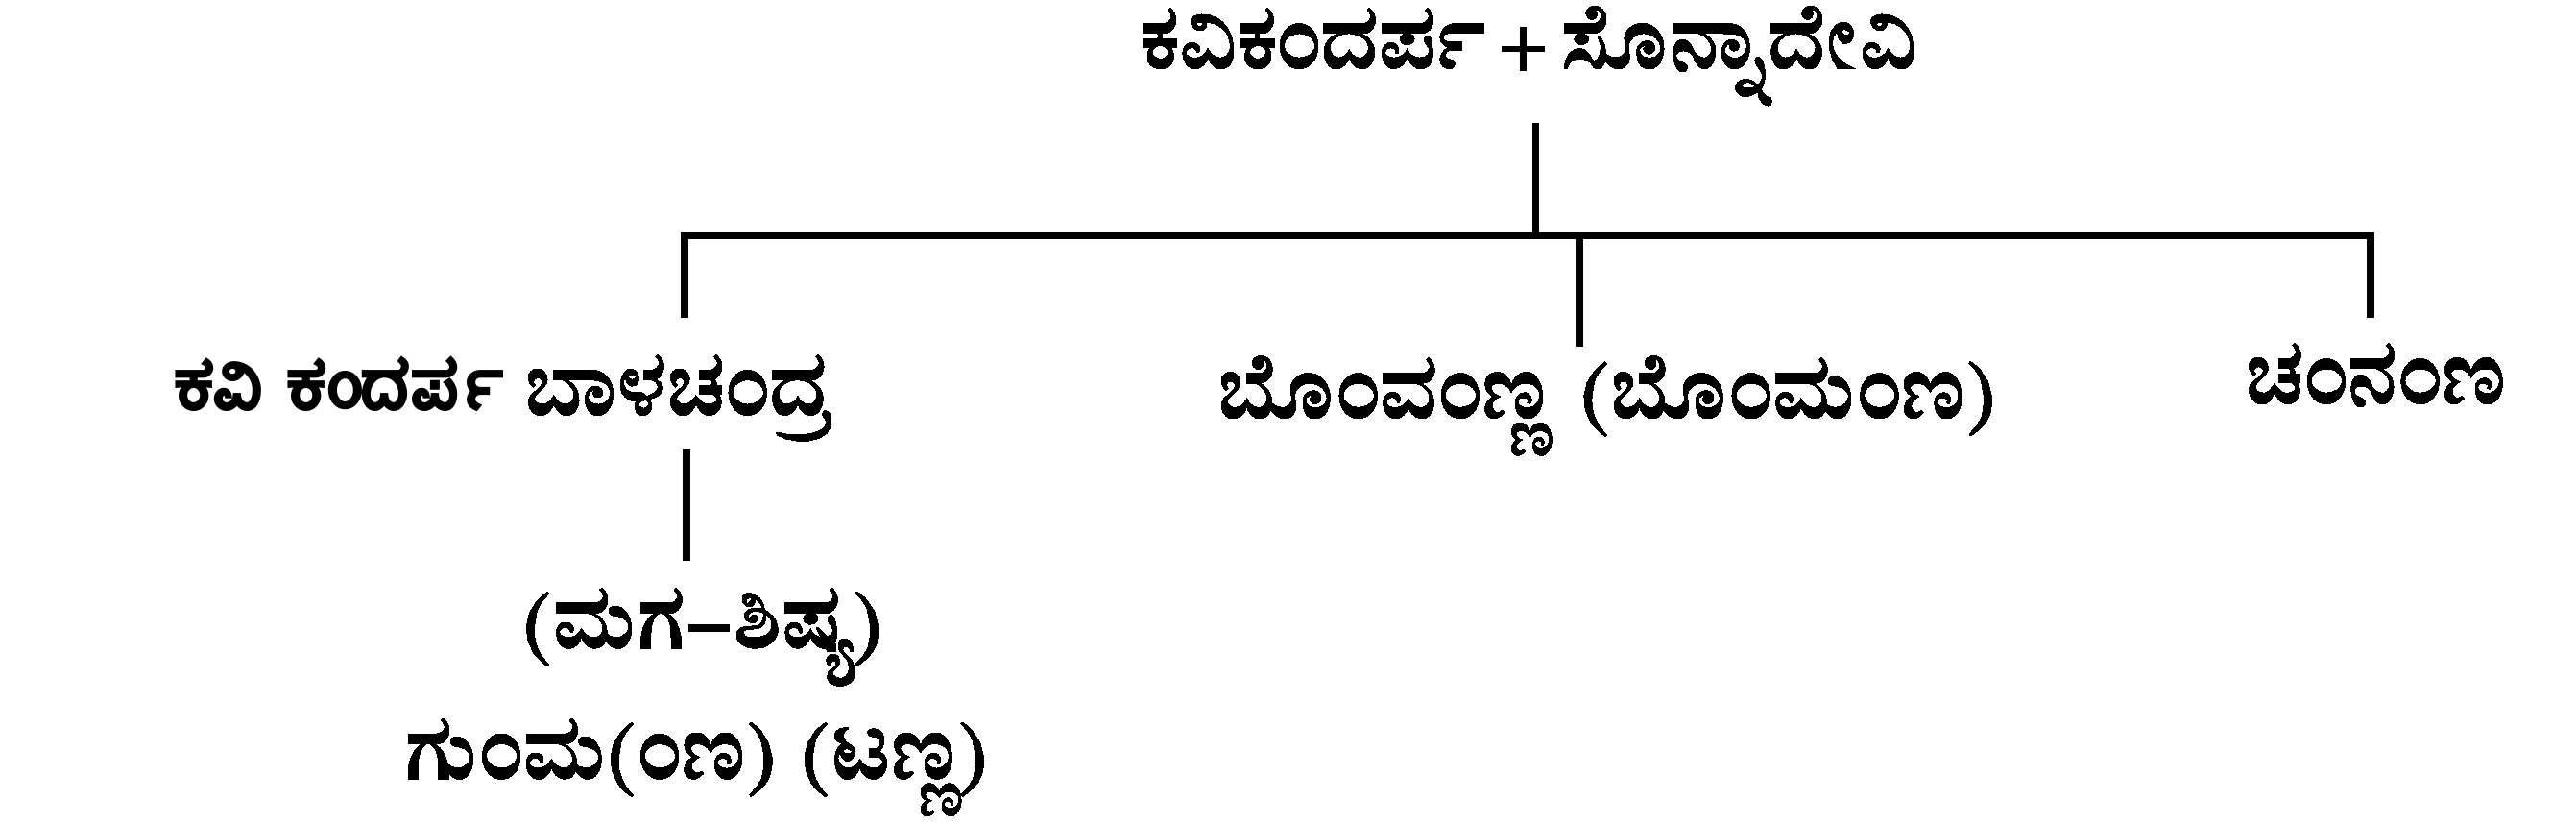
\includegraphics{images/chap4/chap4fig1.jpeg}
\end{figure}


ಕವಿಚರಿತೆಕಾರರು ಇವನನ್ನು ಬಾಳಚಂದ್ರ ಕವಿಕಂದರ್ಪ\index{ಬಾಳಚಂದ್ರ ಕವಿಕಂದರ್ಪ} ಎಂದು ಗುರುತಿಸಿದ್ದಾರೆ. “ಈತನು ಜನ್ನಕವಿಯ ಪತ್ನಿಯಾದ ಲಕುಮಾದೇವಿಯ ಗುರುವೆಂದು ಅನಂಥನಾಥಪುರಾಣದಿಂದ ತಿಳಿದುಬರುತ್ತದೆ. ಈತನ ಸಕಲಚಂದ್ರನ ಮಗನಾದ ಮಾಧವಚಂದ್ರನ ಶಿಷ್ಯ. ಪಾರ್ಶ್ವಪಂಡಿತನೂ ಕೂಡಾ ಸ್ತುತಿಸಿರುವ ಬಾಳಚಂದ್ರನೂ ಇವನೇ ಆಗಿರಬಹುದು. ಇವನು ವಕ್ರೋಕ್ತಿಯಲ್ಲಿ ಪ್ರಗಲ್ಬನೆಂದು ತಿಳಿಯುತ್ತದೆ. ಬೆಳಗಾವಿಯ\index{ಬೆಳಗಾವಿ} ಎರಡು ಶಿಲಾಶಾಸನಗಳನ್ನು ಬಾಳಚಂದ್ರಕಂದರ್ಪನು ಬರೆದಿದ್ದು, ಇವನು ಮಾಧವಚಂದ್ರ ತ್ರೈವಿದ್ಯನ ಶಿಷ್ಯನೆಂಬುದು ಇದರಿಂದ ತಿಳಿದುಬರುತ್ತದೆ. ಈತನು ಸೌಂದತ್ತಿಯ ರಟ್ಟರ\index{ಸೌಂದತ್ತಿಯ ರಟ್ಟ} ನಾಲ್ಕನೇ ಕಾರ್ತಿವೀರ್ಯ\index{ಕಾರ್ತಿವೀರ್ಯ} ಹಾಗೂ ಅವನ ಶ‍್ರೀಕರಣ ಬೀಚಿರಾಜ\index{ಶ‍್ರೀಕರಣ ಬೀಚಿರಾಜ} ಇವರುಗಳಿಗೆ ಗುರುವಾಗಿ ಇವರ ಆಶ್ರಯದಲ್ಲಿ ಇದ್ದನೆಂದು ಹೇಳಬಹುದು. ಇವನ ರಚಿಸಿರುವ ಶಾಸನಗಳು ಬ್ರಿಟಿಷ್​ ಮ್ಯೂಸಿಯಂನಲ್ಲಿವೆ ಎಂದು ತಿಳಿದುಬರುತ್ತದೆ” ಎಂದು ಹೇಳಿ ಇವನ ಶಾಸನದಿಂದ ಕೆಲವು ಪದ್ಯಗಳನ್ನು ಕವಿಚರಿತೆಕಾರರು ಎತ್ತಿಕೊಟ್ಟಿದ್ದಾರೆ.\endnote{ ನರಸಿಂಹಾಚಾರ್ಯ, ಆರ್​., ಕರ್ನಾಟಕ ಕವಿಚರಿತೆ, ಪ್ರಥಮ ಸಂಪುಟ, ಪುಟ 367-68}

“ಕವಿ ಬಾಳಚಂದ್ರನು ತನ್ನ ಆಶ್ರಯದಾತನಾದ ರಟ್ಟರ ನಾಲ್ಕನೇ ಕಾರ್ತಿವೀರ್ಯನನ್ನು ವರ್ಣಿಸಿದ್ದಾನೆ. ಇದರಿಂದ ಕಾರ್ತಿವೀರ್ಯನು ಇವನ ಆಶ್ರಯದಾತನಾಗಿದ್ದನೆಂಬುದು ಸ್ಪಷ್ಟ. ಕವಿ ಬಾಳಚಂದ್ರನು ರಚಿಸಿದ ಎರಡು ಶಾಸನಗಳ ಕಾಲ ಕ್ರಿ.ಶ.1204. ಕವಿಕಂದರ್ಪ ಬಾಳಚಂದ್ರನೂ ವೇಣುಗ್ರಾಮದಲ್ಲಿದ್ದನೆಂದು ಹೇಳಬಹುದು. ಇವನು ಚತುರ್ಭಾಷಾ ಪಂಡಿತನಾಗಿದ್ದನು. ಇವನು ತನ್ನ ತಂದೆ ತಾಯಿಯರ ಬಗ್ಗೆ ಎಲ್ಲೂ ಹೇಳಿಕೊಂಡಿಲ್ಲ. ಮಾಧವಚಂದ್ರ ತ್ರೈವಿದ್ಯದೇವನು\index{ಮಾಧವಚಂದ್ರ ತ್ರೈವಿದ್ಯದೇವ} ಇವನ ಗುರು ಎಂದು ಶಾಸನಗಳಿಂದ ಸ್ಪಷ್ಟವಾಗುತ್ತದೆ. ಇವನನ್ನು ಪಾರ್ಶ್ವಪಂಡಿತ ಮುಂತಾದ ಕವಿಗಳು ಸ್ತುತಿಸಿದ್ದಾರೆ. ಕವಿಕಂದರ್ಪ ಬಾಳಚಂದ್ರನು ಜನ್ನ ಕವಿಯ ಹೆಂಡತಿಯಾದ ಲಕುಮಾದೇವಿಯ ಗುರುವಾಗಿದ್ದನು ಎಂದು ಡಾ. ಬಿ.ಆರ್​. ಹಂದೂರ್​ ಅವರು ಹೇಳಿದ್ದಾರೆ.\endnote{ ಹಂದೂರ, ಡಾ॥ ಬಿ.ಆರ್​., ಜೈನಪರಂಪರೆಗೆ ಬೆಳಗಾವಿ ಪ್ರಾದೇಶಿಕ ಕೊಡುಗೆ, ಪುಟ 313-315} ತಿಪ್ಪೂರು ಶಾಸನವು ಈತನ ತಂದೆ ತಾಯಿಗಳ ಹೆಸರನ್ನು ಮತ್ತು ಇವನ ತಮ್ಮಂದಿರ ಹೆಸರನ್ನು, ಮತ್ತು ಇವನ ಶಿಷ್ಯನ ಹೆಸರನ್ನೂ ಹೇಳಿರುವುದರಿಂದ ಬಹಳ ಪ್ರಮುಖವಾದ ಶಾಸನವಾಗಿದೆ.

\textbf{ವಾಸುಪೂಜ್ಯರ\index{ವಾಸುಪೂಜ್ಯ} ಶಿಷ್ಯ ಸಕಳಚಂದ್ರ\index{ಸಕಳಚಂದ್ರ}:} ಮೂಲಸಂಘದ ಕಾಣೂರ್ಗಣದ ತಿಂತ್ರಿಣೀಕ ಗಚ್ಛದ ಕೊಂಡಕುಂದನ್ವಯದ ವಾಸುಪೂಜ್ಯದೇವರ ಶಿಷ್ಯರು ಸಕಳಚಂದ್ರದೇವರು ರಾಜಪೂಜ್ಯರಾಗಿದ್ದರೆಂದು ಕೂರಿಗಿಹಳ್ಳಿಯ\index{ಕೂರಿಗಿಹಳ್ಳಿ} ಗವುಡರು ಬಸ್ತಿಯಲ್ಲಿ ಕಟ್ಟಿಸಿದ ಪಾರ್ಶ್ವನಾಥ ಬಸದಿಯ\index{ಪಾರ್ಶ್ವನಾಥ ಬಸದಿ} ಶಾಸನದಲ್ಲಿ ಸ್ತುತಿತಸಲಾಗಿದೆ.\endnote{ ಎಕ 6 ಶ‍್ರೀಪ 74 ಬಸ್ತೀಪುರ 1422} ಕೂರ್ಗಳ್ಳಿಗೆ ಸಮೀಪ ಇರುವ ಬಸ್ತಿಪುರ\index{ಬಸ್ತಿಪುರ} ಗ್ರಾಮದ ಬಳಿ ಬಂಡೆಯ ಮೇಲೆ ಈ ಶಾಸನವಿದೆ. ಆದರೆ ಈಗ ಅಲ್ಲಿ ಬಸದಿ. ಇದ್ದ ಯಾವುದೇ ಕುರುಹುಗಳಿಲ್ಲ.


\section*{ಜೈನತೀರ್ಥಗಳು\index{ಜೈನತೀರ್ಥಗಳು}}

ಮಂಡ್ಯ ಜಿಲ್ಲೆಯು ಜೈನ ಧರ್ಮದ ನೆಲೆಬೀಡಾಗಿತ್ತು. ಶ್ರವಣಬೆಳಗೊಳವು ಮಂಡ್ಯ ಜಿಲ್ಲೆಯ ಗಡಿಗೇ ಹೊಂದಿಕೊಂಡಿದೆ. ಜಿಲ್ಲೆಯಲ್ಲಿ ಅನೇಕ ಶಾಸನೋಕ್ತ ಜೈನ ಕೇಂದ್ರಗಳ ಜೊತೆಗೆ ಕೆಲವು ಪ್ರಮುಖ ಜೈನತೀರ್ಥಗಳು ಕೂಡಾ ಕಂಡುಬರುತ್ತವೆ.

\textbf{ಕನಕಗಿರಿ ತೀರ್ಥ\index{ಕನಕಗಿರಿ ತೀರ್ಥ}:} ಸಗರವಂಶದ ಮಣಲೆಯಾರನು ಕ್ರಿ.ಶ. 916 ರಲ್ಲಿ ಕನಕಗಿರಿಯ ತೀರ್ಥದ ಮೇಲೆ ಬಸದಿಯನ್ನು ಮಾಡಿಸಿ ಅರಸರ ಅಧ್ಯಕ್ಷತೆಯಲ್ಲಿ (ನೀತಿಮಾರ್ಗನ ಸಮ್ಮುಖದಲ್ಲಿ) ಕನಕಸೇನ ಭಟಾರರಿಗೆ\index{ಕನಕಸೇನ ಭಟಾರು} ದತ್ತಿಯಾಗಿ ಬಿಡುತ್ತಾನೆ.\endnote{ ಎಕ 7 ಮದ್ದೂರು 100 ಕೂಲಿಗೆರೆ 916} ಕನಕಗಿರಿ ತೀರ್ಥವು ಚಾಮರಾಜನಗರ ತಾಲ್ಲೂಕಿನ ಮಲಿಯೂರಾಗಿರಬಹುದು\index{ಮಲಿಯೂರು} ಎಂದು ಎಪಿಗ್ರಾಫಿಯಾ ಕರ್ನಾಟಿಕಾ ಸಂಪಾದಕರು ಹೇಳಿದ್ದಾರೆ.\endnote{ ಎಪಿಗ್ರಾಫಿಯಾ ಕರ್ನಾಟಿಕಾ, ಸಂಪುಟ 7, ಪೀಠಿಕೆ, ಪುಟ \engfoot{xlvii}} ಆದರೆ ಚಾಮರಾಜನಗರ ತಾಲ್ಲೂಕಿನ ಮಲೆಯೂರಿಗೆ ಕನಕಗಿರಿ ಎಂಬ ಹೆಸರು ಕ್ರಿ.ಶ.1355ರ ಶಾಸನದಲ್ಲಿ ಕಂಡುಬರುತ್ತದೆ.\endnote{ ಅದೇ} ಕನಕಗಿರಿ ತೀರ್ಥದ ಮೇಲೆ, ಎಂದರೆ ತಿಪ್ಪೂರಿನ\index{ತಿಪ್ಪೂರು} ಸಮೀಪದ ಬೆಟ್ಟದಮೇಲೆ ಮಣಲೆಯರನು ಬಸದಿಯನ್ನು ನಿರ್ಮಿಸಿ ಅದಕ್ಕೆ ತಿಪ್ಪೂರಿನ ಸುಂಕಗಳನ್ನೇ ದತ್ತಿಯಾಗಿ ಬಿಟ್ಟಿದ್ದಾನೆ. ಕನಕಗಿರಿ ತೀರ್ಥವು ತಿಪ್ಪೂರು ತೀರ್ಥದಲ್ಲಿ ಅಂತರ್ಗತವಾಗಿತ್ತೆಂದು ಹಂಪನಾ ಅವರು ಹೇಳಿರುವುದು ಸೂಕ್ತವಾಗಿದೆ.\endnote{ ನಾಗರಾಜಯ್ಯ, ಹಂ.ಪ. ಶಾಸನಗಳಲ್ಲಿ ಜೈನತೀರ್ಥಗಳು, ಪುಟ 16-17} ಇದೇ ತಿಪ್ಪೂರಿನ ಗುಡ್ಡದ ಮೇಲಿನ ಜಿನಬಿಂಬದ ಪೀಠದಲ್ಲಿ ಕಾಣೂರ್ಗಣದ ಭಾಳಚಂದ್ರದೇವನ\index{ಕಾಣೂರ್ಗಣದ ಭಾಳಚಂದ್ರದೇವ} ಉಲ್ಲೇಖವಿದೆ.\endnote{ ಎಕ 7 ಮ 53 ತಿಪ್ಪೂರು 12ನೇ ಶ.} ಬಹುಶಃ ಈತನು ಗಂಗರಾಜ ದಂಡ ನಾಯಕನಿಂದ ಕ್ರಿ.ಶ. 1117ರಲ್ಲಿ ತಿಪ್ಪೂರು ತೀರ್ಥಕ್ಕೆ ದಾನ ಸ್ವೀಕರಿಸಿದ ಇದೇ ಕಾಣೂರ್ಗಣದ ಮೇಘಚಂದ್ರ ಸಿದ್ಧಾಂತನ ಶಿಷ್ಯನಾಗಿರಬಹುದು. ಇಲ್ಲೇ ಇರುವ ವೀರಬಲ್ಲಾಳನ ಕಾಲದ ಇನ್ನೊಂದು ಶಾಸನದಲ್ಲಿ ತಿಪ್ಪೂರ ಕವಿಕಂದರ್ಪರ ಶಿಷ್ಯ\index{ಕವಿಕಂದರ್ಪರ ಶಿಷ್ಯ} ಬಾಲಚಂದ್ರದೇವರ\index{ಬಾಲಚಂದ್ರದೇವರು} ಉಲ್ಲೇಖವಿದೆ.\endnote{ ಎಕ 7 ಮ 52 ತಿಪ್ಪೂರು 12ನೇ ಶ.} ಆದುದರಿಂದ ಈ ತಿಪ್ಪೂರು\index{ತಿಪ್ಪೂರು} ಬಹಳ ಪ್ರಸಿದ್ಧವಾದ ಜೈನಕೇಂದ್ರವಾಗಿದ್ದು ಕನಕಗಿರಿ ತೀರ್ಥ ಎಂದು ಹೆಸರುವಾಸಿಯಾಗಿದ್ದಿರಬಹುದು.

\textbf{ತಿಪ್ಪೂರು ತೀರ್ಥ\index{ತಿಪ್ಪೂರು ತೀರ್ಥ}:} ಈಗ ಇದನ್ನು ಅರೆತಿಪ್ಪೂರು\index{ಅರೆತಿಪ್ಪೂರು} ಎಂದು ಕರೆಯಲಾಗುತ್ತದೆ. ಈ ಊರಿಗೆ ಸೇರಿದಂತೆ, ಶ್ರವಣಬೆಳಗೊಳದ ಮಾದರಿಯಲ್ಲಿ ಚಿಕ್ಕಬೆಟ್ಟ (ಜಿನಗುಡ್ಡ)\index{ಚಿಕ್ಕಬೆಟ್ಟ (ಜಿನಗುಡ್ಡ)}, ದೊಡ್ಡಬೆಟ್ಟ (ಸವಣಪ್ಪನ ಬೆಟ್ಟ)\index{ದೊಡ್ಡಬೆಟ್ಟ (ಸವಣಪ್ಪನ ಬೆಟ್ಟ)} ಎಂಬ ಎರಡು ಬೆಟ್ಟಗಳಿದು, ಜಿನಗುಡ್ಡದ ಮೇಲೆ ಬಸದಿಯೂ, ಗಂಗರಾಜನ ಶಾಸನವೂ, ಜಿನಬಿಂಬಗಳೂ, ನೀರಿನ ಡೊಣೆಯೂ ಇವೆ. ದೊಡ್ಡ ಬೆಟ್ಟದ ಮೇಲೆ, ಗಂಗರಾಜನಿಂದ ಸ್ಥಾಪಿತವಾಗಿರಬಹುದಾದ ಗೊಮ್ಮಟೇಶ್ವರ ಮೂರ್ತಿ ಇದೆ. ಗಂಗರಾಜನು ತಿಪ್ಪೂರನ್ನು ಕೊಡುಗೆಯಾಗಿ ಪಡೆದು ಅದನ್ನು ತನ್ನ ಗುರು, ಕಾಣೂರ್ಗಣದ, ತಿಂತ್ರಿಣೀಕ ಗಚ್ಛದ ಮೇಘಚಂದ್ರ ಸಿದ್ಧಾಂತ ದೇವರಿಗೆ ದತ್ತಿಯಾಗಿ ಬಿಡುತ್ತಾನೆ.\endnote{ ಎಕ 7 ಮ 54 ತಿಪ್ಪೂರು 1117} ಬಹುಶಃ ಮಣಲೆಯರನು ಬಿಟ್ಟಿದ್ದ ದತ್ತಿಯು ತಪ್ಪಿಹೋಗಿ, ತಿಪ್ಪೂರು ತೀರ್ಥವು ಹಾಳಾಗಿರಲು, ಗಂಗರಾಜನು ಪುನಃ ರಾಜನಿಂದ ಆ ಊರನ್ನೇ ದತ್ತಿಯಾಗಿ ಪಡೆದು, ತಿಪ್ಪೂರನ್ನು ತೀರ್ಥವನ್ನು ಪುನರುಜ್ಜೀವಿಸಿರುವಂತೆ ಕಂಡು ಬರುತ್ತದೆ. ತಿಪ್ಪೂರಿಗೆ ಸಮೀಪದ ಹಾದರವಾಗಿಲು (ಹಾಗಲಹಳ್ಳಿ) ಗ್ರಾಮವನ್ನು, ಸುಮಾರು ಇದೇ ಕಾಲದ ಶಾಸನದಲ್ಲಿ ತಿಪ್ಪೂರು ತೀರ್ಥದ ಹಾದರವಾಗಿಲು ಎಂದು ಕರೆದಿದೆ.\endnote{ ಎಕ 7 ಮ 103 ಹಾದರವಾಗಿಲು 12ನೇಶ.} ಪುನ: ಕ್ರಿ.ಶ.1619ರ ಶಾಸನದಲ್ಲೂ ತಿಪ್ಪೂರು ತೀರ್ಥದ ಹಾದರವಾಗಿಲ ಉಲ್ಲೇಖವಿದೆ.\endnote{ ಎಕ 7 ಮ 106 ಹಾದರವಾಗಿಲು 1619} ಈ ಶಾಸನದಲ್ಲಿ \textbf{ಶ‍್ರೀ ಮೂಲಸಂಘದ ಕಾನೂರ್ಗ್ಗಣದ ತಿಂತ್ರಿಣಿಕಗಚ್ಛದ ಮೇಘಚಂದ್ರ ಸಿದ್ಧಾಂತ ದೇವರ ಶಿಷ್ಯರು ಕುಮುದಚಂದ್ರ ಪಂಡಿತದೇವರು\index{ಕುಮುದಚಂದ್ರ ಪಂಡಿತದೇವರು}, ಅವರ ಸಾಧರ್ಮಿಗಳು ಶ್ರುತಕೀರ್ತಿ ಪಂಡಿತ ದೇವರು\index{ಶ್ರುತಕೀರ್ತಿ ಪಂಡಿತ ದೇವರು}, ಆದಿನಾಥ ಪಂಡಿತ ದೇವರ ಉಲ್ಲೇಖವಿದ್ದು,} ಗಂಗರಾಜನ ಕಾಲದ ಜಿನಮುನಿ ಪರಂಪರೆ ಮುಂದುವರಿದಿರುವುದನ್ನು ಸೂಚಿಸುತ್ತದೆ. ಹಾದರವಾಗಿಲು ತಿಪ್ಪೂರು ತೀರ್ಥದ ದತ್ತಿ ಗ್ರಾಮವಾಗಿತ್ತೆಂದು ಹೇಳಬಹುದು.

\textbf{ಬಿಂಡಿಗನವಿಲೆ ತೀರ್ಥ\index{ಬಿಂಡಿಗನವಿಲೆ ತೀರ್ಥ}/ಕಂಬದಹಳ್ಳಿ ತೀರ್ಥ\index{ಕಂಬದಹಳ್ಳಿ ತೀರ್ಥ}:} ಬಿಂಡಿಗನವಿಲೆ ಮತ್ತು ಕಂಬದಹಳ್ಳಿ ಈ ಎರಡೂ ತೀರ್ಥಗಳನ್ನೂ ಹಂಪನಾ ಅವರು ಬೇರೆ ಬೇರೆಯಾಗಿಯೇ ಗುರುತಿಸಿದ್ದಾರೆ.\endnote{ ನಾಗರಾಜಯ್ಯ, ಡಾ॥ ಹಂಪ., ಶಾಸನಗಳಲ್ಲಿ ಜೈನತಿರ್ಥಗಳು, ಪುಟ 14-15 ಮತ್ತು ಪುಟ 47} ಕಂಬದಹಳ್ಳಿಯ ಮಾನಸ್ಥಂಭದ ಮೇಲೆ ಗಂಗರ ಕಾಲದ ಜೈನಯತಿಗಳ ಪರಂಪರೆ, ಸ್ತುತಿ ಇದ್ದರೂ ತೀರ್ಥವೆಂಬ ಉಲ್ಲೇಖವಿಲ್ಲ ಈ ಶಾಸನದ ಕೆಳಗಿರುವ ಕ್ರಿ.ಶ.1118ರ ಗಂಗರಾಜನ ಶಾಸನದಲ್ಲಿ ಮೊದಲ ಬಾರಿಗೆ ಬಿಂಡಿಗನವಿಲೆ ತೀರ್ಥದ ಹೆಸರು ಬರುತ್ತದೆ.\endnote{ ಎಕ 7 ನಾಮಂ 33 ಬಿಂಡಿಗನವಿಲೆ 9ನೇ ಶ. ಮತ್ತು 1118}ದಂಡನಾಯಕ ಪಾರ್ಶ್ವದೇವನ ಕ್ರಿ.ಶ. 1168ರ ಕಂಬದಹಳ್ಳಿ ಶಾಸನದಲ್ಲಿ “ದೇವಕ್ಷೇತ್ರ ಬಿಂಡಿಗನವಿಲೆ” ಎಂಬ ಉಲ್ಲೇಖವಿದ್ದು, ದೇವಕ್ಷೇತ್ರವೆಂದರೆ ತೀರ್ಥವೆಂದು ತಿಳಿಯ\-ಬಹುದು.\endnote{ ಎಕ 7 ನಾಮಂ 26 ಬಿಂಡಿಗನವಿಲೆ 1168} ಇದರಿಂದ ಬಿಂಡಿಗನವಿಲೆಯೂ, ಕಂಬದಳ್ಳಿಯೂ ಒಂದೇ ಎಂದು ತಿಳಿಯಬಹುದು. ಕಂಬದಹಳ್ಳಿ ಎಂಬ ಹೆಸರು ಕ್ರಿ.ಶ.1145ರ ಒಂದನೇ ನರಸಿಂಹನ ಶಾಸದಲ್ಲಿ ಮೊದಲಬಾರಿಗೆ ಬರುತ್ತದೆ. ಆದರೆ ಇದರಲ್ಲಿ ತೀರ್ಥದ ಪ್ರಸ್ತಾಪವಿಲ್ಲ.\endnote{ ಎಕ 7 ನಾಮಂ 30 ಕಂಬದಹಳ್ಳಿ 1145} ದಂಡನಾಯಕ ಪಾರ್ಶ್ವದೇವನ ಶಾಸನದ ಆಧಾರದ ಮೇಲೆ ಕಂಬದಹಳ್ಳಿಯು ಹನಸೋಗೆ ಮಠಕ್ಕೆ\index{ಹನಸೋಗೆ ಮಠ} ಪ್ರತಿಬದ್ಧವಾಗಿತ್ತೆಂದು ಹಂಪನಾ ಅಭಿಪ್ರಾಯಪಟ್ಟಿದ್ದಾರೆ.\endnote{ ನಾಗರಾಜಯ್ಯ, ಡಾ॥ ಹಂ.ಪ., ಶಾಸನಗಳಲ್ಲಿ ಜೈನತೀರ್ಥಗಳು, ಪುಟ 14} ಎರಡನೆಯ ಬಲ್ಲಾಳನ ಕಾಲದ ಶಾಸನದಲ್ಲಿ ಎಕ್ಕೋಟಿ ಮಹಾರುದ್ರರು\index{ಎಕ್ಕೋಟಿ ಮಹಾರುದ್ರರು} ಸೇರಿ “ಕಂಬದಹಳ್ಳಿ ತೀರ್ಥ” ವನ್ನು ಎಕ್ಕೋಟಿ ಜಿನಾಲಯವೆಂದು ಘೋಷಿಸಿದರು.\endnote{ ಎಕ 7 ನಾಮಂ 31 ಕಂಬದಹಳ್ಳಿ 12-13ನೇ ಶ.} ಇದರಿಂದ ಕಂಬದಹಳ್ಳಿ ಮತ್ತು ಬಿಂಡಿಗನವಿಲೆ ತೀರ್ಥಗಳು ಬೇರೆ ಬೇರೆ ಎಂದು ಅಭಿಪ್ರಾಯಕ್ಕೆ ಬರಲಾಗಿದೆ. ಈ ಕಾಲಕ್ಕೆ ಬಿಂಡಿಗನವಿಲೆ ಮತ್ತು ಕಂಬದಹಳ್ಳಿಗಳು ಬೇರೆಬೇರೆಯಾಗಿ ಗುರುತಿಸಿಕೊಂಡಿದ್ದು, ಬಸದಿಗಳಿದ್ದ ಕಂಬದಹಳ್ಳಿಯನ್ನು ಮಾತ್ರ ತೀರ್ಥವೆಂದು ಕರೆಯಲಾಗುತ್ತಿತ್ತೆಂದು ಹೇಳಬಹುದು. ಬಿಂಡಿಗನವಿಲೆಯು ಶೈವ ಧರ್ಮದ ಕೇಂದ್ರವಾಗಿ ನಂತರದಲ್ಲಿ ವೈಷ್ಣವ ಕ್ಷೇತ್ರವಾಯಿತೆಂದು ಹೇಳಬಹುದು.

\textbf{ತ್ರಿಭುವನ ತಿಳಕದ ತೀರ್ಥ\index{ತ್ರಿಭುವನ ತಿಳಕದ ತೀರ್ಥ}:} ವಿಷ್ಣುವರ್ಧನನ ಪಿರಿಯರಸಿ ಚಂದಲದೇವಿಯು ತನಗೆ ಬಳುವಳಿಯಾಗಿ ಬಂದ ಮಂದಗೆರೆ ಶ್ರುತಿಯ ಕಾವನಹಳ್ಳಿ ಗ್ರಾಮವನ್ನು ತ್ರಿಭುವನ ತಿಳಕ ತೀರ್ಥದಲ್ಲಿದ್ದ ವೀರ ಕೊಂಗಾಳ್ವ ಜಿನಾಲಯದ\index{ವೀರ ಕೊಂಗಾಳ್ವ ಜಿನಾಲಯ} ಋಷಿಗಳ ಆಹಾರದಾನಕ್ಕೆ\index{ಆಹಾರದಾನ} ದತ್ತಿ ಬಿಡುತ್ತಾಳೆ.\endnote{ ಎಕ 6 ಕೃಪೇ 21 ಶ್ರವಣನಹಳ್ಳಿ 1116-17} ಇಂದಿನ ಮಹಾರಾಷ್ಟ್ರ ರಾಜ್ಯದ ಕೊಲ್ಲಾಪುರವು\index{ಕೊಲ್ಲಾಪುರ} ತ್ರಿಭುವನ ತಿಳಕ ತೀರ್ಥವೆಂದು ತಿಳಿದುಬರುತ್ತದೆ. ಆದರೆ ಅಷ್ಟುದೂರದ ಕೊಲ್ಲಾಪುರ\-ದಲ್ಲಿದ್ದ ಜಿನಾಲಯಕ್ಕೆ, ಈ ಊರನ್ನು ದತ್ತಿಯಾಗಿ ಬಿಡುವುದು ಸಂಭವನೀಯವಲ್ಲ. ಕೊಂಗಾಳ್ವರು ಇಲ್ಲಿಂದ ಕೊಲ್ಲಾಪುರಕ್ಕೆ ಹೋಗಿ ಅಲ್ಲಿ ವೀರಕೊಂಗಾಳ್ವ ಜಿನಾಲಯವನ್ನು ನಿರ್ಮಿಸುವುದು ಸಂಭವನೀಯವಲ್ಲ. ಅದೂ ಅಲ್ಲದೆ ಕೊಲ್ಲಾಪುರದಲ್ಲಿರುವುದು ಚಂದ್ರಪ್ರಭ ತೀರ್ಥಂಕರ ಜಿನಾಲಯವಾಗಿದೆ.\endnote{ ನಾಗರಾಜಯ್ಯ, ಹಂ.ಪ., ಶಾಸನಗಳಲ್ಲಿ ಜೈನತೀರ್ಥಗಳು, ಪುಟ. 26} ಗ್ರಾಮವನ್ನು ದತ್ತಿ ಬಿಟ್ಟಿರುವುದು ವೀರಕೊಂಗಾಳ್ವ ಜಿನಾಲಯಕ್ಕೆ ಆದುದರಿಂದ ಈ ತ್ರಿಭುವನ ತಿಳಕ ತೀರ್ಥವು ಇಂದು ಶಾಸನ ಇರುವ ಶ್ರವಣನಹಳ್ಳಿ (ಕಾವನಹಳ್ಳಿ)\index{ಶ್ರವಣನಹಳ್ಳಿ (ಕಾವನಹಳ್ಳಿ)} ಆಗಿರಬಹುದು. ಒಂದೇ ಹೆಸರಿನ ಎರಡು ತೀರ್ಥಗಳು ಇದ್ದಿರುವ ಸಾಧ್ಯತೆ ಇದೆ. ತ್ರಿಭುವನ ತಿಲಕವೆಂಬ ಬಸದಿಯನ್ನು ಪಂಪನ ತಮ್ಮ ಜಿನವಲ್ಲಭನು ನಿರ್ಮಿಸಿದನೆಂದು ಕುರ್ಕ್ಯಾಲ್​ ಶಾಸನದಿಂದ ತಿಳಿದುಬರುತ್ತದೆ.\endnote{ ಅಣ್ಣಿಗೇರಿ,ಎ.ಎಂ., ಶೇಷಶಾಸ್ತ್ರಿ ಆರ್​., ಜಿನವಲ್ಲಭನ ಶಾಸನ, ಶಾಸನ ಸಂಗ್ರಹ, ಪುಟ 12}

\textbf{ಕೆಲ್ಲಂಗೆರೆಯ ತೀರ್ಥ\index{ಕೆಲ್ಲಂಗೆರೆಯ ತೀರ್ಥ}:} ಇಂದಿನ ನಾಗಮಂಗಲ ತಾಲ್ಲೂಕು, ಕೆಲಗೆರೆಯೇ ಪ್ರಾಚೀನ ಕೆಲ್ಲಂಗೆರೆ ತೀರ್ಥವೆಂದು ಹೇಳಬಹುದು. ಕೆಲ್ಲಂಗೆರೆ ತೀರ್ಥದ ಹೆಸರು ಮೊದಲಬಾರಿಗೆ, ಹೊಯ್ಸಳರ ಒಂದನೆಯ ನರಸಿಂಹನ ಮಹಾಪ್ರಧಾನ ಹುಳ್ಳ ಚಮೂಪನ ಕ್ರಿ.ಶ.\enginline{1159}ರ ಶ್ರವಣಬೆಳಗೊಳದ ಭಂಡಾರ ಬಸದಿಯ ಶಾಸನದಲ್ಲಿ ಉಲ್ಲೇಖಿತವಾಗಿದೆ. ಕೆಲ್ಲಂಗೆರೆಯು ಗಂಗರಿಂದ ನಿರ್ಮಿತವಾದ ಪ್ರಖ್ಯಾತ ಆದಿತೀರ್ಥವಾಗಿದ್ದು, ಕಾಲವಶದಿಂದ ನಾಮಾವಶೇಷವಾಗಿತ್ತೆಂದು, ಹುಳ್ಳಚಮೂಪನು\index{ಹುಳ್ಳಚಮೂಪ} ಅದನ್ನು ಜೀರ್ಣೋದ್ಧಾರ ಮಾಡಿ ಪಂಚ ಬಸದಿಗಳನ್ನು\index{ಪಂಚ ಬಸದಿ} ನಿರ್ಮಿಸಿದನೆಂದು, ಈ ಶಾಸನದಿಂದ ತಿಳಿದುಬರುತ್ತದೆ.\endnote{ ಎಕ 2 ಶ್ರಬೆ 476 ಶ್ರವಣಬೆಳಗೊಳ (ಭಂಡಾರ ಬಸದಿ) 1159} ಈ ವಿಚಾರವನ್ನು ಹೇಳುವ ಶಾಸನದ ಪದ್ಯಗಳು ಈ ಕೆಳಕಂಡಂತಿವೆ.

\begin{verse}
\textbf{ಆ ಕೆಲ್ಲಂಗೆರಱೆಯಾದಿ ತೀರ್ಥಮದು ಮುನ್ನಂ ಗಂಗರಿಂ ನಿರ್ಮ್ಮಿತಂ\\ ಲೋಕಪ್ರಸ್ತುತಮಾಯ್ತು ಕಾಲವಶದಿಂ ನಾಮಾವಶೇಷಂ ಬಳಿ\\ ಕ್ಕಾಕಲ್ಪ ಸ್ಥರಮಾಗೆ ಮಾಡಿಸಿದನೀ ಭಾಸ್ವಜ್ಜಿನಾಗಾರಮಂ\\ ಶ‍್ರೀಕಾನ್ತಂ ತಳದಿನ್ದಮೆಯ್ದೆ ಕಳಸಂ ಶ‍್ರೀ ಹುಳ್ಳದಂಡಾಧಿಪಂ}
\end{verse}

\begin{verse}
\textbf{ಪಂಚಮಹಾವಸತಿಗಳಂ\\ ಪಂಚಕಲ್ಯಾಣವಾಂಛೆಯಿಂ ಹುಳ್ಳ ಚಮೂ\\ ಪಂ ಚತುರಂ ಮಾಡಿಸಿದಂ \\ ಕಾಂಚನನಗ ಧೈರ್ಯ್ಯನೆಸೆವ ಕೆಲ್ಲಂಗೆಱೆಯೊಳ್​}
\end{verse}

ಮಹಾಪ್ರಧಾನ ಭಂಡಾರಿ ಹುಳ್ಳಚಮೂಪನ ಕ್ರಿ.ಶ. \enginline{1163}ರ ಶ್ರವಣಬೆಳಗೊಳ ಚಿಕ್ಕಬೆಟ್ಟದ ಮಹಾ ನವಮಿ ಮಂಟಪದಲ್ಲಿರುವ ಶಾಸನದಲ್ಲಿಯೂ, ಕೆಲ್ಲಂಗೆರೆಯ ತೀರ್ಥದ\index{ಕೆಲ್ಲಂಗೆರೆಯ ತೀರ್ಥ} ಪ್ರಸ್ತಾಪವಿದ್ದು, ಮಹಾಪ್ರಧಾನ ಹಿರಿಯ ಭಂಡಾರಿ ಹುಳ್ಳ ಚಮೂಪನು, ತನ್ನ ಗುರುಗಳಾದ ಶ‍್ರೀ ಕೊಂಡ ಕುಂದಾನ್ವಯದ, ಮೂಲ ಸಂಘದ, ದೇಶಿಯ ಗಣದ, ಪುಸ್ತಕ ಗಚ್ಛದ ದೇವಕೀರ್ತಿ ಪಂಡಿತರ ಪರೋಕ್ಷ ವಿನಯವಾಗಿ ಶ‍್ರೀ ಕೊಲ್ಲಾಪುರ ರೂಪನಾರಾಯಣ ಬಸದಿಯ ಪ್ರತಿಬದ್ಧ ಕೆಲ್ಲಂಗೆರೆಯ ಪ್ರತಾಪಪುರವನ್ನು ಪುನರುದ್ಧಾರ ಮಾಡಿದನೆಂದು ಹೇಳಿದೆ \endnote{ ಎಕ 2 ಶ್ರಬೆ 71 ಚಿಕ್ಕಬೆಟ್ಟ (ಮಹಾನವಮಿ ಮಂಟಪ) 1163} ಇದರಿಂದ ಕೆಲ್ಲಂಗೆರೆಯು ಕೊಲ್ಲಾಪುರದ ಬಸದಿಗೆ\index{ಕೊಲ್ಲಾಪುರದ ಬಸದಿ} ಸೇರಿದ್ದ ತೀರ್ಥವಾಗಿತ್ತೆಂಬುದು ತಿಳಿದುಬರುತ್ತದೆ.

ಹಾಸನ ಜಿಲ್ಲೆ, ಬೇಲೂರು ತಾಲ್ಲೂಕು, ಹಳೆಯಬೀಡಿನ ಬಸ್ತಿಹಳ್ಳಿಯ ಪರಿಸರವೇ ಕೆಲ್ಲಂಗೆರೆಯ ತೀರ್ಥ ಎಂದು, ಇದು ಯಾಪನೀಯ ಕೇಂದ್ರವೆಂದು, ಇದು ಕೊಲ್ಲಾಪುರದ ಬಸದಿಗೆ ಪ್ರತಿಬದ್ಧವಾಗಿತ್ತೆಂದು ಹಂ.ಪ.ನಾ. ಅವರು ಹೇಳಿದ್ದಾರೆ.\endnote{ ನಾಗರಾಜಯ್ಯ, ಡಾ॥ ಹಂ.ಪ., ಶಾಸನಗಳಲ್ಲಿ ಜೈನತೀರ್ಥಗಳು, ಪುಟ 23-24} ಕೆಳಗೆರೆಯಲ್ಲಿರುವ ಮೂರನೆಯ ನರಸಿಂಹನ ಶಾಸನದಲ್ಲಿ ಮೂಲಸಂಘದ, ಬಳಾತ್ಕರಗಣದ\index{ಬಳಾತ್ಕರಗಣ} ಜೈನಯತಿ ಪರಂಪರೆಯನ್ನು ನೀಡಿದೆ ಮತ್ತು ವೀರನಾರಸಿಂಹನು ದೋರಸಮುದ್ರದ ತ್ರಿಕೂಟ ರತ್ನತ್ರಯ ಶಾಂತಿನಾಥ ಬಸದಿಗೆ\index{ತ್ರಿಕೂಟ ರತ್ನತ್ರಯ ಶಾಂತಿನಾಥ ಬಸದಿ} ಚಿಕ್ಕಕಂನೆಯನಹಳ್ಳಿಯನ್ನು\index{ಚಿಕ್ಕಕಂನೆಯನಹಳ್ಳಿ} ಮಾಘನಂದಿ ಸಿದ್ಧಾಂತ ದೇವರಿಗೆ ದತ್ತಿನೀಡಿದನೆಂದು ಹೇಳಿದೆ.\endnote{ ಎಕ 7 ನಾಮಂ 60 ಕೆಲಗೆರೆ 13ನೇ ಶ.} ಕನ್ನೇನಹಳ್ಳಿಯು ಕೆಲಗೆರೆಯ ಪಕ್ಕದಲ್ಲೇ ಇದೆ. ಆದರೆ ಈ ಶಾಸನದಲ್ಲಿ ಕೆಲ್ಲಂಗೆರೆ ಎಂಬ ಹೆಸರಿಲ್ಲ. ಇಲ್ಲಿರುವ ಕ್ರಿ.ಶ.\enginline{15}ನೇ ಶತಮಾನದ ವಿಜಯನಗರ ಕಾಲದ ಶಾಸನದಲ್ಲಿ ಮಾತ್ರ ಈ ಊರನ್ನು ಶ‍್ರೀ ವರದರಾಜಪುರವಾದ ಭಟ್ಟಾರಕದೇವನ ಕೆಲ್ಲಂಗೆರೆ\index{ವರದರಾಜಪುರವಾದ ಭಟ್ಟಾರಕದೇವನ ಕೆಲ್ಲಂಗೆರೆ} ಎಂದು ಹೇಳಿದೆ.\endnote{ ಎಕ 7 ನಾಮಂ 58 ಕೆಲಗೆರೆ 15ನೇ ಶ.} ಜೈನಕೆಂದ್ರವಾದ ಶ್ರವಣಬೆಳಗೊಳ, ಕಂಬದಹಳ್ಳಿ, ತಿಪ್ಪೂರು, ಬೆಳ್ಳೂರಿಗೆ ಸಮೀಪದಲ್ಲಿರುವ ಈ ಕೆಲ್ಲಂಗೆರೆಯೇ ಕೆಲ್ಲಂಗೆರೆಯ ತೀರ್ಥವಾಗಿದೆ ಎಂದು ಖಚಿತವಾಗಿ ಹೇಳಬಹುದು. ಕೆಲಗೆರೆಯಲ್ಲಿದ್ದ ಬಸದಿಯು ನಾಶವಾಗಿ ಮಾನಸ್ಥಂಭ ಮಾತ್ರ ಉಳಿದಿದೆ.

ಹಳೇಬೀಡು ಬೆಣ್ಣೆಗುಡ್ಡದ ಬಳಿ ಇರುವ ಶಿಲಾಶಾಸನದಲ್ಲಿ “ಕಲುಕಣಿನಾಡ ಕೆಲ್ಲಂಗೆಱೆ(ಯ)\index{ಕಲುಕಣಿನಾಡ ಕೆಲ್ಲಂಗೆಱೆ(ಯ)} ತಂನ ಕಾಲುವಳ್ಳಿ\-ಗಳಪ್ಪ ಕರಡಿಯಹಳ್ಳಿ, ಹೋತನಡಕೆಯಹಳ್ಳಿ, ಅರೆಯಹಳ್ಳಿ, ಅಜ್ಜನಾಯಕನಹಳ್ಳಿ, ಹೂಲಿಯಕೆರೆ, ಚೊಟ್ಟನಹಳ್ಳಿ, ನರೆಗನಹಳ್ಳಿ, ಸೇರನಹಳ್ಳಿ, ಚೋಳೆಯನಹಳ್ಳಿ, ಲೊಕ್ಕಿಯಹಳ್ಳಿ, ಗೌರಿಯಹಳ್ಳಿ, ಕುಂಚದಹಳ್ಳಿ, ಹಿರಿಯಕಂನೆಯನಹಳ್ಳಿ, ಚಿಕ್ಕಕಂನೆಯನಹಳ್ಳಿಗಳನುಳ್ಳ ಆ ಕೆಲ್ಲಂಗೆಱೆಯ ಚತುಃಸ್ಸೀಮಾ” ಎಂದು ಹೇಳಿದ್ದು ಈ ಹಳ್ಳಿಗಳನ್ನು ಮೂರನೆಯ ನರಸಿಂಹನು, ಮೂಲಸಂಘದ, ಬಲಾತ್ಕರ ಗಣದ, ದೋರ ಸಮುದ್ರದ ತ್ರಿಕೂಟ ರತ್ನತ್ರಯ ಶಾಂತಿನಾಥ ಜಿನಾಲಯಕ್ಕೆ ದತ್ತಿಬಿಟ್ಟನೆಂದು ಹೇಳಿದೆ.\endnote{ ಎಕ 9 ಬೇ 321 ಹಳೇಬೀಡು 1265} ಈ ಹಳ್ಳಿಗಳೆಲ್ಲಾ ಇಂದಿಗೂ ಕೂಡಾ ನಾಗಮಂಗಲ ತಾಲ್ಲೂಕಿನ ಕೆಲ್ಲಂಗೆರೆಯ ಅಕ್ಕಪಕ್ಕದಲ್ಲೇ ಇವೆ. ಈ ಪ್ರದೇಶವು ಕಲುಕಣಿ ನಾಡಿಗೆ ಸೇರಿತ್ತೆಂಬುದು ಸ್ಪಷ್ಟ. ಸೇರನಹಳ್ಳಿಯೇ ಯಾಲಾದಹಳ್ಳಿ\index{ಯಾಲಾದಹಳ್ಳಿ} ಶಾಸನೋಕ್ತವಾದ, ದೇವರಾಜನು ಪಾರ್ಶ್ವಪುರವನ್ನಾಗಿ ಮಾಡಿ ಬಸದಿಯನ್ನು ನಿರ್ಮಿಸಿದ ಸೂರನಹಳ್ಳಿಯಾಗಿದೆ.\endnote{ ಎಕ 7 ನಾಮಂ 64 ಯಾಲಾದಹಳ್ಳಿ 1145} ಆದರೆ ಇಂದು ಈ ಊರು ಬಸದಿಯಿಂದ ದೂರದಲ್ಲಿದ್ದು, ಬಸದಿಯು ಮಾತ್ರ ಜೀರ್ಣಾವಸ್ಥೆಯಲ್ಲಿ\break ಉಳಿದುಕೊಂಡಿದೆ. ಇಲ್ಲಿದ್ದ ದೊಡ್ಡ ಶಾಸನವನ್ನು ಬೆಳ್ಳೂರು ಬಸದಿಗೆ ಸಾಗಿಸಲಾಗಿದೆ. ಶಾಸನೋಕ್ತ ಹಳ್ಳಿಗಳು, ಕರಡಹಳ್ಳಿ, \hbox{ಹುಂಡೇನಹಳ್ಳಿ}, ಅರೆಹಳ್ಳಿ, ಹುಲ್ಲೇಕೆರೆ, ಚೊಟ್ಟಕ್ಯಾತನಹಳ್ಳಿ, ನರಗಲು\index{ನರಗಲು}, ಸೂರನಹಳ್ಳಿ\index{ಸೂರನಹಳ್ಳಿ}, ಚೋಳೇನಹಳ್ಳಿ\index{ಚೋಳೇನಹಳ್ಳಿ}, ಲಕ್ಷ್ಮೀಪುರ, ಕೂಚಹಳ್ಳಿ, ಕನ್ನೇನಹಳ್ಳಿ\index{ಕನ್ನೇನಹಳ್ಳಿ}, ಕನ್ನೇನಹಳ್ಳಿ ಕಾವಲು, ಎಂಬ ಹೆಸರಿನಲ್ಲಿ ಇನ್ನೂ ಉಳಿದುಕೊಂಡು ಬಂದಿವೆ. ಆದುದರಿಂದ ಕೆಲ್ಲಂಗೆರೆಯ ತೀರ್ಥವು ನಾಗಮಂಗಲ ತಾಲ್ಲೂಕಿನ ಕೆಲಗೆರೆ ಎಂದು ಹೇಳಬಹುದು. ಕಾರ ಬಯಲು\index{ಕಾರ ಬಯಲು} ಶಾಸನದಲ್ಲಿ ಹೇಳಿರುವಂತೆ ಈ ದಾರಿಯಲ್ಲಿ ಸೈನ್ಯವು ಹಾದುಹೋಗಿರುವ ಸಾಧ್ಯತೆ ಇದ್ದು ಆ ಕಾಲಕ್ಕೆ ಕೆಲ್ಲಂಗೆರೆಯು ನಾಶವಾಗಿರಬಹುದು.

\section*{ಜೈನಧರ್ಮದ ಇಳಿಮುಖ\index{ಜೈನಧರ್ಮದ ಇಳಿಮುಖ}}

ಜೈನಧರ್ಮಕ್ಕೆ ಹೊಯ್ಸಳರ ಆರಂಭದ ಕಾಲದಿಂದಲೂ ಅಭದ್ರತೆ ಇತ್ತು ಎಂಬುದನ್ನು ಬೋಗಾದಿ ಶಾಸನದಲ್ಲಿ ಬರುವ ಒಂದು ಶ್ಲೋಕವು ಸೂಚಿಸುತ್ತದೆ ಎಂಬುದು ವಿದ್ವಾಂಸರ ಅಭಿಪ್ರಾಯ.

\begin{verse}
\textbf{ತಾರಾ ಯೇನ ವಿನಿರ್ಜ್ಜಿತಾಘಟಕುಟೀ ಗೂಢಾವತಾರಾಸಮಂ} \\\textbf{ಬೌದ್ಧೈರ್ಯ್ಯೋ ಧೃತಪೀಡಿತ ಕುದ್ರುಗ್ದೇವಾರ್ತ್ಥಸೇವಾಂಜಲಿಃ} \\\textbf{ಪ್ರಾಯಶ್ಚಿತ್ತಮವಾಂಘ್ರಿವಾರಿಜರಜಃಸ್ನಾನಂ ಚ ಯಸ್ಯಾಚರ} \\\textbf{ದ್ದೋಷಾಣಾಂ ಸುಗತಸ್ಯ ಕಸ್ಯ ವಿಷಯೋ ದೇವಾಕಳಂಕಃ ಕೃತೀ\endnote{ ಎಕ 7 ನಾಮಂ 183 ಬೋಗಾದಿ 1144}}
\end{verse}

ಬೋಗಾದಿ ಶಾಸನದ ಈ ಶ್ಲೋಕವು ಸುಮಾರು ಇದೇ ಕಾಲದ ಶ್ರವಣಬೆಳಗೊಳದ ಒಂದು ಶಾಸನದಲ್ಲಿ ಕಂಡು\-ಬರುತ್ತದೆ.\endnote{ ಎಕ 2 ಶ್ರಬೆ 77 ಚಿಕ್ಕಬೆಟ್ಟ 1129,} ಹನ್ನೊಂದನೆಯ ಶತಮಾನದ ಮಧ್ಯದ ಹೊತ್ತಿಗೆ ಜೈನಧರ್ಮದ ಇಳಿಮುಖ ಚಿಹ್ನೆಗಳು ಕಾಣಿಸಿಕೊಳ್ಳಲಾರಂಭಿ\-ಸಿದವು.\endnote{ ಚಿದಾನಂದಮೂರ್ತಿ ಡಾ॥ ಎಂ., ಕನ್ನಡ ಶಾಸನಗಳ ಸಾಂಸ್ಕೃತಿಕ ಅಧ್ಯಯನ, ಪುಟ 80} ಗಂಗರಾಜನು\index{ಗಂಗರಾಜ} ಗಂಗವಾಡಿಯಲ್ಲಿ\index{ಗಂಗವಾಡಿ} ನೂರಾರು ಜೀರ್ಣಜಿನಾಲಯಗಳನ್ನು ಜೀರ್ಣೋದ್ಧಾರ ಮಾಡಿದ ವಿಚಾರ ಅನೇಕ ಶಾಸನಗಳಲ್ಲಿದೆ. ಅಂದರೆ ಈ ವೇಳೆಗೆ ಈ ಬಸದಿಗಳೆಲ್ಲ ಜೀರ್ಣವಾಗಿದ್ದವೆಂದು ಹೇಳಬಹುದು. ಅಳೀಸಂದ್ರ ಶಾಸನೋಕ್ತ ಸಿಂದಘಟ್ಟದ\index{ಸಿಂದಘಟ್ಟ} ಭವ್ಯವಾದ ಬಸದಿಯು ಇಂದು ಎಲ್ಲೂ ಕಂಡುಬರುವುದಿಲ್ಲ. ಪ್ರಸಿದ್ಧ ಜೈನ ಕೇಂದ್ರವಾಗಿ ಪಂಚಕೂಟ ಬಸದಿ\-ಗಳಿಂದ ಕೂಡಿದ್ದ ದಡಿಗ ಅಥವಾ ದಡಿಗನ ಕೆರೆ, ಬೆಳ್ಳೂರು, ಕಸಲಗೆರೆ, ಕೆಲಗೆರೆ, ಹಟ್ಟಣ ಮೊದಲಾದ ಜೈನ ಕೇಂದ್ರಗಳು ಇಮ್ಮಡಿ ಬಲ್ಲಾಳನ ಕಾಲದಲ್ಲಿ ಶೈವ ಕೇಂದ್ರಗಳಾಗಿ ಮತ್ತು ಮೂರನೇ ನರಸಿಂಹನ ಕಾಲಕ್ಕೆ ಶ‍್ರೀವೈಷ್ಣವ ಕೇಂದ್ರಗಳಾಗಿ ಬೆಳೆದಿರುವುದು ಅಲ್ಲಿನ ಶಾಸನ ಮತ್ತು ದೇವಾಲಯಗಳಿಂದ ತಿಳಿದುಬರುತ್ತದೆ.

ಎರಡನೆಯ ಬಲ್ಲಾಳನ ಕಾಲಕ್ಕೆ ಶೈವಧರ್ಮ ವಿಜೃಂಭಿಸಿತು. ಆಗ ಕೆಲವು ಬಸದಿಗಳನ್ನು ಎಕ್ಕೋಟಿ ಜಿನಾಲಯವೆಂದು ಘೋಷಿಸಬೇಕಾಯಿತು. \textbf{“ಶ‍್ರೀ ಮೂಲಸಂಘ ದೇಸಿಗಣದ ಪೊಸ್ತಕಗಚ್ಛದ ಕಂಬದಹಳ್ಳಿ ತೀರ್ತ್ಥವ\index{ಕಂಬದಹಳ್ಳಿ ತೀರ್ತ್} ಎಕ್ಕೋಟಿ ಜಿನಾಲೆಯವೆಂದು\index{ಎಕ್ಕೋಟಿ ಜಿನಾಲೆಯ} ಹೆಸರುಂ ಭೇರಿಪಂಚ ಮಹಾಶಬ್ದವಂ ಎಕ್ಕೋಟಿ ಮಹಾರುದ್ರರಿಳ್ದು\index{ಎಕ್ಕೋಟಿ ಮಹಾರುದ್ರರಿಳ್ದು} ಕೊಟ್ಟರು ಅದನಾಗದೆಂದವಂ ಶಿವದ್ರೋಹಿ”} ಎಂದು ಕರೆದರು.\endnote{ ಎಕ 7 ನಾಮಂ 31 ಕಸಲಗೆರೆ} ಆದುದರಿಂದಲೇ ಕಂಬದಹಳ್ಳಿಯಲ್ಲಿರುವ ಬಸದಿಗಳು ಇನ್ನೂ ಉಳಿದುಕೊಂಡು ಬಂದಿವೆ. ಪಕ್ಕದ ಬಿಂಡಿಗನವಿಲೆ, ಹೊನ್ನಾವರದಲ್ಲಿದ್ದ ಬಸದಿಗಳು ನಾಶವಾಗಿರುವುದರ ಕುರುಹು ಕಂಡುಬರುತ್ತದೆ. ಕಸಲಗೆರೆಯ\index{ಕಸಲಗೆರೆ} ಬಸದಿಯನ್ನು ಎಕ್ಕೊಟಿಜಿನಾಲಯವೆಂದು ಘೋಷಿಸಿದ್ದರೂ ಅದು ಸರಿಯಾದ ರೀತಿಯಲ್ಲಿ ಉಳಿಯಲಿಲ್ಲ.\endnote{ ಎಕ 7 ನಾಮಂ 170 ಕಸಲಗೆರೆ} ನಾಗಮಂಗಲ ತಾಲ್ಲೂಕಿನ, ವಿನಯಾದಿತ್ಯನ ಕಾಲದ ಯೆಲೆಕೊಪ್ಪದ\index{ಯೆಲೆಕೊಪ್ಪ} ಬಸದಿಯು ಇಂದು ಮಾಸ್ತಮ್ಮನ ಗುಡಿಯಾಗಿದೆ. ಇದು ಜೈನಕೇಂದ್ರವಾಗಿದ್ದು, ಜೈನಯತಿಗಳು ಸಮಾಧಿಮರಣವನ್ನು ಹೊಂದುತ್ತಿದ್ದ ಜಾಗವಾಗಿತ್ತು ಎಂಬುದು ಅಲ್ಲಿರುವ ಗೊಹೆಯ ಭಟ್ಟಾರಕನ\index{ಗೊಹೆಯ ಭಟ್ಟಾರಕ} ಶಾಸನದಿಂದ ಕಂಡು ಬರುತ್ತದೆ. ಆರಣಿಯ ಬಸದಿಯು ನಾಶವಾಗಿದೆ. ಯಲಾದಹಳ್ಳಿಯ ಬಂಡೆಯ ಮೇಲಿರುವ ಸೂರನಹಳ್ಳಿಯ ಬಸದಿಯು ಜೀರ್ಣವಾಗಿದೆ. ಅಲ್ಲಿ ಊರೂ ಕೂಡಾ ಇಲ್ಲ. ಬೋಗಾದಿಯ ಬಸದಿಯು ಜೀರ್ಣವಾಗಿದೆ. ಸುಕಧರೆಯಲ್ಲಿ ಜಕ್ಕಿಸೆಟ್ಟಿ ಕಟ್ಟಿಸಿದ ಬಸದಿ ಈಗ ಲಕ್ಕಮ್ಮನ ಗುಡಿಯಾಗಿದೆ. ನಾಗಮಂಗಲ ತಾಲ್ಲೂಕು ಬೊಮ್ಮನಾಯಕನಹಳ್ಳಿಯಲ್ಲೂ\index{ಬೊಮ್ಮನಾಯಕನಹಳ್ಳಿ} ಬಸದಿ ಇದ್ದ ಉಲ್ಲೇಖವಿದೆ. ಚಾಕೆನಹಳ್ಳಿಯ ಬಸದಿ ಕೇಶವ ದೇವಾಲಯವಾಗಿರುವ ಸಾಧ್ಯತೆ ಇದೆ. ಕೋಡಿಹಳ್ಳಿಯಲ್ಲಿದ್ದಿರಬಹುದಾದ\index{ಕೋಡಿಹಳ್ಳಿ} ಬಸದಿ ಮಾಯಮ್ಮನ ಗುಡಿಯಾಗಿದೆ\index{ಮಾಯಮ್ಮನ ಗುಡಿ}. ಅದರ ಮುಂದೆ ಈಗ ತ್ರುಟಿತ ನಿಸಿಧಿ ಶಾಸನ ಮಾತ್ರ ಇದೆ. ಸೋವಿಸೆಟ್ಟಿಯು ಪಟ್ಟಣದಲ್ಲಿ (ಹಟ್ಟಣ) ಕಟ್ಟಿಸಿದ ಪಾರ್ಶ್ವನಾಥ ಬಸದಿಯು ಇಂದು ವೀರಭದ್ರ ದೇವಾಲಯವಾಗಿದೆ. ಮೂರನೆಯ ನರಸಿಂಹನು ರಾಜಧಾನಿ ದೋರಸಮುದ್ರದಲ್ಲಿದ್ದ ತ್ರಿಕೂಟರತ್ನತ್ರಯಬಸದಿಗೆ ಚಿಕ್ಕಕಂನೆಯನಹಳ್ಳಿಯನ್ನು ದತ್ತಿಯಾಗಿ ಬಿಟ್ಟ ವಿಚಾರ ಕೆಳಗೆರೆಯ ಶಾಸನದಲ್ಲಿದೆ. ಇದರಿಂದ ಬಸದಿಗಳು ಪಟ್ಟಣಗಳಂತಹ ಊರುಗಳಿಗೆ ಸೀಮಿತವಾಗುತ್ತಾ ಬಂದವು ಎಂದು ಹೇಳಬಹುದು. ಮೂರನೆಯ ನರಸಿಂಹನ ಕಾಲದಲಿ ಬೆಳ್ಳೂರು\index{ಬೆಳ್ಳೂರು} ಶ‍್ರೀ ವೈಷ್ಣವ ಕೇಂದ್ರವಾಗಿ\index{ಶ‍್ರೀ ವೈಷ್ಣವ ಕೇಂದ್ರ} ಬೆಳೆದಾಗ ಸುತ್ತಮುತ್ತ ಇದ್ದ ಕೆಳಗೆರೆ, ಚಾಕೇನಹಳ್ಳಿ, ದಡಿಗ, ಅಳೀಸಂದ್ರ ಮುಂತಾದ ಜೈನಕೇಂದ್ರಗಳು ಪ್ರಾಮುಖ್ಯತೆಯನ್ನು ಕಳೆದುಕೊಂಡು ಶೈವ ಮತ್ತು ವೈಷ್ಣವಕೇಂದ್ರಗಳಾಗದವು.

ಪಾಂಡವಪುರ ತಾಲ್ಲೂಕಿನಲ್ಲಿ ಒಂದನೆಯ ನರಸಿಂಹನ ಕಾಲದಲ್ಲಿ ಶ‍್ರೀಕರಣದ ಎರೆಯಣ್ಣನು ಕ್ಯಾತನಹಳ್ಳಿಯಲ್ಲಿ ಕಟ್ಟಿಸಿದ ಕೊಡೆಹಾಳ ಬಸದಿಯು ಈಗ ಶಾಸನ ದೊರಕಿರುವ ರಾಮಚಂದ್ರ ದೇವಾಲಯವೇ\index{ರಾಮಚಂದ್ರ ದೇವಾಲಯ} ಆಗಿರುವ ಸಾಧ್ಯತೆ ಇದೆ. ಇಲ್ಲೇ ಭದ್ರಬಾಹು ಚಂದ್ರಗುಪ್ತರನ್ನು ಉಲ್ಲೇಖಿಸುವ ಪ್ರಾಚೀನ ಶಾಸನವು ಬಸ್ತಿಗದ್ದೆ ಎಂಬಲ್ಲಿ ಬಿದ್ದಿದ್ದು ಇಲ್ಲಿಯೂ ಕೂಡಾ ಬಸದಿ ಇದ್ದಿರಬಹುದು.

ಮಳವಳ್ಳಿ ತಾಲ್ಲೂಕಿನ ಹುಲ್ಲಿಗೆರೆಪುರದಲ್ಲಿ\index{ಹುಲ್ಲಿಗೆರೆಪುರ} ಇಂದು ಬಸವೇಶ್ವರ ದೇವಾಲಯವೆಂದು ಹೇಳುವ ದೇವಾಲಯದ ಮುಂದಿರುವ ಸ್ಥಂಭಶಾಸನದ ಮೇಲೆ ಈ ಶಿಲಾಸ್ಥಂಭವನ್ನು ಜಿನಚಂದ್ರನು\index{ಜಿನಚಂದ್ರ} ನಿರ್ಮಿಸಿದನೆಂದು ಹೇಳಿದೆ. ಬಸದಿಯ ಮುಂದೆ ನಿಲ್ಲಿಸಿರುವ ಮಾನಸ್ಥಂಭ\index{ಮಾನಸ್ಥಂಭ} ಇದಾಗಿದೆ. “ಜೈನ ಬಸದಿಗಳ ಮುಂದೆ ಸ್ಥಂಭವನ್ನು ನಿಲ್ಲಿಸಿರುವುದು ಸಾಮಾನ್ಯವಾಗಿ ಕಂಡುಬರುವ ಸಂಗತಿಯಾಗಿದೆ”.\endnote{ ದೇವರಕೊಂಡಾರೆಡ್ಡಿ, ಡಾ॥ ತಲಕಾಡಿನ ಗಂಗರ ದೇವಾಲಯಗಳು ಒಂದು ಅಧ್ಯಯನ, ಪುಟ 77-81} ಈಗ ಬಸದಿಯೇ ಬಸವೇಶ್ವರ ದೇವಾಲಯವಾಗಿದೆ.\endnote{ ಎಕ 7 ಮ 136 ಹುಲ್ಲಿಗೆರೆಪುರ 12ನೇ ಶ.}

ಕೃಷ್ಣರಾಜಪೇಟೆ ತಾಲ್ಲೂಕಿನ ಬಸ್ತಿಯಲ್ಲಿ(ನಾಡಮಾಣಿಕದೊಡಲೂರು) ವಿಷ್ಣುವರ್ಧನನ ಸೇನಾಧಿಪತಿ\break ಪುಣಿಸಮಯ್ಯನು ನಿರ್ಮಿಸಿದ ಬಸದಿಯು ಪೂರ್ಣವಾಗಿ ಭಗ್ನವಾಗಿದೆ.\endnote{ ಎಕ 6 ಕೃಪೇ 107 ಬಸ್ತಿ 12ನೇ ಶ.} ಒಂದನೆಯ ನರಸಿಂಹನ ಮಹಾಪ್ರಧಾನ ಹೆಗ್ಗಡೆ ಶಿವರಾಜನು ಇದನ್ನು ಮಾಣಿಕ್ಯಪೊಳಲು\index{ಮಾಣಿಕ್ಯಪೊಳಲು} ಎಂಬ ಪಟ್ಟಣವನ್ನಾಗಿ ಮಾಡಿ, ಪುಣಿಸಮಯ್ಯನು ಕಟ್ಟಿಸಿದ ಬಸದಿಗೆ ಮಾಣಿಕ್ಯಪೊಳಲ ಹೊಯ್ಸಳ ಜಿನಾಲಯವೆಂದು ಹೆಸರಿಟ್ಟು, ಅದಕ್ಕೆ ಚತುಸ್ಸೀಮೆಯ ಗ್ರಾಮಗಳ ಅನೇಕ ಸುಂಕಗಳನ್ನು ದತ್ತಿಯಾಗಿ ಬಿಡುತ್ತಾನೆ. ಈ ಬಸದಿಗೆ ಸುಂಕಗಳನ್ನು ಸಲ್ಲಿಸುತ್ತಿದ್ದವರಿಗೆ ಪುಣ್ಯವಾಗುತ್ತದೆ ಎಂದು ಶಾಸನದಲ್ಲಿ ಹೇಳಿದೆ.\endnote{ ಎಕ 6 ಕೃಪೇ 106 ಬಸ್ತಿ 1165} ಅಂದರೆ ಬಸದಿಗೆ ದತ್ತಿಯಾಗಿ ಬಿಟ್ಟಿದ್ದ ಸುಂಕಗಳನ್ನು ಜನರು ಸರಿಯಾಗಿ ಕೊಡುತ್ತಿರಲಿಲ್ಲವೆಂದು ಹೇಳಬಹುದು. ಮೂರನೆಯು ಬಲ್ಲಾಳನ ಪ್ರಧಾನ ಆದಿಸಿಂಗೆಯ ದಂಡನಾಯಕನು ಕಲ್ಲಹಳ್ಳಿಯನ್ನು\index{ಕಲ್ಲಹಳ್ಳಿ} ದೇವಲಾಪುರವೆಂಬ\index{ದೇವಲಾಪುರ} ಅಗ್ರಹಾರವನ್ನಾಗಿ ಮಾಡಿ ಈ ಬಸದಿಗೆ ಸೇರಿದ್ದ, ಮಾವಿನಕೆರೆ, ಮಾಲೆಯಹಳ್ಳಿ ಒಳಗಾದ ಕಾಲುವಳ್ಳಿಗಳ ಗದ್ದೆ ಬೆದ್ದಲುಗಳನ್ನು 6012 ವರಹಗಳಿಗೆ ಕೊಂಡು, ಅದರ ಸರ್ವಸಾಮ್ಯವನ್ನು ಅಗ್ರಹಾರದ ಮಹಾಜನಗಳಿಗೆ ದತ್ತಿಯಾಗಿ ಬಿಡುತ್ತಾನೆ. \textbf{“ಸ್ವಸ್ತಿ ಶ‍್ರೀಮತ್​ ಪ್ರತಾಪ ಮಹಾಮಂಡಲಾಚಾರ್ಯ ತ್ರಿಭುವನೀರಾಯ ರಾಜಗುರು ಗುಂಮಟದೇವನು\index{ರಾಜಗುರು ಗುಂಮಟದೇವನು}”} ಮಹಾಜನಗಳಿಗೆ ಈ ಶಾಸನವನ್ನು ಹಾಕಿಸಿಕೊಟ್ಟ\-ನೆಂದು ಹೇಳಿದ್ದು, ಶಾಸನದ ಕೊನೆಯಲ್ಲಿ `ಶ‍್ರೀ ವೀತರಾಗ' ಎಂಬ ಒಪ್ಪವೂ ಇದೆ.\endnote{ ಎಕ 6 ಕೃಪೇ 108 ವರಾಹನಾಥ ಕಲ್ಲಹಳ್ಳಿ 1334} ಜೈನಗುರುಗಳು ತ್ರಿಭುವನ ರಾಜಗುರು\index{ತ್ರಿಭುವನ ರಾಜಗುರು} ಮಹಾಮಂಡಳಾಚಾರ್ಯ ರಾಜಗುರುಗಳೆಂದು ತಮ್ಮನ್ನು ಕರೆದುಕೊಳ್ಳುತ್ತಿದ್ದುದು ಶಾಸನಗಳಲ್ಲಿ ಕಂಡುಬರುತ್ತದೆ. ತ್ರಿಭುವನ ರಾಜಗುರು ಶ‍್ರೀ ಭಾನುಚಂದ್ರಸಿದ್ಧಾಂತ\index{ಶ‍್ರೀ ಭಾನುಚಂದ್ರಸಿದ್ಧಾಂತ} ಮತ್ತು ಸೋಮಚಂದ್ರರ\index{ಸೋಮಚಂದ್ರ} ಉಲ್ಲೇಖ ಶಾಸನಗಳಲ್ಲಿ ಬರುತ್ತದೆ.\endnote{ ಎಕ 2 ಕೃಪೇ 374 ದೊಡ್ಡಬೆಟ್ಟ 1118} ವರಾಹನಾಥಕಲ್ಲಹಳ್ಳಿ ಶಾಸನದ ಕಾಲಕ್ಕೇ ಸೇರಿದ ಶ್ರವಣಬೆಳಗೊಳದ ಒಂದು ಶಾಸನದಲ್ಲಿ ರಾಜಗುರು ಗುಂಮಟಣ್ಣನ ಪ್ರಸ್ತಾಪ ಇದೆ.\endnote{ ಎಕ 2 ಶ್ರಬೆ 72 ಚಿಕ್ಕಬೆಟ್ಟ 1313} ಬಹುಶಃ ಈ ರಾಯರಾಜಗುರು ಗುಮ್ಮಟನೇ, ವರಾಹನಾಥಕಲ್ಲಹಳ್ಳಿ\index{ವರಾಹನಾಥಕಲ್ಲಹಳ್ಳಿ} ಶಾಸನೋಕ್ತ ರಾಜಗುರುವಾಗಿದ್ದಾನೆ. ಈ ಬಸದಿಗೆ ಸೇರಿದ್ದ ಗ್ರಾಮವನ್ನು ಅಗ್ರಹಾರವನ್ನಾಗಿ ಮಾಡಲಾಗಿದೆ. ಅಥವಾ ವರಾಹ ದೇವಾಲಯಕ್ಕೆ ದತ್ತಿಯಾಗಿ ಬಿಡಲಾಗಿದೆ ಎಂದು ಹೇಳಬಹುದು. ಮೇಲಿನ ಒಂದೆರಡು ಶಾಸನಗಳ ಉದಾಹರಣೆಯಿಂದಲೇ ಜಿಲ್ಲೆಯಲ್ಲಿ ಜೈನಧರ್ಮವು ಯಾವರೀತಿ ಇಳಿಮುಖವಾಗಿ ತನ್ನ ನೆಲೆಗಳನ್ನು ಕಳೆದುಕೊಳ್ಳುತ್ತಿತ್ತು ಎಂಬುದನ್ನು ಊಹಿಸಬಹುದು. ಸಂತೇಬಾಚಹಳ್ಳಿಯಲ್ಲಿರುವ\index{ಸಂತೇಬಾಚಹಳ್ಳಿ} ಹೊಯ್ಸಳರ ಕಾಲದ ಬಸದಿಯೂ ಪೂರ್ಣವಾಗಿ ನಾಶವಾಗಿದೆ. ಅದರ ಪಕ್ಕದಲ್ಲಿಯೇ ವಿಜಯನಗರ ಕಾಲದಲ್ಲಿ ವೀರಭದ್ರದೇವಾಲಯವನ್ನು ನಿರ್ಮಿಸಲಾಗಿದೆ.

\section*{ವೈದಿಕ ಧರ್ಮ\index{ವೈದಿಕ ಧರ್ಮ} \enginline{-} ಅಗ್ರಹಾರಗಳು\index{ಅಗ್ರಹಾರಗಳು} ಅಥವಾ ಬ್ರಹ್ಮದೇಯಗಳು\index{ಬ್ರಹ್ಮದೇಯಗಳು}}

ವೇದಾಧ್ಯಾಯಿಗಳಾದ ವೈದಿಕರು ಅಥವಾ ಬ್ರಾಹ್ಮಣರು ನೆಮ್ಮದಿಯಿಂದ ನೆಲೆನಿಂತು ಅಧ್ಯಯನ, ಅಧ್ಯಾಪನ, ಯಜನ, ಯಾಜನ, ದಾನ ಮತ್ತು ಪ್ರತಿಗ್ರಹಗಳೆಂಬ ಷಟ್ಕರ್ಮಗಳನ್ನು ನಿರಾತಂಕವಾಗಿ ನಡೆಸಿಕೊಂಡು ಹೋಗಲು ರಾಜಮಹಾರಾಜರು ನೀಡಿದ ಸರ್ವಮಾನ್ಯವಾದ ಅಂದರೆ ಎಲ್ಲ ರೀತಿಯ ತೆರಿಗೆಗಳಿಂದ ಮುಕ್ತವಾದ ಗ್ರಾಮವೇ ಅಗ್ರಹಾರ, ಅಥವಾ ಬ್ರಹ್ಮದೇಯ ಎಂದು ಹೇಳಬಹುದು ಬ್ರಹ್ಮದೇಯವೆಂದರೆ ಒಬ್ಬ ಬ್ರಾಹ್ಮಣನಿಗೆ ಕೊಡಲು ಅರ್ಹವಾಗಿರುವಂತಹದು, ಅದು ಬ್ರಾಹ್ಮಣನಿಗೆ ಕೊಟ್ಟ ಕೊಡುಗೆ ಎಂದು ಹೇಳಬಹುದು. ದೇವದಾಯವು ಕಡ್ಡಾಯವಾದರೆ, ಬ್ರಹ್ಮದೇಯದಲ್ಲಿ ಕಡ್ಡಾಯದ ಅಂಶವಿಲ್ಲ ಎಂದು ವಿದ್ವಾಂಸರು ಹೇಳುತ್ತಾರೆ.\endnote{ ಪ್ರಸನ್ನಕುಮಾರ್​, ಡಾ॥ ಎಂ. ಮೈಸೂರಿನ ಇತಿಹಾಸದಲ್ಲಿ ದಾನ, ಪುಟ 12} ಅಗ್ರಹಾರವೆಂದರೆ ಹತ್ತಾರು ಬ್ರಾಹ್ಮಣರಿಗೆ ನೀಡಿದ ಊರು. ಒಬ್ಬ ಬ್ರಾಹ್ಮಣನಿಗೆ ನೀಡಿದ್ದ ಬ್ರಹ್ಮದೇಯವನ್ನು ಅಗ್ರಹಾರವೆಂದೇ ಹೇಳಿದ್ದು, ಅವನು ಅದನ್ನು ಅಲ್ಲಿದ್ದ ಬ್ರಾಹ್ಮಣರಿಗೆ ಹಂಚಿಕೆ ಮಾಡಿರುವ ವಿವರ ಹರಿಹರಪುರ ಶಾಸನದಲ್ಲಿದೆ. ಅಗ್ರಹಾರಗಳಿಗೂ ತೆರಿಗೆ ವಿಧಿಸುತ್ತಿದ್ದ ಪ್ರಸ್ತಾಪ ಬೆಳ್ಳೂರು ಮತ್ತು ಸಿಂಧಘಟ್ಟದ ಶಾಸನದಲ್ಲಿದೆ. ಅಗ್ರಹಾರವನ್ನಾಗಿ ಮಾಡಿದ ಊರಿನ ತೆರಿಗೆಗಳಲ್ಲಿ ಕೆಲವು ಭಾಗವನ್ನು ರಾಜನಿಗೆ ನೀಡುತ್ತಿದ್ದುದು, ಬೇರೆ ಕೆಲಸಗಳಿಗೆ ಉಪಯೋಗಿಸುತ್ತಿದ್ದುದೂ ಉಂಟು. ಒಂದು ಊರನ್ನು ಅಗ್ರಹಾರವನ್ನಾಗಿ ಮಾಡುವಾಗ, ಆ ಊರಿನ ಮುಖ್ಯಸ್ಥರು, ಪಂಚರು, ಗಾವುಂಡರ ಅನುಮತಿ ಅಗತ್ಯವಾಗಿತ್ತು.

‘ಅಗ್ರ’ ಎಂದರೆ ಶ್ರೇಷ್ಠರಾದ ಜನರಿಗೆ ದಾನವಾಗಿ ನೀಡಲ್ಪಟ್ಟ ‘ಆಹಾರ’ ಎಂದರೆ ಭೂಮಿಯೇ ಅಗ್ರಹಾರ (ಅಗ್ರಾಹಾರ) ಎಂದು ವಿದ್ವಾಂಸರು ಅರ್ಥೈಸಿದ್ದಾರೆ.\endnote{ ನರಸಿಂಹಾಚಾರ್​, ಡಿ.ಎಲ್​. ಶಬ್ದ ವಿಹಾರ, ಪುಟ 55-61} “ಒಂದು ಗ್ರಾಮವನ್ನು ಅಗ್ರಹಾರವಾಗಿ ಪರಿವರ್ತಿಸಿ ಬ್ರಾಹ್ಮಣರಿಗೆ ದಾನವಾಗಿ ಕೊಡುತ್ತಿದ್ದರು. ಹೀಗೆ ದಾನ ಪಡೆದ ಬ್ರಾಹ್ಮಣರೇ ಆ ಅಗ್ರಹಾರದ ಮಹಾಜನರು, ಅಲ್ಲಿ ಬೇರೆ ಜಾತಿಯವರೂ ಇರಬಹುದು, ಆದರೆ ಊರಿನ ಸುಂಕರೂಪದ ಉತ್ಪನ್ನ ಹೋಗುವುದು ಅರಸು ಭಾಂಡಾರಕ್ಕಲ್ಲ, ಈ ಮಹಾಜನರಿಗೆ. ಎಂದು ವಿದ್ವಾಂಸರು ಹೇಳಿದ್ದಾರೆ”.\endnote{ ಚಿದಾನಂದಮೂರ್ತಿ, ಡಾ. ಎಂ. ಕನ್ನಡ ಶಾಸನಗಳ ಸಾಂಸ್ಕೃತಿಕ ಅಧ್ಯಯನ, ಪುಟ209-10} ಅಗ್ರಹಾರದಲ್ಲಿ ವೃತ್ತಿಯನ್ನು ಪಡೆದವರನ್ನು ಮಹಾಜನರೆಂದು ಕರೆಯಲಾಗುತ್ತಿತ್ತು ಎಂದು ದೀಕ್ಷಿತ್​ ಹೇಳಿದ್ದಾರೆ.\endnote{ \engfoot{Dixith Dr.G.G, Local Self Government in Mediaeval Karnataka, Agraharas pp.97}} ಕರ್ನಾಟಕದ ಶಾಸನಗಳಲ್ಲಿ ಉದ್ದಕ್ಕೂ ದಾಖಲಾಗುತ್ತಾ ಬಂದವುಗಳಲ್ಲಿ ವೈದಿಕಧರ್ಮವು ಒಂದು, “ಮಹಾಜನ”ಸಂಸ್ಥೆಯನ್ನು ರೂಪಿಸಿಕೊಂಡು ಇದು ಸಮಾಜದ ಮೇಲೆ ತನ್ನ ಪ್ರಭಾವ ಬೀರುತ್ತಾ ಬಂದಿದೆ ಎಂದು ವಿದ್ವಾಂಸರು ಹೇಳಿದ್ದಾರೆ.\endnote{ ದೇವರಕೊಂಡಾರೆಡ್ಡಿ ಡಾ॥ ಕೊಪ್ಪಳ ಜಿಲ್ಲೆಯ ಶಾಸನಗಳು, ಹಂಪಿ ಕನ್ನಡ ವಿವಿ ಶಾಸನ ಸಂಪುಟ2, ಮುನ್ನುಡಿ ಪುಟ 45} "ಅಗ್ರಹಾರಗಳೆಂದರೆ ಸ್ಥೂಲವಾಗಿ ವಿದ್ಯಾಕೇಂದ್ರಗಳು. ವಿದ್ಯಾದಾನದಲ್ಲಿ ನಿರತರಾದ ಬುದ್ಧಿಜೀವಿಗಳ ಜೀವನೋಪಾಯಕ್ಕೆಂದು ಪ್ರತ್ಯೇಕ ನಿವೇಶನ ಹಾಗೂ ಗ್ರಾಮಗಳನ್ನು ದಾನವಾಗಿ ಕೊಡುತ್ತಿದ್ದರು, ಇವೇ ಅಗ್ರಹಾರಗಳು" ಎಂದು ಡಾ. ಶಾಂತಕುಮಾರಿ\-ಯವರು ಹೇಳಿದ್ದಾರೆ.\endnote{ ಶಾಂತಕುಮಾರಿ ಡಾ॥ ಎಸ್​.ಎಲ್​. ಕುಕನೂರು- ಒಂದು ಸಾಂಸ್ಕೃತಿಕ ಸಮೀಕ್ಷೆ, ಪುಟ 13-14}

ಮಂಡ್ಯ ಜಿಲ್ಲೆಯ ಶಾಸನಗಳಲ್ಲಿ ಅನೇಕ ಅಗ್ರಹಾರಗಳ ಪ್ರಸ್ತಾಪವು ಬರುತ್ತದೆ. ಇವುಗಳಲ್ಲಿ ಅನೇಕ ಅಗ್ರಹಾರಗಳು ಹೊಸದಾಗಿ ರಚನೆಯಾದ ವಿಚಾರ ತಿಳಿದುಬಂದರೆ, ಇನ್ನು ಕೆಲವು ಪ್ರಾಚೀನ ಅಗ್ರಹಾರಗಳನ್ನು ಅನಾದಿ ಅಗ್ರಹಾರಗಳೆಂದು ಕರೆಯಲಾಗಿದೆ. ಪೆರುಮಾಳೆದೇವನು ನಿರ್ಮಿಸಿದ ಉದ್ಭವ ನರಸಿಂಹಪುರವಾದ ಬೆಳ್ಳೂರು ಅಗ್ರಹಾರದ ರಚನೆ, ಅಲ್ಲಿದ್ದ ಮಹಾಜನರು, ಅವರ ಅಧಿಕಾರ, ಅಗ್ರಹಾರವಾಗುವುದಕ್ಕೆ ಮುಂಚೆ ಇದ್ದ ಗ್ರಾಮದ ಅಧಿಕಾರಿಗಳು, ಅಗ್ರಹಾರದಲ್ಲಿ ನಿರ್ಮಿಸಿದ ದೇವಾಲಯಗಳು, ಅಲ್ಲಿ ನಡೆಯುತ್ತಿದ್ದ ಪೂಜೆ ಪುನಸ್ಕಾರಗಳು, ವಿದ್ಯಾಭ್ಯಾಸ, ಅನ್ನಸತ್ರ ವ್ಯವಸ್ಥೆ, ಕೆರೆ ನಿರ್ಮಾಣ ಮೊದಲಾದವುಗಳನ್ನು ಬೆಳ್ಳೂರಿನ ಶಾಸನಗಳು ವಿವರವಾಗಿ ನಿರೂಪಿಸುತ್ತವೆ. ಅಗ್ರಹಾರದ ವೃತ್ತಿಯನ್ನು ಹೆಚ್ಚಿಸಿ, ಕಾಲಕಾಲಕ್ಕೆ ಸಂಬಂಧಪಟ್ಟ ವ್ಯವಸ್ಥೆಗಳನ್ನು ಪರಿಷ್ಕಾರ ಮಾಡಿದ ವಿವರಗಳು ಬೆಳ್ಳೂರಿನ ಶಾಸನದಲ್ಲಿದೆ. ಅಗ್ರಹಾರದ ಧಾರ್ಮಿಕ ಮತ್ತು ಆರ್ಥಿಕ ಚಟುವಟಿಕೆಗಳ ಬಗ್ಗೆ ಹೆಚ್ಚಿನ ವಿವರವನ್ನು ನೀಡುವ ಬೆಳ್ಳೂರಿನ ಶಾಸನಗಳನ್ನು ಹೊರತುಪಡಿಸಿದರೆ ಜಿಲ್ಲೆಯಲ್ಲಿರುವ ಇತರ ಶಾಸನಗಳಲ್ಲಿ ಅಗ್ರಹಾರಕ್ಕೆ ಸಂಬಂಧಿಸಿದ ಹೆಚ್ಚಿನ ವಿವರಗಳು ಕಂಡುಬರುವುದಿಲ್ಲ.

ಅಗ್ರಹಾರಗಳ ಮಹಾಜನರು, ಕೆರೆಕಟ್ಟೆ ಕಾಲುವೆಗಳನ್ನು ಮಾಡಿಸಿ\-ಕೊಂಡು, ಕೃಷಿಗೆ ಅನುಕೂಲ ಮಾಡಿಕೊಳ್ಳುತಿದ್ದ ವಿಚಾರ ಹರಿಹರಪುರ, ಹರವು, ಸೀತಾಪುರ ಅಗ್ರಹಾರದ ಶಾಸನಗಳಿಂದ ತಿಳಿದುಬರುತ್ತದೆ. ಸಿಂದಘಟ್ಟದ ಮಹಾಜನರು ತಮ್ಮ ವೃತ್ತಿಗಳನ್ನು ಮಾರಾಟ ಮಾಡಿದ ವಿವರಗಳು ಇವೆ. ಜಿಲ್ಲೆಯ ಅಗ್ರಹಾರದ ಶಾಸನಗಳಲ್ಲಿ, ಮಹಾಜನ ಸಂಸ್ಥೆಯ ವಿವರ ಇರುವುದಿಲ್ಲ. ಮಾಧವಚತುರ್ವೇದಿ ಮಂಗಲವೆಂದು ಹೆಸರಾದ ದೊಡ್ಡ ಅರಸಿನಕೆರೆಯ ಮಹಾಜನಗಳು ಸಭೆ ಸೇರಿದ್ದ ವಿಚಾರ ಅಲ್ಲಿನ ತಮಿಳು ಶಾಸನದಲ್ಲಿ ಬಂದಿದೆ. ವಿಜಯನಗರ ಮತ್ತು ಮೈಸೂರು ಒಡೆಯರ ಕಾಲದ ತಾಮ್ರ ಶಾಸನಗಳಲ್ಲಿ ಮಾತ್ರ ಅಗ್ರಹಾರದಲ್ಲಿ ವೃತ್ತಿಯನ್ನು ಪಡೆದಿದ್ದ ಎಲ್ಲ ಮಹಾಜನಗಳ ಹೆಸರುಗಳನ್ನು ಅವರ ಗೋತ್ರ ಸೂತ್ರಗಳು, ಅವರಿಗೆ ನೀಡಿದ ವೃತ್ತಿಗಳ ಸಂಖ್ಯೆ ಹಾಗೂ ಅವರ ಪಾಂಡಿತ್ಯ ಸೂಚಕ ಪದವಿಗಳನ್ನೂ ಸಹ ಉಲ್ಲೇಖಿಸಲಾಗಿದೆ. ಮಂಡ್ಯ ಜಿಲ್ಲೆಯಲ್ಲಿ ವೈಷ್ಣವಧರ್ಮದ ಪ್ರಾಧಾನ್ಯತೆ ಹೆಚ್ಚಾದಂತೆಲ್ಲಾ ಸ್ಮಾರ್ತ\index{ಸ್ಮಾರ್ತ}, ವೈಷ್ಣವ ಅಗ್ರಹಾರಗಳ\index{ವೈಷ್ಣವ ಅಗ್ರಹಾರ} ವಿಭಜನೆಯಾಗಿರುವಂತೆ ತೋರುತ್ತದೆ. ಗುತ್ತಲು ಅಗ್ರಹಾರವನ್ನು ಮಲ್ಲಿಕಾರ್ಜುನಪುರವಾದ ಗುತ್ತಲು\index{ಮಲ್ಲಿಕಾರ್ಜುನಪುರವಾದ ಗುತ್ತಲು}, ಯಾದವನಾರಾಯಣಪುರವಾದ ಗುತ್ತಲು\index{ಯಾದವನಾರಾಯಣಪುರವಾದ ಗುತ್ತಲು} ಎಂದು ಸ್ಮಾರ್ತ ವೈಷ್ಣವರ ಅಗ್ರಹಾರವನ್ನೂ ಪ್ರತ್ಯೇಕಿಸಿ ಹೇಳಿದೆ. ಮೇಲುಕೋಟೆ ಮತ್ತು ತೊಣ್ಣೂರಿನ ಅನೇಕ ಶಾಸನಗಳಲ್ಲಿ ವೈಷ್ಣವ ಮಹಾಜನರ ಪ್ರಸ್ತಾಪ ಬಂದಿದೆ. ಮಂಡ್ಯಜಿಲ್ಲೆಯಲ್ಲಿ ಮಂಡ್ಯ-5, ನಾಗಮಂಗಲ-5, ಮದ್ದೂರು-6, ಕೃಷ್ಣರಾಜಪೇಟೆ-10, ಪಾಂಡವಪುರ-8, ಶ‍್ರೀರಂಗಪಟ್ಟಣ-9, ಮಳವಳ್ಳಿ-4 ಹೀಗೆ ಒಟ್ಟು 47 ಅಗ್ರಹಾರಗಳಿವೆ ಎಂದು ಶ್ಯಾಮಲಾರತ್ನಕುಮಾರಿ ಅವರು ಹೇಳಿದ್ದಾರೆ.\endnote{ ಶ್ಯಾಮಲಾರತ್ನಕುಮಾರಿ, ಡಾ॥ ಬೆಂ.ಶ್ಯಾ. ಮಂಡ್ಯ ಜಿಲ್ಲೆಯ ಅಗ್ರಹಾರಗಳು, ಮಂಡ್ಯ ಜಿಲ್ಲೆಯ ಇತಿಹಾಸ ಮತ್ತು ಪುರಾತತ್ವ, ಪುಟ167-176} ಈ ಅಧ್ಯಯನದಲ್ಲಿ ಮಂಡ್ಯ ಜಿಲ್ಲೆಯ ಶಾಸನಗಳಲ್ಲಿ ಗಂಗರ ಕಾಲದ 7, ಚೋಳರ ಕಾಲದ 5, ಹೊಯ್ಸಳರ ಕಾಲದ 19, ವಿಜಯನಗರ ಕಾಲದ 20, ಮತ್ತು ಒಡೆಯರ ಕಾಲದ 19 ಹೀಗೆ ಒಟ್ಟು 67 ಅಗ್ರಹಾರಗಳನ್ನು ಕಾಲಾನುಕ್ರಮವಾಗಿ ರಾಜಮನೆತನಗಳ ಆಧಾರದ ಮೇಲೆ ಗುರುತಿಸಿ ಸ್ಥೂಲವಾಗಿ ವಿವರಿಸಲಾಗಿದೆ.

\section*{ಗಂಗರ ಕಾಲದ ಅಗ್ರಹಾರಗಳು}

\vskip 2pt

ಗಂಗರ ಕಾಲದ ಶಾಸನಗಳಲ್ಲಿ ಅಗ್ರಹಾರವೆಂಬ ಹೆಸರು ಕಂಡು ಬರುವುದಿಲ್ಲ. ಬದಲಿಗೆ ಬ್ರಾಹ್ಮಣರಿಗೆ ಬ್ರಹ್ಮದೇಯವನ್ನು ನೀಡಲಾಯಿತೆಂದು ಹೇಳಿದೆ. ಬ್ರಹ್ಮದೇಯವು ಅಗ್ರಹಾರದ ಮತ್ತೊಂದು ರೂಪವಾಗಿದೆ.

\vskip 2pt

\textbf{ತಿಪ್ಪೆರೂರು ಬ್ರಹ್ಮದೇಯ\index{ತಿಪ್ಪೆರೂರು ಬ್ರಹ್ಮದೇಯ}:} ಗಂಗರ, ಮಾರಸಿಂಗ ಎರೆಯಪ್ಪನ ಅನುಮತಿಯಿಂದ ಕಲಿನೊಳಂಬಾದಿರಾಜ ಕೊಲ್ಲಿಯರಸ\index{ಕಲಿನೊಳಂಬಾದಿರಾಜ ಕೊಲ್ಲಿಯರಸ} ಮತ್ತು ಅವನ ಮಕ್ಕಳು, ಅರ್ಪ್ಪೊಳೆ\index{ಅರ್ಪ್ಪೊಳೆ} ಗ್ರಾಮದ ಒಡೆಯನಾದ ಕೌಶಿಕ ಗೋತ್ರದ ಪೊನ್ನದಿ\index{ಪೊನ್ನದಿ} ಎಂಬುವವನಿಗೆ, ತಿಪ್ಪೆರೂರು ಗ್ರಾಮವನ್ನು ಬ್ರಹ್ಮದೇಯವಾಗಿ ಕೊಡುತ್ತಾರೆ.\endnote{ ಎಕ 6 ಶ‍್ರೀಪ 66 ಗಂಜಾಮ್ ಸು.796} ಅಜ್ಜವೂರಾದ ಕಳ್ಳರ್ವಾಡಿಯ\index{ಕಳ್ಳರ್ವಾಡಿ} (ಇಂದಿನ ಕಳಸ್ತವಾಡಿ) ಮಹಾಜನರು, ಸಂಗಮದ (ಕಾವೇರಿ ಸಂಗಮ\index{ಕಾವೇರಿ ಸಂಗಮ}) ಪೃಥುವೀಗಾವುಂಡರು\index{ಪೃಥುವೀಗಾವುಂಡ} ಇದಕ್ಕೆ ಸಾಕ್ಷಿಯಾಗಿದ್ದರೆಂದು, ತಿಪ್ಪೆರೂರಿಗೆ ಪಡುವಲಾಗಿ ಕಾವೇರಿ ನದಿ ಇದ್ದಿತೆಂದು ಹೇಳಿದೆ. ಹಾಗಿದ್ದಲ್ಲಿ ಈ ತಿಪ್ಪೆರೂರು ಕಾವೇರಿ ತೀರದಲ್ಲಿದ್ದ ಊರೇ ಆಗಿದೆ.

\vskip 2pt

\textbf{ಪಲ್ಲವ ತಟಾಕ (ಕೆರೆಗೋಡು)\index{ಪಲ್ಲವ ತಟಾಕ (ಕೆರೆಗೋಡು)}:} ಪಲ್ಲವ ಯುವ ರಾಜರಾದ ಜಯ ಮತ್ತು ವೃದ್ಧಿ ಎಂಬುವವರ ವಿಜ್ಞಾಪನೆಯ ಮೇರೆಗೆ ಶಿವಮಾರನು ಕೆರಗೋಡು ವಿಷಯದ, ಕೆರೆಗೋಡನ್ನೇ ಪಲ್ಲವತಟಾಕ\index{ಪಲ್ಲವತಟಾಕ} ಎಂದು ನಾಮಕರಣ ಮಾಡಿ ಅದನ್ನು 66 ಭಾಗಗಳನ್ನಾಗಿ ಮಾಡಿ (ವೃತ್ತಿಗಳು) ಬ್ರಹ್ಮದೇಯವಾಗಿ\index{ಬ್ರಹ್ಮದೇಯ} ನೀಡುತ್ತಾನೆ. 66 ಭಾಗಗಳಲ್ಲಿ 36 ಭಾಗಗಳನ್ನು ಮಹಾಸೇನಪುರದ (ಮಹಾಬಲಿಪುರ) ನಿವಾಸಿಯಾದ ಆತ್ರೇಯಸ ಗೊತ್ರದ, ವಾಜಸನೇಯ ಚರಣದ, ಭವಶರ್ಮನ ಪೌತ್ರ, ಮಾರಶರ್ಮನ ಪುತ್ರ, ಉಕ್ಥ್ಯಯಾಜಿಯಾದ ಮಾಧಮಶರ್ಮನಿಗೆ ಧಾರಾಪೂರ್ವಕವಾಗಿ ಕೊಡುತ್ತಾನೆ. ಉಳಿದ 30 ಭಾಗಗಳನ್ನು ಬ್ರಾಹ್ಮಣರಿಗೆ ನೀಡುತ್ತಾನೆ. ಇವರ ಹೆಸರುಗಳನ್ನು ಶಾಸನ ನೀಡಿದೆ. ಮಾಧವ ಶರ್ಮನು 36 ಭಾಗಗಳನ್ನು ಮತ್ತೆ 42 ಭಾಗಗಳನ್ನಾಗಿ ವಿಂಗಡಿಸಿ, ಹನ್ನೆರಡು ಭಾಗಗಳನ್ನು ತನ್ನ ತಂದೆ ಹಾಗೂ ಚಿಕ್ಕಪ್ಪನ ಆರು ಮಕ್ಕಳಿಗೆ (ಸಹೋದರರಿಗೆ) ವಿತರಿಸಿ, ನಾಲ್ಕು ಭಾಗಗಳನ್ನು ತಾನು ಇಟ್ಟುಕೊಂಡು, ಉಳಿದ ಭಾಗಗಳನ್ನು ಮತ್ತೆ ಬ್ರಾಹ್ಮಣರಿಗೆ ದಾನ ಮಾಡುತ್ತಾನೆ. ಶಿಷ್ಟಪ್ರಿಯನಾದ ರಾಜನು ಇದನ್ನು ಸರ್ವಪರಿಹಾರವಾಗಿ ನೀಡಿದನೆಂದಿದೆ. ಈ ಬ್ರಹ್ಮದೇಯಕ್ಕೆ \textbf{“ಚಾತುರ್ವ್ವೈದ್ಯ ಸಹಿತಾಃ ಷಣ್ಣವತಿ ಸಹಸ್ರ ವಿಷಯ ಪ್ರಕೃತಃ\index{ಷಣ್ಣವತಿ ಸಹಸ್ರ ವಿಷಯ ಪ್ರಕೃತಃ}”} ಅಂದರೆ ಗಂಗವಾಡಿ 96 ಸಾವಿರದ ಚಾತುರ್ವರ್ಣದ ಮುಖ್ಯಸ್ಥರು, ಆಸ್ಥಾಯಿಕಾ ಪುರಷಾಶ್ಚ ಎಂದರೆ ಆಸ್ಥಾನದ ಅಧಿಕಾರಿಗಳು ಸಾಕ್ಷಿಗಳಾಗಿದ್ದರೆಂದು ಹೇಳಬಹುದು.\endnote{ ಎಕ 7 ಮಂ 35 ಹಳ್ಳೆಗೆರೆ 713}

\vskip 2pt

\textbf{ಕೊವಳೆವೆಟ್ಟು ಬ್ರಹ್ಮದೇಯ\index{ಕೊವಳೆವೆಟ್ಟು ಬ್ರಹ್ಮದೇಯ}:} ಬಾಣ ವಂಶೋದ್ಭವ ದಿಂಡಿಗನ ಬಿನ್ನಹದ ಮೇರೆಗೆ ಶ‍್ರೀಪುರುಷನು ಕೊವಳೆವೆಟ್ಟು ಗ್ರಾಮವನ್ನು, ಗಾರ್ಗ್ಯಗೋತ್ರದ ಜನಾರ್ದನ, ಸರ್ವಶಾಸ್ತ್ರ ವಿಶಾರದ ಕೌಶಿಕ ಗೋತ್ರದ ಕೇಶವಭಟ್ಟ, ಕಾಶ್ಯಪಗೋತ್ರದ ನಾಗಶರ್ಮ ಈ ಮೂರು ಬ್ರಾಹ್ಮಣರಿಗೆ ಬ್ರಹ್ಮದೇಯವಾಗಿ ಕೊಡುತ್ತಾನೆ. ಇದಕ್ಕೆ ದಿಂಡಿಗ ನಾಡಿನ ನಾಡಿಗರು, ಕೊನ್ದಡಿಯ ಪೆರ್ಗ್ಗಡೆ, ನಗರೂರ ಬೆಳ್ಳಿಯರು, ಮರವೂರ ವಣ್ಣಾಕರು(ವರ್ತಕರು), ಕಲ್ಲಡುಪಿನ ಮಾದಡಿ, ಮೇದೂರ ಜೀಯರು ನರಸಾಕ್ಷಿಯಾಗಿದ್ದರೆಂದು ನಾಗಮಂಗಲ ತಾಲ್ಲೂಕು ಹುಳ್ಳೇನಹಳ್ಳಿ ಶಾಸನದಲ್ಲಿ ಹೇಳಿದೆ.\endnote{ ಎಕ 7 ಮಂ 14 ಹುಳ್ಳೇನಹಳ್ಳಿ ಸು. 725} ಶಾಸನವು ದೊರಕಿರುವ ಮಂಡ್ಯ ತಾಲ್ಲುಕು ಹುಳ್ಳೇನಹಳ್ಳಿ ಬಳಿ, ದಂಡಿಗನಹಳ್ಳಿ, ನರಗಲು, ಮಾರಸಿಂಗನ ಹಳ್ಳಿ ಎಂಬ ಊರುಗಳಿವೆ. ಆದರೆ ಇವು ಶಾಸನೋಕ್ತ ಊರುಗಳೆಂದು ಹೇಳಲು ಸಾಧ್ಯವಿಲ್ಲ.

\vskip 2pt

\textbf{ಪೊನ್ನಳ್ಳಿ\index{ಪೊನ್ನಳ್ಳಿ}:} ಗಂಗರ ದೊರೆ ಶ‍್ರೀಪುರುಷನು, ಕುಂದಾಚ್ಚಿಯು, ಶ‍್ರೀಪುರದಲ್ಲಿ ನಿರ್ಮಿಸಿದ, ಲೋಕತಿಲಕವೆಂಬ ಬಸದಿಗೆ ದತ್ತಿಯನ್ನು ಬಿಡುವಾಗ, ಜೈನಯತಿ ವಿಮಲ ಚಂದ್ರನಂದಿಗೆ ಪೊನ್ನಳ್ಳಿಯನ್ನು ದತ್ತಿಯಾಗಿ ನೀಡುತ್ತಾನೆ. ಈ ದತ್ತಿ ಶಾಸನದ ಕೊನೆಯಲ್ಲಿ \textbf{“ಚತುಷ್ಕಣ್ಡುಗ ಬ್ರೀಹಿ ಬೀಜಾವಾಪಮಾತ್ರಂ ದ್ವಿಕಣ್ಡುಕ ಕಙ್ಗುಕ್ಷೇತ್ರಂ\index{ಕಙ್ಗುಕ್ಷೇತ್ರಂ} ತದಪಿ ಬ್ರಹ್ಮದೇಯಮಿವ ರಕ್ಷಣೀಯಮ್”} ಎಂದು ಹೇಳಿದೆ. ಅಂದರೆ ಈ ಗ್ರಾಮದಲ್ಲಿ ಯಾವುದೋ ಬ್ರಾಹ್ಮಣನಿಗೆ ಬ್ರಹ್ಮದೇಯವಾಗಿ ನಾಲ್ಕು ಖಂಡುಗ ಬೀಜವರಿ ಗದ್ದೆಯನ್ನು ಮತ್ತು ಎರಡು ಖಂಡುಗ ಅಡಿಕೆ ತೋಟವನ್ನು ಬ್ರಹ್ಮದೇಯವಾಗಿ ನೀಡಲಾಗಿದೆ ಎಂದು. ಇದನ್ನು ರಕ್ಷಿಸಬೇಕೆಂದೂ ಹೇಳಿದೆ.\endnote{ ಎಕ 7 ನಾಮಂ 140 ದೇವರಹಳ್ಳಿ 776-77} ನಾಗಮಂಗಲ ತಾಲ್ಲೂಕು ದೇವರಹಳ್ಳಿ ಶಾಸನೋಕ್ತ ಈ ಪೊನ್ನಳ್ಳಿಯನ್ನು ಗುರುತಿಸಲು ಸಾಧ್ಯವಿಲ್ಲ.


\section*{ಚೋಳರ ಕಾಲದ ಅಗ್ರಹಾರಗಳು\index{ಚೋಳರ ಕಾಲದ ಅಗ್ರಹಾರಗಳು}}

ಮಂಗಲ, ವಾಡಿ(ಪಾಡಿ)\index{ವಾಡಿ(ಪಾಡಿ)} ಎಂದು ಅಂತ್ಯವಾಗುವ ಊರುಗಳು ಚೋಳರ ಕಾಲದಲ್ಲಿ ಅಗ್ರಹಾರಗಳಾಗಿದ್ದ ಊರುಗಳು. ಈ ಅಗ್ರಹಾರಗಳನ್ನು ಹೊಯ್ಸಳರು ಮತ್ತೆ ಜೀರ್ಣೋದ್ಧಾರ ಮಾಡಿರುವುದು ಕಂಡು ಬರುತ್ತದೆ.

\textbf{ಚಿಕವಂಗಲ (ಚಿನಕುರಳಿ)\index{ಚಿಕವಂಗಲ (ಚಿನಕುರಳಿ)}:} ರಾಜರಾಜಚೋಳನ ಕಾಲದಲ್ಲಿ ಶ‍್ರೀಚಿಕವಂಗಲದಲ್ಲಿ ನಡೆದ ತುರುಗೋಳಿನ ಪ್ರಸ್ತಾಪ\-ವಿದೆ.\endnote{ ಎಕ 6 ಪಾಂಪು 51 ಚಿನಕುರಳಿ 1011} ಶ‍್ರೀ ಚಿಕವಂಗಲವು ಅಗ್ರಹಾರವಾಗಿದ್ದಿರಬಹುದು. ವಿಜಯನಗರ ಕಾಲದಲ್ಲಿ ಈ ಊರನ್ನು ಮೇಲುಕೋಟೆಯ ಚೆಲುವಪಿಳ್ಳೆ ದೇವರಿಗೆ ಸರ್ವಮಾನ್ಯವಾಗಿ ದತ್ತಿ ಹಾಕಿಕೊಡಲಾಗಿದೆ.\endnote{ ಎಕ 6 ಪಾಂಪು 50 ಚಿನಕುರಳಿ 16ನೇ ಶ.}

\textbf{ವಾನವನ್​ಮಾದೇವಿ ಚತುರ್ವೇದಿ ಮಂಗಲವಾದ\index{ವಾನವನ್​ಮಾದೇವಿ ಚತುರ್ವೇದಿ ಮಂಗಲ} ಸಿರಿಯಕಲಸತ್ತಪಾಡಿ (ಕಳಸ್ತವಾಡಿ)\index{ಸಿರಿಯಕಲಸತ್ತಪಾಡಿ (ಕಳಸ್ತವಾಡಿ)}:} ಮಂಡ್ಯ ಜಿಲ್ಲೆಯ,\break ಶ‍್ರೀರಂಗಪಟ್ಟಣ ತಾಲ್ಲೂಕಿನ ಕಲಸ್ತವಾಡಿಯೇ, ಸಿರಿಯ ಕಲಸತ್ತುಪಾಡಿಯಾದ ವಾನವನ್​ಮಾದೇವಿ ಚತುರ್ವೇದಿ ಮಂಗಲವೆಂಬ ಅಗ್ರಹಾರ. ಕುಲೋತ್ತುಂಗ ಚೋಳನ(1070\enginline{-}1120) ಮಾಂಡಲಿಕನಾಗಿ ಇಡೈತುರೈನಾಡನ್ನು(ಎಡದೊರೆನಾಡು) ಆಳುತ್ತಿದ್ದ, ಪೋಮನ್​ ಇರಾಮನ್​ ಎಂಬುವವನು ಈ ಅಗ್ರಹಾರದ ಕೆರೆಯನ್ನು ಜೀರ್ಣೋದ್ಧಾರ ಮಾಡಿದನೆಂದು ಹೇಳಿದೆ.\endnote{ ಎಕ 6 ಶ‍್ರೀಪ 67 ಬೊಮ್ಮೂರು ಅಗ್ರಹಾರ 1102-03} ಈ ಸಮಯದಲ್ಲಿ ಅಗ್ರಹಾರವನ್ನೂ ಜೀರ್ಣೋದ್ಧಾರ ಮಾಡಿರಬಹುದು. ಒಂದನೆಯ ರಾಜರಾಜಚೋಳನು ತನ್ನ ತಾಯಿ ವಾನವನ್​ ಮಹಾದೇವಿಯ ಹೆಸರಿನಲ್ಲಿ ಈ ಅಗ್ರಹಾರವನ್ನು ರಚನೆ ಮಾಡಿರಬಹುದು.

\textbf{ಯದುಪಾಟಲಿ ಶ್ರೇಷ್ಠ ಚೋಳೇಂದ್ರ ಚತುರ್ವೇದಿ ಮಂಗಲವಾದ\index{ಯದುಪಾಟಲಿ ಶ್ರೇಷ್ಠ ಚೋಳೇಂದ್ರ ಚತುರ್ವೇದಿ ಮಂಗಲ} ಮಾರೆಹಳ್ಳಿ\index{ಮಾರೆಹಳ್ಳಿ}:} ಮಳವಳ್ಳಿ ತಾಲ್ಲೂಕು ಮಾರೆಹಳ್ಳಿಯು ಕ್ರಿ.ಶ.1014ರ ಹೊತ್ತಿಗೇ ಅಗ್ರಹಾರವಾಗಿತ್ತು. ಶಾಸನದಲ್ಲಿ ಅಗ್ರಹಾರದ ಹೆಸರು ತ್ರುಟಿತವಾಗಿದೆ.\endnote{ ಎಕ 7 ಮವ 63 ಮಾರೇಹಳ್ಳಿ 1014} ಇದು “ಯದುಪಾಟಲಿ ಶ್ರೇಷ್ಠ ಚೋಳೇಂದ್ರ ಚತುರ್ವೇದಿ ಮಂಗಲ”ವೆಂಬ ಅಗ್ರಹಾರವಾಗಿತ್ತೆಂದು ವಿಜಯನಗರದ ಶಾಸನದಿಂದ ತಿಳಿದುಬರುತ್ತದೆ.\endnote{ ಎಕ 7 ಮವ 71 ಮಾರೇಹಳ್ಳಿ 1406} ಕ್ರಿ.ಶ.1148ರ ವಿಷ್ಣುವರ್ಧನನ ಶಾಸನದಲ್ಲಿ ವಡಕ್ಕರೈ ನಾಡಿನ ‘ಸಕಲ ಮುದಜಾತಿ\index{ಸಕಲ ಮುದಜಾತಿ}’ ಗ್ರಾಮವಾದ ಗಾಂಚನೂರನ್ನು\index{ಗಾಂಚನೂರು} ಶ‍್ರೀಮತ್​ ಸಿಂಗಪೆರುಮಾಳ್​ಗೆ\index{ಸಿಂಗಪೆರುಮಾಳ್​} ಧಾರಾಪೂರ್ವಕವಾಗಿ ಬಿಡಲಾಯಿತೆಂದು ಹೇಳಿದೆ.\endnote{ ಎಕ 7 ಮವ 62 ಮಾರೇಹಳ್ಳಿ 1148} ಇದು ಇಲ್ಲಿಗೆ ಸಮೀಪದ ಗಾಜನೂರು\index{ಗಾಜನೂರು} ಗ್ರಾಮವಾಗಿದೆ. ಪೂರ್ವೋಕ್ತ ವಿಜಯನಗರದ ಶಾಸನದಲ್ಲೂ ಇದನ್ನು ಸರ್ವನಮಸ್ಯವಾದ ‘ಮುದಜಾತಿಗ್ರಾಮ’ ಎಂದು ಹೇಳಿದೆ. ಮುದಜಾತಿ ಗ್ರಾಮವೆಂದರೆ ಎಲ್ಲ ಜಾತಿಯ ಜನರೂ ವಾಸಿಸುತ್ತಿದ್ದ ಅಗ್ರಹಾರವಾಗಿರಬಹುದು.

\textbf{ಅನಾದಿ ಅಗ್ರಹಾರ ಮುಮ್ಮಡಿ ಚೋಳಚತುರ್ವೇದಿ ಮಂಗಲವಾದ\index{ಮುಮ್ಮಡಿ ಚೋಳಚತುರ್ವೇದಿ ಮಂಗಲ} ಹಿರಿಯಅರಸನ ಕೆರೆ\index{ಹಿರಿಯಅರಸನ ಕೆರೆ} (ದೊಡ್ಡ ಅರಸಿನಕೆರೆ\index{ದೊಡ್ಡ ಅರಸಿನಕೆರೆ}): } ಕುಲೋತ್ತುಂಗ ಚೋಳನು\index{ಕುಲೋತ್ತುಂಗ ಚೋಳ} (1070\enginline{-}1120) ಈ ಅಗ್ರಹಾರವನ್ನು ಸ್ಥಾಪಿಸಿರಬಹುದು. ಈ ಅಗ್ರಹಾರ ಹಾಗೂ ಇಲ್ಲಿನ ಮಹಾಸಭೆಯ ವಿವರಗಳನ್ನು ನೀಡುವ ತಮಿಳು ಶಾಸನಗಳೆಲ್ಲವೂ ತ್ರುಟಿತವಾಗಿವೆ. ಸುಮಾರು ಕ್ರಿ.ಶ.11ನೇ ಶತಮಾನದ ಒಂದು ಶಾಸನದಲ್ಲಿ ಚುತರ್ವೇದಿ ಮಂಗಲದ ಸಭೆಯ ಪ್ರಸ್ತಾಪವಿದೆ.\endnote{ ಎಕ 7 ಮ 123 ದೊಡ್ಡ ಅರಸಿನಕೆರೆ 11ನೇ ಶ.} ಇದೇ ಕಾಲದ ಇನ್ನೊಂದು ಶಾಸನದಲ್ಲಿ ಈ ಊರಿನ ಮೂರು ಸನ್ನಿಧಿಯಲ್ಲಿಯೂ(ದೇವಾಲಯಗಳು) ನಡೆಯುವ ಆಹಾರದಾನಕ್ಕೆ\index{ಆಹಾರದಾನ} ಸಭೆಯು\index{ಸಭೆ} (ಮಹಾಜನಸಭೆಯು) ಇಪ್ಪತ್ತು ಕೊಳಗ ಭೂಮಿಯನ್ನು ಕೊಟ್ಟಂತೆ ಹೇಳಿದೆ.\endnote{ ಎಕ 7 ಮ 125 ದೊಡ್ಡ ಅರಸಿನಕೆರೆ 11ನೇ ಶ.} ಇಲ್ಲಿರುವ ಇನ್ನೊಂದು ತಮಿಳು ಶಾಸನದಲ್ಲಿ ಮುಮ್ಮಡಿ ಚೋಳ ಚತುರ್ವೇದಿ ಮಂಗಲದ ಮಹಾಸಭೆಯು\index{ಮಹಾಸಭೆ} ಮಹಾವ್ಯವಸ್ಥೆಯನ್ನು ಮಾಡಿದ ಉಲ್ಲೇಖವಿದೆ.\endnote{ ಎಕ 7 ಮ 128 ದೊಡ್ಡ ಅರಸಿನಕೆರೆ 12-13ನೇ ಶ.} ಇದು ಮಹಾಸಭೆಯ ಪುನರ್ ರಚನೆಯಾಗಿರಬಹುದು. ಮುಮ್ಮಡಿ ಬಲ್ಲಾಳನ ಕಾಲದಲ್ಲಿ ಈ ಅಗ್ರಹಾರದ ವೃತ್ತಿಯಲ್ಲಿ ಕೆಲವು ಬದಲಾವಣೆಗಳನ್ನು ಮಾಡಲಾಗಿದೆ. ಶ‍್ರೀಮದನಾದಿ ಅಗ್ರಹಾರ ಮುಮ್ಮಡಿ ಚೋಳ ಚತುರ್ವೇದಿ ಮಂಗಲದ ಶ‍್ರೀಮದಶೇಷ ಮಹಾಜನಗಳು\index{ಶ‍್ರೀಮದಶೇಷ ಮಹಾಜನ} ತಮ್ಮೊಳಗೆ ಸರ್ವ ಸಮ್ಮತ\-ವಾಗಿ ತೀರ್ಮಾನ ಮಾಡಿ, ಮಹಾಪಸಾಯಿತ ವಿರುಪಣ್ಣನವರ ಅಣ್ಣ ನಾಗಪ್ಪನನ್ನು ಮುಂದಿಟ್ಟುಕೊಂಡು ಒಂದು ಒಪ್ಪಂದಕ್ಕೆ ಬಂದು ಧ್ರುವ ಉಂಡಿಗೆಯ ಶಿರಶಾಸನವನ್ನು ಹಾಕಿಸುತ್ತಾರೆ. ಈ ಪ್ರಕಾರ ಮಹಾಜನರ ಊಳಿಗದ ವ್ರಿತ್ತಿಯ ಗೋವಿಂದಯ್ಯ, ಪಚೆಯಣ್ಣ, ನಾಗಣ್ಣ, ಸಾಮಿದೇವ ಮುಂತಾದವರಿಗೆ, ಅಗ್ರಹಾರದ ವೃತ್ತಿಗೆ ಸೇರಿದ, ಕೋಡಿಹಳ್ಳಿ, ಬಿದಿರಹಳ್ಳಿ, ಹೊಸಹಳ್ಳಿ, ಕಾಳಕೊತ್ತನಹಳ್ಳಿ, ಕಾರುಹಳ್ಳಿ, ಮೆಳ್ಳಹಳ್ಳಿ, ಕಾರಡಿಕೆರೆ, ಸೇನಬೋವನಹಳ್ಳಿ, ಅಂಣೂರು, ಮುಂತಾದ ಹಳ್ಳಿಗಳಲ್ಲಿ ಇದ್ದ ವೃತ್ತಿಗಳನ್ನು, ಅಂದರೆ ಹೊಲ, ಗದ್ದೆ, ಬೆದ್ದಲುಗಳನ್ನು, ಹಂಚಿಕೆ ಮಾಡಿ ಕೊಡುತ್ತಾರೆ. ವೃತ್ತಿವಂತರಾದ ಮಹಾಜನರು ಕ್ಷೇತ್ರದಲ್ಲೇ ಇದ್ದುಕೊಂಡು, ಅದರ ಸರ್ವಸ್ವಾಮ್ಯವನ್ನು ಹೊಂದಿ ಅನುಭವಿಸಿಕೊಂಡು ಬರಬೇಕೆಂದೂ, ಕ್ಷೇತ್ರವನ್ನು ಬಿಟ್ಟುಹೋದಲ್ಲಿ ಅದನ್ನು ತೆತ್ತು ಹೋಗುವಂತೆಯೂ ಹೇಳಿದೆ. ಬಹುಶಃ ವೃತ್ತಿಯನ್ನು ಹಂಚಿಕೆ ಮಾಡಿಕೊಟ್ಟ ಮಹಾಜನಗಳು ಊರಿನಲ್ಲೇ ಇದ್ದು ಅನುಭವಿಸಬೇಕೆಂದೂ, ಊರನ್ನು ಬಿಟ್ಟು ಹೋದರೆ, ಅದನ್ನು ಅವರು ವಾಪಸ್​ ಅಗ್ರಹಾರಕ್ಕೆ ಹಿಂದಿರುಗಿಸಿ ಹೋಗಬೇಕೆಂದು ಹೇಳಿರಬಹುದು. ಈ ಅಗ್ರಹಾರಕ್ಕೆ ಸೇರಿದ ಸೇನಬೋವನಹಳ್ಳಿಯ ಅರ್ಧಭಾಗ ಗದ್ದೆ ಬೆದ್ದಲುಗಳು, ಬ್ರಾಹ್ಮಣರಿಗೂ, ಉಳಿದ ಅರ್ಧಭಾಗ ಸೇನಬೋವ ರಂಗೂಗೆ ಸಲ್ಲುವುದು ಎಂದು ಹೇಳಿದೆ. ಈ ಊರನ್ನು ಹಿರಯೂರ ಪಟ್ಟಣ ಎಂದೂ ಕರೆದಿದೆ.\endnote{ ಎಕ 7 ಮ 121 ದೊಡ್ಡರಸಿನಕೆರೆ 1342} ಈ ಊರಿನಲ್ಲಿ ದೊರಕಿರುವ ಕನ್ನಡ ಶಾಸನ ಇದೊಂದೇ ಆಗಿದೆ. ವಿಜಯನಗರ ಕಾಲದ ಒಂದು ಶಾಸನದಲ್ಲಿ ಇದನ್ನು ಹಿರಿಯರಸನಕೆರೆ ಎಂದು ಮಾತ್ರ ಕರೆಯಲಾಗಿದೆ.\endnote{ ಎಕ 7 ಮ 131 ದೊಡ್ಡ ಅರಸಿನಕೆರೆ 1437} ಶಾಸನೋಕ್ತ ಊರುಗಳಲ್ಲಿ ಕೆಲವನ್ನು ಈಗಲೂ ಗುರುತಿಸಬಹುದು.


\section*{ರಾಷ್ಟ್ರಕೂಟರ ಅಗ್ರಹಾರಗಳು}

ಕಣ್ಣ ಎಂಬುದು ರಾಷ್ಟ್ರಕೂಟರ ಕೃಷ್ಣ (ಮೂರನೇ ಕೃಷ್ಣ) ನ ಹೆಸರಿನ ಹ್ರಸ್ವರೂಪ. ಮೂರನೇ ಕೃಷ್ಣನು ಗಂಗರ ಜೊತೆ ಸೇರಿ, ಚೋಳರನ್ನು ಸೋಲಿಸಿ, ಈ ಭಾಗದಲ್ಲಿ ಬೀಡುಬಿಟ್ಟಿದ್ದಾಗ, ಅವನ ಹೆಸರಿನಲ್ಲಿ ಅನೇಕ ಅಗ್ರಹಾರಗಳು ರಚನೆಯಾಗಿರುವಂತೆ ತೋರುತ್ತದೆ. ಚಾಮರಾಜನಗರ ಜಿಲ್ಲೆಯಲ್ಲಿ ಕಣ್ಣವಂಗಲ(ಕಣ್ಣಾಗಾಲ)\index{ಕಣ್ಣವಂಗಲ(ಕಣ್ಣಾಗಾಲ)} ಎಂಬ ಎರಡು ಅಗ್ರಹಾರಗಳಿವೆ. ಹಾಸನ ಜಿಲ್ಲೆಯಲ್ಲೂ ಕಣ್ಣಾಗಾಲ ಎಂಬ ಊರಿದೆ. ರಾಷ್ಟ್ರಕೂಟರ ಕಾಲದಲ್ಲಿ ಅಗ್ರಹಾರಕ್ಕೆ ವಾಡಿ ಎಂದು ಕರೆಯಲಾಗುತ್ತಿತ್ತು.

\textbf{ಕನ್ನಂಬಾಡಿ ಮಹಾ ಅಗ್ರಹಾರ\index{ಕನ್ನಂಬಾಡಿ ಮಹಾ ಅಗ್ರಹಾರ}:} ರಾಷ್ಟ್ರಕೂಟರ ಮೂರನೆಯ ಕೃಷ್ಣನು ಇದನ್ನು ಕನ್ನರಪಾಡಿ ಎಂಬ ಅಗ್ರಹಾರವನ್ನಾಗಿ ಮಾಡಿ, ಇಲ್ಲಿ ಕಂನಗೊಂಡೇಶ್ವರ ಅಥವಾ ಕಣ್ವೇಶ್ವರ ಮತ್ತು ಮಹಾದೇವ ದೇವಾಲಯಗಳನ್ನು ನಿರ್ಮಿಸಿದನೆಂದು ಊಹಿಸಬಹುದು. ಸು. 12ನೇ ಶತಮಾನಕ್ಕೆ ಸೇರಿದ ಶಾಸನದಲ್ಲಿ ಇದನ್ನು ಮಹಾ ಅಗ್ರಹಾರ ಎಂದು ಕರೆದಿದೆ.\endnote{ ಎಕ 6 ಪಾಂಪು 35 ಕನ್ನಂಬಾಡಿ 12ನೇ ಶ.} ವಿಷ್ಣುವರ್ಧನನ ಮಹಾಪ್ರಧಾನ ದಂಡನಾಯಕ ಲಿಂಗಪಯ್ಯನು\index{ಲಿಂಗಪಯ್ಯ} ಕಣ್ನಂಬಾಡಿಯ ಕಂನಗೊಂಡೇಶ್ವರ\index{ಕಂನಗೊಂಡೇಶ್ವರ} ದೇವರು ಮತ್ತು ಮಹಾದೇವರಿಗೆ ದತ್ತಿ ಬಿಟ್ಟ ಉಲ್ಲೇಖವಿದೆ.\endnote{ ಎಕ 6 ಪಾಂಪು 41 ಕನ್ನಂಬಾಡಿ 1118} ಕ್ರಿ.ಶ.1741 ರಲ್ಲಿ ಸೇನಾಧಿಪತಿ ಕಳಲೆ ನಂಜರಾಜನು\index{ಕಳಲೆ ನಂಜರಾಜ}, ಇಮ್ಮಡಿ ಕೃಷ್ಣರಾಜ ಒಡೆಯರ ಹೆಸರಿನಲ್ಲಿ ಕಾವೇರಿಯ\index{ಕಾವೇರಿ} ಉತ್ತರ ತೀರದಲ್ಲಿ ಕಣ್ವೇಶ್ವರಕ್ಕೆ ಸಮೀಪದಲ್ಲಿದ್ದ ಕನ್ನಂಬಾಡಿ ಗ್ರಾಮವನ್ನು ನಂಜರಾಜಸಮುದ್ರವೆಂಬ\index{ನಂಜರಾಜಸಮುದ್ರ} ಅಗ್ರಹಾರವನ್ನಾಗಿ ಮಾಡಿ ಅದಕ್ಕೆ ಸೇರಿದ 21 ಗ್ರಾಮಗಳ ಸಮೇತ, 121 ವೃತ್ತಿಗಳನ್ನಾಗಿ ವಿಂಗಡಿಸಿ ಬ್ರಾಹ್ಮಣರಿಗೆ ದಾನ ನೀಡುತ್ತಾನೆ.\endnote{ ಎಕ 5 ಕೃಷ್ಣರಾಜನಗರ 117 ಮಾಚನಹಳ್ಳಿ 1741} ಎಲ್ಲಾ ಬ್ರಾಹ್ಮಣರ ಹೆಸರುಗಳನ್ನೂ ಹಳ್ಳಿಗಳ ಹೆಸರುಗಳನ್ನೂ ಶಾಸನ ನೀಡುತ್ತದೆ. ಹಳ್ಳಿಗಳ ಹೆಸರನ್ನು ಮುಂದೆ ಪ್ರಸ್ತಾಪಿಸಲಾಗಿದೆ.


\section*{ಹೊಯ್ಸಳರ ಕಾಲದ ಅಗ್ರಹಾರಗಳು}

ಹೊಯ್ಸಳರ ಕಾಲದಲ್ಲಿ ಅನೇಕ ಅಗ್ರಹಾರಗಳು ಜಿಲ್ಲೆಯಲ್ಲಿ ರಚನೆಯಾದವು ಮತ್ತು ಕೆಲವು ಅಗ್ರಹಾರಗಳು ಜೀರ್ಣೋದ್ಧಾರ\-ವಾದವು. ಈ ರೀತಿ ಜೀರ್ಣೋದ್ಧಾರವಾದ ಹೆಚ್ಚಿನ ಅಗ್ರಹಾರಗಳನ್ನು ಅನಾದಿ ಅಗ್ರಹಾರಗಳು ಎಂದು ಕರೆಯಲಾಗಿದೆ ಎಂದು ಹೇಳಬಹುದು.

\textbf{ಅಂತರವಳ್ಳಿ\index{ಅಂತರವಳ್ಳಿ} ಅಥವಾ ಅನ್ನದಾನಪಳ್ಳಿ ಅಗ್ರಹಾರ\index{ಅನ್ನದಾನಪಳ್ಳಿ ಅಗ್ರಹಾರ}:} ಕೆಳಲೆನಾಡ ತೆಂಕಣಭಾಗದಲ್ಲಿದ್ದ ಅನ್ನದಾನಪಲ್ಲಿಯನ್ನು ವಿಟ್ಟಿದೇವನು ಅಂದರೆ ವಿಷ್ಣುವರ್ಧನನು ಅಗ್ರಹಾರವನ್ನಾಗಿ ಮಾಡಿ ಅದನ್ನು ಎರಡನೆಯ ವೀರಬಲ್ಲಾಳನ ಪ್ರಧಾನಿ ಹಾಗೂ ಪೆರ್ಗ್ಗಡೆಯಾಗಿದ್ದ ಚಂದ್ರಮೌಳಿಯಣ್ಣನ\index{ಚಂದ್ರಮೌಳಿಯಣ್ಣ} ಚಿಕ್ಕಪ್ಪ ಪಟ್ಟೆಯಾಂಗನಿಗೆ\index{ಪಟ್ಟೆಯಾಂಗ} ದತ್ತಯಾಗಿ ನೀಡಿದ್ದನು. ಬಹುಶಃ ಚಂದ್ರಮೌಳಿಯು ಇದನ್ನು ಪುನರುಜ್ಜೀವನಗೊಳಿಸಿ ಈ ಊರಿನಲ್ಲಿ (ಮಳವಳ್ಳಿ ತಾ. ಅಂತರಹಳ್ಳಿ) ಚಂದ್ರಮೌಳಿಯು ಕೈಲಾಸೇಶ್ವರ ದೇವಾಲವನ್ನು ಕಟ್ಟಿಸಿರಬಹುದೆಂಬ ತೋರುತ್ತದೆ.\endnote{ ಎಕ 7 ಮವ 34 ಅಂತರವಳ್ಳಿ 12-13ನೇ ಶ.}

\textbf{ಯಾದವನಾರಾಯಣ ಚತುರ್ವೇದಿ ಮಂಗಲ\index{ಯಾದವನಾರಾಯಣ ಚತುರ್ವೇದಿ ಮಂಗಲ}, ಯಾದವಪುರಿ\index{ಯಾದವಪುರಿ} \general{\enginline{-}} ತೊಂಡನೂರು\index{ತೊಂಡನೂರು}:} ಪಾಂಡವಪುರ ತಾಲ್ಲೂಕಿನ ಕೆರೆ ತೊಣ್ಣೂರು\index{ಕೆರೆ ತೊಣ್ಣೂರು} ಎಂದು ಕರೆಯಲ್ಪಡುವ ತೊಂಡನೂರು\index{ತೊಂಡನೂರು} ಒಂದು ಪ್ರಾಚೀನ ಅಗ್ರಹಾರವಾಗಿತ್ತು. “ಇಲ್ಲಿ ತಮಿಳು ಮಾತನಾಡುವ ಜನರೇ ಅಧಿಕ ಸಂಖ್ಯೆಯಲ್ಲಿದ್ದರೆಂಬುದು ಖಚಿತವಾಗುತ್ತದೆ. ಆ ಜನರು ವಿಶೇಷವಾಗಿ ರಾಮಾನುಜರ ಪಾದಪದ್ಮೋಪ ಜೀವಿಗಳಾಗಿದ್ದರು. ಅವರಿಗಾಗಿಯೇ ಈ ಗ್ರಾಮವನ್ನು ಅಗ್ರಹಾರವನ್ನಾಗಿ ಮಾಡಿ, ಅನೇಕ ಬ್ರಾಹ್ಮಣರಿಗೂ, ದೇವಾಲಯಗಳಿಗೂ ವೃತ್ತಿಗಳನ್ನು ಬಿಟ್ಟರು” ಎಂಬ ವಿದ್ವಾಂಸರ ಹೇಳಿಕೆ ಸೂಕ್ತವಾಗಿದೆಯೆಂದು ಹೇಳಬಹುದು.\endnote{ ಸೀರಾರಾಮ ಜಾಗಿರ್​ದಾರ್​, ತೊಣ್ಣೂರಿನ ಶಾಸನಗಳು, ತೊಣ್ಣೂರು, ಪುಟ 19} ತೊಣ್ಣೂರಿನಲ್ಲಿ ಸುಮಾರು 68 ಶಾಸನಗಳಿವೆ. ಇದರಲ್ಲಿ ಸುಮಾರು 30 ಶಾಸನಗಳಲ್ಲಿ ಯಾದವನಾರಾಯಣ ಚತುರ್ವೇದಿ ಮಂಗಲ ಅಗ್ರಹಾರದ ಉಲ್ಲೇಖವಿದೆ. ಗುಡ್ಡದ ಮೇಲಿರುವ ನರಸಿಂಹ ದೇವಾಲಯದಲ್ಲಿರುವ (ಮಲೈ ಮೇಲ್​ ಸಿಂಗಪ್ಪೆರುಮಾಳ್\index{ಮಲೈ ಮೇಲ್​ ಸಿಂಗಪ್ಪೆರುಮಾಳ್}​) ಸುಮಾರು ಕ್ರಿ.ಶ. 1136 ಕ್ಕೆ ಸೇರಿದ ಶಾಸನವೇ ಈ ಅಗ್ರಹಾರದ ಹೆಸರನ್ನು ಹೇಳುವ ಮೊದಲ ಶಾಸನ.\endnote{ ಎಕ 6 ಪಾಂಪು 120 ತೊಣ್ಣೂರು 12ನೇ ಶ,

ಗೋಪಾಲ್​ ಡಾ. ಬಾ.ರಾ., ಕರ್ನಾಟಕದಲ್ಲಿ ಶ‍್ರೀ ರಾಮಾನುಜಾಚಾರ್ಯರು, ಪುಟ 64-65} ಅಗ್ರಹಾರದ ಹೆಸರನ್ನು ಹೇಳುವ ಕೊನೆಯ ಶಾಸನವೆಂದರೆ ಕ್ರಿ.ಶ.1289 ರ ಶಾಸನ.\endnote{ ಎಕ 6 ಪಾಂಪು 111 ತೊಣ್ಣೂರು 1289} ಕ್ರಿ.ಶ.1276ರ ಶಾಸನದಲ್ಲಿ ಇದನ್ನು ನಾರಸಿಂಹಪುರವೆಂದು\index{ನಾರಸಿಂಹಪುರ} ಕರೆದಿದೆ.\endnote{ ಎಕ 6 ಪಾಂಪು 68 ತೊಣ್ಣೂರು 1268} ಕ್ರಿ.ಶ.1175ರ ಶಾಸನದಲ್ಲಿ ಶ‍್ರೀಮದನಾದಿ ಅಗ್ರಹಾರ ತೊಂಡನೂರು ಎಂದು ಹೇಳಿದೆ.\endnote{ ಎಕ 6 ಪಾಂಪು 79 ತೊಣ್ಣೂರು 1175} ಕ್ರಿ.ಶ.1189ರ ಶಾಸನದಲ್ಲಿ ತೊಂಡನೂರು ಅಗ್ರಹಾರದ ಗಡಿಯ ನಖರೇಶ್ವರ ದೇವರ\index{ನಖರೇಶ್ವರ ದೇವರು} ಉಲ್ಲೇಖವಿದೆ.\endnote{ ಎಕ 6 ಪಾಂಪು 73 ತೊಂಡನೂರು 1189} ರಾಮಾನುಜಾಚಾರ್ಯರ\index{ರಾಮಾನುಜಾಚಾರ್ಯರು} ಶಿಷ್ಯನಾಗಿದ್ದ ತಿರುವರಂಗ ದಾಸನು\index{ತಿರುವರಂಗ ದಾಸ}, ತಾನು ಒಂದನೆಯ ನರಸಿಂಹನಿಗೆ\index{ಒಂದನೆಯ ನರಸಿಂಹ} ಮಾಡಿದ ಸೇವೆಗಾಗಿ, ಅವನಿಗೆ ಪಾದಪೂಜೆಯನ್ನು ಮಾಡಿ, ಯಾದವನಾರಾಯಣ ಚತುರ್ವೇದಿ ಮಂಗಲ ಗ್ರಾಮವನ್ನು ದಾನವಾಗಿ ಪಡೆದು ಅದನ್ನು ವಿರ್ರಿರುದಂದ ಪೆರುಮಾಳೆ ದೇವರಿಗೆ ಪುನರ್​ ದತ್ತಿಯಾಗಿ ಬಿಡುತ್ತಾನೆ.\endnote{ ಎಕ 6 ಪಾಂಪು 93 ತೊಣ್ಣೂರು 12ನೇ ಶ.} ಈ ಗ್ರಾಮವು ತೊಂಡನೂರು ಗ್ರಾಮವಾಗಿರಬಹುದು. ಇದರಿಂದ ತೊಂಡನೂರು ಗ್ರಾಮವೇ ಬೇರೆ ಹಾಗೂ ಅಗ್ರಹಾರದ ಭಾಗವೇ ಬೇರೆ ಎಂದು ಊಹಿಸಬಹುದು. ಈಗಲೂ ಊರು ಮತ್ತು ದೇವಾಲಯಗಳು ದೂರದೂರದಲ್ಲಿವೆ. ಒಂದನೆಯ ನಾರಸಿಂಹನು ಕೋಡಾಲದ ಬೀಡಿನಿಂದ ಆಳುತ್ತಿದ್ದಾಗ ಯಾದವನಾರಾಯಣ ಚತುರ್ವೇದಿ ಮಂಗಲದ ನಡುವಣ ದೇವಾಲಯಕ್ಕೆ ಹತ್ತು ವೃತ್ತಿಗಳನ್ನು ಬಿಟ್ಟನೆಂದು ಹೇಳಿದೆ. ಆದುದರಿಂದ ಪೂರ್ವೋಕ್ತ ತಿರುವರುಂಗದಾಸನ ಶಾಸನದ ಕಾಲವೂ ಇದೇ ಆಗಿರಬಹುದು.\endnote{ ಎಕ 6 ಪಾಂಪು 96 ತೊಣ್ಣೂರು 1140} ಆದರೆ ಕಾಲಾಂತರದಲ್ಲಿ ಅದು ತನ್ನ ಅಗ್ರಹಾರದ ಸ್ವರೂಪವನ್ನು ಕಳೆದುಕೊಂಡು ಸಾಮಾನ್ಯವಾದ ಊರಾಯಿತೆಂದು ತೋರುತ್ತದೆ. ಈ ಅಗ್ರಹಾರ ಸಂಸ್ಕೃತಿಯನ್ನು ಪುನರಪಿ ಸ್ಥಾಪಿಸುವಲ್ಲಿ ಮೈಸೂರು ಒಡೆಯರು ಮಾಡಿದ ಪ್ರಯತ್ನಗಳು, ತೊಣ್ಣೂರಿನಲ್ಲಿರುವ ಅತ್ಯಂತ ದೊಡ್ಡ ಅಂದರೆ ಹದಿನೈದು ಹಲಗೆಯ ತಾಮ್ರಶಾಸನದಿಂದ ತಿಳಿದುಬರುತ್ತದೆ. ಇಮ್ಮಡಿ ಕೃಷ್ಣರಾಜ ಒಡೆಯರ ಈ ಶಾಸನದಲ್ಲಿ ಅಗ್ರಹಾರದ ರಚನೆ, ಅದಕ್ಕೆ ಬಿಟ್ಟ ಹಳ್ಳಿಗಳು, ವೃತ್ತಿಗಳ ವಿಭಜನೆ, ಅಶೇಷ ಮಹಾಜನಗಳು\index{ಅಶೇಷ ಮಹಾಜನಗಳು}, ಇವುಗಳ ಉಲ್ಲೇಖ ವಿವರವಾಗಿ ಬಂದಿದೆ. ಈ ಶಾಸನದಲ್ಲಿ ತೊಣ್ಣೂರನ್ನು ಯಾದವಪುರ\index{ಯಾದವಪುರ} ಎಂಬ ಅಗ್ರಹಾರವನ್ನಾಗಿ ಮಾಡಲಾಯಿತೆಂದು ಹೇಳಿದೆ.\endnote{ ಎಕ 6 ಪಾಂಪು 99 ತೊಣ್ಣೂರು 1722} ಮುಂದೆ ಈ ಬಗ್ಗೆ ಪ್ರಸ್ತಾಪಿಸಲಾಗಿದೆ. 

ಮೇಲೆ ತಿಳಿಸಿದಂತೆ ಅನೇಕ ಶಾಸನಗಳಲ್ಲಿ ಯಾದವನಾರಾಯಣ ಚತುರ್ವೇದಿ ಮಂಗಲದ ಪ್ರಸ್ತಾಪ ಬಂದರೂ, ಅವುಗಳು ಕೇವಲ ದೇವಾಲಯಗಳ ನಿರ್ಮಾಣ, ಅವುಗಳಿಗೆ ದತ್ತಿ, ಪೂಜಾವ್ಯವಸ್ಥೆ, ದೇವಾಲಯದ ಸ್ಥಾನಪತಿಗಳ ಉಲ್ಲೇಖ, ಈ ದೇವಾಲಯಕ್ಕೆ ದತ್ತಿಗಳನ್ನು ಬಿಡುವುದು, ಅವುಗಳ ಪುನರ್​ ಹಂಚಿಕೆ ಇವುಗಳಿಗೆ ಸೀಮಿತವಾಗಿದೆ.\endnote{ ಅದೇ, ಪುಟ 20} ಈ ಅಗ್ರಹಾರದ ಮಹಾಜನಗಳ ಪ್ರಸ್ತಾಪವಿರುವ ಶಾಸನಗಳನ್ನು ಮಾತ್ರ ಈ ಕೆಳಗೆ ವಿವೇಚಿಸಲಾಗಿದೆ.

ವೀರನಾರಸಿಂಹದೇವನು ಹರಹಿನ ಕಾಲುವೆಯನ್ನು ವರ್ಷಂಪ್ರತಿ ದುರಸ್ತಿ ಮಾಡಿ ನಿರ್ವಹಿಸಲು, ಕುರುವಂಕನಾಡ ಹೊಳೆಯ ಸುಂಕದಿಂದ ಅರವತ್ತುನಾಲ್ಕು ಗದ್ಯಾಣವನ್ನು ತೊಂಡನೂರ ಅಶೇಷ ಮಹಾಜನಗಳಿಗೆ ತಾಮ್ರಶಾಸನವನ್ನು ಹಾಕಿಸಿ ನೀಡಿದನೆಂದು ಹೇಳಿದೆ.\endnote{ ಎಕ 6 ಪಾಂಪು 56 ತೊಣ್ಣೂರು 12ನೇ ಶ.} ಯಾದವನಾರಾಯಣ ಚತುರ್ವೇದಿ ಮಂಗಲದ ಮಧ್ಯದಲ್ಲಿ ಕಾರೈಕುಡಿ ಕೂತ್ತಾಂಡಿ ದಂಡನಾಯಕನು\index{ಕಾರೈಕುಡಿ ಕೂತ್ತಾಂಡಿ ದಂಡನಾಯಕ} ತಿಲ್ಲೈಕೂತ್ತವಿಣ್ಣಗರ್\index{ತಿಲ್ಲೈಕೂತ್ತವಿಣ್ಣಗರ್}​ ದೇವಾಲಯವನ್ನು ನಿರ್ಮಿಸಿ, ಎಂಬತ್ತು ಗದ್ಯಾಣ ಹೊನ್ನನ್ನು ಕೊಟ್ಟು, ಅಗ್ರಹಾರದ ಭೂಮಿಯನ್ನು ಬ್ರಾಹ್ಮಣರಿಂದ (ಮಹಾಜನರಿಂದ) ಖರೀದಿಸಿ ದತ್ತಿ ಬಿಡುತ್ತಾನೆ. ಎಂಬತ್ತು ಹೊನ್ನನ್ನು ನೀಡಿ ಕೇಶವದೀಕ್ಷಿತರಿಂದ ಹಿರಿಯ ಬನ ಅಂದರೆ ಒಂಭೈನೂರ ಇಪ್ಪತ್ತೆಂಟು ಮರವಿದ್ದ ಮಾವಿನ ಬನವನ್ನು, ಬ್ರಾಹ್ಮಣರಿಂದ ನಾಲ್ಕು ವೃತ್ತಿಯನ್ನು ಖರೀದಿಸಿ ದತ್ತಿಯಾಗಿ ಬಿಡುತ್ತಾನೆ. ನಾಲ್ಕೂವರೆ ವೃತ್ತಿಯನ್ನು ಬ್ರಾಹ್ಮಣರು ದಾನವಾಗಿ ನೀಡುತ್ತಾರೆ, ಅಶೇಷಮಹಾಜನರು ಸಭೆ ಸೇರಿ ಎರಡೂವರೆ ವೃತ್ತಿಯನ್ನು ದತ್ತಿ ಬಿಡುತ್ತಾರೆ. ಈ ದತ್ತಿಗಳಿಗೆ ಮದ್ದೂರು ಸಭೆ\index{ಮದ್ದೂರು ಸಭೆ} ಮತ್ತು ತೈಲೂರು ಸಭೆಗಳು\index{ತೈಲೂರು ಸಭೆ} ಸಾಕ್ಷಿಯಾಗಿದ್ದರೆಂದು ಹೇಳಿದೆ. ಆಶೇಷ ಮಹಾಜನಗಳ ಸಭೆ ಸೇರಿದ್ದರೆಂಬ ಮುಖ್ಯವಾದ ಅಂಶ ಈ ಶಾಸನದಲ್ಲಿದೆ.\endnote{ ಎಕ 6 ಪಾಂಪು 88 ತೊಣ್ಣೂರು 1157}

ನಡುವಿನ ದೇವಾಲಯವಾದ ವಿರ್ರಿರುಂದ ಪೆರುಮಾಳೆಯ ತಿರುವಾರಾಧನೆಗೆ ಒಂದು ವೃತ್ತಿಯನ್ನು ಕುಞ್ಚಪ್ಪವಿಲ್​ ಸೀತೈಯಾಂಡಾಳ್​\index{ಸೀತೈಯಾಂಡಾಳ್​} ನಙ್ಗೈಯಾರ್​ ಮಹಾಜನರ ಮೂಲಕ ದತ್ತಿ ಬಿಡುತ್ತಾಳೆ.\endnote{ ಎಕ 6 ಪಾಂಪು 84 ತೊಣ್ಣೂರು 12ನೇ ಶ.} ನಾಗಯ್ಯ ದಂಡನಾಯಕರ ಭಾವ ಅರಿಯಪ್ಪನು ಪಾಪ್ಪಾಲಿ ಕಾಲಿ ವಯಲಲ್ಲಿ ಅಂದರೆ, ಹರಹಿನ ಕಾಲುವೆಯ ಬಯಲಿನಲ್ಲಿ\index{ಹರಹಿನ ಕಾಲುವೆಯ ಬಯಲು} ನೂರುಕುಳಿ ಭೂಮಿಯನ್ನು ಲಕ್ಷ್ಮೀನಾರಾಯಣ ದೇವರಿಗೆ ದತ್ತಿಯಾಗಿ ಬಿಡಲು ತೊಂಡನೂರಾದ ಯಾದವನಾರಾಯಣ ಚತುರ್ವೇದಿ ಮಂಗಲದ ಶ‍್ರೀಮದಶೇಷ ಮಹಾಜನಗಳಿಗೆ ಸರ್ವಮಾನ್ಯವಾಗಿ ಬಿಡುತ್ತಾನೆ. ಈ ದತ್ತಿಗೆ ಮಹಾಜನಗಳು “ಶ‍್ರೀಯಾದವನಾರಾಯಣ ಶ‍್ರೀಶ‍್ರೀಶ‍್ರೀಶ‍್ರೀಶ‍್ರೀ” ಎಂದು ತಮ್ಮ ಒಪ್ಪವನ್ನು ಹಾಕಿ ಲಕ್ಷ್ಮೀನಾರಾಯಣದೇವರಿಗೆ ಸಮರ್ಪಿಸುತ್ತಾರೆ.\endnote{ ಎಕ 6 ಪಾಂಪು 69 ತೊಣ್ಣೂರು 1214} ಮಹಾಜನಗಳು ಶ‍್ರೀ ಕೃಷ್ಣದೇವಾಲಯದ ನಿಧಿಯ ಬಡ್ಡಿಯಿಂದ ಬಂದ 20 ಹೊನ್ನನ್ನು ಒಂದು ವೃತ್ತಿಯನ್ನಾಗಿ ಮಾಡಿ ದತ್ತಿ ಬಿಡುತ್ತಾರೆ. ಆದರೆ ದತ್ತಿಯ ವಿವರಗಳಿಲ್ಲ.\endnote{ ಎಕ 6 ಪಾಂಪು 83 ತೊಣ್ಣೂರು 13ನೇ ಶ.} ತಿರುನಾರಾಯಣ ಪೆರುಮಾಳ್​ ದೇವರಿಗೆ ತಿರುನಾರಾಯಣನ್​ ತಿರುನಂದನವನವನ್ನು ಅಶೇಷ ಮಹಾಜನಗಳು ವ್ಯವಸ್ಥೆ ಮಾಡಿದರೆಂದು ಹೇಳಿದೆ.\endnote{ ಎಕ 6 ಪಾಂಪು 121 ತೊಣ್ಣೂರು 1276} ಇದು ಇಲ್ಲಿರುವ ನಂದಿನಾರಾಯಣ ಅಥವಾ ನಾರಾಯಣ ದೇವಾಲಯವಾಗಿದೆ.

ಲಕ್ಷ್ಮೀನಾರಾಯಣ ಪೆರುಮಾಳ್​ ಕೋಯಿಲ್​ನ\index{ಲಕ್ಷ್ಮೀನಾರಾಯಣ ಪೆರುಮಾಳ್​ ಕೋಯಿಲ್} ಶ‍್ರೀವೈಷ್ಣವ ಮಹಾಜನಗಳು\index{ಶ‍್ರೀವೈಷ್ಣವ ಮಹಾಜನಗಳು} ಅಗ್ರಹಾರಕ್ಕೆ ಸೇರಿದ ಭೂಮಿಯನ್ನು ಎರಡು ಗದ್ಯಾಣಗಳಿಗೆ ಮಾರಾಟಮಾಡುತ್ತಾರೆ.\endnote{ ಎಕ 6 ಪಾಂಪು 67 ತೊಣ್ಣೂರು 12ನೇ ಶ.} ಇದೇ ದೇವಾಲಯದ ಶ‍್ರೀವೈಷ್ಣವ ಮಹಾಜನರುಗಳು ಬಹುಶಃ ಈ ದೇವಾಲಯದಲ್ಲಿ ಅರ್ಚಕರಾಗಿ ಸೇವೆ ಸಲ್ಲಿಸುತ್ತಿದ್ದ ಕುಲಶೇಖರದಾಸರ್\index{ಕುಲಶೇಖರದಾಸರ್}​ ಮತ್ತು ಲಕ್ಷ್ಮೀನಾಥ\index{ಲಕ್ಷ್ಮೀನಾಥ} ಎಂಬುವವರಿಗೆ ದೇವರ ತಿರುವಿಡೆಯಾಟ್ಟಕ್ಕೆ ಸೇರಿದ ಚೆಂಗುಂಟೈ ಕೆಳಗಿನ ತೋಟವನ್ನು ದತ್ತಿಯಾಗಿ ಬಿಡುತ್ತಾರೆ.\endnote{ ಎಕ 6 ಪಾಂಪು 72 ತೊಣ್ಣೂರು 1173} ಲಕ್ಷ್ಮೀನಾರಾಯಣ ದೇವಾಲಯದ ಶ‍್ರೀ ವೈಷ್ಣವರುಗಳಲ್ಲಿ ಒಬ್ಬನಾದ ಉತ್ತಮನಂಬಿಯು ದೇವರ ನಂದಾದೀಪಕ್ಕೆ ದತ್ತಿ ಬಿಟ್ಟಿದ್ದಾನೆ.\endnote{ ಎಕ 6 ಪಾಂಪು 71 ತೊಣ್ಣೂರು 1196} ಲಕ್ಷ್ಮೀನಾರಾಯಣ ಪೆರುಮಾಳ್​ ದೇವಾಲಯದಲ್ಲಿ ತಿರುವಾಯ್ಮೋಳಿಯ\index{ತಿರುವಾಯ್ಮೋಳಿ} ಚರುಪಿಗೆ ಮತ್ತು ಮಣಿಪ್ಪರುಪ್ಪುವಿಗೆ\index{ಮಣಿಪ್ಪರುಪ್ಪು} ಮತ್ತು ದೇವರ ಶುದ್ಧೀಕರಣ ಕಾರ್ಯಗಳಿಗೆ, ವಿಟ್ಟಣ್ಣನು ಹತ್ತು ಗದ್ಯಾಣವನ್ನು ನೀಡಿ, ಎರಡು ದೇವಾಲಯಗಳ ಶ‍್ರೀವೈಷ್ಣವರುಗಳಿಂದ ಹತ್ತು ಸಲಗೆ ಗದ್ದೆಯನ್ನು ಖರೀದಿಸಿ ದತ್ತಿಯಾಗಿ ಬಿಡುತ್ತಾನೆ. ಈ ದತ್ತಿಗೆ ಶ‍್ರೀವೈಷ್ಣವರುಗಳ ಒಪ್ಪ ಇದೆ.\endnote{ ಎಕ 6 ಪಾಂಪು 68 ತೊಣ್ಣೂರು 1286} ಆದರೆ ಈ ಶಾಸನದಲ್ಲಿ ಅಗ್ರಹಾರದ ಹೆಸರಿಲ್ಲ. ಅಗ್ರಹಾರ ಮತ್ತು ದೇವಾಲಯಗಳಿಗೆ ಬಿಟ್ಟ ದತ್ತಿಗಳನ್ನು ಮಹಾಜನಗಳಿಗೇ ನೀಡಬೇಕಾಗಿತ್ತೆಂಬುದು, ಅದನ್ನು ಅವರು ದೇವಾಲಯಕ್ಕೆ ನೀಡುತ್ತಿದ್ದರೆಂಬುದು ಇದರಿಂದ ತಿಳಿದುಬರುತ್ತದೆ.

\textbf{ಶ‍್ರೀ ವೀರಬಲ್ಲಾಳು ಚತುರ್ವೇದಿ ಭಟ್ಟರತ್ನಾಕರವಾದ\index{ವೀರಬಲ್ಲಾಳು ಚತುರ್ವೇದಿ ಭಟ್ಟರತ್ನಾಕರ} ನಾಗಮಂಗಲ\index{ನಾಗಮಂಗಲ}:} ಹೊಯ್ಸಳರ ಎರಡನೆಯ ವೀರಬಲ್ಲಾಳನ ಕಾಲದಲ್ಲಿ ಈ ಅಗ್ರಹಾರ ನಿರ್ಮಾಣವಾಗಿರಬಹುದು. ವಿಷ್ಣುವರ್ಧನನ\index{ವಿಷ್ಣುವರ್ಧನ} ಪಿರಿಯರಸಿ ಬಮ್ಮಲದೇವಿಯ\index{ಬಮ್ಮಲದೇವಿ} ಶಾಸನದಲ್ಲಿ ಕಲ್ಕಣಿ ನಾಡೊಳಗಣ\index{ಕಲ್ಕಣಿ ನಾಡು} ನಾಗಮಂಗಲವೆಂದು ಮಾತ್ರ ಹೇಳಿದ್ದು ಇದು ಅಗ್ರಹಾರವಾಗಿತ್ತೆಂಬ ಸೂಚನೆ ಇಲ್ಲ.\endnote{ ಎಕ 7 ನಾಮಂ 7 ನಾಗಮಂಗಲ 1134} ಆದರೆ ವೀರಬಲ್ಲಾಳನ ಕ್ರಿ.ಶ.1173ರ ಶಾಸನದಲ್ಲಿ ಶ‍್ರೀಮದನಾದಿ ಅಗ್ರಹಾರ\index{ಶ‍್ರೀಮದನಾದಿ ಅಗ್ರಹಾರ} ಶ‍್ರೀ ವೀರಬಲ್ಲಾಳು ಚತುರ್ವೇದಿ ಭಟ್ಟರತ್ನಾಕರವಾದ ನಾಗಮಂಗಲ ಎಂದು ಹೇಳಿದೆ.\endnote{ ಎಕ 7 ನಾಮಂ 1 ನಾಗಮಂಗಲ 1173} ಮೇಲುಕೋಟೆಯ ಶಾಸನದಲ್ಲಿ ಶ್ರಿಮದನಾದಿ ಅಗ್ರಹಾರಂ ಶ‍್ರೀ ವೀರಬಲ್ಲಾಳ ಚತುರ್ವ್ವೇದಿ ಭಟ್ಟರತ್ನಾಕರವಾದ ನಾಗಮಂಗಲದ ಗಂಗಣ, ಶ‍್ರೀ ಯಾದವಗಿರಿಯಾದ ಮೇಲುಕೋಟೆಯ\index{ಯಾದವಗಿರಿಯಾದ ಮೇಲುಕೋಟೆ} ಶೇಷ ಧರ್ಮ ಮಹಾಜನಗಳ\index{ಶೇಷ ಧರ್ಮ ಮಹಾಜನ} ಮೂಲಕ ಶ‍್ರೀ ನಾರಾಯಣದೇವರಿಗೆ ದತ್ತಿಯನ್ನು ಹಾಕಿಕೊಟ್ಟಿದ್ದಾನೆ.\endnote{ ಎಕ 6 ಪಾಂಪು 157 ಮೇಲುಕೋಟೆ 14ನೇ ಶ.} ಗಂಗಣ್ಣನು ಈ ಅಗ್ರಹಾರದ ಅಧಿಕಾರಿಯಾಗಿದ್ದಂತೆ ತೋರುತ್ತದೆ. ನಾಗಮಂಗಲ ಅಗ್ರಹಾರದಲ್ಲಿ ಚೆನ್ನಕೇಶವ ದೇವಾಲಯದ ಶ‍್ರೀವೈಷ್ಣವರಿದ್ದರೆಂದೂ, ಇದು ಹದಿನೆಂಟು ವೈಷ್ಣವನಾಡುಗಳಲ್ಲಿ ಒಂದಾಗಿತ್ತೆಂದು ಬೆಳ್ಳೂರಿನ ಪೆರುಮಾಳೆದೇವ ದಂಡನಾಯಕನ\index{ಪೆರುಮಾಳೆದೇವ ದಂಡನಾಯಕ} ಶಾಸನದಿಂದ ತಿಳಿದುಬರುತ್ತದೆ.\endnote{ ಎಕ 7 ನಾಮಂ 83 ಬೆಳ್ಳೂರು 1269}

ವಿಜಯನಗರ ಪ್ರೌಢದೇವರಾಯನ\index{ಪ್ರೌಢದೇವರಾಯ} ಕಾಲದಲ್ಲಿ ಇಲ್ಲಿ ವೀರಭದ್ರ ದೇವಾಲಯವು\index{ವೀರಭದ್ರ ದೇವಾಲಯ} ನಿರ್ಮಾಣವಾಗಿ ಇದು ವೀರಶೈವ\index{ವೀರಶೈವ} ಧರ್ಮದ ಕೇಂದ್ರವಾಗಿ ಬೆಳೆದು, ಅಗ್ರಹಾರದ ಸ್ಥಾನಮಾನಗಳು ಕಡಿಮೆ ಆಯಿತೆಂದು ಹೇಳಬಹುದು. ಕೃಷ್ಣದೇವರಾಯನ ಕಾಲದ ಶಾಸನದಲ್ಲಿ ಶ‍್ರೀಮದನಾದಿ ಅಗ್ರಹಾರ ಶ‍್ರೀ ವೀರಬಲ್ಲಾಳ ಚತುರ್ವೇದಿ ಭಟ್ಟರತ್ನಾಕರವಾದ ನಾಗಮಂಗಲದ ವೀರಭದ್ರ ದೇವರ ರಂಗಮಂಟಪದ ಮುಂದಣ ಗಂಧಗೋಡಿ ಮಂಟಪದ\index{ಗಂಧಗೋಡಿ ಮಂಟಪ} ನಿರ್ಮಾಣ ಮಾಡಲಾಯಿತೆಂದು ತಿಳಿದುಬರುತ್ತದೆ.\endnote{ ಎಕ 7 ನಾಮಂ 8 ನಾಗಮಂಗಲ 1511}

“ಈ ಊರ ವೀರಭದ್ರ ದೇವರ ಸ್ಥಾನಕ್ಕೆ\index{ವೀರಭದ್ರ ದೇವರ ಸ್ಥಾನ} ಭಟ್ಟರತ್ನಾಕರವಾದ ನಾಗಮಂಗಲದ ಅಸೇಷ ಮಹಾಜನಗಳು\index{ಅಸೇಷ ಮಹಾಜನಗಳು} ಮೊದಲ ವರ್ಷಂಪ್ರತಿ ಐದು ಪಣವನ್ನು ತೆರುತ್ತ” ಬರುವುದಾಗಿಯೂ, ಉಳಿದ ಅಳಿಬಳಿ (ತೆರಿಗೆಗಳು) ಗಳನ್ನು ವೀರಭದ್ರ ದೇವರಿಗೆ ಧಾರಾಪೂರ್ವಕವಾಗಿ ಬಿಡುವುದಾಗಿಯೂ, ಶಂಖಚಕ್ರದ ವೊಪ್ಪವನ್ನು ಹಾಕಿ ಬರೆದು ಕೊಡುತ್ತಾರೆ. “ಮಹಾಜನಗಳ ನಿಯೋಗ”ದಂತೆ ಅಂದರೆ ಸಭೆಯ ತೀರ್ಮಾನದಂತೆ, ಅಗ್ರಹಾರದ ಅಧಿಕಾರಿ, ಸೇನಬೋವ ಶ‍್ರೀರಂಗದೇವನ ಮಗ ಕಾವಣ್ಣನು\index{ಸೇನಬೋವ ಶ‍್ರೀರಂಗದೇವನ ಮಗ ಕಾವಣ್ಣ} ಈ ಶಾಸನವನ್ನು ಬರೆಯುತ್ತಾನೆ.\endnote{ ಎಕ 7 ನಾಮಂ 9 ನಾಗಮಂಗಲ 1549} ಅಗ್ರಹಾರ ಮತ್ತು ಊರುಗಳು ಪ್ರತ್ಯೇಕವಾಗಿದ್ದವೆಂದು ಹೇಳಬಹುದು. ನಿಯೋಗ ಎಂದರೆ ಅಧಿಕಾರ ಸ್ಥಾನ ಎಂಬು ಅರ್ಥವು ಬರುತ್ತದೆ. ಬೆಳ್ಳೂರು ಶಾಸನದಲ್ಲಿ ಮಾಸವೆಗ್ಗಡೆಯ\index{ಮಾಸವೆಗ್ಗಡೆ} ನಿಯೋಗ ಒಂದು, ಸೇನುಬೋವಿಕೆಯ ನಿಯೋಗ ಒಂದು ಎಂದು ಹೇಳಿ ದತ್ತಿಯನ್ನು ಬಿಡಲಾಗಿದೆ.

\vskip 2pt

\textbf{ಹುಲ್ಲವಂಗಲ\index{ಹುಲ್ಲವಂಗಲ}:} ಮಳವಳ್ಳಿ\index{ಮಳವಳ್ಳಿ} ತಾಲ್ಲೂಕಿನಲ್ಲಿರುವ ಹುಲ್ಲೇಗಾಲವನ್ನು\index{ಹುಲ್ಲೇಗಾಲ} ಶಾಸನಗಳಲ್ಲಿ ಹುಲ್ಲವಂಗಲ ಎಂದು ಕರೆದಿದೆ. ಎರಡನೆಯ ವೀರಬಲ್ಲಾಳನ ಕಾಲದಲ್ಲಿ ಕೆಳಲೆನಾಡ ಹುಲ್ಲವಂಗಲದ ಹುಳ್ಳೆಯಹಳ್ಳಿಯಲ್ಲಿ ನಡೆದ ತುರುಗೋಳಿನಲ್ಲಿ, ಭಾರದ್ವಾಜ ಗೋತ್ರದ ಸಂಕರುಷಣನ\index{ಸಂಕರುಷಣನು} ಪುತ್ರ ನಾಗೊಡೆಯನು\index{ನಾಗೊಡೆಯ}, ತುರುಗಳನ್ನು ಮರಳಿಸಿ ಸತ್ತನೆಂದು ಹೇಳಿದೆ. ತುರುಗೋಳಿನಲ್ಲಿ ಸತ್ತ ನಾಗೊಡೆಯನಿಗೆ ಹತ್ತು ಕೊಳಗ ಗದ್ದೆಯನ್ನು ಬಿಡಲಾಯಿತೆಂದು ಹೇಳಿದೆ. ನಾಗೊಡಯನು ಈ ಅಗ್ರಹಾರದ ಬ್ರಾಹ್ಮಣನೂ, ಮಾಣಿ ಅಂದರೆ ವಿದ್ಯಾರ್ಥಿಯೂ ಆಗಿರಬಹುದು. ಇದರಿಂದ ಅಗ್ರಹಾರದ ಮಹಾಜನಗಳು ವೀರರೂ ಆಗಿದ್ದರೆಂದು ಹೇಳಬಹುದು. ಈ ಊರಿನ ಹೆಸರು ಹುಳ್ಳೆಯಹಳ್ಳಿ ಎಂದು ಶಾಸನದಲ್ಲೇ ಹೇಳಿದ್ದು ಅಗ್ರಹಾರವನ್ನಾಗಿ ಮಾಡಿದ ನಂತರ ಅದು ಹುಲ್ಲವಂಗಲವಾಯಿತೆಂದು ಹೇಳಬಹುದು.\endnote{ ಎಕ 7 ಮವ 39 ಹುಲ್ಲೇಗಾಲ 1177-78} ಎರಡನೆಯ ವೀರನಾರಸಿಂಹನ ಕಾಲದ ಶಾಸನದಲ್ಲಿ ಈ ಊರನ್ನು ಕೆಳಲೆನಾಡ ಅಂತರವಳ್ಳಿ ವ್ರಿತ್ತಿಯ ಹುಲ್ಲವಂಗಲವೆಂದು ಹೇಳಿದೆ. ಇದು ಅಂತರವಳ್ಳಿ ಅಗ್ರಹಾರಕ್ಕೆ ಸೇರಿದ್ದ ಊರಾಗಿದ್ದುದರಿಂದ ಇದನ್ನು ವೃತ್ತಿಯ ಹುಲ್ಲವಂಗಲ ಎಂದು ಕರೆಯಲಾಗಿದೆ.\endnote{ ಎಕ 7 ಮವ 36 ಹುಲ್ಲೇಗಾಲ 1219}

\vskip 2pt

\textbf{ಬೇಲೂರು\index{ಬೇಲೂರು}:} ಮದ್ದೂರು ತಾಲ್ಲೂಕಿನ ಬೇಲೂರಿನ ಚನ್ನಕೇಶವ ದೇವಾಲಯದ ಮುಂದೆ ಕ್ರಿ.ಶ. 1162ಕ್ಕೆ ಸೇರಿದ ಒಂದು ತಮಿಳು ಶಾಸನವಿದ್ದು, ಮಹಾಸಭೆಯವರು\index{ಮಹಾಸಭೆ} ದೇವ ಪೆರುಮಾಳಿಗೆ 20 ಖಂಡುಗ ಗದ್ದೆಯನ್ನು ಬಿಟ್ಟರೆಂದು ಹೇಳಿದೆ.\endnote{ ಎಕ 7 ಮಂ 70 ಬೇಲೂರು 1162} ಈ ದೇವಾಲಯದ ಒಳಗೆ ಕ್ರಿ.ಶ.1233 ರ ಎರಡನೆಯ ನರಸಿಂಹನ ಶಾಸನವಿದ್ದು, ಅದು ಅಳಿಸಿಹೋಗಿದೆ. ಈ ಅಗ್ರಹಾರದ ಹೆಸರು ತಿಳಿದುಬರುವುದಿಲ್ಲ.\endnote{ ಎಕ 7 ಮಂ 69 ಬೇಲೂರು 1233}

\vskip 2pt

\textbf{ಅನಾದಿ ಅಗ್ರಹಾರ\index{ಅನಾದಿ ಅಗ್ರಹಾರ} ಸಂಗಮೇಶ್ವರಪುರವಾದ ಸಿಂಧಘಟ್ಟ\index{ಸಂಗಮೇಶ್ವರಪುರವಾದ ಸಿಂಧಘಟ್ಟ}:} ಕೃಷ್ಣರಾಜಪೇಟೆ ತಾಲ್ಲೂಕು ಸಿಂಧಘಟ್ಟವು ಮೇಲುಕೋಟೆಗೆ ಸಮೀಪದಲ್ಲಿದೆ. ಈ ಊರಿನ ನಾರಾಯಣಸ್ವಾಮಿ ದೇವಾಲಯದಲ್ಲಿರುವ ಕ್ರಿ.ಶ.1179ರ ಶಾಸನದಲ್ಲಿ ಇದನ್ನು \textbf{“ಶ‍್ರೀಮದನಾದಿ ಅಗ್ರಹಾರಂ ಸಂಗಮೇಶ್ವರಪುರವಾದ ಸಿಂದಘಟ್ಟವೆಂದು”} ಹೇಳಿದೆ.\endnote{ ಎಕ 6 ಕೃಪೇ 86 ಸಿಂದಘಟ್ಟ 1179} ಈ ಅಗ್ರಹಾರದ ಮಹಾಜನಗಳು ಲಕ್ಷ್ಮೀನಾರಾಯಣ ದೇವರ ಎರಡು ಅಖಂಡಿತ ವೃತ್ತಿಗಳನ್ನು, ಈ ಎರಡು ವೃತ್ತಿಗಳಿಗೆ ಸೇರಿದ ಹಳ್ಳಿ ಹಿರಿಯೂರು, ಗದ್ದೆ ಬೆದ್ದಲು, ಕಳ, ಮನೆ, ಮೊದಲಾದ ಸಮಸ್ತ ಆಗಾಮಿ ಬಳಿ ಸಹಿತ ತತ್ಕಾಲೋಚಿತ ಕ್ರಯದ್ರವ್ಯ 46 ವರಹಗಳನ್ನು ಪಡೆದು, ಮಾದಣ್ಣ\index{ಮಾದಣ್ಣ} ಮತ್ತು ಬೊಮ್ಮಣ್ಣ\index{ಬೊಮ್ಮಣ್ಣ} ಇವರಿಗೆ, ಕ್ರಯ ಲಕ್ಷಣ ಲಕ್ಷಿತ ಕ್ರಯದಾನವಾಗಿ\index{ಕ್ರಯದಾನ} ಮಾರಾಟ ಮಾಡುತ್ತಾರೆ. ಈ ಎರಡು ವೃತ್ತಿಗಳಿಗೆ ಮತ್ತು ಲಕ್ಷ್ಮೀನಾರಾಯಣ ದೇವರಿಗೆ ಬರುವ ಶಾಸನಸ್ಥ ಸಿದ್ಧಾಯವನ್ನು ಮಹಾಜನಗಳೇ ಪ್ರತಿವರ್ಷ ತಾವೇ ಎತ್ತಿಕೊಳ್ಳುವುದಾಗಿಯೂ, ಈ ವೃತ್ತಿಗಳಿಗೆ ಬರುವ ಎಲ್ಲ ರೀತಿಯ ತೆರಿಗೆಯನ್ನು ತಾವೇ ತೆರುವುದಾಗಿಯೂ ಒಪ್ಪಂದಕ್ಕೆ ಬರುತ್ತಾರೆ. ಅದೇ ರೀತಿ ಈ ಎರಡು ವೃತ್ತಿಗಳಿಗೆ ಬರುವ ಸೇಸೆ, ಸಿದ್ಧಾಯ\index{ಸಿದ್ಧಾಯ}, ಅಳಿವು\index{ಅಳಿವು}, ಅನ್ಯಾಯ\index{ಅನ್ಯಾಯ} ಮುಂತಾದ ತೆರಿಗೆಗಳನ್ನು, ಈ ಎರಡು ವೃತ್ತಿಗಳಿಗೆ ಅಗ್ರಹಾರವಾದ ಸಿಂಧಗಟ್ಟ ಮತ್ತು ಅದಕ್ಕೆ ಸೇರಿದ ಹಳ್ಳಿಗಳಿಂದ ಬರುವ, ಕೊಡಗಿದೆರೆ, ಬಿನುಗುದೆರೆ ಮುಂತಾದ ತೆರಿಗೆಗಳನ್ನು ಮಾದಣ್ಣ ಮತ್ತು ಬೊಮ್ಮಣ್ಣಗಳೇ ತಾವೇ ಎತ್ತಿಕೊಂಡು, ದೇವರಿಗೆ ನಡೆಸುವ ಶ‍್ರೀಕಾರ್ಯ ಮುಂತಾದವುಗಳನ್ನು ನಡೆಸುವುದಾಗಿ ಒಪ್ಪಂದಕ್ಕೆ ಬರುತ್ತಾರೆ. ದೇವಾಲಯವು ಸೋರದಂತೆ ನೋಡಿಕೊಳ್ಳುವುದು, ಸುಣ್ಣಬಣ್ಣ ಮಾಡಿಸುವುದು ಇತ್ಯಾದಿ ಮೇಲುಗೆಲಸವನ್ನು\index{ಮೇಲುಗೆಲಸ} ಮಾದಣ್ಣ ಬೊಮ್ಮಣ್ಣಗಳೇ ಮಾಡಬೇಕೆಂದು ಹೇಳಿದೆ. ಇದನ್ನು ಬಿಟ್ಟು ಆ ದೇವರಿಗೆ ಬೇರೆ “ಯಾವದೇ ಬಾಧೆ ಆದರೆ ಅದಕ್ಕೂ ಮಾದಣ್ಣ ಬೊಮ್ಮಣ್ಣಗಳಿಗೂ ಕಾರಣಕಥೆ ಇಲ್ಲ” ಅಂದರೆ ಸಂಬಂಧವಿಲ್ಲವೆಂದು ಹೇಳಿದೆ. ಈ ವೃತ್ತಿಗೆ ಸೇರಿದ ಒಂದು ಮನೆಯ ವೃತ್ತಿಯ ನಿವೇಶನವನ್ನು ಮಹಾಜನಗಳು ಬೊಮ್ಮಣ್ಣನಿಗೇ ನೀಡುತ್ತಾರೆ. ದೇವರ ಸ್ಥಾನವೃತ್ತಿಗೆ ಸಂಬಂಧಿಸಿದ ಹಳ್ಳಿ, ಹಿರಿಯೂರ ಗದ್ದೆ ಬೆದ್ದಲುಗಳ ಮೇಲಿನ ಉರುಸಾಲ\index{ಉರುಸಾಲ}, ಪ್ರತ್ಯೇಕಸಾಲ\index{ಪ್ರತ್ಯೇಕಸಾಲ}, ಆದಿಭ್ಯಾದಿ\index{ಆದಿಭ್ಯಾದಿ} ಇವುಗಳನ್ನು ಮಹಾಜನಗಳೇ ಪರಿಹರಿಸಿಕೊಡುವಂತೆ ಹೇಳಿದೆ. ಬೊಮ್ಮಣ್ಣನು ತನ್ನ ವೃತ್ತಿಯಲ್ಲಿ ಅರ್ಧವನ್ನು ದಾಸೋಹಕ್ಕೆ ನೀಡುತ್ತಾನೆ. ಮಾದಣ್ಣ ತನ್ನ ವೃತ್ತಿಯಲ್ಲಿ ಅರ್ಧಭಾಗವನ್ನು ವಿಷ್ಣುದೇವನಿಗೆ ಕೊಡುತ್ತಾನೆ. ಈ ಶಾಸನದಲ್ಲಿ ಉಲ್ಲೇಖಿತರಾದ ಗರ್ಗೇಶ್ವರ ಕ್ರಮಿತ\index{ಗರ್ಗೇಶ್ವರ ಕ್ರಮಿತ}, ಪೆಂನಿಪೆದ್ದಿ\index{ಪೆಂನಿಪೆದ್ದಿ}, ವಿಷ್ಣುದೇವ\index{ವಿಷ್ಣುದೇವ} ಇವರುಗಳು ಅಗ್ರಹಾರದ ಮಹಾಜನರೆಂದು ಹೇಳಬಹುದು.\endnote{ ಎಕ 6 ಕೃಪೇ 86 ಸಿಂದಘಟ್ಟ 1179} ಈ ರೀತಿಯ ಹೆಸರುಗಳು ಹರಿಹರ ಕವಿಯ ಬಸವರಾಜದೇವರ ರಗಳೆಯಲ್ಲಿ ಬರುವ ಅಗ್ರಹಾರದ ಮಹಾಜನಗಳ ಹೆಸರನ್ನು ಹೋಲುತ್ತವೆ.

\textbf{ತೊಣ್ಣೈಕೂಡು ಶ‍್ರೀವುರಮಂಗಲ\general{\enginline{-}}ಶ‍್ರೀರಂಗಪಟ್ಟಣ\index{ತೊಣ್ಣೈಕೂಡು ಶ‍್ರೀವುರಮಂಗಲ-ಶ‍್ರೀರಂಗಪಟ್ಟಣ}:} ಕ್ರಿ.ಶ.1210ರ ಎರಡನೆಯ ವೀರಬಲ್ಲಾಳನ ಶಾಸನದಲ್ಲಿ, ಈ ಊರನ್ನು “ಶ‍್ರೀ ತೊಣ್ಣೈಕೂಡು ಶ‍್ರೀವುರ ಮಂಗಲ”ವೆಂದು ಕರೆದಿದೆ. ತೊಣ್ಣೈಕೂಡು ಎಂದರೆ ನದಿಗಳ ಸಂಗಮದ ಪ್ರದೇಶ. ಈ ಅಗ್ರಹಾರದ ವರಂತರನ್​ ಪೆರುಮಾನ್​ ಎಂಬುವವನಿಗೂ, \textbf{ತಿರುವರಂಗನಾರಾಯಣ ಚತುರ್ವೇದಿ ಮಂಗಲ\index{ತಿರುವರಂಗನಾರಾಯಣ ಚತುರ್ವೇದಿ ಮಂಗಲ} ಮತ್ತು ಬ್ರಹ್ಮಪುರವಾದ ಚತುರ್ಮುಖ ನಾರಾಯಣ ಚತುರ್ವೇದಿ ಮಂಗಲದವರ\index{ಬ್ರಹ್ಮಪುರವಾದ ಚತುರ್ಮುಖ ನಾರಾಯಣ ಚತುರ್ವೇದಿ ಮಂಗಲ}} ನಡುವೆ ನಡೆದ ವ್ಯವಹಾರವನ್ನು ಈ ಶಾಸನ ದಾಖಲಿಸಿದೆ. 33 ವೃತ್ತಿಗಳನ್ನು 88 ಜನಗಳಿಗೆ ಹಂಚಿಕೆ ಮಾಡಲಾಯಿತೆಂದು ಹೇಳಿದೆ.\endnote{ ಎಕ 6 ಶ‍್ರೀಪ 1 ಶ‍್ರೀರಂಗಪಟ್ಟಣ 1210} ಮಹಾಜನಗಳೆಂಬ ಪ್ರಯೋಗ ಇಲ್ಲ. ಶ‍್ರೀವೈಷ್ಣವಪ್ರಿಯನ್\index{ಶ‍್ರೀವೈಷ್ಣವಪ್ರಿಯನ್}​ ಎಂಬ ಪ್ರಯೋಗವಿದೆ. ಬ್ರಹ್ಮಪುರವಾದ ಚತುರ್ಮುಖ ನಾರಾಯಣ ಚತುರ್ವೇದಿ ಮಂಗಲವು ಶ‍್ರೀರಂಗಪಟ್ಟಣದ ಪಕ್ಕದಲ್ಲೇ ಇರುವ ಇಂದಿನ ಬೊಮ್ಮೂರು ಅಗ್ರಹಾರವೆಂದು ಹೇಳಬಹುದು. ತಿರುವರಂಗನಾರಾಯಣ ಚತುರ್ವೇದಿ ಮಂಗಲ ಯಾವುದು ಎಂದು ತಿಳಿದುಬರುವುದಿಲ್ಲ. ಬಹುಶಃ ಅದು ರಾಮಾನುಜಾಚಾರ್ಯರ ಶಿಷ್ಯರಾಗಿದ್ದ ಆನಂದಾನ್​ಪುಳ್ಳೆಯವರ ಊರಾದ ಶ‍್ರೀರಂಗಪಟ್ಟಣದ\index{ಶ‍್ರೀರಂಗಪಟ್ಟಣ} ಇನ್ನೊಂದು ಪಕ್ಕದಲ್ಲಿರುವ ಕಿರಂಗೂರಾಗಿರಬಹುದು\index{ಕಿರಂಗೂರು}.

ವಿಜಯನಗರ ಕಾಲದಲ್ಲಿ ವೀರಪ್ರತಾಪ ದೇವರಾಯನ ನಿರೂಪದಂತೆ (ನಾಗಮಂಗಲದ) ದೇವರಾಜ ಒಡೆಯನು ರಂಗನಾಥ ದೇವರಿಗೆ ಕೆಲವು ಸುಂಕಗಳನ್ನು ದತ್ತಿ ಬಿಟ್ಟು ಅದನ್ನು ಶ‍್ರೀರಂಗಪುರದ\index{ಶ‍್ರೀರಂಗಪುರ} ಶ‍್ರೀ ವೈಷ್ಣವ ಮಹಾಜನಗಳಿಗೆ\index{ಶ‍್ರೀ ವೈಷ್ಣವ ಮಹಾಜನಗಳು} ಅರ್ಪಿಸಿದ್ದಾನೆ.\endnote{ ಎಕ 6 ಶ‍್ರೀಪ 3 ಶ‍್ರೀರಂಗಪಟ್ಟಣ 1431} ಈ ಹೊತ್ತಿಗೆ ಈ ಊರು ಶ‍್ರೀರಂಗಪುರವೆಂದಾಗಿರಬಹುದು. “ಶ‍್ರೀಮತ್​ ಪಶ್ಚಿಮರಂಗನಾಥ ಮಹಿಷೀ ಲಕ್ಷ್ಮೀ ಮುದೇ ದೇವತಾಗ್ರಾಮ\index{ದೇವತಾಗ್ರಾಮ} ಮಾನ್ಯ” ಎಂದು ಕ್ರಿ.ಶ.1528ರ ರ ಶಾಸನದಲ್ಲಿ ಹೇಳಿದ್ದು, ಮಾರೇಹಳ್ಳಿಯನ್ನೂ ಮುದಜಾತಿ ಗ್ರಾಮವೆಂದು ಕರೆದಿರುವುದನ್ನು ಗಮನಿಸಬಹುದು.\endnote{ ಎಕ 6 ಶ‍್ರೀಪ 8 ಶ‍್ರೀರಂಗಪಟ್ಟಣ 1528} ಅಚ್ಯುತದೇವರಾಯನ ಕಾಲದಲ್ಲಿ ಅವನ ಮಂತ್ರಿ ರಾಮಾಭಟಯ್ಯನು ಶ‍್ರೀರಂಗಪಟ್ಟಣದ ದಳವಾಯಿ ಅಗ್ರಹಾರಗಳು, ಮಾನ್ಯ ಗ್ರಾಮಗಳು\index{ಮಾನ್ಯ ಗ್ರಾಮಗಳು}, ಕರಗ್ರಾಮಗಳನ್ನು\index{ಕರಗ್ರಾಮಗಳು}, ಅಪ್ಪಾಜಿಗಳ ಮಕ್ಕಳು ಪೆದ್ದಿರಾಜುವಿಗೆ\index{ಪೆದ್ದಿರಾಜು} ಅಮರಮಾಗಣೆಯಾಗಿ\index{ಅಮರಮಾಗಣೆ} ಪಾಲಿಸಿದ್ದನೆಂದು ಹೇಳಿದೆ. ಈ ಅಗ್ರಹಾರಗಳಿಂದ ಮಾನ್ಯ ಗ್ರಾಮಗಳಿಂದ ಕಾಮಪ್ಪನಾಯಕನು ಇಲ್ಲದೇ ಇದ್ದ ಸುಂಕವನ್ನು ವಸೂಲಿ ಮಾಡುತ್ತಿದ್ದನೆಂದು ಅದನ್ನು ರದ್ದು ಪಡಿಸಿದ್ದಾಗಿಯೂ ಈ ಶಾಸನದಲ್ಲಿ ಹೇಳಿದೆ.\endnote{ ಎಕ 6 ಶ‍್ರೀಪ 5 ಶ‍್ರೀರಂಗಪಟ್ಟಣ 1564}

\textbf{ಪ್ರಸನ್ನ ಸೋಮನಾಥಪುರವಾದ ತೆಂಗಿನಕಟ್ಟ (ತೆಂಗಿನಘಟ್ಟ)\index{ಪ್ರಸನ್ನ ಸೋಮನಾಥಪುರವಾದ ತೆಂಗಿನಕಟ್ಟ (ತೆಂಗಿನಘಟ್ಟ)}:} ವೀರಸೋಮೇಶ್ವರನ\index{ವೀರಸೋಮೇಶ್ವರ} ಮಂಡಲಿಕ ಮನ್ನೆಯಸೂನು\index{ಮಂಡಲಿಕ ಮನ್ನೆಯಸೂನು} ದಳಪತಿ ಭೋಗಯ್ಯ ದಂಡನಾಯಕ ಮತ್ತು ಅವನ ತಮ್ಮ ಮುರಾರಿಮಲ್ಲಯ್ಯ ದಂಡನಾಯಕರು ತಮ್ಮ ಹಳ್ಳಿಗಳೊಡಗೂಡಿದ್ದ ಕಬ್ಬುಹನಾಡಿನ ತೆಂಗಿನಕಟ್ಟವನ್ನು\index{ಕಬ್ಬುಹನಾಡಿನ ತೆಂಗಿನಕಟ್ಟ} ಪರಮ ಪ್ರೇಮದಿಂದ, `ಪ್ರಸನ್ನ ಸೋಮನಾಥಪುರವೆಂಬ', ಅಗ್ರಹಾರವನ್ನಾಗಿ ಮಾಡಿ, ಅದಕ್ಕೆ ಸೇರಿದ ಹನ್ನೊಂದು ಹಳ್ಳಿಗಳ ಸಮೇತ (ಹೆಸರಿಸಿಲ್ಲ) ಸೇತುವಿನ\index{ಸೇತು} (ರಾಮೇಶ್ವರ) ಶ‍್ರೀರಾಮನಾಥ ದೇವರ ಸನ್ನಿಧಿಯಲ್ಲಿ ನಾನಾಗೋತ್ರದ ಬ್ರಾಹ್ಮಣೋತ್ತಮರಿಗೆ (ಹೆಸರಿಸಿಲ್ಲ) ದತ್ತಿಯಾಗಿ ಬಿಡುತ್ತಾರೆ. ತೆಂಗಿನಕಟ್ಟ\index{ತೆಂಗಿನಕಟ್ಟ} ಮತ್ತು ಅದಕ್ಕೆ ಸೇರಿದ ಗ್ರಾಮಗಳಿಂದ ಬರುವ ನಾನಾ ರೀತಿಯ ತೆರಿಗೆಯಲ್ಲಿ, ತೆಂಗಿನಕಟ್ಟದ ಮೊದಲ ಗದ್ಯಾಣ\index{ಮೊದಲ ಗದ್ಯಾಣ} ಇಪ್ಪತ್ತೆಂಟು, ಪಣವೇಳು ಸೇರಿದಂತೆ ಒಟ್ಟು ನೂರು ಗದ್ಯಾಣವನ್ನು ಕಟ್ಟುಗುತ್ತಗೆ\index{ಕಟ್ಟುಗುತ್ತ}, ಪಿಂಡಾದಾನವಾಗಿ\index{ಪಿಂಡಾದಾನ} ಅರಮನೆಗೆ ತೆತ್ತು, ಉಳಿದಂತೆ ಈ ಗ್ರಾಮಗಳನ್ನು ಅಷ್ಟಭೋಗ ತೇಜಸ್ವಾಮ್ಯ ನಿಧಿ ನಿಕ್ಷೇಪಸಹಿತವಾಗಿ ಅನುಭವಿಸಿಕೊಂಡು ಬರುವಂತೆ ಹೇಳಿದೆ.\endnote{ ಎಕ 6 ಕೃಪೇ 39 ಗೋವಿಂದನಹಳ್ಳಿ 1236} ಅಗ್ರಹಾರದ ಮಹಾಜನಗಳು ಅರಮನೆಗೆ ಕಟ್ಟುಗುತ್ತಗೆ ಪಿಂಡಾದಾನ ಎಂಬ ತೆರಿಗೆಗಳನ್ನು ತೆರಬೇಕಾಗಿತ್ತೆಂದು ಇದರಿಂದ ತಿಳಿದುಬರುತ್ತದೆ. ನಾಗರಿ ಲಿಪಿ ಕನ್ನಡ ಭಾಷೆಯ ಈ ಶಾಸನವು ಕೃಷ್ಣರಾಜಪೇಟೆ ತಾ. ಗೋವಿಂದನಹಳ್ಳಿಯ\index{ಗೋವಿಂದನಹಳ್ಳಿ} ಪಂಚಲಿಂಗೇಶ್ವರ ದೇವಾಲಯದ\index{ಪಂಚಲಿಂಗೇಶ್ವರ ದೇವಾಲಯ} ಒಳಗೆ ದೊರಕಿದೆ. ತೆಂಗಿನ ಕಟ್ಟವನ್ನು ಮಹಾಗ್ರಾಮವೆಂದು ಈ ಶಾಸನದಲ್ಲಿ ಹೇಳಿದೆ.

\textbf{ಹೊಸವಾಡದ ಭೈರವಾಪುರವಾದ ಬೊಮ್ಮನಾಯಕನಹಳ್ಳಿ \general{\enginline{-}} (ಭೈರಾಪುರ)\index{ಹೊಸವಾಡದ ಭೈರವಾಪುರವಾದ ಬೊಮ್ಮನಾಯಕನಹಳ್ಳಿ - (ಭೈರಾಪುರ)}:} ಮೂರನೆಯ ನರಸಿಂಹನ ಮಹಾಪ್ರಧಾನ ದಂಡನಾಯಕ ಸೋಮೆಯ ದಂಡನಾಯಕನ ಅಕ್ಕ ರೇಕವ್ವೆ ದಂಡನಾಯಕಿತ್ತಿಯು, ಬೊಮ್ಮನಾಯಕನಹಳ್ಳಿಯನ್ನು ಹೊಸವಾಡದ ಬೈರವಪುರವೆಂಬ ಅಗ್ರಹಾರವನ್ನಾಗಿ ಮಾಡಿ, ಊರ ಈಶಾನ್ಯದಲ್ಲಿ ಶ‍್ರೀ ಭೈರಮೇಶ್ವರ ದೇವಾಲಯವನ್ನು ನಿರ್ಮಿಸುತ್ತಾಳೆ. ಈ ಅಗ್ರಹಾರವನ್ನು ಅವಳು ತನ್ನ ಅಳಿಯ ಬಿಜ್ಜಲೇಶ್ವರಪುರವಾದ ಮಾಚನಕಟ್ಟದ\index{ಬಿಜ್ಜಲೇಶ್ವರಪುರವಾದ ಮಾಚನಕಟ್ಟ} ಸ್ಥಾನೀಕ ಹಿರಿಯಭಂಡಾರದ ಮೆಂಡೆಯದ ಮಾರನಾಯಕನಿಗೆ\index{ಮೆಂಡೆಯದ ಮಾರನಾಯಕ}, ಮಗಳು ತಿಪ್ಪವ್ವೆಗೆ\index{ತಿಪ್ಪವ್ವೆ}, ಮೊಮ್ಮಗಳು ಸೋಯಕ್ಕಂಗೆ\index{ಸೋಯಕ್ಕಂ} ಪ್ರೀತಿದಾನವಾಗಿ ಧಾರೆಯನೆರೆದು ಕೊಡುತ್ತಾಳೆ. ಬೈರಮೇಶ್ವರ ದೇವರಿಗೆ\index{ಬೈರಮೇಶ್ವರ ದೇವರು} ಮತ್ತು ಅಗ್ರಹಾರಕ್ಕೆ ಸೇರಿದ ಗೊಟ್ಟಿಯಕ್ಕಿಯಹಳ್ಳಿ\index{ಗೊಟ್ಟಿಯಕ್ಕಿಯಹಳ್ಳಿ} ಮತ್ತು ನಾಗೂರುಗಳೂ\index{ನಾಗೂರುಗಳು} ಸೇರಿದಂತೆ, ಕಲ್ಪಿಸಿದ ನಾಲ್ಕುವೃತ್ತಿಗಳ ಪ್ರಾಪ್ತಿಗೆ ಒಳಗಾದ, ಹಿರಿಯಕೆರೆಯ ಕೆಳಗಿನ ಗದ್ದೆ ಬೆದ್ದಲುಗಳನ್ನು, ಗೃಹಕ್ಷೇತ್ರಗಳನ್ನು, \textbf{ಅಗ್ರಹಾರದ ಸ್ಥಾನಿಕ ಹುದ್ದೆಯನ್ನು} ತನ್ನ ಅಳಿಯನಿಗೆ ಧಾರಾಪೂರ್ವಕವಾಗಿ ಕೊಡುತ್ತಾಳೆ. ಈ ವೃತ್ತಿಗೆ ಬರುವ ಸಿದ್ಧಾಯ, ಸೇಸೆ ಇವುಗಳನ್ನು \textbf{ಮಹಾಜನಗಳಿಗೆ ಸಲ್ಲಿಸುವ ರೀತಿಯಲ್ಲಿಯೇ ನಾಯಕವೃತ್ತಿಗೆ\index{ನಾಯಕವೃತ್ತಿ} (ಸ್ಥಾನಿಕನಿಗೆ) ತೆರುವಂತೆ ಕಟ್ಟುಮಾಡುತ್ತಾಳೆ.} ಇದನ್ನು ಮಾರೆಯನಾಯಕ, ತಿಪ್ಪವ್ವೆ, ಅವರ ಬಸುರಬಂದ ಮಕ್ಕಳು ತಪ್ಪದೆ ಆಚಂದ್ರಾರ್ಕವಾಗಿ ಅನುಭವಿಸುವಂತೆ ಹೇಳಿದೆ.\endnote{ ಎಕ 6 ಕೃಪೇ 98 ಭೈರಾಪುರ 1267} ಅಗ್ರಹಾರಗಳಿಗೆ ಅಧಿಕಾರಿಗಳು ಇದ್ದರೆಂದೂ, ಮಹಾಜನರಿಗೆ ಮತ್ತು ಅಧಿಕಾರಿಗಳಿಗೆ ಪ್ರತ್ಯೇಕವಾಗಿ ತೆರಿಗೆಗಳನ್ನು ಎತ್ತಲಾಗು\-ತ್ತಿತ್ತೆಂದು, ಇದರಿಂದ ತಿಳಿದುಬರುತ್ತದೆ. ವೃತ್ತಿ ಎಂದರೆ ಗದ್ದೆ ಬೆದ್ದಲು ಗೃಹ ಇವುಗಳು ಸೇರಿದ್ದವು ಎಂಬುದು ತಿಳಿದುಬರುತ್ತದೆ. ಇಂದಿನ ಕೃಷ್ಣರಾಜಪೇಟೆ ತಾ. ಭೈರಾಪುರಕ್ಕೆ ಸಮೀಪ ಇರುವ ನಾಗರೂರು ಹಾಗೂ ಘಟ್ಟಿಗನ ಹಳ್ಳಿಗಳೇ ಶಾಸನೋಕ್ತ ಗ್ರಾಮಗಳಾಗಿವೆ.

\textbf{ಈ ಅಗ್ರಹಾರದ ಅಶೇಷಮಹಾಜನಗಳು\index{ಅಶೇಷಮಹಾಜನಗಳು}, ಸ್ಥಾನಿಕ ಬೊಮ್ಮಣ್ಣ\index{ಸ್ಥಾನಿಕ ಬೊಮ್ಮಣ್ಣ} ಮತ್ತು ಸಮಸ್ತ ಪ್ರಜೆಗಳು\index{ಸಮಸ್ತ ಪ್ರಜೆಗಳು} ಸೇರಿ,} ಹಿರಿಯಕೆರೆಯ\index{ಹಿರಿಯಕೆರೆ}\break ಜೀರ್ಣೋದ್ಧಾರಕ್ಕೆ, ಹಿರಿಯಕೆರೆಯ ಕೆಳಗೆ, ಯೋಗಣ್ಣಗಳ ಕಟ್ಟೆಯ ಕೆಳಗೆ, ಐದು ಖಂಡುಗ, ಹದಿನೆಂಟು ಕೊಳಗ ಬೀಜವರಿ ಗದ್ದೆಯನ್ನು, ಯೋಗಣ್ಣನಿಗೆ ಕ್ರಯಕ್ಕೆ ಕೊಡುತ್ತಾರೆ, ಈ ಗದ್ದೆಗೆ ಬರುವ ಎಲ್ಲ ತೆರಿಗೆಯನ್ನು ತಾವೇ ತೆರಲು ಒಪ್ಪಿಕೊಳ್ಳುತ್ತಾರೆ. ಈ ಗದ್ದೆಗೆ ಸರಿಯಾಗಿ ನೀರು ಬರದೇ ಇದ್ದರೆ ಹಿರಿಯಕೆರೆಗೆ ಆರಣಿಯನು\index{ಆರಣಿ} ಇಕ್ಕಿಕೊಟ್ಟು ಸರದಿಯಲ್ಲಿ ನೀರನ್ನು ಪೂರೈಸುವುದಾಗಿಯೂ ಒಪ್ಪಿಗೆ ನೀಡುತ್ತಾರೆ.\endnote{ ಎಕ 6 ಕೃಪೇ 95 ಭೈರಾಪುರ 1312} ಇದರಿಂದ ಅಗ್ರಹಾರದಲ್ಲಿ ಕೇವಲ ಮಹಾಜನರಷ್ಟೇ ಅಲ್ಲದೇ ಇತರ ಜನಗಳೂ ಜೀವಿಸುತ್ತಿದ್ದು, ಅವರೆಲ್ಲರೂ ಸೇರಿ ತೀರ್ಮಾನ ಕೈಗೊಳ್ಳುತ್ತಿದ್ದರೆಂದು ಹೇಳಬಹುದು.

ವಿಜಯನಗರ ಕಾಲದ ಹೊತ್ತಿಗೆ ಈ ಅಗ್ರಹಾರದಲ್ಲಿ ಕೆಲವು ಬದಲಾವಣೆಗಳಾಗಿರುತ್ತವೆ. ಮಹಾಪ್ರಧಾನ ಚಿಕಒಡೆಯನು\index{ಮಹಾಪ್ರಧಾನ ಚಿಕಒಡೆಯ} ಈ ಅಗ್ರಹಾರದ ಮಹಾಜನಗಳಿಂದ ಐದು ಖಂಡುಗ ಗದ್ದೆಯನ್ನು ಸರ್ವಮಾನ್ಯ ಕ್ರಯವಾಗಿ ಕೊಂಡು ಅದನ್ನು ಬ್ರಾಹ್ಮಣ ಭೋಜನಕ್ಕೆ ದತ್ತಿಯಾಗಿ ಬಿಡುತ್ತಾನೆ. ಈತನು ಶ‍್ರೀಮನ್​ ಮಹಾರಾಯ ರಾಜಗುರು\index{ರಾಜಗುರು} ನಾಮದಯಾಂಕ ಪರಮನೈಷ್ಠಿಕ ಸಿವಾಚಾರ ಸಂಪನ್ನ\index{ಸಿವಾಚಾರ ಸಂಪನ್ನ} ದಕ್ಷಿಣಾಮೂರ್ತಿ ಶಿವಾಚಾರ ದೇವರುಗಳ\index{ಶಿವಾಚಾರ ದೇವರು} ಕಾರುಣ್ಯ ಶಿಷ್ಯನೆಂದು ಹೇಳಿದೆ.\endnote{ ಎಕ 6 ಕೃಪೇ 96 ಭೈರಾಪುರ 1424} ಈತನು ವೀರಶೈವ ಗುರುವೋ ಮಠಾಧಿಪತಿಯೋ ಆಗಿರಬಹುದು. ಇದರಿಂದ ಈ ಅಗ್ರಹಾರ ಮತ್ತು ಅಲ್ಲಿದ್ದ ದೇವಾಲಯಗಳು ವೀರಶೈವಧರ್ಮದ ಕಡೆಗೆ ಪರಿವರ್ತನೆಯಾಗ ತೊಡಗಿದ್ದವು ಮತ್ತು ಇಲ್ಲಿದ್ದ ಬ್ರಾಹ್ಮಣರ ವೃತ್ತಿಗಳು ಹೋಗಿ ಅವರಿಗೆ ಭೋಜನ ವ್ಯವಸ್ಥೆ ಮಾಡಲಾಯಿತೆಂದು ಹೇಳ ಬಹುದು.

\textbf{ಶ‍್ರೀಮತ್ಸರ್ವನಮಸ್ಯದ ಪಟ್ಟದ ಮಹಾಗ್ರಹಾರ \general{\enginline{-}} ಸರ್ವಜ್ಞವೀರನರಸಿಂಹಪುರವಾದ ಅರಕೆರೆ\index{ಶ‍್ರೀಮತ್ಸರ್ವನಮಸ್ಯದ ಪಟ್ಟದ ಮಹಾಗ್ರಹಾರ - ಸರ್ವಜ್ಞವೀರನರಸಿಂಹಪುರವಾದ ಅರಕೆರೆ}:} ಶ‍್ರೀಮತ್ಸರ್ವನಮಸ್ಯದ ಪಟ್ಟದ ಮಹಾಗ್ರಹಾರ ವೀರನರಸಿಂಹಪುರವಾದ ಅರಕೆರೆಯ ಪ್ರಭಾಕರದ ಕುಮಾಂಡೂರಾಚರ\index{ಪ್ರಭಾಕರದ ಕುಮಾಂಡೂರಾಚರ} ಹೆಂಡತಿ ಅಯ್ಯಾದಕ್ಕನು\index{ಅಯ್ಯಾದಕ್ಕನು} ಈ ಅಗ್ರಹಾರದಲ್ಲಿದ್ದ ತನ್ನ ಪಾಲಿನ ವೃತ್ತಿಯಲ್ಲಿ ಪಾದವೃತ್ತಿಯನ್ನು, ಕೇಶವದೇವರ ತಿರಿನಾಮದ ಕಾಣಿಕೆಯಾಗಿ\index{ತಿರಿನಾಮದ ಕಾಣಿಕೆ} ತಿರುನಂದನವನಕ್ಕೆ\index{ತಿರುನಂದನವನ} ದತ್ತಿಬಿಡುತ್ತಾಳೆ.\endnote{ ಎಕ 6 ಶ‍್ರೀಪ 98 ಅರಕೆರೆ 1254} ಈ ಅಗ್ರಹಾರದ ಶ‍್ರೀಮದಶೇಷಮಹಾಜನಗಳಿಂದ\index{ಶ‍್ರೀಮದಶೇಷಮಹಾಜನಗಳು} ಸೇನಬೋವ ಹಿರಿಯಪ್ಪನು, ಖಂಡೀಕದ ಗದ್ದೆಯನ್ನು ಕ್ರಯವಾಗಿ ಕೊಂಡು ಮಣಳೇಶ್ವರ ದೇವರಿಗೆ ದತ್ತಿ ಬಿಡುತ್ತಾನೆ. ಆಗ ಮಹಾಜನಗಳು ಹದಿಕೆಯ ಗದ್ಯಾಣ ಹತ್ತು ಹೊನ್ನನ್ನು ಹಿರಿಯಪ್ಪನಿಂದ ಕೊಂಡು ಅದನ್ನು ಅಕರವಾಗಿ ದತ್ತಿಬಿಡುತ್ತಾರೆ.\endnote{ ಎಕ 6 ಶ‍್ರೀಪ 108 ಅರಕೆರೆ 13ನೇ ಶ.} ಖಂಡೀಕ\index{ಖಂಡೀಕ} ಎಂಬುದು ವೇದಾಧ್ಯಯನ ಮಾಡಿಸುವವರಿಗೆ ಬಿಡುವ ದತ್ತಿಯ ಹೆಸರು. ಪ್ರಭಾಕರ ಎಂಬುದು ವೇದ ಮೀಮಾಂಸಾ ಶಾಸ್ತ್ರ. ಇದರಿಂದ ಈ ಅಗ್ರಹಾರದಲ್ಲಿ ವೇದಾಧ್ಯಯನ ನಡೆಯುತ್ತಿತ್ತೆಂಬುದು ಖಚಿತವಾಗುತ್ತದೆ. ಮಾಯಣ್ಣನು ಮಹಾಜನಗಳಿಂದ 60 ಕಂಬ ಗದ್ದೆಯನ್ನು ಕೊಂಡು ಅದನ್ನು ನರಸಿಂಹಸ್ವಾಮಿಗೆ ದತ್ತಿ ಬಿಟ್ಟಿದ್ದಾನೆ. ಈ ಶಾಸನದಲ್ಲಿ ವೀರನಾರಸಿಂಹಪುರವಾದ ಮಲಯಾಳನ ಅರಕೆರೆ\index{ವೀರನಾರಸಿಂಹಪುರವಾದ ಮಲಯಾಳನ ಅರಕೆರೆ} ಎಂದು ಹೇಳಿದೆ.\endnote{ ಎಕ 6 ಶ‍್ರೀಪ 110 ಅರಕೆರೆ 1512} ಈ ಊರಿನಲ್ಲಿರುವ ನರಸಿಂಹ ದೇವಾಲಯದಿಂದ ಈ ಅಗ್ರಹಾರಕ್ಕೆ ಸರ್ವಜ್ಞ ವೀರನರಸಿಂಹಪುರವೆಂಬ ಹೆಸರು ಬಂದಿದೆ.

\textbf{ಶ‍್ರೀಮತ್ಸರ್ವನಮಸ್ಯದ ಅಗ್ರಹಾರ ಉದ್ಭವ ನರಸಿಂಹಪುರವಾದ ಬೆಳ್ಳೂರು\index{ಶ‍್ರೀಮತ್ಸರ್ವನಮಸ್ಯದ ಅಗ್ರಹಾರ ಉದ್ಭವ ನರಸಿಂಹಪುರವಾದ ಬೆಳ್ಳೂರು}:} ಒಂದು ಊರನ್ನು ಅಗ್ರಹಾರವನ್ನಾಗಿ ಮಾಡಲು ಅನುಸರಿಸುತಿದ್ದ ಹಲವಾರು ವ್ಯವಸ್ಥೆಗಳನ್ನು, ಅಲ್ಲಿ ಕೈಗೊಳ್ಳುತ್ತಿದ್ದ ಸಾಮಾಜಿಕ ಮತ್ತು ಸಾಂಸ್ಕೃತಿಕ ಕಾರ್ಯಕ್ರಮಗಳ ವ್ಯವಸ್ಥೆಗಳನ್ನು ಬೆಳ್ಳೂರು ಅಗ್ರಹಾರದ ಶಾಸನಗಳು ವಿವರವಾಗಿ ತಿಳಿಸಿಕೊಡುತ್ತವೆ. ಅಗ್ರಹಾರಕ್ಕೆ ಸಂಬಂಧಿಸಿದ ಈ ರೀತಿಯ ವಿವರವಾದ ಶಾಸನಗಳು ಬೆರಳೆಣಿಕೆಯಲ್ಲಿವೆ ಎಂದು ಹೇಳಬಹುದು.

ಬೆಳ್ಳೂರು\index{ಬೆಳ್ಳೂರು} ಅಗ್ರಹಾರದ ಮೊದಲ ಉಲ್ಲೇಖ \textbf{ಕ್ರಿ.ಶ.1262ರ ಬೇಲೂರು ತಾಮ್ರಶಾಸನದಲ್ಲಿ} ಮೊದಲಬಾರಿಗೆ ದೊರೆಯುತ್ತದೆ. ಹೊಯ್ಸಳರ ಮೂರನೆಯ ವೀರನಾರಸಿಂಹನು, ಕಲುಕಣಿ ನಾಡ\index{ಕಲುಕಣಿ ನಾಡು} ಬೆಳ್ಳೂರ ವೃತ್ತಿಯ\index{ಬೆಳ್ಳೂರ ವೃತ್ತಿ}, ಬೆಳ್ಳೂರು ಹಾಗೂ ಅದಕ್ಕೆ ಸೇರಿದ 25 ಕಾಲುವಳ್ಳಿಗಳನ್ನು (ಹಳ್ಳಿಗಳನ್ನು ಹೆಸರಿಸಿದೆ) ಅಗ್ರಹಾರವನ್ನಾಗಿ ಮಾಡಲೋಸುಗ, ತನ್ನ ಮನೋಮಿತ್ರನಾದ\index{ಮನೋಮಿತ್ರ} ಪೆರುಮಾಳೆದೇವ ದಂಡನಾಯಕನಿಗೆ ಕೊಡುಗೆಯಾಗಿ ನೀಡಿ ತಾಮ್ರಶಾಸನವನ್ನು ಹಾಕಿಸಿ ಕೊಡುತ್ತಾನೆ. ಅಂತೆಯೇ\break ಪೆರುಮಾಳೆದೇವನು\index{ಪೆರುಮಾಳೆದೇವ} ಬೆಳ್ಳೂರನ್ನು ಉದ್ಭವ ನರಸಿಂಹಪುರವೆಂಬ ಸರ್ವನಮಸ್ಯದ ಅಗ್ರಹಾರವನ್ನಾಗಿ ಮಾಡಿ, ಅದನ್ನು 86 ವೃತ್ತಿಯನ್ನಾಗಿ ವಿಂಗಡಿಸಿ ಸಮಸ್ತ ವಿದ್ಯಾವಿಶಾರದರಪ್ಪ ಬ್ರಾಹ್ಮಣೋತ್ತಮರಿಗೆ ನೀಡುತ್ತಾನೆ.\endnote{ ಎಕ 9 ಬೇಲೂರು 170 ಬೇಲೂರು (ತಾಮ್ರಶಾಸನ) 1261} ಈ ಬೆಳ್ಳೂರು ಮತ್ತು ಅದರ ಕಾಲುವಳ್ಳಿಗಳು 153 ಗದ್ಯಾಣ, ಐದು ಪಣ, ಮೂರು ಹಾಗ ಉತ್ಪತ್ತಿಯನ್ನು ಹೊಂದಿತ್ತೆಂದು ಶಾಸನದಲ್ಲಿ ಹೇಳಿದೆ. ಇದನ್ನು \textbf{"ಸ್ವಯಂಕೃತವಹ ಉದ್ಭವನರಸಿಂಹಪುರವಾದ ಬೆಳ್ಳೂರು ಶ‍್ರೀಮದ್​ಅಗ್ರಹಾರ" ವೆಂದು ಕರೆಯಲಾಗಿರುವುದರಿಂದ ಪೆರುಮಾಳೆದೇವನೇ ಬೆಳ್ಳೂರನ್ನು ಅಗ್ರಹಾರವನ್ನಾಗಿ ಪರಿವರ್ತಿಸಿದನೆಂಬುದು ಸ್ಪಷ್ಟವಾಗುತ್ತದೆ.\endnote{ ಎಕ 7 ನಾಮಂ 74 ಬೆಳ್ಳೂರು 1271 ಮಾರ್ಚ್ 13}}

ಕ್ರಿ.ಶ.1269 ರಲ್ಲಿ, ಈ ಅಗ್ರಹಾರದ, ಅಲ್ಲಾಳ ಸಮುದ್ರ\index{ಅಲ್ಲಾಳ ಸಮುದ್ರ} ಕೆರೆಯನ್ನು “ಹಿರಿದಾದ ಅರ್ಥವನಿಕ್ಕಿ” ಅಂದರೆ ಅಪಾರವಾದ ಹಣವನ್ನು ವ್ಯಯಮಾಡಿ ವಿಸ್ತರಿಸುತ್ತಾನೆ. ಈ ರೀತಿ ಕೆರೆಯನ್ನು ವಿಸ್ತರಿಸುವಾಗ, ಬೆಳ್ಳೂರು ಹಾಗೂ ಶ‍್ರೀರಂಗಪುರ ಅಗ್ರಹಾರದ ಭೂಮಿಗಳು ಮುಳುಗಡೆಯಾಗುತ್ತವೆ. ಆಗ ಉದ್ಭವನರಸಿಂಹಪುರವಾದ ಬೆಳ್ಳೂರ ಅಶೇಷ ಮಹಾಜನಗಳು\index{ಅಶೇಷ ಮಹಾಜನಗಳು}, ಬೆಳ್ಳೂರ ಕಾಲುವಳ್ಳಿಯಾದ ಶ‍್ರೀರಂಗಪುರದ ಅಗ್ರಹಾರದ\index{ಶ‍್ರೀರಂಗಪುರದ ಅಗ್ರಹಾರ} ಮಹಾಜನಗಳು, ಉದ್ಭವ ವಿಶ್ವನಾಥಪುರವಾದ ಬಾಳುಗುಂಚಿಯ\index{ಉದ್ಭವ ವಿಶ್ವನಾಥಪುರವಾದ ಬಾಳುಗುಂಚಿ} ಮಹಾಜನಗಳು, ದಡಿಗ, ಆರಣಿ, ಚಾಕೇನಹಳ್ಳಿಯ ಅಸನ್ನ ಚವುಗಾವುಂಡಗಳನ್ನು\index{ಅಸನ್ನ ಚವುಗಾವುಂಡ} ಸೇರಿಸಿ, ಅವರ ಸಮ್ಮುಖದಲ್ಲಿ ಒಂದು ಬದಲಿ ವ್ಯವಸ್ಥೆಯನ್ನು ಮಾಡುತ್ತಾನೆ. ಶ‍್ರೀರಂಗಪುರದವರು, ಕೆರೆಯಲ್ಲಿ ಮುಳುಗಡೆಯಾದ ಬೆದ್ದಲನ್ನು ಬಿಟ್ಟು ಕೊಟ್ಟು, ಉಳಿದುದನ್ನು ಉಳಿಸಿಕೊಳ್ಳಲು ಅಲ್ಲಿಯ ಮಹಾಜನರು ಒಪ್ಪುತ್ತಾರೆ.\endnote{ ಎಕ 7 ನಾಮಂ 83 ಬೆಳ್ಳೂರು 1269 ಜೂನ್​ 6}

ಅಗ್ರಹಾರವಾಗುವುದಕ್ಕೆ ಮುಂಚೆ ಇದ್ದ, ಅಧಿಕಾರಿಗಳಿಗೆ ಮತ್ತು ಗವುಡುಗಳಿಗೆ ತೆರುವ ನಿಬಂಧಿಯನ್ನು (ವೇತನ) ಲಕ್ಷ್ಮೀನಾರಾಯಣದೇವರು, ಗೋಪಾಳದೇವರ ಸ್ಥಾನಪತಿಗಳು, ಆ ದೇವರಿಗೆ ಸಂಬಂಧಿಸಿದಂತೆ ತಮಗೆ ಬರುವ ಆದಾಯದಲ್ಲಿ ತಲಾ ಒಂದು ಗದ್ಯಾಣ ಮತ್ತು ಒಂದು ಹಣದ ಲೆಕ್ಕದಲ್ಲಿ ತೆರಲು ಒಪ್ಪುತ್ತಾರೆ.

ಬೆಳ್ಳೂರು ಅಗ್ರಹಾರವಾಗುವುದಕ್ಕೆ ಮುಂಚೆ ಈ ಊರು ಜೈನ ಮತ್ತು ಶೈವ ಕೇಂದ್ರವಾಗಿ ಇಲ್ಲಿ ಅನೇಕ ದೇವಾಲಯ\-ಗಳಿದ್ದವು. ಈ ದೇವಾಲಯಗಳ ಹೆಸರು ಮತ್ತು ಇವುಗಳಿಗೆ ದತ್ತಿಯನ್ನು ಪುನರ್​ ನಿಗದಿಪಡಿಸಿದ್ದನ್ನು ಇದೇ ಕಾಲದ ಇನ್ನೊಂದು ಶಾಸನವು ನೀಡಿದೆ. ಆ ಸ್ಥಾನದ ಶ‍್ರೀ ಕಲಿದೇವರು\index{ಕಲಿದೇವರು}, ಸಿಂಧೇಶ್ವರ ದೇವರು\index{ಸಿಂಧೇಶ್ವರ ದೇವರು}, ಮಂಡಲೇಶ್ವರದೇವರು\index{ಮಂಡಲೇಶ್ವರದೇವರು}, ನಿರ್ಬ್ಬಾಣಿದೇವರು\index{ನಿರ್ಬ್ಬಾಣಿದೇವರು}, ಅಂಗಡಿಯ ಸೋಮನಾಥ\index{ಅಂಗಡಿಯ ಸೋಮನಾಥ}, ಮಣಿಯ ಬ್ರಹ್ಮದೇವ\index{ಮಣಿಯ ಬ್ರಹ್ಮದೇವ}, ಭೈರವದೇವರು\index{ಭೈರವದೇವರು}, ಶ‍್ರೀರಂಗಪುರದ ಮಾಚೇಶ್ವರ ದೇವರು\index{ಮಾಚೇಶ್ವರ ದೇವರು}” ಗಳಿಗೆ ಮಹಾಜನಗಳು ಗದ್ದೆಯನ್ನು ಸರ್ವಮಾನ್ಯವಾಗಿ ಬಿಟ್ಟಂತೆ ತೋರುತ್ತದೆ. “ಮರ್ಯಾದೆಯ ತೆರುತ ಬಹೆವು” ಎಂದು ಶಾಸನದಲ್ಲಿ ಹೇಳಿದೆ. ಇದರಲ್ಲಿ ನಿರ್ಬಾಣಿದೇವರು ಮತ್ತು ಬ್ರಹ್ಮದೇವರು ಇವು ಜೈನಧರ್ಮದ ದೇವರುಗಳಾಗಿರಬಹುದು.\endnote{ ಎಕ 7 ನಾಮಂ 84 ಬೆಳ್ಳೂರು 1269}

\textbf{ಪೆರುಮಾಳೆ ದೇವನು\index{ಪೆರುಮಾಳೆ ದೇವನು} ಕ್ರಿ.ಶ. 1271 ಮಾರ್ಚ್ 13 ರಂದು ಹಾಕಿಸಿದ ಶಾಸನದಲ್ಲಿ,} ಈ ಅಗ್ರಹಾರದಲ್ಲಿ ತಾನು ಮಾಡಿಸುವ ಪಂಚಿಕೇಶ್ವರ ಮತ್ತು ಇಂದ್ರಪರ್ವ\index{ಇಂದ್ರಪರ್ವ} ಮತ್ತು ಆರಣಪೂಜೆಗಳಿಗೆ\index{ಆರಣಪೂಜೆ} ಅಲ್ಲಾಳ ಸಮುದ್ರ\index{ಅಲ್ಲಾಳ ಸಮುದ್ರ} ಕೆರೆಯ ಕೆಳಗೆ 36 ಸಲಗೆ ಗದ್ದೆಯನ್ನು ದತ್ತಿಯಾಗಿ ಬಿಡುತ್ತಾನೆ. ಈ ಧರ್ಮಕಾರ್ಯಕ್ಕೆ ಅಶೇಷ ಮಹಾಜನಗಳು, ತಮ್ಮ ಮರ್ಯಾದೆಯಾಗಿ, ಈ ಗದ್ದೆ ಬೆದ್ದಲುಗಳಿಗೆ\break ತೆರಬೇಕಾದ ಎಲ್ಲಾ ತೆರೆಯನ್ನೂ, ಎಲ್ಲಾ ಬಾಧೆಗಳನ್ನು ಪರಿಹರಿಸಿಕೊಡುತ್ತಾರೆ ಅಂದರೆ ಮನ್ನಾ ಮಾಡುತ್ತಾರೆ.

ಅಗ್ರಹಾರಕ್ಕೆ ಸೇರಿದ್ದ ಭೂಮಿಯನ್ನು ಒಕ್ಕಲುಗಳು ಬೇಸಾಯ ಮಾಡುತ್ತಿದ್ದ ಪದ್ಧತಿಯನ್ನು ಸಹ ಈ ಶಾಸನ ವಿವರಿಸುತ್ತದೆ. ಈ ಕ್ಷೇತ್ರವನ್ನು ಮಾಡುವ, ಅಂದರೆ ಪಂಚಿಕೇಶ್ವರ\index{ಪಂಚಿಕೇಶ್ವರ} ಮೊದಲಾದ ಧರ್ಮಕ್ಕೆ ಬಿಟ್ಟ 36 ಸಲಗೆ ಗದ್ದೆಯಲ್ಲಿ ಬೇಸಾಯ ಮಾಡುವ ಹನ್ನೆರಡು ಒಕ್ಕಲು ಮಕ್ಕಳಿಗೆ\index{ಒಕ್ಕಲು ಮಕ್ಕಳು} (ಹೆಸರಿಸಿದೆ) ಈ ಕ್ಷೇತ್ರದ ಮೇಲೆ ತೆರಬೇಕಾಗಿದ್ದ ಬಿಟ್ಟಿ ಸೊಲ್ಲಗೆ ಎಂಬ ತೆರಿಗೆಯನ್ನು, ಪ್ರಸನ್ನ ಮಾಧವದೇವರ ಗುಡಿಯ ತೆಂಕಲು ಇದ್ದ ಈ ಒಕ್ಕಲುಗಳ ಹನ್ನೆರಡು ಮನೆಗಳಿಗೆ ಮನೆದೆರೆಯನ್ನೂ, ಮಾನ್ಯ ಮಾಡುತ್ತಾರೆ. ಈ 36 ಸಲಗೆ ಗದ್ದೆಯನ್ನು ಅವರಿಗೆ ಗುತ್ತಿಗೆ ನೀಡಿ, ಅವರು ಆ ಜಮೀನಿನಲ್ಲಿ ಏನನ್ನಾದರೂ ಬಿತ್ತಿ ಬೆಳೆದುಕೊಂಡು, ಪ್ರತಿವರ್ಷ ಗುತ್ತಗೆಯಾಗಿ 37 ಗದ್ಯಾಣ 2 ಪಣದ ಲೆಕ್ಕದಲ್ಲಿ ಗುತ್ತಗೆ\index{ಗುತ್ತಗೆ} ಹಣವನ್ನು, ಮೂರು ವರ್ಷಗಳು ಕಳೆದ ನಂತರ, ವರ್ಷಂಪ್ರತಿ 54 ಗದ್ಯಾಣವನ್ನು ತೆರುವಂತೆಯೂ, ಅದನ್ನು ಪಂಚಿಕೇಶ್ವರದ ಆರಣಪೂಜೆ ಮತ್ತು ಇಂದ್ರಪೂಜೆಗೆ ನೀಡುವಂತೆಯೂ ಷರತ್ತು ವಿಧಿಸುತ್ತಾರೆ. ಈ ಹನ್ನೆರಡು ಭಾಗಗಳಲ್ಲಿ ಯಾವುದೇ ಒಕ್ಕಲು ತಾವು ಗುತ್ತಗೆಯನ್ನು ನಡೆಸಲಾಗದೇ ಬಿಟ್ಟ ಪಕ್ಷದಲ್ಲಿ, ಉಳಿದ ಗುತ್ತಗೆದಾರರರಾದ ಒಕ್ಕಲುಗಳು\index{ಒಕ್ಕಲುಗಳು} ಸೇರಿ, ತಮ್ಮಲ್ಲೇ ಒಂದು ತೀರ್ಮಾನ ಕೈಗೊಂಡು, ಕಟ್ಟುಗುತ್ತಗೆಯನ್ನು ನಿರ್ಣಯಿಸುವಂತೆಯೂ ವಿಧಿಸಲಾಗಿದೆ. ಈ ಕ್ಷೇತ್ರವನ್ನು (ಭೂಮಿಯನ್ನು) ಯಾರೂ ಕೂಡಾ ಅಧಿಕ್ರಯ, ಪರಿವರ್ತನೆ. ವೊತ್ತೆ, ವೊಹಳವ ನೀಡಬಾರದೆಂದೂ, ಈ ಧರ್ಮವನ್ನು ಮಹಾಜನಂಗಳು ಸರ್ವಬಾಧಾಪರಿಹಾರವಾಗಿ ನಡೆಸಿಕೊಡುವಂತೆಯೂ ಹೇಳಲಾಗಿದೆ.

ಪೆರುಮಾಳೆ ದೇವನು ಈ ಅಗ್ರಹಾರದಲ್ಲಿ ವೇದಪಾಠಶಾಲೆಯನ್ನು\index{ವೇದಪಾಠಶಾಲೆ}, ಬಾಲಕರಿಗಾಗಿ ಬಾಲಶಿಕ್ಷೆಯನ್ನೂ\index{ಬಾಲಶಿಕ್ಷೆ} ಪ್ರಾರಂಭಿಸು\-ತ್ತಾನೆ. ಇಲ್ಲಿ ಹೇಳುವ ಋಗ್ವೇದ ಖಂಡಿಕ\index{ಋಗ್ವೇದ ಖಂಡಿಕ}, ಯಜುರ್ವೇದ ಖಂಡಿಕ\index{ಯಜುರ್ವೇದ ಖಂಡಿಕ}, ಭಟ್ಟವೃತ್ತಿ\index{ಭಟ್ಟವೃತ್ತಿ}, ಬಾಲಸಿಕ್ಷೆ\index{ಬಾಲಸಿಕ್ಷೆ} ಇವುಗಳಿಗೆ 16 ಸಲಗೆ ಗದ್ದೆಯನ್ನು ಕಲ್ಲನೆಡಿಸಿ ದತ್ತಿಯಾಗಿ ಬಿಡುತ್ತಾನೆ. ಅಗ್ರಹಾರದ ಮಹಾಜನರು ಈ ಗದ್ದೆಗಳ ಮೇಲೆ ಗ್ರಾಮಬ್ರಯವೆಂಬ\index{ಗ್ರಾಮಬ್ರಯ} ತೆರಿಗೆಯನ್ನು ವಿಧಿಸದೇ ಮನ್ನಾ ಮಾಡಿ ಅದನ್ನು ಈ ವಿದ್ಯಾಭ್ಯಾಸಕ್ಕೆ ಎಂದೆಂದಿಗೂ ಸರ್ವಮಾನ್ಯವಾಗಿ ಸರ್ವಬಾಧಾಪರಿಹಾರವಾಗಿ ನಡೆಸಿಕೊಡುವಂತೆ ವ್ಯವಸ್ಥೆ ಮಾಡುತ್ತಾನೆ.

ಅಲ್ಲಾಳ ಸಮುದ್ರ\index{ಅಲ್ಲಾಳ ಸಮುದ್ರ} ಕೆರೆಯ ಕೆಲಸಕ್ಕೆ ಉಪಯೋಗಿಸುವ ಬಂಡಿಗಳಿಗೆ, ಆ ಬೆಳ್ಳೂರ ಅಲ್ಲಾಳಸಮುದ್ರ ಒಳಗಾದ ಕೆರೆಗಳ ಕೆಲಸಕ್ಕೆ ಹೂಡುವ ಬಂಡಿಗಳ ಆಳ ಜೀವಿತಕ್ಕೆ,36 ಸಲಗೆ ಗದ್ದೆಯನ್ನು, 1850 ಕಂಬ ಬೆದ್ದಲನ್ನು ದತ್ತಿಯಾಗಿ ಬಿಟ್ಟು, ಇದನ್ನು ಮಹಾಜನಗಳು ಎಂದೆಂದಿಗೂ ಸರ್ವಬಾಧಾಪರಿಹಾರವಾಗಿ, ಸರ್ವಮಾನ್ಯವಾಗಿ ನಡೆಸಿಕೊಡುವಂತೆ ಹೇಳಿದೆ.

ಪೆರುಮಾಳೆ ದೇವನು\index{ಪೆರುಮಾಳೆ ದೇವನು} ತನ್ನ ಮನೆಯಲ್ಲಿಯೇ ಒಂದು ಛತ್ರವನ್ನು\index{ಛತ್ರ} ವ್ಯವಸ್ಥೆ ಮಾಡಿ, ಆ ಛತ್ರದಲ್ಲಿ ಊಟ ಮಾಡುವ ಹನ್ನೆರಡು ನಿತ್ಯಪ್ರವಾಸಿ ಬ್ರಾಹ್ಮಣರಿಗೆ\index{ನಿತ್ಯಪ್ರವಾಸಿ ಬ್ರಾಹ್ಮಣ}, ಅಗ್ರಹಾರದ ಅಧಿಕಾರಿ ಮಾಸವೆಗ್ಗಡೆ, ಛತ್ರವನ್ನು ನಡೆಸುವಾತ, ಬಾಣಸಿಗ, ಪರಿಚಾರಕ ಸೇರಿ ಅದರಲ್ಲಿ ನಿತ್ಯ ಊಟಮಾಡುವ ಹದಿನಾರು ಬ್ರಾಹ್ಮಣರಿಗೆ ಅಲ್ಲಾಳ ಸಮುದ್ರ ಕೆರೆಯ ಕೆಳಗೆ ತನ್ನ ಕೊಡುಗೆಯಲ್ಲಿ 10 ಸಲಗೆ ಗದ್ದೆಯನ್ನು, ಅವ್ವೆಯರ ಕೆರೆಯ ಕಾಲುವೆಯ ಕೆಳಗೆ ತನ್ನ ಕೊಡುಗೆಯ ಗದ್ದೆಯಲ್ಲಿ ಎರಡು ಸಲಗೆಯನ್ನೂ ದತ್ತಿಯಾಗಿ ಬಿಟ್ಟು, ಒಟ್ಟು 12 ಸಲಗೆ ಗದ್ದೆಯನ್ನು ಮಹಾಜನಗಳು ಸರ್ವಬಾಧಾಪರಿಹಾರವಾಗಿ ಸರ್ವಮಾನ್ಯವಾಗಿ ನಡೆಸಿಕೊಡುವಂತೆ ಕೋರುತ್ತಾನೆ.

ಪೆರುಮಾಳೆ ದೇವನ ತಂಗಿ ಬಸವಿಯಕ್ಕನು\index{ಬಸವಿಯಕ್ಕ} ಬೆಳ್ಳೂರ ಗ್ರಾಮ ಮಧ್ಯದ ಪ್ರಸನ್ನ ಮಾಧವ ದೇವರ ಪಕ್ವಾಂನ್ನದ ಉಪಹಾರಕ್ಕೆ, ಮಹಾಜನಗಳಿಂದ ಗದ್ದೆಯನ್ನು ಕ್ರಯವಾಗಿ ಕೊಂಡು, ದತ್ತಿಯಾಗಿ ಬಿಡುತ್ತಾಳೆ. ಅದನ್ನು ಮಹಾಜನಗಳು ಸರ್ವಬಾಧಾ ಪರಿಹಾರವಾಗಿ, ಸರ್ವಮಾನ್ಯವಾಗಿ ನಡೆಸಿಕೊಡುವಂತೆ ವಿನಂತಿ ಮಾಡುತ್ತಾಳೆ. ಮೇಲ್ಕಂಡ ಎಲ್ಲಾ ಧರ್ಮಗಳನ್ನೂ ಮಹಾಜನಗಳು ಆ ಮರ್ಯಾದೆಯ ಎಂದೆಂದಿಗೂ ಸರ್ವಬಾಧಾಪರಿಹಾರವಾಗಿ, ಸರ್ವಮಾನ್ಯವಾಗಿ ನಡೆಸಿಕೊಡುವರು ಎಂದು ಹೇಳಿದೆ. ಈ ಶಾಸನವನ್ನು ಸೇನಬೋವ ಪೆಮ್ಮಿಯಣ್ಣನು\index{ಸೇನಬೋವ ಪೆಮ್ಮಿಯಣ್ಣ} ಬರೆದಿದ್ದಾನೆ. ಎಂಬತ್ತಾರು ಮಹಾಜನಗಳು ತಮ್ಮ ಶ‍್ರೀಹಸ್ತದೊಪ್ಪವನ್ನು ಹಾಕಿದ್ದಾರೆ. ಜೊತೆಗೆ ಪೆರುಮಾಳೆ ದೇವನೂ ತನ್ನ ಒಪ್ಪವನ್ನು ಹಾಕಿದ್ದಾನೆ. ಆ ಊರ ದೇವರಾದ ಶ‍್ರೀ ಅಲ್ಲಾಳನಾಥನ ಸಾಕ್ಷಿ ಇದೆ.\endnote{ ಎಕ 7 ನಾಮಂ 74 ಬೆಳ್ಳೂರು 1271} ಇದು ಅಗ್ರಹಾರ ನಿರ್ಮಾಣ ವ್ಯವಸ್ಥೆಯ ಮೊದಲ ಹಂತವೆಂದು ಹೇಳಬಹುದು.

ಇದಾದ ಹದಿಮೂರು ವರ್ಷಗಳ ನಂತರ, ಮಹಾಪ್ರಧಾನ ಪೆರುಮಾಳೆ ದೇವ ದಂಡನಾಯಕ ಮತ್ತು ಮಹಾಜನಗಳು, ಅಗ್ರಹಾರಾದ ಅಧಿಕಾರಿ ಹರಿಹರ ಪಟ್ಟವರ್ಧನರ\index{ಹರಿಹರ ಪಟ್ಟವರ್ಧನ} ಮಕ್ಕಳು ವಿಠಂಣಗಳ ಹೆಗ್ಗಡಿಕೆಯಲ್ಲಿ, ಸರ್ವೈಕಮತ್ಯವಾಗಿ ಸ್ವಇಚ್ಚೆಯಿಂದ ಒಡಂಬಟ್ಟು ಅಗ್ರಹಾರದಲ್ಲಿ \textbf{ಕೆಲವು ಬದಲಾವಣೆಗಳನ್ನು ಮಾಡಿ ಕ್ರಿ.ಶ.1284 ಜೂನ್​ 25 ರಂದು ಇನ್ನೊಂದು ಶಾಸನವನ್ನು ಹಾಕಿಸಿದರೆಂದು ತಿಳಿದಬರುತ್ತದೆ}. ಈ ಶಾಸನದ ಪ್ರಕಾರ ಪೆರುಮಾಳೆದೇವನು, ಬಿಲ್ಲಬೆಳಗುಂದ, ಬೆಟ್ಟುಕೋಟೆ, ತಿಪ್ಪೂರು\index{ತಿಪ್ಪೂರು} ಈ ಮೂರು ಸ್ಥಳಗಳನ್ನು ಅವುಗಳ ಕಾಲುವಳ್ಳಿಗಳ ಸಮೇತ, ಅಗ್ರಹಾರಕ್ಕೆ ಸೇರಿಸಿದನೆಂದು ತಿಳಿದುಬರುತ್ತದೆ. ಈ ಮೂರೂ ಗ್ರಾಮಗಳ ಶಾಸನಸ್ಥ ಸಿದ್ಧಾಯವನ್ನು ಬೆಳ್ಳೂರ ಗ್ರಾಮ ಮಧ್ಯದಲ್ಲಿ ತಾನು ಕಟ್ಟಿಸಿದ ಪ್ರಸನ್ನ ಮಾಧವದೇವರು\index{ಪ್ರಸನ್ನ ಮಾಧವದೇವರು}, ಶ‍್ರೀ ರಾಮಕೃಷ್ಣದೇವರು, ಶ‍್ರೀ ವರದ ಅಲ್ಲಾಳನಾಥ ದೇವರುಗಳ\index{ವರದ ಅಲ್ಲಾಳನಾಥ ದೇವರು} ಶ‍್ರೀ ಕಾರ್ಯಗಳಿಗೆ ದತ್ತಿಯಾಗಿ ಬಿಟ್ಟು ತಾಮ್ರಶಾಸನವನ್ನು ಹಾಕಿಸುತ್ತಾನೆ.\endnote{ ಎಕ 7 ನಾಮಂ 76 ಬೆಳ್ಳೂರು 1284 ಜೂನ್​ 25} ಅಗ್ರಹಾರದಲ್ಲಿದ್ದ ಮಹಾಜನಗಳ ಸಂಖ್ಯೆ ಜಾಸ್ತಿಯಾದಾಗ, ಬೆಳ್ಳೂರು ಅಗ್ರಹಾರದಲ್ಲಿ ಈ ಮೊದಲು ಮಾಡಿದ್ದ 86 ವೃತ್ತಿಗಳಿಗೆ ಹೊಸದಾಗಿ ಹತ್ತು ವೃತ್ತಿಯನ್ನು ಏರಿಕೆ ಮಾಡಿ ಒಟ್ಟು ತೊಂಬತ್ತಾರು ವೃತ್ತಿಗಳನ್ನು ಮಾಡಿ ಮಹಾಜನಗಳಿಗೆ ದತ್ತಿ ಬಿಡುತ್ತಾನೆ. ಬೆಳ್ಳೂರಿನ ದೇವಾಲಯಗಳು ಹಾಗೂ ಅವುಗಳಲ್ಲಿ ನಡೆಯುವ ಸೇವೆಗೆ ಮತ್ತು ಆ ದೇವರುಗಳ ನಿಬಂಧಕಾರರಿಗೆ ಮತ್ತು ಜೀವತವರ್ಗಕ್ಕೆ (ಪೂಜಾರಿಗಳು ಮತ್ತು ಪರಿಚಾರಕರು) 96 ವೃತ್ತಿಗಳ ಮೇಲೆ ನೀಡಬೇಕಾದ ಮರ್ಯಾದೆಯನ್ನು, ಪೆರಮಾಳೆದೇವನೇ ಎಂದೆಂದಿಗೂ ಒಡೆಯನಾಗಿ ನಿಂತು ನಡೆಸಿಕೊಡಬೇಕೆಂದು, ಅಗ್ರಹಾರಕ್ಕೆ ಸೇರಿದ ಬೆಟ್ಟದಕೋಟೆ\index{ಬೆಟ್ಟದಕೋಟೆ}, ಬಿಲ್ಲಬೆಳಗುಂದ\index{ಬಿಲ್ಲಬೆಳಗುಂದ}, ಹಾಗೂ ಅದರ ಕಾಲುವಳ್ಳಿಗಳನ್ನು ಮಹಾಜನಗಳು ಪೆರಮಾಳೆದೇವನಿಗೇ ಮತ್ತೆ ಧಾರಾಪೂರ್ವಕವಾಗಿ ಬಿಡುತ್ತಾರೆ.

ಬೆಟ್ಟದಕೋಟೆಗೆ ಸೇರಿದ 5 ಹಳ್ಳಿಗಳ ಸ್ಥಳಗಳನ್ನು (ರಾಮಗವುಡನಹಳ್ಳಿ, ಅಣಿಲಹಳ್ಳಿ, ತರಬಿನಕೋಟೆ, ಕಿತ್ತವಗಟ್ಟ) ಬೆಳ್ಳೂರು ದೇವರುಗಳ ಅಮೃತಪಡಿಗೂ, ಬಿಲ್ಲಬೆಳಗುಂದಕ್ಕೆ ಸೇರಿದ 5 ಹಳ್ಳಿಗಳ ಸ್ಥಳಗಳನ್ನು (ಯಿರುಮನಹಳ್ಳಿ, ಬೀಚನಹಳ್ಳಿ, ಎರೆಹಳ್ಳಿ, ಬೆಟ್ಟದಕೋಟೆಯಹಳ್ಳಿ, ಹಟ್ಟಣ), ನಿಬಂಧಕಾರ\index{ನಿಬಂಧಕಾರ} ಮತ್ತು ಜೀವಿತವರ್ಗಕ್ಕೆ\index{ಜೀವಿತವರ್ಗ}, ಆಯಿತಕ್ಕೆ\index{ಆಯಿತ} ಧಾರಾ\-ಪೂರ್ವಕವಾಗಿ ಬಿಡುತ್ತಾರೆ. ಬಿಲ್ಲಬೆಳಗುಂದಹಳ್ಳಿ\index{ಬಿಲ್ಲಬೆಳಗುಂದಹಳ್ಳಿ}, ಕಾಳಿಗರಾಮನಹಳ್ಳಿ\index{ಕಾಳಿಗರಾಮನಹಳ್ಳಿ}, ಬೆಟ್ಟಕೋಟೆಯಹಳ್ಳಿ\index{ಬೆಟ್ಟಕೋಟೆಯಹಳ್ಳಿ}, ಬಿಲ್ಲಬೆಳಗುಂದ ಹಿರಿಯ ಕೆರೆಯ\index{ಹಿರಿಯ ಕೆರೆ} ಕೆಳಗಣ 20 ಸಲಗೆ ಗದ್ದೆಯನ್ನೂ, ಮಹಾಜನಗಳು ಪೆರುಮಾಳೆ ದೇವನಿಗೆ, ಪ್ರೀತಿ ಕೊಡುಗೆಯಾಗಿ, ಧಾರಾಪೂರ್ವಕವಾಗಿ ಬಿಡುತ್ತಾರೆ. ಈ ಹಳ್ಳಿಗಳು ಮೂರನೆಯ ನರಸಿಂಹನು\index{ಮೂರನೆಯ ನರಸಿಂಹ} ನೀಡಿದ ಮೂಲ ತಾಮ್ರ ಶಾಸನದಲ್ಲಿ ಇಲ್ಲದಿರುವುದನ್ನು ಗಮನಿಸಬಹುದು.

ಈ ಎಲ್ಲಾ ಸ್ಥಳಗಳ ಸೀಮಾ ಸಮನ್ವಿತ ಕ್ಷೇತ್ರಗಳ ಒಳಗೆ, ಕೆರೆ, ಕಟ್ಟೆ, ಕಾಲುವೆ ಮುಖ್ಯವಾದವುಗಳನ್ನು ಕಟ್ಟಿಸಿ, ಸಮಸ್ತ ಬಳಿ ಸಹಿತವಾಗಿ ಎಲ್ಲಾ ಧರ್ಮಗಳನ್ನೂ ಆ ಪೆರುಮಾಳೆದೇವ \textbf{ದಂಡನಾಯಕನೇ ಯಜಮಾನರಾಗಿ ಆಚಂದ್ರಾರ್ಕಸ್ಥಾಯಿಯಾಗಿ ನಡೆಸಿಕೊಂಡು ಹೋಗಬೇಕೆಂದು ಮಹಾಜನಗಳು\index{ಮಹಾಜನಗಳು} ಧಾರೆ ಎರೆದು ಕೊಡುತ್ತಾರೆ.} ಈ ಎಲ್ಲಾ ದೇವದಾನ\index{ದೇವದಾನ}, ಕೊಡಗಿಯ\index{ಕೊಡಗು} ಸ್ಥಳಗಳ ಸಿದ್ಧಾಯ\index{ಸಿದ್ಧಾಯ} ಮೊದಲಾದ ಎಲ್ಲಾ ತೆರೆಯನ್ನೂ, ಬಾಧೆಯನ್ನೂ ಮಹಾಜನಗಳು ಪರಿಹರಿಸಿ ಸರ್ವಬಾಧಾ ಪರಿಹಾರವಾಗಿ, ಸರ್ವಮಾನ್ಯವಾಗಿ ಪೆರುಮಾಳೆ ದೇವನ ವಶಕ್ಕೆ ಕೊಡುತ್ತಾರೆ. ಈ ಹಿಂದೆ ಬೆಳ್ಳೂರಿನ ಮಹಾಜನಗಳು 86 ವೃತ್ತಿಗಳಿಗೆ, ಬೆಳ್ಳೂರು ಮತ್ತು ಅದಕ್ಕೆ ಸೇರಿದ ಹಳ್ಳಿಗಳಿಗೆ ಯಾವರೀತಿ ವುಂಡಿಗೆಯನ್ನು ಹಾಕಿ ಕೊಟ್ಟಿದ್ದರೋ, ಅದೇ ರೀತಿ ಹೊಸದಾಗಿ ತೊಂಭತ್ತಾರು ವೃತ್ತಿಗೂ ಕೂಡಾ ಧ್ರುವವುಂಡಿಗೆಯನ್ನು\index{ಧ್ರುವವುಂಡಿಗೆ} ಹಾಕಿಕೊಡುತ್ತಾರೆ. ಅಂದರೆ ಈ ಹಳ್ಳಿಗಳಿಗೆ ಬೇಕಾದ ಅನುಕೂಲಗಳನ್ನು ಮಾಡಿಕೊಟ್ಟು, ಅವುಗಳಿಂದ ಎತ್ತಬೇಕಾದ ತೆರಿಗೆಗಳನ್ನು ಪೆರುಮಾಳೆ ದೇವ ದಂಡನಾಯಕನೇ ವಸೂಲು ಮಾಡಿ, ಅದರಲ್ಲಿ ಧರ್ಮಕಾರ್ಯಗಳಿಗೆ ನೀಡಬೇಕಾದ ಭಾಗವನ್ನು ನೀಡುವ ಅಧಿಕಾರವನ್ನು ಪೆರುಮಾಳೆ ದೇವನಿಗೇ ಕೊಟ್ಟರೆಂದು ಹೇಳಬಹುದು.\endnote{ ಎಕ 7 ನಾಮಂ 76 ಬೆಳ್ಳೂರು 1284 ಜೂನ್​ 25}

\textbf{ಕ್ರಿ.ಶ.1284 ಅಕ್ಟೋಬರ್​ 11 ರಂದು ಮತ್ತೆ ಒಂದು ಶಾಸನವನ್ನು} ಹಾಕಿಸುವುದರ ಮೂಲಕ ಅಗ್ರಹಾರದ ಆರ್ಥಿಕ ಮತ್ತು ಧಾರ್ಮಿಕ ಚಟುವಟಿಕೆಗಳಲ್ಲಿ ಇನ್ನು ಕೆಲವು ಬದಲಾವಣೆಗಳನ್ನು ಮಾಡಲಾಗುತ್ತದೆ. ಮೊದಲಿಗೆ ಅಗ್ರಹಾರ ಮತ್ತು ಅದಕ್ಕೆ ಸೇರಿದ ಹಳ್ಳಿಗಳ ಸಿದ್ಧಾಯವನ್ನು, ಅಗ್ರಹಾರದ ಮೂರು ದೇವರುಗಳ ಅಮೃತಪಡಿಗೆ ಮತ್ತು ಅವುಗಳ ನಿಬಂಧಕಾರರ ಜೀವಿತವರ್ಗದವರಿಗೆ ಒಳಗಾದವರಿಗೆ, ಪೆರುಮಾಳೆದೇವನೇ ಒಡೆಯನಾಗಿ ನಿಂತು ನಡೆಸುವಂತೆ ಒಪ್ಪಂದ ಆಗಿತ್ತು.

ಬೆಟ್ಟದಕೋಟೆ\index{ಬೆಟ್ಟದಕೋಟೆ}, ಬಿಲ್ಲಬೆಳಗುಂದ\index{ಬಿಲ್ಲಬೆಳಗುಂದ} ಮತ್ತು ತಿಪ್ಪೂರು\index{ತಿಪ್ಪೂರು} ಈ ಮೂರು ಸ್ಥಳಗಳು ಮತ್ತು ಇದಕ್ಕೆ ಸೇರಿದ ಕಾಲುವಳ್ಳಿಗಳ ಸಿದ್ಧಾಯವನ್ನು ಕುಳವಕಡಿಸಿ\index{ಕುಳವಕಡಿಸಿ} (ಕುಳವ ಕಟ್ಟಿಸಿ-ಹೊಸದಾಗಿ ಲೆಕ್ಕಾಚಾರ ಹಾಕಿ) ಅದರ ಸಪ್ತಮ ಭಾಗೆಯ ಶಾಸನಸ್ಥ ಸಿದ್ಧಾಯವನ್ನು\index{ಶಾಸನಸ್ಥ ಸಿದ್ಧಾಯ}, ದೇವರುಗಳ ಅಮೃತಪಡಿ\index{ಅಮೃತಪಡಿ}, ಅಂಗಭೋಗ\index{ಅಂಗಭೋಗ}, ರಂಗಭೋಗ\index{ರಂಗಭೋಗ}, ಚೈತ್ರಪವಿತ್ರ\index{ಚೈತ್ರಪವಿತ್ರ}, ದೀಪೋತ್ಸವ\index{ದೀಪೋತ್ಸವ}, ತಿರುನಾಳು\index{ತಿರುನಾಳು}, ವಿಶೇಷೋತ್ಸವ\index{ವಿಶೇಷೋತ್ಸವ} ಮತ್ತು ನಿಬಂಧಕಾರರ ಮತ್ತು ಜೀವಿತವರ್ಗದವರ ಆಯತಕ್ಕೆ ಸಲ್ಲುವಂತೆ ತಾಮ್ರಶಾಸನವನ್ನು ಹಾಕಿಸಿ ಕೊಡಲಾಗಿರುತ್ತದೆ.

ಮತ್ತೆ ಈ ಮೂರು ಸ್ಥಳಗಳಿಗೆ ಹೊಸದಾಗಿ ಹಳ್ಳಿಗಳನ್ನು ಸೇರ್ಪಡೆ ಮಾಡಿ ಕುಳವಕಟ್ಟಿಸಿ\index{ಕುಳವಕಟ್ಟಿಸಿ} ಸಿದ್ಧಾಯದ ಸಪ್ತಮ\break ಭಾಗೆಯನ್ನು ಹಂಚಿಕೆ ಮಾಡಲಾಗುತ್ತದೆ. ಬೆಟ್ಟದಕೋಟೆ, ಬಿಲ್ಲಬೆಳಗುಂದ, ತಿಪ್ಪೂರು, ಈ ಮೂರು ಸ್ಥಳಗಳು, ಇದಕ್ಕೆ ಸೇರಿದ 9 ಕಾಲುವಳ್ಳಿಗಳಿಗೆ (ಹೆಸರಿಸಿದೆ), ಹೊಸದಾಗಿ ನಿಗದಿಪಡಿಸಿದ ಆದಾಯದಲ್ಲಿ, ಮೂರು ಭಾಗ ಶಾಸನಸ್ಥ ಸಿದ್ಧಾಯವನ್ನು ಆ ಮಹಾಜನಗಳು ತಾವು ಸ್ವೀಕರಿಸಿಕೊಂಡು ಉಳಿದ ಸಪ್ತಮ ಭಾಗೆಯನ್ನು ಗ್ರಾಮ ಮಧ್ಯದ ಪ್ರಸನ್ನ ಮಾಧವದೇವರು\index{ಪ್ರಸನ್ನ ಮಾಧವದೇವರು} ಒಳಗಾದ ಇತರ ದೇವರುಗಳ ಅಮೃತಪಡಿಗೆ ಧಾರಾಪೂರ್ವಕವಾಗಿ ಮಾಡಿಕೊಡುತ್ತಾರೆ.

ಬೆಟ್ಟದಕೋಟೆ, ಬಿಲ್ಲಬೆಳಗುಂದದ 5 ಕಾಲುವಳ್ಳಿಗಳನ್ನು(ಹೆಸರಿಸಿದೆ) ದೇವರುಗಳ ಅಮೃತಪಡಿಗೆ, ನಾಲ್ಕು ಹಳ್ಳಿಗಳನ್ನು\break (ಹೆಸರಿಸಿದೆ) ನಿಬಂಧಕಾರರ ಮತ್ತು ಜೀವಿತವರ್ಗದ ಆಯಿತಕ್ಕೆ, ಮೂರು ಹಳ್ಳಿಗಳ(ಹೆಸರಿಸಿದೆ) ಹಿರಿಯ ಕೆರೆಯ ಕೆಳಗಿನ ಗದ್ದೆಯನ್ನು, ಪೆರುಮಾಳೆ ದಂಡನಾಯಕನಿಗೆ ಮಹಾಜನಗಳು ಪ್ರೀತಿ ಕೊಡುಗೆಯಾಗಿ ಸರ್ವಬಾಧಾಪರಿಹಾರವಾಗಿ, ಸರ್ವ\-ಮಾನ್ಯವಾಗಿ ಕೊಡುತ್ತಾರೆ. ಇಲ್ಲಿ ಅಮೃತಪಡಿಗೆ, ನಿಬಂಧಕಾರರ, ಜೀವಿತವರ್ಗದವರ ಮತ್ತು ಪೆರುಮಾಳೆದೇವ ದಂಡನಾಯಕನಿಗೆ ನೀಡಿದ ತೆರಿಗೆ ಹಣ ಮತ್ತು ಗ್ರಾಮಗಳ ಸೇರ್ಪಡೆಯಲ್ಲಿ ಬದಲಾವಣೆ ಆಗಿದೆ. ಈ ಬದಲಾವಣೆಗಳನ್ನು ಮಹಾಜನಗಳೇ ಮಾಡಿ ಸರ್ವಬಾಧಾಪರಿಹಾರ ಮತ್ತು ಸರ್ವಮಾನ್ಯವಾಗಿ ನೀಡಿದ್ದಾರೆ.

ದೇವದಾನದ ಸ್ಥಳಗಳಿಗೆ ಮತ್ತು ಪೆರುಮಾಳೆದೇವ ದಂಡನಾಯಕನಿಗೆ ಕೊಡುಗೆಯಾಗಿ ನೀಡಿದ ಸ್ಥಳಗಳಿಗೆ, ಎಲ್ಲಾ ಹದಿಕೆಗಳನ್ನು, ಎಲ್ಲಾ ಬಾಧೆಯನ್ನು (ತೆರಿಗೆಗಳು) ಆ ಮಹಾಜನಗಳು ಪರಿಹಾರ ಮಾಡಿ ಸರ್ವಮಾನ್ಯವಾಗಿ, ಸರ್ವಬಾಧಾ ಪರಿಹಾರವಾಗಿ ಕೊಡುತ್ತಾರೆ.

ಆ ಸ್ಥಳಗಳ ಸಿದ್ಧಾಯ\index{ಸಿದ್ಧಾಯ} ಒಳಗಾದ, ಸುವರ್ನ್ನಾಯ\index{ಸುವರ್ನ್ನಾಯ}, ಭತ್ತಾಯ\index{ಭತ್ತಾಯ} ಮತ್ತು ಬೆಳ್ಳೂರು\index{ಬೆಳ್ಳೂರು} ಅಲ್ಲಾಳಸಮುದ್ರ\index{ಅಲ್ಲಾಳಸಮುದ್ರ} ಕೆರೆಯ ಕೆಳಗೆ ದೇವರುಗಳಿಗೆ ಇರುವ ಕ್ಷೇತ್ರಗಳ(ಭೂಮಿಯ) ಆಯ ಮತ್ತು ಬೆಳ್ಳೂರಿನೊಳಗೆ ಇರುವ ದೇವರ ಅಂಗಡಿದೆರೆ, ಈ ಆಯಗಳಿಂದ ಬಂದ ಹಣವು, ದೇವರುಗಳ ಅಮೃತಪಡಿಗೆ, ನಿಬಂಧಕಾರರ\index{ನಿಬಂಧಕಾರ} ಮತ್ತು ಪರಿವಾರದವರ\index{ಪರಿವಾರದವರ} ಜೀವಿತವರ್ಗಕ್ಕೆ\index{ಜೀವಿತವರ್ಗ} ಸಲ್ಲುವುದು ಎಂದು ಹೇಳಿದೆ.

ಪೆರುಮಾಳೆ ದೇವ ಹಾಗೂ ಈ ಊರಿನ ನಾಯಕರುಗಳು ಈ ಊರಿನ ದೇವರುಗಳಿಗೆ ದತ್ತಿಗಳನ್ನು ಬಿಡುತ್ತಾರೆ ಜೊತೆಗೆ ಈ ಅಗ್ರಹಾರಕ್ಕೆ ಸೇರಿದ ಗ್ರಾಮಗಳಿಂದ ಈ ದೇವರುಗಳ ಅಮೃತಪಡಿ ಮತ್ತು ವಿವಿಧ ಸೇವೆ ಉತ್ಸವಗಳಿಗೆ (ಹೆಸರಿಸಿದೆ), ದೇವಾಲಯದ ನಿಬಂಧಕಾರರು\index{ನಿಬಂಧಕಾರರು} ಮತ್ತು ಜೀವಿತವರ್ಗದವರಿಗೆ\index{ಜೀವಿತವರ್ಗ}, ಇಂತಿಷ್ಟು ಹಣ ಎಂದು ಗೊತ್ತುಪಡಿಸಿ ಅದನ್ನು ಅಗ್ರಹಾರದ ಆದಾಯದಲ್ಲಿ ತೆಗೆದಿರಿಸಿದ್ದು, ಯಾವ ಯಾವುದಕ್ಕೆ ಎಷ್ಟೆಷ್ಟು ಹಣ ಎಂಬುದನ್ನು ವಿವರವಾಗಿ ತಿಳಿಸಲಾಗಿದೆ.

ಪೆರುಮಾಳೆ ದೇವ ದಂಡನಾಯಕನು \textbf{ಮಗ ಚಕ್ರವರ್ತಿ ದಂಡನಾಯಕನು\index{ಚಕ್ರವರ್ತಿ ದಂಡನಾಯಕ} ಕ್ರಿ.ಶ. 1309 ನವೆಂಬರ್​ 30 ರಂದು ಮತ್ತೊಂದು ಶಾಸನವನ್ನು ಹಾಕಿಸಿ, }ಈ ಅಗ್ರಹಾರಕ್ಕೆ ಮತ್ತು ಮಹಾಜನಗಳಿಗೆ ಇನ್ನೂ ಕೆಲವು ಕೊಡುಗೆಗಳನ್ನು ಕೊಡುತ್ತಾನೆ. ಬೆಳ್ಳೂರು ಸೇರಿದಂತೆ ಅಗ್ರಹಾರದ ಹಳ್ಳಿಗಳಲ್ಲಿದ್ದ ದೇವರ ಗೃಹ ಕ್ಷೇತ್ರಗಳನ್ನು\index{ದೇವರ ಗೃಹ ಕ್ಷೇತ್ರ}, ಆ ದೇವರುಗಳ ಸ್ಥಾನೀಕತನವನ್ನು, ಆ ನಿಬಂಧಗಳನ್ನು, ಮುಖ್ಯವಾಗಿ ದಂಡನಾಯಕರಿಗೆ ಬರೆದಿಹ, ಜೀವಿತ ಪ್ರಸಾದ ಪಡಿವೊಳಗಾಗಿ ಆ ದೇವರುಗಳಿಗೆ ಉಳ್ಳ ಸರ್ವಸಾಮ್ಯವನ್ನು, ದೇವದಾನದ ಒಡೆತನಕ್ಕೂ, ಬೆಳ್ಳೂರ ಮಹಾಜನಗಳ ಕೈಯಲ್ಲಿ ಚಕ್ರವರ್ತಿ ದಣ್ಣಾಯಕರು ತತ್ಕಾಲೋಚಿತ ಕ್ರಯದ್ರವ್ಯವಾಗಿ\index{ತತ್ಕಾಲೋಚಿತ ಕ್ರಯದ್ರವ್ಯ} 650 ಗದ್ಯಾಣಗಳಿಗೆ ಕೊಂಡು, ಈ ಮೊದಲಿನ ತಾಮ್ರಶಾಸನದಲ್ಲಿ ಹೇಳಿರುವಂತೆ ಸಪ್ತಮಭಾಗೆಯಲ್ಲಿ ಕುಳವಕಡಿಸಿ\index{ಕುಳವಕಡಿಸಿ} ಆ ಹೊನ್ನನ್ನು, ದೇವರ ಸ್ಥಾನೀಕ ಒಡೆತನದ ಸರ್ವಸಾಮ್ಯವನ್ನೂ, ಬೆಳ್ಳೂರ ತೊಂಬತ್ತಾರು ಮಹಾಜನಗಳಿಗೆ ಸ್ವಇಚ್ಚೆಯಿಂದ ಧಾರಾಪೂರ್ವಕವಾಗಿ ಬಿಡುತ್ತಾನೆ.

ಈ ಮೊದಲು ಮಹಾಜನರು ಪೆರುಮಾಳೆದೇವ ದಂಡನಾಯಕನಿಗೆ ವಹಿಸಿಕೊಟ್ಟಿದ್ದ ಸ್ಥಾನೀಕತನ ಮತ್ತು ಒಡೆಯತನ ಇವುಗಳನ್ನ ಚಕ್ರವರ್ತಿ ದಂಡನಾಯಕನು ಮತ್ತೆ ಮಹಾಜನಗಳಿಗೆ ಬಿಟ್ಟುಕೊಡುತ್ತಾನೆ. ಅಗ್ರಹಾರದ ಯಜಮಾನಿಕೆಯನ್ನು ಪೂರ್ತಿಯಾಗಿ ಮಹಾಜನಗಳೇ ವಹಿಸಿಕೊಂಡು, ಚಕ್ರವರ್ತಿ ದಂಡನಾಯಕನಿಗೆ ಭಟ್ಟಗುತ್ತಿಗೆ ನಿಯೋಗ ಒಂದು, ಮಾಸವೆಗ್ಗಡೆಗೆ ನಿಯೋಗ ಒಂದು, ಸೇನುಬೋವಿಕೆಗೆ\index{ಸೇನುಬೋವಿಕೆ} ನಿಯೋಗ\index{ನಿಯೋಗ} ಒಂದನ್ನು ಗೊತ್ತು ಮಾಡಿ ಅದಕ್ಕೆ ಸಲ್ಲಬೇಕಾದ ವೇತನಗಳನ್ನು ನಿಗದಿಪಡಿಸು\-ತ್ತಾರೆ.\endnote{ ಎಕ 7 ನಾಮಂ 76 ಬೆಳ್ಳೂರು 1284 ಜೂನ್​ 25, ಮತ್ತು 1309 ನವೆಂಬರ್​ 30} ಈ ವೇಳೆಗೆ ಪೆರುಮಾಳೆ ದೇವನು ಮೃತ ಪಟ್ಟಿದಬಹುದಾದ್ದರಿಂದ ಅವನು ಹೊಂದಿದ್ದ ಅಗ್ರಹಾರ ಒಡೆತನ ಮತ್ತೆ ಮಹಾಜನಗಳಿಗೆ ನೀಡಲ್ಪಟ್ಟಿತೆಂದು ಭಾವಿಸಬಹುದು.

ಚಕ್ರವರ್ತಿ ದಂಡನಾಯಕನು ತನಗೆ ಕೊಡುಗೆಯಾಗಿ ಬಂದ, ಕಾಳೆಗರಾಮನಹಳ್ಳಿ\index{ಕಾಳೆಗರಾಮನಹಳ್ಳಿ} ಮತ್ತು ಸೆಟ್ಟಿಹಳ್ಳಿಯನ್ನು\index{ಸೆಟ್ಟಿಹಳ್ಳಿ} ಬೆಳ್ಳೂರು ಮಹಾಜನಗಳಿಗೆ, ಆ ಗ್ರಾಮ ಮಧ್ಯದ ಮಾಧವ ದೇವರೊಳಗಾದ ಇತರ ದೇವರುಗಳು, ಸ್ಥಾನಿಕತನ, ವೊಡೆತನ ಒಳಗಾದ ದೇವದಾನ ಸರ್ವಸಾಮ್ಯವನ್ನು ಕ್ರಯದಾನ ಧಾರಾಪೂರ್ವಕವಾಗಿ ದತ್ತಿಯಾಗಿ ಬಿಡುತ್ತಾನೆ.\endnote{ ಎಕ 7 ನಾಮಂ 73 ಬೆಳ್ಳೂರು 1284 ಅಕ್ಟೋಬರ್​ 11 ಮತ್ತು 1309 ನವೆಂಬರ್​ 30}

ಕ್ರಿ.ಶ.1518ರ ಶಾಸನದಲ್ಲಿ, ಬೆಳ್ಳೂರನ್ನು ಅಗ್ರಹಾರವೆಂದು ಹೇಳಿರುವುದಿಲ್ಲ.\endnote{ ಎಕ 7 ನಾಮಂ 91 ಬೆಳ್ಳೂರು 1518} 15-16ನೇ ಶತಮಾನದಲ್ಲಿ ಇಲ್ಲಿ ವೀರಭದ್ರ ದೇವಾಲಯ ನಿರ್ಮಾಣವಾಗಿ, ಅದಕ್ಕೆ ಲಿಂಗಮುದ್ರೆ ಕಲ್ಲುಗಳನ್ನು\index{ಲಿಂಗಮುದ್ರೆ ಕಲ್ಲು} ನೆಟ್ಟು ಗದ್ದೆಯನ್ನು ದತ್ತಿಯಾಗಿ ಬಿಡಲಾಗಿದೆ.\endnote{ ಎಕ 7 ನಾಮಂ 90 ಬೆಳ್ಳೂರು 15-16ನೇ ಶ.} ಈ ಊರಿನಲ್ಲಿ ಜೈನಮಂದಿರವನ್ನು ಮೈಸೂರು ದೇವರಾಜ ಒಡೆಯರ ಕಾಲದಲ್ಲಿ ವಿಸ್ತರಿಸಿ ಹೊಸದಾಗಿ ಕಟ್ಟಲಾಗಿದೆ.\endnote{ ಎಕ 7 ನಾಮಂ 92, 93 ಮತ್ತು 94 ಬೆಳ್ಳೂರು 17ನೇ ಶ.} ಬೆಳ್ಳೂರು ಸ್ಥಳದ\index{ಬೆಳ್ಳೂರು ಸ್ಥಳ} ಹೆಬಾರುವ ಹರಿಯಪ್ಪರಸ\index{ಹೆಬಾರುವ ಹರಿಯಪ್ಪರಸ} ಮತ್ತು ಅವನ ಮಕ್ಕಳು, ವಿಶ್ವೇಶ್ವರ ದೇವಾಲಯವನ್ನು\index{ವಿಶ್ವೇಶ್ವರ ದೇವಾಲಯ} ನಿರ್ಮಿಸಿರುವಂತೆ ಕಂಡುಬರುತ್ತದೆ. ಈ ಹೊತ್ತಿಗೆ ಇದಕ್ಕಿದ್ದ ಅಗ್ರಹಾರದ ಸ್ಥಾನಮಾನ ಕಡಿಮೆಯಾಗಿರ ಬಹುದೆಂದು ಅಥವಾ ಹೇಳಬಹುದು.\endnote{ ಎಕ 7 ನಾಮಂ 85, 86, 87 88 ಮತ್ತು 89 ಬೆಳ್ಳೂರು 1669}

\newpage

\textbf{ಉದ್ಭವ ಸರ್ವಜ್ಞ ಪದ್ಮನಾಭಪುರವಾದ ಬೂದನೂರು(ಹೊಸ ಬೂದನೂರು)\index{ಉದ್ಭವ ಸರ್ವಜ್ಞ ಪದ್ಮನಾಭಪುರವಾದ ಬೂದನೂರು(ಹೊಸ ಬೂದನೂರು)}:} ಮಂಡ್ಯ ತಾಲ್ಲೂಕಿನ ಹೊಸಬೂದನೂರು ಶ‍್ರೀಮದುದ್ಭವ ಸರ್ವಜ್ಞ ಪದ್ಮನಾಭಪುರ ಎಂಬ ಅಗ್ರಹಾರವಾಗಿತ್ತು. ಈ ಅಗ್ರಹಾರದ ಅಶೇಷ ಮಹಾಜನಗಳಿಗೆ, \textbf{ಯಾದವನಾರಾಯಣಪುರವಾದ ಗುತ್ತಲಿನ\index{ಯಾದವನಾರಾಯಣಪುರವಾದ ಗುತ್ತಲು} ಕೇಶವದೇವರ ಸ್ಥಾನೀಕರು\index{ಸ್ಥಾನೀಕ}}, ಗುತ್ತಲಿನ ಕೇಶವ ದೇವರ ದೇವದಾನದ ಭೂಮಿಯನ್ನು ದತ್ತಿಯಾಗಿ ಬಿಟ್ಟುಕೊಡುತ್ತಾರೆ. ಈ ಭೂಮಿಯಲ್ಲಿ ಮರ ಕಾಡುಗಳನ್ನು ಕಡಿದು, ಗದ್ದೆ ಬೆದ್ದಲುಗಳನ್ನು ಮಾಡಿಕೊಂಡು, ತೆಂಗು\index{ತೆಂಗು} ಕವುಂಗು\index{ಕವುಂಗು} ಮುಖ್ಯವಾದ ಸಮಸ್ತ ಫಲವೃಕ್ಷಗಳನ್ನು ಬೆಳೆಸಿಕೊಂಡು ಅನುಭವಿಸುವಂತೆಯೂ ಹೇಳುತ್ತಾರೆ. ಆ ಕ್ಷೇತ್ರದಲ್ಲಿ ಕೇಶವದೇವರ ಅಮೃತಪಡಿಗೆ, ಕೆರೆಯ ಹಿಂದೆ ಗದ್ದೆಬೆದ್ದಲುಗಳನ್ನು ಖರೀದಿಸಿ ದತ್ತಿ ಬಿಡುತ್ತಾರೆ ಹಾಗೂ ಆ ಊರಿನ ಅನೇಕ ತೆರಿಗೆಗಳನ್ನು ಸರ್ವಬಾಧಾಪರಿಹಾರ ಮಾಡಿಕೊಡುತ್ತಾರೆ. ಆ ಭೂಮಿಯಿಂದ ಬರುವ ಉತ್ಪನ್ನದಲ್ಲಿ ಪ್ರತಿವರ್ಷ ದೇವರ ಉತ್ಸವಗಳನ್ನು ಹಬ್ಬಗಳನ್ನು, ನಡೆಸಿಕೊಂಡು ಬರುವಂತೆ ಕಟ್ಟುಪಾಡು ಮಾಡುತ್ತಾರೆ. ಈ ವ್ಯವಸ್ಥೆಗೆ \textbf{ಸರ್ವಜ್ಞ ವೀರನರಸಿಂಹಪುರವಾದ\index{ಸರ್ವಜ್ಞ ವೀರನರಸಿಂಹಪುರ} ಅರಕೆರೆಯ ಮಹಾಜನಗಳು\index{ಅರಕೆರೆಯ ಮಹಾಜನಗಳು}, ಬಲ್ಲಾಳ ಚತುರ್ವೇದಿ ನರಸಿಂಹಪುರವಾದ ಮದ್ದೂರ ಮಹಾಜನಗಳು, ಶ‍್ರೀಮದನಾದಿ ಅಗ್ರಹಾರ ಮಂಡೆಯದ ಮಹಾಜನಗಳು\index{ಮಂಡೆಯದ ಮಹಾಜನಗಳು}, ಮಲ್ಲಿಕಾರ್ಜುನ ಪುರವಾದ ಗುತ್ತಲಿನ\index{ಮಲ್ಲಿಕಾರ್ಜುನ ಪುರವಾದ ಗುತ್ತಲು} ಮಹಾಜನಗಳು\index{ಮಹಾಜನಗಳು} ಸಾಕ್ಷಿಯಾಗಿ ತಮ್ಮ ಒಪ್ಪವನ್ನು ಹಾಕಿದ್ದಾರೆ.\endnote{ ಎಕ 7 ಮಂ 56 ಹೊಸಬೂದನೂರು 1276}}

\textbf{ಮದ್ದೂರಾದ ಶ‍್ರೀ ನಾರಸಿಂಹ ಚತುರ್ವೇದಿ ಮಂಗಲ\index{ಮದ್ದೂರಾದ ಶ‍್ರೀ ನಾರಸಿಂಹ ಚತುರ್ವೇದಿ ಮಂಗಲ}:} ವಿಷ್ಣುವರ್ಧನನ ಕ್ರಿ.ಶ.1132ರ ವೈದ್ಯನಾಥಪುರ ಶಾಸನದಲ್ಲೇ ಮದ್ದೂರನ್ನು, \textbf{“ಕೆಳಲೆನಾಡ\index{ಕೆಳಲೆನಾಡು} ಮದ್ದೂರಾದ ಶ‍್ರೀ ನಾರಸಿಂಹ ಚತುರ್ವೇದಿ ಮಂಗಲದ ಶಿವಪುರ”} ಎಂದು ಕರೆಯಲಾಗಿದೆ. ಬ್ರಾಹ್ಮಣರು ಶೈವರಿಗೂ ಪೂಜ್ಯತೆಯನ್ನು ನೀಡುತ್ತಿದ್ದು, ಶೈವರ ಸಲುವಾಗಿ ತಮ್ಮ ಅಗ್ರಹಾರದ ವ್ಯಾಪ್ತಿಯಲ್ಲಿ ಶಿವಪುರವನ್ನು ನಿರ್ಮಿಸಿಕೊಟ್ಟರೆಂದು ಹೇಳಬಹುದು.\endnote{ ಎಕ 7 ಮ 68 ವೈದ್ಯನಾಥಪುರ 1132} ಮದ್ದೂರನ್ನು “ಬಲ್ಲಾಳ ಚತುರ್ವೇದಿ ನರಸಿಂಹಪುರವಾದ ಮದ್ದೂರು” ಎಂದು, \endnote{ ಎಕ 7 ಮಂ 56 ಹೊಸಬೂದನೂರು 1276} ಕಿಳಲೆಸಹಸ್ರದ\index{ಕಿಳಲೆಸಹಸ್ರ} ಅನಾದಿ ಅಗ್ರಹಾರ\index{ಅನಾದಿ ಅಗ್ರಹಾರ} ಮದ್ದೂರಾದ ಶ‍್ರೀ ನಾರಸಿಂಗ ಚತುರ್ವೇದಿ ಮಂಗಲವೆಂದು ಹೇಳಿದೆ. ಇಲ್ಲಿದ್ದ ನರಸಿಂಹಸ್ವಾಮಿ\index{ನರಸಿಂಹಸ್ವಾಮಿ} ದೇವಾಲಯ ಮತ್ತು ಅಲ್ಲಾಳ ಪೆರುಮಾಳೆ\index{ಅಲ್ಲಾಳ ಪೆರುಮಾಳೆ} ದೇವಾಲಯಗಳನ್ನು ಎರಡು ಸ್ಥಳವೆಂದೂ\index{ಎರಡು ಸ್ಥಳ}, ಈ ಎರಡೂ ಸ್ಥಳಕ್ಕೂ 64 ಜನ ಶ‍್ರೀವೈಷ್ಣವ ಮುಖ್ಯವಾದ ಸೀಮಾಧಿಕಾರಿಗಳು\index{ಸೀಮಾಧಿಕಾರಿಗಳು} ಇದ್ದರೆಂದು, ಅವರ ಕಯ್ಯಲು ಕಿರುಕುಳ, ಕಾಣಿಕೆ, ಹೊದಕೆ ಇವುಗಳನ್ನು ತೆತ್ತು ಬರಲಾಗುತ್ತಿತ್ತೆಂದು ಹೇಳಿದೆ.\endnote{ ಎಕ 7 ಮ 1 ಮದ್ದೂರು 1278} ಈ ಅಗ್ರಹಾರದ ಅಶೇಷ ಮಹಾಜನಂಗಳು ಸಭೆಸೇರಿ ವೃತ್ತಿಗೆ ಸಂಬಂಧಿಸಿದಂತೆ ಯಾವುದೋ ವ್ಯವಸ್ಥೆಯನ್ನು ಮಾಡಿದ್ದಾರೆಂದು ತಿಳಿದುಬರುತ್ತದೆ.\endnote{ ಎಕ 7 ಮಂ 41 ಮುದ್ದನಗೆರೆ 1286} ಈ ಅಗ್ರಹಾರದ ಮಹಾಜನಗಳು ದೇವದಾನಕ್ಕೆ ಸಂಬಂಧಿಸಿದ ಮುದಿಗೆರೆ (ಮದ್ದಿಕ್ಕೆರೈ) ಊರಿನ ಕೆಲವು ವೃತ್ತಿಗಳ ಬಗ್ಗೆ, ವ್ಯವಸ್ಥೆಗಳನ್ನು ಮಾಡಿರುವುದು ಕಂಡುಬರುತ್ತದೆ.\endnote{ ಎಕ 7 ಮ 76 ನೀಲಕಂಠನಹಳ್ಳಿ 1286} ತ್ರಿಭುವನ ಚಕ್ರವರ್ತಿ ಕೋನೇರಿಮ್ಮೈಕೊಣ್ಡಾನ್​\index{ತ್ರಿಭುವನ ಚಕ್ರವರ್ತಿ ಕೋನೇರಿಮ್ಮೈಕೊಣ್ಡಾನ್​}, ಮರದೂರು ಮಹಾಜನಗಳಿಗೆ\index{ಮರದೂರು ಮಹಾಜನಗಳು} 15 ಕಳನಿ\index{ಕಳನಿ} ಗದ್ದೆಯನ್ನು ನೀಡಿ ಕೆರೆ ಮತ್ತು ಕಾಲುವೆಗಳನ್ನು\index{ಕಾಲುವೆ} ಕಟ್ಟಿಸುವಂತೆ ಕೋರುತ್ತಾನೆ.\endnote{ ಎಕ 7 ಮ 9 ಮದ್ದೂರು 13ನೇ ಶ.}

ಎರಡನೆಯ ಬುಕ್ಕರಾಯನ ಶಾಸನದಲ್ಲಿ, ಶ್ರಿಮದನಾದಿ ಅಗ್ರಹಾರದ\index{ಶ್ರಿಮದನಾದಿ ಅಗ್ರಹಾರ} ನಾರಸಿಂಹ ಚತುರ್ವೇದಿ ಮಂಗಲವಾದ ಮದ್ದೂರಿನ ಅಶೇಷ ಮಹಾಜನಗಳು\index{ಅಶೇಷ ಮಹಾಜನಗಳು}, ರಾಯ ರಾಯ ನರಸಿಂಗದೇವ\index{ರಾಯ ರಾಯ ನರಸಿಂಗದೇವ}, ಆ ಸ್ಥಳದ ಸಮಸ್ತ ಪ್ರಜೆಗಳು\index{ಸಮಸ್ತ ಪ್ರಜೆಗಳು}, ವೈದ್ಯನಾಥದೇವರಿಗೆ\index{ವೈದ್ಯನಾಥದೇವರು} ಸುಂಕಗಳನ್ನು ದತ್ತಿಯಾಗಿ ಬಿಟ್ಟಿದ್ದಾರೆ.\endnote{ ಎಕ 7 ಮ 75 ವೈದ್ಯನಾಥಪುರ 1406} ಕ್ರಿ.ಶ.1591ರಲ್ಲೂ ಇದನ್ನು ನಾರಸಿಂಹ ಚತುರ್ವೇದಿ ಮಂಗಲವೆಂದು ಹೇಳಿದೆ.\endnote{ ಎಕ 7 ಮ 14 ಮದ್ದೂರು 1591} ಆದರೆ ಇಲ್ಲೇ ಇರುವ ಕ್ರಿ.ಶ.1865ರ ಕೃಷ್ಣರಾಜ ಒಡೆಯರ ಶಾಸನದಲ್ಲಿ ಇದನ್ನು ಕೇವಲ ಮದ್ದೂರು ಎಂದು ಹೇಳಿದೆ. ಈ ಹೊತ್ತಿಗೆ ಇದಕ್ಕಿದ್ದ ಅಗ್ರಹಾರದ ಸ್ಥಾನಮಾನವು ಹೋಗಿರಬಹುದೆಂದು ಹೇಳಬಹುದು.\endnote{ ಎಕ 7 ಮ 12 ಮದ್ದೂರು 1865}

\textbf{ಅನಾದಿ ಅಗ್ರಹಾರ \general{\enginline{-}} ಮಲ್ಲಿಕಾರ್ಜುನಪುರವಾದ ಗುತ್ತಲು\index{ಅನಾದಿ ಅಗ್ರಹಾರ - ಮಲ್ಲಿಕಾರ್ಜುನಪುರವಾದ ಗುತ್ತಲು}:} ಎರಡನೆಯ ನರಸಿಂಹನ ಕಾಲದ ಹೊಸಬೂದನೂರು ಶಾಸನದಲ್ಲಿ ಮಲ್ಲಿಕಾರ್ಜುನಪುರವಾದ ಗುತ್ತಲಿನ ಮಹಾಜನಗಳು, ಉದ್ಭವ ನರಸಿಂಹಪುರವಾದ ಬೂದನೂರಿನ ಮಹಾಜನರ ಜೊತೆ ಒಪ್ಪಂದ ಮಾಡಿಕೊಂಡ ವಿಚಾರವಿದೆ.\endnote{ ಎಕ 7 ಮಂ 56 ಹೊಸಬೂದನೂರು 1276} ಗುತ್ತಲಿನ ಗೋಪಾಲಸ್ವಾಮಿ ದೇವಾಲಯದ ಎದುರಿಗೆ ಇರುವ ಶಾಸನದಲ್ಲಿ ಇದನ್ನು ಅನಾದಿ ಅಗ್ರಹಾರ ಮಲ್ಲಿಕಾರ್ಜುನಪುರವಾದ ಗುತ್ತಲು ಎಂದು ಹೇಳಿದೆ.\endnote{ ಎಕ 7 ಮಂ 60 ಗುತ್ತಲು 1316} ಇದರಿಂದ ಗುತ್ತಲಿನಲ್ಲಿ ಒಂದು ಸ್ಮಾರ್ತ ಬ್ರಾಹ್ಮಣರ ಅಗ್ರಹಾರವೂ, ಒಂದು ಶ‍್ರೀವೈಷ್ಣವರ ಒಂದು ಅಗ್ರಹಾರವೂ ಇತ್ತೆಂಬುದು ತಿಳಿದುಬರುತ್ತದೆ. ಇಲ್ಲಿರುವ ಅರ್ಕೇಶ್ವರ ದೇವಾಲಯದ\index{ಅರ್ಕೇಶ್ವರ ದೇವಾಲಯ} ಒಡೆತನವು ಸ್ಮಾರ್ತಬ್ರಾಹ್ಮಣರಿಗೆ ಸೇರಿದ್ದು, ಅವರು ವಾಸಿಸುತ್ತಿದ್ದ ಭಾಗವು ಮಲ್ಲಿಕಾರ್ಜುನಪುರ\-ವೆಂದೂ, ಗೋಪಾಲಸ್ವಾಮಿ\index{ಗೋಪಾಲಸ್ವಾಮಿ} (ಕೇಶವದೇವರು) ದೇವಾಲಯಕ್ಕೆ ಸಂಬಂಧಿಸಿದಂತೆ ಶ‍್ರೀವೈಷ್ಣವರು ವಾಸಿಸುತ್ತಿದ್ದ ಭಾಗವು\break ಯಾದವನಾರಾಯಣಪುರವೆಂಬ\index{ಯಾದವನಾರಾಯಣಪುರ} ಅಗ್ರಹಾರವಾಗಿಯೂ ಇತ್ತೆಂದು ಹೇಳಬಹುದು. ಮಲ್ಲಿಕಾರ್ಜುನಪುರವಾದ ಗುತ್ತಲಿನ ಮಹಾಜನಗಳಾದ ಗೋಪಾಳದೇವನ ಮಕ್ಕಳು ವಿಶ್ವಣ್ಣ ಮತ್ತು ಅಲ್ಲಪ್ಪ ಇವರುಗಳು ಬಹುಶಃ ತಮ್ಮ ವೃತ್ತಿಗೆ ಬಂದಿದ್ದ, ತಾವರೆಕೆರೆಯ ಹಿರಿಯ ಕೆರೆಯ ಕೆಳಗೆ ಕಟ್ಟಕಮ್ಮಹದ ಕೊಡುಗೆಯ ಮತ್ತು ಹಳ್ಳಿಗೊಡಗೆಯ ಭೂಮಿಯನ್ನು, ಬಸದಿಹಳ್ಳಿಯ ಮಧುರೆಯದ ಕುಲದ\index{ಮಧುರೆಯದ ಕುಲ} ಕೆಂಪಗವುಡನ ಮಗ ಗವುಡಿ ತಮ್ಮನಿಗೆ ಮಾರಾಟ ಮಾಡುತ್ತಾರೆ. ಇದಕ್ಕೆ ವರ್ಷಂಪ್ರತಿ, ಕೊಡುಗೆದೆರೆಯನ್ನು\index{ಕೊಡುಗೆದೆರೆ} ನೀಡಲು ಅವನು ಒಪ್ಪಿಕೊಳ್ಳುತ್ತಾನೆ. ಇದಕ್ಕೆ ಆ ಊರಿನ ಗವುಡುಗಳು\index{ಗವುಡುಗಳು} ಇತರ ಪ್ರಮುಖರು ಸಾಕ್ಷಿಯಾಗಿರುತ್ತಾರೆ.\endnote{ ಎಕ 7 ಮಂ 60 ಗುತ್ತಲು 1316} ಈ ಅಗ್ರಹಾರದ ಉಲ್ಲೇಖ ಮಂಡ್ಯ ತಾಲ್ಲೂಕಿನ ಪುರ ಗ್ರಾಮದ ಕ್ರಿ.ಶ. 1319ರ ತ್ರುಟಿತ ಶಾಸನದಲ್ಲೂ ಇದೆ. ಇದರಲ್ಲಿ ಗುತ್ತಲ ಪರಮದೇವನ\index{ಪರಮದೇವ} ಉಲ್ಲೇಖವಿದೆ.\endnote{ ಎಕ 7 ಮಂ 72 ಪುರ 1319}

\textbf{ಅನಾದಿ ಅಗ್ರಹಾರ ರಾಯಸಮುದ್ರವಾದ ಹೊಸಹೊಳಲು\index{ಅನಾದಿ ಅಗ್ರಹಾರ ರಾಯಸಮುದ್ರವಾದ ಹೊಸಹೊಳಲು}:} ಕೃಷ್ಣರಾಜಪೇಟೆ ತಾಲ್ಲೂಕಿನ ಹೊಸಹೊಳಲಿನಲ್ಲಿ ಹೊಯ್ಸಳರ ಕಾಲದ ಸುಂದರ ಲಕ್ವ್ಮೀನಾರಾಯಣ ದೇವಾಲಯವಿದೆ. ಈ ದೇವಾಲಯ ಮತ್ತು ಅಗ್ರಹಾರಗಳು ಮೂರನೆಯ ನರಸಿಂಹನ ಕಾಲದಲ್ಲಿ ನಿರ್ಮಾಣವಾಗಿರಬಹುದು. ಮುಮ್ಮಡಿ ಬಲ್ಲಾಳನ ಕಾಲದ ಶಾಸನದಲ್ಲಿ ಈ ಊರನ್ನು \textbf{“ಹೊಯಿಸಣನಾಡು\index{ಹೊಯಿಸಣನಾಡು} ಕೊಂಗುನಾಡು\index{ಕೊಂಗುನಾಡು} ಮುಖ್ಯವಾದ ಹದಿನೆಂಟು ಸೀಮೆಯಲ್ಲಿ\index{ಹದಿನೆಂಟು ಸೀಮೆ} ಮುಖ್ಯವಾದ ಶ‍್ರೀಮದನಾದಿ ಅಗ್ರಹಾರಂ ರಾಯಸಮುದ್ರವಾದ ಹೊಸಹೊಳಲು”} ಎಂದು ಕರೆಯಲಾಗಿದೆ.\endnote{ ಎಕ 6 ಕೃಪೇ 8 ಹೊಸಹೊಳಲು 1306} ಸಪ್ಪೆಯ ಕೇತಯ್ಯನ ಮಕ್ಕಳಾದ ಹುಲಿಗೆರೆ ದೇವರು ಸೋಮಯ್ಯಗಳು ಮಹಾಜನಗಳ\index{ಮಹಾಜನಗಳು} ಅನುಮತಿ\-ಯಿಂದ ಈ ಊರಿನಲ್ಲಿ ಮೂಲಸ್ಥಾನದ ಈಶಾನ್ಯದ ಸೋಮನಾಥದೇವರ\index{ಮೂಲಸ್ಥಾನದ ಈಶಾನ್ಯದ ಸೋಮನಾಥದೇವರು} ದೇವಾಲಯವನ್ನು ನಿರ್ಮಿಸುತ್ತಾರೆ. ಆ ನಂತರ ಮಹಾಜನಗಳು\index{ಮಹಾಜನಗಳು}, ಮಹಾಪ್ರಧಾನ ಮಾಧವದಂಡನಾಯಕನ ಬಲುಮನುಷ್ಯ ಹೊಸಹೊಳಲ ಅಧಿಕಾರಿ ಪಂದಲದೇವ, ಅಟ್ಟಿ ದೇಕಣ್ಣ, ಈಶ್ವರ ಪೆದ್ದಿ ಇವರು, `ಮಾಸವೆಗ್ಗಡೆ' ಮಾದಣ್ಣನ ನೇತೃತ್ವದಲ್ಲಿ ಸಭೆ ಸೇರಿ ಈಶಾನ್ಯ ಸೋಮನಾಥದೇವರ ಅಮೃತಪಡಿಗೆ ಬೇಲದ ಕೆರೆ ಮತ್ತು ಅದರ ಕೆಳಗಿನ ಗದ್ದೆಯನ್ನು ದತ್ತಿಯಾಗಿ ಬಿಡುತ್ತಾರೆ. ಅಗ್ರಹಾರದ ವ್ಯವಹಾರಗಳನ್ನು ನೋಡಿಕೊಳ್ಳಲು ಮಾಸವೆಗ್ಗಡೆ ಎಂಬ ಅಧಿಕಾರಿಯು ಇದ್ದನೆಂಬುದು ಈ ಶಾಸನದಿಂದ ತಿಳಿದುಬರುತ್ತದೆ.

\textbf{ಸರ್ವನಮಸ್ಯ ಅಗ್ರಹಾರ ಧರ್ಮಬೊಜ್ಜ ವಿಷ್ಣುವರ್ಧನ ಹರಿಹರಪುರ\index{ಸರ್ವನಮಸ್ಯ ಅಗ್ರಹಾರ ಧರ್ಮಬೊಜ್ಜ ವಿಷ್ಣುವರ್ಧನ ಹರಿಹರಪುರ}:} ಕೃಷ್ಣರಾಜಪೇಟೆ ತಾಲ್ಲೂಕಿನ ಹರಿಹರಪುರವು, ಹೊಯ್ಸಳರ ರಾಜಗುರುಗಳ\index{ಹೊಯ್ಸಳರ ರಾಜಗುರು} ನೆಲೆಯಾಗಿತ್ತೆಂಬುದು ಶಾಸನಗಳಿಂದ ತಿಳಿದು ಬರುತ್ತದೆ. ಆ ಕಾರಣಕ್ಕಾಗಿಯೇ ಮೂರನೆಯ ಬಲ್ಲಾಳನು ಕ್ರಿ.ಶ. 1310 ಫೆಬ್ರವರಿ 14 ರಂದು, ಹರಿಹರಪುರ ಮತ್ತು ಆ ಪ್ರವಿಷ್ಟಕ್ಕೆ\index{ಪ್ರವಿಷ್ಟಕ್ಕೆ} ಸೇರಿದ ಮೊಡವನಕೋಡಿ\index{ಮೊಡವನಕೋಡಿ}, ಕೂಡಲುಕುಪ್ಪೆ\index{ಕೂಡಲುಕುಪ್ಪೆ}, ಬಂಡಿಹೊಳೆ\index{ಬಂಡಿಹೊಳೆ} ಮತ್ತು ಅದರ ಕಾಲುವಳ್ಳಿಗಳನ್ನು ಸೇರಿಸಿ, ಶ‍್ರೀಮದ್​ ಸರ್ವನಮಸ್ಯ ಅಗ್ರಹಾರ ಧರ್ಮಬೊಜ್ಜ ವಿಷ್ಣುವರ್ಧನ ಹರಿಹರಪುರ ಎಂಬ ಹೆಸರಿನ ಅಗ್ರಹಾರವನ್ನಾಗಿ ಮಾಡಿ, ಈ ಅಗ್ರಹಾರದ ಮುಖ್ಯಸ್ಥನಾದ ಶ‍್ರೀಮದ್ರಾಜಗುರು\index{ಶ‍್ರೀಮದ್ರಾಜಗುರು} ಸರ್ವಜ್ಞ ವಿಷ್ಣುಭಟ್ಟಯ್ಯನ\index{ಸರ್ವಜ್ಞ ವಿಷ್ಣುಭಟ್ಟಯ್ಯ} ಮಕ್ಕಳು ಹರಿಹರ ಭಟ್ಟೋಪಾಧ್ಯಾಯರಿಗೆ\index{ಹರಿಹರ ಭಟ್ಟೋಪಾಧ್ಯಾಯ}, ಸರ್ವನಮಸ್ಯವಾಗಿ ಧಾರೆಯೆರೆದು ಕೊಡುತ್ತಾನೆ. ಬಹುಶಃ ಇದೇ ಆ ಅಗ್ರಹಾರ ರಚನೆಯ ಕಾಲವಿರಬಹುದು. ರಾಜನಿಂದ ಅಗ್ರಹಾರವನ್ನು ಪಡೆದ ಹರಿಹರ ಭಟ್ಟೊಪಾಧ್ಯಾಯನು, ಕ್ರಿ.ಶ.1310 ಮಾರ್ಚ್ 6 ರಂದು ತಾನು ಪಡೆದ ವೃತ್ತಿಯನ್ನು 126 ಮಹಾಜನಗಳಿಗೆ ವೃತ್ತಿಗಳನ್ನಾಗಿ ವಿಂಗಡಿಸಿ ಧಾರೆಯೆರೆದು ಕೊಡುತ್ತಾನೆ. ಅದಕ್ಕೆ ವೀರಬಲ್ಲಾಳನು ತಾಮ್ರಶಾಸನವನ್ನೂ ಹಾಕಿಕೊಡುತ್ತಾನೆ. ಮೂರನೆಯ ಬಲ್ಲಾಳನಿಗೆ ವಿಷ್ಣುವರ್ಧನನೆಂಬ ಬಿರುದು ಇತ್ತು. ಆದಕಾರಣ ಅವನು ತನ್ನ ಹೆಸರಿನಲ್ಲಿಯೇ ಈ ಅಗ್ರಹಾರವನ್ನು ನಿರ್ಮಿಸಿ, ತನ್ನ ಗುರುಗಳಿಗೆ ದತ್ತಿಯಾಗಿ ಬಿಟ್ಟನೆಂದು ಹೇಳಬಹುದು.

ಈ ಅಗ್ರಹಾರದ ರಚನೆಯಾದ ನಂತರ, ಅಲ್ಲಿನ ಮಹಾಜನರು, ಹರಿಹರಪುರಕ್ಕೆ ಸಮೀಪದಲ್ಲಿ ಹರಿಯುವ ಹೇಮಾವತಿ ನದಿಗೆ\index{ಹೇಮಾವತಿ ನದಿ}, ಬಂಡಿಹೊಳೆ\index{ಬಂಡಿಹೊಳೆ} ಎಂಬಲ್ಲಿ ಅಣೆಕಟ್ಟೆಯನ್ನು, ಕಟ್ಟೆ ಕಾಲುವೆಗಳನ್ನು ನಿರ್ಮಿಸುತ್ತಾರೆ. ಕ್ರಿ.ಶ.1312 ಜನವರಿ 25 ರಂದು ಮುಮ್ಮಡಿ ಬಲ್ಲಾಳನು ಹರಿಹರಪುರದ ಕಟ್ಟೆಗೆ ಬಿಜಯಂಗೆಯ್ಡು, ಆರೋಗಣೆಯನ್ನು ಮಾಡಿ, ಕಟ್ಟೆಕಾಲುವೆಗಳನ್ನು ಚಿತ್ತೈಸಿ, ಈ ಕಟ್ಟೆ ಕಾಲುವೆಗಳನ್ನು ವರ್ಷಂಪ್ರತಿ ನಿರ್ವಹಣೆ ಮಾಡುವುದಕ್ಕೆ ಬಂಡಿಹಳ್ಳಿ, ಕೂಡಲುಕುಪ್ಪೆ ಒಳಗಾದ ಸ್ಥಳಗಳ ಹೆಜ್ಜುಂಕವನ್ನು\index{ಹೆಜ್ಜುಂಕ}, ನಾಡ ಸುಂಕವನ್ನು\index{ನಾಡ ಸುಂಕ} ಮಾನ್ಯ ಮಾಡಿ, ಹರಿಹರಭಟ್ಟೋಪಾಧ್ಯಾರಿಗೆ ಮತ್ತು ಆ ಮಹಾಜನಗಳಿಗೆ ಆ ಕಟ್ಟುಕಾಲುವೆಯ ಕೆಳಗೆ ಗದ್ದೆಯನ್ನು, ಬಿಟ್ಟು ಸುಂಕಕ್ಕೆ ಸಲ್ಲುವಂತೆ ವುಂಡಿಗೆಯ ಕಲ್ಲನ್ನು\index{ವುಂಡಿಗೆಯ ಕಲ್ಲು} ಕರುಣಿಸುತ್ತಾನೆ.\endnote{ ಎಕ 6 ಕೃಪೇ 11 ಹೊಸಹೊಳಲು 1322} ಮೇಲ್ಕಾಣಿಸಿದ ಮೂರೂ ವಿಷಯಗಳು ಹಾಗೂ ಮೂರು ದಿನಾಂಕಗಳು ಒಂದೇ ಶಾಸನದಲ್ಲಿ ಉಲ್ಲೇಖಿತವಾಗಿವೆ. ಶಾಸನವು ಊರಿನ ಹೊರವಲಯದಲ್ಲಿ ಗದ್ದೆಯ ಮಧ್ಯದಲ್ಲಿದ್ದ ಕೇಶವ ದೇವಾಲಯದ ಮುಂದೆ ಇತ್ತು. ಆದರೆ ಈಗ ಆ ಶಾಸನವು ಸಿಗುತ್ತಿಲ್ಲ. ಶಾಸನವು ಮೊದಲೇ ಕಾಣೆಯಾಗಿತ್ತು. ತದನಂತರ ಆ ದೇವಾಲಯವೂ ನೆಲಸಮವಾಗಿದೆ.

\newpage

ಹರಿಹರ ಭಟ್ಟೋಪಾಧ್ಯಾಯನು ಈ ಅಗ್ರಹಾರದಲ್ಲಿ ವೃತ್ತಿಗಳನ್ನು ಕಲ್ಪಿಸಿ, 126 ಮಹಾಜನಗಳಿಗೆ ಹಂಚಿಕೆ ಮಾಡಿದ್ದರ ಬಗ್ಗೆ ಕ್ರಿ.ಶ. 1311 ಜನವರಿ 27 ರಂದು, ಮತ್ತೊಂದು ಶಿಲಾಶಾಸನವನು ಹಾಕಿಸಲಾಗಿದೆ. ಗಣಪತಿಕ್ರಮಿತರ\index{ಗಣಪತಿಕ್ರಮಿತ} ಮಗ ಭೂಪತಿಕ್ರಮಿತರ\index{ಭೂಪತಿಕ್ರಮಿತ} ಮಾಸವೆಗ್ಗಡೆತನದಲ್ಲಿ\index{ಮಾಸವೆಗ್ಗಡೆ} ರಾಜಗುರು\index{ರಾಜಗುರು} ಸರ್ವಜ್ಞ ವಿಷ್ಣುಭಟ್ಟಯ್ಯಂಗಳ ಮಗ ಹರಿಹರ ಭಟ್ಟೋಪಾಧ್ಯಾಯನು, ತನ್ನ ಕುಮಾರನಿಗೆ ಬಲ್ಲಾಳದೇವನ ಹೆಸರಿಟ್ಟು, ಬಹುಶಃ ವೃತ್ತಿ ಒಂದಕ್ಕೆ ಕಂಬ 46 ರ ಲೆಕ್ಕದಲ್ಲಿ ವೃತ್ತಿಗಳನ್ನು ರಚಿಸಿ, ಎಲ್ಲರಿಗೂ ಮನೆಗಳನ್ನು ಕಲ್ಪಿಸಿ ಕೊಟ್ಟು, ತನ್ನ ಮಗಳಿಗೆ ‘ಇಡುಪಡಿ’ಯಾಗಿ\index{ಇಡುಪಡಿ} ಇಕ್ಕೇರಿ ಕಂಬ\index{ಇಕ್ಕೇರಿ ಕಂಬ} 50 ಗದ್ದೆ ಬೆದ್ದಲುಗಳನ್ನು ದತ್ತಿಯಾಗಿ ಬಿಡುತ್ತಾನೆ. ಈ ಶಾಸನವು ಸಂಪೂರ್ಣವಾಗಿ ತ್ರುಟಿತವಾಗಿದೆ ಹಾಗೂ ಈಗ ಕಾಣೆಯಾಗಿದೆ.\endnote{ ಎಕ 6 ಕೃಪೇ 10 ಹರಿಹರಪುರ 1311} ಇಡುಪಡಿ ಎಂಬ ವಿಶೇಷ ಪದ ಪ್ರಯೋಗ ಗಮನಾರ್ಹ. ಇಡುಪಡಿ ಎಂದರೆ ಈಗ ಮದುವೆಯಾದ ನಂತರ ಹೆಣ್ಣುಮಕ್ಕಳಿಗೆ ಕೊಡುವ ಮಡಿಲ ಅಕ್ಕಿ\index{ಮಡಿಲ ಅಕ್ಕಿ} (ಮಡ್ಲಕ್ಕಿ) ಎಂದು ಹೇಳಬಹುದು. ಈ ಹಿಂದಿನ ಕಾಲದಲ್ಲಿ ಹೆಣ್ಣುಮಕ್ಕಳಿಗೆ ಅರಿಶಿನ ಕುಂಕುಮಕ್ಕಾಗಿ ಭೂಮಿಯನ್ನು ಬಿಡುವ ಸಂಪ್ರದಾಯ ಇತ್ತು. ಅದರ ಪ್ರಾಚೀನ ರೂಪವೇ ಇಡುಪಡಿ.

ಈ ಸಂದರ್ಭದಲ್ಲಿ ಹರಿಹರ ಭಟ್ಟೋಪಾಧ್ಯಾಯನು ತನ್ನ ಮಗನಿಗೆ ಚಕ್ರವರ್ತಿ ಮುಮ್ಮಡಿ ಬಲ್ಲಾಳನ\index{ಮುಮ್ಮಡಿ ಬಲ್ಲಾಳ} ಹೆಸರನ್ನು ಇಟ್ಟನೆಂದು ಶಾಸನದಲ್ಲಿ ಹೇಳಿದೆಯಷ್ಟೇ. ಆದರೆ ಶಾಸನದಲ್ಲಿ ಮಗನ ಹೆಸರಿನ ಮೊದಲ ಭಾಗ ತ್ರುಟಿತವಾಗಿದ್ದು, ಕೇವಲ ಭಟ್ಟೋಪಾಧ್ಯಾಯ ಎಂಬುದು ಕಾಣುತ್ತದೆ. ಆದಕಾರಣ ಹರಿಹರ ಭಟ್ಟೋಪಾಧ್ಯಾಯನ ಮಗನ ಹೆಸರು ಬಲ್ಲಾಳ ಭಟ್ಟೋಪಾಧ್ಯಾಯನೆಂದು ಇಟ್ಟುಕೊಳ್ಳಬಹುದು.

ಒಂದನೆಯ ಬುಕ್ಕ\index{ಒಂದನೆಯ ಬುಕ್ಕ} ಮತ್ತು ಅವನ ಮಗ ಹರಿಹರನ\index{ಹರಿಹರ} ಕಾಲದಲ್ಲಿ ಮಂತ್ರಿಯಾಗಿಯೂ, ವೇದಭಾಷ್ಯಗಳ ಕರ್ತೃವೂ\break ಆಗಿದ್ದ, ಸಾಯಣ\index{ಸಾಯಣ} ಮತ್ತು ಅವನ ಮಗ ಮಾಧವನಿಗೆ\index{ಮಾಧವ} ಸರ್ವಜ್ಞ ವಿಷ್ಣು ಭಟ್ಟನು\index{ಸರ್ವಜ್ಞ ವಿಷ್ಣು ಭಟ್ಟ} ಗುರುವಾಗಿದ್ದನೆಂದು ತಿಳಿದುಬರುತ್ತದೆ.\endnote{ ಇಮ್ಮಡಿ ಶಿವಬಸವ ಸ್ವಾಮಿಗಳು, ಸರ್ವದರ್ಶನ ಸಂಗ್ರಹ, ಪುಟ 1,} ಶೃಂಗೇರಿಯ ಪೀಠಾಧಿಪತಿಗಳಾಗಿದ್ದ ವಿದ್ಯಾತೀರ್ಥರ\index{ವಿದ್ಯಾತೀರ್ಥ} ಪೂರ್ವಾಶ್ರಮದ ಹೆಸರು ಸರ್ವಜ್ಞ ವಿಷ್ಣುವೆಂದು ತಿಳಿದುಬರುತ್ತದೆ.\endnote{ ಡಿವಿಜಿ ಕೃತಿಶ್ರೇಣಿ, ಸಂಪುಟ 4, ವಿದ್ಯಾರಣ್ಯರ ಸಮಕಾಲೀನರು, ಪುಟ 297} ಹರಿಹರಪುರ ಶಾಸನೋಕ್ತ ಸರ್ವಜ್ಞ ವಿಷ್ಣುವೇ ಸಾಯಣ ಮತ್ತು ಮಾಧವರಿಗೆ ಗುರುವಾಗಿ, ನಂತರ ಸನ್ಯಾಸಾಶ್ರಮವನ್ನು ಸ್ವೀಕರಿಸಿ ವಿದ್ಯಾತೀರ್ಥ ಯತಿಗಳಾದರೆಂದು ಊಹಿಸಬಹುದು.\endnote{ ಡಿವಿಜಿ ಕೃತಿ ಶ್ರೇಣಿ, ಸಂಪುಟ 4, ವಿದ್ಯಾರಣ್ಯರ ಸಮಕಾಲೀನರು, ಪುಟ 293}

ಕೃಷ್ಣರಾಜಪೇಟೆ ತಾಲ್ಲೂಕಿನ ಹರಿಹರಪುರ ಶಾಸನವನವನ್ನು ಬಿಟ್ಟರೆ, ಪಕ್ಕದ ನಾಗಮಂಗಲ ತಾಲ್ಲೂಕಿನಲ್ಲಿ\break ಮಾಚಲಘಟ್ಟ\index{ಮಾಚಲಘಟ್ಟ} ಶಾಸನದಲ್ಲಿ ಇವರು ಮತ್ತೆ ಕಾಣಿಸಿಕೊಳ್ಳುತ್ತಾರೆ. ಶ‍್ರೀಮದ್ರಾಜಗುರು ಸರ್ವಜ್ಞ ವಿಷ್ಣುಭಟ್ಟಯ್ಯಂಗಳ ಮಕ್ಕಳು ಚಕ್ರವರ್ತಿಭಟ್ಟೋಪಾಧ್ಯಾಯರಿಗೆ\index{ಚಕ್ರವರ್ತಿಭಟ್ಟೋಪಾಧ್ಯಾಯ} ಮಾಚನಕಟ್ಟದ ಸ್ಥಾನಪತಿ\index{ಮಾಚನಕಟ್ಟದ ಸ್ಥಾನಪತಿ} ಕೇತೆಮಾದೆನಾಯಕನು\index{ಕೇತೆಮಾದೆನಾಯಕ}, ತನಗೆ ಪುತ್ರೋತ್ಸವವಾದ\index{ಪುತ್ರೋತ್ಸವ} ಸಂದರ್ಭದಲ್ಲಿ, ಮಾಚನಕಟ್ಟ ಊರಿನ ಹೆಬ್ಬಾಗಿಲ ಓಣಿಯ ಬಳಿ ಒಂದು ಮನೆ, ತೆಂಗಿನ ಮತ್ತು ಅಡಕೆಯ ತೋಟ, 500 ಬೆದ್ದಲುಗಳನ್ನು ದತ್ತಿಯಾಗಿ ಬಿಡುತ್ತಾನೆ.\endnote{ ಎಕ 7 ನಾಮಂ 179 ಮಾಚಲಘಟ್ಟ 1426} ಈ ಶಾಸನದ ಪ್ರಕಾರ ಸರ್ವಜ್ಞ ವಿಷ್ಣು ಭಟ್ಟಯ್ಯನಿಗೆ ಹರಿಹರ ಭಟ್ಟೋಪಾಧ್ಯಾಯ ಮತ್ತು ಚಕ್ರವರ್ತಿ ಭಟ್ಟೋಪಾಧ್ಯಾಯ ಎಂಬ ಇಬ್ಬರು ಮಕ್ಕಳಿದ್ದರೆಂದು ತಿಳಿಯಬೇಕಾಗುತ್ತದೆ. ಆದರೆ ಸವಜ್ಞ ವಿಷ್ಣು ಭಟ್ಟಯ್ಯ ಮತ್ತು ಹರಿಹರ ಭಟ್ಟೋಪಾಧ್ಯಾಯರ ಈಚಿನ ಕಾಲ ಕ್ರಿ.ಶ. 1322. ಚಕ್ರವರ್ತಿ ಭಟ್ಟೋಪಾಧ್ಯಾಯನು, ಹರಿಹರನ ಭಟ್ಟೋಪಾಧ್ಯಾಯನ ತಮ್ಮ ಎಂದು ಇಟ್ಟುಕೊಂಡರೆ ಅವನು 1322 ರಿಂದ ಮಾಚಲಘಟ್ಟ ಶಾಸನದ ಕಾಲವಾದ 1426ರವರೆಗೆ ಬದುಕಿ, ಇಲ್ಲಿಯವರೆಗೆ ಬಂದು ದಾನ ಸ್ವೀಕರಿಸುವ ಸಾಧ್ಯತೆ ಇಲ್ಲ. 1322 ರ ವೇಳೆಗೆ ಹರಿಹರ ಭಟ್ಟೋಪಾಧ್ಯಾಯನು ಮಧ್ಯವಯಸ್ಕನಾಗಿದ್ದು, ಹರಿಹರ ಪುರದ ವೃತ್ತಿಗಳನ್ನು ಹಂಚಿಕೆ ಮಾಡಿ, ತನ್ನ ಮಗನಿಗೆ ಚಕ್ರವರ್ತಿ ಮುಮ್ಮಡಿ ಬಲ್ಲಾಳನ ಗೌರವಾರ್ಥವಾಗಿ, ಬಲ್ಲಾಳ ಭಟ್ಟೋಪಾಧ್ಯಾಯನೆಂದು ಹೆಸರಿಟ್ಟಿದ್ದನು. ಬಲ್ಲಾಳ ಭಟ್ಟೋಪಾಧ್ಯಾಯನ ಜನನ ಕ್ರಿ.ಶ. 1322 ಎಂದು ಖಚಿತವಾಗುತ್ತದೆ.

1377ರ ಬಾಚೆಯಹಳ್ಳಿ ಅಗ್ರಹಾರದ ಶಾಸನದಲ್ಲಿ ಭಾರದ್ವಾಜ ಗೋತ್ರದ ಚಂದ್ರಶೇಖರ ಚಕ್ರವರ್ತಿ\index{ಚಂದ್ರಶೇಖರ ಚಕ್ರವರ್ತಿ} ಮತ್ತು ಅವನ ಮಗ ನರಹರಿಭಟ್ಟ\index{ನರಹರಿಭಟ್ಟ} ಎಂಬ ಇಬ್ಬರು ಪ್ರತಿಗ್ರಹಿಗಳಾಗಿದ್ದಾರೆ. ಭಾರದ್ವಾಜ ಗೋತ್ರದ ಸಾಯಣ ಮಾಧವರ ಮಕ್ಕಳನ್ನು ಹೊರತುಪಡಿಸಿ ಈತನ ಹೆಸರನ್ನು ಪ್ರತ್ಯೇಕವಾಗಿ ನೀಡಲಾಗಿದೆ. ಈತನು ಹರಿಹರ ಭಟ್ಟೋಪಾಧ್ಯಾಯನ ಮೊಮ್ಮಗ, ಬಲ್ಲಾಳ ಭಟ್ಟೋಪಾಧ್ಯಾಯನ ಮಗನಾಗಿರಬಹುದು. ಭಾರದ್ವಾಜ ಗೋತ್ರದ ಇವರಿಗೂ, ಭಾರದ್ವಾಜ ಗೋತ್ರದ ಸಾಯಣ ಮಾಧವರಿಗೂ ಇರುವ ಸಂಬಂಧವೇನೆಂದು ತಿಳಿಯದು.

ಇದರಿಂದಾಗಿ ಮಾಚಲಘಟ್ಟ ಶಾಸನೋಕ್ತ ಚಕ್ರವರ್ತಿ ಭಟ್ಟೋಪಾಧ್ಯಾಯನು, ಹರಿಹರ ಭಟ್ಟೋಪಾಧ್ಯಾಯನ ಮೊಮ್ಮಗ(ಪೌತ್ರ), ಬಲ್ಲಾಳ ಭಟ್ಟೋಪಾಧ್ಯಾಯನ ಮಗ (ಪುತ್ರ) ನಿರಬಹುದೆಂದು ಹೇಳಬಹುದು. ಬಲ್ಲಾಳ ಭಟ್ಟೋಪಾ\-ಧ್ಯಾಯನು ತನ್ನ ಮೊಮ್ಮಗನಿಗೆ ಮುಮ್ಮಡಿ ಬಲ್ಲಾಳನ ಜ್ಞಾಪಕಾರ್ಥವಾಗಿ ಚಕ್ರವರ್ತಿ ಭಟ್ಟೋಪಾಧ್ಯಾಯ\-ನೆಂದು ಹೆಸರಿಟ್ಟಿರ\-ಬಹದು. ಅವನೇ ಮಾಚಲಘಟ್ಟ ಸ್ಥಾನಪತಿ ಕೇತಮಾದನಾಯಕನ ಮನೆಯ ಪುರೋಹಿತನಾಗಿದ್ದು, ಮಾಚಲಘಟ್ಟಕ್ಕೆ ಬಂದು, ಕೇತ ಮಾದನಾಯಕನ ಪುತ್ರೋತ್ಸಾಹದ ಸಮಯದಲ್ಲಿ ದತ್ತಿಗಳನ್ನು ಸ್ವೀಕರಿಸಿರಬಹುದು. ಮೇಲ್ಕಂಡ ಆಧಾರಗಳಿಂದ ಹರಿಹರಪುರದ ಸರ್ವಜ್ಞ ವಿಷ್ಣುಭಟ್ಟಯ್ಯನ ವಂಶವೃಕ್ಷವನ್ನು ಈ ರೀತಿ ಕಟ್ಟಿಕೊಡಬಹುದು.

\begin{figure}[!h]
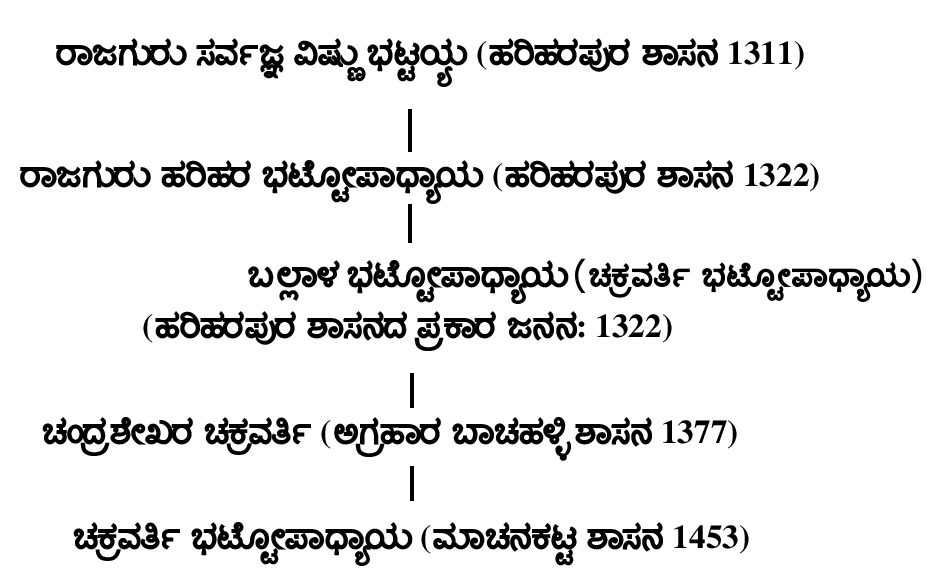
\includegraphics[scale=1.1]{images/chap4/add-chap4fig2.jpeg}
\end{figure}

\textbf{ಯಾದವಗಿರಿಯಾದ ತಿರುನಾರಾಯಣಪುರ\index{ಯಾದವಗಿರಿಯಾದ ತಿರುನಾರಾಯಣಪುರ} \general{\enginline{-}} ತಿರುನಾರಾಯಣಪುರವಾದ ಮೇಲುಕೋಟೆ\index{ತಿರುನಾರಾಯಣಪುರವಾದ ಮೇಲುಕೋಟೆ}:} ಮೇಲುಕೋಟೆಯು ಅಗ್ರಹಾರವಾಗಿತ್ತೇ ಇಲ್ಲವೇ ಎಂಬುದು ಶಾಸನಗಳಿಂದ ಸ್ಪಷ್ಟವಾಗಿ ತಿಳಿದುಬರುವುದಿಲ್ಲ. 14ನೇ ಶತಮಾನಕ್ಕೆ ಸೇರಿದ ಒಂದು ಶಾಸನದಲ್ಲಿ ವೀರಬಲ್ಲಾಳು ಚತುರ್ವೇದಿ ಭಟ್ಟರತ್ನಾಕರವಾದ ನಾಗಮಂಗಲದ ಗಂಗಣ್ಣನು, ಮೇಲುಗೋಟೆಯ ಶೇಷಧರ್ಮ ಮಹಾಜನಗಳಿಗೆ ಯಾವುದೋ ಊರನ್ನು ದತ್ತಿಯಾಗಿ ಬಿಟ್ಟಿದ್ದಾನೆ.\endnote{ ಎಕ 6 ಪಾಂಪು 157 ಮೇಲುಕೋಟೆ 14ನೇ ಶ.} ಮೇಲುಕೋಟೆಯಲ್ಲಿ ಶೇಷಧರ್ಮ ಮಹಾಜನಗಳು\index{ಶೇಷಧರ್ಮ ಮಹಾಜನಗಳು} ಇದ್ದಮೇಲೆ ಅದೊಂದು ಅಗ್ರಹಾರವಾಗಿರಲೇ ಬೇಕು. ಮಾದಪ್ಪ ದಂಡನಾಯಕ\index{ಮಾದಪ್ಪ ದಂಡನಾಯಕ} ಮತ್ತು ಕೇತಪ್ಪ ದಂಡನಾಯಕರ\index{ಕೇತಪ್ಪ ದಂಡನಾಯಕ} ಶಾಸನದಲ್ಲಿ,\endnote{ ಎಕ 6 ಪಾಂಪು 161 ಮೇಲುಕೋಟೆ 14ನೇ ಶ.} ಮತ್ತು ಇದೇ ಮಾದಪ್ಪ ದಂಡನಾಯಕರ ಶಾಸನದಲ್ಲಿ ಅಗ್ರಹಾರದ ಪ್ರಸ್ತಾಪವಿಲ್ಲ.\endnote{ ಎಕ 6 ಪಾಂಪು 185 ಮೇಲುಕೋಟೆ 1319} ಕ್ರಿ.ಶ.1369ರ ಎರಡನೆಯ ಬುಕ್ಕರಾಯನ ಶಾಸನದಲ್ಲಿ “ಶ‍್ರೀಮದನಾದಿ ಮಹಾಸ್ವಾಮಿ ಸಂಸ್ಥಾನಂ\index{ಶ‍್ರೀಮದನಾದಿ ಮಹಾಸ್ವಾಮಿ ಸಂಸ್ಥಾನಂ} ಶ‍್ರೀ ಯಾದವಗಿರಿಯಾದ ತಿರುನಾರಾಯಣ ಪುರದ ಶ‍್ರೀ ವೈಷ್ಣವರು” ಎಂದು ಹೇಳಿದೆ.\endnote{ ಎಕ 6 ಪಾಂಪು 164 ಮೇಲುಕೋಟೆ 1369} ಬಹುತೇಕ ಶಾಸನಗಳಲ್ಲಿ ಯಾದವಗಿರಿಯಾದ ತಿರುನಾರಾಯಣಪುರ ಎಂದೇ ಹೇಳಿದೆ. ಅಗ್ರಹಾರವೆಂದು ಹೇಳಿಲ್ಲ. ಆದುದರಿಂದ ಮೇಲುಕೋಟೆಯ ಶ‍್ರೀವೈಷ್ಣವರ ಆಡಳಿತಕ್ಕೆ ಒಳಪಟ್ಟ ಸ್ವತಂತ್ರವಾದ ಒಂದು ವೈಷ್ಣವ ಕ್ಷೇತ್ರವಾಗಿತೆಂದು ಅಥವಾ ಒಂದು ಪುರವಾಗಿತ್ತೆಂದು ಹೇಳಬಹುದು.

\textbf{ಶ‍್ರೀವೊಪ್ಪಣಾದಿ ಅಗ್ರಹಾರ ಚಿಕ್ಕಅರಸಿನಕೆರೆ\index{ಶ‍್ರೀವೊಪ್ಪಣಾದಿ ಅಗ್ರಹಾರ ಚಿಕ್ಕಅರಸಿನಕೆರೆ}:} ಮದ್ದೂರು ತಾಲ್ಲೂಕು ಕ್ಯಾಗಟ್ಟದ ಹರಿಹರೇಶ್ವರ ದೇವಾಲಯದ\index{ಹರಿಹರೇಶ್ವರ ದೇವಾಲಯ} ಮುಂದಿರುವ ಮುಮ್ಮಡಿ ಬಲ್ಲಾಳನ ಒಂದು ಶಾಸನದಲ್ಲಿ ಚಿಕ್ಕ ಅರಸಿನಕೆರೆಯನ್ನು\index{ಚಿಕ್ಕ ಅರಸಿನಕೆರೆ} `ಶ‍್ರೀ ವೊಪ್ಪಣದಿ ಅಗ್ರಹಾರ' ಎಂದು ಹೇಳಿದೆ. ಈ ಊರಿನ ಮಹಾಜನಗಳು\index{ಮಹಾಜನಗಳು}, ಹಿರಿಯ ಈರೇಗೌಡ, ದೊಡ್ಡಿಯಮ್ಮನ\index{ದೊಡ್ಡಿಯಮ್ಮ} ಮಗಳು ಮರ್ರವಿಗೆ\index{ಮರ್ರವಿ} ಮಾನ್ಯದ ಗದ್ದೆಯನ್ನು ನೀಡಿದರೆಂದು ಹೇಳಿದೆ.\endnote{ ಎಕ 7 ಮ 132 ಕ್ಯಾಗಟ್ಟ 1322}

\textbf{ವಳೈಕುಳವಾದ ಕೊಂಗುಕೊಂಡ ಶ‍್ರೀ ವಿಷ್ಣುವರ್ಧನ ಪೋಸಳ ಚತುರ್ವೇದಿ ಮಂಗಲ(ಬಳಗೊಳ)\index{ವಳೈಕುಳವಾದ ಕೊಂಗುಕೊಂಡ ಶ‍್ರೀ ವಿಷ್ಣುವರ್ಧನ ಪೋಸಳ ಚತುರ್ವೇದಿ ಮಂಗಲ(ಬಳಗೊಳ)}:} ವಳೈಕುಳಮಾನ ಕೊಂಗುಕೊಂಡ ಶ‍್ರೀ ವಿಷ್ಣುವರ್ಧನ ಪೋಸಳ ಚತುರ್ವೇದಿ ಮಂಗಲದ ಶ‍್ರೀಮದಶೇಷ ಮಹಾಜನಗಳು, ಈ ಅಗ್ರಹಾರದಲ್ಲಿ ಶ‍್ರೀಮತ್​ ಸರ್ವನಮಸ್ಯ ಅಗ್ರಹಾರ ದಕ್ಷಿಣ ವಾರಣಾಸಿ ಉದ್ಭವಸರ್ವಜ್ಞಪುರದ\index{ದಕ್ಷಿಣ ವಾರಣಾಸಿ ಉದ್ಭವಸರ್ವಜ್ಞಪುರ} ಇರೈಅಪ್ಪನ್​ ಪ್ರತಿಷ್ಠಾಪಿಸಿದ ರಾಮಲಕ್ಷ್ಮಣ ದೇವರ ತಿರುವಿಡೈಯಾಟ್ಟಕ್ಕೆ (ಕೞನಿ) ಗದ್ದೆಯನ್ನು ಸರ್ವಮಾನ್ಯವಾಗಿ ದತ್ತಿ ಬಿಡುತ್ತಾರೆ. ತಿರುಮಕೂಡಲು ನರಸೀಪುರವೇ\index{ತಿರುಮಕೂಡಲು ನರಸೀಪುರ} ದಕ್ಷಿಣವಾರಣಾಸಿ ಸರ್ವಜ್ಞಪುರ.\endnote{ ಎಕ 6 ಶ‍್ರೀಪ 70 ಬೆಳಗೊಳ 1338} ಈ ಶಾಸನದ ಕಾಲವನ್ನು ಡಾ. ಎಂ.ಎಚ್​. ಕೃಷ್ಣರವರು 1098ಕ್ಕೆ ಸರಿಹೊಂದಿಸಿ, ವಿಷ್ಣುವರ್ಧನನು 1098ರ ರಾಮಾನುಜಾಚಾರ್ಯರನ್ನು\index{ರಾಮಾನುಜಾಚಾರ್ಯರು} ಸಂಧಿಸಿ, ವೈಷ್ಣವಧರ್ಮವನ್ನು ಸ್ವೀಕರಿಸಿ, ವಿಷ್ಣುವರ್ಧನನೆಂಬ ಹೆಸರನ್ನು ಇಟ್ಟುಕೊಂಡನೆಂದು ಹೇಳಿದ್ದಾರೆ. ಈ ಘಟನೆಯು ಸಂಭವಿಸಿದುದು ವೈಷ್ಣವ ಗುರು ಪರಂಪರೆಯ ಪ್ರಕಾರ ಕ್ರಿ.ಶ.1098 ಡಿಸೆಂಬರ್​ 16 ಎಂದು, ಅದಕ್ಕೂ ಒಂದು ತಿಂಗಳ ಮುಂಚೆಯೇ ಈ ಶಾಸನ ಹುಟ್ಟಿದೆ ಎಂದೂ, ವಿಷ್ಣುವರ್ಧನನು ತನ್ನ ಹೆಸರಿನಲ್ಲಿ ಈ ಅಗ್ರಾಹರವನ್ನು ಸ್ಥಾಪಿಸಿದನೆಂದೂ ವಿವರಿಸಿದ್ದಾರೆ. ಆದರೆ ಈ ವಾದವನ್ನು ಒಪ್ಪದ ಡಾ. ಬಾ.ರಾ. ಗೋಪಾಲ್​ ಅವರು ಈ ಶಾಸನವು ಮುಮ್ಮಡಿ ಬಲ್ಲಾಳನ\index{ಮುಮ್ಮಡಿ ಬಲ್ಲಾಳ} ಕಾಲಕ್ಕೆ ಸೇರಿದ್ದೆಂದು ಸಮರ್ಪಕವಾಗಿ ವಿವರಿಸಿದ್ದಾರೆ.\endnote{ ಎಪಿಗ್ರಾಫಿಯಾ ಕರ್ನಾಟಿಕಾ, ಸಂಪುಟ 6, ಪೀಠಿಕೆ, ಪುಟ \engfoot{xliii, xliv}}

\vskip -4pt

\section*{ವಿಜಯನಗರ ಕಾಲದ ಅಗ್ರಹಾರಗಳು}

\vskip -2pt

ಮುಮ್ಮಡಿ ಬಲ್ಲಾಳನ ಕಾಲದಿಂದ ವಿಜಯನಗರದ ಆರಂಭದ ಕಾಲದವರೆಗೆ ಜಿಲ್ಲೆಯಲ್ಲಿ ಅಗ್ರಹಾರದ ಚಟುವಟಿಕೆಗಳಿಗೆ ಸಂಬಂಧಿಸಿದ ಶಾಸನಗಳು ಕಂಡುಬರುವುದಿಲ್ಲ. ಈ ವಿಪ್ಲವ ಕಾಲದಲ್ಲಿ ಅಗ್ರಹಾರದ ಚಟುವಟಿಕೆಗಳು ನಿಂತು ಹೋಗಿದ್ದವೆಂದು ಹೇಳಬಹುದು. ವಿಜಯನಗರದ ಅರಸರು ಹೊಸ ಅಗ್ರಹಾರಗಳನ್ನು ರಚನೆ ಮಾಡಿದುದರ ಜೊತೆಗೆ ಹಳೆಯ ಅಗ್ರಹಾರಗಳನ್ನು ಪುನರುಜ್ಜೀವನಗೊಳಿಸಿರುವುದು ಶಾಸನಗಳ ಅಧ್ಯಯನದಿಂದ ಕಂಡುಬರುತ್ತದೆ. ವಿಜಯನಗರ ಕಾಲದಲ್ಲಿ ಏಕಭೋಗ ದತ್ತಿ ಅಗ್ರಹಾರಗಳು ಕಂಡುಬರುತ್ತವೆ.

\vskip -2pt

\textbf{ಇಮ್ಮಡಿ ಬುಕ್ಕರಾಜಪುರವಾದ ಬಾಚೆಯ ಹಳ್ಳಿ ಅಗ್ರಹಾರ\index{ಇಮ್ಮಡಿ ಬುಕ್ಕರಾಜಪುರವಾದ ಬಾಚೆಯ ಹಳ್ಳಿ ಅಗ್ರಹಾರ}/ ಸಾಯಣ\index{ಸಾಯಣ}, ಮಾಧವರು\index{ಮಾಧವ} ಹಾಗೂ ಅವರ ವಂಶಸ್ಥರು:} ವಿಜಯನಗರ ಸಾಮ್ರಾಜ್ಯದಲ್ಲಿ ಬಹಳ ಪ್ರಮುಖ ಪಾತ್ರವಹಿಸಿದ್ದ ಸಾಯಣ ಮತ್ತು ಮಾಧವ ಹಾಗೂ ಅವರ ವಂಶಸ್ಥರು ದತ್ತಿ ಪಡೆದ ಉಲ್ಲೇಖವಿರುವ, ಕೃಷ್ಣರಾಜಪೇಟೆ\index{ಕೃಷ್ಣರಾಜಪೇಟೆ} ತಾಲ್ಲೂಕು, ಅಗ್ರಹಾರ ಬಾಚಹಳ್ಳಿಯ ತಾಮ್ರಪಟಗಳು ಬಹಳ ಪ್ರಮುಖವೂ,\break ಕುತೂಹಲಕರವೂ ಆಗಿವೆ. ಕೃಷ್ಣರಾಜಪೇಟೆ ತಾಲ್ಲೂಕು ಖಜಾನೆಯಲ್ಲಿ ಬಾಚೆಯಹಳ್ಳಿ ಅಗ್ರಹಾರಕ್ಕೆ ಸಂಬಂಧಿಸಿದ ತಾಮ್ರಪಟಗಳಿವೆ ಎಂದು 1914ರ ಮೈಸೂರು ಆರ್ಕಿಯೋಲಾಜಿಕಲ್​ ರಿಪೋರ್ಟ್‌ನಲ್ಲಿ ಹೇಳಿದ್ದು, ಅದರ ಸಾರಾಂಶವನ್ನು ನೀಡಲಾಗಿದೆ.\endnote{ ಮೈಸೂರು ಆರ್ಕಿಯಾಲಾಜಿಕಲ್​ ರಿಪೊರ್ಟ್, 1914 ಪುಟ 57-58} ಇದು ಐದು ಹಲಗೆಗಳ ತಾಮ್ರಶಾಸನವಾಗಿದ್ದು, ಮೂರನೇ ಹಲಗೆಯ ಮುಂದಿನ ಭಾಗದ ಪಾಠವನ್ನು ಮಾತ್ರ ಎಂ.ಎ.ಆರ್​.ನಲ್ಲಿ ನೀಡಲಾಗಿದೆ.\endnote{ ಅದೇ, ಪುಟ 42} ಮೂಲ ಶಾಸನ ಸಿಗುತ್ತಿಲ್ಲ.

\vskip -2pt

ಒಂದನೇ ಬುಕ್ಕರಾಯ\index{ಒಂದನೇ ಬುಕ್ಕರಾಯ} (1356-77) ಅಥವಾ ಬುಕ್ಕರಾಜನು ಶಕ 1298ನೇ ನಳನಾಮ ಸಂವತ್ಸರದ ಫಾಲ್ಗುಣ ಕೃಷ್ಣಪಕ್ಷದ ಪ್ರತಿಪದೆ ಭೌಮವಾರ (ಕ್ರಿ.ಶ.1377, ಫೆಬ್ರವರಿ 24, ಮಂಗಳವಾರ) ಉತ್ತರಾ ಫಲ್ಗುಣಿ ನಕ್ಷತ್ರದಲ್ಲಿ ಶಿವ\break ಸಾಯುಜ್ಯವನ್ನೈದಿದನೆಂದೂ, ಬುಕ್ಕರಾಜನ ಪಾಪಕ್ಷಯ ದ್ವಾರಾ, ಪರಮೇಶ್ವರ ಪ್ರಸಾದ ಸಿದ್ಯರ್ಥವಾಗಿ, ಅವನ ಮಗ ಹರಿಹರ ಮಹಾರಾಯನು(ಎರಡನೇ ಹರಿಹರ), ಹೋಸಣ ದೇಶದ\index{ಹೋಸಣ ದೇಶ}, ಕಬ್ಬಾಹು ವಿಷಯದ\index{ಕಬ್ಬಾಹು ವಿಷಯ}, ಬಾಚೆಯಹಳ್ಳಿ\index{ಬಾಚೆಯಹಳ್ಳಿ} ಗ್ರಾಮವನ್ನು ಹದಿಮೂರು ಹಳ್ಳಿಗಳ ಸಮೇತ ಇಮ್ಮಡಿ ಬುಕ್ಕರಾಜಪುರವೆಂಬ\index{ಇಮ್ಮಡಿ ಬುಕ್ಕರಾಜಪುರ} ಅಗ್ರಹಾರವನ್ನಾಗಿ ಮಾಡಿ, 60 ವೃತ್ತಿಗಳನ್ನಾಗಿ ವಿಭಾಗಿಸಿ, ನಾನಾಗೋತ್ರದ, ಸೂತ್ರದ ಬ್ರಾಹ್ಮಣರಿಗೆ ದತ್ತಿಯಾಗಿ ಹಾಕಿಕೊಟ್ಟನು. ಪ್ರಕಟಿತ ಮೂರನೆಯ ಹಲಗೆಯ ಪಾಠದದಲ್ಲಿರುವ ಹಳ್ಳಿಗಳು ಹಾಗೂ ಪ್ರತಿಗ್ರಹಿಗಳ ಹೆಸರು ಈ ಕೆಳಗಿನಂತಿದೆ.

\vskip -2pt

ಬಾಚೆಯಹಳ್ಳಿ ಗ್ರಾಮವನ್ನು ಹಾಗೂ ದಂಡೆ ಮತಿಘಟ್ಟಕ್ಕೆ\index{ದಂಡೆ ಮತಿಘಟ್ಟ} ಸೇರಿದ್ದ, ಚಿಕ್ಕಮತಿಘಟ್ಟ, ಬೊಮ್ಮನಾಯಕನಹಳ್ಳಿ, ಶೂನ್ಯಗ್ರಾಮ ತಡಿಕಟ್ಟ(ಬೇಚಿರಾಕ್​), ಈ ಮೂರು ಗ್ರಾಮಗಳ ಸಹಿತ, ಈ ಗ್ರಾಮಗಳಿಗೆ ಸೇರಿದ ಹದಿಮೂರು ಕಾಲುವಳ್ಳಿಗಳ ಸಮೇತ (ಬೆಳಗೊಳ ಬೆಟ್ಟದ ನಾಗಮ ಪಲ್ಲಿ, ಚಾಕ ಪಲ್ಲಿ, ಉಯ್ಯಪಲ್ಲಿ, ಹಿರಿಯಮಾದನ ಪಲ್ಲಿ, ಬೊಪ್ಪನ ಪಲ್ಲಿ, ಕಾಲ ಪಲ್ಲಿ, ಬಡಿವ ಪಲ್ಲಿ, ಕೋಪನ ಪಲ್ಲಿ, ಹರಿಯನ ಪಲ್ಲಿ, ಚಿಲದ ಪಲ್ಲಿ, ಶೂನ್ಯ ಗ್ರಾಮ ಅವ್ವೆಯ ಪಲ್ಲಿ, ಕಣಿಯನ ಪಲ್ಲಿ, ಬನ್ನ ಪಲ್ಲಿ) ಇವೇ ಆ ಹಳ್ಳಿಗಳು. ಅಗ್ರಹಾರಬಾಚ ಹಳ್ಳಿಯ ಸುತ್ತಮುತ್ತ ಈಗಲೂ ಇರುವ, ಬೊಮ್ಮನಾಯಕನ ಹಳ್ಳಿ\index{ಬೊಮ್ಮನಾಯಕನ ಹಳ್ಳಿ}, ಉಯ್ಯಗೋನ ಹಳ್ಳಿ, ಮಾದಿ ಹಳ್ಳಿ, ಚಾಕನ ಹಳ್ಳಿ, ಅರೆಬೊಪ್ಪನ ಹಳ್ಳಿ\index{ಅರೆಬೊಪ್ಪನ ಹಳ್ಳಿ}, ಕಾಳೇನ ಹಳ್ಳಿ, ಬಂಡಬೋಯನ ಹಳ್ಳಿ\index{ಬಂಡಬೋಯನ ಹಳ್ಳಿ}, ಹರಿನ ಹಳ್ಳಿ, ಚಿಲ್ಲದ ಹಳ್ಳಿ, ಬಣ್ಣೇನ ಹಳ್ಳಿ, ಮತ್ತಿಘಟ್ಟ, ಇವುಗಳನ್ನು ಗುರುತಿಸಬಹದು. ಬೆಳಗೊಳ ಬೆಟ್ಟದ ಹಿಂದೆ ನಾಗಯ್ಯನ ಕೊಪ್ಪಲು\index{ನಾಗಯ್ಯನ ಕೊಪ್ಪಲು} ಗ್ರಾಮವಿದೆ.

\vskip -2pt

ಪ್ರತಿಗ್ರಹಿಗಳ ಪೈಕಿ, ಭಾರದ್ವಾಜಗೋತ್ರದ, ಯಜುಶ್ಶಾಖೆಯ, ಸಾಯಣಾಚಾರ್ಯ\index{ಸಾಯಣಾಚಾರ್ಯ}, ಅವರ ಮಗ ಸಿಂಗಣ\index{ಸಿಂಗಣ}, ಮಾಧವಾಚಾರ್ಯನ\index{ಮಾಧವಾಚಾರ್ಯ} ತನುಜ ಮಾಯಣ\index{ಮಾಯಣ}, ಸಾಯಣಾರ್ಯ ತನೂಜ ಮಾದಣ\index{ಮಾದಣ}, ನಾಗಣ\index{ನಾಗಣ}, ಹರಿತ ಗೋತ್ರದ ತಾರ್ಕಿಕ ಭಟ್ಟ\index{ತಾರ್ಕಿಕ ಭಟ್ಟ}, ಆತ್ರೇಯ ಗೋತ್ರದ ಚಿನ್ಮಯಭಟ್ಟ\index{ಚಿನ್ಮಯಭಟ್ಟ}, ಭಾರದ್ವಾಜ ಗೋತ್ರದ ಚಂದ್ರಶೇಖರ ಚಕ್ರವರ್ತಿ\index{ಚಂದ್ರಶೇಖರ ಚಕ್ರವರ್ತಿ}, ಅವನ ಮಗ ನರಹರಿಭಟ್ಟ, ಗೌತಮ ಗೋತ್ರದ ಜನಾರ್ದನ ಭಟ್ಟ\index{ಜನಾರ್ದನ ಭಟ್ಟ}, ಭಾರದ್ವಾಜ ಗೋತ್ರದ ಕಂದರ್ಪದೀಕ್ಷಿತ\index{ಕಂದರ್ಪದೀಕ್ಷಿತ}, ಭಾರದ್ವಾಜ ಗೋತ್ರದ ಅಣ್ಣದೀಕ್ಷಿತ\index{ಅಣ್ಣದೀಕ್ಷಿತ}, ಗಾರ್ಗ್ಯ ಗೋತ್ರದ ವರಾಹದೀಕ್ಷಿತ\index{ವರಾಹದೀಕ್ಷಿತ}, ವಿಶ್ವಾಮಿತ್ರ ಗೋತ್ರದ ಅಪ್ಪದೇವ ದೀಕ್ಷಿತ\index{ಅಪ್ಪದೇವ ದೀಕ್ಷಿತ}, ಕೌಶಿಕ ಗೋತ್ರದ ನರಸಿಂಹ ದೀಕ್ಷಿತ\index{ನರಸಿಂಹ ದೀಕ್ಷಿತ} ಇವರುಗಳ ಹೆಸರುಗಳು ಮಾತ್ರ ವರದಿಯಲ್ಲಿ ಪ್ರಕಟಿಸಿರುವ ಮೂರನೆಯ ಹಲಗೆಯಿಂದ ತಿಳಿದುಬರುತ್ತದೆ.

ಡಿ.ವಿ.ಜಿ. ಅವರು ‘ವಿದ್ಯಾರಣ್ಯರ ಸಮಕಾಲೀನರು\index{ವಿದ್ಯಾರಣ್ಯರ ಸಮಕಾಲೀನರು}’ ಕೃತಿಯಲ್ಲಿ ಈ ತಾಮ್ರಪಟದ ವಿಷಯವನ್ನು ಪ್ರಸ್ತಾಪಿಸಿ, ಕೆಲವು ವಿವರಗಳನ್ನು ನೀಡಿದ್ದಾರೆ. ಅಗ್ರಹಾರದ ಹಳ್ಳಿಗಳ ಹೆಸರನ್ನು ನೀಡಿರುವುದಿಲ್ಲ. ಆದರೆ ಪ್ರತಿಗ್ರಹಿಗಳ ಬಗ್ಗೆ ಕೆಲವು ವಿಚಾರಗಳನ್ನು ಪ್ರಸ್ತಾಪಿಸಿದ್ದಾರೆ.\endnote{ ಡಿವಿಜಿ ಕೃತಿ ಶ್ರೇಣಿ, ವಿದ್ಯಾರಣ್ಯರ ಸಮಕಾಲೀನರು, ಪುಟ 349-50} ಎ.ವಿ. ವೆಂಕಟರತ್ನಂ ಅವರು ಈ ವಿಷಯವನ್ನು ಪ್ರಸ್ತಾಪಿಸಿದ್ದಾರೆ. ಆದರೆ ಅಗ್ರಹಾರಕ್ಕೆ ಸೇರಿದ ಹಳ್ಳಿಗಳ ಹೆಸರು ಹಾಗೂ ಪ್ರತಿಗ್ರಹಿಗಳ ಹೆಸರನ್ನು ಉಲ್ಲೇಖಿಸಿರುವುದಿಲ್ಲ.\endnote{ Venkataratnam, Dr.A.V. Local Government in the Vijayanagara Empire, pp.47 (MAR 1914, pp.57-58)} ಶತಾವಧಾನಿ ಡಾ. ಆರ್​. ಗಣೇಶ್​ ಅವರು ತಮ್ಮ ‘ವಿಭೂತಿ ಪುರುಷ ವಿದ್ಯಾರಣ್ಯರು’ ಕೃತಿಯಲ್ಲಿ ಈ ಶಾಸನದ ಬಗ್ಗೆ ಪ್ರಸ್ತಾಪಿಸಿಲ್ಲ.

"ರಾಯಸಮುದ್ರದ ಎಂಟುಮೈಲಿ ಉತ್ತರಕ್ಕಿರುವ ಅಗ್ರಹಾರಬಾಚೆಯಹಳ್ಳಿ ಮತ್ತು ಅದರ ಸುತ್ತ ಮುತ್ತಿನ ಹದಿಮೂರು ಹಳ್ಳಿಗಳನ್ನು ಪ್ರಸಿದ್ಧ ವೇದ ಭಾಷ್ಯಕಾರರಾದ ಸಾಯಣಾಚಾರ್ಯನಿಗೆ ದತ್ತಿಯಾಗಿ ಕೊಟ್ಟಿತ್ತು, ಅದಕ್ಕೆ ಆಗ ಇಮ್ಮಡಿ ಬುಕ್ಕರಾಜಪುರ\-ವೆಂಬ ಹೆಸರು. ಸಿಂದಘಟ್ಟದಿಂದ ನೈರುತ್ಯಕ್ಕೆ 10-12 ಮೈಲಿ ದೂರವಿರುವ ಹರಿಹರಪುರವನ್ನು, ಹರಿಹರ ಭಟ್ಟನೆಂಬುವವನಿಗೆ\index{ಹರಿಹರ ಭಟ್ಟ} ದತ್ತಿಯಾಗಿ ಕೊಟ್ಟಿತ್ತು. ಈತನು ವೇದ ವೇದಾಂಗ ಪಾರಗನೂ ಸಾಯಣಾಚಾರ್ಯನ ವೇದಗುರುವೂ ಆದ ಕಂಚಿಯ ವಿಷ್ಣುಭಟ್ಟನ\index{ಕಂಚಿಯ ವಿಷ್ಣುಭಟ್ಟ} ಮಗನಿರಬೇಕು" ಎಂದು ಸಿ.ಜೆ. ಪುರುಷೋತ್ತಮ್ ಅವರು ಹೇಳಿದ್ದಾರೆ.\endnote{ ಪುರುಷೋತ್ತಮ, ಸಿ.ಜೆ, ಸಿಂಧಘಟ್ಟದ ಶಾಸನ, ಇಕ್ಷುಕಾವೇರಿ, ಪುಟ 119 (ಮೈಸೂರ್​ ಆರ್ಕಿಯಾಲಾಜಿಕಲ್​ ರಿಪೋರ್ಟ್, 1914-15, ಪುಟ 42)}

ಕ್ರಿ.ಶ.1722ರ ಕೃಷ್ಣರಾಜೊಡೆಯರ ತೊಣ್ಣೂರು\index{ತೊಣ್ಣೂರು} ತಾಮ್ರಶಾಸನದಲ್ಲಿ ಚೆಲುವದೇವಾಂಬುಧಿ ಅಗ್ರಹಾರದ(ಅತ್ತಿಗುಪ್ಪೆ)\index{ಚೆಲುವದೇವಾಂಬುಧಿ ಅಗ್ರಹಾರದ(ಅತ್ತಿಗುಪ್ಪೆ)} ಈಶಾನ್ಯಕ್ಕೆ ಬಾಚಹಳ್ಳಿ ಅಗ್ರಹಾರವಿತ್ತೆಂದೂ, ಅದಕ್ಕೆ ಬಂಡಮಾರನಹಳ್ಳಿ ಗ್ರಾಮವು ಸೇರಿತ್ತೆಂದು ಹೇಳಿದೆ.\endnote{ ಎಕ 6 ಪಾಂಪು 99 ತೊಣ್ಣೂರು 1722} ಇದರಿಂದ ಬಾಚೆಯಹಳ್ಳಿ ಅಗ್ರಹಾರವು ಕ್ರಿ.ಶ.1377 ರಿಂದ 1722ರವರೆಗೂ ಅಸ್ತಿತ್ವದಲ್ಲಿತ್ತೆಂದು ತಿಳಿದುಬರುತ್ತದೆ. ಆದರೆ ಈ ಊರಿನಲ್ಲಿ ಈಗ ಕೇವಲ ಒಂದು ಅಥವಾ ಎರಡು ಬ್ರಾಹ್ಮಣರ ಮನೆಗಳಿವೆ.

ಮೊದಲನೆಯದಾಗಿ ಕ್ರಿ.ಶ. 1410ರ ಹಂಪೆಯ ಲಕ್ಷ್ಮೀಧರ ಅಮಾತ್ಯನ\index{ಲಕ್ಷ್ಮೀಧರ ಅಮಾತ್ಯ} ಶಾಸನದಲ್ಲಿ ಬರುವ ಸಾಯಣ ಮತ್ತು ಮಾಧವರ ವಂಶಾವಳಿಯು ಕೆಳಗಿನಂತಿದೆ.\endnote{ ಕ ವಿ ವಿ, ಶಾಸನ ಸಂಪುಟ 3, ಹಂಪಿ ಶಾಸನಗಳು 69, ಕ್ರಿ.ಶ.1410 ಕಡಲೆಕಾಳು ಗಣೇಶನಗುಡಿ ಮುಂದೆ} ಈ ಶಾಸನದಲ್ಲಿ ಇವರು ಕಂನಡಿಗ ಕುಲದವರೆಂದು\index{ಕಂನಡಿಗ ಕುಲ} ಹೇಳಿದ್ದು, ಸಾಯಣ ಮಾಧವರ ತಂದೆ ತಾಯಿಗಳು ಅಥವಾ ಊರಿನ ಹೆಸರನ್ನು ಉಲ್ಲೇಖಿಸಿಲ್ಲ.

\begin{figure}[H]
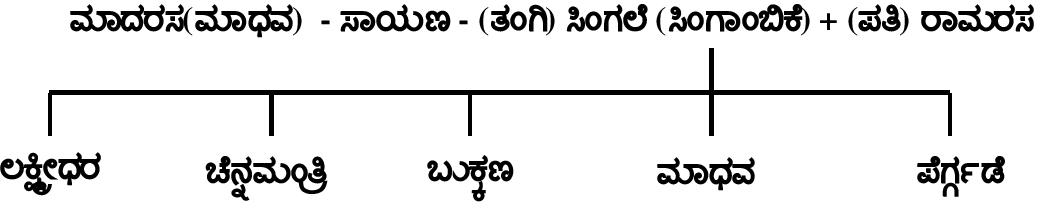
\includegraphics[scale=1.1]{images/chap4/add-chap4fig3.jpeg}
\end{figure}

ಕಂಚಿ ವರದರಾಜಸ್ವಾಮಿ ದೇವಾಲಯದ ಅಭಿಷೇಕ ಮಂಟಪದ ಶಾಸನದಲ್ಲಿ ಶ‍್ರೀಮತಿ\index{ಶ‍್ರೀಮತಿ} ಮತ್ತು ಮಾಯಣರ\index{ಮಾಯಣರ} ಪುತ್ರ, ಸಾಯಣ, ಭೋಗನಾಥ, ಸಿಂಗಲೆ ಇವರ ಅಣ್ಣನೇ ಮಾಧವನೆಂದೂ ಇವನು ಸಂಗಮ ಭೂಪತಿಯ ಆಶ್ರಯದಲ್ಲಿದ್ದನೆಂದೂ, ಇವನ ಗುರು ಶ‍್ರೀಕಂಠನಾಥನೆಂದೂ ಹೇಳಿದೆ.\endnote{ ಲಕ್ಷ್ಮೀನರಸಿಂಹ ಶಾಸ್ತ್ರಿ ಹುರಗಲವಾಡಿ, ವಿಜಯನಗರ ಸಾಮ್ರಾಜ್ಯ ಸ್ಥಾಪಕ ವಿದ್ಯಾರಣ್ಯರು, ಪುಟ 3} ಸಾಯಣನ ಹಿರಿಯ ಸಹೋದರ ಮಾಧವಾಚಾರ್ಯನು ರಚಿಸಿರುವ\break ‘ಪರಾಶರ ಸ್ಮೃತಿ’ (ಪರಾಶರ ಮಾಧವೀಯ)\index{ಪರಾಶರ ಸ್ಮೃತಿ (ಪರಾಶರ ಮಾಧವೀಯ)} ಕೃತಿಯಲ್ಲೂ ಕೂಡಾ, ಸಾಯಣನ ತಂದೆ ತಾಯಿಗಳು ಮಾಯಣ ಮತ್ತು ಶ‍್ರೀಮತಿ ಎಂದೂ, ಸಾಯಣನಿಗೆ ಕಂಪಣ, ಮಾಯಣ ಮತ್ತು ಸಿಂಗಣ ಎಂಬ ಮೂರು ಜನ ಮಕ್ಕಳಿದ್ದರೆಂದೂ ಹೇಳಿದೆ.\break ಸಾಯಣನ ಅಲಂಕಾರ ಸುಧಾನಿಧಿಯಲ್ಲೂ ಸಾಯಣನಿಗೆ ಕಂಪಣ, ಮಾಯಣ ಮತ್ತು ಸಿಂಗಣ ಎಂಬ ಮೂರು ಜನ ಮಕ್ಕಳಿದ್ದರೆಂದು ಹೇಳಿದೆ.\endnote{ ಗಡಿಯಾರಂ ರಾಮಕೃಷ್ಣ ಶರ್ಮ, ವಿದ್ಯಾರಣ್ಯರು-ಒಂದು ಚಾರಿತ್ರಿಕ ಅಧ್ಯಯನ, ಅನು: ರಾಮಚಂದ್ರರಾವ್​ ಗುಮಾಸ್ತೆ, ಪುಟ 87} ಸಾಯಣನಿಗೆ ಮೇಲಿನಂತೆ ಮೂರು ಜನ ಮಕ್ಕಳಿದ್ದರೆಂದೂ, ಅವನ ಹೆಂಡತಿಯ ಹೆಸರು ಹೇಮಾವತಿ ಎಂದು ಮೋಡಕ್​ ಅವರು ಹೇಳಿದ್ದಾರೆ.\endnote{ Modak, B.R, Sayana, pp.27} ಸಾಯಣನು ಮೊದಲನೇ ಹರಿಹರನ ಕಾಲದಲ್ಲಿ ‘ವೇದಾರ್ಥ ಪ್ರಕಾಶ’ ಎಂಬ ವೇದ ಭಾಷ್ಯ ಕೃತಿಯನ್ನು ರಚಿಸಿದನು.\endnote{ ಇಮ್ಮಡಿ ಶಿವಬಸವ ಸ್ವಾಮಿಗಳು, ಸಂಸ್ಕೃತ ಸಾಹಿತ್ಯಕ್ಕೆ ಕರ್ನಾಟಕದ ಕೊಡುಗೆ, ಪುಟ 286 ಡಿವಿಜಿ ಕೃತಿ ಶ್ರೇಣಿ,

ಸಂಪುಟ, 4, ವಿದ್ಯಾರಣ್ಯರ ಸಮಕಾಲೀನರು, ಪುಟ 385} ಸಾಯಣ\index{ಸಾಯಣ}, ಮಾಧವ\index{ಮಾಧವ}, ಭೋಗನಾಥ\index{ಭೋಗನಾಥ} ಇವರ ಗುರುಗಳು ಶ‍್ರೀಕಂಠನಾಥರೆಂದು\index{ಶ‍್ರೀಕಂಠನಾಥ} ಪರಾಶರ ಮಾಧವೀಯ ಮತ್ತು ಭೋಗನಾಥನ ‘ಮಹಾಗಣಪತಿ ಸ್ತವ’ದಲ್ಲಿ ಉಲ್ಲೇಖವಾಗಿದೆ.\endnote{ ಡಿವಿಜಿ ಕೃತಿ ಶ್ರೇಣಿ, ಸಂಪುಟ 4, ವಿದ್ಯಾರಣ್ಯರು ಮತ್ತು ಅವರ ಕಾಲ, ಪುಟ 234} ಭಾರದ್ವಾಜ ಗೋತ್ರದ, ಮಾಧವ ಅಮಾತ್ಯನ ಮಗ ಶಶಧರನು\index{ಶಶಧರ} ವಿರೂಪಾಕ್ಷ ದೇವರಿಗೆ ದೀಪಸ್ಥಂಭವನ್ನು ಮಾಡಿಸಿದ್ದನೆಂದೂ, ಅದನ್ನು ಅವನ ಮಗ\break ಮಾದಣಮಾತ್ಯನು ದೇವರಿಗೆ ಸಮರ್ಪಿಸಿದನೆಂದೂ ವಿರೂಪಾಕ್ಷ ದೇವರ ಗುಡಿ ದ್ವಾರದ ಬಳಿ ಇರುವ ದೀಪದ ಕಂಬದ ಮೇಲಿನ ಶಾಸನದಿಂದ ತಿಳಿದು ಬರುತ್ತದೆ.\endnote{ ಕನ್ನಡ ವಿ.ವಿ. ಶಾಸನ ಸಂಪುಟ-3, ಹಂಪಿ 30, ಕ್ರಿ.ಶ.1428} ಮೇಲ್ಕಂಡ ಉಲ್ಲೇಖಗಳ ಪ್ರಕಾರ ಸಾಯಣ ಮಾಧವರ ವಂಶವೃಕ್ಷದ ಎರಡನೇ ಹಂತವನ್ನು ಈ ರೀತಿ ಕಟ್ಟಿಕೊಡಬಹುದು.

\begin{figure}[H]
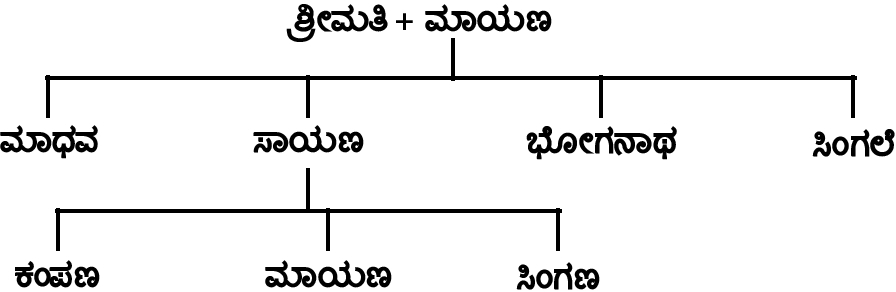
\includegraphics[scale=1.05]{images/chap4/add-chap4fig4.jpeg}
\end{figure}

ಮೇಲೆ ಉಲ್ಲೇಖಿಸಿದ ಬಾಚೆಯಹಳ್ಳಿ (ಅಗ್ರಹಾರ ಬಾಚಹಳ್ಳಿ)\index{ಬಾಚೆಯಹಳ್ಳಿ (ಅಗ್ರಹಾರ ಬಾಚಹಳ್ಳಿ)} ತಾಮ್ರ ಪಟಗಳು ಮತ್ತು ಹಂಪಿಯ ವಿರೂಪಾಕ್ಷ ದೇವಾಲಯ ದೀಪದ ಕಂಬದ ಮೇಲಿನ ಶಾಸನದ ಪ್ರಕಾರ ತಿಳಿದು ಬರುವ ಸಾಯಣ ಮತ್ತು ಮಾಧವರ ವಂಶಾವಳಿಯನ್ನು ಈ ಕೆಳಗಿನಂತೆ ನೀಡಬಹುದು.

\begin{figure}[H]
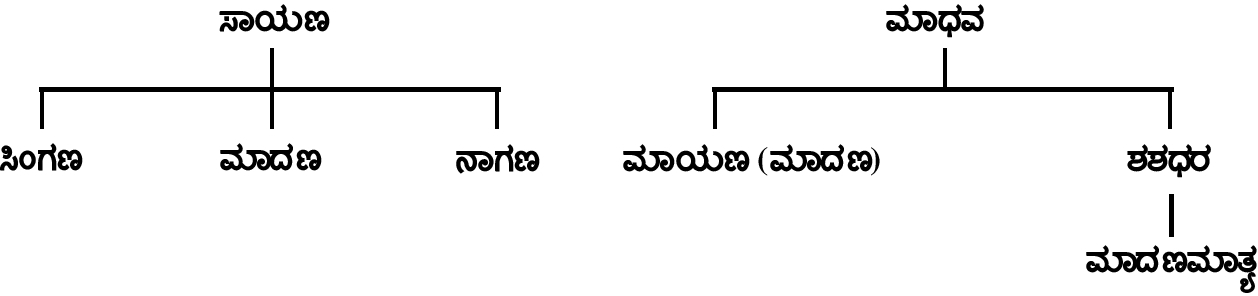
\includegraphics[scale=1.05]{images/chap4/add-chap4fig5.jpeg}
\end{figure}

ಪೂರ್ವೋಕ್ತ ಪರಾಶರ ಮಾಧವೀಯದ ಉಲ್ಲೇಖದ ಪ್ರಕಾರ ಸಾಯಣಾಚಾರ್ಯನಿಗೆ ಕಂಪಣ, ಮಾಯಣ ಮತ್ತು ಸಿಂಗಣ ಎಂಬ ಮೂವರು ಮಕ್ಕಳಿದ್ದರು. ಆದರೆ ಬಾಚೆಯಹಳ್ಳಿ ಶಾಸನದ ಪ್ರಕಾರ ಸಾಯಣಾಚಾರ್ಯನಿಗೆ ಸಿಂಗಣ, ಮಾದಣ ಮತ್ತು ನಾಗಣ ಎಂಬ ಮೂವರು ಮಕ್ಕಳಿದ್ದರೆಂದು ತಿಳಿದು ಬರುತ್ತದೆ. ಮಾಯಣ, ಮಾದಣ ಎರಡೂ ಒಂದೇ ಹೆಸರೆಂದು ಹೇಳಬಹುದು. “ಕಾಂಚೀಪುರದ ಶಾಸನದಲ್ಲಿ ಮಾಧವಾಚಾರ್ಯ\index{ಮಾಧವಾಚಾರ್ಯ} ಮತ್ತು ಆತನ ಸಹೋದರರು ಹಾಗೂ ಆತನ\break ಆಶ್ರಯದಾತರನ್ನು ಉಲ್ಲೇಖಿಸುವಾಗ ಮಾಧವನಿಗೆ ಮಾಯಣ ಎಂದಿರುವುದು ಗಮನಾರ್ಹ. ಆರ್​. ನರಸಿಂಹಾಚಾರ್ಯರೂ ಸಾಯಣನ ಮಗನಾದ ಮಾಧವನೇ ಸರ್ವದರ್ಶನ ಸಂಗ್ರಹವನ್ನು\index{ಸರ್ವದರ್ಶನ ಸಂಗ್ರಹ} ರಚಿಸಿದವನು ಎಂದು ಹೇಳಿದ್ದಾರೆ. ಇವರ ಅಭಿಪ್ರಾಯ\-ದಂತೆ ಮಾಯಣ ಎಂಬುದು ಮಾಧವ ಎಂಬುದರ ಅಪಭ್ರಂಶ” ಎಂದು ಇಮ್ಮಡಿ ಶಿವಬಸವಸ್ವಾಮಿಗಳು ವಿವರಿಸಿದ್ದಾರೆ.\endnote{ ಇಮ್ಮಡಿ ಶಿವಬಸವ ಸ್ವಾಮಿಗಳು, ಸರ್ವದರ್ಶನ ಸಂಗ್ರಹ, ಪ್ರಸ್ತಾವನೆ, ಪುಟ xxxi} ಆದರೆ ಸಾಯಣನಿಗೆ ನಾಗಣ ಎಂಬ ಇನ್ನೊಬ್ಬ ಮಗನಿದ್ದನೆಂದು ಹೇಳಬೇಕಾಗುತ್ತದೆ. ಬುಕ್ಕರಾಯನ ಮಗ ಕಂಪಣನು ಸಾಯಣನ\break ಆಶ್ರಯದಾತನಾಗಿದ್ದರಿಂದ, ನಾಗಣನಿಗೆ ಕಂಪಣನೆಂಬ ಹೆಸರೂ ಇತ್ತು ಎಂದರೆ ಸಮಸ್ಯೆ ಬಗೆ ಹರಿಯುತ್ತದೆ.

ಬಾಚಹಳ್ಳಿ ಶಾಸನೋಕ್ತ ಮಾಧವ ಮತ್ತು ಅವನ ಮಗ ಮಾಯಣ ಯಾರು ಎಂಬುದು ಪ್ರಶ್ನೆಯಾಗಿ ಉಳಿಯುತ್ತದೆ. ಪೂರ್ವೋಕ್ತ ಹಂಪೆಯ ಶಾಸನದಲ್ಲಿ ಭಾರದ್ವಾಜ ಗೋತ್ರದ ಮಾಧವನಿಗೆ ಶಶಧರನೆಂಬ ಮಗನಿದ್ದನೆಂದು ಹೇಳಿದೆ.\break ಮಾಧವಾಚಾರ್ಯರು 1333ರಲ್ಲಿ ಸನ್ಯಾಸಾಶ್ರಮವನ್ನು ಸ್ವೀಕರಿಸಿ ವಿದ್ಯಾರಣ್ಯರೆಂಬ\index{ವಿದ್ಯಾರಣ್ಯ} ಹೆಸರಿನಿಂದ ಶೃಂಗೇರಿ ಪೀಠಾಧಿಪತಿ\-ಗಳಾದರೆಂಬ ಊಹೆ ಪ್ರಬಲವಾಗಿದೆ.\endnote{ ಗಡಿಯಾರಂ ರಾಮಕೃಷ್ಣ ಶರ್ಮ, ವಿದ್ಯಾರಣ್ಯರು-ಒಂದು ಚಾರಿತ್ರಿಕ ಅಧ್ಯಯನ, ಅನು: ರಾಮಚಂದ್ರ ಗುಮಾಸ್ತೆ, ಪುಟ 42} ಮಾಧವಾಚಾರ್ಯರು ಶೃಂಗೇರಿ ಪೀಠಾಧಿಪತಿಗಳಾಗುವುದಕ್ಕೆ ಮುಂಚೆ ಗೃಹಸ್ಥರಾಗಿದ್ದರು ಎಂದು ವಿದ್ವಾಂಸರು ಹೇಳಿದ್ದಾರೆ.\endnote{ ಕೃಷ್ಣಮೂರ್ತಿ, ಕೆ. ಡಾ. ಮಾಧವ ವಿದ್ಯಾರಣ್ಯರು ಒಬ್ಬರೇ, ಸಂಗಮರ ಕಾಲದ ವಿಜಯನಗರ, ಪುಟ 40} ಮಾಧವಾಚಾರ್ಯರು ಗೃಹಸ್ಥಾಶ್ರಮವನ್ನು ಸ್ವೀಕರಿಸಿದ್ದರೆಂದೂ, ಅವರಿಗೆ ಸೋಮೇಶ್ವರ ಭಟ್ಟನೆಂಬ ಪುತ್ರನಿದ್ದನೆಂದೂ ತಿಳಿದುಬರುತ್ತದೆ.\endnote{ ಶತಾವಧಾನಿ ಡಾ.ಆರ್​.ಗಣೇಶ್​, ವಿಭೂತಿಪುರುಷ ವಿದ್ಯಾರಣ್ಯ, ಪುಟ 29} ಹಂಪೆ ಶಾಸನೋಕ್ತ ಶಶಧರನೇ ಸೋಮೇಶ್ವರ ಭಟ್ಟನಿರಬಹುದೆಂದು ಊಹಿಸಬಹುದು. ಆದರೆ ಡಿ.ವಿ.ಜಿ.ಯವರು, ಬಾಚೆಯಹಳ್ಳಿ ತಾಮ್ರ ಶಾಸನದಲ್ಲಿ ಮೊದಲಿಗೆ ಸಾಯಣಾಚಾರ್ಯನ ಹೆಸರನ್ನು ನೀಡಿ ನಂತರ ಮಾಧವಾಚಾರ್ಯನ ಹೆಸರನ್ನು ನೀಡಲಾಗಿದೆ. ಮಾಧವಾಚಾರ್ಯನು, ಸಾಯಣಾಚಾರ್ಯನ ಅಣ್ಣ\-ನಾಗಿದ್ದರೆ, ಮೊದಲೇ ಅವನ ಹೆಸರು ಉಲ್ಲೇಖವಾಗಬೇಕಾಗಿತ್ತು. ಪ್ರಸ್ತುತ ಶಾಸನ ಕಾಲಕ್ಕಾಗಲೇ ಮಾಧವಾಚಾರ್ಯರು ಬ್ರಹ್ಮಚರ್ಯದಿಂದ ಸಂನ್ಯಸ್ತರಾಗಿ ವಿದ್ಯಾರಣ್ಯ ನಾಮಧೇಯದಿಂದ ಜಗದ್ವಿಖ್ಯಾತರಾಗಿದ್ದರು. ಆದಕಾರಣ ಶಾಸನೋಕ್ತ ಮಾಧವನು(ಮಾದಣ್ಣ), ಮಾಧವಾಚಾರ್ಯರ ಸಹೋದರಿ, ಸಿಂಗಲೆಯ ಮಗ, ಸಾಯಣ ಮಾಧವರ ಸೋದರಳಿಯ, ಮಾಧವನೆಂದು ಹೇಳಿದ್ದಾರೆ. ಆದರೆ ಸಿಂಗಲೆಯ\index{ಸಿಂಗಲೆ} ಪತಿ ರಾಮರಸನು\index{ರಾಮರಸ} ವಿಷ್ಣುವೃದ್ಧ ಗೋತ್ರದವನಾಗಿದ್ದಾನೆ\index{ವಿಷ್ಣುವೃದ್ಧ ಗೋತ್ರ}. ಪೂರ್ವೋಕ್ತ ಹಂಪೆಯ ಶಾಸನದಲ್ಲಿ ಭಾರದ್ವಾಜ ಗೋತ್ರದ ಮಾಧವನ ಮಗ ಶಶಧರ\index{ಶಶಧರ} ಎಂದು ಹೇಳಿರುವುದು ಸಂದೇಹಕ್ಕೆಡೆ ಮಾಡಿಕೊಡುತ್ತದೆ.

ಸಾಯಣ, ಮಾಧವ ಮತ್ತು ಅವರ ವಂಶದವರು, ಈ ಬಾಚೆಯಹಳ್ಳಿಯನ್ನೇ ವೃತ್ತಿಯನ್ನಾಗಿ ಪಡೆಯಲು ಕಾರಣ\-ಗಳೇನು ಎಂಬುದರ ಬಗ್ಗೆ ವಿವೇಚಿಸಿದಾಗ, ಅವು ಇದೇ ಭಾಗದವರು ಅಥವಾ ಈ ಊರಿನವರೇ ಆಗಿರಬಹುದೆಂದು ಸಾಮಾನ್ಯವಾಗಿ ಊಹಿಸಬಹುದು. ಸಾಯಣಾಚಾರ್ಯನ ಪುತ್ರ ಮಾಧವನು ತನ್ನ ಸರ್ವದರ್ಶನ ಸಂಗ್ರಹದ ಆರಂಭದಲ್ಲಿ ಸರ್ವಜ್ಞ ವಿಷ್ಣುವು ತನ್ನ ಗುರುವೆಂದು ಹೇಳಿ ಸ್ತುತಿಸಿದ್ದಾನೆ. ಸರ್ವಜ್ಞ ವಿಷ್ಣು ಅಥವಾ ಸರ್ವಜ್ಞ ವಿಷ್ಣು ಭಟ್ಟಯ್ಯನು\index{ಸರ್ವಜ್ಞ ವಿಷ್ಣು ಭಟ್ಟಯ್ಯ} ಹರಿಹರಪುರ\index{ಹರಿಹರಪುರ} ಅಗ್ರಹಾರದವನಾಗಿದ್ದರಿಂದ, ಸಾಯಣ ಮಾಧವ ಹಾಗೂ ಅವರ ವಂಶಸ್ಥರು ಈ ಕಡೆಯವರೇ ಆಗಿದ್ದು, ಅವರು ತಮ್ಮ\break ಸ್ವಸ್ಥಾನಕ್ಕೆ ಬಂದು ನೆಲೆಸಿದರೆಂದು ಹೇಳಬಹುದು. ಅಗ್ರಹಾರ ಬಾಚಹಳ್ಳಿಯಲ್ಲಿ ಶಂಕರಾಚಾರ್ಯರ ಪರಂಪರೆಗೆ ಸೇರಿದ\break ಅಯ್ಯರ್​(ದ್ರಾವಿಡ ಬೃಹಚ್ಛರಣ) ಬ್ರಾಹ್ಮಣರೂ ಹೆಚ್ಚಿನ ಸಂಖ್ಯೆಯಲ್ಲಿ ನೆಲೆಸಿದ್ದರು. ಈಗ ಆ ಊರಿನಲ್ಲಿ ಒಂದೇ ಒಂದು\break ಕುಟುಂಬವಿದೆ. ಇವರೆಲ್ಲಾ ಶಂಕರಾಚಾರ್ಯರ ಜೊತೆಯಲ್ಲಿ ಕನ್ನಡ ನಾಡಿಗೆ ಬಂದು, ಕೊನೆಗೆ ಸಾಯಣ ಮಾಧವರ ಜೊತೆಗೆ\break ಅಗ್ರಹಾರಬಾಚಹಳ್ಳಿಗೆ ಬಂದು ನೆಲೆಸಿದರೆಂದು ಊಹಿಸಬಹುದು. ಅಗ್ರಹಾರಬಾಚಹಳ್ಳಿಗೆ ಸಮೀಪದಲ್ಲಿ ಭಾರತೀಪುರವೆಂಬ\index{ಭಾರತೀಪುರ} ಅಗ್ರಹಾರವಿದ್ದು, ಇಲ್ಲಿಯೂ ಪೂರ್ತಿಯಾಗಿ ಅಯ್ಯರ್​ ಬ್ರಾಹ್ಮಣರು ನೆಲೆಸಿದ್ದರು. ಈಗ ಅಲ್ಲಿ ಯಾರೂ ಇಲ್ಲ, ಆದರೆ ಈ ಊರಿನಲ್ಲಿ ಹೊಯ್ಸಳರ ಕಾಲದ ರಾಮಕೃಷ್ಣ (ಕೇಶವ) ದೇವಾಲಯ\index{ರಾಮಕೃಷ್ಣ (ಕೇಶವ) ದೇವಾಲಯ} ಮತ್ತು ಈಶ್ವರ ದೇವಾಲಯಗಳು ಜೀರ್ಣೋದ್ಧಾರ\-ಗೊಂಡು ಸುಸ್ಥಿತಿಯಲ್ಲಿವೆ. ವಿಜಯನಗರ ಕಾಲದ ಗಾರೆಯಲ್ಲಿ ನಿರ್ಮಿತ ಶಾರದಾ ದೇವಾಲಯವಿದೆ\index{ಶಾರದಾ ದೇವಾಲಯ}.

ಎರಡನೇ ಹರಿಹರನು\index{ಎರಡನೇ ಹರಿಹರ} ತಾನು ಗಳಿಸಿದ ವಿಜಯದ ನೆನಪಿಗಾಗಿ, 1378ನೇ ಡಿಸೆಂಬರ್​ 4 ರಂದು, ತನ್ನ ತಾಯಿ ಹೊನ್ನಾಯಿಯ ಹೆಸರಿನಲ್ಲಿ ಹೊಯ್ಸಳ ದೇಶದ, ಜಂಬೂರು\index{ಜಂಬೂರು} ಗ್ರಾಮವನ್ನು ಮತ್ತು ಅದಕ್ಕೆ ಸೇರಿದ ಬಾನುವಳ್ಳಿ ಸಹಿತ, ಹೊಂನಲಾಪುರವೆಂಬ ಅಗ್ರಹಾರವನ್ನಾಗಿ ಮಾಡಿ, 36 ವೃತ್ತಿಗಳನ್ನಾಗಿ ವಿಂಗಡಿಸಿ, ನಾನಾ ಗೋತ್ರದ ಸೂತ್ರದ ಬ್ರಾಹ್ಮಣರಿಗೆ ದತ್ತಿಯಾಗಿ ನೀಡುತ್ತಾನೆ. ಅದರಲ್ಲಿ ಮೊದಲನೇ ಪ್ರತಿಗ್ರಹಿಯೇ ಬೋಧಾಯನ ಸೂತ್ರದ, ಭಾರದ್ವಾಜ ಗೋತ್ರದ ಸಾಯಣಾಚಾರ್ಯನಾಗಿದ್ದಾನೆ\index{ಸಾಯಣಾಚಾರ್ಯ}. ಆದರೆ ಸಾಯಣಾಚಾರ್ಯನು ತಾನು ಪಡೆದ ವೃತ್ತಿಯನ್ನು ವಿಶ್ವಾಮಿತ್ರ ಗೋತ್ರದ, ಆಪಸ್ತಂಭ ಸೂತ್ರದ ರಾಮಚಂದ್ರ ಭಟ್ಟನಿಗೆ\index{ರಾಮಚಂದ್ರ ಭಟ್ಟ}\break ಪ್ರದತ್ತವಾಗಿ ನೀಡುತ್ತಾನೆ.\endnote{ ಎಕ 10 ಚರಾಪ 131 ಹುಲಿಕೆರೆ 1378 ಡಿವಿಜಿ ಕೃತಿ ಶ್ರೇಣಿ, ಸಂಪುಟ 4, ವಿದ್ಯಾರಣ್ಯರ ಸಮಕಾಲೀನರು, ಪುಟ 350} ಕ್ರಿ.ಶ.1387ರಲ್ಲಿ ಸಾಯಣಾಚಾರ್ಯರು ಬ್ರಹ್ಮೀಭೂತರಾದರೆಂದು ಡಿ.ವಿ.ಜಿ.ಯವರು\break ಅಭಿಪ್ರಾಯ ಪಟ್ಟಿದ್ದಾರೆ.

\vskip 3pt

\textbf{ಪ್ರತಾಪ ದೇವರಾಯಪುರವಾದ ಚಂದಗಾಲು\index{ಪ್ರತಾಪ ದೇವರಾಯಪುರವಾದ ಚಂದಗಾಲು}:} ಪ್ರೌಢದೇವರಾಯನು, ರತ್ನಧೇನು ಮಹಾಯಾಗವನ್ನು ಮಾಡಿದ ಸಂದರ್ಭದಲ್ಲಿ, ತುಂಗಭದ್ರಾತೀರದ ಪಂಪಾಕ್ಷೇತ್ರದ ವಿರೂಪಾಕ್ಷ ಸನ್ನಿಧಿಯಲ್ಲಿ ಶ‍್ರೀರಂಗಪಟ್ಟಣ ರಾಜ್ಯದ\index{ಶ‍್ರೀರಂಗಪಟ್ಟಣ ರಾಜ್ಯ}, ತೋರಿನಾಡು ವೇಂಠೆಯ\index{ತೋರಿನಾಡು ವೇಂಠೆಯ}, ಮೇನಾಪುರ ಮಾಗಣೆಯ\index{ಮೇನಾಪುರ ಮಾಗಣೆ} ಚಂದಿಗಾಲು\index{ಚಂದಿಗಾಲು} ಗ್ರಾಮವನ್ನು ಪ್ರತಾಪದೇವರಾಯಪುರವೆಂಬ ಅಗ್ರಹಾರವನ್ನಾಗಿ ಮಾಡಿ, ಸರ್ವಬಾಧಾವಿರಹಿತ, ಸರ್ವಸಾಮ್ಯಸಮನ್ವಿತವಾಗಿ, ವೇದಶಾಸ್ತ್ರ ಪಾರಂಗತರಾದ ಬ್ರಾಹ್ಮಣರಿಗೆ ದತ್ತಿಯಾಗಿ ನೀಡಿದನು. ವೃತ್ತಿವಂತರ “ಗೋತ್ರಸೂತ್ರಪಿತೃಸ್ವಾಸ್ಥ್ಯವೃತ್ತಿ ಸಂಖ್ಯಾನುಕ್ರಮಾನುಗಾಃ” ಎಂದು ಒಟ್ಟು 40 ಮಹಾಜನರ\index{ಮಹಾಜನರು} ಹೆಸರು, ಅವರು ಹೊಂದಿದ್ದ ವಿದ್ಯಾವಿಶೇಷ ಹಾಗೂ ಅವರಿಗೆ ನೀಡಿದ ವೃತ್ತಿಗಳ ವಿವರಗಳನ್ನು ನೀಡಲಾಗಿದೆ.

“ಪಾಥೇಯ ಸಿದ್ಯರ್ಥತಃ” ಎಂದರೆ ಪ್ರಯಾಣದ ಸಿದ್ಧತೆಗಾಗಿ ಒಂದು ವೃತ್ತಿಯನ್ನು ಬಿಡಲಾಯಿತೆಂದು ಎ.ಕ. ಸಂಪಾದಕರು ಅನುವಾದ ಮಾಡಿದ್ದಾರೆ. ಆದರೆ ಅದು ಪ್ರತಿನಿತ್ಯ ಪ್ರವಾಸಿಗಳಾಗಿ ಬರುವ ಬ್ರಾಹ್ಮಣರ ಭೋಜನಕ್ಕಾಗಿ ಬಿಟ್ಟಿರುವ ಒಂದು ವೃತ್ತಿ ಇರಬಹುದು. ಇದನ್ನು ಬೆಳ್ಳೂರು ಶಾಸನದಲ್ಲಿ ನಿತ್ಯಪ್ರವಾಸಿ ಬ್ರಾಹ್ಮಣರು\index{ನಿತ್ಯಪ್ರವಾಸಿ ಬ್ರಾಹ್ಮಣರು} ಎಂದು ಹೇಳಿದೆ. ಈ ವೃತ್ತಿಯನ್ನು ವಿಶ್ವೇಶ್ವರನ ಹಸ್ತ ಬಿಡಲಾಗಿದೆ. ವಿಶ್ವೇಶ್ವರನು ಛತ್ರದ ಮುಖ್ಯಸ್ಥನಾಗಿರಬಹುದು. ಮತ್ತು ಕೇಶವ ದೇವರಿಗೆ ಒಂದು ವೃತ್ತಿಯನ್ನು ಬಿಟ್ಟು, ಅದರ ಅರ್ಚಕರಿಗೆ ಒಂದು ಮನೆಯನ್ನು ವೃತ್ತಿಯನ್ನಾಗಿ ಬಿಡಲಾಗಿದೆ.\endnote{ ಎಕ 6 ಶ‍್ರೀಪ 25 ಶ‍್ರೀರಂಗಪಟ್ಟಣ 1430}

\textbf{ಬಿಜ್ಜಲೇಶ್ವರಪುರವಾದ\index{ಬಿಜ್ಜಲೇಶ್ವರಪುರ} ಮಾಚನಕಟ್ಟದ\index{ಮಾಚನಕಟ್ಟ} ಬ್ರಹ್ಮದೇಯ (ಮಾಚಲಘಟ್ಟ\index{ಮಾಚಲಘಟ್ಟ} \enginline{-} ಬೇಚಿರಾಕ್​\index{ಬೇಚಿರಾಕ್​}):} ನಾಗಮಂಗಲ ತಾಲ್ಲೂಕಿನ ಬೇಚಿರಾಕ್​ ಗ್ರಾಮ ಮಾಚಲಘಟ್ಟವು ಬಿಜ್ಜಲೇಶ್ವರಪುರವೆಂಬ\index{ಬಿಜ್ಜಲೇಶ್ವರಪುರ} ಅಗ್ರಹಾರವಾಗಿತ್ತು. ಈ ಅಗ್ರಹಾರದ ಸ್ಥಾನಪತಿ\index{ಸ್ಥಾನಪತಿ} ಚಿಕ್ಕಮಲ್ಲನಾಯಕನ\index{ಚಿಕ್ಕಮಲ್ಲನಾಯಕ} ಮಗ ಕೇತೆಮಾದೆಯನಾಯಕನು, ತನಗೆ ಪುತ್ರೋತ್ಸವವಾದಾಗ, ತನ್ನ ಮಗ ಚಿಕ್ಕಮಲ್ಲನಿಗೆ, ಶ‍್ರೀಮದ್​ ರಾಜಗುರು ಸರ್ವಜ್ಞ ವಿಷ್ಣುಭಟ್ಟಯ್ಯಂಗಳ\index{ಸರ್ವಜ್ಞ ವಿಷ್ಣುಭಟ್ಟಯ್ಯ} ಮಗ ಚಕ್ರವರ್ತಿ ಭಟ್ಟೋಪಾಧ್ಯಾಯರು\index{ಚಕ್ರವರ್ತಿ ಭಟ್ಟೋಪಾಧ್ಯಾಯ} ಉಪದೇಶ ಮಾಡಿದ ನಿಮಿತ್ತವಾಗಿ ಮಾಚನಕಟ್ಟದೊಳಗೆ ಗೃಹಕ್ಷೇತ್ರಗಳನ್ನು ಸರ್ವಮಾನ್ಯವಾಗಿ ಗುರುವಿನ ಶ‍್ರೀಪಾದಕ್ಕೆ ಸಮಾರಾಧನೆಯನ್ನು ಮಾಡಿ ಸಮರ್ಪಿಸುತ್ತಾನೆ. ಮಾಚನಕಟ್ಟ ಊರೊಳಗೆ ಮನೆ, ಹಿರಿಯಕೆರೆಯ ಕೆಳಗೆ ತೆಂಗಿನ ತೋಟ, ಅಡಕೆಯತೋಟ, ಬೆದ್ದಲುಗಳನ್ನು ಸರ್ವಮಾನ್ಯವಾಗಿ ಬಿಡುತ್ತಾನೆ. ಇಲ್ಲಿ ಅಗ್ರಹಾರದ ಪ್ರಸಕ್ತಿ ಇಲ್ಲದಿದ್ದರೂ, ಇದು ವೈದಿಕನಾದ ರಾಜಗುರುವಿಗೆ ನೀಡಿರುವ ಬ್ರಹ್ಮದೇಯವೆಂದು ಹೇಳಬಹುದು.\endnote{ ಎಕ 7 ನಾಮಂ 179 ಮಾಚಲಘಟ್ಟ (ಬೇಚಿರಾಕ್​) 1426} ಈ ಭಾಗದಲ್ಲಿ ಬೆಳೆಯುವ ಅಡಕೆಯು ಬಹಳ ಪ್ರಸಿದ್ಧವಾಗಿತ್ತು.

\textbf{ಹಾಗಲಹಳ್ಳಿ ಅಗ್ರಹಾರ\index{ಹಾಗಲಹಳ್ಳಿ ಅಗ್ರಹಾರ}:} ಇಮ್ಮಡಿ ದೇವರಾಯ ಅಥವಾ ಮಲ್ಲಿಕಾರ್ಜುನನು ಹೋಸಣ ದೇಶದ ಕನ್ನಂಬಾಡಿ ಸ್ಥಳದ, ಮೋದುನಾಡಿನ, ಹಾಗಲಹಳ್ಳಿ ಗ್ರಾಮವನ್ನು, ಋಕ್​ ಶಾಖೆಯ, ಭಾರದ್ವಾಜ ಗೋತ್ರದ, ನಾಗಾಯ ಭಟ್ಟನ ಪುತ್ರ ದೇವರಭಟ್ಟನಿಗೆ, ಮಹಾದಾನದ ಸಂದರ್ಭದಲ್ಲಿ ವಿರೂಪಾಕ್ಷ ಸನ್ನಿಧಿಯಲ್ಲಿ, ಸರ್ವಮಾನ್ಯದ ಅಗ್ರಹಾರವಾಗಿ ದತ್ತಿಯಾಗಿ ಬಿಡುತ್ತಾನೆ.\endnote{ ಎಕ 6 ಶ‍್ರೀಪ 21 ಶ‍್ರೀರಂಗಪಟ್ಟಣ 1447} ಇದು ಇಂದಿನ ಕನ್ನಂಬಾಡಿ ಬಳಿಯ ಹಾಗಲಹಳ್ಳಿಯಾಗಿದೆ.

\textbf{ಬಲ್ಲೇನಹಳ್ಳಿ ಮತ್ತು ಯಲವದಪಳ್ಳಿ ಅಗ್ರಹಾರದ್ವಯ\index{ಬಲ್ಲೇನಹಳ್ಳಿ ಮತ್ತು ಯಲವದಪಳ್ಳಿ ಅಗ್ರಹಾರದ್ವಯ}: } ಇಮ್ಮಡಿ ದೇವರಾಯನ ಸಚಿವನಾಗಿದ್ದ ಲೋಹಿತ ವಂಶದ ತಿಮ್ಮಣ್ಣ ದಂಡನಾಥನ\index{ತಿಮ್ಮಣ್ಣ ದಂಡನಾಥ} ಹೆಂಡತಿ ರಂಗಮಾಂಬೆಯು\index{ರಂಗಮಾಂಬೆ}, ಇಮ್ಮಡಿ ಪ್ರೌಢದೇವೇಂದ್ರನಿಗೆ\index{ಇಮ್ಮಡಿ ಪ್ರೌಢದೇವೇಂದ್ರ} ವಿಜ್ಞಪ್ತಿ ಮಾಡಿಕೊಂಡು, ಮೇಲುಕೋಟೆ ರಾಜ್ಯದ, ಕುರುವಂಕನಾಡ ವೇಂಟೆಯದ\index{ಕುರುವಂಕನಾಡ ವೇಂಟೆಯ}, ಬಲ್ಲೇನಹಳ್ಳಿ\index{ಬಲ್ಲೇನಹಳ್ಳಿ} ಮತ್ತು ಯಲವದಹಳ್ಳಿಗಳನ್ನು\index{ಯಲವದಹಳ್ಳಿ} ಅಗ್ರಹಾರಗಳನ್ನಾಗಿ ಮಾಡಿ ಬ್ರಾಹ್ಮಣರಿಗೆ ದತ್ತಿ ಹಾಕಿಕೊಡುತ್ತಾಳೆ. \textbf{“ಆಕಲ್ಯಾಂತಂ ದ್ವಿಜಾತೀನಾಮನ್ನ ದಾನಪ್ರವ್ರುತ್ತಯೇ॥ ಅಗ್ರಹಾರದ್ವಯಂ ದೇಯಮಿತಿ ರಂಗಾಂಬಯಾ”} ಎಂದು ಶಾಸನದಲ್ಲಿ ಹೇಳಿದೆ. ಈ ಅಗ್ರಹಾರದಲ್ಲಿದ್ದ ವೃತ್ತಿಗಳ ಸಂಖ್ಯೆ ಅಥವಾ ಮಹಾಜನರ ವಿವರ ಈ ಶಾಸನದಲ್ಲಿ ಇರುವುದಿಲ್ಲ. ಬಹುಶಃ ಇದಕ್ಕೆ ಬೇರೆ ತಾಮ್ರಶಾಸನವನ್ನು ಹೊರಡಿಸಿರಬಹುದು. ಈ ಎರಡೂ ಅಗ್ರಹಾರಗಳಿಂದ \textbf{“ಪಂಚಾಶತಸ್ತ್ರಿಂಶತಶ್ಚ”} ಎಂದರೆ ಎಂಟುನೂರು ವರಹಗಳ ಆದಾಯ ಇತ್ತೆಂದು ಶಾಸನದಲ್ಲಿ ಹೇಳಿದೆ. ಇದು ಲೋಕಪಾವನಿ ಮತ್ತು ಕಾವೇರಿ ನದಿಯ ಮಧ್ಯದಲ್ಲಿದ್ದ ಸಮೃದ್ಧ ಪ್ರದೇಶವಾಗಿತ್ತು ಎಂದು ಹೇಳಿದೆ.\endnote{ ಎಕ 6 ಶ‍್ರೀಪ 93 ನೆಲಮನೆ 1458} ಬಲ್ಲೇನಹಳ್ಳಿಯು ಶ‍್ರೀರಂಗಪಟ್ಟಣ ತಾಲ್ಲೂಕಿನಲ್ಲಿದೆ. ಯಲವದ ಹಳ್ಳಿ ಯಾವುದೇಂದು ತಿಳಿದು ಬರುವುದಿಲ್ಲ.

\textbf{ಶ‍್ರೀರಾಮ ಸೀತಾಪುರವಾದ ಹೊಸಹಳ್ಳಿ\index{ಶ‍್ರೀರಾಮ ಸೀತಾಪುರವಾದ ಹೊಸಹಳ್ಳಿ}:} ನಾಗಮಂಗಲದ ಪ್ರಭು\index{ನಾಗಮಂಗಲದ ಪ್ರಭು} ಶಿಂಗಣ್ಣ ಒಡೆಯನ\index{ಶಿಂಗಣ್ಣ ಒಡೆಯ} ಮಗ ದೇವರಾಜನು\index{ದೇವರಾಜ}, ತನ್ನ ತಾಯಿ ಸೀತಾ ಅಮ್ಮನವರಿಗೆ\index{ಸೀತಾ ಅಮ್ಮನವರು} ಧರ್ಮವಾಗಬೇಕೆಂದು, ಹೊಸ ಹಳ್ಳಿಯನ್ನು ಶ‍್ರೀರಾಮಸೀತಾಪುರವೆಂಬ ಅಗ್ರಹಾರವನ್ನಾಗಿ ಮಾಡಿ 72 ಮಹಾಜನಗಳಿಗೆ ಸರ್ವಮಾನ್ಯ ದತ್ತಿಯಾಗಿ ಹಾಕಿಕೊಡುತ್ತಾನೆ. ಇದಾದ ನಂತರ ಕ್ರಿ.ಶ. 1467 ರಲ್ಲಿ ದೇವರಾಜನು ಕಾವೇರಿ\index{ಕಾವೇರಿ} ನದಿಗೆ ಕಟ್ಟೆಯನ್ನು ಕಟ್ಟಿ ಕಾಲುವೆಯನ್ನು ಮಾಡಿಸಿದಾಗ, ಹರಹಿನ ಮಹಾಜನಗಳು\index{ಮಹಾಜನಗಳು}, ತಮ್ಮ ಗ್ರಾಮಸೀಮೆಗೂ ಕಾಲುವೆಯನ್ನು ತರಬೇಕೆಂದು ದೇವರಾಜನನ್ನು ಒಡಂಬಡಿಸುತ್ತಾರೆ. ಆಗ ಬಹುಶಃ ಅಗ್ರಹಾರದ ಅಧಿಕಾರಿಯಾಗಿದ್ದ ಯದುವಣ್ಣನು, ಈ ಕಾಲುವೆಯನ್ನು ಹರಹಿನ ಗ್ರಾಮ ಸೀಮೆಗಳ\index{ಹರಹಿನ ಗ್ರಾಮ ಸೀಮೆ} ಮೇಲೆ ತರಲು, ಹರಹಿನ ಅಂಗಭಾಗೆಯ ಬತ್ತದ ಒಳಗೆ ಇಪ್ಪತ್ತು ಸಾವಿರದ ನೂರು ವರಹದ ಕುಳವನ್ನು (ಕಂದಾಯ), ತೊಂಡನೂರಿನಲ್ಲಿ ತನಗೆ ಇರುವ ಭಾಗೆಯೊಳಗೆ ಒಂದು ಭಾಗವನ್ನೂ, ಕುರುವಂಕನಾಡ ವೇಂಟೆಯದಲ್ಲಿ ತನ್ನ ಭಾಗಕ್ಕೆ ಬರುತ್ತಿದ್ದ ಹಳ್ಳಿಗಳಲ್ಲಿ, ಚಿಕ್ಕಮಳಲಿ ಮತ್ತು ಹೊಸಹಳ್ಳಿ ಗ್ರಾಮಗಳನ್ನು ಪೂರ್ಣವಾಗಿಯೂ, ಕೆಂದನಹಾಳು (ಕೆನ್ನಾಳು)\index{ಕೆಂದನಹಾಳು (ಕೆನ್ನಾಳು)} ಗ್ರಾಮದಲ್ಲಿ ಅರ್ಧಭಾಗವನ್ನೂ, ನಾನೂರು ಹೊನ್ನನ್ನು ಪಡೆದುಕೊಂಡು ದೇವರಾಜನಿಗೆ ಕ್ರಯವಾಗಿ ಕೊಡುತ್ತಾನೆ. ಈ ರೀತಿ ಪಡೆದ ಸೀಮೆಯ ಒಳಗೆ ಹೊಸಹಳ್ಳಿ ಗ್ರಾಮವನ್ನು ದೇವರಾಜನು ಮತ್ತೆ ತನ್ನ ತಾಯಿ ಸೀತಾ ಅಮ್ಮನವರ ಹೆಸರಿನಲ್ಲಿ ಸರ್ವಮಾನ್ಯವಾಗಿ ಗ್ರಾಮಾಧಿದೇವತೆ ರಾಮಚಂದ್ರದೇವರಿಗೆ ಮತ್ತು ಎಪ್ಪತ್ತೆರಡು ಮಹಾಜನಗಳಿಗೆ, ನೂರೆಂಟು ವೃತ್ತಿಯಾಗಿ ರಚಿಸಿ ಸರ್ವಮಾನ್ಯ ದತ್ತಿಯಾಗಿ ಬಿಡುತ್ತಾನೆ. ಮಹಾಜನರ ಹೆಸರುಗಳನ್ನು ಅವರಿಗೆ ನೀಡಿರುವ ವೃತ್ತಿಗಳ ವಿವರಗಳನ್ನೂ ಶಾಸನ ನೀಡುತ್ತದೆ. “ಯಪ್ಪತ್ತಾರು ವೃತ್ತಿ ಮಹಾಜನಂಗಳಿಗೆ, ಶ‍್ರೀರಾಮಚಂದ್ರದೇವರಿಗೆ\index{ಶ‍್ರೀರಾಮಚಂದ್ರದೇವರು} ವೃತ್ತಿ ಎಂಟು” ಎಂದು ಹೇಳಿದ್ದು, ಈ ವೃತ್ತಿಯಿಂದ (ಹರಹಿನ - ಹರವು) ಶ‍್ರೀ ರಾಮಚಂದ್ರದೇವರ ಶ‍್ರೀಜಯಂತಿ ಕಾರ್ಯವನ್ನು ಆಚರಿಸುವಂತೆ ಹೇಳಿದೆ. ಮೇಲುಕೋಟೆಯ ಚೆಲ್ಲಪಿಳ್ಳೆರಾಯರಿಗೆ ಗದ್ದೆಯನ್ನು ದತ್ತಿ ಬಿಡಲಾಗಿದೆ.\endnote{ ಎಕ 6 ಪಾಂಪು 19 ಸೀತಾಪುರ 1467} ಈ ಹಳ್ಳಿಗಳನ್ನು ಈಗಲೂ ಗುರುತಿಸಬಹುದು. ಸೀತಾಪುರವು ಪಾಂಡವಪುರ ತಾಲ್ಲೂಕಿಗೆ ಸೇರಿದೆ.

\textbf{ವೀರನರಸಿಂಹಪುರವಾದ ಕೈಗೊಂಡನಪಳ್ಳಿ\index{ವೀರನರಸಿಂಹಪುರವಾದ ಕೈಗೊಂಡನಪಳ್ಳಿ} (ಕೈಗೋನಹಳ್ಳಿ\index{ಕೈಗೋನಹಳ್ಳಿ}):} ವಿಜಯನಗರದ ತುಳುವ ವಂಶದ ವೀರನರಸಿಂಹನು ಸಿಂದಘಟ್ಟ ಸೀಮೆಗೆ ಸೇರಿದ ಕೈಗೊಂಡನಪಲ್ಲಿಯನ್ನು, ವೀರನರಸಿಂಹೇಂದ್ರಪುರ\index{ವೀರನರಸಿಂಹೇಂದ್ರಪುರ} ಎಂಬ ಅಗ್ರಹಾರವನ್ನಾಗಿ ಮಾಡಿ, ಶ‍್ರೀಶೈಲದ ಶಿವಸನ್ನಿಧಿಯಲ್ಲಿ, ಶಿವರಾತ್ರಿಯ ದಿವಸ ಸಪ್ತಸಾಗರ ದಾನದ ಸಮಯದಲ್ಲಿ ಸಾಮವೇದದ, ದ್ರಾಹ್ಯಾಯಣಸೂತ್ರದ,\break ಅತ್ರಿಗೋತ್ರದ ಜನ್ನಯ್ಯದೀಕ್ಷಿತನ ಪೌತ್ರ, ತಿಪ್ಪರಸಾರ್ಯನ ಪುತ್ರ, ನಂಜೇ ಹೆಬ್ಬಾರುವನಿಗೆ\index{ನಂಜೇ ಹೆಬ್ಬಾರು} ಏಕಭೋಗ ದತ್ತಿಯಾಗಿ\index{ಏಕಭೋಗ ದತ್ತಿ} ನೀಡಿದನು. ಈ ಅಗ್ರಹಾರದಾನವನ್ನು “ಶಾಲೀವಾಹನ ಶಕ 1383 ಚಿತ್ರಭಾನು ಸಂವತ್ಸರದಲ್ಲಿ ಮಾಡಲಾಯಿತೆಂದು ಹೇಳಿದೆ. ಇದು ಕ್ರಿ.ಶ.1463 ಕ್ಕೆ ಸರಿಹೊಂದುತ್ತದೆ. ಕ್ರಿ.ಶ.1463 ರಲ್ಲಿ ತುಳುವ ವಂಶವೇ ಇನ್ನೂ ವಿಜಯನಗರ ಸಾಮ್ರಾಜ್ಯದಲ್ಲಿ ಕಾಣಿಸಿಕೊಂಡಿರ\-ಲಿಲ್ಲ. ಇನ್ನು ವೀರನರಸಿಂಹನು ಆಳ್ವಿಕೆ ನಡೆಸುತ್ತಿದ್ದುದಂತೂ ಸಾಧ್ಯವಿಲ್ಲದ ಮಾತು. ಆಗ ಎರಡನೇ ದೇವರಾಯನ ಮಗ ಮಲ್ಲಿಕಾರ್ಜುನನು ರಾಜ್ಯವಾಳುತ್ತಿದ್ದನು. ಆದುದರಿಂದ ಈ ಶಾಸನದಲ್ಲಿ ಶಕವರ್ಷವನ್ನು ನೀಡುವುದರಲ್ಲಿ ತಪ್ಪಾಗಿರಬಹುದು ಅಥವಾ ಈ ಶಾಸನವೇ ಕೂಟ ಶಾಸನವಿರಬಹುದು.\endnote{ ಎಕ 6 ಕೃಪೇ 71 ಕೈಗೋನಹಳ್ಳಿ 1462} ಕಾಲ ನಮೂದಿನಲ್ಲಿ ತಪ್ಪಾಗಿರುವುದನ್ನು ಹೊರತುಪಡಿಸಿದರೆ, ಕೂಟಶಾಸನವೆನ್ನಲು ಬೇರೆ ಆಧಾರಗಳಿಲ್ಲ ಎಂದು ಎಪಿಗ್ರಾಫಿಯಾ ಸಂಪಾದಕರು ಹೇಳಿದ್ದಾರೆ.

\textbf{ದೇವರಾಯ ಪುರ\index{ದೇವರಾಯ ಪುರ} (ದೇವರಾಯ ಪಟ್ಟಣ) ಅಗ್ರಹಾರ\index{ದೇವರಾಯ ಪಟ್ಟಣ ಅಗ್ರಹಾರ}:} ತಿಮ್ಮಣ್ಣ ದಂಡನಾಯಕನು\index{ತಿಮ್ಮಣ್ಣ ದಂಡನಾಯಕ} 1460ರಲ್ಲಿ ಯಾವುದೋ ಒಂದು ಪುರವನ್ನು ಅಗ್ರಹಾರವನ್ನಾಗಿ ಮಾಡಿ, ಇಪ್ಪತ್ತು ವೃತ್ತಿಗಳನ್ನಾಗಿ ಮಾಡಿ ತಮ್ಮ ತಾಯಿ ಸೀತಾಯಮ್ಮನವರ\index{ಸೀತಾಯಮ್ಮ} ಧರ್ಮಾಗ್ರಹಾರವಾಗಿ ಮಹಾಜನಗಳಿಗೆ ದತ್ತಿಯಾಗಿ ಬಿಟ್ಟನೆಂದು ಮೇಲುಕೋಟೆ\index{ಮೇಲುಕೋಟೆ} ಶಾಸನದಿಂದ ತಿಳಿದು ಬರುತ್ತದೆ. ಈ ಅಗ್ರಹಾರದ ಹೆಸರು ತ್ರುಟಿತವಾಗಿದೆ. ಬಹುಶಃ ಇದು ತೊಣ್ಣೂರಿಗೆ ಪಕ್ಕದಲ್ಲಿಯೇ ಇರುವ ದೇವರಾಯಪಟ್ಟಣ ಆಗಿರಬಹುದು. ಈ ಶಾಸನದಲ್ಲಿ ಒಂದು ಕಡೆ... ಯ ಪುರ ಎಂದೂ, ಇನ್ನೊಂದು ಕಡೆ.... ಯ ಸಾಗರದ ಪಟ್ಟಣ ಎಂದೂ ಹೇಳಿದೆ. ಭಾರದ್ವಾಜ ಗೋತ್ರದ ಅನಂತಾಳ್ವಾರ್​\index{ಅನಂತಾಳ್ವಾರ್​}, ಅನಂತಾಳ್ವಾರರ ಪಿಳ್ಳೆಯ ಮಗಳ ಮಕ್ಕಳು, ರಾಮಾನುಜಯ್ಯಗಳ\index{ರಾಮಾನುಜಯ್ಯ} ಮಕ್ಕಳು. ಈ ಕೆಲವು ವೈಷ್ಣವ ಮಹಾಜನಗಳ ಹೆಸರು ಕಂಡುಬರುತ್ತದೆ. ಚಿಕ್ಕಅಠವಣೆಯ ಮಾದರಸನೆಂಬ\index{ಚಿಕ್ಕಅಠವಣೆಯ ಮಾದರಸ} ಅಧಿಕಾರಿಯು ಈ ಶಾಸನವನ್ನು ಬರೆದಿದ್ದಾನೆ.\endnote{ ಎಕ 6 ಪಾಂಪು 153 ಮೇಲುಕೋಟೆ 1460}

\textbf{ಚಿನ್ನಾದೇವಿ ಪುರವಾದ ಹಿರಿಯಜೆಟ್ಟಿಗ\index{ಚಿನ್ನಾದೇವಿ ಪುರವಾದ ಹಿರಿಯಜೆಟ್ಟಿಗ}:} ಕೃಷ್ಣದೇವರಾಯನು\index{ಕೃಷ್ಣದೇವರಾಯ} 1512ರಲ್ಲಿ ಹೊಯ್ಸಳ ದೇಶದ\index{ಹೊಯ್ಸಳ ದೇಶ}, ಬೆಳ್ಳೂರು ಸೀಮೆ\-ಯಲ್ಲಿದ್ದ\index{ಬೆಳ್ಳೂರು ಸೀಮೆ}, ಹಿರಿಯಜೆಟ್ಟಿಗವನ್ನು (ನಾಗಮಂಗಲ ತಾ. ದೊಡ್ಡ ಜಟಕ) ಚಿನ್ನಾದೇವಿ ಪುರ ಎಂಬ ಅಗ್ರಹಾರವನ್ನಾಗಿ ಮಾಡಿ, ಅದನ್ನು ಕೌಶಿಕ ಗೋತ್ರದ ತಿರುಮಲದೀಕ್ಷಿತನ ಮಗ ಶ‍್ರೀನಿವಾಸಾಧ್ವರಿಗೆ\index{ಶ‍್ರೀನಿವಾಸಾಧ್ವರು}, ಕಕುದ್ಗಿರಿಯಲ್ಲಿ\index{ಕಕುದ್ಗಿರಿ} ಅಂದರೆ ಇಂದಿನ ಶಿವಗಂಗೆಯ\index{ಶಿವಗಂಗೆ} ಗಂಗಾಧರನ ಸನ್ನಿಧಿಯಲ್ಲಿ, ಬ್ರಾಹ್ಮಣರು, ಪುರೋಹಿತರು, ಪಂಡಿತರುಗಳ ಮಧ್ಯದಲ್ಲಿ ಧಾರಾಪೂರ್ವಕವಾಗಿ ನೀಡುತ್ತಾನೆ. ಶ‍್ರೀನಿವಾಸಾಧ್ವರಿಯನ್ನು ಚಿನ್ನಾದೇವಿಪುರ ಗ್ರಾಮದ ಯಜಮಾನನೆಂದು\index{ಯಜಮಾನ} ಹೇಳಿದೆ.

ಶ‍್ರೀನಿವಾಸಾಧ್ವರಿಯು ಈ ಅಗ್ರಹಾರದಲ್ಲಿ 30 ವೃತ್ತಿಗಳನ್ನು ಮಾಡಿ, ಅದರಲ್ಲಿ 10 ವೃತ್ತಿಗಳನ್ನು ತಾನು ಇಟ್ಟುಕೊಂಡು, ಉಳಿದ 20 ವೃತ್ತಿಗಳನ್ನು ನಾನಾ ಗೋತ್ರ ಸೂತ್ರದ ವೇದಪಾರಾಂಗತರಾದ ಬ್ರಾಹ್ಮಣರಿಗೆ ದಾನವಾಗಿ ನೀಡುತ್ತಾನೆ. (ಬ್ರಾಹ್ಮಣರನ್ನು ಹೆಸರಿಸಿದೆ) ಶ‍್ರೀನಿವಾಸಧ್ವರಿಯನ್ನು ಶಾಸನವು \textbf{“ವರಕೌಶಿಕ ಗೋತ್ರಾಯ, ಶ‍್ರೀ ದ್ರಾಹ್ಯಾಯಣ ಸೂತ್ರಿಣೇ\general{\break } ಶ‍್ರೀಮತ್ತಿರುಮಲಾಭಿಖ್ಯದೀಕ್ಷಿತೇಂದ್ರಾತ್ಮ ಜನ್ಮನೇ ಅತಿರಾತ್ರ ಮಹಾಯಾಗ ಯಾಜಿನೇ ವೇದವೇದಿನೇ ಪದವಾಕ್ಯಪ್ರಮಾಣಜ್ಞ ಇತಿ ಖ್ಯಾತಿಮುಪೇಯುಷೇ ಶಾಸ್ತ್ರೇಷು ಷಟ್ಸ್ವಪಿ ರಸೋದ್ಘಾಟಕೇ ನಾಟಕೇಷು ಚ ಕಾವ್ಯೇಷು ಚ ಪುರಾಣೇಷು ವಿಶಿಷ್ಯಾರ್ಥಂ ವಿವೃಣ್ವತೇ ಪ್ರತಿವಾದಿಬುಧ ಶ್ರೇಣೀಮದವಾರಣ ಕೇಸರೀ ಇತಿ ವಾದಪರಾಶೇಷಕ್ಷಿತಿವಾಸಿಮನಿಷಿಣೇ ಅನ್ನದಾನ ಭುವಾಂ ಕೀರ್ತ್ತ್ಯಾಶ್ಯಾಮಿಕಾಪನುದೇಭುವಃ ಧಾರ್ಮಿಕಾಯ ಪುರಾಣಾನಾಮ ಭೂಮಿಕಾಯೈ ಮನಿಷಿಣಾಂಹ್ರೀನಿವಾಸ\general{\break } ಸುಧೀವಕ್ತ್ರ ಶ‍್ರೀನಿವಾರಸೂಕ್ತಯೇ ಶ‍್ರೀನಿವಾಸಾಧ್ವರೀಂದ್ರಾಯ ಶ‍್ರೀನಿವಾಸಾಂಘ್ರಿ ಚೇತಸೇ”} ಎಂದು ಹೊಗಳಿದೆ. ಈ ಹೊಗಳಿಕೆಯಲ್ಲಿ ಉತ್ಪ್ರೇಕ್ಷೆ ಇದ್ದರೂ, ಅಂದಿನ ಕಾಲದ ವೈದಿಕರು ಮಹಾವಿದ್ವಾಂಸರಾಗಿದ್ದರೆಂಬುದರಲ್ಲಿ ಅನುಮಾನವಿಲ್ಲ.\endnote{ ಎಕ 7 ನಾಮಂ 134 ದೊಡ್ಢಜಟಕ 1512} ಚಿನ್ನಾದೇವಿಯು ಕೃಷ್ಣದೇವರಾಯನ ರಾಣಿಯಾಗಿದ್ದಳು. ಅವಳ ಹೆಸರಿನಲ್ಲಿ ಅಗ್ರಹಾರವನ್ನು ನಿರ್ಮಿಸಲಾಗಿದೆ ಎಂದು ಹೇಳಬಹುದು. ಈ ಸಂದರ್ಭದಲ್ಲಿ ಕೃಷ್ಣದೇವರಾಯನು ಉಮ್ಮತ್ತೂರು ಪಾಳೆಯಗಾರರನ್ನು ಅಡಗಿಸಲು ಈ ಪ್ರದೇಶಕ್ಕೆ ಭೇಟಿ ನೀಡಿ. ಶಿವಗಂಗೆಗೂ ಹೋಗಿದ್ದನೆಂದೂ ಊಹಿಸಬಹುದು.

\textbf{ಪಿರಿಯ ಅಗ್ರಹಾರ ಸರ್ವಜ್ಞ ಪ್ರಸನ್ನ ಚನ್ನಕೇಶವಪುರವಾದ\index{ಸರ್ವಜ್ಞ ಪ್ರಸನ್ನ ಚನ್ನಕೇಶವಪುರ} ಆಲುಗೋಡು\index{ಆಲುಗೋಡು}:} ಮುಮ್ಮಡಿ ಬಲ್ಲಾಳನ ಕಾಲದ ಸುಜ್ಜಲೂರು ಶಾಸನದಲ್ಲಿ, ಶ‍್ರೀಮತ್​ ಸರ್ವನಮಸ್ಯದ ಪಿರಿಯ ಅಗ್ರಹಾರ ಸರ್ವಜ್ಞ ಚನ್ನಕೇಶವಪುರವಾದ ಆಲುಗೋಡಿನ ಮಹಾಜನಗಳು ತುಗ್ಗಿಲೂರ ಹಳ್ಳಿಯನ್ನು\index{ತುಗ್ಗಿಲೂರ ಹಳ್ಳಿ} ಮಾಧವಪಟ್ಟಣವಾಗಿ\index{ಮಾಧವಪಟ್ಟಣ} ಮಾಡಿದರು ಎಂದು ಹೇಳಿದೆ.\endnote{ ಎಕ 7 ಮವ 136 ಸುಜ್ಜಲೂರು 1297} ಇಂದಿನ ತಿರುಮಕೂಡಲು ನರಸಿಪುರದ ಬಳಿ ಇರುವ ಆಲುಗೋಡು ಗ್ರಾಮವೇ ಈ ಅಗ್ರಹಾರವಾಗಿದೆ. ವಿಜಯನಗರ ಅರಸು, ವಿರೂಪಾಕ್ಷನು, ತನ್ನ ಸಾಮಂತನಾದ ಮಂಡಲೇಶ್ವರ ಹರ್ಯಣನ ಮಗ ದೇಪಯ್ಯನ ಕೋರಿಕೆಯ ಮೇರೆಗೆ ಹೊಯ್ಸಣ ದೇಶದ\index{ಹೊಯ್ಸಣ ದೇಶ}, ಸ್ವೋರೆನಾಡಿನಲ್ಲಿ\index{ಸ್ವೋರೆನಾಡು} ಕಾವೇರಿ\index{ಕಾವೇರಿ} ತೀರದಲ್ಲಿದ್ದ ಶ್ರೋತ್ರೀಯ ಗ್ರಾಮವಾಗಿದ್ದ, ಪ್ರಸನ್ನ ಚನ್ನಕೇಶವಪುರವೆಂಬ ಅಗ್ರಹಾರವಾಗಿದ್ದ, ಆಲುಗೋಡನ್ನು, ಅದರ ಕಾಲುವಳ್ಳಿ ನುಗ್ಗಿಲೂರ, ಕಾಳುಪಳ್ಳಿ ಸಮೇತ, ನಾನಾ ಗೋತ್ರ, ಸೂತ್ರದ 40 ಬ್ರಾಹ್ಮಣರುಗಳಿಗೆ 1473ರಲ್ಲಿ ದತ್ತಿಯಾಗಿ ಬಿಡುತ್ತಾನೆ. ಆಲುಗೋಡು ಗ್ರಾಮವು ವಾರ್ಷಿಕ 1834ವರಹ ಮತ್ತು 8 ಪಣ ಮತ್ತು ಅದರ ಕಾಲುವಳ್ಳಿ ನುಗ್ಗಿಲೂರು ಗ್ರಾಮವು 450 ವರಹ ಆದಾಯವನ್ನು ಹೊಂದಿತ್ತೆಂದು ಹೇಳಿದೆ. ರಾಜನಿಂದ ಈ ದತ್ತಿಯನ್ನು ಸ್ವೀಕರಿಸಿದ ಬಹ್ವೃಚ ಶಾಖೆಯ, ಶ‍್ರೀವತ್ಸ ಗೋತ್ರದ ಕೃಷ್ಣಭಟ್ಟನು\index{ಕೃಷ್ಣಭಟ್ಟ}, ಇದನ್ನು ಮತ್ತೆ ವೃತ್ತಿಗಳನ್ನಾಗಿ ವಿಂಗಡಿಸಿ 40 ಜನ ಬ್ರಾಹ್ಮಣರಿಗೆ ಹಂಚಿಕೆ ಮಾಡಿದರು. ಈ ನಲವತ್ತು ಜನರ ಬ್ರಾಹ್ಮಣರ ಹೆಸರನ್ನೂ, ಅವರ ವಿದ್ಯಾವಿಶೇಷತೆಗಳನ್ನು ಶಾಸನವು ನೀಡಿದೆ. ಅದರಲ್ಲಿ ತುಗ್ಗಿಲೂರಿನಲ್ಲಿದ್ದ ವೃತ್ತಿಗಳನ್ನು ಪಡೆದ ಮೂರು ಜನ ಬ್ರಾಹ್ಮಣರ ಹೆಸರನ್ನೂ ಶಾಸನದಲ್ಲಿ ಪ್ರತ್ಯೇಕವಾಗಿ ನಮೂದಿಸಿದೆ. ತುಗ್ಗಿಲೂರು(ನುಗ್ಗಿಲೂರು) ಅಂದರೆ ಸುಜ್ಜಲೂರಿನಲ್ಲಿದ್ದ ಈ ಮೂರು ಜನ ಬ್ರಾಹ್ಮಣರು ವೃತ್ತಿಗಳನ್ನು ಪಡೆದುಕೊಂಡಿದ್ದರಿಂದಲೇ ಈ ತಾಮ್ರಶಾಸನವು ಇಲ್ಲಿಗೆ ಬಂದು ಸೇರಿತೆಂದು ಹೇಳಬಹುದು.\endnote{ ಎಕ 7 ಮವ 139 ಸುಜ್ಜಲೂರು 1473}

\textbf{ಕೃಷ್ಣರಾಯಪುರವಾದ ಮಂಠೆಯ\index{ಕೃಷ್ಣರಾಯಪುರವಾದ ಮಂಠೆಯ}:} ಹೊಯ್ಸಳರ ಮೂರನೆಯ ವೀರನರಸಿಂಹನ, ಹೊಸಬೂದನೂರು\index{ಹೊಸಬೂದನೂರು} ಶಾಸನದಲ್ಲೇ ಶ‍್ರೀಮದನಾದಿ ಅಗ್ರಹಾರ ಮಂಡೆಯದ ಮಹಾಜನಗಳ\index{ಮಂಡೆಯದ ಮಹಾಜನಗಳು} ಉಲ್ಲೇಖವಿದೆ.\endnote{ ಎಕ 7 ಮಂ 56 ಹೊಸಬೂದನೂರು 1276} ಈ ಹೊತ್ತಿಗೆ ಮಂಡೆಯ ಅಥವಾ ಮಂಠೆಯವು ಅಗ್ರಹಾರವಾಗಿತ್ತು. ನಂತರದ ಕಾಲದಲ್ಲಿ ಇದಕ್ಕಿದ್ದ ಅಗ್ರಹಾರದ ಸ್ಥಾನಮಾನಗಳು ಲುಪ್ತವಾಗಿರಬಹುದು. ವಿಜಯನಗರ ಕಾಲದಲ್ಲಿ ಮತ್ತೆ ಇದು, ಬಹುಶಃ ಶ‍್ರೀವೈಷ್ಣವ ಅಗ್ರಹಾರವಾದಂತೆ\index{ಶ‍್ರೀವೈಷ್ಣವ ಅಗ್ರಹಾರ} ತೋರುತ್ತದೆ. 1516ರಲ್ಲಿ ಕೃಷ್ಣದೇವರಾಯನು\index{ಕೃಷ್ಣದೇವರಾಯ} ಘೃತಪರ್ವತ ದಾನವನ್ನು\index{ಘೃತಪರ್ವತ ದಾನ} ಮಾಡಿದ ಸಂದರ್ಭದಲ್ಲಿ, ಹೊಯ್ಸಳ ದೇಶದ, ಶ‍್ರೀರಂಗಪಟ್ಟಣ ಸೀಮೆಯ ಮಂಠೆಯ ಗ್ರಾಮವನ್ನು, ಅದಕ್ಕೆ ಸೇರಿದ ಹಳ್ಳಿಗಳ ಸಮೇತ, ಕೃಷ್ಣರಾಯಪುರವೆಂಬ ಸರ್ವಮಾನ್ಯ ಅಗ್ರಹಾರವನ್ನಾಗಿ ಮಾಡಿ ತುಂಗಭದ್ರಾ ತೀರದ ವಿಠಲೇಶ್ವರ ಸನ್ನಿಧಿಯಲ್ಲಿ, ತನ್ನ ಗುರುವಾದ, ಅನಂತಾಚಾರ್ಯನ ವಂಶಸ್ಥನಾದ, ವರದಾಚಾರ್ಯನ ಮಗನಾದ, ಗೋವಿಂದರಾಜ ಗುರುವಿಗೆ, ಏಕಭೋಗ ದತ್ತಿಯಾಗಿ ಬಿಡುತ್ತಾನೆ. ಗೋವಿಂದರಾಜ ಗುರುವನ್ನು ಶಾಸನವು \textbf{“ಪ್ರಕೃಷ್ಟೋಭಯವೇದಾಂತ ತಂತ್ರ ವ್ಯಾಖ್ಯಾಪಟೀಯಸೇ ವಿಶಿಷ್ಟಾಚಾರ್ಯವೇಷಾಯ ಶೇಷಾಯ ವಿದುಷೋಮುದೇ। ಪದವಾಕ್ಯ ಪ್ರಮಾಣೀಷು ಪರಾಂ ಪ್ರೌಢಿಮುಪೇಯುಷಂ। ವ್ಯಾಖ್ಯಾತಾಖಿಲ ಶಾಸ್ತ್ರಾಯ ಪ್ರಖ್ಯಾತ ಗುಣಸಂಪದೇ। ಆಚಾರ್ಯಾಯ ಮಹೀಪಾನಾಂ\general{\break } ಸ್ವಾಚಾರ್ಯಾಯ ಮಹಾತ್ಮನೇ। ದುರಿತಧ್ವಂಸಿವೇಷಾಯ ಭೂಷಾಯ ಬುಧಸಂಪದಾಂ। ನಿರ್ಮತ್ಸರ ನಿಜಭ್ರಾತ್ತೃನಿಹಿತ\general{\break } ಪ್ರೇಮಸಂಪದೇ। ವರದಾಚಾರ್ಯ್ಯವರ್ಯ್ಯಾಸ್ಯ ಸೂನವೇ ಸೂನೃತೋಕ್ತಯೇ। ಗೋವಿಂದರಾಜಗುರವೇ ತರವೇ\general{\break } ಸುಧೀಯಾಂದಿವಃ।” ಎಂದು} ವರ್ಣಿಸಿದೆ.\endnote{ ಎಕ 7 ಮಂ 7 ಮಂಡ್ಯ 1516 ನವೆಂಬರ್​ 9} ಮಂಡ್ಯದ ಲಕ್ಷ್ಮೀ ಜನಾರ್ದನ ದೇವಾಲಯದಲ್ಲಿ\index{ಲಕ್ಷ್ಮೀ ಜನಾರ್ದನ ದೇವಾಲಯ} ಈಗಲೂ ಗೋವಿಂದ ರಾಜ ಗುರುವಿನ\index{ಗೋವಿಂದ ರಾಜ ಗುರು} ವಿಗ್ರಹವಿದ್ದು, ಪೂಜೆಗೊಳ್ಳುತ್ತಿದೆ. ಹಾಗೂ ದೇವರ ನೈವೇದ್ಯದ ಒಂದು ಪಾಲನ್ನು ಗೋವಿಂದರಾಜ ಗುರುವಿಗೆ ತೆಗೆದಿರಿಸಲಾಗುತ್ತದೆ.

“ಶ್ರಿ ರಾಮಾನುಜಾಚಾರ್ಯರ\index{ರಾಮಾನುಜಾಚಾರ್ಯರು} ಶಿಷ್ಯರಾಗಿದ್ದ ಅನಂತಚಾರ್ಯ ಸ್ವಾಮಿಗಳ ವಂಶಜರಾದ ಗೋವಿಂದರಾಜ\break ಉಡೈಯರ್​ ವಿಜಯನಗರಕ್ಕೆ ಬಂದು ಅಲ್ಲಿ ನಡೆದ ಧರ್ಮಸಂವಾದದಲ್ಲಿ ಜಯಶೀಲರಾಗಿ ಕೃಷ್ಣದೇವರಾಯನಿಂದ ಮಂಠೆಯ ಮತ್ತು ಅದರ ಅಕ್ಕಪಕ್ಕದ ಗ್ರಾಮಗಳನ್ನು ಬಹುಮಾನವಾಗಿ ಪಡೆದು ಅದನ್ನು ಅಗ್ರಹಾರವನ್ನಾಗಿಸಿ ಕೃಷ್ಣರಾಯಪುರ ಎಂದು ನಾಮಕರಣ ಮಾಡಿ ತಮ್ಮ ಪರಿವಾರದವರೊಂದಿಗೆ ಅಲ್ಲಿಯೇ ನೆಲೆಸಿದರೆಂದು ತಿಳಿದು ಬರುತ್ತದೆ. ಈ ಗೋವಿಂದರಾಜ ಉಡೈಯರ್​ ವಂಶಸ್ಥರೇ ಮಂಡಯಂ ಐಯ್ಯಂಗಾರರೆಂದು\index{ಮಂಡಯಂ ಐಯ್ಯಂಗಾರ್} ಇಂದು ಕರೆಯಲ್ಪಡುತ್ತಾರೆ” ಎಂದು ವಿದ್ವಾಂಸರು ಹೇಳಿದ್ದಾರೆ.\endnote{ ಶ್ಯಾಮಲಾ ರತ್ನಕುಮಾರಿ ಡಾ॥ ಬೆಂ.ಶಾ. ಮಂಡ್ಯ ಜಿಲ್ಲೆಯ ಅಗ್ರಹಾರಗಳು, ಪೂರ್ವೋಕ್ತ, ಪುಟ 167-68} ಆದರೆ ಗೋವಿಂದರಾಜರಿಗೆ ಈ ಶಾಸನದಲ್ಲಿ ಉಡೈಯರ್​ ಎಂಬ ವಿಶೇಷಣವಿಲ್ಲ. ಕೃಷ್ಣದೇವರಾಯನೇ ಈ ಅಗ್ರಹಾರವನ್ನು ಮಾಡಿದನೆಂದು ಹೇಳಿದೆ.

\textbf{ಪ್ರತಾಪ ಕೃಷ್ಣದೇವರಾಯಪುರ\index{ಪ್ರತಾಪ ಕೃಷ್ಣದೇವರಾಯಪುರ} (ಮದನಪುರ ಮಲ್ಲಿಗೆರೆ\index{ಮದನಪುರ ಮಲ್ಲಿಗೆರೆ}):} ವೀರಪ್ರತಾಪ ಕೃಷ್ಣದೇವರಾಯನು ಷೋಡಶ\break ಮಹಾದಾನದ ಅಂಗವಾಗಿ, ಹೇಮಾಶ್ವದಾನ ಮಾಡುವಾಗ, ಮದನಪುರ ಮತ್ತು ಮಲ್ಲಿಗೆರೆ ಎಂಬ ಎರಡು ಊರುಗಳನ್ನು ಸಂಘಟಿಸಿ, ಪ್ರತಾಪ ವಿಜಯ ಕೃಷ್ಣರಾಯಪುರವೆಂಬ ಅಗ್ರಹಾರವನ್ನಾಗಿ ಮಾಡಿ, ಜಮದಗ್ನಿಗೋತ್ರದ, ರುಕ್​ ಶಾಖೆಯ, ಆಶ್ವಲಾಯನ ಸೂತ್ರದ ನಂಜಪ್ಪದೇವರ ಪುತ್ರ, ದೇವರಭಟ್ಟರಿಗೆ ನೀಡಿದನೆಂದು ದೇವಲಾಪುರ ತಾಮ್ರ ಶಾಸನದಿಂದ ತಿಳಿದು\-ಬರುತ್ತದೆ. ಇದೊಂದು ಕೃತಕ ತಾಮ್ರ ಶಾಸನವಾಗಿರಬಹುದು. ಶಾಸನದ ಪ್ರಾರಂಭದಲ್ಲಿ ವಿಜಯನಗರ ರಾಜರ ವಂಶಾವಳಿಯನ್ನು ನಿರೂಪಿಸುವ ಸಾಮಾನ್ಯ ರೀತಿಯ ಒಕ್ಕಣೆ ಕಂಡುಬರುವುದಿಲ್ಲ. ದತ್ತಿಯ ಕಾಲವನ್ನು ಎರಡು ಸಲ ನಮೂದಿಸಲಾಗಿದೆ. ತೇದಿಯನ್ನು ವಿಶೇಷವಾದ ರೀತಿಯಲ್ಲಿ ಹೇಳುವುದು ವಿಜಯನಗರದ ತಾಮ್ರ ಶಾಸನಗಳಲ್ಲಿ ರೂಢಿ. ಆದರೆ ಈ ಶಾಸನದಲ್ಲಿ ತೇದಿಯನ್ನು ಸಾಮಾನ್ಯವಾದ ರೀತಿಯಲ್ಲಿ ತಪ್ಪಾಗಿ ನಮೂದಿಸಿದೆ. ಅಗ್ರಹಾರ ದತ್ತಿಯ ಕಾಲವನ್ನು ಹೇಳುವಾಗ "ಸಕ ವರ್ಷ 143 ಇಪ್ಪತ್ತನೆಯ ವರ್ತಮಾನ ಶ‍್ರೀಮುಖ ಸಂವತ್ಸರದ ವೈಶಾಖ ಶು 15 ಸೋಮವಾರದಲು" ಎಂದು ಹೇಳಿದೆ. ಇದು ಶಕ 1435 ಆದರೆ, ಅದು ಕ್ರಿ.ಶ.1513ಕ್ಕೆ ಸರಿ ಹೊಂದುತ್ತದೆ. ಈ ಅಗ್ರಹಾರವನ್ನು ಏಕಭೊಗ ದತ್ತಿ ಎಂದು ಹೇಳಿರುವುದಿಲ್ಲ. ಭೋಕ್ತೃವಿನ ವಿಶೇಷ ವಿದ್ಯಾ ಪಾರಂಗತೆಯನ್ನು ಹೇಳಿರುವುದಿಲ್ಲ. \textbf{“ಸುಖದಿಂ ಭೋಗಸೂದು ಶ‍್ರೀ ವಿರೂಪಾಕ್ಷ ದೇವಗರಾಣೆ”} ಎಂದು ಸಾಮಾನ್ಯ ಭಾಷೆಯಲ್ಲಿ ಹೇಳಿದೆ. ಈ ಒಕ್ಕಣೆ ವಿಜಯನಗರದ ತಾಮ್ರ ದಾನ ಶಾಸನಗಳಲ್ಲಿ ಕಂಡು ಬರುವುದಿಲ್ಲ. ಅಗ್ರಹಾರದ ಕಾಲುವಳ್ಳಿಗಳ ಹೆಸರನ್ನು ಹೇಳಿಲ್ಲ. ಹಾಗೂ ಅಗ್ರಹಾರದ ಸೀಮೆಯನ್ನು (ಎಲ್ಲೆಗಳನ್ನು) ಹೇಳುವಾಗ ಖಚಿತವಾದ ರೀತಿಯಲ್ಲಿ ವಿವರಣೆಯನ್ನು ನೀಡಿಲ್ಲ. ಅಂದರೆ ಸುತ್ತ ಇದ್ದ ಹಳ್ಳಿಗಳ ಹೆಸರಿಲ್ಲ. ಶಾಸನ ಲೇಖಕನ ಹೆಸರಿಲ್ಲ. ಹೀಗಾಗಿ ಈ ಅಗ್ರಹಾರ ನಿರ್ಮಾಣ ಹಾಗೂ ದಾನದ ತಾಮ್ರ ಶಾಸನವನ್ನು ಕೃತಕವೆಂದು ಹೇಳಬಹುದು. ಮಲ್ಲಿಗೆರೆಯೆಂಬ ಗ್ರಾಮವು ಮಂಡ್ಯಕ್ಕೆ ಸಮೀಪದಲ್ಲಿದೆ. ಮದನಪುರ ಎಂಬುದು ಎಲ್ಲಿದೆ ಎಂದು ತಿಳಿದುಬರುವುದಿಲ್ಲ.

\textbf{ಕೋರೆಗಾಲ\index{ಕೋರೆಗಾಲ} ಗ್ರಾಮದಾನ \enginline{-} ಬ್ರಹ್ಮದೇಯ\index{ಬ್ರಹ್ಮದೇಯ}:} ವಿಜಯನಗರದ ತುಳುವ ನರಸನ ಮಗ ಕೃಷ್ಣದೇವರಾಯನ ತಮ್ಮ ಅಚ್ಯುತರಾಯನು ಕ್ರಿ. ಶ. 1528ರಲ್ಲಿ ಮಾಧವ ಮಾಸದಲ್ಲಿ, ಅಂದರೆ ವೈಶಾಖ ಮಾಸದಲ್ಲಿ ಸೂರ್ಯಗ್ರಹಣದ ಪುಣ್ಯ ಕಾಲದಲ್ಲಿ, ಕೋರೆಗಾಲ (ಮಳವಳ್ಳಿ ತಾ.) ಗ್ರಾಮವನ್ನು ನಾರಸಿಂಹನ ಮಗ ನಂಜೀನಾಥ ಮನಿಷಿಗೆ ತುಂಗಭದ್ರಾತೀರದ ವಿರೂಪಾಕ್ಷನ ಸನ್ನಿಧಿಯಲ್ಲಿ ತನ್ನ ಮಂತ್ರಿಯಾದ ಅಪ್ಪಣ್ಣ ಭೂಪತಿಯ ಸಮ್ಮುಖದಲ್ಲಿ ಧಾರೆಯೆರೆದು ಕೊಡುತ್ತಾನೆ. ಶಾಸನದ ಮುಂದಿನ ಭಾಗ ಅಳಿಸಿಹೋಗಿದೆ.\endnote{ ಎಕ 7 ಮವ 12 ಕೋರೆಗಾಲ 1528}

\textbf{ವೀರನರಸಿಂಹೇಂದ್ರಪುರವಾದ ಬೇಲೆಕೆರೆ\index{ವೀರನರಸಿಂಹೇಂದ್ರಪುರವಾದ ಬೇಲೆಕೆರೆ} (ಬ್ಯಾಲದಕೆರೆ\index{ಬ್ಯಾಲದಕೆರೆ}): } ವೀರನರಸಿಂಹನು ಕ್ರಿ.ಶ. 1508ರಲ್ಲಿ ಹೊಯ್ಸಣ ದೇಶದ, ಸಿಂದಘಟ್ಟ ಸೀಮೆಗೆ\index{ಸಿಂದಘಟ್ಟ ಸೀಮೆ} ಸೇರಿದ ಬೆಲೆಕೆರೆ(ಇಂದಿನ ಕೃಷ್ಣರಾಜಪೇಟೆ ತಾ. ಬ್ಯಾಲದಕೆರೆ) ಗ್ರಾಮವನ್ನು, ವೀರನರಸಿಂಹೇಂದ್ರಪುರವೆಂಬ ಅಗ್ರಹಾರವನ್ನಾಗಿ ಮಾಡಿ, ಶ‍್ರೀಶೈಲದ\index{ಶ‍್ರೀಶೈಲ} ಶಿವಸನ್ನಿಧಿಯಲ್ಲಿ ಸಪ್ತಸಾಗರ ದಾನವನ್ನು\index{ಸಪ್ತಸಾಗರ ದಾನ} ಮಾಡುವಾಗ, ಯಜುಶ್ಶಾಖೆಯ, ಗರ್ಗಗೋತ್ರದ, ಆಪಸ್ತಂಭ\-ಸೂತ್ರದ ಸುಬ್ರಹ್ಮಣ್ಯನೆಂಬ\index{ಸುಬ್ರಹ್ಮಣ್ಯ} ವಿದ್ವಾಂಸನಿಗೆ, ಏಕಭೋಗದತ್ತಿಯಾಗಿ ನೀಡಿದ್ದನು. ಈ ಅಗ್ರಹಾರವನ್ನು ಕೃಷ್ಣದೇವರಾಯನ ನಂತರ ಪಟ್ಟಕ್ಕೆ ಬಂದ ಅವನ ತಮ್ಮ ಅಚ್ಯುತರಾಯನು ಸುಬ್ರಹ್ಮಣ್ಯನ ಮಗ ಶ‍್ರೀನಿವಾಸನಿಗೆ ಪುನರ್​ ದತ್ತಿಯಾಗಿ ನೀಡಿದನು.\endnote{ ಎಕ 6 ಕೃಪೇ 99 ಬ್ಯಾಲದಕೆರೆ 1532} ಈ ಅಗ್ರಹಾರವು, ಶಿವಪುರ, ಚಟ್ಟಯ(ಚಟ್ಟಮಗೆರೆ) ಚಿಟ್ಟನಪಲ್ಲಿ,(ಚಿಟ್ನಹಳ್ಳಿ) ಹಿಳಪಲ್ಲಿ(ಹಿರಳಹಳ್ಳಿ), ಕೈಗೊಂಡನಪಲ್ಲಿ(ಕೈಗೋನಹಳ್ಳಿ) ಸಿಂದಘಟ್ಟ ಗ್ರಾಮಗಳನ್ನು ಮೇರೆಯಾಗಿ ಹೊಂದಿತ್ತು. ಮುಂದೆ ಈ ಶಿವಪುರ ಗ್ರಾಮವನ್ನು ಸಿಂದಘಟ್ಟದ ಕಲ್ಲು ಮಸೀದಿಗೆ ದತ್ತಿಯಾಗಿ ನೀಡಲಾಗಿದ್ದ ವಿಷಯ ಸಿಂದಘಟ್ಟ ಮಸೀದಿ ಶಾಸನದಿಂದ\index{ಸಿಂದಘಟ್ಟ ಮಸೀದಿ ಶಾಸನ} ತಿಳಿದುಬರುತ್ತದೆ. ಈ ಗ್ರಾಮಗಳನ್ನು ಈಗಲೂ ಗುರುತಿಸಬಹುದು.

\textbf{ಅಚ್ಯುತೇಂದ್ರಮಹಾರಾಯ ಸಮುದ್ರವಾದ\index{ಅಚ್ಯುತೇಂದ್ರಮಹಾರಾಯ ಸಮುದ್ರ} ಮಾರಗೊಂಡನಹಳ್ಳಿ\index{ಮಾರಗೊಂಡನಹಳ್ಳಿ}:} ಅಚ್ಯುತರಾಯನು, 1533ರ ಮಕರ ಸಂಕ್ರಾಂತಿಯ ಪುಣ್ಯಕಾಲದಲ್ಲಿ, ತುಂಗಭದ್ರಾತೀರದ\index{ತುಂಗಭದ್ರಾತೀರ} ಹೇಮಕೂಟವಾಸಿ\index{ಹೇಮಕೂಟವಾಸಿ} ವಿರೂಪಾಕ್ಷದೇವನ ಸನ್ನಿಧಿಯಲ್ಲಿ, ಮಹಾಹೋಸಲನಾಡಿಗೆ\index{ಮಹಾಹೋಸಲನಾಡು} ಸೇರಿದ, ಶ‍್ರೀರಂಗಪಟ್ಟಣ ರಾಜ್ಯದ\index{ಶ‍್ರೀರಂಗಪಟ್ಟಣ ರಾಜ್ಯ}, ಬಸುರವಾಣ ಸ್ಥಳದ\index{ಬಸುರವಾಣ ಸ್ಥಳ}, ಮಾರಗೊಂಡನಹಳ್ಳಿ ಗ್ರಾಮವನ್ನು, ಅಚ್ಯುತೇಂದ್ರಮಹಾರಾಯಸಮುದ್ರ\-ವೆಂದು ನಾಮಕರಣ ಮಾಡಿ, ಲಕ್ಷ್ಮಣಾಧ್ವರಿ ಪುತ್ರ ಸುಬ್ರಹ್ಮಣ್ಯ ಅತಿರಾತ್ರಿಗೆ\index{ಸುಬ್ರಹ್ಮಣ್ಯ ಅತಿರಾತ್ರಿ} ಏಕಭೋಗ ದತ್ತಿಯಾಗಿ\index{ಏಕಭೋಗ ದತ್ತಿ} ಬಿಟ್ಟನೆಂದು ಮದ್ದೂರು ತಾ. ಹುರಗಲವಾಡಿ ತಾಮ್ರ ಶಾಸನದಿಂದ\index{ಹುರಗಲವಾಡಿ ತಾಮ್ರ ಶಾಸನ} ತಿಳಿದು ಬರುತ್ತದೆ. ಅತಿರಾತ್ರ ಎಂಬುದು ಒಂದು ಯಾಗ, ಸುಬ್ರಹ್ಮಣ್ಯನನ್ನು ಶಾಸನವು\break \textbf{“ಶೇಷಾಶೇಷಾನನಶ‍್ರೀ ವಿಲಸಿತ ದಶನೋತ್ಕಂಧರ ಪ್ರೌಢಭಾವ ವ್ಯಾಖ್ಯೋಪನ್ಯಾಸಧಾಟೀ ಘಟಿತ ಸುರಸರಲ್ಲೀಲ ಕಲ್ಲೋಲಲೀಲಃ। ಪ್ರಜ್ಞೋಪಾಖ್ಯಾ ಪ್ರಪಂಚಾಂಚಿತ ಚತುರತರೋದಾರ ಸಾರಸ್ವತಾಢ್ಯಃ ಪ್ರಾಜ್ಞೋಲಂಕಾರಯಜ್ವಾ ಸದಸಿ ವಿಜಯತೇ ವಾದಿ ವಿದ್ವತ್ಕವೀಂದ್ರಃ। ಸುಧಿಯೇ ಶ‍್ರೀಯಜುಶಾಖಾಧ್ಯಾಯಿನೇ ಶಾಸ್ತ್ರವೇದಿನೇ। ವರಾಪಸ್ತಂಭಸೂತ್ರಾಯ ಗಾರ್ಗ್ಯಗೋತ್ರೋದ್ಭವಾಯ ಚ।”} ಎಂದು ಹೊಗಳಿದೆ. ಮಾರಗೊಂಡನಹಳ್ಳಿಗೆ ಪೂರ್ವಕ್ಕೆ ಕೆರೆಗೋಡು\index{ಕೆರೆಗೋಡು}, ಚಿಕ್ಕೇಹಳ್ಳಿ, ದಕ್ಷಿಣಕ್ಕೆ ಬಿದಿರುಕೋಟೆ\index{ಬಿದಿರುಕೋಟೆ}, ಗೋಲೂರು, ಪಶ್ಚಿಮಕ್ಕೆ ಶಿವಾರಾ\index{ಶಿವಾರಾ}, ಗ್ರಾಮ ಉತ್ತರಕ್ಕೆ ವಾಡುಕ್ಕೆಘಟ್ಟ (ಹೊಡಾಘಟ್ಟ)ಗಳನ್ನು\index{ವಾಡುಕ್ಕೆಘಟ್ಟ (ಹೊಡಾಘಟ್ಟ)} ಮೇರೆಯಾಗಿ ಹೇಳಿದೆ.\endnote{ ಎಕ 7 ಮ 144 ಹುರಗಲವಾಡಿ 1533} ಈಗಲೂ ಬಸರಾಳಿನ ಸಮೀಪ ಮಾರಿಗೌಡನ ಹಳ್ಳಿ ಗ್ರಾಮವಿದೆ. ಈ ಗ್ರಾಮಗಳನ್ನು ಈಗಲೂ ಗುರುತಿಸಬಹುದು.

\textbf{ಅಚ್ಯುತದೇವಪುರವಾದ\index{ಅಚ್ಯುತದೇವಪುರ} ವೀರಿಶೆಟ್ಟಿಹಳ್ಳಿ\index{ವೀರಿಶೆಟ್ಟಿಹಳ್ಳಿ}:} ಅಚ್ಯುತರಾಯನು\index{ಅಚ್ಯುತರಾಯ}, ಹೊಯ್ಸಣ ದೇಶದ, ಶ‍್ರೀರಂಗಪಟ್ಟಣ ಸೀಮೆಯ, ಕುರ್ವಂಕ ನಾಡಿನ, ತೊಂಡನೂರು ಸ್ಥಳದ, ವೀರಿಶೆಟ್ಟಿಹಳ್ಳಿಯನ್ನು ಅದಕ್ಕೆ ಸೇರಿದ ಕಾಲುವಳ್ಳಿಗಳಾದ ಆನೆಹಳ್ಳಿ (ಇಂದಿನ ಆನೆವಾಳ) ಬೇವಿನಕುಪ್ಪೆ\index{ಬೇವಿನಕುಪ್ಪೆ}, ಚಿಕ್ಕಮರಲಿ\index{ಚಿಕ್ಕಮರಲಿ}, ಹಿರಿಯಮರಳಿ\index{ಹಿರಿಯಮರಳಿ}, ಗ್ರಾಮಗಳ ಸಮೇತ, ಅಚ್ಯುತೇಂದ್ರಪುರವೆಂಬ ಅಗ್ರಹಾರವನ್ನಾಗಿ ಮಾಡಿ ಬ್ರಾಹ್ಮಣರಿಗೆ ದತ್ತಿಹಾಕಿಕೊಟ್ಟನೆಂದು ಮೈಸೂರು ತಾಮ್ರಶಾಸನದಲ್ಲಿ ಹೇಳಿದೆ. ಈ ಅಗ್ರಹಾರದ ದಕ್ಷಿಣಕ್ಕೆ ಲೋಕಪಾವನಿ ನದಿ ಇತ್ತೆಂದು ಶಾಸನದಲ್ಲಿ ಹೇಳಿದೆ. ಇದು ಇಂದಿನ ನಾಗಮಂಗಲ ತಾ. ಬೀರಶೆಟ್ಟಿಹಳ್ಳಿ\index{ಬೀರಶೆಟ್ಟಿಹಳ್ಳಿ} ಗ್ರಾಮವಾಗಿದೆ.\endnote{ ಎಕ 5 ಮೈ 105 ಮೈಸೂರು 1535} ನಾಗಮಂಗಲ ತಾಲ್ಲೂಕಿನ ಪಾಂಡವಪುರ ಪಟ್ಟಣಕ್ಕೆ ಸೇರಿದಂತಿರುವ ಈ ಊರಿನಲ್ಲಿ ಪ್ರಾಚೀನ ಶಿವಾಲಯ ಹಾಗೂ ಗೋಪಾಲ ಕೃಷ್ಣ ದೇವಾಲಯವಿದೆ.

\textbf{ವೆಂಕಟಾದ್ರಿಸಮುದ್ರವಾದ\index{ವೆಂಕಟಾದ್ರಿಸಮುದ್ರ} ಹೊಂನಯನಹಳ್ಳಿ\index{ಹೊಂನಯನಹಳ್ಳಿ} (ನಾಗಮಂಗಲ ತಾ. ಹೊನ್ನೇನಹಳ್ಳಿ\index{ಹೊನ್ನೇನಹಳ್ಳಿ}):} ಹೊಯ್ಸಳರ ಕಾಲದಲ್ಲಿದ್ದ ಹಡುವಳ ಹೊನ್ನಯ್ಯ\-ನಿಂದಲೇ ಇದಕ್ಕೆ ಹೊನ್ನಯ್ಯನ ಹಳ್ಳಿ ಎಂಬ ಹೆಸರು ಬಂದಿರಬಹುದು. ಸದಾಶಿವರಾಯನ ಕಾಲದಲ್ಲಿ ಸ್ವಾಮಿಕಾರ್ಯ ಧುರೀಣನಾಗಿದ್ದ ಸರ್ವಧರ್ಮ ರಹಸ್ಯವನ್ನು ತಿಳಿದವನೂ, ಸರ್ವಭೂತಾನುಕಂಪಿಯೂ, ಪುರೋಹಿತ\break ಪುರೋಗಮಿಯೂ, ವೆಂಕಟಾದ್ರೀಶನ ಭಕ್ತನೂ ಆದ, ಚತುರ್ಥಗೋತ್ರದ\index{ಚತುರ್ಥಗೋತ್ರ}, ಕುಂಚಿಕೊಂಡಭೂಪಾಲ\index{ಕುಂಚಿಕೊಂಡಭೂಪಾಲ} ಮತ್ತು ಅಕ್ಕಮಾ\index{ಅಕ್ಕಮಾ} ಇವರ ಮಗನಾದ ಚವರಂ ವೆಂಕಟಾದ್ರಿ ನಾಯಕನು, ಸದಾಶಿವರಾಯನಿಗೆ\index{ಸದಾಶಿವರಾಯ} ಅಂಜಲೀಬದ್ಧವಾಗಿ ವಿಜ್ಞಾಪನೆ ಮಾಡಿ, ಪೆನುಗೊಂಡೆ ರಾಜ್ಯದ\index{ಪೆನುಗೊಂಡೆ ರಾಜ್ಯ}, ಹೊಯ್ಸಣ ನಾಡಿನ\index{ಹೊಯ್ಸಣ ನಾಡು}, ಬೇಲೂರು(ಬೆಳ್ಳೂರು) ಸೀಮೆಯ\index{ಬೇಲೂರು(ಬೆಳ್ಳೂರು) ಸೀಮೆ}, ಹೊಂನಯ್ಯನಹಳ್ಳಿಯನ್ನು ಸೀಮಾಸಮನ್ವಿತವಾಗಿ ಪಡೆದು, ಅದಕ್ಕೆ ವೆಂಕಟಾದ್ರಿ ಸಮುದ್ರವೆಂದು ಹೆಸರಿಟ್ಟು, 85 ವೃತ್ತಿಗಳನ್ನಾಗಿ ವಿಂಗಡಿಸಿ, “ದಾನಾಧಮನವಿಕ್ರೀತಯೋಗ್ಯ ವಿನಿಮಯೋ\-ಚಿತಂ” ಎಂದರೆ ದಾನ ಮಾಡಲು, ಸ್ವಯಂ ಅನುಭವಿಸಲು, ಕ್ರಯವಾಗಿ ನೀಡಲು, ವಿನಿಮಯ ಮಾಡಲು ಅವಕಾಶ ಉಳ್ಳ ಅಗ್ರಹಾರವನ್ನಾಗಿ ಮಾಡಿ ತುಂಗಭದ್ರಾ ತೀರದ ವಿಠಲೇಶ್ವರ ಸನ್ನಿಧಿಯಲ್ಲಿ ವೇದಪಾರಾಂಗತರಾದ ಬ್ರಾಹ್ಮಣರಿಗೆ ಧಾರಾಪೂರ್ವಕ\-ವಾಗಿ ನೀಡುತ್ತಾನೆ. ಆ ಊರಿನ ಮಾದಲೇಶ್ವರ\index{ಮಾದಲೇಶ್ವರ} ದೇವರಿಗೆ ಮತ್ತು ಗೋಪಾಲಕೃಷ್ಣ\index{ಗೋಪಾಲಕೃಷ್ಣ} ದೇವರಿಗೆ ಒಂದೊಂದು ವೃತ್ತಿಯನ್ನು ಬಿಟ್ಟು ಉಳಿದುದನ್ನು ಬ್ರಾಹ್ಮಣರಿಗೆ ಹಂಚಿಕೆ ಮಾಡಿಕೊಡುತ್ತಾನೆ.\endnote{ ಎಕ 7 ನಾಮಂ 107 ಹೊನ್ನೇನಹಳ್ಳಿ 1545} ಹೊನ್ನೇನಹಳ್ಳಿ\index{ಹೊನ್ನೇನಹಳ್ಳಿ} ಅಗ್ರಹಾರದಲ್ಲಿದ್ದ ಬ್ರಾಹ್ಮಣರಿಗೆ ಹೊರತಾಗಿ, ಬೆಳ್ಳೂರು ಸ್ಥಳದಲ್ಲಿ\index{ಬೆಳ್ಳೂರು ಸ್ಥಳ} ವೃತ್ತಿಗಳನ್ನು ಪಡೆದಿದ್ದ ನಾನಾ ಶಾಖೆಯ ಗೋತ್ರದ ಬ್ರಾಹ್ಮಣರುಗಳು, ದುಸ್ಥಿತಿಯಲ್ಲಿದ್ದಾಗ, ಅವರಿಗೆ ಅವರ ಬಳಿ ಇದ್ದ ವೃತ್ತಿಗೆ, ಉಳಿದ ವೃತ್ತಿಯನ್ನು ಸೇರಿಸಿ ಒಟ್ಟಾರೆ ಎರಡು ವೃತ್ತಿಗಳಾಗುವಂತೆ ಹಂಚಿಕೆ ಮಾಡಲಾಯಿತು. ಬ್ರಾಹ್ಮಣರ ಗೋತ್ರ ಸೂತ್ರ ಹೆಸರು ಹಾಗೂ ಅವರು ಪಡೆದ ವೃತ್ತಿಗಳ ಸಂಖ್ಯೆಯನ್ನು ನೀಡಿದೆ. ಬಸವಮಾತ್ಯನ\index{ಬಸವಮಾತ್ಯ} ಮಗ ಶ‍್ರೀಕರಣಿಕ ವೀರಪ್ಪಮಂತ್ರಿ\index{ಶ‍್ರೀಕರಣಿಕ ವೀರಪ್ಪಮಂತ್ರಿ}, ಮತ್ತು ತಿಮ್ಮಯ್ಯ ಅಮಾತ್ಯ\index{ತಿಮ್ಮಯ್ಯ ಅಮಾತ್ಯ} ಇವರೂ ಕೂಡಾ ವೃತ್ತಿಗಳನ್ನು ಪಡೆದಿದ್ದು, ಇವರು ಈ ಅಗ್ರಹಾರದ ಬ್ರಾಹ್ಮಣರೆಂದು ಹೇಳಬಹುದು.

\textbf{ತಿಂಮ ಸಮುದ್ರವಾದ\index{ತಿಂಮ ಸಮುದ್ರ} ಹಳೆಯಬೀಡು\index{ಹಳೆಯಬೀಡು}: } ಮಹಾಮಂಡಲೇಶ್ವರನಾಗಿದ್ದ ರಾಮರಾಜ ತಿರುಮಲರಾಜಯ್ಯನ ಕಾರ್ಯಕೆ ಕರ್ತನಾದ ದಳವಾಯಿ ವೆಂಕಟಪ್ಪನಾಯಕನು\index{ದಳವಾಯಿ ವೆಂಕಟಪ್ಪನಾಯಕ}, ಶ‍್ರೀರಂಗಪಟ್ಟಣಕ್ಕೆ ಸಲ್ಲುವ ಹಳೆಯಬೀಡು ಗ್ರಾಮವನ್ನು, ಅದಕ್ಕೆ ಸಲ್ಲುವ ಉಪಗ್ರಾಮಗಳಾದ, ಚಿಕನಹಳ್ಳಿ, ಬೋರಯನಹಳ್ಳಿ, ಜುಂಜಾಪುರ, ಬಂಕನಹಳ್ಳಿ, ಹೊಸಹಳ್ಳಿಪುರ, ಈ ಗ್ರಾಮಗಳೂ ಸೇರಿದಂತೆ, ತಿಮ್ಮಸಮುದ್ರ ಎಂಬ ಅಗ್ರಹಾರವನ್ನಾಗಿ ಮಾಡಿ, ವಿಶ್ವೇಶ್ವರ ನಾರಸಿಂಹದೇವರ ಮಧ್ಯದಲ್ಲಿ, ಮಣಿಕರ್ಣಿಕಾ ತೀರದಲ್ಲಿ\index{ಮಣಿಕರ್ಣಿಕಾ ತೀರ} ನಾನಾಗೋತ್ರದ, ನಾನಾಸೂತ್ರದ, ನಾನಾಶಾಖೆಯ ಮಹಾಜನಗಳಿಗೆ ದತ್ತಿಯಾಗಿ ಬಿಡುತ್ತಾನೆ.\endnote{ ಎಕ 6 ಪಾಂಪು 234 ಹಳೇಬೀಡು 1584} ಮಣಿಕರ್ಣಿಕಾ ತೀರವು ಕಾವೇರಿ\index{ಕಾವೇರಿ} ತೀರವಾಗಿರಬಹುದು. ರಾಮರಾಜಯ್ಯನು ತಿರುಮಲರಾಯನ ಮಗನಾಗಿದ್ದು, ಅವನ ತಂದೆ ಹೆಸರಿನಲ್ಲಿ ಅಗ್ರಹಾರ ಮಾಡಿದ್ದಾನೆ. ಇದು ಪಾಂಡವಪುರ ತಾಲ್ಲೂಕಿನ ಹಳೆಯಬೀಡು ಗ್ರಾಮವಾಗಿದ್ದು ಇಮ್ಮಡಿ ಬಲ್ಲಾಳನ ಕಾಲದಲ್ಲಿ ಪ್ರಖ್ಯಾತಿಯನ್ನು ಹೊಂದಿತ್ತು.

\textbf{ಸರ್ವಮಾನ್ಯ\index{ಸರ್ವಮಾನ್ಯ} ಕಬ್ಬೆರೆ ಅಗ್ರಹಾರ\index{ಕಬ್ಬೆರೆ ಅಗ್ರಹಾರ}:} ಮಹಾಮಂಡಲೇಶ್ವರ ತಿರುಮಲರಾಯರ ಮಕ್ಕಳು, ರಾಮರಾಜಯ್ಯ ಮತ್ತು ತಿರುಮಲರಾಜಯ್ಯ ಇವರುಗಳು ಗಣಪತಿ ಪಂಡಿತರ ಪೌತ್ರ, ಅಪ್ಪಾಜಿ ಪಂಡಿತರ ಮಗ ಷಣ್ಮುಖ ಪಂಡಿತರಿಗೆ\index{ಷಣ್ಮುಖ ಪಂಡಿತ} ಮದ್ದೂರು ಸೀಮೆಗೆ ಸಲ್ಲುವ ಕಬ್ಬೆರೆ ಗ್ರಾಮವನ್ನು ಅಗ್ರಹಾರವನ್ನಾಗಿ ಮಾಡಿ ಸರ್ವಮಾನ್ಯವಾಗಿ ಬಿಡುತ್ತಾರೆ.\endnote{ ಎಕ 7 ಮ 82 ಮದ್ದೂರು 1589} ಮೈಸೂರು ಚಾಮರಾಜ ಒಡೆಯರಿಂದ\index{ಮೈಸೂರು ಚಾಮರಾಜ ಒಡೆಯರು} ಹೊನ್ನಲಗೆರೆ ದತ್ತಿಯನ್ನು ಪಡೆದ ಅಪ್ಪಾಜಿ ಪಂಡಿತನ ಮಕ್ಕಳಾದ ರಾಮಾಜಯ್ಯ, ವಿರೂಪಾಕ್ಷಯ್ಯ ಮತ್ತು ಗೋವಿಂದಯ್ಯ ಇವರುಗಳು ಈ ಷಣ್ಮುಖಪಂಡಿತರ ವಂಶಸ್ಥರಿರಬಹುದು.\endnote{ ಎಕ 7 ಮ 64 ಹೊನ್ನಲಗೆರೆ 1623 (ತಾಮ್ರಶಾಸನ)} ಇವು ಇಂದಿನ ಮದ್ದೂರು ತಾಲ್ಲೂಕಿನ\break ಕೆ. ಹೊನ್ನಲಗೆರೆ ಮತ್ತು ಕಬ್ಬರೆ ಗ್ರಾಮಗಳಾಗಿವೆ.

\textbf{ಕಿಕ್ಕೇರಿ ಅಗ್ರಹಾರ\index{ಕಿಕ್ಕೇರಿ ಅಗ್ರಹಾರ}:} ಕಿಕ್ಕೇರಿಯನ್ನು ಹೊಯ್ಸಳರ ಶಾಸನಗಳಲ್ಲಿ ಪುರ ಅಥವಾ ವೀಡು ಎಂದು ಕರೆಯಲಾಗಿದೆ. ಈ ಊರಿನ ನರಸಿಂಹಸ್ವಾಮಿ ಗುಡಿಯಲ್ಲಿರುವ ಸು. 16ನೇ ಶತಮಾನಕ್ಕೆ ಸೇರಿದ, ರಾಮರಾಜಯ್ಯ ದೇವನ ತ್ರುಟಿತ ಶಾಸನದಲ್ಲಿ ಕಿಕ್ಕೇರಿಯ ನಾನಾ ಗೋತ್ರದ ವಿದ್ವನ್​ ಮಹಾಜನಗಳು, ಒಂದು ಗ್ರಾಮದ ಬ್ರಹ್ಮಾದಾಯವನ್ನು\index{ಬ್ರಹ್ಮಾದಾಯ} ಮತ್ತು ಬೇಡಿಗೆ ಬರುವ ಹಣವನ್ನು, ಗವುಡುಗಳು ಮತ್ತು ಶಾನಬೋವರ ಮುಂದೆ ಬೀರಾದೇವಿಯ\index{ಬೀರಾದೇವಿ} ಜಾತ್ರೆಗೆ ಮತ್ತು ಆ ದೇವಿಗೆ ದತ್ತಿಬಿಟ್ಟರೆಂದು ಹೇಳಿದೆ.\endnote{ ಎಕ 6 ಕೃಪೇ 38 ಕಿಕ್ಕೇರಿ 16ನೇ ಶ.} ಆದ್ದರಿಂದ ಇದೊಂದು ಅಗ್ರಹಾರವಾಗಿತ್ತೆಂದು ಹೇಳಬಹುದು. ಆದರೆ ಅಗ್ರಹಾರ ನಿರ್ಮಾಣಕ್ಕೆ ಸಂಬಂಧಿಸಿದ ಶಾಸನವು ದೊರಕಿರುವುದಿಲ್ಲ. ಬೀರಾದೇವಿಯು ಇಂದಿನ ಕಿಕ್ಕೇರಿ ಗ್ರಾಮದೇವತೆ ಕಿಕ್ಕೇರಮ್ಮನಾಗಿದ್ದಾಳೆ\index{ಕಿಕ್ಕೇರಮ್ಮ}.

\vskip 2pt

\textbf{ಲಕ್ಷ್ಮೀನರಸಿಂಹಪುರವಾದ\index{ಲಕ್ಷ್ಮೀನರಸಿಂಹಪುರ} ದುದ್ದ\index{ದುದ್ದ} ಮತ್ತು ಹಟ್ಟಣಕೆರೆ ಅಗ್ರಹಾರಗಳು\index{ಹಟ್ಟಣಕೆರೆ ಅಗ್ರಹಾರ}:} ಮಂಡ್ಯ ತಾಲ್ಲೂಕು, ಬಸರಾಳಿನ ಬಳಿ, ದುದ್ದ ಮತ್ತು ಬೇವುಕಲ್ಲು ಹಟ್ಟಣ\index{ಬೇವುಕಲ್ಲು ಹಟ್ಟಣ} ಎಂಬ ಊರುಗಳಿವೆ. ಇವೆರಡೂ ಅಕ್ಕಪಕ್ಕದ ಗ್ರಾಮಗಳಾಗಿವೆ. ದುದ್ದದಲ್ಲಿ ಹೊಯ್ಸಳರ ಕಾಲದ ಲಕ್ಷ್ಮೀನರಸಿಂಹ ದೇವಾಲಯವಿದೆ. ಶಾಸನಗಳಲ್ಲಿ ಇದನ್ನು ನರಸಿಂಹ ದೇವಾಲಯ ಎಂದು ಕರೆದಿದೆ. ಈಗ ಜನರ ಬಾಯಲ್ಲಿ\break ಅದು ನಡುಕೇರಿ ನರಸಿಂಹ\index{ನಡುಕೇರಿ ನರಸಿಂಹ} ದೇವಾಲಯವಾಗಿವೆ. ದುದ್ದದ ಕೆರೆ ದಂಡೆಯಲ್ಲಿ ಹೊಯ್ಸಳರ ಕಾಲದ ಸೋಮೇಶ್ವರ ದೇವಾಲಯವಿದೆ. ಬೇವುಕಲ್ಲು ಹಟ್ಟಣ ಗ್ರಾಮದಲ್ಲಿರುವ ಸು. 14ನೇ ಶತಮಾನದ ಶಾಸನದಲ್ಲಿ, ಲಕ್ಷ್ಮೀನರಸಿಂಹ(ಪುರವಾದ) ದುದ್ದದ\index{ಲಕ್ಷ್ಮೀನರಸಿಂಹ(ಪುರವಾದ) ದುದ್ದ} ಅಶೇಷ ಮಹಾಜನಗಳು\index{ಅಶೇಷ ಮಹಾಜನಗಳು} ಮತ್ತು ಹಟ್ಟಣಕೆರೆಯ (ಇಂದಿನ ಬೇವುಕಲ್ಲು ಹಟ್ಟಣ) ಮಹಾಜನಗಳು, ಬಹುಶಃ ಹಟ್ಟಣದ ಕೆರೆಯನ್ನು ನಿರ್ಮಿಸಲು ಬೆಟ್ಟಹಳ್ಳಿಯ ಸೋವಿಸೆಟ್ಟಿಗೆ\index{ಸೋವಿಸೆಟ್ಟಿ} ಕೊಡುಗೆದೆರೆಯನ್ನು ನೀಡಿ ‘ಕೈಸಾಸನ\index{ಕೈಸಾಸನ}’ ಹಾಕಿಸಿಕೊಡುತ್ತಾರೆ. ಶಾಸನ ಅಪೂರ್ಣವಾಗಿದೆ. ಇದರಿಂದ ದುದ್ದ ಮತ್ತು ಹಟ್ಟಣ ಇವೆರಡೂ ಅಗ್ರಹಾರಗಳಾಗಿದ್ದವೆಂದು ಹೇಳಬಹುದು.\endnote{ ಎಕ 7 ಮಂ 22 ಬೇವುಕಲ್ಲು ಹಟ್ಟಣ, ಕ್ರಿ.ಶ.14ನೇ ಶ.} ಇಲ್ಲಿಗೆ ಸಮೀಪದ ಬೀಚೆನಹಳ್ಳಿಯಲ್ಲಿ ದುದ್ದದ ಕೆರೆಯ\index{ದುದ್ದದ ಕೆರೆ} ನಿರ್ವಹಣೆಯ ಉಲ್ಲೇಖವಿರುವ ಶಾಸನವಿದೆ.\endnote{ ಎಕ 7 ಮಂ 18 ಬೀಚೇನಹಳ್ಳಿ, ಕ್ರಿ.ಶ.16ನೇ ಶ.}

\vskip 2pt

\section*{ಮೈಸೂರು ಒಡೆಯರ ಕಾಲದ ಅಗ್ರಹಾರಗಳು}

\vskip 2pt

ಮಂಡ್ಯ ಜಿಲ್ಲೆಯಲ್ಲಿ ಮೈಸೂರು ಒಡೆಯರ ಕಾಲದಲ್ಲಿ ಏರ್ಪಡಿಸಿದ ಅಗ್ರಹಾರಗಳು ಮತ್ತು ನೀಡಿದ ಬ್ರಹ್ಮದೇಯಗಳಿಗೆ ಸಂಬಂಧಿಸಿದ ಅನೇಕ ಶಾಸನಗಳಿದ್ದು, ಕಳೆದು ಹೋಗಿದ್ದ ವೈದಿಕರ ಘನತೆಯು, ಮತ್ತೆ ಪುನರ್​ ಸ್ಥಾಪಿತವಾಗಿ ಅವರಿಗೆ ಜೀವನೋಪಾಯಕ್ಕೆ ಉತ್ತಮ ಸೌಲಭ್ಯಗಳನ್ನು ಕಲ್ಪಿಸಿಕೊಡುವ ಕಾರ್ಯ ನಡೆದಿರುವಂತೆ ತೋರುತ್ತದೆ.

\vskip 2pt

\textbf{ನಾರಾಯಣ ಸಮುದ್ರ\index{ನಾರಾಯಣ ಸಮುದ್ರ} ಪ್ರತಿನಾಮಧೇಯವಾದ ಸೀಳನೆರೆ\index{ಸೀಳನೆರೆ}:} ಮೈಸೂರು ಒಡೆಯರ ಮೊದಲನೇ ಸ್ವತಂತ್ರ ದೊರೆಗಳಾದ ರಾಜ ಒಡೆಯರು, ತಮಗೆ ಪಿತ್ರಾರ್ಜಿತವಾಗಿ ಬಂದ, ಸಿಂದುಘಟ್ಟ ಸೀಮೆಯ ಸೀಳನೆರೆ ಎಂಬ ಗ್ರಾಮವನ್ನು ನಾರಾಯಣಸಮುದ್ರ ಎಂಬ ಅಗ್ರಹಾರವನ್ನಾಗಿ ಮಾಡಿ, 24 ವೃತ್ತಿಗಳನ್ನಾಗಿ ವಿಂಗಡಿಸಿ 14 ಮಂದಿ ಮಹಾಜನಗಳಿಗೆ ದತ್ತಿಯಾಗಿ (ಸ್ವಾಂಮ್ಯ) ಬಿಡುತ್ತಾರೆ.\endnote{ ದೇವರಾಜಸ್ವಾಮಿ, ಜಿ.ಕೆ., ಮೈಸೂರು ರಾಜ ಒಡೆಯರ ಕಾಲದ ಮೊದಲ ಶಾಸನ, ಇತಿಹಾಸದರ್ಶನ ಸಂಪುಟ20, ಪುಟ 163-169} ಈ ದತ್ತಿಯನ್ನು ಪಡೆದವರೆಲ್ಲಾ ಶ‍್ರೀವೈಷ್ಣವರೇ(ಹೆಸರಿಸಿದೆ) ಆಗಿದ್ದಾರೆ ಆದುದರಿಂದ ಇದೊಂದು ಶ‍್ರೀವೈಷ್ಣವ ಅಗ್ರಹಾರವೆಂದೇ ಹೇಳಬಹುದು. ಈ ಹದಿನಾಲ್ಕು ಕುಟುಂಬದಲ್ಲಿ ಅಂಣಾಜೈಯನವರು, ದೊಡ್ಡಅಂಣಾಜೈಯ್ಯನವರು(ಪೆರಿ ಅಂಣಾಜೈಯ್ಯ\index{ಪೆರಿ ಅಂಣಾಜೈಯ್ಯ}), ನೀಲಾಂತಪಳ್ಳಿಯವರು, ತಿರುವಾಯ್ಮೋಳಿ ಆಚಾರ್ಯರು\index{ತಿರುವಾಯ್ಮೋಳಿ ಆಚಾರ್ಯರು}, ಚೆಲ್ವಪುಳ್ಳೆಯವರು, ಕುಣಿಗಿಲ ಅಂಣಾಜೈಯನವರ ವಂಶದವರು ಈಗಲೂ ಮೇಲುಕೋಟೆಯಲ್ಲಿ ಇದ್ದಾರೆ ಎಂದು ತಿಳಿದುಬರುತ್ತದೆ.\endnote{ ದೇವರಾಜಸ್ವಾಮಿ, ಜಿ.ಕೆ., ಪೂರ್ವೋಕ್ತ.} ಕುಣಿಗಲ ಬೀದಿ\index{ಕುಣಿಗಲ ಬೀದಿ} ಎಂಬ ಒಂದು ಬೀದಿಯೇ ಮೇಲುಕೋಟೆಯಲ್ಲಿದೆ. ನೀಲಾತಹಳ್ಳಿ ಎಂಬುದು ಕುಣಿಗಲ್​ ಸಮೀಪ ಇರುವ ನೀಲತ್ತ ಹಳ್ಳಿಯಾಗಿ ಇದೂ ಶ‍್ರೀವೈಷ್ಣವ ಕುಟುಂಬಗಳಿಂದ ಕೂಡಿದ್ದ ಹಳ್ಳಿಯಾಗಿತ್ತು.

\vskip 2pt

\textbf{ಹೊನ್ನಲಗೆರೆ\index{ಹೊನ್ನಲಗೆರೆ} ಗ್ರಾಮದಾನ-ಬ್ರಹ್ಮದೇಯ\index{ಬ್ರಹ್ಮದೇಯ}:} ವಿಜಯನಗರದ ಅರವೀಡು ವಂಶದ ದೊರೆ ರಾಮದೇವನ\index{ರಾಮದೇವ} ಮಾಂಡಲೀಕ\-ರಾಗಿ ಆಳುತ್ತಿದ್ದ ಮೈಸೂರು ಚಾಮರಾಜ ಒಡೆಯರು\index{ಮೈಸೂರು ಚಾಮರಾಜ ಒಡೆಯರು}, ತಮ್ಮ ತಂದೆ ನರಸರಾಜ ಒಡೆಯರಿಗೆ\index{ನರಸರಾಜ ಒಡೆಯರು}, ತಾಯಿ ಹೊನ್ನಾಜಿ ಅಮ್ಮನವರಿಗೆ\index{ಹೊನ್ನಾಜಿ ಅಮ್ಮ} ಪುಣ್ಯವಾಗಬೇಕೆಂದು, ಕಾಶ್ಯಪಗೋತ್ರ, ಆಶ್ವಲಾಯನಸೂತ್ರ, ರುಕ್​ ಶಾಖೆಯ, ಹಿರಿಯಣ್ಣ ಪಂಡಿತರ ಪೌತ್ರರಾದ, ಅಪ್ಪಾಜಿ ಪಂಡಿತರ ಪುತ್ರರಾದ, ರಾಮಾಜಯ್ಯ\index{ರಾಮಾಜಯ್ಯ}, ವಿರೂಪಾಕ್ಷಯ್ಯ\index{ವಿರೂಪಾಕ್ಷಯ್ಯ} ಮತ್ತು ಗೋವಿಂದಯ್ಯ\index{ಗೋವಿಂದಯ್ಯ} ಇವರುಗಳಿಗೆ, ತನ್ನ ಪ್ರಭುತನಕ್ಕೆ ಸಲ್ಲುವ, ಮದ್ದೂರು ಸ್ಥಳದ ಹೊನ್ನಲಗೆರೆ, ಹಣ್ನೆಯ ಹಾಗಲಹಳ್ಳಿ ಮತ್ತು ಭೀಮನಕೆರೆ ಗ್ರಾಮಗಳನ್ನು, ಅವುಗಳಿಗೆ ಸೇರಿದ ಉಪಗ್ರಾಮ\-ಗಳಾದ ಮಲುಕಬ್ಬೆಪುರ, ಬೊಮ್ಮನಹಳ್ಳಿ, ಭೀಮನಕೆರೆ ಮತ್ತು ಹಳ್ಳಿಕೆರೆಗಳ ಸಮೇತ, ಕ್ರಿ.ಶ. 1623ರಲ್ಲಿ ಗ್ರಾಮ ದಾನ ತಾಮ್ರ ಶಾಸನವನ್ನು ಹಾಕಿಕೊಡುತ್ತಾರೆ. \textbf{ಈ ಗ್ರಾಮದ ವಿವಿಧ ಬಗೆಯ ಕೃಷಿಭೂಮಿ ಹಾಗೂ ಗ್ರಾಮಗಳು ಅಧಿಕ್ರಯ ದಾನ ಪರಿವರ್ತನಕ್ಕೆ ಸಲ್ಲುವುವು} ಎಂದು ಹೇಳಿದೆ.\endnote{ ಎಕ 7 ಮ 64 ಹೊನ್ನಲಗೆರೆ 1623 (ತಾಮ್ರಶಾಸನ)} ಶಾಸನದ ಒಕ್ಕಣೆಯ ಬಹಳ ಪ್ರೌಢವಾಗಿದ್ದು, ಹಿಂದಿನ ಕಾಲದ ಪತ್ರ ಬರಹಗಳಿಗೆ ಮಾದರಿಯಂತಿದೆ. ಇದು ಒಂದು ಕುಟುಂಬಕ್ಕೆ ನೀಡಿದ, ಏಕಭೋಗ ದತ್ತಿಯ ಬ್ರಹ್ಮದೇಯವಾಗಿದೆ ಎಂದು ಹೇಳಬಹುದು. ಈ ದತ್ತಿಗೆ ಹೊಸದಾಗಿ ಬಿಡುಗ್ರಾಮ ಹೊಂದಲಗೆರೆ, ತಿಮ್ಮಸಮುದ್ರ, ಗ್ರಾಮಗಳನ್ನು ಮತ್ತು ಮದ್ದೂರು ತಾವರೆಕಟ್ಟೆಯ ಕೆಳಗಿನ ಗದ್ದೆಯನ್ನು ದತ್ತಿಯಾಗಿ ಸೇರಿಸಲಾಗಿದೆ.\endnote{ ಎಕ 7 ಮ 108 ಹೊಂದಲಗೆರೆ 1623 ಜನವರಿ 31}

\textbf{ರಾಜೇಶ ಕಂಠೀರವ ನರಸ ನೃಪಾಂಬೋಧಿ ಅಗ್ರಹಾರವಾದ\index{ರಾಜೇಶ ಕಂಠೀರವ ನರಸ ನೃಪಾಂಬೋಧಿ ಅಗ್ರಹಾರ} ಸುಕದೋರ(ಸುಗಧರೆ)\index{ಸುಕದೋರ(ಸುಗಧರೆ)}:} ಬೆಟ್ಟದ ಚಾಮರಾಜ ಒಡೆಯರು ಅಥವಾ ಇಮ್ಮಡಿ ರಾಜವೊಡೆಯರ ಪುತ್ರ ಕಂಠೀರವ ನರಸರಾಜ ಒಡೆಯರು ಐದು ಅಗ್ರಹಾರಗಳನ್ನು ನಿರ್ಮಿಸಿದರೆಂದು ತಿಳಿದುಬರುತ್ತದೆ. ಅದರಲ್ಲಿ ಯಾದವಾದ್ರಿ\index{ಯಾದವಾದ್ರಿ} ಅಥವಾ ಮೇಲುಕೋಟೆಯ ಉತ್ತರಕ್ಕಿರುವ ಸುಖದೊರೆ ಒಂದು. \textbf{“ಅಗ್ರಹಾರೇ ಸ್ವಯಂಕೃತ್ವ ವೈಷ್ಣವೇಭ್ಯೋನ್ಯವೇದಯತ್​”} ಎಂದು ಹೇಳಿದ್ದು ಇದು ವೈಷ್ಣವರಿಗಾಗಿಯೆ ರಚನೆಯಾದ ಅಗ್ರಹಾರ. ಸುಕದೋರ ಗ್ರಾಮವನ್ನು ಅದರ ಏಳು ಉಪಗ್ರಾಮಗಳ ಸಹಿತ \textbf{“ರಾಜೇಶ ಕಂಠೀರವ ನರಸ ನೃಪಾಂಬೋಧಿ}” ಅಗ್ರಹಾರವನ್ನಾಗಿ ಮಾಡಲಾಗಿದೆ. \textbf{“ನೃಸಿಂಹಾರ್ಪಣಬುಧ್ಯಾ ತು ಪಾರ್ಥಿವೋ ಧರ್ಮಕೋವಿದಃ। ವೇದಶಾಸ್ತ್ರಾರ್ಥ ತತ್ವಜ್ಞಾನ್​ತ್ಸದಾಚಾರ ರತಾನ್​ಚ್ಛುಚೀನ್​। ಸ್ಮೃತ್ಯುಕ್ತಾಚಾರ ನಿರಾನ್ವಿಷ್ಣು ಪೂಜಾ ಪರಾಯಣಾನ್​। ಶಮಾದಿಗುಣ ಸಂಪನ್ನಾನ್​ ಚ್ಛ್ರೋತ್ರಿಯಾನ್ವೇದ ಪಾರಗಾನ್​।\general{\break } ವಿದುಷಸ್ಸತ್ಕುಲೋತ್ಪಂನಾಂತ್ಸಾತ್ವಿಕಾನನಸೂಯಕಾನ್​। ಆ ಹೂಯ ವೈಷ್ಣವಾನ್​ಸ್ತಾಂಶ್ಚ ಪರೀಕ್ಷ್ಯ ಬಹುಧಾ ನೃಪಃ।”} ಎಂದು ಹೇಳಿದ್ದು, ರಾಜನು ವೇದಸಂಪನ್ನರಾದ ವೈಷ್ಣವರನ್ನು\index{ವೈಷ್ಣವರು} ಕರೆಸಿ, ಅವರನ್ನು ಪರೀಕ್ಷಿಸಿ, ವೃತ್ತಿಗಳನ್ನು ನೀಡಿದನೆಂದು ಕ್ರಿ.ಶ. 1647ರ ಮೇಲುಕೋಟೆ ತಾಮ್ರ ಶಾಸನದಿಂದ ತಿಳಿದುಬರುತ್ತದೆ.\endnote{ ಎಕ 6 ಪಾ.ಪು 214 ಮೇಲುಕೋಟೆ 1647} ಅಗ್ರಹಾರದಲ್ಲಿ \textbf{“ತತ್ರ ಪುಣ್ಯತಮೇ ರಂಮ್ಯೇಗ್ರಹಾನ್ನಿರ್ಮಾಯ ಭೂಮಿಪಃ। ಗ್ರಹಸೋಪಸ್ಕರೈರ್ಯುಕ್ತಾನ್ಮೃದ್ವಾಸ್ತರಣ ಸಂಯುತಾನ್​। ವತ್ಸರಗ್ರಾಸಸಂಪೂರ್ಣಾನ್​ ಕಲ್ಪಯಿತ್ವಾ ಗೃಹಾನ್​ ಪೃಥಕ್​। ವೈಷ್ಣವಾನ್​ ಸ್ಥಾಪ್ಯತತ್ರೈವ ನಿದಾನಾರ್ಥಂ ಚ ಪಾರ್ಥಿವಃ।} ಎಂದರೆ ಅಗ್ರಹಾರದಲ್ಲಿ ರಮ್ಯವಾದ ಮನೆಗಳನ್ನು ನಿರ್ಮಿಸಿ, ವೈಷ್ಣವರಿಗೆ ಒಂದು ವರ್ಷದ ಕಾಲಕ್ಕೆ ಆಗುವಷ್ಟು ದವಸಧಾನ್ಯಗಳು, ನುಣುಪಾದ ಉತ್ತಮ ಬಟ್ಟೆಗಳು, ಪಾತ್ರೆ ಪದಾರ್ಥ ಇತ್ಯಾದಿಗಳನ್ನು ನೀಡಲಾಯಿತೆಂದು ಹೇಳಿದೆ. ಬ್ರಾಹ್ಮಣರು ಅಗ್ರಹಾರಗಳನ್ನು ಬಿಟ್ಟು ವಲಸೆಹೋಗದಂತೆ ವ್ಯವಸ್ಥೆ ಮಾಡಿಕೊಡ\-ಲಾಗುತ್ತಿತ್ತು ಎಂಬುದು ಇದರಿಂದ ತಿಳಿದು\-ಬರುತ್ತದೆ. ವೃತ್ತಿಯನ್ನು ಪಡೆದ ಬ್ರಾಹ್ಮಣರ ವಿದ್ವತ್ತು, ವಿದ್ಯಾರ್ಹತೆಗಳನ್ನು ಬಹಳ ವಿಶೇಷವಾಗಿ ಹೇಳಿರುವುದು ಈ ಶಾಸನದ ವಿಶೇಷವಾಗಿದೆ. ಮೊದಲಿಗೆ ಲಕ್ಷ್ಮೀನರಸಿಂಹಸ್ವಾಮಿಗೆ ಎರಡು ವೃತ್ತಿಗಳನ್ನು, ವೇದತ್ರಯಬೋಧನಾ ಕಾರ್ಯಕ್ಕೆ ಎರಡು ವೃತ್ತಿಗಳನ್ನು ಬಿಡಲಾಗಿದೆ. ವೃತ್ತಿವಂತರ ಹೆಸರು, ಗೋತ್ರಸೂತ್ರಾದಿಗಳನ್ನು ನೀಡಲಾಗಿದೆ. ಋಗ್ವೇದಾರ್ಣವ ಪಾರಗಃ\index{ಋಗ್ವೇದಾರ್ಣವ ಪಾರಗಃ} ವಾದೀಭಕಂಠೀರವ ಶ‍್ರೀರಂಗಾರ್ಯನ ಮಗ ವಿಮಲವೇದಾಂತಾರ್ಯ, ಜ್ಯೋತಿಶಾಸ್ತ್ರಾರ್ಥ ತತ್ವಗ್ರಹಣ ವಿಮಲ ಗಣಕಕುಲ ಮಣೆ ರಾಮಾನುಜಾರ್ಯನ ಮಗ ಅನಂತಸೂರಿ, ಗಾಂಧರ್ವವೇದ ವಿಶದ, ವೈಣಿಕಶ್ರೇಣಿ ಚೂಡಾರತ್ನ\index{ವೈಣಿಕಶ್ರೇಣಿ ಚೂಡಾರತ್ನ} ಜೀಯಪಾರ್ಯನ ಮಗ ಕೃಷ್ಣಸೂರಿ, ಪದವಿದೌ ಪಟುಪ್ರಭಾವಃ ರಾಮಾನುಜಾರ್ಯನ ಮಗ ವೆಂಕಟಾರ್ಯ, ನ್ಯಾಯಯತೀಂದ್ರ\index{ನ್ಯಾಯಯತೀಂದ್ರ}, ಸೂಕ್ತಿಕುಶಲ ಶ‍್ರೀನಿವಾಸಾರ್ಯನ ಮಗ ವಿದ್ವಾನ್​ ನರಸಿಂಹ ಇವರ ಹೆಸರು ವಿದ್ಯಾವಿಶೇಷಗಳನ್ನು ನೋಡಿದರೆ ವೃತ್ತಿವಂತರು ಎಂತಹ ವಿದ್ವಾಂಸರಾಗಿದ್ದರು ಎಂಬುದು ತಿಳಿದುಬರುತ್ತದೆ. ಸುಕದೋರ ಅಗ್ರಹಾರಕ್ಕೆ ತಟ್ಟೇಕೆರೆ\index{ತಟ್ಟೇಕೆರೆ}, ಹಂದೇಹಳ್ಳಿ, ಕಾಲೇಹಳ್ಳಿ, ಬೀರುಹಳ್ಳಿ, ಕಲ್ಲೀಗುಂಡಿ\index{ಕಲ್ಲೀಗುಂಡಿ}, ಮಲ್ಲನಾಯಕನಹಳ್ಳಿ\index{ಮಲ್ಲನಾಯಕನಹಳ್ಳಿ}, ಮಾರನಾಯಕನಹಳ್ಳಿ\index{ಮಾರನಾಯಕನಹಳ್ಳಿ} ಈ ಏಳು ಉಪಗ್ರಾಮಗಳು ಸೇರಿತ್ತೆಂದು ಹೇಳಿದೆ. ಈಗ ಸುಗಧರೆ ಎಂದು ಕರೆಸಿಕೊಳ್ಳುವ ಈ ಗ್ರಾಮದಲ್ಲಿ ಒಂದೇ ಒಂದು ಶೀವೈಷ್ಣವ ಕುಟುಂಬವೂ ಇರುವುದಿಲ್ಲ. ಸುಗಧರೆಯು\index{ಸುಗಧರೆ}, ಹೊಯ್ಸಳರ ಕಾಲದಲ್ಲಿ ಸುಕ್ಕುಧರೆ\index{ಸುಕ್ಕುಧರೆ} ಎಂಬ ಊರಾಗಿ ಜೈನಧರ್ಮದ ಬೀಡಾಗಿತ್ತು. ಇದು ನಾಗಮಂಗಲ ತಾಲ್ಲೂಕಿನ ಸುಗಧರೆ ಗ್ರಾಮವಾಗಿದ್ದು ಶಾಸನೋಕ್ತ, ಗ್ರಾಮಗಳನ್ನು ಈಗಲೂ ಗುರುತಿಸಬಹುದು.

\textbf{ಆಲ್ಲಪ್ಪನಹಳ್ಳಿ ದೇವಾದೇಯ\index{ಆಲ್ಲಪ್ಪನಹಳ್ಳಿ ದೇವಾದೇಯ}:} ಮೈಸೂರು ದೇವರಾಜ ಒಡೆಯರ\index{ದೇವರಾಜ ಒಡೆಯರು} ಮಗ ಮರಿದೇವರಾಜ ಒಡೆಯರು\index{ಮರಿದೇವರಾಜ ಒಡೆಯರು}, ವೀರಾಂಬುಧಿ ಸ್ಥಳದ ಅಲ್ಲಪ್ಪನಹಳ್ಳಿ ಗ್ರಾಮವನ್ನು ಶ‍್ರೀರಂಗಪಟ್ಟಣದ ತಿರುಮಲೆ ಅನಂತ ಆಳ್ವಾರರು, ಚೆಂನಪ್ಪಾಜಿ, ಸಿಂಗರೈಯ್ಯಂಗಾರರ ಮಕ್ಕಳು ಶ‍್ರೀನಿವಾಸಯ್ಯನವರಿಂದ, ಕ್ರಯವಾಗಿ ಕೊಂಡು, ಅದನ್ನು ನಮ್ಮಾಳ್ವಾರರ ಸಂಬಂಧದ ದ್ರಾವಿಡ ವೇದದ ಅಧಿಕಾರಿಗಳಾದ ಶ‍್ರೀರಂಗದ ಮೊದಲಿ ಆಂಡಾನ್\index{ಮೊದಲಿ ಆಂಡಾನ್}​ ಸಂಬಂಧಿಗಳಾದ ಶ‍್ರೀವೈಷ್ಣವರುಗಳಿಗೆ ಶ‍್ರೀರಂಗಪಟ್ಟಣದ ಪಶ್ಚಿಮರಂಗನಾಥ\-ಸ್ವಾಮಿ\index{ಪಶ್ಚಿಮರಂಗನಾಥ} ಮತ್ತು ರಂಗನಾಯಕಿ ಅಮ್ಮನವರ ತಿರುಮಾಲೆ ಕೈಂಕರ್ಯಕ್ಕೆ\index{ತಿರುಮಾಲೆ ಕೈಂಕರ್ಯಕ} ಉಪಾದಾನಾರ್ಥವಾಗಿ ದತ್ತಿಯಾಗಿ ಬಿಟ್ಟರೆಂದು ಶ‍್ರೀರಂಗಪಟ್ಟಣದ 1664ರ ತಾಮ್ರ ಶಾಸನದಿಂದ ತಿಳಿದು ಬರುತ್ತದೆ. ಈ ಆರು ಜನ ಶ‍್ರೀವೈಷ್ಣವರನ್ನು ಶಾಸನ ಹೆಸರಿಸಿದೆ. ಇವರು ಈ ಗ್ರಾಮದ ತೆರಿಗೆಗಳಿಂದ ಕನ್ನಂಬಾಡಿಗೆ (ಸ್ಥಳ) ತೆತ್ತುಬರುವ ಜೋಡಿಹಣದ ಬದಲಿಗೆ ತಿರುಮಾಲೆ ಸೇವೆಯನ್ನು ನಡೆಸಿಕೊಂಡು ಬರುವಂತೆ ವ್ಯವಸ್ಥೆ ಮಾಡಲಾಗಿದೆ. ಈ ದತ್ತಿಯನ್ನು ದೇವಾದೇಯವೆಂದೂ ಹೇಳಬಹುದು.\endnote{ ಎಕ 6 ಶ‍್ರೀಪ 23 ಶ‍್ರೀರಂಗಪಟ್ಟಣ 1664} ಇದು ಬಾಬೂರಾಯನಕೊಪ್ಪಲು ಬಳಿ ಇರುವ ಅಲ್ಲಪಟ್ಟಣವಾಗಿದೆ\index{ಅಲ್ಲಪಟ್ಟಣ} ಎಂದು ಗುರುತಿಸಬಹುದು.

\textbf{ದೇವರಾಜಪುರ ಅಗ್ರಹಾರವಾದ\index{ದೇವರಾಜಪುರ ಅಗ್ರಹಾರ} ಕೌಡ್ಲೆ\index{ಕೌಡ್ಲೆ}:} ಮೈಸೂರು ಚಾಮರಾಜ ಒಡೆಯರ ಪೌತ್ರ, ದೇವರಾಜ ಒಡೆಯರ ಪುತ್ರ, ದೇವರಾಜ ಒಡೆಯರು ತಮಗೆ ವಿಕ್ರಮಾರ್ಜಿತವಾಗಿ ಬಂದ, ಕೆಳಲಿನಾಡ ಮದ್ದೂರು ಗ್ರಾಮಕ್ಕೆ ಸಲ್ಲುವ, ಕೌಡ್ಲೆ ಎಂಬ ಗ್ರಾಮವನ್ನು, ಅದಕ್ಕೆ ಸೇರುವ ಉಪಗ್ರಾಮಗಳಾದ, ನಾಗನಹಳ್ಳಿ, ಕರಡಿಕೊಪ್ಪಲು, ಕೋಡಿನ ಕೊಪ್ಪ, ಕೀಲಾರ\index{ಕೀಲಾರ}, ಉಂಮರಹಳ್ಳಿ\index{ಉಂಮರಹಳ್ಳಿ} (ಉಮ್ಮಡಹಳ್ಳಿ\index{ಉಮ್ಮಡಹಳ್ಳಿ}) ಮತ್ತು ಯಲ್ಲಾಪುರ ಈ ಆರು ಗ್ರಾಮಗಳನ್ನು ಸೇರಿಸಿ, ಮೂವತ್ತಾರು ವೃತ್ತಿಗಳನ್ನಾಗಿ ಮಾಡಿ ದೇವರಾಜಪುರ ಅಗ್ರಹಾರವೆಂದು ನಾಮಕರಣ ಮಾಡಿ, ನಾನಾಗೋತ್ರ ಸೂತ್ರ ಶಾಖೆಗಳ, ಸಕಲಶಾಸ್ತ್ರ ಪ್ರವೀಣರಾದ, ಪಾತ್ರ ಭೂತರಾದ ಬ್ರಾಹ್ಮಣೋತ್ತಮರಿಗೆ ನಿರುಪಾದಿಕ ಸರ್ವಮಾನ್ಯ, ದಾನಮಾನ್ಯವಾಗಿ ಉಭಯಕಾವೇರಿ ಮಧ್ಯದ\index{ಉಭಯಕಾವೇರಿ ಮಧ್ಯ} ಶ‍್ರೀರಂಗಪಟ್ಟಣವೆಂಬ\index{ಶ‍್ರೀರಂಗಪಟ್ಟಣ} ಗೌತಮಕ್ಷೇತ್ರದಲ್ಲಿ\index{ಗೌತಮಕ್ಷೇತ್ರ}, ರಂಗನಾಥಸ್ವಾಮಿ\index{ರಂಗನಾಥಸ್ವಾಮಿ} ಚರಣಾರವಿಂದ ಸನ್ನಿಧಿಯಲ್ಲಿ, ಕೃಷ್ಣಾರ್ಪಣ ಬುದ್ಧಿಯಿಂದ ಧಾರೆಯೆರೆದು ಕೊಡುತ್ತಾರೆ. ತಮಗೆ ಲಕ್ಷ್ಮೀನಾರಾಯಣನು ಸುಪ್ರಸನ್ನನಾಗಬೇಕೆಂದು, ತಮ್ಮ ಪಿತಾದಿ ಸಮಸ್ತ ಪಿತೃಗಳಿಗೆ ಅಕ್ಷಯ ಪುಣ್ಯಲೋಕ ಪ್ರಾಪ್ತಿಯಾಗಲಿ ಎಂದು, ಈ ಅಗ್ರಹಾರವನ್ನು ಮಾಡಿದುದಾಗಿ ಶಾಸನದಲ್ಲಿ ಹೇಳಿದೆ. ದಾನವನ್ನು ಪಡೆದ ಬ್ರಾಹ್ಮಣರು ಪುತ್ರಪೌತ್ರ ಪರಂಪರೆಯಾಗಿ, ಸರ್ವಮಾನ್ಯವಾಗಿ, ಸುಖದಿಂದ ಅನುಭವಿಸಿಕೊಂಡು ಹೋಗಬೇಕೆಂದು, ಈ ಗ್ರಾಮಗಳು ಅಧಿಕ್ರಯ, ದಾನ, ಚತುಷ್ಟಯಗಳಿಗೆ ಸಲ್ಲುವುದೆಂದು ಹೇಳಲಾಗಿದೆ.\endnote{ ಎಕ 7 ಮ 34 ಕೌಡ್ಲೆ 1663} ಇದು ಮದ್ದೂರು ತಾಲ್ಲೂಕಿನ ಕೌಡ್ಲೆ ಗ್ರಾಮವಾಗಿದ್ದು ಉಳಿದ ಗ್ರಾಮಗಳನ್ನು ಈಗಲೂ ಗುರುತಿಸಬಹುದು.

\textbf{ದೇವರಾಜಪುರ ಅಗ್ರಹಾರವಾದ\index{ದೇವರಾಜಪುರ ಅಗ್ರಹಾರ} \enginline{-} ಹಾಲುಗಂಗಕೆರೆ\index{ಹಾಲುಗಂಗಕೆರೆ}:} ಮೈಸೂರು ಒಡೆಯರಾದ ದೇವರಾಜ ಒಡೆಯರ ಕುಮಾರ ದೇವರಾಜ ಮಹೀಪಾಲಕರು, ಅಮೃತೂರು ಸ್ಥಳದ ಹಾಲುಗಂಗಕೆರೆಯನ್ನು, ದೇವರಾಜಪುರವೆಂಬ ಅಗ್ರಹಾರವನ್ನಾಗಿ ಮಾಡಿ, ಕೃಷ್ಣದೇವರಾಯಪಟ್ಟಣ ಸ್ಥಳಕ್ಕೆ ಸಲ್ಲುವ ಗೂಳೂರು, ವಡ್ಡರ ಬಿಳಿಕೆರೆ, ನಂಬಿನಾಯಕನಹಳ್ಳಿ ಗ್ರಾಮಗಳನ್ನು ಈ ಅಗ್ರಹಾರಕ್ಕೆ ಉಪಗ್ರಾಮಗಳನ್ನಾಗಿ ಸೇರಿಸುತ್ತಾರೆ. ಈ ಗ್ರಾಮಗಳು ಮಂಡ್ಯ ತುಮಕೂರು ಜಿಲ್ಲೆಗಳ ಗಡಿಭಾಗದಲ್ಲಿವೆ.\endnote{ ಎಕ 7 ಮ 27 ಗೂಳೂರು 1664-65} ಈ ಅಗ್ರಹಾರಕ್ಕೆ ತೂಬಿನಕೆರೆ ಗ್ರಾಮವನ್ನು ಸೇರಿಸಿ ಅದನ್ನು ಉಭಯ ವೇದಾಂತಾಚಾರ್ಯರಾದ, ನರಪತಿ ಸಿಂಹಾಸನಾಚಾರ್ಯರಾದ, ಇಮ್ಮಡಿ ತಿರುಮಲ ತಾತಾಚಾರಿಯವರ\index{ಇಮ್ಮಡಿ ತಿರುಮಲ ತಾತಾಚಾರಿ} ಪೌತ್ರರಾದ, ಕೋಟಿ ಕನ್ಯಾದಾನ ಲಕ್ಷ್ಮೀಪತಿ ಕುಮಾರ ತಾತಾಚಾರಿಯವರ ಪುತ್ರರಾದ ವೆಂಕಟ\-ವರದಾಚಾರ್ಯರಿಗೆ\index{ವೆಂಕಟವರದಾಚಾರ್ಯ} ದತ್ತಿ ನೀಡಲಾಯಿತೆಂದು ಕುಣಿಗಲ್​ ತಾಲ್ಲೂಕು, ತೂಬಿನಕೆರೆ ಶಾಸನದಿಂದ ತಿಳಿದುಬರುತ್ತದೆ.\endnote{ ಎಕ 24 ಕುಣೀಗಲ್ 36 ತೂಬಿನಕೆರೆ 1663}

\textbf{ದೇವರಾಜಪುರವಾದ\index{ದೇವರಾಜಪುರ} ಹಾಲಗೆರೆ ಅಗ್ರಹಾರ\index{ಹಾಲಗೆರೆ ಅಗ್ರಹಾರ}:} ಪಶ್ಚಿಮ ರಂಗಧಾಮ ನಗರೀ (ಶ‍್ರೀರಂಗಪಟ್ಟಣ) ಸಿಂಹಾಸನಾಧೀಶ್ವರರಾದ, ಚಾಮರಾಜ ಒಡೆಯರ ಪೌತ್ರರಾದ, (ಒಂದನೆಯ) ದೇವರಾಜ ಒಡೆಯರ ಪುತ್ರರಾದ (ನಾಲ್ಕನೇ) ದೇವರಾಜ ಒಡೆಯರು ಕ್ರಿ.ಶ.\enginline{1585}ರಲ್ಲಿ, ಹೊಯ್ಸಳ ನಾಡ, ನಾಗಮಂಗಲ ಪಟ್ಟಣ ಸೀಮೆಯ\index{ನಾಗಮಂಗಲ ಪಟ್ಟಣ ಸೀಮೆ}, ಅಮೃತೂರು ಸ್ಥಳದ\index{ಅಮೃತೂರು ಸ್ಥಳ}, ಹಾಲಗೆರೆಯನ್ನು, ದೇವರಾಜಪುರವೆಂಬ ಅಗ್ರಹಾರವನ್ನಾಗಿ ಮಾಡಿ, ನಲವತ್ತೊಂಬತ್ತೂವರೆ ವೃತ್ತಿಗಳಾಗಿ ವಿಂಗಡಿಸಿ, ಹಾಲಗೆರೆಯಲ್ಲಿ \enginline{50} ಮನೆಗಳನ್ನು ಕಟ್ಟಿಸಿ, ಪ್ರತಿ ಮನೆಯ ಹಿಂದೆಯೂ, ಒಂದೊಂದು ಬಾವಿಯನ್ನು ತೋಡಿಸಿ, ಹಾಲಗೆರೆ ಸೇರಿದ, ರಾಮದೇವಪುರ, ಚಂನರಾಯಪುರ, ಬೇಡಗೆರೆ, ಬಾಳೆಕಟ್ಟೆ, ದೊಡ್ಡಕಲ್ಲಹಳ್ಳಿ, ಮಲ್ಲಪುರ, ಹನುಮಾಪುರ, ಚಿಕ್ಕಜ್ಜಪಲ್ಲಿ, ಮಂಗರ, ಹೊನ್ನೇನಹಳ್ಳಿ ಈ ಹತ್ತು ಗ್ರಾಮಗಳ, ಹೊಲ ಗದ್ದೆ ತೋಟಗಳ ಸಮೇತ, ನಾನಾ ಗೋತ್ರ ಸೂತ್ರಗಳ \enginline{49} ಜನ ಸ್ಮಾರ್ತ ಮತ್ತು ಶ‍್ರೀವೈಷ್ಣವ ಬ್ರಾಹ್ಮಣರಿಗೆ, ಮಣಿಕರ್ಣಿಕಾ (ಕಾವೇರಿ)\index{ಮಣಿಕರ್ಣಿಕಾ (ಕಾವೇರಿ)} ತೀರದಲ್ಲಿ ದತ್ತಿ ಹಾಕಿಕೊಡುತ್ತಾರೆ. ವೆಂಕಟನ ಪೌತ್ರ, ಸಾಂಕೃತ್ಯಾದ್ವರೀಂದ್ರನ ಮಗ ಮಹಾದೇವ ಸೋಮಯಾಜಿ\index{ಮಹಾದೇವ ಸೋಮಯಾಜಿ}, ಯಜ್ಞೇಶ್ವರ ಭಟ್ಟನ ಪೌತ್ರ, ಶ‍್ರೀದೀಕ್ಷಿತನ ಪುತ್ರ, ಯಜ್ಞೇಶ್ವರ ಭಟ್ಟ ಮೊದಲಾದ ೪೯ ಜನ ಬ್ರಾಹ್ಮಣರನ್ನು ಶಾಸನ ಹೆಸರಿಸಿದೆ. ಈ ಶಾಸನದಲ್ಲಿ ಬರುವ ಮೈಸೂರು ಒಡೆಯರ ವಂಶಾವಳಿ ಬೇರೆ ರೀತಿಯಲ್ಲಿಯೇ ಇದೆ.\endnote{ ಎಕ 24 ಕುಣೀಗಲ್ 86 ಹಾಲಗೆರೆ 1585} ಈ ಅಗ್ರಹಾರಕ್ಕೆ ಎಲ್ಲೆಯಾಗಿ ಹೇಳಿರುವ ಸುಮಾರು \enginline{15-20} ಗ್ರಾಮಗಳಲ್ಲಿ ಕೆಲವು ಗ್ರಾಮಗಳು ಮಂಡ್ಯ ಜಿಲ್ಲೆಗೆ ಸೇರಿವೆ.

\textbf{ದೇವರಾಜಪುರವಾದ\index{ದೇವರಾಜಪುರ} ಮಾಳಗುಂದ (ಮಾಳಗೂರು)\index{ಮಾಳಗುಂದ (ಮಾಳಗೂರು)}:} ದೇವರಾಜ ಒಡೆಯರು, ಕ್ರಿ.ಶ. 1663ರಲ್ಲಿ ತಮಗೆ ವಿಕ್ರಮಾರ್ಜಿತವಾಗಿ ಬಂದ ಹೊಯ್ಸಳನಾಡ\index{ಹೊಯ್ಸಳನಾಡು}, ನಾಗಮಂಗಲ ಹೋಬಳಿಯ\index{ನಾಗಮಂಗಲ ಹೋಬಳಿ}, ಪಡುವನಾಡ ಬಾಚಹಳ್ಳಿ ಸ್ಥಳಕ್ಕೆ\index{ಪಡುವನಾಡ ಬಾಚಹಳ್ಳಿ ಸ್ಥಳ} ಸಲ್ಲುವ, ಮಾಳಗುಂದ ಗ್ರಾಮವನ್ನು, ಕೊಡಗೆಹಳ್ಳಿ, ಹುಬ್ಬನಹಳ್ಳಿ, ಮಾಚಿನಾಯಕನಹಳ್ಳಿ, ಗುಬಿಹಳ್ಳಿ, ಹಾಗೂ ಇದೇ ನಾಗಮಂಗಲ ಹೋಬಳಿ ಕೊಪ್ಪ ಸ್ಥಳದ ಗೂಳೂರು, ನಂಬಿನಾಯಕನಹಳ್ಳಿ, ಬಳ್ಳಿಯಕೆರೆ ಈ ಎಂಟು ಗ್ರಾಮಗಳನ್ನು ಸೇರಿಸಿ, ದೇವರಾಜಪುರವೆಂಬ ಅಗ್ರಹಾರವನ್ನಾಗಿ ಮಾಡಿ ತಾವು ಮಾಡಿದ, ಲಕ್ಷ ಹೋಮ\index{ಲಕ್ಷ ಹೋಮ} ಕಾಲದಲ್ಲಿ, ನಾನಾ ಗೋತ್ರ ಸೂತ್ರ ಶಾಖೆಗಳ, ಸಕಲ ವಿದ್ಯಾ ಪ್ರವೀಣರಾದ, ಪಾತ್ರಭೂತರಾದ ಬ್ರಾಹ್ಮಣೋತ್ತಮರಿಗೆ, ಸಹಿರಣ್ಯೋದಕಪೂರ್ವಕವಾಗಿ ದಾನ ನೀಡುತ್ತಾರೆ. ಈ ಗ್ರಾಮಗಳ ಜೊತೆಗೆ ಲೋಕನಹಳ್ಳಿ ಕೆರೆಯನ್ನು ಸೇರಿಸಿದೆ. ಈ ಕೆರೆಯು ಲೋಕನಹಳ್ಳಿ\index{ಲೋಕನಹಳ್ಳಿ}, ಮಾಳಗೂರು\index{ಮಾಳಗೂರು} ನಡುವೆ ಇದೆ. ಈ ಎಂಟು ಗ್ರಾಮಗಳಲ್ಲಿ ಹುಬ್ಬನಹಳ್ಳಿ, ಲೋಕನಹಳ್ಳಿ, ಕೊಡಗಹಳ್ಳಿ, ಇವು ಮೂರು ಮಾತ್ರ ಮಾಳಗೂರಿನ ಪಕ್ಕದಲ್ಲಿವೆ. ಉಳಿದ ಗ್ರಾಮಗಳೂ ದೂರದಲ್ಲಿವೆ. ಈ ಊರಿನಲ್ಲಿ ಈಗ ಒಂದೂ ಬ್ರಾಹ್ಮಣ ಕುಟುಂಬವಿಲ್ಲ. ಈ ಅಗ್ರಹಾರದಲ್ಲಿ ದತ್ತಿಯನ್ನು ಪಡೆದಿದ್ದ, ವೇದೋಪಾಧ್ಯಾಯರಾದ, ಒಂದು ಬ್ರಾಹ್ಮಣ ಕುಟುಂಬದವರು, ಸಂತೇಬಾಚಹಳ್ಳಿಯಲ್ಲಿ\index{ಸಂತೇಬಾಚಹಳ್ಳಿ} ನೆಲೆಸಿ, ಕಾಲಾಂತರದಿಂದಲೂ ಕೊಡಗಹಳ್ಳಿ, ಮಾಳಗೂರು ಗ್ರಾಮಗಳ ಪೌರೋಹಿತ್ಯವನ್ನು ನಡೆಸಿಕೊಂಡು ಬರುತ್ತಿದ್ದಾರೆ.\endnote{ ಎಕ 6 ಕೃಪೇ 65 ಮಾಳಗೂರು 1663}

\textbf{ಮಣಿಕರ್ಣಿಕಾ ಕ್ಷೇತ್ರದ ಅಗ್ರಹಾರ\index{ಮಣಿಕರ್ಣಿಕಾ ಕ್ಷೇತ್ರದ ಅಗ್ರಹಾರ} ಅಥವಾ ಪಶ್ಚಿಮವಾಹಿನಿ\index{ಪಶ್ಚಿಮವಾಹಿನಿ}:} ದೇವರಾಜ ಒಡೆಯರು ಕ್ರಿ.ಶ. 1686ರಲ್ಲಿ ಪಶ್ಚಿಮರಂಗದ\index{ಪಶ್ಚಿಮರಂಗ} ಈಶಾನ್ಯಕ್ಕೆ, ಮಣಿಕರ್ಣಿಕಾ ಕ್ಷೇತ್ರವನ್ನು ನಿರ್ಮಿಸಿ, ಅಲ್ಲಿ ಅಗ್ರಹಾರವನ್ನು ಮಾಡಿ ಬ್ರಾಹ್ಮಣರಿಗೆ ದತ್ತಿ ಹಾಕಿಕೊಟ್ಟರೆಂದು ಶ‍್ರೀರಂಗಪಟ್ಟಣ ತಾಮ್ರ ಶಾಸನದಲ್ಲಿ ಹೇಳಿದೆ.\endnote{ ಎಕ 6 ಶ‍್ರೀಪ 24 ಶ‍್ರೀರಂಗಪಟ್ಟಣ 1686} ಇದು ಇಂದಿನ ಪಶ್ಚಿಮವಾಹಿನಿ ಕ್ಷೇತ್ರವಾಗಿದೆ. ಕಾವೇರಿಯು ಇಲ್ಲಿ ಪಶ್ಚಿಮವಾಹಿನಿಯಾಗಿ ಹರಿಯುತ್ತಿರಲಿಲ್ಲ. ದೇವರಾಜ ಒಡೆಯರು, ಪುಣ್ಯ ಕಾರ್ಯಗಳನ್ನು ಮಾಡಲು ಅನುಕೂಲವಾಗುವಹಾಗೆ, ಕಾವೇರಿ ನದಿಯು, ಕೃತಕವಾಗಿ ಪಶ್ಚಿಮಕ್ಕೆ ತಿರುಗುವ ಹಾಗೆ ಮಾಡಿ ಪಶ್ಚಿಮವಾಹಿನಿ ಕ್ಷೇತ್ರವನ್ನು ಮಾಡಿಸಿದರೆಂಬುದು, ಶ‍್ರೀರಂಗಪಟ್ಟಣದಲ್ಲಿದ್ದ ಹಳೆಯ ಕಾಲದ ವ್ಯಕ್ತಿಗಳಿಂದ ತಿಳಿದು ಬರುವ ಅಂಶವಾಗಿದೆ.

\textbf{ಅಂತರಹಳ್ಳಿ ಅಗ್ರಹಾರ\index{ಅಂತರಹಳ್ಳಿ ಅಗ್ರಹಾರ}/ ಮಂಚನಹಳ್ಳಿ ಬ್ರಹ್ಮದೇಯ\index{ಮಂಚನಹಳ್ಳಿ ಬ್ರಹ್ಮದೇಯ}:} ಕಂಠೀರವ ನರಸರಾಜ ಒಡೆಯರು\index{ಕಂಠೀರವ ನರಸರಾಜ ಒಡೆಯರು} 1657ರಲ್ಲಿ, ಅಂತರಹಳ್ಳಿ ಅಗ್ರಹಾರ (ಪಾಂಡವಪುರ ತಾಲ್ಲೂಕು ಅಂತರಹಳ್ಳಿ) ಮತ್ತು ಅರ್ಕೇಶ್ವರ ದೇವಾಲಯವನ್ನು ನಿರ್ಮಾಣ ಮಾಡಿದರು.\endnote{ ಎಕ 6 ಪಾಂಪು 46 ಅಂತರಹಳ್ಳಿ 1657} ಮಂಚನಹಳ್ಳಿ ಬ್ರಹ್ಮದೇಯ: ಕಂಠೀರವ ನರಸರಾಜ ಒಡೆಯರು ಕ್ರಿ.ಶ. 1623ರಲ್ಲಿ ತೊರೆಯಂಣಯ್ಯನವರ ಕುಮಾರನಿಗೆ, ಮಂಚನಹಳ್ಳಿಯನ್ನು ಬ್ರಾಹ್ಮಣ ಭೋಜನಕ್ಕಾಗಿ ಕಲ್ಲುನೆಟ್ಟು ಶಿಲಾಪ್ರತಿಷ್ಠೆ\index{ಶಿಲಾಪ್ರತಿಷ್ಠೆ} ಮಾಡಿಕೊಟ್ಟರೆಂದು ತಿಳಿದುಬರುತ್ತದೆ.\endnote{ ಎಕ 7 ಮವ 88 ಮಂಚಹಳ್ಳಿ 1672-73} ಇದು ಬ್ರಹ್ಮದೇಯವಿರಬಹುದು. ಇದು ಇಂದಿನ ಮಳವಳ್ಳಿ ತಾಲ್ಲೂಕು ಮಂಚಹಳ್ಳಿಯಾಗಿದೆ.

\textbf{ನಾಟನಹಳ್ಳಿ\index{ನಾಟನಹಳ್ಳಿ} ಗ್ರಾಮದಾನ\general{\enginline{-}}ಬ್ರಹ್ಮದೇಯ\index{ಬ್ರಹ್ಮದೇಯ}:} ದೇವರಾಜ ಒಡೆಯರು, ಶ‍್ರೀರಂಗಪಟ್ಟಣದ ಶಿಂಗರಯ್ಯಂಗಾರರ ಪೌತ್ರ, ತಿರುಮಲಯ್ಯಂಗಾರರ ಪುತ್ರ, ಶ‍್ರೀಮದ್​ ವೇದಮಾರ್ಗ ಪ್ರತಿಷ್ಠಾಪನಾಚಾರ್ಯ, ಉಭಯ ವೇದಾಂತಾಚಾರ್ಯರಾದ ಅಳೆಗಶಿಂಗರಯ್ಯಂಗಾರರಿಂದ\index{ಅಳೆಗಶಿಂಗರಯ್ಯಂಗಾರ್} ಮಹಾಭಾರತವನ್ನು\index{ಮಹಾಭಾರತ} ವಾಚನಮಾಡಿಸಿ ಕೇಳಿ, ಯುಧಿಷ್ಠಿರಾಭಿಷೇಕ\index{ಯುಧಿಷ್ಠಿರಾಭಿಷೇಕ} ಪ್ರಸಂಗವನ್ನು ಶ್ರವಣ ಮಾಡಿದ ಕಾಲದಲ್ಲಿ, ಅಂದರೆ ಕ್ರಿ.ಶ. 1678ರಲ್ಲಿ ನರಸೀಪುರ ಹೋಬಳಿ\index{ನರಸೀಪುರ ಹೋಬಳಿ}, ಮಂದಗೆರೆ ಸ್ಥಳದ\index{ಮಂದಗೆರೆ ಸ್ಥಳ} ನಾಟನಹಳ್ಳಿ\index{ನಾಟನಹಳ್ಳಿ} ಮತ್ತು ಬೀರುಬಳ್ಳಿ\index{ಬೀರುಬಳ್ಳಿ} ಗ್ರಾಮಗಳನ್ನು ಧಾರೆಯನೆರೆದು ಕೊಟ್ಟಿರುತ್ತಾರೆ. ದೇವರಾಜ ಒಡೆಯರ ಮಗ ಚಿಕ್ಕದೇವರಾಜ ಒಡೆಯರ ಕಾಲದಲ್ಲಿ ಅಳೆಗಶಿಂಗರಯ್ಯಂಗಾರರು ನಾಟನಹಳ್ಳಿ ಗ್ರಾಮವನ್ನು ತಾವೇ ಇರಿಸಿಕೊಂಡು, ಬೀರುಬಳ್ಳಿಯನ್ನು ಯಾದವಗಿರಿಯಾದ ತಿರುನಾರಾಯಣದಪುರದ\index{ತಿರುನಾರಾಯಣದಪುರ} ನಾರಾಯಣ ಸ್ವಾಮಿಯವರ ಶ‍್ರೀಭಂಡಾರಕ್ಕೆ\index{ಶ‍್ರೀಭಂಡಾರ} ಹವಾಲಿಸಿಕೊಡುತ್ತಾರೆ. ಬೀರುಬಳ್ಳಿಯಿಂದ ಬರುವ ಆದಾಯದಲ್ಲಿ, ತನ್ನ ಹೆಸರಿನಲ್ಲಿ ಪ್ರತಿವರ್ಷವೂ ಯೆಂಬೆರುಮಾನರ (ರಾಮಾನುಜಾಚಾರ್ಯರ)\index{ಯೆಂಬೆರುಮಾನರ (ರಾಮಾನುಜಾಚಾರ್ಯರ)} ತಿರುನಕ್ಷತ್ರದ\index{ತಿರುನಕ್ಷತ್ರ} ಹತ್ತುದಿವಸ, ವಾಹನ ರಥೋತ್ಸವ, ರಂಗಮಂಟಪದ ಚರುಪು ಕಾಣಿಕೆ\index{ಚರುಪು ಕಾಣಿಕೆ} ಮುಂತಾದ ಸೇವೆಗೆ ನಡೆಸುವಂತೆ ವ್ಯವಸ್ಥೆ ಮಾಡುತ್ತಾರೆ. ಅಳಶಿಂಗರಯ್ಯಂಗಾರರು ತಮಗೆ ಮೊದಲೇ ದಾನವಾಗಿ ಬಂದಿದ್ದ, ಕೊತ್ತಾಗಾಲ ಸ್ಥಳದ, ಶಿಂಗಮಾರನಹಳ್ಳಿಯನ್ನು, ಶ‍್ರೀಭಂಡಾರಕ್ಕೆ ನೀಡಿದ್ದು, ಅದರ ಬದಲಿಗೆ, ಬೀರುಬಳ್ಳಿಯನ್ನು ಧಾರೆಯೆರೆದು ಕೊಡಲಾಗಿದೆ. ಇದಕ್ಕೆ ಕಾರಣವೇನೆಂದು ತಿಳಿದುಬರುವುದಿಲ್ಲ. \endnote{ ಎಕ 6 ಕೃಪೇ 16 ಬೀರುವಳ್ಳಿ 1678} ಇದೇ ಶಾಸನದ ಒಂದು ಪ್ರತಿಯನ್ನು, ಮೇಲುಕೋಟೆಯ ಚೆಲುವನಾರಾಯಣ ದೇವಾಲಯದ ರಂಗಮಂಟಪದ ಬಳಿ ಇರುವ ರಾಮಾನುಜಾಚಾರ್ಯರ ಗುಡಿಯ ಬಾಗಿಲಿನಲ್ಲಿ ಹಾಕಲಾಗಿದೆ.\endnote{ ಎಕ 6 ಪಾಂಪು 149 ಮೇಲುಕೋಟೆ 1678} ನಾಟನಹಳ್ಳಿಯು ಕೃಷ್ಣರಾಜಪೇಟೆ ತಾಲ್ಲೂಕಿನಲ್ಲಿದೆ.

\textbf{ಧಂನೋಜಿ ರಾಮಬಾಯಂಮ್ಮಪುರವಾದ\index{ಧಂನೋಜಿ ರಾಮಬಾಯಂಮ್ಮಪುರ} ಹೊಸಕೋಟೆ\index{ಹೊಸಕೋಟೆ}:} ಗೂರ್ಜರದೇಶದ (ಗುಜರಾತಿನ) ರತ್ನಪಡಿ ವ್ಯಾಪಾರಿಯಾದ\index{ರತ್ನಪಡಿ ವ್ಯಾಪಾರಿ} ನಾನೋಜಿ ಶರ್ಮನ ಪೌತ್ರ, ಶಿವೋಜಿ ಪುತ್ರ, ಧನ್ನೋಜಿಯು\index{ಧನ್ನೋಜಿ}, ಕ್ರಿ.ಶ. 1667ರಲ್ಲಿ ದೇವರಾಜ ಒಡೆಯರ ಅಪ್ಪಣೆಯನ್ನು ಪಡೆದು, ಹೊಯಿಸಲನಾಡಿನ\index{ಹೊಯಿಸಲನಾಡು} ಕನ್ನಂಬಾಡಿ ಸ್ಥಳದ\index{ಕನ್ನಂಬಾಡಿ ಸ್ಥಳ}, ಸಹ್ಯಜಾ ನದಿಯ(ಕಾವೇರಿ)\index{ಸಹ್ಯಜಾ ನದಿಯ(ಕಾವೇರಿ)} ಉತ್ತರ ತೀರದಲ್ಲಿದ್ದ, ಹೊಸಕೋಟೆ\index{ಹೊಸಕೋಟೆ} ಗ್ರಾಮವನ್ನು, ತನ್ನ ತಾಯಿ ರಾಮಬಾಯಮ್ಮನ ಹೆಸರಿನಲ್ಲಿ, ರಾಮಬಾಯಮ್ಮಪುರವೆಂಬ ಅಗ್ರಹಾರವನ್ನಾಗಿ ಮಾಡಿ ನಾನಾ ಗೋತ್ರ ಸೂತ್ರಗಳ ಬ್ರಾಹ್ಮಣರಿಗೆ ಧಾರಾಪೂರ್ವಕವಾಗಿ ದತ್ತಿಯಾಗಿ ಬಿಟ್ಟನು. ಹೊಸೂರು, ಕಬ್ಬಿಲಗೆರೆ, ಗೋಪಾಲಪುರ, ಮಾವಿನಕೆರೆ, ಹೊಸಕೋಟೆ, ಗ್ರಾಮಗಳನ್ನು ಎಲ್ಲೆಯನ್ನಾಗಿ ಹೇಳಿದೆ. ಮಾವಿನಕೆರೆ ಹೊಸಕೋಟೆ ಗ್ರಾಮಗಳು ಕೃಷ್ಣರಾಜಪೇಟೆ ತಾಲ್ಲೂಕಿನಲ್ಲಿವೆ.\endnote{ ಎಕ 5 ಮೈಸೂರು 104 ಮೈಸೂರು 1667} ಹೊಸಕೋಟೆಯು, ಕನ್ನಂಬಾಡಿ ಅಗ್ರಹಾರದ ನಿರ್ಮಾಣದ ವಿಚಾರವನ್ನು ಹೇಳುವ ಕೆ. ಆರ್. ನಗರ ತಾಲ್ಲೂಕು ಮಾಚನಹಳ್ಳಿ ಶಾಸನದಲ್ಲಿ ಬಂದಿದೆ.

\textbf{ಅವ್ವೇರಹಳ್ಳಿ ದೇವಾದಾಯ\index{ಅವ್ವೇರಹಳ್ಳಿ ದೇವಾದಾಯ}:} ಚಿಕ್ಕ ದೇವರಾಜ ಒಡೆಯರ, ಚೆಂಬಿನ ಊಳಿಗದ ಚೆಲುವವ್ವೆಯ ಮಗ ದೊಡ್ಡ ದೇವಯ್ಯನು, ಚಿಕದೇವರಾಜನ ಅನುಮತಿಯನ್ನು ಪಡೆದು ಬಳಗುಳ ಸ್ಥಳದ ಅವ್ವೇರಹಳ್ಳಿಯನ್ನು ಕ್ರಯಕ್ಕೆ ತೆಗೆದುಕೊಂಡು, ಸ್ವಾಮಿಯವರ ಶ‍್ರೀ ಭಂಡಾರದ ಹೆಸರಿನಲ್ಲಿ ಕ್ರಯಪತ್ರವನ್ನು ಬರೆಸಿ, ಅದನ್ನು ಶ‍್ರೀರಂಗಪಟ್ಟಣದ ಪ್ರಸನ್ನ ಕೋದಂಡರಾಮಸ್ವಾಮಿ\-ಯವರ ನಿತ್ಯಕಟ್ಟಳೆಗೆ ದತ್ತಿಯಾಗಿ ಬಿಟ್ಟನೆಂದು ಕ್ರಿ.ಶ. 1686ರ ಶ‍್ರೀರಂಗಪಟ್ಟಣ ತಾಮ್ರ ಶಾಸನದಿಂದ ತಿಳಿದು ಬರುತ್ತದೆ. ಅವ್ವೇರಹಳ್ಳಿಯನ್ನು, ಬಳಗುಳದ ಜಂನೈಯ್ಯಂಗಾರ್​ ಮತ್ತು ಚಿಂತಾಮಣಿ ಅಯ್ಯಂಗಾರ್​ ಅವರು ದತ್ತಿಯಾಗಿ (ಬ್ರಹ್ಮದೇಯ) ಪಡೆದು ಈ ಸೇವೆಯನ್ನು ಮಾಡಿಕೊಂಡು ಹೋಗುತ್ತಿದ್ದರೆಂದು ಹೇಳಬಹುದು. ಇವರಿಬ್ಬರೂ ಈ ಅಗ್ರಹಾರದಲ್ಲಿ, ಕ್ರಮವಾಗಿ ನಾಲ್ಕು ವೃತ್ತಿ ಮತ್ತು ಮೂರುವೃತ್ತಿಯನ್ನು ಹೊಂದಿದ್ದು ಅದನ್ನು ಕ್ರಯಕ್ಕೆ ನೀಡಿದರು.\endnote{ ಎಕ 6 ಶ‍್ರೀಪ 24 ಶ‍್ರೀರಂಗಪಟ್ಟಣ 1686} ಇದು ಇಂದಿನ ಶ‍್ರೀರಂಗಪಟ್ಟಣ ತಾಲ್ಲೂಕಿನ ಅವ್ವೇಕ ಹಳ್ಳಿಯಾಗಿದೆ.

\textbf{ಯಾದವಪುರಿ\index{ಯಾದವಪುರಿ} ಮತ್ತು ಚೆಲುವದೇವಾಜಮಾಂಬ ಅಗ್ರಹಾರಗಳು\index{ಚೆಲುವದೇವಾಜಮಾಂಬ ಅಗ್ರಹಾರ}:} ವಿಷ್ಣುವರ್ಧನನ ಕಾಲದಲ್ಲೇ ಅಗ್ರಹಾರವಾಗಿದ್ದ, ತೊಂಡನೂರಾದ ಯಾದವನಾರಾಯಣ ಚತುರ್ವೇದಿ ಮಂಗಲ\index{ಯಾದವನಾರಾಯಣ ಚತುರ್ವೇದಿ ಮಂಗಲ} ಅಗ್ರಹಾರವು, ವಿಜಯನಗರದ ಅರಸರು, ಮೈಸೂರು ಒಡೆಯರು, ಮೇಲುಕೋಟೆಗೆ ನೀಡಿದ ಪ್ರಾಮುಖ್ಯತೆಯಿಂದ ತನ್ನ ಸ್ಥಾನಮಾನವನ್ನು ಕಳೆದುಕೊಂಡಿತ್ತೆಂದು ಹೇಳಬಹುದು. ಇಮ್ಮಡಿ ಕೃಷ್ಣರಾಜ ಒಡೆಯರು ಕ್ರಿ.ಶ. 1722ರಲ್ಲಿ ಒಡೆಯರು ಈ ಊರನ್ನು ಅಗ್ರಹಾರವನ್ನಾಗಿ ಮಾಡಿದ ವಿಷಯ ತೊಣ್ಣೂರು ಕೃಷ್ಣದೇವಾಲಯದಲ್ಲಿರುವ ಹದಿನೈದು ಹಲಗೆಗಳ ಬೃಹತ್ ತಾಮ್ರ ಶಾಸನಗಳಲ್ಲಿ\index{ಬೃಹತ್ ತಾಮ್ರ ಶಾಸನ} ಕುತೂಹಲಕರಾಗಿ ನಿರೂಪಿತವಾಗಿದೆ.

ಈ ಅಗ್ರಹಾರವು ಹಾಳಾಗಿದ್ದಾಗ, ಶ‍್ರೀನಿವಾಸ ಯತೀಂದ್ರನ\index{ಶ‍್ರೀನಿವಾಸ ಯತೀಂದ್ರ} ಕೃಪೆಯಿಂದ, ಶ‍್ರೀವೈಷ್ಣವರಲ್ಲಿ ಅಗ್ರಗಣಿಯಾಗಿದ್ದ ಇಮ್ಮಡಿ ಕೃಷ್ಣರಾಜ ಒಡೆಯರು, ಯಾದವಪುರಿ ಅಥವಾ ತೊಂಡನೂರು ಅಗ್ರಹಾರವನ್ನು\index{ಯಾದವಪುರಿ ಅಥವಾ ತೊಂಡನೂರು ಅಗ್ರಹಾರ} ನಿರ್ಮಿಸಿದರು. ಶ‍್ರೀ ವೈಷ್ಣವರ\index{ವೈಷ್ಣವರು} ವಾಸಕ್ಕೆ ಯೋಗ್ಯವಾದ ಊರು, ತನಗೆ ಸೇರಿದ ಕರ್ನಾಟಕ ಸಾಮ್ರಾಜ್ಯದಲ್ಲಿ\index{ಕರ್ನಾಟಕ ಸಾಮ್ರಾಜ್ಯ} ಯಾವುದಿದೆ ಎಂದು ವಿಚಾರಿಸಿದಾಗ, ಯಾದವಗಿರಿಯಿಂದ ದಕ್ಷಿಣಕ್ಕೆ ಅರ್ಧಯೋಜನ ದೂರದಲ್ಲಿರುವ, ಕಾವೇರಿಗೆ ಉತ್ತರದಲ್ಲಿ, ನೀಲಾದ್ರಿಗೆ (ಕರೀಘಟ್ಟ)\break ಪಶ್ಚಿಮೋತ್ತರದಲ್ಲಿರುವ ಶ‍್ರೀರಾಮಾನುಜಾಂಘ್ರಿ ಶ‍್ರೀತೀರ್ಥ ತಟಾಕದಿಂದ ಪೂರ್ವಕ್ಕೆ, ಶ‍್ರೀ ಲಕ್ಷ್ಮೀನಾರಾಯಣನ ಆಶ್ರಯದಲ್ಲಿರುವ, ವಿಷ್ಣುವರ್ಧನನಿಂದ ಪರಿಪಾಲಿಸಲ್ಪಟ್ಟ, ಶ‍್ರೀ ರಾಮಾನುಜಾಚಾರ್ಯರ\index{ರಾಮಾನುಜಾಚಾರ್ಯರು} ಪಾದಧೂಳಿಯಿಂದ ಪವಿತ್ರವಾದ, ಲಕ್ಷ್ಮೀನಾರಾಯಣ ದೇವಾಲಯದ ಪೂರ್ವಕ್ಕೆ, ಶ‍್ರೀಯಾದವನಾರಾಯಣ, ವಸಂತಗೋಪಾಲ\index{ವಸಂತಗೋಪಾಲ} ಈ ಎರಡೂ ದೇವಾಲಯಗಳ ಮಧ್ಯದಲ್ಲಿರುವ ತೊಂಡನೂರು ಎಂಬ ಗ್ರಾಮವೇ ಶ್ರೇಷ್ಠವಾದುದೆಂದು ತಿಳಿದು ಬಂದಿತು. ತೊಂಡನೂರು ಮತ್ತು ಅತ್ತಿಕುಪ್ಪೆ ಎಂಬ ಎರಡು ಊರುಗಳನ್ನು ಸೇರಿಸಿ ಯಾದವಪುರಿ ಎಂಬ ಅಗ್ರಹಾರವನ್ನು ಅವುಗಳಿಗೆ ಸೇರಿದ 20 ಹಳ್ಳಿಗಳು ಮತ್ತು ಒಂದು ಕೊಪ್ಪಲನ್ನೂ ಸೇರಿಸಿ 180 ವೃತಿಗಳನ್ನು ಮಾಡಿದನು. ಅತ್ತಿಕುಪ್ಪೆಯು\index{ಅತ್ತಿಕುಪ್ಪೆ} ಇಂದಿನ ಕೃಷ್ಣರಾಜಪೇಟೆ\index{ಕೃಷ್ಣರಾಜಪೇಟೆ} ಆಗಿದೆ. ಈ ಊರಿನಲ್ಲಿ ದೇವೀರಮ್ಮಣ್ಣಿ ಕೆರೆ ಎಂಬ ದೊಡ್ಡ ಕೆರೆಯನ್ನು ನಿರ್ಮಿಸಲಾಗಿದೆ. ಎರಡನೆಯದಾಗಿ, ಕೇರಳೆ ನಾಡಿನ, ಅಮೃತೂರು ಸ್ಥಳದ ಹೊಳಲಗುಂದ ಅಗ್ರಹಾರಕ್ಕೆ ಎರಡು ಹಳ್ಳಿಗಳನ್ನು ಸೇರಿಸಿ ಎಂಟು ವೃತ್ತಿಗಳನ್ನು ಕಲ್ಪಿಸಿ, ಮಹಾರಾಜರ ತಾಯಿ ಹೆಸರಿನಲ್ಲಿ, ಚೆಲುವದೇವಾಂಬುದಿ ಎಂಬ ಹೆಸರಿನ ಅಗ್ರಹಾರವನ್ನಾಗಿ ಮಾಡಿದರು. ಹೀಗೆ ಎರಡೂ ಅಗ್ರಹಾರಗಳಿಂದ ಒಟ್ಟು 120 ವೃತ್ತಿಗಳನ್ನು ಕಲ್ಪಿಸಲಾಯಿತು. ಶಾಸನೋಕ್ತ ಹಳ್ಳಿಗಳನ್ನು ಈಗಲೂ ಗುರುತಿಸಬಹುದಾಗಿದೆ.

ಯಾದವಪುರದಲ್ಲಿ ಮೊದಲಿಗೆ ಪ್ರತಿಯೊಂದು ವೃತ್ತಿಗೂ ಪ್ರತ್ಯೇಕವಾಗಿ ನಿವೇಶನಗಳನ್ನು ರಚಿಸಿ, ಸುಧೃಡವಾದ ಮನೆಗಳನ್ನು ಕಟ್ಟಿಸಲಾಯಿತು. ಈ ಮನೆಗಳಲ್ಲಿ ಪಾತ್ರೆಗಳನ್ನು, ಒಂದು ವರ್ಷಕ್ಕಾಗುವಷ್ಟು ಸಂಬಾರ ಪದಾರ್ಥಗಳು, ಅಕ್ಕಿ ಮುಂತಾದ ಸೋಪಸ್ಕರಗಳನ್ನು ಇಡಲಾಯಿತು. ನಂತರ ಇವುಗಳನ್ನು ಶ‍್ರೀವೈಷ್ಣವರು\index{ಶ‍್ರೀವೈಷ್ಣವರು}, ಮಾಧ್ವರು\index{ಮಾಧ್ವರು} ಮತ್ತು ಅದ್ವೈತ ಬ್ರಾಹ್ಮಣರು\index{ಅದ್ವೈತ ಬ್ರಾಹ್ಮಣರು}, ವೇದಪಾರಂಗತರು, ವೇದಾಂತ ಸಿದ್ಧಾಂತಗಳಲ್ಲಿ ಪರಿಣತರು, ಋಗ್​ಯಜುರ್​ ಮತ್ತು ಸಾಮವೇದಗಳಲ್ಲಿ ತಜ್ಞರು, ಸಕಲ ಶಾಸ್ತ್ರಗಳನ್ನು ಬಲ್ಲವರು, ಶ್ರೌತ ಮತ್ತು ಸ್ಮಾರ್ತ ವಿಧಿಗಳ ಪ್ರಕಾರ ಆಚರಣೆಗಳಲ್ಲಿ ನಿಪುಣರು, ಪವಿತ್ರಾಗ್ನಿಯನ್ನು ಸಂರಕ್ಷಿಕೊಂಡು ಬಂದಿದ್ದವರು, ಶಾಂತರು, ಕ್ರೋಧಾದಿ ಸಕಲ ಭಾವಾವೇಶಗಳನ್ನು ಕಳೆದುಕೊಂಡವರು, ಸತ್ಕುಲ ಪ್ರಸೂತರೂ, ಸದ್ಗೃಹಸ್ಥರು, ಸಜ್ಜನರು, ಸಚ್ಚರಿತರು, ಎರಡೂ ದಾರ್ಶನಿಕ ಸಿದ್ಧಾಂತಗಳ (ಅದ್ವೈತ-ವಿಶಿಷ್ಟಾದ್ವೈತ) ನಿಜವಾದ ತತ್ವಗಳನ್ನು ಚೆನ್ನಾಗಿ ತಿಳಿದವರು, ದ್ರಾವಿಡ ಸಂಪ್ರದಾಯದ ಪವಿತ್ರ ಗ್ರಂಥಗಳಲ್ಲಿ(ತಿರುವಾಯ್ಮೋಳಿ) ತಜ್ಞರೂ ಆದ ನಾನಾಶಾಖೆಯ ನಾನಾ ಗೋತ್ರದ, ನಾನಾಸೂತ್ರದ ಬ್ರಾಹಣರುಗಳಿಗೆ, ರಾಮಾನುಜಾಚಾರ್ಯರ ಜಯಂತಿಯ\index{ರಾಮಾನುಜಾಚಾರ್ಯರ ಜಯಂತಿ} ದಿವಸ ಕಾವೇರಿ ತೀರದ ಶ‍್ರೀರಂಗಪಟ್ಟಣದ ರಂಗನಾಥನ ಸನ್ನಿಧಿಯಲ್ಲಿ ದತ್ತಿಯಾಗಿ ಬಿಡಲಾಯಿತು.\endnote{ ಎಕ 6 ಪಾಂಪು 99 ತೊಣ್ಣೂರು 1722}

ಈ ಬ್ರಾಹ್ಮಣರನ್ನು ಬೇರೆ ಬೇರೆ ಸ್ಥಳಗಳಿಂದ ಕರೆದುಕೊಂಡು ಬಂದು, ಅವರಿಗೆ ಒಂದು ವರ್ಷಕ್ಕಾಗುವಷ್ಟು ದವಸ ಧಾನ್ಯಗಳನ್ನು ನೀಡಿ, ಇಲ್ಲಿ ಶಾಶ್ವತವಾಗಿ ನೆಲೆ ನಿಲ್ಲಿಸುವ ಪ್ರಯತ್ನವನ್ನು ಮಹಾರಾಜರು ಮಾಡಿದರು. ಆದರೆ ಅವರು ಹೆಚ್ಚು ದಿವಸ ಇಲ್ಲಿ ನೆಲೆ ನಿಂತಂತೆ ಕಾಣುವುದಿಲ್ಲ. ಈಗ ಎರಡೂ ದೇವಾಲಯಗಳ ಮಧ್ಯೆ ಇದ್ದ ಅಗ್ರಹಾರವಿಲ್ಲ. ದೇವಾಲಯಗಳಿಂದ ದೂರವಿರುವ ತೊಣ್ಣೂರು ಗ್ರಾಮದಲ್ಲಿ ಬೆರಳೆಣಿಕೆ ಬ್ರಾಹ್ಮಣರ ಮನೆಗಳಿವೆ. ಮೇಲುಕೋಟೆಯು ಬಹಳ ವೇಗವಾಗಿ ಬೆಳೆದು ಅದಕ್ಕೇ ಹೆಚ್ಚಿನ ಪ್ರಾಶಸ್ತ್ಯವು ಬಂದುದೇ, ಈ ಅಗ್ರಹಾರವು ತನ್ನ ಪ್ರಾಧಾನ್ಯತೆಯನ್ನು ಕಳೆದುಕೊಳ್ಳಲು ಕಾರಣವಾಯಿತೆಂದು ಹೇಳಬಹುದು.

ಈ ಅಗ್ರಹಾರದಲ್ಲಿ ವೃತ್ತಿಗಳನ್ನು ಪಡೆದ ಬ್ರಾಹ್ಮಣರ ಹೆಸರುಗಳನ್ನು ಗೋತ್ರ ಸೂತ್ರಗಳ ಸಮೇತ ವಿವರವಾಗಿ ನೀಡಲಾಗಿದೆ. “ಕೃಷ್ಣರಾಜ ಒಡೆಯರು ಮೂರೂ ಮತಸ್ಥರಿಗೆ ವೃತ್ತಿಗಳನ್ನು ನೀಡಿದರೆಂದು ಶಾಸನವು ಹೇಳುತ್ತದೆಯಾದರೂ, ಅದು ನಿಜವೇ ಇರಬಹುದಾದರೂ, ಬ್ರಾಹ್ಮಣ ಪ್ರತಿಗ್ರಹಿಗಳ ಹೆಸರುಗಳನ್ನು ಸೂಕ್ಷ್ಮವಾಗಿ ಪರಿಶೀಲಿಸಿ ನೋಡಿದರೆ, ಶಾಸನದಲ್ಲಿ ಉಕ್ತವಾದ 119 ಹೆಸರುಗಳಲ್ಲಿ, 14 ಸ್ಮಾರ್ತ ಬ್ರಾಹ್ಮಣ ಹೆಸರುಗಳು, ಮಾಧ್ವ ಬ್ರಾಹ್ಮಣರ ಒಂದು ಹೆಸರು, 23 ಬ್ರಾಹ್ಮಣರು ಯಾವ ಪಂಗಡಕ್ಕೆ ಸೇರಿದವರೆಂದು ನಾವು ಖಚಿತವಾಗಿ ಹೇಳಲು ಸಾಧ್ಯವಾಗದವು. ಮಿಕ್ಕ 81 ಹೆಸರುಗಳು ತಕ್ಕಮಟ್ಟಿಗೆ ಖಚಿತವಾಗಿಯೇ ಶ‍್ರೀ ವೈಷ್ಣವ ಪಂಥಕ್ಕೆ ಸೇರಿದ ಬ್ರಾಹ್ಮಣರ ಹೆಸರುಗಳು. ಅನುಮಾನಾಸ್ಪದವಾದ 23 ಹೆಸರುಗಳಲ್ಲೂ ಕೆಲವು ಶ‍್ರೀವೈಷ್ಣವರಿರಬಹುದು. ಆದ್ದರಿಂದ 119 ಜನರಲ್ಲಿ 85 ರಿಂದ 90 ಜನರು ಶ‍್ರೀ ವೈಷ್ಣವರಾಗಿದ್ದರು ಎಂದು ಹೇಳಬಹುದು. ಇದು ರಾಜನ ಧಾರ್ಮಿಕ ಒಲವನ್ನು ಆಗ ಮೈಸೂರು ಸಂಸ್ಥಾನದಲ್ಲಿ ಶ‍್ರೀ ವೈಷ್ಣವ ಬ್ರಾಹ್ಮಣರು ಗಳಿಸಿಕೊಂಡಿದ್ದ ಪ್ರಾಮುಖ್ಯತೆಯನ್ನೂ ತೋರಿಸುತ್ತದೆ” ಎಂದು ವಿದ್ವಾಂಸರು ಅಭಿಪ್ರಾಯ ಪಟ್ಟಿದ್ದಾರೆ.\endnote{ ಪ್ರಸನ್ನಕುಮಾರ್​ ಡಾ॥ ಎಂ., ಮೈಸೂರಿನ ಇತಿಹಾಸದಲ್ಲಿ ದಾನ, ಪುಟ 50-57}

ಈ ಅಗ್ರಹಾರದಲ್ಲಿ ವಿದ್ಯಾಭ್ಯಾಸ ವ್ಯವಸ್ಥೆಯನ್ನು ಕಲ್ಪಿಸಲಾಗಿತ್ತು. 109 ವೃತ್ತಿವಂತರ ಹೆಸರುಗಳನ್ನು ಹೇಳಿದ ಮೇಲೆ ಒಂದು ವೃತ್ತಿಯನ್ನು ಯಜುರ್ವೇದ ಅಧ್ಯಾಪಕರಿಗೂ, ಒಂದು ವೃತ್ತಿಯನ್ನು ಸಾಮವೇದ ಅಧ್ಯಾಪಕರಿಗೂ, ಒಂದು ವೃತ್ತಿಯನ್ನು ಶಾಸ್ತ್ರಗಳ ಅಧ್ಯಾಪಕರಿಗೂ ದತ್ತಿಯಾಗಿ ಬಿಡಲಾಯಿತು. “ತ್ರಿಪೂರುಷೈರೇವಂ” ಎಂದು ಹೇಳಿದ್ದರೂ ಇಲ್ಲಿ ಋಗ್ವೇದದ ಅಧ್ಯಾಪಕರ ಹಾಗೂ ವೃತ್ತಿಯ ವಿಚಾರ ಇರುವುದಿಲ್ಲ.

\textbf{ದೇವರಾಜಪುರವಾದ ಹಳ್ಳಿಕೆರೆ\index{ದೇವರಾಜಪುರವಾದ ಹಳ್ಳಿಕೆರೆ} (ಹಲ್ಲೆಗೆರೆ\index{ಹಲ್ಲೆಗೆರೆ}) ಅಗ್ರಹಾರ:} ಚಾಮರಾಜ ಒಡೆಯರ ಪೌತ್ರ, ದೇವರಾಜ ಒಡೆಯರ ಪುತ್ರ, ದೇವರಾಜ ಒಡೆಯನು ತನಗೆ ವಿಕ್ರಮಾರ್ಜಿತವಾಗಿ ಬಂದ ಹೊಯ್ಸಳ ನಾಡಿನ, ನಾಗಮಂಗಲ ಪಟ್ಟಣಸ್ಥಳದ ಹಳ್ಳಿಕೆರೆ(ಮಂಡ್ಯ ತಾಲ್ಲೂಕು ಹಲ್ಲೆಗೆರೆ) ಗ್ರಾಮವನ್ನು ಅದರ ಉಪಗ್ರಾಮಗಳ ಸಮೇತ ದೇವರಾಜಪುರವೆಂಬ ಅಗ್ರಹಾರವನ್ನಾಗಿ ಮಾಡಿ “ಪರಮತಭಂಜನ ಮಹಾಪ್ರಬಂಧ ಪರಿವಾರಪಾರಪಾರ್ಥಿತ” ಮೊದಲಾದ ಬಿರುದುಳ್ಳ, ತಾತಾಚಾರ್ಯನ ವಂಶಸ್ಥನಾದ, ಯೆಡೂರಿ ವಂಶದ ವೆಂಕಟವರದಾಚಾರ್ಯನಿಗೆ\index{ವೆಂಕಟವರದಾಚಾರ್ಯ} ದತ್ತಿ ಹಾಕಿಕೊಡುತ್ತಾನೆ.\endnote{ ಎಕ 5 ತಿ.ನರಸಿಪುರ 218 ತಲಕಾಡು1663} ಬಕಾಡೆಹಳ್ಳಿ, ವಂಕಣಪಲ್ಲಿ, ಕುಬೇರಪುರ, ಮಂಡೇವು(ಮಂಡ್ಯ), ಇವುಗಳನ್ನು ಈ ಅಗ್ರಹಾರಕ್ಕೆ ಸೀಮೆಯನ್ನಾಗಿ ಹೇಳಿದೆ. ಇವುಗಳಲ್ಲಿ ಮಂಡ್ಯವನ್ನು ಬಿಟ್ಟು ಬೇರೆ ಯಾವ ಹಳ್ಳಿಯನ್ನೂ ಗುರುತಿಸಲು ಆಗುವುದಿಲ್ಲ.

\textbf{ಹುಳ್ಳೇನಹಳ್ಳಿ ಬ್ರಹ್ಮದೇಯ\index{ಹುಳ್ಳೇನಹಳ್ಳಿ ಬ್ರಹ್ಮದೇಯ}:} ಹೊಯಸಳ ದೇಶದ\index{ಹೊಯಸಳ ದೇಶ}, ಹೊಗರ್ನ್ನಾಡು\index{ಹೊಗರ್ನ್ನಾಡು} ಸಮೀಪದ, ‘ನಾಗಮಂಗಲ ನಗರ ಸ್ಥಳ’ಕ್ಕೆ\index{ನಾಗಮಂಗಲ ನಗರ ಸ್ಥಳ} ಸೇರಿದ ಹುಳ್ಳೇನಹಳ್ಳಿ\index{ಹುಳ್ಳೇನಹಳ್ಳಿ} ಗ್ರಾಮವನ್ನು ಚಿಕ್ಕದೇವರಾಜ ಒಡೆಯರ ಮೊಮ್ಮಗ, ಕಂಠೀರವ ನರಸರಾಜ ಒಡೆಯನ ಮಗ ದೊಡ್ಡ ಕೃಷ್ಣರಾಜ ಒಡೆಯರು\index{ದೊಡ್ಡ ಕೃಷ್ಣರಾಜ ಒಡೆಯರು} ಕ್ರಿ.ಶ.1722 ರಲ್ಲಿ, ಯಜುಶ್ಶಾಖೆಯ, ಭಾರದ್ವಾಜಗೋತ್ರ, ಆಸಸ್ತಂಭಸೂತ್ರದ ತಿರುನಾರಾಯಣ ಪೆರುಮಾಳ್​ ಮೊಮ್ಮಗ, ಅಳಘಿಯ ಶಿಂಗಯ್ಯನ ಪುತ್ರ, ಶಿಂಗಪ್ಪೆರುಮಾಳ್​ಗೆ\index{ಶಿಂಗಪ್ಪೆರುಮಾಳ್​} ಬ್ರಹ್ಮದೇಯವಾಗಿ ನೀಡಿದರೆಂದು ಮೇಲುಕೋಟೆ ತಾಮ್ರ ಶಾಸನದಿಂದ ತಿಳಿದು ಬರುತ್ತದೆ. ಹುಳ್ಳೇನಹಳ್ಳಿ ಕೊಪ್ಪಲು, ಕರಡಹಳ್ಳಿ, ಮರಳಿಕೆರೆ, ಕಲಿನಾಥಪುರ, ಹರಳುಹಳ್ಳಿ ಉಪಗ್ರಾಮಗಳು ಈ ಹುಳ್ಳೇನಹಳ್ಳಿ ಬ್ರಹ್ಮದೇಯಕ್ಕೆ ಸೇರಿರುತ್ತವೆ. ಕರಡಹಳ್ಳಿಯನ್ನು\index{ಕರಡಹಳ್ಳಿ} ಈಗಲೂ ಜೋಡಿಕರಡಹಳ್ಳಿ\index{ಜೋಡಿಕರಡಹಳ್ಳಿ} ಎಂದು ಕರೆಯಲಾಗುತ್ತದೆ. “ಈ ಎಲ್ಲ ಹಳ್ಳಿಗಳ ಭೂಮಿ, ತೆರಿಗೆ ಮೊದಲಾದ ಸಕಲಸ್ವಾಮ್ಯವೂ ಈ ಶಿಂಗ್ಯಪ್ಪೆರುಮಾಳಯ್ಯಗೆ ಸರ್ವಮಾನ್ಯವಾಗಿ ಸಲುವುದು. ಶಿಂಗ್ಯಪ್ಪೆರುಮಾಳಯ್ಯ ಮಾಡುವ ಅಧಿಕ್ರಯ ದಾನ ಪರಿವರ್ತನಗಳೆಂಬ ವ್ಯವಹಾರ ಚತುಷ್ಟಯಕ್ಕಂ ಸಲ್ಲುವುದು” ಎಂದು ಹೇಳಿದೆ.\endnote{ ಎಕ 6 ಪಾಂಪು 216 ಮೇಲುಕೋಟೆ 1725} ಇದು ಏಕಭೋಗ ದತ್ತಿಯಾಗಿತ್ತು. ಇದು ನಾಗಮಂಗಲ ಬಸರಾಳು ರಸ್ತೆಯಲ್ಲಿರುವ ಇಂದಿನ ಹುಳ್ಳೇನಹಳ್ಳಿ\-ಯಾಗಿದೆ.

\newpage

\textbf{ನಂಜರಾಜಸಮುದ್ರವಾದ\index{ನಂಜರಾಜಸಮುದ್ರ} ಕನ್ನಂಬಾಡಿ\index{ಕನ್ನಂಬಾಡಿ}:} ಇಮ್ಮಡಿ ಕೃಷ್ಣರಾಜರ ಆಳ್ವಿಕೆಯಲ್ಲಿ, ಕಳಲೆಯ ಬಸವರಾಜನ ಮಗ ನಂಜರಾಜನು ಸರ್ವಾಧಿಕಾರಿಯಾಗಿಯೂ, ಮತ್ತು ವೀರರಾಜನ ಮಗ ದೇವರಾಜನು ಸೇನಾಧಿಪತಿಯಾಗಿಯೂ ಕಾರ್ಯ\-ನಿರ್ವಹಿಸುತ್ತಿದ್ದರು. ಇವರಿಬ್ಬರೂ ಬ್ರಹ್ಮಾಂಡ, ಕನಕಚಕ್ರ, ಹಿರಣ್ಯಗರ್ಭ ಮೊದಲಾದ ದಾನಗಳನ್ನು ಮಾಡಿದ್ದರು. ಇವರು 1741ರಲ್ಲಿ ಕೃಷ್ಣರಾಜ ನೃಪತಿಯ ಅನುಮತಿಯ ಮೇರೆಗೆ, ಕಾವೇರಿ ತೀರದ ಉತ್ತರ ತೀರದಲ್ಲಿ, ಕಣ್ವೇಶ್ವರ ಕ್ಷೇತ್ರದ\index{ಕಣ್ವೇಶ್ವರ ಕ್ಷೇತ್ರ} ಸಮೀಪದಲ್ಲಿ, ಪ್ರಸನ್ನ ವೇಣುಗೋಪಾಲ\index{ಪ್ರಸನ್ನ ವೇಣುಗೋಪಾಲ}, ಜನಾರ್ದನ\index{ಜನಾರ್ದನ} ದೇವರುಗಳು ವಿರಾಜಿತವಾಗಿರುವ ಕಣ್ವೇಶ್ವರ ಕ್ಷೇತ್ರ ರಾಜವೆನಿಸಿದ, ಕನ್ನಂಬಾಡಿಯನ್ನು ನಂಜರಾಜಸಮುದ್ರವೆಂಬ ಅಗ್ರಹಾರವನ್ನಾಗಿ ಮಾಡಿ, 120 ವೃತ್ತಿಗಳನ್ನಾಗಿ ವಿಂಗಡಿಸಿ, 26 ಹಳ್ಳಿಗಳ ಸಮೇತ (ಹಳ್ಳಿಗಳನ್ನು ಹೆಸರಿಸಿದ್ದು, ಇದನ್ನು ಆಡಳಿತ ವಿಭಾಗದ ಅಧ್ಯಾಯದಲ್ಲಿ ನೀಡಲಾಗಿದೆ) ಬ್ರಾಹ್ಮಣರಿಗೆ ದತ್ತಿಯಾಗಿ ನೀಡಿದರು.\endnote{ ಎಕ 5 ಕೃಷ್ಣರಾಜನಗರ 171 ಮಾಚನಹಳ್ಳಿ 1741,

ನಾಗರಾಜರಾವ್​, ಎಚ್​.ಎಂ., ಮೈಸೂರಿನ ಶಾಸನಗಳು, ಮೈಸೂರು ದರ್ಶನ, ಪುಟ 27} ಕನ್ನಂಬಾಡಿ ಮತ್ತು ಅನೇಕ ಹಳ್ಳಿಗಳು ಕೃಷ್ಣರಾಜಸಾಗರ\index{ಕೃಷ್ಣರಾಜಸಾಗರ} ಜಲಾಶಯದಲ್ಲಿ ಮುಳುಗಡೆಯಾಗಿವೆ.

\vskip -2pt

\textbf{ಪರಕಾಲಮಠದ\index{ಪರಕಾಲಮಠ} ಕೃಷ್ಣವಿಲಾಸ ಲಿಂಗಾಂಬಾ ಅಗ್ರಹಾರ\index{ಕೃಷ್ಣವಿಲಾಸ ಲಿಂಗಾಂಬಾ ಅಗ್ರಹಾರ}:} ಮುಮ್ಮಡಿ ಕೃಷ್ಣರಾಜ ಒಡೆಯರ ಧರ್ಮಪತ್ನಿ ಕೃಷ್ಣವಿಳಾಸದ ಲಿಂಗಾಜಮ್ಮಣ್ಣಿಯವರು\index{ಕೃಷ್ಣವಿಳಾಸದ ಲಿಂಗಾಜಮ್ಮಣ್ಣಿ}, ತಮ್ಮ ದೀರ್ಘಸುಮಂಗಲ ಸಂಪತ್​ ಸೌಭಾಗ್ಯ ಅಭಿವೃದ್ಯರ್ಥವಾಗಿ, ಮೈಸೂರಿನ ಕೋಟೆಯ ಬಳಿ ಪರಕಾಲ ಮಠದವರಿಗಾಗಿ 21 ಮನೆಗಳನ್ನು ಕಟ್ಟಿಸಿ. ಗೃಹಸೋಪಸ್ಕರ ಸಮೇತವಾಗಿ, ಕೃಷ್ಣವಿಲಾಸ ಲಿಂಗಾಂಬ ಅಗ್ರಹಾರವನ್ನು ಪ್ರತಿಷ್ಠೆಮಾಡಿ, ಹಯಗ್ರೀವದೇವರ\index{ಹಯಗ್ರೀವದೇವರು} ವೃತ್ತಿಯೂ ಸೇರಿದಂತೆ 21 ವೃತ್ತಿಗಳನ್ನು ಮಾಡಿ ಬ್ರಾಹ್ಮಣರಿಗೆ ದತ್ತಿಯಾಗಿ ನೀಡಿದರು. ಒಂದು ವೃತ್ತಿಗೆ 36 ವರಹದಂತೆ ಒಟ್ಟು 756 ವರಹಕ್ಕೆ \textbf{ಅತ್ತಿಗುಪ್ಪೆ ತಾಲ್ಲೂಕಿನ\index{ಅತ್ತಿಗುಪ್ಪೆ ತಾಲ್ಲೂಕು} ಮೋದೂರು\index{ಮೋದೂರು}, ಕಾಮನಾಯಕನಹಳ್ಳಿ, ಶೆಟ್ಟಿಹಳ್ಳಿ, ಮತ್ತು ಚಿಟ್ಟನಹಳ್ಳಿ\index{ಚಿಟ್ಟನಹಳ್ಳಿ} ಎಂಬ ನಾಲ್ಕು ಗ್ರಾಮಗಳನ್ನು ಅವುಗಳ ಉಪಗ್ರಾಮಗಳ ಸಮೇತ ದತ್ತಿಯಾಗಿ ಬಿಡಲಾಗಿದೆ.\endnote{ ಎಕ 5 ಮೈಸೂರು 2 ಮೈಸೂರು 1821} ಇವು ಮಂಡ್ಯ ಜಿಲ್ಲೆಯ, ಕೃಷ್ಣರಾಜಪೇಟೆ ತಾಲ್ಲೂಕಿಗೆ ಸೇರಿದ ಹಳ್ಳಿಗಳಾಗಿವೆ. }

\vskip -2pt

\textbf{ಚೆಲುವಾಂಬಾ ಅಗ್ರಹಾರ\index{ಚೆಲುವಾಂಬಾ ಅಗ್ರಹಾರ}:} ಮುಮ್ಮಡಿ ಕೃಷ್ಣರಾಜ ಒಡೆಯರ\index{ಮುಮ್ಮಡಿ ಕೃಷ್ಣರಾಜ ಒಡೆಯರು} ಧರ್ಮಪತ್ನಿ ರಮಾವಿಳಾಸದ ಚಲುವಾಜಮ್ಮಣಿಯವರು\index{ರಮಾವಿಳಾಸದ ಚಲುವಾಜಮ್ಮಣಿ}, ತಮ್ಮ ದೀರ್ಘಸುಮಂಗಲ ಸಂಪತ್​ ಸೌಭಾಗ್ಯ ಅಭಿವೃದ್ಯರ್ಥವಾಗಿ, ಮೈಸೂರಿನ ಪರಕಾಲಮಠದ ಚೆಲುವಾಂಬಾ ಅಗ್ರಹಾರವನ್ನು ಪ್ರತಿಷ್ಠಾಪಿಸಿ, ಮಠದಲ್ಲಿ ಲಕ್ಷ್ಮೀನರಸಿಂಹದೇವರ\index{ಲಕ್ಷ್ಮೀನರಸಿಂಹದೇವರು} ಪ್ರತಿಷ್ಠೆಯನ್ನು ಮಾಡಿ, ದೇವರ ವೃತ್ತಿಯೂ ಸೇರಿದಂತೆ 21 ವೃತ್ತಿಗಳನ್ನು ಮಾಡಿ, ಬ್ರಾಹ್ಮಣರಿಗೆ ದತ್ತಿ ಹಾಕಿಕೊಟ್ಟರು. ಒಂದು ವೃತ್ತಿಗೆ ಮೂವತ್ತಾರು ವರಹದಂತೆ 756 ವರಹಗಳಿಗೆ ಬೂಕನಕೆರೆ ತಾಲ್ಲೂಕಿನ\index{ಬೂಕನಕೆರೆ ತಾಲ್ಲೂಕು} ಡಿಂಕ\index{ಡಿಂಕ}, ಬೇಬಿ\index{ಬೇಬಿ} ಮತ್ತು ಹೊನಗಾನಹಳ್ಳಿ ಈ ಮೂರು ಗ್ರಾಮಗಳನ್ನು ಅದರ ಉಪಗ್ರಾಮಗಳ ಸಮೇತ ದತ್ತಿಯಾಗಿ ಬಿಟ್ಟಿರು. ಈಗ ಬೂಕನಕೆರೆ ಕೃಷ್ಣರಾಜಪೇಟೆ ತಾಲ್ಲೂಕಿಗೆ ಸೇರಿದ್ದು, ಉಳಿದ ಮೂರು ಗ್ರಾಮಗಳು ಪಾಂಡವಪುರ ತಾಲ್ಲೂಕಿಗೆ ಸೇರಿವೆ.\endnote{ ಎಕ 5 ಮೈಸೂರು 3 ಮೈಸೂರು 1821

ನಾಗರಾಜರಾವ್​, ಎಚ್​.ಎಂ., ಮೈಸೂರಿನ ಶಾಸನಗಳು, ಮೈಸೂರು ದರ್ಶನ, ಪುಟ 28}

\vskip -2pt

\textbf{ದೇವಾಂಬಾ ಅಗ್ರಹಾರ (ಬಂಡಿಹೊಳೆ)\index{ದೇವಾಂಬಾ ಅಗ್ರಹಾರ (ಬಂಡಿಹೊಳೆ)}:} ಕೃಷ್ಣರಾಜಪೇಟೆ ತಾಲ್ಲೂಕು ಬಂಡಿಹೊಳೆ ಗ್ರಾಮವನ್ನು, ಮುಮ್ಮಡಿ ಕೃಷ್ಣರಾಜ ಒಡೆಯರ ತಾಯಿ, ಚಾಮರಾಜ ಒಡೆಯರ ಧರ್ಮಪತ್ನಿ ದೇವರಾಜಮ್ಮಣ್ಣಿಯವರು, ಸರ್ವಮಾನ್ಯ ಅಗ್ರಹಾರವನ್ನಾಗಿ ಮಾಡಿದ್ದರೆಂದು `ಹುಟ್ಟಿದ ಹಳ್ಳಿ\index{ಹುಟ್ಟಿದ ಹಳ್ಳಿ}' ಜಾನಪದ ಗ್ರಂಥಕರ್ತೃಗಳಾದ ಅರ್ಚಕ ರಂಗಸ್ವಾಮಿಯವರು\index{ಅರ್ಚಕ ರಂಗಸ್ವಾಮಿ} ಹೇಳಿ ಆ ಒಂದು ಶಾಸನ ಪಾಠವನ್ನು ನೀಡಿದ್ದಾರೆ. ಶಕ 1748 ಅಂದರೆ ಕ್ರಿ.ಶ.1826ರಲ್ಲಿ ನರಶೀಪುರ ತಾಲ್ಲೂಕು\index{ನರಶೀಪುರ ತಾಲ್ಲೂಕು} ಬಂಡಿಹೊಳೆ ಹೋಬಳಿ, ಕಸಬಾ ಬಂಡಿಹೊಳೆ ಗ್ರಾಮ, ತೆರಣೆನಹಳ್ಳಿಯನ್ನು ಅದಕ್ಕೆ ಸೇರಿದ ಮಡವನಕೋಡಿ ಹೋಬಳಿ\index{ಮಡವನಕೋಡಿ ಹೋಬಳಿ} ಮಡವನಕೋಡಿ ಗ್ರಾಮ, ಯಾಚಮಾನ\-ಹಳ್ಳಿ, ಯಾಚೈನಹಳ್ಳಿ, ತೆಗಡರಹಳ್ಳಿ, ಹರಿಹರಪುರ ಹೋಬಳಿ\index{ಹರಿಹರಪುರ ಹೋಬಳಿ} ಮೆಳಹಳ್ಳಿ, ಕುರಣೇನಹಳ್ಳಿ, ಅಕ್ಕಿಹೆಬ್ಬಾಳು ಹೋಬಳಿ\index{ಅಕ್ಕಿಹೆಬ್ಬಾಳು ಹೋಬಳಿ} ಆಲಂಬಾಡಿ, ಬಸವನಹಳ್ಳಿ, ಮಾಬಳ್ಳಿ, ದಡದಹಳ್ಳಿ, ಮಾಚವಳಲು ಗ್ರಾಮಗಳ ಸಮೇತ ಅಗ್ರಹಾರವನ್ನಾಗಿ ಮಾಡಿ ಅರವತ್ತು ವೃತ್ತಿಗಳನ್ನಾಗಿ ಮಾಡಿ ಹೇಮಗಿರಿಗೆ\index{ಹೇಮಗಿರಿ} ಸಮೀಪವಾದ ಬಂಡಿಹೊಳೆ ಗ್ರಾಮದ ಬಳಿ ಮನೆಗಳನ್ನು ಕಟ್ಟಿಸಿ ದೇವಾಂಬಾ ಅಗ್ರಹಾರವೆಂದು ಹೆಸರಿಟ್ಟು ಬ್ರಾಹ್ಮಣರಿಗೆ ದತ್ತಿಯಾಗಿ ಬಿಡುತ್ತಾರೆ. ಆದರೆ ಈ ಅಗ್ರಹಾರವು ಮೈಸೂರಿನಲ್ಲಿ ಕಟ್ಟಲ್ಪಟ್ಟಿತೆಂದು ಅವರು ಹೇಳಿದ್ದಾರೆ. ಈ ಶಾಸನ ಎಲ್ಲಿದೆ ಎಂಬುದು ಗೊತ್ತಾಗುವುದಿಲ್ಲ.\endnote{ ಅರ್ಚಕ ರಂಗಸ್ವಾಮಿ, ಹುಟ್ಟಿದಹಳ್ಳಿ, ಪುಟ 1-4} ಬಂಡಿಹೊಳೆಯೇ ದೇವಾಂಬಾ ಅಗ್ರಹಾರವಾಗಿತ್ತೆ ಅಥವಾ ಮೈಸೂರು ನಗರದಲ್ಲಿರುವ ದೇವಾಂಬಾ ಅಗ್ರಹಾರಕ್ಕೆ ಈ ಹಳ್ಳಿಗಳನ್ನು ದತ್ತಿಯಾಗಿ ಬಿಡಲಾಗಿತ್ತೆ ಎಂಬುದು ತಿಳಿದು ಬರುವುದಿಲ್ಲ.

\vskip -2pt

\textbf{ಭಾರತೀಪುರ ಅಗ್ರಹಾರ\index{ಭಾರತೀಪುರ ಅಗ್ರಹಾರ}:} ಕೃಷ್ಣರಾಜಪೇಟೆ ತಾಲ್ಲೂಕಿನ, ಭಾರತೀಪುರ ಅಗ್ರಹಾರವಾಗಿತ್ತೆಂದು ಶ್ಯಾಮಲಾರತ್ನಕುಮಾರಿ\-ಯವರು ಹೇಳಿದ್ದಾರೆ. ಆದರೆ ಶಾಸನೋಕ್ತವಾಗಿಲ್ಲ. ಈ ಊರು ಅಗ್ರಹಾರದ ರೂಪದಲ್ಲಿಯೇ ಇದ್ದು ದ್ರಾವಿಡ ಬ್ರಾಹ್ಮಣರ(ಅಯ್ಯರ್​) ನೆಲೆಯಾಗಿತ್ತು. ಇಲ್ಲಿ ಹೊಯ್ಸಳರ ಕಾಲದ ರಚನೆಯಾದ ರಾಮಕೃಷ್ಣ ಮತ್ತು ಈಶ್ವರ ದೇವಾಲಯಗಳಿವೆ. ಊರಮಧ್ಯೆ ಶಾರಾದೇವಿ ದೇವಾಲಯ, ಆಂಜನೇಯ ದೇವಾಲಯ, ವೃಂದಾವನವಿದೆ. ಈ ಊರಿನಲ್ಲಿ ಬ್ರಾಹ್ಮಣರಿಲ್ಲ. ತಾಮ್ರಶಾಸನಕ್ಕಾಗಿ ನಡೆಸಿದ ಶೋಧ ವಿಫಲವಾಯಿತು.

\textbf{ಜಿಲ್ಲೆಯ ಇತರ ಕೆಲವು ಅಗ್ರಹಾರಗಳು:} ಕುಣಿಗಲ್​ ತಾಲ್ಲೂಕು ಅಮೃತೂರು ಹೋಬಳಿ, ಯಡವಣ್ಣೆ ಗ್ರಾಮದ ಬಳಿ ಇರುವ ಬೆನವಾರವು\index{ಬೆನವಾರವು} ಅಗ್ರಹಾರವಾಗಿತ್ತೆಂದು ತೊಣ್ಣೂರು ಶಾಸನದಲ್ಲಿ ಹೇಳಿದೆ.\endnote{ ಎಕ 6 ಪಾಂಪು 99 ತೊಣ್ಣೂರು 1722} ಅದು ಮಂಡ್ಯ ಜಿಲ್ಲೆಗೆ ಸೇರುವುದಿಲ್ಲ. ಕನ್ನಂಬಾಡಿಯ ಬಳಿ ಇರುವ ಹಾರುವಳ್ಳಿಯು\index{ಹಾರುವಳ್ಳಿ} ಅಗ್ರಹಾರವಾಗಿತ್ತೆಂದು ಊಹಿಸಬಹುದು.\endnote{ ಎಕ 6 ಪಾಂಪು 39 ಕನ್ನಂಬಾಡಿ 1722} ನಾಗಮಂಗಲ ತಾಲ್ಲೂಕಿನ ಪಾಲಗ್ರಹಾರವು\index{ಪಾಲಗ್ರಹಾರವು} ಅಗ್ರಹಾರವಾಗಿತ್ತೆಂದು ಹೇಳಬಹುದು. ಇದೇ ತಾಲ್ಲೂಕಿನ ದೊಡ್ಡಾಬಾಲವು\index{ದೊಡ್ಡಾಬಾಲವು}(ದೊಡ್ಡ ಅಹೋಬಲವು) ಶ‍್ರೀ ವೈಷ್ಣವರ ಜೋಡಿ ಗ್ರಾಮವಾಗಿತ್ತು\index{ಜೋಡಿ ಗ್ರಾಮ} (ಬ್ರಹ್ಮದೇಯ). ಈ ತಾಲ್ಲೂಕಿನ ಜೋಡಿ ಅಲ್ಪಳ್ಳಿಯೂ ಜೋಡಿ ಗ್ರಾಮವಾಗಿದ್ದು ಬ್ರಹ್ಮದೇಯವಾಗಿದ್ದಂತೆ ತೋರುತ್ತದೆ.

\textbf{ಬ್ರಹ್ಮಪುರಿ\index{ಬ್ರಹ್ಮಪುರಿ}/ಘಟಿಕಾಸ್ಥಾನ\index{ಘಟಿಕಾಸ್ಥಾನ}:} ಪಾಂಡವಪುರ ತಾಲ್ಲೂಕಿನ ಸುಂಕಾತೊಂಡನೂರು\index{ಸುಂಕಾತೊಂಡನೂರು}, ಚನ್ನಕೇಶ್ವರ ದೇವಾಲಯದ\break ಮುಂದಿರುವ, ಮಹಾಪ್ರಧಾನ ದಂಡನಾಯಕ ಕೊಮ್ಮರಾಜನ ತ್ರುಟಿತ ಶಾಸನದಲ್ಲಿ ಬ್ರಹ್ಮಪುರಿಗೆ ವೃತ್ತಿಯನ್ನು ಬಿಟ್ಟಿರುವ ಅಸ್ಪಷ್ಟ ಉಲ್ಲೇಖವಿದೆ.\endnote{ ಎಕ 6 ಪಾಂಪು 236 ಸುಂಕಾತೊಂಡನೂರು 12ನೇ ಶ.} ದೇವಲಾಪುರದ ಲಕ್ಷ್ಮೀನಾರಾಯಣ ದೇವಾಲಯದಲ್ಲಿರುವ ಶಾಸನದಲ್ಲಿ ‘ಯತಿಗಿರಿ ಸ್ಥಾನವಾದ ಮೇಲುಗೋಟೆಯ ಗಟಿಕಾಸ್ತಾನದ\index{ಮೇಲುಗೋಟೆಯ ಗಟಿಕಾಸ್ತಾನ} ಪುಣ್ಯಕ್ಷೇತ್ರದಲಿ’ ಎಂಬ ಉಲ್ಲೇಖವಿದ್ದು, ಮೇಲುಕೋಟೆಯನ್ನು ಘಟಿಕಾಸ್ಥಾನವೆಂದು ಹೇಳಿದೆ.\endnote{ ಎಕ 7 ನಾಮಂ 157 ದೇವಲಾಪುರ 1472}

\textbf{ಶ್ರುತಿ(ಶ್ರೋತ್ರಿಯೂರು)\index{ಶ್ರುತಿ(ಶ್ರೋತ್ರಿಯೂರು)}:} ಅಗ್ರಹಾರದ ರೀತಿಯಲ್ಲಿ ಶ್ರೋತ್ರೀಯ ಗ್ರಾಮಗಳೂ ಅಸ್ತಿತ್ವದಲ್ಲಿದ್ದವು. ಅಂತಹ ಒಂದು ಶ್ರೋತ್ರೀಯ ಗ್ರಾಮವೇ ಇಂದಿನ ಸುತ್ತೂರು ಎಂಬುದನ್ನು ವಿದ್ವಾಂಸರು ಗುರುತಿಸಿದ್ದಾರೆ.\endnote{ ಎಪಿಗ್ರಾಫಿಯಾ ಕರ್ನಾಟಿಕಾ-ಸಂಪುಟ 3, ಪೀಠಿಕೆ, ಪುಟ 72} ಹೊಯ್ಸಳರ ಕಾಲದಲ್ಲಿ, ಮಂದಗೆರೆ ಶ್ರುತಿಯ\index{ಮಂದಗೆರೆ ಶ್ರುತಿ} ಉಲ್ಲೇಖವಿದೆ. ಮಂದಗೆರೆ ಶ್ರುತಿಯು, ಕಾವನಹಳ್ಳಿಯನ್ನು ಒಳಗೊಂಡಿತ್ತು. ಮಳವಳ್ಳಿ ತಾಲ್ಲೂಕಿನ ಸುಜ್ಜಲೂರು ಶಾಸನದಲ್ಲಿ \textbf{“ಹೋರ್ಷಣಾಹ್ವಯ ದೇಶಸ್ಥಂ ಹೋಬಲಾ ಶ್ರೋತ್ರೀಯಸ್ಯ ಚ ಕಾವೇರಿ ತೀರ ಸಂಸ್ಥಂ ಚ ಗ್ರಾಮಂ ಸಸ್ಯ ಫಲಪ್ರದಂ ಆಳುಗೋಡೀ ವಿಖ್ಯಾತಗ್ರಾಮಂ”} ಎಂದು ಹೇಳಿದೆ.\endnote{ ಎಕ 7 ಮವ 139 ಸುಜ್ಜಲೂರು 1473} ಆಳುಗೋಡು\index{ಆಳುಗೋಡು} ಒಂದು ಶ್ರೋತ್ರೀಯ ಗ್ರಾಮವಾಗಿತ್ತೆಂದು ಹೇಳಬಹುದು. ಇದಕ್ಕೆ ನುಗ್ಗಿಲೂರು ಮತ್ತು ಕಾಳುಪಳ್ಳಿಗಳನ್ನು ಸೇರಿಸಿ ಪ್ರಸನ್ನ ಚೆನ್ನಕೇಶವಪುರವೆಂಬ ಅಗ್ರಹಾರವನ್ನಾಗಿ ಮಾಡಲಾಯಿತು. ಕುರುವಂಕನಾಡ ವೇಂಟೆಯದ\index{ಕುರುವಂಕನಾಡ ವೇಂಟೆಯ}, ಹೊಸಹಳ್ಳಿ\index{ಹೊಸಹಳ್ಳಿ} ಗ್ರಾಮವನ್ನು, ಶ್ರೋತ್ರೀಯವಾಗಿ\index{ಶ್ರೋತ್ರೀಯ} ದಾನ ನೀಡಲಾಗಿತ್ತು.\endnote{ ಎಕ 6 ಪಾಂಪು 19 ಸೀತಾಪುರ 1455 ಮತ್ತು 1467}


\section*{ವೈಷ್ಣವ ಧರ್ಮ\index{ವೈಷ್ಣವ ಧರ್ಮ}}

ಪ್ರಾಚೀನ ಕರ್ನಾಟದಲ್ಲಿ ಶೈವಧರ್ಮದಷ್ಟೇ ಪ್ರಾಧಾನ್ಯತೆಯನ್ನು ಶ‍್ರೀವೈಷ್ಣವಧರ್ಮವೂ ಪಡೆದಿದೆ. ವಿಷ್ಣುವಿಗೆ ಋಗ್ವೇದದಲ್ಲಿ ಗೌರವದ ಸ್ಥಾನವಿದೆಯೆಂದು ಭಾವಿಸಬೇಕಾಗುತ್ತದೆ, ಬ್ರಾಹ್ಮಣಗಳ ಕಾಲದಲ್ಲಿ ಅವನ ಪ್ರಾಧಾನ್ಯವು ಹೆಚ್ಚುತ್ತಾ ಹೋಯಿತು, “ಇತಿಹಾಸ ಮಹಾಕಾವ್ಯಗಳ ಕಾಲದಲ್ಲಿ ವಿಷ್ಣುವು ಪರಮದೇವತೆಯಾಗಿ ಪರಿಣಮಿಸಿದನು. ವಿಷ್ಣು ಮತ್ತು ವಾಸುದೇವ-\-ಕೃಷ್ಣರ ಸಮೀಕರಣ ಕಾರ್ಯವು ನಡೆದದ್ದು ಬಹುಶಃ ಆ ಕಾಲದಲ್ಲಿಯೇ. ಈ ಕಾಲಘಟ್ಟದಲ್ಲಿ ವೈದಿಕಧರ್ಮವನ್ನು ಅನುಸರಿಸಿ, ಅದಕ್ಕಿಂತ ಭಿನ್ನವಾದ ಭಾಗವತ ಧರ್ಮವು ಬೆಳೆದುಕೊಂಡು ಬಂದಿತು. ಈ ಧರ್ಮದ ಸ್ಥಾಪಕ ಕ್ಷತ್ರಿಯನಾದ ಕೃಷ್ಣ-\-ವಾಸುದೇವ. ಇವನು ಸ್ಥಾಪಿಸಿದ ಮತವೇ ಭಾಗವತ ಧರ್ಮ\index{ಭಾಗವತ ಧರ್ಮ}. ಬೌದ್ಧಧರ್ಮವನ್ನು\index{ಬೌದ್ಧಧರ್ಮ} ಎದುರಿಸಲು ವೈದಿಕಧರ್ಮವು ಭಾಗವತ ಧರ್ಮದೊಡನೆ ಸ್ನೇಹವನ್ನು ಬೆಳೆಸಿತು. ವೈದಿಕ ಸಾಹಿತ್ಯದ ವಿಷ್ಣುವನ್ನು ಭಗವಂತನೊಡನೆ ಸಮೀಕರಿಸಲಾಯಿತು. ಅಲ್ಲಿಂದ ಮುಂದೆ ವೈಷ್ಣವ ಧರ್ಮವೆಂಬುದು ಭಾಗವತ ಧರ್ಮದ ಇನ್ನೊಂದು ಹೆಸರಾಗಿ ಪರಿಗಣಿತವಾಯಿತು. ಭಾಗವತಧರ್ಮವು ಪ್ರಧಾನವಾಗಿ ಕ್ಷತ್ರಿಯರದ್ದು. ಅವರ ಭಕ್ತಿಯು ವಿಷ್ಣುವಿನ ಅವತಾರಗಳ ಕಡೆಗೇ ಹರಿಯಿತು. ಈ ವೈದಿಕ ಭಾಗವತ ಸಂಪ್ರದಾಯವನ್ನು ತಮಿಳುನಾಡಿನ ಆಳ್ವಾರರುಗಳು\index{ಆಳ್ವಾರರುಗಳು} ಅನುಸರಿಸಿಕೊಂಡು ಬಂದರು” ಎಂಬುದು ವಿದ್ವಾಂಸರ ಅಭಿಪ್ರಾಯದ ಮುಖ್ಯಾಂಶಗಳು.\endnote{ ಚಿದಾನಂದಮೂರ್ತಿ, ಡಾ. ಎಂ., ಕನ್ನಡ ಶಾಸನಗಳ ಸಾಂಸ್ಕೃತಿಕ ಅಧ್ಯಯನ, ಪುಟ 163-165} “ಭಾರತದಲ್ಲಿ ಕ್ರಿ.ಪೂ ಒಂದನೆಯ ಶತಮಾನದಿಂದ ಕ್ರಿ.ಶ. ಒಂದನೆಯ ಶತಮಾನದವರೆಗೆ ವೈದಿಕ ಧರ್ಮದಲ್ಲಿ ಆದ ಬದಲಾವಣೆಯಿಂದ ಹೊಸ ಪಂಥವೊಂದು ಉದಯಿಸಿತು. ಇದೇ ಭಾಗವತಪಂಥ\index{ಭಾಗವತಪಂಥ}. ಈ ಪಂಥದ ಪ್ರಧಾನ ದೈವ ವಾಸುದೇವ. ಅನೇಕ ವಿದೇಶಿಯರೂ ಈ ಚಳವಳಿಯಲ್ಲಿ ಪಾಲ್ಗೊಂಡು ವಾಸುದೇವನ ಆರಾಧಕರಾದರು. ವಿದಿಶಾದಲ್ಲಿ ಹಿಲಿಯೋಡೆರಸನು ವಾಸುದೇವನಿಗಾಗಿ ಗರುಡಧ್ವಜವನ್ನು ಪ್ರತಿಷ್ಠಾಪಿಸಿದ್ದಾನೆ. ಇಲ್ಲಿ ವಾಸುದೇವನ ಮೂರ್ತಿ ಇದ್ದ ದೇವಾಲಯವಿದ್ದಿರಬೇಕು. ಇಲ್ಲಿಂದಾಚೆಗೆ ಅನೇಕ ದೇವತೆಗಳ ಮೂರ್ತಿಶಿಲ್ಪಗಳು ದೊರೆಯಲಾರಂಭಿಸುತ್ತವೆ.\endnote{ ದೇವರಕೊಂಡಾರೆಡ್ಡಿ, ಡಾಃ।, ಗಂಗಶಿಲ್ಪಕಲೆ, ಪುಟ 31} ಎಂಬ ಅಭಿಪ್ರಾಯವೂ ಇದನ್ನೇ ಹೇಳುತ್ತದೆ.

“ಶ‍್ರೀವೈಷ್ಣವ\index{ಶ‍್ರೀವೈಷ್ಣವ} ಮತವನ್ನು ಪಾಂಚರಾತ್ರ ಮತವೆಂದು\index{ಪಾಂಚರಾತ್ರ ಮತ} ಹೇಳುತ್ತಾರೆ. ಮೂರುವೇದಗಳು, ಸಾಂಖ್ಯ, ಯೋಗ ಇವುಗಳ ಸಮನ್ವಯ ಯತ್ನವನ್ನು ಭಾಗವತ ಧರ್ಮ ಮಾಡಿದುದರಿಂದ ಅದಕ್ಕೆ ಪಾಂಚರಾತ್ರ ಎಂಬ ಹೆಸರೂ ಉಂಟು”.\endnote{ ವೇಣುಗೋಪಾಲರಾವ್​ ಎ.ಎಸ್​., ಕನ್ನಡ ಸಾಹಿತ್ಯದ ಭಾಗವತ ಕವಿಗಳು, ಪುಟ 4} ಈಗಲೂ ಕರ್ನಾಟಕದಲ್ಲಿರುವ ಶ‍್ರೀವೈಷ್ಣವರು ಪಾಂಚರಾತ್ರ ಆಗಮಗಳ\index{ಪಾಂಚರಾತ್ರ ಆಗಮ} ಪ್ರಕಾರವೇ ವಿಷ್ಣುವನ್ನು ಪೂಜಿಸುತ್ತಾರೆ.

ಭಾಗವತಪಂಥ ಅಥವಾ ವೈಷ್ಣವಧರ್ಮದಲ್ಲಿ ಶಂಕರಾಚಾರ್ಯರ ಶಿಷ್ಯರಾದ ಪದ್ಮಪಾದಾಚಾರ್ಯರು ಪ್ರವರ್ತಿಸಿದ ಸ್ಮಾರ್ತ ಭಾಗವತ ಸಂಪ್ರದಾಯ\index{ಸ್ಮಾರ್ತ ಭಾಗವತ ಸಂಪ್ರದಾಯ}, ತಮಿಳುದೇಶದ ಆಳ್ವಾರರುಗಳು, ಅವರ ನಂತರ ಆಚಾರ್ಯ ಪರಂಪರೆಯ ನಾಥಮುನಿಗಳು, ಯಾಮುನಾಚಾರ್ಯರು, ರಾಮಾನುಜಾಚಾರ್ಯರು ಪ್ರವರ್ತಿಸಿದ ವೈಷ್ಣವ ವಿಶಿಷ್ಟಾದ್ವೈತ\index{ವೈಷ್ಣವ ವಿಶಿಷ್ಟಾದ್ವೈತ}, ರಾಮಾನುಜಾಚಾರ್ಯರ\break ಸಮಕಾಲೀನನಾಗಿದ್ದ ಹಂಪಿ ಬಳಿಯ ನಿಂಬಾಪುರದ ನಿವಾಸಿಯಾದ ನಿಂಬಕಾಚಾರ್ಯನು ಸ್ಥಾಪಿಸಿದ ವೈಷ್ಣವ ದ್ವೈತಾದ್ವೈತ ಮತ\index{ವೈಷ್ಣವ ದ್ವೈತಾದ್ವೈತ ಮತ}, ಮಧ್ವಾಚಾರ್ಯರು ಸ್ಥಾಪಿಸಿದ ವೈಷ್ಣವ ದ್ವೈತ ಮತ\index{ವೈಷ್ಣವ ದ್ವೈತ ಮತ}, ಆಂಧ್ರದ ವಲ್ಲಭಾಚಾರ್ಯರು ಸ್ಥಾಪಿಸಿದ ವೈಷ್ಣವ ಶುದ್ಧಾದ್ವೈತ\index{ವೈಷ್ಣವ ಶುದ್ಧಾದ್ವೈತ} ಮತ, ಬಂಗಾಳದಲ್ಲಿ ಮತ್ತು ಮಧ್ಯ ಇಂಡಿಯಾದಲ್ಲಿ ಪ್ರಚಾರಕ್ಕೆ ಬಂದ ವೈಷ್ಣವ ಅಚಿನ್ತ್ಯ ಭೇದಾಭೇದ\index{ವೈಷ್ಣವ ಅಚಿನ್ತ್ಯ ಭೇದಾಭೇದ} (ಭಾವಾದ್ವೈತ\index{ಭಾವಾದ್ವೈತ}) ಈ ರೀತಿಯ ಭೇದಗಳು ಉಂಟು ಎಂದು ಹೇಳುತ್ತಾರೆ.\endnote{ ಶ‍್ರೀಕಂಠ ಶಾಸ್ತ್ರಿ ಎಸ್​. ಭಾರತೀಯ ಸಂಸ್ಕೃತಿ, ಪುಟ 130-34} ಆದರೆ ಕರ್ನಾಟದಲ್ಲಿ ರಾಮಾನುಜರ ವಿಶಿಷ್ಟಾದ್ವೈತವು ಶ‍್ರೀ ವೈಷ್ಣವರಲ್ಲಿ, ಸ್ಮಾರ್ತ ಭಾಗವತ ಸಂಪ್ರದಾಯವು\index{ಭಾಗವತ ಸಂಪ್ರದಾಯ} ಸ್ಮಾರ್ತ ಬ್ರಾಹ್ಮಣರಲ್ಲಿ\index{ಸ್ಮಾರ್ತ ಬ್ರಾಹ್ಮಣ} ಹಾಗೂ ಇತರ ಜನಸಾಮಾನ್ಯರಲ್ಲಿ, ದ್ವೈತಪಂಥವು ಮಾಧ್ವ ಪಂಥದವರಲ್ಲಿ ಪ್ರಧಾನವಾಗಿ ಕಂಡುಬರುತ್ತವೆ. ಅನೇಕ ವಿಷ್ಣವಿನ ದೇವಾಲಯಗಳ ಪೂಜಾರಿಗಳು ಸ್ಮಾರ್ತ ಬ್ರಾಹ್ಮಣರೇ ಆಗಿದ್ದಾರೆ. ಕನ್ನಡ ಕವಿಗಳಾದ ರುದ್ರಭಟ್ಟ, ಲಕ್ಷ್ಮೀಶ, ಕುಮಾರವ್ಯಾಸ, ನಿತ್ಯಾತ್ಮಶುಕಯೋಗಿ ಮೊದಲಾದವರು ಸ್ಮಾರ್ತ ಭಾಗವತರೇ ಆಗಿದ್ದಾರೆ. ಕ್ರಿ.ಶ.9ನೆಯ ಶತಮಾನದಲ್ಲಿ ಅಚಲಾನಂದ ದಾಸರೆಂಬುವರು ಹರಿದಾಸ ಕೂಟವನ್ನು ಆರಂಭಿಸಿದರೆಂದು ಹೇಳುತ್ತಾರೆ. ಇವರೂ ಸ್ಮಾರ್ತ ಭಾಗವತ ಸಂಪ್ರದಾಯದವರೇ ಆಗಿದ್ದು, ಇವರು ಮಂಡ್ಯ ಜಿಲ್ಲೆಗೆ ಹೊಂದಿಕೊಂಡಿರುವ ತುಮಕೂರು ಜಿಲ್ಲೆಯ ತುರುವೆಕೆರೆಯವರೆಂದು ಹೇಳುತ್ತಾರೆ.

ಶ‍್ರೀ ರಾಮಾನುಜಾಚಾರ್ಯರಿಂದ\index{ರಾಮಾನುಜಾಚಾರ್ಯ} ಪ್ರಣೀತವಾದ ವಿಶಿಷ್ಟಾದ್ವೈತ ಮತ ತತ್ವಗಳನ್ನು ಶ‍್ರೀರಂಗಪಟ್ಟಣ ಶಾಸನವು\index{ಶ‍್ರೀರಂಗಪಟ್ಟಣ ಶಾಸನ} ಸೂತ್ರರೂಪದಲ್ಲಿ ತಿಳಿಸುತ್ತದೆ. \textbf{“ಕಾರಣತ್ವಮಬಾಧ್ಯತ್ವಮುಪಾಯತ್ವುಪೇಯತಾ ಇತಿ ಶಾರೀರಕಸ್ಸಾಪ್ಯಮಿಪ ಚಾಪಿ ವ್ಯವಸ್ಥಿತಂ ಶ‍್ರೀಯಾ ಸಾರ್ಧಮಿದಂ ಸರ್ವಂ”}.\endnote{ ಎಕ 6 ಶ‍್ರೀಪ 35 ಶ‍್ರೀರಂಗಪಟ್ಟಣ} ವಿಶಿಷ್ಟಾದ್ವೈತವೆಂದರೆ ವಿಶಿಷ್ಟತೆಗಳಿಂದೊಡಗೂಡಿದ ಅದ್ವೈತ ಧರ್ಮ. “ದೇವರು ಒಬ್ಬನೇ ಸದ್​ವಸ್ತು. ಉಳಿದುದೆಲ್ಲ ಆತನ ಪ್ರತಿಬಿಂಬ. ಪರಮಾತ್ಮನನ್ನು ಬಿಟ್ಟು ಉಳಿದುದೆಲ್ಲವೂ ನಶ್ವರ ಮತ್ತು ಕ್ಷಣಿಕವಾದುವು. ಅವು ಅವಿದ್ಯೆಯಿಂದ ನಮಗೆ ಸತ್ಯದಂತೆ ಕಾಣುವುವು. ಬ್ರಹ್ಮನಿಗೆ ಏನೂ ವಿಶೇಷಣಗಳಿಲ್ಲ” ಎಂದು ಅದ್ವೈತಿಗಳು ಹೇಳುವರು. “ಪರಮಾತ್ಮನು ಸದ್​ವಸ್ತು, ಉಳಿದುದೆಲ್ಲವೂ ಆತನ ಪ್ರಕಾರ ಮತ್ತು ವಿಶೇಷಣಗಳು ಅಥವಾ ಶರೀರಗಳು. ಪರಮಾತ್ಮನ ವಿಶೇಷಣಗಳೂ ಕೂಡಾ ಸತ್ಯವಾದುವು. ಆದರೆ ಅವು ಪರಮಾತ್ಮನಿಂದ ಸ್ವತಂತ್ರವಾದುವುಗಳಲ್ಲ. ಅವುಗಳಿಗೆ ಪ್ರಕಾರ, ಶೇಷ ಮತ್ತು ನಿಯಾಮ್ಯಗಳೆಂದು ಹೆಸರು. ಬ್ರಹ್ಮ ಎಂಬ ಶಬ್ದವನ್ನು ಜೀವಾತ್ಮ ಮತ್ತು ಜಗತ್ತುಗಳೆಂಬ ವಿಶೇಷಣಗಳಿಂದ ಕೂಡಿದ ಪರಮಾತ್ಮನ ಪರವಾಗಿ ಉಪಯೋಗಿಸಬಹುದು” ಎಂದು ವಿಶಿಷ್ಟಾದ್ವೈತಿಗಳು ಹೇಳುತ್ತಾರೆ. ವಿಶಿಷ್ಟಾದ್ವೈತಿಗಳ ಪ್ರಕಾರ ದ್ವೈತಮತದಲ್ಲಿ ಹೇಳಿರುವಂತೆ ಜೀವಾತ್ಮರು ಪರಮಾತ್ಮನಿಂದ ಸ್ವತಂತ್ರ ಮತ್ತು ಬೇರೆಯಾದ ಪದಾರ್ಥಗಳಲ್ಲ.\endnote{ ನಂದೀಮಠ್​ ಡಾ॥ ಶಿ.ಚೆ., ಕರ್ನಾಟಕದ ಚರಿತ್ರೆ, ಭಾಗ-2, ಕರ್ನಾಟಕದ ಧರ್ಮಗಳು, ಪುಟ 85}

ಕರ್ನಾಟಕದ ಮೊದಲ ಶಾಸನವಾದ ಕದಂಬರ ಹಲ್ಮಿಡಿ ಶಾಸನ\index{ಹಲ್ಮಿಡಿ ಶಾಸನ} ಮತ್ತು ನಂತರದ ಬನವಾಸಿ ಶಾಸನಗಳು ವಿಷ್ಣುವಿನ ಪ್ರಾರ್ಥನೆಯಿಂದಲೇ ಆರಂಭವಾಗುತ್ತದೆ. ಮೊಟ್ಟಮೊದಲ ಕರ್ನಾಟಕ ರಾಜ್ಯ ಸಂಸ್ಥಾಪಕರಾದ ಕದಂಬರು ವೈಷ್ಣವ ಅಥವಾ ಭಾಗವತಧರ್ಮದ ಅನುಯಾಯಿಗಳಾಗಿದ್ದರು. ಆದರೆ “ಕದಂಬರ ಕಾಲದ ವಿಷ್ಣುದೇವಾಲಯಗಳು ಉಳಿದುಬಂದಿಲ್ಲ. ಹಲಸಿ, ಕೂಡಲಿ, ಹಿರೇಮಗಳೂರು ಮುಂತಾದ ಕಡೆ ಸಿಗುವ ನಾರಸಿಂಹ ಪ್ರತಿಮೆ ಕದಂಬರ ಕಾಲದ್ದೆಂದು ತಿಳಿದುಬರುತ್ತದೆ”.\endnote{ ದೇವರಕೊಂಡಾರೆಡ್ಡಿ, ಡಾ॥, ಗಂಗ ಶಿಲ್ಪಕಲೆ, ಪುಟ 31} ಬಾದಾಮಿಯ ಚಾಳುಕ್ಯರು ಆರಂಭದಲ್ಲಿ ವೈಷ್ಣವರಾಗಿದ್ದರು\endnote{ ಸೂರ್ಯನಾಥ ಕಾಮತ್​, ಡಾ॥, ಕರ್ನಾಟಕದ ಸಂಕ್ಷಿಪ್ತ ಇತಿಹಾಸ, ಪುಟ 42, 49} ಎಂಬ ವಿದ್ವಾಂಸರ ಅಭಿಪ್ರಾಯಗಳನ್ನು ಗಮನಿಸಬಹುದು. ಮಂಗಳೇಶನು ಪರಮಭಾಗವತನಾಗಿದ್ದು\index{ಪರಮಭಾಗವತ} ವೈಷ್ಣವ ಗುಹಾಲಯವನ್ನು ನಿರ್ಮಿಸಿದ್ದಾನೆ.


\section*{ಮಂಡ್ಯ ಜಿಲ್ಲೆಯಲ್ಲಿ ವೈಷ್ಣವ ಧರ್ಮ\index{ಮಂಡ್ಯ ಜಿಲ್ಲೆಯಲ್ಲಿ ವೈಷ್ಣವ ಧರ್ಮ}}

ರಾಮಾನುಜಾಚಾರ್ಯರು ಮತ್ತು ಮಧ್ವಾಚಾರ್ಯರ ಕಾಲದಲ್ಲಿ ದಕ್ಷಿಣ ಕರ್ನಾಟಕದಲ್ಲಿ ಮೇಲೆ ತಿಳಿಸಿದ ಎರಡು ರೀತಿಯ ವೈಷ್ಣವಧರ್ಮವು ಹೆಚ್ಚಾಗಿ ಪಸರಿಸಿ ಜನಪ್ರಿಯವಾಯಿತು. ಹೊಯ್ಸಳರ ಕಾಲದಲ್ಲಿಯೇ ವಿಷ್ಣವಿನ ದೇವಾಲಯಗಳು ಹೆಚ್ಚಾಗಿ ನಿರ್ಮಿಸಲ್ಪಟ್ಟವು. ಮಂಡ್ಯ ಜಿಲ್ಲೆಯ ಮೇಲುಕೋಟೆಯಲ್ಲಿ ರಾಮಾನುಜಾಚಾರ್ಯರು ಅನೇಕ ವರ್ಷಗಳ ಕಾಲ ನೆಲೆಸಿದ್ದರೆಂಬ ಪ್ರತೀತಿ ಇರುವುದರಿಂದ, ಶೈವಧರ್ಮದ ನೆಲೆಬೀಡಾಗಿದ್ದ ಮಂಡ್ಯ ಜಿಲ್ಲೆಯಲ್ಲಿ ವೈಷ್ಣವಧರ್ಮವು ಬಲವಾಗಿ ನೆಲೆಯೂರಿತೆಂದು ಹೇಳಬಹುದು. ಆದುದರಿಂದ ರಾಮಾನುಜರು ಯಾವಾಗ ಕರ್ನಾಟಕಕ್ಕೆ ಬಂದು ಹೋದರು, ರಾಮಾನುಜಾಚಾರ್ಯರು ಕರ್ನಾಟಕಕ್ಕೆ ಬಂದ ನಂತರವೇ ದಕ್ಷಿಣ ಕರ್ನಾಟಕದಲ್ಲಿ ಅದರಲ್ಲೂ ಮಂಡ್ಯ ಜಿಲ್ಲೆಯಲ್ಲಿ ವೈಷ್ಣವಧರ್ಮ ನೆಲೆಯೂರಿತೆ, ಅದಕ್ಕೆ ಮೊದಲೇ ಇತ್ತೇ ಎನ್ನುವ ವಿಷಯದ ಬಗ್ಗೆ ಮೊದಲಿಗೆ ವಿವೇಚಿಸಬಹುದು.

ರಾಮಾನುಜಾಚಾರ್ಯರು\index{ರಾಮಾನುಜಾಚಾರ್ಯರು} ಹೊಯ್ಸಳ ರಾಜ್ಯಕ್ಕೆ ಬರುವ ಮುನ್ನವೇ ತಮಿಳುನಾಡಿನ ಆಳ್ವಾರರ ವೈಷ್ಣವಧರ್ಮವು ಕರ್ನಾಟಕದಲ್ಲಿ ಹರಡಿತ್ತು ಎನ್ನುವುದಕ್ಕೆ ತಿರುಮಕೂಡಲು ನರಸೀಪುರ ತಾಲ್ಲೂಕಿನ ಕ್ರಿ.ಶ.1090ರ ತಲಕಾಡು\index{ತಲಕಾಡು} ಮತ್ತು ತಡಿಮಾಲಿಂಗಿ\index{ತಡಿಮಾಲಿಂಗಿ} ಶಾಸನಗಳನ್ನು ವಿದ್ವಾಂಸರು ಉದಾಹರಿಸಿದ್ದಾರೆ.\endnote{ ಚಿದಾನಂದಮೂರ್ತಿ, ಡಾ. ಎಂ., ಕನ್ನಡ ಶಾಸನಗಳ ಸಾಂಸ್ಕೃತಿಕ ಅಧ್ಯಯನ, ಪುಟ 167} ತಡಿಮಾಲಿಂಗಿಯಲ್ಲಿ (ಜನನಾದಪುರ-ಜನಾರ್ದನಪುರ) ಇರವಿಕುಲಮಾಣಿಕ್ಯ ವಿಣ್ಣಗರ್​ ಆಳ್ವಾರ್​\index{ಇರವಿಕುಲಮಾಣಿಕ್ಯ ವಿಣ್ಣಗರ್​ ಆಳ್ವಾರ್​} ದೇವಾಲಯವಿತ್ತು. ಆ ದೇವಾಲಯದಲ್ಲಿ, ಪೆರಿಯ ಕುಂದವೈ ಆಳ್ವಾರ್​ ಭಂಡಾರ ಇದ್ದಿತೆಂದು,\break ಕ್ರಿ.ಶ.1013-14ರ ಶಾಸನದಿಂದ ತಿಳಿದುಬರುತ್ತದೆ.\endnote{ ಎಕ 5 ತಿ ನರಸೀಪುರ 230 ತಡಿಮಾಲಿಂಗಿ ಕ್ರಿ.ಶ. 1013-14} ಇದರಿಂದ ಈ ಹೊತ್ತಿಗಾಗಲೇ ವೈಷ್ಣವಧರ್ಮ ಹಾಗೂ ಆಳ್ವಾರರುಗಳ ಪ್ರಭಾವ ಇಲ್ಲಿ ಹರಡಿತ್ತೆಂದು ಹೇಳಬಹುದು.\endnote{ ಕನ್ನಡ ಸಾಹಿತ್ಯ ಚರಿತ್ರೆ, ಸಂಪುಟ 3, ಕರ್ನಾಟಕದ ಧಾರ್ಮಿಕ ಸಾಮಾಜಿಕ ಮತ್ತು ಸಾಂಸ್ಕೃತಿ ಜನಜೀವನ, ಪುಟ 139,}

\textbf{ಮಂಡ್ಯ ಜಿಲ್ಲೆಯಲ್ಲಿ, ಸುಮಾರು ಈ ಕಾಲದಲ್ಲಿ ಅಥವಾ ಅದಕ್ಕಿಂತ ಮುಂಚಿನಿಂದಲೂ, ವೈಷ್ಣವಧರ್ಮವು ಪಸರಿಸಿತ್ತು. ಶ‍್ರೀವೈಷ್ಣವ ಕೇಂದ್ರವಾದ ಮಾರೇಹಳ್ಳಿಯ ನರಸಿಂಹ ದೇವಾಲಯದಲ್ಲಿರುವ, ಶಕವರ್ಷ 936ನೇ ಆನಂದಸಂವತ್ಸರಕ್ಕೆ ಸೇರಿದ ಅಂದರೆ ಕ್ರಿ.ಶ.1014ರ ಕನ್ನಡ ಶಾಸನದಲ್ಲಿ, ರಾಜಾಶ್ರಯ ವಿಣ್ಣಗರ ದೇವರ\index{ರಾಜಾಶ್ರಯ ವಿಣ್ಣಗರ ದೇವರು} (ನರಸಿಂಹ ಸ್ವಾಮಿ) ನಂದಾದೀವಿಗೆಗೆ ಗದ್ದೆಯನ್ನು ದತ್ತಿ ಬಿಡಲಾಗಿದೆ.\endnote{ ಎಕ 7 ಮವ 60 ಮಾರೆಹಳ್ಳಿ 1014}ರಾಜಾಶ್ರಯ ವಿಣ್ಣಗರ್​ ದೇವರ ತಿರುವಮೃದಿಂಗೆ\index{ತಿರುವಮೃದಿಂಗೆ} (ಅಮೃತಪಡಿಗೆ), ಗದ್ದೆಯನ್ನು ದತ್ತಿಯಾಗಿ ಬಿಟ್ಟ ವಿಚಾರ ಇಲ್ಲಿರುವ ಇದೇ ಕಾಲದ ಶಾಸನದಿಂದ ತಿಳಿದುಬರುತ್ತದೆ.\endnote{ ಎಕ 7 ಮವ 61 ಮಾರೆಹಳ್ಳಿ 11ನೇ ಶ.} ಶಕವರ್ಷ ಒಂಭೈನೂರಮೂವತ್ತೈದನೆಯ(ಕ್ರಿ.ಶ.1013) ಅಧಮ ವೀಸಿಗೆಯ ಪ್ರಮಾದೀಚ ಸಂವತ್ಸರದ ಫಾಲ್ಗುಣ ಮಾಸದ ಶುಕ್ಲಪಕ್ಷದ ಪಂಚಮಿ ರೋಹಿಣೀ ನಕ್ಷತ್ರ ಕುಂಭಲಗ್ನದಲ್ಲಿ ಈ ದೇವರಿಗೆ ತಿರುನಾಳ್​ ಉತ್ಸವ\index{ತಿರುನಾಳ್​ ಉತ್ಸವ} ನಡೆಯಿತೆಂದು ಹೇಳಿದೆ.\endnote{ ಎಕ 7 ಮವ 63 ಮಾರೆಹಳ್ಳಿ 1014} ಈ ಹೊತ್ತಿಗಾಗಲೇ ಮಾರೇಹಳ್ಳಿಯು\index{ಮಾರೇಹಳ್ಳಿ} ಪ್ರಸಿದ್ಧ ಶ‍್ರೀವೈಷ್ಣವ ಕೇಂದ್ರವಾಗಿ\index{ಶ‍್ರೀವೈಷ್ಣವ ಕೇಂದ್ರ}, ನರಸಿಂಹ ದೇವಾಲಯವು ಅಸ್ತಿತ್ವದಲ್ಲಿತ್ತು, ತಿರುನಾಳ್​ ಮೊದಲಾದ ವೈಷ್ಣವಧರ್ಮದ ಪೂಜೆ ಉತ್ಸವಗಳು ನಡೆಯುತ್ತಿದ್ದವೆಂಬುದು ಇದರಿಂದ ಖಚಿತವಾಗುತ್ತದೆ.}

\vskip -7pt


\section*{ಶ‍್ರೀ ರಾಮಾನುಜಾಚಾರ್ಯರು}

\vskip -2pt

ರಾಮಾನುಜಾಚಾರ್ಯರು\index{ರಾಮಾನುಜಾಚಾರ್ಯರು} ಕರ್ನಾಟಕಕ್ಕೆ ಬರುವ ವೇಳೆಗಾಗಲೇ ಕರ್ನಾಟಕದಲ್ಲಿ ಶ‍್ರೀವೈಷ್ಣವ ಧರ್ಮವು ವ್ಯಾಪಿಸಿತ್ತು. ತಿ.ನರಸಿಪುರ, ತಡಿಮಾಲಿಂಗಿ, ಮಾರೆಹಳ್ಳಿ ಮತ್ತು ತೊಂಡನೂರು ಮುಂತಾದ ಊರುಗಳು ಆಳ್ವಾರರುಗಳ ಪ್ರವರ್ತಿಸಿದ್ದ ಶ‍್ರೀ ವೈಷ್ಣವಸಂಪ್ರದಾಯದ ನೆಲೆಗಳಾಗಿದ್ದವು. ಶ‍್ರೀ ರಾಮಾನುಜಾಚಾರ್ಯರು ಕರ್ನಾಟಕಕ್ಕೆ ಕ್ರಿ.ಶ.1138-39 ರಲ್ಲಿ ಆಗಮಿಸಿದರೆಂದೂ, ಅವರು ಹನ್ನೆರಡು ವರ್ಷಗಳ ಕಾಲ ತೊಂಡನೂರು\index{ತೊಂಡನೂರು} ಮತ್ತು ಮೇಲುಕೋಟೆಗಳಲ್ಲಿ\index{ಮೇಲುಕೋಟೆ} ನೆಲೆಸಿ, ಕ್ರಿ.ಶ.1150ರ ಸುಮಾರಿಗೆ ಆಚಾರ್ಯರು ಶ‍್ರೀರಂಗಕ್ಕೆ ಹಿಂದಿರುಗಿದರೆಂದೂ ವಿದ್ವಾಂಸರು ಆಧಾರಗಳೊಡನೆ ನಿರ್ಧರಿಸಿದ್ದಾರೆ.\endnote{ ಗೋಪಾಲ್​ ಡಾ. ಬಾ.ರಾ., ಕರ್ನಾಟಕದಲ್ಲಿ ಶ‍್ರೀ ರಾಮಾನುಜಾಚಾರ್ಯರು, ಪುಟ 55} ಮೊದಲಿಗೆ \textbf{ಸಾಲಿಗ್ರಾಮದ\index{ಸಾಲಿಗ್ರಾಮ} ಸುಮಾರು 12ನೇ ಶತಮಾನದ ಶಾಸನವು ರಾಮಾನುಜಾಯನಮಃ ಎಂದೇ ಆರಂಭವಾಗುತ್ತದೆ.}\endnote{ ಎಕ 5 ಕೃಷ್ಣರಾಜನಗರ 51 ಸಾಲಿಗ್ರಾಮ 12ನೇ ಶ.} ಈ ಶಾಸನದಲ್ಲಿ ಶ‍್ರೀ ರಾಮಾನುಜಾಚಾರ್ಯರ ನೇರ ಶಿಷ್ಯರಾಗಿದ್ದ ಶ‍್ರೀರಂಗಮಠದ ಎಂಬಾರ್​(ಗೋವಿಂದ), ಆಳಾನ್​ (ಆನಂದಾಳ್ವಾನ್​ - ಶ‍್ರೀರಂಗಪಟ್ಟಣದ ಬಳಿಯ ಕಿರಂಗೂರಿನ ಅನಂತಸೂರಿ) ಮತ್ತು ಆಚಾನ್​( ಕಡಾಂಬಿ ಆಚ್ಚಾನ್​) ಇವರುಗಳ ಉಲ್ಲೇಖವಿದೆ.\endnote{ ಗೋಪಾಲ್​ ಡಾ॥ ಬಾ.ರಾ., ಕರ್ನಾಟಕದಲ್ಲಿ ಶ‍್ರೀ ರಾಮಾನುಜಾಚಾರ್ಯರು, ಪುಟ 13, 18, 61} ಸಾಲಿಗ್ರಾಮದಲ್ಲಿ ರಾಮಾನುಜಾಚಾರ್ಯರ ಗುಡಿಯೂ, ಅವರು ಸ್ನಾನ ಮಾಡುತ್ತಿದ್ದ ಪುಷ್ಕರಣಿಯೂ, ಕಲ್ಲಿನಮೇಲೆ ಕಡೆದಿರುವ ಅವರ ಪಾದಗಳೂ, ರಾಮಾನುಜಾಚಾರ್ಯರ ಮೂಲ ಶಿಲಾಮೂರ್ತಿ ಮತ್ತು ಉತ್ಸವ ವಿಗ್ರಹವಿದೆ. ರಾಮಾನುಜಾಚಾರ್ಯರು ಬರುವುದಕ್ಕೆ ಮೊದಲೇ ಈ ಊರು ವೈಷ್ಣವ ಕ್ಷೇತ್ರವಾಗಿ ಪ್ರಸಿದ್ಧಿಯಾಗಿತ್ತೆಂದು ತಿಳಿದುಬರುತ್ತದೆ.\endnote{ ರಾಮಚಂದ್ರರಾವ್​, ಪ್ರೊ: ಎಸ್​.ಕೆ., ಚುಂಚನಕಟ್ಟೆ,ಸಾಲಿಗ್ರಾಮ, ಹನಸೋಗೆ, ಪುಟ16-17}

\textbf{ತೊಂಡನೂರಿನಲ್ಲಿ ರಾಮಾನುಜಾಚಾರ್ಯರು ಮತ್ತು ಅವರ ನೇರ ಶಿಷ್ಯ ತಿರುವರಂಗದಾಸ\index{ತಿರುವರಂಗದಾಸ}:} ರಾಮಾನುಜಾಚಾರ್ಯರು ತೊಂಡನೂರಿಗೆ ಬಂದು ನೆಲೆಸುವುದಕ್ಕೆ ಮುಂಚೆಯೇ ಅದೊಂದು ಶ‍್ರೀ ವೈಷ್ಣವಕೇಂದ್ರವಾಗಿತ್ತು. ಕ್ರಿ.ಶ.1136ರ ಕಾಲಕ್ಕಾಗಲೇ ಆ ಊರಿನ ಒಂದು ಸಣ್ಣ ಗುಡ್ಡದ ಮೇಲೆ ಚೊಕ್ಕಾಣ್ಡೈ ಪೆರ್ಗಡಿ ಎಂಬುವವನು ಯೋಗ ನರಸಿಂಹ (ಮಲೈಮೇಲ್​\break ಶಿಂಗಪ್ಪೆರುಮಾಳ್\index{ಮಲೈಮೇಲ್​ ಶಿಂಗಪ್ಪೆರುಮಾಳ್}​) ದೇವಾಲಯವನ್ನು ಕಟ್ಟಿಸಿದ್ದನು.\endnote{ ಎಕ 6 ಪಾಂಪು 120 ತೊಣ್ಣೂರು 12ನೇ ಶ, (1136)} ಚೊಕ್ಕಾಣ್ಡೈ ಪೆರ್ಗ್ಗಡೆಯೇ\index{ಚೊಕ್ಕಾಣ್ಡೈ ಪೆರ್ಗ್ಗಡೆ} ಈ ದೇವಾಲಯವನ್ನು ಕಟ್ಟಿಸಿದನೆಂದು ವಿದ್ವಾಂಸರ ವಿಶ್ಲೇಷಣೆಯಿಂದ ಖಚಿತವಾಗಿ ತಿಳಿದುಬರುತ್ತದೆ.\endnote{ ಗೋಪಾಲ್​, ಡಾ॥ ಬಾ.ರಾ., ಕರ್ನಾಟದಲ್ಲಿ ಶ‍್ರೀ ರಾಮಾನುಜಾಚಾರ್ಯರು, ಪುಟ 65} ಶ‍್ರೀ ರಾಮಾನುಜರು ತಮಿಳುನಾಡಿನಿಂದ ತಮ್ಮ ಹಲವಾರು ಅನುಯಾಯಿಗಳೊಡನೆ ವೈಷ್ಣವ ಕೇಂದ್ರವಾಗಿದ್ದ ತೊಂಡನೂರಿಗೆ ಬಂದು, ಚೊಕ್ಕಾಣ್ಡೈ ಪೆರ್ಗ್ಗಡೆ ಕಟ್ಟಿಸಿದ ಯೋಗ ನರಸಿಂಹ ದೇವಾಲಯದಲ್ಲಿ ವಾಸ್ತವ್ಯ ಮಾಡಿದ್ದರು.\endnote{ ಗೋಪಾಲ್​ ಡಾ॥ ಬಾ.ರಾ., ಕರ್ನಾಟಕದಲ್ಲಿ ಶ‍್ರೀ ರಾಮಾನುಜಾಚಾರ್ಯರು, ಪುಟ 25-26, 55}

\vskip 2pt

ಸಾಲಗ್ರಾಮದಲ್ಲಿ ಕೆಲವು ದಿನಗಳಿದ್ದ ಮೇಲೆ ರಾಮಾನುಜರು ನರಸಿಂಹಕ್ಷೇತ್ರಕ್ಕೆ\index{ನರಸಿಂಹಕ್ಷೇತ್ರ} ಬಂದರು. ಆ ಭಕ್ತ ಗ್ರಾಮದಲ್ಲಿ\index{ಭಕ್ತ ಗ್ರಾಮ} (ತೊಂಡನೂರು) (ವೈಷ್ಣವರ ನೆಲೆ) ಮಹಾ ಭಕ್ತನಾದ ಪೂರ್ಣನೆಂಬುವವನ\index{ಪೂರ್ಣ} ಅತಿಥಿಗಳಾಗಿ ನೆಲೆಸಿದರು ಎಂದು ರಾಮಾನುಜರ ಬಗೆಗಿನ ಸಾಂಪ್ರದಾಯಿಕ ವರದಿಗಳಲ್ಲಿಯೂ ಹೇಳಿದೆ.\endnote{ ಸ್ವಾಮಿ ರಾಮಕೃಷ್ಣಾನಂದ, ಶ‍್ರೀ ರಾಮಾನುಜರ ಜೀವನಚರಿತ್ರೆ, ಪುಟ 183 ( ಪ್ರಪನ್ನಾಮೃತಂ ನಲ್ಲಿ ಈ ರೀತಿ ಹೇಳಿದೆ)} ಈ ಪೂರ್ಣನೇ ಚೊಕ್ಕಾಣ್ಡೈ ಪೆರ್ಗಡೆ ಆಗಿದ್ದು, ನರಸಿಂಹ ಕ್ಷೇತ್ರವೇ ಅವನು ತೊಂಡನೂರಿನಲ್ಲಿ ಕಟ್ಟಿಸಿದ್ದ ಸಿಂಗಪೆರುಮಾಳ್​ ದೇವಾಲಯವಾಗಿರುವ ಸಾಧ್ಯತೆ ಇದೆ. ಈ ದೇವಾಲಯದಲ್ಲಿ ಗಾರೆಯಿಂದ ಮಾಡಿದ ರಾಮಾನುಜರ ಶಿಲ್ಪವಿದೆ\index{ರಾಮಾನುಜರ ಶಿಲ್ಪ}. ಆ ಮೂರ್ತಿಯ ತಲೆಯಮೇಲೆ ಹಾವಿನ ಹೆಡೆಗಳಿವೆ. ಅವರು ಆದಿಶೇಷನ ಅವತಾರವೆಂಬುದನ್ನು ಇದು ಸೂಚಿಸಿದರೆ, ಅವರು ವಾದವನ್ನು ಹೂಡಿದ ಜೈನರನ್ನು ಸೋಲಿಸಿದಾಗ, ಜೈನರಿಗೆ ರಾಮಾನುಜರು ಆದಿಶೇಷನ ರೂಪದಲ್ಲಿ ಕಾಣಿಸಿಕೊಂಡರೆಂದು ಇನ್ನೊಂದು ಪ್ರತೀತಿಯುಂಟು. ಜೈನರು ಇಲ್ಲಿದ್ದರು ಎಂಬುದಕ್ಕೆ ಸಾಕ್ಷಿಯಾಗಿ, ಲಕ್ಷ್ಮೀನಾರಾಯಣ ದೇವಾಲಯದಲ್ಲಿರುವ ಒಂದು ಶಾಸನವನ್ನು ಜೈನಯತಿಯಾಗಿದ್ದ ಭಾಳಚಂದ್ರ ದೇವರ ಗುಡ್ಡ ಲಖಂಣನು ಬರೆದಿದ್ದಾನೆ.\endnote{ ಎಕ 6 ಪಾಂಪು 93 ತೊಣ್ಣೂರು 12ನೇ ಶ.} ತೊಂಡನೂರಿನಲ್ಲಿ ಜೈನ ಬಸದಿಯ ಅವಶೇಷಗಳೂ ಇವೆ.

\vskip 2pt

\textbf{‘ಇಳೈಯಾಳ್ವಾನ್​ ಬೆರ್ರಡಿಯಾನ್​’\index{ಇಳೈಯಾಳ್ವಾನ್​ ಬೆರ್ರಡಿಯಾನ್}} ಎಂದರೆ ರಾಮಾನುಜಾಚಾರ್ಯರ ನೌಕರ ವರ್ಗದವನಾದ, ತಿರುವರುಂಗ ದಾಸನೆಂಬುವವನು\index{ತಿರುವರುಂಗ ದಾಸ}, ಒಂದನೆಯ ನರಸಿಂಹದೇವನ ಪಾದಪೂಜೆಯನ್ನು ಮಾಡಿ, ಅವನಿಂದ ಯಾದವನಾರಾಯಣ ಚತುರ್ವೇದಿ ಮಂಗಲ ಅಗ್ರಹಾರವನ್ನು ದತ್ತಿಯಾಗಿ ಪಡೆದುಕೊಂಡು, ಆ ಅಗ್ರಹಾರದ ಕೆಲವು ಆದಾಯಗಳನ್ನು ಕೂತ್ತಾಂಡಿ ವಿಣ್ಣಗರ್​ ಆಲಯದ ವೀರ್ರರುಂದ ಪೆರುಮಾಳೆ ದೇವರಿಗೆ ದತ್ತಿಯಾಗಿ ಬಿಡುತ್ತಾನೆ.\endnote{ ಎಕ 6 ಪಾಂಪು 60 ತೊಣ್ಣೂರು 12ನೇ ಶ. (ಸು. 1174)} ರಾಮಾನುಜರು ತೊಂಡನೂರಿನಲ್ಲಿ ನೆಲೆಸಿದ್ದಾಗ, ತಿರುವರುಂಗ ದಾಸನೆಂಬುವವನು ಅವರ ನೌಕರ ವರ್ಗದವನಾಗಿದ್ದನು. ಇದರಿಂದ ರಾಮಾನುಜಾಚಾರ್ಯರು ತೊಂಡನೂರಿ\-ನಲ್ಲಿ ನೆಲೆಸಿದ್ದರೆಂಬುದು ಖಚಿತವಾಗುತ್ತದೆ.

\vskip 2pt

\textbf{ಮೇಲುಕೋಟೆಯಲ್ಲಿ ರಾಮಾನುಜಾಚಾರ್ಯರು:} ಶ‍್ರೀ ರಾಮಾನುಜಾಚಾರ್ಯರು\index{ರಾಮಾನುಜಾಚಾರ್ಯರು} ತೊಣ್ಣೂರಿನಿಂದ ಮೇಲುಕೋಟೆಗೆ ಬಂದು ಅಲ್ಲಿಯೂ ಕೆಲವು ವರ್ಷ ನೆಲೆಸಿದ್ದರು. ರಾಮಾನುಜಾಚಾರ್ಯರು ನಾಮಕ್ಕೆ ಬೇಕಾದ ಬಿಳಿಯ ತಿರುಮಣ್ಣಿಗೋಸ್ಕರ, ಸ್ವಪ್ನದಲ್ಲಿ ನಾರಾಯಣನು ಆದೇಶ ನೀಡಿದಂತೆ, ತೊಣ್ಣೂರಿನಿಂದ ಮೇಲುಕೋಟೆಗೆ\index{ಮೇಲುಕೋಟೆ} ಬಂದರೆಂದೂ, ಅಲ್ಲಿ ನಾಮದ ತಿರುಮಣ್ಣು\index{ನಾಮದ ತಿರುಮಣ್ಣು} ದೊರೆತ ಸ್ಥಳದಲ್ಲಿ, ನಾರಾಯಣ ವಿಗ್ರಹವೂ ದೊರೆಯಿತೆಂದೂ, ಅದಕ್ಕೆ ದೇವಾಲಯವನ್ನು ನಿರ್ಮಿಸಿ, ನಾರಾಯಣ ದೇವರನ್ನು ಪ್ರತಿಷ್ಠಾಪಿಸಿ ಕೆಲವುಕಾಲ ಅಲ್ಲೇ ನೆಲೆಸಿದ್ದರೆಂದು ಪ್ರತೀತಿ ಇದೆ.\endnote{ ಗೋಪಾಲ್​ ಡಾ॥ ಬಾ.ರಾ.,, ಪೂರ್ವೋಕ್ತ, ಪುಟ 33-34} ರಾಮಾನುಜರು ಮಕರಮಾಸದ, ಶುಕ್ಲಪಕ್ಷದ, ಪುನರ್ವಸು ನಕ್ಷತ್ರದ ದಿವಸ ಮೇಲುಕೋಟೆಗೆ ಬಂದರೆಂದು, ಇಂದಿಗೂ ಕೂಡಾ ಈ ದಿನದಂದು ಮೇಲುಕೋಟೆ ಪುನರ್ವಸು ಉತ್ಸವ\index{ಪುನರ್ವಸು ಉತ್ಸವ} ಅಥವಾ ತೊಣ್ಣೂರು ಉತ್ಸವವೆಂದು\index{ತೊಣ್ಣೂರು ಉತ್ಸವ} ಇದನ್ನು ಆಚರಿಸುತ್ತಾರೆಂದು ತಿಳದುಬರುತ್ತದೆ.\endnote{ ಸ್ಥಾನೀಕಂ ನಾಗರಾಜ ಅಯ್ಯಂಗಾರ್​, ಮೇಲುಕೋಟೆ ಪರಿಚಯ, ಪುಟ 12} ಮೇಲುಕೋಟೆಯು ಹೊಯ್ಸಳರ ಒಂದು ಗಿರಿದುರ್ಗವಾಗಿತ್ತೆಂಬುದು ಅಲ್ಲಿರುವ ಕ್ರಿ.ಶ.1189ರ ಒಂದು ಶಾಸನದಿಂದ ತಿಳಿದುಬರುತ್ತದೆ.\endnote{ ಎಕ 6 ಪಾಂಪು ಮೇಲುಕೋಟೆ 1189} ವಿಷ್ಣುವರ್ಧನನ ದಳಪತಿಯಾಗಿದ್ದ ಸುರಿಗೆಯ ನಾಗಯ್ಯನು ಮೇಲುಕೋಟೆಯಲ್ಲಿ ಚೆಲುವನಾರಾಯಣ ದೇವಾಲಯವನ್ನು ನಿರ್ಮಿಸಿ, ಅದರ ಪ್ರತಿಷ್ಠಾಪನೆಗೆ ರಾಮಾನುಜಾಚಾರ್ಯರರನ್ನು ಕರೆದುಕೊಂಡು ಹೋದನೆಂಬ ಊಹೆ ಸಮರ್ಪಕವಾಗಿದೆ.\endnote{ ಗೋಪಾಲ್​ ಡಾ॥ ಬಾ.ರಾ., ಕರ್ನಾಟಕದಲ್ಲಿ ಶ‍್ರೀ ರಾಮಾನುಜಾಚಾರ್ಯರು, ಪುಟ 35} ರಾಮಾನುಜರು ತಿರುಮಣ್ಣಿಗಾಗಿ ಇಲ್ಲಿಗೆ ಬಂದಿದ್ದರೆಂಬ ಪ್ರತೀತಿಯು ಕ್ರಿ.ಶ. 1319ರ ಹೊತ್ತಿಗೇ ಜನಮಾನಸದಲ್ಲಿ ನೆಲೆಯಾಗಿತ್ತು. ಈ ವಿಷಯದ ಉಲ್ಲೇಖ ಇರುವ ಶಾಸನವೂ ಕೂಡಾ ಈ ಮಣ್ಣು ದೊರೆಯುವ ನಾಮದಕಟ್ಟೆ\index{ನಾಮದಕಟ್ಟೆ} ಎಂಬ ಸ್ಥಳದಲ್ಲೇ ದೊರಕಿರುವುದು ವಿಶೇಷ. \textbf{“ಎಂಬೆರುಮಾನರು\index{ಎಂಬೆರುಮಾನರು} ಕಂಡ ತಿರಿಮಂಣ ಸಾಮ್ಯವನು ಮಾದಪ್ಪ ದಂಣಾಯ್ಕರು ತಿರಿಮಂಣ ಪೆರುಮಾಳಿಗೆ\index{ತಿರಿಮಂಣ ಪೆರುಮಾಳಿ} ಕೊಟ್ಟ ಧರ್ಮ”} ಎಂದು ಈ ಶಾಸನದಲ್ಲಿ ಹೇಳಿದೆ.\endnote{ ಎಕ 6 ಪಾಂಪು 185 ಮೇಲುಕೋಟೆ 1319 ಜೂನ್​ 18} ಶ‍್ರೀ ವೈಷ್ಣವರು ನಾಮಕ್ಕೆ ಬೇಕಾದ ತಿರುಮಣ್ಣನ್ನು ಈ ಜಾಗದಿಂದಲೇ ಸಂಗ್ರಹಿಸುತ್ತಿದ್ದರು. “ಇಂದಿಗೂ ಶ‍್ರೀವೈಷ್ಣವರು ಧರಿಸುವ ಬಿಳಿನಾಮಕ್ಕೆ ಅವಶ್ಯಕವಾದ ಈ ಜೇಡಿಮಣ್ಣನ್ನು ಬಳಸಲಾಗುತ್ತಿದೆ. ಹೊರಗಡೆಗೂ ಇದನ್ನು ಕಳುಹಿಸಲಾಗುತ್ತಿದೆ”.\endnote{ ಗೋಪಾಲ್​ ಡಾ॥ ಬಾ.ರಾ., ಪೂರ್ವೋಕ್ತ, ಪುಟ 35}

\newpage

\textbf{ಯತಿರಾಜಮಠ\index{ಯತಿರಾಜಮಠ} ಅಥವಾ ರಾಮಾನುಜಮಠ\index{ರಾಮಾನುಜಮಠ} ಮತ್ತು ರಾಮಾನುಜ ಕೂಟಗಳು\index{ರಾಮಾನುಜ ಕೂಟ}:} ಶ‍್ರೀ ರಾಮಾನುಜರನ್ನು ಶ‍್ರೀ ವೈಷ್ಣವರು ಯತಿರಾಜರೆಂದು, ಭಾಷ್ಯಕಾರರೆಂದೂ, ಕರೆಯುತ್ತಾರೆ. ರಾಮಾನುಜಾಚಾರ್ಯರು\index{ರಾಮಾನುಜಾಚಾರ್ಯರು} ಮೇಲುಕೋಟೆಯಲ್ಲಿ ಇಳಿದುಕೊಂಡಿದ್ದ ಸ್ಥಳದಲ್ಲಿ ಅವರ ಪ್ರತಿಮೆಯನ್ನು (ದೇವಾಲಯ), ಮಠವನ್ನು, ಮತ್ತು ಶ‍್ರೀವೈಷ್ಣವರ ಊಟ ವಸತಿಗಾಗಿ ರಾಮಾನುಜ ಕೂಟವನ್ನೂ ಸ್ಥಾಪಿಸಿರುವ ಸಾಧ್ಯತೆ ಇದೆ. “ಶ‍್ರೀವೈಷ್ಣವದೇವಾಲಯಗಳು ಹಾಗೂ ಮಠಗಳಿಗೆ ಹೊಂದಿಕೊಂಡಂತೆ ರಾಮಾನುಜಕೂಟಗಳಿರುತ್ತಿದ್ದವು. ಶ‍್ರೀವೈಷ್ಣವರು\index{ಶ‍್ರೀವೈಷ್ಣವರು} ತಂಗಲು ಹಾಗೂ ಅವರಿಗೆ ಆಹಾರ ಒದಗಿಸಲು ನಿರ್ಮಾಣಗೊಂಡಂಥಾ ಮನೆಗಳಿವು”.\endnote{ ತೆಲಗಾವಿ ಲಕ್ಷ್ಮಣ್​, ವಿಜಯನಗರ ಕಾಲದ ರಾಮಾನುಕೂಟಗಳು, ಪುಟ 3}

ಶ‍್ರೀ ರಾಮಾನುಜಾಚಾರ್ಯರೇ ಕ್ರಿ.ಶ.1117ರಲ್ಲಿ, ತಮ್ಮ ಪ್ರತಿಮೆಯನ್ನೂ, ಯತಿರಾಜಮಠವನ್ನೂ ಸ್ಥಾಪಿಸಿ, ಮೇಲುಕೋಟೆಯ ಮಠ, ದೇವಾಲಯಗಳ, ಪೂರ್ಣ ವ್ಯವಸ್ಥೆಯನ್ನು ನೋಡಿಕೊಳ್ಳಲು, ಈ ಮಠದ ಜೀಯರ್​ರವರಿಗೆ ಅಧಿಕಾರ ನೀಡಿದರೆಂದು, ಅವರ ಆದೇಶಕ್ಕೆ ಅನುಗುಣವಾಗಿ ಅವರ ಕೈಕೆಳಗೆ ಮಠದಲ್ಲಿ ದಿನನಿತ್ಯದ ನಿರ್ವಹಣೆಯನ್ನು ನೋಡಿಕೊಂಡು ಹೋಗಲು ಉಡೈಯವರ್​ ನಿಯಮನಪ್ಪಡಿ\index{ಉಡೈಯವರ್​ ನಿಯಮನಪ್ಪಡಿ} ಎಂಬ ಕೈಪಿಡಿಯ ರಚನೆಯನ್ನು ಮಾಡಿಸಿದರೆಂದೂ ಹೇಳಲಾಗಿದೆ.\endnote{ ಪೂಜ್ಯ ಅಳಹಿಯ ಮನವಾಳ ಜೀಯರ್​, ಮೇಲುಕೋಟೆ ಥ್ರೂ ದಿ ಏಜಸ್​, ಪುಟ 210}\break ಮೇಲುಕೋಟೆಯಲ್ಲಿ “ರಾಮಾನುಜರು ನೆಲೆಸಿದ್ದ ಸ್ಥಳದಲ್ಲಿ ಅನಂತರ ಒಂದು ಮಠವನ್ನು ಕಟ್ಟಲಾಯಿತೆಂದು ಮಾತ್ರ\break ಹೇಳಬಹುದು. ಆಚಾರ್ಯರೇ ಯತಿರಾಜಮಠವನ್ನು ಸ್ಥಾಪಿಸಿದರೆಂದು ಊಹೆ ಮಾಡಲಾಗದು” ಎಂಬ ವಿದ್ವಾಂಸರ ಅಭಿಪ್ರಾಯ ಸೂಕ್ತವಾಗಿದೆ.\endnote{ ಗೋಪಾಲ್​ ಡಾ॥ ಬಾ.ರಾ. ಕರ್ನಾಟದಲ್ಲಿ ಶ‍್ರೀ ರಾಮಾನುಜಾಚಾರ್ಯರು, ಪುಟ 36}

ಭಾಷ್ಯಕಾರರ ಸನ್ನಿಧಿಗೆ\index{ಭಾಷ್ಯಕಾರರ ಸನ್ನಿಧಿ} (ರಾಮಾನುಜರ ದೇವಾಲಯಕ್ಕೆ) ಮತ್ತು ರಾಮಾನುಜಕೂಟಕ್ಕೆ ದತ್ತಿಗಳನ್ನು ಬಿಟ್ಟಿರುವ ಅನೇಕ ಶಾಸನಗಳು ಮೇಲುಕೋಟೆಯಲ್ಲಿ ಕಂಡುಬರುತ್ತವೆ. ಅಳಗಿಯ ಮನವಾಳ ಗುರುಗಳ ದಾಸನಾದ, ತೆರಕಣಾಂಬಿಯ ಕೇತಿಯಪ್ಪ ಸೆಟ್ಟಿಯು ರಾಮಾನುಜ ಕೂಟಕ್ಕೆ ಮೂರು ಹಳ್ಳಿಗಳನ್ನೂ, ಗದ್ದೆಯನ್ನು ದತ್ತಿಯಾಗಿ ಬಿಟ್ಟನೆಂಬ ವಿಚಾರ ಮೊದಲಬಾರಿಗೆ ಕ್ರಿ.ಶ.1256ರ ಶಾಸನದಲ್ಲಿ ಉಲ್ಲೇಖವಾಗಿದೆ.\endnote{ ಎಕ 6 ಪಾಂಪು 182 ಮೇಲುಕೋಟೆ 1256} ಯತಿರಾಜ ಮಠದ ನೆಲಹಾಸಿನ ಶಿಲಾಶಾಸನವು ಅಳಗಿಯ ಮನವಾಳ ದಾಸನಾದ, ತೆರಕಣಾಂಬಿಯ ಕೇತಿಯಪ್ಪ ಸೆಟ್ಟಿಯು\index{ತೆರಕಣಾಂಬಿಯ ಕೇತಿಯಪ್ಪ ಸೆಟ್ಟಿ} ಆಯಿವತಿಬ್ಬರ ಸಮ್ಮುಖದಲ್ಲಿ ರಾಮಾನುಜಕೂಟಕ್ಕೆ\index{ರಾಮಾನುಜಕೂಟ} ಎರಡು ಗ್ರಾಮಗಳನ್ನು ದತ್ತಿಯಾಗಿ ಬಿಟ್ಟಿದ್ದನ್ನು ಹೇಳಿದೆ.\endnote{ ಎಕ 6 ಪಾಂಪು 182 ಮೇಲುಕೋಟೆ 1256} ಸುಮಾರು 13ನೇ ಶತಮಾನಕ್ಕೆ ಸೇರಿದ ರಾಮಾನುಜಮಠದ ನೆಲಹಾಸಿನ ಕಲ್ಲಿನ ಮೇಲಿರುವ ಶಾಸನದಲ್ಲಿ, ಸ್ಥಳದ ಸೆಟ್ಟಿಯಾದ, ಅಲ್ಲಾಳ ಸೆಟ್ಟಿಯ ಮಗನಾದ ಕೇತಿಯಪ್ಪ ಸೆಟ್ಟಿಯು, ಯತಿರಾಜಮಠದ ನಿರ್ಮಾಣಕ್ಕೆ ಎರಡು ಗದ್ಯಾಣವನ್ನು ದತ್ತಿಬಿಟ್ಟನೆಂದು ಹೇಳಿದೆ.\endnote{ ಎಕ 6 ಪಾಂಪು 155 ಮೇಲುಕೋಟೆ 13-14ನೇ ಶ.} ಸುಮಾರು ಈ ಕಾಲದಲ್ಲೇ ಯತಿರಾಜಮಠ\index{ಯತಿರಾಜಮಠ} ನಿರ್ಮಾಣವಾಗಿರಬಹುದು.

ಸುಮಾರು ಇದೇ ಕಾಲದಲ್ಲಿ, ತೊಂಡನೂರಿನ ಅಶೇಷ ಮಹಾಜನಗಳು\index{ಅಶೇಷ ಮಹಾಜನಗಳು} ಇರ್ರಾಮಾನುಜ ಮಠಕ್ಕೆ\index{ಇರ್ರಾಮಾನುಜ ಮಠ} ಕೆಲವು ವೃತ್ತಿಗಳನ್ನು ದತ್ತಿಯನ್ನು ಬಿಡುತ್ತಾರೆ.\endnote{ ಎಕ 6 ಪಾಂಪು 55 ತೊಣ್ಣೂರು 13-14 ನೇ ಶ.} ರಾಮಾನುಜರು ಮೇಲುಕೋಟೆಯಲ್ಲಿ ವಾಸಿಸದ್ದ ಸ್ಥಳದಲ್ಲಿಯೇ ಯತಿರಾಜಮಠವನ್ನು ಕಟ್ಟಿರ\-ಬಹುದೆಂಬದರ ಸೂಚನೆ ಕ್ರಿ.ಶ.1544 ರ ವಿಜಯನಗರ ಕಾಲದ ಶಾಸನದಲ್ಲಿ ಕಂಡುಬರುತ್ತೆ. “ಶ‍್ರೀಭಾಷ್ಯಕಾರರು ಬಿಜಯಿ ಮಾಡಿದ್ದ ಯತಿರಾಜ ಮಠವನು” ಅಚ್ಯುತರಾಯ ಮಹಾರಾಯನು ಶ‍್ರೀ ಚೆಲ್ವಪಿಳ್ಳೆ ದೇವಾಲಯಕ್ಕೆ ಸೇರಿಸಿದನು.\endnote{ ಎಕ 6 ಪಾಂಪು 130 ಮೇಲುಕೋಟೆ 1544} ಯತಿರಾಜರ (ರಾಮಾನುಜರ) ಸ್ತುತಿ ಮೊದಲಬಾರಿಗೆ ಮೇಲುಕೋಟೆಯ ಜೀಯರ್​ ದೇವಾಲಯದಲ್ಲಿರುವ ತಿಮ್ಮಣ್ಣ ದಂಡನಾಯಕ ಕ್ರಿ.ಶ.1458ರ ಶಾಸನದಲ್ಲಿ ಕಂಡುಬರುತ್ತದೆ. “\textbf{ಶಾಸನಂ ಯತಿರಾಜಸ್ಯ ಸತಾಂ ಮೂರ್ಧ್ನೀಕೃತಾಸನಂ। ತ್ರಾಸನಂ ದುಷ್ಟಸಿದ್ಧಾಂತಾ ವಾಸನಾ ಧೂಸರಾತ್ಮನಾಂ॥”} ಎಂಬ ರಾಮಾನುಜರ ಸ್ತುತಿಯಿಂದ ಆರಂಭವಾಗುವ ಈ ಶಾಸನದಲ್ಲಿ, ಯದುಗಿರಿಯ ಜೀರ್ಣೋದ್ಧಾರಕನೆನಿಸಿದ\index{ಯದುಗಿರಿಯ ಜೀರ್ಣೋದ್ಧಾರಕ} ತಿಮ್ಮಣ್ಣ ದಂಡನಾಯಕನ\index{ತಿಮ್ಮಣ್ಣ ದಂಡನಾಯಕ} ಧರ್ಮಪತ್ನಿ ರಂಗಮಾಂಬೆಯು\index{ರಂಗಮಾಂಬೆ} ತಾನು ಕಟ್ಟಿಸಿದ ರಂಗಮಠ\-ದಲ್ಲಿ, ಪರಮವೈದಿಕ ಶ‍್ರೀ ವೈಷ್ಣವ ಬ್ರಾಹ್ಮಣರ ಭೋಜನಕ್ಕಾಗಿ ರಾಮಾನುಜ ಕೂಟ\index{ರಾಮಾನುಜ ಕೂಟ} ನಡೆಯಬೇಕೆಂದು ಬಲ್ಲೇನಹಳ್ಳಿ, ಯಲವದಹಳ್ಳಿಗಳಿಂದ ಬರುವ ಎಂಬತ್ತು ವರಹ ಕುಳ ಆದಾಯವುಳ್ಳ ಎರಡು ಅಗ್ರಹಾರಗಳನ್ನು ಮತ್ತು ರಂಗಸಮುದ್ರ ಕೆರೆಯ ಕೆಳಗೆ ಗದ್ದೆಯನ್ನು ದತ್ತಿಯಾಗಿ ಬಿಡುತ್ತಾಳೆ. ಈ ಆದಾಯವು ಸಾಲದೇ ಇರಲು ನಾನೂರು ವರಹಗಳನ್ನು ನೀಡಿ ನಲವತ್ತು ವರಹ ಆದಾಯದ ಸರ್ವಮಾನ್ಯ ಕ್ಷೇತ್ರವನ್ನು ಕ್ರಯಕ್ಕೆ ಕೊಂಡು, ಅದನ್ನೂ ಈ ಮಠದ ಕೈಂಕರ್ಯಕ್ಕೆ ದತ್ತಿ ಬಿಡುತ್ತಾಳೆ. ರಾಮಾನುಜ ಜೀಯನು ಈ ಮಠದಲ್ಲೇ ಇದ್ದುಕೊಂಡು ಅದರ ನಿರ್ವಹಣೆಯನ್ನು ಹಾಗೂ ಅಲ್ಲಿ ನಡೆಯುವ ಕೈಂಕರ್ಯಗಳನ್ನು ನಡೆಸಿಕೊಂಡು ಹೋಗುವಂತೆ ಧರ್ಮಶಾಸನವನ್ನು ಹಾಕಿಸುತ್ತಾಳೆ.\endnote{ ಎಕ 6 ಪಾಂಪು 179 ಮೇಲುಕೋಟೆ 1458} ಈ ಮಠ ಹಾಗೂ ಅದಕ್ಕೆ ಸೇರಿದ ರಾಮಾನುಜ ಕೂಟದಲ್ಲಿ \textbf{"ಆ ಮಠದ ಸೋದೆ, ಸುಂಣ, ಕಸಮುಸಕಂಬು\index{ಕಸಮುಸಕಂಬು}, ಮುಜಗ, ಉಡೆ ತಡೆ ಮುಂತಾದ ಏನುಳ ಮಠದ ಕೈಂಕರ್ಯ\index{ಮಠದ ಕೈಂಕರ್ಯ}"}ಗಳನ್ನು ನಡೆಸಲು ಏರ್ಪಾಡು ಮಾಡಲಾಗಿರುವುದನ್ನು ಶಾಸನ ಉಲ್ಲೇಖಿಸಿದೆ. ಇದರಿಂದ ಮಠಕ್ಕೆ ಪ್ರತಿ ವರ್ಷ ಸುಣ್ಣ ಬಣ್ಣ ಮಾಡುತ್ತಿದ್ದುದು, ಪ್ರತಿ ದಿನ ಕಸ ಮುಸುರೆ ತೆಗೆಯುವ ವ್ಯವಸ್ಥೆ ಮಾಡಿರುವುದು ಕಂಡು ಬರುತ್ತದೆ. ಈ ಕೈಂಕರ್ಯಗಳನ್ನು ಮಾಡುವವರಿಗೆ ವೇತನ ನಿಗದಿಪಡಿಸಲಾಗಿತ್ತೆಂದು ಹೇಳಬಹುದು.

\textbf{ತಿಮ್ಮಣ್ಣ ದಂಡನಾಯಕನ ಕ್ರಿ.ಶ.1469ರ ಶಾಸನವು ಮೊದಲಬಾರಿಗೆ “ಶ‍್ರೀಮತೇ ರಾಮಾನುಜಾಯನಮಃ\index{ರಾಮಾನುಜಾಯನಮಃ}” ಎಂದು ಆರಂಭವಾಗುತ್ತದೆ.}\endnote{ ಎಕ 6 ಪಾಂಪು 163 ಮೇಲುಕೋಟೆ 1469} ಇಲ್ಲಿಂದ ಮುಂದೆ ಮೇಲುಕೋಟೆಯ, ಬಹುತೇಕ ಶಾಸನಗಳು ‘ಶ‍್ರೀಮತೇ ರಾಮಾನುಜಾಯನಮಃ’ ಎಂದೂ ಮತ್ತು ರಾಮಾನುಜರ ಸ್ತುತಿಯಿಂದಲೂ ಆರಂಭವಾಗುತ್ತವೆ. ಕಾಕಿವರಾಜ್ಯ ಸ್ಥಾಪನಾಚಾರ್ಯ ವೆಲುಗೊಡ\break ಚಿತ್ರಕೊಂಡಮನಾಯಕರ ಮಗ ರಾಯಪನಾಯಕರ ವಂಶಸ್ಥನಾದ ವಸಂತರಾಯನು\index{ವಸಂತರಾಯ}, ಮೇಲುಕೋಟೆ ಕಾಲುವಳ್ಳಿಗಳಾದ, ಮೈಲನಹಳ್ಳಿ ಮತ್ತು ಭರತಪುರ ಹಾಗೂ ಅದಕ್ಕೆ ಸೇರಿದ ಕಾಲುವಳ್ಳಿಗಳನ್ನು ದೇವಾಲಯದ ಭಂಡಾರದಿಂದ ಕ್ರಯವಾಗಿ ಕೊಂಡು ಸ್ವಾಮಿಯ ಆರೋಗಣೆಗೆ ಮತ್ತು ರಾಮಾನುಜಕೂಟಕ್ಕೆ ದತ್ತಿಯಾಗಿ ಬಿಟ್ಟಿರುತ್ತಾನೆ. ಈ ದತ್ತಿಯು ನಿಂತುಹೋಗಿರಲು ರಾಯಪನಾಯಕನು ಜಲಳ ರಂಗಪತಿರಾಜಯ್ಯನಿಗೆ ಹೇಳಿ, ಈ ದತ್ತಿಯನ್ನು ನಿರ್ವಹಿಸಲು ವಸಂತರಾಯನು ನೇಮಿಸಿದ್ದ, ಅನಂತಯ್ಯನವರ ಮೊಮ್ಮಕ್ಕಳು ಆಳ್ವಾರು ಸಿಂಗೆಯನಿಗೆ ವಸಂತಪುರ\index{ವಸಂತಪುರ} ಕೆರೆಯಕೆಳಗೆ ಗದ್ದೆಯನ್ನು ಬಿಟ್ಟು ರಾಮಾನುಜಕೂಟದಲ್ಲಿ ಈ ದತ್ತಿಯನ್ನು ನಡೆಸಿಕೊಂಡು ಬರುವಂತೆ ಸೂಚಿಸುತ್ತಾನೆ.\endnote{ ಎಕ 6 ಪಾಂಪು 132 ಮೇಲುಕೋಟೆ 1530} ಈಗಲೂ ಮೇಲುಕೋಟೆಗೆ ಸಮೀಪದಲ್ಲಿ ವಸಂತಪುರವೆಂಬ ಗ್ರಾಮವಿದೆ.

ನಂದ್ಯಾಲದ ನಾರಯದೇವ\index{ನಾರಯದೇವ} ಮಹಾಅರಸನು\index{ಮಹಾಅರಸು} ತನ್ನ ನಾಯಕತನದ ಸೀಮೆಗೆ ಸೇರಿದ ಮೇಲುಕೋಟೆಯಲ್ಲಿ,\break ಅಚ್ಯುತರಾಯ ಮಹಾರಾಯನ ಆಜ್ಞೆಯ ಮೇರೆಗೆ, ಯತಿರಾಜಮಠವನ್ನು, ದೇಶಾಂತ್ರಿಮುದ್ರೆಯನ್ನು\index{ದೇಶಾಂತ್ರಿಮುದ್ರೆ} ಹಾಕಿ ಚೆಲುವಪಿಳ್ಳೆ ದೇವಾಲಯದ ವಶಕ್ಕೆ ಕೊಟ್ಟಿರುತ್ತಾನೆ. ಸದಾಶಿವರಾಯನ ಕಾಲದಲ್ಲಿ ಮತ್ತೆ, ಯತಿರಾಜ ಮಠದ ಮುಖ್ಯಸ್ಥರಾಗಿದ್ದ ರಾಮಾನುಜಜೀಯರಿಗೆ, ಹೊಸದಾಗಿ ಶಾಸನವನ್ನು ಹಾಕಿಕೊಟ್ಟು, ಈ ಮಠದಿಂದ ಶ‍್ರೀ ಭಂಡಾರಕ್ಕೆ\index{ಶ‍್ರೀ ಭಂಡಾರ} ಸಲ್ಲುವ ರೊಕ್ಕ, ದಾನ, ತಿರುವಾಭರಣ, ವಸ್ತ್ರಭಂಡಾರ ಮೊದಲಾದುದಕ್ಕೆ, ಹನುಮಂತ ಮುದ್ರೆಯನ್ನು ಹಾಕಿಕೊಂಡು, ಶ‍್ರೀ ಭಂಡಾರದ ಸೀಮೆಯ ಗ್ರಾಮಗಳಿಗೆ, ರಾಮಾನುಜ ಮುದ್ರೆಯನ್ನು\index{ರಾಮಾನುಜ ಮುದ್ರೆ} ಮತ್ತು ಮಠದ ಮುದ್ರೆಯನ್ನು ಹಾಕಿಕೊಂಡು, ಆಯಿವತಿಬ್ಬರ ಸ್ವಾಮ್ಯ ಮರ್ಯಾದೆಯ ಪ್ರಕಾರ ನಡೆಯುವಂತೆ, ಅದರ ಪೂರ್ಣ ತೇಜಸ್ವಾಮ್ಯವನು ತೆಗೆದುಕೊಂಡು ಶ‍್ರೀಕಾರ್ಯವನ್ನು\index{ಶ‍್ರೀಕಾರ್ಯ} ಮಾಡಿಕೊಂಡು ಹೋಗುವಂತೆ ಅರ್ಪಿಸುತ್ತಾನೆ.\endnote{ ಎಕ 6 ಪಾಂಪು 130 ಮೇಲುಕೋಟೆ 1544} ಯತಿರಾಜಮಠದಲ್ಲಿ, ಅಧಿಕಾರಿಗಳು, ಶ‍್ರೀಭಂಡಾರ ಮುದ್ರೆ (ಸೀಲ್​) ಮೊದಲಾದವುಗಳಿದ್ದವು ಎಂದು ಇದರಿಂದ ತಿಳಿದುಬರುತ್ತದೆ.

ರಾಮಾನುಜಕೂಟದಲ್ಲಿ\index{ರಾಮಾನುಜಕೂಟ} ನಿತ್ಯಕಟ್ಟಳೆಯಾಗಿ ಶ‍್ರೀವೈಷ್ಣವರಿಗೆ ಎರಡು ತಳಿಗೆ ಪ್ರಸಾದವನ್ನು ಒದಗಿಸಲು ಎರಡು ಯಿಕ್ಕುಳ ಅಕ್ಕಿಗೆ ತಗಲುವ ವೆಚ್ಚವನ್ನು, ಕೃಷ್ಣದೇವರಾಯನ ಕಾಲದಲ್ಲಿ ರಾಮಾನುಜ ಕೂಟದ ಮುಖ್ಯಸ್ಥನಾಗಿದ್ದ\break ರಾಮಾನುಜೈಯಂಗಾರಿಗೆ, ಶ‍್ರೀ ಭಂಡಾರದಿಂದ ಕ್ರಯವಾಗಿ ಕೊಂಡು ದತ್ತಿಯಾಗಿ ಬಿಡಲಾಗಿದೆ. ದಾನಿಯ ಹೆಸರು ತ್ರುಟಿತವಾಗಿದೆ. ಈ ದತ್ತಿಯನ್ನು ಶ‍್ರೀವೈಷ್ಣವರು ಶಿಷ್ಯಪರಂಪರೆಯಾಗಿ ಆಚಂದ್ರಾರ್ಕಸ್ಥಾಯಿಯಾಯಿ ಕಾಪಾಡಿಕೊಂಡು, ರಾಮಾನುಜಕೂಟವನ್ನು ನಡೆಸಿಕೊಂಡು\-ಹೋಗಬೇಕೆಂದು ಶಾಸನದಲ್ಲಿ ಹೇಳಿದೆ.\endnote{ ಎಕ 6 ಪಾಂಪು 137 ಮೇಲುಕೋಟೆ 16 ನೇ ಶ.} ಕೃಷ್ಣದೇವರಾಯನ ಸಾಮಂತ,\break ವೆಂಕಟಾದ್ರಿ ರಾಜನು\index{ವೆಂಕಟಾದ್ರಿ ರಾಜ} ತನ್ನ ತಂದೆಯ ಪುಣ್ಯಾರ್ಥವಾಗಿ ರಾಮಾನುಜಕೂಟಕ್ಕೆ ಆಹೋಬಳಪುರವೆಂದು ಪ್ರತಿನಾಮಧೇಯ ಉಳ್ಳ ಗ್ರಾಮವನ್ನು ದತ್ತಿಯಾಗಿ ಬಿಡುತ್ತಾನೆ. ರಾಮಾನುಜ ಕೂಟದಲ್ಲಿ ಪಾರುಪತ್ತೆಗಾರ ಹಾಗೂ ಸ್ವಯಂಪಾಕಿ\index{ಸ್ವಯಂಪಾಕಿ} ಇದ್ದ ವಿಷಯ ಈ ಶಾಸನದಲ್ಲಿ ಉಕ್ತವಾಗಿದೆ.\endnote{ ಎಕ 6 ಪಾಂಪು 162 ಮೇಲುಕೋಟೆ 1526-27} ಮಹಾಮಂಡಲೇಶ್ವರ ನಂದ್ಯಾಲದ ನಾರಯದೇವ ಮಹಾ ಅರಸನು, ತನ್ನ ಅಮರನಾಯಕತನಕ್ಕೆ ಸೇರಿದ ಕೆಲವು ಗ್ರಾಮಗಳ ಹುಟ್ಟುವಳಿಯ ಭಾಗವನ್ನು, ವಿಳುಕಾಟು ನಾರಿಯ ಪರಾಜಯ್ಯನವರ ಧರ್ಮವಾಗಿ, ರಾಮಾನುಜಕೂಟಕ್ಕೆ ದತ್ತಿ ಬಿಡುತ್ತಾನೆ.\endnote{ ಎಕ 6 ಪಾಂಪು 129 ಮೇಲುಕೋಟೆ 1545} ಸದಾಶಿವರಾಯನ ಸಾಮಂತ ಮಹಾಮಂಡಲೇಶ್ವರ ಕೊಂಡರಾಜಯ\-ದೇವ ಮಹಾಅರಸನು\index{ಕೊಂಡರಾಜಯದೇವ ಮಹಾಅರಸು} ತನ್ನ ಅಮರನಾಯಕತನಕ್ಕೆ ಸೇರಿದ ಕೆಲವು ಗ್ರಾಮಗಳ ಹುಟ್ಟುವಳಿಯ ಭಾಗವನ್ನು, ಶ‍್ರೀ ಭಾಷ್ಯಕಾರರ ರಥೋತ್ಸವ ತಿರುನಾಳಿಗೆ, ಶ‍್ರೀ ಭಾಷ್ಯಕಾರರ ಮಾಸ ತಿರುನಕ್ಷತ್ರಕ್ಕೆ\index{ಭಾಷ್ಯಕಾರರ ಮಾಸ ತಿರುನಕ್ಷತ್ರ}, ಚೂಡಿಕುಡುತ್ತ ನಾಚ್ಚಾರ್​\index{ಚೂಡಿಕುಡುತ್ತ ನಾಚ್ಚಾರ್​} ತಿರುನಕ್ಷತ್ರಕ್ಕೆ, ಪೆರಿಯಜೀಯರ\index{ಪೆರಿಯಜೀಯರ} ತಿರುನಕ್ಷತ್ರಕ್ಕೆ, ಶ‍್ರೀ ರಾಮಾನುಜ ಕೂಟಕ್ಕೆ ಮತ್ತು ಆಯಿವತಿಬ್ಬರ\index{ಆಯಿವತಿಬ್ಬರು} ನಿತ್ಯಕೃತ್ಯಗಳಿಗೆ ದತ್ತಿಯಾಗಿ ಬಿಡುತ್ತಾನೆ.\endnote{ ಎಕ 6 ಪಾಂಪು 128 ಮೇಲುಕೋಟೆ 1564}

ರಾಮಾನುಜ ಕೂಟವು ಮೇಲುಕೋಟೆಯಲ್ಲಷ್ಟೇ ಅಲ್ಲದೇ ಇತರ ಶ‍್ರೀ ವೈಷ್ಣವ ಕೇಂದ್ರಗಳಲ್ಲೂ ಇತ್ತು. ಮೈಸೂರು ಚಾಮರಸ ಒಡೆಯರ ಮಕ್ಕಳು ಬೆಟ್ಟದ ಚಾಮರಸವೊಡೆಯರು ಬಳಗುಳದ\index{ಬೆಟ್ಟದ ಚಾಮರಸವೊಡೆಯರು ಬಳಗುಳ} ಜನಾರ್ದನ ದೇವರ ಸನ್ನಿಧಿಯಲ್ಲಿ 20 ವೈಷ್ಣವರು ಮತ್ತು 30 ವೈದಿಕರಿಗೆ ಚತ್ರ ಮತ್ತು ರಾಮಾನುಜಕೂಟ ನಡೆಸುವ ಸಲುವಾಗಿ, ಮಜ್ಜಿಗೆಪುರ(ಶಂಕರಪುರ) ವನ್ನು, ಗದ್ದೆ ಬೆದ್ದಲು ತೋಟಗಳನ್ನೂ ದತ್ತಿಯಾಗಿ ಬಿಡುತ್ತಾರೆ.\endnote{ ಎಕ 6 ಶ‍್ರೀಪ 71 ಬೆಳಗೊಳ 1598} ಮೇಲುಕೋಟೆಯ ರಾಮಾನುಜಕೂಟವು ಚೆಲುವನಾರಾಯಣ ದೇವಾಲಯದ ಹಿಂದೆಯೇ ಇಂದಿಗೂ ಇದೆ.

\vskip 3pt

\textbf{ರಾಮಾನುಜಾಚಾರ್ಯರ ದೇವಾಲಯ\index{ರಾಮಾನುಜಾಚಾರ್ಯರ ದೇವಾಲಯ} ಮತ್ತು ಅದಕ್ಕೆ ದತ್ತಿಗಳು:} ಕ್ರಿ.ಶ. ಸುಮಾರು 1150ರ ವೇಳೆಗೆ ಶ‍್ರೀ ರಾಮಾನುಜಾಚಾರ್ಯರು ಮೇಲುಕೋಟೆಯಿಂದ ಶ‍್ರೀರಂಗಕ್ಕೆ ಹಿಂದಿರುಗಿದರು. ಅವರ ಹಿಂದಿರುಗುವ ಸಮಯದಲ್ಲಿ ಅಥವಾ ನಂತರದಲ್ಲಿ ಅವರ ಒಂದು ಸನ್ನಿಧಿಯನ್ನು ಮೇಲುಕೋಟೆಯ ಚೆಲುವನಾರಾಯಣ ದೇವಾಲಯದಲ್ಲಿ ಕಟ್ಟಿರಬಹು\-ದೆಂದು ಊಹಿಸಬಹುದು. “ಶ‍್ರೀ ರಾಮಾನುಜಾಚಾರ್ಯರು ಮೇಲುಕೋಟೆಯಿಂದ ಶ‍್ರೀರಂಗಕ್ಕೆ ಹಿಂದಿರುಗುವ ಮುನ್ನ ತಮ್ಮ ಪ್ರತಿರೂಪವೊಂದನ್ನು ಮಾಡಿಸಿ, ಅದಕ್ಕೆ ತಮ್ಮ ಶಕ್ತಿಯನ್ನು ಧಾರೆಯೆರೆದು ಅಲ್ಲಿನ ಭಕ್ತರ ಕೈಗೆ ಕೊಟ್ಟರೆಂದೂ, ಅವರು\break ಅದನ್ನು ದೇವಾಲಯದಲ್ಲಿ ಪ್ರತಿಷ್ಠಾಪಿಸಿದರೆಂದು, ಮೇಲುಕೋಟೆಯಲ್ಲಿ ಶ‍್ರೀ ರಾಮಾನುಜರ ಮೂರ್ತಿ ಪ್ರತಿಷ್ಠೆಯ ನಂತರ, ಶ‍್ರೀ ಪೆರುಂಬದೂರಿನಲ್ಲಿಯೂ\index{ಶ‍್ರೀ ಪೆರುಂಬದೂರು} ಭಕ್ತರು ಯತಿರಾಜರ ವಿಗ್ರಹವನ್ನು\index{ಯತಿರಾಜರ ವಿಗ್ರಹ} ಮಾಡಿಸಿದರೆಂದು” ಸಾಂಪ್ರದಾಯಿಕ ಕಥೆಯೂ ಉಂಟು.\endnote{ ಸ್ವಾಮಿ ರಾಮಕೃಷ್ಣಾನಂದ, ಶ‍್ರೀ ರಾಮಾನುಜರ ಜೀವನ ಚರಿತ್ರೆ, ಪುಟ 198} ಯತಿರಾಜರ ಪಂಚಲೋಹದ ವಿಗ್ರಹ ಬಹಳ ಸುಂದರವಾಗಿದ್ದು, ತಾವು ಊರನ್ನು ಬಿಟ್ಟು ಶ‍್ರೀರಂಗಕ್ಕೆ ತೆರಳುವಾಗ, ಭಕ್ತರ ಹಂಬಲವನ್ನು ಪೂರೈಸುವುದಕ್ಕಾಗಿ, ರಾಮಾಜುಜರೇ ಸ್ವತಃ ಈ ವಿಗಹವನ್ನು ತಮ್ಮ ಮೂರ್ತಿ ಪಡಿಯಿಡುವಂತೆ ಮಾಡಿಸಿ, ಅದನ್ನು ಆಲಂಗಿಸಿ, ಜೀವಕಳೆ ತುಂಬಿ ಶಿಷ್ಯರಿಗೆ ನೀಡಿದರೆಂಬ” ಪ್ರತೀತಿ ಇದೆ.\endnote{ ಪು.ತಿ. ನರಸಿಂಹಾಚಾರ್​, ಮೇಲುಕೋಟೆ, ಪುಟ 17} ಚೆಲುವನಾರಾಯಣನ ಗುಡಿಯ ಕೈಸಾಲೆಯಲ್ಲಿ ಬಲಭಾಗದ ಮೂಲೆಯಲ್ಲಿ ಶ‍್ರೀ ರಾಮಾನುಜಾಚಾರ್ಯರ ಗುಡಿ ಇದೆ. ಇದಕ್ಕೂ ಮೊದಲಿನಿಂದಲೂ ಅನೇಕ ಭಕ್ತರು ದತ್ತಿಗಳನ್ನು ಬಿಡುತ್ತಿದ್ದ ವಿಚಾರ, ಹಾಗೂ ಇಲ್ಲಿ ಅನೇಕ ರೀತಿಯ ಪೂಜಾದಿ ಕಾರ್ಯಗಳು ನಡೆಯುತ್ತಿದ್ದ ವಿಚಾರ, ಶಾಸನಗಳಿಂದ ತಿಳಿದುಬರುತ್ತದೆ. ಕ್ರಿ.ಶ. 1256ರ ಕೇತಿಯಪ್ಪ ಸೆಟ್ಟಿಯ ಶಾಸನದಲ್ಲಿ ಭಾಷ್ಯಕಾರರ ಸನ್ನಿಧಿಯಲ್ಲಿ\index{ಭಾಷ್ಯಕಾರರ ಸನ್ನಿಧಿ} ಶ‍್ರೀ ವೈಷ್ಣವರು ತಮ್ಮ ಕಟ್ಟಳೆಯನ್ನು ನಡೆಸಿಕೊಂಡು ಬರಬೇಕೆಂದು ಹೇಳಿದೆ.\endnote{ ಎಕ 6 ಪಾಂಪು 182 ಮೇಲುಕೋಟೆ 1256} ಈ ವೇಳೆಗೆ ರಾಮಾನುಜಾಚಾರ್ಯರ ದೇವಾಲಯ ಅಸ್ತಿತ್ವದಲ್ಲಿತ್ತೆಂದು ಹೇಳಬಹುದು.

\vskip 3pt

ಮಹಾಮಂಡಲೇಶ್ವರ ನಂದ್ಯಾಲದ ನಾರಯದೇವ ಮಹಾ ಅರಸನು, ಮೇಲುಕೋಟೆಯ ದೇವಾಲಯಗಳಿಗೆ ದತ್ತಿಗಳನ್ನು ಬಿಡುವಾಗ, ರಾಮಾನುಜಾಚಾರ್ಯರ ನಿತ್ಯ ತಿರುಮಂಜನಕ್ಕೆ\index{ನಿತ್ಯ ತಿರುಮಂಜನ} ಮತ್ತು ಚಿತ್ತಿರೈ ಮಾಸದಲ್ಲಿ ನಡೆಯುತ್ತಿದ್ದ\break ರಾಮಾನುಜಾಚಾರ್ಯರ ತಿರುನಾಳಿಗೆ\index{ತಿರುನಾಳಿ} ದತ್ತಿ ಬಿಡುತ್ತಾನೆ.\endnote{ ಎಕ 6 ಪಾಂಪು 129 ಮೇಲುಕೋಟೆ 1545} ಮಹಾಮಂಡಲೇಶ್ವರ ಕೊಂಡರಾಜಯದೇವ ಮಹಾ ಅರಸನು ಶ‍್ರೀ ಭಾಷ್ಯಕಾರರ ಅಂದರೆ ರಾಮಾನುಜಾಚಾರ್ಯರ ರಥೋತ್ಸವದ ತಿರುನಾಳಿಗೆ ಮತ್ತು ಮಾಸ ತಿರುನಕ್ಷತ್ರಕ್ಕೆ ದತ್ತಿ ಬಿಡುತ್ತಾನೆ.\endnote{ ಎಕ 6 ಪಾಂಪು 128 ಮೇಲುಕೋಟೆ 1564}

\vskip 3pt

ಭಾಷ್ಯಕಾರರ ಸನ್ನಿಧಿಯಲ್ಲಿ ಯತಿರಾಜ ಸಪ್ತತಿಯ\index{ಯತಿರಾಜ ಸಪ್ತತಿ} ಅನುಸಂಧಾನ ನಡೆಯುತ್ತಿತ್ತು. ಈ ಕಾರ್ಯಕ್ಕೆ ದತ್ತಿಯನ್ನು ಬಿಟ್ಟು ಶಿಲಾಶಾಸನವನ್ನು ಹಾಕಿಸುವಂತೆ, ಕ್ರಿ.ಶ.1574ರಲ್ಲಿ ವೀರಪ್ರತಾಪ ಶ‍್ರೀರಂಗರಾಜದೇವ ಮಹಾರಾಯನ ಕುಮಾರ ರಾಮರಾಜ ಮಹಾಅರಸನು, ವೈಷ್ಣವ ಆಚಾರ್ಯಪುರುಷರು\index{ಆಚಾರ್ಯಪುರುಷರು} ಮತ್ತು ಸ್ಥಳದ ಆಚಾರ್ಯಪುರುಷರಾದ, ಆಯಿವತಿಬ್ಬರಿಗೆ (52 ಜನರಿಗೆ) ಮತ್ತು ಅಧಿಕಾರಿ ರಾಮಾನುಜಯ್ಯನಿಗೆ\index{ರಾಮಾನುಜಯ್ಯ} ಸಮ್ಮುಖದ ಅಪ್ಪಣೆಯನ್ನು ಕೊಟ್ಟು ನಿರೂಪವನ್ನು ಕಳುಹಿಸುತ್ತಾನೆ. ಆ ನಿರೂಪದಂತೆ ಅವರು ಶ‍್ರೀ ಭಾಷ್ಯಕಾರರ ಸನ್ನಿಧಿಯಲ್ಲಿ, ಯತಿರಾಜ ಸಪ್ತತಿಯನ್ನು ಅನುಸಂಧಾನ ಮಾಡಲು ಹಾಗೂ ತಿರುವರಾಧನೆಯ ಕಾಲದಲ್ಲಿ ತಿರುನಾರಾಯಣ ಪೆರುಮಾಳ್​ ಚೆಲುವಪಿಳ್ಳೆರಾಯರ\index{ಚೆಲುವಪಿಳ್ಳೆರಾಯರು} ಸನ್ನಿಧಿಯಲ್ಲಿ ಅಕ್ಷರಾವೃತ್ತಿಯ ಅನಂತರದಲ್ಲಿ, ಯತಿರಾಜ ಸಪ್ತತಿಯನ್ನು ಅನುಸಂಧಾನ ಮಾಡುವಂತೆ ಶಾಸನ ಹಾಕಿಸುತ್ತಾರೆ. ಇದನ್ನು ಮಾಡದೇ ಹೋದರೆ ರಾಜಶಿಕ್ಷೆ ಮತ್ತು ಬ್ರಹ್ಮ ಶಿಕ್ಷೆ ಎಂದು ಹೇಳಿದೆ.\endnote{ ಎಕ 6 ಪಾಂಪು 136 ಮೇಲುಕೋಟೆ 1574} ಬಹುಶಃ ಈ ಕಾರ್ಯವು ನಿಂತುಹೋಗಿದ್ದು, ಇದನ್ನು ಶ‍್ರೀರಾಮರಾಜನು ಪುನಃ ಆರಂಭಿಸಿದಂತೆ ತೋರುತ್ತದೆ.

\vskip 3pt

ದೇವರಾಜ ಒಡೆಯರ ಕಾಲದಲ್ಲಿ ಯೆಂಬೆರುಮಾನರ\index{ಯೆಂಬೆರುಮಾನರ} ಅಂದರೆ ರಾಮಾನುಜಾಚಾರ್ಯರ ತಿರುನಕ್ಷತ್ರದಲ್ಲಿ ಹತ್ತು ದಿವಸಗಳ ಕಾಲ ನಡೆಯುವ ಉತ್ಸವ, ಮಂಟಪದ ಕಾಣಿಕೆ, ಚರುಪು ಕಾಣಿಕೆಗೆ, ಶ‍್ರೀರಂಗಪಟ್ಟಣದ ಉಭಯವೇದಾಂತಾಚಾರ್ಯ ಅಳಗಿಯ ಶಿಂಗರೈಯ್ಯಂಗಾರರು\index{ಅಳಗಿಯ ಶಿಂಗರೈಯ್ಯಂಗಾರರು}, ಮಂದಗೆರೆ ಸ್ಥಳದ ಬೀರುಬಳ್ಳಿ\index{ಮಂದಗೆರೆ ಸ್ಥಳದ ಬೀರುಬಳ್ಳಿ} ಸ್ಥಳವನ್ನು ಸ್ವಾಮಿಯ ಶ‍್ರೀಭಂಡಾರಕ್ಕೆ ಹವಾಲಿಸಿ ಕೊಡುತ್ತಾರೆ. ಈ ಶಾಸನ ಕೃಷ್ಣರಾಜಪೇಟೆ ತಾಲ್ಲೂಕಿನ ಬೀರುವಳ್ಳಿ ಮತ್ತು ಮೇಲುಕೋಟೆಯ ರಾಮಾನುಜಾಚಾರ್ಯರ ಗುಡಿಯ ಮುಂದೆ\break ಈ ಎರಡೂ ಕಡೆಗಳಲ್ಲಿ ಇದೆ.\endnote{ ಎಕ 6 ಕೃಪೇ 16 ಬೀರುಬಳ್ಳಿ, ಪಾಂಪು 149 ಮೇಲುಕೋಟೆ 1678}

ತೊಂಡನೂರಿನಲ್ಲಿ ಮಲೈಮೇಲ್​ ಸಿಂಗಪ್ಪೆರುಮಾಳ್​\index{ಮಲೈಮೇಲ್​ ಸಿಂಗಪ್ಪೆರುಮಾಳ್​} ದೇವಾಲಯದಲ್ಲಿ ರಾಮಾನುಜರ ಗುಡಿಯೂ\index{ರಾಮಾನುಜರ ಗುಡಿ} ಇದೆ. ಈ ಗುಡಿಯಲ್ಲಿರುವ ರಾಮಾನುಜಾಚಾರ್ಯರ ಗಾರೆಯ ಶಿಲ್ಪ ಪ್ರಾಚೀನವೆಂದು ಹೇಳುತ್ತಾರೆ. ತೊಂಡನೂರಿನ ಲಕ್ಷ್ಮೀನಾರಾಯಣ ದೇವಾಲಯ, ಕೃಷ್ಣದೇವಾಲಯಗಳಲ್ಲಿ ಮತ್ತು ಜಿಲ್ಲೆಯ ಮಂಡ್ಯ, ನಾಗಮಂಗಲ, ಬೆಳ್ಳೂರು, ಬಿಂಡಿಗವಿಲೆ, ಹೊನ್ನಾವಾರ, ಶ‍್ರೀರಂಗಪಟ್ಟಣ, ಮದ್ದೂರು, ಮಳವಳ್ಳಿ, ಕನ್ನಂಬಾಡಿ, ಬಳಗೊಳ, ಮಾರೇಹಳ್ಳಿ, ಹರವು ಮುಂತಾದ ಕಡೆಗಳಲ್ಲಿರುವ ಶ‍್ರೀವೈಷ್ಣವ ದೇವಾಲಯಗಳಲ್ಲಿ ಪ್ರಾಚೀನಕಾಲಕ್ಕೆ ಸೇರಿದ ರಾಮಾನುಜರ ಸುಂದರ ಶಿಲಾ ಮತ್ತು ಲೋಹ ಪ್ರತಿಮೆಗಳಿವೆ. ಕೆಲವು ಕಡೆ ರಾಮಾನುಜಾಚಾರ್ಯರಿಗೆ ಪ್ರತ್ಯೇಕ ಚಿಕ್ಕ ಗುಡಿಗಳನ್ನು ಈ ದೇವಾಲಯಗಳ ಒಳಗೇ ನಿರ್ಮಿಸಲಾಗಿದೆ.

\textbf{ರಾಮಾನುಜಾಚಾರ್ಯರ ಪ್ರಶಸ್ತಿ\index{ರಾಮಾನುಜಾಚಾರ್ಯರ ಪ್ರಶಸ್ತಿ}:} ಶ‍್ರೀ ರಾಮಾನುಜಾಚಾರ್ಯರಿಗೆ \textbf{ಯತಿರಾಜರು, ಭಾಷ್ಯಕಾರರು,\general{\break } ಎಂಬೆರುಮಾನರು, ಇಳೈಯಾಳ್ವಾನ್\index{ಇಳೈಯಾಳ್ವಾನ್}​} ಎಂಬ ಬಿರುದುಗಳಿದ್ದವು. ಆದರೆ ಮೇಲುಕೋಟೆಯ ಕೆಲವು ಶಾಸನಗಳಲ್ಲಿ ಅವರಿಗೆ ಧಾರ್ಮಿಕಸ್ವರೂಪದ ಇನ್ನೂ ಅನೇಕ ಬಿರುದುಗಳನ್ನು ಆರೋಪಿಸಿ ಭಕ್ತಿಯಿಂದ ಸ್ತುತಿಸಲಾಗಿದೆ. ಕ್ರಿ.ಶ. 1519ರ ಕೃಷ್ಣದೇವರಾಯನ ಶಾಸನದಲ್ಲಿ ರಾಮಾನುಜರನ್ನು \textbf{“ಯಾದವಗಿರಿಯ ತಿರುನಾರಾಯಣದೇವರ ದಿವ್ಯ ಶ‍್ರೀ ಪಾದಪದ್ಮಾರಾಧಕರು। ವೇದಮಾರ್ಗ ಪ್ರತಿಷ್ಠಾಚಾರ್ಯ್ಯ ಮಂತ್ರವಾದಿ ಭಯಂಕರ ಮಾಯಾವಾದಿ ಕೋಳಾಹಳ\index{ಮಂತ್ರವಾದಿ ಭಯಂಕರ ಮಾಯಾವಾದಿ ಕೋಳಾಹಳ} ಶರಣಾಗತ ವಜ್ರಪಂಜರ ಷಟ್​ದರುಷನ ಸ್ಥಾಪನಾಚಾರ್ಯರಾದ\index{ಷಟ್​ದರುಷನ ಸ್ಥಾಪನಾಚಾರ್ಯ} ಶ‍್ರೀ ರಾಮಾನುಜಾಚಾರ್ಯ್ಯರು।”} ಎಂದು ಹೇಳಿದೆ.\endnote{ ಎಕ 6 ಪಾಂಪು 135 ಮೇಲುಕೋಟೆ 1519} ಇದಕ್ಕೆ \textbf{“ಅಭಂಗ ಗರುಡ”} ಎಂಬ ಬಿರುದೂ ಸೇರಿದೆ.\endnote{ ಎಕ 6 ಪಾಂಪು 137 ಮೇಲುಕೋಟೆ 16ನೇ ಶ.} ಸದಾಶಿವರಾಯನ ಕಾಲದ ಮೂರು ಶಾಸನಗಳಲ್ಲಿಯೂ ಸಹ ಇದೇ ಬಿರುದುಗಳಿವೆ.\endnote{ ಎಕ 6 ಪಾಂಪು 127 ಮೇಲುಕೋಟೆ 1534,

ಎಕ 6 ಪಾಂಪು 138 ಮೇಲುಕೋಟೆ 1534

ಎಕ 6 ಪಾಂಪು 132 ಮೇಲುಕೋಟೆ 1530} ಈ ಬಿರುದುಗಳ ಬಗ್ಗೆ ಹೇಳುತ್ತಾ ಡಾ. ಬಾ.ರಾ.ಗೋಪಾಲ್​ರವರು, “ಆಚಾರ್ಯರಿಗೆ ಸಂಬಂಧಿಸಿದ ಈ ಬಿರುದುಗಳನ್ನು ಕ್ರಿ.ಶ.1556 ನೆಯ ವರ್ಷದ ಸದಾಶಿವರಾಯನ ಬ್ರಿಟಿಷ್​ ಮ್ಯೂಸಿಯಂ ತಾಮ್ರಪಟಗಳಲ್ಲಿ ಕಾಣಬಹುದಾಗಿದೆ. ಇದೇ ಅರಸನ ಬಜಗೂರಿನ ಶಿಲಾಶಾಸನ ಮುಂತಾದ ಕೆಲವನ್ನು ಹೊರತುಪಡಿಸಿದರೆ ರಾಮಾನುಜಾಚಾರ್ಯರಿಗೆ ಆರೋಪಿಸಿದ ಈ ಬಿರುದುಗಳ ಪ್ರಸ್ತಾಪವಿರುವ ಶಾಸನಗಳು ವಿರಳ” ಎಂದು ಹೇಳಿದ್ದಾರೆ.\endnote{ ಗೋಪಾಲ್​ ಡಾ॥ ಬಾ.ರಾ.,ಕರ್ನಾಟಕದಲ್ಲಿ ಶ‍್ರೀ ರಾಮಾನುಜಾಚಾರ್ಯರು, ಪುಟ 38} ಕೆಲವು ಶಾಸನಗಳಲ್ಲಿ \textbf{“ಈ ಧರ್ಮಕೆ ಆರು ತಪ್ಪಿದರೂ ಶ‍್ರೀ ರಾಮಾನುಜಾಚಾರ್ಯರ ಶ‍್ರೀಪಾದಕೆ ತಪ್ಪಿದವರು” } ಶಾಪಾಶಯವೂ ಇದ್ದು, ಅವರನ್ನು ದೈವತ್ವಕ್ಕೆ ಏರಿಸಿರುವ ಉದಾಹರಣೆಯೂ ಇದೆ.\endnote{ ಎಕ 6 ಪಾಂಪು 132 ಮೇಲುಕೋಟೆ 1530}

\section*{ರಾಮಾನುಜಾಚಾರ್ಯರ ನಂತರದ ಯತಿಗಳು/ ಸ್ಥಾನಪತಿಗಳು}

ರಾಮಾನುಜಾಚಾರ್ಯರ ನಂತರ ಮಂಡ್ಯ ಜಿಲ್ಲೆಯಲ್ಲಿ ಶ‍್ರೀವೈಷ್ಣವ ಧರ್ಮವು ಬಲವಾಗಿ ಬೇರೂರಿ ಪ್ರಸಾರವಾಯಿತು. ಈ ಕಾರ್ಯದಲ್ಲಿ ರಾಮಾನುಜರ ನೇರಶಿಷ್ಯರು, ಪ್ರಶಿಷ್ಯರು ಹಾಗೂ ನಂತರ ಬಂದ ಯತಿಗಳು, ರಾಜರು ಮತ್ತು ಅಧಿಕಾರಿಗಳು ಉತ್ಸಾಹದಿಂದ ಭಾಗವಹಿಸಿದರು.

\textbf{ತಿರುವರಂಗದಾಸ\index{ತಿರುವರಂಗದಾಸ}:} ತೊಣ್ಣೂರಿನಲ್ಲಿರುವ ಕೃಷ್ಣ, ಲಕ್ಷ್ಮೀನಾರಾಯಣ ಮತ್ತು ಕೈಲಾಸೇಶ್ವರ ದೇವಾಲಯದ ಶಾಸನಗಳಲ್ಲಿ ಇಳೈಯಾಳ್ವಾನ್​ ಬೆರ್ರಡಿಯಾನ್​\index{ಇಳೈಯಾಳ್ವಾನ್​ ಬೆರ್ರಡಿಯಾನ್​} ತಿರುವರಂಗದಾಸನ\index{ತಿರುವರಂಗದಾಸ} ಉಲ್ಲೇಖವಿದೆ. ಈತನು ರಾಮಾನುಜನ ನೇರ ಶಿಷ್ಯನೆಂದೂ, ಕ್ರಿ.ಶ.1174\-ರವರೆಗೂ ಈತನು ಬದುಕಿದ್ದನೆಂದೂ ವಿದ್ವಾಂಸರು ಅಭಿಪ್ರಾಯ ಪಟ್ಟಿದ್ದಾರೆ. ಇಳೈಯಾಳ್ವಾನ್​ ಬೆರ್ರಡಿಯಾನ್​ ಎಂದರೆ ರಾಮಾನುಜರ ಸೇವಕ ಅಥವಾ ದಾಸ ಎಂದು ಅರ್ಥ.\endnote{ ಗೋಪಾಲ್​, ಡಾ. ಬಾ.ರಾ., ಕರ್ನಾಟಕದಲ್ಲಿ ಶ‍್ರೀ ರಾಮಾನುಜಾಚಾರ್ಯರು, ಪುಟ 26-27} ಈತನು ಮೊದಲಿಗೆ ಲಕ್ಷ್ಮೀನಾರಾಯಣ ದೇವಾಲಯದ\index{ಲಕ್ಷ್ಮೀನಾರಾಯಣ ದೇವಾಲಯ} ಸ್ಥಾನಪತಿಯಾಗಿದ್ದು ಆ ದೇವರ ಮಜ್ಜನದ ಪಡಿಯ ಕೈದೀವಿಗೆಗೆ\index{ಮಜ್ಜನದ ಪಡಿಯ ಕೈದೀವಿಗೆ} ಬಿಟ್ಟ ದತ್ತಿಯನ್ನು ಸ್ವೀಕರಿಸಿದನು.\endnote{ ಎಕ 6 ಪಾಂಪು 63 ತೊಣ್ಣೂರು 1174} ಇವನು ಇಕ್ಕೋಯಿಲ್​ ಅಂದರೆ, ಲಕ್ಷ್ಮೀನಾರಾಯಣ ಮತ್ತು ಕೃಷ್ಣ ದೇವಾಲಯಗಳ ಸ್ಥಾನಪತಿಯಾಗಿದ್ದನೆಂದು, ಕೈಲಾಸ ಮುಡೈಯಾರ್​ ದೇವಾಲಯ\-ದಲ್ಲಿರುವ ಶಾಸನದಲ್ಲಿ ಹೇಳಿದೆ.\endnote{ ಎಕ 6 ಪಾಂಪು 105 ತೊಣ್ಣೂರು 12ನೇ ಶ.} ಕೊಳ್ಳೇಗಾಲ ತಾಲ್ಲೂಕಿನ ಮುಡಿಗೊಂಡಂನ ಕ್ರಿ.ಶ.1189ರ ಶಾಸನದಲ್ಲಿ ಕೂತ್ತಾಣ್ಡೈ ಮತ್ತು ತಿರುವರುಂಗ ದಾಸರ ಹೆಸರುಗಳು ಉಲ್ಲೇಖವಾಗಿವೆ.\endnote{ ಎಕ 5 ಕೊಳ್ಳೇಗಾಲ 98ಮುಡಿಗೊಂಡಂ 1189}

\newpage

\textbf{ಆಯಿವತಿಬ್ಬರು ಆಚಾರ್ಯರು\index{ಆಯಿವತಿಬ್ಬರು ಆಚಾರ್ಯರು}:} ಮೇಲುಕೋಟೆಯಲ್ಲಿರುವ ಕ್ರಿ.ಶ. 1256\endnote{ ಎಕ VI ಪಾ.ಪು 182 ಮೇರೋ 1256} ರಿಂದ ಕ್ರಿ.ಶ. 1582 ರವರೆಗಿನ ಸುಮಾರು 12 ಶಾಸನಗಳಲ್ಲಿ ಆಯಿವತಿಬ್ಬರು ಎಂದರೆ 52 ಜನ ಶ‍್ರೀವೈಷ್ಣವರ ಪ್ರಸ್ತಾಪವಿದೆ. ಮೇಲುಕೋಟೆಯಲ್ಲಿ ನಡೆಯುತ್ತಿದ್ದ ಬಹುತೇಕ ಧಾರ್ಮಿಕ ಕಾರ್ಯಗಳಿಗೆ, ದಾನಧರ್ಮಗಳಿಗೆ ಈ ಆಯಿವತಿಬ್ಬರ ಒಪ್ಪಿಗೆ ಅಥವ ಒಪ್ಪ ಕಡ್ಡಾಯ\-ವಾಗಿದ್ದಂತೆ ತೋರುತ್ತದೆ. ಸಾಂಪ್ರದಾಯಿಕ ವರದಿಗಳ ಪ್ರಕಾರ ರಾಮಾನುಜರು ಮೇಲುಕೋಟೆಯನ್ನು ಬಿಟ್ಟು ಶ‍್ರೀರಂಗಕ್ಕೆ ಹೊರಡುವಾಗ ಮೇಲುಕೋಟೆಯ ದೇವಾಲಯದ ಕೈಂಕರ್ಯಗಳನ್ನು ನೆರವೇರಿಸಿ\-ಕೊಂಡು ಹೋಗುವುದಕ್ಕಾಗಿ ಐವತ್ತೆರಡು (ಶಿಷ್ಯರನ್ನು) ಅಧಿಕಾರಿಗಳನ್ನು ನಿಯಮಿಸಿದ್ದರು.\endnote{ ಗೋಪಾಲ್​, ಡಾ॥ ಬಾ.ರಾ., ಕರ್ನಾಟಕದಲ್ಲಿ ಶ‍್ರೀ ರಾಮಾನುಜಾಚಾರ್ಯರು, ಪುಟ 16} ಮೇಲುಕೋಟೆಯ ಚೆಲುವನಾರಾಯಣ ದೇವಾಲಯದಲ್ಲಿ ಪೂಜಾದಿಗಳು ವ್ಯವಸ್ಥಿತವಾಗಿ ನಡೆಯಲು ಶ‍್ರೀರಂಗದಿಂದ ಪಾಂಚರಾತ್ರಾಗಮದಲ್ಲಿ ಪ್ರಸಿದ್ಧರಾದ ಶ‍್ರೀರಂಗರಾಜ ಭಟ್ಟರನ್ನು\index{ಶ‍್ರೀರಂಗರಾಜ ಭಟ್ಟರು} ಜೊತೆಯಲ್ಲೇ ಐಂಬತ್ತಿರುವರ್​ನ್ನು\index{ಐಂಬತ್ತಿರುವರ್​} ಕರೆದುಕೊಂಡು ಬಂದು ನೆಲೆಗೊಳಿಸಿದರೆಂದು ಸ್ಥಳೀಯ ಐತಿಹ್ಯದಿಂದ ತಿಳಿದುಬರುತ್ತದೆ.\endnote{ ಸ್ಥಾನೀಕಂ ನಾಗರಾಜ ಅಯ್ಯಂಗಾರ್​, ಮೇಲುಕೋಟೆ ಪರಿಚಯ, ಪುಟ 12

ಶೆಲ್ವಪಿಳ್ಳೆ ಅಯ್ಯಂಗಾರ್​, ಶ‍್ರೀ ರಾಮಾನುಜಾಚಾರ್ಯರು ಮತ್ತು ಮಂಡ್ಯ ಜಿಲ್ಲೆಯಲ್ಲಿ

ಅವರ ವಾಸ್ತವ್ಯದ ನೆಲೆಗಳು, ಮಂಡ್ಯ ಜಿಲ್ಲೆಯ ಇತಿಹಾಸ ಮತ್ತು ಪುರಾತತ್ವ, ಪುಟ 230} ಶ‍್ರೀರಂಗಪಟ್ಟಣದ ಕ್ರಿ.ಶ.1430ರ ಶಾಸನದಲ್ಲಿ “\textbf{ವಿಷ್ಣುವೃದ್ಧೋ ಋಚೋಧ್ಯೇತಾ ಶ‍್ರೀರಾಮಾಖ್ಯಸ್ಯ ನಂದನಃ} ಶ‍್ರೀರಂಗರಾಜಭಟ್ಟಃ” ಎಂಬುವವನಿಗೆ ದಾನ ನೀಡಲಾಗಿದೆ. ಈತನೇನಾದರೂ ಈ ಶ‍್ರೀರಂಗರಾಜಭಟ್ಟನ ವಂಶಸ್ಥನೋ ತಿಳಿಯದು.\endnote{ ಎಕ 6 ಶ‍್ರೀಪ 25 ಶ‍್ರೀರಂಗಪಟ್ಟಣ 1430}

ಆಯಿವತಿಬ್ಬರನ್ನು “ಶ‍್ರೀನಾರಾಯಣದೇವರ ದಿವ್ಯ ಶ‍್ರೀ ಪಾದಪದ್ಮಾರಾಧಕರು, ಶ‍್ರೀ ರಾಮಾನುಜಾಚಾರ್ಯರ ಪ್ರಥಮ ಶಿಷ್ಯರು, ವೇದಮಾರ್ಗ ಪ್ರತಿಷ್ಠಾಚಾರ್ಯರು”\endnote{ ಎಕ 6 ಪಾಂಪು 163 ಮೇಲುಕೋಟೆ 1469} “ಶ‍್ರೀ ರಾಮಾನುಜಾಚಾರ್ಯರ ಪ್ರಥಮಶಿಷ್ಯರು, ರಾಮಾನುಜ ಸಿದ್ಧಾಂತದ ಸ್ಥಾಪಕರು”\endnote{ ಎಕ 6 ಪಾಂಪು 135 ಮೇಲುಕೋಟೆ 1519} ಎಂದು ಶಾಸನಗಳು ವರ್ಣಿಸಿವೆ. ಸುಮಾರು 13ನೇ ಶತಮಾನಕ್ಕೆ ಸೇರಿದ ಎಡತಲೆಯ ಪೆರುಮಾಳೆದೇವ ದಂಡನಾಯಕನ\index{ಪೆರುಮಾಳೆದೇವ ದಂಡನಾಯಕ} ಕಾಲದ ದತ್ತಿ ಶಾಸನದಲ್ಲಿ ಮೊದಲಬಾರಿಗೆ ‘ಆಯಿವತಿಬರು ಶ‍್ರೀ ವೈಷ್ಣವರು\index{ಆಯಿವತಿಬರು ಶ‍್ರೀ ವೈಷ್ಣವರು}’ ಎಂಬ ಉಲ್ಲೇಖವಿದೆ.\endnote{ ಎಕ VI ಪಾ.ಪು 181 ಮೇಲುಕೋಟೆ 13-14ನೇ ಶ. (ಚೆಲುವನಾರಾಯಣ ದೇವಾಲಯದ ಬಳಿ ಮನೆಯ ಹತ್ತಿರ ಸೇರುವ ಹೊಯ್ಸಳರ ತ್ರಿರಟಿತ ಶಾಸನ)}

ನಾಚಿಯಾರಮ್ಮನ ದತ್ತಿ ಶಾಸನದಲ್ಲಿ “ಆಯಿವತಿಬ್ಬರ ಒಪ್ಪ ತಿರುಮಲೆಯಪ್ಪ ಶ‍್ರೀ ನಾರಾಯಣ” ಎಂದು ಇದ್ದು ಶ‍್ರೀನಾರಾಯಣ ಎಂಬುದನ್ನು ನಾಲ್ಕು ಬಾರಿ ತಮಿಳು ಗ್ರಂಥಾಕ್ಷರದಲ್ಲಿ ಬರೆದಿದೆ. \textbf{ತಿರುಮಲೆಯಪ್ಪ\index{ತಿರುಮಲೆಯಪ್ಪ} ಎಂಬುದು ಆಯಿವತಿಬ್ಬರಲ್ಲಿ ಒಬ್ಬನ ಹೆಸರಾಗಿರಬಹುದು.}\endnote{ ಎಕ 6 ಪಾಂಪು 163 ಮೇಲುಕೋಟೆ 1469} ತಿಬ್ಬಸೆಟ್ಟಿಯ ಮಗ ಲಕ್ಷ್ಮೀಪತಿಸೆಟ್ಟಿಯ\index{ಲಕ್ಷ್ಮೀಪತಿಸೆಟ್ಟಿ} ಶಾಸನವನ್ನು ಆಯಿವತ್ತಿಬ್ಬರೇ ಬರೆಸಿಕೊಟ್ಟು ‘ಆಯಿವತಿಬ್ಬರು ಅಯ್ಯನರ ಒಪ್ಪ’ ಎಂದು ಒಪ್ಪವನ್ನು ಹಾಕಿದ್ದಾರೆ. ಇಲ್ಲೂ ಕೂಡಾ ಶ್ರಿ ನಾರಾಯಣ ಎಂದು ನಾಲ್ಕುಬಾರಿ ಬರೆದಿದೆ.\endnote{ ಎಕ 6 ಪಾಂಪು 132 ಮೇಲುಕೋಟೆ 1530} ಪೆರಿರಾಜನ ದತ್ತಿ ಶಾಸನವನ್ನು ರಾಮಾನುಜರ ಪ್ರಿಯಶಿಷ್ಯರಾದ ಆಯಿವತಿಬ್ಬರು ಹಾಕಿಕೊಟ್ಟು ಒಪ್ಪವನ್ನು ಹಾಕಿದ್ದಾರೆ. ಇಲ್ಲೂ ಕೂಡಾ ನಾಲ್ಕು ಸಲ ಶ‍್ರೀ ನಾರಾಯಣ ಎಂಬುದನ್ನು ನಾಗಾಕ್ಷರದಲ್ಲಿ ಬರೆದಿದೆ.\endnote{ ಎಕ 6 ಪಾಂಪು 138 ಮೇಲುಕೋಟೆ 1534} ಹರಿಗಲ ಅಬ್ಬರಾಜನ ಮಗ ತಿರುಮಲರಾಜನು, ಶ‍್ರೀ ಚೆಲ್ವಪಿಳ್ಳೆರಾಯರ ಕೈಂಕರ್ಯಗಳಿಗಾಗಿ ದತ್ತಿ ಬಿಟ್ಟ ಶಾಸನದಲ್ಲಿ “ಈ ಸ್ಥಾನದ ಆಯಿವತಿಬರೂ ಒಪ್ಪಿ ಬರೆಸಿದ ವಿವರ” ಎಂದು ಹೇಳಿದೆ.\endnote{ ಎಕ 6 ಪಾಂಪು 125 ಮೇಲುಕೋಟೆ 1535}

ನಂದ್ಯಾಲದ ನಾರಯದೇವ ಮಹಾಅರಸನ ಯತಿರಾಜಮಠ\index{ಯತಿರಾಜಮಠ} ನಿರೂಪ ಶಾಸನದಲ್ಲಿ, ಆಯಿವತಿಬ್ಬರ ಸ್ವಾಮ್ಯ\break ಮರ್ಯಾದೆಯ ಪ್ರಕಾರ ನಡೆಯುವಂತೆ ಹೇಳಿದ್ದು, ಅದಕ್ಕೆ ಆಯಿವತಿಬ್ಬರ ವೊಪ್ಪವೂ ಇದ್ದು ನಾಲ್ಕು ಸಲ ಶ‍್ರೀ ನಾರಾಯಣ ಎಂದು ಬರೆದಿದೆ.\endnote{ ಎಕ 6 ಪಾಂಪು 130 ಮೇಲುಕೋಟೆ 1544} ಯತಿರಾಜ ಸಪ್ತತಿಯನ್ನು\index{ಯತಿರಾಜ ಸಪ್ತತಿ} ನಡೆಸುವ ಬಗ್ಗೆ, ರಾಮರಾಜ ಮಹಾಅರಸನು ಹೊರಡಿಸಿದ ನಿರೂಪದಂತೆ, ಆ ಸ್ಥಳದ ಆಯಿವತಿಬ್ಬರು ಆಚಾರ್ಯಪುರುಷರು ಹಾಗೂ ಸ್ಥಳದ ಅಧಿಕಾರಿ ರಾಮಾನುಜಯ್ಯ ಸೇರಿಕೊಂಡು ಶಾಸನವನ್ನು ಹಾಕಿಸುತ್ತಾರೆ.\endnote{ ಎಕ 6 ಪಾಂಪು 136 ಮೇಲುಕೋಟೆ 1574} ಆಯಿವತ್ತಿಬ್ಬರಿಗೆ ಶಾಸನವನ್ನೂ ಹಾಕಿಸುವ ಅಧಿಕಾರಿ ಇದ್ದಿತೆಂದು ಇದರಿಂದ ತಿಳಿದುಬರುತ್ತದೆ. ಚೆಲುವಪಿಳ್ಳೆ ಶ‍್ರೀಪಾದ ಸನ್ನಿಧಿಯಲ್ಲಿ ಶ‍್ರೀ ವೈಷ್ಣವರಿಗೆ ಸಂಬಳ ಇವು ಸಲ್ಲುವ ಬಗ್ಗೆ ಹಾಕಿಸಿದ ಶಾಸನಕ್ಕೂ ಕೂಡಾ ಆಯವತಿಬ್ಬರು ಅಯ್ಯನವರ ಒಪ್ಪವಿದೆ. ಇಲ್ಲಿ ಮೂರು ಸಲ ಶ‍್ರೀ ನಾರಾಯಣ ಎಂದು ಗ್ರಂಥಾಕ್ಷರದಲ್ಲಿ ಬರೆದಿದೆ.\endnote{ ಎಕ 6 ಪಾಂಪು 140 ಮೇಲುಕೋಟೆ 1582}

“ಶ‍್ರೀ ನಾರಾಯಣ\index{ಶ‍್ರೀ ನಾರಾಯಣ}” ಎನ್ನುವುದು ಆಯಿವತ್ತಿಬ್ಬರ\index{ಆಯಿವತ್ತಿಬ್ಬರ} ಒಪ್ಪವಾಗಿದ್ದು, ಅದನ್ನು ಮೂರು ಅಥವಾ ನಾಲ್ಕು ಬಾರಿ ಬರೆದಿರುವುದು ವಿಶೇಷವಾಗಿದೆ. ಇದರಿಂದ ಈ ಐವತ್ತೆರಡು ಜನರಲ್ಲಿ ನಾಲ್ವರು ಮಾತ್ರ ಪ್ರಮುಖರಾಗಿದ್ದರು ಎಂದು ಹೇಳಬಹುದು. ಶ‍್ರೀ ರಾಮಾನುಜರ ನೇಮಿಸಿದ್ದ ಈ ಐವತಿಬ್ಬರ ವ್ಯವಸ್ಥೆಯು ಸುಮಾರು 400 ಕ್ಕೂ ಹೆಚ್ಚು ವರ್ಷಗಳ ಕಾಲ ತಲೆತಲಾಂತರವಾಗಿ ನಡೆದುಕೊಂಡು ಬರುತ್ತಿದ್ದುದು ಇದರಿಂದ ತಿಳಿದುಬರುತ್ತದೆ. ಆಯಿವತಿಬ್ಬರ ಹುದ್ದೆಯು ವಂಶಪಾರಂಪರ್ಯವಾಗಿತ್ತೇ ಇಲ್ಲವೇ ಎಂಬುದಕ್ಕೆ ಯಾವುದೇ ಪುರಾವೆಗಳೂ ದೊರೆಯುವುದಿಲ್ಲ.

\newpage

ಚೆಲುವನಾರಾಯಣ ಸ್ವಾಮಿಗೆ ನಡೆಯುತ್ತಿದ್ದ 52 ಸೇವೆಗಳ ವಿವರಗಳನ್ನೂ, ಈ ಸೇವೆಗಳನ್ನು ಸಲ್ಲಿಸುವ, ಭಟ್ಟರ್\index{ಭಟ್ಟರ್}​, ದಾಸರ್​\index{ದಾಸರ್​}, ಸ್ಥಾನೀಕರು\index{ಸ್ಥಾನೀಕರು}, ನಂಬಿಗಳು\index{ನಂಬಿಗಳು}, ಅಣ್ಣನ್​\index{ಅಣ್ಣನ್​}, ನಾಯನಾರ್​\index{ನಾಯನಾರ್​}, ಅರೆಯರ್\index{ಅರೆಯರ್}​ ಇವರ ವಿವರಗಳನ್ನೂ, ಪೂಜ್ಯ ಅಳಹಿಯ ಮನವಾಳ ಜೀಯರ್​\index{ಅಳಹಿಯ ಮನವಾಳ ಜೀಯರ್​} ಅವರು ಒಂದು ಲೇಖನದಲ್ಲಿ ವಿವರಿಸಿದ್ದಾರೆ. ಇವರೇ ಆ ರಾಮಾನುಜಾಚಾರ್ಯರು ನೇಮಿಸಿದ್ದ ಅಯಿವತ್ತಿಬ್ಬರು ಪರಂಪರೆಯವರಾಗಿರ ಬಹುದು.\endnote{ ಪೂಜ್ಯ ಅಳಹಿಯ ಮನವಾಳ ಜೀಯರ್​, ಮೇಲುಕೋಟೆ ಥ್ರೂ ದಿ ಏಜಸ್​, ಪುಟ 211-12}

\textbf{ತಿರುನರೈಯೂರ್​ ದಾಸರ್​\index{ತಿರುನರೈಯೂರ್​ ದಾಸರ್​}:} ಈತನು ತೊಂಡನೂರಿನ ಲಕ್ಷ್ಮೀನಾರಾಯಣ ದೇವಾಲಯದಲ್ಲಿ ತಿರುವಾಯ್ಮೋಳಿಯನ್ನು ಹಾಡುತ್ತಿದ್ದ\-ನೆಂದು ಹೇಳಿದೆ. ಇವನು ಮತ್ತು ಗೋಮಠದ\index{ಗೋಮಠ} ಇರ್ರಾಮನ್​ಪಿರಾನ್​ ಇಬ್ಬರೂ ಸೇರಿ 50 ಗದ್ಯಾಣ ಪೊನ್​ನ್ನು ತಿರುವಲ್ಲಾಳ ತಿರುಮಂಟಪದ\index{ತಿರುವಲ್ಲಾಳ ತಿರುಮಂಟಪ} ಸುಣ್ಣಬಣ್ಣಗಳಿಗೆ ದತ್ತಿ ಬಿಡುತ್ತಾರೆ.\endnote{ ಎಕ 6 ಪಾಂಪು 70 ತೊಣ್ಣೂರು 12ನೇ ಶ.} ಇನ್ನೊಂದು ಶಾಸನದಲ್ಲೂ ಇದೇ ವಿಷಯವನ್ನು ಹೇಳಿದೆ.\endnote{ ಎಕ 6 ಪಾಂಪು 66 ತೊಣ್ಣೂರು 12ನೇ ಶ.} ಇರ್ರಾಮನ್​ ಪಿರಾನ್​ ಗೋಮಠದ ಸ್ಥಾನಪತಿಯಾಗಿರಬಹುದು.

\textbf{ಬಲ್ಲಾಳ ದಾಸ\index{ಬಲ್ಲಾಳ ದಾಸ}:} ಮಲ್ಲೆ ಸಾವಂತನು, ತೊಂಡನೂರ ಬಲ್ಲಾಳ ದಾಸರಿಗೆ, ನಾಲ್ಕು ಹಳ್ಳಿಗಳನ್ನು ದತ್ತಿಯಾಗಿ ಬಿಟ್ಟನೆಂದು ಕೃಷ್ಣದೇವಾಲಯದ ಶಾಸನದಲ್ಲಿ ಹೇಳಿದೆ.\endnote{ ಎಕ 6 ಪಾಂಪು 77 ತೊಣ್ಣೂರು 12-13ನೇ ಶ.} ಬಲ್ಲಾಳ ದಾಸನು ತೊಂಡನೂರಿನ ನಡುವಿನ ದೇವಾಲಯವಾದ ಕೃಷ್ಣದೇವಾಲಯವಾದ ಸ್ಥಾನಪತಿಯಾಗಿದ್ದನು. ಸಿಂಗಪೆರುಮಾಳ್​ ದೇವಾಲಯದಲ್ಲಿ ಶ‍್ರೀಕಾರ್ಯವನ್ನು ನೆರವೇರಿಸುತ್ತಿದ್ದ ಚೊಕ್ಕಪೆರುಮಾಳ್​ ಮನಿಚ್ಚನ್​ ತಿಲ್ಲೈಕೂತ್ತನ್​, ಇದೇ ದೇವಾಲಯದ ನಂಬಿಯರುಗಳು, ಲಕ್ಷ್ಮೀನಾರಾಯಣ ದೇವಾಲಯದ ಶ‍್ರೀ ವೈಷ್ಣವರು ಮತ್ತು ನಡುವಿನ ದೇವಾಲಯದ ವ(ಬ)ಲ್ಲಾಳ ದಾಸರ ನಡುವೆ, ಈ ದೇವಾಲಯಗಳಿಗೆ ಸೇರಿದ್ದ ಭೂಮಿಯ (ವೃತ್ತಿಗಳ) ಹಂಚಿಕೆಯಾದಂತೆ ಶಾಸನದಲ್ಲಿ ವಿವರಿಸಿದೆ.\endnote{ ಎಕ 6 ಪಾಂಪು 6 ತೊಣ್ಣೂರು ಸು. ಕ್ರಿ.ಶ.1202} ಬಹುಶಃ ತಿರುವರಂಗದಾಸನ ನಂತರ ಈತನು ಕೃಷ್ಣ ದೇವಾಲಯದ ಮುಖ್ಯಸ್ಥನಾಗಿರಬಹುದು.

\textbf{ರಾಮಕೃಷ್ಣ ಗುರು\index{ರಾಮಕೃಷ್ಣ ಗುರು}:} ಪರಮ ಶ‍್ರೀವೈಷ್ಣವನಾದ ಹೆಡತಲೆಯ ಪೆರುಮಾಳೆ ದೇವ ದಂಡನಾಯಕನು ತನ್ನನ್ನು, ಶ‍್ರೀರಾಮಕೃಷ್ಣಗುರುವಿನ ಆರಾಧಕನೆಂದು ವಿಶೇಷವಾಗಿ ಕರೆದುಕೊಂಡಿದ್ದಾನೆ. ‘\textbf{ಶ‍್ರೀ ಪೆರುಮಾಳೆದೇವ ಸಚಿವಂ ರಾವುತ್ತರಾಯಂ ಶ‍್ರೀ ಗುರು ರಾಮಕೃಷ್ಣ ಪದಯುಗ್ಮಾಂಭೋಜ ಪೂಜಾರತಂ’,\endnote{ ಎಕ 7 ನಾಮಂ 73 ಮತ್ತು 76 ಬೆಳ್ಳೂರು 1309} ‘ಶ‍್ರೀ ರಾಮಕೃಷ್ಣ ಪದಪದ್ಮಾರಾಧಕರುಮಪ್ಪ\general{\break } ಶ‍್ರೀಮನ್ಮಹಾಪ್ರಧಾನಂ ಪೆರುಮಾಳೆದೇವ ದಂಣ್ನಾಯಕಂ’,\endnote{ ಎಕ 7 ನಾಮಂ 74 ಬೆಳ್ಳೂರು 1271}}ಎಂದು ಶಾಸನಗಳು ಬಣ್ಣಿಸುತ್ತವೆ. ರಾಮಕೃಷ್ಣದೇವರಿಗಾಗಿ ಬೆಳ್ಳೂರಿನ ಮಧ್ಯದಲ್ಲಿ ಇವನು ದೇವಾಲಯವನ್ನೂ ಕಟ್ಟಿಸಿದನೆಂದು ತಿಳಿದುಬರುತ್ತದೆ. ಆದರೆ ಶ‍್ರೀ ವೈಷ್ಣವ ಯತಿಪರಂಪರೆಯಲ್ಲಿ ಈ ರಾಮಕೃಷ್ಣಗುರು ಯಾರೆಂಬುದು ತಿಳಿದುಬರುವುದಿಲ್ಲ. ಅರಸೀಕೆರೆ ತಾಲ್ಲೂಕು ಕೆಲ್ಲಂಗೆರೆಯ\index{ಕೆಲ್ಲಂಗೆರೆ} ಲಕ್ಷ್ಮೀನಾರಾಯಣ ದೇವಾಲಯದ ಕ್ರಿ.ಶ. 1278ರ ಶಾಸನದಲ್ಲಿ \textbf{“ಶ‍್ರೀನಿಜಬೋಧ ಪ್ರಭುಗಳ ಔರಸಪುತ್ರರು ಶ‍್ರೀ ಅನುಪಮ ಸುಖರೂಪದೇವರು ಶ‍್ರೀಮತ್​.... ಶ‍್ರೀ ರಾಮಕೃಷ್ಣದೇವರ ಪುತ್ರರು ಶ‍್ರೀ ಶಾಶ್ವತಾತ್ಮಃ ಶ‍್ರೀ ಮಠದ\index{ಶ‍್ರೀ ಮಠ} ಶ‍್ರೀ ಕಾರ್ಯಕ್ಕೆ\index{ಶ‍್ರೀ ಕಾರ್ಯಕ್}”} ಎಂಬ ಉಲ್ಲೇಖವಿದ್ದು, ಅದು ಶ‍್ರೀ ರಾಮಕೃಷ್ಣಗುರುವಿಗೇ ಅನ್ವಯವಾಗುತ್ತದೆಂದು ಹೇಳಬಹುದು.\endnote{ ಎಕ 10 ಅರಸೀಕೆರೆ 159 ಕೆಲ್ಲಂಗೆರೆ 1288} ಈತನು ಪೆರುಮಾಳೆದೇವನ ಗುರುವಾದ ರಾಮಕೃಷ್ಣಪ್ರಭು ಇರಬಹುದು. ಶ‍್ರೀಮಠವು ವೈಷ್ಣವಮಠವೇ ಆಗಿರಬಹುದು. ಎರಡನೇ ಹರಿಹರನ ಕ್ರಿ.ಶ.1378ರ ಹುಲಿಕೆರೆ ತಾಮ್ರಶಾಸನದಲ್ಲಿ ಬೋಧಾಯನ ಗೋತ್ರದ ರಾಮಕೃಷ್ಣ ಉಪಾಧ್ಯಾಯನೆಂಬುವವನಿಗೆ ವೃತ್ತಿಯನ್ನು ಹಾಕಿಕೊಡಲಾಗಿದೆ.\endnote{ ಎಕ 10 ಚರಾಪ 131 ಹುಲಿಕೆರೆ 1378} ಬೆಳ್ಳೂರಿಗೆ ಸಮೀಪವಿರುವ ಹೊನ್ನೇನಹಳ್ಳಿಯ\index{ಹೊನ್ನೇನಹಳ್ಳಿ} ಕ್ರಿ.ಶ.1545ರ ತಾಮ್ರಶಾಸನದಲ್ಲಿ “ರಾಮಕೃಷ್ಣಭಿರಾಧ್ಯ ನಂದನಃ ಕಾಶ್ಯಪಾನ್ವಯಃ” ಎಂಬ ವಿದ್ವಾಂಸನಿಗೆ ದತ್ತಿ ಬಿಡಲಾಗಿದೆ. ಇವರು ಮೇಲ್ಕಂಡ ರಾಮಕೃಷ್ಣಗುರುವಿನ ವಂಶಸ್ಥರಾಗಿದ್ದ\-ರೆಂದು ಊಹಿಸಬಹುದು.\endnote{ ಎಕ 7 ನಾಮಂ 107 ಹೊನ್ನೇನಹಳ್ಳಿ 1545} ಈತನು ಸ್ಮಾರ್ತಭಾಗವತ ಪರಂಪರೆಯ ಗುರುವಾಗಿದ್ದಂತೆ ತೋರುತ್ತದೆ. ಕೃಷ್ಣರಾಜಪೇಟೆ ತಾಲ್ಲೂಕು, ಭಾರತೀಪುರ ಅಗ್ರಹಾರದಲ್ಲಿ\index{ಭಾರತೀಪುರ ಅಗ್ರಹಾರ} ಬಹುಶಃ ಮೂರನೇ ನರಸಿಂಹನ ಕಾಲದಲ್ಲಿ ಅಂದರೆ ಪೆರುಮಾಳೆ ದೇವ ದಂಡನಾಯಕನ ಕಾಲದಲ್ಲಿ ನಿರ್ಮಿತವಾಗಿರುವ ಕೇಶವ ದೇವಾಲಯವಿದೆ. ಈ ದೇವರನ್ನು ಸ್ಥಳೀಯರು ರಾಮಕೃಷ್ಣ ದೇವರು ಎಂದು ಕರೆಯುತ್ತಾರೆ. ಈ ಊರಿನ ಪೂರ್ವ ನಿವಾಸಿಗಳಾಗಿದ್ದ ದ್ರಾವಿಡ ಬೃಹಚ್ಛರಣ ಶಾಖೆಯ (ಆವಧಾನಿಗಳು) ಅಯ್ಯರ್, ಬ್ರಾಹ್ಮಣರು ರಾಮಕೃಷ್ಣ ಗುರುವಿನ ಆದೇಶದ ಮೇರೆಗೆ ಇದನ್ನು ನಿರ್ಮಿಸಲಾಗಿದೆ ಎಂದು ಹೇಳುತ್ತಾರೆ. ತಮ್ಮ ಮನೆತನದಲ್ಲಿ ಇಂದಿಗೂ ರಾಮಕೃ ಷ್ಣ ಎಂಬ ಹೆಸರನ್ನು ಇಟ್ಟುಕೊಳ್ಳಲಾಗುತ್ತದೆ ಎಂದೂ ಹೇಳುತ್ತಾರೆ. ದೇವಾಲಯದ ನವರಂಗದ ಕಂಬಗಳ ಮೇಲೆ ಹಂಸಗಳನ್ನು (ಯೋಗಿಗಳು ಅಥವಾ ಗುರುಗಳ ಸಂಕೇತ) ಬಿಡಿಸಲಾಗಿದೆ.

\newpage

\textbf{ವೇದಾಂತಿ ರಾಮಾನುಜ ಜೀಯರ್​\index{ವೇದಾಂತಿ ರಾಮಾನುಜ ಜೀಯರ್​}:} ಮೇಲುಕೋಟೆಯ ಅನೇಕ ಶಾಸನಗಳಲ್ಲಿ ವೇದಾಂತದ ರಾಮಾನುಜ ಜೀಯರ್​ ಎಂಬ ವೈಷ್ಣವ ಯತಿಯು ಕಾಣಿಸಿಕೊಳ್ಳುತ್ತಾನೆ. ರಾಮಾನುಜಾಚಾರ್ಯರ ನೇರ ಶಿಷ್ಯರಾದ, ಕಿರಂಗೂರಿನ ಅನಂತಾಚಾರ್ಯರು\index{ಅನಂತಾಚಾರ್ಯರು} (ಅಣ್​ಪಿಳ್ಳೈ-ಅನಂದಾನ್​ಪಿಳ್ಳೈ\index{ಅನಂದಾನ್​ಪಿಳ್ಳೈ}), ವಿದ್ಯಾಭ್ಯಾಸಕ್ಕಾಗಿ ಶ‍್ರೀರಂಗಕ್ಕೆ ಹೋಗಿ ಶ‍್ರೀ ರಾಮಾನುಜಾಚಾರ್ಯರ ಬಳಿ ವಿದ್ಯಾಭ್ಯಾಸ ಮಾಡಿ, ಅವರ 74 ಸಿಂಹಾಸನಾಧಿಪತಿಗಳಲ್ಲಿ ಒಬ್ಬರಾಗಿದ್ದರು. ಇವರಿಂದ ಹತ್ತನೆಯ ತಲೆಯವರಾದ ಶ‍್ರೀನಿವಾಸಾಚಾರ್ಯರೆಂಬ ಪಂಡಿತರು ಕುನ್ನಂಪಾಕಂ ಶಾಖೆಗೆ ಸೇರಿದವರು. ಇವರು ತಮ್ಮ ಗುರುಗಳೊಡನೆ ಮೈಸೂರು ಪ್ರಾಂತ್ಯಕ್ಕೆ ಬಂದು ನೆಲೆಸಿದರು. ಇವರೇ ಮೇಲುಕೋಟೆಯ ಯತಿರಾಜಮಠದಲ್ಲಿ ಶ‍್ರೀ ವೇದಾಂತ ರಾಮಾನುಜಜೀಯರ್​ ಎಂಬ ಹೆಸರಿನ ಗುರುಗಳಾದರು ಎಂದು ತಿಳಿದುಬರುತ್ತದೆ.\endnote{ ಅನಂತರಂಗಾಚಾರ್​ ಎನ್​., ರಾ.ನರಸಿಂಹಾಚಾರ್ಯರ ಜೀವನ ಮತ್ತು ಕಾರ್ಯ, ಪುಟ 2} ಇವರೇ 1544ರ ಮೇಲುಕೋಟೆ ಶಾಸನೋಕ್ತ ವೇದಾಂತಿ ರಾಮಾನುಜಜೀಯರ್​ ಆಗಿರಬಹುದು. ವೇದಾಂತಿ ರಾಮಾನುಜ ಜೀಯನು, ವೇದಮಾರ್ಗಪ್ರತಿಷ್ಠಾಚಾರ್ಯ, ಪರಮಹಂಸ ಪರಿವ್ರಾಜಕಾಚಾರ್ಯ, ಉಭಯ ವೇದಾಂತಾಚಾರ್ಯ\index{ಉಭಯ ವೇದಾಂತಾಚಾರ್ಯ} ಶ‍್ರೀರಂಗದ\index{ಶ‍್ರೀರಂಗ} ಕಂದಾಡಿ ಅಣ್ಣನವರ\index{ಕಂದಾಡಿ ಅಣ್ಣ} ಶಿಷ್ಯನೆಂದು ತಿಳಿದುಬರುತ್ತದೆ.\endnote{ ಎಕ 6 ಪಾಂಪು 130 ಮೇಲುಕೋಟೆ 1544} ಈಗಲೂ ಶ‍್ರೀ ವೈಷ್ಣವರಲ್ಲಿ ಕಂದಾಡೈ ದಾಸರೆಂಬ\index{ಕಂದಾಡೈ ದಾಸ} ಒಂದು ಒಳ ಪಂಗಡವಿದೆ. ಆದುದರಿಂದ ಇವರು ಶ‍್ರೀರಂಗದಲ್ಲಿ ವಿದ್ಯಾಭ್ಯಾಸ ಮಾಡಿಕೊಂಡು ಬಂದಿರುವುದು ಖಚಿತವಾಗುತ್ತದೆ. ವೇದಾಂತಿ ರಾಮಾನುಜ ಜೀಯನು, ಕ್ರಿ.ಶ. 1369ರ ಬುಕ್ಕರಾಯನ ಮೇಲುಕೋಟೆ ಶಾಸನೋಕ್ತ ರಾಮಾನುಜಜೀಯನ ವಂಶಸ್ಥನಿರಬಹುದೆಂದು ಊಹಿಸಬಹುದು.\endnote{ ಎಕ 6 ಪಾಂಪು 164 ಮೇಲುಕೋಟೆ 1369}

ವೇದಾಂತದ ರಾಮಾನುಜಜೀಯನು ಕಾಣಿಸಿಕೊಳ್ಳುವ ಮೊದಲ ಶಾಸನವೆಂದರೆ, ಪರಮಭಾಗವತೋತ್ತಮೆಯಾದ ರಂಗಮಾಂಬಿಕೆಯು\index{ರಂಗಮಾಂಬಿಕೆ}, ಮೇಲುಕೋಟೆಯಲ್ಲಿ ದೇಶಾಂತರ ಮಠವಾಗಿ\index{ದೇಶಾಂತರ ಮಠ} ಕಲ್ಪಿಸಿದ, ರಂಗಮಠದಲ್ಲಿ\index{ರಂಗಮಠ} ರಾಮಾನುಜಕೂಟವನ್ನು\index{ರಾಮಾನುಜಕೂಟ} ನಡೆಸಲು ಬಿಟ್ಟ ದತ್ತಿಯನ್ನು, ಶ‍್ರೀ “ಸಂಪತ್​ಕುಮಾರರ ಸಕಲವಿಧ ಕೈಂಕರ್ಯ ಧರ್ಮಬೋಧಕರಾದ ರಾಮಾನುಜ ಜೀಯರ\index{ರಾಮಾನುಜ ಜೀಯರು}” ವಶಕ್ಕೆ ನೀಡುತ್ತಾಳೆ. ಜೊತೆಗೆ ರಾಮಾನುಜ ಜೀಯರು ಆ ಮಠದಲ್ಲೇ ಇದ್ದು, ಈ ಮಠ ಶೇಷವಾದ ಗ್ರಾಮಕ್ಷೇತ್ರಾದಿ ಆ ಸಕಲ ಸ್ವಾಮ್ಯವನ್ನೂ ಆಗುಮಾಡಿಕೊಂಡು (ರೂಢಿಸಿಕೊಂಡು) ರಾಮಾನುಜಕೂಟದ ಕಟ್ಟಳೆ, ರಂಗಮಠದ ಶ‍್ರೀ ಲಕ್ಷ್ಮೀದೇವಿಯರ ಚರ್ಪು, ವೃಂದಾವನಮಠದ ಬಾಣಸಿಗ ಮತ್ತು ಪರಿವಾರದವರ ಜೀವಿತ, ಆ ಮಠದ ಸೋದೆಸುಣ್ಣ ಮುಂತಾದ ಮಠದ ಕೈಂಕರ್ಯವನ್ನು ಮಾಡಿಕೊಂಡು, ತಮ್ಮ ಶಿಷ್ಯ ಪ್ರಶಿಷ್ಯ ಪರಂಪರೆಯಾಗಿ ನಡೆಸಿಕೊಂಡು ಬರುವಂತೆ ಧರ್ಮಶಾಸನವನ್ನು ಹಾಕಿಸುತ್ತಾಳೆ.\endnote{ ಎಕ 6 ಪಾಂಪು 179 ಮೇಲುಕೋಟೆ 1458}\textbf{ರಂಗಮಠ\index{ರಂಗಮಠ} ಮತ್ತು ವೃಂದಾವನ ಮಠಕ್ಕೆ\index{ವೃಂದಾವನ ಮಠ}} ಈ ರಾಮಾನುಜ ಜೀಯನೇ ಅಧಿಪತಿಯಾಗಿದ್ದಂತೆ ತೋರುತ್ತದೆ. ಕೃಷ್ಣದೇವರಾಯನ ಕಾಲಕ್ಕೆ ಸೇರಿದ ತೇದಿರಹಿತ ಶಾಸನದಲ್ಲಿ ರಾಮಾನುಜಕೂಟವನ್ನು\index{ರಾಮಾನುಜಕೂಟ} ನಡೆಸಲು ಕೆಲವು ದತ್ತಿಗಳನ್ನು ರಾಮಾನುಜೈಯಂಗಾರಿಗೆ ಕ್ರಯಸಾಧನವಾಗಿ ಕೊಡಲಾಗಿದೆ.\endnote{ ಎಕ 6 ಪಾಂಪು 137 ಮೇಲುಕೋಟೆ 16ನೇ ಶ.} ವೇದಾಂತಿ ರಾಮಾನುಜೀಯಂಗಾರ್​ ಎಂಬ ಪದ ಪ್ರಯೋಗವು ಇನ್ನೊಂದು ಶಾಸನದಲ್ಲಿ ಬಳಕೆಯಾಗಿರುವುದರಿಂದ,\endnote{ ಎಕ 6 ಪಾಂಪು 130 ಮೇಲುಕೋಟೆ 1544} ಇವರಿಬ್ಬರೂ ಅಭಿನ್ನರೆಂದು ಹೇಳಬಹುದು.

ಸದಾಶಿವರಾಯನ ಮಹಾಮಂಡಲೇಶ್ವರ ನಂದ್ಯಾಲದ ನಾರಯದೇವ ಮಹಾಅರಸನು, ತನ್ನ ನಾಯಕತನದ ಸೀಮೆಗೆ ಸೇರಿದ ಮೇಲುಕೋಟೆಯಲ್ಲಿ, ಅಚ್ಯುತರಾಯನ ಆಜ್ಞೆಯ ಮೇರೆಗೆ ಯತಿರಾಜಮಠವನ್ನು\index{ಯತಿರಾಜಮಠ}, ದೇಶಾಂತ್ರಿಮುದ್ರೆಯನ್ನು\index{ದೇಶಾಂತ್ರಿಮುದ್ರೆ} ಹಾಕಿ ಚೆಲುವಪಿಳ್ಳೆ ದೇವಾಲಯದ ವಶಕ್ಕೆ ಕೊಟ್ಟಿರುತ್ತಾನೆ. ಸದಾಶಿವರಾಯನ ಕಾಲದಲ್ಲಿ ಮತ್ತೆ, ಯತಿರಾಜ ಮಠದ ಮುಖ್ಯಸ್ಥರಾಗಿದ್ದ ರಾಮಾನುಜ ಜೀಯರಿಗೆ ಹೊಸದಾಗಿ ಶಾಸನವನ್ನು ಹಾಕಿಕೊಟ್ಟು, ದೇಶಾಂತರಿ ಮುದ್ರೆಗೆ ಸಲ್ಲುವ ಭಾಷ್ಯಕಾರರು ಬಿಜಯಿ ಮಾಡಿಸಿದ್ದ ಯತಿರಾಜ ಮಠವನ್ನು, ವೇದಾಂತಿ ರಾಮಾನುಜ ಜೀಯರ ವಶಕ್ಕೆ ಧರ್ಮಸಾಧನವಾಗಿ ಕೊಡುತ್ತಾನೆ. ಶ‍್ರೀಭಂಡಾರಕ್ಕೆ ಸಲ್ಲುವ ರೊಕ್ಕಾದಾನ\index{ರೊಕ್ಕಾದಾನ} (ಹಣ) ತಿರುವಾಭರಣ\index{ತಿರುವಾಭರಣ} (ದೇವರ ಆಭರಣಗಳು) ವಸ್ತ್ರಭಂಡಾರಕ್ಕೆ\index{ವಸ್ತ್ರಭಂಡಾರ}, ಹನುಮಂತಮುದ್ರೆ\index{ಹನುಮಂತಮುದ್ರೆ} ಹಾಕಿ ಕಟ್ಟುಮಾಡಿ ಬಿಡುತ್ತಾನೆ. ಮಠಕ್ಕೆ ಬಿಟ್ಟ ಸೀಮೆ ಗ್ರಾಮಗಳಿಗೆ ವೇದಾಂತಿ ರಾಮಾನುಜ ಜೀಯರು ತಮ್ಮ ಒಪ್ಪವನ್ನು ಹಾಕಿ, ಸಂಮಿತಿಯನ್ನು ವಿಧಿಸಿ, ಈ ಸೀಮೆ ಗ್ರಾಮಗಳಿಂದ ಬರುವ ಸಕಲ ಕಾಣಿಕೆ ಆದಾಯವನ್ನೆಲ್ಲಾ ತನ್ನ ಜನರನ್ನು (ಮಠದ ಅಧಿಕಾರಿಗಳು) ಬಿಟ್ಟು ವಸೂಲು ಮಾಡಿಕೊಂಡು, ಅದಕ್ಕೆ ಭಾಷ್ಯಕಾರರ ಸನ್ನಿಧಿಯಲ್ಲಿ ಇರುವ ರಾಮಾನುಜ ಮುದ್ರೆ, ರಾಜಮುದ್ರೆಯ ಸಂಗಡ, ತನ್ನ ಮುದ್ರೆಯನ್ನೂ (ಹನುಮಂತ ಮುದ್ರೆ ಇರಬಹುದು) ಹಾಕಿಕೊಂಡು, ಸಕಲ ಆಯಿವತಿಬ್ಬರಿಗೆ\index{ಆಯಿವತಿಬ್ಬರು} ಸಾಮ್ಯಕ್ಕೆ ಒಂದು ಮರ್ಯಾದೆ (ಒಂದು ಭಾಗ)ಯನ್ನು ಸಲ್ಲಿಸಿ, ಉಳಿದ ಸಕಲ ತೇಜಸ್ವಾಮ್ಯದಲ್ಲಿ, ಶ‍್ರೀವೈಷ್ಣವರ ಸಂಬಳ, ತಿರುಪಂಣ್ಯಾರ, ತಿರುತಂಬುಲ, ಅರುಳ್​ಪಾಡು ಮೊದಲಾದ ಸರ್ವ ತೇಜಸ್ವಾಮ್ಯವನ್ನೂ, ಶ‍್ರೀಕಾರ್ಯಗಳನ್ನು ಶಿಷ್ಯ ಪರಂಪರೆಯಾಗಿ ಮಾಡಿಕೊಂಡು ನಡೆಸಿಕೊಂಡು ಹೋಗಬೇಕೆಂದು, ಮಠಕ್ಕೆ ಸಂಬಂಧಿಸಿದ ಮರ್ಯಾದೆ, ಅರುಳ್​ಪಾಡು\index{ಅರುಳ್​ಪಾಡು} ಸೇರಿದಂತೆ, ಸಕಲ ತೇಜಸ್ವಾಮ್ಯವನು ವೇದಾಂತಿ ರಾಮಾನುಜ ಜೀಯರಿಗೆ ನಮಸ್ಕರಿಸಿ, ದಂಡವನ್ನು(ಧರ್ಮದಂಡ) ಸಮರ್ಪಿಸಿ ಅಧಿಕಾರವನ್ನು ನೀಡುತ್ತಾನೆ.\endnote{ ಎಕ 6 ಪಾಂಪು 130 ಮೇಲುಕೋಟೆ 1544} ರಾಮಾನುಜಜೀಯನಿಂದ ಕೈತಪ್ಪಿ ಹೋಗಿದ್ದ ಯತಿರಾಜಮಠವು ಪುನಃ ಅವನ ವಶಕ್ಕೇ ಬಂದಿರುವುದನ್ನು ಇದು ಸೂಚಿಸುತ್ತದೆ. ನಾರಯದೇವ ಮಹಾಅರಸನು ಶ‍್ರೀರಂಗಪಟ್ಟಣ ಸೀಮೆಯ ಬಲ್ಲಾಳಪುರ ಸ್ಥಳ, ಮೊಳನಾಡ ಸ್ಥಳ ಮತ್ತು ವರಾಹನಕಲ್ಲಹಳ್ಳಿ ಸ್ಥಳದಲ್ಲಿ, ವೇದಾಂತಿ ರಾಮಾನುಜ ಜೀಯರ ಮಠಕ್ಕೆ 179 ಪಡಿಯನ್ನು (ಬಹುಶಃ ಇಷ್ಟು ಅಕ್ಕಿಯನ್ನು ಉತ್ಪಾದಿಸುವ ಭತ್ತದ ಗದ್ದೆ) ದತ್ತಿಯಾಗಿ ಬಿಡುತ್ತಾನೆ.\endnote{ ಎಕ 6 ಪಾಂಪು 129 ಮೇಲುಕೋಟೆ 1545}

ಸದಾಶಿವರಾಯನ ಕಾಲದಲ್ಲಿ, ಕಂದಾಚಾರದ ನಂಜಯ\index{ಕಂದಾಚಾರದ ನಂಜಯ}, ತಿಮ್ಮಪ್ಪಗಳ, ಅಮರ ಮಾಗಣಿಗೆ\index{ಅಮರ ಮಾಗಣಿ} ಸಲ್ಲುವ ಶ‍್ರೀರಂಗಪಟ್ಟಣ ಸೀಮೆಯ\index{ಶ‍್ರೀರಂಗಪಟ್ಟಣ ಸೀಮೆ} ಮೇಳಾಪುರ\index{ಮೇಳಾಪುರ} ಮುಂತಾದ ಗ್ರಾಮಗಳನ್ನು, ತಿರುವೆಂಕಟನಾಥನಿಗೆ ದತ್ತಿ ಬಿಟ್ಟಾಗ, ಅದಕ್ಕೆ ಮೊದಲು ಈ ಹಳ್ಳಿಗಳಿಂದ ಕೆಲವು ದೇವಾದಾಯ ಮತ್ತು ಬ್ರಹ್ಮಾದಾಯಗಳು, ವೇದಾಂತದ ರಾಮಾನುಜೀಯರು ಕಟ್ಟಿಕೊಂಡಿದ್ದ ಮಠಮಾನ್ಯಗಳಿಗೆ ಸಲ್ಲುತ್ತಿದ್ದ, ದೇವಾದಾಯ ಬ್ರಹ್ಮಾದಾಯಗಳ, ಸರ್ವಸಾಮ್ಯಗಳನ್ನು ಬಿಟ್ಟು, ಉಳಿದುದನ್ನು ತಿರುವೆಂಗಳನಾಥನ ಭಂಡಾರಕ್ಕೆ ದತ್ತಿ ಬಿಡುತ್ತಾರೆ.\endnote{ ಎಕ 6 ಶ‍್ರೀಪ 115 ಮೇಳಾಪುರ 1565} ತಿರುವೇಂಕಟಪನಾಯಕನು ಮೇಲುಗೋಟೆಯ ರಾಮಾನುಜಾಚಾರ್ಯರಿಗೆ\index{ರಾಮಾನುಜಾಚಾರ್ಯ}, ಚಿಲುಕುರ್ಲಿ(ಚಿನ್ನಕುರಳಿ)\index{ಚಿಲುಕುರ್ಲಿ(ಚಿನ್ನಕುರಳಿ)} ಗ್ರಾಮವನ್ನು ದತ್ತಿಯಾಗಿ ಬಿಟ್ಟನೆಂದು ಹೇಳಿದೆ. ಈ ರಾಮಾನುಜಚಾರ್ಯನು ವೇದಾಂತಿ ರಾಮಾನುಜ ಜೀಯರನೇ ಆಗಿದ್ದಾನೆಂದು ಹೇಳಬಹುದು.\endnote{ ಎಕ 6 ಪಾಂಪು 50 ಚಿನಕುರುಳಿ 1581} ಕ್ರಿ.ಶ.1556ರಲ್ಲಿ ವೇದಾಂತಿ ರಾಮಾಜಯಪ್ಪ\index{ವೇದಾಂತಿ ರಾಮಾಜಯಪ್ಪ}, ಎಂಭತ್ತೆಂಟು ಮಂದಿ ಶ‍್ರೀ ವೈಷ್ಣವಮಹಾಜನ\-ಗಳು\index{ಶ‍್ರೀ ವೈಷ್ಣವಮಹಾಜನಗಳು}, ರಾಮರಾಜಯ್ಯ ತಿರುಮಲರಾಜಯ್ಯನವರ ಕಾರ್ಯಕರ್ತ ಬಸವರಸಯ್ಯ\index{ಬಸವರಸಯ್ಯ}, ಇವರು ಸಭೆ ಸೇರಿ ಬೇಲೂರಿನ ಪಾಂಚಾಳರ ಜಾತಿಧರ್ಮದಲಿ ನಡೆಯುವ ಮರ್ಯಾದೆಯ ಬಗ್ಗೆ ತೀರ್ಮಾನಿಸಿದರೆಂದು ತಿಳಿದುಬರುತ್ತದೆ.\endnote{ ಎಕ 9 ಬೇಲೂರು 38 ಬೇಲೂರು 1556} ಇವನು ವೇದಾಂತಿ\index{ವೇದಾಂತಿ} ರಾಮಾನುಜಜೀಯನೇ\index{ರಾಮಾನುಜಜೀಯ} ಆಗಿದ್ದು ಇವನು ಬೇಲೂರಿಗೂ ಭೇಟಿ ನೀಡಿದ್ದನೆಂದು ಊಹಿಸಬಹುದು.

ವೇದಾಂತದ ರಾಮಾನುಜ ಜೀಯನ ಮೊದಲ ಶಾಸನ ಕ್ರಿ.ಶ. 1458 ನೆಯ ವರ್ಷದ್ದು. ಮೇಲೆ ಉಲ್ಲೇಖಿಸಿದ ಬೇಲೂರಿನ ಕ್ರಿ.ಶ.1556ರ ಶಾಸನವೇ ಇವನ ಕೊನೆಯ ಶಾಸನವಾಗಿರಬಹುದೆಂದು ತೋರುತ್ತದೆ. ಕ್ರಿ.ಶ.1565ರ ಶಾಸನಗಳಲ್ಲಿ ಅವನ ಮಠದ ಉಲ್ಲೇಖ, ಹಿಂದೆ ದತ್ತಿ ನೀಡಿದ್ದರ ಉಲ್ಲೇಖ ಮಾತ್ರ ಕಂಡು ಬರುತ್ತದೆ. ಆದುದರಿಂದ 1565ರ ವೇಳೆಗೆ ವೇದಾಂತಿ ರಾಮಾನುಜ ಜೀಯನು ತೀರಿಕೊಂಡಿದ್ದನೆಂದು ಊಹಿಸಬಹುದು. ಕ್ರಿ.ಶ.1469ರ ಶಾಸನದಲ್ಲಿ ಲೋಹಿತಗೋತ್ರದ ಆಶ್ವಲಾಯನ ಸೂತ್ರದ ರಾಮಾನುಜಯ್ಯಗಳ ಮಕ್ಕಳು ಪಿಳ್ಳೈಯ್ಯಂಗಳ ಉಲ್ಲೇಖವಿದೆ.\endnote{ ಎಕ 6 ಪಾಂಪು 163 ಮೇಲುಕೋಟೆ 1469} ಈ ರಾಮಾನುಜಯ್ಯನೂ, ವೇದಾಂತಿ ರಾಮಾನುಜಜೀಯನೂ ಭಿನ್ನರೆಂದು ತೋರುತ್ತದೆ.

\textbf{ಪೆರಂಗೂರು ವರದರಾಜಯ್ಯ\index{ಪೆರಂಗೂರು ವರದರಾಜಯ್ಯ}:} ಈತನನ್ನು \textbf{“ಮಧ್ಯ ಸುದರ್ಶನಾಚಾರ್ಯನಾದ\index{ಮಧ್ಯ ಸುದರ್ಶನಾಚಾರ್ಯ} ಪೆಂರಗೂರು ವರದರಾಜಯ್ಯ”}ನೆಂದು ಕರೆಯಲಾಗಿದೆ.\endnote{ ಎಕ 6 ಪಾಂಪು 127 ಮೇಲುಕೋಟೆ 1534} ಮಹಾಮಂಡಲೇಶ್ವರ ಚಂಮಟಿ ತಿಮ್ಮರಾಜನ ಮಗ ಭೋಗಯ್ಯದೇವ ಮಹಾಅರಸನು\index{ಭೋಗಯ್ಯದೇವ ಮಹಾಅರಸು} ತನ್ನ ನಾಯಕತನಕ್ಕೆ ಸೇರಿದ ದೇವಪುರಿ\index{ದೇವಪುರಿ} (ಇಂದಿನ ಶ‍್ರೀರಂಗಪಟ್ಟಣ ತಾ. ದೇವನೂರು\index{ದೇವನೂರು}) ಗ್ರಾಮವನ್ನು, ನಾಗಲಾಪುರವೆಂದು ನಾಮಕರಣ ಮಾಡಿ, ಅದನ್ನು ಗರ್ಗಗೋತ್ರದ, ಆಪಸ್ತಂಭ ಸೂತ್ರದ, (ವೇದಮಾರ್ಗ) ಪ್ರತಿಷ್ಠಾಚಾರ್ಯ ಸುದರ್ಶನ ವರದಾಚಾರ್ಯ ಪೆರಂಗಡಿ ರಾಜಯ್ಯನ\index{ಪೆರಂಗಡಿ ರಾಜಯ್ಯ} ಮಕ್ಕಳು ವರದರಾಜಯ್ಯನವರಿಗೆ ಧಾರಾಪೂರ್ವಕವಾಗಿ ದತ್ತಿಬಿಡುತಾನೆ.\endnote{ ಎಕ 6 ಶ‍್ರೀಪ 8 ಶ‍್ರೀರಂಗಪಟ್ಟಣ 1528} ಪೆರಂಗಡಿಯೇ ಪೆರಂಗೂರು ಆಗಿರಬಹುದು. ಹರಿನೀಲ ಅಬ್ಬರಾಜುಗಳ ಮಗ ತಿರುಮಲರಾಜನು, ನಾಗಮಂಗಲದಲ್ಲಿ\index{ನಾಗಮಂಗಲ} ತನಗೆ ಸೇರಿದ್ದ ಐದು ಗ್ರಾಮಗಳನ್ನು ಮಂತ್ರಿ ರಾಮಾಭಟಯ್ಯನಿಂದ ಬಿಡಿಸಿಕೊಂಡು ಆ ಗ್ರಾಮಗಳ ತೆರಿಗೆಗಳ ಹುಟ್ಟುವಳಿ 130 ವರಹವನ್ನು ಶ‍್ರೀ ಚೆಲ್ವಪಿಳ್ಳೆರಾಯರ ಕೈಂಕರ್ಯಗಳಿಗಾಗಿ ಮಧ್ಯ ಸುದರ್ಶನಾಚಾರ್ಯನಾದ ಪೆರಂಗೂರು ವರದರಾಜಯ್ಯನಿಗೆ ದತ್ತಿಯಾಗಿ ಬಿಡುತ್ತಾನೆ. ಈ ದತ್ತಿಯು ಪೆರಂಗೂರು ವರದರಾಜಯ್ಯನಿಗೆ ಪುತ್ರಪೌತ್ರ ಪರಂಪರೆಯಾಗಿ ಸಲುವುದು ಎಂದು ಶಾಸನದಲ್ಲಿ ಹೇಳಿದೆ.\endnote{ ಎಕ 6 ಪಾಂಪು 125 ಮೇಲುಕೋಟೆ 1535} ಅಪ್ಪಾಜಿಗಳ ಮಗ ಪೆದ್ದಿರಾಜುವಿನ ಅಮರ ಮಾಗಣಿಯಾಗಿದ್ದ, ಶ‍್ರೀರಂಗಪಟ್ಟಣ ಸೀಮೆಯ\index{ಶ‍್ರೀರಂಗಪಟ್ಟಣ ಸೀಮೆ}, ಹಾರುವಹಳ್ಳಿ ಮತ್ತು ವೊಗೆಯಸಮುದ್ರ ಗ್ರಾಮಗಳಲ್ಲಿ, ಆಲಯಗಳಿಗೆ ಕಾಮೆಯಪ್ಪನು ಇಲ್ಲದಿರುವ ಸುಂಕವನ್ನು ವಿಧಿಸಿ ವಸೂಲು ಮಾಡಿದ್ದ, 300 ವರಹ ಸುಂಕವನ್ನು ಕುಳವಕಳೆದು ಪೆರಂಗೂರಯ್ಯನವರಿಗೆ ಉಭಯ ಕಾವೇರಿ\index{ಉಭಯ ಕಾವೇರಿ} ಮಧ್ಯದಲ್ಲಿ ಶ‍್ರೀ ರಂಗನಾಥದೇವರ ಸನ್ನಿಧಿಯಲ್ಲಿ ಸರ್ವಮಾನ್ಯವಾಗಿ ಧಾರೆಯೆರೆದು ಕೊಡುತ್ತಾನೆ.\endnote{ ಎಕ 6 ಶ‍್ರೀಪ 5 ಶ‍್ರೀರಂಗಪಟ್ಟಣ 1564}

\textbf{ಎಂಬಾರಯ್ಯನವರು\index{ಎಂಬಾರಯ್ಯನವರು} ಮತ್ತು ಅಪ್ಪಯ್ಯಂಗಾರರು\index{ಅಪ್ಪಯ್ಯಂಗಾರರು}:} ಕೃಷ್ಣದೇವರಾಯನ ಕಾಲದಲ್ಲಿ, \textbf{“ವೇದಮಾರ್ಗ ಪ್ರತಿಷ್ಠಾಚಾರ್ಯ ಶತಭಾಷಾ ಶತಪತ್ರಸಹಸ್ರಕಿರಣ ಚತುಃಶಾಲಾ ಚತುರ್ಮುಖ ಪದವಾಕ್ಯ ಪ್ರಮಾಣಜ್ಞರಾದ ಎಂಬಾರೈಯನವರಿಗೆ”}\break ವೀರಣ್ಣನಾಯಕನೆಂಬುವವನು, ಶ‍್ರೀ ಸಂಪತ್ಕರನಾರಾಯಣ ದೇವರ\index{ಸಂಪತ್ಕರನಾರಾಯಣ ದೇವರು} ಸೇವೆಗೆ, ನಲುಗನಹಳ್ಳಿಯನ್ನು\index{ನಲುಗನಹಳ್ಳಿ} ದತ್ತಿಯಾಗಿ ನೀಡಿರುತ್ತಾನೆ. ಕೃಷ್ಣದೇವರಾಯನ ಅವಾಂತರದಲ್ಲಿ ದತ್ತಿಯಲ್ಲಿ ಅರ್ಧಭಾಗವನ್ನು ಅರಸನು ಹಿಂದಕ್ಕೆ ಪಡೆದಿರುತ್ತಾನೆ. ಸದಾಶಿವರಾಯನ ಕಾಲದಲ್ಲಿ ಎಂಬಾರಯ್ಯನವರ ಮಗ ಅಪ್ಪಯ್ಯಂಗಾರರು ದೇವರಿಗೆ ಸುವರ್ಣಗರುಡ ಕೈಂಕರ್ಯವನ್ನು\index{ಸುವರ್ಣಗರುಡ ಕೈಂಕರ್ಯ} ಮಾಡಿಸಿ, ಪಂಚಭಾಗವತ ಸ್ಥಳದಲ್ಲಿ, ತಿರುನಂದಾವನವನ್ನು ಮಾಡಿದಾಗ, ಮಹಾಮಂಡಲೇಶ್ವರ ನಂದ್ಯಾಲದ ನರಸಿಂಹದೇವ ಮಹಾ ಅರಸನ ಕುಮಾರ ತಿಮ್ಮಯ್ಯದೇವ ಮಹಾ ಅರಸನು ಎಂಬಾರಯ್ಯನವರು ಹೊಂದಿದ್ದ ಗ್ರಾಮದ ಅರ್ಧಭಾಗದ ದತ್ತಿಗೆ ತನ್ನ ಅರ್ಧಗ್ರಾಮವನ್ನು ಸೇರಿಸಿ, ಮತ್ತೆ ನಗುಲನಹಳ್ಳಿ ಗ್ರಾಮವನ್ನು, ಧರ್ಮಸಾಧನವಾಗಿ ಚೆಲುವಪಿಳ್ಳೆ ರಾಯರ ಕೈಂಕರ್ಯಕ್ಕೆ ದತ್ತಿಯಾಗಿ ಬಿಡುತ್ತಾನೆ ಎಂಬಾರಯ್ಯನು ಬಹುಶಃ ವೈಷ್ಣವ ಆಚಾರ್ಯನಾಗಿದ್ದಂತೆ ತೋರುತ್ತದೆ.\endnote{ ಎಕ 6 ಪಾಂಪು 131 ಮೇಲುಕೋಟೆ 1551} ಇದು ಶ‍್ರೀರಂಗಪಟ್ಟಣದ ಬಳಿಯ ನಗುವನಹಳ್ಳಿ\index{ನಗುವನಹಳ್ಳಿ} ಆಗಿರಬಹುದು.

\textbf{ತಾತಾಚಾರ್ಯ(ತಿರುಮಲೆ ತಾತಾಚಾರ್ಯ)\index{ತಾತಾಚಾರ್ಯ(ತಿರುಮಲೆ ತಾತಾಚಾರ್ಯ)}:} ವಿಜಯನಗರ ಸಾಮ್ರಾಜ್ಯದಲ್ಲಿ ನಡೆದ ಶ‍್ರೀವೈಷ್ಣವಧರ್ಮ ಪ್ರಸಾರ ಕಾರ್ಯದಲ್ಲಿ ತಾತಾಚಾರ್ಯರದ್ದು ಬಹಳ ಪ್ರಮುಖವಾದ ಹೆಸರು. ಇವರು ವೈಷ್ಣವ ಆಚಾರ್ಯರಾಗಿದ್ದರು. ಮೇಲುಕೋಟೆಯ ಶಾಸನಗಳಲ್ಲಿ ಇವರ ಉಲ್ಲೇಖಗಳು ಬರುವುದರಿಂದ, ಇವರು ಇಲ್ಲಿಯೂ ಕೂಡಾ ಕೆಲವು ಕಾಲ ನೆಲೆಸಿದ್ದ\-ರೆಂದು ಹೇಳಲು ಅವಕಾಶವಿದೆ. ಇವರು ಕನಕದಾಸನ ದೀಕ್ಷಾ ಗುರುವೆಂದು ಊಹಿಸಲಾಗಿದೆ.

ತಿರುಮಲಗಿರಿ\index{ತಿರುಮಲಗಿರಿ} ನಗರಿಯು ಹಿಂದೆ ತಾತಾಚಾರ್ಯನಿಗೆ ದತ್ತಿಯಾಗಿ ಬಂದಿತ್ತೆಂದೂ, ಅದು ಖಿಲವಾಗಿರಲು ರಾಜನು ಮತ್ತೆ ಆ ದತ್ತಿಯನ್ನು ತಾತಾಚಾರ್ಯನಿಗೆ ನೀಡಿದನೆಂದು, ತಾತಾಚಾರ್ಯನು ಏಟೂರು\index{ಏಟೂರು} ನಿವಾಸಿಯೆಂದೂ, ಈತನು ಯದುಗಿರಿಯಲ್ಲಿ\index{ಯದುಗಿರಿ} ವಿದ್ವಾಂಸರ ಸಭೆಯಲ್ಲಿ ಶ‍್ರೀ ಭಾಷ್ಯ\index{ಶ‍್ರೀ ಭಾಷ್ಯ}, ಮುದ್ರಿಕಾ ಮತ್ತು ಕೈಶಿಕ(ಕೌಶಿಕ) ಪುರಾಣವನ್ನು\index{ಕೈಶಿಕ(ಕೌಶಿಕ) ಪುರಾಣ}, ಶಠಾರಿಯ\index{ಶಠಾರಿ} ಒಂದು ನೂರು ಪದ್ಯಗಳನ್ನು ಪಠಿಸುವ ಸೇವೆಯನ್ನು ಮಾಡುತ್ತಿದ್ದನೆಂದೂ, ಈತನಿಗೆ ಕುಮಾರ ತಾತಾಚಾರ್ಯ ಎಂಬ ಬಿರುದಿತ್ತೆಂದು, (ಇದರಿಂದ ಈತನ ತಂದೆಯ ಹೆಸರೂ ತಾತಾಚಾರ್ಯನಿರಬಹುದು) ಈತನು ಎರಡು ವೇದಗಳು ಅಂದರೆ ವೇದ ಮತ್ತು ದ್ರಾವಿಡ ವೇದಗಳಲ್ಲಿ ಪರಿಣತನಾಗಿದ್ದನೆಂದು, ಈತನಿಗೆ ಶ್ರುತಿಗಿರಿಯಲ್ಲಿ (ವೇದಾದ್ರಿ) ಅಂದರೆ ಮೇಲುಕೋಟೆಯಲ್ಲಿ ಪೂಜ್ಯರಾದವರ ಸಮ್ಮುಖದಲ್ಲಿ ಗೌರವವನ್ನು ಅರ್ಪಿಸಲಾಯಿತೆಂದೂ ಮೇಲುಕೋಟೆಯ ಕ್ರಿ.ಶ. 1585ರ ಶಾಸನದಿಂದ ತಿಳಿದುಬರುತ್ತದೆ.\endnote{ ಎಕ 6 ಪಾಂಪು 139 ಮೇಲುಕೋಟೆ 1585}

ಶ‍್ರೀರಂಗರಾಯನ ಕುಮಾರ ರಾಮರಾಜಯ್ಯ ಮಹಾ ಅರಸನು, ಪರಾಂಕುಶಜೀಯರು, ತಾತಾಚಾರ್ಯರು, ವೆಂಕಟೇಶಭಟ್ಟರು ಮೊದಲಾದ ಸಕಲ ಆಚಾರ್ಯಪುರುಷರು ಸೇರಿ, ಮೇಲುಕೋಟೆಯ ಭಾಷ್ಯಕಾರರ ಸನ್ನಿಧಿಯಲ್ಲಿ ಹಾಗೂ ತಿರುವಾರಾಧನೆಯ ಕಾಲದಲ್ಲಿ ತಿರುನಾರಾಯಣ ಪೆರುಮಾಳ್​ ಮತ್ತು ಚೆಲುವಪಿಳ್ಳೆರಾಯರ ಸನ್ನಿಧಿಯಲ್ಲಿ ನಿತ್ಯವೂ ಯತಿರಾಜ ಸಪ್ತತಿಯನ್ನು ಅನುಸಂಧಾನ ಮಾಡಲು ವ್ಯವಸ್ಥೆಯನ್ನು ಮಾಡುವಂತೆ ರಾಜನು ನಿರೂಪವನ್ನು ಕಳುಹಿಸಿದಾಗ ಅದನ್ನು ಶಾಸನಸ್ಥವಾಗಿ ಮಾಡಿದರೆಂದು ಹೇಳಿದೆ. ಅಂದರೆ ತಾತಾಚಾರ್ಯರು ಈ ಸಮಯದಲ್ಲಿ ಮೇಲುಕೋಟೆಯಲ್ಲೇ ಇದ್ದರೆಂದು ಊಹಿಸಬಹುದು.\endnote{ ಎಕ 6 ಪಾಂಪು 136 ಮೇಲುಕೋಟೆ 1574}

ಶ‍್ರೀರಂಗದೇವರಾಯನು ಮೇಲುಕೋಟೆಯ ಸಂಪತ್ಕರ ನಾರಾಯಣದೇವರ\index{ಸಂಪತ್ಕರ ನಾರಾಯಣದೇವರು} ಸನ್ನಿಧಿಯಲ್ಲಿ ಉಭಯವೇದಾಂತಾ\-ಚಾರ್ಯ ಪೆರಿಯಮಲನಂಬಿ ಏಟೂರು ಕೊಮಾರ\index{ಏಟೂರು ಕೊಮಾರ} ತಿರುಮಲೆಯ ತಾತಾಚಾರ್ಯ\index{ತಿರುಮಲೆಯ ತಾತಾಚಾರ್ಯ} ಅಯ್ಯನವರಿಗೆ ಅರುಳುಪಾಡು ತೀರ್ಥ\-ಪ್ರಸಾದವನ್ನು, ತಿರುನಾಳಿನಲ್ಲಿ ಆರನೆಯ ಪತ್ತಿನ ಚರುಪನ್ನು, ಕೌಶಿಕಪುರಾಣ ಪಠನೆಯ ಚರುಪನ್ನು ಶ‍್ರೀ ವೈಷ್ಣವರಿಗೆ ಆದ ಬಳಿಕ ನೀಡುವಂತೆ ವ್ಯವಸ್ಥೆ ಮಾಡುತ್ತಾನೆ.\endnote{ ಎಕ 6 ಪಾಂಪು 140 ಮೇಲುಕೋಟೆ 1582} ಇಲ್ಲಿ ವೈಷ್ಣವರು ಎಂದರೆ ಆಯಿವತಿಬ್ಬರು ಅಥವಾ ಸ್ಥಳದ ಆಚಾರ್ಯಪುರುಷರು ಎಂದು ಹೇಳಬಹುದು. ತಿರುಮಲೆ ತಾತಾಚಾರ್ಯನು ಮೇಲುಕೋಟೆ ದೇವಾಲಯದಲ್ಲಿ ಪ್ರತಿದಿನ ಅರುಳ್​ಪಾಡು\index{ಅರುಳ್​ಪಾಡು} ಮತ್ತು ಕೌಶಿಕಪುರಾಣದ\index{ಕೌಶಿಕಪುರಾಣ} ಪಠಣೆಯನ್ನು ಮಾಡುತ್ತಿದ್ದುದು ಇದರಿಂದ ಖಚಿತವಾಗುತ್ತದೆ.

“ತಿರುಮಲ(ಗಿರಿ)ನಗರಿಯು ಪೆನುಗೊಂಡೆಯೆಂದೂ, ಶ‍್ರೀಭಾಷ್ಯ ಮುದ್ರಿಕಾ ಮುಂತಾದವುಗಳ ಪಠಣಕ್ಕೆ ಏರ್ಪಾಡು ಮಾಡಿದುದನ್ನು ಈ ಶಾಸನದಲ್ಲಿ ಹೇಳಿದೆ ಎಂದೂ, ತಾತಾಚಾರ್ಯನು ಶ‍್ರೀರಂಗರಾಯನ ಮತ್ತು ಅವನ ಉತ್ತರಾಧಿಕಾರಿಯಾದ ವೆಂಕಟಾದ್ರಿಯ ರಾಜಗುರುಗಳಾಗಿದ್ದು, ಕಾಂಚೀಪುರದ ವರದರಾಜ ದೇವಸ್ಥಾನದ ಆಡಳಿತಾಧಿಕಾರಿ (ಶ‍್ರೀಕಾರ್ಯ್ಯಮ್)\break ಆಗಿದ್ದರೆಂದು” ವಿದ್ವಾಂಸರು ಹೇಳಿದ್ದಾರೆ.\endnote{ ಗೋಪಾಲ್​ ಡಾ॥ ಬಾ.ರಾ., ಕರ್ನಾಟಕದಲ್ಲಿ ಶ‍್ರೀ ರಾಮಾನುಜಾಚಾರ್ಯರು, ಪುಟ 50

ತೆಲಗಾವಿ ಲಕ್ಷ್ಮಣ್​, ವಿಜಯನಗರ ಕಾಲದ ರಾಮಾನುಜಕೂಟಗಳು, ಪುಟ 8}

\newpage

ತಾತಾಚಾರ್ಯನು ಮಾಗಡಿ\index{ಮಾಗಡಿ} ಬಳಿಯ ಶ‍್ರೀ ವೈಷ್ಣವ ಕ್ಷೇತ್ರವಾದ ತಿರುಮಲೆಯವನೇ\index{ತಿರುಮಲೆ} ಆಗಿದ್ದಾನೆಂದು ಹೇಳಬಹುದು. ತಿರುಮಲೆಯು ಮಾಗಡಿಯಿಂದ ಪ್ರತ್ಯೇಕವಾಗಿ ರಂಗನಾಥ ದೇವಾಲಯದ ಸುತ್ತ ಇರುವ ಊರಾಗಿದೆ. ಇತ್ತೀಚಿನವರೆಗೂ ತಿರುಮಲೆಯ ಶ‍್ರೀವೈಷ್ಣವರ ಕುಟುಂಬದಲ್ಲಿ ತಾತಾಚಾರ್ಯನೆಂಬ ಹೆಸರನ್ನು ಇಟ್ಟುಕೊಳ್ಳು\-ತ್ತಿದ್ದುದು ಕಂಡುಬರುತ್ತದೆ. ತಿರುಮಲಗಿರಿ\index{ತಿರುಮಲಗಿರಿ} ಎಂಬುದು ತಿರುಮಲೆಯ ಸಂಸ್ಕೃತೀಕರಣ ಪ್ರಯೋಗವಾಗಿದ್ದು, ತಾತಾಚಾರ್ಯನು ತಿರುಮಲೆಯವನಾಗಿದ್ದು, ಸ್ವತಃ ವಿದ್ವಾಂಸನಾಗಿದ್ದನೆಂದು, ಅವನಿಗೆ ಮೇಲುಕೋಟೆಯಲ್ಲಿ ಸನ್ಮಾನ ಮಾಡಿ ಪ್ರಸಾದದ ಹಕ್ಕಿನ ಗೌರವವನ್ನು ಮತ್ತು ದತ್ತಿಗಳನ್ನು ನೀಡಲಾಗಿದೆಯೆಂದೂ, ಈ ಹೊತ್ತಿಗೆ ಅವನು ತಿರುಮಲೆಯಲ್ಲೇ ನೆಲೆಸಿದ್ದನೆಂದು ಹೇಳಬಹುದು.

ಕನಕದಾಸರು ತಮ್ಮ ಮೋಹನತರಂಗಿಣಿಯಲ್ಲಿ (1-4) ರಾಮಾನುಜಾಚಾರ್ಯರನ್ನು,ಅವರ ಪರಂಪರೆಯಲ್ಲಿ ಖ್ಯಾತಿ\-ಹೊಂದಿದ ತಾತಾಚಾರ್ಯರನ್ನು \textbf{“ಸದ್ಗುರು ಕರ ವಾರಿಜೋದ್ಭವ, ಶಿಷ್ಯಜನರ ಪ್ರೇರಿಸಿ ಚತುರ್ವಿಧ ಫಲವೀವ ತಾತಾಚಾರಿಯರಡಿಗೆ ವಂದಿಸುವೆನೆಂದು”} ಭಕ್ತಿಯಿಂದ ಸ್ತುತಿಸಿದ್ದಾರೆ. ಕನಕದಾಸರು ಬಹಳ ವರ್ಷಗಳ ಕಾಲದ ಬೇಲೂರಿನಲ್ಲೇ ನೆಲೆಸಿದ್ದರೆಂದೂ, ಅವರ ಮೋಹನತರಂಗಿಣಿ ಕಾವ್ಯವನ್ನು ಬೇಲೂರ ಚೆನ್ನಕೇಶವನಿಗೆ ಅಂಕಿತಮಾಡಿದ್ದಾರೆಂದು ವಿದ್ವಾಂಸರು ಅಭಿಪ್ರಾಯಪಟ್ಟಿದ್ದಾರೆ. ಕನಕದಾಸರು ಕೆಲವು ಕಾಲ ಶ‍್ರೀರಂಗಪಟ್ಟಣದಲ್ಲಿದ್ದರೆಂದೂ ಅಭಿಪ್ರಾಯ ಪಟ್ಟಿದ್ದಾರೆ.\endnote{ ರಾಜೇಗೌಡ, ಹ.ಕ., ಕನಕದಾಸರ ಮೂಲಸ್ಥಳ, ಕನಕ ಸಾಹಿತ್ಯದರ್ಶನ, ಸಂಪುಟ 1, ಪುಟ 31-32} ಬಾಬೂರಾಯನ ಕೊಪ್ಪಲಿನ ಹತ್ತಿರ ಲೋಕಪಾವನಿ\index{ಲೋಕಪಾವನಿ}, ಕಾವೇರಿನದಿ ಸಂಗಮದ\index{ಕಾವೇರಿನದಿ ಸಂಗಮ} ಬಳಿ ಕನಕದಾಸರ ಬಂಡೆ\index{ಕನಕದಾಸರ ಬಂಡೆ} ಇದೆ. ಬೇಲೂರು ಮತ್ತು ತಿರುಮಲೆಗಳು ದಕ್ಷಿಣ ಕರ್ನಾಟಕದಲ್ಲಿ ಇರುವುದರಿಂದ, ಅದೂ ಕೇವಲ ಸುಮಾರು 60-70ಮೈಲಿಗಳ ಅಂತರದಲ್ಲಿರುವುದರಿಂದ ಕನಕದಾಸರು ತಿರುಮಲೆಯ ತಾತಾಚಾರ್ಯರನ್ನು ಗುರುವಾಗಿ ಸ್ವೀಕರಿಸಿದ್ದರೆಂಬುದು ಅವರನ್ನು ನೋಡಲು, ಅವರಿಂದ ವೈಷ್ಣವಧರ್ಮದ ಬಗ್ಗೆ ಜಿಜ್ಞಾಸೆ ನಡೆಸಲು ಇಲ್ಲಿಗೆ ಬಂದಿದ್ದರೆಂದು ಊಹಿಸಬಹುದು.

ತಂಜಾವೂರು ನಾಯಕ ಚವ್ವಪ್ಪ ಭೂಪಾಲನ ಆಸ್ಥಾನದಲ್ಲಿ ವೈಷ್ಣವಾಗ್ರ ಸರ್ವಶಾಸ್ತ್ರ ವಿಶಾರದ ತಾತಾಚಾರ್ಯ,\break ವೈಷ್ಣವ ಗುರು ವಿಜಯೀಂದ್ರ ಮತ್ತು ಶೈವಾದ್ವೈತಿ ಅಪ್ಪಯ್ಯ ದೀಕ್ಷಿತ ಇವರುಗಳು ಮೂರು ಅಗ್ನಿಗಳಂತೆ ತೇಜೋಮಯ\-ರಾಗಿದ್ದು, ಶಾಸ್ತ್ರಾರ್ಥವನ್ನು ನಡೆಸುತ್ತಿದ್ದರೆಂದು ನಂಜನಗೂಡು ಮಠದಲ್ಲಿರುವ ಕ್ರಿ.ಶ.1580ರ ತಾಮ್ರ ಶಾಸನದಿಂದ ತಿಳಿದು\-ಬರುತ್ತದೆ.\endnote{ ಎಕ 3 ನಂಗೂ 116 ನಂಜನಗೂಡು 1580} ನಾಗಮಂಗಲ ತಾಲ್ಲೂಕು ಬಿಂಡಿಗನವಿಲೆಯ ಕೇಶವ ದೇವಾಲಯದಲ್ಲಿರುವ ಕ್ರಿ.ಶ.1590ರ ಶಾಸನದಲ್ಲಿ “ಶ‍್ರೀಮತ್​ ತಾತಾಚಾರ್ಯ ಸೆವಲರವರ ಧರ್ಮ” ಎಂದು ಹೇಳಿದೆ.\endnote{ ಎಕ 7 ನಾಮಂ 54 ಬಿಂಡಿಗನವಿಲೆ 1590} ಬಹುಶಃ ತಾತಾಚಾರ್ಯರ ಶಿಷ್ಯರುಗಳು ಈ ದೇವಾಲಯದ ವಿಸ್ತರಣೆ ಮತ್ತು ಜೀರ್ಣೋದ್ಧಾರವನ್ನು ಮಾಡಿರುವರೆಂದು ಹೇಳಬಹುದು. ಕ್ರಿ.ಶ.1590ರವರೆಗೂ ಈ ತಾತಾಚಾರ್ಯರು ಬದುಕಿದ್ದರೆಂದು ಇದರಿಂದ ದೃಢಪಡುತ್ತದೆ. ಮೇಲುಕೋಟೆಯ ದೇವಾಲಯದಲಿ ಬಲಿ ಶೆಲ್ವರ ಪ್ರತಿಮೆ ಇದೆ. ಇವರೇ ಸೆಲವರ ಆಗಿರಬಹುದು. ಬಿಂಡಿಗನವಿಲೆಯ ಸಮೀಪದಲ್ಲಿರುವ ಶ‍್ರೀವೈಷ್ಣವಕ್ಷೇತ್ರ ಹೊನ್ನಾವರದಲ್ಲಿ ತಾತಾಚಾರ್ಯನು ಕಟ್ಟಿಸಿದ ಕೊಳ ಮತ್ತು ಮಂಟಪಗಳನ್ನು ತೋರಿಸುತ್ತಾರೆ. ಇದನ್ನು ತಾತಯ್ಯನ ಕೊಳ ಎನ್ನುತ್ತಾರೆ. ಈ ಕೊಳದ ಸಮೀಪ ಒಂದು ವೈಷ್ಣವ ದೇವಾಲಯವಿತ್ತು, ಅದು ಬಿದ್ದುಹೋಗಿದೆ ಎಂದು ಹೇಳುತ್ತಾರೆ.

ತಾತಾಚಾರ್ಯನ ವಂಶದ ಬಗ್ಗೆ ಮಹತ್ವದ ಅಂಶಗಳು ದೇವರಾಜ ಒಡೆಯನ ಕ್ರಿ.ಶ. 1663ರ ತಲಕಾಡು ತಾಮ್ರಶಾಸನದಿಂದ ತಿಳಿದುಬರುತ್ತದೆ. ತಾತಾಚಾರ್ಯ\index{ತಾತಾಚಾರ್ಯ} ಅಥವಾ ತಾತಪಾರ್ಯನು\index{ತಾತಪಾರ್ಯನು}, ಶ‍್ರೀಭಾಷ್ಯವನ್ನು ರಚಿಸಿದ ಗುರುಗಳಾದ ರಾಮಾನುಜರ ಶಿಷ್ಯನಾದ ಶ‍್ರೀಶೈಲಪೂರ್ಣ\index{ಶ‍್ರೀಶೈಲಪೂರ್ಣ} ಗುರುಗಳ ಪರಂಪರೆಯ ಶ‍್ರೀಶೈಲವಂಶಕ್ಕೆ\index{ಶ‍್ರೀಶೈಲವಂಶ} ಸೇರಿದವನು. ಈ ವಂಶಕ್ಕೆ ಯೇಡೂರಿ ವಂಶವೆಂದೂ ಹೆಸರಿತ್ತು. ಇವರು ಶತಮರ್ಷಣ(ಶಠಮರ್ಷಣ)ಗೋತ್ರದ ಆಪಸ್ತಂಭ ಸೂತ್ರದವರು. ತಾತಾಚಾರ್ಯನ ಮಗ ರಾಮಕುಮಾರ ತಾತಾರ್ಯ\index{ರಾಮಕುಮಾರ ತಾತಾರ್ಯ}. ಈತನ ಮಗ ವೆಂಕಟ ವರದಾಚಾರ್ಯ\index{ವೆಂಕಟ ವರದಾಚಾರ್ಯ}. ಈ ವೆಂಕಟ ವರದಾಚಾರ್ಯನಿಗೆ ಹೊಯ್ಸಳ ನಾಡಿಗೆ ಸೇರಿದ, ನಾಗಮಂಗಲ ಸ್ಥಳದ\index{ನಾಗಮಂಗಲ ಸ್ಥಳ}, ಹಳ್ಳಿಕೆರೆ (ಹಳ್ಳೆಗೆರೆ)ಯನ್ನು\index{ಹಳ್ಳಿಕೆರೆ (ಹಳ್ಳೆಗೆರೆ)} ದೇವರಾಜಪುರವೆಂದು ನಾಮಕರಣ ಮಾಡಿ ದತ್ತಿ ಹಾಕಿಕೊಡಲಾಗಿದೆ.\endnote{ ಎಕ 5 ತೀನ 218 ತಲಕಾಡು 1663} ಶಾಸನದಲ್ಲಿ \textbf{“ವೆಂಕಟವರದಾರ್ಯಾಯ ಕ್ಷಿತಿಧರ್ತೇನರಪತೇರ್ಗುರವೇ”} ಎಂದು ಹೇಳಿರುವುದರಿಂದ, ಇವನು ದೇವರಾಜ ಒಡೆಯನ ಗುರುವಾಗಿದ್ದಂತೆ ತೋರುತ್ತದೆ. ರಾಮಕುಮಾರ ತಾತಾಚಾರ್ಯನಿಗೆ ವರದಾಚಾರ್ಯ ಮತ್ತು ಶ‍್ರೀನಿವಾಸಾಚಾರ್ಯರೆಂಬ ಇಬ್ಬರು ಮಕ್ಕಳಿದ್ದರು. ದಳವಾಯಿ ನಂಜರಾಜನು\index{ದಳವಾಯಿ ನಂಜರಾಜ}, ಕನ್ನಂಬಾಡಿಯ ನಂಜರಾಜಸಮುದ್ರ\index{ನಂಜರಾಜಸಮುದ್ರ} ಅಗ್ರಹಾರದಲ್ಲಿ, ಈ ವರದಾಚಾರ್ಯ ಮತ್ತು ಶ‍್ರೀನಿವಾಸಾಚಾರ್ಯರಿಗೆ ಒಂದೊಂದು ವೃತ್ತಿಯನ್ನು ಹಾಕಿಕೊಡುತ್ತಾನೆ.\endnote{ ಎಕ 5 ಕೃನ 117 ಮಾಚನಹಳ್ಳಿ 1745} ಯೇಡೂರಿ ವಂಶ ಎಂಬುದು ಹಿಂದಿನ ಶಾಸನಗಳಲ್ಲಿ ಏಟೂರಿ\index{ಏಟೂರಿ} ಎಂದು ಕರೆಯಲ್ಪಟ್ಟಿದೆ. ಇಂದಿನ ಯೆಡಿಯೂರೇ\index{ಯೆಡಿಯೂರೇ}, ಯೇಡೂರು ಆಗಿದ್ದು ಇವರು ಮೂಲತಃ ಈ ಊರಿನವರಾಗಿದ್ದು, ಯಡೆಯೂರು\index{ಯಡೆಯೂರು} ವೀರಶೈವ ಧರ್ಮದ ಕೇಂದ್ರವಾದ ಮೇಲೆ ಸಮೀಪದ ತಿರುಮಲೆಗೆ ಹೋಗಿ ನೆಲೆಸಿರುವ ಸಾಧ್ಯತೆ ಇದೆ. ಆದಕಾರಣ ಇವರನ್ನು ಯೆಡೂರಿ ವಂಶಜರೆಂದು ಕರೆಯಲಾಗಿದೆ ಎನ್ನಬಹುದು. ಈಗಲೂ ಹಳ್ಳಿಯ ಜನರು ಈ ಊರನ್ನು ಯೆಡೂರು ಎಂದೇ ಕರೆಯುತ್ತಾರೆ. \textbf{ಈತನು ಇಮ್ಮಡಿ ತಾತಚಾರ್ಯನೆಂದು ಎಪಿಗ್ರಾಫಿಯಾ ಸಂಪಾದಕರು ಹೇಳಿದ್ದಾರೆ. (ಅಂದರೆ ತಾತಾಚಾರ್ಯನ ಮಗ ಎರಡನೇ ತಾತಾಚಾರ್ಯ).} ಇಮ್ಮಡಿ ತಿರುಮಲ ತಾತಾಚಾರಿಕುಮಾರ ತಾತಾಚಾರಿಯವರ ಉಲ್ಲೇಖ ಕ್ರಿ.ಶ. 1663ರ ಕುಣಿಗಲ್ ತಾಲ್ಲೂಕು ತೂಬಿನಕೆರೆ ಶಾಸನದಲ್ಲಿ ಉಲ್ಲೇಖವಾಗಿರುವುದನ್ನು ಈ ಹಿಂದೆ ವಿವರಿಸಲಾಗಿದೆ. ಕಂಚಿ ತಿರುಮಲ ತಾತಾಚಾರಿಯ ಉಲ್ಲೇಖ ಕ್ರಿ.ಶ.1708ರ ಬೇಲೂರು ಶಾಸನದಲ್ಲಿದೆ.\endnote{ ಎಕ 9 ಬೇಲೂರು 125 ಬೇ;ಲೂರು 1708} ಈತನು ಏಟೂರು ತಾತಾಚಾರ್ಯನ ವಂಶದವನಿರಬಹುದೇಂದು ಹೇಳಬಹುದು.

\textbf{ಪರಾಂಕುಶ ಜೀಯರು\index{ಪರಾಂಕುಶ ಜೀಯರು}:} ಮೇಲುಕೋಟೆಯ ಭಾಷ್ಯಕಾರರ ಸನ್ನಿಧಿಯಲ್ಲಿ ಯತಿರಾಜಸಪ್ತತಿಯನ್ನು ಅನುಸಂಧಾನ ಮಾಡುವ ಕಾರ್ಯವನ್ನು ರಾಜನ ಆದೇಶದ ಮೇರೆಗೆ, ಶ‍್ರೀ ಪರಾಂಕುಶ ಜೀಯರು\index{ಪರಾಂಕುಶ ಜೀಯರು}, ತಾತಾಚಾರ್ಯರು, ವೆಂಕಟೇಶ ಭಟ್ಟರು ಮೊದಲಾದ ಸಕಲ ಆಚಾರ್ಯಪುರುಷರುಗಳು, ಶ‍್ರೀ ವೈಷ್ಣವರು, ಆಯಿವತಿಬ್ಬರು ಅಯ್ಯನವರ ಸಮ್ಮುಖದಲ್ಲಿ ಮಾಡಿದರೆಂದು ತಿಳಿದುಬರುತ್ತದೆ.\endnote{ ಎಕ 6 ಪಾಂಪು 136 ಮೇಲುಕೋಟೆ 1574} ಮೇಲುಕೋಟೆಯಲ್ಲಿ ಜೀಯರ್​ಮಠ\index{ಜೀಯರ್​ಮಠ} ಎಂಬ ಮಠವಿದೆ. ಆ ಮಠಕ್ಕೆ ಪರಾಂಕುಶ ಜೀಯರು ಆಚಾರ್ಯ ಪುರುಷರಾಗಿದ್ದಿರಬಹುದು. ಮಣವಾಳ ಮಹಾಮುನಿಗೆ\index{ಮಣವಾಳ ಮಹಾಮುನಿ} ಜೀಯರ್​ ಎಂದು ಹೆಸರು. ಮೇಲುಕೋಟೆ ನಾರಾಯಣ ದೇವಾಲಯದಲ್ಲಿ ಮಣವಾಳ್​ ಮಹಾಮುನಿಯ ಸನ್ನಿಧಿ ಇದೆ.

\textbf{ಕಂಚಿಯ ಮನವಾಳ ರಾಮಾನುಜಜೀಯ\index{ಮನವಾಳ ರಾಮಾನುಜಜೀಯ}: } ಕೃಷ್ಣರಾಜ ಒಡೆಯರು ಕಂಚಿ ವರದರಾಜ ಸ್ವಾಮಿಗೆ\index{ಕಂಚಿ ವರದರಾಜ ಸ್ವಾಮಿ} ಮತ್ತು ಕಲ್ಯಾಣಿ\index{ಕಲ್ಯಾಣಿ} ಸರೋವರದ ಪೆರಿಯ ಜೀಯರ್​\index{ಪೆರಿಯ ಜೀಯರ್​} ಸನ್ನಿಧಿಗೆ ಕೆಲವು ಗ್ರಾಮಗಳನ್ನು ದತ್ತಿಯಾಗಿ ಬಿಟ್ಟು, ಅದನ್ನು ಕಂಚಿಯ ಅಳಗಿಯ ಮನವಾಳ\index{ಅಳಗಿಯ ಮನವಾಳ} ರಾಮಾನುಜ ಜೀಯರ ವಶಕ್ಕೆ ಕೊಡುತ್ತಾರೆ.\endnote{ ಎಕ 6 ಪಾಂಪು 215 ಮೇಲುಕೋಟೆ 1724} ಮೇಲುಕೋಟೆಯಲ್ಲಿ ಇಂದಿಗೂ ಕಲ್ಯಾಣಿಯ ಪಕ್ಕದಲ್ಲೇ ಪಶ್ಚಿಮ ದಿಕ್ಕಿನಲ್ಲಿ ಕಂಚಿ ವಾದಿಕೇಸರಿ ಅಳಹಿಯ ಮಣವಾಳ ಜೀಯರ್​ ಮಠ\index{ಕಂಚಿ ವಾದಿಕೇಸರಿ ಅಳಹಿಯ ಮಣವಾಳ ಜೀಯರ್​ ಮಠ} ಇದೆ. ಈ ಮಠವು ವಿಜಯನಗರ ಕಾಲದಲ್ಲಿ ಸ್ಥಾಪನೆಯಾಗಿರಬಹುದು.

ಬೇಲೂರು ಚೆನ್ನಿಗರಾಯನ ಸನ್ನಿಧಿಯಲ್ಲಿ ನಾಮಸ್ಮರಣೆ ಮಾಡಿಕೊಂಡು ಇರುವುದಕ್ಕೆ, ತಿರುಕೋಯಿಲೂರ್​\break ಯೆಂಬೆರುಮಾನರ ಜೀಯರ ಶಿಷ್ಯರು, ಅಳಹಿಯ ಮಣವಾಳಯ್ಯಗೆ, ರಾಮಾನುಜ ಕೂಟಕ್ಕೆ\index{ರಾಮಾನುಜ ಕೂಟ}, ಬೇಲೂರು ಹಿರಿಯ ನಂಬಿಯರ\index{ಬೇಲೂರು ಹಿರಿಯ ನಂಬಿ} ಲಕ್ಷ್ಮಣಯ್ಯನು ಕ್ರಿ.ಶ. 1565ರಲ್ಲಿ ದತ್ತಿಗಳನ್ನು ಬಿಡುತ್ತಾನೆ. ಈ ಅಳಗಿಹಿಯ ಮಣವಾಳಯ್ಯನೇ ಮುಂದೆ ಮೇಲುಕೋಟೆಗೆ ಬಂದು ನೆಲೆಸಿರ\-ಬಹುದು.\endnote{ ಎಕ 9 ಬೇಲೂರು 104 ಬೇಲೂರು 1565} ಅವನ ವಂಶದವನೇ ಕಂಚಿಯ ಅಳಗಿಯ ಮನವಾಳ ರಾಮಾನುಜ ಜೀಯನಾಗಿರಬಹುದು. ಅಳಗಿಯ ಮನವಾಳ ರಾಮಾನುಜ ಜೀಯನು\index{ಅಳಗಿಯ ಮನವಾಳ ರಾಮಾನುಜ ಜೀಯ} ಈ ಮಠದ ಅಧಿಪತಿಯಾಗಿದ್ದಿರಬಹುದೆಂದು ತೋರುತ್ತದೆ. ಕಂಚಿಮಠವೆಂಬ\index{ಕಂಚಿಮಠ} ಮಠವೂ ಕೂಡಾ ಮೇಲುಕೋಟೆಯಲ್ಲಿ ಚೆಲುವನಾರಾಯಣ ದೇವಾಲಯದ ಎದುರಿಗೆ ಇದೆ. ಇವರು ಕ್ರಿ.ಶ.1369ಕ್ಕೆ ಸೇರಿದ ಬುಕ್ಕರಾಯನ ಶಾಸನದಲ್ಲಿ ಉಕ್ತರಾದ ಮನವಾಳ ಜೀಯನ ವಂಶದವರಾಗಿರಬಹುದೆಂದು ಊಹಿಸಬಹುದು.\endnote{ ಎಕ 6 ಪಾಂಪು 164 ಮೇಲುಕೋಟೆ 1369} ಈ ಕಾಲದಲ್ಲೇ ಈ ಮಠವೂ ಸ್ಥಾಪನೆಯಾಗಿರಬಹುದು.

\textbf{ಎಲೆ ನಂಬಿಯರ\index{ಎಲೆ ನಂಬಿಯರ} ಮೊಮ್ಮಕ್ಕಳು ನಮ್ಮಾಳ್ವಾರ್​\index{ನಮ್ಮಾಳ್ವಾರ್​}:} ನಾರಾಯಣ ನಾಮ ಅರ್ಚನೆಯನ್ನು ಮಾಡುತ್ತಿದ್ದ ಎಲೆ ನಂಬಿಯರ ಮೊಮ್ಮಕ್ಕಳು ನಮ್ಮಾಳ್ವಾರ್​ ಎಂಬುವವರಿಗೆ ತಿರುವಧ್ಯಾನಕ್ಕಾಗಿ\index{ತಿರುವಧ್ಯಾನ} ಹಾಗೂ ದೇವರ ತಿರುವಾರಾಧನೆಗಾಗಿ\index{ತಿರುವಾರಾಧನೆ} ಮನವಾಳ ರಾಮಾನುಜ ಜೀಯರು ಮತ್ತು ತಿರುನಾರಾಯಣಪುರದ ಶ‍್ರೀ ವೈಷ್ಣವರು, ಮೈಲನಹಳ್ಳಿಯಕೆರೆಯ\index{ಮೈಲನಹಳ್ಳಿ} ಕೆಳಗಣ ಕುಂಬಾರ ಕಟ್ಟೆಯಲ್ಲಿ\index{ಕುಂಬಾರ ಕಟ್ಟೆ}, ಎರಡು ಖಂಡುಗ ಭೂಮಿಯನ್ನು, 24 ಗದ್ಯಾಣ ಕಾಣಿಕೆಯನ್ನೂ ದತ್ತಿಯಾಗಿ ಬಿಡುತ್ತಾರೆ.\endnote{ ಎಕ 6 ಪಾಂಪು 164 ಮೇಲುಕೋಟೆ 1369} ನಾರಾಯಣಯ್ಯನ ಕುಮಾರ, ವಡಮಯ್ಯ, ಕುಮಾರ ರಾಮೋಜ\index{ಕುಮಾರ ರಾಮೋಜ} ಮೊದಲಾದ ಭಕ್ತರು ನಮ್ಮಾಳ್ವಾರರಿಗೆ ದತ್ತಿಗಳನ್ನು ನೀಡಿರುವ ವಿಚಾರವೂ ಈ ಶಾಸನದಲ್ಲಿ ಉಕ್ತವಾಗಿದೆ. ಒಂದನೆಯ ಬುಕ್ಕರಾಯನ ಕಾಲದ ಕ್ರಿ.ಶ. 1369ರ ಈ ಶಾಸನವು ಮೇಲುಕೋಟೆಯ ಪ್ರಾಚೀನ ಶಾಸನಗಳಲ್ಲಿ ಒಂದಾಗಿದೆ.

\textbf{ಅಳಹಿಯ(ಅಳಘಿಯ) ಶಿಂಗರೈಯಂಗಾರ್​\index{ಅಳಹಿಯ(ಅಳಘಿಯ) ಶಿಂಗರೈಯಂಗಾರ್​} ಮತ್ತು ತಿರುಮಲಾರ್ಯ\index{ತಿರುಮಲಾರ್ಯ}} ಕೌಶಿಕ ಗೋತ್ರದ\index{ಕೌಶಿಕ ಗೋತ್ರ}, ಆಪಸ್ತಂಭ ಸೂತ್ರದ, ಯಜುಶ್ಶಾಖೆಯ ಶ‍್ರೀರಂಗಪಟ್ಟಣದ ಶಿಂಗರೈಯ್ಯಂಗಾರ ಪೌತ್ರರಾದ, ತಿರುಮಲೆ ಅಯ್ಯಂಗಾರರ ಪುತ್ರರಾದ, ಶ‍್ರೀಮದ್​ ವೇದಮಾರ್ಗ ಪ್ರತಿಷ್ಠಾಪನಾಚಾರ್ಯ, ಉಭಯ ವೇದಾಂತಾಚಾರ್ಯ ಅಳಹಿಯ ಶಿಂಗರೈಯಂಗಾರರಿಂದ\index{ಅಳಹಿಯ ಶಿಂಗರೈಯಂಗಾರ}, ಮಹಾಭಾರತ ವಾಚನವನ್ನು ಮಾಡಿಸಿ ಕೇಳಿದ ದೊಡ್ಡ ದೇವರಾಜ ಒಡೆಯರು\index{ದೊಡ್ಡ ದೇವರಾಜ ಒಡೆಯರು}, ಯುಧಿಷ್ಠಿರಾಭಿಷೇಕ\index{ಯುಧಿಷ್ಠಿರಾಭಿಷೇಕ} ಶ್ರವಣ ಕಾಲದಲ್ಲಿ ಅವರಿಗೆ ನರಸೀಪುರ ಹೋಬಳಿ\index{ನರಸೀಪುರ ಹೋಬಳಿ}, ಮಂದಗೆರೆ ಸ್ಥಳದ\index{ಮಂದಗೆರೆ ಸ್ಥಳ} ನಾಟನಹಳ್ಳಿ\index{ನಾಟನಹಳ್ಳಿ} ಮತ್ತು ಬೀರುಬಳ್ಳಿಯನ್ನು\index{ಬೀರುಬಳ್ಳಿ} ದತ್ತಿಯಾಗಿ ನೀಡಿರುತ್ತಾರೆ. ಚಿಕ್ಕದೇವರಾಜ ಒಡೆಯರ ಕಾಲದಲ್ಲಿ ಆಳಹಿಯ ಶಿಂಗರೈಯಂಗಾರರು ಈ ಗ್ರಾಮಗಳ ಪೈಕಿ, ನಾಟನಹಳ್ಳಿ ಗ್ರಾಮವನ್ನು ತಾವೇ ಉಳಿಸಿಕೊಂಡು, ಬೀರುಬಳ್ಳಿಯನ್ನು, ಕೊತ್ತಾಗಾಲ ಸ್ಥಳದ\index{ಕೊತ್ತಾಗಾಲ ಸ್ಥಳ} ಶಿಂಗಮಾರನಹಳ್ಳಿ\index{ಶಿಂಗಮಾರನಹಳ್ಳಿ} ಗ್ರಾಮಕ್ಕೆ ಬದಲಾಗಿ ನಾರಾಯಣಸ್ವಾಮಿಯರ ಭಂಡಾರಕ್ಕೆ\index{ನಾರಾಯಣಸ್ವಾಮಿಯರ ಭಂಡಾರ}\break ಹವಾಲಿಸಿಕೊಟ್ಟು, ಅದರಿಂದ ಅನೇಕ ಸೇವೆಗಳು ನಡೆಯುವಂತೆ ಏರ್ಪಾಡು ಮಾಡುತ್ತಾರೆ.\endnote{ ಎಕ 6 ಪಾಂಪು 149 ಮೇಲುಕೋಟೆ 1678} ಇದೇ ಶಿಲಾ ಶಾಸನದ ಒಂದು ಪ್ರತಿಯು ಬೀರುವಳ್ಳಿ ಗ್ರಾಮದ ಚಲುವರಾಯಸ್ವಾಮಿ ದೇವಾಲಯದಲ್ಲೂ ಇದೆ.\endnote{ ಎಕ 6 ಕೃಪೇ 16 ಬೀರುವಳ್ಳಿ 1678} ಅಳಹಿಯ ಶಿಂಗರೈಯಂಗಾರರು ದೊಡ್ಡ ದೇವರಾಜ ಒಡೆಯರಿಗೆ ಪೌರಾಣಿಕರಾಗಿದ್ದರು ಮತ್ತು ಇವರಿಬ್ಬರೂ ಮಿತ್ರರಾಗಿದ್ದರು.\endnote{ ಸೂರ್ಯನಾಥ ಕಾಮತ್​ ಡಾ॥, ತಿರುಮಲಾರ್ಯ (ಕಾಲ, ಸನ್ನವೇಶ), ಪುಟ 23.

ವೆಂಕಟಾಚಲ ಶಾಸ್ತ್ರಿ ಡಾ॥ ಟಿ.ವಿ., ಸಿಂಗಾರಾರ್ಯ, ಪೀಠಿಕೆ, ಪುಟ 7} ಅಳಹಿಯ ಶಿಂಗರೈಯಂಗಾರರ ಪುತ್ರ ಪ್ರಖ್ಯಾತ ಕವಿ ತಿರುಮಲಾರ್ಯನು\index{ತಿರುಮಲಾರ್ಯ} ಚಿಕದೇವರಾಜ ಒಡೆಯರ\index{ಚಿಕದೇವರಾಜ ಒಡೆಯರು} ಆಪ್ತಮಿತ್ರ ಹಾಗೂ ಮಂತ್ರಿಯಾಗಿದ್ದನು. ತಿರುಮಲಾರ್ಯನು ಮೊದಲಿಗೆ ಚಿಕ್ಕದೇವರಾಜನ ಆಸ್ಥಾನದಲ್ಲಿ ಪಂಡಿತನಾಗಿದ್ದನು. ಅವನ ತಾತ (ತಾಯಿಯ ತಂದೆ) ದೊಡ್ಡದೇವರಾಜನ ಮಂತ್ರಿ ಗೋವಿಂದರಾಜಯ್ಯನ\index{ಗೋವಿಂದರಾಜಯ್ಯ} ಸಲಹೆಯಂತೆ ಚಿಕದೇವರಾಜನು ತಿರುಮಲಾರ್ಯನನ್ನು ಮಂತ್ರಿಯಾಗಿ ನೇಮಿಸಿಕೊಂಡನು. ತಿರುಮಲಾರ್ಯನು ಕ್ರಿ.ಶ. 1663ರ ತಲಕಾಡು ತಾಮ್ರ ಶಾಸನ\index{ತಲಕಾಡು ತಾಮ್ರ ಶಾಸನ}, ಕ್ರಿ.ಶ.1667ರ ಮೈಸೂರು ತಾಮ್ರಶಾಸನ\index{ಮೈಸೂರು ತಾಮ್ರಶಾಸನ} ಮತ್ತು ಕ್ರಿ.ಶ.1675ರ ಚಾಮರಾಜನಗರ ತಾಮ್ರಶಾಸನಗಳನ್ನು\index{ಚಾಮರಾಜನಗರ ತಾಮ್ರಶಾಸನ} ಬರೆದಿದ್ದಾನೆ. ತಿರುಮಲಾರ್ಯನು ಕ್ರಿ.ಶ.1686ರ ಶ‍್ರೀರಂಗಪಟ್ಟಣ ಶಾಸನವನ್ನು\index{ಶ‍್ರೀರಂಗಪಟ್ಟಣ ಶಾಸನ} ಬರೆದಿರಬಹುದೆಂದೂ ವಿದ್ವಾಂಸರು ಹೇಳಿದ್ದಾರೆ.\endnote{ ಹರಿಶಂಕರ್​, ಎಚ್​.ಎಸ್​., ತಿರುಮಲಾರ್ಯ, ಪುಟ 109-111} ಕಂಠೀರವ ನರಸರಾಜ ಒಡೆಯರ ಪುತ್ರ ಕೃಷ್ಣರಾಜ ಒಡೆಯರು, ನಾಗಮಂಗಲ ಸ್ಥಳದ\index{ನಾಗಮಂಗಲ ಸ್ಥಳ} ಹೊಗರ್ನಾಡಿನಲ್ಲಿರುವ\index{ಹೊಗರ್ನಾಡಿ} ಹುಳ್ಳೇನಹಳ್ಳಿ\index{ಹುಳ್ಳೇನಹಳ್ಳಿ} ಗ್ರಾಮವನ್ನು ಅದರ ಐದು ಉಪಗ್ರಾಮಗಳ ಸಮೇತ ಭಾರದ್ವಾಜಗೋತ್ರದ ಆಪಸ್ಥಂಬ ಸೂತ್ರದ, ಯಜುಶ್ಶಾಖೆಯ ತಿರುಮಲಾರ್ಯನ ಮೊಮ್ಮಗ, ಅಳಘಿಯ ಸಿಂಗರ ಮಗ, ಸಿಂಗಪೆರುಮಾಳಿಗೆ ಸರ್ವಮಾನ್ಯ ದತ್ತಿಯಾಗಿ ಬಿಡುತ್ತಾನೆ.\endnote{ ಎಕ 6 ಪಾಂಪು 216 ಮೇಲುಕೋಟೆ 1725}

\textbf{ನೋಟದ ಪಂಡರೀದೇವ\index{ನೋಟದ ಪಂಡರೀದೇವ}:} ಕಲ್ಲೇಹದ\index{ಕಲ್ಲೇಹ} ರಾಮರಸರ\index{ರಾಮರಸ} ಮಗ ನೋಟದ ಪಂಡರೀದೇವನು ಬಿಂಡಿಗನವಿಲೆಯ\index{ಬಿಂಡಿಗನವಿಲೆ} ಕೇಶವ ದೇವಾಲಯದ ರಂಗಮಂಟಪವನ್ನು ಕಟ್ಟಿಸಲು ನೆರವಾಗಿದ್ದಾನೆ.\endnote{ ಎಕ 7 ನಾಮಂ 48 ಬಿಂಡಿಗನವಿಲೆ 1371} ಈ ವೇಳೆಗೆ ಕಲ್ಲೇಹವು (ಮಾಗಡಿ ತಾ. ಕಲ್ಯ) ಶ‍್ರೀವೈಷ್ಣವರ ಕೇಂದ್ರವಾಗಿ ಬೆಳೆದಿತ್ತು. ಸುಜ್ಜಲೂರು ತಾಮ್ರ ಶಾಸನದಲ್ಲಿ\index{ಸುಜ್ಜಲೂರು ತಾಮ್ರ ಶಾಸನ} \textbf{“ಕಾಶ್ಯಪೋ ರುಗಧೀತಶ್ಚ ರಾಮಣಾರ್ಯಸ್ಯ ನಂದನಃ ಪಂಡರೀದೇವ ವಿಖ್ಯಾತೋ”} ಎಂದು ಹೇಳಿ ಅವನಿಗೆ ಒಂದು ವೃತ್ತಿಯನ್ನು ದತ್ತಿ ಬಿಡಲಾಗಿದೆ.\endnote{ ಎಕ 7 ಮವ 139 ಸುಜ್ಜಲೂರು 1473} ಆದುದರಿಂದ ಈತನು ರಾಮರಸನ\index{ರಾಮರಸ} ಮಗನೆಂಬುದು ಆಲುಗೋಡು ಅಗ್ರಹಾರದವನಾಗಿದ್ದನೆಂಬುದು ಸ್ಪಷ್ಟ. ಪಂಡರೀದೇವನು ಮಾರೇಹಳ್ಳಿಯ\index{ಮಾರೇಹಳ್ಳಿ} ಸಿಂಗಪೆರುಮಾಳೆ\index{ಸಿಂಗಪೆರುಮಾಳೆ} ದೇವರಿಗೆ, ಅಲ್ಲಿಯ ಮಹಾಜನರು, ಹದಿನೆಂಟು ಪಟ್ಟಣ\index{ಹದಿನೆಂಟು ಪಟ್ಟಣ}, ನಾನಾದೇಸಿಯರನ್ನು\index{ನಾನಾದೇಸಿಯ} ಮುಂದಿಟ್ಟುಕೊಂಡು ಅನೇಕ ಸುಂಕಗಳನ್ನು ದತ್ತಿಯಾಗಿ ಬಿಡುತ್ತಾನೆ.\endnote{ ಎಕ 7 ಮವ 54 ಮಾರೆಹಳ್ಳಿ 14ನೇ ಶ.} ಹದಿನೆಂಟು ಪಟ್ಟಣ ಎಂದರೆ ಪೆರಮಾಳೆ ದೇವ ದಂಡನಾಯಕನ ಕಾಲದ ಬೆಳ್ಳೂರು ಶಾಸನದಲ್ಲಿ ಸೂಚಿಸಿರುವ ಶ‍್ರೀವೈಷ್ಣವರ ಹದಿನೆಂಟು ನಾಡೇ ಆಗಿವೆ.\endnote{ ಎಕ 7 ನಾಮಂ 83 ಬೆಳ್ಳೂರು 1269} ಇದರಿಂದ ಈ ಪಂಡರೀದೇವನು ಆ ಕಾಲದ ಸುಪ್ರಸಿದ್ಧ ಶ‍್ರೀವೈಷ್ಣವಧರ್ಮದ ಪ್ರಮುಖನಾಗಿದ್ದು ಈ ಭಾಗದ ವೈಷ್ಣವ ದೇವಾಲಯಗಳ ವಿಸ್ತರಣೆ, ಜೀರ್ಣೋದ್ಧಾರ ಮತ್ತು ವ್ಯವಸ್ಥೆಗೆ ಶ್ರಮಿಸುತ್ತಿದ್ದನೆಂದು ಹೇಳಬಹುದು. ಇರೈವಾನರೈಯೂರಿಲ್​ ಅರಿದಾನ್​ ಪುಂಡರೀಕ ನಂಬಿ\index{ಪುಂಡರೀಕ ನಂಬಿ} ಎಂಬುವವನ ಹೆಸರು ಕ್ರಿ.ಶ. ಹದಿಮೂರನೆಯ ಶತಮಾನಕ್ಕೆ ಸೇರಿದ ಮದ್ದೂರು\index{ಮದ್ದೂರು} ವರದರಾಜಸ್ವಾಮಿ ದೇವಾಲಯದ\index{ವರದರಾಜಸ್ವಾಮಿ ದೇವಾಲಯ} ಪಾಂಡ್ಯ ಅರಸನ\index{ಪಾಂಡ್ಯ ಅರಸ} ಶಾಸನದಲ್ಲಿ ಬರುತ್ತದೆ. ನೋಟದ ಪಂಡರಿದೇವನು ಇವನ ಪರಂಪರೆಯವನಿರಬಹುದೆಂದು ಊಹಿಸಬಹುದು.\endnote{ ಎಕ 7 ಮ 19 ಮದ್ದೂರು 13ನೇ ಶ.}

\textbf{ಬಿಂಡಿಗನವಿಲೆಯ ತಿಮ್ಮರಸರ\index{ತಿಮ್ಮರಸ} ಮಗ ಕೊನೇರಿದೇವ\index{ಕೊನೇರಿದೇವ}:} ಮೇಲುಕೋಟೆಯ ಘಟಿಕಾಸ್ಥಾನದ\index{ಮೇಲುಕೋಟೆಯ ಘಟಿಕಾಸ್ಥಾನ} ಪುಣ್ಯಕ್ಷೇತ್ರದಲ್ಲಿ\break ಚೆಲುವಪಿಳ್ಳೆರಾಯರ ಶ‍್ರೀಪಾದಸೇವಕನು, ನೈಷ್ಠಿಕ ಧರ್ಮಪ್ರವರ್ತಕನೂ, ವಿಷ್ಣುಭಕ್ತಿ ಪರಾಯಣನೂ, ಶ‍್ರೀವೈಷ್ಣವನೂ ಆಗಿದ್ದ ಕೊನೇರಿ ದೇವನಿಗೆ, ದೇವಲಾಪುರವನ್ನು\index{ದೇವಲಾಪುರ} ಆಳುತ್ತಿದ್ದ ಮಹಾನಾಯಂಕಾಚಾರ್ಯ\index{ಮಹಾನಾಯಂಕಾಚಾರ್ಯ} ಹಳ್ಳಿಕಾರ\index{ಹಳ್ಳಿಕಾರ} ಚಿಕ್ಕ ಅಲ್ಲಪ್ಪನಾಯಕನು\index{ಚಿಕ್ಕ ಅಲ್ಲಪ್ಪನಾಯಕ}, ತನ್ನ ಗೃಹಸಮಾರಾಧನೆಯ ಸಮಯದಲ್ಲಿ, ಗೋಪಿನಾಥದೇವರ\index{ಗೋಪಿನಾಥದೇವರು} ಸೇವೆಗೆ ದೇವಲಾಪುರದ ಹಿರಿಯಕೆರೆಯ ಕೆಳಗೆ ತೋಟಗದ್ದೆಗಳನ್ನು ಬಿಡುತ್ತಾನೆ.\endnote{ ಎಕ 7 ನಾಮಂ 157 ದೇವಲಾಪುರ 1472} ಈತನು ಬಿಂಡಿಗನವಿಲೆಯ\index{ಬಿಂಡಿಗನವಿಲೆ} ತಿಮ್ಮರಸರ ಮಗ ಕೊನೆರೀದೇವನೆಂದು ತಿಳಿದುಬರುತ್ತದೆ.\endnote{ ಎಕ 7 ನಾಮಂ 156 ದೇವಲಾಪುರ 1483} ಈತನಿಗೆ ದೇವಲಾಪುರದ ಕೆಲವು ಸುಂಕಗಳು ಸೇರಿತ್ತೆಂದು, ಅದರಲ್ಲಿ ಜೇಡರ ಮೊಜ್ಜನ\index{ಜೇಡರ ಮೊಜ್ಜ} ಮಗ್ಗದ, ಸುಂಕದ ಮೂರು ಹಣವನ್ನು ದೇವಲಾಪುರದ ಲಕ್ಷ್ಮೀಕಾಂತ ದೇವರ ಮೈಭೋಗಕ್ಕೆ\index{ಲಕ್ಷ್ಮೀಕಾಂತ ದೇವರ ಮೈಭೋಗ} (ವಸ್ತ್ರ) ದತ್ತಿಬಿಟ್ಟನೆಂದು ತಿಳಿದುಬರುತ್ತದೆ. ದೇವಲಾಪುರ, ಕೊಪ್ಪ, ಕೌಡ್ಲೆ ಮೊದಲಾದ ಕಡೆ ನೇಕಾರರು ಹೆಚ್ಚಿನ ಸಂಖ್ಯೆಯಲ್ಲಿ ನೆಲೆಸಿದ್ದರು. ಜೇಡರ ಮೊಜ್ಜನು ಈ ಮನೆತನದವನಿರಬಹುದು.

\textbf{ಕೈಂಕರ್ಯದ ತಿರುಮಲಾಚಾರ್ಯರು\index{ಕೈಂಕರ್ಯದ ತಿರುಮಲಾಚಾರ್ಯರು}:} ಭಾರದ್ವಾಜ ಗೋತ್ರದ ಆಪಸ್ತಂಭಸೂತ್ರದ, ಯಜುಶ್ಶಾಖಾಧ್ಯಾಯಿಗಳಾದ, ಸ್ಥಳದ ಆಚಾರ್ಯಪುರುಷರಾದ\index{ಸ್ಥಳದ ಆಚಾರ್ಯಪುರುಷ}, ಕೈಂಕರ್ಯದ ತಿರುಮಲಾಚಾರ್ಯರ ಪೌತ್ರರಾದ, ತಿರುಮಲೈಯಂಗಾರರ ಪುತ್ರರಾದ ಶ‍್ರೀ ಯದುಗಿರಿಯ ಚೆಲುವನಾರಾಯಣಸ್ವಾಮಿಯವರ ಕೈಂಕರ್ಯ ದುರಂಧರರಾದ\index{ಕೈಂಕರ್ಯ ದುರಂಧರ} ತಿರುಮಲಾಚಾರ್ಯರು, ಚೆಲುವನಾರಾಯಣ ಸ್ವಾಮಿಗೆ ಒಂದು ಮಂಟಪವನ್ನು ನಿರ್ಮಿಸಿದ್ದಾರೆ.\endnote{ ಎಕ 6 ಪಾಂಪು 209 ಮೇಲುಕೋಟೆ 1846} ಇವರು ಮೇಲುಕೋಟೆಯ ಅಭಿವೃದ್ಧಿಗೆ ಬಹಳವಾಗಿ ಸೇವೆ ಸಲ್ಲಿಸಿರುತ್ತಾರೆಂದು ಹೇಳಬಹುದು. ಕೃಷ್ಣಕೊಮಾರ ತಿರುಮಲಾಚಾರ್ಯರು ಕಲ್ಯಾಣಿ ತೀರದ ಗಜೇಂದ್ರ ಮಂಟಪದ\index{ಗಜೇಂದ್ರ ಮಂಟಪ} ಕೈಂಕರ್ಯ್ಯವನ್ನು ಮಾಡಿದ್ದಾರೆ.\endnote{ ಎಕ 6 ಪಾಂಪು 191 ಮೇಲುಕೋಟೆ 18-19ನೇ ಶ.} ಇವರೂ ಕೈಂಕರ್ಯಂ ಮನೆತನದವರೆಂದು\index{ಕೈಂಕರ್ಯಂ ಮನೆತನ} ಹೇಳಬಹುದು. ಇಂತಹ ಕೆಲಸಗಳಿಂದಾಗಿ ಇವರ ಮನೆತನಕ್ಕೆ ಕೈಂಕರ್ಯಂ ಎಂಬ ಹೆಸರು ಬಂದಿರಬಹುದೆಂದು ಹೇಳಬಹುದು. ಇಂದಿಗೂ ಮೇಲುಕೋಟೆಯಲ್ಲಿ ಕೈಂಕರ್ಯಂ ಮನೆತನದವರು ಇದ್ದಾರೆ.

\textbf{ಯತಿರಾಜ ಮಠದ\index{ಯತಿರಾಜ ಮಠ} ಸಂಪತ್ಕುಮಾರ ಸ್ವಾಮಿಗಳು\index{ಸಂಪತ್ಕುಮಾರ ಸ್ವಾಮಿಗಳು}:} ನಾಮದಕಟ್ಟೆ\index{ನಾಮದಕಟ್ಟೆ} ಗರುಡ ದೇವಾಲಯದ\index{ಗರುಡ ದೇವಾಲಯ} ಎದುರಿಗೆ ಇರುವ ಮಂಟಪದಲ್ಲಿ ಯತಿರಾಜಮಠದ ಸ್ವಾಮಿಗಳಾಗಿದ್ದ ಸಂಪತ್ಕುಮಾರ ಸ್ವಾಮಿಗಳ ವೃಂದಾವನವಿದೆ. ಇವರ ಪೂರ್ವಾಶ್ರಮದ ಹೆಸರು ಪ್ರತಿವಾದಿ ಭಯಂಕರ\index{ಪ್ರತಿವಾದಿ ಭಯಂಕರ} ತೊಂಡನೂರು ಶಿಂಗರೈಂಗಾರ್​ ಸ್ವಾಮಿಗಳು ಎಂಬುದಾಗಿ ತಿಳಿದುಬರುತ್ತದೆ.\endnote{ ಎಕ 6 ಪಾಂಪು 184 ಮೇಲುಕೋಟೆ 18-19ನೇ ಶ.} ಪ್ರಖ್ಯಾತ ಕನ್ನಡ ಚಲನಚಿತ್ರ ಹಿನ್ನೆಲೆ ಗಾಯಕ ಪಿ.ಬಿ. ಶ‍್ರೀನಿವಾಸ್​ರವರು ತಾವು ಪ್ರತಿವಾದಿ ಭಯಂಕರ ವಂಶದವರೆಂದು ಹೇಳಿಕೊಳ್ಳುವುದನ್ನು ಇಲ್ಲಿ ಸ್ಮರಿಸಬಹುದು.

\textbf{ವಾನಮಾಲೆ ರಾಮಾನುಜಸ್ವಾಮಿಗಳು\index{ವಾನಮಾಲೆ ರಾಮಾನುಜಸ್ವಾಮಿಗಳು}: } ಚೆಲುವರಾಯಸ್ವಾಮಿ ದೇವಾಲಯದಲ್ಲಿರುವ ಪಲ್ಲಕ್ಕಿಯ ಮೇಲೆ “ವಾನಮಾಲೆ ರಾಮಾನುಜ ಸ್ವಾಮಿಗಳ ಸೇವಾರ್ಥ” ಎಂದು ಬರೆದಿದೆ.\endnote{ ಎಕ 6 ಪಾಂಪು 167 ಮೇಲುಕೋಟೆ 18ನೇ ಶ.} ಇವರು ಶ‍್ರೀ ವೈಷ್ಣವ ಮಠದ ಅಧಿಪತಿಗಳಾಗಿದ್ದರೆಂದು ಊಹಿಸಬಹುದು. ಮೇಲುಕೋಟೆಯಲ್ಲಿ ಚೆಲುವನಾರಾಯಣಸ್ವಾಮಿ ದೇವಾಲಯದ ಹತ್ತಿರ ಯತಿರಾಜಮಠವಿದೆ. ಆ ಯತಿರಾಜಮಠದ\index{ಯತಿರಾಜಮಠ} ಪಕ್ಕದಲ್ಲಿ ಸೆಜ್ಜೆ ಹಟ್ಟಿ ಮಂಟಪವಿದೆ. ಆ ಮಂಟಪದಿಂದ ಪಡುಮೊಗವಾಗಿ ತಿರುಗಿದರೆ ವಾನಮಾಲೈ ಸ್ವಾಮಿಗಳ ಮಠವಿದೆ\index{ವಾನಮಾಲೈ ಸ್ವಾಮಿಗಳ ಮಠ}. ಈ ಮಠವು ಉತ್ತರದಿಕ್ಕಿನ ಕಡೆಗೆ ಮೊಗಮಾಡಿದೆ. ಬಹುಶಃ ಇವರು ವಡಗಲೈ(ಬಡಗ) ಸಂಪ್ರದಾಯದ ಸ್ವಾಮಿಗಳಿರಬಹುದು.

\textbf{ಬ್ರಹ್ಮತಂತ್ರ ಪರಕಾಲ ಸ್ವಾಮಿಗಳು\index{ಬ್ರಹ್ಮತಂತ್ರ ಪರಕಾಲ ಸ್ವಾಮಿಗಳು}:} ಮೈಸೂರು ರಾಜಮನೆತನದ ಪರಮ ಗುರುಗಳಾಗಿದ್ದಂತಹ ಶ‍್ರೀನಿವಾಸ ದೇಶೀಕೇಂದ್ರ ಬ್ರಹ್ಮತಂತ್ರ ಪರಕಾಲ ಸ್ವಾಮಿಗಳವರು, ಯೋಗನರಸಿಂಹಸ್ವಾಮಿ ದೇವಾಲಯದಲ್ಲಿರುವ ದೊಡ್ಡ ಗಂಟೆಯನ್ನು ಮಾಡಿಸಿಕೊಟ್ಟಿರುತ್ತಾರೆ.\endnote{ ಎಕ 6 ಪಾಂಪು 200 ಮೇಲುಕೋಟೆ 19ನೇ ಶ.} ಪರಕಾಲಮಠವು\index{ಪರಕಾಲಮಠ} ಮೈಸೂರಿನ ಅರಮನೆಗೆ ಸಮೀಪ ಜಗನ್ಮೋಹನ ಬಂಗಲೆಯ ಬಳಿ ಇದೆ.

\textbf{ತಿರುಮಲಾಚಾರ್ಯ\index{ತಿರುಮಲಾಚಾರ್ಯ}:} ಶ‍್ರೀರಂಗಪಟ್ಟಣದ ತಿರುಮಲೆ ಆನಂದಾನ್​ ಪುಳ್ಳೆ ತಿರುಮಲಾಚಾರ್ಯನು ಚೆಲುವನಾರಾಯಣ ಸ್ವಾಮಿಗೆ ಬೆಳ್ಳಿಯ ಛತ್ರಿಯನ್ನು ಮಾಡಿಸಿದ್ದಾನೆ.\endnote{ ಎಕ 6 ಪಾಂಪು 177 ಮೇಲುಕೋಟೆ 19ನೇ ಶ.} ಈತನು ಮಂಡ್ಯದಲ್ಲಿ\index{ಮಂಡ್ಯ} (ಓಲ್ಡ್​ಟೌನ್​) ಲಕ್ಷ್ಮೀಜನಾರ್ದನ ದೇವಾಲಯದ\index{ಲಕ್ಷ್ಮೀಜನಾರ್ದನ ದೇವಾಲಯ} ಸಮೀಪದಲ್ಲಿ, ಗೋವಿಂದರಾಜ ಪುಷ್ಕರಣಿ\index{ಗೋವಿಂದರಾಜ ಪುಷ್ಕರಣಿ} ಎಂಬ ಸರಸ್ಸನ್ನೂ (ಕೊಳ​), ಗೋವಿಂದರಾಜೋದ್ಯಾನ\index{ಗೋವಿಂದರಾಜೋದ್ಯಾನ} ಎಂಬ ತೋಪನ್ನೂ ನಿರ್ಮಿಸಿದನೆಂದು ತಿಳಿದುಬರುತ್ತದೆ.\endnote{ ಎಕ 7 ಮಂ 2, 3, 4, 5 ಮಂಡ್ಯ 1810} ಈತನು ರಂಗಪುರಿಯಲ್ಲಿ\index{ರಂಗಪುರಿ} ಅಂದರೆ ಶ‍್ರೀರಂಗಪಟ್ಟಣದಲ್ಲಿ\index{ಶ‍್ರೀರಂಗಪಟ್ಟಣ} ಸಚಿವನಾಗಿದ್ದ\break ಗೋವಿಂದಾರ್ಯನ ಮಗನೆಂದು ತಿಳಿದುಬರುತ್ತದೆ.\endnote{ ಎಕ 7 ಮಂ 5 ಮಂಡ್ಯ 1810} ಇವನಿಗೆ ಶ‍್ರೀಶೈಲಾರ್ಯ\index{ಶ‍್ರೀಶೈಲಾರ್ಯ} ಎಂಬ ಹೆಸರೂ ಇದ್ದಿತು.\endnote{ ಎಕ 7 ಮಂ 4 ಮಂಡ್ಯ 1810} ಶ‍್ರೀಶೈಲಾರ್ಯರ ಪ್ರೇರಣೆಯಂತೆ ನಾಗಮಂಗಲದ ಸೌಮ್ಯಕೇಶವಸ್ವಾಮಿಯ ಗರುಡಪೀಠವನ್ನು ಬೇಡಿಗನಹಳ್ಳಿಯ ಕೇಶವಭಕ್ತ ಚಲುವನು ಮಾಡಿಸಿದನೆಂದು ತಿಳಿದುಬರುತ್ತದೆ.\endnote{ ಎಕ 7 ನಾಮಂ 5 ನಾಗಮಂಗಲ 19ನೇ ಶ.}

\textbf{ಶ‍್ರೀರಾಮಭಟ್ಟನ್​\index{ಶ‍್ರೀರಾಮಭಟ್ಟನ್​}:} ಕೋಸಲೈಪುರ\index{ಕೋಸಲೈಪುರ} ಅಥವಾ ಮುರುಳಿ\index{ಮುರುಳಿ} ಎಂಬ ಊರಿನ ಶ‍್ರೀರಾಮಭಟ್ಟನ್​ ಮತ್ತು ಅವನ ಹೆಂಡತಿ ಆಂಡೈಯಾಳ್​ ಇವರು ಯತಿರಾಜ ಮಠವನ್ನು ವಿಸ್ತರಣೆಯನ್ನು ಮಾಡಿರುವಂತೆ ತಿಳಿದುಬರುತ್ತದೆ.\endnote{ ಎಕ 6 ಪಾಂಪು 183 ಮೇಲುಕೋಟೆ 19ನೇ ಶ.} ಪಾಂಡವಪುರದ ಹತ್ತಿರ ಹಿರೇಮರಳಿ\index{ಹಿರೇಮರಳಿ} ಮತ್ತು ಚಿಕ್ಕಮರಳಿ\index{ಚಿಕ್ಕಮರಳಿ} ಎಂಬ ಊರುಗಳಿವೆ. ಇವರು ಈ ಊರಿನವರಾಗಿರಬಹುದು.

\textbf{ರಾಮಾಯಣದ ತಿರುಮಲಾಚಾರ್ಯ\index{ರಾಮಾಯಣದ ತಿರುಮಲಾಚಾರ್ಯ}:} ರಾಮಾಯಣದ ತಿರುಮಲಾಚಾರ್ಯನ ಧರ್ಮಪತ್ನಿಯರಾದ ನಾಚಾರಮ್ಮ\index{ನಾಚಾರಮ್ಮ} ಮತ್ತು ತಿರುವೆಂಗಡಮ್ಮ\index{ತಿರುವೆಂಗಡಮ್ಮ} ಇವರುಗಳು ಬೆಟ್ಟದ ನರಸಿಂಹಸ್ವಾಮಿಗೆ\index{ಬೆಟ್ಟದ ನರಸಿಂಹಸ್ವಾಮಿ} ಬೆಳ್ಳಿ ಕೊಡವನ್ನು ದಾನವಾಗಿ ನೀಡಿದ್ದಾರೆ.\endnote{ ಎಕ 6 ಪಾಂಪು 173 ಮೇಲುಕೋಟೆ 18ನೇ ಶ.} ರಾಮಾಯಣ ಶಿಂಗಾರಾರ್ಯನ ತನುಜನಾದ, ತಿರುಮಲಾಚಾರ್ಯನು ದೊಡ್ಡ ಕೃಷ್ಣರಾಜ ಒಡೆಯರ ಆಸ್ಥಾನದಲ್ಲಿದ್ದನು. ಈತನು ಕ್ರಿ.ಶ.1722ರ ತೊಣ್ಣೂರು, ಕ್ರಿ.ಶ. 1724 ಮತ್ತು ಕ್ರಿ.ಶ. 1725ರ ಮೇಲುಕೋಟೆ ತಾಮ್ರಶಾಸನಗಳನ್ನು ಬರೆದಿದ್ದಾನೆ.

\textbf{ಶಠಗೋಪಜೀಯರ ದೇವಾಲಯದ\index{ಶಠಗೋಪಜೀಯರ ದೇವಾಲಯ} ವೈಷ್ಣವರು:} ಯಾದವಗಿರಿಯಾದ ತಿರುನಾರಾಯಣಪುರದಲ್ಲಿ\break ಶಠಗೋಪಮುನಿವರರ\index{ಶಠಗೋಪಮುನಿವರ} ಸೇವೆಯನ್ನು ಮಾಡಿಕೊಂಡಿದ್ದ ಪರಮ ಶ‍್ರೀವೈಷ್ಣವರಿಗೆ\index{ಶ‍್ರೀವೈಷ್ಣವರು} ಕ್ರಿ.ಶ. 1469ರಲ್ಲಿ ನಾಚಿಯಾರಮ್ಮನು\index{ನಾಚಿಯಾರಮ್ಮ} ಕುರುಕಳವಂಪಡಿಯಲ್ಲಿ\index{ಕುರುಕಳವಂಪಡಿ} ವೃತ್ತಿಗಳನ್ನು ದತ್ತಿಯಾಗಿ ಬಿಡುತ್ತಾಳೆ.\endnote{ ಎಕ 6 ಪಾಂಪು 163 ಮೇಲುಕೋಟೆ 1469} ಕೃಷ್ಣದೇವರಾಯನ ಕಾಲದಲ್ಲಿ ಲಕ್ಷ್ಮೀಪತಿ ಸೆಟ್ಟಿಯು\index{ಲಕ್ಷ್ಮೀಪತಿ ಸೆಟ್ಟಿ}, ತನ್ನ ತಂದೆ ವೊಡೆಯಾರ ತಿಬ್ಬಸೆಟ್ಟಿಯರ\index{ವೊಡೆಯಾರ ತಿಬ್ಬಸೆಟ್ಟಿ} ಹೆಸರಿನಲ್ಲಿ, ಶ‍್ರೀ ಚೆಲುವಪಿಳ್ಳೆರಾಯರ ದಿನಚರಿಯಲ್ಲಿ ಸಲ್ಲಿಸುವ ಆರು ಹರಿವಾಣ ಆರೋಗಣೆಯ ಪ್ರಸಾದದಲ್ಲಿ, ಅರ್ಧ ಹರಿವಾಣವನ್ನು ಶ‍್ರೀಮನ್​ ಶಠಗೋಪಜೀಯರ ತಿರುಮಾಳಿಗೆಯಲ್ಲಿ\index{ಶಠಗೋಪಜೀಯರ ತಿರುಮಾಳಿಗೆ} ನಿತ್ಯಕಟ್ಟಳೆಯಾಗಿ ನಡೆಯುವ ಶ‍್ರೀವೈಷ್ಣವರ ಆರೋಗಣೆಗೆ ಉಪಯೋಗಿಸಿಕೊಳ್ಳುವಂತೆ ಅಲ್ಲಿದ್ದ ತಂಬಿಯರ\index{ತಂಬಿಯರು} ವಶಕ್ಕೆ ನೀಡಲಾಗುತ್ತದೆ.\endnote{ ಎಕ 6 ಪಾಂಪು 135 ಮೇಲುಕೋಟೆ 1519} ಅದರಿಂದಾಗಿ ಈ ಶಠಗೋಪಜೀಯರ ದೇವಾಲಯದ ಪರಮ ಶ‍್ರೀ ವೈಷ್ಣವರು ಪ್ರಾಚೀನರೆಂದು ಹೇಳಬಹುದು.

\textbf{ಕುಲಶೇಖರ ದಾಸರ್​ ಲಕ್ಷ್ಮೀನಾಥ\index{ಕುಲಶೇಖರ ದಾಸರ್​ ಲಕ್ಷ್ಮೀನಾಥ}:} ಯಾದವನಾರಾಯಣ ಚತುರ್ವೇದಿ ಮಂಗಲದ\index{ಯಾದವನಾರಾಯಣ ಚತುರ್ವೇದಿ ಮಂಗಲ} ಶ‍್ರೀ ಲಕ್ಷ್ಮೀನಾರಾಯಣ ಪೆರುಮಾಳ್​ ಕೋಯಿಲ್​ನ ವೈಷ್ಣವ ಮಹಾಜನರು, ಕುಲಶೇಖರ ದಾಸರ್​ ಲಕ್ಷ್ಮೀನಾಥನಿಗೆ, ಲಕ್ಷ್ಮೀನಾರಾಯಣ ಪೆರುಮಾಳ್​ ತಿರುವಿಡೈಯಾಟ್ಟಕ್ಕೆ\index{ಲಕ್ಷ್ಮೀನಾರಾಯಣ ಪೆರುಮಾಳ್​ ತಿರುವಿಡೈಯಾಟ್ಟ} ಸೇರಿದ, ಚೆಂಗುಂಟೈ ಕೆಳಗಿನ ಭೂಮಿ ಮತ್ತು ತೋಟಗಳನ್ನು ದತ್ತಿ ಬಿಟ್ಟಿದ್ದಾರೆ.\endnote{ ಎಕ 6 ಪಾಂಪು 72 ತೊಣ್ಣೂರು 12-13ನೇ ಶ.} ಇವರು ಶ‍್ರೀವೈಷ್ಣವ ಧರ್ಮದ ಹನ್ನೆರಡು ಆಳ್ವಾರುಗಳಲ್ಲಿ ಒಬ್ಬರಾದ ಕುಲಶೇಖರ ಆಳ್ವಾರ್​\index{ಕುಲಶೇಖರ ಆಳ್ವಾರ್​} ಪರಂಪರೆಯವರಾಗಿರಬಹುದು. ಮೇಲುಕೋಟೆಯ ಗೋಪಾಲರಾಯನ ಬಾಗಿಲಿಗೆ ಸಮೀಪದಲ್ಲಿ ಕುಲಶೇಖರ ಆಳ್ವಾರ್​ ಸನ್ನಿಧಿ ಇದೆ.

\textbf{ಚೊಕ್ಕಪೆರುಮಾಳ್​\index{ಚೊಕ್ಕಪೆರುಮಾಳ್​} ಮತ್ತು ಇತರರು:} ಯಾದವನಾರಾಯಣ ಚತುರ್ವೇದಿ ಮಂಗಲ ಅಂದರೆ ತೊಂಡನೂರಿನ ಸಿಂಗಪೆರುಮಾಳ್​(ಯೋಗಾನರಸಿಂಹ) ದೇವಾಲಯದಲ್ಲಿ ಶ‍್ರೀಕಾರ್ಯವನ್ನು ಮಾಡುತ್ತಿದ್ದ ಚೊಕ್ಕಪೆರುಮಾಳ್​ ಮನಿಚ್ಚನ್​ ತಿಲೈಕೂತ್ತನ್​, ಇದೇ ದೇವಾಲಯದ ನಂಬಿಯರು, ಶ‍್ರೀ ಲಕ್ಷ್ಮೀನಾರಾಯಣ ದೇವಾಲಯದ ಶ‍್ರೀ ವೈಷ್ಣವರು\index{ಶ‍್ರೀ ವೈಷ್ಣವರು} ಮತ್ತು ನಡುವಿನ ದೇವಾಲಯದ (ತಿಲೈಕೂತ್ತ ವಿಣ್ನಘರ್​) ವಲ್ಲಾಳದಾಸರು ಇವರುಗಳಿಗೆ ಅಮಿತ್ತನೂರ ಅಪ್ಪಣ್ಣೈ ಕಿರಂಜಿಪೆರುಮಾಳರು 30 ಕುಳಿ ಭೂಮಿಯಲ್ಲಿ 5 ಕುಳಿಯನ್ನು ದತ್ತಿ ಬಿಡುತ್ತಾರೆ.\endnote{ ಎಕ 6 ಪಾಂಪು 118 ತೊಣ್ಣೂರು 12ನೇ ಶ.}

\textbf{ಲಕ್ಷ್ಮಣದಾಸ\index{ಲಕ್ಷ್ಮಣದಾಸ}:} ಪೆರುಮಾಳೆ ದಂಡನಾಯಕನ ಮಗ ಮಾದಪ್ಪ ದಂಡನಾಯಕನು\index{ಮಾದಪ್ಪ ದಂಡನಾಯಕ}, ತಿರುನಾರಾಯಣ ಪೆರುಮಾಳ್​ ದೇವಾಲಯದ ಅಧಿಕಾರಿಯಾಗಿದ್ದಿರಬಹುದಾದ ಶ‍್ರೀ ಲಕ್ಷುಮಣದಾಸರಿಗೆ(ಲಕ್ಷ್ಮಣದಾಸ) ಕುಲುವನ ಹಳ್ಳದಲ್ಲಿ ಗದ್ದೆ ಮತ್ತು ಹದಿನೈಗುಳ ಎಲೆ ತೋಟವನ್ನು ದತ್ತಿ ಬಿಡುತ್ತಾರೆ.\endnote{ ಎಕ 6 ಪಾಂಪು 161 ಮೇಲುಕೋಟೆ 14ನೇ ಶ.}


\section*{ಜಿಲ್ಲೆಯ ಪ್ರಮುಖ ಶ‍್ರೀ ವೈಷ್ಣವ ಕ್ಷೇತ್ರಗಳು/ ಶ‍್ರೀವೈಷ್ಣವದೇವಾಲಯಗಳು ಮತ್ತು ಅವುಗಳಿಗೆ ದತ್ತಿ/ವೈಷ್ಣವ ದೇವಾಲಯಗಳಲ್ಲಿ ನಡೆಯುತ್ತಿದ್ದ ಪೂಜೆ, ಉತ್ಸವಗಳು:}

ರಾಮಾನುಜಾಚಾರ್ಯರು\index{ರಾಮಾನುಜಾಚಾರ್ಯರು} ಬರುವುದಕ್ಕೆ ಮುಂಚೆಯೇ ಆಳ್ವಾರರ ಪರಂಪರೆಯ ಪ್ರಭಾವ ಮಂಡ್ಯ ಜಿಲ್ಲೆಯ ಮೇಲೆ ಆಗಿದ್ದು ಕೆಲವು ಶ‍್ರೀ ವೈಷ್ಣವ ಕ್ಷೇತ್ರಗಳು\index{ಶ‍್ರೀ ವೈಷ್ಣವ ಕ್ಷೇತ್ರಗಳು} ಆ ವೇಳೆಗಾಗಲೇ ಪ್ರಸಿದ್ಧವಾಗಿದ್ದವು. ಆನಂತರದ ಕಾಲದಲ್ಲಿ ವೈಷ್ಣವದೇವಾಲಯಗಳ ನಿರ್ಮಾಣ, ವೈಷ್ಣವ ಅಗ್ರಹಾರಗಳ ಸ್ಥಾಪನೆ, ಮುಂತಾದ ಚಟುವಟಿಕೆಗಳು ಹೆಚ್ಚಾಗಿ, ಅವುಗಳಿಗೆ ಅಪಾರವಾದ ದತ್ತಿಗಳನ್ನು ನೀಡಿಕೊಂಡು ಬರಲಾಯಿತು. ಈ ವಿಷಯವನ್ನು ಶಾಸನಗಳ ಆಧಾರದ ಮೇಲೆ ಈ ಕೆಳಗಿನಂತೆ ವಿವರಿಸಬಹುದು. ವೈದಿಕ ಧರ್ಮದ ವಿಭಾಗದಲ್ಲಿ ಬರುವ ಕೆಲವು ಊರುಗಳು ಇಲ್ಲಿ ಮತ್ತೆ ಉಲ್ಲೇಖವಾಗಿದ್ದರೂ, ಅಗ್ರಹಾರದ ಚಟುವಟಿಕೆಗಳನ್ನು ಬಿಟ್ಟು, ಆ ಊರಿನಲ್ಲಿರುವ ವೈಷ್ಣವದೇವಾಲಗಳ ನಿರ್ಮಾಣ, ಪೂಜಾ ಕೈಂಕರ್ಯಗಳು ಮತ್ತು ದತ್ತಿಗಳಿಗೆ ಸಂಬಂಧಿಸಿದಂತಹ ವಿಷಯವನ್ನು ಮಾತ್ರ ಇಲ್ಲಿ ವಿವೇಚಿಸಲಾಗಿದೆ.

\textbf{ಮಾರೆಹಳ್ಳಿ\index{ಮಾರೆಹಳ್ಳಿ}:} ಮಳವಳ್ಳಿ ತಾಲ್ಲೂಕಿನ, ಮಾರೆಹಳ್ಳಿಯು ಜಿಲ್ಲೆಯ ಪ್ರಾಚೀನ ಶ‍್ರೀವೈಷ್ಣವ ಕೇಂದ್ರ ಮತ್ತು ಅಗ್ರಹಾರ. ಕ್ರಿ.ಶ.1406ರ ಶಾಸನದಲ್ಲಿ ಈ ಊರನ್ನು “ಚೋಳೇಂದ್ರ ಚತುರ್ವೇದಿ ಮಂಗಲ ಸರ್ವನಮಸ್ಯದ ಮುದಜಾತಿ ಗ್ರಾಮ” ಎಂದು ಕರೆದಿದೆ. ಕ್ರಿ. ಶ. 1014ರಲ್ಲೇ ರಾಜಾಶ್ರಯ ವಿಣ್ನಗರತ್ತಾಳ್ವಾರ್​\index{ರಾಜಾಶ್ರಯ ವಿಣ್ನಗರತ್ತಾಳ್ವಾರ್​} ಅಂದರೆ ಲಕ್ಷ್ಮೀನರಸಿಂಹಸ್ವಾಮಿಯ\index{ಲಕ್ಷ್ಮೀನರಸಿಂಹಸ್ವಾಮಿ} ತಿರುನಾಳ್​ಗೆ\index{ತಿರುನಾಳ್​} ದತ್ತಿಯನ್ನು ಬಿಡಲಾಗಿದೆ.\endnote{ ಎಕ 7 ಮವ 63 ಮಾರೆಹಳ್ಳಿ 1014 ಫೆಬ್ರವರಿ 7} ಈ ದೇವರ ನಂದಾದೀವಿಗೆಗೆ ಪುಳಿಮೆಯ್ಯನ ಮಗ ಬಸವಯ್ಯ ಹತ್ತು ಕೊಳಗ ಗದ್ದೆಯನ್ನು ದತ್ತಿಯಾಗಿ ಬಿಡುತ್ತಾನೆ.\endnote{ ಎಕ 7 ಮವ 60 ಮಾರೆಹಳ್ಳಿ 1014 ಜುಲೈ 5} ಈ ದೇವರ ತಿರುವಮೃದಿಙ್ಗೆ\index{ತಿರುವಮೃದಿಙ್ಗೆ} ಅಂದರೆ ಅಮೃತಪಡಿಗೆ\index{ಅಮೃತಪಡಿ}, ದಾವಯ್ಯನ ತಮ್ಮ ನಾರಾಯಣನು ದೇವ ಭೋಗವನ್ನು ಭೂಮಿಯನ್ನು ಬಿಡುತ್ತಾನೆ.\endnote{ ಎಕ 7 ಮವ 61 ಮಾರೆಹಳ್ಳಿ 11ನೇ ಶ.} ವಿಷ್ಣುವರ್ಧನನು ಸಕಲ ಮುದಜಾತಿ ಗ್ರಾಮದ\index{ಸಕಲ ಮುದಜಾತಿ ಗ್ರಾಮ} ಸಿಂಗಪೆರುಮಾಳಿಗೆ ವಡಕರೈನಾಡಿನ ಗಾಞ್ಚನೂರನ್ನು ಪೂರ್ವ ಶಾಸನದ ಪ್ರಕಾರ ಪುನರ್​ದತ್ತಿಯಾಗಿ ಬಿಡುತ್ತಾನೆ.\endnote{ ಎಕ 7 ಮವ 62 ಮಾರೆಹಳ್ಳಿ 1148} ಮಾರೇಹಳ್ಳಿಗೆ ಸಮೀಪದಲ್ಲಿರುವ ಗಾಜನೂರೇ ಇದಾಗಿದೆ. ರಾಜಾಶ್ರಯ ವಿಣ್ಣಗರ್​ ಆಳ್ವಾರ್​ ದೇವರನ್ನು, ಈ ಶಾಸನದಲ್ಲಿ ಸಿಂಗಪೆರುಮಾಳ್​\index{ಸಿಂಗಪೆರುಮಾಳ್​} ಎಂದು ಕರೆಯಲಾಗಿದೆ. ಇನ್ನು ಮುಂದಿನ ಹೊಯ್ಸಳರ ಕಾಲದ ಶಾಸನಗಳಲ್ಲಿ ಈ ದೇವರನ್ನು ನಾರಸಿಂಹದೇವರೆಂದೂ, ವಿಜಯನಗರ ಕಾಲದ ಶಾಸನಗಳಲ್ಲಿ ಶ‍್ರೀಮನ್​ ಮಹಾದೇವದೇವೋತ್ತಮ\index{ಮಹಾದೇವದೇವೋತ್ತಮ} ಲಕ್ಷ್ಮೀನಾರಸಿಂಹ ದೇವರೆಂದು ಕರೆಯಲಾಗಿದೆ. ನಾರಸಿಂಹದೇವರ ಬಂಗಾರದ ಕೆಲಸವನ್ನು ಮಾಡುತ್ತಿದ್ದ ಅಕ್ಕಸಾಲೆ ಕಾಳಜೀಯನಿಗೆ\index{ಅಕ್ಕಸಾಲೆ ಕಾಳಜೀಯ} ಗದ್ದೆಯನ್ನು,\endnote{ ಎಕ 7 ಮವ 64 ಮಾರೆಹಳ್ಳಿ 1259} ನಾರಸಿಂಹದೇವರ ಇನ್ನೊಬ್ಬ ಅಕ್ಕಸಾಲೆಗೆ ಗದ್ದೆಬೆದ್ದಲುಗಳನ್ನು ದತ್ತಿ ಬಿಡಲಾಗಿದೆ.\endnote{ ಎಕ 7 ಮವ 65 ಮಾರೆಹಳ್ಳಿ 1269} ಈ ದೇವಾಲಯದ ಮುಖಮಂಟಪದ ನಿರ್ಮಾಣಕ್ಕೆ ಗವಿಮುಂಡೂರಿನ ಬ್ರಾಹ್ಮಣಿ ಅಲ್ಲಾಳಿಯು\index{ಬ್ರಾಹ್ಮಣಿ ಅಲ್ಲಾಳಿ} 20 ಪಣವನ್ನು ದಾನವಾಗಿ ನೀಡಿದ್ದಾಳೆ.\endnote{ ಎಕ 7 ಮವ 68 ಮಾರೆಹಳ್ಳಿ 13ನೇ ಶ.}

ಮುಮ್ಮಡಿ ಬಲ್ಲಾಳನ ಕಾಲದ ವೇಳೆಗೆ ಹಾಳಾಗಿದ್ದ ಈ ದೇವಾಲಯ ಮತ್ತು ಅಗ್ರಹಾರಗಳನ್ನು, ವಿಜಯನಗರ ಕಾಲದಲ್ಲಿ ಜೀರ್ಣೋದ್ಧಾರಗೊಳಿಸಿದಂತೆ ತೋರುತ್ತದೆ. ಚೋಳೇಂದ್ರ ಚತುರ್ವೇದಿ ಮಂಗಲ ಸರ್ವನಮಸ್ಯದ ಮುದಜಾತಿ ಗ್ರಾಮದ ಶ‍್ರೀಮತ್​ ಲಕ್ಷ್ಮೀನರಸಿಂಹ ದೇವರಿಗೆ, ಎರಡನೇ ಬುಕ್ಕರಾಯನ ಮಹಾಪ್ರಧಾನ ಹೆಗ್ಗಪ್ಪ\index{ಮಹಾಪ್ರಧಾನ ಹೆಗ್ಗಪ್ಪ} ಮಲ್ಲರಸನು ಹೊನ್ನಕಳಸವನ್ನು\index{ಹೊನ್ನಕಳಸ} ಮಾಡಿಸಿಕೊಡುತ್ತಾನೆ.\endnote{ ಎಕ 7 ಮವ 71 ಮಾರೆಹಳ್ಳಿ 1406} ಮಹಾಸಾಮಂತಾಧಿಪತಿ ಮಾದೆಯನಾಯಕನ\index{ಮಹಾಸಾಮಂತಾಧಿಪತಿ ಮಾದೆಯನಾಯಕ} ಮಗ ಚಿಕ್ಕೆಯನಾಯಕನ ಪಾತಾಳಾಂಕಣದ ಕಂಬವನ್ನು ನಿಲ್ಲಿಸಲು 6 ಪಣ ದಾನ ನೀಡಿದ್ದಾನೆ.\endnote{ ಎಕ 7 ಮವ 70 ಮಾರೆಹಳ್ಳಿ 15-16ನೇ ಶ.} ಬಿನಕೋಜನ\index{ಬಿನಕೋಜ} ಮಗ ಕಲ್ಲುಕುಟಿಗ ದೇವರಸನಿಗೆ\index{ಕಲ್ಲುಕುಟಿಗ ದೇವರಸ} ದೀಪಮಾಲೆಕಂಬವನ್ನು ನಿಲ್ಲಿಸಿದ್ದಕ್ಕಾಗಿ ಮಳವಳ್ಳಿಯಲ್ಲಿ ಗದ್ದೆಯನ್ನು ದತ್ತಿನೀಡಲಾಗಿದೆ.\endnote{ ಎಕ 7 ಮವ 67 ಮತ್ತು 73 ಮಾರೆಹಳ್ಳಿ 15-16ನೇ ಶ}

ಮೈಸೂರು ಅರಸರ ಕಾಲದಲ್ಲಿಯೂ ಹೆಚ್ಚಿನ ನಿರ್ಮಾಣಗಳು ಮತ್ತು ಜೀರ್ಣೋದ್ಧಾರ ಕಾರ್ಯಗಳೂ ನಡೆದಿವೆ. ಬನ್ನೂರು ಮಲುಭಾರತಿಯ\index{ಬನ್ನೂರು ಮಲುಭಾರತಿ} ಮಗ ಭಾರತಿಯು ಶ‍್ರೀ ಲಕ್ಷ್ಮೀನರಸಿಂಹ ದ್ವಾರಸ್ಥಿತ ದ್ವಾರಪಾಲಕರ ಪ್ರತಿಷ್ಠೆಯನ್ನು ಮಾಡಿಸಿದ್ದಾನೆ.\endnote{ ಎಕ 7 ಮವ 72 ಮಾರೆಹಳ್ಳಿ 1791,} ಮಳವಳ್ಳಿ ಸೂರಪ್ಪನ\index{ಮಳವಳ್ಳಿ ಸೂರಪ್ಪ} ಕುಮಾರ ಶಂಕರಯ್ಯನು ಹಿತ್ತಾಳೆ ತಟ್ಟೆಯನ್ನು ನೀಡಿದ್ದಾನೆ.\endnote{ ಎಕ 7 ಮವ 74 ಮಾರೆಹಳ್ಳಿ 19ನೇ ಶ.} ಹರಹಿನ (ಪಾಂಡವಪುರ ತಾಲ್ಲೂಕಿನ ಹರುವು\index{ಹರುವು}) ಅಳಶಿಂಗಯ್ಯನ ಮಗ ನರಸಯ್ಯನು ಎಣ್ಣೆ ಪಾತ್ರೆಯನ್ನು ನೀಡಿದ್ದಾನೆ.\endnote{ ಎಕ 7 ಮವ 75 ಮಾರೆಹಳ್ಳಿ 19 ನೇ ಶ.} ಕುಪ್ಪಮ್ಮನು\index{ಕುಪ್ಪಮ್ಮ} ಸುಖನಾಸಿಯ ಬಾಗಿಲಿಗೆ ಕಟ್ಟಿರುವ ಹಿತ್ತಾಳೆಯ ಮಾವಿನ ಎಲೆಯ ತೋರಣವನ್ನು ಮಾಡಿಸಿಕೊಟ್ಟಿದ್ದಾಳೆ.\endnote{ ಎಕ 7 ಮವ 66 ಮಾರೆಹಳ್ಳಿ 19ನೇ ಶ.} ಹೀಗೆ ಮಾರೆಹಳ್ಳಿಯು ಕಾಲಕಾಲಕ್ಕೆ ಬದಲಾವಣೆಯನ್ನು ಹೊಂದುತ್ತಾ ಬಂದ ಪ್ರಸಿದ್ಧ ಶ‍್ರೀವೈಷ್ಣವ ಕ್ಷೇತ್ರವಾಗಿದೆ. ಈಗಲೂ ಇಲ್ಲಿ ಶ‍್ರೀವೈಷ್ಣವರೇ ಪೂಜಾ ಕೈಂಕರ್ಯವನ್ನು ಮಾಡುತ್ತಾರೆ. ಮಾರೆಹಳ್ಳಿಯನ್ನು ಸಕಲಮುದಜಾತಿ ಗ್ರಾಮವೆಂದು ಶಾಸನದಲ್ಲಿ ಕರೆಯಲಾಗಿದೆ. ಇದನ್ನು ಒಂದು ಕಾಲದಲ್ಲಿ ಹಲವು ಜಾತಿಯವರು ವಾಸಿಸುತ್ತಿದ್ದ ಗ್ರಾಮ ಎಂದು ಅರ್ಥೈಸಲಾಗಿದ್ದರೂ, ಅದು ಆ ಹಳ್ಳಿಯ ಹೆಸರೇ ಆಗಿದ್ದಿರಬಹುದೆಂದು ಹೇಳಲಾಗಿದೆ.\endnote{ ಎಕ 7 ಪೀಠಿಕೆ, ಪುಟ \engfoot{liv}} ಶ‍್ರೀರಂಗಪಟ್ಟಣವನ್ನೂ ಶ‍್ರೀಮತ್ಪಶ್ಚಿಮರಂಗನಾಥಮಹಿಷೀ ಲಕ್ಷ್ಮೀ ಮುದೇ ದೇವತಾಗ್ರಾಮಂ ಮಾನ್ಯಂ” ಎಂದು ಕರೆಯಲಾಗಿದೆ.

\textbf{ತೊಣ್ಣೂರು\general{\enginline{-}}ತೊಂಡನೂರು ಅಗ್ರಹಾರ\general{\enginline{-}}ಯಾದವನಾರಾಯಣ\index{ಯಾದವನಾರಾಯಣ} ಚತುರ್ವೇದಿ ಮಂಗಲ\index{ಚತುರ್ವೇದಿ ಮಂಗಲ}: } ತೊಂಡನೂರು (ಇಂದಿನ ತೊಣ್ಣೂರು\index{ತೊಣ್ಣೂರು} ಅಥವಾ ಕೆರೆ ತೊಣ್ಣೂರು\index{ಕೆರೆ ತೊಣ್ಣೂರು}) ಮಂಡ್ಯ ಜಿಲ್ಲೆಯ ಪ್ರಾಚೀನ ಹಾಗೂ ಪ್ರಸಿದ್ಧವಾದ ವೈಷ್ಣವ ಕೇಂದ್ರ. ತೊಂಡನೂರು ಸ್ಥಳನಾಮ ನಿಷ್ಪತ್ತಿಯನ್ನು ವಿದ್ವಾಂಸರು ಪಲ್ಲವ ರಾಜವಂಶದ ಮೂಲದಿಂದ ವಿಶ್ಲೇಶಿಸಿದ್ದಾರೆ.\endnote{ ಮಹದೇವ ಡಾ~॥ ಸಿ., ಸಂ: ತೊಣ್ಣೂರು, 16, 19} ಪಕ್ಕದಲ್ಲಿ ಹರಿಯುವ ತೊಂಡೆಹಳ್ಳದಿಂದ ಈ ಊರಿಗೆ ತೊಂಡನೂರು ಎಂಬ ಹೆಸರು ಬಂದಿರಬಹುದೆಂದು ವಿದ್ವಾಂಸರು ಅಭಿಪ್ರಾಯ ಪಟ್ಟಿದ್ದಾರೆ.\endnote{ ಮಹಾದೇವ ಡಾ॥ ಸಿ., ಸಂ. ತೊಣ್ಣೂರು, ಪುಟ 38-39} ಆದರೆ ಈ ಊರಿಗೆ ತಮಿಳು ಸಂಪರ್ಕ ಬಹಳ ಹಿಂದಿನಿಂದಲೂ ಇದ್ದು, ತೊಂಡ\index{ತೊಂಡ} ಎಂದರೆ ತಮಿಳಿನಲ್ಲಿ ಭಕ್ತ (ವೈಷ್ಣವ ಭಕ್ತ) ಎಂಬ ಅರ್ಥ ಇರುವುದರಿಂದ, ಈ ಊರಿನಲ್ಲಿ ಸಿಕ್ಕಿರುವ 70 ಶಾಸನಗಳಲ್ಲಿ ಸುಮಾರು 43 ಶಾಸನಗಳು ತಮಿಳು ಭಾಷೆ ಗ್ರಂಥಲಿಪಿಯಲ್ಲಿರುವುದರಿಂದ, ಈ ಊರಿಗೆ ತೊಂಡನೂರು\index{ತೊಂಡನೂರು} ಎಂದು ಹೆಸರು ಬಂದಿರುವ ಸಾಧ್ಯತೆ ಇದೆ. ಇದು\break ಯಾದವನಾರಾಯಣ ಚತುರ್ವೇದಿ ಮಂಗಲವೆಂಬ ಅಗ್ರಹಾರವಾಗಿತ್ತು. ಈ ಅಗ್ರಹಾರದಲ್ಲಿ ಹೆಚ್ಚಾಗಿ ಶ‍್ರೀವೈಷ್ಣವರು ವಾಸಿಸುತ್ತಿದ್ದರೆಂದು ಹೇಳಬಹುದು. ವೈಷ್ಣವ ಧರ್ಮದ ಧಾರ್ಮಿಕ ಹಾಗೂ ಐತಿಹಾಸಿಕ ದೃಷ್ಟಿಯಿಂದ ತೊಂಡನೂರು ಅತ್ಯಂತ ಪ್ರಮುಖ ಕ್ಷೇತ್ರವಾದರೂ ಇದು 108 ವೈಷ್ಣವ ದಿವ್ಯದೇಶಗಳಲ್ಲಿ\index{ವೈಷ್ಣವ ದಿವ್ಯದೇಶ} ಸ್ಥಾನ ಪಡೆಯದೇ ಇರುವುದು ಅಚ್ಚರಿಯ ವಿಚಾರವಾಗಿದೆ. ಮೇಲುಕೋಟೆಯು 108 ದಿವ್ಯದೇಶದಲ್ಲಿ ಸೇರಿ ಹೆಚ್ಚಿನ ಪ್ರಾಮುಖ್ಯತೆ ಗಳಿಸಿದ್ದು ಇದಕ್ಕೆ ಕಾರಣವಿರಬಹುದು.

\textbf{ಮಲೈಮೇಲ್​ ಶಿಂಗಪೆರುಮಾಳ್​\index{ಮಲೈಮೇಲ್​ ಶಿಂಗಪೆರುಮಾಳ್​} ದೇವಾಲಯ (ಯೋಗಾ ನರಸಿಂಹ ದೇವಾಲಯ\index{ಯೋಗಾ ನರಸಿಂಹ ದೇವಾಲಯ}):} ತೊಂಡನೂರಿನಲ್ಲಿ ಮೂರು ವೈಷ್ಣವ ದೇವಾಲಯಗಳಿವೆ. ಅದರಲ್ಲಿ ಪ್ರಾಚೀನವಾದುದು ಶಿಂಗಪೆರುಮಾಳ್​ ಅಥವಾ ನರಸಿಂಹ ದೇವಾಲಯ. ಇದು ಒಂದು ಸಣ್ಣ ಗುಡ್ಡದ ಮೇಲಿರುವುದರಿಂದ ಇದನ್ನು ಮಲೈಮೇಲ್​ ಸಿಂಗಪ್ಪೆರುಮಾಳ್​ ದೇವಾಲಯವೆಂದು ಕರೆಯಲಾಗಿದೆ. ಇದು ಕ್ರಿ.ಶ. 1136ಕ್ಕೆ ಮುಂಚೆಯೇ ನಿರ್ಮಾಣವಾಗಿದ್ದು, ಚೊಕ್ಕಾಣ್ಡೈ ಪೆರ್ಗ್ಗಡೆ\index{ಚೊಕ್ಕಾಣ್ಡೈ ಪೆರ್ಗ್ಗಡೆ} ಈ ದೇವಾಲಯವನ್ನು ಕಟ್ಟಿಸಿದನೆಂದು ತಿಳಿದುಬರುತ್ತದೆ. ಕ್ರಿ.ಶ.1138ರ ಹೊತ್ತಿಗೆ ತೊಂಡನೂರಿಗೆ ಬಂದ ರಾಮಾನುಜಾಚಾರ್ಯರು ಈ ದೇವಾಲಯದಲ್ಲಿಯೇ ನೆಲೆಸಿ ಅದನ್ನು ತಮ್ಮ ಚಟುವಟಿಕೆಗಳ ಕೇಂದ್ರವನ್ನಾಗಿ ಮಾಡಿಕೊಂಡರು.\endnote{ ಗೋಪಾಲ್​ ಡಾ॥ ಬಾ.ರಾ., ಕರ್ನಾಟಕದಲ್ಲಿ ಶ‍್ರೀ ರಾಮಾನುಜಾಚಾರ್ಯರು, ಪುಟ 35} ಗುಡ್ಡದಮೇಲಿರುವ ನರಸಿಂಹ ದೇವಾಲಯವು 12ನೇ ಶತಮಾನದ್ದೆಂದು ಶ‍್ರೀಕಂಠಶಾಸ್ತ್ರಿಯವರೂ ಹೇಳಿದ್ದಾರೆ.\endnote{ ಶ‍್ರೀಕಂಠಶಾಸ್ತ್ರೀ ಡಾ॥ ಎಸ್​., ಹೊಯ್ಸಳ ವಾಸ್ತುಶಿಲ್ಪ ಪು 92} ಮುಟ್ಟಿಯಾಮ್ಬಾಕ್ಕಮ್ ಗ್ರಾಮದ ಇಳೈಯಭಿರಾನ್​ ಭಟ್ಟನ್​\index{ಇಳೈಯಭಿರಾನ್​ ಭಟ್ಟನ್​} ಮತ್ತು ಅವನ ಪತ್ನಿ ನಂಗೈ ಆಂಡಾಳ್​\index{ನಂಗೈ ಆಂಡಾಳ್​} ಇಬ್ಬರೂ ಸೇರಿ ಈ ದೇವಾಲಯದಲ್ಲಿ ವೆಣ್ಣೈಕೂತ್ತ ಪಿಳ್ಳೈ ಅಥವಾ ಕೃಷ್ಣನ ಪ್ರತಿಯನ್ನು ಪ್ರತಿಷ್ಠಾಪಿಸಿ,\endnote{ ಎಕ 6 ಪಾಂಪು 120 ತೊಣ್ಣೂರು 1136} ಕೃಷ್ಣ ಜಯಂತಿ ತಿರುವಾರಾಧನೆಗಾಗಿ ಆರು ಹೊನ್ನನ್ನು ದತ್ತಿಯಾಗಿ ಬಿಡುತ್ತಾರೆ.\endnote{ ಎಕ 6 ಪಾಂಪು 119 ತೊಣ್ಣೂರು 1152} ಸಿಂಗಪೆರುಮಾಳ್​ ದೇವಾಲಯದಲ್ಲಿ ಶ‍್ರೀಕಾರ್ಯಗಳನ್ನು ಮಾಡುತ್ತಿದ್ದ, ಚೊಕ್ಕಪೆರುಮಾಳ್​ ಮನಿಚ್ಚನ್​ ಈ ದೇವಾಲಯದ ಸ್ಥಾನಪತಿಯಾಗಿದ್ದನೆಂದು ಹೇಳಬಹುದು.\endnote{ ಎಕ 6 ಪಾಂಪು 118 ತೊಣ್ಣೂರು ಸು. 1202} ಅಮಿತ್ತನೂರಿನ ಅಪ್ಪಣೈ ಕಿರಂಜಿಪೆರುಮಾಳ್​ ಅವರು, ಮುಖ್ಯಕಾಲುವೆಯ ಕೆಳಗೆ ಈ ದೇವಾಲಯಕ್ಕೆ ಗದ್ದೆ ತೋಟವನ್ನು ಬಿಟ್ಟಿದ್ದರೆಂದೂ ಅದನ್ನು ನಂಬಿಯಾರರು ಮಾಡುತ್ತಿದ್ದರೆಂದು ತಿಳಿದುಬರುತ್ತದೆ.\endnote{ ಎಕ 6 ಆಂಗ್ಲ ಅನುವಾದದ ಭಾಗ, ಪುಟ 541} ಈ ಮೂರು ಶಾಸನಗಳಲ್ಲಿ ಮಾತ್ರ ಸಿಂಗಪೆರುಮಾಳ್​ ದೇವಾಲಯದ ಉಲ್ಲೇಖವಿದೆ. ಈ ದೇವಾಲಯದ ಯೋಗಾನರಸಿಂಹ ಮೂರ್ತಿಯು ಭವ್ಯವಾಗಿದೆ. ಇಲ್ಲಿರುವ ಪದ್ಮಾಸನದಲ್ಲಿ ಕುಳಿತಿರುವ ರಾಮಾನುಜಾಚಾರ್ಯರ ಮೂರ್ತಿಯು\index{ರಾಮಾನುಜಾಚಾರ್ಯರ ಮೂರ್ತಿ} ತಲೆಯ ಮೇಲೆ ನೆರಳಾಗಿ ಏಳುಹೆಡೆಗಳ ಆದಿಶೇಷನಿದ್ದಾನೆ. ಗಾರೆಯ ಶಿಲ್ಪವಾದ ಇದು ರಾಮಾನುಜಾಚಾರ್ಯರ ಅತ್ಯಂತ ಹಳೆಯ ಮೂರ್ತಿ ಶಿಲ್ಪವೆಂದು ಹೇಳುತ್ತಾರೆ. ಇಲ್ಲಿಯೇ ರಾಮಾನುಜಾಚಾರ್ಯರು ಸಾವಿರ ಜೈನರೊಡನೆ ವಾದಮಾಡಿ ಗೆದ್ದು ಅವರಿಗೆ ತಾನು ಆದಿಶೇಷನ ಅವತಾರವೆಂದು ತೋರಿಸಿದರು ಎಂಬ ದಂತಕಥೆ ಇದೆ. ರಾಮಾನುಜಾಚಾರ್ಯರು ಉಪಯೋಗಿಸುತ್ತಿದ್ದರು ಎಂದು ಹೇಳಲಾದ ಬಿದಿರಿನ ಬುಟ್ಟಿ, ವಸ್ತ್ರಗಳನ್ನು ಇಲ್ಲಿಡಲಾಗಿದೆ.

\textbf{ಲಕ್ಷ್ಮೀನಾರಾಯಣ ದೇವಾಲಯ\index{ಲಕ್ಷ್ಮೀನಾರಾಯಣ ದೇವಾಲಯ}:} ತೊಂಡನೂರಿನ ಬೃಹತ್​ ದೇವಾಲಯವಾದ ಲಕ್ಷ್ಮೀನಾರಾಯಣ ದೇವಾಲಯವು\index{ಲಕ್ಷ್ಮೀನಾರಾಯಣ ದೇವಾಲಯ} ರಾಮಾನುಜಾಚಾರ್ಯರು ತೊಂಡನೂರಿಗೆ ಬಂದು ನೆಲೆಸಿದ ನಂತರ ಅವರ ಇಚ್ಚೆಯಂತೆ ವಿಷ್ಣುವರ್ಧನನಿಂದ\index{ವಿಷ್ಣುವರ್ಧನ} ನಿರ್ಮಿತವಾಯಿ\-ತೆಂದು ವಿದ್ವಾಂಸರು ಅಭಿಪ್ರಾಯ ಪಡುತ್ತಾರೆ.\endnote{ ಗೋಪಾಲ್​ ಡಾ॥ ಬಾ.ರಾ., ಪೂರ್ವೋಕ್ತ, ಪುಟ 32-33} ಶಾಸನಗಳಲ್ಲಿ ಇದನ್ನು ಲಕ್ಷ್ಮೀನಾರಾಯಣ ದೇವಾಲಯವೆಂದು ಹೇಳಿದ್ದು, ಭಕ್ತ ನಂಬಿಯ ಕಾರಣದಿಂದ, ನಂಬಿನಾರಾಯಣ\index{ನಂಬಿನಾರಾಯಣ} ಎಂದೂ ಕರೆಯಲಾಗುತ್ತದೆ. ಶ‍್ರೀ ಲಕ್ಷ್ಮೀನಾರಾಯಣ ದೇವಾಲಯದ ಶ‍್ರೀವೈಷ್ಣವರುಗಳಲ್ಲಿ ಒಬ್ಬನಾದ ಉತ್ತಮ ನಂಬಿಯು\index{ಉತ್ತಮ ನಂಬಿ} ತನ್ನ ಮನೆಯ ಅರ್ಧಭಾಗವನ್ನೇ ಆರು ಹೊನ್ನಿಗೆ ಮಾರಿ ತಿರುನಂದಾ\-ದೀವಿಗೆಗೆ ದತ್ತಿಯಾಗಿ ಬಿಟ್ಟ ವಿಚಾರ ಶಾಸನೋಕ್ತವಾಗಿದ್ದು, ಇವನೇ ಭಕ್ತ ನಂಬಿ ಆಗಿದ್ದು, ಇವನಿಂದಲೇ ನಂಬಿನಾರಾಯಣನೆಂಬ ಹೆಸರು ಬಂದಿರಬಹುದು.\endnote{ ಎಕ 6 ಪಾಂಪು 71 ತೊಣ್ಣೂರು 1196} ವಿಷ್ಣುವರ್ಧನನ ಕಾಲದಲ್ಲಿ ನಿರ್ಮಿತವಾದ ಪಂಚನಾರಾಯಣ ದೇವಾಲಯಗಳಲ್ಲಿ\index{ಪಂಚನಾರಾಯಣ ದೇವಾಲಯ} ಇದೂ ಒಂದು. ವಿಷ್ಣುವರ್ಧನನ ಆದೇಶದಂತೆ ಅವನ ಮಹಾಪ್ರಧಾನ ತಂತ್ರಾಧಿಷ್ಟಾಯಕ ಸುರಿಗೆ ನಾಗಯ್ಯನು\index{ಸುರಿಗೆ ನಾಗಯ್ಯ} ಈ ದೇವಾಲಯದ ಓಲಗಸಾಲೆ\index{ಓಲಗಸಾಲೆ} ಅಥವಾ ರಂಗಮಂಟಪವನ್ನು ನಿರ್ಮಿಸಿದ ವಿಚಾರವನ್ನು ತಿಳಿಸುವ 12ನೇ ಶತಮಾನದ ಶಾಸನವೇ ಇಲ್ಲಿಯ ಅತ್ಯಂತ ಪ್ರಾಚೀನ ಶಾಸನ.\endnote{ ಎಕ 6 ಪಾಂಪು 73 ತೊಣ್ಣೂರು 12ನೇ ಶ.} ಸುರಿಗೆಯ ನಾಗಯ್ಯನೇ ದೇವಾಲಯವನ್ನು ನಿರ್ಮಿಸಿರುವ ಸಾಧ್ಯತೆ ಇದೆ ಎಂದು ಹೇಳಲಾಗಿದೆ.\endnote{ \engfoot{Rangaraju Dr. N.S., Hoysala Temples in Mandya and Tumkur Districts, pp.61}} ಈ ದೇವಾಲಯವನ್ನು ಸುರಿಗೆಯ ನಾಗಯ್ಯನೇ ಕಟ್ಟಿಸಿದನೆಂದು, ಶ‍್ರೀಕಂಠಶಾಸ್ತ್ರಿಗಳು ಹೇಳುತ್ತಾರೆ.\endnote{ ಶ‍್ರೀಕಂಠಶಾಸ್ತ್ರೀ ಡಾ॥ ಎಸ್​. ಹೊಯ್ಸಳ ವಾಸ್ತುಶಿಲ್ಪ, ಪುಟ 92} ಶ‍್ರೀಕರಣದ ಹೆಗ್ಗಡೆ ನಾಗಣ್ಣನು ಶ‍್ರೀಮಂಟಪವನ್ನು (ವಾಹನಮಂಟಪ) ಮಾಡಿಸಿದಂತೆ ತಿಳಿದುಬರುತ್ತದೆ.\endnote{ ಎಕ 6 ಪಾಂಪು 58 ತೊಣ್ಣೂರು ಸು. 12-13ನೇ ಶ.} ಈ ದೇವಾಲಯದ ಪಾತಾಳಾಂಕಣದ ತೊಲೆಯ ಮೇಲೆ ಗಂಡಮಾರ್ತ್ತಾಂಡ ಎಂಬು ತ್ರುಟಿತ ಬರಹವಿದ್ದು, ಇದು ರಾಷ್ಟ್ರಕೂಟರ ಮುಮ್ಮಡಿ ಕೃಷ್ಣನ ಬಿರುದಾಗಿದೆ. ಆದರೆ ಈ ತೊಲೆಯ ಕಲ್ಲನ್ನು ಎಲ್ಲಿಂದಲೋ ತಂದು ಇಲ್ಲಿಗೆ ಸೇರಿಸಿರಬಹುದೆಂದು ಸೀತಾರಾಮ ಜಾಗಿರ್​ದಾರ್​ ಅವರು ಅಭಿಪ್ರಾಯ ಪಡುತ್ತಾರೆ.\endnote{ ತೊಣ್ಣೂರು, ಸಂ॥ ಮಹಾದೇವ ಡಾ॥ ಸಿ., ಪುಟ 23}

ವಿಷ್ಣುವರ್ಧನನ ಸಾಮಂತ, ಮಲ್ಲೆ ಸಾವಂತನು\index{ಮಲ್ಲೆ ಸಾವಂತ} ತೊಂಡನೂರ ಬಲ್ಲಾಳ ದಾಸರ ದೇವರಿಗೆ ಅಂದರೆ ಬಲ್ಲಾಳ ದಾಸರು\index{ಬಲ್ಲಾಳ ದಾಸರು} ಪೂಜಿಸುತ್ತಿದ್ದ ಲಕ್ಷ್ಮೀನಾರಾಯಣ ದೇವರಿಗೆ ಸಿರಕುಬಳ್ಳಿ, ಭೋಗನಹಳ್ಳಿ, ಚೆಟ್ಟಹಳ್ಳಿ, ಬಾಗೆಸೆಟ್ಟಿಹಳ್ಳಿಗಳನ್ನು ದತ್ತಿಯಾಗಿ ಬಿಡುತ್ತಾನೆ.\endnote{ ಎಕ 6 ಪಾಂಪು 77 ತೊಣ್ಣೂರು 13ನೇ ಶ.} ಜೈನಧರ್ಮೀಯನಾದ ಈತನು ಕಲುಕಣಿ ನಾಡನ್ನು ಆಳುತ್ತಿದ್ದನು.\endnote{ ಎಕ 7 ನಾಮಂ 169 ಕಸಲಗೆರೆ 1142}ಎರಡನೆಯ ವೀರಬಲ್ಲಾಳನು ಈ ದೇವಾಲಯದಲ್ಲಿ ‘ವೀರವಲ್ಲಾಳನ್​ ತಿರುಮಂಡಪಮ್\index{ವೀರವಲ್ಲಾಳನ್​ ತಿರುಮಂಡಪಮ್}’ನ್ನು ಕಟ್ಟಿಸಿದ್ದಾನೆ. ಈ ಮಂಟಪದ ಸುಣ್ಣಬಣ್ಣಗಳಿಗೆ 50 ಗದ್ಯಾಣವನ್ನು ದತ್ತಿಯಾಗಿ ಬಿಡಲಾಗಿದೆ.\endnote{ ಎಕ 6 ಪಾಂಪು 70 ತೊಣ್ಣೂರು 12ನೇ ಶ.} ತೊಂಡನೂರಿನ ಲಕ್ಷ್ಮೀನಾರಾಯಣ ದೇವಾಲಯದ ವೈಷ್ಣವ ಮಹಾಜನಗಳು\index{ವೈಷ್ಣವ ಮಹಾಜನಗಳು} ಕುಲಶೇಖರದಾಸ\index{ಕುಲಶೇಖರದಾಸ} ಲಕ್ಷ್ಮೀನಾಥ ಎಂಬುವವರಿಗೆ, ದೇವರ ತಿರುವಿಡೈಯಾಟ್ಟಗಳಿಗೆ ತೋಟದ ಭೂಮಿಯನ್ನು ದತ್ತಿಯಾಗಿ ಬಿಡುತ್ತಾರೆ.\endnote{ ಎಕ 6 ಪಾಂಪು 72 ತೊಣ್ಣೂರು 1173}\break ಲಕ್ಷ್ಮೀನಾಥನು ಈ ದೇವಾಲಯದ ಅಧಿಕಾರಿಯಾಗಿದ್ದಿರಬಹುದು. ದೇವರ ಮಜ್ಜನದ ಪಡಿಯ ಕೈದೀವಿಗೆಗೆ, ಹಿರಿಯಹೆಗ್ಗಡೆ ಮಾಚಯ್ಯನು, ಗಾಣದ ಸುಂಕ ಮತ್ತು ಎಣ್ಣೆಯನ್ನು,\endnote{ ಎಕ 6 ಪಾಂಪು 63 ತೊಣ್ಣೂರು 1174} ಶ‍್ರೀಕರಣದ ಮಲ್ಲಿಯಣ್ಣನು\index{ಶ‍್ರೀಕರಣದ ಮಲ್ಲಿಯಣ್ಣ}, ಪನ್ನಾಯವನ್ನು ತಿರುವರಂಗದಾಸನಿಗೆ ದತ್ತಿ ಬಿಡುತ್ತಾರೆ.\endnote{ ಎಕ 6 ಪಾಂಪು 60 ತೊಣ್ಣೂರು 1174} ಈ ಅಗ್ರಹಾರದ ಕುಣ್​ರಾರದೇವ ಪೆರುಮಾಳ್​ಭಟ್ಟನು, ಈ ದೇವಾಲಯದ ಶ‍್ರೀ ಭಂಡಾರಕ್ಕೆ 5 ಚಿನ್ನದ ಗದ್ಯಾಣವನ್ನು ನೀಡಿ, ಅದರಿಂದ ಬರುವ ಬಡ್ಡಿಯಲ್ಲಿ ಒಂದು ತಿರುನಂದಾದೀಪವನ್ನು ನಡೆಸುವಂತೆ ಹೇಳಿದ್ದಾನೆ.\endnote{ ಎಕ 6 ಪಾಂಪು 54 ತೊಣ್ಣೂರು 12ನೇ ಶ.}\textbf{ಇದರಿಂದ ಈ ದೇವಾಲಯದಲ್ಲಿ ಶ‍್ರೀ ಭಂಡಾರವಿದ್ದು\index{ಶ‍್ರೀ ಭಂಡಾರ}, ಅದರಿಂದ ಹಣವನ್ನು ಬಡ್ಡಿಗೆ ಕೊಡುತ್ತಿದ್ದುದೂ ತಿಳಿದುಬರುತ್ತದೆ.} ಲಕ್ಷ್ಮೀನಾರಾಯಣ ದೇವಾಲಯದಲ್ಲಿ ತಿರುನಾಳ್​ ಉತ್ಸವದ ಮತ್ತು ತಿರುವಾಯ್ಮೋಳಿಯ ಪಠಣವು ನಡೆಯುತ್ತಿತ್ತೆಂದು, ಆ ಸಮಯದಲ್ಲಿ ನೀಡುವ ಚರ್ಪಿಗೆ ಆರು ಸಲಗೆ, ಚರ್ಪು, ಮಣಿಪರುಪ್ಪುಗೆ\index{ಮಣಿಪರುಪ್ಪು}, ವಿಟ್ಟಣ್ಣನು ನಿಗದಿಪಡಿಸಿದ \textbf{‘ಸೇನಾಪತಿ ಪೆರುವಿಲೈ\index{ಸೇನಾಪತಿ ಪೆರುವಿಲೈ}’} ಆಗಿ ಅಂದರೆ ಪ್ರಾಯಶ್ಚಿತ್ತಕ್ಕಾಗಿ, ದೇವರ ಪ್ರತಿಮೆಯನ್ನು ಶುದ್ಧೀಕರಿಸಲು, ಹಾಗೂ ಪ್ರತಿದಿನ ಎರಡು ಹೊತ್ತು ದೇಶಾಂತರಿಗಳಿಗೆ ಆಹಾರದಾನ ಮಾಡಲು ವಿಟ್ಟಣ್ಣನು ಹತ್ತು ಸಲಗೆ ಕಳನಿ(ಗದ್ದೆ)ಯನ್ನು, ಹರಹಿನ ಕಾಲುವೆ ಬಯಲಲ್ಲಿ ಮಹಾಜನರಿಂದ ಖರೀದಿಸಿ ದತ್ತಿಯಾಗಿ ಬಿಡುತ್ತಾನೆ. ಈ ದತ್ತಿಯನ್ನು ಶ‍್ರೀನಾರಸಿಂಹಪುರದ ಕನ್ದಾಡೈ ದೇವನ್​ ಮಗ ನಾರಾಯಣ ಮತ್ತು ಅಪ್ಪಣ್ಣ ಇವರ ವಶಕ್ಕೆ ನೀಡಲಾಗುತ್ತದೆ.\endnote{ ಎಕ 6 ಪಾಂಪು 68 ತೊಣ್ಣೂರು 1286} ವಿಜಯನಗರದ ಕಾಲದಲ್ಲಿ ತೊಣ್ಣೂರಿಗೆ ಸಮೀಪದ ದೇವರಾಯ ಪಟ್ಟಣವನ್ನು ಲಕ್ಷ್ಮೀನಾರಾಯಣ ದೇವರಿಗೆ ದತ್ತಿ ಬಿಡ\-ಲಾಗಿದೆ.\endnote{ ಎಕ 6 ಪಾಂಪು 53 ದೇವರಾಯಪಟ್ಟಣ 15-16ನೇ ಶ.} ಮೂರನೆಯ ನರಸಿಂಹನ ಕಾಲದಲ್ಲಿ ತೊಂಡನೂರಿನ ಆಶೇಷ ಮಹಾಜನಗಳು\index{ಆಶೇಷ ಮಹಾಜನಗಳು}, ತಿರುನಾರಾಯಣ ಪೆರುಮಾಳ್​ ದೇವರ ತಿರುವಿಡೈಯಾಟ್ಟದ ತಿರುನಂದನವನಕ್ಕೆ ವರುಷಕ್ಕೆ ನಾಲ್ಕು ಹೊನ್ನನ್ನು ದತ್ತಿಯಾಗಿ ಬಿಡುತ್ತಾರೆ.\endnote{ ಎಕ 6 ಪಾಂಪು 121 ತೊಣ್ಣೂರು 1276}

\textbf{ತಿಲ್ಲೆಕೂತ್ತವಿಣ್ಣಘರ್\index{ತಿಲ್ಲೆಕೂತ್ತವಿಣ್ಣಘರ್}​/ಕಾರಿಕುಡಿ ಕೂತ್ತಾಣ್ಡಿ ವಿಣ್ನಘರ್​\index{ಕಾರಿಕುಡಿ ಕೂತ್ತಾಣ್ಡಿ ವಿಣ್ನಘರ್​}/ ವಿರ್ರಿರುಂದಪೆರುಮಾಳೆ ದೇವಾಲಯ\index{ವಿರ್ರಿರುಂದಪೆರುಮಾಳೆ ದೇವಾಲಯ} ಅಥವಾ ನಡುವಿಲ್​ ತಿರುಮುರ್ರಮ್\index{ನಡುವಿಲ್​ ತಿರುಮುರ್ರಮ್} ಆಥವಾ ನಡುವಣ ದೇವಾಲಯ\index{ನಡುವಣ ದೇವಾಲಯ}/ ಕೃಷ್ಣದೇವಾಲಯ/ಗೋಪೀನಾಥ ದೇವಾಲಯ\index{ಗೋಪೀನಾಥ ದೇವಾಲಯ}:} ಈಗ ಕೃಷ್ಣದೇವಾಲಯ\-ವೆಂದು ಕರೆಯುವ ದೇವಾಲಯವನ್ನು ಶಾಸನಗಳಲ್ಲಿ ಮೇಲೆ ಸೂಚಿಸಿದಂತೆ ಅನೇಕ ಹೆಸರುಗಳಿಂದ ಕರೆಯಲಾಗಿದೆ. ಈ ದೇವಾಲಯದ ಗರ್ಭಗೃಹದ ಹೊರಭಿತ್ತಿಯ ಮೇಲೆ \textbf{“ಸ್ವಸ್ತಿ ಶ‍್ರೀ ಇತ್ತಿರುಮುರ್ರಮ್ ಶೆಯ್ವಿತ್ತಾನ್​ ಕಾರಿಕುಡಿ ಉಲಗಮುಣ್ಢಾನ್​ ಮಗನ್​ ಕೂತ್ತಾಣ್ಡಿ ದಣ್ಡನಾಯಕ್ಕನ್​ ಇತ್ತಿರುಮರಮ್ ತಿಲ್ಲೈಕೂತ್ತವಿಣ್ಣಗರ್​”} ಎಂದು ತಮಿಳು,\endnote{ ಎಕ 6 ಪಾಂಪು 95 ತೊಣ್ಣೂರು 12ನೇ ಶ.} ಮತ್ತು ಕನ್ನಡ ಭಾಷೆಯ ಶಾಸನಗಳಲ್ಲಿ,\endnote{ ಎಕ 6 ಪಾಂಪು 94 ತೊಣ್ಣೂರು 12ನೇ ಶ.} ಸ್ಪಷ್ಟವಾಗಿ ಹೇಳಿದ್ದು, ಮಹಾಪ್ರಧಾನ ದಂಡನಾಯಕನಾಗಿದ್ದ ಕಾರಿಕುಡಿ ಕೂತ್ತಾಂಡಿ ದಂಡನಾಯಕನಿಂದ\index{ಕಾರಿಕುಡಿ ಕೂತ್ತಾಂಡಿ ದಂಡನಾಯಕ}, ಕ್ರಿ.ಶ.1140 ರಲ್ಲಿ ಈ ದೇವಾಲಯ ನಿರ್ಮಾಣವಾಗಿದೆ ಎಂದು ತಿಳಿದುಬರುತ್ತದೆ.\endnote{ ಎಕ 6 ಪಾಂಪು 96 ತೊಣ್ಣೂರು 1140} ಒಂದನೇ ನರಸಿಂಹನು ಕೋಡಾಲದ ಬೀಡಿನಲ್ಲಿದ್ದಾಗ, \textbf{ಯಾದವನಾರಾಯಣ ಚತುರ್ವೇದಿ ಮಂಗಲದ ನಡುವಣ ದೇವಾಲಯ\index{ನಡುವಣ ದೇವಾಲಯ} ವಿತ್ತಿರುಂದ ಶ‍್ರೀ ನಾರಾಯಣ ದೇವರ ನಿವೇದ್ಯಕ್ಕೆ ಹತ್ತು ವೃತ್ತಿಯ ತೆರೆಯನ್ನು ಬಿಡುತ್ತಾನೆ. ಇದು ಕ್ರಿ.ಶ.1140 ಸೆಪ್ಟೆಂಬರ್​ 26 ಗುರುವಾರಕ್ಕೆ ಸರಿಹೊಂದುತ್ತದೆ.} ಅಂದರೆ ಈ ವೇಳೆಗಾಗಲೇ ಈ ದೇವಾಲಯ ನಿರ್ಮಾಣವಾಗಿತ್ತೆಂದು ಹೇಳಬಹುದು.\endnote{ ಎಕ 6 ಪಾಂಪು 96 ತೊಣ್ಣೂರು 1140}

ಈ ದೇವಾಲಯದ ತಳಪಾದಿಯಲ್ಲಿರುವ ಕನ್ನಡ ಶಾಸನದಲ್ಲಿ, ನಾರಸಿಂಹನು ದೋರಸಮುದ್ರದಲ್ಲಿದ್ದಾಗ, ಶಕವರ್ಷ 1030ನೆಯ ಈಶ್ವರಸಂವತ್ಸರದಲ್ಲಿ ಸೇನಾಪತಿ ಕಾರಿಕುಡಿ ತಿಲಿ ಕೂತ್ತಾಂಡಿ ದಂಡನಾಯಕನು ಯಾದವನಾರಾಯಣ ಚತುರ್ವೇದಿ ಮಂಗಲದ ಮಧ್ಯದಲು, ಕಾರಿಕುಡಿ ತಿಲ್ಲೆಕೂತ್ತವಿಣ್ನಘರಂ\index{ತಿಲ್ಲೆಕೂತ್ತವಿಣ್ನಘರಂ} ಮಾಡಿಸಿ, ಶ‍್ರೀ ಲಕ್ಷ್ಮಿ, ಶ‍್ರೀ ಭೂಮಿ ಸಹಿತವಾಗಿ ವಿತ್ತಿರುಂದ ಪೆರಮಾಳ\index{ವಿತ್ತಿರುಂದ ಪೆರಮಾಳ} ತಿರುಪ್ರತಿಷ್ಠೆಯನ್ನು ಮಾಡಿಸಿ, ಆ ದೇವರಿಗೆ ಹೊಸವೃತ್ತಿಯಾಗಿ ಪಡುವಣ ಬೆಟ್ಟಹಳ್ಳಿಯನ್ನು ಗಾವುಂಡರಿಂದ ಖರೀದಿಸಿ, ದತ್ತಿಯಾಗಿ ಹಾಕಿಕೊಡುತ್ತಾನೆ. ಶಕವರ್ಷದ ಪ್ರಕಾರ ಈ ಶಾಸನದ ಕಾಲದ ಕ್ರಿ.ಶ.1108 ಆಗುತ್ತದೆ. ಆದರೆ ಈ ಶಾಸನದಲ್ಲಿ ಶಕವರ್ಷವು ತಪ್ಪಾಗಿ ನಮೂದಾಗಿದೆಯೆಂದು, ಈಶ್ವರ ಸಂವತ್ಸರ ಹಾಗೂ ತಿಥಿ, ವಾರಗಳು, ಶಕವರ್ಷ 1079ರಲ್ಲಿ ಬರುತ್ತದೆಂದು, ಆಗ ಈ ಶಾಸನದ ಕಾಲ ಕ್ರಿ.ಶ.1157 ಸೆಪ್ಟೆಂಬರ್​ 27ಕ್ಕೆ ಸರಿಹೊಂದುತ್ತದೆಂದು ಹೇಳಿರುವುದು ಸರಿಯಾಗಿದೆ.\endnote{ ಎಕ 6 ಪಾಂಪು 88 ತೊಣ್ಣೂರು 1157 ಮತ್ತು ಶಾಸನದ ಆಂಗ್ಲ ಟಿಪ್ಪಣಿ.} ಇದೇ ಈ ದೇವಾಲಯದ ನಿರ್ಮಾಣದ ಕಾಲವೆಂದು ವಿದ್ವಾಂಸರ ಅಭಿಪ್ರಾಯ.\endnote{ ಗೋಪಾಲ್​ ಡಾ. ಬಾ.ರಾ., ಕರ್ನಾಟಕದಲ್ಲಿ ಶ‍್ರೀ ರಾಮಾನುಜಾಚಾರ್ಯರು, ಪುಟ 24} ಈ ದೇವಾಲಯದ ನಿರ್ಮಾಣ 1140 ರಲ್ಲಿ ಆರಂಭವಾಗಿ 1157ರಲ್ಲಿ ಮುಗಿದಿದೆ ಎಂದು ಹೇಳಬಹುದು. ಈ ದೇವಾಲಯವು ಕ್ರಿ.ಶ.1158 ರಲ್ಲಿ ನಿರ್ಮಾಣವಾಗಿದೆ ಎಂದು ಶ‍್ರೀಕಂಠಶಾಸ್ತ್ರಿಗಳು ಹೇಳುತ್ತಾರೆ.\endnote{ ಶ‍್ರೀಕಂಠಶಾಸ್ತ್ರೀ ಡಾ॥ ಎಸ್​. ಹೊಯ್ಸಳ ವಾಸ್ತುಶಿಲ್ಪ, ಪುಟ 91}

ಕೂತ್ತಾಂಡಿ ದಂಡನಾಯಕನು ಕೇಶವದೀಕ್ಷಿತರಿಂದ\index{ಕೇಶವದೀಕ್ಷಿತ} 928 ಮಾವಿನ ಮರಗಳಿದ್ದ ಹಿರಿಯ ಬನದ\index{ಹಿರಿಯ ಬನ}, ನಾಲ್ಕು ವೃತ್ತಿಯನ್ನು ಬ್ರಾಹ್ಮಣರಿಂದ ಖರೀದಿಸಿ, ಅದಕ್ಕೆ ಬ್ರಾಹ್ಮಣರು ನೀಡಿದ ನಾಲ್ಕೂವರೆ ವೃತ್ತಿ, ಅಶೇಷ ಮಹಾಜನ ಸಭೆಯು ನೀಡಿದ, ಎರಡೂವರೆ ವೃತ್ತಿಯನ್ನು ಸೇರಿಸಿ, ವಿತ್ತಿರುಂದ ಪೆರುಮಾಳೆ ದೇವರಿಗೆ ದತ್ತಿ ಬಿಟ್ಟನೆಂದು ಮೇಲ್ಕಂಡ ಶಾಸನದಲ್ಲಿ ಹೇಳಿದೆ. ಇಳೈಯಾಳ್ವಾನ್​ ಬೆರ್ರಡಿಯಾನ್​ ತಿರುವರಂಗದಾಸನು\index{ತಿರುವರಂಗದಾಸ} ನಾರಸಿಂಹದೇವನಿಗೆ\index{ನಾರಸಿಂಹದೇವ} ಪಾದಪೂಜೆಯನ್ನು ಮಾಡಿ ಅದಕ್ಕೆ ಪ್ರತಿಯಾಗಿ ಅರಸನಿಂದ ಯಾದವನಾರಾಯಣ ಚತುರ್ವೇದಿ ಮಂಗಲ\index{ಯಾದವನಾರಾಯಣ ಚತುರ್ವೇದಿ ಮಂಗಲ} ಗ್ರಾಮವನ್ನು ಪಡೆದು ಅದನ್ನು ವಿರ್ರಿರುಂದ ಪೆರುಮಾಳೆ ದೇವರ ನೈವೇದ್ಯಕ್ಕೆ ದತ್ತಿಯಾಗಿ ಬಿಡುತ್ತಾನೆ.\endnote{ ಎಕ 6 ಪಾಂಪು 93 ತೊಣ್ಣೂರು 12ನೇ ಶ.} ಮುಡಿಗೊಂಡ ಶೋಳಪುರದ (ಇಂದಿನ ಕೊಳ್ಳೆಗಾಲ ತಾಲ್ಲೂಕಿನ ಮುಡಿಗುಂಡಂ) ಈಶ್ವರ ದೇವಾಲಯದ ಸ್ಥಾನಪತಿ, ನಾರಾಯಣಭಟ್ಟನ ಮಗ ಕನ್ನಿಕುಮ್ಬಿರಾನ್​ ತಮ್ಮ ಉಡೈಯಪಿಳ್ಳೈಯು, ವಿರ್ರಿರುಂದ ಪೆರುಮಾಳೆ ದೇವರಿಗೆ ಮೂವತ್ತು ಹೊನ್ನುಗಳನ್ನು, ಒಂದು ತಳಿಗೆ, ಒಂದು ಶೆಪ್ಪುಕೆಣ್ಡಿ, ಒಂದು ಶೆಪ್ಪುಮಣಿಯೈ, ಒಂದು ಬೆಳ್ಳಿಬಟ್ಟಲು, ಒಂದು ತಿರುಪಿಕ್ಕೂಡಮ್ ಇವುಗಳನ್ನು ದತ್ತಿಯಾಗಿ ನೀಡುತ್ತಾನೆ.\endnote{ ಎಕ 6 ಪಾಂಪು 75 ತೊಣ್ಣೂರು 11-12ನೇ ಶ.} ಇವು ದೇವರ ಪೂಜೆಯ ಕಾಲದಲ್ಲಿ ಬಳಸುತ್ತಿದ್ದ ಪಾತ್ರೆಗಳಾಗಿರಬಹುದು.

ಮಹಾಪ್ರಧಾನ ಸುರಿಗೆ ನಾಗಯ್ಯನ ಬೆಸದಿಂದ, ನಾಯಕಹೆಗ್ಗಡೆ ಮಾರಣ್ಣನು\index{ನಾಯಕಹೆಗ್ಗಡೆ ಮಾರಣ್ಣ} ನಡುವಣ ದೇವಾಲಯದ\break ಪಡೆಯೆಲೆಯ ವೀಳೆಯಕ್ಕೆ\index{ಪಡೆಯೆಲೆಯ ವೀಳೆಯ} 280 ಕುಳಿಯ ಪನ್ನಾಯವನ್ನು (ವೀಳ್ಯದೆಲೆಯ ತೋಟದ ಸುಂಕ) ದತ್ತಿ ಬಿಡುತ್ತಾನೆ.\endnote{ ಎಕ 6 ಪಾಂಪು 79 ತೊಣ್ಣೂರು 1175} ಮಹಾಪ್ರಧಾನ ದಂಡನಾಯಕ ಮಾಚಯ್ಯ ಹಾಗೂ ಇತರ ಹೆಗ್ಗೆಡೆಗಳು \textbf{ವಿರ್ರಿರುಂದ ಪೆರುಮಾಳೆ ದೇವರ ನಂದಾದೀವಿಗೆ, ಶ‍್ರೀಪದಪುರ\index{ಶ‍್ರೀಪದಪುರ}, ನಂದನವನ\index{ನಂದನವನ}, ಶ‍್ರೀಗಂಧ, ಕರ್ಪುರ, ಕುಂಕುಮಕ್ಕೆ }ಭೋಗನಹಳ್ಳಿ\index{ಭೋಗನಹಳ್ಳಿ} ಮತ್ತು ಅದರ ಕಾಲುವಳ್ಳಿಗಳ, ಸಮಸ್ತ ಸುಂಕವನ್ನು ದತ್ತಿಯಾಗಿ ಬಿಡುತ್ತಾರೆ.\endnote{ ಎಕ 6 ಪಾಂಪು 80 ತೊಣ್ಣೂರು 1177} ತೊಂಡನೂರು ಅಗ್ರಹಾರದ ಕೋದೈಯಾಣ್ಡಾಳ್​ಅಮ್ಮೈ ನಂದಾದೀವಿಗೆಗೆ ಅರ್ಧವೃತ್ತಿಯನ್ನು ದತ್ತಿಯಾಗಿ ಬಿಡುತ್ತಾಳೆ.\endnote{ ಎಕ 6 ಪಾಂಪು 82 ತೊಣ್ಣೂರು 12ನೇ ಶ.} ಕುಂಚಪ್ಪವಿಲ್​ ಸೀತೈಯಾಣ್ಡಾಳ್​ ನಂಗೈಯಾರ್​\index{ಸೀತೈಯಾಣ್ಡಾಳ್​ ನಂಗೈಯಾರ್​} ತಿರುವಾರಾಧನೆಗೆ ಒಂದು ವೃತ್ತಿಯನ್ನು ದತ್ತಿಯಾಗಿ ಬಿಡುತ್ತಾಳೆ.\endnote{ ಎಕ 6 ಪಾಂಪು 84 ತೊಣ್ಣೂರು 12ನೇ ಶ.} ಗೋಪಿನಾಥ ದೇವರು ಅಂದರೆ ವಿರ್ರಿರುಂದ ಪೆರುಮಾಳೆ ದೇವರಿಗೆ, ತುಲಾಸಂಕ್ರಮಣ ಕಾಲದ\break \textbf{“ಹೊಥ್ತರೆನವಲ್ಲಸು\index{ಹೊಥ್ತರೆನವಲ್ಲಸು}”} ಎಂದರೆ ಬೆಳಗಿನಜಾವದ ಪೂಜೆ\index{ಬೆಳಗಿನಜಾವದ ಪೂಜೆ} ನೈವೇದ್ಯಕ್ಕೆ ದತ್ತಿ ಬಿಡಲಾಗಿದೆ.\endnote{ ಎಕ 6 ಪಾಂಪು 91 ತೊಣ್ಣೂರು 1191}\textbf{ಇದೇ ಪ್ರಥಮ ಯಾಮದ\index{ಪ್ರಥಮ ಯಾಮ}\break (ಜಾವದ)ಪೂಜೆಗೆ} 20 ಗದ್ಯಾಣವನ್ನು ದತ್ತಿಯಾಗಿ ಬಿಡಲಾಗಿದೆ.\endnote{ ಎಕ 6 ಪಾಂಪು 90 ತೊಣ್ಣೂರು 12ನೇ ಶ.} ಈ ದೇವಾಲಯಕ್ಕೆ ವಿಜಯನಗರದ ಅರಸರ ಕಾಲದಲ್ಲಿ ದೇವರ \textbf{ತಿರುವಿಡಿಯಾರ್ಥವಾಗಿ\index{ಿರುವಿಡಿಯಾರ್ಥ}} ಹೊಸಹಳ್ಳಿ\index{ಹೊಸಹಳ್ಳಿ}, ಬೆಟ್ಟಹಳ್ಳಿ\index{ಬೆಟ್ಟಹಳ್ಳಿ}, ಹಟ್ಟಿಬಿರೆ ಗ್ರಾಮಗಳನ್ನು ದತ್ತಿಯಾಗಿ ಬಿಟ್ಟದ್ದನ್ನು ಹೇಳಿದೆ. ಶಾಸನದಲ್ಲಿ ಬೇರೆ ಯಾವುದೇ ವಿವರಗಳೂ ಇಲ್ಲ.\endnote{ ಎಕ 6 ಪಾಂಪು 14 ಎಲೆಕೆರೆ 14-15ನೇ ಶ.} ಇದನ್ನು ಹೊರತುಪಡಿಸಿದರೆ ವಿಜಯನಗರ ಕಾಲದ ಯಾವುದೇ ಶಾಸನಗಳೂ ಇಲ್ಲಿ ದೊರೆಯುವುದಿಲ್ಲ.

ಮೈಸೂರು ಅರಸರ ಕಾಲದಲ್ಲಿ ತೊಂಡನೂರನ್ನು\index{ತೊಂಡನೂರು} ಜೀರ್ಣೋದ್ಧಾರ ಮಾಡಿ ಇಲ್ಲಿದ್ದ, ಅಗ್ರಹಾರವನ್ನು ಪುನರ್​ ನಿರ್ಮಾಣ ಮಾಡಿ ಶ‍್ರೀವೈಷ್ಣವರು ಇಲ್ಲಿ ನೆಲೆಗೊಳ್ಳುವಂತೆ ಮಾಡುತ್ತಾರೆ. ದೊಡ್ಡ ಕೃಷ್ಣರಾಜರು\index{ದೊಡ್ಡ ಕೃಷ್ಣರಾಜರು} ಪರಮ ಶ‍್ರೀ ವೈಷ್ಣವರಾಗಿದ್ದರು. ಶಾಸನವು ಇವರನ್ನು \textbf{“ಅಪ್ರತಿಮ ಕೃಷ್ಣರಾಜಃ ಕುಲೀನಾಂಶ್ಚ ವೈಷ್ಣವಾನ್​ ದ್ರಾವಿಡಾಮ್ನಾಯ ನಿಪುಣ\index{ದ್ರಾವಿಡಾಮ್ನಾಯ ನಿಪುಣ}”} ಎಂದು ಹೊಗಳಿದೆ.\endnote{ ಎಕ 6 ಪಾಂಪು 99 ತೊಣ್ಣೂರು 1722} ಆದರೆ ದೇವಾಲಯಕ್ಕೆ ಸಂಬಂಧಿದಂತೆ ಒಡೆಯರ ಕಾಲದ ಒಂದೂ ಶಾಸನಗಳೂ ದೊರೆಯುವುದಿಲ್ಲ.


\section*{ಮೇಲುಕೋಟೆ\index{ಮೇಲುಕೋಟೆ} ದೇವಾಲಯಗಳ ಶಾಸನೋಕ್ತ ದತ್ತಿಗಳು ಮತ್ತು ಉತ್ಸವಗಳು.}

ಮೇಲುಕೋಟೆಯು ವೈಷ್ಣವರಿಗೆ ಅತ್ಯಂತ ಪವಿತ್ರವಾದ ಸ್ಥಳ. ವೈಷ್ಣವರು ಪ್ರತಿದಿನ \textbf{“ಶ‍್ರೀಶಂ ನಮಾಮಿ ಶಿರಸಾ ಯದುಶೈಲ\-ದೀಪಂ”} ಎಂದು ಸ್ಮರಿಸುವ ನಾಲ್ಕು ವೈಷ್ಣವ ಪುಣ್ಯಕ್ಷೇತ್ರಗಳು ಅಥವಾ ದಿವ್ಯದೇಶಗಳಲ್ಲಿ\index{ದಿವ್ಯದೇಶ} ಮೇಲುಕೋಟೆಯೂ ಒಂದು. ನಮ್ಮಾಳ್ವಾರರ ತಿರುವಾಯ್​ ಮೋಳಿಯಲ್ಲಿ ಹತ್ತು ಪದ್ಯಗಳಲ್ಲಿ ಇದರ ಮಹಿಮೆಯನ್ನು ವರ್ಣಿಸಲಾಗಿದೆ. ಮೇಲುಕೋಟೆಯು ದಿವ್ಯದೇಶವಾಗಿದ್ದ ವಿಚಾರ ಕ್ರಿ.ಶ.1829ರ ಮುಮ್ಮಡಿ ಕೃಷ್ಣರಾಜ ಒಡೆಯರ ಶಾಸನದಿಂದ ತಿಳಿದುಬರುತ್ತದೆ.\endnote{ ಎಕ 6 ಪಾಂಪು 158 ಮೇಲುಕೋಟೆ 1829} ಚೆಲುವ\-ನಾರಾಯಣ ದೇವಾಲಯ ವಿವಿಧ ಕಾಲಮಾನಗಳಲ್ಲಿ ವಿಸ್ತರಿಸಲ್ಪಟ್ಟ ಬೃಹತ್​ ದೇವಾಲಯವಾಗಿದ್ದು, ಇದನ್ನು ಶಾಸನಗಳಲ್ಲಿ ಸಂಪತ್ಕರ ನಾರಾಯಣ\index{ಸಂಪತ್ಕರ ನಾರಾಯಣ} ದೇವಾಲಯ, ನಾರಾಯಣ ದೇವಾಲಯ, ಚೆಲುವಪಿಳ್ಳೆ ದೇವಾಲಯ ಎಂದು ಕರೆಯಲಾಗಿದೆ. ಈ ದೇವಾಲಯದಲ್ಲಿರುವ ಮೂಲ ಶಿಲಾಮೂರ್ತಿಯನ್ನು ಚೆಲುವಪಿಳ್ಳೆ ಅಥವಾ ಚೆಲುವ ನಾರಾಯಣನೆಂದು\index{ಚೆಲುವ ನಾರಾಯಣ}, ಉತ್ಸವ ಮೂರ್ತಿಯನ್ನು ಸಂಪತ್ಕುಮಾರ ಅಥವಾ ಸಂಪತ್ಕರ ನಾರಾಯಣದೇವರೆಂದು ಕರೆಯಲಾಗುತ್ತದೆ.

ಈ ದೇವಾಲಯವನ್ನೂ ವಿಷ್ಣುವರ್ಧನನ ಕಾಲದಲ್ಲಿ, ರಾಮಾನುಜಾಚಾರ್ಯರೂ\index{ರಾಮಾನುಜಾಚಾರ್ಯರು} ಇಲ್ಲಿರುವಾಗಲೇ ಕಟ್ಟಿಸಲಾಗಿದೆ ವಿಷ್ಣುವರ್ಧನನ ಮಹಾಪ್ರಧಾನ ಸುರಿಗೆಯ ನಾಗಯ್ಯನೇ\index{ಸುರಿಗೆಯ ನಾಗಯ್ಯ} ಇದನ್ನು ಕಟ್ಟಿಸಿರಬಹುದೆಂದು, ಈ ದೇವಾಲಯದ ಪ್ರತಿಷ್ಠಾಪನೆ\-ಗೋಸ್ಕರವಾಗಿಯೇ ರಾಮಾನುಜಾಚಾರ್ಯರು ಮೇಲುಕೋಟೆಗೆ ಬಂದಿರಬಹುದೆಂದು ಡಾ. ಬಾ.ರಾ.ಗೋಪಾಲ್​ರವರು ಹೇಳಿರುವುದು ಸೂಕ್ತವಾಗಿದೆ.\endnote{ ಗೋಪಾಲ್​ ಡಾ॥ ಬಾ.ರಾ., ಕರ್ನಾಟದಲ್ಲಿ ಶ‍್ರೀ ರಾಮಾನುಜಾಚಾರ್ಯರು,} ಈ ದೇವಾಲಯವನ್ನು ವಿಷ್ಣುವರ್ಧನನ\index{ವಿಷ್ಣುವರ್ಧನ} ಕಾಲದಲ್ಲಿ ನಿರ್ಮಿಸಲಾಗಿದೆ ಎಂದು ಸೀತಾರಾಮ\break ಜಾಗಿರ್​ದಾರ್​ ಅವರು ಹೇಳಿದ್ದಾರೆ.\endnote{ ಮಹಾದೇವ ಡಾ. ಸಿ. ಸಂ. ತೊಣ್ಣೂರು, ಪುಟ 19} ಆದರೆ ಮೇಲುಕೋಟೆಯಲ್ಲಿ ದೊರೆತಿರುವ ಹೊಯ್ಸಳರ ಕಾಲದ ಶಾಸನಗಳ ಸಂಖ್ಯೆ 7-8ನ್ನು ಮೀರದೇ ಇರುವುದು ಆಶ್ಚರ್ಯಕರವಾಗಿದೆ. ಬಹುಶಃ ಈ ಕಾಲದ ಶಾಸನಗಳು ಕಾಣೆಯಾಗಿರುವ ಸಾಧ್ಯತೆ ಹೆಚ್ಚು. ಇವುಗಳಲ್ಲೂ ಕೆಲವು ತ್ರುಟಿತವಾಗಿದ್ದು ವಿವರಗಳು ತಿಳಿದುಬರುವುದಿಲ್ಲ. ಮೇಲುಕೋಟೆಯನ್ನು ಯಾದವಗಿರಿಯಾದ ತಿರುನಾರಾಯಣಪುರ\index{ಯಾದವಗಿರಿಯಾದ ತಿರುನಾರಾಯಣಪುರ}, ಯದುಗಿರಿ\index{ಯದುಗಿರಿ} ಎಂದು ಅನೇಕ ಶಾಸನಗಳಲ್ಲಿ ಕರೆದಿದೆ. ಮೇಲುಕೋಟೆಯ ಪೌರಾಣಿಕ, ಐತಿಹಾಸಿಕ ಮತ್ತು ಭೌಗೋಳಿಕ ವಿವರಗಳನ್ನು, ತಿಮ್ಮಕವಿ\index{ತಿಮ್ಮಕವಿ} ವಿರಚಿತ “ಯಾದವಗಿರಿ ಮಾಹಾತ್ಮ್ಯಂ\index{ಯಾದವಗಿರಿ ಮಾಹಾತ್ಮ್ಯಂ}" ಕೃತಿಯ ದೀರ್ಘ ಪ್ರಸ್ತಾವನೆಯಲ್ಲಿ ನೀಡಲಾಗಿದೆ.\endnote{ ಮಂಜಪ್ಪಶೆಟ್ಟಿ, ಎಂ.ಪಿ, ಸಂ. ತಿಮ್ಮಕವಿ ವಿರಚಿತ ಯಾದವಗಿರಿ ಮಾಹಾತ್ಮ್ಯಂ, ಪ್ರಸ್ತಾವನೆ, ಪುಟ 1-46}

\vskip 3pt

ನಾರಾಯಣ ದೇವಾಲಯದ ರಂಗಮಂಟಪದಲ್ಲಿರುವ ವಿಷ್ಣುವರ್ಧನನ ಮಹಾಪ್ರಧಾನ ದಂಡನಾಯಕನಾಗಿದ್ದ ಸುರಿಗೆ ನಾಗಿದೇವಣ್ಣನ\index{ಸುರಿಗೆ ನಾಗಿದೇವಣ್ಣ} (ನಾಗಯ್ಯ\index{ನಾಗಯ್ಯ}) ಶಾಸನವೇ ಮೇಲುಕೋಟೆಯ ಅತ್ಯಂತ ಪ್ರಾಚೀನವಾದ ಹೊಯ್ಸಳರ ಕಾಲದ ಮೊದಲ ಶಾಸನವಾಗಿದೆ. ನಾಗಿದೇವಣ್ಣನು ಪುರಧರ್ಮವಾಗಿ\index{ಪುರಧರ್ಮ} ಈ ಸೇವೆಯನ್ನು, ಅಂದರೆ ದೇವಾಲಯ ನಿರ್ಮಾಣವನ್ನು ಮಾಡಿದನೆಂದಿದೆ. ಇದರಿಂದ ಈ ದೇವಾಲಯವು ವಿಷ್ಣುವರ್ಧನನ ಕಾಲದಲ್ಲಿಯೇ ನಿರ್ಮಿತವಾಗಿದ್ದು, ಮೇಲುಕೋಟೆಯು ಪುರ(ಪಟ್ಟಣ)ವಾಗಿ\-ತ್ತೆಂದು ತಿಳಿದುಬರುತ್ತದೆ.\endnote{ ಎಕ 6 ಪಾಂಪು 124 ಮೇಲುಕೋಟೆ 12ನೇ ಶ.} ಯಾದವಗಿರಿಯ ಮೊದಲ ಉಲ್ಲೇಖ ತೊಣ್ಣೂರಿನ ಕ್ರಿ.ಶ.1189ರ ಶಾಸನದಲ್ಲಿದೆ. ಇಮ್ಮಡಿ ಬಲ್ಲಾಳನ ಕಾಲದಲ್ಲಿ ದಂಡನಾಯಕರಾಗಿದ್ದ ಅಚ್ಯುತಿಮಯ್ಯ\index{ಅಚ್ಯುತಿಮಯ್ಯ} ಮತ್ತು ವೀರಯ್ಯ\index{ವೀರಯ್ಯ} ಇವರುಗಳು ಯಾದವಗಿರಿ ಕೋಟೆಯ\index{ಯಾದವಗಿರಿ ಕೋಟೆ} ರಕ್ಷಾಪಾಳರಾಗಿದ್ದರೆಂದು ಹೇಳಿದೆ.\endnote{ ಎಕ 6 ಪಾಂಪು 74 ತೊಣ್ಣೂರು 1189} ಬೆಟ್ಟದ ಕೆಳಗೆ ಮೇಲುಕೋಟೆಯಿಂದ ತೊಂಡನೂರಿಗೆ ಹೋಗುವ ಅಂದಿನ ಹೆದ್ದಾರಿಯ ಮಧ್ಯದಲ್ಲಿದ್ದ ಕೋಡಾಲದ ಬೀಡು\index{ಕೋಡಾಲದ ಬೀಡು} ಹೊಯ್ಸಳರ ನೆಲೆವೀಡಾಗಿತ್ತೆಂದು ಹೇಳಬಹುದು.\endnote{ ಎಕ 6 ಪಾಂಪು 96 ತೊಣ್ಣೂರು 1140}

\vskip 3pt

ತಿರುನಾರಾಯಣಪುರವಾದ ಮೇಲುಗೋಟೆಯ ಶ‍್ರೀವೈಷ್ಣವರ\index{ಮೇಲುಗೋಟೆಯ ಶ‍್ರೀವೈಷ್ಣವ} ಪ್ರಸ್ತಾಪ ಬೆಳ್ಳೂರಿನ\index{ಬೆಳ್ಳೂರು} ಕ್ರಿ.ಶ.1269ರ ಶಾಸನದಲ್ಲಿದೆ.\endnote{ ಎಕ 7 ನಾಮಂ 83 ಬೆಳ್ಳೂರು 1269} ಅಂದರೆ ಈ ವೇಳೆಗೆ ಮೇಲುಕೋಟೆಯು ತಿರುನಾರಾಯಣಪುರವಾಗಿ ಬೆಳೆದಿತ್ತೆಂದು ಹೇಳಬಹುದು. ಪೆರುಮಾಳೆ ದೇವ ದಂಡನಾಯಕನು, ತಿರುನಾರಾಯಣಪುರವಾದ ಯಾದಗಿರಿಯ ನಾರಾಯಣಪೆರುಮಾಳ್​ ದೇವರಿಗೆ, ಪೂಜೆಯ ವೆಚ್ಚಕ್ಕಾಗಿ ಕ್ರಯಶಾಸನದ ಮೂಲಕ ದತ್ತಿಯನ್ನು ಬಿಟ್ಟಿರುವ ಸೂಚನೆ ಇದೆ.\endnote{ ಎಕ 6 ಪಾಂಪು 181 ಮೇಲುಕೋಟೆ 13ನೇ ಶ.}

\vskip 3pt

ಪೆರುಮಾಳೆ ದೇವ ದಂಡನಾಯಕನ ಮಕ್ಕಳಾದ ಮಾಧವ ದಂಡನಾಯಕ\index{ಮಾಧವ ದಂಡನಾಯಕ} ಅಥವಾ ಮಾದಪ್ಪ ದಂಡನಾಯಕ\index{ಮಾದಪ್ಪ ದಂಡನಾಯಕ} ಮತ್ತು ಕೇತಪ್ಪ ದಂಡನಾಯಕರೂ\index{ಕೇತಪ್ಪ ದಂಡನಾಯಕ} ಕೂಡಾ ಮೇಲುಕೋಟೆಗೆ ಭಕ್ತಿಯಿಂದ ನಡೆದುಕೊಂಡು ಅದರ ಅಭಿವೃದ್ಧಿಗೆ ದತ್ತಿಗಳನ್ನು ಬಿಟ್ಟಿರುವುದು ಶಾಸನಗಳಿಂದ ತಿಳಿದುಬರುತ್ತದೆ. ಮಾದಪ್ಪ ದಂಡನಾಯಕನು 1015 ಗದ್ಯಾಣಗಳಷ್ಟು ಭಾರೀ ಪ್ರಮಾಣದ ಹಣವನ್ನು ಖರ್ಚು ಮಾಡಿ, ನಾರಾಯಣಸ್ವಾಮಿ ದೇವಾಲಯದ ಪಾತಾಳಾಂಕಣವನ್ನು\index{ಪಾತಾಳಾಂಕಣ} ಕಟ್ಟಿಸಿ ಅದನ್ನು ವಿಸ್ತರಿಸಿರಬಹುದೆಂದು ತೋರುತ್ತದೆ.\endnote{ ಎಕ 6 ಪಾಂಪು 154 ಮೇಲುಕೋಟೆ 1312}\textbf{ರಾಮಾನುಜಾಚಾರ್ಯರು\index{ರಾಮಾನುಜಾಚಾರ್ಯರು} ಕಂಡುಕೊಂಡ ನಾಮದ ತಿರಿಮಣ್ಣು ಭೂಮಿಯನ್ನು\index{ನಾಮದ ತಿರಿಮಣ್ಣು ಭೂಮಿ}, ತಿರಿಮಣ್ಣ ಪೆರುಮಾಳಿಗೆ ಅಂದರೆ ನಾರಾಯಣ ದೇವರಿಗೆ ಇವನು ದತ್ತಿ ಬಿಡುತ್ತಾನೆ. ರಾಮಾನುಜಾಚಾರ್ಯರು ನಾಮದ ತಿರಿಮಣ್ಣ ಕಂಡ ಜಾಗವನ್ನು ಮಾದಪ್ಪ ದಂಡನಾಯಕನು ರಕ್ಷಿಸಿ, ಅಭಿವೃದ್ಧಿಪಡಿಸಿ ಅದನ್ನು ದೇವಾಲಯದ ಸುಪರ್ದಿಗೆ ನೀಡಿದ್ದಾನೆಂದು ಊಹಿಸಬಹುದು.\endnote{ ಎಕ 6 ಪಾಂಪು 185 ಮೇಲುಕೋಟೆ 1319}} \textbf{ನಾಮದ ತೊಟ್ಟಿಯು ರಾಜ ಒಡೆಯರು ಕಲ್ಯಾಣಿಯ ಬಳಿ ಕಟ್ಟಿಸಿರುವ ಎಂಟು ಮೂಲೆಯ ಭುವನೇಶ್ವರಿ ಮಂಟಪದ ಬಳಿ ಇದ್ದು, ಅದನ್ನು ನಾಮದತೊಟ್ಟಿ\index{ನಾಮದತೊಟ್ಟಿ} ಕಲ್ಯಾಣ ಮಂಟಪ ಎಂದು ಹೇಳುತ್ತಾರೆ. ಅಲ್ಲಿಯೇ ಗಜೇಂದ್ರ ವರದ ಸನ್ನಿಧಿ(ಗರುಡ ದೇವಾಲಯ) ಇದೆ. } ಮಾದಪ್ಪ ಮತ್ತು ಕೇತಪ್ಪ ಇಬ್ಬರೂ, ಇಂದಿನ ಪಾಂಡವಪುರ ತಾಲ್ಲೂಕು ಎಲೆ ಕ್ಯಾತನಹಳ್ಳಿಯ ಬಳಿ ಕುಲುವನಹಳ್ಳದಲ್ಲಿ ಗದ್ದೆಯನ್ನು, ಎಲೆ ತೋಟವನ್ನು ದೇವರ ಸೇವೆಗಾಗಿ ಲಕ್ಷ್ಮಣದಾಸ ಎಂಬುವವನಿಗೆ ದತ್ತಿ ಬಿಡುತ್ತಾರೆ.\endnote{ ಎಕ 6 ಪಾಂಪು 161 ಮೇಲುಕೋಟೆ 14ನೇ ಶ.} ಮಾದಪ್ಪ ದಂಡನಾಯಕನು ಆಯಿವತಿಬ್ಬರು\index{ಆಯಿವತಿಬ್ಬರು} ಮತ್ತು ಶ‍್ರೀವೈಷ್ಣವರಿಗೆ ಕ್ರಯಶಾಸನವಾಗಿ ದತ್ತಿಯನ್ನು ಬಿಟ್ಟಿರುವ ವಿಚಾರ ಪೂರ್ತಿಯಾಗಿ ತ್ರುಟಿತವಾಗಿರುವ ಇನ್ನೊಂದು ಶಾಸನದಲ್ಲಿದೆ.\endnote{ ಎಕ 6 ಪಾಂಪು 212 ಮೇಲುಕೋಟೆ 14ನೇ ಶ.}

\vskip 3pt

ಮೇಲುಕೋಟೆಗೆ ಸಮೀಪದಲ್ಲೇ ಇರುವ ನಾಗಮಂಗಲವೂ ಹೊಯ್ಸಳರ ಕಾಲದಲ್ಲಿಯೇ ಒಂದು ವೈಷ್ಣವ ಕೇಂದ್ರವಾಗಿ ಬೆಳೆದಿತ್ತು. ನಾಗಮಂಗಲದ ಪ್ರಭುವಾದ\index{ನಾಗಮಂಗಲದ ಪ್ರಭು} ತಿಮ್ಮಣ್ಣ ದಂಡನಾಯಕನು ಯಾದವಗಿರಿಯನ್ನು ಸಂಪೂರ್ಣವಾಗಿ ಜೀರ್ಣೊದ್ಧಾರ ಮಾಡಿ ಅನೇಕ ದತ್ತಿಗಳನ್ನು ಬಿಡುತ್ತಾನೆ. ಈತನ ಪತ್ನಿ ರಂಗಾಂಬಿಕೆಯೂ\index{ರಂಗಾಂಬಿಕೆ} ಕೂಡಾ ಈ ಕಾರ್ಯದಲ್ಲಿ ಮಹತ್ವದ ಪಾತ್ರ ವಹಿಸುತ್ತಾಳೆ. ತಿಮ್ಮಣ್ಣ ದಂಡನಾಯಕನನ್ನು\index{ತಿಮ್ಮಣ್ಣ ದಂಡನಾಯಕ} ಶಾಸನವು\textbf{ “ಪರಮಭಾಗವತ ಯಾದವಗಿರಿ ಜೀರ್ಣೋದ್ಧಾರಕ\index{ಯಾದವಗಿರಿ ಜೀರ್ಣೋದ್ಧಾರಕ} ಯದುಗಿರಿ ನಾರಾಯಣ ಚರಣಾರವಿಂದ ಭಕ್ತಿ ತತ್ರಯಿ ಕನಿಷ್ಟ ತುಲಾಪುರುಷಾದಿ ಮಹಾದಾನ ವ್ರತದೀಕ್ಷಿತ ರಂಗಾಂಬಿಕ ಮನೋವಲ್ಲಭ ಅಭಿನವ ಕುಲಶೇಖರ\index{ಅಭಿನವ ಕುಲಶೇಖರ} ಶ‍್ರೀಮನ್​ ಮಹಾಪ್ರಧಾನ ತಿಮ್ಮಣ್ಣ ದಂಡನಾಯಕ”} ಎಂದು, \textbf{ರಂಗಮಾಂಬಿಕೆಯನ್ನು ‘ಪರಮಭಾಗವತೋ\-ತ್ತಮೆ\index{ಪರಮಭಾಗವತೋತ್ತಮೆ}’} ಎಂದು ಹಾಡಿ ಹೋಗಳಿದೆ.\endnote{ ಎಕ 6 ಪಾಂಪು 179 ಮೇಲುಕೋಟೆ 1458} ನರಸಿಂಹ ಸ್ವಾಮಿ ಬೆಟ್ಟಕ್ಕೆ ಹೋಗುವ ಮೆಟ್ಟಿಲುಗಳ ಬಳಿ ಇರುವ ಬಂಡೆಯ ಮೇಲೆ ಇವರ ಉಬ್ಬು ಶಿಲ್ಪಗಳನ್ನು ಬಿಡಿಸಲಾಗಿದೆ ಎಂದು ಊಹಿಸಬಹುದು.

ವಿಜಯನಗರದ ಕಾಲದ ಶಾಸನಗಳು ಮೇಲುಕೋಟೆಯನ್ನು ಸಾಂಪ್ರದಾಯಿಕವಾಗಿ ವರ್ಣಿಸಿವೆ. ಒಂದನೇ ಬುಕ್ಕರಾಯನ ಕ್ರಿ.ಶ.1369 ಶಾಸನದಲ್ಲಿ \textbf{“ಶ‍್ರೀಮದನಾದಿ ಮಹಾಸ್ವಾಮಿಸ್ಥಾನಂ\index{ಶ‍್ರೀಮದನಾದಿ ಮಹಾಸ್ವಾಮಿಸ್ಥಾನಂ} ಶ‍್ರೀಯಾದವಗಿರಿಯಾದ ತಿರುನಾರಾಯಣಪುರ”} ಎಂದು,\endnote{ ಎಕ 6 ಪಾಂಪು 164 ಮೇಲುಕೋಟೆ 1369} ತಿರುನಾರಾಯಣಪುರದ ತಿರುನಾರಾಯಣದೇವರಿಗೆ,\endnote{ ಎಕ 6 ಶ‍್ರೀಪ 76 ಮುದೇನಹಳ್ಳಿ 1416} ಎಂದು ಹೇಳಿವೆ. ಕ್ರಿ.ಶ.1458ರ ತಿಮ್ಮಣ್ಣ ದಂಡನಾಯಕನ ಶಾಸನದಲ್ಲಿ ಮೇಲುಕೋಟೆಯನ್ನು, \textbf{ “ಉತ್ತರೇ ಸಹ್ಯಜಾತೀರೇ ಸರ್ವ್ವಸ್ಥಾನ ಸಮುಚ್ಚಯೆ। ನಾರಾಯಣಗಿರೌ ಶ್ರಿಮಾನ್​ ನಾರಾಯಣಃ ಸ್ವಯಂ॥”} \textbf{“ಶ‍್ರೀಮದನಾದಿ ಮಹಾಸ್ವಾಮಿ ಸ್ಥಾನಂ ಶ‍್ರೀ ವಯಿಕುಂಠವರ್ಧನಕೃತಾ ಭೂಲೋಕವಯಿಕುಂಠ ಜ್ಞಾನಮಂಟಪ ಯಾದವಗಿರಿ\index{ಯಾದವಗಿರಿ} ತಿರುನಾರಾಯಣಪುರವಾದ ಮೇಲುಕೋಟೆ\index{ತಿರುನಾರಾಯಣಪುರವಾದ ಮೇಲುಕೋಟೆ}”}\endnote{ ಎಕ 6 ಪಾಂಪು 179 ಮೇಲುಕೋಟೆ 1458, ಎಕ 5 ಮೈ 101 ಮೈಸೂರು 1468} ಎಂದು ವರ್ಣಿಸಿದ್ದು ಮುಂದಿನ ಶಾಸನಗಳು ಇದನ್ನೇ ಅನುಕರಿಸಿವೆ. ದೇವಲಾಪುರ ಶಾಸನದಲ್ಲಿ \textbf{“ಭೂವೈಕುಂಠ ವರ್ಧಮಾನ ಕ್ಷೇತ್ರ ನಾರಾಯಣ ಪರ್ವತವಪ್ಪ ಯತಿಗಿರಿ ಸ್ಥಾನವಾದ ಮೇಲುಗೋಟೆಯ ಗಟಿಕಾಸ್ಥಾನ\index{ಮೇಲುಗೋಟೆಯ ಗಟಿಕಾಸ್ಥಾನ} ಪುಣ್ಯಕ್ಷೇತ್ರದಲಿ ಬಿಜಯಂಗೈದುಯಿಹಂತಾ ಚೆಲಪಿಳೆ ದೇವರು” }ಎಂದು ಹೇಳಿದೆ.\endnote{ ಎಕ 7 ನಾಮಂ 157 ದೇವಲಾಪುರ 1472} ಇನ್ನೊಂದು ಶಾಸನದಲ್ಲಿ\textbf{ “ಶ‍್ರೀಮದನಾದಿ ಮಹಾಸ್ವಾಮೀ ಸಂಸ್ಥಾನಂ ಭೂಲೋಕ ವೈಕುಂಠವರ್ಧನ ಕ್ಷೇತ್ರ ಗ್ಯಾನಮಂಟಪ ಪರಾಭಿದಾನ ದಕ್ಷಿಣ ಬದರಿಕಾಶ್ರಮ\index{ದಕ್ಷಿಣ ಬದರಿಕಾಶ್ರಮ} ಶ‍್ರೀ ಯಾದವಗಿರಿಯಾದ ತಿರುನಾರಾಯಣಪುರ ಶ‍್ರೀ ಸಂಪತ್ಕುಮಾರನಾದ ಚೆಲಪಿಳ್ಳೆರಾಯ” }ಎಂದು ವರ್ಣಿಸಿದೆ.\endnote{ ಎಕ 6 ಪಾಂಪು 134 ಮೇಲುಕೋಟೆ 1528} ಮೇಲುಕೋಟೆಯ ಚೆಲುವನಾರಾಯಣ ದೇವಾಲಯದ ಎದುರಿಗೆ ಬದರಿನಾರಾಯಣನ\index{ಬದರಿನಾರಾಯಣ} ಸನ್ನಿಧಿ ಇದೆ. ಇಲ್ಲಿ ಪುರಾತನವಾದ ಯಲಚಿಮರವಿದೆ(ಬದರಿವೃಕ್ಷ)\index{ಯಲಚಿಮರವಿದೆ(ಬದರಿವೃಕ್ಷ)}. ಇದರಿಂದಲೇ ಈ ಕ್ಷೇತ್ರಕ್ಕೆ ಬದರಿಕಾಶ್ರಮ ಎಂಬ ಹೆಸರು ಬಂದಿದೆ. ವಿಜಯನಗರ ಮತ್ತು ಮೈಸೂರು ಒಡೆಯರ ಕಾಲದಲ್ಲಿ, ಚೆಲುವ ನಾರಾಯಣದೇವರು ಮತ್ತು ಸಂಪತ್ಕರ ನಾರಾಯಣ ದೇವರ, ಸನ್ನಿಧಿಯಲ್ಲಿ ನಡೆಯುತ್ತಿದ್ದ ವಿವಿಧ ಸೇವೆ, ಉತ್ಸವ, ಪುಣ್ಯದಿನಗಳಿಗೆ, ದತ್ತಿಗಳನ್ನು ಬಿಡಲಾಗಿದೆ.

ನಾರಾಯಣದೇವರ ಅರ್ಚನೆಯನ್ನು ಮಾಡುವ, ಎಲೆನಂಬಿಯರ ಮೊಮ್ಮಕ್ಕಳು ನಮ್ಮಾಳ್ವಾರ್​ಗೆ\index{ನಮ್ಮಾಳ್ವಾರ್​}, ಅಮೃತಪಡಿಗೆ, ದೀವಿಗೆಯ ಎಣ್ಣೆಗೆ, ತಿರುವಧ್ಯಾನ, ತಿರುನಾಳ್​, ತಿರುವಿಶಾಖಾ, ನಿತ್ಯ ಸಮಾರಾಧನೆ, ನೈಮಿತ್ತಿಕ ಸಮಾರಾಧನೆಗೆ, ನಮ್ಮಾಳ್ವಾರ್​ ಸನ್ನಿಧಿಗೆ, ನಾರಾಯಣದೇವರ ತಿರುವೆಡೆಯಾಟದ ಮಯಿಲನಹಳ್ಳಿ ಕೆರೆಯ ಕೆಳಗೆ, ಎರಡು ಖಂಡುಗ ಗದ್ದೆ ಹಾಗೂ 24 ಗದ್ಯಾಣ ಕಾಣಿಕೆಯನ್ನು ದತ್ತಿಯಾಗಿ ಬಿಡಲಾಗಿದೆ.\endnote{ ಎಕ 6 ಪಾಂಪು 164 ಮೇಲುಕೋಟೆ 1369} ಆಠವಣೆಯ ತಿಮ್ಮರಸ\index{ಆಠವಣೆಯ ತಿಮ್ಮರಸ} ಮತ್ತು ಚಿಕ್ಕಅಠವಣೆಯ ತಿಪ್ಪರಸರು\index{ಚಿಕ್ಕಅಠವಣೆಯ ತಿಪ್ಪರಸರು} ತಿರುನಾರಾಯಣ ದೇವರ ನಂದಾದೀವಿಗೆ ಮತ್ತು ನೈವೇದ್ಯಕ್ಕೆ ಬಳಿಗಗಟ್ಟದ\index{ಬಳಿಗಗಟ್ಟ} ಕಾಲುವಳ್ಳಿ ಮುದ್ದೇನಹಳ್ಳಿಯನ್ನು ಕ್ರಯವಾಗಿ ಕೊಂಡು ಅದರ ಸುಂಕಗಳನ್ನು ಸರ್ವಮಾನ್ಯವಾಗಿ ಬಿಡುತ್ತಾರೆ.\endnote{ ಎಕ 6 ಶ‍್ರೀಪ 76 ಮದೇನಹಳ್ಳಿ 1416} ಮೇಲುಕೋಟೆಯ ಬೆಟ್ಟದ ಕೆಳಗೆ ಇರುವ ಬಳಗಟ್ಟ\index{ಬಳಗಟ್ಟ} ಗ್ರಾಮವೇ ಈ ಬಳಿಗ ಗಟ್ಟವಾಗಿದೆ.

ಪ್ರೌಢದೇವರಾಯನ\index{ಪ್ರೌಢದೇವರಾಯ} ನಿರೂಪದಂತೆ ದೇವರಾಜ ಒಡೆಯನು, ಸಂಪತ್ಕರ ನಾರಾಯಣದೇವರಿಗೆ\index{ಸಂಪತ್ಕರ ನಾರಾಯಣದೇವರು} ವಸಂತೋತ್ಸವದ ತಿರುನಾಳಿನ ಮಧ್ಯಾಹ್ನದ ಅವಸರದ ಸಂಧಿ, ಅಮೃತಪಡಿಗೆ 505 ಹಣವನ್ನು, ನಂದಾದೀವಿಗೆಗೆ, ವನಮಾಲೆಗೆ(ತುಳಸೀಮಾಲೆ) ಹೊಸಹಳ್ಳಿ ಗ್ರಾಮದ ಹಿರಿಯ ಕೆರೆಯ ಕೆಳಗೆ, ಮಯಿಲನಹಳ್ಳಿಯ\index{ಮಯಿಲನಹಳ್ಳಿ} ಕೆರೆಯ ಕೆಳಗೆ ಗದ್ದೆ ಬೆದ್ದಲುಗಳನ್ನು ಆಯಿವತಿಬ್ಬರ ಸಮ್ಮುಖದಲ್ಲಿ ದತ್ತಿಯಾಗಿ ಬಿಡುತ್ತಾನೆ.\endnote{ ಎಕ 6 ಪಾಂಪು 152 ಮೇಲುಕೋಟೆ 1432} ಈ ದೇವರಾಜನು ತಿಮ್ಮಣ್ಣ ದಂಡನಾಯಕನ ಅಣ್ಣನೆಂದು ಹೇಳಬಹುದು.

ಯಾದವಗಿರಿಯಾದ ತಿರುನಾರಾಯಣಪುರದ ಶ‍್ರೀ ನಾರಾಯಣದೇವರ ಮತ್ತು ದಿವ್ಯಲಕ್ಷ್ಮೀದೇವಿಯರ,\break ಶಠಗೋಪ ಮುನಿವರರ\index{ಶಠಗೋಪ ಮುನಿವರ} ಕೈಂಕರ್ಯ ದುರಂಧರೆಯಾದ\index{ಕೈಂಕರ್ಯ ದುರಂಧರೆ} ನಾಚಿಯಾರಮ್ಮನು\index{ನಾಚಿಯಾರಮ್ಮನು} ಮಲ್ಲಿಕಾರ್ಜುನ ಮಹಾರಾಯನಿಂದ\break ಸಣಬಿಮುಕಳಿಯ ನಾಡನ್ನು\index{ಸಣಬಿಮುಕಳಿಯ ನಾಡು} ದತ್ತಿಯಾಗಿ ಪಡೆಯುತ್ತಾಳೆ. ಇದು ಮೇಲುಕೋಟೆ ಬೆಟ್ಟದ ಕೆಳಭಾಗದಲ್ಲಿರುವ ನಾಡು. ಈ ನಾಡಿನ ನಳನಹಳ್ಳಿಯ, ಪರಾಂಕುಶ ಸಮುದ್ರ ಕೆಳಗಿರುವ ಗದ್ದೆ ಬೆದ್ದಲುಗಳನ್ನು, ನಳನಹಳ್ಳಿಯ ಒಂದು ಮನೆಯನ್ನು, ತಿರುಪತಿಯ ಕುರುಕುಳವಂಪಡಿಯ\index{ಕುರುಕುಳವಂಪಡಿ} ಹನ್ನೆರಡು ಗೃಹನಿವೇಶನಗಳನ್ನು, ತಿರುಪತಿಯ ಕುರುಕುಳವಂಪಡಿಯಲ್ಲಿ, ಆಳ್ವಾರರ ಸೇವೆಯನ್ನು ಮಾಡಿಕೊಂಡಿರುವ ವೈಷ್ಣವ ಮಹಾಜನಗಳಿಗೆ (ಹೆಸರಿಸಿದೆ) ನಾರಾಯಣದೇವರ ಸನ್ನಿಧಿಯಲ್ಲಿ, ತಿಮ್ಮಣ್ಣ ದಂಡನಾಯಕ\index{ತಿಮ್ಮಣ್ಣ ದಂಡನಾಯಕ} ಮತ್ತು ಆಯಿವತ್ತಿಬ್ಬರು ಶ‍್ರೀವೈಷ್ಣವರ ಸಮ್ಮುಖದಲ್ಲಿ ದತ್ತಿಯಾಗಿ ಬಿಡುತ್ತಾಳೆ. ಈ ನಳ(ಳಿ)ನ ಹಳ್ಳಿಯು ಮೇಲುಕೋಟೆ ಬೆಟ್ಟದ ಕೆಳಗೆ ತೊಣ್ಣೂರಿನ ಕಡೆಗೆ ಇರುವ ಇಂದಿನ ನಲ್ಲೇನಹಳ್ಳಿಯಾಗಿದೆ. ಸಣಬಿಮುಕಳಿಯ ನಾಡಿನ ದತ್ತಿಯನ್ನು 20 ಹೊನ್ನುಗಳಿಗೆ ಆಯಿವತ್ತಿಬ್ಬರಿಗೆ\index{ಆಯಿವತ್ತಿಬ್ಬರು} ಮಾರಾಟ ಮಾಡಿ, ಅದರಿಂದ ತಿರುಪತಿಯ ಬಳಿಯ ಕುರುಕುಳವಂಪಡಿಯಲ್ಲಿ ಆಳ್ವಾರರ ಸೇವೆ ಮಾಡಿಕೊಂಡಿರತಕ್ಕ ಶ‍್ರೀವೈಷ್ಣವರಿಗೆ ಮನೆಗಳನ್ನು ನಿರ್ಮಿಸಿಕೊಟ್ಟಿರಬಹುದೆಂದು ಊಹಿಸಬಹುದು.\endnote{ ಎಕ 6 ಪಾಂಪು 163 ಮೇಲುಕೋಟೆ 1469} ಕುರುಕುಳವಳಂಪಡಿಯು, ಹಿಂದೆ ಉಲ್ಲೇಖಿಸಿದ, ತಿರುಪತಿ ಬಳಿಯ ಕುನ್ನಪಾಕಂ ಅಗ್ರಹಾರವಾಗಿರಬಹುದು. ಅಲ್ಲಿಂದಲೇ ಶ‍್ರೀವೈಷ್ಣವರು ಮಂಡ್ಯಕ್ಕೆ ಬಂದು ನೆಲೆಸಿದರೆಂದು ಒಂದು ಪ್ರತೀತಿ ಇದೆ. ಆದುದರಿಂದ ಅಲ್ಲಿದ್ದ ವೈಷ್ಣವರಿಗೆ ಇಲ್ಲಿನ ಆದಾಯದಿಂದ ದತ್ತಿ ಬಿಡಲಾಗಿದೆ. ಮಹಾಪ್ರಧಾನ ತಿಮ್ಮಣ್ಣ ದಂಡನಾಯಕನು, ಹೊಗರನಾಡಿಗೆ\index{ಹೊಗರನಾಡು} ಸೇರಿದ, ಕದಲಗೆರೆ\index{ಕದಲಗೆರೆ} ಗ್ರಾಮವನ್ನು ನಾರಾಯಣ ದೇವರ ರಾತ್ರಿ ಅವಸರದ ತಳಿಗೆ ನೈವೇದ್ಯ, ಅಮ್ಮನವರ ಶಯನೋತ್ಸವ, ವರಾಹನಾರಾಯಣ ದೇವರ\index{ವರಾಹನಾರಾಯಣ ದೇವರು} ನಂದಾದೀಪ ಇವುಗಳಿಗೆ ದತ್ತಿಯಾಗಿ ಬಿಡುತ್ತಾನೆ.\endnote{ ಎಕ 5 ಮೈ 101 ಮೈಸೂರು 1468}

ಕೃಷ್ಣದೇವರಾಯನ\index{ಕೃಷ್ಣದೇವರಾಯ} ಆಳ್ವಿಕೆಯ ಕಾಲದಲ್ಲಿ ಮೇಲುಕೋಟೆಯ ದೇವಾಲಯಗಳಿಗೆ ಬಿಟ್ಟ ಅನೇಕ ದತ್ತಿಗಳು ಶಾಸನೋಕ್ತ\-ವಾಗಿವೆ. ತಿಮ್ಮಯ್ಯನ ಮಗ ಮಲೆಪನಾಯಕನು\index{ಮಲೆಪನಾಯಕ}, ಚೆಲುವಪಿಳ್ಳೆಯ ಕೈಂಕರ್ಯಕೆ ಕಾಳಿಂಗರಾಮನಹಳ್ಳಿಯ\index{ಕಾಳಿಂಗರಾಮನಹಳ್ಳಿ} (ನಾಗಮಂಗಲ ತಾಲ್ಲೂಕು ಕಾಳಿಂಗನಹಳ್ಳಿ. ಇದನ್ನು ಮೊದಲು ಬೆಳ್ಳೂರು ಅಗ್ರಹಾರಕ್ಕೆ ಬಿಡಲಾಗಿತ್ತು) ತೆಂಕಣಭಾಗವನ್ನು ಮೇಲುಕೋಟೆಯ ಚೋಳಪಯ್ಯನ ಶ‍್ರೀಹಸ್ತದ ಮೂಲಕ ದತ್ತಿಯಾಗಿ ಬಿಡುತ್ತಾನೆ.\endnote{ ಎಕ 7 ನಾಮಂ 123 ಕಾಳಿಂಗನಹಳ್ಳಿ 1526}

ತಿಬ್ಬಸೆಟ್ಟಿಯ ಮಗ ಲಕ್ಷ್ಮೀಪತಿ ಸೆಟ್ಟಿಯು\index{ಲಕ್ಷ್ಮೀಪತಿ ಸೆಟ್ಟಿ} 300 ಘಟ್ಟಿವರಹ ಗದ್ಯಾಣವನ್ನು ಖರ್ಚುಮಾಡಿ ಚೆಲುವಪಿಳ್ಳೆರಾಯರ ಭಂಡಾರಕ್ಕೆ\index{ಚೆಲುವಪಿಳ್ಳೆರಾಯರ ಭಂಡಾರ} ಸಲ್ಲುವ ತಿರುವಿಡಿಯಾಟದ ಪುರ ಗ್ರಾಮದ ಕೆರೆಯನ್ನು ಜೀರ್ಣೋದ್ಧಾರ ಮಾಡುತ್ತಾನೆ. ಈ ಜೀರ್ಣೋದ್ಧಾರಕ್ಕೆ ತಗುಲಿದ ಹಣವನ್ನು ಶ‍್ರೀಭಂಡಾರದಿಂದ ಪಡೆಯದೇ, ಅದನ್ನು ಅವರ ತಂದೆ ವೊಡೆಯಾರ ತಿಬ್ಬಸೆಟ್ಟಿಯವರ ಸ್ಮರಣಾರ್ಥವಾಗಿ, ಶ‍್ರೀ ಚೆಲುವಪಿಳ್ಳೆರಾಯರ ದಿನಚರಿಯಲ್ಲಿ ಆರು ಹರಿವಾಣವನ್ನು ಆರೋಗಣೆಯ ಮಾಡುವ ನಿತ್ಯ ಕಟ್ಟಳೆಗೆ ದತ್ತಿ ಬಿಟ್ಟು, ಅದರಲ್ಲಿ ನಾಲ್ಕೂವರೆ ಹರಿವಾಣವನ್ನು ಸ್ಥಾನಪ್ರಾಪ್ತಿಗೂ(ದೇವಾಲಯಕ್ಕೆ) ಇಟ್ಟುಕೊಂಡು, ಉಳಿದ ಒಂದೂವರೆ ಹರಿವಾಣದಲ್ಲಿ ಅರ್ಧ ಹರಿವಾಣವನ್ನು ಶ‍್ರೀಮನ್​ ಶಠಗೋಪಜೀಯರ ತಿರುಮಾಳಿಗೆಯಲ್ಲಿ\index{ಶಠಗೋಪಜೀಯರ ತಿರುಮಾಳಿಗೆ} ನಿತ್ಯಕಟ್ಟಳೆಯಾಗಿ ನಡೆಯುವ ಶ‍್ರೀವೈಷ್ಣವರ ಆರೋಗಣೆಗೆ ಉಪಯೋಗಿಸಿಕೊಳ್ಳಲು ತಂಬಿಯರ ವಶಕ್ಕೆ ನೀಡುತ್ತಾನೆ.\endnote{ ಎಕ 6 ಪಾಂಪು 135 ಮೇಲುಕೋಟೆ 1519}

ಶ‍್ರೀರಂಗಪಟ್ಟಣ ಸೀಮೆಯ ನಾಯಕನಾಗಿದ್ದ ದಂಡು ಅಹೋಬಲದೇವಗಳ ಮಕ್ಕಳು ಕೃಷ್ಣರಾಯನಾಯಕರು, ಕ್ರಿ.ಶ. 1528ರಲ್ಲಿ ಶ‍್ರೀರಂಗಪಟ್ಟಣ ಸೀಮೆಯ\index{ಶ‍್ರೀರಂಗಪಟ್ಟಣ ಸೀಮೆ} ಕಾಮೆಯನಾಯಕನಹಳ್ಳಿ ಗ್ರಾಮದ 55 ಗದ್ಯಾಣ, ಸಿಂದಘಟ್ಟ ಸೀಮೆಯ\index{ಸಿಂದಘಟ್ಟ ಸೀಮೆ} ಗೊಲ್ಲರಚೆಟ್ಟಹಳ್ಳಿಯ ಗ್ರಾಮದ 50 ಗದ್ಯಾಣ, ಮೇಲುಕೋಟೆಯಲ್ಲಿ ಹೊಸದಾಗಿ ಸಂತೆಯನ್ನು ಸ್ಥಾಪಿಸಿ ಅದರಿಂದ ಬರುವ ಆದಾಯ 70 ಗದ್ಯಾಣ, ಸಿಂದಘಟ್ಟದ ತಳವಾರಿಕೆಯ ಆದಾಯ 26 ಗದ್ಯಾಣ, ಹೊಗೆದೆರೆಯಿಂದ 3 ಗದ್ಯಾಣ, ಪಟ್ಟಣದವರಿಗೆ (ಮೇಲುಕೋಟೆ) ಸಲುವ ಸ್ಥಳಸುಂಕ\index{ಸ್ಥಳಸುಂಕ} ಅಡಕೆಯ ಸುಂಕ\index{ಅಡಕೆಯ ಸುಂಕ}, ಆಡುದೆರೆಯ ಸುಂಕ\index{ಆಡುದೆರೆಯ ಸುಂಕ} 30 ಗದ್ಯಾಣ, ರಾಯಸದ ವರ್ತನೆಗೆ 30 ಗದ್ಯಾಣ ಅಂತು ನಾನಾಬಗೆಯ ತೆರಿಗೆಗಳಿಂದ ಒಟ್ಟು 254 ವರಹದ ಸೀಮೆಯನ್ನು, \textbf{ಕೃಷ್ಣದೇವರಾಯನ\index{ಕೃಷ್ಣದೇವರಾಯ} ಅಪ್ಪಣೆಯ ಮೇರೆಗೆ ಅವನಿಗೆ ಪುಣ್ಯವಾಗಬೇಕೆಂದು}, ರಥಸಪ್ತಮಿಯ\index{ರಥಸಪ್ತಮಿ} ಕಾಲದಲ್ಲಿ, ಕಾವೇರಿ ತೀರದಲ್ಲಿ ಮೇಲುಕೋಟೆಯ\index{ಮೇಲುಕೋಟೆ} ದೇವಾಲಯಗಳ, \textbf{ತೆಪ್ಪತಿರುನಾಳು\index{ತೆಪ್ಪತಿರುನಾಳು}, ಪುಳುಗುಕಾಪು\index{ಪುಳುಗುಕಾಪು}, ಲಕ್ಷ್ಮೀದೇವಿಯರ ಆರೋಗಣೆಗೆ ಅಕ್ಕಾಳೆಯ ಪಾಯಸದ ಹರಿವಾಣ, ನಾರಸಿಂಹದೇವರ ಆರೋಗಣೆಗೆ ಅತಿರಸದಹರಿವಾಣ, } ಇವುಗಳಿಗೆ ದತ್ತಿಯಾಗಿ ಬಿಡುತ್ತಾನೆ. ಇದು ಕೃಷ್ಣದೇವರಾಯನ ಅಂತಿಮ ದಿನಗಳಾಗಿದ್ದು. ಅವನು ಅನಾ\-ರೋಗ್ಯದಿಂದ ಇದ್ದನೆಂದು ತಿಳಿದು ಬರುತ್ತದೆ.\endnote{ ನೇಟಲೂರಿ ವೆಂಕಟರಮಣಯ್ಯ ಶ‍್ರೀ ಕೃಷ್ಣದೇವರಾಯ ಕನ್ನಡ ಅನುವಾದ: ಗುರುಮೂರ್ತಿ ಪೆಂಡರೂರ್, ಪುಟ 185} ಇದರ ಜೊತೆಗೆ ದೇವರ ಅಮೃತಪಡಿ ನೈವೇದ್ಯಕ್ಕೆ ತೊಂಡನೂರಿನ ಗದ್ದೆಯನ್ನು ಉಳಿಸಿ, ಕುಳವ ಕಡಿಸಿ (ಆದಾಯವನ್ನು ನಿಗದಿಪಡಿಸಿ) ದತ್ತಿ ಬಿಡಲಾಗಿದೆ.\endnote{ ಎಕ 6 ಪಾಂಪು 134 ಮೇಲುಕೋಟೆ 1528} ಮಂತ್ರಿ ರಾಮಾಭಟನ ಅಪ್ಪಣೆಯನ್ನು ಪಡೆದು ಅಬ್ಬಗಂಜೂರು ನಂಜರಾಜನು\index{ಅಬ್ಬಗಂಜೂರು ನಂಜರಾಜನು} ತನ್ನ ಧರ್ಮವಾಗಿ ತಾಂಜಂ ವೃಂದಾವನಕ್ಕೆ\index{ತಾಂಜಂ ವೃಂದಾವನ} ಸೇರಿದ ಮಯಿಲನಹಳ್ಳಿಯನ್ನು\index{ಮಯಿಲನಹಳ್ಳಿ}, ಆ ಪುರದ ಗ್ರಾಮಗಳನ್ನು ಮೇಲುಕೋಟೆಯ ಚೆಲುವಪಿಳ್ಳೆರಾಯರಿಗೆ ಸಮರ್ಪಿಸುತ್ತಾನೆ.\endnote{ ಎಕ 6 ಕೃಪೇ 93 ಮಯಿಲನಹಳ್ಳಿ 16ನೇ ಶ.}

ಅಚ್ಯುತದೇವರಾಯನ ಕಾಲದಲ್ಲಿ ಹರಿಗಿಲ ಅಬ್ಬರಾಜುವಿನ ಮಕ್ಕಳು ಪೆರಿ ರಾಜುರುಗಳು, ಚೆಲುವಪಿಳ್ಳೆ ರಾಯರ ಶ‍್ರೀ ಭಂಡಾರಕ್ಕೆ\index{ಶ‍್ರೀ ಭಂಡಾರ} ಸೇರಿದ ತಿರುವಿಡಿಯಾಟದ ಸೀಮೆಯೊಳಗೆ ಒಡೆದು ಖಿಲವಾಗಿ ಹೋಗಿದ್ದ ಕದಳಗೆರೆಯ ಹೊಸಕೆರೆಗೆ\index{ಕದಳಗೆರೆಯ ಹೊಸಕೆರೆ} 100 ವರಹಗಳನ್ನು, ಕೃಷ್ಣದೇವವೊಡೆಯರ ಕೆರೆಗೆ 50ವರಹಗಳನ್ನು ಖರ್ಚು ಮಾಡಿ ಧರ್ಮಾರ್ಥವಾಗಿ ಕಟ್ಟಿಸಿಕೊಡುತ್ತಾನೆ. ಇದಕ್ಕೆ ಪ್ರತಿಯಾಗಿ ಆಯಿವತಿಬ್ಬರು\index{ಆಯಿವತಿಬ್ಬರು} ಶ‍್ರೀ ಭಂಡಾರದಿಂದ\index{ಶ‍್ರೀ ಭಂಡಾರ} ಒಂದು ಅವಸರವನ್ನು(ಸೇವೆಯನ್ನು) ಕಟ್ಟುಮಾಡಿ ಕೊಡುತ್ತಾರೆ. ಶ‍್ರೀಭಂಡಾರದ ಸಲುವಳಿಯ ಕೊಳಗದಲ್ಲಿ ದಿನ ಒಂದಕ್ಕೆ ನಾಲ್ಕು ಖಂಡುಗ, ನಾಗುಳದ ಲೆಕ್ಕದಲ್ಲಿ ಸೇವೆಯನ್ನು ನಡೆಸಿ, ನಾಲ್ಕು ತಳಿಗೆ ಅಮೃತಪಡಿಯ ಪ್ರಸಾದದಲ್ಲಿ ಅವರಿಗೆ ಸಲ್ಲುವ ಅಂಶವನ್ನು ಕಳೆದು, ದಾನಿಗೆ ಎರಡು ಪಡಿ ಪ್ರಸಾದವನ್ನು ಬಿಟ್ಟುಕೊಡುತ್ತಾರೆ. ಕೆರೆಯಿಂದ ಬರುವ ಭೋಗ ತಪ್ಪಿದರೂ ಸಹ ಈ ಅವಸರವನ್ನು ನಡೆಸಿಕೊಂಡು ಹೋಗುವುದಾಗಿ ಕಟ್ಟು\-ಮಾಡಿ, ದಾನಿಗೆ ಅಥವಾ ಅವನು ಸೂಚಿಸುವ ವ್ಯಕ್ತಿಗೆ ಪ್ರಸಾದವನ್ನು ನೀಡುವುದಾಗಿ ಶಾಸನ ಹಾಕಿಸಿಕೊಡುತ್ತಾರೆ.\endnote{ ಎಕ 6 ಪಾಂಪು 138 ಮೇಲುಕೋಟೆ 1531}

ಅಚ್ಯುತರಾಯನ\index{ಅಚ್ಯುತರಾಯ} ಸಾಮಂತನಾದ ತ್ರಿಭುವನಕಠಾರಿರಾಯ ತಿರುಮಲರಾಜರು\index{ತಿರುಮಲರಾಜರು}, ಮಂತ್ರಿ ರಾಮಾಭಟಯ್ಯನಿಗೆ\index{ರಾಮಾಭಟಯ್ಯ} ಅಚ್ಯುತರಾಯನು ದತ್ತಿಯಾಗಿ ನೀಡಿದ್ದ ಪೂರ್ವ ತಾಮ್ರ ಶಾಸನಸ್ಥವಾದ, ನಾಗಮಂಗಲದ ಸೆಟ್ಟಿಪುರ, ಮಾಲನಹಳ್ಳಿ\break (ಮಯಿಲನಹಳ್ಳಿ) ಇದಕ್ಕೆ ಸಲ್ಲುವ ಮೂರು ಕಾಲುವಳ್ಳಿಗಳನ್ನು ರಾಮಾಭಟಯ್ಯನಿಂದ ಬಿಡಿಸಿಕೊಂಡು, ಶ‍್ರೀ ಚೆಲುವಪಿಳ್ಳೆರಾಯರಿಗೆ ದತ್ತಿಯಾಗಿ ಬಿಡುತ್ತಾನೆ. ಇದರಿಂದ ನಡೆಸಬೇಕಾದ ಕೈಂಕರ್ಯಗಳ ವಿವರಗಳನ್ನು ಶಾಸನದಲ್ಲಿ ನೀಡಿದೆ.\endnote{ ಎಕ 6 ಪಾಂಪು 125 ಮೇಲುಕೋಟೆ 1535}\textbf{ಕೈಕಂರ್ಯಗಳ ದಿನಗಟ್ಟಳೆಯ ವಿವರ: ನಿತ್ಯಸಂಧಿ ಅಮೃತಪಡಿಗೆ ತಳಿಗೆ 6, ಅರ್ಧ ಪರಮುದು, ಕಱಿಯಮದು, ನೈಯಮದು, ಚುರುಳಮದು, ಹೊಸದಾಗಿ ಕಟ್ಟಿಸಿದ ತೆಪ್ಪಕೊಳ ಮಂಟಪಕೆ ಸ್ವಾಮಿ ಬಿಜಯಮಾಡುವ ತೆಪ್ಪತಿರುನಾಳ ಏಳು ದಿನಗಳಿಗೆ ಚರುಪುಕಟ್ಟಳೆ, ಪ್ರತಿದಿನವೂ ತಿರುಪಡಿವಾಳ ಸಮರ್ಪಿಸುವ, ನಂದಾವನ ಮಾಡುವವರಿಗೆ ಸಂಬಳ, ಒಂದು ತಳಿಗೆ ಪೆರಂಗೂರು ವರದರಾಜಯ್ಯನವರಿಗೆ\index{ಪೆರಂಗೂರು ವರದರಾಜಯ್ಯ}, ಹಿಂದೆ ತಿರುಮಲರಾಜನ ಅಣ್ಣ ಪೇಟಿರಾಜಯ್ಯ ಕೆರೆಯನ್ನು ಕಟ್ಟಿಸಿದಾಗ ಮಾಡಿದ ನಿತ್ಯಸಂಧಿ, ಮಯಿಲನಹಳ್ಳಿಗೆ ಸಂಬಂಧಿಸಿದ ನಿತ್ಯಸಂಧಿಗೆ ಒಂದು ಕೊಳಗ ಅಮೃತಪಡಿ ನೈವೇದ್ಯ, ಉದಯವಾದ ಹನಿಯ ತಳಿಗೆ, ಚೆಲಪಿಳೆರಾಯರ ಆರೋಗಣೆಯ ಪ್ರಸಾದ ಸ್ಥಾನವಾಸಿಗೆ ಸಲ್ಲುವ ಏಳು ತಳಿಗೆಯನ್ನುಳಿದ ರಾಜಮಾನ್ಯ ಪ್ರಸಾದಕ್ಕೆ ಸಲ್ಲುವ ಮೂರು ತಳಿಗೆಯ ಪ್ರಸಾದವು ಮಧ್ಯಸುದರ್ಶನಾಚಾರ್ಯ\index{ಮಧ್ಯಸುದರ್ಶನಾಚಾರ್ಯ} ಪೆರಂಗೂರು ವರದರಾಜಯ್ಯನವರಿಗೆ ಪುತ್ರ ಪವುತ್ರ ಪರಂಪರೆಯಾಗಿ ಸಲುವುದು ಎಂದು ಹೇಳಿದೆ.}

ನಂದ್ಯಾಲದ ನಾರಯದೇವ ಮಹಾಅರಸನು\index{ನಾರಯದೇವ ಮಹಾಅರಸು} ತನ್ನ ನಾಯಕತನಕ್ಕೆ ಸಲ್ಲುವ ಶ‍್ರೀರಂಗಪಟ್ಟಣ ಸೀಮೆಯ ಕಾವೇರಿ ಕಟ್ಟುಕಾಲುವೆಯ ಒಳಗಾದ, ಬಲ್ಲಾಳಪುರ ಸ್ಥಳದ\index{ಬಲ್ಲಾಳಪುರ ಸ್ಥಳ} ಕಾಲುವಳ್ಳಿಗಳು ಮತ್ತು ಕನ್ನಂಬಾಡಿ ಹೋಬಳಿಯ\index{ಕನ್ನಂಬಾಡಿ ಹೋಬಳಿ} ಮೊಳನಾಡ ಸ್ಥಳದ\index{ಮೊಳನಾಡ ಸ್ಥಳ} ಹೇಮಾವತಿ\index{ಹೇಮಾವತಿ} ಕಟ್ಟುಕಾಲುವೆಯ ವರಾಹನಕಲ್ಲಹಳ್ಳಿ ಸ್ಥಳದ\index{ವರಾಹನಕಲ್ಲಹಳ್ಳಿ ಸ್ಥಳ} ಕಾಲುವಳ್ಳಿಗಳ ಸಮಸ್ತ ಆದಾಯ 2000ವರಹವನ್ನು, ಕ್ಷಾಮಕ್ಷೋಭೆ ಬಂದಾಗ 1200 ವರಹವನ್ನು, ಮಹಾದೇವೋತ್ತಮ ಯಾದವಗಿರಿಯ ಶ‍್ರೀನಾರಾಯಣದೇವರು ಮತ್ತು ಶ‍್ರೀ ಚೆಲುವಪಿಳ್ಳೆ ದೇವರ ಸನ್ನಿಧಿಯಲ್ಲಿ, ಪುಲಿಯೂಟಾಗಿ\index{ಪುಲಿಯೂಟ} ನಡೆಯುವ ಕಟ್ಟಳೆಯ ವಿವಿಧ ಆರೋಗಣೆಗಳಿಗೆ ದತ್ತಿಯಾಗಿ ಬಿಡುತ್ತಾನೆ.\endnote{ ಎಕ 6 ಪಾಂಪು 129 ಮೇಲುಕೋಟೆ 1545}

\textbf{ಸ್ವಾಮಿಯ ಸನ್ನಿಧಿಯಲ್ಲಿ ಪುಲಿಯೂಟಾಗಿ\index{ಪುಲಿಯೂಟ} ನಡೆಯವ ಕಟ್ಟಳೆಗಳ ವಿವರ: ಅಮೃತಪಡಿ, ವಿಳುಕಾಟು ನಾರಿಯ ಪರಾಜಯನವರ ಧರ್ಮದ ರಾಮಾನುಜಕೂಟಕ್ಕೆ\index{ರಾಮಾನುಜಕೂಟ} ಪಡಿ, ಆಯಿವತಿಬ್ಬರಿಗೆ ವೇದಾಂತಿ ರಾಮಾನುಜ ಜೀಯರ ಮಠಕ್ಕೆ ಪಡಿ, ನಂಬಿಯರು ಅಂಗರಕರಿಗೆ ಪಡಿ, ಸೇನಬೋವ ರಾಮಾನುಜಗೆ\index{ಸೇನಬೋವ ರಾಮಾನುಜ} ಪಡಿ, ನಾನಾ ರಾಣುವೆಗೆ ಪಡಿಗೆ ಒಟ್ಟು 196 ಕೊಳಗ, 94 ಖಂಡುಗ ಕ್ರಯಕ್ಕೆ ವರುಷವೊಂದಕ್ಕೆ 252 ಗದ್ಯಾಣ ನಿಗದಿಪಡಿಸಿದೆ. ಉಪ್ಪು ಮೆಣಸು, ಆರೋಗಣೆಗೆ ತುಪ್ಪ, ಮೊಸರುಕ್ರಯ, ಕಲಸೋಗರದ ಕಟ್ಟಳೆ, ತಿರುಪಂಣ್ಯಾರಕ್ಕೆ\index{ತಿರುಪಂಣ್ಯಾರ} ಅತಿರಸ, ವೊಡೆ, ತಿರುಪಂಣ್ಯಾರ ಮಾಡುವವರ ಸಂಬಳ, ಶುರುಳುಮದು\index{ಶುರುಳುಮದು}, ಅಂತು ನಿತ್ಯಗಟ್ಟಳೆಗೆ 412 ವರಹಗದ್ಯಾಣಗಳನ್ನು ನಿಗದಿಪಡಿಸಿದೆ. ದೀಕ್ಷೆಯ ಕಟ್ಟಳೆ ಸನ್ನಿಧಿಗಳಲ್ಲಿ ತುಪ್ಪದದೀಪ, ನಂದಾದೀಪ್ತಿಗೆ ತುಪ್ಪ, ಅಲಂಕಾರ ದೀಪಕೆ ಎಣ್ಣೆ, ಹಣದಲೆಕ್ಕದಲ್ಲಿ 72 ಗದ್ಯಾಣವರಹಗಳನ್ನು ನಿಗದಿಪಡಿಸಿದೆ. ಮಯಿಭೋಗದ ಜವಳಿ\index{ಮಯಿಭೋಗದ ಜವಳಿ}(ಇದು ಅಂಗಭೋಗ), ನಾರಾಯಣದೇವರಿಗೆ ಪುಣಗುಕಾಪು, ಪಚ್ಚೆಕರ್ಪೂರ, ಪನ್ನೀರು ಇವುಗಳಿಗೆ 360 ಗದ್ಯಾಣ, ರಾಮಾನುಜಾಚಾರ್ಯರಿಗೆ ನಿತ್ಯ ತಿರುಮಂಜನ\index{ತಿರುಮಂಜ}, ಮಾಸ ತಿರುನಕ್ಷತ್ರ\index{ಮಾಸ ತಿರುನಕ್ಷತ್ರ}, ಚಿತ್ರ ಮಾಸದಲು ರಾಮಾನುಜಾಚಾರ್ಯರ ತಿರುನಾಳು\index{ರಾಮಾನುಜಾಚಾರ್ಯರ ತಿರುನಾಳು}, ವೈಶಾಖಮಾಸದಲು ಚೆಲಪಿಳೆರಾಯರ ತಿರುನಾಳ ರಥೋತ್ಸವ\index{ತಿರುನಾಳ ರಥೋತ್ಸವ}, ವೃಂದಾವನಕ್ಕೆ ಚರುಪು\index{ವೃಂದಾವನಕ್ಕೆ ಚರುಪು}, ಧನುರ್ಮಾಸದ ಪೂಜೆ\index{ಧನುರ್ಮಾಸದ ಪೂಜೆ}, ಸಂಬಳಪ್ರಾಪ್ತಿ\index{ಸಂಬಳಪ್ರಾಪ್ತಿ} ಇವುಗಳಿಗೆ 150 ವರಹ ಅಂತು ಗದ್ಯಾಣ 1200 ವರಹವನ್ನು ಸ್ವಾಮಿಯ ಸನ್ನಿಧಿಯಲ್ಲಿ ಪುಲಿಯೂಟಾಗಿ ಕೊಟ್ಟಿರುವುದಾಗಿ ಶಾಸನವು ತಿಳಿಸುತ್ತದೆ.}

ಸದಾಶಿವರಾಯನ ಮಹಾಮಂಡಲೇಶ್ವರನಾಗಿದ್ದ ನಂದ್ಯಾಲದ ನರಸಿಂಗಯದೇವ\index{ನಂದ್ಯಾಲದ ನರಸಿಂಗಯದೇವ} ಮಹಾಅರಸುಗಳ ಕುಮಾರ ತಿಮ್ಮಯದೇವ ಮಹಾ ಅರಸನು\index{ತಿಮ್ಮಯದೇವ ಮಹಾ ಅರಸು} ಮತ್ತು ಎಂಬಾರಯ್ಯನವರ\index{ಎಂಬಾರಯ್ಯ} ಮಕ್ಕಳು ಅಪ್ಪಯ್ಯಂಗಾರಿಯವರು ಸೇರಿ, ನಲುಗನಹಳ್ಳಿ ಗ್ರಾಮವನ್ನು ತಮ್ಮ ಧರ್ಮವಾಗಿ ಸ್ವಾಮಿಗೆ ಸಮರ್ಪಿಸುತ್ತಾರೆ. \textbf{ಅಪ್ಪಯ್ಯಂಗಾರರು ಸುವರ್ಣಗರುಡ ಕೈಂಕರ್ಯವನ್ನು\index{ಸುವರ್ಣಗರುಡ ಕೈಂಕರ್ಯ} ಮಾಡಿದಾಗ}, ಈ ಗ್ರಾಮದ ಆದಾಯ ಕ್ಷಾಮಢಾಮರದ 5 ವರಹ ಕಳೆದು 45 ವರಹವೆಂದು ಲೆಕ್ಕಹಾಕಿ ಅದರಿಂದ, ಶ‍್ರೀ ಚೆಲುವಪಿಳ್ಳೆ ರಾಯರ ಸನ್ನಿಧಿಯಲಿ ನಡೆಯುವ ಪುಲಿಯೂಟ ಕಟ್ಟಳೆಯ ವಿವರಗಳನ್ನು ಪಟ್ಟಿ ಮಾಡಿ ನೀಡಿದೆ.\endnote{ ಎಕ 6 ಪಾಂಪು 131 ಮೇಲುಕೋಟೆ 1551}

\textbf{ಪುಲಿಯೂಟ\index{ಪುಲಿಯೂಟ} ಕಟ್ಟಳೆಯ ವಿವರ: ಅಪ್ಪಯ್ಯಂಗಾರರು\index{ಅಪ್ಪಯ್ಯಂಗಾರರು} ಪಂಚಭಾಗವತ ಸ್ಥಳದಲೂ\index{ಪಂಚಭಾಗವತ ಸ್ಥಳ} ಮಾಡಿದ ತಿರುನಂದಾವನದಲಿ ಚಿಕ್ಕತಿರುನಾಳ್​\index{ಚಿಕ್ಕತಿರುನಾಳ್​}, ಐದನೇ ತಿರುನಾಳಿನಲ್ಲಿ\index{ಐದನೇ ತಿರುನಾಳು} ಸ್ವಾಮಿ ಬಿಜೆಮಾಡಿ ಆರೋಗಣೆ ಚಿತಯಿಸಿ ಶ‍್ರೀ ವೈಷ್ಣವರ ಅಮಿಷೈ ಉದಕೆ\index{ಅಮಿಷೈ ಉದಕೆ}, ವೃಂದಾವನವ ಮಾಡುವವನ ಸಂಬಳ, ಆ ವೃಂದಾವನದಲಿ ಪೂಜಾಪರಿಕರ ಸಂಭಾವನೆ, ಆ ಗ್ರಾಮದಲಿ ತಿಷ್ಟೇಕ ಇವುಗಳಿಗೆ ಗ 15 ವರಹ, ವರಹಸ್ವಾಮಿಯ ಸನ್ನಿಧಿಯಲಿ ನಿತ್ಯಕಟ್ಟಳೆಯಾಗಿ ನಡೆವ ದಧ್ಯಾಂನದ ಅವಸರ ತಳಿಗೆ ವೊಂದಕೆ ಅಮೃತಪಡಿ ಪುರಕೊಳಗದಲೂ\index{ಪುರಕೊಳಗ} ವೊಕ್ಕುಳ ಮೊಸರು ಸಹ ವರುಷ ಒಂದಕ್ಕೆ ಗ 24 ವರಹ, ಆ ಗ್ರಾಮವನು ಸಾಗಿಸಿ ಈ ಧರ್ಮ್ಮವನು ನಡಸುವನ ಸಂಬಳ ಗ 6ವರಹ, ಇದನ್ನು ಕಟ್ಟುಮಾಡಿ ಸ್ವಾಮಿಗೆ ಸಮರ್ಪಿಸಲಾಗಿದೆ.}

ಮಹಾಮಂಡಲೇಶ್ವರ ಮನುಬ್ರೋಲು ಚೆನ್ನದೇವ ಚೋಡಮಹಾಅರಸನು ಸಂಪತ್ಕರ ನಾರಾಯಣದೇವರು\index{ಸಂಪತ್ಕರ ನಾರಾಯಣದೇವರು} ಮತ್ತು ಚೆಲುವಪಿಳ್ಳೆ ದೇವರ ಶ‍್ರೀಭಂಡಾರಕ್ಕೆ ಸದಾಶಿವರಾಯನು ತನ್ನ ಅಮರಮಾಗಣೆಗೆ ಪಾಲಿಸಿದ ಸಿಂದಘಟ್ಟ ಸ್ಥಳದಲ್ಲಿ ಪೂರ್ವದಿಂದಲೂ ಸ್ವಾಮಿಯ ತಿರುವಿಡಿಯಾಟಕೆ ಸಲ್ಲುವ ಗ್ರಾಮಗಳ ಸಲುವಾಗಿ ಆದಾಯ, 46 ವರಹಅವನ್ನು \textbf{ಸ್ವಾಮಿಗೆ ಏಳು ನೈವೇದ್ಯ, ವೃಂದಾವನಕ್ಕೆ} ದತ್ತಿಯಾಗಿ ಬಿಡುತ್ತಾನೆ.\endnote{ ಎಕ 6 ಪಾಂಪು 133 ಮೇಲುಕೋಟೆ 1550}

ಸದಾಶಿವರಾಯನ ಮಾಂಡಲಿಕ, ವಸಂತರಾಯನು\index{ವಸಂತರಾಯನು}, ಮೇಲುಕೋಟೆಯ ಉಪಗ್ರಾಮವಾದ ವಸಂತಪುರ ಗ್ರಾಮವನ್ನು, ಸ್ವಾಮಿಯ ಆರೋಗಣೆಗೆ, ರಾಮಾನುಜಕೂಟಕ್ಕೆ, ಅರ್ಧ ನಿತ್ಯಸಂದಿಗೆ, ಅರ್ಧ ಸ್ಥಾನ ಪ್ರಾಪ್ತಿಗೆ, ಹೀಗೆ ಒಂದು ಪಾಲನ್ನು, ಉಳಿದ ಮೂರುಪಾಲಿನಲ್ಲಿ ಯಜಮಾನ ಆಂಶಕ್ಕೆ ಒಂದು ಪಾಲನ್ನು, ಈ ಧರ್ಮವನ್ನು ನೋಡಿಕೊಳ್ಳುವ ಧರ್ಮಕರ್ತನಾದ ಅನಂತಯ್ಯನಿಗೆ ಒಂದು ಪಾಲನ್ನು ಮತ್ತು ಭರತಪುರ ಕೆರೆ ಕೆಳಗೆ ಗದ್ದೆಯನ್ನು ದತ್ತಿಯಾಗಿ ಬಿಟ್ಟಿರುತ್ತಾನೆ. ಆದರೆ ಈ ದತ್ತಿಯು ಕಾಲಕ್ರಮದಲ್ಲಿ ಸರಿಯಾಗಿ ನಡೆದು ಬರುತ್ತಿರಲಿಲ್ಲ. ಈ ವಿಷಯವನ್ನು ತಿಳಿದ ರಾಮಪ್ಪನಾಯಕನು, ಜಲೆಳ ರಂಗಪತಿರಾಜಯ್ಯನಿಗೆ\index{ಜಲೆಳ ರಂಗಪತಿರಾಜಯ್ಯ} ಹೇಳಿ ಈ ದತ್ತಿಯು ಪೂರ್ವ ಮರ್ಯಾದೆಯಲ್ಲಿ ನಡೆದುಕೊಂಡು ಬರುವಂತೆ ಕಟ್ಟುಮಾಡುತ್ತಾನೆ. ಆಯಿವತಿಬ್ಬರು ಅಯ್ಯನವರು\index{ಆಯಿವತಿಬ್ಬರು ಅಯ್ಯನವರು} ಈ ದತ್ತಿಯು ಸರಿಯಾಗಿ ನಡೆಯುವಂತೆ ವ್ಯವಸ್ಥೆ ಮಾಡಿ ರಾಯಪ್ಪನಾಯಕನಿಗೆ ಶಿಲಾಶಾಸನವನ್ನು ಹಾಕಿಸಿಕೊಡುತ್ತಾರೆ. ಆ ಗ್ರಾಮದಲ್ಲಿ ಹುಟ್ಟುವ ರೊಕ್ಕ\index{ರೊಕ್ಕ}, ದವಸ ಇವುಗಳಲ್ಲಿ ಸ್ವಾಮಿಯ ಆರೋಗಣೆಗೆ ಮತ್ತು ರಾಮಾನುಜಕೂಟಕ್ಕೆ ಮೂರುಪಾಲನ್ನು ಕಳೆದು, ಒಂದು ಪಾಲನ್ನು ವಸಂತರಾಯನು ನಿಲ್ಲಿಸಿದ್ದ ಧರ್ಮಕರ್ತನಾದ ಅನಂತಯ್ಯನವರ ಮೊಮ್ಮಕ್ಕಳು ಆಳ್ವಾರು ಸಿಂಗಯ್ಯನಿಗೆ ದತ್ತಿಯಾಗಿ ಬಿಡುತ್ತಾರೆ.\endnote{ ಎಕ 6 ಪಾಂಪು 132 ಮೇಲುಕೋಟೆ 1570} ಸುಮಾರು ಇದೇ ಕಾಲದಲ್ಲಿ ತೊಂಡನೂರಿನ ಗಡಿಯಲ್ಲಿರುವ\break ದೇವರಾಯಪಟ್ಟಣವೆಂಬ\index{ದೇವರಾಯಪಟ್ಟಣ} ಊರನ್ನು ಲಕ್ಷ್ಮೀನಾರಾಯಣ ದೇವರ ತಿರುನಾಳಿಗೆ ದತ್ತಿಯಾಗಿ ನೀಡಲಾಗಿದೆ.\endnote{ ಎಕ 6 ಪಾಂಪು 53 ದೇವರಾಯಪಟ್ಟಣ 15-16ನೇ ಶ.}

ಸದಾಶಿವರಾಯನ ಮಹಾಮಂಡಲೇಶ್ವರ ಕೊಂಡರಾಜಯ್ಯದೇವ ಮಹಾ ಅರಸನು, ತನ್ನ ಅಮರನಾಯಕತನಕ್ಕೆ ಸಲ್ಲುವ ಚನ್ನಪಟ್ಟಣ ಸ್ಥಳದ\index{ಚನ್ನಪಟ್ಟಣ ಸ್ಥಳ} ಹೊಂಗನೂರು\index{ಹೊಂಗನೂರು} ಗ್ರಾಮ ಮತ್ತು ಅದಕ್ಕೆ ಸಲ್ಲುವ ಉಪಗ್ರಾಮಗಳಾದ ಸಣಬಿನಹಳ್ಳಿ, ಕೋಡಿಪುರ, ನೀಲಸಮುದ್ರ, ಓರಪಣಪುರದ (ವಿರುಪನಪುರ-ವಿರುಪಾಪುರ) ಗ್ರಾಮಗಳನ್ನು, ಗೂಳೂರು ಸ್ಥಳದ ಹೊನ್ನುಡಿಗೆ ಮತ್ತು ಅದರ ಉಪಗ್ರಾಮಗಳ ಸಕಲಸ್ವಾಮ್ಯವನ್ನು ಸದಾಶಿವರಾಯರಿಗೆ\index{ಸದಾಶಿವರಾಯ} ಬಿನ್ನಹ ಮಾಡಿಕೊಂಡು ತಾಮ್ರಸಾಧನವನ್ನು ತೆಗೆದುಕೊಂಡು ಸಂಪತ್ಕರ ನಾರಾಯಣದೇವರು\index{ಸಂಪತ್ಕರ ನಾರಾಯಣದೇವರು}, ಚೆಲುಪಿಳೆರಾಯರ\index{ಚೆಲುಪಿಳೆರಾಯರು} ಶ‍್ರೀ ಪಾದಕ್ಕೆ ಧಾರಾಪೂರ್ವಕವಾಗಿ ಸಮರ್ಪಿಸುತ್ತಾನೆ.\endnote{ ಎಕ 6 ಪಾಂಪು 128 ಮೇಲುಕೋಟೆ 1564}

\textbf{ಈ ಗ್ರಾಮಗಳ ಹುಟ್ಟುವಳಿಯಿಂದ ನಡೆಯುವ ಸೇವೆಗಳು: ಆಳ್ವಾರರ ಆಟು ತಿರುನಕ್ಷತ್ರಕ್ಕೆ 30 ವರಹ, ಶ‍್ರೀ ಭಾಷ್ಯಕಾರರಿಗೆ ರಥೋತ್ಸವ ತಿರುನಾಳಿಗೆ ಗ.(ಗದ್ಯಾಣ) 80, ತಿರುನಂದಾವನ\index{ತಿರುನಂದಾವನ} ಸಂಬಳ ಚೆರುಪಿಗೆ ಗ. 57, ಶ‍್ರೀ ಭಾಷ್ಯಕಾರರ ಮಾಸ ತಿರುನಕ್ಷತ್ರಕ್ಕೆ ಗ. 12, ಚೂಡಿಕುಡುತನಾಚ್ಚಾರ್​\index{ಚೂಡಿಕುಡುತನಾಚ್ಚಾರ್​} ತಿರುನಕ್ಷತ್ರಕ್ಕೆ ಗ. 1, ಪೆರಿಯಜೀಯರ್​\index{ಪೆರಿಯಜೀಯರ್​} ತಿರುನಕ್ಷತ್ರಕ್ಕೆ ಗ.1, ಅಂತು ತಿರುನಕ್ಷತ್ರ 14 ಕ್ಕೆ ಗ. 60. ಶ‍್ರೀ ಏಕಾದಶಿಯ ಪುಣುಗುಕಾಪು ವರುಷವೊಂದಕ್ಕೆ 127, ಶ‍್ರೀ ರಾಮಾನುಜ ಕೂಟಕ್ಕೆ\index{ರಾಮಾನುಜ ಕೂಟ}, ಆಯಿವತಿಬ್ಬರ ನಿತ್ಯಕೃತ್ಯ, (ಒಟ್ಟು 1607 ವರಹ ಎಂದು ಹೇಳಿದೆ)}

ಮಹಾಬಳರಾಯರ ನಿರೂಪದಂತೆ ದೇವರಸನು\index{ದೇವರಸ}, ನಂದಾದೀವಿಗೆಗೆ ಹೊಸಹಳ್ಳಿಯ ಸುಂಕಗಳನ್ನು ದತ್ತಿಯಾಗಿ ಬಿಡುತ್ತಾನೆ.\endnote{ ಎಕ 6 ಪಾಂಪು 301 ಹೊಸಹಳ್ಳಿ 17ನೇ ಶ.} ಈ ದೇವರಸನು ಒಬ್ಬ ವೈಷ್ಣವ ಅಧಿಕಾರಿಯಾಗಿರಬಹುದು. ಈತನು ಸಿಂದಘಟ್ಟದ ಲಕ್ಷ್ಮೀನಾರಾಯಣ ದೇವಾಲಯದ\index{ಸಿಂದಘಟ್ಟದ ಲಕ್ಷ್ಮೀನಾರಾಯಣ ದೇವಾಲಯ} ಮುಂದೆ ಗರುಡಗಂಬವನ್ನು ಸ್ಥಾಪಿಸಿದ್ದಾನೆ.\endnote{ ಎಕ 6 ಕೃಪೇ 89 ಸಿಂದಘಟ್ಟ 17ನೇ ಶ.} ಅದೇ ರೀತಿ ಅಲ್ಲಿಯ ಸಂಗಮೇಶ್ವರ ದೇವಾಲಯವನ್ನೂ ಜೀರ್ಣೊದ್ಧಾರ ಮಾಡಿಸಿರುವ ಸಾಧ್ಯತೆ ಇದೆ.\endnote{ ಎಕ 6 ಕೃಪೇ 91 ಸಿಂದಘಟ್ಟ 1660} ಮೇಲುಕೋಟೆಯ \textbf{ಚೆಲುವಪಿಳ್ಳೆರಾಯರ ನೀರಮಡುಸೇವೆಗೆ\index{ನೀರಮಡುಸೇವೆ} (ತಿರುಮಂಜನ ಅಥವಾ ತೆಪ್ಪೋತ್ಸವ\index{ತೆಪ್ಪೋತ್ಸವ} ಇರಬಹುದು) }ಚಿಕ್ಕಸಿಂಗರಾಯನಿಗೆ ಅರಕೆರೆಯ ಕೆರೆ ಮತ್ತು ಕಾಲುವೆಗಳ ಕೆಳಗೆ ಬೀಜವರಿ ಗದ್ದೆಯನ್ನು ದತ್ತಿಯಾಗಿ ಬಿಡಲಾಗಿದೆ.\endnote{ ಎಕ 6 ಶ‍್ರೀಪ 101 ಅರಕೆರೆ 17ನೇ ಶ.}\textbf{ಈ ಪೂಜಾ ಕೈಂಕರ್ಯಗಳ\index{ಪೂಜಾ ಕೈಂಕರ್ಯ} ಪರಿಭಾಷೆಗಳ ಬಗ್ಗೆ, ಆಚರಣೆಗಳ ಬಗ್ಗೆ, ಪ್ರತ್ಯೇಕ ಅಧ್ಯಯನದ ಅವಶ್ಯಕತೆ ಇದೆ.}

ಮೈಸೂರು ಒಡೆಯರ ಕುಲದೈವವು ಯದುಗಿರಿಯಪತಿಯೇ ಆಗಿದ್ದನು. \textbf{“ಶ‍್ರೀ ಯಾದವಾಚಲಪತೇಃ ಕುಲನಾಯಕಸ್ಯ ನಾರಾಯಣಸ್ಯ ನವರತ್ನ ಕಿರೀಟಮಗ್ರ್ಯಂ”,\endnote{ ಎಕ 6 ಪಾಂಪು 214 ಮೇಲುಕೋಟೆ 1674}} ಎಂದು \textbf{“ಯದುಗಿರಿಶಿಖರಾಭರಣಂ ಕುಲದೈವತಮೀಕ್ಷಿತುಂ ರಮಾರಮಣಂ}”,\endnote{ ಎಕ 6 ಪಾಂಪು 216 ಮೇಲುಕೋಟೆ 1725} ಎಂದು ಒಡೆಯರ ಕಾಲದ ಶಾಸನಗಳಲ್ಲಿ ಹೇಳಿದೆ. ಆದರೆ ನೇರವಾಗಿ ಮೇಲುಕೋಟೆಗೆ ಸಂಬಂಧಿಸಿದಂತೆ, ದತ್ತಿಗಳನ್ನು ನೀಡಿರುವ ಶಾಸನಗಳ ಸಂಖ್ಯೆ ಕಡಿಮೆ. ಚಿಕ್ಕದೇವರಾಜನು\index{ಚಿಕ್ಕದೇವರಾಜ} ಯದುಗಿರಿಯ ಚೆಲುವನಾರಾಯಣನ ಕೃಪೆಯಿಂದ ಜನಿಸಿದ್ದರೂ, ಮೇಲುಕೋಟೆಗೆ ನೇರವಾಗಿ ಸಂಬಂಧಿಸಿದಂತೆ ಅವನ ಒಂದೂ ಶಾಸನ ಜಿಲ್ಲೆಯಲ್ಲಿ ದೊರೆಯುವುದಿಲ್ಲ. ಇವರನ್ನು ಶ‍್ರೀವೈಷ್ಣವಮತ ಪ್ರತಿಷ್ಠಾಪಕರೆಂದು\index{ಶ‍್ರೀವೈಷ್ಣವಮತ ಪ್ರತಿಷ್ಠಾಪಕ} ಮೈಸೂರಿನ ಕೆಲವು ತಾಮ್ರಶಾಸನಗಳಲ್ಲಿ ಹೇಳಿದೆ.

ಕ್ರಿ.ಶ. 1611ರಲ್ಲಿ ಶ‍್ರೀರಂಗಪಟ್ಟಣದಲ್ಲಿ ಸಿಂಹಾಸನಾರೂಢರಾದ, ಬೆಟ್ಟದ ಚಾಮರಾಜ ಒಡೆಯರ\index{ಬೆಟ್ಟದ ಚಾಮರಾಜ ಒಡೆಯರು} ತಮ್ಮ ರಾಜ ಒಡೆಯರು, ‘ರಾಜಮುಡಿ’ ಮೊದಲಾದ ಧರ್ಮಕಾರ್ಯಗಳನ್ನು ಮಾಡಿಸಿದರೆಂದು ತಿಳಿದುಬರುತ್ತದೆ.\endnote{ ಎಕ 5 ಮೈ 26 ಮೈಸೂರು 1860} ಚಿಕ್ಕದೇವರಾಜ ಒಡೆಯರು ಶ‍್ರೀಮದ್​ ಯಾದವಶೈಲದಲ್ಲಿ \textbf{ವಜ್ರಮಕುಟಿ ದಿವ್ಯೋತ್ಸವವನ್ನೂ\index{ವಜ್ರಮಕುಟಿ ದಿವ್ಯೋತ್ಸವ}, ಗಜೇಂದ್ರೋತ್ಸವವನ್ನೂ\index{ಗಜೇಂದ್ರೋತ್ಸವ}} ಏರ್ಪಡಿಸಿದರೆಂದು ಕ್ರಿ.ಶ.1674ರ ಮೈಸೂರಿನ ಶಾಸನದಿಂದ ತಿಳಿದುಬರುತ್ತದೆ.\endnote{ ಎಕ 5 ಮೈ 99 ಮೈಸೂರು 1674} ಇದೇ ವೈರಮುಡಿ ಉತ್ಸವ ಇರಬಹುದು. ಕ್ರಿ.ಶ.1711 ರಲ್ಲಿ ಪಟ್ಟಕ್ಕೆ ಬಂದ, ಮುಮ್ಮಡಿ ದೊಡ್ಡ ಕೃಷ್ಣರಾಜ ಒಡೆಯರು\index{ಮುಮ್ಮಡಿ ದೊಡ್ಡ ಕೃಷ್ಣರಾಜ ಒಡೆಯರು} ಮೇಲುಕೋಟೆಯಲ್ಲಿ \textbf{ಅನೇಕ ಉತ್ಸವಗಳಂ} ನಡೆಸಿ ಧರ್ಮಶಾಲಿಗಳಾದ\-ರೆಂದು ಮೈಸೂರಿನ ಶಾಸನದಿಂದ ತಿಳಿದುಬರುತ್ತದೆ.\endnote{ ಎಕ 5 ಮೈ 26 ಮೈಸೂರು 1860}

ಚಾಮರಾಜ ಮತ್ತು ಕೆಂಪನಂಜಾಂಬಾ ಇವರ ಮಗನಾದ ಕೃಷ್ಣರಾಜ ಒಡೆಯರು\index{ಕೃಷ್ಣರಾಜ ಒಡೆಯರು} (ಮುಮ್ಮಡಿ ಕೃಷ್ಣರಾಜ ಒಡೆಯರು) ನವರತ್ನಗಳೆಂದು\index{ನವರತ್ನ} ಹೆಸರಾದ ಒಂಬತ್ತು ಬಗೆಯ ಸೇವೆಗಳನ್ನು ಮಾಡುತ್ತಾರೆ. ಇದರಲ್ಲಿ ಮೇಲುಕೋಟೆಯಲ್ಲಿ ಕೃಷ್ಣರಾಜಮುಡಿ\-ಯನ್ನು\index{ಕೃಷ್ಣರಾಜಮುಡಿ} ಮಾಡಿಸಿದ್ದನ್ನು, ಭೂಷಾ ರತ್ನವೆಂದು, ಮೇಲುಕೋಟೆಯಲ್ಲಿ ಅನ್ನದಾನ ಸತ್ರಗಳನ್ನು ಮಾಡಿಸಿದ್ದನ್ನು ಧರ್ಮರತ್ನವೆಂದೂ ಕರೆಯಲಾಗಿದೆ. ಸಂಸ್ಥಾನದ ದಿವ್ಯದೇಶವಾದ\index{ದಿವ್ಯದೇಶ} ಮೇಲುಕೋಟೆಯ ಶ‍್ರೀ ನಾರಾಯಣಸ್ವಾಮಿ ಸನ್ನಿಧಿಯಿಂದ \textbf{ಶಠಗೋಪರನ್ನು\index{ಶಠಗೋಪರ} ಬಿಜಮಾಡಿಸಿ, ಈ ದೇವರುಗಳ ನಿತ್ಯಪಡಿತರ,ದೀಪಾರಾಧನೆ, ನಿತ್ಯೋತ್ಸವ, ಪಕ್ಷೋತ್ಸವ, ಮಾಸೋತ್ಸವ, ಸಂವತ್ಸರೋತ್ಸವ, ರಥೋತ್ಸವಗಳಿಗೆ ಮತ್ತು ರಾಮಾನುಜಕೂಟವನ್ನು\index{ರಾಮಾನುಜಕೂಟ}} ನಡೆಸಲು ಕಂಠೀರಾಯ ವರಹಗಳನ್ನು ದತ್ತಿಬಿಡಲಾಗಿದೆ. ಈ ಸನ್ನಿಧಿಯಲ್ಲಿದ್ದು ಪ್ರಸಾದವನ್ನು ಸ್ವೀಕರಿಸಲು ತಮ್ಮ ಮತ್ತು ಲಕ್ಷ್ಮೀವಿಲಾಸದ ಪಟ್ಟಮಹಿಷಿ, ಕೃಷ್ಣವಿಲಾಸದ ಧರ್ಮಪತ್ನಿ, ರಮಾವಿಲಾಸದ ಧರ್ಮಪತ್ನಿಯರ ಸಮೇತ ಭಕ್ತ ಪ್ರತಿಮೆಗಳನ್ನು ಮಾಡಿಸುತ್ತಾರೆ.\endnote{ ಎಕ 5 ಮೈ 37 ಮೈಸೂರು 1829} ಚೆಲುವನಾರಾಯಣ ಗುಡಿಯ ಪಾತಾಳಾಂಕಣದ ಎಡಗಡೆ ಕೈಸಾಲೆಯ ಕೊಠಡಿಯಲ್ಲಿ ಮುಮ್ಮಡಿ ಕೃಷ್ಣರಾಜ ಒಡೆಯರು\index{ಮುಮ್ಮಡಿ ಕೃಷ್ಣರಾಜ ಒಡೆಯರು} ಮತ್ತು ಅವರ ನಾಲ್ವರು ಧರ್ಮಪತ್ನಿಯರ ವಿಗ್ರಹಗಳಿವೆ.

ಕೃಷ್ಣರಾಜ ಒಡೆಯನು ತನ್ನ ತಂದೆ ಕಂಠೀರವ ನರಸರಾಜ\index{ಕಂಠೀರವ ನರಸರಾಜ} ಮತ್ತು ತಾಯಿ ಚೆಲುವಾಜಮ್ಮ\index{ಚೆಲುವಾಜಮ್ಮ} ಇವರುಗಳು, ಮೇಲುಕೋಟೆ\-ಯಲ್ಲಿದ್ದ ಅಳಗಿಯ ಮನವಾಳ ರಾಮಾನುಜ ಜೀಯರ\index{ಅಳಗಿಯ ಮನವಾಳ ರಾಮಾನುಜ ಜೀಯರ} ಮುಖಾಂತರವಾಗಿ, ಕಂಚಿಯ ವರದರಾಜಸ್ವಾಮಿಗೆ ನಡೆಸಿಕೊಂಡು ಬರುತ್ತಿದ್ದ, ನಿತ್ಯಕಟ್ಟಳೆ ಕೈಂಕರ್ಯ, ಉದಯಾದಿ ಕಾಲ ತ್ರಯಾರಾಧನೆ, ನೈವೇದ್ಯ, ದೀಪಾರಾಧನೆ, ವೈಶಾಖೋತ್ಸವ\index{ವೈಶಾಖೋತ್ಸವ} ಮುಂತಾದ ವಿಶೇಷ ಉತ್ಸವಗಳು, ತಿರುನಂದನವನ\index{ತಿರುನಂದನವನ}, ಧರ್ಮದ ತೋಪು\index{ಧರ್ಮದ ತೋಪು}, ಮಂಟಪ, ಕಲ್ಯಾಣಿ, ಸರೋವರ, \textbf{ಪೆರಿಯಜೀಯರ್​\index{ಪೆರಿಯಜೀಯರ್​} ಸನ್ನಿಧಿಯಲ್ಲಿ ನಡೆವ ನಿತ್ಯ ತದೀಯಾರಾಧನೆ\index{ತದೀಯಾರಾಧನೆ}}ಮುಂತಾದ ಕೈಂಕರ್ಯಗಳನ್ನು ನಡೆಸಿಕೊಂಡು ಹೋಗಲು, ವರ್ಷ ಒಂದಕ್ಕೆ 500 ಕಂಠೀರವ ಗುಳಿಗೆ ವರಹಗಳನ್ನು, ಈ ಧರ್ಮವು ಅಧಿಕವಾಗಿ ಶಾಶ್ವತವಾಗಿ ನಡೆದುಬರುವಹಾಗೆ ಕಾರಿಮಂಗಲನಾಡ\index{ಕಾರಿಮಂಗಲನಾಡು}, ವಿರಭದ್ರದುರ್ಗಸ್ಥಳದ\index{ವಿರಭದ್ರದುರ್ಗಸ್ಥಳ}, ಪನೆಕೊಳ ಹೋಬಳಿಯ\index{ಪನೆಕೊಳ ಹೋಬಳಿ} ಪಾಪಾರ್ಪಟ್ಟಿ\index{ಪಾಪಾರ್ಪಟ್ಟಿ} ಮುಂತಾದ ಹನ್ನೆರಡು ಗ್ರಾಮಗಳನ್ನು ಕಾಂಜೀವರದ ವರದರಾಜಸ್ವಾಮಿಗೆ ದತ್ತಿಯಾಗಿ ನೀಡಿ ಅದನ್ನು ಮನವಾಳ ರಾಮಾನುಜ ಜೀಯರ ಹವಾಲಿಗೆ ವಹಿಸಿಕೊಟ್ಟರೆಂದು ಕಂಚೀಮಠದ ತಾಮ್ರಶಾಸನದಿಂದ ತಿಳಿದುಬರುತ್ತದೆ.\endnote{ ಎಕ 6 ಪಾಂಪು 215 ಮೇಲುಕೋಟೆ 1724} ಸುಮಾರು ಇದೇ ಕಾಲದಲ್ಲಿ ಸಂಗಾಪುರದ\index{ಸಂಗಾಪುರ} ತಾಲದೇವನು ಕಂಚೀಪುರಕ್ಕೆ ದತ್ತಿ ಬಿಟ್ಟಿದ್ದಾನೆ.\endnote{ ಎಕ 7 ಪಾಂಪು 219 ಹೊಸಹಳ್ಳಿ 16-17ನೇ ಶ.} ಸಂಗಾಪುರ ಎಂಬುದು ಮೇಲುಕೋಟೆಗೆ ಸಮೀಪದಲ್ಲಿದೆ.


\section*{ಮೇಲುಕೋಟೆಯಲ್ಲಿ ಶಾಸನೋಕ್ತ ನಿರ್ಮಾಣಗಳು ಮತ್ತು ಜೀರ್ಣೋದ್ಧಾರಗಳು}

ಮೇಲುಕೋಟೆಯಲ್ಲಿ ಕಾಲಕಾಲಕ್ಕೆ ಅನೇಕ ನಿರ್ಮಾಣ ಹಾಗೂ ಜೀರ್ಣೋದ್ಧಾರ ಕಾರ್ಯಗಳು ನಡೆದಿವೆ. ಇಂತಹ ಶಾಸನೋಕ್ತ ನಿರ್ಮಾಣ ಹಾಗೂ ಜೀರ್ಣೋದ್ಧಾರಗಳನ್ನು ಈ ಕೆಳಗಿನಂತೆ ವಿವೇಚಿಸಲಾಗಿದೆ. ದೇವಾಲಯದ ಕೈಪಿಡಿಯಲ್ಲಿ 29 ಕೊಳಗಳನ್ನೂ, 73 ಮಂಟಪಗಳನ್ನೂ, 19 ತೋಟಗಳನ್ನೂ ಪಟ್ಟಿಮಾಡಿಕೊಡಲಾಗಿದೆ ಎಂದು ತಿಳಿದುಬರುತ್ತದೆ.\endnote{ ನರಸಿಂಹಾಚಾರ್​, ಪು.ತಿ, ಮೇಲುಕೋಟೆ, ಪುಟ 28} 1930ರಲ್ಲಿ ದಾಖಲಿಸಿದಂತೆ ಮೇಲುಕೋಟೆಯಲ್ಲಿ ವಿವಿಧ ಹೆಸರಿನ 29ಕೊಳ 76 ಮಂಟಪಗಳಿತ್ತೆಂದು ಹೇಳಿದ್ದು, ತೈಲೂರು ವೆಂಕಟಕೃಷ್ಣ ಅವರು ಹಲವಾರು ಕೊಳ ಮತ್ತು ಮಂಟಪಗಳನ್ನು ಹೆಸರಿಸಿದ್ದಾರೆ.\endnote{ ವೆಂಕಟಕೃಷ್ಣ ತೈಲೂರು, ಮಂಡ್ಯ ಜಿಲ್ಲೆಯ ದೇವಾಲಯಗಳು, ಪುಟ 99}

\textbf{ಹೊಯ್ಸಳರ ಕಾಲದ ನಿರ್ಮಾಣಗಳು:} ಮೇಲುಕೋಟೆಯ ಪ್ರಮುಖ ದೇವಾಲಯವಾದ ಸಂಪತ್ಕರ ನಾರಾಯಣ ದೇವಾಲಯವನ್ನು (ಚೆಲುವನಾರಾಯಣ) ವಿಷ್ಣುವರ್ಧನನ ಕಾಲದಲ್ಲಿ ಅವನ ಮಹಾಪ್ರಧಾನ ದಂಡನಾಯಕನಾಗಿದ್ದ ಸುರಿಗೆಯ ನಾಗಯ್ಯನು ಕಟ್ಟಿಸಿದ್ದಾನೆ. ಅದರ ವಿಸ್ತರಣೆಯು ಪೆರುಮಾಳೆ ದೇವ ದಂಡನಾಯಕ ಮತ್ತು ಅವನ ಮಕ್ಕಳ ಕಾಲದಲ್ಲಿ ನಡೆದಿದೆ. ವಿಜಯನಗರದ ತಿಮ್ಮಣ್ಣದಂಡನಾಯಕನು\index{ತಿಮ್ಮಣ್ಣದಂಡನಾಯಕ} ಮೇಲುಕೋಟೆಯನ್ನು, ಜೀರ್ಣೋದ್ಧಾರ ಮಾಡಿ ಅದರ ನಿರ್ಮಾಪಕನೆನಿಸಿದ್ದಾನೆ. ಯೋಗಾನರಸಿಂಹಸ್ವಾಮಿ ಬೆಟ್ಟಕ್ಕೆ ಮೆಟ್ಟಿಲುಗಳನ್ನು, ಮೆಟ್ಟಿಲ ಉದ್ದಕ್ಕೂ ಮಂಟಪಗಳನ್ನು ಇವನೇ ಮಾಡಿಸಿರಬಹುದು. ಬೆಟ್ಟದ ಸಮೀಪ ಒಂದು ಬಂಡೆಯ ಮೇಲೆ ಕೈಮುಗಿದು ನಿಂತಿರುವ ವಿಗ್ರಹ ಅವನದ್ದೇ ಎನ್ನಬಹುದು. ಅವನ ಹೆಂಡತಿ ರಂಗಮಾಂಬೆ ರಂಗಮಂಟಪವನ್ನು ಕಟ್ಟಿಸಿದ್ದಾಳೆ. ದೊಡ್ಡದೇವರಾಜ ಒಡೆಯರು, ಚಿಕ್ಕದೇವರಾಜ ಒಡೆಯರು ಹಾಗೂ ಮುಂದಿನ ಮೈಸೂರು ಒಡೆಯರ ಕಾಲದಲ್ಲಿ ಅನೇಕ ವಿಸ್ತರಣೆಗಳು ನಿರ್ಮಾಣಗಳು ನಡೆದಿವೆ. ಕೆಲವಕ್ಕೆ ಶಾಸನಾಧಾರವಿದ್ದರೆ ಇನ್ನು ಕೆಲವು ಪರಂಪರೆಯಿಂದ ತಿಳಿದುಬರುವ ವಿಚಾರಗಳಾಗಿವೆ. ಶಾಸನಾಧಾರವಿರುವ ನಿರ್ಮಾಣಗಳನ್ನು ಈ ಕೆಳಗಿನಂತೆ ಪರಿಶೀಲಿಸಲಾಗಿದೆ.

\textbf{ವಿಜಯನಗರ ಕಾಲದ ನಿರ್ಮಾಣಗಳು:} ತಿಮ್ಮಣ್ಣ ದಂಡನಾಯಕನ ಹೆಂಡತಿ ರಂಗಮಾಂಬೆಯು\index{ರಂಗಮಾಂಬೆ} ನಾರಾಯಣದೇವರಿಗೆ ರಜತಾಭರಣ ಪರಿಯಂಕ ಮಂಟಪ\index{ರಜತಾಭರಣ ಪರಿಯಂಕ ಮಂಟಪ}, ಮಹಾತಟಾಕಾದಿ\index{ಮಹಾತಟಾ} ಸಕಲ ವಿಧ ಕೈಂಕರ್ಯಗಳನ್ನು ನಡೆಸುತ್ತಾಳೆ. ಗಿಡಬೆಳೆದು ಅರೂಪವಾಗಿದ್ದ ನಿವೇಶನವನ್ನು ಕ್ರಯವಾಗಿ ಕೊಂಡು, ದೇಶಾಂತರ ಮಠವಾಗಿ\index{ದೇಶಾಂತರ ಮಠ} ರಂಗಮಠವನ್ನು\index{ರಂಗಮಠ} ಕಟ್ಟಿಸುತ್ತಾಳೆ.\endnote{ ಎಕ 6 ಪಾಂಪು 179 ಮೇಲುಕೋಟೆ 1458} ದೇವಾಲಯದ ಹಿಂದಿರುವ ದಳವಾಯಿ ಕೆರೆಯೇ ಈ ಮಹಾ ತಟಾಕವಾಗಿರಬಹುದು. ರಂಗಮ್ಮನು ಯದುಗಿರಿ ಅಮ್ಮನವರ ಸನ್ನಿಧಿಯನ್ನು ಮುಂದಿನ ರಂಗಮಂಟಪವನ್ನೂ ನಿರ್ಮಿಸಿರುವಂತೆ ಅಲ್ಲಿರುವ ಶಾಸನದಿಂದ ತಿಳಿದುಬರುತ್ತದೆ.\endnote{ ಎಕ 6 ಪಾಂಪು 144 ಮೇಲುಕೋಟೆ 15ನೇ ಶ.} ಬಹುಶಃ ಇದೇ ಆ ರಜತಪರಿಯಂಕ ಮಂಟಪವಿರಬಹುದು. ಈ ಮಂಟಪವನ್ನು ಮಾಡಿದವನು ನಾಗಮಂಗಲದವನಾಗಿದ್ದು ಇವನ ಬಿರುದು ಶುಕಚರಿತನೆಂದಿದೆ\index{ಶುಕಚರಿತ}. ಇವನು ಸುಂದರವಾಗಿ ಮಾಡಿರುವ ಈ ಮಂಟಪವನ್ನು ಹೊಗಳಲು ಸಾಧ್ಯವೇ ಎಂಬ ಅರ್ಥ ಬರುವ ತ್ರುಟಿತ ಶಾಸನವು ಈ ಮಂಟಪದ ಗೋಡೆಯಮೇಲಿದೆ.\endnote{ ಎಕ 6 ಪಾಂಪು 141 ಮೇಲುಕೋಟೆ 14ನೇ ಶ.}

ಅಚ್ಯುತರಾಯನ ಕಾಲದಲ್ಲಿ ಅವನ ಮಾಂಡಲಿಕ ತ್ರಿಭುವನ ಕಠಾರಿರಾಯ ಉದಯಗಿರಿಯ ಹರಿನೀಲ ಅಬ್ಬರಾಜಗಳ ಮಕ್ಕಳು ತಿರುಮಲರಾಜರುಗಳು\index{ತಿರುಮಲರಾಜರು} ಚೆಲುವಪಿಳ್ಳೆರಾಯರ ತೆಪ್ಪತಿರುನಾಳಿಗೆ\index{ತೆಪ್ಪತಿರುನಾಳಿ} ಹೊಸದಾಗಿ ತೆಪ್ಪಕೊಳದ ಮಂಟಪವನ್ನು\index{ತೆಪ್ಪಕೊಳದ ಮಂಟಪ} ಕಟ್ಟಿಸಿದನೆಂದೂ, ಈ ಮಂಟಪಕ್ಕೆ ತೆಪ್ಪತಿರುನಾಳಿನ 7 ದಿವಸಗಳ ಸ್ವಾಮಿಯ ಬಿಜಯಮಾಡಿಸುತ್ತಿದ್ದನೆಂದೂ ತಿಳಿದುಬರುತ್ತದೆ.\endnote{ ಎಕ 6 ಪಾಂಪು 125 ಮೇಲುಕೋಟೆ 1535} ಈಗ ಈ ತೆಪ್ಪಕೊಳ ಮತ್ತು ಮಂಟಪವು ಹಾಳುಬಿದ್ದಿದೆ. ಅಲ್ಲಿ ನಡೆಯುತ್ತಿದ್ದ ಉತ್ಸವಗಳು ಕಲ್ಯಾಣಿಯ ಮೆಟ್ಟಿಲುಗಳ ಮೇಲೆ ನಡೆಯುತ್ತದೆ.

ಎಂಬಾರಯ್ಯನವರ ಮಗ ಅಪ್ಪಯ್ಯಂಗಾರರು ಮೇಲುಕೋಟೆಯಲ್ಲಿ ಪಂಚಭಾಗವತ ಸ್ಥಳದಲ್ಲಿ\index{ಪಂಚಭಾಗವತ ಸ್ಥಳ} ತಿರುನಂದಾವನವನ್ನು ಮಾಡಿಸಿದರೆಂದೂ, ಆ ಸ್ಥಳದಲ್ಲಿ ಚಿಕ್ಕತಿರುನಾಳ್​ ಮತ್ತು ಐದನೆಯ ತಿರುನಾಳ್​ ಉತ್ಸವಗಳು ನಡೆಯುತ್ತಿದ್ದು ಅಲ್ಲಿಗೆ ಸ್ವಾಮಿಯು ಬಿಜಯಿ ಮಾಡಿಸುತ್ತಿದ್ದನೆಂದು ಅಂದರೆ ಚೆಲುವಪಿಳ್ಳೆರಾಯರ ಉತ್ಸವವು ಅಲ್ಲಿಗೆ ಬರುತ್ತಿತ್ತೆಂದು ಹೇಳಿದೆ. ಅಂದಮೇಲೆ ಈ ಶಾಸನದ ಕಾಲಕ್ಕಾಗಲೇ ಅಂದರೆ ಕ್ರಿ.ಶ.1551 ಕ್ಕೆ ಮೊದಲೇ ಪಂಚಭಾಗವತ ಸ್ಥಳ ಅಸ್ತಿತ್ವದಲ್ಲಿತ್ತೆಂದು ಹೇಳಬಹುದು.\endnote{ ಎಕ 6 ಪಾಂಪು 131 ಮೇಲುಕೋಟೆ 1551} ಮೇಲುಕೋಟೆಯ ಕಲ್ಯಾಣಿಯ\index{ಕಲ್ಯಾಣಿ} ಬಳಿ ಜ್ಞಾನಾಶ್ವತ್ಥವೆಂಬ\index{ಜ್ಞಾನಾಶ್ವತ್ಥ} ಅರಳಿ ಮರದ ಪಕ್ಕದಲ್ಲಿ ಪಂಚಭಾಗವತ ಕ್ಷೇತ್ರವಿದೆ. ಶುಕ, ಅಂಬರೀಶ, ರುಕ್ಮಾಂಗದ, ಪುಂಡರೀಕ ಮತ್ತು ಪ್ರಹ್ಲಾದ ಈ ಐದು ಜನ ಭಾಗವತರು ಕಲ್ಯಾಣಿಯಲ್ಲಿ ಸ್ನಾನಮಾಡಿ, ಈ ಜಾಗದಲ್ಲಿ ತಪಸ್ಸು ಮಾಡಿ ಸಿದ್ಧಿಯನ್ನು ಪಡೆದರೆಂದು ಸ್ಥಳಪುರಾಣದಿಂದ ತಿಳಿದುಬರುತ್ತದೆ.\endnote{ ತಿಮ್ಮ ಕವಿಯ ಯಾದವಗಿರಿ ಮಾಹಾತ್ಮ್ಯಂ, ಸಂ: ಎಂ.ಪಿ. ಮಂಜಪ್ಪಶೆಟ್ಟಿ, ಪ್ರಸ್ತಾವನೆ ಪುಟ 12,

ಸ್ಥಾನೀಕಂ ನಾಗರಾಜ ಅಯ್ಯಂಗಾರ್​, ಮೇಲುಕೋಟೆ ಪರಿಚಯ, ಪುಟ 3}

\newpage

\textbf{ಮೈಸೂರು ಒಡೆಯರ ಕಾಲದ ನಿರ್ಮಾಣಗಳು:} ರಾಜ ಒಡೆಯರು 1611ರಲ್ಲಿ ರಾಜಮುಡಿ ಮೊದಲಾದ ಧರ್ಮಗಳನ್ನು ಮಾಡಿದರೆಂದೂ ಕ್ರಿ.ಶ. 1618ರಲ್ಲಿ ಪಟ್ಟಕ್ಕೆ ಬಂದ ರಾಜ ಒಡೆಯರ ಮೊಮ್ಮಕ್ಕಳು ಚಾಮರಾಜ ಒಡೆಯರು\index{ಚಾಮರಾಜ ಒಡೆಯರು}, ಪಿತಾಮಹರಾದ ರಾಜ ಒಡೆಯರ ಆಜ್ಞಾನುಸಾರವಾಗಿ, ಮೇಲುಕೋಟೆಯಲ್ಲಿ ಕಲ್ಯಾಣಿಯನ್ನು\index{ಕಲ್ಯಾಣಿ} ಮಾಡಿಸಿ ಅನೇಕ ಧರ್ಮಕಾರ್ಯ\-ಗಳನ್ನು ಮಾಡಿದ ವಿಚಾರ ಮೈಸೂರು ಜಗನ್ಮೋಹನ ಬಂಗಲೆಯಲ್ಲಿರುವ ತಾಮ್ರಶಾಸನದಿಂದ ತಿಳಿದುಬರುತ್ತದೆ.\endnote{ ಎಕ 5 ಮೈಸೂರು 26 ಮೈಸೂರು 1860} ಕಂಠೀರವ ಮಹಾರಾಜ ಒಡೆಯರ ಪುತ್ರ ಒಂದನೇ ದೊಡ್ಡ ಕೃಷ್ಣರಾಜ ಒಡೆಯರು (1714) ಮೇಲುಕೋಟೆಯಲ್ಲಿ ಅನೇಕ ಉತ್ಸವಗಳನ್ನು ನಡೆಸಿದರೆಂದು ಇದೇ ಶಾಸನದಿಂದ ತಿಳಿದು ಬರುತ್ತದೆ.

ಚಿಕ್ಕದೇವರಾಜ ಒಡೆಯರ ಕಾಲದ ನಿರ್ಮಾಣದ ಬಗ್ಗೆ ಯಾವುದೇ ಶಾಸನಗಳಿಲ್ಲ. ಆಭರಣಗಳು ಮತ್ತು ಪೂಜೋಪಕರಣಗಳನ್ನು ಮೈಸೂರು ಒಡೆಯರ ಮನೆತನದವರು ಮಾಡಿಸಿಕೊಟ್ಟ ಲೇಖಗಳು ಲಭ್ಯವಾಗಿವೆ. ಚೆಲುವನಾರಾಯಣ ಸ್ವಾಮಿ ದೇವಾಲಯದ ಉಭಯ ನಾಚ್ಚಿಯಾರ್​ಗಳ\index{ಉಭಯ ನಾಚ್ಚಿಯಾರ್​} ಬಂಗಾರದ ಲಂಬ ಹಸ್ತಗಳ ಮೇಲೆ, ಚಿಕದೇವರಾಜರ ಸೇವೆ ಎಂಬ ಬರಹ ಬಿಟ್ಟರೆ ಇವರ ಯಾವುದೇ ಶಾಸನಗಳೂ ಮೇಲುಕೋಟೆಯಲ್ಲಿ ದೊರೆಯುವುದಿಲ್ಲ. ಮುಮ್ಮಡಿ ಕೃಷ್ಣರಾಜ ಒಡೆಯರು ತಮ್ಮ ಸಂಸ್ಥಾನದ ದಿವ್ಯದೇಶವಾದ ಮೇಲುಕೋಟೆಯಲ್ಲಿ, ಚೆಲುವನಾರಾಯಣನ ಗುಡಿಯಲ್ಲಿ ಪುಳ್ಳೈಲೋಕಾಚಾರ್ಯರ ಗುಡಿಯನ್ನು ಕಟ್ಟಿಸಿ, ಅದರಲ್ಲಿ ಪುಳ್ಳೈ ಲೋಕಾಚಾರ್ಯರರ ವಿಗ್ರಹವನ್ನು ಪ್ರತಿಷ್ಠಾಪಿಸಿದ್ದಾರೆ.\endnote{ ಎಕ 6 ಪಾಂಪು 158 ಮತ್ತು 159 ಮೇಲುಕೋಟೆ 1829}

ಶೆಟ್ಳೂರು ಭಿಳಿ(ಗಿ)ರಿವೈಯ್ಯಂಗಾರರ\index{ಶೆಟ್ಳೂರು ಭಿಳಿ(ಗಿ)ರಿವೈಯ್ಯಂಗಾರ} ಪೌತ್ರರು, ವೆಂಕಟಾಚಾರ್ಯರ ಪುತ್ರರಾದ ತಿರುಮಲಾಚಾರ್ಯರು\index{ತಿರುಮಲಾಚಾರ್ಯರು}, ಅವರ ಸೋದರ ಶಿಂಗ್ಲಾಚಾರ್ಯರು\index{ಶಿಂಗ್ಲಾಚಾರ್ಯರು} ಕ್ರಿ.ಶ. 1849 ರಲ್ಲಿ ಚೆಲುವ ನಾರಾಯಣ ಸ್ವಾಮಿಗೆ ಸುವರ್ಣಮಂಟಪ\index{ಸುವರ್ಣಮಂಟಪ} ಸೇವೆಯನ್ನು ಮಾಡಿ ಶೋಭಾಯಮಾನವಾದ ಗರ್ಭಗೃಹ ದ್ವಾರವನ್ನು ನಿರ್ಮಿಸುತ್ತಾರೆ. ಮುಮ್ಮಡಿ ಕೃಷ್ಣರಾಜ ಒಡೆಯರು ಕಲ್ಯಾಣಿಯ ಭುವನೇಶ್ವರಿ ಮಂಟಪವನ್ನು ನಿರ್ಮಿಸಿದ್ದಾರೆ.\endnote{ ಎಕ 6 ಪಾಂಪು 188 ಮೇಲುಕೋಟೆ 1817} ಕಲ್ಯಾಣಿ ತೀರದ ಗಜೇಂದ್ರ ಮಂಟಪದ\index{ಗಜೇಂದ್ರ ಮಂಟಪ} ಕಲ್ಲು ನೆಲಹಾಸನ್ನು ರಂಗಶೆಟ್ಟಿ\index{ರಂಗಶೆಟ್ಟಿ} ಎಂಬುವವನು ಮಾಡಿಸಿದ್ದಾನೆ.\endnote{ ಎಕ 6 ಪಾಂಪು 190 ಮೇಲುಕೋಟೆ 19ನೇ ಶ.} ಈ ಗಜೇಂದ್ರ ಮಂಟಪವನ್ನು ನಿರ್ಮಿಸಲು ಮಂಡ್ಯಂ ಪಾರ್ಥಸಾರಥಿ ಕುಂಟಂಬದವರು, ತಿಮ್ಮಬೋಯಿ, ಶಿಂಗ್ರೈಯಂಗಾರ್​ ಇವರೆಲ್ಲರೂ ತಮ್ಮ ಪಾಲಿನ ಸೇವೆಯನ್ನು ಸಲ್ಲಿಸಿದ್ದಾರೆಂದು ಅಲ್ಲಿನ ಬರಹಗಳಿಂದ ತಿಳಿದುಬರುತ್ತದೆ.\endnote{ ಎಕ 6 ಪಾಂಪು 192, 193, 194 ಮೇಲುಕೋಟೆ 19ನೇ ಶ.} ಈ ದೇವಾಲಯದ ನವರಂಗದಲ್ಲಿರುವ ಚೆಲುವನಾರಾಯಣ ಸನ್ನಿಧಿಯ ಹಿತ್ತಾಳೆ ಬಾಗಿಲಿನ ಮೇಲೆ ಈ ಶಾಸನವಿದೆ.\endnote{ ಎಕ 6 ಪಾಂಪು 160 ಮೇಲುಕೋಟೆ 1849} ಈ ದೇವಾಲಯದ ಬೆಳ್ಳಿಯ ಕರ್ಪ್ಪೂರದಾರತಿಯ ಮೇಲೆ \textbf{“ಮಹೀಶೂರ ದಳವಾಯಿ ದೇವರಾಜಯ್ಯನ\index{ದಳವಾಯಿ ದೇವರಾಜಯ್ಯ} ಸೇವೆ”} ಎಂಬ ಬರಹವಿದೆ.\endnote{ ಎಕ 6 ಪಾಂಪು 172 ಮೇಲುಕೋಟೆ 18ನೇ ಶ.} ನಾರಾಯಣಸ್ವಾಮಿಯ ಬಂಗಾರದ ಪಾದಗಳ ಮೇಲೆ, “ಶ‍್ರೀ ಕೃಷ್ಣರಾಜ ವಡೆಯರುಗಳ\index{ಶ‍್ರೀ ಕೃಷ್ಣರಾಜ ವಡೆಯರು} ಸೇವೆ” ಎಂದು ಬರೆದಿದೆ. ಇವರು ಮುಮ್ಮಡಿ ಕೃಷ್ಣರಾಜ ಒಡೆಯರ್​ ಆಗಿರಬಹುದು.\endnote{ ಎಕ 6 ಪಾಂಪು 170 ಮೇಲುಕೋಟೆ 19ನೇ ಶ.} ಆಚಾರಿಪಿಳ್ಳೆ ಅಪ್ಪಯ್ಯಂಗಾರಯ್ಯನ\index{ಆಚಾರಿಪಿಳ್ಳೆ ಅಪ್ಪಯ್ಯಂಗಾರಯ್ಯ} ಶಿಷ್ಯನಾದ ಮರದೂರ ಲಕ್ಷ್ಮಣಯ್ಯನವರ ಮಕ್ಕಳು ಚಿಕ್ಕಯ್ಯನವರು ಒಂದು ಕೊಳವನ್ನು ಕಟ್ಟಿಸಿರುತ್ತಾರೆ. ಈ ಕೊಳ ಚಿಕ್ಕಯ್ಯನಕೊಳವೆಂದು ಪ್ರಸಿದ್ಧವಾಗಿದೆ, ಈ ಕೊಳದಲ್ಲಿ ಯಾವಾಗಲೂ ನೀರಿದ್ದು, ಊರಿನ ಜನರು ಬಟ್ಟೆ ಒಗೆಯಲು ಪಾತ್ರೆ ತೊಳೆಯಲು ಈ ಕೊಳವನ್ನು ಬಳಸುತ್ತಾರೆ.\endnote{ ಎಕ 6 ಪಾಂಪು 211 ಮೇಲುಕೋಟೆ17-18ನೇ ಶ.} ಕೈಂಕರ್ಯದ ತಿರುಮಲಾಚಾರ್ಯರು\index{ಕೈಂಕರ್ಯದ ತಿರುಮಲಾಚಾರ್ಯರು} ಕುಣಿಗಲ್​ ಬೀದಿಯಲ್ಲಿ\index{ಕುಣಿಗಲ್​ ಬೀದಿ} ಚೆಲುವರಾಯಸ್ವಾಮಿಯವರ ಸೇವಾರ್ಥ ಒಂದು ಮಂಟಪವನ್ನು ಕಟ್ಟಿಸಿದ್ದಾರೆ.\endnote{ ಎಕ 6 ಪಾಂಪು 209 ಮೇಲುಕೋಟೆ 1846} ಇದೇ ಮಂಟಪದಲ್ಲಿರುವ ಸಂಸ್ಕೃತ ಶಾಸನದಲ್ಲಿ ಶೇಷಾನ್ವಯ ಸಂಜಾತನಾದ ಶ‍್ರೀಶೈಲಾರ್ಯರು\index{ಶ‍್ರೀಶೈಲಾರ್ಯರು}, (ರಾಮಾನುಜರ ಶಿಷ್ಯರಾದ ಶ‍್ರೀಶೈಲಪೂರ್ಣರು\index{ಶ‍್ರೀಶೈಲಪೂರ್ಣರು}) ಸಹಸ್ರಗಾಥಾ\index{ಸಹಸ್ರಗಾಥಾ} ಪ್ರಾರಂಭ ಮಹೋತ್ಸವದಲ್ಲಿ, ದಶಸೂರಿಗಳ(ಹತ್ತುಜನ ಆಳ್ವಾರರ)\index{ದಶಸೂರಿಗಳ(ಹತ್ತುಜನ ಆಳ್ವಾರರ)} ಮತ್ತು ವೈಕುಂಠನಾಥನ ಸ್ಥಾಪನೆ ಮತ್ತು ಪೂಜೆಗಾಗಿ ಈ ಮಂಟಪವನ್ನು ಕಟ್ಟಿಸಿದಂತೆ ಹೇಳಿದೆ.\endnote{ ಎಕ 6 ಪಾಂಪು 210 ಮೇಲುಕೋಟೆ 19ನೇ ಶ.} ಕೈಂಕರ್ಯದ ಮನೆತನದವರು ಈ ಮಂಟಪವನ್ನು ಅಭಿವೃದ್ಧಿಪಡಿಸಿ ವಿಸ್ತರಿಸಬಹುದು.

ಬೆಟ್ಟದ ಮೇಲಿನ ಯೋಗಾನರಸಿಂಹ ಸ್ವಾಮಿ\index{ಯೋಗಾನರಸಿಂಹ ಸ್ವಾಮಿ} ದೇವಾಲಯಕ್ಕೆ ಆಚಂಣ\index{ಆಚಂಣ} ಎಂಬುವವನು ಹದಿನೈದು ಪಡಿ ದತ್ತಿಯನ್ನು ಬಿಟ್ಟಿದ್ದಾನೆ.\endnote{ ಎಕ 6 ಪಾಂಪು 196 ಮೇಲುಕೋಟೆ 17-18ನೇ ಶತಮಾನ.} ಅದೇ ದೇವಾಲಯದಲ್ಲಿರುವ ದೊಡ್ಡ ಗಂಟೆಯನ್ನು ಶ‍್ರೀನಿವಾಸ ದೇಶೀಕೇಂದ್ರ ಬ್ರಹ್ಮತಂತ್ರ ಪರಕಾಲ ಸ್ವಾಮಿಗಳು ಮಾಡಿಸಿದ್ದಾರೆ.\endnote{ ಎಕ 6 ಪಾಂಪು 200 ಮೇಲುಕೋಟೆ 19ನೇ ಶ.} ಅಲ್ಲಿರುವ ಚಿಕ್ಕ ಗಂಟೆಯನ್ನು\index{ಚಿಕ್ಕ ಗಂಟೆಯ} ಜಾಗಿನಕೆರೆ\index{ಜಾಗಿನಕೆರೆ} ವೊಡೆಯಗೌಡನು\index{ವೊಡೆಯಗೌಡ} ಮಾಡಿಸಿದ್ದಾನೆ.\endnote{ ಎಕ 6 ಪಾಂಪು 201 ಮೇಲುಕೋಟೆ 19ನೇ ಶ.} ಈ ದೇವಾಲಯದ ಹಿತ್ತಾಳೆಯ ತಗಡಿನ ಮಹಾದ್ವಾರವನ್ನು ಸಾಲಿಗ್ರಾಮದ\index{ಸಾಲಿಗ್ರಾಮ} ಅರಳಿಕಟ್ಟೆ ಶಿರಸ್ತೇದಾರ್​\index{ಅರಳಿಕಟ್ಟೆ ಶಿರಸ್ತೇದಾರ್​} ಸುಬ್ಬಯ್ಯನವರ\index{ಸುಬ್ಬಯ್ಯನವರು} ಮಗ ಅತ್ತಿಕುಪ್ಪೆ ತಾಲೂಕು\index{ಅತ್ತಿಕುಪ್ಪೆ ತಾಲೂಕು} ಮಾಮಲೇದಾರ್\index{ಮಾಮಲೇದಾರ್}​ ಸುಬ್ಬರಾಯನು\index{ಸುಬ್ಬರಾಯನು} ಮಾಡಿಸಿದ್ದಾನೆ.\endnote{ ಎಕ 6 ಪಾಂಪು 203 ಮೇಲುಕೋಟೆ 1867}

ಯೋಗಾನರಸಿಂಹ ದೇವಾಲಯದ ಮಾಳಿಗೆಯ ಮೇಲಿರುವ ದೊಡ್ಡ ನಗಾರಿಯ\index{ದೊಡ್ಡ ನಗಾರಿ} ಮೇಲೆ ಹೈದರಾಲಿಯ\index{ಹೈದರಾಲಿ} ಸರ್ಕಾರದಲ್ಲಿ ಈ ನಗಾರಿಯನ್ನು ಅಲಿ ಎಂಬುವವನು ಮೌಲೂದಿ ಶಕ\index{ಮೌಲೂದಿ ಶಕ} 1215 ರಲ್ಲಿ ನಿರ್ಮಿಸಿದನೆಂದು ಹೇಳಿದ್ದು ಅದರ ತೂಕವನ್ನೂ ಸಹ ಬರೆದಿದೆ.\endnote{ ಎಕ 6 ಪಾಂಪು 202 ಮೇಲುಕೋಟೆ 1786} ಬೆಟ್ಟದ ಯೋಗಾನರಸಿಂಹ ದೇವಾಲಯದ ಮೊದಲನೆಯ ಮಹಾದ್ವಾರದ ಬಳಿ ಇರುವ ಮೆಟ್ಟಿಲುಗಳಿಗೆ ಹೊಂದಿಕೊಂಡಿರುವ ಬಂಡೆಶಾಸನದಲ್ಲಿ, ಟಿಪ್ಪೂಸುಲ್ತಾನ್​ ಬಾದ್​ಶಾ ಆದಿಲ್​\index{ಟಿಪ್ಪೂಸುಲ್ತಾನ್​ ಬಾದ್​ಶಾ ಆದಿಲ್​} ಮೇಲುಕೋಟೆಯ ನರಸಿಂಹ ಮತ್ತು ನಾರಾಯಣ ದೇವರುಗಳಿಗೆ ಎರಡು ಸಲಗಗಳನ್ನು\index{ಸಲಗ} ಹತ್ತು ಹೆಣ್ಣಾನೆಗಳನ್ನು\index{ಹೆಣ್ಣಾನೆ} ಹುಜೂರ್​ ನಾಯಕ ಶ‍್ರೀನಿವಾಸಾಚಾರಿ\index{ಹುಜೂರ್​ ನಾಯಕ ಶ‍್ರೀನಿವಾಸಾಚಾರಿ} ಮತ್ತು ಹರಿಕಾರ ಭಕ್ಷಿ\index{ಹರಿಕಾರ ಭಕ್ಷಿ} ಮೇಲುಕೋಟೆಯ ಕಾಶೀರಾವ್​\index{ಕಾಶೀರಾವ್​}, ಮೀರ್​ಜೈನ್​ ಉನ್​\index{ಮೀರ್​ಜೈನ್​ ಉನ್​} ಇವರುಗಳ ಹಸ್ತ ಶ‍್ರೀರಂಗಪಟ್ಟಣದಿಂದ ಕಳುಹಿಸಿಕೊಟ್ಟನೆಂದು ಹೇಳಿದೆ.\endnote{ ಎಕ 6 ಪಾಂಪು 197 ಮೇಲುಕೋಟೆ 1785} ಕಾಶೀರಾವ್​ ಮತ್ತು ಮೀರ್​ಜೈನ್​ಉನ್​ (ಜೈನುದ್ದೀನ್​) ಈ ಆನೆಗಳ ಮಾವುತರಿರಬಹುದು. ನಾರಾಯಣ ಸ್ವಾಮಿ ದೇವಾಲಯದಲ್ಲಿರುವ ಎರಡು ಬೆಳ್ಳಿ ಗುಂಡು ಬಟ್ಟಲುಗಳ ಮೇಲೆ "ಟಿಪೂಸುಲತಾನ ಬಾದಶಹರ\index{ಟಿಪೂಸುಲತಾನ ಬಾದಶಹ} ಧರ್ಮ" ಎಂದು ಬರೆದಿದೆ.\endnote{ ಎಕ 6 ಪಾ.ಪು 171 ಮೇಲುಕೋಟೆ}

\section*{ಮೇಲುಕೋಟೆಯ ಸುತ್ತಲಿನ ಶ‍್ರೀ ವೈಷ್ಣವ ಕ್ಷೇತ್ರಗಳು ಮತ್ತು ದೇವಾಲಯಗಳು}

ಸುಪ್ರಸಿದ್ಧ ವೈಷ್ಣವ ಕ್ಷೇತ್ರ ತೊಣ್ಣೂರನ್ನು ಬಿಟ್ಟರೆ. ಕದ್ದಲಗೆರೆ, ಸುಂಕಾತೊಂಡನೂರು, ಹೊಸಕೋಟೆ, ಸಿಂದಘಟ್ಟ, ಪಟ್ಟಣಗೆರೆ, ಇಂಗಲಗುಪ್ಪೆ, ತಿರುಮಲಸಾಗರ ಛತ್ರ, ಮೊದಲಾದ ಮೇಲುಕೋಟೆ ಬೆಟ್ಟದ ಕೆಳಗೆ ಹಾಗೂ ಸುತ್ತಮುತ್ತ ಇರುವ ಊರುಗಳು ವೈಷ್ಣವ ಕೇಂದ್ರಗಳಾಗಿದ್ದವು. ಇವುಗಳಲ್ಲಿ ಕೆಲವು ಸ್ಥಳಗಳು ತೊಂಡನೂರು ಮತ್ತು ಮೇಲುಕೋಟೆಯ ಪ್ರಭಾವದಿಂದಾಗಿ ವೈಷ್ಣವ ಕೇಂದ್ರಗಳಾಗಿದ್ದವು ಎಂಬುದು ಶಾಸನದಿಂದ ತಿಳಿದುಬರುತ್ತದೆ. ಶಾಸನೋಕ್ತವಾದ ವೈಷ್ಣವ ದೇವಾಲಯಗಳಿರುವ ಇಂತಹ ಊರುಗಳ ವಿವರ ಈ ಕೆಳಗಿನಂತಿದೆ.

\textbf{ಕದ್ದಳಗೆರೆ(ಕದಲಗೆರೆ)ಯ\index{ಕದ್ದಳಗೆರೆ(ಕದಲಗೆರೆ)} ಲಕ್ಷ್ಮೀನಾರಾಯಣ ದೇವಾಲಯ\index{ಲಕ್ಷ್ಮೀನಾರಾಯಣ ದೇವಾಲಯ}:} ಮೂರನೆಯ ಬಲ್ಲಾಳನ ಕಾರುಣ್ಯದಿಂದ ಹೆಡತಲೆಯ ಮಾದಪ್ಪ ದಂಡನಾಯಕನು, ಕದ್ದಳಗೆರೆಯ ಲಕ್ಷ್ಮೀನಾರಾಯಣದೇವಾಲಯಕ್ಕೆ, ಯಾದವಗಿರಿಯ ತಿರುನಾರಾಯಣಪೆರುಮಾಳಿಗೆ ಮತ್ತು ತಿರುವಿಷ್ಣು ಪೆರುಮಾಳಿಗೆ ಕದ್ದಳಗೆರೆಗೆ ಸೇರಿದ ಉಪಗ್ರಾಮಗಳಾದ ಗುಳಿಯಕೆರೆ, ದೊಡ್ಡಿಗಟ್ಟ, ಗವುಡಿಗೆರೆ, ಹೊಸಹಳ್ಳಿ, ಹೊನ್ನೆಯನಹಳ್ಳಿ ಇವುಗಳಿಗೆ ಸೇರಿದ ಹೊಲಕುಪ್ಪೆಯ ಮೂಲಸಿದ್ಧಾಯದಲ್ಲಿ, ಗುಮ್ಮನ ಆಯದಲ್ಲಿ\index{ಗುಮ್ಮನ ಆಯ}, ಮೂರರಲ್ಲಿ ಎರಡು ಭಾಗವನ್ನು ಕದ್ದಳಗೆರೆಯ ಲಕ್ಷ್ಮೀನಾರಾಯಣ ದೇವರಿಗೆ, ಉಳಿದುದನ್ನು ಯಾದವಗಿರಿಯ ತಿರುನಾರಾಯಣ ಪೆರುಮಾಳಿಗೆ ದತ್ತಿಯಾಗಿ ಬಿಡುತ್ತಾನೆ. ಈ ಸ್ಥಳಗಳ ಅನೇಕ ತೆರಿಗೆಗಳನ್ನು ಯಾದವಗಿರಿಯಲ್ಲಿ ಮಾದಪ್ಪ ದಂಡನಾಯಕರ ತಮ್ಮ ಕಿತ್ತಪ್ಪ ದಂಡನಾಯಕರ ಹೆಸರಿನಲ್ಲಿ ನಡೆಸುವ ಧರ್ಮಕ್ಕೆ ದತ್ತಿಯಾಗಿ ಬಿಡುತ್ತಾನೆ. ವೈಷ್ಣವರ ದತ್ತಿಯ ವೃತ್ತಿಯ ಪ್ರಸ್ತಾಪ ಇದ್ದು ವಿವರಗಳು ಆಳಿಸಿಹೋಗಿವೆ.\endnote{ ಎಕ 6 ಪಾಂಪು 220 ಕದಲಗೆರೆ 14ನೇ ಶ.} ದೇವಾಲಯವು ಇಂದಿನ ಕದಲಗೆರೆಯ ಊರಿನ ಮಧ್ಯೆ ಎತ್ತರವಾದ ಸ್ಥಳದಲ್ಲಿದ್ದು, ಜೀರ್ಣವಾಗಿದೆ. ಶಾಸನೋಕ್ತ ಊರುಗಳನ್ನು ಈಗಲೂ ಗುರುತಿಸಬಹುದಾಗಿದೆ. ವೈರಮುಡಿ ಉತ್ಸವದ\index{ವೈರಮುಡಿ ಉತ್ಸವ} ಆರಂಭವು ಈ ಊರಿನಿಂದ ಆಗುತ್ತವೆ.

\textbf{ಸುಂಕಾತೊಂಡನೂರು\index{ಸುಂಕಾತೊಂಡನೂರು} ಚೆನ್ನಕೇಶವ ದೇವಾಲಯ\index{ಚೆನ್ನಕೇಶವ ದೇವಾಲಯ}:} ಮೇಲುಕೋಟೆಗೆ ಸಮೀಪ ಇರುವ ಈ ಊರಿನಲ್ಲಿ ಚೆನ್ನಕೇಶ್ವರ\break (ಚೆನ್ನಕೇಶವ), (ನಾರಾಯಣ) ಮತ್ತು ಸೋಮೇಶ್ವರ ಎಂಬ ದೇವಾಲಯಗಳಿವೆ. ಒಂದನೆಯ ನರಸಿಂಹನ ದಂಡನಾಯಕ\-ನಾಗಿದ್ದ ಕಮ್ಮೆಕುಲದ\index{ಕಮ್ಮೆಕುಲ} ಕೊಮ್ಮರಾಜ\index{ಕೊಮ್ಮರಾಜ} ಅವನ ಹೆಂಡತಿ ದೇಚಲನಾರಿ\index{ದೇಚಲನಾರಿ} ಇವರುಗಳು, ಚೆನ್ನಕೇಶವ (ನಾರಾಯಣ) ದೇವಾಲಯ ಮತ್ತು ಅಗ್ರಹಾರವನ್ನು ನಿರ್ಮಿಸಿ, ಇಲ್ಲಿದ್ದ ಬ್ರಹ್ಮಪುರಿಗೆ ದತ್ತಿಯನ್ನು ನೀಡಿದ್ದಾರೆಂದು, ದೇವಾಲಯದ ಮುಂದಿರುವ ತ್ರುಟಿತ ಶಾಸನದಿಂದ ಊಹಿಸಬಹುದು.\endnote{ ಎಕ 6 ಪಾಂಪು 236 ಸುಂಕಾತೊಂಡನೂರು 12ನೇ ಶ.} ಇಲ್ಲಿರುವ ಇನ್ನೊಂದು ಹೊಯ್ಸಳರ ಕಾಲದ ತ್ರುಟಿತ ಶಾಸನದಲ್ಲಿ ನಾರಾಯಣ ದೇವಾಲಯಕ್ಕೆ ಸುಂಕ, ಸುವರ್ಣಾದಾಯ ಮತ್ತು ಭೂಮಿಯನ್ನು ದತ್ತಿಯಾಗಿ ಬಿಟ್ಟದ್ದನ್ನು ಹೇಳಿದೆ.\endnote{ ಎಕ 6 ಪಾಂಪು 242 ಸುಂಕಾತೊಂಡನೂರು 12ನೇ ಶ.} ಶಾಸನೋಕ್ತ ನಾರಾಯಣ ದೇವಾಲಯವೇ ಇಂದಿನ ಚೆನ್ನಕೇಶವ ದೇವಾಲಯವಾಗಿದೆ. ಇದು ಹೊಯ್ಸಳರ ಕಾಲದ ರಚನೆಯಾಗಿದ್ದು, ಗರ್ಭಗೃಹ, ತೆರೆದ ಅಂತರಾಳ, ನವರಂಗ ಹಾಗೂ ಮುಖಮಂಟಪಗಳನ್ನು ಹೊಂದಿದೆ. ಗೋಪುರವು ದ್ರಾವಿಡಶೈಲಿಯಲ್ಲಿದೆ. ಗರ್ಭಗೃಹದಲ್ಲಿ ಚತುರ್ಭುಜ ನಾರಾಯಣನ ಶಿಲ್ಪವಿದೆ. ಊರ ಮಧ್ಯ ರಾಕ್ಷಸಮ್ಮನ\index{ರಾಕ್ಷಸಮ್ಮ} ಗುಡಿ ಇದ್ದು, ಅದರ ಸುತ್ತಲೂ ವೀರಗಲ್ಲುಗಳ\index{ವೀರಗಲ್ಲು} ಸಮೂಹವೇ ಇದೆ.

\textbf{ಸಣಬದ\index{ಸಣಬ} ನಾರಾಯಣ ದೇವಾಲಯ\index{ನಾರಾಯಣ ದೇವಾಲಯ}:} ಸಣಬಿಮುಕುಳಿಯ ನಾಡು\index{ಸಣಬಿಮುಕುಳಿಯ ನಾಡು} ಎಂಬ ಆಡಳಿತ ವಿಭಾದ ಮುಖ್ಯಸ್ಥಳವಾಗಿದ್ದಿರ\-ಬಹುದಾದ ಈ ಊರು, ಮೇಲುಕೋಟೆ ತೊಣ್ಣೂರುಗಳಿಗೆ ಸಮೀಪದಲ್ಲಿ ತೊಣ್ಣೂರು ಕೆರೆಯ ಒಳಗೆರೆಯಲ್ಲಿದೆ. ಇಲ್ಲಿರುವ ನಾರಾಯಣ ದೇವಾಲಯದಲ್ಲಿರುವ ಹೊಯ್ಸಳರ ಒಂದನೆಯ ನರಸಿಂಹನ ಕಾಲದ ಶಾಸನದಲ್ಲಿ ಈ ಊರನ್ನು ಶ‍್ರೀ ಯಾದವನಾರಾಯಣ ಚತುರ್ವೇದಿ ಮಂಗಲದ ಯಾದವಸಮುದ್ರದ\index{ಯಾದವಸಮುದ್ರ} ಅಂದರೆ ತೊಣ್ಣೂರು ಕೆರೆಯ\index{ತೊಣ್ಣೂರು ಕೆರೆ} ಏರಿಯ ಮೇಲಿದ್ದ ಹೊಯ್ಸಳೇಶ್ವರ ದೇವರಿಗೆ ದತ್ತಿ ಬಿಡಲಾಗಿದೆ.\endnote{ ಎಕ 6 ಪಾಂಪು 122 ಸಣಬ 12ನೇ ಶ.} ಆದರೆ ಈ ಹೊಯ್ಸಳೇಶ್ವರ ದೇವಾಲಯ ಈಗ ನಾಶವಾಗಿದೆ. ಸಣಬದ ನಾರಾಯಣ ದೇವಾಲಯವು ಮೂಲತಃ ಹೊಯ್ಸಳರ ಕಾಲದ ರಚನೆಯಾಗಿದ್ದು, ವಿಜಯನಗರ ಕಾಲದಲ್ಲಿ ಜೀರ್ಣೋದ್ಧಾರ\-ವಾಗಿದೆ. ಈ ಊರಿಗೆ ಸಮೀಪದಲ್ಲಿ ನಾರಾಯಣಪುರ\index{ನಾರಾಯಣಪುರ} ಎಂಬ ಊರಿದೆ.

\textbf{ಸಿಂದಘಟ್ಟದ\index{ಸಿಂದಘಟ್ಟ} ಲಕ್ಷ್ಮೀನಾರಾಯಣ ದೇವಾಲಯ\index{ಲಕ್ಷ್ಮೀನಾರಾಯಣ ದೇವಾಲಯ}:} ಕೃಷ್ಣರಾಜಪೇಟೆ ತಾಲ್ಲೂಕಿಗೆ ಸೇರಿದ ಈ ಊರಿನ ಮಧ್ಯದಲ್ಲಿ ಎತ್ತರವಾದ ವೇದಿಕೆಯ ಮೇಲೆ ಹೊಯ್ಸಳರ ಒಂದನೆಯ ನರಸಿಂಹ ಅಥವಾ ಇಮ್ಮಡಿ ಬಲ್ಲಾಳನ ಕಾಲದಲ್ಲಿ ರಚನೆಯಾಗಿರ\-ಬಹುದಾದ ಸುಂದರವಾದ ದ್ರಾವಿಡ ಶೈಲಿಯ ಗೋಪುರದಿಂದ ಕೂಡಿದ ಲಕ್ಷ್ಮೀನಾರಾಯಣ ದೇವಾಲಯವಿದೆ. ಈ ದೇವರಿಗೆ ಸೇರಿದ ಎರಡು ಅಖಂಡಿತವಹ ವೃತ್ತಿಯನ್ನು ಮಹಾಜನಗಳು\index{ಮಹಾಜನಗಳು} 46 ವರಹಗಳಿಗೆ ಮಾದಣ್ಣ\index{ಮಾದಣ್ಣ}, ಬೊಮ್ಮಣ್ಣಗಳಿಗೆ\index{ಬೊಮ್ಮಣ್ಣ} ಕ್ರಯದಾನವಾಗಿ ಮಾರಾಟ ಮಾಡುತ್ತಾರೆ. ಆ ದೇವರ ಎರಡು ವೃತ್ತಿಗೆ ಮತ್ತು ಆ ಊರಿನಿಂದ ಬರುವ ಶಾಸನಸ್ಥ ಸಿದ್ಧಾಯದೊಳಗೆ ಬರುವ ಎಲ್ಲ ರೀತಿಯ ತೆರಿಗೆಗಳನ್ನು ಆ ಮಹಾಜನಗಳೇ ಎತ್ತಿಕೊಂಡು, ಲಕ್ಷ್ಮೀನಾರಾಯಣ ದೇವರಿಗೆ, ಮಾದಣ್ಣ ಬೊಮ್ಮಣ್ಣಗಳು ಮಾಡುತ್ತಿದ್ದ, \textbf{ಶ‍್ರೀಕಾರ್ಯಗಳನ್ನು\index{ಶ‍್ರೀಕಾರ್ಯ}, ಒಪ್ಪತ್ತಿನ ಉಪಾಹಾರ (ನೈವೇದ್ಯ), ದೀವಿಗೆ, ದವನ, ನೂಲು\index{ನೂಲು}, ಪಂಚಪರ್ವ\index{ಪಂಚಪರ್ವ} }ಮೊದಲಾಗಿ ಎಲ್ಲವನ್ನೂ ತಾವೇ ಮಾಡಲು ಒಪ್ಪಿಕೊಳ್ಳುತ್ತಾರೆ. ಲಕ್ಷ್ಮೀನಾರಾಯಣ ದೇವಾಲಯವು ಸೋರದಂತೆ ನೋಡಿಕೊಂಡು, ಆ ದೇವಾಲಯದ ಮೇಲುಗೆಲಸ, ಸೋದೆ\index{ಸೋದೆ} ಮುಂತಾದ ಕೆಲಸಗಳನ್ನು ಮಾದಣ್ಣ ಬೊಮ್ಮಣ್ಣಗಳೇ ನೋಡಿಕೊಳ್ಳುವಂತೆ, ಇದನ್ನು ಬಿಟ್ಟು ದೇವರಿಗೆ ಬೇರೆ ರೀತಿ ಏನೇ ಬಾಧೆ ಉಂಟಾದರೂ ಅದಕ್ಕೆ ಆ ಮಾದಣ್ಣ ಬೊಮ್ಮಣ್ಣಗಳು ಕಾರಣರಲ್ಲ ಎಂದೂ ಮಹಾಜನಗಳು ಒಪ್ಪಂದ ಮಾಡಿಕೊಳ್ಳುತ್ತಾರೆ. ಜೊತೆಗೆ ಆ ದೇವರ ವೃತ್ತಿಗೆ ಸಲ್ಲುವ ಹಿರಿಯೂರ ಗದ್ದೆ ಬೆದ್ದಲುಗಳಿಗೆ ಯಾವುದೇ ರೀತಿಯ ತೆರಿಗೆ ಬಂದರೂ ಅದನ್ನು ಮಹಾಜನಗಳೇ ಪರಿಹರಿಸಿಕೊಡುವುದಾಗಿ ಒಪ್ಪಂದ ಮಾಡಿಕೊಳ್ಳಲಾಗಿದೆ. ಮಾದಣ್ಣನು ತನ್ನ ಪಾಲಿನ ವೃತ್ತಿಯಲ್ಲಿ ಅರ್ಧಭಾಗವನ್ನು ವಿಷ್ಣುದೇವ\index{ವಿಷ್ಣುದೇವ} ಎಂಬುವವನಿಗೆ ನೀಡುತ್ತಾನೆ. ಬಹುಶಃ ಈತನು ಈ ದೇವಾಲಯದ ಸ್ಥಾನಪತಿಯಾಗಿರಬಹುದೆಂದು ತೋರುತ್ತದೆ. ಈ ದೇವಾಲಯದ ಆರೈಕೆ ಮಹಾಜನಗಳದ್ದು ಎಂದು ಶಾಸನದಲ್ಲಿ ಹೇಳಿದೆ.\endnote{ ಎಕ 6 ಕೃಪೇ 86 ಸಿಂದಘಟ್ಟ 1179} ಈ ದೇವಾಲಯದ ಗರುಡಗಂಬವನ್ನು ಕ್ರಿ.ಶ.1660ರಲ್ಲಿಮಾದರಸನು ನಿರ್ಮಿಸಿದಂತೆ ತಿಳಿದುಬರುತ್ತದೆ. ಈ ಕಾಲದಲ್ಲಿ ದೇವಾಲಯ ಜೀರ್ಣೋದ್ಧಾರವಾಗಿರಬಹುದು. ವಿಜಯನಗರ ಕಾಲದಲ್ಲಿ ಸಿಂದಘಟ್ಟ ಹಾಗೂ ಅದರ ಉಪ ಗ್ರಾಮಗಳು ಯದುಗಿರಿಯ ನಾರಾಯಣ ದೇವರ ತಿರುವಿಡಿಯಾಟದ ಸೀಮೆಯಾಗಿತ್ತು. ನಾರಾಯಣ ದೇವಾಲಯವು ಈಚೆಗೆ ಪೂರ್ಣವಾಗಿ ಪುನರ್​ನಿರ್ಮಿತವಾಗಿದೆ. ಈ ಊರಿಗೆ ಸಮೀಪದಲ್ಲಿ ಜೀರ್ಣವಾಗಿರುವ ತಿಮ್ಮಪ್ಪ ದೇವಾಲಯವಿದ್ದು, ವಿಷ್ಣು ಅಂದರೆ ತಿಮ್ಮಪ್ಪನ ಮುಕ್ಕಾದ ಮೂರ್ತಿಯು ಹಿಂದುಮುಂದಾಗಿದೆ. ಅದರಿಂದಲೇ ಸಿಂಧಘಟ್ಟದ ದೇವರು ಹಿಂದುಮುಂದಾಯಿತು ಎಂಬ ಗಾದೆ ಬಂದಿದೆ.

\textbf{ಸಂತೇಬಾಚಹಳ್ಳಿಯ\index{ಸಂತೇಬಾಚಹಳ್ಳಿ} ವೀರನಾರಾಯಣ ದೇವಾಲಯ\index{ವೀರನಾರಾಯಣ ದೇವಾಲಯ}:} ಕೃಷ್ಣರಾಜಪೇಟೆ ತಾಲ್ಲೂಕು, ಸಂತೇಬಾಚ ಹಳ್ಳಿಯ ವೀರ\-ನಾರಾಯಣ ದೇವಾಲಯವು ಹೊಯ್ಸಳರ ಅಂತ್ಯಕಾಲದ ರಚನೆಯಾಗಿದೆ. ಈ ದೇವಾಲಯವು ಊರ ಮಧ್ಯದಲ್ಲಿ ಎತ್ತರವಾದ ವೇದಿಕೆಯ ಮೇಲೆ ನಿರ್ಮಿತವಾಗಿದೆ. ಕ್ರಿ.ಶ.1503ರಲ್ಲಿ ನರಸಣ್ಣನಾಯಕರು\index{ನರಸಣ್ಣನಾಯಕರು} ಅಸ್ತಮಾನರಾದಾಗ ಅವರಿಗೆ ಧರ್ಮವಾಗಲೆಂದು, ಅವನ ಸಾಮಂತ ಸಂತೇಬಾಚಹಳ್ಳಿ\index{ಸಂತೇಬಾಚಹಳ್ಳಿ} ಸೀಮೆಯ ನಾಯಕ ಗೋಪಾಳದೇವನು\index{ಗೋಪಾಳದೇವ}, ಯರಹಳ್ಳಿ ವೃತ್ತಿಗೆ ಸಲ್ಲುವ ಬಿಕಸಮುದ್ರ(ಬಿಕ್ಕಸಂದ್ರ)\index{ಬಿಕಸಮುದ್ರ(ಬಿಕ್ಕಸಂದ್ರ)} ಗ್ರಾಮವನ್ನು ಬಾಚಿಹಳ್ಳಿಯ ವೀರನಾರಾಯಣದೇವರ ನಂದಾದೀವಿಗೆ, ಮೊಸರೋಗರದ ನೈವೇದ್ಯದ ನಿತ್ಯಸೇವೆಗೆ ದತ್ತಿಯಾಗಿ ಬಿಡುತ್ತಾನೆ. ಬಾಚಹಳ್ಳಿಯ ಹಿರಿಯ ಕೆರೆಯ ಕೆಳಗೆ ಭೂಮಿಯನ್ನೂ ದತ್ತಿ ಬಿಡಲಾಗಿದೆ.\endnote{ ಎಕ 6 ಕೃಪೇ 63 ಸಂತೇಬಾಚಹಳ್ಳಿ 1503} ಈ ವೇಳೆಗೆ ದೇವಾಲಯ ನಿರ್ಮಾಣವಾಗಿತ್ತು. ಗರ್ಭಗೃಹ, ಸುಖನಾಸಿ, ನವರಂಗಳಿಂದ ಕೂಡಿದ್ದು, ಎಂಟು ಅಡಿ ಎತ್ತರದ ವೀರನಾರಾಯಣ ಮೂರ್ತಿಯು ಭವ್ಯವಾಗಿದ್ದು, ಗದುಗಿನ ವೀರನಾರಾಯಣ ಮೂರ್ತಿಗಿಂತ ಭಿನ್ನವಾಗಿದೆ. ಪ್ರಭಾವಳಿಯಲ್ಲಿ ದಶಾವತಾರದ ಉಬ್ಬುಶಿಲ್ಪಗಳನ್ನು ಬಿಡಿಸಲಾಗಿದೆ.

\textbf{ಹೊಸಹೊಳಲಿನ\index{ಹೊಸಹೊಳಲು} ಲಕ್ಷ್ಮೀನಾರಾಯಣ ದೇವಾಲಯ\index{ಲಕ್ಷ್ಮೀನಾರಾಯಣ ದೇವಾಲಯ}:} ಹೊಯ್ಸಳರ ಕಾಲದ ಭವ್ಯ ವಾಸ್ತುಶಿಲ್ಪಕ್ಕೆ ಹೊಸಹೊಳಲಿನ ಲಕ್ಷ್ಮೀನಾರಾಯಣ ದೇವಾಲಯ ಒಂದು ಉದಾಹರಣೆ. ದೇವಾಲಯದ ನಿರ್ಮಾಣದ ಬಗ್ಗೆ ಶಾಸನಾಧಾರಗಳು ಯಾವುವೂ ದೊರಕಿಲ್ಲದಿರುವುದು ದುರಾದೃಷ್ಟಕರ. ಬಹುಶಃ ಇದು ಎರಡನೇ ನರಸಿಂಹನ ಕಾಲದಲ್ಲಿ ಇದು ನಿರ್ಮಿತವಾಗಿರಬಹುದು. ಇದು ಬಸರಾಳು, ನುಗ್ಗೆಹಳ್ಳಿ, ಸೋಮನಾಥಪುರದ ದೇವಾಲಯಗಳನ್ನು ಹೋಲುತ್ತಿದ್ದು ಅದರ ಸಮಕಾಲೀನವಾಗಿರಬಹುದು.\endnote{ ಶ‍್ರೀಕಂಠಶಾಸ್ತ್ರಿ, ಡಾ॥ಎಸ್​., ಹೊಯ್ಸಳ ವಾಸ್ತುಶಿಲ್ಪ, ಪುಟ 127} ತ್ರಿಕೂಟಾಚಲದೇವಾಲಯವಾದ ಇದು ಮೂರು ಅಡಿ ಎತ್ತರದ ಆರು ಪಟ್ಟಿಕೆಗಳುಳ್ಳ ಹದಿನಾರು ಕೋಣದ ನಕ್ಷತ್ರಾಕಾರದ ಜಗತಿಯ ಮೇಲೆ ನಿರ್ಮಿತವಾಗಿದೆ. ಜಗತಿಗೆ ಆಧಾರವಾಗಿದ್ದ ಆನೆಗಳಲ್ಲಿ ಐದು ಕಡೆಯ ಆನೆಗಳು ಮಾತ್ರ ಉಳಿದಿವೆ. ಮಹಾಭಾರತ, ರಾಮಾಯಣ, ವಿಷ್ಣುಪುರಾಣಕ್ಕೆ ಸಂಬಂಧಿಸಿದ ಘಟನೆಗಳ ಶಿಲ್ಪಗಳು, ವಿಷ್ಣುವಿನ 24 ಅವತಾರದ ಮೂರ್ತಿಗಳಿವೆ. ಒಟ್ಟಿನಲ್ಲಿ ಹೊರಭಿತ್ತಿಯ ಒಂದು ಇಂಚು ಜಾಗವೂ ಬಿಡದಂತೆ ಶಿಲ್ಪಕಲೆಯಿಂದ ಅಲಂಕೃತವಾಗಿದೆ.\endnote{ ಅದೇ ಪುಟ 126-133} ಪ್ರಧಾನ ಗರ್ಭಗೃಹದಲ್ಲಿ ವಿಷ್ಣು, ಶ‍್ರೀದೇವಿ ಮತ್ತು ಭೂದೇವಿಯ ಮೂರ್ತಿಗಳು, ಉತ್ತರ ಗರ್ಭಗೃಹದಲ್ಲಿ ಲಕ್ಷ್ಮೀನಾರಾಯಣಮೂರ್ತಿ (ಜನಾರ್ದನ), ದಕ್ಷಿಣ ಗರ್ಭಗೃಹದಲ್ಲಿ ಲಕ್ಷ್ಮೀನರಸಿಂಹನ ಸುಂದರ ಮೂರ್ತಿ ಇದೆ.

\textbf{ಹರಿಹರಪುರದ\index{ಹರಿಹರಪುರ} ಹರಿಹರೇಶ್ವರ\index{ಹರಿಹರೇಶ್ವರ} ಮತ್ತು ಚೆನ್ನಕೇಶವ(ನಾರಾಯಣ)\index{ಚೆನ್ನಕೇಶವ(ನಾರಾಯಣ)} ದೇವಾಲಯಗಳು:} ಕೃಷ್ಣರಾಜಪೇಟೆ ತಾ.\break ಹೊಸಹೊಳಲಿನಿಂದ ನಾಲ್ಕು ಮೈಲಿ ದೂರದಲ್ಲಿರುವ, ಇಂದಿನ ಹರಿಹರಪುರದ ಪಶ್ಚಿಮಕ್ಕೆ ಗದ್ದೆಯಲ್ಲಿ ಚನ್ನಕೇಶವ ಅಥವಾ ನಾರಾಯಣ ದೇವಾಲಯವಿದೆ. ಈ ದೇವಾಲಯವು ಮುಖಮಂಟಪ, ಗರ್ಭಗೃಹ, ಸುಖನಾಸಿ ಮತ್ತು ನವರಂಗವನ್ನು ಹೊಂದಿದ್ದು, ಸುಂದರವಾದ ಕೇಶವನ ಮೂರ್ತಿ ಇದೆ. ಈ ದೇವಾಲಯವನ್ನು ಈಗ ಪೂರ್ಣವಾಗಿ ಧ್ವಂಸಮಾಡಿ, ಕೇಶವನ ಮೂರ್ತಿಯನ್ನು ಸಮೀಪದ ಶಾಲಾ ಮೈದಾನದಲ್ಲಿ ಕಟ್ಟಿರುವ, ಒಂದು ಚಿಕ್ಕ ಆಧುನಿಕ ಸಿಮೆಂಟ್​ ದೇವಾಲಯದಲ್ಲಿ ಇರಿಸಲಾಗಿದೆ. ಈ ದೇವಾಲಯದ ಪ್ರಾಕಾರದಲ್ಲಿ ಮೂರನೆಯ ಬಲ್ಲಾಳನ ಶಾಸನವಿದ್ದು, ಅದೂ ಈಗ ಕಂಡು ಬರುತ್ತಿಲ್ಲ.\endnote{ ಎಕ 6 ಕೃಪೇ 10 ಹರಿಹರಪುರ 1311}ಈ ದೇವಾಲಯದ ಮುಂದಿದ್ದ ಕ್ರಿ.ಶ.1303ರ ಎರಡು ಶಾಸನಗಳು, ಈ ಊರನ್ನು ವಿಷ್ಣುವರ್ಧನಬೊಜ್ಜ ಹರಿಹರಪುರ\index{ವಿಷ್ಣುವರ್ಧನಬೊಜ್ಜ ಹರಿಹರಪುರ} ಎಂಬ ಅಗ್ರಹಾರವನ್ನಾಗಿ ಮಾಡಿದ್ದ ವಿಷಯವನ್ನು ಹೇಳುತ್ತದೆ. ಈ ಶಾಸನಗಳೂ ಈಗ ಕಂಡುಬರುತ್ತಿಲ್ಲ. ದೇವಾಲಯಕ್ಕೆ ಸಂಬಂಧಿಸಿದ ಯಾವುದೇ ಶಾಸನವಿಲ್ಲ. 1303ರ ವೇಳೆಗೆ ಈ ದೇವಾಲಯವು ನಿರ್ಮಾಣವಾಗಿತ್ತೆಂದು ಹೇಳಬಹುದು. ಈ ದೇವಾಲಯಕ್ಕೆ ಸಮೀಪದಲ್ಲಿ ಗದ್ದೆ ಬಯಲಿನಲ್ಲಿ ಹೊಯ್ಸಳರ ಕಾಲದ ಹರಿಹರೇಶ್ವರ ದೇವಾಲಯವಿದೆ. ದ್ವಿಕೂಟಾ ಚಲವಾದ ಈ ದೇವಾಲಯವು ವಿಜಯನಗರ ಕಾಲದಲ್ಲಿ ಜೀರ್ಣೋದ್ಧಾರವಾಗಿದೆ. ಎಡಗರ್ಭಗೃಹದಲ್ಲಿ ಏಳು ಅಡಿ ಎತ್ತರದ ಸುಂದರವಾದ ಹರಿಹರೇಶ್ವರನ ಮೂರ್ತಿ ಇದೆ. ಬಲ ಭಾಗದ ಗರ್ಭಗೃಹದಲ್ಲಿ ಶಿವಲಿಂಗವಿದೆ ಎರಡೂ ಗರ್ಭಗೃಹ ಸುಖನಾಸಿಗಳು ನವರಂಗಕ್ಕೆ ತೆರೆದುಕೊಂಡಿವೆ. ಎರಡು ಪ್ರವೇಶ ದ್ವಾರವಿದೆ.

\textbf{ನಾಗಮಂಗಲದ\index{ನಾಗಮಂಗಲ} ಸೌಮ್ಯ ಕೇಶವ\index{ಸೌಮ್ಯ ಕೇಶವ} ಮತ್ತು ಯೋಗಾನರಸಿಂಹ ದೇವಾಲಯಗಳು\index{ಯೋಗಾನರಸಿಂಹ ದೇವಾಲಯ}:} ನಾಗಮಂಗಲವು ಮೇಲುಕೋಟೆ ಸಮೀಪದ ಶ‍್ರೀವೈಷ್ಣವ ಕ್ಷೇತ್ರ. ನಾಗಮಂಗಲದ ಪ್ರಭುವಾಗಿದ್ದ ತಿಮ್ಮಣ್ಣ ದಂಡನಾಯಕನು, ಈ ಊರಿನಲ್ಲಿರುವ ಹೊಯ್ಸಳರ ಕಾಲದ ಸೌಮ್ಯಕೇಶವ ಮತ್ತು ಯೋಗಾನರಸಿಂಹ ದೇವಾಲಯಗಳಿಗೆ ಭವ್ಯವಾದ ಗೋಪುರವನ್ನು ನಿರ್ಮಿಸಿ, ಜೀರ್ಣೋದ್ಧಾರ ಮಾಡಿರುವಂತೆ ಕಂಡು ಬರುತ್ತದೆ. ಆದರೆ ಶಾಸನಾಧಾರವಿಲ್ಲ. ವೀರಬಲ್ಲಾಳನ ಕಾಲದಲ್ಲಿ \textbf{"ಅನಾದಿ ಅಗ್ರಹಾರ ವೀರಬಲ್ಲಾಳು ಚತುರ್ವೇದಿ ಭಟ್ಟರತ್ನಾಕರವಾದ\index{ವೀರಬಲ್ಲಾಳು ಚತುರ್ವೇದಿ ಭಟ್ಟರತ್ನಾಕರ}"} ನಾಗಮಂಗಲದ\index{ನಾಗಮಂಗಲ} ಚೆನ್ನಕೇಶವ ದೇವರಿಗೆ, ಹಾಲತಿಯಲ್ಲಿ ಒಂದು ವೃತ್ತಿಯನ್ನು ದೇವದಾನವಾಗಿ ಬಿಡಲಾಯಿತೆಂದು, ಸೌಮ್ಯಕೇಶವದೇವಾಲಯದ\index{ಸೌಮ್ಯಕೇಶವದೇವಾಲಯ} ಗರ್ಭಗುಡಿಯ ಭಿತ್ತಿಯ ಮೇಲಿರುವ ಕ್ರಿ.ಶ. 1171ರ ಶಾಸನದಿಂದ ತಿಳಿದುಬರುತ್ತದೆ.\endnote{ ಎಕ 7 ನಾಮಂ 1 ನಾಗಮಂಗಲ 1171} ಈ ವೇಳೆಗೆ ಈ ದೇವಾಲಯ ನಿರ್ಮಾಣವಾಗಿತ್ತೆಂದು ಹೇಳಬಹುದು. ಈ ಶಾಸನದಲ್ಲಿ ವೀರಬಲ್ಲಾಳನನ್ನು ಪ್ರತಾಪಚಕ್ರವರ್ತಿ ವಿಷ್ಣುವರ್ಧನ\index{ವಿಷ್ಣುವರ್ಧನ} ಹೊಯಿಸಳ ಎಂದು ಹೇಳಿದ್ದು, ಈ ದೇವಾಲಯವು ವಿಷ್ಣುವರ್ಧನನ ಕಾಲದಲ್ಲೇ ನಿರ್ಮಾಣ\-ವಾಗಿರಬಹುದು. ಚನ್ನಕೇಶವದೇವರಿಗೆ ಕರದಾಳ ಮಲ್ಲಿದೇವನ ಹೆಂಡತಿ ಚನ್ನದೇವಿಯು ಹೊಲತ್ತಿ(ಇಂದಿನ ಹಾಲತಿ) ಕೊಡಗೆಯನ್ನು ಕ್ಷೀರಧಾರೆಯ ಮೂಲಕ ದತ್ತಿಬಿಟ್ಟಳೆಂದು ತಿಳಿದುಬರುತ್ತದೆ.\endnote{ ಎಕ 7 ನಾಮಂ 2 ನಾಗಮಂಗಲ 1329} 14-15ನೇ ಶತಮಾನದಲ್ಲಿ ಈ ದೇವಾಲಯವು ಜೀರ್ಣೋದ್ಧಾರವಾಗಿರುವಂತೆ ಕಂಡುಬರುತ್ತದೆ. ವೀರಪ್ರತಾಪ ಸದಾಶಿವರಾಯನ\index{ಸದಾಶಿವರಾಯ} ಕಾಲದಲ್ಲಿ ಚನ್ನರಾಜ ತಿಮ್ಮಪ್ಪನಾಯಕರು, ಕದಪನಾಯಕರು, ತಿರುಣನಾಯಕರು ಅಗ್ರಹಾರ, ದೇವಾಲಯ, ಪುರವರ್ಗದಾನಗಳನ್ನು\index{ಪುರವರ್ಗದಾನ} ಮಾಡಿದರೆಂದು ತಿಳಿದುಬರುತ್ತದೆ.\endnote{ ಎಕ 7 ನಾಮಂ 6 ನಾಗಮಂಗಲ 1544} ಶಂಕರ ಕರಣಿಕರು\index{ಶಂಕರ ಕರಣಿಕರು} ಹೊರಪೌಳಿ ಗೋಡೆಯನ್ನು ಜೀರ್ಣೋದ್ಧಾರ ಮಾಡಿದ್ದಾರೆ.\endnote{ ಎಕ 7 ನಾಮಂ 4 ನಾಗಮಂಗಲ 14-15ನೇ ಶ.} ಶ‍್ರೀಶೈಲಾರ್ಯರ\index{ಶ‍್ರೀಶೈಲಾರ್ಯ} ಪ್ರೇರಣೆಯಂತೆ ಬೇಡಿಗಪಲ್ಲಿಯ, ಕೇಶವಭಕ್ತನಾದ ಚೆಲುವನು\index{ಚೆಲುವ}, ಗರುಡಪೀಠವನ್ನು ಮಾಡಿಸಿಕೊಟ್ಟಿರುವುದು ತಿಳಿದುಬರುತ್ತದೆ.\endnote{ ಎಕ 7 ನಾಮಂ 5 ನಾಗಮಂಗಲ 19ನೇ ಶ.} ಹಯವಸ ಗೋತ್ರ ಸೂತ್ರದ ಚಿಕಂಣೈಯ\index{ಚಿಕಂಣೈಯ}, ವೆಂಗಟಪತಯ್ಯ\index{ವೆಂಗಟಪತಯ್ಯ}, ತಿಂಮಪೈಯ್ಯನವರ\index{ತಿಂಮಪೈಯ್ಯ} ಮಕ್ಕಳು ಮೊಮ್ಮಕ್ಕಳು ಕ್ರಿ.ಶ.1845ರಲ್ಲಿ ಗೋಪುರ ಮೊದಲಾದ ವಿಮಾನ\-ಗಳನ್ನು ಜೀರ್ಣೋದ್ಧಾರ ಮಾಡಿ, ಉತ್ಸವರು, ಪ್ರಭಾವಳಿ, ಬಾಗಿಲುವಾಡ, ಚಿನ್ನಬೆಳ್ಳಿ ಆಭರಣಗಳನ್ನು ಮಾಡಿಸಿಕೊಟ್ಟರೆಂದು ದೇವಾಲಯದ ಮುಂದಿರುವ ಶಾಲಾಕಟ್ಟಡದ ಬಳಿ ಇರುವ ಶಾಸನದಿಂದ ತಿಳಿದುಬರುತ್ತದೆ.\endnote{ ಎಕ 7 ನಾಮಂ 13 ನಾಗಮಂಗಲ 1845} ಕಾಲ ಕಾಲಕ್ಕೆ ಈ ದೇವಾಲಯಕ್ಕೆ ಜೀರ್ಣೋದ್ಧಾರ ಕಾರ್ಯಗಳು ನಡೆಯುತ್ತಿದ್ದುದರಿಂದ ದೇವಾಲಯ ಇಂದಿಗೂ ಸುಭದ್ರವಾಗಿದೆ. ದೇವಾಲಯದ ಮುಂದೆ ಎತ್ತರವಾದ ಅದ್ಭುತವಾದ ಗರುಡಗಂಬ(ದೀಪಸ್ಥಂಭ)ವಿದೆ. ಸೌಮ್ಯಕೇಶವದೇವಾಲಯವು ನಕ್ಷತ್ರಾ\-ಕಾರದ ಜಗತಿಯಮೇಲೆ ನಿರ್ಮಿತವಾಗಿದ್ದು, ಗರ್ಭಗೃಹ, ಸುಖನಾಸಿ, ನವರಂಗಳನ್ನು ಹೊಂದಿದೆ. ಮುಖಮಂಟಪ, ಪಾತಾಳಾಂಕಣ, ಕೈಸಾಲೆ, ಮಹಾದ್ವಾರ ಪ್ರಾಕಾರ, ಇವುಗಳನ್ನು ವಿಜಯನಗರ ಕಾಲದಲ್ಲಿ ನಿರ್ಮಿಸಲಾಗಿದೆ. ಸುಖನಾಸಿಯ ದ್ವಾರದಲ್ಲಿರುವ ದ್ವಾರಪಾಲಕರ ವಿಗ್ರಹಗಳು ವಿಜಯನಗರ ಕಾಲದ್ದು, ಎರಡು ಅಡಿ ಎತ್ತರದ ಪೀಠದ ಮೇಲೆ ಆರು ಅಡಿ ಎತ್ತರದ ಸೌಮ್ಯಕೇಶವಮೂರ್ತಿ ಇದೆ. ಮುಖಮಂಟಪದಲ್ಲಿರುವ ಸಣ್ಣ ಗುಡಿಯಲ್ಲಿ ರಾಮಾನುಜಾಚಾರ್ಯರ ಪ್ರಾಚೀನ ವಿಗ್ರಹವಿದೆ. ಸೌಮ್ಯ ಕೇಶವ ದೇವಾಲಯದ ಹಿಂಭಾಗದಲ್ಲಿ ಹೊಯ್ಸಳರ ಕಾಲದ ನರಸಿಂಹ ದೇವಾಲಯವಿದ್ದು\index{ನರಸಿಂಹ ದೇವಾಲಯ}, ಇದೂ ವಿಜಯನಗರ ಕಾಲದಲ್ಲಿ ಜೀರ್ಣೋದ್ಧಾರಗೊಂಡಿದೆ. ಇಲ್ಲಿ ಯಾವುದೇ ಶಾಸನಗಳೂ ದೊರಕಿರುವುದಿಲ್ಲ. ಗರ್ಭಗುಡಿ, ಸುಖನಾಸಿ, ನವರಂಗ, ಮುಖಮಂಟಪ, ಕೈಸಾಲೆ ಇದೆ. ಇವೆರಡು ದೇವಾಲಯಗಳಿಗೆ ಮಧ್ಯೆ ಅರಮನೆ ಇತ್ತೆಂದು ಹೇಳುತ್ತಾರೆ.


\section*{ಜಿಲ್ಲೆಯ ಇತರ ಪ್ರಮುಖ ಶ‍್ರೀವೈಷ್ಣವ ಕ್ಷೇತ್ರಗಳು ಮತ್ತು ದೇವಾಲಯಗಳು}

ಮೇಲುಕೋಟೆಯಿಂದ ಸ್ವಲ್ಪ ದೂರ ಇರುವ ಜಿಲ್ಲೆಯ ಇತರ ಶಾಸನೋಕ್ತ ಶ‍್ರೀವೈಷ್ಣವ ಕ್ಷೇತ್ರಗಳು ಮತ್ತು ದೇವಾಲಯಗಳನ್ನು ಈ ಕೆಳಗಿನಂತೆ ವಿವೇಚಿಸಲಾಗಿದೆ.

\textbf{ಮದ್ದೂರು ನರಸಿಂಹ ಮತ್ತು ವರದರಾಜ ದೇವಾಲಯಗಳು\index{ಮದ್ದೂರು ನರಸಿಂಹ ಮತ್ತು ವರದರಾಜ ದೇವಾಲಯ}:} ತೊಂಡನೂರು, ಮಾರೆಹಳ್ಳಿ, ಮೇಲುಕೋಟೆಗಳಷ್ಟೇ ಪ್ರಾಚೀನವಾದ ಶ‍್ರೀವೈಷ್ಣವ ಕೇಂದ್ರ ಮದ್ದೂರು ಎಂದು ಹೇಳಬಹುದು. ಕನ್ನಡ ಶಾಸನಗಳಲ್ಲಿ ಮದ್ದೂರನ್ನು \textbf{“ಕೆಳಲೆನಾಡ ಮದ್ದೂರಾದ ಶ‍್ರೀನಾರಸಿಂಹ ಚತುರ್ವೇದಿ ಮಂಗಲ\index{ಶ‍್ರೀನಾರಸಿಂಹ ಚತುರ್ವೇದಿ ಮಂಗಲ}”} ಎಂದು ಹೇಳಿದೆ ತಮಿಳು ಶಾಸನಗಳಲ್ಲಿ \textbf{ಮರದೂರು} ಎಂದು ಹೇಳಿದೆ. ಮೂರನೆಯ ನರಸಿಂಹನ ಹೊಸಬೂದನೂರು ಶಾಸನದಲ್ಲಿ ಈ ಊರನ್ನು \textbf{"ಬಲ್ಲಾಳ ಚತುರ್ವೇದಿ ನರಸಿಂಹಪುರವಾದ\index{ಬಲ್ಲಾಳ ಚತುರ್ವೇದಿ ನರಸಿಂಹಪುರ} ಮದ್ದೂರು"} ಎಂದು ಕರೆದಿದೆ.\endnote{ ಎಕ 7 ಮಂಡ್ಯ 56 ಹೊಸಬೂದನೂರು 1276} ಇದೊಂದು ಶ‍್ರೀವೈಷ್ಣವ ಅಗ್ರಹಾರವಾಗಿತ್ತು. ಇಲ್ಲಿ ಅಲ್ಲಾಳನಾಥ(ವರದರಾಜ)\index{ಅಲ್ಲಾಳನಾಥ(ವರದರಾಜ)} ಮತ್ತು ನಾರಸಿಂಹ ಅಥವಾ ಸಿಂಗಪೆರುಮಾಳ್​\index{ಸಿಂಗಪೆರುಮಾಳ್​} ದೇವಾಲಯಗಳಿದ್ದು, ಇವು ಹೊಯ್ಸಳರ ಕಾಲದ ರಚನೆಗಳಾಗಿವೆ. ಡಾ.ಎಸ್​. ಶ‍್ರೀಕಂಠಶಾಸ್ತ್ರಿಗಳ ಹೊಯ್ಸಳದೇವಾಲಯಗಳ ಪಟ್ಟಿಯಲ್ಲಿ ಮದ್ದೂರಿನ ದೇವಾಲಯಗಳು ಸೇರಿಲ್ಲ. ಇನ್ನೊಬ್ಬ ವಿದ್ವಾಂಸರು, ನರಸಿಂಹ ದೇವಾಲಯದಲ್ಲಿ ಸಿಗುವ ಪ್ರಾಚೀನ ಶಾಸನ ಕ್ರಿ.ಶ.1179-80ಕ್ಕೆ ಸೇರಿದ್ದು ಎಂದು,\endnote{ರಂಗರಾಜು, ಡಾ. ಎನ್​.ಎಸ್​., ಹೊಯ್ಸಳ ಟೆಂಪಲ್ಸ್​ ಇನ್​ ಮಂಡ್ಯ ಅಂಡ್​ ತುಮಕೂರ್​ ಡಿಸ್ತ್ರಿಕ್ಟ್ಸ್, ಪುಟ 88-89} ಈ ದೇವಾಲಯ ಕ್ರಿ.ಶ.1150 ರಲ್ಲಿ ಒಂದನೇ ನರಸಿಂಹನ ಕಾಲದಲ್ಲಿ ನಿರ್ಮಾಣವಾಗಿದೆ ಎಂದು\endnote{ ವಸಂತಲಕ್ಷ್ಮಿ ಡಾ. ಕೆ.ವಿ., ಹೊಯ್ಸಳರ ಶಿಲ್ಪಕಲೆ, ಪುಟ 30} ಹೇಳಿದ್ದಾರೆ. ಆದರೆ ವಿಷ್ಣುವರ್ಧನನ ಕ್ರಿ.ಶ.1132ರ ಶಾಸನದಲ್ಲೇ ಮದ್ದೂರಾದ ನಾರಸಿಂಹ ಚತುರ್ವೇದಿ ಮಂಗಲ\index{ನಾರಸಿಂಹ ಚತುರ್ವೇದಿ ಮಂಗಲ} ಎಂದು ಕರೆದಿರುವುದರಿಂದ ಆ ವೇಳೆಗಾಲೇ ನಾರಸಿಂಹ ದೇವಾಲಯ ಹಾಗೂ ಅಗ್ರಹಾರಗಳು ನಿರ್ಮಾಣವಾಗಿತ್ತೆಂದು ಹೇಳಬಹುದು.\endnote{ ಎಕ 7 ಮ 68 ವೈದ್ಯನಾಥಪುರ 1132} ಕ್ರಿ.ಶ.1151ರ ಶಾಸನದಲ್ಲೇ, ಹಿರಿಯಹೆಗ್ಗಡೆ ವಿಟ್ಟಿಯಣ್ಣನು ಈ ದೇವಾಲಯದ ನಾಚ್ಚಿಯಾರ್​ಗೆ\index{ನಾಚ್ಚಿಯಾರ್} ದತ್ತಿ ಬಿಟ್ಟಿ ವಿಚಾರ ಹೇಳಿದ್ದು, ಈ ವೇಳೆಗಾಗಲೇ ಈ ದೇವಾಲಯ ಅಸ್ತಿತ್ವದಲ್ಲಿತ್ತೆಂದು ಖಚಿತವಾಗುತ್ತದೆ. ಈ ತಮಿಳು ಶಾಸನದಲ್ಲಿ, ಈ ದೇವರನ್ನು ಸಿಂಹಪೆರುಮಾಳ್​ ಎಂದು ಕರೆದಿದ್ದು, ನಣಕ್ಕನ್​ ಹೆಸರಿನ ಇಬ್ಬರು,\endnote{ ಎಕ 7 ಮ 3 ಮದ್ದೂರು 1152} ಶಿವಗಿರಿಯ ದೇವಗಿರಿ ಪಿರಾಟ್ಟಿ,\endnote{ ಎಕ 7 ಮ 6 ಮದ್ದೂರು 1162} ಪೆರ್ರಂಡಿ ಪಿಳ್ಳೈ,\endnote{ ಎಕ 7 ಮ 5 ಮದ್ದೂರು 12ನೇ ಶ.} ಎಂಬುವವರು ತಿರುನಂದಾದೀಪಕ್ಕೆ ದತ್ತಿ ಬಿಟ್ಟಿದ್ದಾರೆ. ಒಂದನೆಯ ನರಸಿಂಹನ ಕಾಲದ ತ್ರುಟಿತ ತಮಿಳು ಶಾಸನಗಳಲ್ಲಿ ಈ ದೇವಾಲಯಕ್ಕೆ ದತ್ತಿ ಬಿಟ್ಟ ವಿಚಾರವನ್ನು ಹೇಳಿದೆ.\endnote{ ಎಕ 7 ಮ 4 ಮತ್ತು 7 ಮದ್ದೂರು 12ನೇ ಶ.}

ವೀರಬಲ್ಲಾಳನ\index{ವೀರಬಲ್ಲಾಳ} ಕಾಲದಲ್ಲಿ ಈ ದೇವಾಲಯದ ವಿಸ್ತರಣೆಯಾಗಿದೆ. ಕ್ರಿ.ಶ.1179ರಲ್ಲಿ ಈ ದೇವಾಲಯದಲ್ಲಿ ಒಂದು ದೇವತೆಯನ್ನು (ಪಿರಾಟ್ಟಿ\index{ಪಿರಾಟ್ಟಿ}) ಪ್ರತಿಷ್ಠಾಪಿಸಲಾಯಿತೆಂದೂ, ಅದಕ್ಕೆ ಪಾಶಿ ಮಲೆಯಾಳನ್​\index{ಪಾಶಿ ಮಲೆಯಾಳನ್​} ಕೂಳಿಕಾಟ್ಟು ನಾರಾಯಣನ್​\index{ಕೂಳಿಕಾಟ್ಟು ನಾರಾಯಣನ್​} ಎಂಬುವವನು, ನೈವೇದ್ಯ ಮತ್ತು ನಂದಾದೀಪಕ್ಕೆ ಎಂಟು ಗದ್ಯಾಣವನ್ನು ದೇವಾಲಯದ ಶ‍್ರೀಭಂಡಾರಕ್ಕೆ ದತ್ತಿ ಬಿಟ್ಟಿದ್ದಾನೆ.\endnote{ ಎಕ 7 ಮ 8 ಮದ್ದೂರು 1179-80} ಮದ್ದೂರಿಗೆ ಸಮೀಪದ ಸೋಮನಹಳ್ಳಿಯನ್ನು ನರಸಿಂಹ ದೇವರ ಗ್ರಾಮವೆಂದು ಕರೆಯಲಾಗಿದೆ. ತಿಪ್ಪಣ್ಣನಾಯಕನೆಂಬುವವನು ಈ ಊರಿನ ಸುಂಕವನ್ನು ನರಸಿಂಹ ದೇವಾಲಯಕ್ಕೆ ಬಿಟ್ಟಿದ್ದಾನೆ.\endnote{ ಎಕ 7 ಮ 33 ಸೋಮನಹಳ್ಳಿ 16-17ನೇ ಶ.}

ಮೂರನೆಯ ನರಸಿಂಹನ\index{ಮೂರನೆಯ ನರಸಿಂಹ} ಕಾಲಕ್ಕೆ ಇಲ್ಲಿ, ಅಲ್ಲಾಳ ಪೆರುಮಾಳ್​\index{ಅಲ್ಲಾಳ ಪೆರುಮಾಳ್​} ದೇವಾಲಯವೂ ಕೂಡಾ ಸ್ಥಾಪಿತವಾಗಿತ್ತು. ಬಹುಶಃ ಮಹಾಪ್ರಧಾನ ಪೆರುಮಾಳೆದೇವ ದಂಡನಾಯಕನು\index{ಪೆರುಮಾಳೆದೇವ ದಂಡನಾಯಕ} ಈ ಅಲ್ಲಾಳ ಪೆರುಮಾಳ್​ ಅಥವಾ ವರದರಾಜ ದೇವಾಲಯವನ್ನು\index{ವರದರಾಜ ದೇವಾಲಯ} ಸ್ಥಾಪಿಸಿರುವ ಸಾಧ್ಯತೆ ಇದೆ. ಎತ್ತರವಾದ ಸ್ಥಳದಲ್ಲಿರುವ ಈ ದೇವಾಲಯ ಈಗ ಪೂರ್ಣವಾಗಿ ಬಿದ್ದುಹೋಗಿದ್ದು, ಗರ್ಭಗೃಹ ಮತ್ತು ಸುಖನಾಸಿ ಮಾತ್ರ ಉಳಿದಿದೆ. ಈ ದೇವಾಲಯದ ನಿರ್ಮಾಣದ ಬಗ್ಗೆ ಯಾವುದೇ ಶಾಸನಗಳೂ ದೊರೆಯುವುದಿಲ್ಲ. ಈ ದೇವಾಲಯದ ಜಗಲಿಗೆ ಅಳವಡಿಸಿರುವ 13ನೇ ಶತಮಾನದ ತ್ರುಟಿತ ಶಾಸನದಲ್ಲಿ ನಾಚ್ಚಿಯಾರ್​ ತಿರುಪ್ರತಿಷ್ಠೆ ಆದ ವಿಚಾರವನ್ನು ಹೇಳಿದೆ.\endnote{ ಎಕ 7 ಮ 20 ಮದ್ದೂರು 13ನೇ ಶ.} ಪಾಂಡ್ಯ ಅರಸನಾದ ತ್ರಿಭುವನ ಚಕ್ರವರ್ತಿ ಕೊನೆರಿನ್ಮೈ ಕೊಂಡಾನ್​\index{ತ್ರಿಭುವನ ಚಕ್ರವರ್ತಿ ಕೊನೆರಿನ್ಮೈ ಕೊಂಡಾನ್​} ಎಂಬುವವನು, ತನ್ನ ಜನ್ಮನಕ್ಷತ್ರವಾದ ಚಿತ್ತಿರೈ ನಕ್ಷತ್ರದ ದಿವಸ, ಅರುಳಾಳನಾಥನ\index{ಅರುಳಾಳನಾಥ} (ಅಲ್ಲಾಳಪೆರುಮಾಳ್​) ಸನ್ನಿಧಿಯಲ್ಲಿ ಭುವನೈಕವೀರನ್​ ಸಂದಿ\index{ಭುವನೈಕವೀರನ್​ ಸಂದಿ} ಎಂಬ ವಿಶೇಷ ಪೂಜೆಗೆ, ತಿರುಮಾಲೆಗೆ, ನೈವೇದ್ಯಕ್ಕೆ, ಕೊಲ್ಲಿಯಲ್ಲಿ\index{ಕೊಲ್ಲಿ} ಎರಡು ಖಂಡುಗ ಭೂಮಿಯನ್ನು, ಎರಡುನೂರು ಕುಳಿ (ಅಡಿಕೆ ತೋಟ)ವನ್ನು ಸರ್ವಮಾನ್ಯವಾಗಿ ದತ್ತಿ ಬಿಡುತ್ತಾನೆ. ಈ ದತ್ತಿಗೆ ಬದಲಾಗಿ ಅವನು ಪಲ್ಲಪೆರಿಯೂರ್​ನಲ್ಲಿ ಒಂದು ಕೊಳಗ ಭೂಮಿಯನ್ನು ಪಡೆದುಕೊಳ್ಳುತ್ತಾನೆ. ಈ ದತ್ತಿಯನ್ನು ತನ್ನ ಕಾರ್ಯಕೆ ಕರ್ತನಾದ ಇರೈವಾನ್​ ಅರಿಯೂರಿನ ಅಳಗಿಯ ಮನವಾಳ ಪೆರಮಾನ್​\index{ಅಳಗಿಯ ಮನವಾಳ ಪೆರಮಾನ್​} ಮೂಲಕ ಬಿಡುತ್ತಾನೆ. ಹಾಗೂ ಈ ಧರ್ಮವನ್ನು ಇರೈವಾನರೈಯೂರಿನ ಶ‍್ರೀ ಪುಂಡರೀಕನಂಬಿ\index{ಪುಂಡರೀಕನಂಬಿ} ಮತ್ತು ಅಳಗಿಯ ಮಣವಾಳ ಪೆರಮಾಳ್​ ಇವರುಗಳು ನಡೆಸಿಕೊಂಡು ಹೋಗುವಂತೆ ಸೂಚಿಸಿದೆ. ವೀನಪಾಂಡಿಯನ್​ ಕಾಳಿಂಗರಾಯನೆಂಬುವವನು ಇದಕ್ಕೆ ಸಾಕ್ಷಿಯಾಗಿದ್ದಾನೆ.\endnote{ ಎಕ 7 ಮ 19 ಮದ್ದೂರು 13ನೇ ಶ.} ಈ ಶಾಸನವು ವರದರಾಜ ದೇವಾಲಯದ ಬಾಗಿಲಲ್ಲಿ ಇದೆ. ಹೊಯ್ಸಳರ ಅರಸರ ಸಂಬಂಧಿಯಾದ ಪಾಂಡ್ಯ ಅರಸನು ಈತನಾಗಿದ್ದಾನೆಂದು ಊಹಿಸಬಹುದು. ಕೊಲ್ಲಿ ಎಂಬ ಪ್ರದೇಶವು ಇಂದಿಗೂ ಮದ್ದೂರಿನ ಹೊರವಲಯ\-ದಲ್ಲಿದೆ.

\vskip -2pt

ನಾರಸಿಂಹ ದೇವಾಲಯ ಮತ್ತು ಅಲ್ಲಾಳಪೆರುಮಾಳ್​ ದೇವಾಲಯಗಳನ್ನು ಎರಡು ಸ್ಥಳಗಳೆಂದು ಕರೆದಿದೆ.\break ಮೂರನೆಯ ನರಸಿಂಹನ ರಾಜ್ಯ ಸಮುದ್ಧರಣವನ್ನು ಮಾಡಲು ಅವನ ದಂಡನಾಯಕ ಚಿಕ್ಕಕೇತಯ್ಯನು, ಮೂಡರಾಜ್ಯದ ಮೇಲೆ ದಂಡೆತ್ತಿ ಹೋಗಿ ವಿಜಯಶಾಲಿಯಾಗಿ ಬಂದಾಗ, ಚಿಕ್ಕಗಂಗವಾಡಿಯ\index{ಚಿಕ್ಕಗಂಗವಾಡಿ} ನಾಡಿನ ಅಧಿಕಾರಿ ಮಾದಣ್ಣನು\index{ಮಾದಣ್ಣ}, ಚಿಕ್ಕಗಂಗವಾಡಿ ನಾಡಿನ ತೆರಿಗೆಗಳಿಗೆ ಕುಳವಕಟ್ಟಿಸಿ(ಹೊಸದಾಗಿ ನಿಗದಿಪಡಿಸಿ) ಎರಡು ಸ್ಥಳದ ಶ‍್ರೀ ವೈಷ್ಣವರು\index{ಎರಡು ಸ್ಥಳದ ಶ‍್ರೀ ವೈಷ್ಣವರು} ಮತ್ತು 64 ಸೀಮಾಧಿಕಾರಿಗಳಿಗೆ, ಎರಡೂ ಸ್ಥಳದ ದೇವರುಗಳಿಗೆ, ದತ್ತಿಯಾಗಿ ಬಿಡುತ್ತಾನೆ. \textbf{ಈ ಎರಡೂ ಸ್ಥಳಗಳ ವ್ಯವಸ್ಥೆಯನ್ನು ನೋಡಿಕೊಂಡು ಹೋಗಲು, ಮೇಲುಕೋಟೆಯ ಐವತ್ತೆರಡು ಜನರಂತೆ, ಇಲ್ಲಿ 64ಜನ ಸೀಮಾಧಿಕಾರಿಗಳೂ\index{ಸೀಮಾಧಿಕಾರಿ} ಇದ್ದರೆಂಬ ಮಹತ್ವದ ವಿಚಾರ ಈ ಶಾಸನದಿಂದ ತಿಳಿದುಬರುತ್ತದೆ.}\endnote{ ಎಕ 7 ಮ 1 ಮದ್ದೂರು 1278} ಮೂರನೇ ಬಲ್ಲಾಳನ ಕಾಲದಲ್ಲಿ, ಮದ್ದೂರ ನರಸಿಂಹದೇವರಿಗೆ, ಆತಕೂರು ಹಿರಿಯಕೆರೆಯ ಕೆಳಗೆ ಗದ್ದೆಯನ್ನು ದತ್ತಿ ಬಿಡಲಾಗಿದೆ.\endnote{ ಎಕ 7 ಮ 44 ಆತಕೂರು 1297} ವಿಕ್ರಮರಾಯನೆಂಬುವವನು\index{ವಿಕ್ರಮರಾಯ} ನಾರಸಿಂಹದೇವರಿಗೆ ಒಡವೆಗಳನ್ನು ನೀಡಿದ್ದಾನೆ.\endnote{ ಎಕ 7 ಮ 10 ಮದ್ದೂರು 15-16ನೇ ಶ.}

\vskip -2pt

ವಿಜಯನಗರ ಕಾಲದ ಹೊತ್ತಿಗೆ ಮದ್ದೂರಿನಲ್ಲಿ ಶ‍್ರೀ ನರಸಿಂಹದೇವರು, ಶ‍್ರೀ ರಾಮಚಂದ್ರದೇವರು\index{ರಾಮಚಂದ್ರದೇವರು} ಮತ್ತು ಶ‍್ರೀ ಅಲ್ಲಾಳನಾಥದೇವರ ಸನ್ನಿಧಿಗಳಿದ್ದವು. ಕ್ರಿ.ಶ.1591ರಲ್ಲಿ ಅರವೀಡು ವಂಶದ ವೀರಪ್ರತಾಪ ಇಮ್ಮಡಿ ವೆಂಕಟನ ಮಹಾಪ್ರಧಾನನಾಗಿದ್ದ ಚಿಕ್ಕರಾಜನ ಕಾರ್ಯಕರ್ತನೊಬ್ಬನು, ರಾಮರಾಜಯ್ಯನಿಗೆ ಪುಣ್ಯವಾಗಬೇಕೆಂದು ಈ ಮೂರು ದೇವರು\-ಗಳ ಅಂಗರಂಗಭೋಗ, ಅಮೃತಪಡಿಗೆ, ದೇಶಹಳ್ಳಿ, ಮದ್ದೂರು, ಶಿವಪುರ\index{ಶಿವಪುರ}, ಕುಪ್ಪೆಮದ್ದೂರುಗಳಲ್ಲಿ\index{ಕುಪ್ಪೆಮದ್ದೂರು} ಗದ್ದೆಯನ್ನು ದತ್ತಿಬಿಡುತ್ತಾನೆ.\endnote{ ಎಕ 7 ಮ 14 ಮದ್ದೂರು 1591} ರಾಮಚಂದ್ರದೇವರಿಗೆ ತಿಪ್ಪೂರು ಗ್ರಾಮವನ್ನು\endnote{ ಎಕ 7 ಮ 50 ತಿಪ್ಪೂರು 14ನೇ ಶ.}, ಸುಂದೇಹಳ್ಳಿ, (ಯಲಿ)ವಾಲ ಈ ಎರಡೂ ಗ್ರಾಮಗಳನ್ನು ಮತ್ತು ಅವುಗಳ ಸುಂಕವನ್ನು ದತ್ತಿಯಾಗಿ ಬಿಡಲಾಗಿದೆ.\endnote{ ಎಕ 7 ಮ 86 ಸುಂಡಹಳ್ಳಿ 16ನೇ ಶ.} ಯೆಲಿವಾಲವು ಮದ್ದೂರಿಗೆ ಸಮೀಪದ ಯಲದಹಳ್ಳಿ ಎಂದು ಗುರುತಿಸಬಹುದು. ನರಸಿಂಹಸ್ವಾಮಿ ದೇವಾಲಯದ ಒಳಗೆ ಕೈಸಾಲೆಯ ಚಿಕ್ಕ ಗುಡಿಯಲ್ಲಿ ರಾಮ, ಸೀತೆ, ಲಕ್ಷ್ಮಣ ಮತ್ತು ಆಂಜನೇಯನ ಸುಂದರವಾದ ಮೂರ್ತಿಗಳಿವೆ. ಇವು ವಿಜಯನಗರ ಕಾಲದ ಮೂರ್ತಿಶಿಲ್ಪಗಳಾಗಿವೆ. ನರಸಿಂಹಸ್ವಾಮಿ ದೇವಾಲಯದ ಹಿಂದೆ ಒಂದು ಪ್ರತ್ಯೇಕವಾದ ರಾಮಚಂದ್ರನ ಗುಡಿ ಇದೆ. ಇದು ಕೈಲಾಸೇಶ್ವರ ದೇವಾಲಯ\-ವಾಗಿತ್ತೆಂದು ತಿಳಿದುಬರುತ್ತದೆ. ಕೈಲಾಸೇಶ್ವರ ಮುಡೈಯಾರ್​\index{ಕೈಲಾಸೇಶ್ವರ ಮುಡೈಯಾರ್​} ದೇವರ ನಂದಾದೀವಿಗೆಗೆ, ಅರ್ಧಜಾಮದ ಪೂಜೆಗೆ, ವರದರಾಜ ದೇವಾಲಯದ ನಾಚ್ಚಿಯಾರ್​ ತಿರುಪ್ರತಿಷ್ಠೆಗೆ ದತ್ತಿಬಿಟ್ಟ ತ್ರುಟಿತ ಶಾಸನವು, ವರದರಾಜ ದೇವಾಲಯದ ಸೋಪಾನದ ಕಲ್ಲಿನ ಮೇಲಿದೆ.\endnote{ ಎಕ 7 ಮ 20 ಮದ್ದೂರು 13ನೇ ಶ.}

\vskip -2pt

ಮುಮ್ಮಡಿ ಕೃಷ್ಣರಾಜ ಒಡೆಯರ ಪಾದಸೇವಕಳಾದ ದೊಡ್ಡನಂಜಮ್ಮನ\index{ದೊಡ್ಡನಂಜಮ್ಮ} ಮಗಳು ಹೊಸೂರು ವೆಂಕಟಲಕ್ಷ್ಮಮ್ಮನು\index{ಹೊಸೂರು ವೆಂಕಟಲಕ್ಷ್ಮಮ್ಮ} ನರಸಿಂಹಸ್ವಾಮಿಗೆ ಬೆಳ್ಳಿ ಮುಲಾಮಿನ ಗರುಡವಾಹನವನ್ನು\index{ಗರುಡವಾಹನ} ಮಾಡಿಸಿಕೊಟ್ಟಿದ್ದಾಳೆ.\endnote{ ಎಕ 7 ಮ 13 ಮದ್ದೂರು 1851} ಇವಳ ಮಗಳ ಹೆಸರು ಸುಬ್ಬಮ್ಮ ಎಂದು ಹೇಳಿದೆ. ಈ ಶಾಸನ ದೇವಾಲಯದಲ್ಲಿರುವ ಬೆಳ್ಳಿ ಮುಲಾಮಿನ ಗರುಡನ ಎದೆಯ ಮೇಲಿದೆ. ಇದೇ ಕಾಲದಲ್ಲಿ ಕೂಡಲುಕುಪ್ಪೆ ಶಾನುಭೋಗ ನರಸಯ್ಯನವರ ಮಕ್ಕಳು ಅಹೋಬಲಯ್ಯ ಮತ್ತು ಇವರ ತಮ್ಮ ಅರಮನೆಯಲ್ಲಿ ಶಿರಸ್ತೆದಾರ್​ ಆಗಿದ್ದ ಹಿರಣ್ಣಯ್ಯನವರ ಮಗ ಮೋದೀಖಾನೆ ಶಿರಸ್ತೆದಾರ್​ ನರಸಯ್ಯನು\index{ಮೋದೀಖಾನೆ ಶಿರಸ್ತೆದಾರ್​ ನರಸಯ್ಯ} ನರಸಿಂಹಸ್ವಾಮಿ ದೇವಾಲಯದ ಗರ್ಭಗೃಹದ ಬಾಗಿಲಿಗೆ ಹಿತ್ತಾಳೆಯ ಚೌಕಟ್ಟನ್ನು ಸರಪಳಿಗಳ ಸಮೇತ ಮಾಡಿಸಿಕೊಟ್ಟಿದ್ದಾನೆ.\endnote{ ಎಕ 7 ಮ 12 ಮದ್ದೂರು 1865} ಕೂಡಲುಕುಪ್ಪೆ ಎಂಬುದು ಕೃಷ್ಣರಾಜಪೇಟೆ ತಾಲ್ಲೂಕಿನ ಒಂದು ಹಳ್ಳಿ.

\textbf{ಹೊಸ ಬೂದನೂರಿನ ಅನಂತ ಪದ್ಮನಾಭ ದೇವಾಲಯ\index{ಅನಂತ ಪದ್ಮನಾಭ ದೇವಾಲಯ}:} ಮಂಡ್ಯ ತಾಲ್ಲೂಕು ಹೊಸ ಬೂದನೂರಿನ\index{ಹೊಸ ಬೂದನೂರು} ಊರ ಮಧ್ಯದಲ್ಲಿರುವ ಅನಂತ ಪದ್ಮನಾಭ ದೇವಾಲಯವು ಮೂರನೇ ನರಸಿಂಹನ\index{ಮೂರನೇ ನರಸಿಂಹ} ಕಾಲದ ರಚನೆ. ಇದೊಂದು ಹೊಯ್ಸಳ ಶೈಲಿಯ ಸುಂದರ ಶಿಲ್ಪಕಲಾಕೃತಿಯಾಗಿದ್ದು, ಮೂರು ಅಡಿ ಎತ್ತರದ ಜಗತಿಯ ಮೇಲೆ ನಿರ್ಮಿತವಾಗಿದೆ. ಆರು ಪಟ್ಟಿಕೆಗಳಿಂದ ಕೂಡಿದ ನಿರಾಡಂಬರವಾದ ಭಿತ್ತಿ, ಭವ್ಯವಾದ ದ್ರಾವಿಡ ಶೈಲಿಯ ಗೋಪುರ, ಮುಖಮಂಟಪ, ಇವುಗಳಿಂದ ಕೂಡಿದ ದೇವಾಲಯದಲ್ಲಿ, ಗರ್ಭಗೃಹ, ಸುಖನಾಸಿ, ನವರಂಗಗಳಿವೆ. ನವರಂಗದ ಒಂದು ಮೂಲೆಯಲ್ಲಿ ಕ್ರಿ.ಶ.1276ರ ಮೂರನೇ ನರಸಿಂಹನ ಶಾಸನವಿದ್ದು, ಈ ಊರನ್ನು ಉದ್ಭವ ಸರ್ವಜ್ಞ ಪದ್ಮನಾಭಪುರ\index{ಉದ್ಭವ ಸರ್ವಜ್ಞ ಪದ್ಮನಾಭಪುರ} ಎಂದು ಕರೆದಿದೆ.\endnote{ ಎಕ 7 ಮ 56 ಹೊಸಬೂದನೂರು 1276} ಆದುದರಿಂದ ಈ ದೇವಾಲಯವನ್ನು ಅನಂತ ಪದ್ಮನಾಭ ದೇವಾಲಯ ಎನ್ನುತ್ತಾರೆ. ಆದರೆ ಇದೇ ಶಾಸನದಲ್ಲಿ ಇದನ್ನು ಕೇಶವದೇವರೆಂದು ಹೇಳಿದೆ. ಗರ್ಭಗುಡಿಯಲ್ಲಿ ಗರುಡಪೀಠದ ಮೇಲೆ ನಿಂತಿರುವ 5 ಅಡಿ ಎತ್ತರದ ಕೇಶವನ ಸುಂದರವದ ಮೂರ್ತಿ ಇದೆ. ನವರಂಗದಲ್ಲಿರುವ ಎರಡು ದೇವಕೋಷ್ಠಗಳ ಪೈಕಿ ಒಂದರಲ್ಲಿ ಯೋಗೀಶ್ವರನೆಂದು ಹೇಳುವ ಪದ್ಮಾಸನದಲ್ಲಿ ಕುಳಿತಿರುವ ದ್ವಿಬಾಹು ವಿಷ್ಣುವಿನ ಮೂರ್ತಿ ಇತ್ತೆಂದು, ಭಿನ್ನವಾದ ಆ ಮೂರ್ತಿಯನ್ನು ಶ‍್ರೀರಂಗಪಟ್ಟಣದ ಪ್ರಾಚ್ಯ ವಸ್ತು ಸಂಗ್ರಹಾಲಯದಲ್ಲಿ ಇಡಲಾಗಿದೆ ಎಂದೂ ತಿಳಿದು ಬರುತ್ತದೆ. ಇನ್ನೊಂದು ದೇವಕೋಷ್ಠದಲ್ಲಿ ಅನಂದಪದ್ಮನಾಭನ ಮೂರ್ತಿ ಇತ್ತೆಂದು (ಕನ್ನಂಬಾಡಿಯ ದೇವಾಲಯದಲ್ಲಿರುವ ರೀತಿ) ಅದು ಪತ್ತೆ ಇಲ್ಲವೆಂದು ಸ್ಥಳೀಯರು ಹೇಳುತ್ತಾರೆ. ನವರಂಗದಲ್ಲಿರುವ ಭುವನೇಶ್ವರಿಗಳು ಆಕರ್ಷಕವಾಗಿದೆ. ಈ ಶಾಸನದಲ್ಲಿ ಮೊದಲಬಾರಿಗೆ ಮಂಡೆಯದ ಮಹಾಜನಗಳ\index{ಮಂಡೆಯದ ಮಹಾಜನಗಳು} ಉಲ್ಲೇಖವಿದೆ. ಈ ದೇವಾಲಯವನ್ನು ಮೂಲರೂಪದಲ್ಲಿ ಪುನರ್​ನಿರ್ಮಿಸಲಾಗಿದೆ. ಕೇಶವ ದೇವರ ದೇವದಾನವಾಗಿ\index{ದೇವದಾನ}, ದೇವರ ಅಮೃತಪಡಿಗೆ ಗದ್ದೆ ಬೆದ್ದಲುಗಳನ್ನು ಗುತ್ತಲಿನ ಕೇಶವ ದೇವರ ಸ್ಥಾನಿಕ ನಂಬಿಪಿಳ್ಳೆಯ\index{ಸ್ಥಾನಿಕ ನಂಬಿಪಿಳ್ಳೆ} ಮಗ ಪುರುಷೋತ್ತಮ ದೇವ\index{ಪುರುಷೋತ್ತಮ ದೇವ}, ಅವರ ಅಣ್ಣನ ಮಗ ಅದೂರ ಇವರುಗಳು ದತ್ತಿ ಬಿಟ್ಟಿದ್ದಾರೆ. ಗುತ್ತಲು, ಬೂದನೂರು, ಮದ್ದೂರು, ಅರಕೆರೆ ಇವುಗಳು ವೈಷ್ಣವರ ನೆಲೆಯಾಗಿತ್ತೆಂದು ಈ ಶಾಸನದಿಂದ ತಿಳಿದುಬರುತ್ತದೆ.

\textbf{ದೊಡ್ಡ ಅರಸಿನಕೆರೆಯ ಮಾಧವ ಪೆರುಮಾಳ್​(ಆದಿಮಾಧವ)\index{ಮಾಧವ ಪೆರುಮಾಳ್​(ಆದಿಮಾಧವ)} ದೇವಾಲಯ:} ಶಾಸನಗಳಲ್ಲಿ ಇದನ್ನು \textbf{"ಶ‍್ರೀಮದನಾದಿ ಅಗ್ರಹಾರ ಮುಮ್ಮಡಿ ಚೋಳಚತುರ್ವೇದಿ ಮಂಗಲವಾದ\index{ಮುಮ್ಮಡಿ ಚೋಳಚತುರ್ವೇದಿ ಮಂಗಲ} ಹಿರಿಯರಸಕೆರೆ\index{ಹಿರಿಯರಸಕೆರೆ}"} ಎಂದು ಕರೆದಿದೆ. ಇಲ್ಲಿ ಮಾಧವ ಪೆರುಮಾಳ್​ ದೇವಾಲಯವಿತ್ತು. ಈಗ ಅದನ್ನು ಮಾಧವರಾಯ ದೇವಸ್ಥಾನ ಎಂದು ಕರೆಯಲಾಗುತ್ತಿದೆ. ಜೊತೆಗೆ ಈ ಊರಿನಲ್ಲಿ ಒಂದು ಆಂಜನೇಯ ದೇವಾಲಯವೂ ಇದೆ. ಒಂದನೆಯ ನರಸಿಂಹನ\index{ಒಂದನೆಯ ನರಸಿಂಹ} ಕಾಲದಲ್ಲಿ ಮಾಧವ ಪೆರುಮಾಳ್​ ದೇವರ ತಿರುನಂದಾದೀಪಕ್ಕೆ ನಾಲ್ಕು ಹೊನ್ನನ್ನು ದತ್ತಿ ಬಿಡಲಾಗಿದೆ.\endnote{ ಎಕ 7 ಮ 127 ದೊಡ್ಡ ಅರಸಿನಕೆರೆ 12ನೇ ಶ.} ವಾರದ ಮಾದಿವೆಗ್ಗಡೆಯು\index{ವಾರದ ಮಾದಿವೆಗ್ಗಡೆ} ಹಿರಿಯರಸನಕೆರೆಯ ಮಾಧವದೇವರಿಗೆ ಮಾಧವನ ಚೋಳಯನಹಳ್ಳಿಯ ಸುಂಕಗಳನ್ನು ದತ್ತಿಯಾಗಿ ಬಿಡುತ್ತಾನೆ.\endnote{ ಎಕ 7 ಮ 140 ದ್ಯಾವರಹಳ್ಳಿ 1167} ಇದೇ ವಿಷಯವನ್ನು ಮಳವಳ್ಳಿ ತಾಲ್ಲೂಕಿನಲ್ಲಿರುವ ದ್ಯಾವರಹಳ್ಳಿ ಶಾಸನದಲ್ಲೂ ಹೇಳಿದೆ.\endnote{ ಎಕ 7 ಮವ 40 ದ್ಯಾವರಹಳ್ಳಿ 1167} ಮಾಧವಚೋಳಯನಹಳ್ಳಿಯೇ\index{ಮಾಧವಚೋಳಯನಹಳ್ಳಿ} ಇಂದಿನ ಮದ್ದೂರು ತಾಲ್ಲೂಕು ದೇವರಹಳ್ಳಿಯಾಗಿದೆ. ಕೌಶಿಕ ಗೋತ್ರದ ಪುಂಗನೂರ ಚೆನ್ನಮ್ಮನ್ನು\index{ಪುಂಗನೂರ ಚೆನ್ನಮ್ಮ}, ಮಾಧವ ಪೆರುಮಾಳ್​ಗೆ ಮೂರು ಹೊನ್ನನ್ನು ದತ್ತಿಯಾಗಿ ಬಿಟ್ಟು, ಅದರ ಬಡ್ಡಿಯನ್ನು ದೇವರ ತಿರುನಂದಾದೀಪಕ್ಕೆ ಬಿಡುತ್ತಾಳೆ.\endnote{ ಎಕ 7 ಮ 126 ದೊಡ್ಡ ಅರಸಿನಕೆರೆ 13ನೇ ಶ.} ಈ ಎಲ್ಲ ಶಾಸನಗಳೂ ತಮಿಳು ಶಾಸನಗಳಾಗಿರುವುದು ವಿಶೇಷ.

\vskip 3pt

ಮೂರನೆಯ ಬಲ್ಲಾಳನ ಕನ್ನಡ ಶಾಸನದಲ್ಲಿ ಮುಮ್ಮಡಿ ಚೋಳ ಚತುರ್ವೇದಿ ಮಂಗಲವಾದ ಹಿರಿಯರಸ ಕೆರೆಯ ಅಶೇಷ ಮಹಾಜನಗಳು\index{ಅಶೇಷ ಮಹಾಜನಗಳು} ಸಭೆಸೇರಿ ವೃತ್ತಿಗಳನ್ನು ಹಂಚಿಕೆಮಾಡಿಕೊಂಡು, ಈ ವೃತ್ತಿಗಳಲ್ಲಿ ಗುಡಿಯಭಾಗೆಗೆ ಹೊಸಹಳ್ಳಿಯನ್ನು ದತ್ತಿಯಾಗಿ ಬಿಡುತ್ತಾರೆ. ವರದಣ್ಣ\index{ವರದಣ್ಣ} ನಾರಣದೇವನ ಭಾಗೆಗೆ ಒಂದು ವೃತ್ತಿಯನ್ನು ಬಿಡಲಾಗಿದೆ. ಇವನು ಈ ದೇವಾಲಯದ ಸ್ಥಾನಪತಿಯಾಗಿರಬಹುದು. ಚೋಳರ ಶೈಲಿಯಲ್ಲಿರುವ ಈ ದೇವಾಲಯವು ಗರ್ಭಗೃಹ, ಸುಖನಾಸಿ, ನವರಂಗ ಹಾಗೂ ವಿಶಾಲವಾದ ಸಭಾಮಂಟಪದಿಂದ ಕೂಡಿದ್ದು ಶಿಥಿಲಾವಸ್ಥೆಯಲ್ಲಿದೆ.

\textbf{ಅರಕೆರೆಯ\index{ಅರಕೆರೆ} ಕೇಶವ ಮತ್ತು ನರಸಿಂಹ ದೇವಾಲಯಗಳು\index{ಕೇಶವ ಮತ್ತು ನರಸಿಂಹ ದೇವಾಲಯ}:} ಅರಕೆರೆಯೂ ಕೂಡಾ ಹೊಯ್ಸಳ ವಿಷ್ಣುವರ್ಧನನ ಕಾಲದಲ್ಲಿ ಅಸ್ತಿತ್ವಕ್ಕೆ ಬಂದ ಶ‍್ರೀವೈಷ್ಣವ ಕೇಂದ್ರ ಹಾಗೂ ಅಗ್ರಹಾರವಾಗಿತ್ತು. ಹೊಯ್ಸಳರ ಶಾಸನಗಳಲ್ಲಿ ಅರಕೆರೆಯನ್ನು \textbf{“ಶ‍್ರೀಮತ್ಸರ್ವನಮಸ್ಯದ ಪಟ್ಟದ ಮಹಾಗ್ರಹಾರಂ\index{ಪಟ್ಟದ ಮಹಾಗ್ರಹಾರ} ಸರ್ವಜ್ಞ ಶ‍್ರೀ ವೀರನರಸಿಂಹಪುರವಾದ ಅರಕೆರೆ\index{ಸರ್ವಜ್ಞ ಶ‍್ರೀ ವೀರನರಸಿಂಹಪುರವಾದ ಅರಕೆರೆ}”} ಎಂದು ಕರೆಯಲಾಗಿದೆ. ಬಹುಶಃ ವಿಷ್ಣುವರ್ಧನನು ತನ್ನ ಮಗ ಒಂದನೆಯ ನರಸಿಂಹನ ಹೆಸರಿನಲ್ಲಿ ಈ ಅಗ್ರಹಾರವನ್ನು ನಿರ್ಮಿಸಿ ಇಲ್ಲಿ ಕೇಶವ ದೇವಾಲಯವನ್ನು ಕಟ್ಟಿಸಿರಬಹುದು. ಇಂದಿನ ಚೆನ್ನಕೇಶವ ದೇವಾಲಯದ\index{ಚೆನ್ನಕೇಶವ ದೇವಾಲಯ} ತಳಪಾದಿಯ ಕಲ್ಲಿನ ಮೇಲೆ ವಿಷ್ಣುವರ್ಧನನ\index{ವಿಷ್ಣುವರ್ಧನ} ಶಾಸನವಿದ್ದು ಅದು ಪೂರ್ಣತ್ರುಟಿತವಾಗಿದೆ.\endnote{ ಎಕ 6 ಶ‍್ರೀಪ 99 ಅರಕೆರೆ 12ನೇ ಶ.} ವಿಷ್ಣುವರ್ಧನನ ಮಹಾಪ್ರಧಾನ ದಂಡನಾಯಕ ಸುರಿಗೆಯ ನಾಗಯ್ಯನ\index{ಸುರಿಗೆಯ ನಾಗಯ್ಯ} ಆದೇಶದಂತೆ ಪೆರ್ಗ್ಗಡೆ ಕೊಮ್ಮಣ್ಣನು\index{ಪೆರ್ಗ್ಗಡೆ ಕೊಮ್ಮಣ್ಣ} ಇಲ್ಲಿಯ ಕೇಶವದೇವರಿಗೆ ಮಗ್ಗದೆರೆಯನ್ನು\index{ಮಗ್ಗದೆರೆ} ದತ್ತಿಯಾಗಿ ಬಿಟ್ಟಿದ್ದಾನೆ.\endnote{ ಎಕ 6 ಶ‍್ರೀಪ 104 ಅರಕೆರೆ 12ನೇ ಶ.} ಇದೇ ಕಾಲದ ಇನ್ನೊಂದು ಶಾಸನದಲ್ಲಿ ಹೆಗ್ಗಡೆ ಕಮ್ಮಾರ ಪೆಮೋಜ ಮತ್ತು ಹೆಗ್ಗಡೆ (ಮಾ)ಯಣ್ಣ ಮತ್ತು ಹೆಗ್ಗಡೆ ಸೋಮಣ್ಣ ಇವರುಗಳು ಕೇಶವ ದೇವರಿಗೆ ದತ್ತಿಯನ್ನು ಬಿಟ್ಟಿದ್ದಾರೆ.\endnote{ ಎಕ 6 ಶ‍್ರೀಪ 103 ಅರಕೆರೆ 12ನೇ ಶ} ಇದರಿಂದ ಈ ದೇವಾಲಯ ವಿಷ್ಣುವರ್ಧನನ ಕಾಲದಲ್ಲಿ ನಿರ್ಮಿತವಾಗಿದೆ ಎಂದು ಹೇಳಬಹುದು. ಈ ಶಾಸನಗಳೆಲ್ಲಾ ತಮಿಳು ಭಾಷೆಯಲ್ಲಿವೆ.

ಮಲೆಯಾಳದ ವ್ಯಾಪಾರಿಯು ಕೇಶವದೇವರಿಗೆ ದತ್ತಿಯನ್ನು ಬಿಟ್ಟಿರುವ ವಿಚಾರ ತ್ರುಟಿತ ತಮಿಳು ಶಾಸನದಿಂದ ತಿಳಿದುಬರುತ್ತದೆ.\endnote{ ಎಕ 6 ಶ‍್ರೀಪ 102 ಅರಕೆರೆ 13ನೇ ಶ.} ವೀರ ಸೋಮೇಶ್ವರನ ಕಾಲದಲ್ಲಿ ಈ ಅಗ್ರಹಾರದಲ್ಲಿದ್ದ ಪ್ರಭಾಕರ\index{ಪ್ರಭಾಕರ} (ವೇದಾಧ್ಯಯನದ ವಿಭಾಗ) ವಿದ್ವಾಂಸನಾದ ಕುಮಾಂಡೂರಾಚರ\index{ಕುಮಾಂಡೂರಾಚ} ಹೆಂಡತಿ, ಅಯ್ಯಾದಕ್ಕೆಯು\index{ಅಯ್ಯಾದಕ್ಕೆಯ} ತನ್ನ ವೃತ್ತಿಯಲ್ಲಿ, ಪಾದವೃತ್ತಿಯನ್ನು ಅಂದರೆ ಕಾಲುಭಾಗವನ್ನು ಕೇಶವದೇವರಿಗೆ ತಿರಿನಾಮದ ಕಾಣಿಕೆಯಾಗಿ ದತ್ತಿಬಿಡುತ್ತಾಳೆ. ಈ ಪಾದವೃತ್ತಿಯ ಆದಾಯದಲ್ಲಿ ದೇವರ ತಿರಿನಂದನವನ್ನು\index{ತಿರಿನಂದನವನ} ಮಾಡುವವರ ಜೀವಿತಕ್ಕೂ ಕೂಡಾ ವ್ಯವಸ್ಥೆ ಮಾಡಲಾಗಿದೆ.\endnote{ ಎಕ 6 ಶ‍್ರೀಪ 98 ಅರಕೆರೆ 1254} ಅರಕೆರೆಯ ಪ್ರಭು ದಾಸಪ್ಪನಾಯಕನ ಊಳಿಗದ ತುಟ್ಟಿಗೆ ಮಾನ್ಯವಾಗಿ ಬಿಟ್ಟಿದ್ದ ಹಿರಿಯಕೆರೆಯ ಕೆಳಗಿನ ಗದ್ದೆಯನ್ನು ಚನ್ನಕೇಶವರ ದಧ್ಯಾನಕ್ಕೆ ದತ್ತಿ ಬಿಡಲಾಗಿದೆ.\endnote{ ಎಕ 6 ಶ‍್ರೀಪ 106 ಅರಕೆರೆ 17ನೇ ಶ.} ಗರ್ಭಗೃಹದಲ್ಲಿ ಕೇಶವನಮೂರ್ತಿ ಇದೆ. ಸುಖನಾಸಿಯಲ್ಲಿ ರಾಮಾನುಜರ ಮೂರ್ತಿ, ನವರಂಗದಲ್ಲಿ ದೇವಿ ಮೂರ್ತಿ ಇದೆ.

ಮುಮ್ಮಡಿ ಬಲ್ಲಾಳನ\index{ಮುಮ್ಮಡಿ ಬಲ್ಲಾಳ} ಕಾಲದಲ್ಲಿ ಕಾಲದಲ್ಲಿ ಇಲ್ಲಿ ನರಸಿಂಹ (ಯೋಗಾನರಸಿಂಹ)\index{ನರಸಿಂಹ (ಯೋಗಾನರಸಿಂಹ)} ದೇವಾಲಯವು ನಿರ್ಮಾಣವಾಗಿದೆ ಎಂದು ಊಹಿಸಬಹುದು. ಇದನ್ನು ಈಚೆಗೆ ಪುನರ್​ ನಿರ್ಮಿಸಲಾಗಿದೆ. ನರಸಿಂಹಸ್ವಾಮಿ ದೇವಾಲಯದ ತಳಪಾದಿಯ ಕಲ್ಲಿನ ಮೇಲಿರುವ ವಿಜಯನಗರ ಕಾಲದ ಶಾಸನದಲ್ಲಿ, ಈ ಊರನ್ನು \textbf{"ಶ‍್ರೀಮತ್​ ಸರ್ವನಮಸ್ಯ ಅಗ್ರಹಾರಂ ಮಲೆಯಾಳನ ಅರಕೆರೆ\index{ಮಲೆಯಾಳನ ಅರಕೆರೆ}"} ಎಂದು ಕರೆದಿದೆ. ಮಲೆಯಾಳ ಪಡೆಯ ನಾಯಕರು ಅಥವಾ ಮಲೆಯಾಳಿ ವ್ಯಾಪಾರಿಗಳಿಂದ ಈ ಊರಿಗೆ ಈ ಹೆಸರು ಬಂದಿರಬಹುದು. ಮಹಾಪ್ರಧಾನ ಕಾಮೆಯ ದಂಡನಾಯಕನ\index{ಮಹಾಪ್ರಧಾನ ಕಾಮೆಯ ದಂಡನಾಯಕ} ಸೇನಬೋವ ರಾಮಣ್ಣನು\index{ಸೇನಬೋವ ರಾಮಣ್ಣ} ನಾರಸಿಂಹದೇವರ ಅಮೃತಪಡಿಗೆ ಮಹಾಜನಗಳಿಂದ ಭೂಮಿಯನ್ನು ಖರೀದಿಸಿ ದತ್ತಿಯಾಗಿ ಬಿಡುತ್ತಾನೆ.\endnote{ ಎಕ 6 ಶ‍್ರೀಪ 110 ಅರಕೆರೆ 1512}

\textbf{ಬಿಂಡಿಗನವಿಲೆಯ\index{ಬಿಂಡಿಗನವಿಲೆ} ಕೇಶವ(ಚೆನ್ನಕೇಶವ)ದೇವಾಲಯ\index{ಕೇಶವ(ಚೆನ್ನಕೇಶವ)ದೇವಾಲಯ} ಮತ್ತು ಗರುಡ ದೇವರು\index{ಗರುಡ ದೇವರು}:} ಮೊದಲಿಗೆ ಕಂಬದಹಳ್ಳಿ ಮತ್ತು ಬಿಂಡಿಗನವಿಲೆಗಳು ಒಂದೇ ಊರಾಗಿದ್ದು ಜೈನಕೇಂದ್ರಗಳಾಗಿದ್ದವು. ಬಿಂಡಿಗನವಿಲೆಯಲ್ಲಿ ಕ್ರಿ.ಶ.975ಕ್ಕೆ ಸೇರಿದ ನಿಸಿದಿಗಲ್ಲು ಸಿಕ್ಕಿದೆ. ಸಮೀಪದಲ್ಲಿ ಬಸದಿಯ ಅವಶೇಷಗಳಿವೆ. ಪೆರುಮಾಳೆದೇವ ದಂಡನಾಯಕನ\index{ಪೆರುಮಾಳೆದೇವ ದಂಡನಾಯಕ} ಕಾಲದಲ್ಲಿ ಬಿಂಡಿಗನವಿಲೆಯು ಶ‍್ರೀವೈಷ್ಣವ ಕೇಂದ್ರವಾಗಿ ಪರಿವರ್ತಿತವಾಯಿತೆಂದು ಹೇಳಬಹುದು. ಈ ದೇವಾಲಯವೂ ಕೂಡಾ ಹೊಯ್ಸಳರ ಅಂತ್ಯ ಕಾಲದಲ್ಲಿ ನಿರ್ಮಾಣವಾಗಿದ್ದು ವಿಜಯನಗರ ಕಾಲದಲ್ಲಿ ಅಭಿವೃದ್ಧಿ ಹೊಂದಿರಬಹುದು.\endnote{ ಅನಂತರಾಮು ಪ್ರೊ: ಕೆ. ಸಕ್ಕರೆಯ ಸೀಮೆ, ಪುಟ 288} ಕೇಶವನಾಥ ದೇವಾಲಯದ ರಂಗಮಂಟಪವನ್ನು ಕ್ರಿ.ಶ.1371 ರಲ್ಲಿ ನೋಟದ ಪಂಡರಿದೇವನು\index{ನೋಟದ ಪಂಡರಿದೇವ} ನಿರ್ಮಿಸಿದ ದಾಖಲೆಯಿದೆ.\endnote{ ಎಕ 7 ನಾಮಂ 48 ಬಿಂಡಿಗನವಿಲೆ 1371} ಕ್ರಿ.ಶ.1483ರ ದೇವಲಾಪುರ ಶಾಸನದಲ್ಲಿ ಬಿಂಡಿಗನವಿಲೆಯ ತಿಮ್ಮರಸನ ಮಗ ಕೋನೇರಿ ದೇವನ\index{ಕೋನೇರಿ ದೇವ} ಉಲ್ಲೇಖವಿದ್ದು, ಈತನು ಕೇಶವ ದೇವಾಲಯದ ಅಧಿಕಾರಿಯಾಗಿರಬಹುದು.\endnote{ ಎಕ 7 ನಾಮಂ 156 ದೇವಲಾಪುರ 1483} ಈ ದೇವಾಲಯದ ರಂಗ ಮಂಟಪವನ್ನು ಅನೇಕ ವೈಷ್ಣವಭಕ್ತರು 16-17ನೇ ಶತಮಾನದಲ್ಲಿ ನಿರ್ಮಿಸಿರುವ ವಿಚಾರ ಆ ಮಂಟಪದ ಕಂಬಗಳ ಮೇಲಿರುವ ಶಾಸನಗಳಿಂದ ತಿಳಿದುಬರುತ್ತದೆ.\endnote{ ಎಕ 7 ನಾಮಂ 49, 50, 51, 52 53 ಬಿಂಡಿಗನವಿಲೆ 16-17ನೇ ಶ.} ಆ ಕಾಲದ ಪ್ರಸಿದ್ಧ ಶ‍್ರೀವೈಷ್ಣವ ಯತಿಯಾಗಿದ್ದ ತಾತಾಚಾರ್ಯ ಅಥವಾ ಅವನ ಶಿಷ್ಯರೂ ಕೂಡಾ ಈ ದೇವಾಲಯದ ನಿರ್ಮಾಣ ಕಾರ್ಯದಲ್ಲಿ ಭಾಗಿಯಾಗಿದ್ದಾರೆ.\endnote{ ಎಕ 7 ನಾಮಂ 54 ಬಿಂಡಿಗನವಿಲೆ 1590} ಈ ದೇವಾಲಯದಲ್ಲಿರುವ ಶ‍್ರೀಗಂಧದ ಗರುಡ\index{ಶ‍್ರೀಗಂಧದ ಗರುಡ} ವಾಹನ ಮೂರ್ತಿಯು ಬಹಳ ಸುಂದರ ಕೆತ್ತನೆ ಕೆಲಸದ ಕಾಷ್ಠ ಕಲಾಕೃತಿಯಾಗಿದ್ದು ಇದರ ಎರಡೂ ಕಣ್ಣುಗಳಿಗೂ ಸಾಲಿಗ್ರಾಮವನ್ನು ಅಳವಡಿಸಿದೆ.\endnote{ ಅನಂತರಾಮು ಪ್ರೊ: ಕೆ. ಸಕ್ಕರೆಯ ಸೀಮೆ, ಪುಟ 288} ದೇವಾಲಯದಲ್ಲಿ ವಿಜಯನಗರ ಮತ್ತು ಮೈಸೂರು ಒಡೆಯರ ಕಾಲಕ್ಕೆ ಸೇರಿರಬಹುದಾದ, ಎಲ್ಲಾ ಆಳ್ವಾರರುಗಳು\index{ಆಳ್ವಾರರುಗಳು}, ವೈಷ್ಣವ ಪರಂಪರೆಯ ಆಚಾರ್ಯರುಗಳ, ಚಿಕ್ಕ ಶಿಲಾಪ್ರತಿಮೆಗಳು, ಲೋಹಮೂರ್ತಿಗಳೂ ಇದ್ದು, ಎಲ್ಲವನ್ನೂ ಸುಂದರವಾಗಿ ಜೋಡಿಸಿ ಇಡಲಾಗಿದೆ. “ವಿಷ್ಣುವರ್ಧನನು ಇದನ್ನು ವೈಷ್ಣವ ಅಗ್ರಹಾರವನ್ನಾಗಿ ಮಾಡಿದನೆಂದೂ, ಜಗದೇಕರಾಯನು ಇದನ್ನು ವಿಸ್ತರಿಸಿದನೆಂದೂ ಹೇಳಿದ್ದು, ಇದಕ್ಕೆ ಯಾವುದೇ ಆಧಾರವಿಲ್ಲ.\endnote{ ರಮಾಮಣಿ, ಎಂ.ಟಿ,, ಶ‍್ರೀವೈಷ್ಣವ ಕ್ಷೇತ್ರ ಬಿಂಡಿಗನವಿಲೆ, ಇತಿಹಾಸದರ್ಶನ ಸಂಪುಟ 16, ಪುಟ 205}

\textbf{ಹೊನ್ನಾವಾರದ\index{ಹೊನ್ನಾವಾರ} ಲಕ್ಷ್ಮೀಕಾಂತಸ್ವಾಮಿ ದೇವಾಲಯ\index{ಲಕ್ಷ್ಮೀಕಾಂತಸ್ವಾಮಿ ದೇವಾಲಯ}:} ಬಿಂಡಿಗನವಿಲೆಗೆ ಸಮೀಪ ಇರುವ ಹೊನ್ನಾವರದಲ್ಲಿ ಲಕ್ಷ್ಮೀಕಾಂತ ದೇವಾಲಯವಿದೆ. ಮೊದಲು ಇದು ಜೈನಕೇಂದ್ರವಾಗಿದ್ದು ನಂತರ ಶ‍್ರೀ ವೈಷ್ಣವ ಕೇಂದ್ರವಾಗಿ ಪರಿವರ್ತಿತವಾಯಿತೆಂದು ಹೇಳಬಹುದು. ಈ ದೇವಾಲಯದ ಬಳಿ ಜಿನಬಿಂಬಗಳೂ ಇದ್ದವು. ಆದರೆ ಈಗ ಅವು ಕಾಣುತ್ತಿಲ್ಲ. ಈ ದೇವಾಲಯವೂ ಪೆರುಮಾಳೆ ದೇವ ದಂಡನಾಯಕನ\index{ಪೆರುಮಾಳೆ ದೇವ ದಂಡನಾಯಕ} ಕಾಲದ ನಿರ್ಮಾಣವಾಗಿರಬಹುದು. ವಿಜಯನಗರದ ರಾಮರಾಜನ ಸಾಮಂತನಾಗಿದ್ದ, ನಾಗಮಂಗಲದಿಂದ ಆಳುತ್ತಿದ್ದ, ಜಗದೇಕರಾಯ ಒಡೆಯನಕಾರ್ಯಕೆ\index{ಜಗದೇಕರಾಯ ಒಡೆಯ} ಕರ್ತನಾದ ತಮ್ಮೋಜಿ ಪಂಡಿತನು\index{ತಮ್ಮೋಜಿ ಪಂಡಿತ}, ದೇವರ ನಂದಾದೀಪಕ್ಕೆ ಮಾದಿಹಳ್ಳಿಯನ್ನು ದತ್ತಿಯಾಗಿ ಬಿಟ್ಟಿದ್ದಾನೆ.\endnote{ ಎಕ 7 ನಾಮಂ 40 ಹೊನ್ನಾವರ 1563} ಮಾದಿಹಳ್ಳಿಯು ಬಿಂಡಿಗನವಿಲೆಗೆ ಸಮೀಪದಲ್ಲಿಯೇ ಇದೆ. ಬಹುಶಃ ಇದೇ ಕಾಲದಲ್ಲಿ ಲಿಂಗಪ್ಪಯ್ಯ ನಾಯಕನ ಮಗ ತಿಂಮನಾಯಕನ ಧರ್ಮವಾಗಿ, ಅವನ ಸೇನಬೋವ ಚೆನ್ನರಸನು\index{ಸೇನಬೋವ ಚೆನ್ನರಸ} ದೀಪಮಾಲೆ ಕಂಬವನ್ನು ಮಾಡಿಸಿಕೊಟ್ಟಿದ್ದಾನೆ.\endnote{ ಎಕ 7 ನಾಮಂ 41 ಹೊನ್ನಾವರ 16ನೇ ಶ.} ಈ ಊರಿನಲ್ಲಿ ಹೆಚ್ಚಿನ ಸಂಖ್ಯೆಯಲ್ಲಿ ಶ‍್ರೀವೈಷ್ಣವರಿದ್ದರು. ಈಗ 4-5 ಕುಟುಂಬಗಳಿವೆ. ಶ‍್ರೀವೈಷ್ಣವರೇ ಪೂಜಾಕೈಂಕರ್ಯಗಳನ್ನು ಮಾಡಿಕೊಂಡು ಹೋಗುತ್ತಿದ್ದಾರೆ. ರಥೋತ್ಸವವು ಸ್ಮಾರ್ತ ಬ್ರಾಹ್ಮಣರ ಸೇವೆಯಾಗಿದೆ. ತೇರಿನ ದಿವಸ ಶಂಖ ಜಾಗಟೆ ದೀಪದ ಕಂಬ ಭವನಾಸಿಗಳನ್ನು ಹಿಡಿದ ದಾಸಯ್ಯಗಳು ಸೇರುತ್ತಾತೆ. ಲಕ್ಷ್ಮೀಕಾಂತಸ್ವಾಮಿಯ ಮೂಲ ಮತ್ತು ಉತ್ಸವ ಮೂರ್ತಿಗಳು, ಆಳ್ವಾರರ ಮತ್ತು ರಾಮಾನುಜಾಚಾರ್ಯರ ಮೂರ್ತಿಗಳು\index{ರಾಮಾನುಜಾಚಾರ್ಯರ ಮೂರ್ತಿ} ಸುಂದರವಾಗಿವೆ.

\textbf{ದೇವಲಾಪುರದ ಲಕ್ಷ್ಮೀಕಾಂತ/ಲಕ್ಷ್ಮೀನಾರಾಯಣ ದೇವಾಲಯ\index{ಲಕ್ಷ್ಮೀಕಾಂತ/ಲಕ್ಷ್ಮೀನಾರಾಯಣ ದೇವಾಲಯ}:} ದೇವಲಾಪುರವು\index{ದೇವಲಾಪುರ} ಒಂದು ಪ್ರಸಿದ್ಧ ಶ‍್ರೀವೈಷ್ಣವ ಕೇಂದ್ರವಾಗಿತ್ತು. ಇಲ್ಲಿನ ಲಕ್ಷ್ಮೀನಾರಾಯಣ (ಲಕ್ಷ್ಮೀ ನರಸಿಂಹ) ದೇವಾಲಯವು ಹೊಯ್ಸಳರ ಅಂತಿಮ ಕಾಲದ ರಚನೆಯಾಗಿದ್ದು ವಿಜಯನಗರ ಕಾಲದಲ್ಲಿ ವಿಸ್ತಾರವಾದಂತೆ ತೋರುತ್ತದೆ. ಶಾಸನಗಳಲ್ಲಿ ಇದನ್ನು ಲಕ್ಷ್ಮೀಕಾಂತ ದೇವರೆಂದು ಕರೆದಿದೆ. ಈ ಊರಿನಲ್ಲಿ ವೀರಬಲ್ಲಾಳನ ಕಾಲದ ತ್ರುಟಿತ ಶಾಸನವಿದೆ.\endnote{ಎಕ 7 ನಾಮಂ 159 ದೇವಲಾಪುರ 13ನೇ ಶ.} ಶ‍್ರೀಮನ್​ ಮಹಾನಾಯಕಾಚಾರ್ಯ ಚಿಕ್ಕ ಅಲ್ಲಪ್ಪನಾಯಕನು\index{ಚಿಕ್ಕ ಅಲ್ಲಪ್ಪನಾಯಕ} ಮೇಲುಕೋಟೆಯಲ್ಲಿ ಚೆಲುವಪಿಳ್ಳೆರಾಯರ ಪಾದಸೇವಕರೂ, ವಿಷ್ಣುಭಕ್ತಿ ಪರಾಯಣರೂ, ಶ‍್ರೀ ವೈಷ್ಣವರೂ ಆದ ಕೊನೇರಿ ಅಯ್ಯನವರಿಗೆ\index{ಕೊನೇರಿ ಅಯ್ಯ}, ಗೋಪಿನಾಥದೇವರ ಸೇವೆಗಾಗಿ ದೇವಲಾಪುರದ ಹಿರಿಯ ಕೆರೆಯ ಕೆಳಗೆ 200 ಅಡಿಕೆಮರದ ತೋಟವನ್ನು ದೇವಲಾಪುರ ಮಹಾಜನಗಳ\index{ದೇವಲಾಪುರ ಮಹಾಜನಗಳು} ಸಮ್ಮುಖದಲ್ಲಿ ದತ್ತಿಯಾಗಿ ಬಿಡುತ್ತಾನೆ. ದೇವಲಾಪುರವು ಅಗ್ರಹಾರವಾಗಿತ್ತೆಂದು ಇದರಿಂದ ತಿಳಿದುಬರುತ್ತದೆ. ಈ ಕೊನೇರಿ ಅಯ್ಯನು ಪ್ರಸಿದ್ದ ವೈಷ್ಣವ ಯತಿಯಾಗಿದ್ದು, ದೇವಲಾಪುರದ ಲಕ್ಷ್ಮೀಕಾಂತ ದೇವಾಲಯದ ಸ್ಥಾನಪತಿಯೂ ಆಗಿದ್ದಿರಬಹುದು. ಗೋಪಿನಾಥ ದೇವಾಲಯ ಮೇಲುಕೋಟೆಯಲ್ಲಿದ್ದಿರಬಹುದು. ಇದೇ ಕಾಲದಲ್ಲಿ ಮಹಾಮಂಡಳೇಶ್ವರ ಕಠಾರಿಸಾಳುವ ನರಸಿಂಗಯ್ಯ ದೇವ ಮಹಾಅರಸನು\index{ಕಠಾರಿಸಾಳುವ ನರಸಿಂಗಯ್ಯ ದೇವ ಮಹಾಅರಸ} ದೇವಲಾಪುರದಲ್ಲಿ \textbf{“ಸಾವಿರಕಾಲದಿಂದ ಇರುವ”} ಅಂದರೆ ಪ್ರಾಚೀನವಾದ ಲಕ್ಷ್ಮೀಕಾಂತ\index{ಲಕ್ಷ್ಮೀಕಾಂತ} ದೇವರ ಸನ್ನಿಧಿಯಲ್ಲಿ, ಸರ್ವ ಪ್ರಾಚೀನಕರ್ಮ ವಿಪಾಕ\index{ಪ್ರಾಚೀನಕರ್ಮ ವಿಪಾಕ} ಮಹಾದಾನವನ್ನು ಮಾಡಿದಾಗ, ದೇವಾಲಯದ ದೀಪಮಾಲೆ ಕಂಬ ಮತ್ತು ಬಾಗಿಲುವಾಡಗಳನ್ನು ನಿರ್ಮಿಸಿಕೊಡುತ್ತಾನೆ.\endnote{ ಎಕ 7 ನಾಮಂ 158 ದೇವಲಾಪುರ 1472} ಅಮೃತೂರು ಸುಂಕದ ಮುರುಡಾನಸೆಟ್ಟಿ\index{ಸುಂಕದ ಮುರುಡಾನಸೆಟ್ಟಿ},\endnote{ ಎಕ 7 ನಾಮಂ 155 ದೇವಲಾಪುರ 1473} ಬಿಂಡಿಗನವಿಲೆಯ ತಿಮ್ಮರಸನ ಮಗ ಕೋನೇರಿ ದೇವ,\endnote{ ಎಕ 7 ನಾಮಂ 156 ದೇವಲಾಪುರ 1483} ಲಕ್ಷ್ಮೀಕಾಂತ ದೇವರ ವಸ್ತ್ರಕ್ಕೆ ಸುಂಕಗಳನ್ನು ದತ್ತಿಯಾಗಿ ಬಿಟ್ಟಿದ್ದಾರೆ.

\textbf{ದೇವರಹಳ್ಳಿ\index{ದೇವರಹಳ್ಳಿ} ತಿರುಮಲದೇವರು(ತಪಸೀರಾಯ)\index{ತಿರುಮಲದೇವರು(ತಪಸೀರಾಯ)}:} ದೇವಲಾಪುರದ ಸಮೀಪ ಇರುವ ಈ ಊರಿನಲ್ಲಿ ಗಂಗರ ಶ‍್ರೀಪುರುಷನ ತಾಮ್ರಪಟಗಳು ದೊರಕಿವೆ. ವಿಜಯನಗರ ಕಾಲದ ಶಾಸನಗಳಲ್ಲಿ ಇದನ್ನು ದೇವಲಪುರವಾದ ಮಲನಾಯಕನಹಳ್ಳಿ\index{ಮಲನಾಯಕನಹಳ್ಳಿ} ಎಂದು ಕರೆದಿದೆ. ಸುಮಾರು 200ಕ್ಕೂ ಹೆಚ್ಚು ಕಂಬಗಳು, ವಿಶಾಲವಾದ ಮುಖಮಂಟಪ, ನವರಂಗ, ಸುಖನಾಸಿಗಳಿಂದ ಕೂಡಿದ ಕೇಶವ ದೇವಾಲಯದ ಗರ್ಭಗೃಹದಲ್ಲಿ 6 ಅಡಿ ಎತ್ತರದ ಕೇಶವನ ಮೂರ್ತಿ ಇದೆ. ರಾಮಾನುಜಾಚಾರ್ಯರು\index{ರಾಮಾನುಜಾಚಾರ್ಯರು} ನಮ್ಮಾಳ್ವರರ ವಿಗ್ರಹಗಳಿವೆ. ಹೊಯ್ಸಳರ ಕಾಲದಲ್ಲಿ ಮೂಲ ದೇವಾಲಯ ರಚನೆಯಾಗಿ, ವಿಜಯನಗರದ ಸಂಗಮರ ಕಾಲದಲ್ಲಿ ವಿಸ್ತರಣೆಯಾಗಿದೆ. ಈಗ ಇದನ್ನು ತಪಸೀರಾಯನ ಗುಡಿ\index{ತಪಸೀರಾಯನ ಗುಡಿ} ಎಂದು ಕರೆಯಲಾಗುತ್ತದೆ.

ಮಾದೆಯನಾಯಕನು, ತಿರುಮಲದೇವರ ಅಂಗರಂಗಭೋಗಕ್ಕೆ ದೇವಲಾಪುರದ ಕಾಲುವಳ್ಳಿಯಾದ ಮಾದಿಹಳ್ಳಿಯಲ್ಲಿ ಹೊಲವನ್ನು ದತ್ತಿಯಾಗಿ ಬಿಡುತ್ತಾನೆ.\endnote{ ಎಕ 7 ನಾಮಂ 141 ಮಾದಿಹಳ್ಳಿ 1457} ಮಹಾನಾಯಕ ವಿರುಪಣ್ಣನಾಯಕನು\index{ಮಹಾನಾಯಕ ವಿರುಪಣ್ಣನಾಯಕ}, ಲಕ್ಷ್ಮೀದೇವರ ಗುಡಿಯನ್ನು ನಿರ್ಮಿಸಲು ಹಾಗೂ ಧೂಪದೀಪನೈವೇದ್ಯಕ್ಕೆ, ತಪಸೀರಾಯನ ಭಂಡಾರಕ್ಕೆ\index{ತಪಸೀರಾಯನ ಭಂಡಾರ} 14 ವರಹ ಸುಂಕವನ್ನು ದತ್ತಿಯಾಗಿ ಬಿಡುತ್ತಾನೆ.\endnote{ ಎಕ 7 ನಾಮಂ 143 ದೇವರಹಳ್ಳಿ 1529}\break ವೇಂಕಟಾದ್ರಿನಾಯಕನು ಪುರದಮಾಗಣಿಗೆ ಸಲ್ಲುವ ದೇವಲಾಪುರ ಸ್ಥಳದ ದಾನಾದ ಅಮ್ಮನಪುರದ ಸುಂಕವನ್ನು ಈ ದೇವರಿಗೆ ದತ್ತಿಯಾಗಿ ಬಿಡುತ್ತಾನೆ.\endnote{ ಎಕ 7 ನಾಮಂ 142 ದೇವರಹಳ್ಳಿ 1537} ನಾಗಣನಾಯಕರು ಹೊಲವನ್ನು ದತ್ತಿಯಾಗಿ ಬಿಡುತ್ತಾರೆ.\endnote{ ಎಕ 7 ನಾಮಂ 145 ದೇವರಹಳ್ಳಿ 16ನೇ ಶ.} ಈ ಶಾಸನದಲ್ಲಿ ಈ ದೇವಾಲಯದ ಸ್ಥಾನಪತಿಯಾಗಿರಬಹುದಾದ ತಿರುಮಲದೇವರ ನಂಬಿಯ ಉಲ್ಲೇಖವಿದೆ. ಈ ದೇವಾಲಯದ ಮರದ ಮಹಾದ್ವಾರವನ್ನು ಅಕ್ಕಸಾಲೆ ಚಿಕ್ಕಾಚಾರಿ\index{ಅಕ್ಕಸಾಲೆ ಚಿಕ್ಕಾಚಾರಿ} ಮಾಡಿಸಿದ್ದಾನೆ.\endnote{ ಎಕ 7 ನಾಮಂ 146 ದೇವರಹಳ್ಳಿ 19ನೇ ಶ.} ದೇವರಹಳ್ಳಿಯ ಗೌಡರುಗಳು ತಿಮ್ಮಪ್ಪನಿಗೆ ಘಂಟೆಯನ್ನು ಮಾಡಿಸಿಕೊಟ್ಟಿದ್ದಾರೆ. ಈ ದೇವಾಲಯದಲ್ಲಿರುವ ದೇವರಹಳ್ಳಿಯ ಅಮ್ಮನವರಿಗೆ ಅಂದರೆ ಲಕ್ಷ್ಮೀದೇವರಿಗೆ ಹಿತ್ತಾಳೆ ವಜ್ರಾಂಗಿಯನ್ನು ಸ್ಥಳದ ಪಾಂಚನನದ(ಪಾಂಚಾಲರು) ಕೃಷ್ಣಯ್ಯನವರ ಮೊಮ್ಮಕ್ಕಳಾದ ತಿರುಮಲಯ್ಯನವರು ಮಾಡಿಸಿಕೊಟ್ಟಿದ್ದಾರೆ.\endnote{ ಎಕ 7 ನಾಮಂ 148 ದೇವರಹಳ್ಳಿ 19ನೇ ಶ.}

\textbf{ದಡಗ (ದಡಿಗನಕೆರೆ) ಚೆನ್ನಕೇಶವ ದೇವರು\index{ದಡಗ (ದಡಿಗನಕೆರೆ) ಚೆನ್ನಕೇಶವ ದೇವರು}:} ಬೆಳ್ಳೂರಿಗೆ ಅತ್ಯಂತ ಸಮೀಪದಲ್ಲಿರುವ ಈ ಊರು ಮೊದಲಿಗೆ ಪ್ರಾಚೀನ ಜೈನಕೇದ್ರವಾಗಿತ್ತು. ಪೆರುಮಾಳೆದೇವ ದಂಡನಾಯಕನ ಜಹಗೀರಿಗೆ ಬೆಳ್ಳೂರು ಒಳಪಟ್ಟ ನಂತರ, ದಡಿಗವನ್ನು ಅವನು ಒಂದು ವೈಷ್ಣವ ಕೇಂದ್ರವಾಗಿ ಪರಿವರ್ತಿಸಿದನೆಂದು ಹೇಳಬಹುದು. ಇಲ್ಲಿನ ಚೆನ್ನಕೇಶವ(ಚೆನ್ನಿಗರಾಯ)\index{ಚೆನ್ನಕೇಶವ(ಚೆನ್ನಿಗರಾಯ)} ದೇವಾಲಯ ಇವನ ಕಾಲದ ರಚನೆಯೇ ಆಗಿದೆ. ಗರ್ಭಗುಡೀ, ಸುಖನಾಸಿ, ನವರಂಗ ಹಾಗೂ ವಿಶಾಲವಾದ ಮುಖ ಮಂಟಪದಿಂದ ಕೂಡಿದ ದೇವಾಲಯವೂ ಜೀರ್ಣಾವಸ್ಥೆಯಲ್ಲಿದೆ. ಚೆನ್ನಿಗರಾಯನ ಭವ್ಯವಾದ ಮೂರ್ತಿಯನ್ನು ಕೆರೆಯ ಹತ್ತಿರಕ್ಕೆ ತಂದಿರಿಸಿದ್ದಾರೆ. ಈ ದೇವಾಲಯದ ತೊಲೆಯ ಮೇಲೆ ಕ್ರಿ.ಶ.1285ರ ಶಾಸನವಿದ್ದು, ಶ‍್ರೀಮದನಾದಿ ಅಗ್ರಹಾರವಾದ ದಡಗದ ಮಹಾಜನಗಳು ಚೆನ್ನಕೇಶವದೇವರ ದೇವಾಲಯದ ವಿಮಾನವನ್ನು ನಿರ್ಮಿಸಿ, ಈ ದೇವರಿಗೆ ಹಾಗೂ ವಿಮಾನವನ್ನು ನಿರ್ಮಿಸಿದ ಶಿಲ್ಪಿಗೆ ದತ್ತಿಗಳನ್ನು ಬಿಟ್ಟ ವಿಚಾರವನ್ನು ಹೇಳುತ್ತದೆ.\endnote{ ಎಕ 7 ನಾಮಂ 67 ದಡಗ 1285} ದಡಿಗನ ಮಹಾಜನಂಗಳು\index{ದಡಿಗನ ಮಹಾಜನಂಗಳು} ಮತ್ತು ಚೆನ್ನಕೇಶವ ದೇವರ ಶ‍್ರೀವೈಷ್ಣವರ ವಿಚಾರ ಕ್ರಿ.ಶ. 1269ರ ಬೆಳ್ಳೂರು ಶಾಸನದಲ್ಲಿದೆ.\endnote{ ಎಕ 7 ನಾಮಂ 83 ಬೆಳ್ಳೂರು 1269} ಈ ಹೊತ್ತಿಗಾಗಲೇ ಇದು ವೈಷ್ಣವ ಕೆಂದ್ರವಾಗಿತ್ತು. ವಿಜಯನಗರ ಕಾಲದಲ್ಲಿ ಈ ದೇವಾಲಯದ ವಿಸ್ತರಣೆಯಾಗಿರುವಂತೆ ತೋರುತ್ತದೆ. ಅನಾದಿ ಅಗ್ರಹಾರವಾದ\index{ಅನಾದಿ ಅಗ್ರಹಾರ} ದಡಿಗನಕೆರೆಯ ಚೆನ್ನಕೇಶವದೇವರ ಸುತ್ತಾಲಯದ ಕಲ್ಲಕೆಲಸಕ್ಕೆ ಪತ್ತಂಗಿ ವೀರಪಿಳ್ಳನ ಮದವಳಿಗೆ ಅಂದರೆ ಹೆಂಡತಿಯು ದತ್ತಿಬಿಟ್ಟಿದ್ದಾಳೆ.\endnote{ ಎಕ 7 ನಾಮಂ 65 ದಡಗ 1400} ದೇವಾಲಯದಲ್ಲಿ ಲಕ್ಷ್ಮೀದೇವಿಯನ್ನು ಪ್ರತಿಷ್ಠಾಪಿಸಿ ದತ್ತಿ ಬಿಡಲಾಗಿದೆ.\endnote{ ಎಕ 7 ನಾಮಂ 66 ದಡಗ 14-15ನೇ ಶ.} ಈ ಶಾಸನದಲ್ಲಿ ನಾರಣದೇವಯ್ಯ ಎಂಬುವವನ ಉಲ್ಲೇಖವಿದ್ದು, ಇವನು ಈ ದೇವಾಲಯದ ಸ್ಥಾನಪತಿಯಾಗಿದ್ದಿರಬಹುದು. ಈ ಊರಿನ ಮಧ್ಯದಲ್ಲಿ ಹೊಯ್ಸಳರು ಅಥವಾ ವಿಜಯನಗರ ಕಾಲದ ರಚನೆಯಾದ ಚೆಲುವನಾರಾಯಣನ ದೊಡ್ಡದಾದ ದೇವಾಲಯವೂ ಇದ್ದು ಅದೂ ಜೀರ್ಣವಾದ ಸ್ಥಿತಿಯಲ್ಲಿದೆ. ಈ ಊರು ಶೈವಕೇಂದ್ರವೂ ಆಗಿದ್ದು, ಹೊಯ್ಸಳರ ಕಾಲದ ಸೋಮೇಶ್ವರನ ಗುಡಿಯು\index{ಸೋಮೇಶ್ವರನ ಗುಡಿ} ಪೂರ್ತಿಯಾಗಿ ಪಾಳು ಬಿದ್ದಿದೆ. ಬೃಹದಾಕಾರದ ಶಿವಲಿಂಗವು ಇಲ್ಲಿದೆ.

\textbf{ಬೆಳ್ಳೂರು ಲಕ್ಷ್ಮೀನಾರಾಯಣ\index{ಲಕ್ಷ್ಮೀನಾರಾಯಣ}, ಗೋಪಾಳ\index{ಗೋಪಾಳ}, ಕೋಡಿಯ ಮಾಧವ\index{ಕೋಡಿಯ ಮಾಧವ}:} ಬೆಳ್ಳೂರು\index{ಬೆಳ್ಳೂರು} ಹೊಯ್ಸಳ ಮಹಾಮಂಡಲೇಶ್ವರರ ಆಡಳಿತಕ್ಕೆ ಒಳಪಟ್ಟ ಜೈನ ಮತ್ತು ಶೈವ ಕೇಂದ್ರವಾಗಿತ್ತು. ವೀರಬಲ್ಲಾಳನ ಸಾಮಂತ ಕಾಚೀದೇವನು\index{ಸಾಮಂತ ಕಾಚೀದೇವನು} ಕ್ರಿ.ಶ. 1224ರಲ್ಲಿ ಬೆಳ್ಳೂರಿನಲ್ಲಿ ಸಿಂಧೇಶ್ವರ ದೇವರು\index{ಸಿಂಧೇಶ್ವರ ದೇವರು}, ಲಕ್ಷ್ಮೀನಾರಾಯಣ ದೇವರು\index{ಲಕ್ಷ್ಮೀನಾರಾಯಣ ದೇವರು}, ಗೋಪಾಳದೇವರ\index{ಗೋಪಾಳದೇವ} ತ್ರಿಕೂಟಾಚಲ ದೇವಾಲಯವನ್ನು\index{ತ್ರಿಕೂಟಾಚಲ ದೇವಾಲಯ} ನಿರ್ಮಿಸಿ ಅವುಗಳಿಗೆ ದತ್ತಿ ಬಿಡುತ್ತಾನೆ. ಕೋಡಿಯ ಮಾಧವದೇವರ ದೇವಾಲಯವೂ ಕೂಡಾ ಇವನ ಕಾಲದಲ್ಲೇ ನಿರ್ಮಾಣವಾಗಿರಬಹುದು. ಪೆರುಮಾಳೆದೇವನು ಕೆರೆಯನ್ನು ವಿಸ್ತರಿಸಿದಾಗ ಅದು ಕೆರೆಯಲ್ಲಿ ಮುಳುಗಡೆಯಾಗಿರಬಹುದು. ಕಾಚೀದೇವನು ಬೆಳ್ಳೂರಿನಲ್ಲಿ ವೈಷ್ಣವ ಮಠವನ್ನು\index{ವೈಷ್ಣವ ಮಠ} ಸ್ಥಾಪಿಸಿ ಅಲ್ಲಿದ್ದ ಮಠಪತಿ ವೈಷ್ಣವದಾಸರ\index{ಮಠಪತಿ ವೈಷ್ಣವದಾಸ} ಆಹಾರದಾನಕ್ಕೆ ಗದ್ದೆ ಬೆದ್ದಲುಗಳನ್ನು ದತ್ತಿಯಾಗಿ ಬಿಡುತ್ತಾನೆ. ಕಾಚಿದೇವನ ವಂಶದ ಬಲ್ಲೇಯನಾಯಕನ ಮಗನ ಹೆಸರು ಸಿರಿರಂಗದಾಸ\index{ಸಿರಿರಂಗದಾಸ} (ಶ‍್ರೀರಂಗದಾಸ)ನೆಂದಿದ್ದು, ಬಹುಶಃ ಇವನ ಹೆಸರಿನಲ್ಲೇ ಬೆಳ್ಳೂರಿನ ಪಕ್ಕದಲ್ಲಿರುವ ಶ‍್ರೀರಂಗಪುರ ಅಗ್ರಹಾರ ನಿರ್ಮಾಣವಾಗಿರುವ ಸಾಧ್ಯತೆ ಇದೆ. ಕಾಚೆಯನಾಯಕನ್ನು ಶಾಸನವು \textbf{“ಶ‍್ರೀ ಚೆನ್ನಕೇಶವ ಪದಾಂಬೋಜ ಕಮಳಿನೀ ಕಳಹಂಸ” }ನೆಂದು ವರ್ಣಿಸಿದೆ.\endnote{ ಎಕ 7 ನಾಮಂ 81 ಬೆಳ್ಳೂರು 1223-24} ಇದರಿಂದಾಗಿ ಕಾಚಿದೇವನ ಕಾಲದಲ್ಲೇ ಬೆಳ್ಳೂರು ಶ‍್ರೀವೈಷ್ಣವಕೇಂದ್ರವಾಗಿ ಪರಿವರ್ತಿತವಾಗುತ್ತಿತ್ತೆಂದು ಹೇಳಬಹುದು. ಕಾಚಿದೇವನು ನಿರ್ಮಿಸಿದ ದೇವಾಲಯವೇ ತ್ರಿಕೂಟ ಲಕ್ಷ್ಮೀನಾರಾಯಣ ದೇವಾಲಯವಾಗಿದ್ದು ಇದನ್ನು ಇಂದು ಮೂಲೆಸಿಂಗೇಶ್ವರ\index{ಮೂಲೆಸಿಂಗೇಶ್ವರ} ದೇವಾಲಯ ಎಂದು ಕರೆಯುತ್ತಾರೆ. ಕೋಡಿ ಮಾಧವ ದೇವಾಲಯವು ಪೂರ್ತಿ ಬಿದ್ದು ಹೋಗಿದೆ. ಈಗ ಈ ದೇವಾಲಯವನ್ನು ನೂತನವಾಗಿ ನಿರ್ಮಿಸಲಾಗಿದೆ. ಅಲ್ಲಿದ್ದ ಮೂರ್ತಿಗಳನ್ನು ಪ್ರಸನ್ನ ಮಾಧವ ದೇವಾಲಯದಲ್ಲಿ ತಂದಿರಿಸಲಾಗಿದೆ ಎಂದು, ಇಲ್ಲಿದ್ದ ಮಾಧವ ಅಥವಾ ಕೇಶವನ ಮೂರ್ತಿಯನ್ನು, ಚಾಕೇನಹಳ್ಳಿ\index{ಚಾಕೇನಹಳ್ಳಿ} ಕೇಶವ ದೇವಾಲಯದಲ್ಲಿ ಪ್ರತಿಷ್ಠಾಪಿಸಲಾಗಿದೆ ಎಂದೂ ತಿಳಿದು ಬರುತ್ತದೆ. ಶ‍್ರೀರಂಗ ಪುರದಲ್ಲಿ\index{ಶ‍್ರೀರಂಗ ಪುರ} ನೆಲದೋಳಗೆ ಹೂತು ಹೋಗಿತುವ ಒಂದು ವೈಷ್ಣವ ದೇವಾಲಯವಿದ್ದು ಇದನ್ನು ಗುಂಡಿರಂಗ\index{ಗುಂಡಿರಂಗ} ಎಂದು ಕರೆಯುತ್ತಾರೆ.

ಪೆರುಮಾಳೆದೇವ ದಂಡನಾಯಕನು\index{ಪೆರುಮಾಳೆದೇವ ದಂಡನಾಯಕ} ಮೂರನೆಯ ನರಸಿಂಹನಿಂದ ಕ್ರಿ.ಶ. 1261ರಲ್ಲಿ ಬೆಳ್ಳೂರನ್ನು ದತ್ತಿಯಾಗಿ ಪಡೆದು ಅದನ್ನು ಉದ್ಭವನರಸಿಂಹಪುರವೆಂಬ\index{ಉದ್ಭವನರಸಿಂಹಪುರ} ಅಗ್ರಹಾರವನ್ನಾಗಿ ಮಾಡುತ್ತಾನೆ.\endnote{ ಎಕ 9 ಬೇಲೂರು 170 ಬೇಲೂರು 1261} ಇದು ವೈಷ್ಣವಕೇಂದ್ರವಾಗಿ ಬೆಳೆಯುತ್ತಿದ್ದ ಕಾರಣದಿಂದಲೇ ಪೆರುಮಾಳೆದೇವನು ಬೆಳ್ಳೂರನ್ನೇ ದತ್ತಿಯಾಗಿ ಪಡೆದನೆಂದು ಹೇಳಬಹುದು

ಪೆರುಮಾಳೆ ದೇವನು ಈ ಊರಿನಲ್ಲಿ ಅಲ್ಲಾಳ ಸಮುದ್ರ\index{ಅಲ್ಲಾಳ ಸಮುದ್ರ}, ಅವ್ವೆಯರ ಕೆರೆ\index{ಅವ್ವೆಯರ ಕೆರೆ} ಮತ್ತು ತಗಚಗೆರೆ\index{ತಗಚಗೆರೆ} ಕೆರೆಗಳನ್ನು ವಿಸ್ತರಿಸಿ\break ದೊಡ್ಡದಾಗಿ ಕಟ್ಟಿಸಿ, ಕಾಲುವೆಗಳನ್ನು ತೋಡಿಸಿದಾಗ, ಈ ಕೆರೆಯ ವಿಸ್ತರಣೆ ಕಟ್ಟೆ ಕಾಲುವೆಗಳ ವಿಸ್ತರಣೆಗೆ ಒಳಪಡಿಸಿ, ಬೆಳ್ಳೂರು ತ್ರಿಕೂಟ ಲಕ್ಷ್ಮೀನಾರಾಯಣ ದೇವರು, ಗೋಪಾಳದೇವರು ಮತ್ತು ಕೋಡಿಯ ಮಾಧವದೇವರಿಗೆ ಸೇರಿದ ಭೂಮಿಗಳನ್ನು\break ಸ್ವಾಧಿನಪಡಿಸಿಕೊಂಡು, ಅದಕ್ಕೆ ಬದಲಾಗಿ (ಪ್ರತಿ ಕ್ಷೇತ್ರವಾಗಿ) ಬೇರೆ ಭೂಮಿಯನ್ನು, ಈ ದೇವಾಲಯಗಳ ನಂಬಿಯರುಗಳಾದ\index{ನಂಬಿಯರು} ತಂಬಿಯಣ್ಣ\index{ತಂಬಿಯಣ್ಣ} ಮತ್ತು ತಿರಿವರಂಗ\index{ತಿರಿವರಂಗ} ಪೆರುಮಾಳೆಯರಿಗೆ ಬಿಟ್ಟು, ಅವರು ಈ ಭೂಮಿಗೆ ಪಡೆಯುವ ನೀರಿಗೆ ಬದಲಾಗಿ, ಖಂಡುಗಕ್ಕೆ ನಾಲ್ಕು ಹಣವನ್ನು ತೆರುವಂತೆ, ಮೇಲುಕೋಟೆ\index{ಮೇಲುಕೋಟೆ}, ತೊಂಡನೂರು\index{ತೊಂಡನೂರು}, ನಾಗಮಂಗಲ\index{ನಾಗಮಂಗಲ} ಮತ್ತು ದಡಿಗದ ಶ‍್ರೀವೈಷ್ಣವರ\index{ದಡಿಗದ ಶ‍್ರೀವೈಷ್ಣವ} ಮುಂದೆ ಒಪ್ಪಂದ ಮಾಡಿಸುತ್ತಾನೆ. ತಂಬಿಯಣ್ಣ ಮತ್ತು ತಿರಿವರಂಗ ಪೆರುಮಾಳೆ ನಂಬಿಯರು ಶ‍್ರೀ ಲಕ್ಷ್ಮಿನಾರಾಯಣದೇವಾಲಯ, ಗೋಪಾಲದೇವರ ದೇವಾಲಯ, ಕೋಡಿ ಮಾಧವದೇವರು ಈ ದೇವಾಲಯಗಳಿಗೆ ಸ್ಥಾನಪತಿಗಳಾಗಿದ್ದರೆಂದು ಹೇಳಬಹುದು. ಈ ಒಪ್ಪಂದಕ್ಕೆ ಹದಿನೆಂಟುನಾಡ ಶ‍್ರೀವೈಷ್ಣವರಾಣೆಯನ್ನು\index{ಹದಿನೆಂಟುನಾಡ ಶ‍್ರೀವೈಷ್ಣವರು} ಇಡಲಾಗಿದೆ.\endnote{ ಎಕ 7 ನಾಮಂ 83 ಬೆಳ್ಳೂರು 1269}

ಈ ಅಗ್ರಹಾರದಲ್ಲಿ ಪೆರುಮಾಳೆದೇವನು ತಾನು ಮಾಡಿಸುವ ಪಂಚಿಕೇಶ್ವರದಲ್ಲಿ\index{ಪಂಚಿಕೇಶ್ವರ}, ಇಂದ್ರಪರ್ವದ\index{ಇಂದ್ರಪರ್ವ} ಧರ್ಮಕ್ಕೆ ಮತ್ತು ಆರಣಪೂಜೆಗೆ\index{ಆರಣಪೂಜೆ} ಮತ್ತು ಇಂದ್ರಪರ್ವಗಳಿಗೆ\index{ಇಂದ್ರಪರ್ವ}, ಬೆಳ್ಳೂರು ಹಿರಿಯಕೆರೆ ಅಲ್ಲಾಳ ಸಮುದ್ರದ\index{ಅಲ್ಲಾಳ ಸಮುದ್ರ} ಕೆಳಗೆ 12 ಸಲಗೆ ಗದ್ದೆಯನ್ನು, ಹಳ್ಳಿಕೊಪ್ಪದ ಕೆರೆಯ\index{ಹಳ್ಳಿಕೊಪ್ಪದ ಕೆರೆ} ಕೆಳಗೆ 24 ಸಲಗೆ ಗದ್ದೆಯನ್ನು ಮಹಾಜನಗಳಿಂದ ದತ್ತಿಯಾಗಿ ಬಿಡಿಸುತ್ತಾನೆ.\endnote{ ಎಕ 7 ನಾಮಂ 74 ಬೆಳ್ಳೂರು 1271} ಅಲ್ಲಾಳಸಮುದ್ರ ಕೆರೆಯ ಕೆಳಗೆ ಪಂಚಿಕೇಶ್ವರದ ಗದ್ದೆಯೂ ಇತ್ತೆಂದು ಈ ಶಾಸನದಲ್ಲಿ ಹೇಳಿದೆ. ಪಂಚಿಕೇಶ್ವರ, ಆರಣಪೂಜೆ ಮತ್ತು ಇಂದ್ರಪರ್ವಗಳ ವಿಚಾರ ಸಾಮಾನ್ಯವಾಗಿ ಪೆರುಮಾಳೆ ದೇವನ ಪ್ರಸ್ತಾಪವಿರುವ ಎಲ್ಲ ಅಗ್ರಹಾರಗಳ ಶಾಸನಗಳಲ್ಲಿ ಪ್ರಸ್ತಾಪವಾಗಿದೆ.

“ಪಂಚಿಕೇಶ್ವರ ಎಂಬುದು ಧಾರ್ಮಿಕ ಆಚರಣೆಗೆ ಸಂಬಂಧಿಸಿದ ವಿವರಣೆ ಅಥವಾ ಮಂತ್ರಗಳನ್ನೊಳಗೊಂಡ ಗ್ರಂಥ, ವಿಷ್ಣು ಮತ್ತು ಶಿವನನ್ನು ಏಕಕಾಲದಲ್ಲಿ ಆರಾಧಿಸುವುದು ಆರಣಪೂಜೆ, ಇಂದ್ರಪೂಜೆ ಎಂಬುದು ನವೆಂಬರ್​-ಡಿಸೆಂಬರ್​ ತಿಂಗಳಲ್ಲಿ ನಡೆಯುವ ಇಂದ್ರನನ್ನು ಪೂಜಿಸುವ ಧಾರ್ಮಿಕ ಕಾರ್ಯಕ್ರಮ” ಎಂದು ಹೇಳಲಾಗಿದೆ.\endnote{ ವೆಂಕಟೇಶಮೂರ್ತಿ, ಆರ್​., ಪಂಚಿಕೇಶ್ವರ-ಒಂದು ಅರ್ಥಗ್ರಹಿಕೆ, ಇತಿಹಾಸ ದರ್ಶನ, ಸಂ.12, ಪುಟ 150-52} “ಪಂಚಿಕೇಶ್ವರಗಳನ್ನು ಜಯಪ್ರಿಯಗೊಳಿಸುವುದರಲ್ಲಿ ಆತನಿಗೆ (ಪೆರುಮಾಳೆದೇವ ದಂಡನಾಯಕ) ಸಿಂಹಪಾಲು ಸಲ್ಲಬೇಕೆಂದು ತೋರುತ್ತದೆ. ಏಕೆಂದರೆ ಈ ಕೇಂದ್ರಗಳಲ್ಲಿ ಐದುಕೋಣೆಗಳ ಶಿವಾಲಯಗಳನ್ನು ಆತ ಕಟ್ಟಿಸಿದನು. ಹೀಗೆಲ್ಲಾ ಇದ್ದರೂ ಪೆರುಮಾಳೆಯ ಒಲವು ಮತ್ತು ಸಾಧನೆ ಹೆಚ್ಚು ಕಾಣುವುದು ಶ‍್ರೀ ವೈಷ್ಣವ ಕೇಂದ್ರಗಳಲ್ಲಿ.” ಎಂದು ಪ್ರೊ. ಷ. ಶೆಟ್ಟರ್​ ಹೇಳಿದ್ದಾರೆ.\endnote{ ಪ್ರೊ. ಎಸ್​. ಶೆಟ್ಟರ್​, ಉಧೃತ, ಎಪಿಗ್ರಾಫಿಯಾ ಕರ್ನಾಟಿಕಾ, ಸಂಪುಟ 10, ಪೀಠಿಕೆ, ಪುಟ \engfoot{lix - lx}}

ಪಂಚಿಕೇಶ್ವರ ಎಂಬುದು ಶ‍್ರೀವೈಷ್ಣವರು ನಡೆಸುವ ಪಂಚಸಂಸ್ಕಾರವೆಂಬ\index{ಪಂಚಸಂಸ್ಕಾರ} ಧಾರ್ಮಿಕ ಕಾರ್ಯಕ್ರಮವಾಗಿದೆ ಎಂದು ಹೇಳಬಹುದು. ರಾಮಾನುಜಾಚಾರ್ಯರಿಗಿಂತಲೂ\index{ರಾಮಾನುಜಾಚಾರ್ಯ} ಪೂರ್ವದಲ್ಲಿಯೇ ಅಬ್ರಾಹ್ಮಣರಿಗೆ ಪಂಚ ಸಂಸ್ಕಾರವನ್ನು ನೀಡಿ ಶ‍್ರೀವೈಷ್ಣವದೀಕ್ಷೆ\index{ಶ‍್ರೀವೈಷ್ಣವದೀಕ್ಷೆ} ನೀಡುತ್ತಿದ್ದ ವಿಚಾರ ಆಳ್ವಾರರ ಕಥೆಗಳಲ್ಲಿ ಬಂದಿದೆ. ರಾಮಾನುಜಾಚಾರ್ಯರು ಇದನ್ನು ಹೆಚ್ಚಿನ ಪ್ರಮಾಣದಲ್ಲಿ ಆಚರಣೆಗೆ ತಂದು ಅಬ್ರಾಹ್ಮಣರನ್ನು ಅದರಲ್ಲೂ ಪರಿಶಿಷ್ಟ ಜಾತಿ ವರ್ಗದವರಿಗೆ ಶ‍್ರೀವೈಷ್ಣವ ದೀಕ್ಷೆಯನ್ನು ನೀಡಿ ಅವರನ್ನು ತಿರುಕುಲದವರು ಎಂದು ಕರೆದು ದೇವಾಲಯ ಪ್ರವೇಶಕ್ಕೆ ಅವಕಾಶ ಕಲ್ಪಿಸಿದರು. ಪರಮ ಶ‍್ರೀವೈಷ್ಣವನಾದ ಪೆರುಮಾಳೆದೇವನೂ ಕೂಡಾ ತನ್ನ ಆಡಳಿತಕ್ಕೆ ಒಳಪಟ್ಟಿದ್ದ ಎಲ್ಲಾ ಶೈವ ಮತ್ತು ವೈಷ್ಣವ ಕೇಂದ್ರಗಳಲ್ಲಿ ಪಂಚಸಂಸ್ಕಾರವನ್ನು (ಪಂಚಿಕೇಶ್ವರ) ವ್ಯವಸ್ಥೆಗೊಳಿಸಿ ಅದಕ್ಕೆ ಭಾರೀ ಪ್ರಮಾಣದಲ್ಲಿ ದತ್ತಿಯನ್ನು ಬಿಟ್ಟನೆಂದು ಹೇಳಬಹುದು. ಹರಿಹರರಲ್ಲಿ ಭೇಧವನ್ನೆಣಿಸದ ಸ್ಮಾರ್ತಸಂಪ್ರದಾಯದ ಬ್ರಾಹ್ಮಣರಿರುವ ಕಡೆಗಳಲ್ಲಿಯೇ ಈ ಪಂಚಿಕೇಶ್ವರ ವ್ಯವಸ್ಥೆ ಇದ್ದುದನ್ನು ಶಾಸನಗಳ ಮೂಲಕ ತಿಳಿಯಬಹುದು. ಅಬ್ರಾಹ್ಮಣರಿಗೆ ಶ‍್ರೀವೈಷ್ಣವ ದೀಕ್ಷೆ ಕೊಡುವ ಕಾರ್ಯ ಇವನ ಕಾಲದಲ್ಲಿ ಯಥೇಚ್ಛವಾಗಿ ನಡೆದಿರಬಹುದು. ಅಯ್ಯಂಗಾರ್​\index{ಅಯ್ಯಂಗಾರ್​} ಎಂದರೆ ಐದು ಸಂಸ್ಕಾರವನ್ನು ಹೊಂದಿದವರು ಎಂದು ಅರ್ಥ.

ಭೇರುಂಡವರ್ಗದ\index{ಭೇರುಂಡವರ್ಗ} ಪಡೆಯವರು ಕಾಂಚೀಪುರದಲ್ಲಿ ಬೀಡುಬಿಟ್ಟಿದ್ದಾಗ ಅಲ್ಲಾಳನಾಥನ ದರ್ಶನವನ್ನು ಮಾಡಿ, ಅವನ ಚಿಹ್ನೆಗಳನ್ನು (ಶಂಖ ಚಕ್ರ) ಎರಡೂ ಭುಜಗಳ ಮೇಲೆ ಹಾಕಿಸಿಕೊಂಡರೆಂದು ತಿಳಿದುಬರುತ್ತದೆ.\endnote{ ಎಕ 10 ಚನ್ನರಾಯಪಟ್ಟಣ 63 ನವಿಲೆ 1218} ಈ ಹೊತ್ತಿಗೆ ಪ್ರಾರಂಭವಾಗಿದ್ದ ಪಂಚಸಂಸ್ಕಾರ ಕಾರ್ಯವನ್ನು ಪೆರುಮಾಳೆ ದೇವನು ಮುಂದುವರಿಸಿದನೆಂದು ಹೇಳಬಹುದು. ಪಂಚ ಸಂಸ್ಕಾರದಲ್ಲಿ ನಾರಾಯಣನ ಗುರುತುಗಳಾದ ಶಂಕ ಚಕ್ರಗಳ ಗುರುತುಗಳನ್ನು ಭುಜಗಳ ಮೇಲೆ ಹಾಕಿಸಿಕೊಳ್ಳುವುದು, ಹಣೆಯ ಮೇಲೆ ಮೂರು ನಾಮಧರಿಸುವುದು ಮುಖ್ಯವಾಗಿದೆ. ಈಗ ಶ‍್ರೀವೈಷ್ಣವರು ಮಾಡುವ ಪಂಚಸಂಸ್ಕಾರದಲ್ಲಿ ಇದು ಸೇರಿದೆ.

\textbf{ಬೆಳ್ಳೂರು ಪ್ರಸನ್ನ ಮಾಧವ ಅಥವಾ ಆದಿಮಾಧವರಾಯ\index{ಪ್ರಸನ್ನ ಮಾಧವ ಅಥವಾ ಆದಿಮಾಧವರಾಯ} ದೇವಾಲಯ:} ಪೆರಮಾಳೆದೇವನ ಕ್ರಿ.ಶ.1269 ರ ಶಾಸನದಲ್ಲಿ ತ್ರಿಕೂಟ ಲಕ್ಷ್ಮೀನಾರಾಯಣ ದೇವರು, ಗೋಪಾಳದೇವರು ಮತ್ತು ಕೋಡಿಯ ಮಾಧವದೇವರ ದೇವಾಲಯಗಳ ಉಲ್ಲೇಖವಿದ್ದು, ಪ್ರಸನ್ನ ಮಾಧವದೇವರ ಉಲ್ಲೆಖವಿರುವುದಿಲ್ಲ. ಕ್ರಿ.ಶ.1271ರ ಶಾಸನದಲ್ಲಿ ಪ್ರಸನ್ನ ಮಾಧವದೇವರ ದೇವಾಲಯದ ಪ್ರಸ್ತಾಪವಿದೆ. ಬೆಳ್ಳೂರು ಮಧ್ಯದ ಪ್ರಸನ್ನ ಮಾಧವ ದೇವರ ಪಕ್ವಾನ್ನದ ಉಪಹಾರಕ್ಕೆ ಪೆರುಮಾಳೆದೇವನ ತಂಗಿ ಬಸವಿಯಕ್ಕ\index{ಬಸವಿಯಕ್ಕ} ಕುಂಬಾರ ಗುಂಡಿಯಲ್ಲಿ ಗದ್ದೆಯನ್ನು ದತ್ತಿಯಾಗಿ ಬಿಡುತ್ತಾಳೆ.\endnote{ ಎಕ 7 ನಾಮಂ 74 ಬೆಳ್ಳೂರು 1271} ಆದುದರಿಂದ ಪೆರುಮಾಳೆ ದೇವನು ಬೆಳ್ಳೂರು ಅಗ್ರಹಾರದ ಮಧ್ಯದಲ್ಲಿ ಪ್ರಸನ್ನಮಾಧವ ದೇವರು, ರಾಮಕೃಷ್ಣದೇವರು\index{ರಾಮಕೃಷ್ಣದೇವರು} ಮತ್ತು ವರದ ಅಲ್ಲಾಳನಾಥ\index{ವರದ ಅಲ್ಲಾಳನಾಥ} ತ್ರಿಕೂಟ ದೇವಾಲಯವನ್ನು 1269 ಮತ್ತು 1271ರ ನಡುವೆ ನಿರ್ಮಿಸಿದ್ದಾನೆಂದು ಹೇಳಬಹುದು.\endnote{ ರಾಜೇಂದ್ರಪ್ಪ. ಶಿ., ಮಂಡ್ಯ ಜಿಲ್ಲೆಯ ಕೆಲವು ಮಹತ್ವದ ಶೋಧಗಳು, ಮಂಡ್ಯಜಿಲ್ಲೆಯ ಇತಿಹಾಸ ಮತ್ತು ಪುರಾತತ್ವ, ಪುಟ 79} ಈ ದೇವಾಲಯವು ನಕ್ಷತ್ರಾಕಾರದ ಜಗತಿಯ ಮೇಲಿದೆ. ದಕ್ಷಿಣ ಗರ್ಭಗುಡಿಯಲ್ಲಿ ಐದು ಅಡಿ ಎತ್ತರದ ವೇಣುಗೋಪಾಲ ವಿಗ್ರಹ, ಉತ್ತರ ಗರ್ಭಗೃಹದಲ್ಲಿ ಜನಾರ್ದನ ಅಥವಾ ವರದ ಅಲ್ಲಾಳನಾಥ, ಪಶ್ಚಿಮದ ಅಂದರೆ ಮಧ್ಯದ ಗರ್ಭಗುಡಿಯಲ್ಲಿ ಪೀಠದ ಮೇಲೆ ಐದು ಅಡಿ ಎತ್ತರದ ಪ್ರಸನ್ನ ಮಾಧವನು ಶಂಖ ಚಕ್ರ ಗದಾ ಪದ್ಮಧಾರಿಯಾಗಿ ನಿಂತಿದ್ದಾನೆ. ಉತ್ತರ ದಕ್ಷಿಣದಲ್ಲಿ ಇಟ್ಟಿಗೆಯಿಂದ ನಿರ್ಮಿಸಿದ ಗುಡಿಗಳಲ್ಲಿ ಗೋಪಾಲ, ಲಕ್ಷ್ಮೀನಾರಾಯಣ ವಿಗ್ರಹಗಳಿವೆ. ಉತ್ತರ ಗರ್ಭಗುಡಿಯ ಗೋಡೆಯ ಮುಂದೆ ನಮ್ಮಾಳ್ವಾರ್​, ಜೀಯರ್​ ಮತ್ತು ರಾಮಾನುಜರ ವಿಗ್ರಹಗಳಿವೆ. ಇಲ್ಲಿರುವ ಇನ್ನೊಂದು ಗೋಪಾಲಕೃಷ್ಣ ದೇವರ ಮೂರ್ತಿಯನ್ನು ಮೂಲೆ ಸಿಂಗೇಶ್ವರ ದೇವಾಲಯದಿಂದ ತಂದು ಇಲ್ಲಿ ಇರಿಸಲಾಗಿದೆ ಎಂದು ತಿಳಿದು ಬರುತ್ತದೆ.

ಪೆರುಮಾಳೆ ದೇವನು\index{ಪೆರುಮಾಳೆ ದೇವ} ಕ್ರಿ.ಶ.1284 ರಲ್ಲಿ ಬೆಳ್ಳೂರ ಗ್ರಾಮ ಮಧ್ಯದ ಪ್ರಸನ್ನ ಮಾಧವ ದೇವರು, ಶ‍್ರೀ ರಾಮಕೃಷ್ಣದೇವರು, ಶ‍್ರೀ ವರದ ಅಲ್ಲಾಳನಾಥ ದೇವರು, ಆ ಬಿಜಯಂಗೆಯ್ವ ದೇವಿಯರು, ದುರ್ಗಿ ಮತ್ತು ಗಣಪತಿ ದೇವಾಲಯಗಳಲ್ಲಿ ನಡೆಯುವ ಈ ದೇವರುಗಳ ಅಮ್ರಿತಪಡಿ, ಅಂಗಭೋಗ, ರಂಗಭೋಗ, ಚೈತ್ರಪವಿತ್ರ, ವಿಷುವಯನ ಸಂಕ್ರಮಣ\index{ವಿಷುವಯನ ಸಂಕ್ರಮಣ}, ಶ‍್ರೀಜಯಂತಿ\index{ಶ‍್ರೀಜಯಂತಿ}, ದೀಪೋತ್ಸವ, ತಿರಿನಾಳು\index{ತಿರಿನಾಳು}, ವಿಶೇಷ ಉತ್ಸವಗಳಿಗೆ ಬೆಳ್ಳೂರು ಮತ್ತು ಅದರ ಕಾಲುವಳ್ಳಿಗಳಾದ ಬಿಲ್ಲಬೆಳಗುಂದ, ತಿಪ್ಪೂರುಗಳ ಸಿದ್ಧಾಯದ ಸಪ್ತಮಭಾಗೆಯಲು ಕುಳವಕಟ್ಟಿಸಿ (ನಿಗದಿಪಡಿಸಿ) ದತ್ತಿಬಿಡುತ್ತಾನೆ. ಪೆರುಮಾಳೆ ದೇವನ ಮಗ ಚಕ್ರವರ್ತಿ ದಂಡನಾಯಕನು\index{ಚಕ್ರವರ್ತಿ ದಂಡನಾಯಕ} ಕ್ರಿ.ಶ. 1309ರಲ್ಲಿ ಈ ಹಳ್ಳಿಗಳ ಜೊತೆಗೆ ತನಗೆ ಕೊಡುಗೆಯಾಗಿ ಬಂದ ಇನ್ನೂ ಎರಡು ಹಳ್ಳಿಗಳನ್ನು ದತ್ತಿಯಾಗಿ ಬಿಟ್ಟು, ಮೇಲ್ಕಂಡ ದತ್ತಿಗಳನ್ನು ಮುಂದುವರಿಸುತ್ತಾನೆ. ಆದುದರಿಂದ ಕ್ರಿ.ಶ.1309ರ ವೇಳೆಗೆ ಪೆರುಮಾಳೆದೇವನು ಮೃತನಾಗಿದ್ದನೆಂದು ಊಹಿಸಬಹುದು.\endnote{ ಎಕ 7 ನಾಮಂ 73 ಬೆಳ್ಳೂರು 1309} ಮಾಧವರಾಯನ ದೇವಾಲಯದ ಮು‌ಂದೆ ಬಲಭಾಗದಲ್ಲಿ ಪೆರುಮಾಳೆದೇವನ ಅರಮನೆ ಹಾಗೂ ಛತ್ರ ಇದ್ದಿತು ಎಂದು ಹೇಳಲಾದ ನಿವೇಶನವಿದ್ದು ಈಗ ಎತ್ತರವಾದ ತಳಪಾದಿಯು ಮಾತ್ರ ಉಳಿದಿದೆ.

\textbf{ಶ‍್ರೀರಂಗಪಟ್ಟಣದ\index{ಶ‍್ರೀರಂಗಪಟ್ಟಣ} (ತೊಣ್ಣೈಕೂಡು ಶ‍್ರೀವುರ ಮಂಗಲದ\index{ತೊಣ್ಣೈಕೂಡು ಶ‍್ರೀವುರ ಮಂಗಲ}) ಸೌಮ್ಯರಾಜ ಶ‍್ರೀರಂಗನಾಥ\index{ಸೌಮ್ಯರಾಜ ಶ‍್ರೀರಂಗನಾಥ} ಮತ್ತು ಶ‍್ರೀರಂಗನಾಯಕಿ\index{ಶ‍್ರೀರಂಗನಾಯಕಿ} ದೇವಾಲಯ ಹಾಗೂ ಇತರ ದೇವಾಲಯಗಳು:} ಆದಿರಂಗವೆಂದು ಹೆಸರಾದ ಶ‍್ರೀರಂಗಪಟ್ಟಣವು ಪ್ರಸಿದ್ಧ ಶ‍್ರೀ ವೈಷ್ಣವ ಕ್ಷೇತ್ರವಾಗಿದೆ. ಇಲ್ಲಿನ ಶ‍್ರೀರಂಗನಾಥ ದೇವಾಲಯವು ಗಂಗರ ಕಾಲದ ರಚನೆ ಎಂಬುದು ವಿದ್ವಾಂಸರ ಅಭಿಪ್ರಾಯ\-ವಾಗಿದೆ.\endnote{ ಮಂಜಪ್ಪಶೆಟ್ಟಿ, ಡಾ॥ ಎಂ.ಪಿ., ಸಂ. ತಿಮ್ಮಕವಿ ವಿರಚಿತ ಪಶ್ಚಿಮರಂಗಕ್ಷೇತ್ರ ಮಾಹಾತ್ಮ್ಯಂ, ಪುಟ \engfoot{xxxvii}} ಆದರೆ ಅದನ್ನು ಖಚಿತಪಡಿಸುವ ಯಾವುದೇ ಶಾಸನವೂ ದೊರೆಯುವುದಿಲ್ಲ.\endnote{ ರಾಜೇಂದ್ರಪ್ಪ. ಶಿ., ಪೂರ್ವೋಕ್ತ, ಪುಟ 79} ಗಂಗರ ಕಾಲದಲ್ಲಿ ತಿರುಮಲ ದಂಡನಾಯಕನೆಂಬುವವನು ಕ್ರಿ.ಶ.894 ರಲ್ಲಿ ಇದನ್ನು ನಿರ್ಮಿಸಿದನೆಂದು ಹೇಳುತ್ತಾರೆ. “ತಿರುಮಲಯ್ಯನೇ ಕಾವೇರಿಯು\index{ಕಾವೇರಿ} ಪಶ್ಚಿಮವಾಹಿನಿಯಾಗಿ\index{ಪಶ್ಚಿಮವಾಹಿನಿ} ಹರಿಯುವಂತೆ ಮಾಡಿಸಿದನು ಎಂದೂ ಹೇಳುತ್ತಾರೆ”.\endnote{ ದಾಸೇಗೌಡ, ಡಾ॥ ಜಿ.ವಿ., ಮಂಡ್ಯ ಜಿಲ್ಲೆಯ ಜಾತ್ರೆಗಳು, ಪುಟ 55} ಆದರೆ ಇದಕ್ಕೆ ಯಾವುದೇ ಆಧಾರಗಳಿಲ್ಲ. ರಂಗನಾಥನ ದೇವಾಲಯದಲ್ಲಿ ತಿರುಮಲಯ್ಯ ಎಂಬ ಹೆಸರಿರುವ ಶಾಸನವೂ ಇದೆ. ಆದರೆ ಲಿಪಿಯ ಆಧಾರದಿಂದ ಈ ಶಾಸನದ ಕಾಲ ಸುಮಾರು ಕ್ರಿ.ಶ.15ನೇ ಶತಮಾನ.\endnote{ ಎಕ 7 ಶ‍್ರೀಪ 7 ಶ‍್ರೀರಂಗಪಟ್ಟಣ 15 ನೇ ಶ.} “ಕ್ರಿ.ಶ.1454 ರಲ್ಲಿ ರಾಮಾನುಜಾಚಾರ್ಯರ ಅನುಯಾಯಿಯಾಗಿದ್ದ ನಾಗಮಂಗಲದ ಪ್ರಭು\index{ನಾಗಮಂಗಲದ ಪ್ರಭು} ತಿಮ್ಮಣ್ಣ ಹೆಬ್ಬಾರನು\index{ತಿಮ್ಮಣ್ಣ ಹೆಬ್ಬಾರ} ವಿಜಯನಗರದ ರಾಯರ ಅಪ್ಪಣೆ ಪಡೆದು ತನಗೆ ದೊರೆತ ನಿಕ್ಷೇಪದ ದ್ರವ್ಯವನ್ನು ಬಳಸಿ ಮೈಸೂರು ಹಾದಿಯಲ್ಲಿದ್ದ ಕಳಶವಾಡಿಯಲ್ಲಿದ್ದ\index{ಕಳಶವಾಡಿ} 101 ಬಸದಿಗಳನ್ನು ಕೀಳಿಸಿ ಅಲ್ಲಿಂದ ಕಲ್ಲುಗಳನ್ನು ತಂದು ಶ‍್ರೀರಂಗನಾಥನ ಗುಡಿಯನ್ನು ಕಟ್ಟಿಸಿದನೆಂದು” ಪ್ರತೀತಿ ಇದೆ.\endnote{ ದಾಸೇಗೌಡ, ಡಾ॥ ಜಿ.ವಿ. ಪೂರ್ವೋಕ್ತ, ಪುಟ 55} ಆದರೆ ಇದಕ್ಕೂ ಯಾವುದೇ ಆಧಾರಗಳಿಲ್ಲ. ಶಾಸನಗಳಲ್ಲಿ ತಿಮ್ಮಣ್ಣನ್ನು ಮೇಲುಕೋಟೆಯ ಜೀರ್ಣೋದ್ಧಾರಕನೆಂದು ಕರೆಯಲಾಗಿದೆಯೇ ಹೊರತು ಶ‍್ರೀರಂಗಪಟ್ಟಣದ ವಿಚಾರ ಇಲ್ಲ. ಅವನು ಹೆಬ್ಬಾರನೂ ಆಗಿರಲಿಲ್ಲ.

ಹೊಯ್ಸಳರ ವೀರಬಲ್ಲಾಳನ ಕ್ರಿ.ಶ.1210ರ ಶಾಸನವೇ ಇಲ್ಲಿ ದೊರಕಿರುವ ಪ್ರಾಚೀನ ಶಾಸನ. ಇದು ರಂಗನಾಥ ದೇವಾಲಯದ ಗರ್ಭಗೃಹದ ತಳಪಾಯದ ಪಟ್ಟಿಕೆಯ ಮೇಲಿದೆ. ಅಂದರೆ ಈ ಕಾಲಕ್ಕೂ ಮೊದಲು ಗರ್ಭಗೃಹ ರಚನೆಯಾಗಿದ್ದು ನಂತರ ಈ ಶಾಸನವನ್ನು ಅದರ ಮೇಲೆ ಬರೆಯಲಾಗಿದೆ ಎಂದು ಹೇಳಬಹುದು. ಈ ವೇಳೆಗಾಗಲೇ ಇದು ಶ‍್ರೀವೈಷ್ಣವ ಅಗ್ರಹಾರವಾಗಿತ್ತು. ಈ ಶಾಸನದಲ್ಲಿ ಶ‍್ರೀರಂಗಪಟ್ಟಣವನ್ನು \textbf{“ಶ‍್ರೀ ತೊಣ್ಣೈಕೂಡು ಶ‍್ರೀವುರ (ಶ‍್ರೀಪುರ) ಮಂಗಲ\index{ತೊಣ್ಣೈಕೂಡು ಶ‍್ರೀವುರ (ಶ‍್ರೀಪುರ) ಮಂಗಲ}”} ಎಂದು ಕರೆಯಲಾಗಿದೆ. ಮಂಗಲ ಎಂಬ ಉಲ್ಲೇಖದ ಮೇಲೆ ಇದು ಚೋಳರ ಕಾಲದ ಅಗ್ರಹಾರವಾಗಿರಬಹುದು. ತೊಣ್ಣೈಕೂಡು ಎಂದರೆ ಎರಡು ನದಿಗಳು ಕೂಡುವ ಜಾಗ. ಶ‍್ರೀರಂಗಪಟ್ಟಣವು ಕಾವೇರಿಯ ಎರಡು ಶಾಖೆಗಳು ಕೂಡುವ ದ್ವೀಪವಾಗಿರುವುದನ್ನು ಗಮನಿಸಬಹುದು. ಈ ಊರಿನ ಕಾಶ್ಯಪಗೋತ್ರದ ನಾರಾಯಣನ ಮಗನಾದ ತಿರುವರಂಗ ಮುಡೈಯಾನ್​\index{ತಿರುವರಂಗ ಮುಡೈಯಾನ್​} ಮತ್ತು ಅವನ ಧರ್ಮಪತ್ನಿ ಕಲ್ಪಗಂ ಕೊಂಡಾಳ್​\index{ಕಲ್ಪಗಂ ಕೊಂಡಾಳ್​} ಇವರ ಮಗ ವರನ್ತರ ಪೆರುಮಾನ್​ ಎಂಬುವವನು, ತಿರುವತ್ತಿಯೂರಿನ ಶ‍್ರೀ ವೈಷ್ಣವಪ್ರಿಯನ್​ ಎಂಬುವವನಿಂದ 65 ವೃತ್ತಿಗಳಲ್ಲಿ 33 ವೃತ್ತಿಗಳನ್ನು ಖರೀದಿಸಿ, ಅದನ್ನು ತಿರುವರುಂಗ ನಾರಾಯಣ ಚತುರ್ವೇದಿ ಮಂಗಲದ\index{ತಿರುವರುಂಗ ನಾರಾಯಣ ಚತುರ್ವೇದಿ ಮಂಗಲ} ಭಟ್ಟರಿಗೆ ಮತ್ತು ಬ್ರಹ್ಮಪುರವಾದ ಚತುರ್ಮುಖ ನಾರಾಯಣ ಚತುರ್ವೇದಿ ಮಂಗಲದ\index{ಚತುರ್ಮುಖ ನಾರಾಯಣ ಚತುರ್ವೇದಿ ಮಂಗಲ} 88 ಮಹಾಜನಗಳಿಗೆ ದತ್ತಿಯಾಗಿ ಬಿಡುತ್ತಾನೆ.\endnote{ ಎಕ 7 ಶ‍್ರೀಪ 1 ಶ‍್ರೀರಂಗಪಟ್ಟಣ 1210} ತಿರುವತ್ತಿಯೂರು ಯಾವುದು ತಿಳಿದುಬರುವುದಿಲ್ಲ. ಆದರೆ ತಿರುವರಂಗ ನಾರಾಯಣ ಚತುರ್ವೇದಿ ಮಂಗಲವು ಇಲ್ಲಿಗೆ ಸಮೀಪದ ಕಿರಂಗೂರು\index{ಕಿರಂಗೂರು} ಆಗಿರಬಹುದು. ಬ್ರಹ್ಮಪುರವಾದ ಚತುರ್ಮುಖ ನಾರಾಯಣ ಚತುರ್ವೇದಿ ಮಂಗಲವು ಶ‍್ರೀರಂಗಪಟ್ಟಣಕ್ಕೆ ಸಮೀಪದ ಇಂದಿನ ಬ್ರಹ್ಮಪುರ ಅಥವಾ ಬೊಮ್ಮೂರು ಅಗ್ರಹಾರವೆಂದು\index{ಬೊಮ್ಮೂರು ಅಗ್ರಹಾರ} ಹೇಳಬಹುದು.

ವಿಜಯನಗರದ ಕಾಲದ ಹೊತ್ತಿಗೆ ಇದು ಒಂದು ದೊಡ್ಡ ಶ‍್ರೀವೈಷ್ಣವ ಕೇಂದ್ರವಾಗಿ ಬೆಳೆದಿತ್ತು. ಪ್ರೌಢದೇವರಾಯನ ಶಾಸನದಲ್ಲೂ ಇದನ್ನು ಶ‍್ರೀರಂಗಪುರ\index{ಶ‍್ರೀರಂಗಪುರ} ಎಂದು ಕರೆಯಲಾಗಿದೆ. ಕೃಷ್ಣದೇವರಾಯನ ಎರಡು ಶಾಸನಗಳಲ್ಲಿ ಇದನ್ನು ಶ‍್ರೀರಂಗಪಟ್ಟಣ, ಪಶ್ಚಿಮರಂಗ ಎಂದು ಕರೆಯಲಾಗಿದೆ. \textbf{“ಶ‍್ರೀಮದುಭಯ ಕಾವೇರಿ ಮಧ್ಯದಲುಳ್ಳ ಗೌತಮ ಕ್ಷೇತ್ರವಾದ\index{ಗೌತಮ ಕ್ಷೇತ್ರ} ಶ‍್ರೀ ಪಶ್ಚಿಮರಂಗಕ್ಷೇತ್ರದಲ್ಲಿ ನಿತ್ಯಕ್ರತು ಸಾನ್ನಿಧ್ಯರಾದ ಸಮಸ್ತ ಜಗದೇಕನಾಯಕ ಶ‍್ರೀ ರಂಗನಾಥದೇವರ ದಿವ್ಯ ಮಹಿಷಿಯಾದ ಶ‍್ರೀ ರಂಗನಾಯಕಿ ದೇವಿ”} ಎಂದು ಈ ಕ್ಷೇತ್ರವನ್ನು ಹಾಗೂ ಇಲ್ಲಿನ ದೇವರುಗಳನ್ನು ವರ್ಣಿಸಲಾಗಿದೆ. “\textbf{ಪಾಯಾತ್​ ಪನ್ನಗಶಾಯೀ ಪಶ್ಚಿಮರಂಗೇ ಪರಂ ಪುಮಾನೇಷಃ}।\textbf{ಪತ್ಮಾ ವಸುಂಧರಾಭ್ಯಾಮಾಕಲ್ಪಂ ಭೋಗರಾಜ ವರತಲ್ಪಃ॥”}\break ಎಂದು ಒಂದು ಶಾಸನವೂ, \textbf{“ಕಾವೇರಿ ವನಮಧ್ಯದೇಶೇ ವಿಲಸತ್​ ಶ‍್ರೀರಂಗಪಟ್ಟಣಾಭಿಧೇ ವೈಕುಂಠೇ ಮುನಿಗೌತಮಸ್ಯ ತಪಸಾ ಹೃಷ್ಟಃ ಪುರಾಣಃ ಪುಮಾನ್​। ಶೇತೇ ಸರ್ವವಿಭೂಷಣೋ ಕಮಲಯಾ ಭೂಮ್ಯೇ ಸಮಾರಾಧಿತಾಶೇಷೈರ್ಭೂಸುರಪುಂಗವಾ ವಿಕೃತಿಭಿಃ ಸಂಶೇವಿತಃ ಶಾಶ್ವತಂ।} ಅಂದರೆ ಕಾವೇರಿಯ ಮಧ್ಯ ಇರುವ ಈ ವೈಕುಂಠಕ್ಷೇತ್ರವು ಗೌತಮ ಋಷಿಯು ತಪಸ್ಸು ಮಾಡಿದ ಸ್ಥಳವೆಂದು, ಇಲ್ಲಿ ವಿಷ್ಣುವು ಶ‍್ರೀದೇವಿ ಭೂದೇವಿಯರೊಡನೆ ನೆಲೆಸಿದ್ದು, ಬ್ರಾಹ್ಮಣರಿಂದ ಶಾಶ್ವತವಾಗಿ ಸೇವಿಸಲ್ಪಡುತ್ತಿದ್ದಾನೆಂದು ಇನ್ನೊಂದು ಶಾಸನವೂ, ಶ‍್ರೀರಂಗಪಟ್ಟಣವನ್ನು ವರ್ಣಿಸುತ್ತವೆ. ಕಾವೇರಿ ನದಿಯ ಪಶ್ಚಿಮವಾಹಿನಿಯಲ್ಲಿ ಗೌತಮತೀರ್ಥವೆಂದು\index{ಗೌತಮತೀರ್ಥ} ಗುರುತಿಸುವ ಜಾಗದಲ್ಲಿ ಬಂಡೆಯ ಮೇಲೆ ಒಂದು ಮಂಟಪವನ್ನು ನಿರ್ಮಿಸಲಾಗಿದೆ. ಆ ಬಂಡೆಯ ಮೇಲೆ ಇದು ಗೌತಮ ತೀರ್ಥ, ಇಲ್ಲಿ ಸ್ನಾನ ಮಾಡಿದವರಿಗೆ ಪಶ್ಚಿಮರಂಗನ ಸಾಯುಜ್ಯವಾಗುತ್ತದೆ ಎಂದು ಬರೆದಿದೆ.\endnote{ ಎಕ 6 ಶ‍್ರೀಪ 51 ಶ‍್ರೀರಂಗಪಟ್ಟಣ 19ನೇ ಶ.} ಕಾವೇರಿ ನದಿಯ ದಡದಲ್ಲಿ ಗೌತಮಕ್ಷೇತ್ರವೆಂಬ ಒಂದು ಸ್ಥಳವೂ ಇದೆ.

ವೀರಪ್ರತಾಪ ದೇವರಾಯನ (ಪ್ರೌಢ ದೇವರಾಯ\index{ಪ್ರೌಢ ದೇವರಾಯ}) ನಿರೂಪದಂತೆ ಅವನ ಮಾಂಡಲೀಕನಾದ, ದೇವರಾಜ ಒಡೆಯನು\index{ದೇವರಾಜ ಒಡೆಯನು} ಕ್ರಿ.ಶ. 1421ರಲ್ಲಿ \textbf{ಶ‍್ರೀ ಸೌಮ್ಯರಾಜ ಶ‍್ರೀ ರಂಗನಾಥ ದೇವರ ವಸಂತೋತ್ಸವ\index{ವಸಂತೋತ್ಸವ}, ತಿರುನಾಳಿಗೆ\index{ತಿರುನಾಳಿ}} 30 ಗದ್ಯಾಣ ಸುಂಕವನ್ನು ಮಹಾಜನಗಳಿಗೆ ದತ್ತಿಯಾಗಿ ಬಿಡುತ್ತಾನೆ.\endnote{ ಎಕ 7 ಶ‍್ರೀಪ 3 ಶ‍್ರೀರಂಗಪಟ್ಟಣ 1431} ಕೃಷ್ಣದೇವರಾಯನ ಅನುಮತಿಯಿಂದ, ಭೋಗಯ್ಯದೇವ ಮಹಾಅರಸನು\index{ಭೋಗಯ್ಯದೇವ ಮಹಾಅರಸ} ತನ್ನ ನಾಯಕತನಕ್ಕೆ ಸಲ್ಲುವ ಶ‍್ರೀರಂಗಪಟ್ಟಣ ಸೀಮೆಯ, ಗುಮ್ಮನವೃತ್ತಿಯ ಸ್ಥಳದ, ದೇವಪುರಿ (ಇಂದಿನ ದೇವನೂರು) ಎಂಬ ಗ್ರಾಮವನ್ನು ತನ್ನ ತಾಯಿ ನಾಗಲಾಂಬಿಕೆಯ\index{ನಾಗಲಾಂಬಿಕೆ} ಹೆಸರಿನಲ್ಲಿ ನಾಗಲಾಪುರ\-ವೆಂಬ\index{ನಾಗಲಾಪುರ} ಪ್ರತಿನಾಮಧೇಯವಿಟ್ಟು ಶ‍್ರೀರಂಗನಾಯಕಿದೇವಿ\-ಯರ\index{ಶ‍್ರೀರಂಗನಾಯಕಿದೇವಿ} ದಿವ್ಯಲೀಲಾವಿಲಾಸಕ್ಕೆ ದತ್ತಿ ಬಿಡುತ್ತಾನೆ.\endnote{ ಎಕ 7 ಶ‍್ರೀಪ 8 ಶ‍್ರೀರಂಗಪಟ್ಟಣ 1528 ಜೂನ್​} ಇದೇ ರೀತಿ, ಕೃಷ್ಣರಾಯ ನಾಯಕನು ತನ್ನ ನಾಯಕತನಕ್ಕೆ ಸಲ್ಲುವ ಶ‍್ರೀರಂಗಪಟ್ಟಣ ಸೀಮೆಯ\index{ಶ‍್ರೀರಂಗಪಟ್ಟಣ ಸೀಮೆ}, ಕುರುವಂಕನಾಡಿನಲ್ಲಿ\index{ಕುರುವಂಕನಾಡು} 50 ವರಹ ಆದಾಯವುಳ್ಳ, ಬೀರಿಸೆಟ್ಟಿಹಳ್ಳಿ ಎಂಬ ಗ್ರಾಮವನ್ನು ರಂಗನಾಥದೇವರ ಪೂಜೆಗೆ ದತ್ತಿಯಾಗಿ ಬಿಡುತ್ತಾನೆ.\endnote{ ಎಕ 7 ಶ‍್ರೀಪ 2 ಶ‍್ರೀರಂಗಪಟ್ಟಣ 1528 ಜನವರಿ} ಉಮತ್ತೂರಿನ ಆಕ್ರಮಣ ಕಾಲದಲ್ಲಿ ಕೃಷ್ಣದೇವರಾಯನು ಈ ದೇವಾಲಯವನ್ನು ಸಂದರ್ಶಿಸಿದ್ದನೆಂದು ಹೇಳಬಹುದು.

ಈ ಎರಡು ಶಾಸನಗಳಲ್ಲಿ ಹೇಳಿರುವಂತೆ ಈ ದೇವಾಲಯಗಳಲ್ಲಿ ನಡೆಯುತ್ತಿದ್ದ ಪೂಜಾಕೈಂಕರ್ಯಗಳ ವಿವರ ಈ ರೀತಿ ಇದೆ. \textbf{ಶ‍್ರೀ ರಂಗನಾಯಕಿಗೆ ಪ್ರತಿವರ್ಷವೂ ನಡೆದು ಬರುವ ನಿತ್ಯ ನೈವೇದ್ಯ ಕಜ್ಜಾಯ, ನಂದಾದೀಪ, ರಥೋತ್ಸವ\index{ರಥೋತ್ಸವ}, ಪ್ರತಿ ಶುಕ್ರವಾರ ಪಚ್ಚಕರ್ಪೂರ ಕಸ್ತೂರಿ ಸಹಿತವಾದ ತಂ(ಪಿನ ಸೇವೆ), ಪುಣುಗಿನ ಕಾಪು\index{ಪುಣುಗಿನ ಕಾಪು}, ರಂಗನಾಥ ದೇವರಿಗೆ ನಿತ್ಯ ನೈವೇದ್ಯ ತಳಿಗೆ ಒಂದು, ಲಕ್ಷ್ಮೀದೇವಿಯರಿಗೆ ಹರಿವಾಣ ಒಂದಕ್ಕೆ ಅಕ್ಕಿ, ಇಕ್ಕುಳ ಪರುಪು ಪದಾರ್ಥ ತುಪ್ಪ, ಶ‍್ರೀ ರಂಗನಾಥದೇವರು ಮತ್ತು ಶ‍್ರೀ ಲಕ್ಷ್ಮೀದೇವಿ ಅಮ್ಮನವರ ಪ್ರತಿನಿತ್ಯ ಆರೋಗಣೆಗೆ ಎರಡು ಬಳ್ಳ ಅಕ್ಕಿ, ತಳಿಗೆ ಪ್ರಸಾದ ಎಂಟು, ಮುಪ್ಪಾಗ ಕಜ್ಜಾಯ. ರಂಗನಾಥ ದೇವರ ಅತಿರಸನೈವೇದ್ಯಕ್ಕೆ ದಿನಂಪ್ರತಿನಡೆಯುವ ಕಟ್ಟಳೆ ಅತಿರಸ 25ಕ್ಕೆ ಹರಿವಾಣ ಒಂದು, ಚೆಂಗಣಿಗಿಲ ದಂಡೆ ಒಂದು, ಷೋಡಶೋಪಚಾರ ಪೂಜೆಯ\index{ಷೋಡಶೋಪಚಾರ ಪೂಜೆ} ಅವಸರ. }

ಮಹಾಮಂಡಲೇಶ್ವರ ರಾಮರಾಜ ತಿರುಮಲರಾಜಯ್ಯದೇವ ಮಹಾಅರಸನು ತನ್ನ ತಂದೆ ರಾಮರಾಜ ಅಯ್ಯನಿಗೆ ಪುಣ್ಯವಾಗಬೇಕೆಂದು ಪಟ್ಟಸೋಮನಹಳ್ಳಿ, ಸುಂಕತೊಂಡನೂರು, ಮೇನಾಗರ, ನರಿಹಳ್ಳಿ ಈ ನಾಲ್ಕು ಗ್ರಾಮಗಳಲ್ಲಿ, ಗದ್ದೆ ಬೆದ್ದಲು ತೋಟಗಳನ್ನು ಮತ್ತು ಈ ಗ್ರಾಮಗಳ ಅನೇಕ ವಿಧವಾದ ಸುಂಕಗಳನ್ನು ಶ‍್ರೀರಂಗಧಾಮಸ್ವಾಮಿಯ\index{ಶ‍್ರೀರಂಗಧಾಮಸ್ವಾಮಿ} ಕೈಂಕರ್ಯಕ್ಕೆ ದತ್ತಿ ಬಿಡುತ್ತಾನೆ.\endnote{ ಎಕ 6 ಪಾಂಪು 223 ನರಿಹಳ್ಳಿ 1585}

ಕ್ರಿ.ಶ.1612ರ ಹೊತ್ತಿಗೆ ರಾಜ ಒಡೆಯರು ಶ‍್ರೀರಂಗಪಟ್ಟಣದಲ್ಲಿ ಸಿಂಹಾಸನಸ್ಥರಾಗಿದ್ದರು. ಅದು ಒಡೆಯರ ರಾಜಧಾನಿಯಾಗಿತ್ತು. ಮೈಸೂರಿನ ಒಡೆಯರುಗಳು ವೈಷ್ಣವಧರ್ಮದ ಅನುಯಾಯಿಯಗಳಾಗಿದ್ದು ಶ‍್ರೀರಂಗಪಟ್ಟಣದಲ್ಲಿ ಅನೇಕ ದೇವಾಲಯಗಳನ್ನು ನಿರ್ಮಿಸಿದರು, ದತ್ತಿಗಳನ್ನು ನೀಡಿದರು. ಆದರೆ ಈ ಬಗ್ಗೆ ಹೆಚ್ಚಿನ ಶಾಸನಾಧಾರಗಳು ಲಭಿಸಿರುವುದಿಲ್ಲ.

ದೇವರಾಜ ಒಡೆಯರ ಕೌಡ್ಲೆ ಶಾಸನದಲ್ಲಿ ಕಾವೇರಿ\index{ಕಾವೇರಿ} ಮಧ್ಯವರ್ತಿಯಾದ ಶ‍್ರೀರಂಗಪಟ್ಟಣವೆಂಬ ಗೌತಮ ಕ್ಷೇತ್ರವೆಂದು\index{ಗೌತಮ ಕ್ಷೇತ್ರ} ಕರೆಯಲಾಗಿದೆ.\endnote{ ಎಕ 7 ಮ 34 ಕೌಡ್ಲೆ 1663} ಶ‍್ರೀರಂಗಪಟ್ಟಣದ ಪಕ್ಕದಲ್ಲಿಯೇ ಕಾವೇರಿನದಿ ದಡದ ಬೆಟ್ಟದ ಮೇಲಿರುವ ಕರೀಘಟ್ಟದ\index{ಕರೀಘಟ್ಟ} ವೆಂಕಟರಮಣ ದೇವಾಲಯದಲ್ಲಿ ರಾಜ ಒಡೆಯರ ಶಾಸನವಿದೆ. ಈ ದೇವಾಲಯವು ವಿಜಯನಗರ ಕಾಲದ ರಚನೆಯಾಗಿದ್ದು, ರಾಜ ಒಡೆಯರು ಇದನ್ನು ಜೀರ್ಣೋದ್ಧಾರ ಮಾಡಿರಬಹುದು\endnote{ ಎಕ 6 ಶ‍್ರೀಪ 95 ಕರೀಘಟ್ಟ 17ನೇ ಶ.} ಶ‍್ರೀರಂಗಪಟ್ಟಣದ ನರಸಿಂಹ ಸ್ವಾಮಿ ದೇವಾಲಯವನ್ನು\index{ನರಸಿಂಹ ಸ್ವಾಮಿ ದೇವಾಲಯ} ಕಂಠೀರವ ನರಸರಾಜ ಒಡೆಯರು\index{ಕಂಠೀರವ ನರಸರಾಜ ಒಡೆಯರು} ನಿರ್ಮಿಸಿದರು.\endnote{ \engfoot{Sathyanarayana Dr.A., History of the Wodeyars of Mysore, pp. 24, 178, 179}} ಆದರೆ ಇದರ ನಿರ್ಮಾಣಕ್ಕೆ ಸಂಬಂಧಿಸಿದ ಶಾಸನ ದೊರಕಿಲ್ಲ. ನರಸಿಂಹಸ್ವಾಮಿ ದೇವಾಲಯದಲ್ಲಿ ಈ ರಣಧೀರಕಂಠೀರವರ\index{ರಣಧೀರಕಂಠೀರವ} ಸುಂದರವಾದ ಪ್ರತಿಮೆ ಇದ್ದು ಅದರ ಮೇಲೆ ಅವರ ಹೆಸರಿನ ಶಾಸನವಿದೆ.\endnote{ ಎಕ 6 ಶ‍್ರೀಪ 32 ಶ‍್ರೀರಂಗಪಟ್ಟಣ} ಈ ದೇವಾಲಯದಲ್ಲಿ ವೈಷ್ಣವಯತಿ ದೇಶಿಕಾಚಾರ್ಯರ\index{ದೇಶಿಕಾಚಾರ್ಯರು} ವಿಗ್ರವಿದ್ದು ಅದನ್ನು ಪರಕಾಲಯತಿಗಳು\index{ಪರಕಾಲಯತಿಗಳು} ಮಾಡಿಸಿದ್ದಾರೆಂದು ತಮಿಳು ಗ್ರಂಥಲಿಪಿಯ ಸಂಸ್ಕೃತ ಶಾಸನದಿಂದ ತಿಳಿದುಬರುತ್ತದೆ.\endnote{ ಎಕ 6 ಶ‍್ರೀಪ 34 ಶ‍್ರೀರಂಗಪಟ್ಟಣ} ಈ ದೇಶಿಕಾಚಾರ್ಯರ ಹಸ್ತದಲ್ಲಿರುವ ಪುಸ್ತಕದ ಮೇಲೆ ಶ‍್ರೀವೈಷ್ಣವಧರ್ಮದ ಮೂಲತತ್ತ್ವಗಳು ಸೂತ್ರರೂಪದಲ್ಲಿ ಕೆತ್ತಲ್ಪಟ್ಟಿದೆ.\endnote{ ಎಕ 6 ಶ‍್ರೀಪ 35 ಶ‍್ರೀರಂಗಪ್ಪಟಣ}

ಮೈಸೂರು ದೇವರಾಜ ಒಡೆಯರ\index{ಮೈಸೂರು ದೇವರಾಜ ಒಡೆಯರು} ಕುಮಾರರಾದ, ಮರಿದೇವರಾಜ ಒಡೆಯರು\index{ಮರಿದೇವರಾಜ ಒಡೆಯರು} ಕ್ರಿ.ಶ. 1664ರಲ್ಲಿ ಶ‍್ರೀ ದೇವದೇವೋತ್ತಮ ಅಖಿಲಾಂಡಕೋಟಿ ಬ್ರಹ್ಮಾಂಡನಾಯಕ ಗೌತಮಕ್ಷೇತ್ರವಾಸ ಶ‍್ರೀರಂಗಪಟ್ಟಣದ ಪಶ್ಚಿಮರಂಗನಾಥಸ್ವಾಮಿಯ\index{ಪಶ್ಚಿಮರಂಗನಾಥಸ್ವಾಮಿ} ಪಾದಾರವಿಂದ\-ಗಳಿಗೆ, ನಿತ್ಯದಲ್ಲೂ \textbf{“ಪಾದಾದಿ ಕೇಶಪರ್ಯಂತ ಅಲಂಕಾರ, ದಿವ್ಯತಿರುಮಾಲೆ, ತಿರುನೆತ್ತಿ, ಶ‍್ರೀ ರಂಗನಾಯಕಿ ಅಮ್ಮನವರ ಪಾದಕಮಲಗಳಿಗೆ ಅಲಂಕಾರ, ತಿರುಮಾಲೆ, ಶ‍್ರೀಪಾದದ ಅಮ್ಮನವರಿಗೆ ಸಣ್ಣ ತಿರುಮಾಲೆ, ಉಭಯ ನಾಚ್ಚಿಯಾರರಿಗೆ\index{ಉಭಯ ನಾಚ್ಚಿಯಾರ} ಸಣ್ಣತಿರುಮಾಲೆ\index{ಸಣ್ಣತಿರುಮಾಲೆ}”} ಈ ಪ್ರಕಾರ ನಿತ್ಯದಲ್ಲಿ ತಿರುಮಾಲೆ ಸೇವೆಯನ್ನು\index{ತಿರುಮಾಲೆ ಸೇವೆ} ಮಾಡಲು ಶ‍್ರೀರಂಗಪಟ್ಟಣದ ತಿರುಮಲೆ ಅನಂತ ಆಳ್ವಾರ್​\index{ತಿರುಮಲೆ ಅನಂತ ಆಳ್ವಾರ್​} ಚೆನ್ನಪ್ಪಾಜಿ ಸಿಂಗರೈಯ್ಯಂಗಾರ್​ ಮಕ್ಕಳು ಶ‍್ರೀನಿವಾಸ ಅಯ್ಯಂಗಾರರಿಂದ, ವೀರಾಂಬುಧಿ ಸ್ಥಳದ\index{ವೀರಾಂಬುಧಿ ಸ್ಥಳ} ಅಲ್ಲಪ್ಪನಹಳ್ಳಿ\index{ಅಲ್ಲಪ್ಪನಹಳ್ಳಿ} ಗ್ರಾಮವನು ಕ್ರಯವಾಗಿ ಕೊಂಡು, ಅದನ್ನು ನಮ್ಮಾಳ್ವಾರ್​\index{ನಮ್ಮಾಳ್ವಾರ್​} ಸಂಬಂಧದ ದ್ರಾವಿಡವೇದದ\index{ದ್ರಾವಿಡವೇದ} ಅಧಿಕಾರಿಗಳಾದ ಶ‍್ರೀರಂಗದ ಮೊದಲಿ ಆಂಡಾನ್ ಸಂಬಂಧಿಗಳಾದ ಶ‍್ರೀವೈಷ್ಣವರುಗಳಿಗೆ ತಿರುಮಾಲೆದಾನಕ್ಕೆ ಉಪಾದಾನಾರ್ಥವಾಗಿ ದತ್ತಿಯಾಗಿ ಬಿಡುತ್ತಾರೆ.\endnote{ಎಕ 6 ಶ‍್ರೀಪ 23 ಶ‍್ರೀರಂಗಪಟ್ಟಣ 1664}ಈ ದತ್ತಿಯನ್ನು ಪಡೆದ ಆರು ಶ‍್ರೀ ವೈಷ್ಣವ ಕುಂಟುಂಬಗಳನ್ನು ಹೆಸರಿಸಿದೆ. ಅಲ್ಲಪ್ಪನಹಳ್ಳಿ ಗ್ರಾಮದ ಮುಂದೆ ಶ‍್ರೀರಾಮನವಮಿಯಂದು ಹರಹಿನ ಶ‍್ರೀರಾಮಸ್ವಾಮಿಯು\index{ಹರಹಿನ ಶ‍್ರೀರಾಮಸ್ವಾಮಿ} ಬಿಜಯಿ ಮಾಡಿಸಿದಾಗ ಆ ದೇವರನ್ನು ಕೂರಿಸಲು ಮಂಟಪದಲ್ಲಿ ಹನುಮಂತಸ್ವಾಮಿಯನ್ನು\index{ಹನುಮಂತಸ್ವಾಮಿ} ಹೊಸದಾಗಿ ಪ್ರತಿಷ್ಠೆ ಮಾಡಿಸಿ ಗದ್ದೆಬೆದ್ದಲುಗಳನ್ನು ದತ್ತಿ ಬಿಡಲಾಗಿದೆ.\endnote{ ಎಕ 6 ಶ‍್ರೀಪ 23 ಶ‍್ರೀರಂಗಪಟ್ಟಣ 1664} ಅಲ್ಲಪ್ಪನ ಹಳ್ಳಿಯು, ಹರವು ಬಳಿ ಇರುವ ಅಲ್ಪಳ್ಳಿ ಆಗಿರಬಹುದು ಅಥವಾ ಶ‍್ರೀರಂಗಪಟ್ಟಣ ತಾಲ್ಲೂಕಿನ ಅಲ್ಲಪಟ್ಟಣವಾಗಿರಬಹುದು.

ಚಿಕ್ಕದೇವರಾಜ ಒಡೆಯರ\index{ಚಿಕ್ಕದೇವರಾಜ ಒಡೆಯರು} ಕಾಲದ ಕ್ರಿ.ಶ. 1686ರ ಒಂದು ತಾಮ್ರಶಾಸನದಲ್ಲಿ ಶ‍್ರೀರಂಗಪಟ್ಟಣದಲ್ಲಿದ್ದ ಮನ್ನಾರು ಕೃಷ್ಣಸ್ವಾಮಿ ಮತ್ತು ಕೋದಂಡರಾಮಸ್ವಾಮಿ ಈ ಎರಡು ದೇವಾಲಯಗಳ ಉಲ್ಲೇಖ ಇದೆ. ಬಹುಶಃ ಈ ದೇವಾಲಯಗಳು ಚಿಕ್ಕದೇವರಾಜ ಒಡೆಯರ ಕಾಲದ ನಿರ್ಮಾಣವಾಗಿರಬಹುದು. ದೇವರಾಜ ಒಡೆಯರ ಚಂಬಿನ ಊಳಿಗದ ಚಲುವವ್ವೆಯ ಕುಮಾರ ದೊಡ್ಡ ದೇವಯ್ಯನು, ಬಳಗುಳ ಸ್ಥಳದ ಅವ್ವೇರಹಳ್ಳಿಯನ್ನು ಬಳಗುಳದ ಜನ್ನೈಯ್ಯಂಗಾರ್​ ಮತ್ತು ಚಿಂತಾಮಣಿ ಅಯ್ಯಂಗಾರ್​ರಿಂದ\index{ಚಿಂತಾಮಣಿ ಅಯ್ಯಂಗಾರ್​} ರಂಗನಾಥಸ್ವಾಮಿ ಶ‍್ರೀಭಂಡಾರದ\index{ಶ‍್ರೀಭಂಡಾರ} ಹೆಸರಿನಲ್ಲಿ ಖರೀದಿಸಿ, ಅದನ್ನು ಚಿಕ್ಕದೇವರಾಜ ಒಡೆಯರ ಅಪ್ಪಣೆ ಪಡೆದು ಶ‍್ರೀರಂಗಪಟ್ಟಣದ ಶ‍್ರೀರಂಗನಾಥ ಸ್ವಾಮಿಯ ಸನ್ನಿಧಿಗೆ ದಕ್ಷಿಣ ಪಾರ್ಶ್ವದಲ್ಲಿ, ಮನ್ನಾರು ಕೃಷ್ಣಸ್ವಾಮಿ\index{ಕೃಷ್ಣಸ್ವಾಮಿ} ಸನ್ನಿಧಿಗೆ ಪಡುವಲಾಗಿ ಇರುವ ಸೀತಾಲಕ್ಷ್ಮಣಸೇವಿತರಾದ ಕೋದಂಡರಾಮಸ್ವಾಮಿ\index{ಕೋದಂಡರಾಮಸ್ವಾಮಿ} ದೇವಾಲಯಕ್ಕೆ ದತ್ತಿಯಾಗಿ ಬಿಡುತ್ತಾನೆ.\endnote{ ಎಕ 6 ಶ‍್ರೀಪ 24 ಶ‍್ರೀರಂಗಪಟ್ಟಣ 1686} ಕೋದಂಡರಾಮಸ್ವಾಮಿ ಸನ್ನಿಧಿಯಲ್ಲಿ ನಿತ್ಯಕಟ್ಟಳೆ ಪಡಿತರ, ದೀಪಾರಾಧನೆ, ಶ‍್ರೀರಾಮನವಮಿ ಉತ್ಸವ\index{ಶ‍್ರೀರಾಮನವಮಿ ಉತ್ಸವ} ಮುಂತಾದ ಸೇವೆಗಳು ನಡೆಯುತ್ತಿದ್ದ ವಿಚಾರ ಈ ಶಾಸನದಿಂದ ತಿಳಿದುಬರುತ್ತದೆ.

ರಂಗನಾಥನ ದೇವಾಲಯದಲ್ಲಿರುವ ಬೆಳ್ಳಿಯ ಪಂಚಾರತಿಯ ಮೇಲೆ,\endnote{ ಎಕ 6 ಶ‍್ರೀಪ 14 ಶ‍್ರೀರಂಗಪಟ್ಟಣ 18ನೇ ಶ.} ಮತ್ತು ಅದೇ ದೇವಾಲಯದಲ್ಲಿರುವ ರಂಗನಾಯಕಿ ಗುಡಿಯಲ್ಲಿರುವ ಮೂರು ಬೆಳ್ಳಿಬಟ್ಟಲುಗಳ ಮೇಲೆ ಕಳಲೆ ಕಾಂತಯ್ಯನವರ\index{ಕಳಲೆ ಕಾಂತಯ್ಯ} ಸೇವೆ ಎಂದು ಬರೆದಿದೆ.\endnote{ ಎಕ 6 ಶ‍್ರೀಪ 16 ಶ‍್ರೀರಂಗಪಟ್ಟಣ 18ನೇ ಶ.} ಈ ಎರಡೂ ಶಾಸನಗಳ ಕೆಳಗೆ ಟಿಪ್ಪೂಸುಲ್ತಾನ್​ ಪಾಛಾರವರ\index{ಟಿಪ್ಪೂಸುಲ್ತಾನ್​ ಪಾಛಾ} ಧರ್ಮ ಎಂದು ಬರೆದಿದೆ. ಸು. 1662 ರಲ್ಲಿ ದೊಡ್ಡ ದೇವರಾಜ ಒಡೆಯರ ದಳವಾಯಿ ಆಗಿದ್ದ ಕಳಲೆ ಕಾಂತಯ್ಯ ಅಥವಾ ಶ‍್ರೀಕಾಂತಯ್ಯನೇ ಮೇಲ್ಕಂಡ ಶಾಸನೋಕ್ತ ಕಳಲೆ ಕಾಂತಯ್ಯನಿರಬಹುದು.\endnote{ ಶಿವಣ್ಣ ಡಾ॥ ಕೆ.ಎಸ್​., ಸಂ. ಕಳಲೆ ಮನೆತನದ ವೀರಶೈವದಳವಾಯಿಗಳು, ಪುಟ 54, 75, 100} ಕಳಲೆ ಕಾಂತಯ್ಯನ ದಾನದ ಮೇಲೆ ಟಿಪ್ಪೂಸುಲ್ತಾನನು ತನ್ನ ಹೆಸರನ್ನು ಬರೆಸಿಕೊಂಡಿರಬಹುದು. ರಂಗನಾಥ ದೇವಾಲಯದಲ್ಲಿರುವ ದೊಡ್ಡ ಬೆಳ್ಳಿ ಬಟ್ಟಲಿನಮೇಲೆ ಮೇಲೆ ಟಿಪ್ಪೂಸುಲ್ತಾನ್​ ಪಾಛಾರವರ (ಬಾದಶಹ) ಧರ್ಮ ಎಂದು ಬರೆದಿದೆ. ಅದರ ಕೆಳಗೆ ಶ‍್ರೀ ಕೃಷ್ಣ ಎಂದೂ ಬರೆದಿದೆ.\endnote{ ಎಕ 6 ಶ‍್ರೀಪ 12 ಶೀರಂಗಪಟ್ಟಣ, 18ನೇ ಶ.} ಶ‍್ರೀಕೃಷ್ಣ ಎಂದರೆ ಮೂರನೇ ಕೃಷ್ಣರಾಜ ಒಡೆಯರಾಗಿರಬಹುದೆಂದು ಎಪಿಗ್ರಾಫಿಯಾ ಕರ್ನಾಟಕಾ ಸಂಪಾದಕರು ಹೇಳಿದ್ದಾರೆ. ಆದರೆ ಇವನು ಟಿಪ್ಪೂ ಕಾಲದಲ್ಲಿ ಸೆರೆಯಲ್ಲಿದ್ದ ಚಿಕ್ಕಕೃಷ್ಣರಾಜ ಅಥವಾ ಎರಡನೇ ಕೃಷ್ಣರಾಜ (1734-66) ಆಗಿರಬಹುದು. ಮತ್ತು ಮೇಲಿನಂತೆ ಈ ಬಟ್ಟಲಿನ ಮೇಲೆಯೂ ಟಿಪ್ಪೂಸುಲ್ತಾನನು ತನ್ನ ಹೆಸರನ್ನು ಬರೆಸಿಕೊಂಡಿರುವಂತೆ ತೋರುತ್ತದೆ. ರಂಗನಾಥದೇವಾಲಯದಲ್ಲಿರುವ ಸಹಸ್ರಧಾರೆ ಬೆಳ್ಳಿತಟ್ಟೆಯ ಮೇಲೆ ಮಹಂತಛೀ (ಜೀ)\index{ಮಹಂತಛೀ (ಜೀ)} ಎಂದು ಬರೆದಿದ್ದು ಚುಂಚನಗಿರಿ ಶಾಸನೋಕ್ತ ನಾಥಪಂಥದ ಪರಂಪರೆಯ ಮಹಾಂತಜೀಯು ಈ ದಾನವನ್ನು ನೀಡಿರಬಹುದು.\endnote{ ಎಕ 6 ಶ‍್ರೀಪ 15 ಶ‍್ರೀರಂಗಪಟ್ಟಣ 18ನೇ ಶ.} ರಂಗನಾಯಕಿ ದೇವಾಲಯಕ್ಕೆ ಒಂದು ಬೆಳ್ಳಿಬಟ್ಟಲನ್ನು ಮೊದಲು\-ಸ್ವಾಂಮ್ಯದ ರಂಗಪತ್ತಿ ಶ‍್ರೀರಂಗರಾಜ ಎಂಬುವವರು ನೀಡಿದ್ದಾರೆ.\endnote{ ಎಕ 6 ಶ‍್ರೀಪ 17 ಶ‍್ರೀರಂಗಪಟ್ಟಣ 18ನೇ ಶ.} ಅಲ್ಲೇ ಇರುವ ಇನ್ನೊಂದು ಬೆಳ್ಳಿಗಿಂಡಿಯನ್ನು ಶ‍್ರೀರಾಮಾನುಜ ಪರಕಾಲಸ್ವಾಮಿಯವರು ನೀಡಿದ್ದಾರೆ.\endnote{ ಎಕ 6 ಶ‍್ರೀಪ 18 ಶ‍್ರೀರಂಗಪಟ್ಟಣ 18ನೇ ಶ.} ಪಶ್ಚಿಮರಂಗನಾಥಸ್ವಾಮಿಯವರ\index{ಪಶ್ಚಿಮರಂಗನಾಥಸ್ವಾಮಿ} ಸನ್ನಿಧಿಯ ಈಶಾನ್ಯ ಭಾಗದಲ್ಲಿ ಸ್ವಾಮಿಯರ ನಿತ್ಯಗಟ್ಟಲೆ ತಿರುಮಂಜನ (ಅಭಿಷೇಕ) ಕೈಂಕರ್ಯಗಳಿಗೆ ಮತ್ತು ಸಕಲ ಬ್ರಾಹ್ಮಣರ ಸ್ನಾನಪಾನಾದಿಗಳಿಗೆ ವೇದಪುಷ್ಕರಣಿಯನ್ನು\index{ವೇದಪುಷ್ಕರಣಿ} (ಕೊಳ) ಅಮರಂಬೋದು (ಅಮರಂಬೇಡು ನಾಲೂರು) ನಲ್ಲನಂಬಿ ಮೊದಲಿಯಾರ್​\index{ನಲ್ಲನಂಬಿ ಮೊದಲಿಯಾರ್​} ನಿರ್ಮಿಸಿದ್ದಾನೆ.\endnote{ ಎಕ 6 ಶ‍್ರೀಪ 19 ಮತ್ತು 20 ಶ‍್ರೀರಂಗಪ್ಟಣ 1800}

ದ್ರಾವಿಡ ಶೈಲಿಯ ರಂಗನಾಥನ ದೇವಾಲಯವು ಹೊಯ್ಸಳರ ಕಾಲದಲ್ಲಿ ರಚನೆಯಾಗಿದ್ದು, ವಿಜಯನಗರ, ಮೈಸೂರು ಒಡೆಯರ ಕಾಲದಲ್ಲಿ ವಿಸ್ತಾರವಾಗಿದೆ. ಗರ್ಭಗೃಹ, ಸುಖನಾಸಿ, ಪ್ರದಕ್ಷಿಣಪಥ, ದೊಡ್ಡ ನವರಂಗ, ವಿಶಾಲವಾದ ಮುಖಮಂಟಪ, ಕೈಸಾಲೆ ಅಥವಾ ಪ್ರಾಕಾರ, ಕಲ್ಯಾಣಿ, ವೃಂದಾವನ ಇವುಗಳನ್ನು ಹೊಂದಿದೆ. ಪನ್ನಗಶಾಯಿಯಾದ ರಂಗನಾಥನ ಮೂರ್ತಿ ಅದ್ಭುತವಾಗಿದೆ. ಆದಿಶೇಷನು ದೇವರಿಗೆ ನೆರಳು ನೀಡಲು ಏಳುಹಡೆಯನ್ನೂ ಬಿಚ್ಚಿದ್ದಾನೆ. ರಂಗನಾಥನ ದೇವಾಲಯದ ಮುಂದಿರುವ ವಿಶಾಲವಾದ ಬಯಲು ಪ್ರದೇಶದಲ್ಲಿ ಮೈಸೂರು ಅರಸರ ಅರಮನೆ ಇದ್ದಿತೆಂದು ಹೇಳುತ್ತಾರೆ.

ಪ್ರಸನ್ನ ವೆಂಕಟರಮಣ\index{ಪ್ರಸನ್ನ ವೆಂಕಟರಮಣ} ದೇವಾಲಯವು ಒಡೆಯರ ಕಾಲದ ರಚನೆ. ಮುಮ್ಮಡಿ ಕೃಷ್ಣರಾಜ ಒಡೆಯರು ಮೈಸೂರು ನಗರದಿಂದ ಆಳುತ್ತಿದ್ದಾಗ, ಸೀರ್ಯ ಸ್ಥಳದ ಕ್ಷತ್ರಿ ಲಾಡರಿ ರಾಮಣ್ಣನ\index{ಕ್ಷತ್ರಿ ಲಾಡರಿ ರಾಮಣ್ಣ} ಪೌತ್ರ, ತಿಮ್ಮಣ್ಣನ ಪುತ್ರ, ತುಪ್ಪದ ವೆಂಕಟಪ್ಪನು\index{ತುಪ್ಪದ ವೆಂಕಟಪ್ಪ}, ಪಶ್ಚಿಮರಂಗನಾಥಸ್ವಾಮಿ\index{ಪಶ್ಚಿಮರಂಗನಾಥಸ್ವಾಮಿ} ದೇವಾಲಯದ ಪ್ರಾಕಾರದ ವಾಯುವ್ಯ ದಿಕ್ಕಿನಲ್ಲಿರುವ ಪ್ರಸನ್ನವೆಂಕಟರಮಣಸ್ವಾಮಿ ದೇವಾಲಯದ ಮುಂದಣ ಶಿಲಾಮಂಟಪವನ್ನು ಕಟ್ಟಿಸಿ, ಅಲ್ಲಿ ಬಾವಿಯನ್ನು ನಿರ್ಮಿಸುತ್ತಾನೆ.\endnote{ ಎಕ 6 ಶ‍್ರೀಪ 33 ಶ‍್ರೀರಂಗಪಟ್ಟಣ 1829} ಶ‍್ರೀರಂಗಪಟ್ಟಣದ ಪೇಟೆ ರಾಮದೇವರ ದೇವಾಲಯ, ಚಂದ್ರವನದ ಚಲುವರಾಯಸ್ವಾಮಿ ದೇವಾಲಯ ಕೂಡಾ ಮೈಸೂರು ಒಡೆಯರ ಈಚಿನ ಕಾಲದ ರಚನೆಗಳು.

\textbf{ಶ‍್ರೀರಂಗಪಟ್ಟಣದ ನರಸಿಂಹಸ್ವಾಮಿ ದೇವಾಲಯ\index{ನರಸಿಂಹಸ್ವಾಮಿ ದೇವಾಲಯ}:} ರಂಗನಾಥನ ಗುಡಿಯ ಹತ್ತಿರ, ಬೃಹತ್ತಾದ ಕಲ್ಲಿನ ಪೌಳಿಗೋಡೆಯ ಒಳಗೆ ಇರುವ, ಲಕ್ಷ್ಮೀನರಸಿಂಹ ದೇವಾಲಯವು ಮೈಸೂರಿನ ಒಡೆಯ ರಣಧೀರಕಂಠೀರವನ\index{ರಣಧೀರಕಂಠೀರವ} (1638-59) ಕಾಲದ ರಚನೆ. ಗರ್ಭಗೃಹ, ಸುಖನಾಸಿ, ನವರಂಗ, ಮುಖ ಮಂಟಪಗಳನ್ನು ಹೊಂದಿದೆ. ಮುಂದೆ ವಿಶಾಲ ಪ್ರಾಂಗಣವಿದೆ. ರಂಗಮಂಟಪದ ಎಡಭಾಗದ ಕೈಸಾಲೆಯಲ್ಲಿ ಕೊಠಡಿಗಳನ್ನೂ ಹೊಂದಿದೆ. ಒಂದು ಕೊಠಡಿಯಲ್ಲಿ ಸುಂದರವೂ ಭವ್ಯವೂ ಆದ ರಣಧೀರಕಂಠೀರವನ ಮೂರ್ತಿ ಇದೆ. ಲಕ್ಷ್ಮೀನರಸಿಂಹನ ಮೂರ್ತಿ ಭವ್ಯವಾಗಿದೆ, ಇದನ್ನು ರಣಧೀರ ಕಂಠೀರವನು ತಿರುಚನಾಪಳ್ಳಿಯಿಂದ\index{ತಿರುಚನಾಪಳ್ಳಿ} ತಂದು ಪ್ರತಿಷ್ಠಾಪಿಸಿದನೆಂದು ಹೇಳುತ್ತಾರೆ. ಈ ದೇವಾಲಯದಲ್ಲಿರುವ ದೇಶಿಕಾಚಾರ್ಯರ ವಿಗ್ರಹವನ್ನು ಪರಕಾಲ ಮಠದ ಯತಿಗಳು ಮಾಡಿಸಿರುವಂತೆ ತಿಳಿದುಬರುತ್ತದೆ.\endnote{ ಎಕ 6 ಶ‍್ರೀಪ 34 ಶ‍್ರೀರಂಗಪಟ್ಟಣ} ದೇಶಿಕಾಚಾರ್ಯರ ಕೈಯಲ್ಲಿ ವೈಷ್ಣವಧರ್ಮದ ತತ್ವಗಳನ್ನು ಕೆತ್ತಲಾಗಿದೆ.\endnote{ ಎಕ 6 ಶ‍್ರೀಪ 35 ಶ‍್ರೀರಂಗಪಟ್ಟಣ} ದೇವಾಲಯದ ಗೋಪುರವನ್ನು ಕೆಡವಿ, ಈ ದೇವಾಲಯದ ಆವರಣದೊಳಗೆ ಟಿಪ್ಪು ಟಂಕಸಾಲೆಯನ್ನು\index{ಟಂಕಸಾಲೆ} ಮಾಡಿಕೊಂಡಿದ್ದನೆಂದು ಹೇಳುತ್ತಾರೆ. ರಣಧೀರ ಕಂಠೀರವ ನರಸರಾಜ ಒಡೆಯರು ಕೃಷ್ಣರಾಜ ಪೇಟೆ ತಾಲ್ಲೂಕು ಮಾದಾಪುರ\index{ಮಾದಾಪುರ} ಮತ್ತು ಅದಕ್ಕೆ ಸೇರಿದ ಹತ್ತು ಗ್ರಾಮಗಳನ್ನು ಶ‍್ರೀ ನರಸಿಂಹ ಸ್ವಾಮಿಯ ಭೆವಹರಕೆ\index{ಭೆವಹರಕೆ} (ವ್ಯವಹಾರ- ಪೂಜಾ ಕೈಂಕರ್ಯಗಳು) ದತ್ತಿಯಾಗಿ ಬಿಟ್ಟರೆಂದು ಮಾದಾಪುರದಲ್ಲಿರುವ ಶಾಸನದಿಂದ ತಿಳಿದು ಬರುತ್ತದೆ.\endnote{ ಎಕ 6 ಕೃಪೇ 45 ಮಾದಾಪುರ 17ನೇ. ಶ.}

\textbf{ಕರೀಘಟ್ಟದ ವೆಂಕಟರಮಣ/ಶ‍್ರೀನಿವಾಸ ದೇವಾಲಯ\index{ವೆಂಕಟರಮಣ/ಶ‍್ರೀನಿವಾಸ ದೇವಾಲಯ}:} ಮೈಸೂರು ಒಡೆಯರ ವಂಶದ ಮೊದಲ ದೊರೆ ರಾಜ ಒಡೆಯರ ಕಾಲದಲ್ಲಿ ಈ ದೇವಾಲಯ ನಿರ್ಮಾಣವಾಗಿರಬಹುದು. ಇಲ್ಲಿರುವ ದೇವಾಲಯದ ಪಾಕಶಾಲೆಯ ಗೋಡೆಯ ಮೇಲೆ, ಮೈಸೂರು ರಾಜ ವಡೆಯರ ಸೇವೆ ಎಂಬ ಬರಹ ಇದೆ.\endnote{ ಎಕ 6 ಶ‍್ರೀಪ 95 ಕರೀಘಟ್ಟ 17ನೇ ಶ.} ಇದೇ ದೇವಾಲಯದ ಧ್ವಜ ಸ್ಥಂಬದ ತಗಡಿನ ಮೇಲೆ ಕರೀಘಟ್ಟದ ವೆಂಕಟರಮಣ ಸ್ವಾಮಿ\index{ಕರೀಘಟ್ಟದ ವೆಂಕಟರಮಣ ಸ್ವಾಮಿ} ಎಂಬ ಬರಹ ಇದ್ದು, ಮುಮ್ಮಡಿ ಕೃಷ್ಣರಾಜ ಒಡೆಯರ ಕಾಲದಲ್ಲಿ ಶೀರ್ಯ್ಯ ಪ್ಯಾಟೆ ಕುಂಚಿಗರ ಪಾಪಣ್ಣ\index{ಶೀರ್ಯ್ಯ ಪ್ಯಾಟೆ ಕುಂಚಿಗರ ಪಾಪಣ್ಣ} ಮಗ ದೊಡ್ಡಯ್ಯನು ಇದನ್ನು ಮಾಡಿಸಿದನೆಂದು ಹೇಳಿದೆ.\endnote{ ಎಕ 6 ಶ‍್ರೀಪ 96 ಕರೀಘಟ್ಟ} ಗರ್ಭಗುಡಿ, ಸುಖನಾಸಿ, ವಿಶಾಲವಾದ ನವರಂಗವಿದೆ. ಗರ್ಭಗುಡಿಯಲ್ಲಿ ಶ‍್ರೀನಿವಾಸ ಅಥವಾ ವೆಂಕಟರಮಣ, ನವರಂಗದ ಎಡಬಲದಲ್ಲಿರುವ ಯೋಗ ಮತ್ತು ಭೋಗ ಶ‍್ರೀನಿವಾಸನ ವಿಗ್ರಹಗಳು ಸುಂದರವಾಗಿವೆ. ಗರುಡಗಂಬದ ಮುಂದಿನ ಗರುಡ ವಿಗ್ರಹ ಬಹಳ ಸುಂದರವಾಗಿದೆ. ಕರೀಘಟ್ಟದ ಕೆಳಗಿದ್ದ ಕಳ್ಳೀಪುರವನ್ನು\index{ಕಳ್ಳೀಪುರ} ಮುಮ್ಮಡಿ ಕೃಷ್ಣರಾಜ ಒಡೆಯರು ಶ‍್ರೀನಿವಾಸ ಅಗ್ರಹಾರವನ್ನಾಗಿ\index{ಶ‍್ರೀನಿವಾಸ ಅಗ್ರಹಾರ} ಮಾಡಿ ದತ್ತಿಯಾಗಿ ಬಿಟ್ಟರು ಎಂದು ತಿಳಿದು ಬರುತ್ತದೆ.

\textbf{ಬಳಗೊಳದ ಜನಾರ್ದನ ದೇವಾಲಯ\index{ಜನಾರ್ದನ ದೇವಾಲಯ}:} ಶ‍್ರೀರಂಗಪಟ್ಟಣ ತಾ. ಬಳಗೊಳ\index{ಬಳಗೊಳ} ಊರಿನಿಂದ ಹೊರಗೆ ನಾಲೆಯ ಬಳಿ ಜೀರ್ಣಾವಸ್ಥೆಯಲ್ಲಿರುವ, ಜನಾರ್ದನ ದೇವಾಲಯದ ತಳಪಾದಿಯಲ್ಲಿರುವ ಕ್ರಿ.ಶ.1338ರ ತಮಿಳು ಶಾಸನದಲ್ಲಿ ಈ ಊರನ್ನು ‘ವಳೈಕುಳಮಾನ ಕೊಙ್ಗುಕೊಂಡ\index{ವಳೈಕುಳಮಾನ ಕೊಙ್ಗುಕೊಂಡ} ಶ‍್ರೀ ವಿಷ್ಣುವರ್ಧನ ಪೋಸಳದೇವ ಚತುರ್ವೇದಿ ಮಂಗಲ\index{ವಿಷ್ಣುವರ್ಧನ ಪೋಸಳದೇವ ಚತುರ್ವೇದಿ ಮಂಗಲ}’ ಎಂದು ಕರೆದಿದೆ. ದಕ್ಷಿಣವಾರಣಸಿ ಉದ್ಭವ ಸರ್ವಜ್ಞಪುರದ(ತಿ.ನರಸೀಪುರ)\index{ಉದ್ಭವ ಸರ್ವಜ್ಞಪುರದ(ತಿ.ನರಸೀಪುರ)}, ಪೆರುಮಾಳ್​ ಇರೈಅಪ್ಪನ್​ ಎಂಬುವವನು ಸ್ಥಾಪಿಸಿದ, ಶ‍್ರೀ ರಾಮಲಕ್ಷ್ಮಣದೇವರ ‘ತಿರುವಿಡೈಯಾಟ್ಟ’ಕ್ಕೆ\index{ತಿರುವಿಡೈಯಾಟ್ಟ}, ವಳೈಅಣ್ಣನ್​ ಮೊದಲಾದವರು, ಮಹಾಜನರ ಜೊತೆ ಸೇರಿ, ಭೂಮಿಯನ್ನು ದತ್ತಿಯಾಗಿ ಬಿಡುತ್ತಾರೆ.\endnote{ ಎಕ 6 ಶ‍್ರೀಪ 70 ಬೆಳಗೊಳ 1338} ರಾಮಲಕ್ಷ್ಮಣ ದೇವಾಲಯ ಯಾವುದು ಎಂಬುದು ತಿಳಿದುಬರುವುದಿಲ್ಲ. ಜನಾರ್ದನ ದೇವಾಲಯಕ್ಕೆ ಸಂಬಂಧಿಸಿದ ಶಾಸನ ಇಲ್ಲ. ದೇವಾಲಯದ ಸುತ್ತಮುತ್ತ ಗಿಡಗಂಟಿಗಳು ಬೆಳೆದು ವಿರೂಪವಾಗಿದೆ. ದೇವಾಲಯದಲ್ಲಿ ಸುಮಾರು 6 ಅಡಿ ಎತ್ತರದ ಸುಂದರವಾದ ಜನಾರ್ದನ ಮೂರ್ತಿ ಇದೆ. ಎಡಭಾಗದಲ್ಲಿ ಮಹಾಲಕ್ಷ್ಮಿ ಗುಡಿ ಇದೆ. ಈ ದೇವಾಲಯದ ಹಿಂದೆ ವೃತ್ತಾಕಾರದ ವಾಸ್ತುವನ್ನು ಹೊಂದಿರುವ ಭಕ್ತವತ್ಸಲ ದೇವಾಲಯವಿದ್ದು\index{ಭಕ್ತವತ್ಸಲ ದೇವಾಲಯ}, ಅದರಲ್ಲಿದ್ದ ಮೂರ್ತಿಗಳು ಕಣ್ಮರೆಯಾಗಿವೆ. ಇದೇ ರಾಮಲಕ್ಷ್ಮಣ ದೇವಾಲಯ ಇದ್ದರೂ ಇರಬಹುದು.

ಈ ದೇವಾಲಯದ ಬಳಿ ಇರುವ ಬಾವಿಯ ಮೇಲೆ ಮುಚ್ಚಿರುವ ಕಲ್ಲಿನಲ್ಲಿ, ಮೈಸೂರು ಚಾಮರಸ ಒಡೆಯರ\index{ಚಾಮರಸ ಒಡೆಯರು} ಮಕ್ಕಳು, ಬೆಟ್ಟದ ಚಾಮರಸ ಒಡೆಯರು\index{ಬೆಟ್ಟದ ಚಾಮರಸ ಒಡೆಯರು}, ರಾಮರಾಜಯ್ಯನ ಮಗ ತಿರುಮಲರಾಜಯ್ಯನು ಕೊಡಗಿಯಾಗಿ ಕೊಟ್ಟ ಸತ್ತಿಗನಹಳ್ಳದಲ್ಲಿ ತೋಟ ಗದ್ದೆಗಳನ್ನು, ಮಹಾಜನಗಳಿಂದ ಖರೀದಿಸಿದ ಶಂಕರಪುರ(ಮಜ್ಜಿಗೆಪುರ)\index{ಶಂಕರಪುರ(ಮಜ್ಜಿಗೆಪುರ)} ಅಗ್ರಹಾರದ ತೋಟ ಗದ್ದೆಗಳನ್ನು, ಜನಾರ್ದನ ಸ್ವಾಮಿ ಸನ್ನಿಧಿಯಲ್ಲಿ 20ಜನ ಶ‍್ರೀವೈಷ್ಣವರಿಗೆ 30 ವೈದಿಕರಿಗೆ ಛತ್ರದಲ್ಲಿ ನಡೆಯುವ ರಾಮಾನುಜಕೂಟಕ್ಕೆ\index{ರಾಮಾನುಜಕೂಟಕ} ದತ್ತಿಯಾಗಿ ಬಿಡುತ್ತಾರೆ.\endnote{ ಎಕ 6 ಶ‍್ರೀಪ 71 ಬೆಳಗೊಳ 1598} ಇದರಿಂದ ಈ ದೇವಾಲಯದಲ್ಲಿ ರಾಮಾನುಜಕೂಟ ನಡೆಯುತ್ತಿತ್ತೆಂದು ತಿಳಿದು ಬರುತ್ತದೆ. ಈಚೆಗೆ ಜನಾರ್ದನ ದೇವಾಲಯವನ್ನು ಜೀರ್ಣೋದ್ಧಾರ ಮಾಡಿ ಪುನರ್ ನಿರ್ಮಿಸಲಾಗಿದೆ. ಆದರೆ ದೇವಾಲಯದ ಪರಿಸರ ಸ್ವಚ್ಛವಾಗಿಲ್ಲ.

ಇಲ್ಲಿಗೆ ಸಮೀಪದ ಬಲಮುರಿ ಬಳಿ ವಿರಿಜಾ ನಾಲೆಯ\index{ವಿರಿಜಾ ನಾಲೆ} ದಡದಲ್ಲಿರುವ ಶ‍್ರೀನಿವಾಸ ಕ್ಷೇತ್ರವೂ\index{ಶ‍್ರೀನಿವಾಸ ಕ್ಷೇತ್ರ} ಒಂದು ವೈಷ್ಣವಕ್ಷೇತ್ರ\-ವಾಗಿದ್ದು ಇಲ್ಲಿ ದ್ವಿಕೂಟಾಚಲವಾದ ಶ‍್ರೀನಿವಾಸನ ಗುಡಿ ಇದೆ. ಒಂದು ಗರ್ಭಗೃಹದಲ್ಲಿ ಶ‍್ರೀನಿವಾಸ, ಇನ್ನೊಂದರಲ್ಲಿ ಭೋಗಾನರಸಿಂಹ\index{ಭೋಗಾನರಸಿಂಹ} ಮೂರ್ತಿ ಇದೆ. ದೇವಶಿಖಾಮಣಿ ತಿರುಮಲಾಚಾರ್ಯರ ಪತ್ನಿ ಕಲ್ಯಾಣಮ್ಮ, ನರಸಿಂಹಸ್ವಾಮಿಯ ಸನ್ನಿಧಿಯಲ್ಲಿ ನಿತ್ಯ ನಿವೇದನ ನಡೆಯಲು ಪಾಕಶಾಲೆಯನ್ನು ಕಟ್ಟಿಸಿದ್ದಾಳೆ.\endnote{ ಎಕ 6 ಶ‍್ರೀಪ 81 ಶ‍್ರೀನಿವಾಸಕ್ಷೇತ್ರ 1842} ಇಲ್ಲಿ ಒಂದು ಶ‍್ರೀವೈಷ್ಣವ ಮಠವಿತ್ತೆಂದು\index{ಶ‍್ರೀವೈಷ್ಣವ ಮಠ} ತಿಳಿದುಬರುತ್ತದೆ. ನರಸಿಂಹಸ್ವಾಮಿ ಸನ್ನಿಧಿಯಲ್ಲಿ ನಿತ್ಯ ತದೀಯಾರಾಧನೆ ನಡೆಯಲು ರಾಮೈಯ್ಯಂಗಾರರ ಪುತ್ರಿ ನಾಚಾರಮ್ಮನು\index{ನಾಚಾರಮ್ಮ} ಎಂಟು ಅಂಕಣ ಶ‍್ರೀಮಠವನ್ನು ಕಟ್ಟಿಸಿದ್ದಾಳೆ.\endnote{ ಎಕ 6 ಶ‍್ರೀಪ 82 ಶ‍್ರೀನಿವಾಸ ಕ್ಷೇತ್ರ 1847} ಇಂದು ಅದು ಬಿದ್ದು ಹೋಗಿದ್ದು ಕಲ್ಲು ಕಂಬಗಳು ಮಾತ್ರ ಉಳಿದಿವೆ. ಶ‍್ರೀನಿವಾಸದೇವಾಲಯವನ್ನು ಈಚೆಗೆ ಪುನರ್​ ನಿರ್ಮಾಣ ಮಾಡಲಾಗಿದೆ.

\vskip 3pt

\textbf{ಮಂಡ್ಯ (ಮಂಠೆಯ)ದ\index{ಮಂಡ್ಯ (ಮಂಠೆಯ)} ಲಕ್ಷ್ಮೀಜನಾರ್ದನ ದೇವಾಲಯ\index{ಲಕ್ಷ್ಮೀಜನಾರ್ದನ ದೇವಾಲಯ}:} ಮಂಡ್ಯವೂ ಒಂದು ಪ್ರಸಿದ್ಧ ಶ‍್ರೀವೈಷ್ಣವ ಕ್ಷೇತ್ರ.\break ಇಲ್ಲಿನ ಲಕ್ಷ್ಮೀಜನಾರ್ದನ ಸ್ವಾಮಿ ದೇವಾಲಯವು ಹೊಯ್ಸಳರ ಕಾಲದ ರಚನೆಯಾಗಿದ್ದು, ವಿಜಯನಗರ ಕಾಲದಲ್ಲಿ ವಿಸ್ತರಣೆ\-ಯಾಗಿರು\-ವಂತೆ ಕಂಡುಬರುತ್ತದೆ. ಕ್ರಿ.ಶ.1276ರ ಬೂದನೂರು ಶಾಸನದಲ್ಲಿ ಮಂಡೆಯದ ಮಹಾಜನಗಳು\index{ಮಂಡೆಯದ ಮಹಾಜನಗಳು} ಮತ್ತು ಶ‍್ರೀವೈಷ್ಣವರ ಉಲ್ಲೇಖ ಇದೆ. ಇದರಿಂದ ಈ ಕಾಲಕ್ಕೆ ಈ ದೇವಾಲಯದ ನಿರ್ಮಾಣ ಆಗಿದ್ದಿರಬಹುದು. ದೇವಾಲಯದ ಪಕ್ಕದಲ್ಲಿ ವೇದವಲ್ಲಿ ಅಮ್ಮನವರ ಗುಡಿ ಇದೆ. ಲಕ್ಷ್ಮೀಜನಾರ್ದನ ಮೂರ್ತಿ ಸುಂದರವಾಗಿದೆ. ರಾಮಾನುಜಾಚಾರ್ಯರ\index{ರಾಮಾನುಜಾಚಾರ್ಯ} ವಿಗ್ರಹದ ಜೊತೆಗೆ, ಆನಂದಾನ್​ ಪುಳ್ಳೆ\index{ಆನಂದಾನ್​ ಪುಳ್ಳೆ}, ಗೋವಿಂದರಾಜ ಗುರುವಿನ\index{ಗೋವಿಂದರಾಜ ಗುರು} ಅಪರೂಪದ ವಿಗ್ರಹಗಳಿರುವುದು ಈ ದೇವಾಲಯದ ವಿಶೇಷ. ಆದರೆ ಮಂಡ್ಯದ ದೇವಾಲಯಗಳ ಉಲ್ಲೇಖ ಯಾವ ಶಾಸನಗಳಲ್ಲಿಯೂ ಇಲ್ಲ. ಮೇಲುಕೋಟೆಯ ಕಲ್ಯಾಣಿ ತೀರದ ಗಜೇಂದ್ರಮಂಟಪವನ್ನು\index{ಗಜೇಂದ್ರಮಂಟಪ} ನಿರ್ಮಿಸುವುದರಲ್ಲಿ ಮಂಡ್ಯಂ ಪಾರ್ಥಸಾರಥಿ\index{ಮಂಡ್ಯಂ ಪಾರ್ಥಸಾರಥಿ} ಕುಟುಂಬದವರೂ ತಮ್ಮ ಸೇವೆ ಸಲ್ಲಿಸಿದ್ದಾರೆ.\endnote{ ಎಕ 6 ಪಾಂಪು 192 ಮೇಲುಕೋಟೆ 19 ನೇ ಶ.} ಇಲ್ಲಿನ ಅಮ್ಮನವರನ್ನು ವೇದದಲ್ಲಿ ಎಂದು ಕರೆಯುತ್ತಾರೆ. ಜನಾರ್ದನನ್ನು ಮಕ್ಕಳ ಜನಾರ್ದನ\index{ಮಕ್ಕಳ ಜನಾರ್ದನ} ಎಂದು ಕರೆಯುತ್ತಾರೆ. ಮಕ್ಕಳಾಗದವರು ಈ ದೇವರಿಗೆ ಹರಕೆ ಹೊತ್ತುಕೊಂಡು ತೊಟ್ಟಿಲನ್ನು ಕಟ್ಟುತ್ತಾರೆ. ದೇವಾಲಯದ ಹಿಂದೆ ಇದ್ದ ವಿಶಾಲವಾದ ಕೆರೆಯನ್ನು ಈಗ ಮುಚ್ಚಿ ಬಡಾವಣೆಯನ್ನು ನಿರ್ಮಿಸಲಾಗಿದೆ. ದೇವಾಲಯದ ಎದುರಿಗೆ ಉದ್ದಕ್ಕೂ ಅಗ್ರಹಾರದ ಬೀದಿ ಇದೆ.

\vskip 3pt

\textbf{ಗುತ್ತಲು\index{ಗುತ್ತಲು} ಅಥವಾ ಯಾದವ ನಾರಾಯಣಪುರದ ಕೃಷ್ಣದೇವಾಲಯ\index{ಯಾದವ ನಾರಾಯಣಪುರದ ಕೃಷ್ಣದೇವಾಲಯ}:} ಮೂರನೆಯ ನರಸಿಂಹನ ಕಾಲಕ್ಕೆ ಗುತ್ತಲಿನ ಒಂದು ಭಾಗ ಕ್ರಮೇಣವಾಗಿ ವೈಷ್ಣವ ಅಗ್ರಹಾರವಾಗಿರುವುದು ಕಂಡುಬರುತ್ತದೆ. ಇದನ್ನು ಯಾದವನಾರಾಯಣಪುರವಾದ ಗುತ್ತಲು ಎಂದು ಕರೆದಿದೆ. ಗುತ್ತಲಿನ ಕೇಶವ ದೇವಾಲಯದ\index{ಗುತ್ತಲಿನ ಕೇಶವ ದೇವಾಲಯ} ಸ್ಥಾನಿಕ ನಂಬಿಪಿಳ್ಳೆಯ\index{ಸ್ಥಾನಿಕ ನಂಬಿಪಿಳ್ಳೆ} ಮಗ ಪುರುಷೋತ್ತಮ ದೇವನೂ, ಇವನ ಅಣ್ಣ ಅದೂರನ ಮಗ ನಂಬಿಪಿಳ್ಳೆಯೂ ಸೇರಿ ಕೇಶವದೇವರ ದೇವದಾನದ ಭೂಮಿಯನ್ನು ಉದ್ಭವ ಸರ್ವಜ್ಞ ಪದುಮನಾಭ ಪುರದ (ಬೂದನೂರು) ಮಹಾಜನಗಳಿಗೆ ದತ್ತಿಯಾಗಿ ಬಿಡುತ್ತಾರೆ.\endnote{ ಎಕ 7 ಮಂ 56 ಹೊಸಬೂದನೂರು 1276} ಗುತ್ತಲಿನ ಗೋಪಾಲಕೃಷ್ಣ ದೇವಾಲಯವು\index{ಗೋಪಾಲಕೃಷ್ಣ ದೇವಾಲಯ} ಹೊಯ್ಸಳರ ಕಾಲದ ರಚನೆ. ಇದೇ ಶಾಸನೋಕ್ತ ಕೇಶವ ದೇವಾಲಯವಾಗಿರಬಹುದು.

\vskip 3pt

\textbf{ಮಳವಳ್ಳಿಯ\index{ಮಳವಳ್ಳಿ} ಸಾರಂಗಪಾಣಿ\index{ಸಾರಂಗಪಾಣಿ} ಮತ್ತು ಶಿವನಸಮುದ್ರದ ಶ‍್ರೀರಂಗನಾಥ ದೇವಾಲಯಗಳು\index{ಶಿವನಸಮುದ್ರದ ಶ‍್ರೀರಂಗನಾಥ ದೇವಾಲಯ}:} ಮಳವಳ್ಳಿಯಲ್ಲಿ ಸಾರಂಗಪಾಣಿ ದೇವಾಲಯವಿದೆ. ಇದು ಹೊಯ್ಸಳರ ಕಾಲದ ರಚನೆಯಾಗಿದ್ದು, ವಿಜಯನಗರ ಕಾಲದಲ್ಲಿ ಜೀರ್ಣೋದ್ಧಾರ\-ಗೊಂಡಿದೆಯೆಂದು ಹೇಳಬಹುದು. ಸೋಮನಾಥಪುರದಲ್ಲಿರುವ ಸೋಮ ದಂಡನಾಯಕ ಶಾಸನದಲ್ಲಿ ಮಳವಳ್ಳಿಯ ಸಾರಂಗಪಾಣಿ ದೇವರ ಉಲ್ಲೇಖವಿದೆ. ಇದರಿಂದ ಈ ದೇವಾಲಯವೂ ಮೂರನೆಯ ನರಸಿಂಹನ ಕಾಲದ ರಚನೆ ಎಂದು ಹೇಳಬಹುದು. ಈ ದೇವಾಲಯದ ನೆಲ ಹಾಸಿನಲ್ಲಿ ತ್ರುಟಿತವಾದ ವಿಜಯನಗರ ಕಾಲದ ಶಾಸನವಿದ್ದು ಮಳವಳ್ಳಿಯನ್ನು\break ಪಟ್ಟಣ ಎಂದು ಹೇಳಿದ್ದು, ಈ ದೇವರಿಗೆ ಗಾಣದೆರೆಯನ್ನು ದತ್ತಿಬಿಡಲಾಗಿದೆ.\endnote{ ಎಕ 7 ಮವ 4 ಮಳವಳ್ಳಿ 14ನೇ ಶ.} ಗರ್ಭಗೃಹ, ಸುಖನಾಸಿ, ನವರಂಗ ಹೊಯ್ಸಳರ ಕಾಲದ ರಚನೆ. ಮಹಾದ್ವಾರ ವಿಜಯನಗರದ ರಚನೆ. ಬಲಗೈಲಿ ಬಾಣ, ಎಡಗೈಲಿ ಬಿಲ್ಲನ್ನು ಹಿಡಿದಿರುವ ಶಂಖ ಚಕ್ರಧಾರಿಯಾದ ಸಾರಂಗಪಾಣಿ ದೇವರ ವಿಗ್ರಹ ಸುಂದರವಾಗಿದೆ. ಮಾರೆಹಳ್ಳಿ ಲಕ್ಷ್ಮೀನರಸಿಂಹ\index{ಮಾರೆಹಳ್ಳಿ ಲಕ್ಷ್ಮೀನರಸಿಂಹ} ಉತ್ಸವಮೂರ್ತಿಯೂ ಈ ದೇವಾಲಯದಲ್ಲಿ ಇದೆ. ಚಿಕ್ಕದೇವರಾಜ ಒಡೆಯರ ಶಾಸನದಲ್ಲಿ \textbf{"ಮಳವಳ್ಳಿಯ ದುರ್ಗವನ್ನು\index{ಮಳವಳ್ಳಿಯ ದುರ್ಗ} ಲಕ್ಷ್ಮೀನರಸಿಂಹ ಪರಿಪಾಲಿತವಾದ ಮಳವಳ್ಳಿ "} ಎಂದು ಹೇಳಿದ್ದು ಸಾರಂಗಪಾಣಿಯ ಉಲ್ಲೇಖವಿಲ್ಲ.\endnote{ ಎಕ 7 ಮವ 2 ಮಳವಳ್ಳಿ 1685} ದೇವಾಲಯದ ಮುಂದಿರುವ ಬೃಂದಾವನ ಸುಂದರವಾಗಿದೆ.

\vskip 3pt

ಇಲ್ಲಿಗೆ ಸಮೀಪದ ಬೆಳಕವಾಡಿಯಲ್ಲೂ\index{ಬೆಳಕವಾಡಿ} ಶ‍್ರೀವೈಷ್ಣವರು ನೆಲೆಸಿದ್ದಾರೆ. ಇವರು ಸಂಗೀತ ವಿದ್ಯೆಯಲ್ಲಿ ಪ್ರಸಿದ್ದರಾದ\-ವರು. ಇಲ್ಲಿಗೆ ಸಮೀಪದ ಶಿವನಸಮುದ್ರವು ಮಧ್ಯರಂಗವೆಂದು\index{ಮಧ್ಯರಂಗ} ಪ್ರಖ್ಯಾತವಾಗಿದೆ. ಇಲ್ಲಿರುವ ರಂಗನಾಥನ ದೇವಾಲಯ ಪ್ರಸಿದ್ಧವಾದುದು. ಇದು ವಿಜಯನಗರ ಕಾಲದ ಸಾಧಾರಣ ರಚನೆಯಾಗಿದೆ. ಆದರೆ ಇಲ್ಲಿ ಯಾವುದೇ ಶಾಸನಗಳೂ ದೊರೆಯುವುದಿಲ್ಲ. ಈ ಸೀಮೆಯು ಮೈಸೂರಿನ ದಿವಾನ್​ ಆರ್ಕಾಟ್​ ರಾಮಸ್ವಾ,ಮಿ ಮೊದಲಿಯಾರ್​ರವರಿಗೆ\index{ಆರ್ಕಾಟ್​ ರಾಮಸ್ವಾ,ಮಿ ಮೊದಲಿಯಾರ್​} ದತ್ತಿಯಾಗಿದ್ದು, ಅವರ ದಂಪತಿ ಸಮೇತ ಪ್ರತಿಮೆಗಳು ದೇವಾಲಯದಲ್ಲಿವೆ.

\newpage

\textbf{ಮಾದಾಪುರದ ಆಂಜನೇಯ\index{ಮಾದಾಪುರದ ಆಂಜನೇಯ}/ಚಲುವನಾರಾಯಣ ದೇವಾಲಯ\index{ಚಲುವನಾರಾಯಣ ದೇವಾಲಯ}:} ಕೃಷ್ಣರಾಜಪೇಟೆ ತಾಲ್ಲೂಕು, ಮಾದಾಪುರದ ಆಂಜನೇಯ ದೇವಾಲಯದ ಮುಂದೆ ಕಂಠೀರವ ನರಸರಾಜ ಒಡೆಯರ ಶಾಸನವಿದ್ದು, ಮಾದಾಪುರವೂ ಸೇರಿದಂತೆ ಹತ್ತು ಗ್ರಾಮಗಳ ತೆರಿಗೆಗಳನ್ನು, ಬಹುಶಃ ಶ‍್ರೀರಂಗಪಟ್ಟಣದಲ್ಲಿ ಕಂಠೀರವನರಸರಾಜ ಒಡೆಯರು ನಿರ್ಮಿಸಿದ ನರಸಿಂಹಸ್ವಾಮಿ ದೇವರ \textbf{ಭೆವಹರಕ್ಕೆ (ವ್ಯವಹಾರ-ಪೂಜೆ ಪುನಸ್ಕಾರ)}ದತ್ತಿಯಾಗಿ ಬಿಡಲಾಗಿದೆ ಎಂದು ಊಹಿಸಬಹುದು.\endnote{ ಎಕ 6 ಕೃಪೇ 45 ಮಾದಾಪುರ 17ನೇ ಶ.} ಇಲ್ಲೇ ಇರುವ ವಿಜಯನಗರ ಕಾಲದ ಚಲುವನಾರಾಯಣ ದೇವಾಲಯವು ಜೀರ್ಣವಾಗಿದ್ದು, ಕೇವಲ ಗರ್ಭಗುಡಿ ಉಳಿದಿದ್ದು, ಅದರಲ್ಲಿ ಚಲುವನಾರಾಯಣನ ಮೂರ್ತಿ ಇದೆ. ಹಳೇಮಾದಾಪುರವು\index{ಹಳೇಮಾದಾಪುರ} ಹೇಮಾವತಿ ತೀರದಲ್ಲಿದ್ದು, ಇಲ್ಲಿರುವ ವಿಜಯನಗರ ಕಾಲದ ಆಂಜನೇಯ ದೇವಾಲಯದ ಶಾಸನದಲ್ಲಿ ಕ್ರಿ.ಶ.1523ರ ಕೃಷ್ಣದೇವರಾಯನ\index{ಕೃಷ್ಣದೇವರಾಯ} ಶಾಸನವಿದ್ದು ವಿವರಗಳು ಅಳಿಸಿಹೋಗಿದೆ.\endnote{ ಎಕ 6 ಕೃಪೇ 46 ಮಾದಾಪುರ 1523} ಈ ಶಾಸನದಿಂದ ಮಾದಾಪುರ ಒಂದು ಅಗ್ರಹಾರವಾಗಿತ್ತೆಂದು ಊಹಿಸಬಹುದು.

\textbf{ಸಾತನೂರು ಕಂಬದ ನರಸಿಂಹಸ್ವಾಮಿ\index{ಸಾತನೂರು ಕಂಬದ ನರಸಿಂಹಸ್ವಾಮಿ}:} ಮಂಡ್ಯ ಸಮೀಪದಲ್ಲಿರುವ ಶ‍್ರೀವೈಷ್ಣವ ಕ್ಷೇತ್ರ. ಇಲ್ಲಿನ ಬೆಟ್ಟದ ಮೇಲೆ ಕಂಬದ ನರಸಿಂಹಸ್ವಾಮಿ ದೇವಾಲಯವಿದೆ. ಇದರ ಅರ್ಚಕರು ಶ‍್ರೀವೈಷ್ಣವರು. ಗಂಗಯ್ಯ ದಂಡನಾಯಕ, ಬಸವರಸರ ಮೈದುನ ವೀರ ಶಂಕರರಸರು ಮತ್ತು ಕುಪಂ(ಣ) ದಣಾಯಕರು ನಿರೂಪದಿಂದ, ಸಿಂಗಯ್ಯನು ಶ‍್ರೀ ಕಂಭದ ತಿರುಮಲದೇವರ(ನರಸಿಂಹ) ರಥೋತ್ಸವಕ್ಕೆ ಬೆಟ್ಟದ ಬಳಿ, ನಾಲ್ಕೂ ದಿಕ್ಕಿನಲ್ಲಿ ಶಂಖ ಚಕ್ರದ ಕಲ್ಲನ್ನು ನೆಡಸಿ ಯೆರೆಭೂಮಿಯನ್ನು ದತ್ತಿಯಾಗಿ ಬಿಟ್ಟಿದ್ದಾನೆ.\endnote{ ಎಕ 7 ಮಂ 47 ಸಾತನೂರು 15-16ನೇ ಶ.} ಈ ದೇವಾಲಯದ ಮುಂದೆ ಹದಿನೆಂಟನೆಯ ಶತಮಾನದಲ್ಲಿ ವೃಂದಾವನ ಪ್ರತಿಷ್ಠೆ ಮಾಡಲಾಗಿದೆ.\endnote{ ಎಕ 7 ಮಂ 48 ಸಾತನೂರು 18ನೇ ಶ.} ಇಲ್ಲಿ ಪ್ರತಿ ಶ್ರಾವಣ ಶನಿವಾರಗಳಲ್ಲಿ ಜಾತ್ರೆ ನಡೆಯುತ್ತದೆ.

\textbf{ತೈಲೂರು\index{ತೈಲೂರು}:} ಮದ್ದೂರಿನ ಸಮೀಪ ಇರುವ ತೈಲೂರು ವೈಷ್ಣವ ಕೇಂದ್ರ. ಕಾರಿಕುಡಿ ತಿಲಿ ಕೂತ್ತಾಂಡಿ ದಂಡನಾಯಕನು ತೊಣ್ಣೂರಿನಲ್ಲಿ ತಿಲ್ಲೈಕೂತ್ತವಿಣ್ಣಘರ್​ ದೇವಾಲಯಕ್ಕೆ ದತ್ತಿಗಳನ್ನು ಬಿಟ್ಟಾಗ, ಅದಕ್ಕೆ ಮದೂರು ಸಭೆಯವರು ಮತ್ತು ತೈಲೂರು ಸಭೆಯವರು\index{ತೈಲೂರು ಸಭೆ} ಸಾಕ್ಷಿಯಾಗಿದ್ದರೆಂದು ಹೇಳಿದೆ.\endnote{ ಎಕ 6 ಪಾಂಪು 88 ತೊಣ್ಣೂರು 1157} ಇದರಿಂದ ಕ್ರಿ.ಶ.1157ರ ವೇಳೆಗೆ ತೈಲೂರು ವೈಷ್ಣವರ ಅಗ್ರಹಾರವಾಗಿತ್ತೆಂದು\index{ವೈಷ್ಣವರ ಅಗ್ರಹಾರ} ಹೇಳಬಹುದು. ತೈಲೂರಿನ ಕೇಶವ ದೇವಾಲಯವು\index{ತೈಲೂರಿನ ಕೇಶವ ದೇವಾಲಯ} ಮೂಲತಃ ಹೊಯ್ಸಳರ ಕಾಲದ ರಚನೆಯಾಗಿದ್ದು, ವಿಜಯನಗರ ಕಾಲದಲ್ಲಿ ಜೀರ್ಣೋದ್ಧಾರವಾಗಿದೆ. ಗರ್ಭಗುಡಿಯಲ್ಲಿ ನಾಲ್ಕೂವರೆ ಅಡಿ ಎತ್ತರದ ವಿಷ್ಣುವಿನ ವಿಗ್ರಹವಿದೆ. ಕೆರೆಯ ಏರಿಯ ಮೇಲೂ ವಿಷ್ಣುವಿನ ವಿಗ್ರಹ ಮತ್ತು ಸಪ್ತಮಾತೃಕೆಯರ\index{ಸಪ್ತಮಾತೃಕೆಯರು} ವಿಗ್ರಹಗಳು ಬಿದ್ದಿವೆ. ಇಲ್ಲೂ ಕೂಡಾ ಒಂದು ದೇವಾಲಯ ಇದ್ದಿರಬಹುದು. ಮೂರ್ತಿಗಳು ಕುಳ್ಳಾಗಿರುವುದರಿಂದ ಇದು ಗಂಗರ ಕಾಲದ ರಚನೆ ಎಂದು ವೆಂಕಟಕೃಷ್ಣರವರು ಹೇಳಿದ್ದಾರೆ.\endnote{ ವೆಂಕಟಕೃಷ್ಣ ತೈಲೂರು, ಮಂಡ್ಯ ಜಿಲ್ಲೆಯ ದೇವಾಲಯಗಳು, ಪುಟ 19}

\textbf{ಕನ್ನಂಬಾಡಿಯ ಗೋಪಾಲಕೃಷ್ಣ ದೇವಾಲಯ\index{ಕನ್ನಂಬಾಡಿಯ ಗೋಪಾಲಕೃಷ್ಣ ದೇವಾಲಯ}: } ಕನ್ನಂಬಾಡಿಯ ಗೋಪಾಲಕೃಷ್ಣ ದೇವಾಲಯವು ಮೂರನೆಯ ನರಸಿಂಹನ ಮತ್ತು ಮುಮ್ಮಡಿ ಬಲ್ಲಾಳನ\index{ಮುಮ್ಮಡಿ ಬಲ್ಲಾಳ} ಕಾಲದ ರಚನೆಯಾಗಿರುವಂತೆ ಕಂಡುಬರುತ್ತದೆ. ಹೊಯ್ಸಳ ಅರಸನೊಬ್ಬ (ಮುಮ್ಮಡಿ ಬಲ್ಲಾಳ) ಅಣ್ಣಾಮಲೆ\index{ಅಣ್ಣಾಮಲೆ} ಪಟ್ಟಣದಿಂದ ಆಳುತ್ತಿದ್ದಾಗ ಹದಿನೆಂಟು ಸಮಯದವರು ಕೂಡಿ ಈ ದೇವಾಲಯವನ್ನು ವಿಸ್ತರಿಸಿ ಜೀರ್ಣೋದ್ಧಾರ ಮಾಡಿರುವರೆಂದು ತಿಳಿದುಬರುತ್ತದೆ. ಸಿದ್ದಯ್ಯದೇವರು ಮತ್ತು ಕಾಮೆಯ ದಣ್ಣಾಯಕರು ಹದಿಕೆ, ಗುಡಿವುತ್ತ, ಮೆದೆಮನೆ, ಮದಿಮದ ಮನೆ, ಮೊದಲಾದ ತೆರಿಗೆಗಳನ್ನು ದತ್ತಿಯಾಗಿ ಬಿಟ್ಟಿದ್ದಾರೆ.\endnote{ ಎಕ 6 ಪಾಂಪು 31 ಕನ್ನಂಬಾಡಿ 12-13ನೇ ಶ.} ಪಟ್ಟಣೋಜನ\index{ಪಟ್ಟಣೋಜ} ಮಗ ಚಿಕ್ಕಬಾಚೆಯನು\index{ಚಿಕ್ಕಬಾಚೆ} ಒಂದು ಅಂಕಣವನ್ನು ನಿರ್ಮಿಸಿರುತ್ತಾನೆ.\endnote{ ಎಕ 6 ಪಾಂಪು 32 ಕನ್ನಂಬಾಡಿ 12-13ನೇ ಶ.} ಮಹಾಮಂಡಲೇಶ್ವರ ನಂದ್ಯಾಲದ ಅಹುಬಳ ಮಹಾಅರಸನ ಅಧಿಕಾರಿ ರಾಯಸದ ತಿಮ್ಮನು\index{ರಾಯಸದ ತಿಮ್ಮ} ಗೋಪಾಲಕೃಷ್ಣದೇವರ ಸಂಕ್ರಾಂತಿಯ ಚರ್ಪಿಗೆ, ವಸಂತ ತಿರುನಾಳದ ಚರ್ಪಿಗೆ ಲಕ್ಷ್ಮೀಸಾಗರದ ಗದ್ದೆಯನ್ನು, ತೋಟವನ್ನೂ ದತ್ತಿ ಬಿಟ್ಟಿದ್ದಾನೆ.\endnote{ ಎಕ 6 ಪಾಂಪು 30 ಕನ್ನಂಬಾಡಿ 1475} ಮೈಸೂರು ಒಡೆಯರ ಕಾಲದಲ್ಲೂ ಅಂದರೆ ಕ್ರಿ.ಶ.1722ರವರೆಗೆ ಈ ದೇವಾಲಯ ಸುಭದ್ರಸ್ಥಿತಿಯಲ್ಲಿದ್ದು ಪೂಜೆಪುನಸ್ಕಾರಗಳು ನಡೆಯುತ್ತಿದ್ದುದು ಕಂಡುಬರುತ್ತದೆ. ಬಿಳುಗಲಿ ಗೋಪಯ್ಯನ\index{ಬಿಳುಗಲಿ ಗೋಪಯ್ಯ} ಕುಮಾರ ದೇವರಾಜಯ್ಯನು\index{ದೇವರಾಜಯ್ಯ}, ಹಾರುವಹಳ್ಳಿ\index{ಹಾರುವಹಳ್ಳಿ} ಲಿಂಗಯ್ಯನಿಂದ\index{ಲಿಂಗಯ್ಯ}, ಕನ್ನಂಬಾಡಿಯ ಕಾಲುವೆಯ ಕೆಳಗೆ ಗದ್ದೆಯನ್ನು ಖರೀದಿಸಿ, ಅದನ್ನು ಕಂನಂಬಾಡಿಯ ಗೋಪಾಲಸ್ವಾಮಿಯ\index{ಕಂನಂಬಾಡಿಯ ಗೋಪಾಲಸ್ವಾಮಿ} ಶ‍್ರೀ ಭಂಡಾರಕ್ಕೆ, ಗೋಪಾಲಸ್ವಾಮಿಯವರ ತೆಪ್ಪ ತಿರುನಾಳ\index{ತೆಪ್ಪ ತಿರುನಾಳ} ಸೇವೆಯನ್ನು ಸಾಂಗವಾಗಿ ನೆರವೇರಿಸಿಕೊಂಡು ಬರಲು ದತ್ತಿಯಾಗಿ ಬಿಡುತ್ತಾನೆ.\endnote{ ಎಕ 6 ಪಾಂಪು 39 ಕನ್ನಂಬಾಡಿ 1722} ಕನ್ನಂಬಾಡಿಯ ಬೆನ್ನಿಗಸೆಟ್ಟಿಯು ಗೋಪಾಲಕೃಷ್ಣದೇವರ ನೈವೇದ್ಯಕ್ಕೆ ಗದ್ದೆಯನ್ನು ದತ್ತಿ ಬಿಡುತ್ತಾನೆ.\endnote{ ಎಕ 6 ಪಾಂಪು 29 ಕನ್ನಂಬಾಡಿ 17ನೇ ಶ.} ಈ ದೇವಾಲಯದ ದಕ್ಷಿಣ, ಪಶ್ಚಿಮ ಮತ್ತು ಉತ್ತರ ಕೈಸಾಲೆಯ ಗೋಡೆಯ ಮೇಲಿರುವ ಮೂರ್ತಿಗಳ ಕೆಳಗೆ ವಿಷ್ಣವಿನ 42 ಹೆಸರುಗಳನ್ನು, ಈ ಕೈಸಾಲೆಗಳ ಬಾಗಿಲುವಾಡದ ಮೇಲೆ 11 ಆಳ್ವಾರರುಗಳ ಹೆಸರುಗಳನ್ನೂ ಕೆತ್ತಲಾಗಿದೆ.\endnote{ ಎಕ 6 ಪಾಂಪು 37-38 ಕನ್ನಂಬಾಡಿ.}

\textbf{ಹೊಸಕನ್ನಂಬಾಡಿ\index{ಹೊಸಕನ್ನಂಬಾಡಿ}:} ಕನ್ನಂಬಾಡಿ ಕಟ್ಟೆ ಅಂದರೆ ಕೃಷ್ಣರಾಜ ಸಾಗರದಲ್ಲಿ ಮುಳುಗಿದ್ದ ಗೋಪಾಲಕೃಷ್ಣ ದೇವಾಲಯವನ್ನು, ಇತ್ತೀಚೆಗೆ ಪೂರ್ಣವಾಗಿ ಕಳಚಿ, ಹೊಸ ಕನ್ನಂಬಾಡಿ ಊರಿನ ಸಮೀಪದಲ್ಲಿ, ಕನ್ನಂಬಾಡಿ ಕಟ್ಟೆಯ ಮೇಲುಭಾಗದಲ್ಲಿ ವಿಶಾಲವಾದ ಜಾಗದಲ್ಲಿ ಕೃಷ್ಣರಾಜ ಸಾಗರದ ಹಿನ್ನೀರಿಗೆ ಅಭಿಮುಖವಾಗಿ ಪುನರ್​ ನಿರ್ಮಿಸಲಾಗಿದೆ. ಗರ್ಭಗೃಹ, ಸುಖನಾಸಿ, ನವರಂಗ, ತೆರೆದಮಂಟಪ, ಸುತ್ತಾಲಯ ಅಥವಾ ಕೈಸಾಲೆ ಮಂಟಪಗಳು, ವಿಶಾಲವಾದ ದ್ವಾರಮಂಟಪ ಮುಂತಾದ ರಚನೆಗಳನ್ನು ಒಳಗೊಂಡ ಇದು ಬೃಹತ್​ ದೇವಾಲಯವಾಗಿದೆ.

ಈ ಮೂಲ ದೇವಾಲಯದಲ್ಲಿದ್ದ ಗೋಪಾಲಕೃಷ್ಣ, ಶ‍್ರೀನಿವಾಸ, ಅನಂತಪದ್ಮನಾಭ ಮೂರ್ತಿಗಳೂ ಒಳಗೊಂಡಂತೆ ಕೈಸಾಲೆಯ ದೇವಾಲಯಗಳಲ್ಲಿದ್ದ ವಿಷ್ಣುವಿನ ಅನೇಕ ಅವತಾರಗಳ ಸುಮಾರು 42 ಮೂರ್ತಿಗಳನ್ನು, ಬ್ರಹ್ಮ, ಸರಸ್ವತಿ ಮೊದಲಾದ ಮೂರ್ತಿಗಳು, ಆಳ್ವಾರರುಗಳು, ರಾಮಾನುಜರೇ ಮೊದಲಾದ ವೈಷ್ಣ ಆಚಾರ್ಯರ ಮೂರ್ತಿಗಳನ್ನು ನಾರ್ತ್ ಬ್ಯಾಂಕ್​ನಲ್ಲಿ\index{ನಾರ್ತ್ ಬ್ಯಾಂಕ್​} ಕೃಷ್ಣರಾಜಸಾಗರ ಜಲಾಶಯವನ್ನು ಕಟ್ಟುವ ಕಾಲದಲ್ಲೇ ನಿರ್ಮಿಸಿರುವ ಗೋಪಾಲಕೃಷ್ಣ ದೇವಾಲಯ ಸಮುಚ್ಛಯದಲ್ಲಿ ಜೋಡಿಸಿ ಸಂರಕ್ಷಿಸಿ ಇಡಲಾಗಿದೆ. ಈಗ ಹೊಸ ಕನ್ನಂಬಾಡಿಯಲ್ಲಿ ನಿರ್ಮಿಸಿರುವ ದೇವಾಲಯದಲ್ಲಿ ನೂತನ ಮೂರ್ತಿಗಳನ್ನು ಪ್ರತಿಷ್ಠಾಪಿಸಲಾಗಿದೆ. 

\textbf{ವರಾಹನಾಥ ಕಲ್ಲಹಳ್ಳಿಯ\index{ವರಾಹನಾಥ ಕಲ್ಲಹಳ್ಳಿ} ವರಾಹನಾಥಸ್ವಾಮಿ ದೇವಾಲಯ\index{ವರಾಹನಾಥಸ್ವಾಮಿ ದೇವಾಲಯ}:} ಕೃಷ್ಣರಾಜಪೇಟೆ ತಾಲ್ಲೂಕಿನ, ಗಂಜಿಗೆರೆಗೆ ಸಮೀಪದಲ್ಲಿ, ಹೊಸದಾಗಿ ನಿರ್ಮಿತವಾಗಿರುವ ಕಲ್ಲಹಳ್ಳಿಯ ಸಮೀಪದಲ್ಲಿ, ಕನ್ನಂಬಾಡಿಕಟ್ಟೆಯ ಹಿನ್ನೀರಿನ ದಡದಲ್ಲಿ ಎತ್ತರವಾದ ವೇದಿಕೆಯ ಮೇಲಿರುವ ಸಾಧಾರಣವಾದ ಇಟ್ಟಿಗೆ ಮತ್ತು ಗಾರೆಗಳಿಂದ ರಚಿತವಾದ ಗರ್ಭಗೃಹ, ಮುಖಮಂಟಪಗಳನ್ನು ಹೊಂದಿರುವ, ಸಾಮಾನ್ಯವಾದ ಈ ದೇವಾಲಯದಲ್ಲಿ, ಅಸಾಮಾನ್ಯವೂ, ಭವ್ಯವೂ ಆದ ಲಕ್ಷ್ಮೀವರಾಹನಾಥಸ್ವಾಮಿಯ ಬೃಹತ್​ ಮೂರ್ತಿ ಇದೆ. ಈ ದೇವಾಲಯದ ಮುಂದಿರುವ ಮೂರನೆಯ ಬಲ್ಲಾಳನ ಮಹಾಪ್ರಧಾನ ದಂಡನಾಯಕ ಆದಿ ಸಿಂಗೆಯ ದಂಡನಾಯಕನ\index{ಆದಿ ಸಿಂಗೆಯ ದಂಡನಾಯಕ} ಕ್ರಿ.ಶ.1334ರ ಶಾಸನವು ವರಾಹಸ್ತುತಿಯಿಂದಲೇ ಆರಂಭವಾಗುವುದರಿಂದ, ಈ ವೇಳೆಗಾಗಲೇ ಈ ದೇವಾಲಯ ನಿರ್ಮಿತವಾಗಿರುವ ಸಾಧ್ಯತೆ ಇದೆ.\endnote{ ಎಕ 6 ಕೃಪೇ 108 ವರಾಹನಾಥ ಕಲ್ಲಹಳ್ಳಿ} ವಿಜಯನಗರ ಬೃಹತ್​ ಶಿಲ್ಪಗಳಿಗೆ ಈ ಮೂರ್ತಿಯೇ ಮಾದರಿ ಎಂದು ತೋರುತ್ತದೆ. ಕಲ್ಲಹಳ್ಳಿಯನ್ನು ದೇವಲಪುರವೆಂಬ ಅಗ್ರಹಾರವನ್ನಾಗಿ ಮಾಡಿರುವ ಈ ಶಾಸನದಲ್ಲಿ ಈ ದೇವರ ಅಮೃತಪಡಿಗಾಗಿ ಗದ್ದೆ, ಬೆದ್ದಲುಗಳನ್ನು ದತ್ತಿಬಿಟ್ಟಿರುವುದು ಕಂಡುಬರುತ್ತದೆ. ಭವ್ಯವಾದ ವರಾಹಮೂರ್ತಿಯು ಪೀಠದ ಮೇಲೆ ಅಸೀನವಾಗಿದೆ. ವರಾಹಮೂರ್ತಿಯ ಎಡ ತೊಡೆಯ ಮೇಲೆ ಲಕ್ಷ್ಮಿಯು ಆಸೀನಳಾಗಿದ್ದು ಎಡತೋಳಿನಿಂದ ವರಾಹಮೂರ್ತಿಯನ್ನು ಬಳಸಿದೆ. ವಿಗ್ರಹವು ಸಾಲಿಗ್ರಾಮ ಶಿಲೆಯಲ್ಲಿ ನಿರ್ಮಾಣವಾಗಿದೆ ಎಂದು ಹೇಳುತ್ತಾರೆ. ಪೀಠದಿಂದ ಹಿಡಿದರೆ ಮೂರ್ತಿಯ ಎತ್ತರ 18 ಅಡಿಗಳು ಎಂದು ಹೇಳುತ್ತಾರೆ. ಲಕ್ಷ್ಮೀ ವಿಗ್ರಹವು 9 ಅಡಿಗಳ ಎತ್ತರ ಇದೆ ಎಂದು ತಿಳಿದುಬರುತ್ತದೆ. ಇಲ್ಲಿ ಮೊದಲು ಎತ್ತರವಾದ ವೇದಿಕೆಯ ಮೇಲೆ ಸುತ್ತಾಲಯವನ್ನು ಒಳಗೊಂಡಂತೆ ಒಂದು ಭವ್ಯ ದೇವಾಲಯವಿದ್ದು ಅದೆಲ್ಲಾ ನಾಶವಾಗಿರುವ ಸೂಚನೆಗಳು ಕಂಡುಬರುತ್ತದೆ. ದೇವಾಲಯದ ಎಡಭಾಗದಲ್ಲಿ ಅಮ್ಮನವರ ಗುಡಿ ಇದ್ದು ಅದೂ ಶಿಥಿಲವಾಗಿ ಬಿದ್ದಿದೆ. ನದಿತೀರದಲ್ಲಿ ದೇವರ ಸ್ನಾನ ಮಂಟಪವಿದೆ. ಈಚೆಗೆ ಈ ದೇವಾಲಯವನ್ನು ಪುನರ್​ನಿರ್ಮಾಣ ಮಾಡಲಾಗುತ್ತಿದೆ. ಈ ದೇವಾಲಯದ ಸುತ್ತ ಇದ್ದ ಕಲ್ಲಹಳ್ಳಿ\index{ಕಲ್ಲಹಳ್ಳಿ} ಗ್ರಾಮವು ಈಗ ಈ ದೇವಾಲಯದ ಸಮೀಪ ಪುನರ್​ ನಿರ್ಮಾಣವಾಗಿದೆ.

\textbf{ಗೋವಿಂದನಹಳ್ಳಿಯ ಗೋವಿಂದ ದೇವಾಲಯ\index{ಗೋವಿಂದ ದೇವಾಲಯ}/ಕಿಕ್ಕೇರಿ ಜನಾರ್ದನ ದೇವಾಲಯ\index{ಜನಾರ್ದನ ದೇವಾಲಯ}:} ಗೋವಿಂದನಹಳ್ಳಿ\index{ಗೋವಿಂದನಹಳ್ಳಿ}\break ಊರೊಳಗಿರುವ, ವೇಣುಗೋಪಾಲ\index{ವೇಣುಗೋಪಾಲ} ದೇವಾಲಯವು ಹೊಯ್ಸಳರ ಕಾಲದ ರಚನೆಯಾಗಿದ್ದು ಇದನ್ನು ಗೋವಿಂದ ದೇವಾಲಯ ಎನ್ನುತ್ತಾರೆ. ಗರ್ಭಗೃಹ, ಸುಖನಾಸಿ, ನವರಂಗನವನ್ನೊಳಗೊಂಡ ಸಣ್ಣದೇವಾಲಯ ಇದಾಗಿದೆ. ವೇಣುಗೋಪಾಲನ ಮೂರ್ತಿಯು ಸುಂದರವಾಗಿದೆ. ದೇವಾಲಯ ಜೀರ್ಣಾವಸ್ಥೆಯಲ್ಲಿದ್ದು ಶಾಸನಗಳಾವುವೂ ಇಲ್ಲ. ಕಿಕ್ಕೇರಿಯಲ್ಲಿ ಬ್ರಹ್ಮೇಶ್ವರನ ಗುಡಿಗೆ ಸಮೀಪ ಹಳೆಯ ಊರಿನ ಮಧ್ಯದಲ್ಲಿ, ಎತ್ತರವಾದ ವೇದಿಕೆಯ ಮೇಲೆ, ಜನಾರ್ದನ ದೇವಾಲಯವಿದೆ\index{ಜನಾರ್ದನ ದೇವಾಲಯ}. ಗರ್ಭಗೃಹ, ಸುಖನಾಸಿ, ನವರಂಗ, ಗೋಪುರ ಹೊಯ್ಸಳ ಶೈಲಿಯಲ್ಲಿದೆ. ಗರುಡಪೀಠದ ಮೇಲಿನ ಆರು ಅಡಿ ಎತ್ತರದ ಜನಾರ್ದನನ (ಕೇಶವ) ಮೂರ್ತಿ ಸುಂದರವಾಗಿದೆ. ಈ ದೇವಾಲಯ ಗಿಡಗಂಟಿಗಳು ಬೆಳೆದು ಜೀರ್ಣಾವಸ್ಥೆಯಲ್ಲಿದೆ. ಕಿಕ್ಕೇರಿಯ ಊರಿನಲ್ಲಿ ಚಿಕ್ಕದಾದ ವಿಜಯನಗರ ಕಾಲದ ಯೋಗಾನರಸಿಂಹ\index{ಯೋಗಾನರಸಿಂಹ} ದೇವಾಲಯವಿದ್ದು ಇದನ್ನು ಈಚೆಗೆ ಪುನರ್ ನಿರ್ಮಿಸಲಾಗಿದೆ. ವಿಜಯನಗರ ಕಾಲದ ದೊಡ್ಡ ಲಕ್ಷ್ಮೀನರಸಿಂಹ ದೇವಾಲಯವು\index{ದೊಡ್ಡ ಲಕ್ಷ್ಮೀನರಸಿಂಹ ದೇವಾಲಯ} ಸುಸ್ಥಿತಿಯಲ್ಲಿದೆ. ಈ ದೇವಾಲಯದಲ್ಲಿ ಕಿಕ್ಕೇರಿಯ ಬೀರಾದೇವಿಗೆ\index{ಬೀರಾದೇವಿ} ಸಂಬಂಧಿಸಿದ ಶಾಸನ ಇದೆ. ಇನ್ನೊಂದು ಶಾಸನ ಪತ್ತೆಯಾಗಿದ್ದು ಅದನ್ನು ಓದಬೇಕಾಗಿದೆ.

\textbf{ಚಿಕ್ಕಅಬ್ಬಾಗಿಲಿನ ನಾರಾಯಣ ದೇವಾಲಯ\index{ನಾರಾಯಣ ದೇವಾಲಯ}:} ಮಳವಳ್ಳಿ ಮತ್ತು ತಿ.ನರಸಿಪುರ ತಾಲ್ಲೂಕಿನ ಗಡಿಯಲ್ಲಿರುವ ಊರು ಚಿಕ್ಕಅಬ್ಬಾಗಿಲು. ಚಿಕ್ಕಹೆಬ್ಬಾಗಿಲು\index{ಚಿಕ್ಕಹೆಬ್ಬಾಗಿಲು} ಮತ್ತು ದೊಡ್ಡಹೆಬ್ಬಾಗಿಲು\index{ದೊಡ್ಡಹೆಬ್ಬಾಗಿಲು} ಎಂಬ ಎರಡು ಊರುಗಳು, ಹಿಂದೆ ತಲಕಾಡು\index{ತಲಕಾಡು} ರಾಜಧಾನಿಗೆ ಹೋಗುವ ಎರಡು ಹೆಬ್ಬಾಗಿಲುಗಳ ರೀತಿಯಲ್ಲಿದ್ದ ಊರುಗಳೆಂದು ಹೇಳುತ್ತಾರೆ. ಅದೇ ಈಗ ಚಿಕ್ಕಅಬ್ಬಾಗಿಲು ಚಿಕ್ಕಬಾಗಿಲು ಆಗಿದೆ. ಮೂರನೆಯ ನರಸಿಂಹನ ಕಾಲದಲ್ಲಿ ಇಲ್ಲಿನ ನಾರಾಯಣದೇವಾಲಯ ನಿರ್ಮಾಣವಾಗಿರಬಹುದು. ಬಡಗೆರೆಯ ಸಮಸ್ತ ಪ್ರಭುಗಾವುಂಡರು ಚಿಕ್ಕಬಾಗಿಲ ನಾರಾಯಣ ದೇವರಿಗೆ ದತ್ತಿ ಬಿಟ್ಟಿದ್ದಾರೆ.\endnote{ ಎಕ 7 ಮವ 125 ಚಿಕ್ಕ ಅಬ್ಬಾಗಿಲು 1289} ಈ ದೇವಾಲಯವು ವಿಜಯನಗರ ಕಾಲದಲ್ಲಿ ಜೀರ್ಣೋದ್ಧಾರವಾಗಿದೆ. ಚನ್ನಿಗೌಡನ ಮಗ ಮಾರಪ್ಪಗೌಡ, ಮಾಲಿಂಗಿಯ ಅಪ್ಪಯ್ಯನ\index{ಮಾಲಿಂಗಿಯ ಅಪ್ಪಯ್ಯ} ಮಗ ಚನ್ನಯ್ಯ ಬಿದ್ದುಹೋಗಿದ್ದ ಈ ದೇವಾಲಯದ ಮಾಳಿಗೆಯನ್ನು\index{ಮಾಳಿಗೆಯ} ಕಟ್ಟಿಸಿದರೆಂದು ತಿಳಿದುಬರುತ್ತದೆ.\endnote{ ಎಕ 7 ಮವ 126 ಚಿಕ್ಕ ಅಬ್ಬಾಗಿಲು 16ನೇ ಶ.} ಗರ್ಭಗೃಹ, ಸುಖನಾಸಿ, ನವರಂಗ\-ಗಳಿಂದ ಕೂಡಿದ ಹೊಯ್ಸಳ ಶೈಲಿಯ ದೇವಾಲಯ ಇದಾಗಿದೆ. ಗರ್ಭಗೃಹದಲ್ಲಿ ಶಂಖ,ಚಕ್ರ,ಗದೆ ಮತ್ತು ಅಭಯಹಸ್ತಗಳನ್ನುಳ್ಳ ನಾರಾಯಣನ ಮೂರ್ತಿಯು ಸುಂದರವಾಗಿದೆ. ದೇವಾಲಯ ಜೀರ್ಣವಾಗಿದೆ. ಇಲ್ಲಿಗೆ ಸಮೀಪದಲ್ಲಿ ತಿ.ನರಸಿಪುರ ತಾಲ್ಲೂಕಿನಲ್ಲಿ ದೊಡ್ಡಅಬ್ಬಾಗಿಲು ಗ್ರಾಮ ಮತ್ತು ವಡ್ಡಗಲ್ಲು ಬೆಟ್ಟದ ಮೇಲೆ ರಂಗನಾಥ ದೇವಾಲಯವಿದೆ.

\vskip 2pt

\textbf{ಹರವು ರಾಮದೇವರ ದೇವಾಲಯ\index{ರಾಮದೇವರ ದೇವಾಲಯ}:} ಹರವು\index{ಹರವು} ಒಂದು ದೊಡ್ಡ ಅಗ್ರಹಾರವಾಗಿದ್ದ ವಿಚಾರ ಇಲ್ಲಿಗೆ ಸಮೀಪದಲ್ಲಿರುವ ಸೀತಾಪುರ\index{ಸೀತಾಪುರ} ಗ್ರಾಮದ ಶಾಸನದಿಂದ ತಿಳಿದುಬರುತ್ತದೆ.\endnote{ ಎಕ 6 ಪಾಂಪು 19 ಸೀತಾಪುರ 1455-1467} ಹರಹಿನ ರಾಮದೇವರ ದೇವಾಲಯವು ವಿಜಯನಗರ ಶೈಲಿಗೆ ಉತ್ತಮ ಉದಾಹರಣೆಯಾಗಿದ್ದು, ಈ ಭಾಗದ ದೊಡ್ಡ ದೇವಾಲಯವಾಗಿದೆ. ಈ ದೇವಾಲಯದ ಮುಂದೆ ಇಮ್ಮಡಿ ಬುಕ್ಕರಾಯನ ಶಾಸವಿದೆ.\endnote{ ಎಕ 6 ಪಾಂಪು 17 ಹರವು 14ನೇ ಶ.} ದೇವಾಲಯ ಇವನ ಕಾಲದಲ್ಲೇ ನಿರ್ಮಿತವಾಗಿರಬಹುದು. ಸೀತಾಪುರ ಶಾಸನದಲ್ಲಿ ನಾಗಮಂಗಲದ ಶಿಂಗಣ್ಣ ಒಡೆಯನ ಮಗ ದೇವರಾಜನು\index{ದೇವರಾಜ} ಶ‍್ರೀರಾಮಸೀತಾಪುರದ\index{ಶ‍್ರೀರಾಮಸೀತಾಪುರ} ಶ‍್ರೀರಾಮಚಂದ್ರದೇವರಿಗೆ(ಹೊಸಹಳ್ಳಿಯ ಶ‍್ರೀರಾಮಸೀತಾದೇವರಿಗೆ) ದತ್ತಿಗಳನ್ನು ಬಿಟ್ಟ ವಿವರಗಳಿವೆ.\endnote{ ಎಕ 6 ಪಾಂಪು 19 ಸೀತಾಪುರ 1455-67} ಶಾಸನೋಕ್ತ ರಾಮಚಂದ್ರದೇವರ ದೇವಾಲಯವು\index{ರಾಮಚಂದ್ರದೇವರ ದೇವಾಲಯ} ಹರಹಿನ ರಾಮಚಂದ್ರ ದೇವಾಲವಾಗಿರುವ ಸಾಧ್ಯತೆ ಇದೆ. ಶಿಂಗಣ್ಣ ಒಡೆಯನು ಶ‍್ರೀರಾಮಸೀತಾಪುರವೆಂಬ ಅಗ್ರಹಾರ ಮಾಡಿರುವುದರಿಂದಲೂ ಇದು ರಾಮದೇವರ ಗುಡಿ ಆಗಿತ್ತೆಂದು ಹೇಳಬಹುದು. ಈ ದೇವಾಲಯದಲ್ಲಿದ್ದ ರಾಮ ಹಾಗೂ ಅವನ ಪರಿವಾರದ ಮೂಲ ವಿಗ್ರಹ ಕಣ್ಮರೆಯಾಗಿದೆ. ಆದರೆ ಉತ್ಸವ ಮೂರ್ತಿ ಮಾತ್ರ ರಾಮಪರಿವಾರದ್ದಾಗಿದೆ. ಗರ್ಭಗೃಹದಲ್ಲಿ ಶ‍್ರೀನಿವಾಸ, ಶ‍್ರೀದೇವಿ, ಭೂದೇವಿಯರ ವಿಗ್ರಹ ಇದೆ. ಈಚೆಗೆ ಶ‍್ರೀರಾಮ, ಸೀತೆ, ಲಕ್ಷ್ಮಣ ಹನುಮಂತನ ಮೂರ್ತಿಗಳನ್ನು ಗರ್ಭಗೃಹದಲ್ಲಿ ಸ್ಥಾಪಿಸಿ ಶ‍್ರೀನಿವಾಸ ಮೂರ್ತಿಯನ್ನು ನವರಂಗದಲ್ಲಿ ಖಾಲಿ ಇದ್ದ ದೇವಕೋಷ್ಠದಲ್ಲಿ ಸ್ಥಾಪಿಸಲಾಗಿದೆ. ಹರಹಿನ ಬಳಿ ಶಿಂಗಣ್ಣ ಒಡೆಯನು ಕಾಲವೆಯನ್ನು ತೋಡಿಸಿದ ವಿಚಾರ ಈ ಶಾಸನದಲ್ಲಿದ್ದು, ಹರಹಿನ ಮಧ್ಯದಲ್ಲಿಯೇ ಈ ಕಾಲುವೆ ಸಾಗಿಹೋಗಿದೆ. ಶಿಂಗಣ್ಣ ಒಡೆಯನು ಕಾವೇರಿ ನದಿಗೆ ಕಟ್ಟಿದ ಕಟ್ಟೆಯನ್ನು ಚಿಕ್ಕದೇವರಾಜ ಒಡೆಯರು ಭದ್ರಪಡಿಸಿರಬಹುದು. ಅಲ್ಲಿಂದ ಈಗ ಚಿಕ್ಕ ದೇವರಾಯ ಸಾಗರ ನಾಲೆ\index{ಚಿಕ್ಕ ದೇವರಾಯ ಸಾಗರ ನಾಲೆ} ಮತ್ತು ದೊಡ್ಡ ದೇವರಾಜ ನಾಲೆ\-ಗಳು ಹೊರಡುತ್ತದೆ. ಕ್ಯಾತನಹಳ್ಳಿಯಲ್ಲೂ ಒಂದು ಕೋದಂಡರಾಮ ದೇವಾಲಯವಿದೆ. ಕೃಷ್ಣರಾಜಪೇಟೆ ತಾಲ್ಲೂಕು ದೊಡ್ಡಕ್ಯಾತನಹಳ್ಳಿಯಲ್ಲೂ\index{ದೊಡ್ಡಕ್ಯಾತನಹಳ್ಳಿ} ಒಂದು ರಾಮಚಂದ್ರ ದೇವಾಲಯವಿದ್ದು, ಅದು ಶಾಸನೋನಕ್ತವಾಗಿಲ್ಲ.

\vskip 3pt

ಹರಹಿನ ರಾಮದೇವಾಲಯವು ಗರ್ಭಗೃಹ, ಸುಖನಾಸಿ, ಪ್ರದಕ್ಷಿಣಾಪಥ, 35 ಕಂಬಗಳ ನವರಂಗ, 78 ಕಂಬಗಳ ಮುಖಮಂಟಪ, ಸಭಾಮಂಟಪ, ಅರ್ಧಮಂಟಪ, ಕೈಸಾಲೆ, ಹೊರಪ್ರಾಕಾರಗಳಿಂದ ಕೂಡಿದ ದೊಡ್ಡ ದೇವಾಲಯವಾಗಿದೆ. ಮುಖಮಂಟಪವು ಹಂಪೆಯ ಕೃಷ್ಣದೇವಾಲಯದ\index{ಹಂಪೆಯ ಕೃಷ್ಣದೇವಾಲಯ} ಮಂಟಪವನ್ನು ಹೋಲುತ್ತದೆ ಎಂದು ಹೇಳಲಾಗಿದೆ.

\vskip 3pt

\textbf{ಗುಮ್ಮನಹಳ್ಳಿಯ ಆಂಜನೇಯ ದೇವಾಲಯ\index{ಆಂಜನೇಯ ದೇವಾಲಯ}: } ಕಾರೈಕುಡಿ ತಿಲಿಕೂತ್ತಾಂಡಿ ದಂಡನಾಯಕನು ತೊಂಡನೂರಿನಲ್ಲಿ ತಿಲೈಕೂತ್ತವಿಣ್ನಘರ ದೇವಾಲಯವನ್ನು ಕಟ್ಟಿಸಿ ಅದಕ್ಕೆ ದತ್ತಿಯನ್ನು ಬಿಡುವಾಗ ಗುಂಮನಹಳ್ಳಿಯ\index{ಗುಂಮನಹಳ್ಳಿ} ಪ್ರಭುಗಾವುಂಡರು\index{ಪ್ರಭುಗಾವುಂಡರು} ಇದ್ದರೆಂದು ತಿಳಿದುಬರುತ್ತದೆ.\endnote{ ಎಕ 6 ಪಾಂಪು 88 ತೊಣ್ಣೂರು 1157} ಕೃಷ್ಣದೇವರಾಯನ ಕಾಲದಲ್ಲಿ ಭೊಗಯ್ಯದೇವ ಮಹಾಅರಸನು ಶ‍್ರೀರಂಗಪಟ್ಟಣ ಸೀಮೆಯ ಗುಮ್ಮನವೃತ್ತಿ ಸ್ಥಳದ\index{ಗುಮ್ಮನವೃತ್ತಿ ಸ್ಥಳ}, ದೇವಪುರಿ ಅಥವಾ ಇಂದಿನ ದೇವನೂರನ್ನು ಶ‍್ರೀರಂಗಪಟ್ಟಣದ\index{ಶ‍್ರೀರಂಗಪಟ್ಟಣ} ರಂಗನಾಯಕಿ ದೇವಿಗೆ ದತ್ತಿಯಾಗಿ ಬಿಡುತ್ತಾನೆ.\endnote{ ಎಕ 6 ಶ‍್ರೀಪ 8 ಶ‍್ರೀರಂಗಪಟ್ಟಣ 1528} ಗುಮ್ಮನ ವೃತ್ತಿಯೇ, ಗುಮ್ಮನಹಳ್ಳಿ ಆಗಿದ್ದು, ಇದೊಂದು ಪ್ರಸಿದ್ಧ ಶ‍್ರೀವೈಷ್ಣವ ಕೇಂದ್ರವಾಗಿತ್ತು. ಇಲ್ಲಿರುವ ಆಂಜನೇಯ ದೇವಾಲಯವು ಶಾಸನೋಕ್ತವಲ್ಲದಿದ್ದರೂ ಬಹಳ ಪ್ರಸಿದ್ಧವಾಗಿದ್ದು, ವಿಜಯನಗರ ಕಾಲದ ರಚನೆಯಂತೆ ತೋರುತ್ತದೆ. ಗರ್ಭಗೃಹ, ಸುಖನಾಸಿ, ನವರಂಗ, ಮುಖಮಂಟಪಗಳಿವೆ. ಗಂಗರು, ಚೋಳರು ಮತ್ತು ಹೊಯ್ಸಳರ ಕಾಲದ ವೀರಗಲ್ಲು ಮುಂತಾದ ಅವಶೇಷವಿದೆ. ವೀರಸ್ಥಂಭವೆಂದು ಕರೆಯುವ ಕಂಬದ ಮೇಲೆ ಕುದುರೆಯ ಮೇಲೆ ಕುಳಿತು ಭರ್ಜಿ ಹಿಡಿದ ವೀರನ ಚಿತ್ರವಿದೆ. ಇದು ಕೂಡಾ ಗರುಡರ ಸ್ಥಂಬದ ಒಂದು ರೂಪ ಎಂದು ಹೇಳಬಹುದು.

\textbf{ದುದ್ದದ ಆಂಜನೇಯ ದೇವಾಲಯ\index{ಆಂಜನೇಯ ದೇವಾಲಯ}:} ಮಂಡ್ಯ ತಾಲ್ಲೂಕು ದುದ್ದವು\index{ದುದ್ದ} ಒಂದು ಅಗ್ರಹಾರವಾಗಿತ್ತು. ಇಲ್ಲಿರುವ ಆಂಜನೇಯ ದೇವಾಲಯವು ವಿಜಯನಗರ ಕಾಲದ ಸಾಧಾರಣ ರಚನೆಯಾಗಿದೆ. ಈ ದೇವಾಲಯದ ತಳಪಾದಿಯ ಕಲ್ಲಿನ ಮೇಲಿರುವ ಶಾಸನದಿಂದ ಇದೊಂದು ವೈಷ್ಣವ ಕೇಂದ್ರವಾಗಿತ್ತೆಂದು ಹೇಳಬಹುದು. ಈ ದೇವರ ಒಕ್ಕಲಾದ ಬಂಡೆಯರ ದೇವಿ ಸೆಟ್ಟಿಯು ತನ್ನ ತಂದೆ ತಾಯಿಗಳಿಗೆ ಮತ್ತು ವಂಶಕ್ಕೆ ಪುಣ್ಯವಾಗಬೇಕೆಂದು, ದೇವರು “ತಿರುವಡಿ ಪದ”ವನ್ನು\index{ತಿರುವಡಿ ಪದ} ನೀಡಬೇಕೆಂದೂ ಹೇಳಿ, ಈ ದೇವಾಲಯವನ್ನು ನಿರ್ಮಿಸಿರಬಹದೆಂದು ತಿಳಿದುಬರುತ್ತದೆ.\endnote{ ಎಕ 7 ಮಂ 15 ದುದ್ದ 16ನೇ ಶ.} ತಿರುಪಡಿ ಪದ ಎಂಬ ವೈಷ್ಣವ ಪಾರಿಭಾಷಿಕದಿಂದ ಇದು ವೈಷ್ಣವ ಕೇಂದ್ರವಾಗಿತ್ತೆಂದು ಊಹಿಸಬಹುದು. ದುದ್ದದ ಊರ ಮಧ್ಯದಲ್ಲಿರುವ ಲಕ್ಷ್ಮೀನರಸಿಂಹ ಅಥವಾ ನಡುಕೇರಿ ನರಸಿಂಹ\index{ನಡುಕೇರಿ ನರಸಿಂಹ} ದೇವಾಲಯವು ಹೊಯ್ಸಳರ ಕಾಲದ ರಚನೆ.


\section*{ಶಾಸನೋಕ್ತವಲ್ಲದ ಇತರ ಪ್ರಮುಖ ವೈಷ್ಣವ ದೇವಾಲಯಗಳು}

ಶಾಸನೋಕ್ತವಲ್ಲದ ಅನೇಕ ಪ್ರಮುಖ ವೈಷ್ಣವ ದೇವಾಲಯಗಳು ಜಿಲ್ಲೆಯಲ್ಲಿವೆ. ಇವುಗಳೆಲ್ಲಾ ಬಹುಪಾಲು ಹೊಯ್ಸಳರ ಕಾಲದಲ್ಲಿ ನಿರ್ಮಿತವಾಗಿದ್ದು, ವಿಜಯನಗರ ಕಾಲದಲ್ಲಿ ಜೀರ್ಣೋದ್ಧಾರವಾಗಿವೆ. ಇನ್ನು ಕೆಲವು ವಿಜಯನಗರ, ಪಾಳೆಯಗಾರರು ಹಾಗೂ ಮೈಸೂರು ಒಡೆಯರ ಕಾಲದಲ್ಲಿ ನಿರ್ಮಿತವಾಗಿವೆ. ಅವುಗಳಲ್ಲಿ ವೀಕ್ಷಣೆ ಮಾಡಿರುವ ಕೆಲವು ಪ್ರಮುಖ ದೇವಾಲಯಗಳನ್ನು ಈ ಕೆಳಗೆ ಉಲ್ಲೇಖಿಸಲಾಗಿದೆ. ಶ‍್ರೀರಂಗಪಟ್ಟಣ ತಾಲ್ಲೂಕಿನ, ಕಿರಂಗೂರಿನ\index{ಕಿರಂಗೂರು} ರಾಮದೇವಾಲಯದ ತಳಪಾದಿಯಲ್ಲಿ ರಾಜೇಂದ್ರಚೋಳನ ಶಾಸನವಿದೆ.\endnote{ ಎಕ 6 ಶ‍್ರೀಪ 87 ಕಿರಂಗೂರು 11ನೇ ಶ.} ಈ ದೇವಾಲಯದ ಎದುರಿಗೇ ಕಲ್ಯಾಣಿಯ ದಂಡೆಯಲ್ಲಿರವ ಸ್ಥಳವನ್ನು, ರಾಮಾನುಜಾಚಾರ್ಯರ\index{ರಾಮಾನುಜಾಚಾರ್ಯ} ಶಿಷ್ಯರಾದ ಆನಂದಾಳ್ವಾರ್​\index{ಆನಂದಾಳ್ವಾರ್​} ಜನ್ಮಸ್ಥಳವೆಂದು ಗುರುತಿಸಲಾಗಿದೆ. ಇಲ್ಲಿ ನೂತನವಾಗಿ ಒಂದು ದೇವಾಲಯವನ್ನು ನಿರ್ಮಿಸಲಾಗಿದೆ.

ವೈಷ್ಣವರ ಅಗ್ರಹಾರವಾಗಿದ್ದ, ಶ‍್ರೀರಂಗಪಟ್ಟಣ ತಾಲ್ಲೂಕಿನ ಮಂಡ್ಯಕೊಪ್ಪಲಿನಲ್ಲಿ\index{ಮಂಡ್ಯಕೊಪ್ಪಲು} ಕಾವೇರಿನದಿ ತೀರದಲ್ಲಿರುವ ನರಸಿಂಹಸ್ವಾಮಿ ದೇವಾಲಯವು\index{ನರಸಿಂಹಸ್ವಾಮಿ ದೇವಾಲಯ} ಹೊಯ್ಸಳರ ಕಾಲದ ರಚನೆ. ಗರ್ಭಗೃಹ, ಸುಕನಾಸಿ, ನವರರಂಗ ವಿಶಾಲವಾದ ಮುಖಮಂಟಪಗಳನ್ನು ಹೊಂದಿದೆ. ಜೀರ್ಣವಾಗಿದ್ದ ನವರಂಗದ ಮೂಲ ಸುಂದರ ಕಂಬಗಳನ್ನು ಹಾಗೆಯೇ ಉಳಿಸಿಕೊಂಡು, ಛಾವಣಿಗೆ ಹೆಂಚುಗಳನ್ನು ಹೊದಿಸಿ ಪುನರ್​ನಿರ್ಮಿಸಲಾಗಿದೆ. ಮಂಡ್ಯ ತಾಲ್ಲೂಕು ದುದ್ದದ ಲಕ್ಷ್ಮೀನರಸಿಂಹ ದೇವಾಲಯ ಇಂದು ನಡುಕೇರಿ ನರಸಿಂಹ ದೇವಾಲಯವೆಂದು ಹೆಸರಾಗಿದೆ. ಬೆಸಗರಹಳ್ಳಿ\index{ಬೆಸಗರಹಳ್ಳಿ} ಚೆನ್ನಿಗರಾಯಸ್ವಾಮಿ\index{ಚೆನ್ನಿಗರಾಯಸ್ವಾಮಿ} ದೇವಾಲಯ ಉಲ್ಲೇಖನಾರ್ಹ. ಪಾಂಡವಪುರ ತಾಲ್ಲೂಕು ತಿರುಮಲಸಾಗರಛತ್ರದ\index{ತಿರುಮಲಸಾಗರಛತ್ರ} ವೆಂಕಟರಮಣ ದೇವಾಲಯವನ್ನು\index{ವೆಂಕಟರಮಣ ದೇವಾಲಯ} ಈಗ ಪೂರ್ಣವಾಗಿ ಪುನರ್​ನಿರ್ಮಿಸ\-ಲಾಗಿದ್ದು ದೇವಾಲಯದ ಪ್ರಾಚೀನ ಮೂರ್ತಿಶಿಲ್ಪಗಳು ದೇವಾಲಯದ ಹೊರಗೆ ಬಿದ್ದಿವೆ. (ಇಲ್ಲಿದ್ದ ವೆಂಕಟರಮಣನ ಮೂಲ ಮೂರ್ತಿಯನ್ನು ಮೈಸೂರು ಒಂಟಿಕೊಪ್ಪಲ್\index{ಒಂಟಿಕೊಪ್ಪಲ್}​ ದೇವಾಲಯದಲ್ಲಿ ಪ್ರತಿಷ್ಠಾಪಿಸಲಾಗಿದೆ ಎಂದು ಹೇಳುತ್ತಾರೆ).

ಕೃಷ್ಣರಾಜಪೇಟೆ ತಾಲ್ಲೂಕು ಭಾರತೀಪುರದ\index{ಭಾರತೀಪುರ} ರಾಮಕೃಷ್ಣ ದೇವಾಲಯವು\index{ರಾಮಕೃಷ್ಣ ದೇವಾಲಯ} ಊರಿನ ಮಧ್ಯದಲ್ಲಿ ಎತ್ತರವಾದ ವೇದಿಕೆಯ ಮೇಲಿದ್ದು ಇತ್ತೀಚೆಗೆ ಮೂಲರೂಪದಲ್ಲಿ ಪುನರ್​ನಿರ್ಮಾಣಗೊಂಡಿದೆ. ಇದು ಮೂಲತಃ ವಿಷ್ಣು ಅಥವಾ ನಾರಾಯಣ ದೇವಾಲಯವಾಗಿದೆ. ಇದೇ ತಾಲ್ಲೂಕಿನ ಮಂದಗೆರೆಯ\index{ಮಂದಗೆರೆ} ಕೇಶವ ದೇವಾಲಯ\index{ಕೇಶವ ದೇವಾಲಯ}, ಅಕ್ಕಿಹೆಬ್ಬಾಳಿನ\index{ಅಕ್ಕಿಹೆಬ್ಬಾಳು} ಲಕ್ಷ್ಮೀನರಸಿಂಹ ದೇವಾಲಯಗಳು\index{ಲಕ್ಷ್ಮೀನರಸಿಂಹ ದೇವಾಲಯ} ಹೊಯ್ಸಳರ ಕಾಲದ ರಚನೆಗಳು. ನಾಗಮಂಗಲ ತಾಲ್ಲೂಕಿನ ಚಾಕೇನಹಳ್ಳಿಯ\index{ಚಾಕೇನಹಳ್ಳಿ} ಚನ್ನ ಕೇಶವ\index{ಚನ್ನ ಕೇಶವ}, ದೊಡ್ಡ ಜಟಕದ\index{ದೊಡ್ಡ ಜಟಕ} ಕೇಶವದೇವಾಲಯ\index{ಕೇಶವದೇವಾಲಯ}, ಆರಣಿಯ ಗೋಪಾಲ ಕೃಷ್ಣ\index{ಆರಣಿಯ ಗೋಪಾಲ ಕೃಷ್ಣ}, ಬೋಗಾದಿಯ ವೆಂಕಟರಮಣ\index{ಬೋಗಾದಿಯ ವೆಂಕಟರಮಣ}, ಹೊನ್ನೇನಹಳ್ಳಿಯ\index{ಹೊನ್ನೇನಹಳ್ಳಿ} ಗೋಪಾಲಕೃಷ್ಣ\index{ಗೋಪಾಲಕೃಷ್ಣ}, ಮೊದಲಾದ ದೇವಾಲಯಗಳು ಹೊಯ್ಸಳರ ಕಾಲದ ರಚನೆಗಳೆಂದು ಗುರುತಿಸಬಹುದು. ದೊಡ್ಡ ಜಟಕದ ಚೆನ್ನಕೇಶವ ದೇವಾಲಯವು, ಕೃಷ್ಣದೇವರಾಯನ ಕ್ರಿ.ಶ.1512ರ ಶಾಸನದಲ್ಲಿ ‘ಶ‍್ರೀವಿಷ್ಣು ಗ್ರಾಮಸ್ಯ ದೇವತಾ’ ಎಂದು ಉಲ್ಲೇಖಿತವಾಗಿದೆ.

ನೆಲಮನೆಯ\index{ನೆಲಮನೆ} ನಾರಾಯಣ ದೇವಾಲಯವು\index{ನಾರಾಯಣ ದೇವಾಲಯ} ವಿಜಯನಗರ ಕಾಲದ ರಚನೆ. ಆದರೆ ಇದು ಶಾಸನೋಕ್ತವಾಗಿಲ್ಲ. ಈ ದೇವಾಲಯದ ಮುಂದೆ ಕ್ರಿ.ಶ. 1458ರ ತಿಮ್ಮಣ್ಣದಂಡನಾಯಕನ\index{ತಿಮ್ಮಣ್ಣದಂಡನಾಯಕ} ಶಾಸವಿದೆ.\endnote{ ಎಕ 6 ಶ‍್ರೀಪ 87 ಕಿರಂಗೂರು 11ನೇ ಶ.} ಆದುದರಿಂದ ಈ ಕಾಲಕ್ಕೆ ಮುಂಚೆಯೇ ಈ ದೇವಾಲಯ ಅಸ್ತಿತ್ವದಲ್ಲಿತ್ತೆಂದು ಹೇಳಬಹುದು. ಇದನ್ನ ಮೂಲರೂಪದಲ್ಲಿ ಜೀರ್ಣೋದ್ಧಾರ ಮಾಡಲಾಗಿದೆ. ನಾಗಮಂಗಲ ತಾಲ್ಲೂಕು ಕೋಟೆಬೆಟ್ಟದ\index{ಕೋಟೆಬೆಟ್ಟ} ವೆಂಕಟರಮಣ\index{ವೆಂಕಟರಮಣ} ಅಥವಾ ಕೋಟೆರಾಯ, ಬೆಟ್ಟದ ನರಸಿಂಹ\index{ಬೆಟ್ಟದ ನರಸಿಂಹ}, ಕೃಷ್ಣರಾಜಪೇಟೆ ತಾಲ್ಲೂಕು, ಹೇಮಗಿರಿ\index{ಹೇಮಗಿರಿ} ಬೆಟ್ಟದ ಕಲ್ಯಾಣ ವೆಂಕಟರಮಣ\index{ಕಲ್ಯಾಣ ವೆಂಕಟರಮಣ} ಇವೆಲ್ಲಾ ಮೈಸೂರು ಒಡೆಯರು ಅಥವಾ ಪಾಳೆಯಗಾರರ ಕಾಲರ ರಚನೆಗಳು. ಕೋಟೆಬೆಟ್ಟದ ವೆಂಕಟರಮಣ ದೇವಾಲಯವನ್ನು ಚಿಕ್ಕದೇವರಾಜ ಒಡೆಯರ ಪ್ರಧಾನಿ ತಿರುಮಲಾರ್ಯ\index{ತಿರುಮಲಾರ್ಯ} ಅಥವಾ ಅವನ ತಮ್ಮ ಸಿಂಗಾರಾರ್ಯ ಕಟ್ಟಿಸಿದನೆಂದು ಹೇಳುತ್ತಾರೆ.


\section*{ದ್ವೈತ ಮತ\index{ದ್ವೈತ ಮತ} (ಮಾಧ್ವ ಪಂಥ\index{ಮಾಧ್ವ ಪಂಥ} – ವೈಷ್ಣವ ಪಂಥ)}

ದ್ವೈತ ಮತವೂ ಕನ್ನಡ ನಾಡಿನ ಪ್ರಧಾನ ಮತಗಳಲ್ಲಿ ಒಂದಾಗಿದ್ದು, ವಿಶಿಷ್ಟಾದ್ವೈತದಂತೆ ವಿಷ್ಣು ಅಥವಾ ಕೃಷ್ಣನ ಪಾರಮ್ಯವನ್ನು ಒಪ್ಪಿದರೂ ಇದರಲ್ಲಿ ಭೇದ ತತ್ತ್ವವು (ಪಂಚ ಭೇದಗಳು) ಪ್ರಧಾನವಾಗಿದೆ. ಜಗತ್ತಿನ ಜೀವರಾಶಿಯಲ್ಲಿ ನೀಚೋಚ್ಛ ಭಾವವಿದೆ ಎಂದು ಈ ಧರ್ಮವು ಹೇಳುತ್ತದೆ. ಮಂಡ್ಯ ಜಿಲ್ಲೆಗೆ ಹೊಂದಿಕೊಂಡಿರುವ ಮೈಸೂರು ಜಿಲ್ಲೆಯ ತಿರುಮಕೂಡಲು ನರಸೀಪುರ ತಾಲ್ಲೂಕಿನ ಬನ್ನೂರು ಮತ್ತು ಸೋಸಲೆ ಇವುಗಳು ಮಾಧ್ವ ಸಂಪ್ರದಾಯದ ಕೇಂದ್ರಗಳಾಗಿದ್ದವು. ಸೋಸಲೆಯಲ್ಲಿ\index{ಸೋಸಲೆ} ವ್ಯಾಸರಾಜ ಮಠವೇ\index{ವ್ಯಾಸರಾಜ ಮಠ} ಇದೆ. ಅದೇ ರೀತಿ ಮಂಡ್ಯ ಜಿಲ್ಲೆಯ ಗಡಿಗೆ ಹೊಂದಿಕೊಂಡಿರುವ ಚನ್ನಪಟ್ಟಣ ತಾಲ್ಲೂಕಿನ ಅಬ್ಬೂರು\index{ಅಬ್ಬೂರು} ಕೂಡಾ ಮಾಧ್ವ ಮತದ ಕೇಂದ್ರವಾಗಿದೆ. ಅಬ್ಬೂರಿನಲ್ಲಿ ಬ್ರಹ್ಮಣ್ಯ ತೀರ್ಥರ ಮಠವಿದೆ. ಇದರಿಂದಾಗಿ ಈ ಎರಡು ಮುಖ್ಯ ಕೇಂದ್ರಗಳ ನಡುವೆ ಇರುವ ಮಂಡ್ಯ ಜಿಲ್ಲೆಯ ಪ್ರದೇಶದಲ್ಲೂ ದ್ವೈತ ಧರ್ಮವು ಪ್ರಚಲಿತವಿದ್ದ ಬಗ್ಗೆ ಶಾಸನಾಧಾರಗಳಿವೆ. ಇದನ್ನು ವೈಷ್ಣವ ಧರ್ಮ, ವೈಷ್ಣವ ಮತ ಎಂದೂ ಕರೆಯುತ್ತಾರೆ.

ಕೃಷ್ಣದೇವರಾಯನು ತುಂಗಭದ್ರಾ ತೀರದಲ್ಲಿ ವಿರೂಪಾಕ್ಷನ ಸನ್ನಿಧಿಯಲ್ಲಿ, ಬ್ರಹ್ಮಣ್ಯ ತೀರ್ಥರ\index{ಬ್ರಹ್ಮಣ್ಯ ತೀರ್ಥ} ಶಿಷ್ಯರಾದ ವ್ಯಾಸತೀರ್ಥ\-ರಿಗೆ\index{ವ್ಯಾಸತೀರ್ಥ}, ನಾಗಮಂಗಲ ರಾಜ್ಯದ\index{ನಾಗಮಂಗಲ ರಾಜ್ಯ} ಚಿಕ್ಕಬ್ಬೆಹಳ್ಳಿಯನ್ನು\index{ಚಿಕ್ಕಬ್ಬೆಹಳ್ಳಿ}, ಚನ್ನಪಟ್ಟಣ ರಾಜ್ಯದ\index{ಚನ್ನಪಟ್ಟಣ ರಾಜ್ಯ} ಹಲವುಮಾರಾದಿ ಹೊಸಹಳ್ಳಿಯನ್ನು\index{ಹಲವುಮಾರಾದಿ ಹೊಸಹಳ್ಳಿ}, ಬಿಲ್ಲಗೊಂಡನಹಳ್ಳಿ\index{ಬಿಲ್ಲಗೊಂಡನಹಳ್ಳಿ} ರಾಜ್ಯದ ವೆಂಗೇನಹಳ್ಳಿಯನ್ನೂ\index{ವೆಂಗೇನಹಳ್ಳಿ} (ಇಂದಿನ ಮಾಲೂರು ಬಳಿಯ ಹುಂಗೇನಹಳ್ಳಿ\index{ಹುಂಗೇನಹಳ್ಳಿ} -ಇಲ್ಲಿ ಒಂದು ಮಾಧ್ವ ಮಠವಿದೆ) ಅವುಗಳ ಕಾಲುವಳ್ಳಿಗಳ ಸಮೇತ ಏಕಭೋಗ ದತ್ತಿಯಾಗಿ ನೀಡುತ್ತಾನೆ. ಇದರಲ್ಲಿ ನಾಗಮಂಗಲ ರಾಜ್ಯದ ಚಿಕ್ಕಬ್ಬೆಹಳ್ಳಿಗೆ, ಹಲ್ಲೆಗೆರೆ, ಬಲ್ಲೇಕೆರೆ, ಕೆರಗೋಡು ಗ್ರಾಮಗಳನ್ನು ಸೀಮೆಯಾಗಿ ಹೇಳಿದೆ. ಇವೆಲ್ಲಾ ಮಂಡ್ಯದ ಸಮೀಪವಿರುವ ಗ್ರಾಮಗಳು. ಚಿಕ್ಕಬ್ಬೆ\-ಹಳ್ಳಿಯು(ಇಂದಿನ ಮಂಡ್ಯ ತಾ. ಚಿಕ್ಕಬಳ್ಳಿ\index{ಚಿಕ್ಕಬಳ್ಳಿ}) ಇವರ ತಾಯಿಯ ಊರಾಗಿದ್ದರೂ ಇರಬಹುದು. ಈ ಊರಿನಲ್ಲಿ ಮಾಧ್ವ ಮತಾನುಯಾಯಿಗಳಿದ್ದ ಕಾರಣ ವ್ಯಾಸರಾಜರು\index{ವ್ಯಾಸರಾಜರು} ಈ ಹಳ್ಳಿಯನ್ನು ದತ್ತಿಯಾಗಿ ಪಡೆದಿರಬಹುದು.\endnote{ ಎಕ 6 ಶ‍್ರೀಪ 26 ಶ‍್ರೀರಂಗಪಟ್ಟಣ 1516}

ವ್ಯಾಸರಾಜರೇ ಸೋಸಲೆಯಲ್ಲಿ ಮಾಧ್ವ ಮಠವನ್ನು ಸ್ಥಾಪಿಸಿರುವ ಸಾಧ್ಯತೆ ಇದೆ. ಸೋಸಲೆಯ ವ್ಯಾಸರಾಯರ ವಿದ್ಯಾಶಿಷ್ಯಾಸನಾಧೀಶ್ವರ(ವಿದ್ಯಾಸಿಂಹಾಸನಾಧೀಶ್ವರ)\index{ವಿದ್ಯಾಶಿಷ್ಯಾಸನಾಧೀಶ್ವರ(ವಿದ್ಯಾಸಿಂಹಾಸನಾಧೀಶ್ವರ)} ರಾಮಚಂದ್ರಸ್ವಾಮಿಯ\index{ರಾಮಚಂದ್ರಸ್ವಾಮಿ} ಶಿಷ್ಯ ವ್ಯಾಸರಾಯಸ್ವಾಮಿಗೆ, ರಾಮೇಶ್ವರದ ವಿಜಯರಘುನಾಥ ಸೇತುಪತಿ ಕಟ್ಟದೇವರ್​ ಮಹಾರಾಜನು, ರಾಮೇಶ್ವರ ಮುಂತಾದ ಪಟ್ಟಣಗಳ ಸುಂಕದಿಂದ ಬಂದ ಆದಾಯವನ್ನು ದತ್ತಿ ಬಿಟ್ಟಿದ್ದಾನೆ.\endnote{ ಎಕ 3 ತಿನಪು 116 ಸೋಸಲೆ 1720} ವ್ಯಾಸರಾಜರು ಕೃಷ್ಣದೇವರಾಯನಿಗೆ ಬಂದಿದ್ದ ಕುಹೂಯೋಗವನ್ನು ಹೋಗಲಾಡಿಸಲು ಸ್ವಲ್ಪ ಕಾಲ ವಿಜಯನಗರದ ಸಿಂಹಾಸನವನ್ನೇರಿದ್ದರೆಂಬುದನ್ನು ಇಲ್ಲಿ ಸ್ಮರಿಸಬಹುದು. ಇದನ್ನೇ ವಿದ್ಯಾಸಿಂಹಾಸನಾಧೀಶ್ವರ ಎಂದು ಹೇಳಿರಬಹುದು. ಹೆಗ್ಗಡೆದೇವನ ಕೋಟೆ ಶಾಸನವು ರಾಮಚಂದ್ರಸ್ವಾಮಿಯನ್ನು ವ್ಯಾಸರಾಯರ ಪೌತ್ರ ಎಂದು ಹೇಳಿದೆ. ಈ ಶಾಸನದಲ್ಲಿ ಕಾಲದ ಉಲ್ಲೇಖವಿಲ್ಲ.\endnote{ ಎಕ 3 ಹೆಕೋ 95 ಸರಗೂರು 18 ನೇ ಶ.} ಅಲ್ಲಿಗೆ ಸೋಸಲೆ ವ್ಯಾಸರಾಯರ ಗುರುಪರಂಪರೆಯನ್ನು ಈ ಕೆಳಗಿನಂತೆ ಗುರುತಿಸಬಹುದು. \textbf{ವ್ಯಾಸರಾಯರು\general{\enginline{–}}(?)\general{\enginline{–}} ರಾಮಚಂದ್ರಸ್ವಾಮಿ(ವ್ಯಾಸರಾಯರ ಪೌತ್ರ) \general{\enginline{–}} ವ್ಯಾಸರಾಯಸ್ವಾಮಿ\index{ವ್ಯಾಸರಾಯಸ್ವಾಮಿ}.}

ತಿರುಮಲದೇವ ಮಹಾರಾಯನ ಕುಮಾರ ರಾಮರಾಜ ಅರಸನು, ಸರ್ವೋತ್ತಮ ಒಡೆಯರಿಗೆ\index{ಸರ್ವೋತ್ತಮ ಒಡೆಯ} ಬಂಣಗಟ್ಟಿ\index{ಬಂಣಗಟ್ಟಿ} ಗ್ರಾಮವನ್ನು ದತ್ತಿಯಾಗಿ ಬಿಡುತ್ತಾನೆ ಮತ್ತು ರಂಗನಾಥ ದೇವಾಲಯದಿಂದ ದಿನ ಒಂದಕ್ಕೆ ಒಂದು ಹರಿವಾಣ ಪ್ರಸಾದವೂ ಸಹ ಅವರಿಗೆ ಸಲ್ಲುವ ವ್ಯವಸ್ಥೆಯನ್ನು ಮಾಡಿಸುತ್ತಾನೆ. ಈ ಸರ್ವೋತ್ತಮ ಒಡೆಯನು ಮಾಧ್ವ ಯತಿಯಾಗಿರುವ ಸಾಧ್ಯತೆ ಇದೆ.\endnote{ ಎಕ 6 ಶ‍್ರೀಪ 6 ಶ‍್ರೀರಂಗಪಟ್ಟಣ 1571}

ಮಂಡ್ಯ\index{ಮಂಡ್ಯ} ನಗರವೂ ಮಾಧ್ವಸಂಪ್ರದಾಯದವರ ಕೇಂದ್ರವಾಗಿದೆ. ಒಡೆಯರ ಕಾಲದಲ್ಲಿ ಮಂಡ್ಯ ತಾಲ್ಲೂಕು ಅಮೀಲ ಕಾಶ್ಯಪಗೋತ್ರ ತಿರುಕುಡಿ ಶ‍್ರೀನಿವಾಸರಾವು ಎಂಬುವವರು, ಪ್ರಾಣದೇವರ ದೇವಾಲಯವನ್ನು\index{ಪ್ರಾಣದೇವರ ದೇವಾಲಯ} ಮತ್ತು ಸರೋವರವನ್ನು ಜನಗಳಿಗೆ ಉಪಯೋಗವಾಗಲಿ ಎಂದು ಕಟ್ಟಿಸಿದರು. ಜೊತೆಗೆ ಬಹುಶಃ ಈ ದೇವಾಲಯದ ಅರ್ಚಕರಿಗಾಗಿ ಎರಡು ಮನೆಗಳನ್ನು ಕಟ್ಟಿಸಿ. ಒಂದು ನಂದನವನ್ನು\index{ನಂದನವನ} (ಹೂವಿನ ತೋಟ) ಮಾಡಿದನು. ಈ ನಂದನವನದಲ್ಲಿರುವ ತೆಂಗಿನ ಗಿಡದ ಫಲಗಳನ್ನು ದೇವರಿಗೆ ಉಪಯೋಗಿಸಬೇಕೆಂದು, ಈ ಧರ್ಮ ನಿರಂತರವಾಗಿ ಶಾಶ್ವತವಾಗಿ ನಡೆಯಬೇಕೆಂದು ಹೇಳಲಾಗಿದೆ.\endnote{ ಎಕ 7 ಮಂ 1 ಮಂಡ್ಯ 1874} ಈ ದೇವಾಲಯದ ಪಕ್ಕದಲ್ಲಿ ಶ‍್ರೀನಿವಾಸರಾಯರ ಛತ್ರ ಎಂಬ ಒಂದು ಧರ್ಮಛತ್ರವೂ ಇದ್ದು, ಬಹುಶಃ ಇದನ್ನೂ ಶ‍್ರೀನಿವಾಸರಾವು ಅವರೇ ಕಟ್ಟಿಸಿರುವಂತೆ ತೋರುತ್ತದೆ.


\section*{ವೀರಶೈವಧರ್ಮ\index{ವೀರಶೈವಧರ್ಮ}}

 "ಕನ್ನಡ ನಾಡಿನಲ್ಲಿದ್ದ ಒಂದು ಶೈವಮತ ಶಾಖೆ ಹನ್ನೆರಡನೆಯ ಶತಮಾನದಲ್ಲಿ "ವೀರಶೈವ" ಎಂಬ ಹೆಸರಿನಿಂದ ಪ್ರಖ್ಯಾತವಾಯಿತು. ಆ ಶಾಖೆಗೆ ’ಲಿಂಗಾಯಿತ’ ಅಥವಾ ’ಲಿಂಗವಂತ’ ವರ್ಗವೆಂಬ ಹೆಸರೂ ಉಳಿದು ಬೆಳೆದು ಬಂದಿತು" ಎಂದು ವಿದ್ವಾಂಸರು ಹೇಳಿದ್ದಾರೆ. ಆದರೆ ಮಾಧವಾಚಾರ್ಯರ ಸರ್ವದರ್ಶನ ಸಂಗ್ರಹದಲ್ಲಿ\index{ಸರ್ವದರ್ಶನ ಸಂಗ್ರಹ} ವೀರಶೈವಮತದ ಪ್ರಸ್ತಾಪ ಇಲ್ಲದಿರುವುದರ ಬಗ್ಗೆ ಪ್ರಸ್ತಾಪಿಸುತ್ತಾ, "ವಿಚಾರ ಮಾಡಿ ನೋಡಿದರೆ ಮಾಧವಾಚಾರ್ಯರಿಗೆ ವೀರಶೈವ ಮತ ಗೊತ್ತಿರಲೇಬೇಕು. ಶೈವಪದ್ಧತಿಯ ಆಚರಣೆಯಲ್ಲಿ, ಕಡುನಿಷ್ಠೆಯನ್ನು ಪ್ರದರ್ಶಿಸಿರುವುದರಿಂದ ವೀರಶೈವ ಆಥವಾ ಲಿಂಗವಂತ\index{ಲಿಂಗವಂತ} ಎಂಬ ಹೆಸರು ಜನರಿಂದ ಸಾಮಾನ್ಯವಾಗಿ ಕರೆಯಲ್ಪಟ್ಟುದೇ ಪ್ರಚಾರದಲ್ಲಿದ್ದಿರ ಬಹುದಲ್ಲದೆ ಮತದ ನಿಜವಾದ ಹೆಸರು ಅದು ಎಂದು ಹೇಳಲು ಆಗುವುದಿಲ್ಲ. ಒಳ್ಳೆಯ ಅಭಿಮಾನಿಗಳಾಗಿರುವುದರಿಂದಲೂ, ಶಿವನ ಹೆಚ್ಚಳವನ್ನು ಕಾಯ್ದುಕೊಳ್ಳಲು ಪ್ರಾಣವನ್ನೂ ಕೂಡಾ ಲೆಕ್ಕಿಸದೆ ಇರುವುದರಿಂದಲೂ, ಶೈವಧರ್ಮದ ಕಠೋರ ಮತ್ತು ಬಲು ಬಿಕ್ಕಟ್ಟಾದ ಆಚರಣೆಗಳನ್ನು ಪಾಲಿಸುವುದರಿಂದಲೂ ಇವರಿಗೆ ವೀರಶೈವರೆಂದು, ಲಿಂಗವನ್ನು ಸದಾ ಧರಿಸುವುದರಿಂದ ಲಿಂಗವಂತರೆಂಬ ಹೆಸರು ಬಳಕೆಯಲ್ಲಿ ಬಂದಿರಬಹುದೆಂದು ತೋರುತ್ತದೆ. ಆ ಕಾಲದೊಳಗಾಗಿಯೇ ಎಲ್ಲ ಕಾಳಾಮುಖರ ಮಠಗಳು ವೀರಶೈವವಾಗಿದ್ದರಿಂದ, ವೀರಶೈವರಿಗೂ ಕಾಳಾಮುಖರಿಗೂ ಭೇದವಿಲ್ಲವೆಂದು ಕಲ್ಪಿಸಿ, ಲಕುಲೀಶ ಪಂಥವನ್ನಷ್ಟೇ ತಮ್ಮ ಗ್ರಂಥದಲ್ಲಿ ಉಲ್ಲೇಖಿಸಿರಬಹುದು" ಎಂದು ವಿದ್ವಾಂಸರು ಅಭಿಪ್ರಾಯ ಪಟ್ಟಿದ್ದಾರೆ.\endnote{ ನಂದಿಮಠ್​. ಡಾ॥ ಶಿ.ಚೆ., ವೀರಶೈವಧರ್ಮ, ಕನ್ನಡನಾಡಿನ ಚರಿತ್ರೆ-ಭಾಗ 2, ಪುಟ 44-45} ಹಯವದನರಾಯರು ಕ್ರಿಯಾಶಕ್ತಿಯ\index{ಕ್ರಿಯಾಶಕ್ತಿ} ಬಗ್ಗೆ ಬರೆಯುತ್ತಾ \enginline{“But there seems no doubt that the Veerasaivas built on the foundations of the Pashupatas and later obsorbed them”} ಎಂದು ಹೇಳಿದ್ದಾರೆ.\endnote{ ಮಲ್ಲಾಪುರ, ಡಾ॥ ಬಿ.ವಿ., ಪ್ರೌಢದೇವರಾಯ-ವಿಜಯ ಕಲ್ಯಾಣ, ಪುಟ 17} “ಬಸವಣ್ಣನವರ ಪ್ರಭಾವಕ್ಕೆ ಒಳಗಾದ ಈ ಶೈವಪಂಥಗಳ ವೀರಶೈವೀಕರಣ ಪ್ರಕ್ರಿಯೆ, ಬಸವಣ್ಣನವರ ನಂತರದ ಅವಧಿಯಲ್ಲಿ ಆರಂಭಗೊಂಡು, ನೂರೊಂದು ವಿರಕ್ತರ ಕಾಲಕ್ಕೆ ಉತ್ಕರ್ಷಸ್ಥಿತಿ ಮುಟ್ಟಿದಂತೆ ತೋರುತ್ತದೆ” ಎಂದು ಅಭಿಪ್ರಾಯ ಪಡಲಾಗಿದೆ.\endnote{ ಅದೇ, ಪುಟ 17} “12ನೇ ಶತಮಾನದ ವೇಳೆಗೆ ಅತ್ಯಂತ ಶಕ್ತಿಶಾಲಿಯಾಗಿ, ಪ್ರಭಾವಶಾಲಿಯಾಗಿ ಕಲ್ಯಾಣದಲ್ಲಿ ಮತ್ತು ಅದರ ಸುತ್ತಮುತ್ತಲೂ ಕಣ್ಣಿಗೆ ಬಿದ್ದ ಈ ಶರಣಪಂಥದ ಮೂಲಸೆಲೆ ಯಾವುದು?” ಎಂಬ ಪ್ರಶ್ನೆಗೆ ಉತ್ತರಿಸುತ್ತಾ “ಈ ಶರಣಪಂಥವು ಕ್ರಿ.ಶ. ಸುಮಾರು ನಾಲ್ಕನೇ ಶತಮಾನದಲ್ಲಿ ಉತ್ತರಭಾರತದ ಲಕುಳೀಶ ಪಾಶುಪತವೆಂಬ\index{ಲಕುಳೀಶ ಪಾಶುಪತ} ವೈದಿಕ ಆಗಮಿಕ ಶೈವಪಂಥವೊಂದರ ಮೂಲನೆಲೆಯಿಂದ ಹೊರಟು 7-8-9ನೇ ಶತಮಾನಗಳಲ್ಲಿ ದಕ್ಷಿಣಭಾರತದ ಸುಪ್ರಸಿದ್ಧ ಸುಪ್ರತಿಷ್ಠಿತ ತ್ರಿಷಷ್ಠಿ ಪುರಾತನರೆಂಬ\index{ತ್ರಿಷಷ್ಠಿ ಪುರಾತನ} ನಾಯನಾರರ ಶಿವಾದ್ವೈತ\index{ಶಿವಾದ್ವೈತ} ಸರೋವರದಲ್ಲಿ ಮಿಂದಿತು” ಎಂಬ ಎಲ್​. ಬಸವರಾಜ್​ ಅವರ ಅಭಿಪ್ರಾಯವು, ಶೈವಮತದಿಂದ, ತಮಿಳುನಾಡಿನ ಶುದ್ಧಶೈವ\index{ಶುದ್ಧಶೈವ} ಅದರಿಂದ ಕಲ್ಯಾಣದಲ್ಲಿ ನೆಲೆಗೊಂಡ ವೀರಶೈವ ಎಂಬ ಅರ್ಥವನ್ನು ನೀಡುತ್ತದೆ.\endnote{ ಬಸವರಾಜು, ಡಾ॥ ಎಲ್​. ಬಸವಣ್ಣನವರ ಷಟ್ಸ್ಥಲದ ವಚನಗಳು, ಪೀಠಿಕೆ, ಪುಟ \engfoot{viii}}

ಮಂಡ್ಯ ಜಿಲ್ಲೆಯಲ್ಲಿ ಶೈವಧರ್ಮದ ಶಾಸನಗಳು ಮತ್ತು ಶೈವ ದೇವಾಲಯಗಳೂ ಬಹು ಸಂಖ್ಯೆಯಲ್ಲಿವೆ. ಈ ಶಾಸನಗಳಲ್ಲಿ ಶೈವಧರ್ಮದ ಯತಿಗಳ ಹೆಸರಿನ ಉಲ್ಲೇಖ ಮಾತ್ರ ಕಂಡು ಬರುತ್ತದೆ. ಅವರ ಪರಿಷೆ, ಆಮ್ನಾಯ, ಸಂತತಿ, ಕೋಣೆ, ಆವಳಿ ಇವುಗಳ ಉಲ್ಲೇಖವಿರುವುದಿಲ್ಲ, ಹಾಗೂ ಅವರ ಮಹಿಮೆ, ವಿದ್ವತ್ತಿನ ಸ್ತುತಿಗಳು ಕಂಡುಬರುವುದಿಲ್ಲ. ಇದನ್ನು ನೋಡಿದರೆ ಜಿಲ್ಲೆಯಲ್ಲಿರುವ ಶೈವ ದೇವಾಲಯಗಳು, ಶಾಸನಗಳು, ಯತಿಗಳು ಅವೈದಿಕ ಶೈವಧರ್ಮಕ್ಕೆ\index{ಅವೈದಿಕ ಶೈವಧರ್ಮ}, ತಮಿಳುನಾಡಿನ ಶೈವಪಂಥಕ್ಕೆ, ನಿಕಟವಾಗಿರಬಹುದೆಂದು ಊಹಿಸಬಹುದು. ಗಂಗರು ಮತ್ತು ಹೊಯ್ಸಳರ ಕಾಲಕ್ಕೆ ಈ ಶೈವ ದೇವಾಲಯಗಳು ಹಾಗೂ ಶಾಸನಗಳು ಕಂಡುಬರುತ್ತಿದ್ದು, ವಿಜಯನಗದ ಸ್ಥಾಪನೆಯ ಕಾಲ ಹಾಗೂ ವಿಜಯನಗರೋತ್ತರ ಕಾಲದಲ್ಲಿ ವೀರಶೈವ ಶಾಸನಗಳು ಹಾಗೂ ವೀರಶೈವ ದೇವಾಲಯಗಳೇ ಕಂಡುಬರುತ್ತವೆ. ಆದರೆ ಜಿಲ್ಲೆಯ ಶಾಸನಗಳಲ್ಲಿ ಎಲ್ಲಿಯೂ ವೀರಶೈವ ಎಂಬ ಶಬ್ದದ ಬಳಕೆಯಾಗಿಲ್ಲ. ಶಿವಾಚಾರ\index{ಶಿವಾಚಾರ}, ಗಣಾಚಾರ\index{ಗಣಾಚಾರ}, ಎಂಬ ಪದಗಳ ಬಳಕೆ ಕಂಡುಬರುತ್ತದೆ. "ಬಸವಪೂರ್ವದ ಪ್ರಮುಖ ಶೈವ ಸಂಸ್ಕೃತಿಯನ್ನು ತನ್ನೊಳಗೆ ಕರಗಿಸಿಕೊಳ್ಳುತ್ತಾ ಪ್ರಗತಿಪರ ಧರ್ಮವೆನಿಸಿ ಬೆಳೆದುದು ವೀರಶೈವ" ಹಾಗೂ "ಶೈವಧರ್ಮದ ಬೆಳವಣಿಗೆಯಲ್ಲಿ ಬಹುಶ: ಪರಿಪೂರ್ಣತೆಯನ್ನು ಸಾಧಿಸಿದ ಶಾಖೆ ವೀರಶೈವ" ಎಂಬ ಹೇಳಿಕೆಗಳನ್ನೂ ಇಲ್ಲಿ ಗಮನಿಸಬಹುದು. “ಗಂಗರ ಸೋಲಿನಿಂದ, ಚೋಳರ ಆಗಮನದಿಂದ ಕರ್ನಾಟಕದ ಮೇಲೆ ಈ ಕೆಳಕಂಡ ಪ್ರಭಾವಗಳಾದವು. 1. ಶ‍್ರೀ ವೈಷ್ಣವಧರ್ಮದ ಆಗಮನ. 2. ಜೈನಧರ್ಮಕ್ಕೆ ಆದ ಆಘಾತ. 3. ಪೆರಿಯಪುರಾಣದ\index{ಪೆರಿಯಪುರಾಣ} ಮತ್ತು ತಮಿಳು ಶೈವಭಕ್ತರ ಪ್ರಭಾವವು ಉತ್ತರ ಚಾಳುಕ್ಯ ರಾಜ್ಯದ ಶೈವರ ಮೇಲೆ ಪರಿಣಾಮ ಬೀರಿ ವೀರಶೈವಧರ್ಮವೆಂಬ\index{ವೀರಶೈವಧರ್ಮ} ಶೈವಧರ್ಮದ ಪ್ರಭೇದವೊಂದು ಹುಟ್ಟಲು ಕಾರಣವಾಯಿತು” ಎಂಬ ಅಭಿಪ್ರಾಯವು ಗಮನಾರ್ಹವಾಗಿದೆ.\endnote{ ದೇವರಕೊಂಡಾ ರೆಡ್ಡಿ, ಡಾ॥, ಗಂಗರ ಶಿಲ್ಪಕಲೆ, ಪುಟ 27}


\section*{ಹೊಯ್ಸಳರ ಕಾಲದ ವೀರಶೈವ ಶಾಸನಗಳು ಮತ್ತು ದೇವಾಲಯಗಳು}

ಮದ್ದೂರು ತಾಲ್ಲೂಕಿನ ವೈಜನಾಥಪುರ ಜಿಲ್ಲೆಯ ಅತ್ಯಂತ ಪ್ರಾಚೀನ ಅವೈದಿಕ ಶೈವಪರಂಪರೆಯ ಕೇಂದ್ರವೆಂದು ತೋರುತ್ತದೆ. ವಿಷ್ಣುವರ್ಧನನು ಶಿವ ಬ್ರಾಹ್ಮಣ ಪರದೇಶಿಯರ ಸುಪುತ್ರ ಪಿಳ್ಳೆಯಾಂಡರನಿಗೆ\index{ಪಿಳ್ಳೆಯಾಂಡರ} ದತ್ತಿ ಬಿಡುತ್ತಾನೆ.\endnote{ ಎಕ 7 ಮ 68 ವೈಜನಾಥಪುರ, ಕ್ರಿ..ಶ. 1132} ವಿಷ್ಣುವರ್ಧನನ ಕಾಲಕ್ಕಾಗಲೇ ಈ ಬ್ರಾಹ್ಮಣರ ಪ್ರಸಿದ್ಧ ಅಗ್ರಹಾರದಲ್ಲಿ, ಶಿವ ಬ್ರಾಹ್ಮಣರು\index{ಶಿವ ಬ್ರಾಹ್ಮಣರು} (ಶೈವರು- ಶಿವಭಕ್ತರು) ವಾಸಿಸುವ ಶಿವಪುರವು ಅಸ್ತಿತ್ವದಲ್ಲಿತ್ತೆಂಬುದು ಇದರಿಂದ ಖಚಿತವಾಗುತ್ತದೆ.

ವೈಜನಾಥಪುರದ\index{ವೈಜನಾಥಪುರ} ದತ್ತಿಯು ನಿಂತುಹೋಗಿರಲು ಅದನ್ನು ವಿಷ್ಣುವರ್ಧನನ ಗಮನಕ್ಕೆ ತಂದವರು ಸ್ಥಳೀಯರಾದ ಆದೆಪ್ಪ\index{ಆದೆಪ್ಪ} ಮತ್ತು ರಾಚಪ್ಪ\index{ರಾಚಪ್ಪ} ಎಂಬುವವರು. ಈ ವ್ಯಕ್ತಿಗಳ ಹೆಸರುಗಳನ್ನು ಪರಿಶೀಲಿಸದಾಗ ಇವರು (ವೀರ)ಶೈವಧರ್ಮದ ಅನುಯಾಯಿಗಳೆಂದು ಹೇಳಬಹುದು. ಸೋಮನಾಥ ದೇವಾಲಯವನ್ನು ಸ್ಥಾಪಿಸಿದ ಪ್ರಸಿದ್ಧ ಆದಯ್ಯ\index{ಆದಯ್ಯ} ಎಂಬ ಶಿವಶರಣನ ಹೆಸರನ್ನು ಇದು ಸ್ಮರಣೆಗೆ ತರುತ್ತದೆ.\endnote{ ಪುಲಿಗೆರೆಯ ಸೋಮನಾಥ ಮೂರ್ತಿಸ್ಥಾಪಕ ಆದಯ್ಯನೇ ಬೇರೆ ವಚನಕಾರ ಆದಯ್ಯನೇ ಬೇರೆ ಎಂದು ಕಲಬುರ್ಗಿಯವರು ಹೇಳುತ್ತಾರೆ.

ಪುಲಿಗೆರೆಯ ಸೋಮ, ಮಾರ್ಗ, ಸಂಪುಟ-1 ಡಾ. ಎಂ.ಎಂ.ಕಲಬುರ್ಗಿ, ಪುಟ 324-334} ಸ್ಥಾನಪತಿಯಾಗಿದ್ದ ಪರದೇಶಿಯಪ್ಪನ ಮಗ ಪಿಳ್ಳೆಯಾಂಡರನ ಮುಂದೆ ಶಕ್ತಿ, ಆಭರಣ ಪಂಡಿತ, ಜೀಯ ಎಂಬ ಯಾವುದೇ ಶೈವಯತಿಗಳ ವಿಶೇಷಣವೂ ಇಲ್ಲದಿರುವುದನ್ನು ಗಮನಿಸಬಹುದು.

ವೀರಬಲ್ಲಾಳನ ಕಾಲದಲ್ಲಿ ಚಾವುಂಡರಾಜನೆಂಬುವವನು\index{ಚಾವುಂಡರಾಜ} ಸಿವಪುರದ ವೈಜನಾಥ ದೇವರಿಗೆ ನೀಡಿದ ದತ್ತಿಯನ್ನು, ಪಿಳ್ಳೆಯಾಂಡರ ಸುಪುತ್ರ ಕುಲದೀಪಕಂ ವೈಜಾಂಡರಾದ\index{ವೈಜಾಂಡ} ಇಮ್ಮಡಿ ಪರದೇಸಿಯಪ್ಪನು\index{ಪರದೇಸಿಯಪ್ಪ} ಸ್ವೀಕರಿಸುತ್ತಾನೆ. “ಕ್ರಿ.ಶ.12ನೆಯ ಶತಮಾನದ ಹೊತ್ತಿಗೆ ಪುತ್ರಪರಂಪರೆಯ ಶೈವಗುರುಗಳನ್ನು ಪಡೆದದ್ದು ಶಾಸನಗಳಲ್ಲಿ ಬಂದಿದೆ”\endnote{ ಆಂಧ್ರಪ್ರದೇಶದ ಕನ್ನಡ ಶಾಸನಗಳು, ಡಾ. ಕೆ.ಆರ್​.ಗಣೇಶ್​, ಪುಟ 148} ಎಂಬ ವಾದಕ್ಕೆ ಇದೂ ಪುಷ್ಟಿಯನ್ನು ಒದಗಿಸುತ್ತದೆ. ಇದೇ ಶಾಸನದಲ್ಲಿ ಮಾರಾಂಡ\index{ಮಾರಾಂಡ} ಹೆರ್ಗ್ಗಡೆ ವೈಜನಾಥ ದೇವರಿಗೆ ದತ್ತಿಯನ್ನು ಬಿಟ್ಟನೆಂದು ಹೇಳಿದೆ. ಮಾರಾಂಡನೂ ತಮಿಳುನಾಡಿನಿಂದ ಬಂದ ಚೋಳರ ಅಧಿಕಾರಿಯಾಗಿದ್ದು ಅವೈದಿಕ ಶೈವಧರ್ಮದ ಅನುಯಾಯಿಯಾಗಿರ\-ಬಹುದು.\endnote{ ಎಕ 7 ಮ 70 ವೈಜನಾಥಪುರ, ಕ್ರಿ.ಶ.1171}

ಈ ದೇವಾಲಯದ ಸ್ಥಾನಪತಿಗಳ ಹೆಸರು ಹರಿಹರನ ರಗಳೆಗಳಲ್ಲಿ ಬರುವ ತಮಿಳುನಾಡಿನ ಪುರಾತನರಾದ ಇಳೆಯಾಂಡ, ಇಹಪಗೆಯಾಂಡ, ಮೆರೆಮಿಂಡ, ಒಲಘಾಂಡ, ಅರಿವಾಳ್ತಾಂಡ, ಚಿರುತೊಣೆಯಾಂಡ, ಇವರುಗಳ ಹೆಸರುಗಳನ್ನು ಹೋಲುತ್ತದೆ. ಅಂತರವಳ್ಳಿಯ ಶಾಸನದಲ್ಲಿ ಅಲ್ಲಿನ ಚಂದ್ರಮೌಳೀಶ್ವರ ದೇವಾಲಯದ ಸ್ಥಾನಪತಿಯಾಗಿ ವಿಣ್ಣಯಾಂಡರನ\index{ವಿಣ್ಣಯಾಂಡ} ಮಗ ಮಾದೇವನನ್ನು ನೇಮಿಸಿದಂತೆ ಹೇಳಿದೆ.\endnote{ ಗಣೇಶ್​, ಡಾ॥~।ಕೆ.ಆರ್​. ಸಂ: ಆಂಧ್ರಪ್ರದೇಶದ ಕನ್ನಡ ಶಾಸನಗಳು, ಸಂಪುಟ 1, ಪುಟ 146} ಹರಿಹರನು ಪೊಗಲ್ತೊಣೆಯಾಂಡನನ್ನು ಶಿವಬ್ರಾಹ್ಮಣನೆಂದು\index{ಶಿವಬ್ರಾಹ್ಮಣ} ಕರೆದಿದ್ದಾನೆ. ವೈಜನಾಥಪುರ ಅಥವಾ ಶಿವಪುರದ ಈ ದೇವಾಲಯವು ತಮಿಳು ನಾಡಿನ ಅವೈದಿಕ ಶೈವ ಧರ್ಮವಾದ ಹಾಗೂ ವೀರಶೈವಕ್ಕೆ ಹತ್ತಿರವಾದ, ಶುದ್ಧ ಶೈವರ ಪ್ರಭಾವಕ್ಕೆ ಒಳಗಾಗಿರುವುದು ಖಚಿತ. ತಲಕಾಡಿನ ಪಕ್ಕದಲ್ಲಿ ವಡೆಯಾಂಡ ಹಳ್ಳಿ\index{ವಡೆಯಾಂಡ ಹಳ್ಳಿ} ಎಂಬ ಒಂದು ಹಳ್ಳಿಯಿದ್ದು ಇದು ವಯಿಜಾಂಡ ಪದದ ಅಪಭ್ರಂಶವಿರುವಂತೆ ತೋರುತ್ತದೆ. ಪರದೇಸಿಯಪ್ಪ ಎಂಬ ಸ್ಥಳೀಯ ಹೆಸರು ಇವರು ಬೇರೆ ಕಡೆಯಿಂದ ಬಂದವರು ಎಂಬುದನ್ನು ಸೂಚಿಸುತ್ತಿದೆ. ಮುಂದಿನ ಶಾಸನಗಳಲ್ಲಿ ಈ ದೇವಾಲಯದ ಸ್ಥಾನಪತಿಗಳನ್ನು, ಸ್ಥಾನಿಕ ಪರದೇಸಿಯಪ್ಪರಾದ ಮಸಣಜೀಯ\index{ಮಸಣಜೀಯ} ಎಂದೂ\endnote{ ಅದೇ, ಪುಟ 147} ಸಿವಪುರ ವಇಜನಾಥ ದೇವರ ಸ್ಥಾನಪತಿ ಪರದೇಸಿಯಪ್ಪ.. (ಆ)ದಯಪ್ಪ ಜೀಯ\index{(ಆ)ದಯಪ್ಪ ಜೀಯ} ಎಂದೂ\endnote{ ಚಿದಾನಂದ ಮೂರ್ತಿ, ಡಾ॥ ಎಂ.,ಕನ್ನಡ ಶಾಸನಗಳ ಸಾಂಸ್ಕೃತಿಕ ಅಧ್ಯಯನ, ಪುಟ 146} ಹೇಳಿದೆ. ಆದಯ್ಯಪ್ಪನ ಹೆಸರು ಶಿವಶರಣ ಆದಯ್ಯನನ್ನು ನೆನಪಿಗೆ ತರುತ್ತದೆ.


“ಕ್ರಿ.ಶ.13ನೆಯ ಶತಮಾನದ ಹೊತ್ತಿಗೆ, ಕಾಳಾಮುಖ ಗುರುಗಳು ತಮ್ಮ ಸ್ಥಾನಪತಿಯ ಅಧಿಕಾರವನ್ನು ಕಳೆದುಕೊಂಡ\-ದ್ದಷ್ಟೇ ಅಲ್ಲದೆ, ದೇವಾಲಯಗಳಿಂದಲೂ ಉಚ್ಛಾಟನೆಗೊಂಡಂತೆ ತೋರುತ್ತದೆ”\endnote{ ಎಕ 7 ಮವ 34 ಅಂತರವಳ್ಳಿ}, “ವಿಜಯನಗರದ ಕಾಲದ ಕೆಲವು ಶಾಸನಗಳಲ್ಲಿ, ಮಾದಿ, ಜೀಯ, ಕ್ರಿಯಾಶಕ್ತಿ ದೇವರಾಯ ಒಡೆಯ ಮೊದಲಾದವರ ಹೆಸರುಗಳಿವೆ ಆದರೆ ಇವರು ಯಾರೂ ಸ್ಥಾನಪತಿಗಳಲ್ಲ.”\endnote{ ಎಕ 7 ಮ 69 ವೈದ್ಯನಾಥಪುರ, ಕ್ರಿ.ಶ. 1261}". ತಮಿಳುನಾಡಿನ ಶೈವಯತಿಗಳ ಪರಂಪರೆಯವರೇ, ಸ್ಥಳೀಯವಾಗಿ ಶೈವಯತಿಗಳಿಗೆ ಉಪಯೋಗಿಸು\-ತ್ತಿದ್ದ ಜೀಯ ಎಂಬ ವಿಶೇಷಣವನ್ನು ಧರಿಸಿರಬಹುದು. “ಶೈವಧರ್ಮವು ಮೂಲತ: ಅವೈದಿಕವಾಗಿದ್ದರೂ ಕ್ರಮೇಣ ಅದರಲ್ಲಿ ಅನೇಕ ವೈದಿಕ ಆಚರಣೆಗಳು ಸೇರಿಕೊಂಡವು. ಕನ್ನಡ ಶಾಸನಗಳನ್ನು ನೋಡಿದರೆ ಲಕುಲೀಶ ಪಾಶುಪತರು ವೈದಿಕರಾಗಿದ್ದು ಬ್ರಾಹ್ಮಣರಿಂದಲೂ ಪೂಜಿತರಾಗಿದ್ದರು”.\endnote{ ಎಕ 7 ಮ 66 ವೈದ್ಯನಾಥಪುರ,ಕ್ರಿ.ಶ. 1278} ಇವರೇ ಸ್ಮಾರ್ತ ಬ್ರಾಹ್ಮಣರಾದರೆಂದು ಹೇಳಬಹುದು. ಈಗಲೂ ಸ್ಮಾರ್ತ ಬ್ರಾಹ್ಮಣರು ಶಿವೋಪಸಕರಾಗಿದ್ದು ಭಸ್ಮಧಾರಣೆ ಮಾಡಿಕೊಳ್ಳುತ್ತಾರೆ ಹಾಗೂ ಹಣೆಯಲ್ಲಿ ಸಾದನ್ನು(ಶೈವರು ಕಣ್ಣಿನ ಸುತ್ತಲೂ ಇಟ್ಟುಕೊಳ್ಳುತ್ತಿದ್ದ ಕಪ್ಪು ಚುಕ್ಕಿ) ಇಟ್ಟುಕೊಳ್ಳುತ್ತಾರೆ.

\vskip -1pt

ಸುಮಾರು 50\enginline{-}60 ವರ್ಷಗಳ ಹಿಂದಿನವರೆಗೂ ಇಲ್ಲಿನ ಗಂಗಡಿಕಾರ ಒಕ್ಕಲಿಗರಲ್ಲಿ ದೇಸೀಗೌಡ, ಪರಸದೇಸೀಗೌಡ, ಎಂಬ ಹೆಸರು ಪ್ರಚಲಿತದಲ್ಲಿತ್ತು. ಈ ವೈದ್ಯನಾಥಪುರಕ್ಕೆ (ಶಿವಪುರ) ಸಮೀಪದಲ್ಲಿ ದೇಶಹಳ್ಳಿ\index{ದೇಶಹಳ್ಳಿ} ಎಂಬ ಊರಿದೆ. ಇದು ಮೊದಲು ದೇಸಿಯಪ್ಪನಹಳ್ಳಿ,(ದೇಶಿಯಪ್ಪನಹಳ್ಳಿ) ಎಂದು ಕರೆಯಲ್ಪಡುತ್ತಿತ್ತೆಂದು, ಈಗ ಅದು ದೇಶಹಳ್ಳಿ ಆಗಿದೆ ಎಂದೂ ತಿಳಿದುಬರುತ್ತದೆ. ಮಳವಳ್ಳಿಯ ಸಮೀಪ ಕಲ್ಕುಣಿಯ ಬಳಿ ದೇಶವಳ್ಳಿ\index{ದೇಶವಳ್ಳಿ} ಎಂಬ ಊರಿದ್ದು ಇದೂ ದೇಶಿಯಪ್ಪನ ಹಳ್ಳಿಯ ಅಪಭ್ರಂಶವಾಗಿದೆ. ಮದ್ದೂರಿನಲ್ಲಿ ಚೋಳರ ಕಾಲದ ರಚನೆಯಾದ ದೇಶೇಶ್ವರ\index{ದೇಶೇಶ್ವರ} ದೇವಾಲಯವಿದೆ. ಮದ್ದೂರಿನ ಬಳಿ ಇನ್ನೊಂದು ಶಿವಪುರ ಇದೆ. ಇಲ್ಲಿ ವಿಜಯನಗರ ಕಾಲದ ಒಂದು ಬಸವೇಶ್ವರ ದೇವಾಲಯವಿದೆ. ಅದನ್ನು ಲಿಂಗಾಯಿತರು ಪೂಜಿಸುತ್ತಾರೆ. ತಿರುಮಕೂಡಲು ನರಸೀಪುರ ತಾಲ್ಲೂಕಿನ ಮೂಗೂರಿನಲ್ಲೂ ಕೂಡಾ ಚೋಳರ ಕಾಲದ ರಚನೆಯಾದ ದೇಶೇಶ್ವರ ದೇವಾಲಯವಿದೆ. ಅಲ್ಲಿನ ಪೂಜಾರಿಗಳು ದೀಕ್ಷಿತ ಅಂದರೆ ಶೈವ ಪರಂಪರೆಯ ಬ್ರಾಹ್ಮಣರು. ಹೀಗೆ ಮಂಡ್ಯ ಜಿಲ್ಲೆಯ ಸುತ್ತಮುತ್ತ ತಮಿಳುನಾಡಿನ ಶೈವಪರಂಪರೆಯು ಅಸ್ತಿತ್ವದಲ್ಲಿದ್ದುದು ಕಂಡುಬರುತ್ತದೆ.

\vskip -1pt

ಹಲಗೂರಿನಲ್ಲಿ\index{ಹಲಗೂರು} ಕ್ರಿ.ಶ. 16ನೇ ಶತಮಾನಕ್ಕೆ ಸೇರಿದ ವಿಜಯನಗರ ಕಾಲದ ವೀರಭದ್ರ ದೇವಾಲಯವಿದ್ದು\index{ವೀರಭದ್ರ ದೇವಾಲಯ} ಇಲ್ಲಿ ಯಾವುದೇ ಶಾಸನಗಳೂ ಇಲ್ಲ. ಇದರ ಪೂಜಾರಿಗಳು ಲಿಂಗಾಯಿತರು. ಹಲಗೂರಿನ ಬೃಹನ್ಮಠವು\index{ಬೃಹನ್ಮಠ} ರೇಣುಕಾಚಾರ್ಯ ಪರಂಪರೆಯ ಮಠವಾಗಿದೆ. ಶಿವತತ್ತ್ವ ಚಿಂತಾಮಣಿ ಮತ್ತು ಸೋಮಶೇಖರ ಗುರುಮಹಾತ್ಮ ಈ ಕಾವ್ಯಗಳಲ್ಲಿ ಈ ಮಠದ ಪ್ರಸಂಗವು ಬರುತ್ತದೆ. "ವೀರಶೈವ ಧರ್ಮವು ಬಸವಣ್ಣನವರ ಕಾಲದಲ್ಲಿ ಕಲ್ಯಾಣವನ್ನು ಕೇಂದ್ರೀಕರಿಸಿ ಪ್ರವರ್ಧಮಾನಕ್ಕೆ ಬಂದಿತು. ಕಲ್ಯಾಣದ ಚಾಲುಕ್ಯರ ಆರನೇ ವಿಕ್ರಮಾದಿತ್ಯನಿಂದ(1076)\endnote{ ಚಿದಾನಂದಮೂರ್ತಿ, ಡಾ. ಎಂ, ವಚನ ಸಾಹಿತ್ಯ, ಪುಟ 20} ಕಲಚೂರಿಗಳವರೆಗೆ (1184) ಈ ಭಾಗದಲ್ಲಿ, ಬಸವಣ್ಣನ ಹಿರಿಯ ಸಮಕಾಲೀನರು, ಸಮಕಾಲೀನರು, ಕಿರಿಯ ಸಮಕಾಲೀನರೂ ಆದ ಶರಣರುಗಳು ಆಗಿಹೋದರು. ಕಳಚುರಿ ಬಿಜ್ಜಳನ ಅಂತ್ಯದೊಂದಿಗೆ (1167) ಕಲ್ಯಾಣದ ಕ್ರಾಂತಿಯು ಅಂತ್ಯಗೊಂಡಿತು. ಶಿವಶರಣರು ವಿವಿಧಕಡೆಗಳಿಗೆ ಚದುರಿದರು. "ಹಿರಿಯೂರು\index{ಹಿರಿಯೂರು} -1259 (ಹಾಸನಜಿಲ್ಲೆ), ಕಲ್ಲೇದೇವರಪುರ\index{ಕಲ್ಲೇದೇವರಪುರ}-1279( ಚಿತ್ರದುರ್ಗ ಜಿಲ್ಲೆ), ಮರಡಿಪುರ\index{ಮರಡಿಪುರ}-1280 ( ಮಂಡ್ಯ ಜಿಲ್ಲೆ) ಶಾಸನಗಳಲ್ಲಿ ಬರುವ ಶರಣರು ಮತ್ತು ಬಸವಣ್ಣನವರ ನಾಮಸ್ಮರಣೆಯನ್ನು ಗಮನಿಸಿದರೆ ಕಲ್ಯಾಣದಲ್ಲಿ ತಲೆಯೆತ್ತಿದ ವೀರಶೈವವು 13ನೇ ಶತಮಾನದ ಹೊತ್ತಿಗೆ ತುಂಗಭದ್ರೆಯನ್ನು\index{ತುಂಗಭದ್ರೆ} ದಾಟಿ, ದಕ್ಷಿಣ ಕರ್ನಾಟವನ್ನೂ ವ್ಯಾಪಿಸಿತ್ತೆಂದು ಹೇಳಬೇಕಾಗುತ್ತದೆ” ಎಂಬ ವಿಚಾರವು ಗಮನಾರ್ಹವಾಗಿದೆ.\endnote{ ಕಲಬುರ್ಗಿ, ಡಾ. ಎಂ.ಎಂ.ಶಾಸನಗಳಲ್ಲಿ ಶಿವಶರಣರು, ಮಾರ್ಗ-2, ಪುಟ 87} “12 ನೆಯ ಶತಮಾನದ ಉತ್ತರಾರ್ಧದಲ್ಲಿ ನಡೆದ ವೀರಶೈವ ಆಂದೋಲನ ಅಂದಿನ ನೇತಾರರ ನಿರ್ಗಮನದ ಅನಂತರವೂ ಸಾಕಷ್ಟು ಪ್ರಭಾವಿಯಾಗಿ ಉಳಿದಿದ್ದಂತೆ ತೋರುತ್ತದೆ. ಆ ಶತಮಾನದ ಅಂತ್ಯದಲ್ಲಿ ವೀರಶೈವ ಸಂಘ ಕಲ್ಯಾಣದ ಮೂಲನೆಲೆಯಿಂದ ಚದುರಿಹೋದಂತೆ ಉಲ್ಲೇಖನಗಳಿವೆ. ಈ ಚದುರುವಿಕೆಯ ಪರಿಣಾಮ ನಾಡಿನ ವಿವಿಧ ಭಾಗಗಳಲ್ಲಿ ಅದರ ಪ್ರಸಾರ ಕಾರ್ಯ ಮತ್ತಷ್ಟು ವ್ಯಾಪಕವಾಗಿ ನಡೆದಿರುವ ಸಾಧ್ಯತೆ ಇದೆ. ಸೇಉಣರ ಹಲವು ಶಾಸನಗಳಲ್ಲಿ ಸಿದ್ಧರಾಮನ ವಚನಗಳು ಉದ್ಧೃತವಾಗಿರುವುದು, ಸೇಉಣರ ಹಾಗೂ ಹೊಯ್ಸಳರ ಕಾಲದ ಹತ್ತಾರು ಶಾಸನಗಳು ವೀರಶೈವಧರ್ಮಕ್ಕೆ ಸಂಬಂಧಪಟ್ಟುದಾಗಿ ಇರುವುದು, ಈ ಕಾಲಕ್ಕೆ ಹೊಸದಾಗಿ ಹುಟ್ಟಿದ ಈ ಧರ್ಮ ಆ ವೇಳೆಗಾಗಲೇ ರಾಜಮನ್ನಣೆ ಮತ್ತು ಜನಮನ್ನಣೆಗಳನ್ನೂ ಗಳಿಸಿಕೊಂಡು ಹರಡಲಾರಂಭಿಸಿತ್ತೆನ್ನುವುದಕ್ಕೆ ಸೂಚಕಗಳಾಗಿವೆ”.\endnote{ ನಾಗರಾಜು, ಡಾ॥ಎಸ್​., ಧರ್ಮ, ಸಮಾಜ, ಅಧ್ಯಾಯ-3 ಕನ್ನಡ ಸಾಹಿತ್ಯ ಚರಿತ್ರೆ, ಸಂಪುಟ 4, ಪುಟ 149-50,

ಕನ್ನಡ ಸಾಹಿತ್ಯ ಚರಿತ್ರೆ, ಕನ್ನಡ ಅಧ್ಯಯನ ಸಂಸ್ಥೆ, ಮೈಸೂರು ವಿ.ವಿ.} ಎಂದು ಡಾ. ಎಸ್​. ನಾಗರಾಜು ಅವರು ಹೇಳಿದ್ದಾರೆ.

\vskip -1pt

ಇಮ್ಮಡಿಬಲ್ಲಾಳನ ಕಾಲದಲ್ಲಿ ಶೈವಮತಕ್ಕೆ ಪ್ರಾಧಾನ್ಯತೆ ದೊರಕಿತ್ತು. ಆದರೆ ಆ ಶೈವಮತವು ವೀರಶೈವದ ಕಡೆಗೆ ತಿರುಗುತ್ತಿದ್ದ ಶೈವ ಪ್ರಭೇದವೇ ಆಗಿದ್ದಿರಬಹುದು ಎಂಬುದಕ್ಕೆ ಶಾಸನಗಳಲ್ಲಿ ಸೂಚನೆಗಳು ಸಿಗುತ್ತವೆ. ಜಿಲ್ಲೆಯ ವೈದ್ಯನಾಥಪುರ\index{ವೈದ್ಯನಾಥಪುರ} ಮತ್ತು ಅಂತರವಳ್ಳಿ\index{ಅಂತರವಳ್ಳಿ} ಶಾಸನಗಳಲ್ಲಿ ಇದನ್ನು ಗಮನಿಸಬಹುದು. ಉತ್ತರದ ಕಡೆಯಿಂದ ಬಂದ ಶರಣರು ಶೈವ ಕ್ಷೇತ್ರಗಳಲ್ಲಿ ನೆಲೆಸಿದರು ಎಂಬುದೂ ಜಿಲ್ಲೆಯ ಶಾಸನಗಳಿಂದ ತಿಳಿದುಬರುತ್ತದೆ.

\vskip 2pt

ಕೃಷ್ಣರಾಜಪೇಟೆ ತಾಲ್ಲೂಕಿನ ತೊಣಚಿ\index{ತೊಣಚಿ} ಒಂದು ಪ್ರಾಚೀನ ಶೈವ ಕೇಂದ್ರ. ವಿನಯಾದಿತ್ಯ ಕಾಲದ ಶಾಸನದಲ್ಲಿ ಯಾವುದೇ ಶೈವ ಯತಿಯ ಹೆಸರಿಲ್ಲ.\endnote{ ಎಕ 6 ಕೃಪೇ 50 ತೊಣಚಿ, ಕ್ರಿ.ಶ.1049-49,} ವೀರಬಲ್ಲಾಳನ ಕಾಲದಲ್ಲಿ ಈ ದೇವಾಲಯವನ್ನು ಸಿದ್ಧನಾಥ ದೇವಾಲಯವೆಂದು ಕರೆಯಲಾಗಿದೆ.\endnote{ ಎಕ 6 ಕೃಪೇ 48 ತೊಣಚಿ 1191} ಶಾಪಾಶಯದ ನಂತರ ಶಾಸನವು ವೀರಶೈವಧರ್ಮದ ಪರಿಭಾಷೆಯಲ್ಲಿ ಮುಂದುವರಿಯುತ್ತದೆ. ಲಿಪಿಯಲ್ಲಿ ಅಂತಹ ವ್ಯತ್ಯಾಸವೇನೂ ಕಾಣುವುದಿಲ್ಲ. ಆದುದರಿಂದ ಕಾಲದ ದೃಷ್ಟಿಯಿಂದ ಶಾಸನದ ಎರಡನೇ ಭಾಗವೂ ಸುಮಾರು ಇದೇ ಕಾಲಕ್ಕೆ ಸೇರುತ್ತದೆಂದು ಹೇಳಬಹುದು. ಮುಂದುವರಿದ ಶಾಸನದ ಭಾಗ ಈ ರೀತಿ ಇದೆ.

\textbf{“ಸಿದ್ಧನಾಥ ದೇವರು\index{ಸಿದ್ಧನಾಥ ದೇವರು} ಅಸಂಖ್ಯಾತ ಗಣಂಗಳ ಪ್ರಾಣನಾಥ ದೇವರು ಯೀ ಧರ್ಮವಂ ಹಿಂದೆ ಪ್ರತಿಪಾಳಿಸಿ\general{\break } ನಡೆಸುವರಸಂಖ್ಯಾತ ಗಣಂಗಳು ಸಿದ್ಧನಾಥ ದೇವರ ಸ್ಥಾನಕ್ಕೊಡೆಯನು ಅಸಂಖ್ಯಾತ ಗಣಂಗಳ\index{ಅಸಂಖ್ಯಾತ ಗಣಂಗಳು} ಕುಮಾರನು”} ಎಂದು ಉಲ್ಲೇಖಿಸಿದ ನಂತರ, ಗಣಗಳ ಆಹಾರ ದಾನಕ್ಕೆ ದತ್ತಿ ಬಿಡಲಾಗಿದೆ. “ನಮಸಿವಯ, ಒಂದುರಿ ಉಯ್ಯಲನೇರು, ಸಿವನ ಹಳಿವನ ಬಾಯೊಳು, ಲೋಕೋದ್ಭವರು ಮ್ರಿಡನ ಮನೆಯವಂ ಗಡ, ಪಿಂಡಾಂಡದಾನ, ಈ ದಾನವನ್ನು ಪಾಲಿಸುವರು ಅಸಂಖ್ಯಾತ ಗಣಂಗಳು, ಸಿದ್ಧನಾಥ ದೇವರ ಸ್ಥಾನಕ್ಕೊಡೆಯನು ಅಸಂಖ್ಯಾತ ಗಣಂಗಳ ಕುಮಾರನು” ಎಂಬ ವೀರಶೈವ ಪರಿಭಾಷೆಯ ಶಬ್ದಗಳು ಈ ಶಾಸನದಲ್ಲಿವೆ. ವೀರಶೈವ ಧರ್ಮದವರು ಈ ಶೈವಸ್ಥಾನವನ್ನು ತಮ್ಮ ವಶಕ್ಕೆ ತೆಗೆದುಕೊಂಡದ್ದನ್ನು ಇದು ಸೂಚಿಸುತ್ತದೆ. ಈ ದಾನವನ್ನು ಗಣಗಳ ಆಹಾರದಾನಕ್ಕೆ ಬಿಟ್ಟಂತೆ ಹೇಳಿರುವುದರಿಂದ ಬಹಳ ಜನ ಗಣಗಳು ಅಂದರೆ ವೀರಶೈವ ಶರಣರು ಅಥವಾ ಶಿವಭಕ್ತರು ಇಲ್ಲಿ ನೆಲೆಸಿದ್ದರೆಂದು ಹಾಗೂ ಇಲ್ಲಿಗೆ ಬರುತ್ತಿದ್ದರೆಂದು ಹೇಳಬಹುದು. ಈ ದೇವಾಲಯವನ್ನು ತಮ್ಮಡಿಗಳು ಪೂಜಿಸುತ್ತಾರೆ. ಹಾಸನ ಜಿಲ್ಲೆಯ ಕಿತ್ತಕನೆರೆ ಶಾನಸದಲ್ಲಿ ಉದ್ದಿಪಾಂಗಾಳ ದೇವನು\index{ಉದ್ದಿಪಾಂಗಾಳ ದೇವ} ಎತ್ತಿಸಿದ ಸಿದ್ಧೇಶ್ವರ ದೇವಾಲಯದ\index{ಸಿದ್ಧೇಶ್ವರ ದೇವಾಲಯ} ಧರ್ಮವನ್ನು ಪ್ರವರ್ತಿಸಲು ದತ್ತಿ ಬಿಡಲಾಗಿದೆ.\endnote{ ಎಕ 8 ಹಾಸನ 106 ಕಿತ್ತನಕೆರೆ 1173} ಈ ಶಾಸನದಲ್ಲಿರುವ ಒಂದು ಪ್ರಾರ್ಥನಾ ಪದ್ಯವು ವೀರಶೈವಧರ್ಮದ ದೃಷ್ಟಿಯಿಂದ ಬಹಳ ಮುಖ್ಯವಾಗಿದೆ ಹಾಗೂ ಸಾಹಿತ್ಯದ ದೃಷ್ಟಿಯಿಂದಲೂ ಸೊಗಸಾಗಿದೆ. \textbf{"ಲಿಂಗಮೆ ಜನನೀ ಜನಕಂ। ಲಿಂಗಮೆನೆನಗಾಳ್ದನಾಪ್ತಬಾಂಧವ। ಲಿಂಗಮೆನಿಸುವೆ ಸರ್ವಮೆನಿಸುವ ಸಂಗಂ। ದೊರಕೊಳ್ಗೆ ಜಮ್ಮಜಮ್ಮಾಂತರದೊಳ್​। ಓಂ ನಮಸಿವಾಯ”. }ಧರ್ಮ ಪ್ರವರ್ತನೆ ಎಂದರೆ ಶೈವದಿಂದ ವೀರಶೈವದ ಕಡೆಗೆ ಪರಿವರ್ತನೆ ಎಂದು ಊಹಿಸಬಹುದು.


\section*{ರಾಯಸೆಟ್ಟಿಪುರ\index{ರಾಯಸೆಟ್ಟಿಪುರ} ಶಾಸನ ಮತ್ತು ಶಿವಶರಣರು}

ಬ್ರಾಹ್ಮಣರಿಗೆ ಅಗ್ರಹಾರವನ್ನು ದತ್ತಿ ಬಿಟ್ಟಂತೆ, ಶಿವಭಕ್ತರಿಗೆ ಶಿವಪುರಗಳನ್ನು\index{ಶಿವಪುರ} ದತ್ತಿಯಾಗಿ ಬಿಡಲಾಗುತ್ತಿತು. ಕೆರಗೋಡು ನಾಡ ಬಿದಿರುಕೋಟೆಯ\index{ಬಿದಿರುಕೋಟೆ} ಮಲ್ಲಯ್ಯನಾಯಕ\index{ಮಲ್ಲಯ್ಯನಾಯಕ} ಮತ್ತು ಸೋಮೆಯನಾಯಕರು\index{ಸೋಮೆಯನಾಯಕ}, ತಮ್ಮ ಹಳ್ಳಿಯನ್ನು (ರಾಯಸೆಟ್ಟಿಪುರವನ್ನು) ಸಿವಪುರವನ್ನಾಗಿ ಮಾಡಿ ಭಕ್ತರಿಗೆ ಧಾರಾಪೂರ್ವಕವಾಗಿ ಬಿಟ್ಟಿರುತ್ತಾರೆ. ಆ ದತ್ತಿಯು ಖಿಲವಾಗಿ ಹೋಗಿದ್ದು, ಮಾದೆಯನಾಯಕ\-ನೆಂಬುವವನು ಅದನ್ನು ಬಲುಹಿಂದ (ಬಲವಂತವಾಗಿ ವಶಪಡಿಸಿಕೊಂಡು) ಬಿಡದೇ ಇರುತ್ತಾನೆ. ಆಗ ಈ ಮಲ್ಲೆಯನಾಯಕ ಮತ್ತು ಸೋಮೆಯನಾಯಕನ ವಂಶಸ್ಥನಾದ, ವೀರಮಲ್ಲಯ್ಯನೆಂಬುವವನು\index{ವೀರಮಲ್ಲಯ್ಯ} ಇದನ್ನು ಕುತ್ತಿಕೊಂಡು(ಗುರುತಿಸಿ, ಕುರಿತು) ಹಿಂದೆ ನೆಡಿಸಿದ್ದ ನಾಲ್ಕು ಸೀಮೆಯ ಕಲ್ಲಕಂಡು, ಮಾದೆಯನಾಯಕನ ಕಯ್ಯಲು ಸಿವಪುರವ ಕೊಂಡು ಅದನ್ನು (ವೀರ) ಸೋಮನಾಥಪುರವನ್ನಾಗಿ\index{ಸೋಮನಾಥಪುರ} ಮಾಡಿ, ಅಸಂಖ್ಯಾತ ಮಹಾಗಣಂಗಳು\index{ಅಸಂಖ್ಯಾತ ಮಹಾಗಣಂಗಳು}, ವೀರಭದ್ರದೇವರು\index{ವೀರಭದ್ರದೇವರು} ಮುಖ್ಯರಾದ ವೀರಸೋಮನಾಥಪುರದ\index{ವೀರಸೋಮನಾಥಪುರ} ಭಕ್ತರಿಗೆ ವೃತ್ತಿಯನ್ನು ಹಾಕಿಕೊಡುತ್ತಾನೆ.\endnote{ ಎಕ 7 ಮಂ 34 ರಾಯಸೆಟ್ಟಿಪುರ 1251} ವೀರಮಲ್ಲಯ್ಯ ಮತ್ತು ವೀರಸೋಮೆಯನಾಯಕ ಎಂಬ ಹೆಸರುಗಳಲ್ಲಿರುವ ‘ವೀರ’ ಎಂಬ ವಿಶೇಷಣವು ವೀರಶೈವ\index{ವೀರಶೈವ} ಎಂಬ ಶಬ್ದದ ಛಾಯೆಯಿಂದ ಕೂಡಿದೆ.

ಈ ಶಾಸನದಲ್ಲಿ 34 ವೃತ್ತಿವಂತರುಗಳ ಹೆಸರುಗಳು ಉಕ್ತವಾಗಿದೆ. ಈ ಹೆಸರುಗಳಲ್ಲಿ ಅನೇಕ ಹೆಸರು ಶಿವಶರಣರನ್ನು ಸ್ಮರಣೆಗೆ ತರುತ್ತವೆ. "ಶಾಸನಗಳಲ್ಲಿ ಶಿವಶರಣರು" ಕೃತಿಯಲ್ಲಾಗಲೀ, ಶಾಸನೋಕ್ತ ಶಿವಶರಣರನ್ನು ಕುರಿತು ಬರೆದಿರುವ ಲೇಖನಗಳಲ್ಲಾಗಲೀ, ರಾಯಸೆಟ್ಟಿಪುರ ಶಾಸನೋಕ್ತ ಶರಣರ ಹೆಸರುಗಳನ್ನು ಉಲ್ಲೇಖಿಸಿರುವುದಿಲ್ಲ. ಈ ಶಾಸನದ ಕೆಲವು ಪ್ರಮುಖ ವೃತ್ತಿವಂತರು

\textbf{ಸ್ತಾನಪತಿ ಮಾದಿರಾಜ ಗುರುಗಳು\index{ಸ್ತಾನಪತಿ ಮಾದಿರಾಜ ಗುರುಗಳು}:} ಹರಿಹರನು ಹೇಳಿರುವ ಬಸವಣ್ಣನವರ ತಂದೆ ಮಾದಿರಾಜರ ಹೆಸರನ್ನು ನೆನಪಿಗೆ ತರುತ್ತದೆ. ಇವರು ವೀರ ಸೋಮನಾಥ ಪುರದ ದೇವಾಲಯದ ಸ್ಥಾನಪತಿಗಳಾಗಿದ್ದಿರಬಹುದು.

\textbf{ಕರಸ್ಥಳದ ಬಸವೀದೇವ\index{ಕರಸ್ಥಳದ ಬಸವೀದೇವ}: } ಪ್ರೌಢದೇವರಾಯನ ಕಾಲದ ನೂರೊಂದು ವಿರಕ್ತರಲ್ಲಿ ಮೊದಲನೆಯವನಾದ ಕರಸ್ಥಳದ ನಾಗೀದೇವನನ್ನು ಮತ್ತು ಅವನ ಗುರು ಕರಸ್ತಳದ ವೀರಣ್ಣೊಡೆಯ(ಗುರುಶಾಂತವೀರಯ್ಯ)ನನ್ನು ಈ ಹೆಸರು ನೆನಪಿಗೆ ತರುತ್ತದೆ.\endnote{ ಪ್ರೌಢದೇವರಾಯನ ಕಾಲದ ಕನ್ನಡ ಸಾಹಿತ್ಯ, ಡಾ. ವಿ.ಶಿವಾನಂದ್​, ಪುಟ 97} ಇವರು ಈ ಕರಸ್ತಳದ ಬಸವೀದೇವನ ವಂಶದವರೇ ಆಗಿರಬಹುದೆಂದು ಊಹಿಸಬಹುದು. “ಕರಸ್ಥಲ ಎಂಬುದು ತತ್ಪೂರ್ವದಲ್ಲಿ ಬಳಕೆಯಾದ ವೀರಶೈವ ವಿಶಿಷ್ಟ ಪರಿಭಾಷೆಯಾಗಿದೆ” ಎಂಬ ಅಭಿಪ್ರಾಯವನ್ನು, ಅದಕ್ಕೆ ಸಂಬಂಧಪಟ್ಟ ವಿಶ್ಲೇಷಣೆಯನ್ನೂ ಗಮನಿಸಬಹುದು.\endnote{ ಅದೇ -ಪುಟ 137}

\textbf{ಹೆಂಡದ ಸಿಂಗಯ್ಯನ\index{ಹೆಂಡದ ಸಿಂಗಯ್ಯ} ಮಾರಯ್ಯ\index{ಮಾರಯ್ಯ}, ಪ್ರಮಥಯ್ಯ\index{ಪ್ರಮಥಯ್ಯ}:} ಎಪಿಗ್ರಾಫಿಯಾ ಸಂಪಾದಕರು ಇದನ್ನು ‘ಹೆಂದಡೆ’ ಎಂದು ಓದಿದ್ದಾರೆ. ಆದರೆ ಲಿಪಿಯನ್ನು ಗಮನಿಸಿದಾಗ ಅದು ಹೆಂಡದ ಎಂಬುದಾಗಿ ಇರುವುದು ಕಂಡು ಬರುತ್ತದೆ. ಈ ಹೆಸರು ವಚನಕಾರ ಹೆಂಡದ ಮಾರಯ್ಯನನ್ನು ಸ್ಮರಣೆಗೆ ತರುತ್ತದೆ. ಹೆಂಡದ ಸಿಂಗಯ್ಯ - ಹೆಂಡದ ಮಾರಯ್ಯ -ಪ್ರಮಥಯ್ಯ ಎಂದು ಇಟ್ಟುಕೊಂಡರೆ, ಹೆಂಡದ ಸಿಂಗಯ್ಯ ಅವನ ಮಗ ವಚನಕಾರ ಹೆಂಡದ ಮಾರಯ್ಯ\index{ಹೆಂಡದ ಮಾರಯ್ಯ}, ಅವನ ಮಗ ಪ್ರಮಥಯ್ಯ ಆಗುತ್ತದೆ. ಈ ಶಾಸನದಲ್ಲಿ ಉಕ್ತವಾಗಿರುವ ವಚನಕಾರ ಹೆಂಡದ ಮಾರಯ್ಯನೆಂದು ಭಾವಿಸಲು ಅವಕಾಶವಿದೆ. ಹೆಂಡದ ಮಾರಯ್ಯನ ಕಾಲ\break ಸು ಕ್ರಿ.ಶ. 1160.\endnote{ ಕನ್ನಡ ಅಧ್ಯಯನ ಸಂಸ್ಥೆಯ ಕನ್ನಡ ಸಾಹಿತ್ಯ ಚರಿತ್ರೆ, ಸಂಪುಟ 4, ಪುಟ 795} ಅವನ ಮಗ ಪ್ರಮಥಯ್ಯನ ಕಾಲ ಈ ಶಾಸನದ ಕಾಲಕ್ಕೆ ಸರಿಹೊಂದುತ್ತದೆ.

\textbf{ಜಡೆಯ ಮಲ್ಲಯ್ಯ\index{ಜಡೆಯ ಮಲ್ಲಯ್ಯ}:} ವಚನಕಾರ ಶಂಕರದಾಸಿಮಯ್ಯನು ಪೂಜಿಸುತ್ತಿದ್ದ, ನವಿಲೆಯ ಜಡೆಯ ಶಂಕರ ದೇವರ ಹೆಸರನ್ನು ಸ್ಮರಣೆಗೆ ತರುತ್ತದೆ. ಜಡೆಯ ಮಲ್ಲಯ್ಯನು ಆ ಭಾಗದಿಂದ ಬಂದಿರಬಹುದಾದ ಸಾಧ್ಯತೆ ಇದೆ. ಮರಡಿಪುರ ಶಾಸನವನ್ನು ಬರೆದವನೂ ಜಡೆಯ ಸಂಕರ ದೇವರ\index{ಜಡೆಯ ಸಂಕರ ದೇವರು} ಮಲ್ಲಯ್ಯ ಎಂಬುವವನೇ ಆಗಿದ್ದಾನೆ. ಈ ಎರಡೂ ಶಾಸನಗಳಲ್ಲಿ ಬರುವ ಮಲ್ಲಯ್ಯರು ಒಬ್ಬರೇ ಆಗಿರಬಹುದು.

\textbf{ಕಠಾರದ ಸಂಭುದೇವ\index{ಕಠಾರದ ಸಂಭುದೇವ}:} ಈ ಹೆಸರು ಕಠಾರಿಯ ಸಂಭುದೇವ ಎಂದಿರಬಹುದು. ಹರಿಹರನು ತನ್ನ ರೇವಣ್ಣ ಸಿದ್ಧೇಶ್ವರರ ರಗಳೆಯಲ್ಲಿ ರೇವಣ್ಣ ಸಿದ್ಧನ\index{ರೇವಣ್ಣ ಸಿದ್ಧ} ಕೈಯಲ್ಲಿ ಒಂದು ಕಠಾರಿ(ಸುರಗಿ) ಇತ್ತೆಂದು, ಅದನ್ನು ಬಿಜ್ಜಳನಿಗೆ ನೀಡಿದನೆಂದೂ ಹೇಳಿದ್ದಾನೆ.\endnote{ ಸಿದ್ಧೇಶ್ವರ ರಗಳೆ, ಹರಿಹರನ ರಗಳೆಗಳು, ಕನ್ನಡ ವಿ.ವಿ. ಹಂಪಿ, ಪುಟ295-96} ವೀರಶೈವ ಧರ್ಮದ ರಕ್ಷಣೆಗೆ ಕಠಾರಿ ಹಿಡಿದಿರುವವರ ಪರಂಪರೆಯವನು ಈ ಕಠಾರಿ ಸಂಭುದೇವನೆಂದು ಊಹಿಸಬಹುದು.

\textbf{ತವರದ ಮಾರಿಸೆಟ್ಟಿಯ\index{ತವರದ ಮಾರಿಸೆಟ್ಟಿ} ಮಗಳು ಚಂಗಣವ್ವೆ\index{ಚಂಗಣವ್ವೆ}, ಮಾದವ್ವೆ\index{ಮಾದವ್ವೆ}:} ಈ ಇಬ್ಬರು ಹೆಣ್ಣುಮಕ್ಕಳಿಗೂ ಕೂಡಾ ಒಂದು ವೃತ್ತಿಯನ್ನು ಹಾಕಿಕೊಡಲಾಗಿದೆ. ಜೊತೆಗೆ ಈ ವೃತ್ತಿಯನ್ನು ವೃತ್ತಿವಂತರ ಹೆಣ್ಣುಮಕ್ಕಳು, ಹೆಂಡಿರ ತೊತ್ತಿನ ಮಕ್ಕಳು, ಭಕ್ತರಾಗಿ ಅನುಭವಿಸುವರು ಎಂದಿದೆ. ಸ್ತ್ರೀಯರಿಗೆ ವೃತ್ತಿ ಹಾಕಿಕೊಟ್ಟಿರುವುದು, ಹಾಗೂ ವೃತ್ತಿಯನ್ನು ಹೆಣ್ಣು ಮಕ್ಕಳೂ ಭಕ್ತರಾಗಿ ಅನುಭವಿಸುವರು ಎಂದು ಹೇಳಿರುವುದು ವೀರಶೈವ ಧರ್ಮದಲ್ಲಿ ಸ್ತ್ರೀಯರಿಗೆ ನೀಡಿರುವ ಮಹತ್ವವನ್ನು, ಆಸ್ತಿಯ ಮೇಲಿನ ಹಕ್ಕನ್ನೂ, ಸೂಚಿಸುತ್ತದೆ. ತವರದ ಮಾರಿಸೆಟ್ಟಿಯೂ ಶಿವಶರಣನಾಗಿರಬಹುದು.

\textbf{ಹಾಡುವ ಮಲ್ಲಯ್ಯ\index{ಹಾಡುವ ಮಲ್ಲಯ್ಯ}:} ಇವನಿಗೆ ಅರ್ಧ ವೃತಿಯನ್ನು ಹಾಕಿಕೊಡಲಾಗಿದೆ. ಈತನು ವಚನಗಳನ್ನು ಹಾಡುವ ಕಾಯಕದವನಿರಬಹುದು. ಸಾಮಾನ್ಯವಾಗಿ ಶಿವಭಕ್ತರು, ಶಿವಶರಣರು (ಶಿವ)ಗೀತೆಗಳನ್ನು ಹಾಡುತ್ತಿದ್ದರೆಂದು ತಿಳಿದು ಬರುತ್ತದೆ.\endnote{ ಅ) ಪದ್ಯಂಗಳಂ ಶಿವಂಗನುದಿನಂ ಪೇಳುತಂ, ಚೋದ್ಯವೆನೆ ಶಂಕರನ ಸ್ತೋತ್ರದೊಳೆ ಬಾಳುತಂ. - ಹರಿಹರ ಕೇಶಿರಾಜ ದಂಣ್ನಾಯಕರ ರಗಳೆ

ಆ) ಹಾಡಲೆಂದನುಗೆಯ್ದು ನೋಡುತಿರ್ಪರ್​ ಕೆಲರ್​,ನೋಡಲೆಂದನುಗೆಯ್ದು ಹಾಡುತಿರ್ಪರ್​ ಕೆಲರ್​- ಹರಿಹರನ ಬಸವರಾಜದೇವರ ರಗಳೆ

ಇ) ಗೀತದೊಳಗೆ ನೂತ್ನಭಕ್ತಿ ಜಾತವಾಗಲೋತು ಪಾಡಿ, ಗೀತದೊಳಗೆ ಶರ್ವನರಿವು ತೆರಹುಗೆಡದೆ ತೀವಿಪಾಡಿ

ಭಕ್ತಿರಸದ ನದಿಯ ನಡುವೆ ಗೀತರತ್ನವುಣ್ಮಿ ಪಾಡಿ - ಹರಿಹರನ ಮಹಾದೇವಿಯಕ್ಕನ ರಗಳೆ} ಶಾಸನಗಳಲ್ಲೂ ಕೂಡಾ ಶೈವ ದೇವಾಲಯಗಳಲ್ಲಿ ಇದ್ದ ಹಾಡುವವರ ಉಲ್ಲೇಖ ಕಂಡು ಬರುತ್ತದೆ.\endnote{ ಅ) ದೇವರ ಹಾಡುವಾತಂಗೆ ಕಂಬ 225, ಕನ್ನಡ ವಿವಿ.ಶಾಸನ ಸಂಪುಟ 1, ಬಳ್ಳಾರಿ 7 ಕುರುಗೋಡು ಕ್ರಿ.ಶ. 1176 ಕಲ್ಲಿಸೆಟ್ಟಿ ಶಾಸನ

ಆ) ಆತನ ಮನೆಯ ಹಾಡುಕಾರ ಸೋವಣಯ್ಯ ( ಅದೇ- ಸೊಂಡೂರು 14 ರಾಮಘಡ ಕ್ರಿ.ಶ.1527)

ಇ) ಲಕುಳೇಶ್ವರ ಪಣ್ಡಿತರ ಮಠದ ತಪೋಧನರ್ಕ್ಕಂ, ವಿದ್ಯಾರ್ಥಿಗಳಸನಾಚ್ಛಾದನಕ್ಕಂ ಪರೆಕಾರರ್ಗ್ಗಂ, ಪಾತ್ರಕ್ಕಂ

ಪಾಡುವರ್ಗ್ಗಂ ಮಿನ್ತು ತ್ರಿಭಾಗವಾಗಿ ನಡೆವುದು. ( ಅದೇ - ಹಡಗಲಿ 84 ಹೂವಿನಹಡಗಲಿ 1071

ಉ) ತಲವಗೆಯ ಭೋಗೇಶ್ವರ ದೇವರಿಗೆ ಪರೆಕಾರರ್ಗ್ಗೆ ಪಾಡುವರ್ಗ್ಗೆ ಗದ್ದೆ ಮತ್ತರೊಂದು

(ಅದೇ- ಹರಪನಹಳ್ಳಿ 217 ತಲವಾಗಿಲು 1034)} "ಲಕುಲೀಶ ಪಾಶುಪತದ ಶೀಲಸಂಬಂಧಿಯಾದ ನಿಯಮಾವಳಿಗಳಲ್ಲಿ ಹುಡುಕ್ಕಾರ\index{ಹುಡುಕ್ಕಾರ} ಎಂಬ ಶಬ್ದವನ್ನು ಮಾಡುವುದೂ ಒಂದು ವ್ರತ. ಮೂಲ ಪಾಶುಪತದ ಸೂತ್ರಗಳಲ್ಲಿ ಡುಂಡುಂಕಾರ ಎಂದಿದ್ದು ಅದಕ್ಕೆ ಹುಡುಕ್ಕಾರ ಎಂಬ ಪಾಠಾಂತರವಿದೆ. ಆ ಸೂತ್ರ ಈ ರೀತಿ ಇದೆ. \textbf{"ಹಸಿತ ಗೀತ ನೃತ್ಯ\index{ಹಸಿತ ಗೀತ ನೃತ್ಯ} ಡುಂಡುಂಕಾರ\index{ಡುಂಡುಂಕಾರ}, ನಮಸ್ಕಾರ, ಜಪ್ಯೋಪಹಾರೇನೋಪತಿಷ್ಠೇತ್​"}\endnote{ ಕನ್ನಡ ಶಾಸನಗಳ ಸಾಂಸ್ಕೃತಿಕ ಅಧ್ಯಯನ, ಡಾ. ಎಂ. ಚಿದಾನಂದ ಮೂರ್ತಿ, ಪುಟ 148.}, ಈ ಹುಡುಕ್ಕಾರ ಪದದಿಂದ ಹಾಡುಗಾರ, ಪಾಡುಗಾರ ಎಂಬ ಶಬ್ದವು ನಿಷ್ಪತ್ತಿಯಾಗಿರುವಂತೆ ತೋರುತ್ತದೆ. ಗೀತಗಳನ್ನು ಹಾಡುವುದು ಇದರಲ್ಲಿ ಸೇರಿದೆ ಎನ್ನಲು ಅಡ್ಡಿಯಿಲ್ಲ. ಪದ್ಯಗಳನ್ನು ರಚಿಸಿ ಹಾಡುತ್ತಿದ್ದ ಶಿವರಶರಣರ ವಿವರಗಳನ್ನು ಕಲಬುರ್ಗಿಯವರು "ಪೆರ್ಮಾಡಿರಾಯ ಮತ್ತು ಶಿವಶರಣ ಆಂದೋಲನ" ಲೇಖನದಲ್ಲಿ ಸಂಗ್ರಹಿಸಿ ನೀಡಿದ್ದಾರೆ.\endnote{ ಮಾರ್ಗ, ಸಂಪುಟ -1, ಪುಟ 154-55} ಮಂಡ್ಯ ಜಿಲ್ಲೆ, ಕೃಷ್ಣರಾಜಪೇಟೆ ತಾಲ್ಲೂಕು, ಸಂತೇಬಾಚಹಳ್ಳಿ\index{ಸಂತೇಬಾಚಹಳ್ಳಿ}, ವೀರಭದ್ರ ದೇವಾಲಯದಲ್ಲಿ ಬಹಳ ವರ್ಷಗಳ ಹಿಂದೆ ಮಂಗಳಾರತಿಯ ವೇಳೆಯಲ್ಲಿ ಲಿಂಗಾಯಿತರು ಸಾಲಾಗಿ ನಿಂತು "ಶಂಕರಮಂಗಳಂತೆ, ಶಂಕರಮಂಗಳಂತೆ, ಶಂಕರಮಂಗಳಂತೇ ಶಿವನಿಗೂ, ಶಂಕರಮಂಗಳಂತೆ, ಶಂಕರಮಂಗಳಂತೆ ಶಂಕರ ಮಂಗಳಂತೇ ಹರನಿಗೂ" ಈ ರೀತಿಯಾಗಿ ಪ್ರಾರಂಭವಾಗುವ ಒಂದು ಹಾಡನ್ನು ಹಾಡುತ್ತಿದ್ದರು. ರಾಯಸೆಟ್ಟಿಪುರದ ಹತ್ತಿರವೇ ಬಿದಿರುಕೋಟೆ ಊರಿದೆ.

\section*{ಮರಡಿಪುರ ಶಾಸನ\index{ಮರಡಿಪುರ ಶಾಸನ} ಮತ್ತು ಶಿವಶರಣರು}

ಇದೇ ಕಾಲಕ್ಕೆ ಸೇರಿದ ಸುಪ್ರಸಿದ್ಧವಾದ ಮಂಡ್ಯ ತಾಲ್ಲೂಕು ಮರಡಿಪುರ ಶಾಸನದಲ್ಲಿ,\endnote{ ಎಕ 7 ಮಂ 13 ಮರಡಿಪುರ, ಕ್ರಿ.ಶ.1280} ಉಲ್ಲೇಖಿತರಾಗಿರುವ ಶಿವಶರಣರನ್ನು ಡಾ.ಎಂ.ಎಂ. ಕಲಬುರ್ಗಿಯವರು ಬಸವಪೂರ್ವಯುಗ, ಬಸವಯುಗ, ಬಸವೋತ್ತರಯುಗ ಎಂದು ಮೂರು ಭಾಗಗಳಲ್ಲಿ ವಿಂಗಡಿಸಿ ಈ ಎಲ್ಲರ ಬಗ್ಗೆ ವಿಶ್ಲೇಷಣಾತ್ಮಕ ವಿರಣೆಯನ್ನು ನೀಡಿದ್ದಾರೆ.\endnote{ ಶಾಸನಗಳಲ್ಲಿ ಶಿವಶರಣರು ( ಪರಿಷ್ಕೃತ ದ್ವಿತೀಯ ಆವೃತ್ತಿ 1978) ಎಂ.ಎಂ. ಕಲಬುರ್ಗಿ} “ನಮಸ್ತುಂಗ ಶಿರಶ್ಚುಂಬಿ..” ಶ್ಲೋಕದ ನಂತರ ಶಾಸನವು \textbf{"ಶ‍್ರೀಮನ್ಮಹಾಮಹಿಮನಪ್ಪ ಶ‍್ರೀ ಕವಿಳಾಸದುತ್ತರ ಪುರಾಧೀಶ್ವರಂ"}.\endnote{ ಕವಿಳಾಸಪುರ, ಕಲಿದೇವ ಈ ವಿವರಗಳಿಗೆ- ಬಸವಣ್ಣನವರ ವಂಶಜರ ಕವಿಳಾಸಪುರ, ಮಾರ್ಗ

ಸಂಪುಟ 1, ಎಂ. ಎಂ. ಕಲಬುರ್ಗಿ, ಪುಟ 233-36 ನೋಡಿ.} ಎಂದು ಪ್ರಾರಂಭವಾಗಿ ಕಲಿದೇವರ ಪ್ರಶಸ್ತಿಯ ನಂತರ ಮೊದಲು ಪುರಾಣೋಕ್ತ ಹಾಗೂ ಬಸವೋತ್ತರ ಶಿವಶರಣರ ಪಟ್ಟಿಯನ್ನು ನೀಡುತ್ತದೆ. ಈ ಭಾಗದಲ್ಲಿ \textbf{"ನವಿಲೆಯ ಜಡೆಯ ಶಂಕರ\index{ನವಿಲೆಯ ಜಡೆಯ ಶಂಕರ} ದೇವರ ಪಡಿಹಾರ ದಾಸಯ್ಯ ಸದ್ಯೋಜಾತನ ಮನಮೂರ್ತಿ"} ಎಂದು ಹೇಳಲಾಗಿದೆ. "ಇಲ್ಲಿ ದಾಸಯ್ಯನೆಂದರೆ ಶಂಕರದಾಸಿಮಯ್ಯ, ಸದ್ಯೋಜಾತನೆಂದರೆ ಅವನ ಮಗ. ಈ ತಂದೆ ಮಕ್ಕಳು \textbf{"ಜಡೆಯ ಶಂಕರ ದೇವರ ಪಡಿಹಾರರು"} ಅಂದರೆ ದ್ವಾರಪಾಲಕರು. ಪಡಿಹಾರ ಪದವನ್ನು ಇಲ್ಲಿ ವಾಚ್ಯಾರ್ಥವಾಗಿ ಗ್ರಹಿಸಬೇಕೋ, ವಿಶೇಷಾರ್ಥದಲ್ಲಿ ಗ್ರಹಿಸಬೇಕೋ ತಿಳಿಯದು" ಎಂದು ಈ ಶಾಸನವನ್ನು ವಿವೇಚಿಸಿರುವ ಎಂ.ಎಂ. ಕಲಬುರ್ಗಿಯವರು ಹೇಳುತ್ತಾರೆ.\endnote{ ಮಾರ್ಗ, ಸಂಪುಟ-2, ಎಂ.ಎಂ. ಕಲಬುರ್ಗಿ, ಶರಣರನ್ನು ಕುರಿತು ಇನ್ನಷ್ಟು ಶಾಸನಗಳು, ಪುಟ 109} ಶಾಸನದ ಕೊನೆಯಲ್ಲಿ "ಶ‍್ರೀ ಜಡೆಯ ಸಂಕರ ದೇವರ ಮಲ್ಲಯ್ಯ\index{ಜಡೆಯ ಸಂಕರ ದೇವರ ಮಲ್ಲಯ್ಯ} ಬರೆದ, ಶಿವದೇವ, ಮಂಗಳ ಮಹಾಶ‍್ರೀ" ಎಂಬ ವಾಕ್ಯವಿದೆ. ಶಂಕರ ದಾಸಿಮಯ್ಯನವರ ವಂಶಜನೇ ಈ ಮಲ್ಲಯ್ಯನಿರಬಹುದು ಎಂದು ಭಾವಿಸಬಹುದಾಗಿದೆ. ಏಕಾಂತದ ರಾಮಯ್ಯ ಮತ್ತು ಸೊನ್ನಲಿಗೆ ರಾಮಯ್ಯ ಎಂದು ಇಬ್ಬರು ರಾಮಯ್ಯ ಎಂಬ ಶಿವಭಕ್ತರನ್ನು ಈ ಶಾಸನ ಹೆಸರಿಸುತ್ತದೆ. ಇವರಿಬ್ಬರೂ ಶೈವಮತದವರಾಗಿದ್ದು, ವೀರಶೈವ ಧರ್ಮದ ಅನುಯಾಯಿಗಳಾಗಿದ್ದಾರೆಂದು ಹೇಳಬಹುದು. ಮಂಡ್ಯ ಜಿಲ್ಲೆಯಲ್ಲಿ ರಾಂಪುರ, ರಾಮಲಿಂಗೇಶ್ವರ ದೇವಾಲಯಗಳು ಕೂಡಾ ಕಂಡುಬರುತ್ತವೆ.

ಮರ್ತ್ಯಲೋಕದ ಗಣಂಗಳಲ್ಲಿ "ಸುರಿಗೆಯ ಚೆಲ್ವೊಡರಾಯ\index{ಸುರಿಗೆಯ ಚೆಲ್ವೊಡರಾಯ}" ಎಂಬ ಶಿವಶರಣನ ಹೆಸರನ್ನು ಮತ್ತೊಮ್ಮೆ ವಿವೇಚಿಸ\-ಬಹುದು. ಈತ ಸುರಿಗೆಯ ಚೌಡಯ್ಯ ಎಂದು ಕಲಬುರ್ಗಿಯವರು ಗುರುತಿಸಿದ್ದಾರೆ.\endnote{ ಶಾಸನಗಳಲ್ಲಿ ಶಿವಶರಣರು, ಎಂ.ಎಂ. ಕಲಬುರ್ಗಿ, ಪುಟ 110-11} ರೇವಣ್ಣ ಸಿದ್ಧೇಶ್ವರರಂತೆ ಕಠಾರಿಯನ್ನು (ಸುರಿಗೆಯನ್ನು) ಹಿಡಿಯುವ ಪರಂಪರೆಗೆ ಇವನು ಸೇರಿರಬಹುದೆ ಎಂಬುದೂ ವಿಚಾರ ಮಾಡಬಹುದಾದ ಸಂಗತಿಯಾಗಿದೆ. ಸುರಿಗೆಯ ನಾಗಯ್ಯನೆಂಬ\index{ಸುರಿಗೆಯ ನಾಗಯ್ಯ} ವಿಷ್ಣುವರ್ಧನನ ದಂಡನಾಯಕನೊಬ್ಬ ಶಾಸನಗಳಲ್ಲಿ ಕಂಡು ಬರುತ್ತಾನೆ. ಈತ ಶೈವನಾಗಿದ್ದು ತೊಳಂಚೆಯ ಅಂಕಕಾರ ದೇವರಿಗೆ ದತ್ತಿ ಬಿಡಿಸಿರುತ್ತಾನೆ.\endnote{ ಎಕ 6 ಕೃಪೇ 54 ತೊಣಚಿ (12 ನೇ ಶತಮಾನ)} ತೊಂಡನೂರಿನ ದೇವಾಲಯ,\endnote{ ಎಕ 6 ಪಾಂಪು 73 ತೊಣ್ಣೂರು, 79 ತೊಣ್ಣೂರು, ಕ್ರಿ.ಶ.1175} ಮತ್ತು ಮೇಲುಕೋಟೆ ದೇವಾಲಯಗಳ ನಿರ್ಮಾಣ ಕಾರ್ಯದಲ್ಲಿ ಮತ್ತು ದತ್ತಿಯನ್ನು ಬಿಡುವುದರಲ್ಲಿ ತೊಡಗಿಸಿಕೊಂಡಿದ್ದಾನೆ. \endnote{ ಎಕ 6 ಪಾಂಪು 124 ಮೇಲುಕೋಟೆ (12 ನೇ ಶತಮಾನ)}

ಮರಡಿಪುರ ಶಾಸನವನ್ನು ಹಾಕಿಸಿರುವವನು ಕೂಡಾ ಈ ಸುರಿಗೆ ನಾಗಯ್ಯನ ವಂಶಜನಾಗಿದ್ದು, ಇಮ್ಮಡಿ ಬಲ್ಲಾಳನಲ್ಲಿ ಸೇನಾನಾಯಕನಾಗಿದ್ದನೆಂದು ತೋರುತ್ತದೆ. “ವೀರಬಲ್ಲಾಳನ ಪಾದಪದ್ಮೋಪಜೀವಿ, ಸೇನಾನಾಯಕ\index{ಸೇನಾನಾಯಕ}, ಶ‍್ರೀ ಕಲಿದೇವರ ಪಾದಪದ್ಮಾರಾಧಕ ನಾಗಯ್ಯ\index{ನಾಗಯ್ಯ}, ವೀರಬಮ್ಮಯ್ಯನ\index{ವೀರಬಮ್ಮಯ್ಯ} ಮಗ ಶಿಂಗನ ಮಾರೆಯ ನಾಯಕ\index{ಶಿಂಗನ ಮಾರೆಯ ನಾಯಕ}, ಅವನ ತಮ್ಮ ಬಲ್ಲಯ್ಯ\index{ಬಲ್ಲಯ್ಯ}, ಬಲ್ಲಯ್ಯನ ಮಗ ಶಾತಯ್ಯ” (ಶಾಂತಯ್ಯ\index{ಶಾಂತಯ್ಯ}) ಎಂದು ಶಾಸನ ಹೇಳುತ್ತದೆ. ಈ ಶಾಸನದಿಂದ ನಾಗಯ್ಯನ ವಂಶವೃಕ್ಷವನ್ನು ಈ ರೀತಿ ಕಟ್ಟಿಕೊಡಬಹುದು.

\begin{figure}[H]
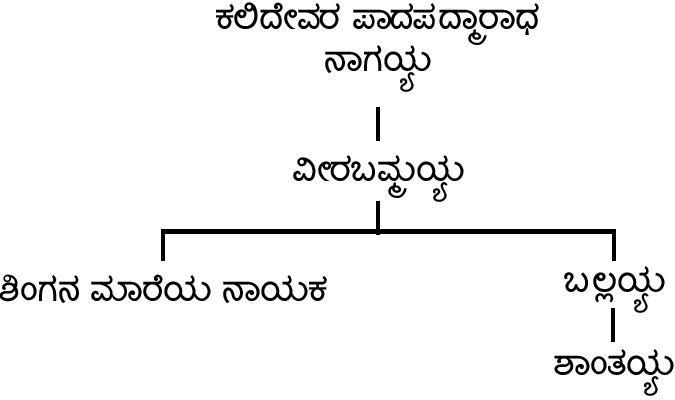
\includegraphics[scale=1.1]{images/chap4/chap4fig7.jpeg}
\end{figure}

\newpage

ವೀರಬಲ್ಲಾಳನು ದೋರಸಮುದ್ರದಿಂದ ಆಳುತ್ತಿದ್ದಾಗ, ಅವನ ಮಹಾ ಸಾಮಂತ “ಕಲಿದೇವರ ಪಾದಪದ್ಮಾರಾಧಕ ನಾಗಯ್ಯ ಮತ್ತು ಭಕ್ತರ ಕರುಣದ ಕಾರಣ್ಯದ ಮಗ, ಶರಣರ ದಾಸ ಶೋವನ (ಶೋಭನ), ವೀರ ಬಮ್ಮಯ್ಯನ ಮಗ, ಶಿಂಗನ ಮಾರೆಯ ನಾಯಕ ಇವರುಗಳು ಯೆಮ್ಮೆಯಕೇತನ ಹಟ್ಟಿಯನ್ನು ಶ‍್ರೀ ಕಲಿದೇವರಿಗೆ ಶಿವಪುರಿಯಾಗಿ ಭಕ್ತರಿಗೆ ಧರ್ಮವಾಗಿ” ಕೊಟ್ಟರೆಂದು ಮಂಡಿಪುರ ಶಾಸನದಲ್ಲಿ ಹೇಳಿದ್ದು, ಈ ಶಾಸನ ವೀರಶೈವಧರ್ಮದ ಪರಿಭಾಷೆಯಿಂದ ಕೂಡಿದೆ.

ಈ ಶಿವಪುರವನ್ನು "ಅಟಕೇಶ್ವರ ದೇವರ ತೊತ್ತು ವೀರಬಮ್ಮಯ್ಯ\index{ವೀರಬಮ್ಮಯ್ಯ}, ಚೂಡಮದೇವರ ಅಂಕಯ್ಯ\index{ಚೂಡಮದೇವರ ಅಂಕಯ್ಯ}, ಮಲ್ಲಿನಾಥದೇವರ ಜಕ್ಕಯ್ಯ\index{ಮಲ್ಲಿನಾಥದೇವರ ಜಕ್ಕಯ್ಯ}, ಸೋಮನಾಥದೇವರ ಕೇತಯ್ಯ ಅಪ್ಪಯ್ಯ\index{ಸೋಮನಾಥದೇವರ ಕೇತಯ್ಯ ಅಪ್ಪಯ್ಯ}, ಮಲ್ಲಿನಾಥ ದೇವರ ಯೇಚಯ್ಯ\index{ಮಲ್ಲಿನಾಥ ದೇವರ ಯೇಚಯ್ಯ}, ರಾಮನಾಥದೇವರ ಹೊಯಿಶಣದಾಶಿ\index{ರಾಮನಾಥದೇವರ ಹೊಯಿಶಣದಾಶಿ}, ಚೂಡಮದೇವರ ಮಾಚಯ್ಯ\index{ಚೂಡಮದೇವರ ಮಾಚಯ್ಯ}, ಅಂಕನಾಥದೇವರ ಹೊಂನಯ್ಯ, ಚೂಡಮದೇವರ ಲೆಂಕ ಬೂವಣ್ನ ಯಿಂತನಿಬರಿಗೂ ಧಾರಾಪೂರ್ವಕ" ಮಾಡಿಕೊಡಲಾಗಿದೆ. ಶಿವಪುರವನ್ನಾಗಿ ದತ್ತಿ ಪಡೆದ ಭಕ್ತರ ಜೊತೆ ಅವರ ದೇವರುಗಳ ಹೆಸರುಗಳೂ ಬಂದಿರುವುದನ್ನು ವಿಶೇಷವಾಗಿ ಗಮನಿಸಬೇಕು. ಇದು ಅವರ ಇಷ್ಟಲಿಂಗಗಳ\index{ಇಷ್ಟಲಿಂಗಗಳು} ಹೆಸರುಗಳಾಗಿವೆ. ವಚನಕಾರರೂ ಈ ರೀತಿ ತಮ್ಮ ಇಷ್ಟದೈವ/ಲಿಂಗದ ಹೆಸರನ್ನು ಅಂಕಿತವಾಗಿ ಮಾಡಿಕೊಂಡಿದ್ದಾರೆ. ಮೇಲ್ಕಂಡ ವೃತ್ತಿವಂತರು ವಚನಕಾರರಾಗಿದ್ದ ಪಕ್ಷದಲ್ಲಿ,\break ದೇವರ ಹೆಸರು ಅವರ ಅಂಕಿತಗಳಾಗಿರಬಹುದೆಂದು ಊಹಿಸಬಹುದು.

ಚೂಡಮ ದೇವರ ಲೆಂಕ ಬೂವಣ್ನ ಎಂಬಲ್ಲಿ ಲೆಂಕ\index{ಲೆಂಕ} ಎಂಬ ಪದ ಬಹಳ ಮುಖ್ಯವಾಗುತ್ತದೆ. ವೀರಶೈವರು ಅಥವಾ ಶಿವಭಕ್ತರು ನರರಾದ ರಾಜಮಹಾರಾಜರ ಲೆಂಕರಾಗದೆ ಶಿವನಿಗೆ ಲೆಂಕರಾಗಿರುತ್ತಿದ್ದರು. ಶಿವಲೆಂಕ ಮಂಚಣ್ಣ (ಕ್ರಿ.ಶ. 1160) ಎಂಬ ಶರಣನ ಹೆಸರನ್ನು ಇದು ನೆನಪಿಗೆ ತರುತ್ತದೆ.\endnote{ ಕನ್ನಡ ಅಧ್ಯಯನ ಸಂಸ್ಥೆಯ ಕನ್ನಡ ಸಾಹಿತ್ಯ ಚರಿತ್ರೆ, ಸಂಪುಟ 4, ಶಿವಲೆಂಕ ಮಂಚಣ್ಣ - ಬಿ.ಎಸ್​. ಸಣ್ಣಯ್ಯ, ಪುಟ766-769} ಕೊಂಡಗುಳಿ ಕೇಶಿರಾಜ, ತೆಲುಗು ಜೊಮ್ಮಣ್ಣ, ಶಂಕರ ದಾಸಿಮಯ್ಯ, ಇವರು ಉಗ್ರಭಕ್ತರು. ಹರಿಹರನು ತೆಲುಗು ಜೊಮ್ಮಯ್ಯಗಳ ರಗಳೆಯಲ್ಲಿ \textbf{"ಜೋಳವಾಳಿಯೊಳಿರ್ಪನಾ\index{ಜೋಳವಾಳಿ} ಧರಾನಾಥಂಗೆ, ವೇಳೆವಾಳಿಯೊಳಿರ್ಪನಾ\index{ವೇಳೆವಾಳಿ} ಭೀಮನಾಥಂಗೆ,"} ಎಂದು ಹೇಳಿದ್ದಾನೆ. ಅದೇರೀತಿ ಶಂಕರ ದಾಸಿಮಯ್ಯನ ರಗಳೆಯಲ್ಲಿ \textbf{"ಎಲೆ ದೇವಾ ಚಂದ್ರಧರಾ ಸಕಲ ಸಸ್ಯಾಧಿಪತಿಯೇ, ಜೋಳದ ಪೆಸರುಂ ನಿನ್ನ ಪೆಸರಾಗಿರ್ದಪುದು, ಎನಗರಿದೆಂದು ವೇಳೆವಾಳಿಯವಂ, ಜೋಳವಾಳಿಯವನಲ್ಲಲ್ಲ"} ಎಂದೂ ಹೇಳಿದ್ದಾನೆ. ಶಿವಲೆಂಕ ಮಂಚಣ್ಣ ಮತ್ತು ಶಂಕರ ದಾಸಿಮಯ್ಯ ಇಬ್ಬರೂ ಶಿವೇತರ ದೈವಗಳ ಪ್ರತಿಮೆಗಳನ್ನು ನಾಶಮಾಡಿದವರೆಂಬುದು ಗಮನಿಸಬೇಕಾದ ಸಂಗತಿ.

ಮರಡಿಪುರ ಶಾಸನದಲ್ಲಿ ಶಿವ ಮತ್ತು ಕಲಿದೇವ ಒಬ್ಬನೇ ಎಂದು ಹೇಳುವುದಲ್ಲದೆ, ನಂದಿನಾಥ, ಭೃಂಗಿನಾಥ, ವೀರಭದ್ರ, ಮಹಾಕಾಲ ಮೊದಲಾದ ಗಣಂಗಳಿಂದ ಶಿವನು ಸೇವಿತನಾಗಿದ್ದನೆಂದು ಹೇಳಿದೆ.\endnote{ ನೇಗಿನಹಾಳ್​, ಡಾ. ಎಂ.ಬಿ., ನೇಗಿನಹಾಳ ಪ್ರಬಂಧಗಳು, ಶಾಸನಗಳಲ್ಲಿ ವೀರಭದ್ರ ದೇವರು, ಪುಟ 383}

ಇದಿಷ್ಟೂ ಮಂಡ್ಯ ಜಿಲ್ಲೆಯ ವೀರಶೈವ ಶಾಸನಗಳಲ್ಲಿ ಒಂದು ಘಟ್ಟ. ಕಲ್ಯಾಣದ ಕ್ರಾಂತಿಯ ನಂತರ ಇತರ ಧರ್ಮಗಳಂತೆ, ವೀರಶೈವಧರ್ಮಕ್ಕೂ ಅದರ ಪ್ರಸಾರಕರಾದ ಶಿವಶರಣರು ಮತ್ತು ಶಿವಭಕ್ತರಿಗೂ ಇನ್ನೊಂದು ಘೋರ ವಿಪತ್ತು 13ನೇ ಶತಮಾನದ ಅಂತ್ಯದಲ್ಲಿ ಸಂಭವಿಸಿತು. ಉತ್ತರ ದಿಕ್ಕಿನಿಂದ 1294 ರ ಹೊತ್ತಿಗೆ ಸೇವುಣ ರಾಜ್ಯದ ಮೇಲೆ ಮಹಮದೀಯರ ದಾಳಿ ಆರಂಭವಾಯಿತು. ಅದು ಮುಂದುವರಿದು 1318ರ ಹೊತ್ತಿಗೆ ದೇವಗಿರಿ, 1323ರ ಹೊತ್ತಿಗೆ ಓರುಗಲ್ಲು, 1327ರ ಹೊತ್ತಿಗೆ ಕಮ್ಮಟದುರ್ಗಗಳು ಮಹಮದೀಯರ ವಶವಾದವು. ಮಹಮದೀಯರ ನೇರ ದಾಳಿಗೆ ಸಿಗದೆ ಉಳಿದುಕೊಂಡಿದ್ದು ಮುಮ್ಮಡಿ ಬಲ್ಲಾಳನು\index{ಮುಮ್ಮಡಿ ಬಲ್ಲಾಳನು} ಆಳುತ್ತಿದ್ದ ಹೊಯ್ಸಳರ ರಾಜ್ಯ ಒಂದೇ. ಶಿವಶರಣರು ವೈಯಕ್ತಿಕ ರಕ್ಷಣೆ, ಧರ್ಮರಕ್ಷಣೆ ಮತ್ತು ಧರ್ಮ ಪ್ರಸಾರದ ದೃಷ್ಟಿಯಿಂದ ಹೊಯ್ಸಳ ರಾಜ್ಯದ ಕಡೆಗೆ ಬರತೊಡಗಿದರು. ಈ ದೃಷ್ಟಿಯಿಂದ ಕೃಷ್ಣರಾಜಪೇಟೆ ತಾಲ್ಲೂಕಿನ ಹೊಸಹೊಳಲಿನ\index{ಹೊಸಹೊಳಲು} ಶಾಸನ ಪ್ರಮುಖವಾಗುತ್ತದೆ.\endnote{ ಎಕ 6 ಕೃಪೇ 8 ಹೊಸಹೊಳಲು 1306}

\textbf{ಹೊಸಹೊಳಲು ಶಾಸನದ ಸಪ್ಪೆಯ ಕೇತಯ್ಯ\index{ಸಪ್ಪೆಯ ಕೇತಯ್ಯ} ಮತ್ತು ಹುಲಿಗೆರೆ ದೇವರು ಸೋಮಯ್ಯ\index{ಹುಲಿಗೆರೆ ದೇವರು ಸೋಮಯ್ಯ}:} ಹೊಸ ಹೊಳಲು ಶಾಸನವು \textbf{ಸ್ವಸ್ತಿ ಸಮಸ್ತ ಪ್ರಸಸ್ತಿ ಸಹಿತಂ ನಂದಿನಾಥ ವೀರಭದ್ರದೇವರು ಮುಖ್ಯವಾದ ಪ್ರಿಥುವಿಯ ಮಹಾಗಣಂಗಳು}" ಎಂದು ಮುಂದುವರಿಯುತ್ತದೆ. ಈ ಮಹಾಗಣಗಳು \textbf{"ಹೊಇಸಣ ನಾಡು\index{ಹೊಇಸಣ ನಾಡು}, ಕೊಂಗನಾಡು\index{ಕೊಂಗನಾಡು} ಮುಖ್ಯವಾದ ಹದಿನೆಂಟು ಸೀಮೆಯೊಳಗೆ\index{ಹದಿನೆಂಟು ಸೀಮೆ} ಹೊಸಒಳಲ ಬಡಗಣ ಹೆಬಾಗಿಲ ಆಲದಮರದೆಲೆ ಸಿಂಹಾಸನದ ಮೇಲೆ ವಜ್ರದ ಬಇಸಣಿಗೆಯನಿಕ್ಕಿ ಮಾಡಿದಡೀ"} ಎಂಬುದು ಶಾಸನದ ಮುಖ್ಯಪಾಠ. (ಶಿವನ) ಮಹಾಗಣಂಗಳು ಅಂದರೆ ಶರಣರ ಸಮೂಹ ಬೇರೆಕಡೆಯಿಂದ ಬಹುಶಃ ಪು(ಹು)ಲಿಗೆರೆಯ ಕಡೆಯಿಂದ ಬಂದು, ಅನಾದಿ ಅಗ್ರಹಾರವೂ, ಹೊಯ್ಸಳರ ಕಾಲದ ಪ್ರಮುಖ ಪಟ್ಟಣವೂ ಆಗಿದ್ದ ಹೊಸಹೊಳಲ ಬಡಗಣ (ಉತ್ತರ ದಿಕ್ಕು) ಹೆಬ್ಬಾಗಿಲಿನಲ್ಲಿ ಆಲದ ಮರದ ಕೆಳಗೆ ವಜ್ರಾಸನದಲ್ಲಿ ಕುಳಿತರು ಎಂದು ಈ ಶಾಸನಪಾಠವನ್ನು ಅರ್ಥೈಸಬಹುದು. ಈ ಶಾಸನ ಹಾಗೂ ಸೋಮನಾಥ ದೇವಾಲಯದ ಬಳಿ ಈಗಲೂ ಕೂಡಾ ಹೆಬ್ಬಾಗಿಲು ಹಾಗೇ ಉಳಿದಿದೆ. ಈ ರೀತಿ ಬಂದ ಅಸಂಖ್ಯಾತ ಗಣಂಗಳ ಮುಖ್ಯಸ್ಥರಾಗಿ \textbf{"ಸಪ್ಪೆಯ ಕೇತಯ್ಯಂಗಳ ಮಕ್ಕಳಾ ಹುಲಿಗೆರೆ ದೇವರು ಸೋಮಯ್ಯಂಗಳು"} ಇದ್ದರು. ಆದುದರಿಂದ ಇವರ ಹೆಸರನ್ನು ಮಾತ್ರ ಶಾಸನದಲ್ಲಿ ಉಲ್ಲೇಖಿಸಲಾಗಿದೆ ಎಂದು ಹೇಳಬಹುದು.

ಸಪ್ಪೆಯ ಕೇತಯ್ಯನ ಹೆಸರು ವೀರಶೈವ ಸಾಹಿತ್ಯದಲ್ಲಿ ಎಲ್ಲಿಯೂ ಕಂಡು ಬರುವುದಿಲ್ಲ. ಸೊಪ್ಪೆಯ ಬಸವಣಯ್ಯ\index{ಸೊಪ್ಪೆಯ ಬಸವಣಯ್ಯ} ಅಥವಾ ಶಿದ್ಧಬಸವನ ಚರಿತ್ರೆಯು, ಲಕ್ಕಣ್ಣ ದಂಡೇಶನ ಶಿವತತ್ವ ಚಿಂತಾಮಣಿ, ವಿರೂಪಾಕ್ಷ ಪಂಡಿತನ ಚನ್ನಬಸವ ಪುರಾಣ, ಸಿದ್ಧನಂಜೇಶನ ಗುರುರಾಜ ಚಾರಿತ್ರ್ಯ ಇವುಗಳಲ್ಲಿ ವರ್ಣಿತವಾಗಿದೆ. ಕಂಚಿಯಲ್ಲಿ ಜನಿಸಿದ ಈತನು ಬಹುಮನಿ ಸುಲ್ತಾನ ಫಿರೋಜ್​ ಶಹಾನ ಕಾಲದಲ್ಲಿ (1397-1422) ಕಲಬುರ್ಗಿ ಜಿಲ್ಲೆ, ಜೇವರಗಿ ತಾಲ್ಲೂಕಿನ ಕೊಳಕೂರಿನಲ್ಲಿದ್ದು ಪವಾಡವನ್ನು ಮೆರೆದು ಅಲ್ಲೇ ಐಕ್ಯನಾದನು. ಇನ್ನೊಬ್ಬ ಸೊಪ್ಪೆಯ ಲಿಂಗಣಾರ್ಯನೆಂಬುವವನು\index{ಸೊಪ್ಪೆಯ ಲಿಂಗಣಾರ್ಯ} ಮಳಲವಾಡಿಯಲ್ಲಿದ್ದು ಪವಾಡವನ್ನು ಮೆರೆದವನು. ಗುಬ್ಬಿಯ ಮಲ್ಲಣಾರ್ಯನ ವೀರಶೈವಾಮೃತ ಮಹಾಪುರಾಣದಲ್ಲಿ ಇವನ ಕಥೆ ಬರುತ್ತದೆ.\endnote{ ಶಿವಶರಣ ಕಥಾರತ್ನ ಕೋಶ, ತ.ಸು. ಶಾಮರಾವ್​,} ತೋಂಟದ ಸಿದ್ಧಲಿಂಗ ಯತಿಗಳ ಶಿಷ್ಯ ಪರಂಪರೆಯಲ್ಲಿ ಸಪ್ಪೆಯ ದೇವನೆಂಬುವವನಿದ್ದಾನೆ.\endnote{ \engfoot{EC XI (B.L.Rice)} ಕುಣಿಗಲ್​ 49 ಯೆಡಿಯೂರು} ಈ ಶಾಸನದ ಕಾಲ ಶಾಸನದ ಕಾಲ 1606 ರ ನಂತರ ಎಂದು ಡಾ.ಎಲ್​. ಬಸವರಾಜು ಅವರು ಹೇಳುತ್ತಾರೆ.\endnote{ ವಚನಕಾರ ಸಿದ್ಧಲಿಂಗ ಯತಿ (ಬೆಂಗಳೂರು ವಿ.ವಿ.) ಪುಟ19 ಮತ್ತು 26} 12ನೇ ಶತಮಾನದಲ್ಲಿ ಶಿವಶರಣರು ಆಗಿಹೋದಮೇಲೆ ಮತಪ್ರಚಾರಕ್ಕಾಗಿ ನಾಡಿನ ನಾನಾ ಕಡೆಗಳಲ್ಲಿ ಅನೇಕ ಮಠಗಳು ಸ್ಥಾಪಿತವಾದವು. ಅವುಗಳಲ್ಲಿ ಸೊಪ್ಪೆಯ ಮಠವೂ ಒಂದು. ಸೊಪ್ಪೆಯ ಶಾಖಾ ಮಠಗಳು ಆಂಧ್ರ, ತಮಿಳುನಾಡು, ಕರ್ನಾಟಕದಲ್ಲಿವೆ. ಕರ್ನಾಟಕದ ಬಳಗಾನೂರು, ಸಿಂಧಗಿ, ವಿಜಾಪುರ, ಮದ್ರವಾಡ, ಪ್ಯಾರಸಾಬಾದ್​ ( ಇದು ಕೊಳಕೂರಿನ ಸಮೀಪ ಇದೆ), ಯರಗಲ್​, ಇಳಕಲ್​, ಹರವಾಳಗಳಲ್ಲಿವೆ. ಈ ಮಠದ ಸ್ವಾಮಿಗಳನ್ನು ಸೊಪ್ಪೆಯ ದೇವರು\index{ಸೊಪ್ಪೆಯ ದೇವರು}, ಸೊಪ್ಪೆಯಾರ್ಯ\index{ಸೊಪ್ಪೆಯಾರ್ಯ} ಎಂದು ಕರೆಯುವುದು ರೂಢಿ. ತೋಂಟದ ಸಿದ್ಧಲಿಂಗ ಯತಿಗಳ ಕಾಲಕ್ಕೆ ಮುಂಚೆ ಇವರು ಕರ್ನಾಟಕದಲ್ಲಿ ಸಂಚರಿಸಿ ತಮ್ಮ ಸಂದೇಶ ಬೀರಿದರು.\endnote{ ಸಗರನಾಡಿನ ಶಿವರಶರಣರು, (ಕರ್ನಾಟಕ ವಿವಿ), ಡಾ.ವಿ.ಶಿವಾನಂದ್​, ಪುಟ 37-40} ಆದುದರಿಂದ ಹೊಸಹೊಳಲು ಶಾಸನೋಕ್ತ ಸಪ್ಪೆಯ ಕೇತಯ್ಯ, ಈ ಸಪ್ಪೆ ಮಠದ ಪರಂಪರೆಯ ಪ್ರಾಚೀನ ಯತಿಗಳಲ್ಲಿ ಒಬ್ಬನಿರಬಹುದೆಂದು ಹೇಳಬಹುದು

\textbf{"ಸಪ್ಪೆಯ ಕೇತಯ್ಯಂಗಳ ಮಕ್ಕಳಾ ಪುಲಿಗೆರೆ ದೇವರು ಸೋಮಯ್ಯಂಗಳು"} ಎಂದಿರುವುದರಿಂದ ಈತ ಸಪ್ಪೆಯ ಕೇತಯ್ಯನ ಮಗ ಅಥವಾ ಶಿಷ್ಯ ಎಂದಾಗುತ್ತದೆ. ತನ್ನ ಭಕ್ತಿ ಹಾಗೂ ವೀರವ್ರತದಿಂದ ಪುಲಿಗೆರೆಯ ಸುರಹೊನ್ನೆ ಬಸದಿಯಲ್ಲಿದ್ದ ಜಿನಬಿಂಬವು ಒಡೆದು ಅಲ್ಲಿ ಶಿವಲಿಂಗವು ಒಡಮೂಡುವಂತೆ ಮಾಡಿದ ಪವಾಡವನ್ನು ಎಸಗಿದ ಪುಲಿಗೆರೆ ಸೋಮಯ್ಯನ\index{ಪುಲಿಗೆರೆ ಸೋಮಯ್ಯ} ಕಥೆ ಅನೇಕ ವೀರಶೈವ ಕಾವ್ಯಗಳು ಪುರಾಣಗಳಲ್ಲಿ ಬಂದಿದೆ.\endnote{ ಶಿವಶರಣ ಕಥಾರತ್ನಕೋಶ, ತ.ಸು.ಶಾಮರಾವ್​, ಪುಟ 252} ಪುಲಿಗೆರೆಯ ಸೋಮೇಶ್ವರ ದೇವರಿಗೆ ಸಂಬಂಧಿಸಿದಂತೆ, ಸೋಮಯ್ಯ ಮತ್ತು ಆದಯ್ಯ ಇಬ್ಬರ ಹೆಸರು ತಳುಕು ಹಾಕಿಕೊಂಡಿದ್ದು, ಈ ಕಥಾಪರಂಪರೆಯ ಬಗ್ಗೆ ಡಾ.ಎಂ.ಎಂ. ಕಲಬುರ್ಗಿಯವರು ವಿಸ್ತಾರವಾಗಿ ವಿವೇಚಿಸಿದ್ದಾರೆ.\endnote{ ಪುಲಿಗೆರೆಯ ಸೋಮೇಶ್ವರ, ಪುಟ 324-36, ಮಾರ್ಗ-ಸಂಪುಟ 1, ಎಂ.ಎಂ. ಕಲಬುರ್ಗಿ} ಪುಲಿಗೆರೆಯ ವೀರಶೈವಪೀಠ ಪರಂಪರೆಯ ಬಗ್ಗೆಯೂ ಕೂಡಾ, ಎಂ.ಎಂ. ಕಲಬುರ್ಗಿಯವರು ವಿವೇಚಿಸದ್ದಾರೆ.\endnote{ ಪುಲಿಗೆರೆಯ ಒಂದು ವೀರಶೈವಪೀಠ ಪರಂಪರೆ, ಪುಟ 144-48, ಮಾರ್ಗ-ಸಂಪುಟ 2, ಎಂ.ಎಂ.ಕಲಬುರ್ಗಿ} ಈ ಕಾಲದಲ್ಲಿ ಪುಲಿಗೆರೆಯ\index{ಪುಲಿಗೆರೆ} ಕಡೆಯಿಂದ ಈ ಭಾಗಕ್ಕೆ ಬಂದು ಸೋಮನಾಥನನ್ನು ಪ್ರತಿಷ್ಠಾಪಿಸುವ ಅಥಾವ ಶೈವ ದೇವಾಲಯಗಳಲ್ಲಿ, ಶೈವಕ್ಷೇತ್ರಗಳಲ್ಲಿ ನೆಲೆಸುವ ವೀರಶೈವ ಭಕ್ತರ ಒಂದು ಪರಂಪರೆ ಇತ್ತು ಎಂಬುದಕ್ಕೆ ಈ ಭಾಗದ ಇತರ ಶಾಸನಗಳಿಂದಲೂ ಸೂಚನೆಗಳು ಸಿಗುತ್ತವೆ. ಬಳ್ಳಾರಿ ಜಿಲ್ಲೆ, ಹಡಗಲಿ ತಾಲ್ಲೂಕು, ಕುರುವತ್ತಿಯ ಮಲ್ಲಿಕಾರ್ಜುನ ದೇವಾಲಯದಲ್ಲಿರುವ ಯಾದವ ಸಿಂಘಣನ ಕಾಲದ ಶಾಸನದಲ್ಲಿ, ಹುಲಿಗೆರೆಯ ಸೋಮನಾಥ ದೇವರ ಪುತ್ರಿಕಂ ಗಣಕುಮಾರರಾದ ಸತ್ತಿದೇವರು ಮುಖ್ಯವಾಗಿ ಹನ್ನೆರಡು ಮಾಹೇಶ್ವರರಿಗೆ (ಶಿವಭಕ್ತರಿಗೆ-ಶರಣರಿಗೆ), ದೇವಪುರದೊಳಗೆ ಹನ್ನೆರಡು ಮನೆಯನ್ನು ರಾಜಗುರು ಸೂರ್ಯಾಭರಣ ಪಂಡಿತರ ಸಮ್ಮುಖದಲ್ಲಿ ದತ್ತಿ ಬಿಡಲಾಗಿದೆ.\endnote{ ಕನ್ನಡ ವಿ.ವಿ. ಶಾಸನಸಂಪುಟ, ಬಳ್ಳಾರಿ ಜಿಲ್ಲೆ, ಹಡಗಲಿ 9 ಕುರುವತ್ತಿ 1225} ಬೇಲೂರು ತಾಲ್ಲೂಕಿನ ಸಿದ್ಧಾಪುರ ಶಾಸನದಲ್ಲಿ, ಹುಲಿಗೆರೆಯ ಸೋಮನಾಥ\index{ಹುಲಿಗೆರೆಯ ಸೋಮನಾಥ} ದೇವರ ಕ್ಷೇತ್ರವಾಸಿಗಳಪ್ಪ ಪುರಾಣದ ಮಾಯಿದೇವ ಪಂಡಿತರ ಶ‍್ರೀಪಾದದ ಕಾರುಂಣ್ಯದ ಸಿಸು, ಸಕಳ ನೇಮಸಂಪನ್ನರುಮಪ್ಪ ಶ‍್ರೀ ಶಿವರಾತ್ರಿಯ ಮಾಯಿದೇವರಿಗೆ ದತ್ತಿ ಬಿಡಲಾಗಿದೆ.\endnote{ ಎಕ 9 ಬೇಲೂರು 439 ಸಿದ್ಧಾಪುರ 1285} ಮರಡಿಪುರ ಶಾಸನದಲ್ಲೂ ಕೂಡಾ ಸೋಮನಾಥ ದೇವರ ಕೇತಯ್ಯ ಎಂಬ ಶರಣನ ಹೆಸರು ಉಲ್ಲೇಖಿತವಾಗಿದೆ. ಈತ ಪುಲಿಗೆರೆಯಿಂದ ಬಂದವನಿರಬಹುದು. ಕ್ರಿ.ಶ. 1510ರ ಮಳವಳ್ಳಿ ತಾಲ್ಲೂಕಿನ\break ನಡಗಲ್​ಪುರ ಶಾಸನದಲ್ಲಿ, ದಕ್ಷಿಣ ಸೋಮೇಶ್ವರ ದೇವರ ದೇವದಾನ" ಬಿಟ್ಟರೆಂದು ಹೇಳಿದೆ.\endnote{ ಎಕ 7 ಮವ 44 ನಡಗಲ್​ಪುರ 1510} ಈ ರೀತಿಯಾಗಿ ಪುಲಿಗೆರೆಯಿಂದ ಈ ಕಡೆಗೆ ಶಿವಶರಣರು ಬರುತ್ತಿದ್ದರೆಂಬುದು, ಅಂತಹ ಶಿವಶರಣರಲ್ಲಿ ಸಪ್ಪೆಯ ಕೇತಯ್ಯಂಗಳ ಮಕ್ಕಳಾ ಹುಲಿಗೆರೆ ದೇವರು ಸೋಮಯ್ಯಂಗಳು ಒಬ್ಬರಿರಬಹುದು. ಪುಲಿಗೆರೆಯ ಸೋಮೇಶ್ವರ ದೇವರು ಈ ಭಾಗದಲ್ಲಿ ಪ್ರಸಿದ್ಧಿಯನ್ನು ಪಡೆದಿತ್ತೆಂಬುದು ಹೇಳಬಹುದು.

ಈ ಕಾಲದ ಹಾಗೂ ನಂತರದ ವೀರಶೈವ ಶಾಸನಗಳು, ವೀರಶೈವ ಗೋತ್ರ/ಗಣಗಳ ಉಲ್ಲೇಖದೊಡನೆ, \textbf{ಸ್ವಸ್ತಿ ಸಮಸ್ತ ಪ್ರಸಸ್ತಿ ಸಹಿತಂ ನಂದಿನಾಥ\index{ನಂದಿನಾಥ} ವೀರಭದ್ರದೇವರು ಮುಖ್ಯವಾದ ಪ್ರಿಥುವಿಯ ಮಹಾಗಣಂಗಳು\index{ಪ್ರಿಥುವಿಯ ಮಹಾಗಣಂಗಳು}"} ಎಂದು ಆರಂಭವಾಗುತವೆ. ಅಗರ ಶಾಸನವು,\endnote{ ಎಕ 4 ಯಳಂದೂರು 140 ಅಗರ - 15ನೇ ಶತಮಾನ}\textbf{“ಸ್ವಸ್ತಿ ಸಮಸ್ತ ಪ್ರಶಸ್ತಿ ಸಹಿತಂ ಶ‍್ರೀ ನಂದಿನಾಥ ಭ್ರುಂಗಿನಾಥ\index{ಭ್ರುಂಗಿನಾಥ} ವೀರಭದ್ರ ದೇವರು\index{ವೀರಭದ್ರ ದೇವರು} ಮುಖ್ಯವಾದ ಸಜನ ಸುದ”} ಎಂದು ಆರಂಭವಾಗುತ್ತದೆ. ಕುಂತೂರು ಶಾಸನವು \textbf{“ಸ್ವಸ್ತಿ ಸಮಸ್ತ ಪ್ರಸಸ್ತಿ ಸಹಿತ ಶ‍್ರೀ ನಂದಿನಾಥ ಭ್ರುಂಗಿನಾಥ, ವೀರಭದ್ರ ದೇವರು ಮುಖ್ಯವಾದ ಸಜ್ಜನ ಶುದ್ಧ ಶಿವಾಚಾರ\index{ಶಿವಾಚಾರ} ಸಂಪನ್ನರುಮಪ್ಪ ದೇವಾಪ್ರುಥುವೀ ಮಹಾಮಹತ್ತಿನೊಳಗಾದ\index{ಮಹಾಮಹತ್ತಿ} ಸಾಲೂರ ಶಾಂತದೇವರು\index{ಸಾಲೂರ ಶಾಂತದೇವರು}”} ಎಂದು ಆರಂಭವಾಗುತ್ತದೆ. ಸುಪ್ರಸಿದ್ಧವಾದ ಕೆಂಪನಪುರ\index{ಕೆಂಪನಪುರ} ಶಾಸನವು\endnote{ ಎಕ 4ಚಾಮರಾಜನಗರ 144 ಕೆಂಪನಪುರ 15ನೇ ಶತಮಾನ}\textbf{ "ಶ‍್ರೀಮದ್ವೀರ ಸೋಮೇಶ್ವರ ದ್ವಾದಶಾವತಾರ ಶ‍್ರೀ ವೀರಭದ್ರ ನಿಜಸ್ವರೂಪ ಶ‍್ರೀಮದೇಕಾಂತ ರಾಮೇಶ್ವರಾನ್ವಯೋದ್ಭೂತ ಸಕಲಶಾಸ್ತ್ರ ಪಾರಾವಾರ ಪಾರಂಗತ ವೀರಶೈವ ಮತ\index{ವೀರಶೈವ ಮತ} ಸ್ಥಾಪನಾಚಾರ್ಯ"} ಎಂಬುದಾಗಿ ಪ್ರಾರಂಭವಾಗುತ್ತದೆ. \textbf{ಶಾಸನಗಳಲ್ಲಿ ಬಹಳ ಅಪರೂಪವಾಗಿ ಪ್ರಯೋಗವಾಗಿರುವ ವೀರಶೈವ ಪದ ಪ್ರಯೋಗವನ್ನು ಇಲ್ಲಿ ಗಮನಿಸಬಹುದು.} ಬಹು ದೂರದ ಆಂಧ್ರ ಪ್ರದೇಶದ ಆಲಂಪುರದಲ್ಲಿರುವ ಶಾಸನವೂ\endnote{ ಆಂಧ್ರಪ್ರದೇಶದ ಕನ್ನಡ ಶಾಸನಗಳು, ಭಾಗ-2, ಮಹಬೂಬ್​ನಗರ ಜಿಲ್ಲೆ, ಆಲಂಪುರ ತಾಲ್ಲೂಕು 492 ಆಲಂಪುರ 1593} ಕೂಡಾ \textbf{"ಶ‍್ರೀಮತ್ಪರಮ ವೀರಶೈವ ಶಿಧಾಂತ ಸಂನ್ಮಾರ್ಗ್ಗ ಸಂಪ್ಪಂನ್ನ ಸದ್ವೀರ ಮಾಹೇಶ್ವರ ಹೃತ್ಕಮಲ ಕಂರ್ಣ್ನಿಕಾ ನಿವಾಸ ಚಿಂನ್ಮೂರ್ತ್ತಿ ಪ್ರಾಣಲಿಂಗ ಸಮಾರ್ಚನಾಮ ಸಂತ್ತಿಷ್ಟ ರುಗ್ವೇದ ಶಾಸ್ತ್ರಾಗಮ ಪುರಾಣ ಯಿತಿಹಾಸಾದಿ ನಾನಾ ಶಾಸ್ತ್ರ ಕೋವಿದುರುಂ ಜೈನ\index{ಜೈನ} ಚಾರ್ವಾಕ\index{ಚಾರ್ವಾಕ} ಮಾಯಾವಾದ\index{ಮಾಯಾವಾ} ಮೊದಲಾದ ಪರವಾದಿ ಕೋಲಾಹಲರುಂ ಗುರುಲಿಂಗ್ಗ ಜಂಗ್ಗಮ ಪಾದೋದಕ ಪ್ರಸಾದಾನುಭಾವಿಗಳಪ್ಪ\index{ಗುರುಲಿಂಗ್ಗ ಜಂಗ್ಗಮ ಪಾದೋದಕ ಪ್ರಸಾದ} ಶ‍್ರೀ ನಂದ್ದಿನಾಥ ಭೃಂಗ್ಗಿನಾಥ ಶ‍್ರೀ ವೀರಭದ್ರ ದೇವರು ಮುಖ್ಯವಾದ ಅಸಂಖ್ಯಾತ ಮಹಾಗಣಂಗ್ಗಳು ಸಭಾ ಮಧ್ಯದಲ್ಲಿ ಮಣಿಗಣಖಚಿತ ಶಿಂಹಾಸ್ವನಾರೂಢರಾದ ಪೃಥಿವೀಗೆ ಭೂಕಯಿಲಾಸವೆನಿಸುವ ಶ‍್ರೀಗಿರಿ ಶಿಂಹಾಸ್ವನದ ಮಹಾಮಹಾತ್ಮರಾದ"} ಈ ರೀತಿಯಾಗಿ ವೀರಶೈವಧರ್ಮದ ಪ್ರಸಾರದಲ್ಲಿ ವೀರಭದ್ರ, ನಂದೀನಾಥ, ಭೃಂಗೀನಾಥ, ಸೋಮೇಶ್ವರ ಈ ವೀರಪರಂಪರೆಯ ದೇವರುಗಳಿಗೆ ಪ್ರಾಧಾನ್ಯ ನೀಡಿರುವುದು ಇದರಿಂದ ತಿಳಿದುಬರುತ್ತದೆ. ವೀರಶೈವ ಶಾಸನಗಳನ್ನು ಗುರುತಿಸಲು ಈ ದೇವರುಗಳ (ಗೋತ್ರ) ಉಲ್ಲೇಖ ಪ್ರಮುಖವಾಗುತ್ತದೆಂದು ಹೇಳಬಹುದು. “ನಂದಿ, ಭೃಂಗಿ, ವೀರಭದ್ರ ದೇವರಿಗೆ ಪ್ರಾಶಸ್ತ್ಯವುಳ್ಳ, ದ್ಯಾವಾ ಪೃಥ್ವಿ, ಮಹಾಮಹತ್ತಿನ ಸಂಪ್ರದಾಯ ಒಂದಾದರೆ, ಅನೇಕಾಂತ ವಿರೋಧಿ, ಏಕಾಂತವಾದಿಯಾದ ಇನ್ನೊಂದು ಪರಂಪರೆ 15ನೇ ಶತಮಾನದವರೆಗೆ ಕೆಲಮಟ್ಟಿಗೆ ಪ್ರತ್ಯೇಕ ಅಸ್ತಿತ್ವವನ್ನು ಉಳಿಸಿಕೊಂಡು ಬಂದಿತೆಂದೂ, ಅದೂ ಕೂಡಾ ವೀರಭದ್ರ ದೇವರ ಪೂಜೆಯನ್ನು ಒಪ್ಪಿಕೊಂಡಿತೆಂದೂ ಹೇಳಬಹುದು” ಎಂದು ಅಭಿಪ್ರಾಯ ಪಡಲಾಗಿದೆ.\endnote{ ನೇಗಿನಹಾಳ, ಡಾ. ಎಂ.ಬಿ., ನೇಗಿನಹಾಳ ಪ್ರಬಂಧಗಳು, ಪುಟ 385}

ಹೊಸಹೊಳಲು ಶಾಸನದ ಬಗ್ಗೆ ಗಮನಿಸಬೇಕಾದ ಇನ್ನೊಂದು ವಿಶೇಷ ಅಂಶವಿದೆ. ಉತ್ತರದ ಕಡೆಯಿಂದ ಬಂದ ಶಿವಶರಣರು ಅನಾದಿ ಅಗ್ರಹಾರವಾದ ಹೊಸಹೊಳಲಿಗೆ ಬಂದು, ಈಶಾನ್ಯ ಸೋಮನಾಥ ದೇವರ\index{ಈಶಾನ್ಯ ಸೋಮನಾಥ ದೇವರು}(ಪ್ರತಿಷ್ಠೆಗೆ) ಜಾಗವನ್ನು ಮತ್ತು ಆ ದೇವರ ಅಮೃತಪಡಿಗೆ ಗದ್ದೆ ಬೆದ್ದಲುಗಳನ್ನು ಕೇಳಿದಾಗ, ಆ ಅಗ್ರಹಾರದ ಅಧಿಕಾರಿಗಳು ಮಹಾಜನರ ಅನುಮತಿಯಿಂದ ಗದ್ದೆ ಬೆದ್ದಲು ಮತ್ತು ಒಂದು ಕೆರೆಯನ್ನೂ ಕೂಡಾ ದಾನವಾಗಿ ನೀಡುತ್ತಾರೆ. \textbf{ಅಂದರೆ ವೀರಶೈವ ಧರ್ಮದ ಪ್ರಸಾರಕ್ಕೆ ಅಗ್ರಹಾರದ ಮಹಾಜನರು\index{ಮಹಾಜನರು} (ಬ್ರಾಹ್ಮಣರು) ಸಹಕರಿಸುತ್ತಿದ್ದರೆಂಬ ಅಂಶ ಇದರಿಂದ ಖಚಿತವಾಗುತ್ತದೆ}. ಇದಕ್ಕೆ ಇನ್ನೊಂದು ಉದಾಹರಣೆ ಇದೇ ಕಾಲಕ್ಕೆ ಸೇರಿದ ಪೂರ್ವೋಕ್ತ ಬೇಲೂರು ತಾಲ್ಲೂಕು ಸಿದ್ಧಾಪುರ ಶಾಸನದಲ್ಲೂ ಕೂಡಾ ದೊರಕುತ್ತದೆ. ಹುಲಿಗೆರೆಯ ಸೋಮನಾಥ ದೇವರ ಕ್ಷೇತ್ರ ವಾಸಿಗಳಪ್ಪ ಪುರಾಣದ ಮಾಯೀದೇವ ಪಂಡಿತರ ಕಾರುಣ್ಯದ ಸಿಸು ಶಿವರಾತ್ರಿಯ ಮಾಯಿದೇವರಿಗೆ\index{ಶಿವರಾತ್ರಿಯ ಮಾಯಿದೇವರು} ಅನಾದಿ ಅಗ್ರಹಾರವಾದ ಪಾಂಚಜನ್ಯ ಪುರದ\index{ಪಾಂಚಜನ್ಯ ಪುರ} ಮಹಾಜನಗಳು, ಮಯಿಸೆನಾಡ ಮಾದೇವಿ ಹಳ್ಳಿಯ ಪ್ರವಿಷ್ಟದ ಕೆಲವು ತೆರಿಗೆಗಳನ್ನು ದತ್ತಿಯಾಗಿ ಬಿಡುತ್ತಾರೆ. ಗುಮ್ಮಳಾಪುರದ ತಾಮ್ರ ಶಾಸನದಲ್ಲಿ ಶಿವರಾತ್ರಿಯಂದು ವೀರಶೈವರು ಬ್ರಾಹ್ಮಣರಿಗೆ ಒಂದು ಅಗ್ರಹಾರವನ್ನು ನೀಡಿ ಮೈತ್ರಿಯನ್ನು ಮೆರೆದಿರುವ ವಿಷಯವನ್ನು ಎಂ.ಎಂ. ಕಲಬುರ್ಗಿಯವರು ತೋರಿಸಿಕೊಟ್ಟಿದ್ದಾರೆ.\endnote{ ಶಾಸನಗಳಲ್ಲಿ ಶಿವಶರಣರು, ಪುಟ 93 ಮಾರ್ಗ ಸಂಪುಟ 2, ಎಂ.ಎಂ.ಕಲಬುರ್ಗಿ}

ಹೊಸಹೊಳಲಿನಲ್ಲಿ\index{ಹೊಸಹೊಳಲು} ಈ ಶಾಸನವಿರುವ ಜಾಗದಲ್ಲಿದ್ದ ಸೋಮನಾಥ ದೇವಾಲಯವು ಈಗ ಸಂಪೂರ್ಣವಾಗಿ ಬಿದ್ದು ಹೋಗಿದೆ. ಮಹಾಜನರು ಅನುಮತಿ ನೀಡಿದ್ದ ಕುರುಹಾಗಿ ಸೋಮನಾಥ ದೇವಾಲಯದ ಬಾಗಿಲುವಾಡದ ಮೇಲೆ ವಿಷ್ಣುವಿನ ಉಬ್ಬುಶಿಲ್ಪವಿರುವುದು ಕಂಡು ಬರುತ್ತದೆ.

\section*{ವಿಜಯನಗರದ ಕಾಲದ ವೀರಶೈವ ಶಾಸನಗಳು ಮತ್ತು ದೇವಾಲಯಗಳು}

ಕ್ರಿ.ಶ.14ನೆಯ ಶತಮಾನದಲ್ಲಿ ವೀರಶೈವಧರ್ಮವು\index{ವೀರಶೈವಧರ್ಮ} ಪೂರ್ಣವಾಗಿ ಅಸ್ತಿತ್ವದಲ್ಲಿತ್ತು ಮತ್ತು ಎಲ್ಲೆಡೆ ಪಸರಿಸಿತ್ತು. ಆದರೂ ಅದೇ ಶತಮಾನದಲ್ಲಿದ್ದ ಮಾಧವಾಚಾರ್ಯರು ’ಸರ್ವದರ್ಶನ ಸಂಗ್ರಹ’ ದಲ್ಲಿ ವೀರಶೈವರ ಹೆಸರನ್ನು ಕೂಡ ಎತ್ತಿಲ್ಲ, ಆ ಕಾಲದೊಳಗಾಗಿಯೇ ಬಹುತರ ಎಲ್ಲ ಕಾಳಾಮುಖರ ಮಠಗಳೂ ವೀರಶೈವರವಾಗಿದ್ದರಿಂದ ವೀರಶೈವರಿಗೂ ಕಾಳಾಮುಖರಿಗೂ ಭೇದವಿಲ್ಲವೆಂದು ಕಲ್ಪಿಸಿ ಲಕುಲೀಶಪಂಥವನ್ನಷ್ಟೇ ತಮ್ಮ ಗ್ರಂಥದಲ್ಲಿ ಉಲ್ಲೇಖಿಸಿರಬಹುದು” ಎಂದು ಶಿ.ಚೆ. ನಂದಿಮಠರು\index{ಶಿ.ಚೆ. ನಂದಿಮಠರು} ಹೇಳಿದ್ದಾರೆ.\endnote{ ಕನ್ನಡ ನಾಡಿನ ಚರಿತ್ರೆ-2, ಡಾ. ಶಿ.ಚೆ.ನಂದಿಮಠ್​, ಪುಟ 44-45}

"ಕಾಳಾಮುಖರಿಗೂ ಪಾಶುಪತರಿಗೂ ಅಂತಹ ಪ್ರಬಲ ವ್ಯತ್ಯಾಸಗಳಿರಲಿಲ್ಲ. ಹದಿನೈದನೆಯ ಶತಮಾನದಲ್ಲಿ ವೀರಶೈವರು ಕಾಳಾಮುಖ ಪಾಶುಪತ ಗುರುಗಳನ್ನು ಗೌರವಿಸುತ್ತಿದ್ದುದಕ್ಕೆ ಅವರು ವೀರಶೈವರಾಗಿ ಪರಿವರ್ತನೆ ಹೊಂದಿದ್ದುದೇ ಮುಖ್ಯ ಕಾರಣ. 1410 ರಿಂದ ಈಚೆಗೆ ಶಾಸನಗಳಲ್ಲಿ ಕಾಳಾಮುಖ\index{ಕಾಳಾಮುಖ} ಗುರುಗಳ ಹೆಸರು ಕಂಡು ಬರುವುದಿಲ್ಲ. ಕಾಳಾಮುಖರು ವೀರಶೈವರಾಗಿ ಪರಿವರ್ತನೆ ಹೊಂದುವ ಕಾರ್ಯ 1410-1430 ರಲ್ಲಿ ಅಥವಾ ಅದಕ್ಕೆ ಹಿಂದೆ ಆರಂಭವಾಗಿ ನಿಧಾನವಾಗಿ ಮುಂದುವರಿದಿರಬೇಕೆಂಬ",\endnote{ ಕನ್ನಡ ಶಾಸನಗಳ ಸಾಂಸ್ಕೃತಿಕ ಆಧ್ಯಯನ, ಡಾ. ಎಂ. ಚಿದಾನಂದ ಮೂರ್ತಿ, ಪುಟ 148} ಎಂ. ಚಿದಾನಂದಮೂರ್ತಿಯವರ\index{ಚಿದಾನಂದಮೂರ್ತಿ} ಹೇಳಿಕೆ ಸಮರ್ಥನೀಯವಾಗಿರುವುದನ್ನು ಶಾಸನಗಳು ತೋರಿಸುತ್ತವೆ.

"ಶೈವ ಶಾಖೆಗಳಲ್ಲೊಂದಾದ ಪಾಶುಪತ\index{ಪಾಶುಪತ} ಮತದ ರಾಜಗುರುಗಳನ್ನೇ ಸಂಗಮ ವಂಶದ\index{ಸಂಗಮ ವಂಶ} ದೊರೆಗಳು ಪುರಸ್ಕರಿಸಿರುವು\-ದನ್ನು ಗಮನಿಸಿದರೆ, ಈ ಅರಸರು ಶೈವ ಮತಾವಲಂಬಿಗಳಾಗಿದ್ದರೆಂದು ಸಾಮಾನ್ಯವಾಗಿ ಹೇಳಬಹುದು. ಆದರೆ ಈ ಕಾಲಕ್ಕೆ ಶೈವಧರ್ಮವು ವೀರಶೈವದಲ್ಲಿ ಸಮಾವೇಶವಾಗಿತ್ತು ಎಂಬುದನ್ನು ಲಕ್ಷಿಸಬೇಕು" ಎಂದು ಡಾ. ವಿ.ಶಿವಾನಂದ್​ ಹೇಳುತ್ತಾರೆ."\endnote{ ಪ್ರೌಢದೇವರಾಯನ ಕಾಲದ ಕನ್ನಡ ಸಾಹಿತ್ಯ, ಡಾ. ವಿ. ಶಿವಾನಂದ್​, ಪುಟ 37} ವೀರಶೈವವು ಮೂಲತ: ಶೈವಧರ್ಮದ ಶಾಖೆಯಾದರೂ ಅದರ ಉತ್ಕೃಷ್ಟ ಸಾರವನ್ನು ಹೀರಿಕೊಂಡು ಅಲ್ಲಿಯ\break ಶಾಖೋಪಶಾಖೆಗಳನ್ನು ಒಂದುಗೂಡಿಸಿಕೊಂಡು ಮುಂದುವರಿಯಿತೆಂದು ಹೇಳಬಹುದು.\endnote{ ಅದೇ - ಪುಟ 37}ಕಾಳಾಮುಖ ಪಾಶುಪತಗಳು ಕ್ರಿ.ಶ.15ನೇ ಶತಮಾನಕ್ಕೆ ಹಿಂದೆಯೇ ವೀರಶೈವದಲ್ಲಿ ಪರಿವರ್ತನೆಯಾಗುತ್ತಾ ಬಂದಿರುವುದು ಗೊತ್ತಾಗುತ್ತದೆ.

ವೀರ ಬುಕ್ಕಣ್ಣ ಒಡೆಯನ ಕುಮಾರ ಹರಿಹರ ಮಹಾರಾಯನ(1377-1404) ಗ್ರಾಮದೇವತಾಪುರದ\index{ಗ್ರಾಮದೇವತಾಪುರ} ತ್ರುಟಿತ ಶಾಸನವೇ, ಮಂಡ್ಯ ಜಿಲ್ಲೆಯಲ್ಲಿ ದೊರಕುವ ವಿಜಯನಗರ ಕಾಲದ ವೀರಶೈವಶಾಸನಗಳಲ್ಲಿ ಮೊದಲನೆಯದು.\endnote{ ಎಕ 7 ಮವ 46 ಗ್ರಾಮದೇವತೆಪುರ 1381}\break “ಬಿರುದರಗಂಡ, ವಿಬುಧ ಸಜ್ಜನಾಮೋದ ಶಿವಾಚಾರ ಸಂಪನ್ನರುಮಪ್ಪ\index{ಶಿವಾಚಾರ ಸಂಪನ್ನ} ಧನಗೂರು\index{ಧನಗೂರು} ನಾಡಿಗವುಡನವರ ಮಕ್ಕಳು ನಾಡಿಗವುಡ\-ನವರಿಗೆ” ಯಾವುದೋ ದತ್ತಿಯನ್ನು ಬಿಡಲಾಗಿದೆ. ನಾಡಿಗೌಡನನ್ನು ಶಿವಾಚಾರ ಸಂಪನ್ನ ಎಂದು ಹೇಳಿರುವುದು ಗಮನಾರ್ಹ\-ವಾಗಿದೆ. ಈ ಭಾಗದ ವೀರಶೈವರು ತೀರ ಇತ್ತೀಚೆಗಿನವರೆಗೂ ನಾವು ಶಿವಾಚಾರದವರೆಂದೇ ಹೇಳಿಕೊಳ್ಳುತ್ತಿದ್ದರು.\endnote{ ಚಿದಾನಂದಮೂರ್ತಿ ಡಾ॥ ಎಂ, ವೀರಶೈವಧರ್ಮ-ಭಾರತೀಯ ಸಂಸ್ಕೃತಿ - ಎಂ. ಚಿದಾನಂದ ಮೂರ್ತಿ, ಪುಟ 167} ಲಿಂಗಾಯಿತರು ಎಂಬ ಪದ ಹೆಚ್ಚು ಬಳಕೆಯಲ್ಲಿರಲಿಲ್ಲ. ದನುಗೂರು ಒಂದು ಪ್ರಸಿದ್ಧ ವೀರಶೈವ ಮಠವಾಗಿದ್ದು ಮಹಾಕವಿ ಷಡಕ್ಷರಿಯು ಮಠಾಧಿಪತಿಯಾಗಿದ್ದನು.\endnote{ 1) ಅದೇ -ಪುಟ 137

2) ಶೀಲಾಕುಮಾರಿ, ಡಾ॥ ಡಿ., ಸಂಸ್ಕೃತ ಸಾಹಿತ್ಯಕ್ಕೆ ಮಹಾಕವಿ ಷಡಕ್ಷರಿ ದೇವನ ಕೊಡುಗೆ, ಪುಟ 12} ಆದರೆ ಷಡಕ್ಷರಿ\index{ಷಡಕ್ಷರಿ} ದೇವನ ಬಗ್ಗೆ, ಈ ಮಠದ ಗುರುಪರಂಪರೆಯ ಬಗ್ಗೆ ಯಾವದೇ ಶಾಸನಗಳೂ ಸಿಗುವುದಿಲ್ಲ.

ಪಾಂಡವಪುರ ತಾಲ್ಲೂಕಿನ ಪುರ\index{ಪುರ}, ಒಂದು ಪ್ರಸಿದ್ಧ ವೀರಭದ್ರ ದೇವರ ಆರಾಧನಾ ಕೇಂದ್ರ. ವೀರಪ್ರತಾಪ ಹರಿಹರ ಮಹಾರಾಯನ ಕಾಲದಲ್ಲಿ (ಕ್ರಿ.ಶ.1377-1404) ಈ ದೇವಾಲಯ ನಿರ್ಮಿತವಾಗಿರಬಹುದೆಂದು ತೋರುತ್ತದೆ. ಈ ಕಾಲದಲ್ಲಿ ಈ ಭಾಗದ ಅಧಿಕಾರಿಯಾಗಿದ್ದ ಲಕ್ಕಣ್ಣದಂಡೇಶನು\index{ಲಕ್ಕಣ್ಣದಂಡೇಶ} ಪುರ ಮತ್ತು ಮಾರಮ್ಮನ ಹಳ್ಳಿ\index{ಮಾರಮ್ಮನ ಹಳ್ಳಿ} ಈ ಎರಡೂ ಊರುಗಳ ಅನೇಕ ತೆರಿಗೆಗಳನ್ನು “ಪುರದ ವೀರಭದ್ರದೇವರ\index{ಪುರದ ವೀರಭದ್ರದೇವರು} ಅಂಗಭೋಗ, ರಂಗಭೋಗಕ್ಕೆ" ದತ್ತಿಯಾಗಿ ಬಿಟ್ಟಿರುತ್ತಾನೆ.\endnote{ ಎಕ 6 ಪಾಂಪು 262 ಪುರ 1402} ಇದೇ ಕಾಲದ ಇನ್ನೆರಡು ಶಾಸನಗಳೂ ಇಲ್ಲಿದ್ದು ಇದರ ನಕಲುಗಳಂತೆ ಕಂಡು ಬರುತ್ತವೆ.\endnote{ ಎಕ 6 ಪಾಂಪುಅ 260 ಪುರ 1402, ಎಕ 6

 ಪಾಂಪು 261 ಪುರ 1402} ಈ ಪೈಕಿ ಒಂದು ಶಾಸನದಲ್ಲಿ \textbf{"ಗುರುವಿಗೆ ತಪ್ಪಿದವರು ಗೋಮಾಂಶಕೆ ಎರಗಿದವರು"} ಎಂದು ಶಾಪಾಶಯವನ್ನು ಆರಂಭದಲ್ಲೇ ಹೇಳಿದ್ದು, ಇದು, ವೀರಶೈವ ಧರ್ಮದಲ್ಲಿ ಗುರುವಿಗೆ ಇದ್ದ ಮಹತ್ವವನ್ನು ಇದು ತಿಳಿಸುತ್ತದೆ.\endnote{ ಎಕ 6 ಪಾಂಪು 260 ಪುರ}

ಮಳವಳ್ಳಿಯ\index{ಮಳವಳ್ಳಿ} ಪ್ರಸನ್ನ ಅರ್ಕನಾಥ ದೇವಾಲಯವನ್ನು\index{ಪ್ರಸನ್ನ ಅರ್ಕನಾಥ ದೇವಾಲಯ} ಜೀರ್ಣೋದ್ಧಾರ ಮಾಡಿ ತಂಮಡಿಹಳ್ಳಿಯ ಹಿರಿಯ ಕೆರೆಯ ಕೆಳಗೆ ತೋಟವನ್ನು" ದತ್ತಿ ಬಿಡುತ್ತಾರೆ.\endnote{ ಎಕ 7 ಮವ 3 ಮಳವಳ್ಳಿ 1465 ( ಸಕ 1389 ಕಲಿ 4566)} ತಮ್ಮಡಿಗಳು ವೀರಶೈವ ಧರ್ಮವನ್ನು ಸ್ವೀಕರಿಸಿದ ಇತರ ಮತದವರು. ಅವರಿಂದ ಕೂಡಿದ ಹಳ್ಳಿಯೇ ಇತ್ತು ಎಂಬುದು ಇದರಿಂದ ತಿಳಿಯುತ್ತದೆ. ಈಗಲೂ ಈ ದೇವಾಲಯದ ಅರ್ಚಕರು ತಮ್ಮಡಿಗಳಾಗಿದ್ದಾರೆ. ಈ ಜೀರ್ಣೋದ್ಧಾರ ಕಾರ್ಯವನ್ನು ಮಾಡಿದವರಲ್ಲಿ, ನಾಗಂಣಗಳು, ಸೋಮನಾಥಪುರದ ನಂಜುಂಡಗಳು, ಪುಟ್ಟಂಣಗಳು ವೀರಶೈವರಾಗಿ ಪರಿವರ್ತಿತರಾದ ಶೈವಬ್ರಾಹ್ಮಣರಿರುವಂತೆ ತೋರುತ್ತದೆ.

ನಾಗಮಂಗಲ\index{ನಾಗಮಂಗಲ} ಮತ್ತೊಂದು ಪ್ರಮುಖ ವೀರಶೈವ ಕೇಂದ್ರ ಹಾಗೂ ವೀರಭದ್ರನ ಆರಾಧನಾ ಕೇಂದ್ರವಾಗಿದೆ. ಇಲ್ಲಿನ ವೀರಭದ್ರ ದೇವಾಲಯವು\index{ವೀರಭದ್ರ ದೇವಾಲಯ} ಒಂದನೇ ದೇವರಾಯ ಅಥವ ಪ್ರೌಢದೇವರಾಯನ ಕಾಲದ ರಚನೆಯಾಗಿರುವಂತೆ ತೋರುತ್ತುದೆ. ಸಂಪೂರ್ಣವಾಗಿ ತ್ರುಟಿತವಾಗಿರುವ ಇಲ್ಲಿನ ಒಂದು ಶಾಸನದಲ್ಲಿ "ಶಕವರುಷ ಸಾಸಿರದ ಮೂನೂರ ನ...." ಎಂದಿದೆ.\endnote{ ಎಕ 7 ನಾಮಂ 10 ನಾಗಮಂಗಲ} ಇದು ಶಕವರ್ಷ 1340 ರಿಂದ 1349 ರ ವರೆಗೆ ಅನ್ವಯವಾಗ ಬಹುದು. ಆಗ ಇದು ಕ್ರಿ.ಶ.1418 ರಿಂದ 1427ರ ವರೆಗಿನ ಅವಧಿಗೆ ಸೇರುತ್ತದೆ.

ಕೃಷ್ಣದೇವರಾಯನ ಕಾಲದಲ್ಲಿ ಅವನ ಅರಮನೆಯ ಬೇಹಾರಿಗಳಾಗಿದ್ದ ಗುಂಮಳಾಪುರದ ಅಕ್ಕನ ಚೆಂನಿಸೆಟ್ಟಿಯರ ಮಕ್ಕಳು ಹೊಂನಿಸೆಟ್ಟಿಯರು, ಶ್ರಿಮದಾನದಿ ಅಗ್ರಹಾರ ಶ‍್ರೀ ವೀರಬಲ್ಲಾಳ ಚತುರ್ವೇದಿ ಭಟ್ಟರತ್ನಾಕರವಾದ\index{ವೀರಬಲ್ಲಾಳ ಚತುರ್ವೇದಿ ಭಟ್ಟರತ್ನಾಕರ} ನಾಗಮಂಗಲದ ಶ‍್ರೀ ವೀರಭದ್ರದೇವರ\index{ವೀರಭದ್ರದೇವ} ರಂಗಮಂಟಪ, ಮುಂದಣ ಗಂಧಗೋಡಿ ಮಂಟಪದ\index{ಗಂಧಗೋಡಿ ಮಂಟಪ} ಸೇವೆಯನು ಮಾಡಿ, ಶ‍್ರೀ ವೀರಭದ್ರದೇವರ ಶ‍್ರೀ ಪಾದಕ್ಕೆ ಸಮರ್ಪಿಸುತ್ತಾರೆ.\endnote{ ಎಕ 7 ನಾಮಂ ನಾಗಮಂಗಲ 8 ನಾಗಮಂಗಲ 1511} ಡೆಂಕಣಿಕೋಟೆ ತಾಲ್ಲೂಕು ಗಂಗನಹಳ್ಳಿಯಲ್ಲಿರುವ ಕ್ರಿ.ಶ.1518ರ ಶಾಸನವು ನಾಗಮಂಗಲದ ವೀರಭದ್ರದೇವರ ಪ್ರಿಯಪುತ್ರರಾದ ಗುಮ್ಮಳಾಪುರದ ರಾಜವೆವಹಾರಿಯೊಬ್ಬನನ್ನು ಉಲ್ಲೇಖಿಸುತ್ತದೆ.\endnote{ ಕೃಷ್ಠಮೂರ್ತಿ, ಡಾ॥, ಪಿ.ವಿ.,ತಮಿಳುನಾಡಿನ ಕನ್ನಡ ಶಾಸನಗಳು, ಪುಟ 49-50} ಈತನು ನಾಗಮಂಗಲ ಶಾಸನೋಕ್ತ ಅರಮನೆಯ ಬೇಹಾರಿ\index{ಅರಮನೆಯ ಬೇಹಾರಿ}, ಅಕ್ಕನ ಚೆಂನಿಸೆಟ್ಟಿಯ\index{ಚೆಂನಿಸೆಟ್ಟಿ} ಮಗ ಹೊಂನಿಸೆಟ್ಟಿ\index{ಹೊಂನಿಸೆಟ್ಟಿ} ಇರಬಹುದು. ಕ್ರಿ.ಶ.1527ರ ಗುಮ್ಮಳಾಪುರದ ಶಾಸನವು ಅಕ್ಕಲ ಚೆನ್ನಿಸೆಟ್ಟಿ ಎಂಬುವವನು ನಾಗಮಂಗಲದ ವೀರಭದ್ರ ದೇವರ ಪ್ರಿಯಪುತ್ರನೆಂದು ತಿಳಿಸುತ್ತದೆ. ಕ್ರಿ.ಶ.1530ರ ಅಚ್ಯುತದೇವರಾಯನ ಕಾಲದ ತಳಿಗ್ರಾಮದ ಕೆರೆಯ ಕಟ್ಟೆಯ ಮೇಲಿರುವ ಶಾಸನವು ನಾಗಮಂಗಲದ ವೀರಭದ್ರದೇವರ ಪ್ರಿಯಪುತ್ರರಾದ ಅಕ್ಕಚೆನ್ನಿಸೆಟ್ಟಿಯ ಪೌತ್ರ ಹೊನ್ನಸೆಟ್ಟಿಯ ಪುತ್ರ ಹೊನ್ನಹಲಗಿಸೆಟ್ಟಿ ಎಂಬುವನು, ಹೊನ್ನಾಂಬುದಿ ಎಂಬ ಕೆರೆಯನ್ನು ಕಟ್ಟಿಸಿದ ಬಗ್ಗೆ ವಿವರ ನೀಡುತ್ತದೆ. ಈ ಮೇಲಿನ ಮೂರೂ ಶಾಸನಗಳನ್ನೂ ಒಟ್ಟಾರೆ ಗಮನಿಸಿದಾಗ ನಾಗಮಂಗಲದ ವೀರಭದ್ರದೇವರ ಪ್ರಿಯಪುತ್ರರೆನಿಸಿಕೊಂಡ, ಗುಮ್ಮಳಾಪುರಕ್ಕೆ ಸೇರಿದ ವೀರಶೈವ ವರ್ತಕರು ಪ್ರಸಿದ್ಧರಿದ್ದಂತೆ ತೋರುತ್ತದೆ. ಅಕ್ಕಲ/ಅಕ್ಕನ ಚೆನ್ನಿಸೆಟ್ಟಿ ವಿಜಯನಗರದ ಕೃಷ್ಣದೇವರಾಯನ ಕಾಲದ ರಾಜಬೆವಹಾರಿಯಾಗಿದ್ದ. ಆತನ ಮಗ ಹೊನ್ನಸೆಟ್ಟಿ, ಮೊಮ್ಮಗ ಹೊನ್ನಲಗಿಸೆಟ್ಟಿ\index{ಹೊನ್ನಲಗಿಸೆಟ್ಟಿ}. ಈತನು ಸಾಕಷ್ಟು ಶ‍್ರೀಮಂತನಿದ್ದಿರಬೇಕು, ಅಂತೆಯೇ ಹೊನ್ನಾಂಬುಧಿ\index{ಹೊನ್ನಾಂಬುಧಿ} ಎಂಬ ಕೆರೆಯನ್ನು ನಿರ್ಮಿಸಿ ದೇವ, ಬ್ರಾಹ್ಮಣ, ಜಂಗಮ ಮತ್ತು ವಿದ್ವಾಂಸರ ಬಗೆಗಿನ ಇವನ ಗೌರವಾದರಗಳು ಮನವರಿಕೆ\-ಯಾಗುತ್ತದೆ.\endnote{ ಅದೇ ಪುಟ 49} ಗಂಧಗೋಡಿ ಮಂಟಪ ಯಾವುದು ಎಂಬುದು, ವಾಸ್ತುಶಿಲ್ಪದಲ್ಲಿ ಇದರ ಸ್ಥಾನ ಎಲ್ಲಿ ಎಂಬುದು ವಿಚಾರಾರ್ಹ. ಇದು ಗರ್ಭಗೃಹ, ಅಂತರಾಳ, ನವರಂಗಮಂಟಪದ ನಂತರ ಅದರ ಮುಂದಿರುವ ದೊಡ್ಡ ತೆರೆದ ಮಂಟಪವಾಗಿದೆ. ಈಗ ಇದಕ್ಕೆ ಗೋಡೆಯನ್ನು ಹಾಕಿರುತ್ತಾರೆ. ಒಂದು ರೀತಿಯ ಕೈಸಾಲೆ ಎಂದೂ ಹೇಳಬಹುದು. ಕುಂದೂರು ಶಾಸನದಲ್ಲಿ ಮೂಲಸ್ಥಾನ ದೇವರ ಗಂದಕೆ ಸಲುವಾಗಿ ಬಿಟ್ಟ ನಿಕರು ತೆರುವ ಮರ್ಯಾದೆ 81 ಕಾಣಿ ಎಂದಿದೆ.\endnote{ ಎಕ 7 ಮವ 129 ಕುಂದೂರು 14-15ನೇ ಶತಮಾನ} ಮೇಲೆ ಉಲ್ಲೇಖಿಸಲಾದ ಮಳವಳ್ಳಿಯ ಅರ್ಕನಾಥ ದೇವಾಲಯದ ಶಾಸನದಲ್ಲೂ ಕೂಡಾ ಗಂಧದ ಸೇವೆಗೆ\index{ಗಂಧದ ಸೇವೆ} ದತ್ತಿ ಬಿಡಲಾಗಿದೆ. ಇದನ್ನು ನೋಡಿದರೆ ವೀರಭದ್ರ ದೇವರಿಗೆ ಹಾಗೂ ವೀರಶೈವ ದೇವಾಲಯಗಳಲ್ಲಿ ದೇವರಿಗೆ ಗಂಧದ ಸೇವೆ ನಡೆಯುತ್ತಿತ್ತು ಎಂದು ಊಹಿಸಬಹುದು. ಗಂಧದ ಸೇವೆ ನಡೆಯುತ್ತಿದ್ದ ಮಂಟಪವೇ ಗಂಧಗೋಡಿ ಮಂಟಪ ಎಂದು ಹೆಳಬಹುದು. ಹೊನ್ನಲಗಿ ಎಂಬುದು ಹೊನ್ನಹಲಗೆಯ ಸಂಕ್ಷೇಪ. ಹೊನ್ನಹಲಗೆ ಲಿಂಗಣ್ಣನು\index{ಹೊನ್ನಹಲಗೆ ಲಿಂಗಣ್ಣ} ಸಂತೇ ಬಾಚಹಳ್ಳಿಯ\index{ಸಂತೇ ಬಾಚಹಳ್ಳಿ} ವೀರಭದ್ರದೇವರ ಸ್ಥಾನಿಕನಾಗಿದ್ದನೆಂದು ತಿಳಿದುಬರುತ್ತದೆ.\endnote{ ಎಕ 6 ಕೃಪೇ 64 ಸಂತೇಬಾಚಹಳ್ಳಿ 1553} ಇವನು ಹೊನ್ನಹಲಗಿ ಸೆಟ್ಟಿಯ ಮನೆತನದವನಾಗಿರಬಹುದು. ಹೊನ್ನಹಲಗಿ ಮನೆತನದವರು ನಾಗಮಂಗಲದವರೇ ಆಗಿದ್ದು, ವ್ಯಾಪಾರದ ನಿಮಿತ್ತ ಗುಮ್ಮಳಾಪುರದ\index{ಗುಮ್ಮಳಾಪುರ} ಕಡೆಗೆ ಹೋಗಿ ನೆಲೆಸಿರಬಹುದು.

ಕ್ರಿ.ಶ.1424ರ ಹೊತ್ತಿಗೆ ಅಗ್ರಹಾರಗಳೂ ಕೂಡಾ ವೀರಶೈವಧರ್ಮದ ಕೇಂದ್ರಗಳಾಗತೊಡಗಿದವು. ಸೋಮೆಯ ದಂಡನಾಯಕನ ಅಕ್ಕ ರೇಕಾದೇವಿಯು\index{ರೇಕಾದೇವಿ} ಕ್ರಿ.ಶ.1267 ರಲ್ಲಿ ಬೊಮ್ಮನಾಯಕನಹಳ್ಳಿಯನ್ನು ಹೊಸವಾಡದ ಭೈರವಾಪುರ\index{ಹೊಸವಾಡದ ಭೈರವಾಪುರ} ಎಂಬ ಅಗ್ರಹಾರವನ್ನಾಗಿ ಮಾಡಿ ಅದಕ್ಕೆ ತನ್ನ ಅಳಿಯ ಮೆಂಡೆಯದ ಮಾರನಾಯಕನನ್ನೇ ಸ್ಥಾನೀಕನನ್ನಾಗಿ ನೇಮಿಸಿದ್ದಳು. ಈ ಅಗ್ರಹಾರದಲ್ಲಿ ಮಹಾಜನಗಳಿದ್ದರೂ ಕೂಡಾ, ಸ್ಥಾನೀಕನು ತನ್ನ ವೃತ್ತಿಗಳ ಮೇಲಿನ ತೆರಿಗೆಯನ್ನು ಮಹಾಜನಗಳೋಪಾದಿಯಲ್ಲಿ ಪಡೆಯುತ್ತಿದ್ದನು.\endnote{ ಎಕ 6 ಕೃಪೇ 98 ಭೈರಾಪುರ 1267} ಕ್ರಿ.ಶ.1312ರ ಹೊತ್ತಿಗೆ ಬೊಮ್ಮಣ್ಣನೆಂಬುವವನು ಈ ಆಗ್ರಹಾರದ ಸ್ಥಾನೀಕನಾಗಿದ್ದನು\index{ಆಗ್ರಹಾರದ ಸ್ಥಾನೀಕ}.\endnote{ ಎಕ 6 ಕೃಪೇ 95 ಭೈರಾಪುರ 1312} ಕ್ರಿ.ಶ.\break 1412ರ ಶಾಸನದಲ್ಲಿ ಈ ಅಗ್ರಹಾರದಲ್ಲಿ "ಶ‍್ರೀಮನ್ಮಹಾರಾಯ ರಾಜಗುರು ನಾಮದಯಾಂಕ ಪರಮನೈಷ್ಠಿಕಾ ಸಿವಾಚಾರ ಸಂಪಂನರುಮಪ\index{ಸಿವಾಚಾರ ಸಂಪಂನ} ದಕ್ಷಿಣಾಮೂರ್ತಿ ಶಿವಾಚಾರ ದೇವರುಗಳ\index{ಶಿವಾಚಾರ ದೇವರು} ಕಾರುಂಣ್ಯಸಿಷ್ಯರು" ಮಹಾಪ್ರಧಾನ ಚಿಕ್ಕ ಒಡೆಯನೆಂಬುವವನು\index{ಮಹಾಪ್ರಧಾನ ಚಿಕ್ಕ ಒಡೆಯ} ಅನಾದಿ ಅಗ್ರಹಾರ\-ವಾದ ಭಯಿರಮೇಶ್ವರಪುರದ ಮಹಾಜನಗಳಿಂದ\index{ಮಹಾಜನಗಳು}, ಐದು ಖಂಡುಗ ಗದ್ದೆಯನ್ನು ಖರೀದಿಸಿ ಅದನ್ನು ಬ್ರಾಹ್ಮಣ ಭೋಜನಕ್ಕೆ ಸೋಮನಾಥದೇವರ ವೃತ್ತಿಯಾಗಿ ಧಾರೆಯೆರೆದು ಕೊಟ್ಟನೆಂದು ಹೇಳಿದೆ.\endnote{ ಎಕ 6 ಕೃಪೇ 96 ಭೈರಾಪುರ 1424} ಬ್ರಾಹ್ಮಣರ ಬಗ್ಗೆ ವೀರಶೈವರಿಗಿದ್ದ ಗೌರವವನ್ನು ಸೂಚಿಸುತ್ತದೆ. ಅಗ್ರಹಾರ ವೀರ ಶೈವರ ವಶಕ್ಕೆ ಹೋಗಿ, ಅಲ್ಲಿದ್ದ ಬ್ರಾಹ್ಮಣರಿಗೆ ಭೋಜನ ವ್ಯವಸ್ಥೆ ಮಾಡಲಾಗಿದೆ ಎಂದು ಹೇಳಬಹುದು.

ಎರಡನೆಯ ದೇವರಾಯನ (ಮಲ್ಲಿಕಾರ್ಜುನನ) ಕಾಲದಲ್ಲಿ (1449-1465) ಭಟ್ಟರತ್ನಾಕರವಾದ ನಾಗಮಂಗಲದ\index{ಭಟ್ಟರತ್ನಾಕರವಾದ ನಾಗಮಂಗಲ} ಅಶೇಷ ಮಹಾಜನಂಗಳು ವೀರಭದ್ರದೇವರಿಗೆ\index{ವೀರಭದ್ರದೇವರು} ವರ್ಷಂಪ್ರತಿ ತೆರುತ್ತಿದ್ದ, ಮೊದಲ ಐದು ಪಣದ ಜೊತೆಗೆ ಇನ್ನೂ ಹಲವು ತೆರಿಗೆಗಳು (ಅಳಿ ಬಳಿ) ಎಲ್ಲವನ್ನೂ ಧಾರಾಪೂರ್ವಕವಾಗಿ ತೆರುವುದಾಗಿ, ಶಂಖ ಚಕ್ರದ ವೊಪ್ಪದ ಸಹಿತವಾಗಿ ಶಾಸನವನ್ನು ಹಾಕಿಕೊಡುತ್ತಾರೆ.\endnote{ ಎಕ 7 ನಾಗಮಂಗಲ 9 ನಾಗಮಂಗಲ 1549} ಶಾಸನದ ಕೊನೆಯಲ್ಲಿ ಬಾಲ್ದಳಿ ಸೆಟ್ಟಿಯ\index{ಬಾಲ್ದಳಿ ಸೆಟ್ಟಿ} ಮಗ ಬೋಕಿ ಸೆಟ್ಟಿಯ\index{ಬೋಕಿ ಸೆಟ್ಟಿ} ಧರ್ಮ ಎಂದಿದೆ. ಬಹುಶ: ಈ ಬೋಕಿಸೆಟ್ಟಿ ಮಹಾಜನರಿಗೆ ತೆರುತ್ತಿದ್ದ ತೆರಿಗೆಯನ್ನು ವೀರಭದ್ರ ದೇವರಿಗೆ ಬಿಟ್ಟಿರುವಂತೆ ತೋರುತ್ತದೆ. ಬ್ರಾಹ್ಮಣರಿಗೂ ವೀರ ಶೈವರಿಗೂ ಇದ್ದ ಸುಮಧುರ ಬಾಂಧವ್ಯವನ್ನು ಇದು ತೋರಿಸುತ್ತದೆ.

ತಿಪಟೂರು ತಾಲ್ಲೂಕಿನಲ್ಲಿರುವ ಕೆರಗೋಡಿ ರಂಗಾಪುರದ\index{ಕೆರಗೋಡಿ ರಂಗಾಪುರ} ರಂಗನಾಥ ಸ್ವಾಮಿ ದೇವಾಲಯದ ಅರ್ಚಕರು ವೀರಶೈವರು. ಇಲ್ಲಿ ಶ‍್ರೀ ಪರದೇಶಿ ಕೇಂದ್ರ ಸ್ವಾಮಿಗಳ ವೀರಶೈವ ವಿರಕ್ತ ಮಠವಿದೆ\index{ವಿರಕ್ತ ಮಠ}.\endnote{ ತಿಪಟೂರು ತಾಲ್ಲೂಕು ದರ್ಶನ, ಆರ್​. ಬಸವರಾಜ್​, ಪುಟ 28} ತಿಪಟೂರು ತಾಲ್ಲೂಕು ಗವಿರಂಗಾಪುರದಂತಹ ಕೆಲವು ಕಡೆಗಳಲ್ಲಿ ವಿಷ್ಣುಪೂಜೆಯನ್ನು ವೀರಶೈವ ಅರ್ಚಕರು\index{ವೀರಶೈವ ಅರ್ಚಕರು} ನಡೆಸುತ್ತಾರೆ. ಆ ವಿಷ್ಣು ದೇವಾಲಯವು ವೀರಶೈವ ಮಠದ ಉಸ್ತುವಾರಿಯಲ್ಲಿದೆ. ಅದೇ ತಾಲ್ಲೂಕಿನ ಪರಿಸರದ ಕಂಚಿರಾಯನ ಗುಡ್ಡದ ವರದರಾಜಸ್ವಾಮಿ\index{ಗುಡ್ಡದ ವರದರಾಜಸ್ವಾಮಿ} ದೇವರು, ಗೋಡೆಕೆರೆಯ ನರಸಿಂಹ ಸ್ವಾಮಿ\index{ಗೋಡೆಕೆರೆಯ ನರಸಿಂಹ ಸ್ವಾಮಿ} ದೇವರ ಅರ್ಚಕರು ವೀರಶೈವರು.\endnote{ ಚಿದಾನಂದಮೂರ್ತಿ, ಡಾ॥ ಎಂ., ವೀರಶೈವಧರ್ಮ-ಭಾರತೀಯ ಸಂಸ್ಕೃತಿ, ಪುಟ258}

ನಾಗಮಂಗಲದ ಸಮೀಪದ ಬೆಳ್ಳೂರಿನಲ್ಲಿ\index{ಬೆಳ್ಳೂರು} ವೀರಭದ್ರ ದೇವಾಲಯವಿದೆ\index{ವೀರಭದ್ರ ದೇವಾಲಯ}. ಈ ದೇವಾಲಯದ ಮುಂದಿನ ಕಂಬದ ಮೇಲೆ 15ನೇ ಶತಮಾನದ ಶಾಸನವಿದ್ದು, ದೇವಾಲಯದ ನಿರ್ಮಾಣಕ್ಕೆ ಸಂಬಂಧಿಸಿದ ವಿಚಾರಗಳು ಪೂರ್ತಿಯಾಗಿ ಅಳಿಸಿಹೋಗಿದೆ. ಇದು ವಿಜಯನಗರ ಕಾಲದ ರಚನೆಯಾಗಿದ್ದು, ನಾಗಮಂಗಲದ ವೀರಭದ್ರ ದೇವಾಲಯ ರಚನೆಯಾದ ಕಾಲದಲ್ಲಿಯೇ ಈ ದೇವಾಲಯವೂ ರಚನೆಯಾಗಿರಬಹುದೆಂದು ತೋರುತ್ತದೆ. ಈ ದೇವಾಲಯಕ್ಕೆ ಲಿಂಗಮುದ್ರೆ ಕಲ್ಲನ್ನು ನೆಟ್ಟು ಗದ್ದೆ ಬೆದ್ದಲು ತೋಟಗಳನ್ನು ದತ್ತಿಯಾಗಿ ಬಿಡಲಾಗಿದೆ. ಬಸದಿಯ ಗದ್ದೆಯ ತೆಂಕಣ ಭಾಗದಲ್ಲೇ ಈ ದೇವಾಲಯಕ್ಕೆ ಗದ್ದೆಯನ್ನು ದತ್ತಿ ಬಿಟ್ಟಿರುವುದು ವಿಶೇಷವಾಗಿದೆ.\endnote{ ಎಕ 7 ನಾಮಂ 90 ಬೆಳ್ಳೂರು 15-16ನೇ ಶ.}

\textbf{ಸಂತೇಬಾಚಹಳ್ಳಿ ವೀರಭದ್ರೇಶ್ವರ ದೇವಾಲಯ:} ಕೃಷ್ಣರಾಜಪೇಟೆ ತಾಲ್ಲೂಕು ಸಂತೇಬಾಚಹಳ್ಳಿಯು, ವೀರಶೈವ ಕೇಂದ್ರಗಳಾಗಿದ್ದ ಕೃಷ್ಣರಾಜಪೇಟೆ ತಾಲ್ಲೂಕಿನ ಸಾಸಲು ಮತ್ತು ನಾಗಮಂಗಲಗಳಿಗೆ ಸಮೀಪದಲ್ಲಿದ್ದು, ಪ್ರಾಚೀನ ಕಾಲದಿಂದಲೂ ಇದು ಒಂದು ವೀರಶೈವ ಕೇಂದ್ರವಾಗಿದೆ ಎಂದು ಹೇಳಬಹುದು. ಸಂತೇಬಾಚಹಳ್ಳಿಯಲ್ಲಿರುವ ಸು. ಕ್ರಿ.ಶ. 1250ಕ್ಕೆ ಸೇರಿದ ಹೊಯ್ಸಳರ ಕಾಲದ ಮಹಾಲಿಂಗೇಶ್ವರ ದೇವಾಲಯವನ್ನು\index{ಮಹಾಲಿಂಗೇಶ್ವರ ದೇವಾಲಯ} ವೀರಶೈವರೇ ಪೂಜಿಸುತ್ತಿದ್ದಾರೆ. ಈ ಶೈವ ದೇವಾಲಯವನ್ನು ಮೊದಲಿಗೆ ಪೂಜಿಸುತ್ತಿದ್ದ ಶೈವರೇ ನಂತರದ ಕಾಲದಲ್ಲಿ ವೀರಶೈವರಾಗಿ ಈ ದೇವಾಲಯದ ಪೂಜೆಯನ್ನು ಮುಂದುವರಿಸಿಕೊಂಡು ಬಂದಿರಬಹುದೆಂದು ಊಹಿಸಬಹುದು. ಈ ಊರಿನ ಮಧ್ಯದಲ್ಲಿ ಎತ್ತರವಾದ ವೇದಿಕೆಯ ಮೇಲೆ ವಿಜಯನಗರ ಕಾಲದ ವೀರಭದ್ರ ದೇವಾಲಯವಿದೆ. ಈ ದೇವಾಲಯದ ಮುಂದೆ ವೀರಪ್ರತಾಪ ಸದಾಶಿವ ಮಹಾರಾಯನ\index{ಸದಾಶಿವ ಮಹಾರಾಯ} ಶಾಸನವಿದೆ.\endnote{ ಎಕ 6 ಕೃಪೆ 64 ಸಂತೇಬಾಚಹಳ್ಳಿ 1553} ಇವನ ಕಾಲದಲ್ಲಿ ಈ ಭಾಗದ ಮಹಾಮಂಡಲೇಶ್ವರನಾಗಿದ್ದ ಅಪ್ರತಿಕಮಲ್ಲ ಅಹುಬಲದೇವರಾಜಯ್ಯ ದೇವ ಚೋಳ ಮಹಾಅರಸನ ಕಾರ್ಯಕೆ ಕರ್ತನಾದ ರಂಗಪ್ಪಯ್ಯನು\index{ರಂಗಪ್ಪಯ್ಯ}, ಬಾಚಿಹಳ್ಳಿಯ ವೀರಭದ್ರ ದೇವರ ಸ್ಥಾನಿಕ ಹೊನ್ನಹಲಗೆ ಲಿಂಗಣ್ಣನಿಗೆ\index{ಹೊನ್ನಹಲಗೆ ಲಿಂಗಣ್ಣ}, ಕಾಣಾಚಿಯ (ಕಾಣಿಕೆ)\index{ಕಾಣಾಚಿಯ (ಕಾಣಿಕೆ)} ಭೂಮಿಯ ಸಾಧನವನ್ನು ದತ್ತಿ ಬಿಟ್ಟನೆಂದು ಈ ಶಾಸನದಲ್ಲಿ ಹೇಳಿದೆ. ಕೆಸವಿನಕಟ್ಟೆ ಮತ್ತು ಹಲಸಿನಹಳ್ಳಿ ಈ ಎರಡು ಗ್ರಾಮಗಳನ್ನು ಈ ಹಿಂದೆ ವೀರಭದ್ರದೇವರಿಗೆ ದತ್ತಿ ಬಿಟ್ಟಿದ್ದು, ಅವು ಹಾಳಾಗಿರಲು, ಪುನಃ ಆ ಎರಡು ಗ್ರಾಮಗಳನ್ನು ರೂಪುಮಾಡಿಕೊಂಡು (ಮತ್ತೆ ದತ್ತಿಯಾಗಿ ಮುಂದುವರಿಸಿಕೊಂಡು) ಹೋಗುವಂತೆ ಶಾಸನದಲ್ಲಿ ಹೇಳಿದೆ. ಈ ಗ್ರಾಮಗಳ ಜೊತೆಗೆ ಲೋಕನಹಳ್ಳಿಯ ಕೆರೆಯ ಕೆಳಗೆ ಬೀಜವರಿ ಗದ್ದೆ ಒಂದು ಖಂಡುಗ ಮತ್ತು ಸಂತೇಬಾಚಹಳ್ಳಿ ಸ್ಥಳದಲ್ಲಿದ್ದ ಗದ್ದೆ, ಹೊಲ, ತೋಟ, ಮನೆ ಇದೆಲ್ಲವನ್ನೂ ಸರ್ವಮಾನ್ಯವಾಗಿ ಅರಮನೆಗೆ ತೆರುವ ತೆರಿಗೆಯನ್ನು ಪರಿಹರಿಸಿ, ವೀರಭದ್ರ ದೇವರಿಗೆ ದತ್ತಿಯಾಗಿ ಬಿಡುತ್ತಾನೆ. ವೀರಭದ್ರ ದೇವಾಲಯದ ಪಕ್ಕದಲ್ಲಿ ಅರ್ಚಕರ ಮನೆ ಇದ್ದ ಕುರುಹುಗಳಿದ್ದು, ಈಗ ವೀರಭದ್ರ ದೇವಾಲಯದ ಮುಂದೆಯೇ ಅರ್ಚಕರ ಮನೆ ಇದೆ. ಈ ದತ್ತಿಯನ್ನು ಚನ್ನರಾಜಯ್ಯನಿಗೆ ಪುಣ್ಯವಾಗಬೇಕೆಂದು ಬಿಟ್ಟಿದ್ದು, ಚನ್ನರಾಜಯ್ಯನು ಅಹುಬಳದೇವರಾಜಯ್ಯನ ತಂದೆ ಇರಬೇಕೆಂದು ಊಹಿಸಬಹುದು. ಈ ದೇವರಿಗೆ ನಡೆಯುವ ನೈವೇದ್ಯ, ಪರ್ವ, ತಿಥಿ, ಇವೆಲ್ಲವನ್ನೂ ಮಾಡಿಕೊಂಡು ಪುಣ್ಯದಲ್ಲಿ ದೇವತಾಸೇವೆಯನ್ನು ಮಾಡುತ್ತಿರಿ ಎಂದು ಈ ಶಾಸನವನ್ನು ಹಾಕಿಸಲಾಗಿದೆ ಎಂದು ಹೇಳಿದೆ. ಹೊನ್ನ ಹಲಗೆ ಮನೆತನದ ವಿಚಾರವನ್ನು ಪೂರ್ವೋಕ್ತ ನಾಗಮಂಗಲದ ವೀರಭದ್ರ ದೇವಾಲಯದ ವಿವರಣೆಯಲ್ಲಿ ನೀಡಲಾಗಿದೆ. ಶಾಸನೋಕ್ತ ಗ್ರಾಮಗಳು ಸಂತೇಬಾಚಹಳ್ಳಿಗೆ ಸಮೀಪದಲ್ಲಿವೆ.

ಮಳವಳ್ಳಿ\index{ಮಳವಳ್ಳಿ} ತಾಲ್ಲೂಕಿನ ಚೊಟ್ಟನಹಳ್ಳಿಯಲ್ಲಿ\index{ಚೊಟ್ಟನಹಳ್ಳಿ} ಪ್ರಸಿದ್ಧವಾದ ವೀರಭದ್ರ ದೇವಾಲಯವಿದೆ. ಈ ದೇವಾಲಯದ ಮುಂದೆ ಕ್ರಿ.ಶ. ಸು. 15ನೆ ಶ. ದ ಶಾಸನವಿದ್ದು, ತಳಕಾಡ ವಿರುಪಯ್ಯ\index{ತಳಕಾಡ ವಿರುಪಯ್ಯ} ಮಗ ಮಲ್ಲರಸನು ಚೊಟ್ಟನಹಳ್ಳಿಯ ವೀರಭದ್ರದೇವರ\index{ವೀರಭದ್ರದೇವರು} ನಂದಾದೀವಿಗೆಗೆ ಧರ್ಮವಾಗಿ ಮಗ್ಗ ಮೊದೆ ಸುಂಕಗಳನ್ನು\index{ಮಗ್ಗ ಮೊದೆ ಸುಂಕ} ದತ್ತಿಯಾಗಿ ಬಿಡುತ್ತಾನೆ. ವೀರಶೈವಧರ್ಮದ ಶಾಸನಗಳಲ್ಲಿ ಬಳಸುವ "ಈ ಧರ್ಮವನು ಆವನೊಬ್ಬ ಅಳಿದಲ್ಲಿ ವಾರಣಾಸಿಯಲಿ ತಮ್ಮ ಗುರುವ ಕೊಂದ ಪಾಪದಲಿ ಹೋಹರು" "ಯೀ ಧರ್ಮವನು ಆವನೊಬ್ಬ ಅಳಿದಿಹನೆಂದು ಬಂದವನು ವೀರಭದ್ರದೇವರಿಗೆ ಹೊರಗು, ಮಹಾಮಹತ್ತಿಗೆ\index{ಮಹಾಮಹತ್ತಿಗೆ} ಹೊರಗು" ಎಂದು ವೀರಶೈವ ಧರ್ಮದ ಪರಿಭಾಷೆಯಲ್ಲಿ ಹೇಳಿದೆ.\endnote{ ಎಕ 7 ಮವ 84 ಚೊಟ್ಟನಹಳ್ಳಿ 15ನೇ ಶ.}

ಮಳವಳ್ಳಿ ತಾಲ್ಲೂಕಿನ ಕುಂದೂರಿನಲ್ಲಿ\index{ಕುಂದೂರು} ಪ್ರಸಿದ್ಧವಾದ ವೀರಶೈವ ಮಠ ಇದೆ. ಈ ಊರಿನ ಸ್ವಯಂಭು ಮೂಲಸ್ಥಾನ ದೇವರ (ಇಂದಿನ ಅರೆ ಮಲ್ಲಿಕಾರ್ಜುನ\index{ಅರೆ ಮಲ್ಲಿಕಾರ್ಜುನ}) ಗಂಧಕೆ ನಕರಗಳು ತೆರುವ ಮರ್ಯಾದೆಯನ್ನು, ದೇವಯ್ಯಗಳ ಮನೆಯ ನಡವಳಿಕಾರ ಚ್ಯಂನಪ್ಪನು\index{ನಡವಳಿಕಾರ ಚ್ಯಂನಪ್ಪ} ದತ್ತಿಯಾಗಿ ಬಿಡುತ್ತಾನೆ.\endnote{ ಎಕ 7 ಮವ 129 ಕುಂದೂರು 1444} ಹೊಟಗವುಡನು ಮೂಲಸ್ಥಾನ ದೇವರಿಗೆ ದತ್ತಿಯನ್ನು ಬಿಟ್ಟಿರುವ ಶಾಪಾಶಯದಲ್ಲಿ \textbf{“ಇದನ್ನು ಅಳಿಪಿದವರು ದೇವಲೋಕಕ್ಕೆ ಹೊರಗು, ವಿಭೂತಿ ರುದ್ರಾಕ್ಷಿಗೆ\index{ವಿಭೂತಿ ರುದ್ರಾಕ್ಷಿ} ಹೊರಗು”} ಎಂಬ ಶಾಪಾಶಯವಿದ್ದು ಇದು ವೀರಶೈವ ಶಾಸನಗಳ ಶಾಪಾಶಯ\-ವಾಗಿದೆ.\endnote{ ಎಕ 7 ಮವ 132 ಕ್ಯಾತನಹಳ್ಳಿ 16ನೇ ಶತಮಾನ}

ಮಲ್ಲಿಕಾರ್ಜುನ ಮಹಾರಾಯನ ಕಾಲದಲ್ಲಿ (1459), ಅವನ ಮಹಾಪ್ರಧಾನ ತಿಂಮಣ್ಣ ದಂಡನಾಯಕನು ಪೆನುಗೊಂಡೆಯಿಂದ ಆಳುತ್ತಿರುತ್ತಾನೆ. ಅವನು ಈ ಭಾಗಕ್ಕೆ ಬಂದಾಗ (ದಂಣಾಯಕ ಸೀಮೆಯಿಂ ಬಪ್ಪಡೆ) ತಿಪ್ಪಯ್ಯನ ಮಗ ಲಕ್ಕಯ್ಯನು ಬೆಳತೂರು ರಾಮೆಯ ದೇವರಿಗೆ\index{ಬೆಳತೂರು ರಾಮೆಯ ದೇವರು}, ದಂಣಾಯಕರ ನಿರೂಪದಿಂದ ಕೆಳಲೆಯ ನಾಡ ಮದ್ದೂರ ಸ್ತಳದ ಬಸವನ್ತ ಪಟ್ಟಣವನ್ನು\index{ಬಸವನ್ತ ಪಟ್ಟಣ} ಧಾರೆ ಎರೆದು ಕೊಡುತ್ತಾನೆ.\endnote{ ಎಕ 7 ಮಳವಳ್ಳಿ 39 ಢಣಾಯಕನಪುರ 1459} ಈ ಶಾಸನದ ವಿಚಾರವೇ ರಾಮಪುರದ ರಾಮೇಶ್ವರ ದೇವಾಲಯದ ಮುಂದಿರುವ ಶಾಸನದಲ್ಲಿಯೂ ಇದೆ.\endnote{ ಎಕ 7 ಮಳವಳ್ಳಿ 24 ರಾಂಪುರ 1459}ಬೆಳತೂರಿನಲ್ಲಿರುವ ಶಿವ ದೇವಾಲಯವನ್ನು ವೀರಸೋಮೇಶ್ವರ ದೇವಾಲಯವೆಂದು ಶಾಸನಗಳಲ್ಲಿ ಕರೆದಿದೆ. ಈಗ ಅದನ್ನು ಸೋಮೇಶ್ವರ ದೇವಾಲಯ\index{ಸೋಮೇಶ್ವರ ದೇವಾಲಯ} ಎಂದು ಕರೆಯಲಾಗುತ್ತಿದೆ.

ಮಳವಳ್ಳಿ ತಾಲ್ಲೂಕು ನಡಗಲ್​ಪುರದ ಬಸವೇಶ್ವರ ದೇವಾಲಯದ\index{ನಡಗಲ್​ಪುರದ ಬಸವೇಶ್ವರ ದೇವಾಲಯ} ಮುಂದೆ ಕ್ರಿ.ಶ.1510 ರ ಒಂದು ಶಾಸನವಿದ್ದು, ದಕ್ಷಿಣ ಸೋಮೇಶ್ವರ\index{ದಕ್ಷಿಣ ಸೋಮೇಶ್ವರ} ದೇವರ ದೇವದಾನವಾಗಿ ಕೊರಟಿಹಳ್ಳಿಯನ್ನು ತಿಪ್ಪಯ್ಯನು ಸೋಮಯ್ಯದೇವರ ಪಾದಕ್ಕೆ ಅರ್ಪಿಸಿದನೆಂದು ಶಾಸನದಲ್ಲಿ ಹೇಳಿದೆ. ಸೋಮಯ್ಯದೇವನು ಈ ದೇವಾಲಯದಲ್ಲಿದ್ದ ವೀರಶೈವ ಗುರುವಾಗಿರಬಹುದು. ಈ ಶಾಸನವನ್ನು ಸೇನಬೋವ ಹನೆಮಠದ\index{ಹನೆಮಠ} ಸೋಮದೇವನ ಮಗ ಬೈಚಂಣನು\index{ಬೈಚಂಣ} ಬರೆದಿರುತ್ತಾನೆ. ಹನೆಮಠ ಎಂಬುದು ವೀರಶೈವ ಮಠವಾಗಿರುವ ಸಾಧ್ಯತೆ ಇದೆ. ಕೊನೆಯಲ್ಲಿ ಶ‍್ರೀ ವಿರೂಪಾಕ್ಷ ಎಂಬ ಒಪ್ಪವಿದೆ. ಈ ಶಾಸನದಲ್ಲಿ ಕೆರೆ, ಸಿವಾಲಯಕ್ಕೆ ಮತ್ತು ಸೋಮೇಶ್ವರಕ್ಕೆ ಬೇರೆ ಬೇರೆಯಾಗಿ ದತ್ತಿ ಬಿಟ್ಟಿರುವಂತೆ ಕಂಡು ಬರುತ್ತದೆ. ಆದುದರಿಂದ ಕೆರೆಯ ಶಿವಾಲಯವು ಶೈವ ದೇವಾಲಯವಾಗಿದ್ದು, ಸೋಮೇಶ್ವರ ದೇವಾಲಯವು ವೀರಶೈವ ದೇವಾಲಯವಾಗಿರ ಬಹುದೆಂದು ಊಹಿಸಬಹುದು.\endnote{ ಎಕ 7 ಮವ 44 ನಡಗಲ್​ಪುರ 1510}

ಉಮ್ಮತ್ತೂರಿನ ಪ್ರಭು ವೀರ ನಂಜರಾಜ ಒಡೆಯನ\index{ವೀರ ನಂಜರಾಜ ಒಡೆಯ} ಕುಮಾರ ಪಿರಿಯ ಒಡೆಯನು\index{ಪಿರಿಯ ಒಡೆಯ} ಕ್ರಿ.ಶ. 1511ರಲ್ಲಿ, ಕಪಿಲಾ ಕೌಂಡಿಣ್ಯ ಸಂಗಮ ಕ್ಷೇತ್ರದಲ್ಲಿರುವ ಪ್ರಸ್ನನ್ನ ಮೂರ್ತಿ ಅಘಹಾರಿ ನಂಜುಂಡೇಶ್ವರನಿಗೆ\index{ಅಘಹಾರಿ ನಂಜುಂಡೇಶ್ವರ} ಕಿರುಗವರ ಸ್ಥಳದ\index{ಕಿರುಗವರ ಸ್ಥಳ}, ಗಣಾಚಾರಿಕೆಯನ್ನೂ\index{ಗಣಾಚಾರಿಕೆ} ದತ್ತಿಯಾಗಿ ಬಿಟ್ಟನೆಂದು ಕಲ್ಕುಣಿ\index{ಕಲ್ಕುಣಿ} ಶಾಸನದಿಂದ ತಿಳಿದು ಬರುತ್ತದೆ.\endnote{ ಎಕ 7 ಮನ 146 ಕಲ್ಕುಣಿ 1511} ಗಣಾಚಾರಿಕೆ ಎಂದರೆ ವೀರಶೈವ ಪೌರೋಹಿತ್ಯತನ. “ವೀರಶೈವ ಮತದಲ್ಲಿರುವ, ಮಠಾರ್ಯ, ಮಠಪತ್ತಿ, ಗಣಾಚಾರ್ಯ\index{ಗಣಾಚಾರ್ಯ}, ಗಣಕುಮಾರ, ಸ್ಥಾವರವೆಂಬ ಪಂಚವೃತ್ತ್ಯಾಚಾರ್ಯ\-ದಲ್ಲಿಯ ಗಣಕುಮಾರ ವೃತ್ತಿಯನ್ನು ಮಾಡುವ ಉದ್ಯೋಗ. ಇದರಲ್ಲಿ ಮಠಾರ್ಯ ತನ್ನ ಗ್ರಾಮದ ಧರ್ಮಾಧಿಕಾರಿಯೆನಿಸಿ\-ಕೊಂಡವನು. ಗುರುಕುಲ ಸಂಪ್ರದಾಯಸ್ಥನಾದ ಈತನ ಕೈಕೆಳಗೆ ಉಳಿದ ನಾಲ್ವರು ಧಾರ್ಮಿಕ ಕಾರ್ಯ ಮಾಡಬೇಕಾಗಿತ್ತು. ವೀರಶೈವ ಶುಭಕಾರ್ಯಗಳನ್ನು ಮಾಡಿ ಅದರಿಂದ ಬರುವ ವೃತ್ತಿವೇತನದಿಂದ ಇವರು ಜೀವಿಸುತ್ತಿದ್ದರು”.\endnote{ ಚೆನ್ನಕ್ಕ ಪಾವಟೆ, ಡಾ॥, ಅನುಗ್ರಹ,, ಪುಟ 233.} ಈಗಲೂ ಜಂಗಮವರ್ಗಕ್ಕೆ ಗಣಾಚಾರಿ ಎಂಬ ಉಪನಾಮವಿರುತ್ತದೆ. ನಂಜನಗೂಡು ನಂಜುಂಡೇಶ್ವರ ದೇವಾಲಯವು ಮೊದಲಿಗೆ ಲಿಂಗ ಧಾರಿಗಳಾದ ತಮ್ಮಡಿಗಳ ಕೈಲಿದ್ದುದನ್ನು ದೇವಚಂದ್ರನ ರಾಜಾವಳಿ ಕಥಾಸಾರ ದಾಖಲಿಸಿದೆ. ಈಗಲೂ ನಂಜನಗೂಡಿನ ಶ‍್ರೀಕಂಠೇಶ್ವರ ದೇವಾಲಯದ ಕಾವಲುಗಾರರು ಮತ್ತು ಪರಿಚಾರಕರೆಲ್ಲ ತಮ್ಮಡಿಗಳೇ\index{ತಮ್ಮಡಿಗ} ಆಗಿದ್ದರೆಂದು ತಿಳಿದು ಬರುತ್ತದೆ.\endnote{ ಚಿದಾನಂದಮೂರ್ತಿ, ಡಾ॥ ಎಂ., ವೀರಶೈವ ಧರ್ಮ - ಭಾರತೀಯ ಸಂಸ್ಕೃತಿ, ಎಂ.ಅನುಬಂಧ iತ್ ಪುಟ 354-55}

ಬೆಳಕವಾಡಿ\index{ಬೆಳಕವಾಡಿ} ಗ್ರಾಮದ ಸ್ವಯಂಭು ದೇವರ ಗುಡಿಯನ್ನು (ಇಂದಿನ ಶಂಭುಲಿಂಗ ದೇವಾಲಯ) ಚಿಕ್ಕಪ್ಪಗೌಡನ ಮಗ ತೋಟದಯ್ಯನು, ಕ್ರಿ.ಶ. 1603ರಲ್ಲಿ \textbf{ವಿರಕ್ತ ಸ್ವಪರನ\index{ವಿರಕ್ತ ಸ್ವಪರನ}} ನಿರೂಪದಿಂದ, ಸ್ವಯಂಭು ದೇವರ ಗುಡಿಯ \textbf{ದೊಡ್ಡ ಆವುಗೆಯ ದೇವರ\index{ದೊಡ್ಡ ಆವುಗೆಯ ದೇವರು}} ಕೃಪೆಯಿಂದ ನಿರ್ಮಿಸಿರುವುದಾಗಿ ತಿಳಿದುಬರುತ್ತದೆ.\endnote{ ಎಕ 7 ಮವ 98 ಬೆಳಕವಾಡಿ 1603}\textbf{"ವಿರಕ್ತ ಸ್ವಾಪರ"} ಎಂಬುವವನು ವಿರಕ್ತ ಪರಂಪರೆಯ ಗುರು ಇರಬಹುದೆಂದೂ, ಅವನ ಶಿಷ್ಯನಾಗಿ ದೊಡ್ಡ ಆವುಗೆಯ ದೇವನಿದ್ದನೆಂದೂ ಊಹಿಸಬಹುದು. ಲಕ್ಕಣ್ಣ ದಂಡೇಶನು ಶಿವತತ್ತ್ವ ಚಿಂತಾಮಣಿಯಲ್ಲಿ ನೂರೊಂದು ವಿರಕ್ತರನ್ನು ಹೇಳುವಾಗ \textbf{"ಸ್ವಸ್ಥಿರದ ಶಾಂತ\index{ಸ್ವಸ್ಥಿರದ ಶಾಂತ}"} ಎಂಬ ವಿರಕ್ತನ ಹೆಸರನ್ನು ಹೇಳುತ್ತಾನೆ. ಈ ಸ್ವಸ್ಥಿರ ಪರಂಪರೆಯವನೇ ವಿರಕ್ತ ಸ್ವಪರನಾಗಿರಬಹುದೆಂದು ಊಹಿಸಬಹುದು. \textbf{ತೋಟದಯ್ಯ\index{ತೋಟದಯ್ಯ} }ಎಂಬುದೂ ಗಮನಿಸ\break ಬೇಕಾದ ವ್ಯಕ್ತಿನಾಮವಾಗಿದೆ. ಈ ವೇಳೆಗೆ(1603) \textbf{ತೋಂಟದ ಸಿದ್ಧಲಿಂಗ\index{ತೋಂಟದ ಸಿದ್ಧಲಿಂಗ}} ಯತಿಯ ಖ್ಯಾತಿ ಪಸರಿಸಿದ್ದು, ಅವನ ಅನುಯಾಯಿ\-ಗಳು ತೋಟದಯ್ಯ ಎಂದು ಹೆಸರನ್ನು ಇಟ್ಟುಕೊಳ್ಳುತ್ತಿದ್ದರು.

ಮಳವಳ್ಳಿ ತಾ. ಸರಗೂರಿನ ಕ್ರಿ.ಶ 1595ರ ಶಾಸನದಲ್ಲಿ ಲಿಂಗದ ವೀರರ ಪ್ರಸ್ತಾಪವಿದ್ದು, ವೀರಶೈವ ಸಾಂಸ್ಕೃತಿಕ ಇತಿಹಾಸದ ದೃಷ್ಟಿಯಿಂದ ಮಹತ್ವದ್ದಾಗಿದೆ. \textbf{"ಶ‍್ರೀಮತು ಶುದ್ಧ ಶಿವಾಚಾರ ಸಂಪನ್ನರಾದ\index{ಶಿವಾಚಾರ ಸಂಪನ್ನ} ದೇವಾ ಪ್ರುಥ್ವೀ ಮಹಾಮತು ವೊಪ್ಪಿತವಾಗಿ ನಂಜರಾಜವೊಡೆಯರ ಒಪ್ಪಿತವಾಗಿ ತಳಕಾಡ ಲಿಂಗದ ವೀರ ಕರಿಯವೀರನ\index{ಲಿಂಗದ ವೀರ ಕರಿಯವೀರ} ಮಗ ಕೆಂಚವೀರನು ಸರಗೂರು ಗ್ರಾಮಕ್ಕೆ ಶಾಸನವನ್ನು ನಿಲಿಸಿದನು"} ಎಂದು ಹೇಳಿದೆ.\endnote{ ಎಕ 7 ಮವ 115 ಸರಗೂರು 1595}\textbf{"ದೇಸಾಭಾಗದ ಲಿಂಗದವರರ್ಕರ(ಲಿಂಗದ ವೀರರ್ಕರು)\index{ಲಿಂಗದವರರ್ಕರ(ಲಿಂಗದ ವೀರರ್ಕರು)} ಕಾಣಿಕೆಯ ತೆಕೊಳಲಿಲಾ ಯಿದಕ್ಕೆ ತಪ್ಪಿದವರು ಶಿವಾಚಾರ\index{ಶಿವಾಚಾರ} ಕುಲಾಚಾರ ವೀರಾಚಾರಕ್ಕೆ ಹೊರಗು"} ಎಂದು ಶಾಪಾಶಯದಲ್ಲಿ ಹೇಳಿದೆ. ಬಹುಶ: ಆ ಊರಿನ ಕಾಣಿಕೆಗಳನ್ನು ಲಿಂಗದ ವೀರರೇ ತೆಗೆದುಕೊಳ್ಳ ಬೇಕೆಂಬುದು ಶಾಸನದ ಆಶಯವಾಗಿದೆ. ಲಿಂಗದ ವೀರರು\index{ಲಿಂಗದ ವೀರರು} ವೀರಾಚಾರವನ್ನು ಪಾಲಿಸುತ್ತಿದ್ದರು ಎಂದು ಹೇಳಬಹುದು. ಹಾಗೂ ಈ ವೀರಾಚಾರದವರು ತಮ್ಮ ಹೆಸರಿನ ಕೊನೆಗೆ ವೀರ ಎಂಬ ಉಪನಾಮವನ್ನು ಇಟ್ಟುಕೊಳ್ಳುತ್ತಿದ್ದರೆಂಬುದು ಈ ಶಾಸನದಿಂದ ತಿಳಿದುಬರುತ್ತದೆ. ಲಿಂಗದಬೀರರು ಎಂಬುವವರನ್ನು ವೀರಭದ್ರದೇವರ ಉತ್ಸವಗಳಲ್ಲಿ ಕರೆಸುತ್ತಿದ್ದರು. ಅವರು ವೀರಭದ್ರವೇಷವನ್ನು ಧರಿಸಿ, ಶಿವನ ಮಹಿಮೆಯನ್ನು ಹೇಳುತ್ತಾ, ದಕ್ಷನ ಪಾತ್ರಧಾರಿಯನ್ನು ಅಟ್ಟಿಸಿಕೊಂಡು ಹೋಗುತ್ತಿದ್ದರು.

ಕೃಷ್ಣರಾಜಪೇಟೆ ತಾಲ್ಲೂಕಿನ ಸಾಸಲು\index{ಸಾಸಲು} ವೀರಶೈವ ಕೇಂದ್ರವಾಗಿ ಪರಿವರ್ತನೆಯಾದ ಮತ್ತೊಂದು ಶೈವಕೇಂದ್ರ. ಇದು ಕಿಕ್ಕೇರಿಗೆ ಸಮೀಪದಲ್ಲಿದೆ. ಊರೊಳಗಿನ ಸೋಮಲಿಂಗೇಶ್ವರ ದೇವಾಲಯದ ಮುಂದಿನ 17-18ನೇ ಶತಮಾನದ ಶಾಸನದಲ್ಲಿ ಲಿಂಗಯ್ಯ ದೇವ ಮಹಾ ಅರಸನು\index{ಲಿಂಗಯ್ಯ ದೇವ ಮಹಾ ಅರಸ} ಸೋಮೇಶ್ವರ ದೇವರ ಮಧ್ಯಾಹ್ನದ ನೈವೇದ್ಯಕ್ಕೆ ಹೊನ್ನೇನಹಳ್ಳಿಯಲ್ಲಿ ಭೂಮಿಯನ್ನು ದತ್ತಿಯಾಗಿ ಬಿಡುತ್ತಾನೆ. ಈತ ಚನ್ನರಾಯ ಪಟ್ಟಣವನ್ನು ಆಳುತ್ತಿದ್ದ ಪಾಳೆಯಗಾರರ ಮನೆತನದ ದೊರೆಯಾಗಿರಬಹುದು. ಹಾಗೂ ವೀರಶೈವನಾಗಿರಬಹುದು.\endnote{ ಎಕ 6 ಕೃಪೇ 57 ಸಾಸಲು 17-18ನೇ ಶತಮಾನ}

ಕಿಕ್ಕೆರಿ ಆರಾಧ್ಯ ನಂಜುಂಡ\index{ಕಿಕ್ಕೆರಿ ಆರಾಧ್ಯ ನಂಜುಂಡ} ಅಥವಾ ನಂಜುಂಡದೇವನೆಂಬ ಕವಿಯು ಸಾಸಲಿನಲ್ಲಿದ್ದ ಭೈರವರಾಜನ ಕಥೆಯನ್ನು ವಸ್ತುವನ್ನಾಗುಳ್ಳ ‘ಭೈರವೇಶ್ವರ ಕಾವ್ಯ’ ವನ್ನು\index{ಭೈರವೇಶ್ವರ ಕಾವ್ಯ} ಬರೆದಿದ್ದಾನೆ. ಈತನ ಕಾಲ ಕ್ರಿ.ಶ. ಸು. 1550. ಭೈರವೇಶ್ವರ ಕಾವ್ಯದ ಆಧಾರದ ಮೇಲೆ ಕ್ರಿ.ಶ.1600 ರಲ್ಲಿದ್ದ ಬಸವಲಿಂಗದೇವನು\index{ಬಸವಲಿಂಗದೇವ} "ಭೈರವೇಶ್ವರ ಪುರಾಣ ಕಥಾಸಾಗರ"ವನ್ನು\index{ಭೈರವೇಶ್ವರ ಪುರಾಣ ಕಥಾಸಾಗರ}, ಶಾಂತಲಿಂಗದೇಶಿಕನೆಂಬ\index{ಶಾಂತಲಿಂಗದೇಶಿಕ} ಕವಿಯು "ಭೈರವೇಶ್ವರ ಕಾವ್ಯ ಕಥಾಮಣಿ ಸೂತ್ರ ರತ್ನಾಕರ"\index{ಭೈರವೇಶ್ವರ ಕಾವ್ಯ ಕಥಾಮಣಿ ಸೂತ್ರ ರತ್ನಾಕರ} ಎಂಬ ಗದ್ಯ ಕಾವ್ಯವನ್ನೂ ಬರೆದಿರುತ್ತಾರೆ. ಸ್ಥಳಪುರಾಣ ಮತ್ತು ಐತಿಹ್ಯಗಳ ಅನೇಕ ಕಥೆಗಳು ಈ ಊರಿನಲ್ಲಿ ಪ್ರಚಲಿತವಾಗಿವೆ. ಅದರಲ್ಲಿ ಜೈನಬಸದಿಯಲ್ಲಿದ್ದ ಜಿನಬಿಂಬಗಳು ತಲೆಕೆಳಾಗಿದ್ದು ಒಂದು. ಇದರಿಂದ ಸಾಸಲು ಮೊದಲು ಜೈನಕೇಂದ್ರವಾಗಿದ್ದು, ನಂತರ ಶೈವ ಹಾಗೂ ವೀರಶೈವ ಕೇಂದ್ರವಾಯಿತೆಂದು ಊಹಿಸಬಹುದು. ಸಾಸಲಿನ ಬಗ್ಗೆ ಮೇಲ್ಕಂಡ ಕಾವ್ಯದ, ಪುರಾಣದ, ಸ್ಥಳೀಯ ಐತಿಹ್ಯ ಮತ್ತು ಜನಪದ ಕಥೆಗಳನ್ನು ಪ್ರೊ. ಕೆ. ಅನಂತರಾಮು\index{ಕೆ. ಅನಂತರಾಮು} ಅವರು ವಿವರವಾಗಿ ಸಂಗ್ರಹಿಸಿ ಕೊಟ್ಟಿದ್ದಾರೆ.\endnote{ ಅನಂತರಾಮು, ಪ್ರೊ. ಕೆ. ಸಕ್ಕರೆಯ ಸೀಮೆ, ಪುಟ 269-273}

\section*{ಶಿವಪುರಗಳು\index{ಶಿವಪುರಗಳು}, ಸುಧರ್ಮಪುರ\index{ಸುಧರ್ಮಪುರ} ಅಥವಾ ಪುರಧರ್ಮಗಳು\index{ಪುರಧರ್ಮಗಳು}}

ವೈದಿಕರಿಗೆ ಅಗ್ರಹಾರಗಳನ್ನು ಹಾಕಿಕೊಟ್ಟಹಾಗೆ, ಹೊಯ್ಸಳರು ಮತ್ತು ವಿಜಯನಗರ ಕಾಲದಲ್ಲಿ ವೀರಶೈವರಿಗೆ ಶಿವಪುರಗಳನ್ನು ಮಾಡಿ ದತ್ತಿ ಬಿಡಲಾಯಿತು. ಜೊತೆಗೆ ವೀರಶೈವ ಗುರುಗಳಿಗೆ ಪುರ ಅಥವಾ ಪುರಧರ್ಮವಾಗಿ ಊರುಗಳನ್ನು ದತ್ತಿಬಿಡಲಾಯಿತು. ಇಂತಹ ಕೆಲವು ಶಾಸನೋಕ್ತ ಶಿವಪುರ, ಸುಧರ್ಮಪುರಗಳನ್ನು ಜಿಲ್ಲೆಯಲ್ಲಿ ಗುರುತಿಸಬಹುದು. ಶ‍್ರೀವೈಷ್ಣವನಾದ ಪೆರುಮಾಳೆದೇವ ದಂಡನಾಯಕನ ತಂಗಿಯ ಹೆಸರು ಬಸವಿಯಕ್ಕ.\endnote{ ಎಕ 7 ನಾಮಂ 74 ಬೆಳ್ಳೂರು 1271} ಪೆರುಮಾಳೆದೇವ ದಂಡನಾಯಕರ ಅಳಿಯ (ಬಹುಶಃ ತಂಗಿಯ ಗಂಡ ಇರಬಹುದು) ರುದ್ರಣ್ಣನೆಂಬುದು ಬೆಲೂರಿನ ಶಾಸನಗಳಿಂದ ತಿಳಿದುಬರುತ್ತದೆ. ಇವರು ವೀರಶೈವಧರ್ಮದ ಅನುಯಾಯಿಗಳಾಗಿದ್ದರೆಂದು ಊಹಿಸಬಹುದು. ಇದರಿಂದ ಈ ವೇಳಗೆ ವೀರಶೈವಧರ್ಮವು ಜಿಲ್ಲೆಯಲ್ಲಿ ಪಸರಿಸಿತ್ತೆಂದೂ, ವೀರಶೈವರು ಇಲ್ಲಿ ಬಹುಸಂಖ್ಯೆಯಲ್ಲಿ ವಾಸಿಸುತ್ತಿದ್ದರೆಂದೂ, ಅದರಿಂದಾಗಿಯೆ ವಿಜಯನಗರ ಕಾಲದಲ್ಲಿ ಬೆಳ್ಳೂರಿಗೆ ಸಮೀಪದ, ಯೆಡೆಯೂರು, ಕಗ್ಗೆರೆ, ಗೂಳೂರು ಇವುಗಳು ವೀರಶೈವ ಧರ್ಮದ \-ಕೇಂದ್ರಗಳಾಗಿ ಬೆಳೆದವು ಎಂದು ಹೇಳಬಹುದು.

\textbf{ಶಿವಪುರವಾದ ಎಮ್ಮೆಯ ಕೇತನ ಹಟ್ಟಿ\index{ಎಮ್ಮೆಯ ಕೇತನ ಹಟ್ಟಿ}:} ಹೊಯ್ಸಳರ ಕಾಲದಲ್ಲಿ ಯೆಮ್ಮೆಯಕೇತನಹಟ್ಟಿ ಗ್ರಾಮವನ್ನು ಶ‍್ರೀ ಕಲಿದೇವರಿಗೆ ಶಿವಪುರವನ್ನಾಗಿ ಮಾಡಲಾಗಿದೆ.\endnote{ ಎಕ 7 ಮಂ 13 ಮರಡಿಪುರ 1227 (1305)} ಕೆರೆಗೋಡನಾಡ ಬಿದಿರುಕೋಟೆಯನ್ನು\index{ಬಿದಿರುಕೋಟೆ} ಮಲ್ಲೆಯನಾಯಕ ಮತ್ತು ಸೋಮೆಯನಾಯಕ ಇವರುಗಳು ಶಿವಪುರವಾಗಿ ಮಾಡಿ ಭಕ್ತರಿಗೆ ದತ್ತಿ ಬಿಡುತ್ತಾರೆ.\endnote{ ಎಕ 7 ಮಂ 34 ರಾಯಸೆಟ್ಟಿಪುರ 1251}

\textbf{ಸುಧರ್ಮಪುರವಾದ ಚಾಮಲಾಪುರ\index{ಚಾಮಲಾಪುರ}:} ಮಹಾಮಂಡಲೇಶ್ವರ ವೀರಚಿಕವೊಡಯರ\index{ವೀರಚಿಕವೊಡಯ} ನಿರೂಪದಿಂದ ತಿಂಮರಸರು ಹೋರಿನೀದೇವೊಡೆರಿಗೆ, ಚಾಮಲಾಪುರವನ್ನು ಸುಧರ್ಮಪುರವಾಗಿ ಸರ್ವಸ್ವಾಮ್ಯವಾಗಿ ಬಿಡುತ್ತಾನೆ. ಶಾಪಾಶಯದಲ್ಲಿ \textbf{“ಈ ಧರ್ಮಕ್ಕೆ ತಪ್ಪಿದವರು ತಮ್ಮ ಗುರುವಿಗೆ ತಪ್ಪಿದವರು”} ಎಂದು ಹೇಳಿದೆ. ಹೋರಿನಿ ದೇವ ಒಡೆಯನು ವೀರಶೈವಧರ್ಮದ ಗುರುವೆಂದು ಊಹಿಸಬಹುದು.\endnote{ ಎಕ 7 ಮಂ 42 ಚಾಮಲಾಪುರ 1477}

\textbf{ಪುರ ಅಥವಾ ಹಾಡ್ಲೆಯಪುರ\index{ಹಾಡ್ಲೆಯಪುರ}:} ಹಾಡ್ಲೆಯ ಪುರದ (ಮಂಡ್ಯ ತಾಲ್ಲೂಕು ಪುರ) ಮಾರಭಕ್ತನ\index{ಮಾರಭಕ್ತ} ಮಗ ಬಸವಭಕ್ತನು\index{ಬಸವಭಕ್ತ} ಸ್ವರ್ಗಸ್ಥನಾದಾಗ ಅವನ ಮೂರು ಹೆಂಡತಿಯರು ಮಾಸ್ತಿ ಮರಣವನ್ನಪ್ಪುತ್ತಾರೆ. ಬಸವಭಕ್ತನ ಮಗ ಬೊಮ್ಮಣ್ಣನೂ ಕೂಡಾ ತುರುಗೋಳಿನಲ್ಲಿ ಮಡಿಯುತ್ತಾನೆ. ವೀರಭಕ್ತನ ಮಗ ಕೇತಯ್ಯ ಈ ವೀರಗಲ್ಲು ಮತ್ತು ಮಾಸ್ತಿಕಲ್ಲನ್ನು ಹಾಕಿಸಿದ್ದಾನೆ. ವೀರರ ಹೆಸರುಗಳನ್ನು ನೋಡಿದರೆ ಇವರು ವೀರಶೈವ ಧರ್ಮದವರೆಂಬುದರಲ್ಲಿ ಅನುಮಾನವಿಲ್ಲ. ವೀರಭಕ್ತನ ಮಗ ಕೇತಯ್ಯನು ಈ ಊರಿನ ಮುಖ್ಯಸ್ಥನಾಗಿದ್ದು, ಇವನಿಗೆ ಈ ಊರು ಪುರಧರ್ಮವಾಗಿ ಬಂದಿತ್ತೆಂದು ಊಹಿಸಬಹುದು.\endnote{ ಎಕ 7 ಮಂ 73 ಪುರ 1417} ಮಳವಳ್ಳಿ ತಾಲ್ಲೂಕಿನಲ್ಲೂ ಹಾಡ್ಲಿ ಎಂಬ ಊರಿದೆ.

\textbf{ಕೊರಟಿಹಳ್ಳಿ (ಬಸವನಪುರ)\index{ಕೊರಟಿಹಳ್ಳಿ (ಬಸವನಪುರ)}: }ತಳಕಾಡು ರಾಜರಾಜಪುರ ಏಳುಪುರದ ಪಂಚಮಠಸ್ಥಾನಪತಿಗಳು, ಘಂಟಣ್ಣನ ಮಗ ಮತ್ತು ಮೊದಲಿಯಣ್ಣನ ಮಗ ಭೈರವನು, ಕೊರಟಿಹಳ್ಳಿಯನ್ನು ಪುರವಾಗಿ ಮಾಡಿ, (ಶಿವಪುರ ಅಥವಾ ಸುಧರ್ಮಪುರ) ಬೀರೆಯನ ಮಗ ಬಂಡಿಬಸವನಿಗೆ ದಾನವಾಗಿ ಕೊಡುತ್ತಾರೆ. ಬಂಡಿಬಸವನು\index{ಬಂಡಿಬಸವನು} ವೀರಶೈವಧರ್ಮಕ್ಕೆ ಸೇರಿದವನೆಂದು ಹೇಳ\-ಬಹುದು.\endnote{ ಎಕ 7 ಮವ 43 ಬಸವನಪುರ 1513} ಈ ಊರು ಬಸವನಪುರ ಎಂದು ಇಂದಿಗೂ ತನ್ನ ಹೆಸರನ್ನು ಉಳಿಸಿಕೊಂಡಿದೆ.

\textbf{ಗಂಗಾಧರಪುರ\index{ಗಂಗಾಧರಪುರ}:} ದೇವರಾಜ ಭೂಪಾಲರು\index{ದೇವರಾಜ ಭೂಪಾಲ} ಕಾರ್ಯಮಠದ ಗುರು ಗಂಗಾಧರಯ್ಯನ ಧರ್ಮಪ್ರಸಂಗವನ್ನು ಕೇಳಿ ಮಳವಳ್ಳಿಯಲ್ಲಿ\index{ಮಳವಳ್ಳಿ} ಗಂಗಾಧರೇಶ್ವರ ದೇವಾಲಯವನ್ನು ನಿರ್ಮಿಸಿದರು. ಈ ದೇವಾಲಯಕ್ಕೆ ಸಸಿಯಾಲದಪುರವನ್ನು\index{ಸಸಿಯಾಲದಪುರ} ಗಂಗಾಧರಪುರವೆಂದು ನಾಮಕರಣ ಮಾಡಿ ದತ್ತಿ ಬಿಟ್ಟಿದ್ದಾರೆ.\endnote{ ಎಕ 7 ಮವ 5 ಮಳವಳ್ಳಿ, 9 ಸಶ್ಯಾಲಪುರ, 1672} ಇದು ಕೂಡಾ ಪುರಧರ್ಮವನ್ನು ಸೂಚಿಸುತ್ತಿದೆ.


\section*{ಮೈಸೂರು ಒಡೆಯರ ಕಾಲದ ವೀರಶೈವ ಶಾಸನಗಳು ಮತ್ತು ದೇವಾಲಯಗಳು}

ಮೈಸೂರು ಒಡೆಯರು\index{ಮೈಸೂರು ಒಡೆಯರು} ಮೂಲತ: ವೀರಶೈವಧರ್ಮವನ್ನು\index{ವೀರಶೈವಧರ್ಮ} ಅನುಯಾಯಿಗಳಾಗಿದ್ದರೆ ಇಲ್ಲವೇ ಎಂಬುದು ಚರ್ಚಾಸ್ಪದವಾದ ವಿಚಾರವಾಗಿದೆ. "ಕ್ರಿ.ಶ. 1687 ರ ವರೆಗೆ ಆ ರಾಜ್ಯದ ದೊರೆಗಳ ಧರ್ಮ ವೀರಶೈವ ಧರ್ಮವಾಗಿತ್ತು” ಎಂದು ವಿದ್ವಾಂಸರು ಅಭಿಪ್ರಾಯ ಪಟ್ಟಿದ್ದಾರೆ.\endnote{ ಚಿದಾನಂದ ಮೂರ್ತಿ, ಡಾ. ಎಂ., ವೀರಶೈವ ಧರ್ಮ - ಭಾರತೀಯ ಸಂಸ್ಕೃತಿ, ಪುಟ 352.}

ದೇವರಾಜ ಭೂಪಾಲನು (ದೊಡ್ಡ ದೇವರಾಜ ಒಡೆಯರ್​ ಕ್ರಿ.ಶ.1659-1675) ಕಾರ್ಯ ಮಠದ ಗಂಗಾಧರಯ್ಯನು ನಡೆಸಿದ ಧರ್ಮಪ್ರಸಂಗವನ್ನು ಕೇಳಿ ಸಂತೋಷಪಟ್ಟನೆಂದು, ಈ ಸಂದರ್ಭದಲ್ಲಿ ಗಂಗಾಧರಯ್ಯನು ಮಾಡಿದ ಬಿನ್ನಹದ ಮೇರೆಗೆ ದೇವರಾಜಭೂಪಾಲನು, ಮಳವಳ್ಳಿಯಲ್ಲಿ ಗಂಗಾಧರೇಶ್ವರ ಸ್ವಾಮಿಯನ್ನು ಪ್ರತಿಷ್ಠಾಪನೆ ಮಾಡಿ, ಆ ದೇವರ ಪಡಿತರ ಮತ್ತು ದೀಪಾರಾಧನೆಗೆ ಮಳವಳ್ಳಿ ಸ್ಥಳಕ್ಕೆ ಸಲ್ಲುವ ಸಸಿಯಾಲದ ಪುರವನ್ನು ದತ್ತಿಯಾಗಿ ಬಿಡುತ್ತಾನೆ.\endnote{ ಎಕ 7 ಮವ 8 ಸಶ್ಯಾಲಪುರ 1672 (ಕಲಿ4773)} ಸಸಿಯಾಲದಪುರವನ್ನು ಗಂಗಾಧರಪುರವೆಂದು ನಾಮಕರಣ ಮಾಡಿ ದತ್ತಿ ಬಿಡಲಾಯಿತೆಂದು ಮಳವಳ್ಳಿ ಶಾಸನದಲ್ಲಿ ಹೇಳಿದೆ.\endnote{ ಎಕ 7 ಮವ 5 ಮಳವಳ್ಳಿ 1672} ಕಾರ್ಯ ಮಠವು\index{ಕಾರ್ಯ ಮಠವು} ನಂಜನಗೂಡು ತಾಲ್ಲೂಕಿನ ಕಾರ್ಯ ಎನ್ನುವ ಹಳ್ಳಿಯಲ್ಲಿ ಇರುತ್ತದೆ. ಇದರ ಶಾಖೆಯು ಮಳವಳ್ಳಿಯಲ್ಲಿದ್ದಿರಬಹುದು\index{ಮಳವಳ್ಳಿ}.

ದೇವರಾಜ ಒಡೆಯನು ತಳಕಾಡ ಕೊಮಾರ ಜಂಗಮ ದೇವರೊಡೆಯರ\index{ಕೊಮಾರ ಜಂಗಮ ದೇವರೊಡೆಯ} ಅನುಮತದಿಂದ, ಅವರ ಶಿಷ್ಯ ಕೊಮಾರ ಜಂಗಮ ವೀರವೊಡೆಯನಿಗೆ\index{ಕೊಮಾರ ಜಂಗಮ ವೀರವೊಡೆಯ} ಬೆಳಕವಾಡಿಯಲ್ಲಿ ಕೆಲವು ಭೂಮಿಯನ್ನು ಮನೆಯನ್ನು (ಹಟ್ಟಿ) ದತ್ತಿಯಾಗಿ ಬಿಡುತ್ತಾನೆ.\endnote{ ಎಕ 7 ಮವ 49 ಬೆಳಕವಾಡಿ 1669} ಈ ಭೂಮಿಯನ್ನು ಹಟ್ಟಿಯ ಹೊಲ ಎಂದು ಹೇಳಿದ್ದು, ಇದರ ಎಲ್ಲೆಯನ್ನು ಹೇಳುವಾಗ \textbf{"ಶಾಂತಕೊಂಗದೇವರ ಮಂಟಪದಿಂ ಬಡಗಲು"} ಎಂದು ಹೇಳಿದೆ. ಅಂದರೆ ಇಲ್ಲಿ ಶಾಂತಕೊಂಗದೇವನೆಂಬ\index{ಶಾಂತಕೊಂಗದೇವ} ವೀರಶೈವಗುರು ಇದ್ದು, ಅವನ ಹೆಸರಿನ ಮಠ ಮತ್ತು ಮಂಟಪ ಇದ್ದಿತೆಂದು ಹೇಳಬಹುದು. ಶಾಂತ\index{ಶಾಂತ} ಎಂಬ ಹೆಸರು ಲಕ್ಕಣ್ಣ ದಂಡೇಶನು ಹೇಳುವ ನೂರೊಂದು ವಿರಕ್ತರಿಗೆ ವಿಶೇಷವಾಗಿ ಇರುತ್ತದೆ.

ಮಳವಳ್ಳಿ ತಾಲ್ಲೂಕು ಹುಳ್ಳಂಬಳ್ಳಿಯ\index{ಹುಳ್ಳಂಬಳ್ಳಿ} ರೇವಣಾರಾಧ್ಯರ ಮಠದ\index{ರೇವಣಾರಾಧ್ಯರ ಮಠ} ಶಾಸನವು, ಬಹಳ ಪ್ರಮುಖವೂ ಕುತೂಹಲಕಾರಿಯೂ ಆದುದಾಗಿದೆ.\endnote{ ಎಕ 7 ಮವ 124 ಹುಳ್ಳಂಬಳ್ಳಿ 1673} ಮೈಸೂರು ಒಡೆಯರು ವೈಷ್ಣವ ಮತವನ್ನು ಸ್ವೀಕರಿಸಿದ ನಂತರವೂ ಕೂಡಾ ವೀರಶೈವಧರ್ಮಕ್ಕೆ ಗೌರವವನ್ನು ಪ್ರಾಧಾನ್ಯತೆಯನ್ನೂ ನೀಡುತ್ತಿದ್ದರೆಂಬುದಕ್ಕೆ ಈ ಶಾಸನ ಪುರಾವೆಯನ್ನು ಒದಗಿಸುತ್ತದೆ. “ಚಿಕ್ಕದೇವರಾಜ ಒಡೆಯರ ಕಾಲದವರೆಗೆ ವೀರಶೈವ ಪದ್ಧತಿಗಳನ್ನು ಅನುಸರಿಸುತ್ತಿದ್ದ ಮಹಾರಾಜರು ಅವನ್ನು ಕೈಬಿಟ್ಟರೂ ಅವರು ವೀರಶೈವ ಗುರುಗಳ ವಿಷಯದಲ್ಲಿ ಗೌರವದಿಂದ ನಡೆದುಕೊಳ್ಳುವುದನ್ನು ಬಿಡಲಿಲ್ಲ”\endnote{ ಚಿದಾನಂದ ಮೂರ್ತಿ, ಡಾ. ಎಂ., ವೀರಶೈವಧರ್ಮ:ಭಾರತೀಯ ಸಂಸ್ಕೃತಿ, ಪುಟ 199} ಎಂಬುದನ್ನು ಈ ಶಾಸನವು ಸಮರ್ಥಿಸುತ್ತದೆ. ಈ ಭಾಗದಿಂದ ಪ್ರತಿವರ್ಷ ಶ‍್ರೀಶೈಲಕ್ಕೆ\index{ಶ‍್ರೀಶೈಲ} ಪರಿಷೆಯನ್ನು\index{ಪರಿಷೆಯ} ಹೋಗುತ್ತಿದ್ದ ವಿಚಾರ ಹಾಗೂ ಆ ಧರ್ಮಯಾತ್ರೆಯಲ್ಲಿ ಭಾಗವಹಿಸುತ್ತಿದ್ದ ವೀರಶೈವ ಸಂಪ್ರದಾಯದ ಜನಪದ ಆಚರಣೆಗಳ ವಿಚಾರವೂ ಕೂಡಾ ಈ ಶಾಸನದಲ್ಲಿ ದೊರಕುತ್ತದೆ.

ಕಾಶೀ ಕ್ಷೇತ್ರದ ಪ್ರತಿನಿಧಿಯಾದ ಗಜಾರಣ್ಯ ಕ್ಷೇತ್ರದಲ್ಲಿರುವ, ಭೂಕೈಲಾಸಕ್ಕೆ ಸದೃಶ್ಯವಾದ ಮುಡುಕುತೊರೆಯ\index{ಮುಡುಕುತೊರೆ} ವಾಯುವ್ಯ ಭಾಗದಲ್ಲಿರುವ ಹುಲ್ಲಂಬಳ್ಳಿಯಲ್ಲಿರುವ ರೇವಣಾರಾಧ್ಯರ ಮಠಪತಿಗಳಾದ ರೇವಣಾರಾಧ್ಯರ ಅಂಶೀಭೂತರಾದ ರುದ್ರಮುನಿದೇವಾರಾಧ್ಯರು\index{ರುದ್ರಮುನಿದೇವಾರಾಧ್ಯರು}, ಪ್ರತಿವರ್ಷ ಶ‍್ರೀಶೈಲ ಯಾತ್ರೆಯನ್ನು ನಡೆಸುತ್ತಿದ್ದು, ಅದಕ್ಕೆ ಪೂರ್ವ ದೊರೆಗಳು ಆಯಾಯ ಗಡಿಗಳಲ್ಲಿ ಸರ್ವಮಾನ್ಯವನ್ನು ನೀಡುತ್ತಿದ್ದರು. ವರ್ಷಂಪ್ರತಿ ನಡೆಯುತ್ತಿದ್ದ ಈ ಪರುಷೆಯಲ್ಲಿ ಕಂಬಿ\index{ಕಂಬಿ}, ಹಿಂಮ್ಯೇಳ\index{ಹಿಂಮ್ಯೇಳ}, 33ಡ ಮಾಣಡ ಬಸವ, 60 ಅಶೇಷ ದೇವರ ಗುಡ್ಡರ\index{ಅಶೇಷ ದೇವರ ಗುಡ್ಡ} ಜನ ಪಾಲ್ಗೊಳ್ಳುತ್ತಿದ್ದರು.

ಈ ಯಾತ್ರೆಗೆ ಕಾರಣಕರ್ತರಾದ ರುದ್ರಮುನಿ ದೇವರು ಒಂದು ಬಾರಿ ಈ ಯಾತ್ರೆಯನ್ನು ನಡೆಸಿಕೊಂಡು ಬಂದು, ಶ‍್ರೀರಂಗಪಟ್ಟಣದ ರತ್ನಸಿಂಹಾಸನದಿಂದ\index{ಶ‍್ರೀರಂಗಪಟ್ಟಣದ ರತ್ನಸಿಂಹಾಸನ} ಆಳುತ್ತಿದ್ದ ಚಿಕ್ಕದೇವರಾಜ ಒಡೆಯರಿಗೆ\index{ಚಿಕ್ಕದೇವರಾಜ ಒಡೆಯ} ಶ‍್ರೀಶೈಲದ ಸ್ವಾಮಿಯ ಪ್ರಸಾದವನ್ನು ತಂದು ಕೊಟ್ಟಾಗ, ಒಡೆಯರು ನೀವು ನಮಗೆ ಪ್ರಸಾದವನ್ನು ತಂದು ಕೊಟ್ಟ ಮುಹೂರ್ತದಿಂದ ರಾಜ್ಯ ನಮ್ಮ ಸರ್ವಸ್ವಾಧೀನವಾದರೆ, ನಮ್ಮ ಭಕ್ತಿಯಿಂದ, ಪಂಚಕಂಬಿ\index{ಪಂಚಕಂಬಿ}, ವಂದು ಮೇಳ, ವಂದು ನಂದಿಧ್ವಜ\index{ನಂದಿಧ್ವಜ}, ಸಹ ಮುಸ್ತೈದೆ ಮಾಡಿಸಿ ಶ‍್ರೀಶೈಲಯಾತ್ರೆ ನಡೆಸುತ್ತಾ ಇರುತ್ತೇವೆ ಎಂದು ಪ್ರಾರ್ಥನೆ ಮಾಡುತ್ತಾರೆ.

ಅದೇ ಪ್ರಕಾರ ಒಡೆಯ ಮನೋಭೀಷ್ಠ ಆಗುತ್ತದೆ. ಆಗ ಅವರು 212 ಕಂಠೀರಾಯ ವರಹವನ್ನು ಈಶ್ವರಾರ್ಪಿತವಾಗಿ ರುದ್ರಮುನಿ ದೇವರಿಗೆ ಧಾರೆಯೆರೆದು ಕೊಡುತ್ತಾರೆ. ಪ್ರತಿ ವರ್ಷವೂ ಈ ಸೇವೆಯನ್ನು ನಡೆಸಿಕೊಂಡು ಬರುವ ರೀತಿ ನೇಮಕ ಮಾಡುತ್ತಾರೆ. ಕಂಬಿ 5, ಮೇಳ 1, ನಂದಿಧ್ವಜ 1ನ್ನು ಅರಮನೆಯಿಂದ ನೂತನವಾಗಿ ಮಾಡಿಸಿಕೊಡುತ್ತಾರೆ. ಈ ಮುಸ್ತೈದೆ\-ಗಳು(ದತ್ತಿಗಳು) ಜೀರ್ಣವಾದಲ್ಲಿ ಪುನ: ನೂತನವಾಗಿ ಅರಮನೆಯಿಂದ ಕೊಡುವಂತೆ ಕಟ್ಟು ಮಾಡಲಾಗಿದೆ. ಶ‍್ರೀ ಶೈಲ ಯಾತ್ರೆ\index{ಶ‍್ರೀ ಶೈಲ ಯಾತ್ರೆ} ಮಾಡುವಂತಹ ರುದ್ರಮುನಿ ದೇವರು\index{ರುದ್ರಮುನಿ ದೇವರು} ಮತ್ತು ಅವರ ವಿನಿಯೋಗದ ಜನಗಳಿಗೆ ಹೊಗೆಹಣ, ಮನೆಹಣ, ಸುಂಕ, ಪೊಮ್ಮು, ಕಾಣಿಕೆ, ಕಡ್ಡಾಯ ಮುಂತಾದ ತೆರಿಗೆಗಳನ್ನು ಸರ್ವಮಾನ್ಯವಾಗಿ ಬಿಡಲಾಗಿದೆ. ಶ‍್ರೀ ಶೈಲದಲ್ಲಿ ಬ್ರಾಹ್ಮಣರ ಸಂತರ್ಪಣೆಯ\index{ಬ್ರಾಹ್ಮಣರ ಸಂತರ್ಪಣೆ} ಜೊತೆಗೆ ಗಣಾರಾಧನೆಯನ್ನು\index{ಗಣಾರಾಧನೆ} ನಡೆಸಬೇಕೆಂದು ಹೇಳಿರುವುದು, ಇದನ್ನೆಲ್ಲಾ ರುದ್ರಮುನಿ ದೇವರ ಹಿರಿತನದಲ್ಲಿ ಮಾಡಬೇಕೆಂದು ಹೇಳಿರುವುದು, ಒಡೆಯರಿಗೆ ವೀರಶೈವ ಧರ್ಮದ ಮೇಲೆ ಇದ್ದ ಅಭಿಮಾನ ಹಾಗು ಅವರ ಧಾರ್ಮಿಕ ಸಾಮರಸ್ಯವನ್ನು ತೋರಿಸುವ ಅಂಶಗಳಾಗಿವೆ.

ಕಂಬಿ, ನಂದಿಧ್ವಜ, ಮ್ಯಾಳ ಅವುಗಳಲ್ಲಿ ಬಳಸುವ ವಾದ್ಯಗಳು, ಇವುಗಳು ಜನಪದ ಅಧ್ಯಯನಕ್ಕೆ ವಸ್ತುಗಳಾಗಿವೆ. “ಪರ್ವತ ಕಂಬಿ ಎಂಬುದು ಒಂದು ಊರಿನ ಜನ ಪ್ರತಿವರ್ಷ ಶ್ರೈಶೈಲಕ್ಕೆ ಯಾತ್ರೆ (ಪರಿಷೆ) ಹೋಗುವಾಗ ಕೊಂಡೊಯ್ಯುತ್ತಿದ್ದ ಪುಟ್ಟ ಪಲ್ಲಕ್ಕಿಯಂತಹ ಸಾಧನ. ಆ ಕಾವಡಿಯನ್ನು ಜೀಯರು ಮತ್ತು ದ್ವಿಜರು ಹೊರಬೇಕೇ ಹೊರತು ಜಂಗಮರು ಹೊರಲೂಬಾರದು, ಅವರ ಮೇಲೆ ಭಕ್ತರು ಹೊರಿಸಲೂ ಬಾರದು”, “ಬಸವನ ಬಾಗೇವಾಡಿಯಲ್ಲಿ\index{ಬಸವನ ಬಾಗೇವಾಡಿ} ಬಸವ ಹುಟ್ಟಿದ ಮನೆಯಲ್ಲಿ ಅವನ ವಂಶಸ್ಥ ಬ್ರಾಹ್ಮಣರಿದ್ದು, ಆ ಮನೆಯಲ್ಲಿ ಪರ್ವತಕಂಬಿ(ಕಾವಡಿ)\index{ಪರ್ವತಕಂಬಿ(ಕಾವಡಿ)} ಇರುವುದು ಗಮನಿಸಬೇಕಾದ ಸಂಗತಿ. ಶ‍್ರೀಶೈಲಕ್ಕೆ ಆ ಕಂಬಿಯನ್ನು ಆ ಮನೆಯಿಂದ ಕೊಂಡೊಯ್ದು ಮತ್ತೆ ವಾಪಸ್​ ಆ ಮನೆಯಲ್ಲೇ ಇಡುತ್ತಾರೆ”,\endnote{ ವೀರಶೈವ ಧರ್ಮ: ಭಾರತೀಯ ಸಂಸ್ಕೃತಿ, ಎಂ. ಚಿದಾನಂದ ಮೂರ್ತಿ, ಪುಟ 94} ಎಂಬ ವಿಷಯವನ್ನು ವಿದ್ವಾಂಸರು ಪರಿಶೋಧಿಸಿರುತ್ತಾರೆ.

ಮುಮ್ಮಡಿ ಕೃಷ್ಣರಾಜ ಒಡೆಯರ ಕಾಲದಲ್ಲಿ ಅರಮನೆಯ ಒಳಬಾಗಿಲ ಗುರಿಕಾರರಾಗಿ ಸೇವೆ ಸಲ್ಲಿಸುತ್ತಿದ್ದ ಅವರ ಪ್ರಿಯಸೇವಕರಾದ, ಚನ್ನಪ್ಪನವರು ಯೆಲೆಚಾಕನಹಳ್ಳಿಯ\index{ಯೆಲೆಚಾಕನಹಳ್ಳಿ} ಶ‍್ರೀ ವೀರಭದ್ರ ಸ್ವಾಮಿಯವರ\index{ವೀರಭದ್ರ ಸ್ವಾಮಿ} ದೇವಾಲಯವನ್ನು ಜೀರ್ಣೋದ್ಧಾರ ಮಾಡಿದರೆಂದು ತಿಳಿದುಬರುತ್ತದೆ. ಈ ದೇವಾಲಯವೂ ವಿಜಯನಗರ ಕಾಲದಲ್ಲಿ ನಿರ್ಮಾಣವಾಗಿರಬಹುದೆಂದು ಊಹಿಸ\-ಬಹುದು.\endnote{ ಎಕ 6 ಪಾಂಪು 84 ಯಲೆಚಾಕನಹಳ್ಳಿ 1825}


\section*{ಬಸವಣ್ಣನವರ ಪ್ರತಿಮೆಯ ಸ್ಥಾಪನೆ}

ಬಸವಣ್ಣನವರ ಪ್ರತಿಮೆಯ ಸ್ಥಾಪನೆಯ ಬಗ್ಗೆ, ಗೋವಿಂದಪೈ\index{ಗೋವಿಂದಪೈ} ಅವರು ಕ್ರಿ.ಶ.1365ಕ್ಕಿಂತ ಹಿಂದಿನಿಂದಲೇ ಬಸವೇಶ್ವರನ ವಿಗ್ರಹ\index{ಬಸವೇಶ್ವರನ ವಿಗ್ರಹ} ಮಾಡಿ ಪೂಜಿಸುತ್ತಿದ್ದರೆಂದು ಹೇಳಿದುದನ್ನು ಡಾ. ಎಂ.ಎಂ. ಕಲಬುರ್ಗಿಯವರು\index{ಎಂ.ಎಂ. ಕಲಬುರ್ಗಿ} ಅಲ್ಲಗಳೆದಿದ್ದು, ಅದು ನಂದಿಯ ವಿಗ್ರಹವೆಂದು\index{ನಂದಿಯ ವಿಗ್ರಹ} ಹೇಳಿದ್ದರು. ಆದರೆ ಆಂಧ್ರಪ್ರದೇಶದ, ಕರ್ನೂಲ್​ ಜಿಲ್ಲೆಯ, ನಂದಿಕೋಟೂರು\index{ನಂದಿಕೋಟೂರು} ತಾಲ್ಲೂಕಿನ ನಾಗಲೂಟಿ\index{ನಾಗಲೂಟಿ} ಗ್ರಾಮದ ಶಾಸನದಲ್ಲಿ “ಕಲ್ಯಾಣ ಬಸವೇಶ್ವರಿನಿ\index{ಕಲ್ಯಾಣ ಬಸವೇಶ್ವರ} ಪ್ರತಿಷ್ಟ ಚೇತಿ” ಎಂಬು ಉಲ್ಲೇಖ ಇದ್ದುದರಿಂದ, ಬಸವಣ್ಣನವರ ಪ್ರತಿಮೆಯನ್ನು ಮಾಡಿದ್ದಲ್ಲಿ ಅದು ಅಪರೂಪದ ಸಂಶೋಧನೆ ಎಂದು ಹೇಳಿದರು.\endnote{ ಚಿದಾನಂದಮೂರ್ತಿ ಡಾ. ಎಂ., ವೀರಶೈವಧರ್ಮ ಮತ್ತು ಭಾರತೀಯ ಸಂಸ್ಕೃತಿ} ಬಸವಣ್ಣನವರ ವಿಗ್ರಹವನ್ನು ಮಾಡಿ ಪೂಜಿಸುತ್ತಿದ್ದರೆಂಬ ಅಪರೂಪದ ಉಲ್ಲೇಖ ಇರುವ ಶಾಸನ ಮಳವಳ್ಳಿ ತಾಲ್ಲೂಕಿನ ಹುಸ್ಕೂರಿನಲ್ಲಿದೆ\index{ಹುಸ್ಕೂರು}. ಈ ಊರಿನ ಆಂಜನೇಯ ದೇವಾಲಯದ ಉತ್ತರ ಗೋಡೆಗೆ ಸೇರಿದಂತೆ ಮನೆಯೊಂದರ ಕೊಟ್ಟಿಗೆಯಲ್ಲಿರುವ ಶಾಸನದಲ್ಲಿ, ವೀರಪ್ರತಾಪದೇವರಾಯನು ರಾಜ್ಯವಾಳುತ್ತಿದ್ದ ಸಂದರ್ಭದಲ್ಲಿ, ಹುಸಗೂರ ಕಲಿನಾಗಪ್ಪನವರ\index{ಕಲಿನಾಗಪ್ಪ} ಮಗ ವೀರಂಣಗೌಡನು\index{ವೀರಂಣಗೌಡನು} ಬಸವರಾಜ ದೇವರನ್ನು ಮೂರ್ತಿಗೊಳಿಸಿ\index{ಬಸವರಾಜ ದೇವರನ್ನು ಮೂರ್ತಿ}, ದೇವರ ಅಮೃತಪಡಿಗೆ ದತ್ತಿ ಬಿಟ್ಟನೆಂದು ಹೇಳಿದೆ.\endnote{ ಅದೇ ಪುಟ 201 ರಿಂದ 213} ಕಲಿನಾಗಪ್ಪ, ವೀರಣ್ಣಗೌಡ ಹೆಸರುಗಳು ಸ್ಪಷ್ಟವಾಗಿ ವೀರಶೈವಧರ್ಮದ ಅನುಯಾಯಿಗಳ ಹೆಸರುಗಳಾಗಿವೆ. ಹುಸ್ಕೂರಿನಲ್ಲಿ ತಲಕಾಡಿನ ಆನೆಬಸದಿಯ ಪ್ರಸ್ತಾಪ ಇರುವ ಮೂರು ಶಾಸನಗಳಿದ್ದು, ಇದೊಂದು ಜೈನಕೇಂದ್ರವಾಗಿದ್ದಿರಬಹುದು. ಈ ಊರಿನಲ್ಲಿ ಜೈನ ಮತ್ತು ವೀರಶೈವ ಘರ್ಷಣೆ ನಡೆದು ಬಸದಿಗಳು ನೆಲಸಮವಾಗಿವೆ. ಈ ಶಾಸನಗಳೆಲ್ಲಾ ಊರ ಬಾಗಿಲ ಬಳಿ ಇವೆ ಹಾಗೂ ಇಲ್ಲಿರುವ ಒಂದು ಕಲ್ಲಿನ ಗಾಣದ ಮೇಲೆ ಸಹ ಒಂದು ಶಾಸನವಿದೆ. ಬಹುಶಃ ಈ ಜಾಗದಲ್ಲಿ ಬಸದಿ ಇದ್ದಿರಬಹುದು. ಕಲಿನಾಗಪ್ಪನು ಈ ಹೋರಾಟದ ನೇತೃತ್ವ ವಹಿಸಿ ಬಸದಿಯನ್ನು ನಾಶಮಾಡಿ ಬಸವಣ್ಣನವರ ಪ್ರತಿಮೆಯನ್ನು\index{ಬಸವಣ್ಣನವರ ಪ್ರತಿಮೆ} ಸ್ಥಾಪಿಸಿರಬಹುದು. ಆದರೆ ಆ ಪ್ರತಿಮೆ ಇಂದು ಕಾಣುತ್ತಿಲ್ಲ. ಶಾಸನ ಸಿಕ್ಕಿರುವ ಆಂಜನೇಯನ ಗುಡಿ ಅಥವಾ ಮನೆಯೇ ಬಸವೇಶ್ವರರ ಮೂರ್ತಿ ಇದ್ದ ದೇವಾಲಯವಾಗಿರಬಹುದು. ಇದನ್ನು ನಂದಿಯ ಮೂರ್ತಿ ಎಂದು ಹೇಳಬೇಕೆಂದರೆ, ಈ ಊರಿನಲ್ಲಿ ಬಸವೇಶ್ವರ ದೇವಾಲಯವಿರುವುದಿಲ್ಲ.

ಮಂಡ್ಯ ಜಿಲ್ಲೆಯಲ್ಲಿ ಅದರಲ್ಲೂ ಮಳವಳ್ಳಿ\index{ಮಳವಳ್ಳಿ} ಮತ್ತು ಮದ್ದೂರು\index{ಮದ್ದೂರು} ತಾಲ್ಲೂಕುಗಳಲ್ಲಿ ವಿಶೇಷವಾಗಿ ಅನೇಕ ಶಾಸನೋಕ್ತ ಶೈವ ದೇವಾಲಯಗಳನ್ನು ಇಂದು ಬಸವೇಶ್ವರ ದೇವಾಲಯಗಳೆಂದು\index{ಬಸವೇಶ್ವರ ದೇವಾಲಯ} ಕರೆಯಲಾಗುತ್ತಿದೆ. ಮದ್ದೂರು ತಾಲ್ಲೂಕು ಬನ್ನಹಳ್ಳಿಯ\index{ಬನ್ನಹಳ್ಳಿ} ವೇಲಾಕಾರೇಶ್ವರ ಮುಡೈಯಾರ್​, ಹುಲ್ಲಿಗೆರೆಪುರದ ಬಸದಿ, ನಡಗಲ್​ಪುರದ ಸೋಮೇಶ್ವರ, ಚಂಗವಾಡಿಯ ಬಲ್ಲಾಳೇಶ್ವರ, ಹುಳ್ಳಂಬಳ್ಳಿಯ ರಾಜರಾಜೇಶ್ವರ ಮುಡೈಯಾರ್​\index{ರಾಜರಾಜೇಶ್ವರ ಮುಡೈಯಾರ್​}, ಕಲ್ಕುಣಿಯ ನಾಗೇಶ್ವರ ಮೊದಲಾದ ದೇವಾಲಯಗಳನ್ನು ಬಸವೇಶ್ವರ ದೇವಾಲಯ ಎಂದು ಕರೆಯಲಾಗುತ್ತದೆ. ಮದ್ದೂರು ತಾಲ್ಲೂಕಿನ ಆಲೂರು, ಮಳವಳ್ಳಿ ತಾಲ್ಲೂಕಿನ ಸಶ್ಯಾಲಪುರ, ಮಾದಿಹಳ್ಳಿ, ದೊಡ್ಡಮುಲುಗೋಡು, ಬಸವನಪುರ, ಹೆಬ್ಬನಿ, ದಾಸನದೊಡ್ಡಿ, ಮರಲಹಳ್ಳಿ ಮೊದಲಾದ ಕಡೆ ಶಾಸನೋಕ್ತವಲ್ಲದ ಅನೇಕ ಶಿವದೇವಾಲಯಗಳನ್ನು (ಈಶ್ವರ ಲಿಂಗವಿರುವ) ಬಸವೇಶ್ವರ ದೇವಾಲಯ ಎಂದು ಕರೆಯಲಾಗುತ್ತಿದೆ. ಮಳವಳ್ಳಿ ತಾಲ್ಲೂಕುಗಳಲ್ಲಿ ಈ ಊರಿಗೆ ಸಮೀಪದಲ್ಲಿ ಬಸವನಹಳ್ಳಿ\index{ಬಸವನಹಳ್ಳಿ} ಎಂಬ ಹೆಸರುಳ್ಳ ಮೂರು ನಾಲ್ಕು ಹಳ್ಳಿಗಳಿವೆ. ಮಳವಳ್ಳಿ ತಾಲ್ಲೂಕಿನ ಗಡಿಗೆ ಹೊಂದಿಕೊಂಡಿರುವ ಕನಕಪುರ ಮತ್ತು ಮತ್ತು ತಿ.ನರಸೀಪುರ ತಾಲ್ಲೂಕುಗಳಲ್ಲಿ ಬಸವನಹಳ್ಳಿ, ಬಸವನಪುರ ಎಂಬ ಹಳ್ಳಿಗಳಿವೆ. ಈ ಹೆಸರುಗಳು ಬರಲು ವೀರಶೈವಧರ್ಮದ ಪ್ರಭಾವವೇ ಕಾರಣವಾಗಿರಬಹುದು. “ಬಸವೇಶ್ವರನು ನಂದಿಯ ಅವತಾರ ಎಂಬ ನಂಬಿಕೆಗೆ ಸಾಕಾರ ರೂಪದಂತಿರುವ ಹಲವಾರು ಪವಿತ್ರಾಲಯಗಳ ಉಲ್ಲೇಖಗಳನ್ನು ಕಾಣಬಹು\-ದಾಗಿದೆ. ಮುದ್ದನಗೆರೆ, ಕನ್ನಲ್ಲಿ, ನಾಳನಕೆರೆ, ಹುಲ್ಲಿಗೆರೆಪುರ, ತೊಣಚಿ, ಸಶ್ಯಾಲಪುರ, ಹುಲ್ಲೇಗಾಲ, ಬಸವನಪುರ, ನಡಗಲ್​ಪುರ, ಚಂದಹಳ್ಳಿ, ಹುಳ್ಳಂಬಳ್ಳಿಗಳಲ್ಲಿ ಬಸವೇಶ್ವರ, ಮತ್ತು ಮಲ್ಲಿಗೆರೆ, ಚಾಮಲಾಪುರ, ಮೊತ್ತಹಳ್ಳಿ, ಬನ್ನಹಳ್ಳಿ, ಹಿರಿಕಳಲೆ, ಮಾದಿಹಳ್ಳಿ, ಹೆಬ್ಬನಿ, ದಾಸನದೊಡ್ಡಿ, ಚಂಗವಾಡಿ, ಮರಲಹಳ್ಳಿಗಳಲ್ಲಿರುವ ಬಸವ, ಹೊಸಹೊಳಲಿನ ಬಸವಣ್ಣ ಮತ್ತು ಬೆಳವಾಡಿಯ ಕಟ್ಟೆ ಬಸವೇಶ್ವರ ದೇವಾಲಯಗಳನ್ನು ಉದಾಹರಣೆಯಾಗಿ ತೆಗೆದುಕೊಳ್ಳಬಹುದು”, \endnote{ ಎಕ 7 ಮಂ 63 ಗುತ್ತಲು 1654?} ಎಂದು ಅಭಿಪ್ರಾಯ ಪಡಲಾಗಿದೆ.

ಗಜರಾಜಗಿರಿಯ ಗವಿಮಠ\index{ಗಜರಾಜಗಿರಿಯ ಗವಿಮಠ}, ದನಗೂರಿನ ವೀರಸಿಂಹಾಸನ ಮಠ\index{ದನಗೂರಿನ ವೀರಸಿಂಹಾಸನ ಮಠ}, ಬೇಬಿಬೆಟ್ಟದ ರಾಮಯೋಗೀಶ್ವರ ಮಠ\index{ರಾಮಯೋಗೀಶ್ವರ ಮಠ}, ಗುತ್ತಲು ಮಠ\index{ಗುತ್ತಲು ಮಠ}, ಕುಂದೂರು ಮಠ\index{ಕುಂದೂರು ಮಠ} (ರುದ್ರಮುನಿಸ್ವಾಮಿಗಳು), ಬೊಪ್ಪಗೌಡನ ಪುರದ ರೇವಣಾರಾಧ್ಯ ಮಠ\index{ರೇವಣಾರಾಧ್ಯ ಮಠ} ಇವೆಲ್ಲಾ ಜಿಲ್ಲೆಯಲ್ಲಿ ವೀರಶೈವಧರ್ಮದ ಹರಡುವಿಕೆ ಮತ್ತು ಪ್ರಭಾವನ್ನು ತೋರಿಸುತ್ತವೆ. ಬಸವನಪುರ\index{ಬಸವನಪುರ} ಮತ್ತು ಬಸವನಹಳ್ಳಿ\index{ಬಸವನಹಳ್ಳಿ} ಎಂಬ ಹೆಸರು ಬರಲು ಕಲಿನಾಗಪ್ಪನು\index{ಕಲಿನಾಗಪ್ಪ} ಬಸವೇಶ್ವರರ ಮೂರ್ತಿಯನ್ನು ಪ್ರತಿಷ್ಟಾಪಿಸಿದುದೂ ಒಂದು ಪ್ರಮುಖ ಕಾರಣವಾಗಿರಬಹುದು. ಬಸವನಪುರ ಎಂಬ ಹಳ್ಳಿಗಳು ವೀರಶೈವಧರ್ಮದ ಗುರುಗಳಿಗೆ ಪುರಧರ್ಮವಾಗಿ\index{ಪುರಧರ್ಮ} ನೀಡಿದ ಊರುಗಳಾಗಿರಬಹುದು. ಆದರೆ ಸಂಬಂಧಿಸಿದ ಶಾಸನಗಳು ಸಿಗುತ್ತಿಲ್ಲ.

\section*{ವೀರಶೈವ ಧರ್ಮ ಮತ್ತು ಬ್ರಾಹ್ಮಣರು}

ವೀರಶೈವರು ಬ್ರಾಹ್ಮಣರನ್ನು, ಬ್ರಾಹ್ಮಣರು ವೀರಶೈವರನ್ನೂ ಪರಸ್ಪರ ಗೌರವದಿಂದ ಕಾಣುತ್ತಿದ್ದುದನ್ನು ಮೇಲೆ ಉಲ್ಲೇಖಿಸಿದ ನಾಗಮಂಗಲ ಮತ್ತು ಹೊಸಹೊಳಲು ಶಾಸನಗಳಲ್ಲಿ ಕಾಣಬಹುದು. “ಬ್ರಾಹ್ಮಣ ವರ್ಗದ ಬಗ್ಗೆ ಹಲವರು ತಮ್ಮ ಅಸಮಾಧಾನ\-ವನ್ನು ವ್ಯಕ್ತಪಡಿಸಿದ್ದರೂ ಅವರ ಮೇಲರಿಮೆಯ ಬಗ್ಗೆಯೇ ಹೊರತು ಅದಕ್ಕೆ ಬೇರೆ ಅರ್ಥವನ್ನು ಕಲ್ಪಿಸಲು ಸಾಧ್ಯವಿಲ್ಲ”, “ಆದರೆ ಬಹುತೇಕ ಎಲ್ಲ ಶರಣ ಶರಣೆಯರು ವೇದ ಆಗಮಗಳ ಬಗ್ಗೆ ಶ್ರದ್ಧೆಯನ್ನು ವ್ಯಕ್ತಪಡಿಸಿರುವರಲ್ಲದೆ ಅಲ್ಲಿಂದ ಹಲವು ಉಲ್ಲೇಖಗಳನ್ನೂ ಬಳಸಿಕೊಂಡಿದ್ದಾರೆ” ಎಂದು ವಿದ್ವಾಂಸರು ಹೇಳಿದ್ದಾರೆ.\endnote{ ಬಸವಣ್ಣನವರ ವಿಗ್ರಹ, ಬಸವಣ್ಣ ಮತ್ತು.., ಡಾ.ಎಂ.ಎಂ.ಕಲಬುರ್ಗಿಯವರ ಪ್ರಬಂಧಗಳ ಸಂಕಲನ, ಸಂ:ಡಾ.ನಂದೀಶ ಹಂಚೆ, ಪುಟ 38-39}

ಚಿಕ್ಕದೇವರಾಜ ಒಡೆಯರ ಕಾಲದಿಂದಲೂ ಕೂಡಾ ಬ್ರಾಹ್ಮಣ\index{ಬ್ರಾಹ್ಮಣ} ವೀರಶೈವ\index{ವೀರಶೈವ} ಭಿನ್ನಾಭಿಪ್ರಾಯಗಳು ಬೆಳೆಯುತ್ತಾ ಬಂದಿರಬಹುದು. 1870-1900ರ ಅವಧಿಯಲ್ಲಿ ಈ ಭಿನ್ನಾಭಿಪ್ರಾಯಗಳು ಹೆಚ್ಚಾಗುತ್ತಾ ಬಂದುದರ ಕಾರಣವನ್ನು ಎಂ. ಚಿದಾನಂದ ಮೂರ್ತಿಗಳು\index{ಎಂ. ಚಿದಾನಂದ ಮೂರ್ತಿ} ಎಳೆಎಳೆಯಾಗಿ ಬಿಡಿಸಿ ಇಟ್ಟಿದ್ದಾರೆ.\endnote{ ಎಕ 7 ಮವ 32 ಹುಸ್ಕೂರು 1440}

ಮಂಡ್ಯದ ಗುತ್ತಲಿನ ದೇವರ ಪೂಜೆಯ ವಿಚಾರದಲ್ಲಿ (ಅರ್ಚಕ ವೃತ್ತಿ) ನಡೆದ ಘರ್ಷಣೆಯನ್ನು ಅಲ್ಲಿನ ಒಂದು ಕೃತಕ ತಾಮ್ರ ಶಾಸನ ವಿವರವಾಗಿ ತಿಳಿಸುತ್ತದೆ.\endnote{ ಮಲ್ಲಾರಾಧ್ಯ ಪ್ರಸನ್ನ, ಎಸ್​., ಮಂಡ್ಯ ಜಿಲ್ಲೆಯಲ್ಲಿ ವೀರಶೈವ ಧರ್ಮ, ಸಿರಿಯೊಡಲು, ಪುಟ 298} ಅರ್ಕಗುಪ್ತಿಪುರವಾದ ಗುತ್ತಲಿನಲ್ಲಿ ಹಿರಿಯ ಅರ್ಕೇಶ್ವರ ಸ್ವಾಮಿ, ದೇವಮ್ಮ, ಶಿಡಲು ಬಸವೇಶ್ವರ, ಭೈರವೇಶ್ವರ ದೇವರನ್ನು ಆರಾಧಿಸುವ ವಿಷಯದಲ್ಲಿ ಕೆಂಪು ಅರ್ಕಒಡೆಯನಿಗೂ\index{ಕೆಂಪು ಅರ್ಕಒಡೆಯನು} ಬ್ರಾಹ್ಮಣರಿಗೂ ವಿರೋಧ ಹುಟ್ಟಿ, ಬ್ರಾಹ್ಮಣರು ಗಂಡಾಗುಂಡಿಯಿಂದ ವಿರೋಧ ಮಾಡುತ್ತಿದ್ದರೆಂದೂ, ಆಗ ಚೌಕಿಮಠದ ಸ್ವಾಮಿಗಳು, ಬಾಕಿ ಬ್ರಾಹ್ಮಣರು, ಪಾಳೇಗಾರ ಸಿವೋಜಿನಾಯಕ, ಅಮುಲ್ದಾರ್​ ಮತ್ತು ಪಟೇಲರಿಗೆ ಫಿರ್ಯಾದು ಮಾಡಿದರು. ಆಗ ಅವರು ಎಲ್ಲಾ ಜಾತಿಯ ಅನೇಕ ಪ್ರಮುಖರ (ಹೆಸರಿಸಿದೆ) ಮುಂದೆ ದಿವ್ಯವನ್ನು ನಡೆಸಿದರು. ಪೂಜೆಯ ಹಕ್ಕನ್ನು ಕೇಳುತ್ತಿದ್ದ ಕೆಂಪು ಅರ್ಕ ಒಡೆಯನು ಬಿಸಿಯಾದ ತುಪ್ಪದಲ್ಲಿ ಹಾಕಿದ್ದ ಕಾದ ಗುಂಡನ್ನು ಮೂರುಬಾರಿ ಕೈಅದ್ದಿ ತೆಗೆದು ದಿವ್ಯವನ್ನು\index{ದಿವ್ಯವನ್ನು} ಗೆದ್ದನು. ಆಗ ಅವನಿಗೆ ಈ ಪೂಜೆಯನ್ನು ವಂಶಪಾರಂಪರ್ಯವಾಗಿ ನಡೆಸಿಕೊಂಡು ಭಕ್ತರಿಂದ ಕಪ್ಪಕಾಣಿಕೆಗಳನ್ನು ತೆಗೆದುಕೊಳ್ಳುವ ಹಕ್ಕನ್ನು ನೀಡಿ, ದೇವಸ್ಥಾನದ ಹಕ್ಕು ಬ್ರಾಹ್ಮಣರಿಗೆ ಸಂಬಂಧವಿಲ್ಲ ಎಂದು ಹೇಳಿದರು ಎಂದು ಶಾಸನ ಹೇಳುತ್ತದೆ. ಅನೇಕ ಶೈವ ದೇವಾಲಯಗಳು ವೀರಶೈವ ದೇವಾಲಯಗಳಾಗಿ ಪರಿವರ್ತನೆಯಾದವು. ಅನೇಕ ಶೈವದೇವಾಲಯಗಳನ್ನು ಶೈವಬ್ರಾಹ್ಮಣರು ಅಂದರೆ ಈಗಿನ ಸ್ಮಾರ್ತಸಂಪ್ರದಾಯದವರೇ ಪೂಜೆ ಮಾಡಿಕೊಂಡು ಬರತೊಡಗಿದರು. ಅವರು ವೀರಶೈವರಾಗಿ ಪರಿವರ್ತನೆಯಾಗಲಿಲ್ಲ. ಕೆಲವು ಕಡೆ ಸ್ಮಾರ್ತ ಬ್ರಾಹ್ಮಣರು ಬಿಟ್ಟು ಹೋದ ಶೈವ ದೇವಾಲಯಗಳ ಪೂಜೆಯು ವೀರಶೈವರಿಗೆ\index{ವೀರಶೈವರು} ಹೋಯಿತು. ಗುತ್ತಲಿನ ಅರ್ಕೆಶ್ವರ ದೇವಾಲಯದ ಪೂಜೆಯ ವಿಚಾರದಲ್ಲಿ ಈ ರೀತಿಯ ಘರ್ಷಣೆ ನಡೆದಿರಲು ಸಾಕು.

\vskip -2pt

ಈ ದೇವಾಲಯದ ಪೂಜೆಯ ವಿಚಾರದಲ್ಲಿ ಈ ರೀತಿಯ ಘರ್ಷಣೆ ನಡೆಯಲು ಮೂಲ ಕಾರಣ ಇದೇ ಗುತ್ತಲು ಗ್ರಾಮದಲ್ಲಿರುವ, ಗೋಪಾಲಸ್ವಾಮಿ ದೇವಾಲಯದ ಶಾಸನದಲ್ಲಿ ದೊರಕುತ್ತದೆ. ಮಲ್ಲಿಕಾರ್ಜುನಪುರವಾದ ಗುತ್ತಲಿನ\index{ಮಲ್ಲಿಕಾರ್ಜುನಪುರವಾದ ಗುತ್ತಲು} ಗೋಪಾಲದೇವನ ಮಕ್ಕಳು ವಿಸ್ಸಂಣ್ನಂಗಳು ಅಲ್ಲಪ್ಪನು ಹಣವನ್ನು ತೆಗೆದುಕೊಂಡು, ಬಸದಿಹಳ್ಳಿಯ ಮದುರೆಯದ ಕುಲದ ಕೆಂಪಗವುಡನ\index{ಕೆಂಪಗವುಡ} ಮಕ್ಕಳು ಗವುಡಿತಂಮಂಗೆ ತಾವರೆಕೆರೆಯ ಕೆಳಗೆ ಹೊಲವನ್ನು, ಒಂದು ಮನೆಯನ್ನು ಗುತ್ತಿಗೆಯ ರೂಪದಲ್ಲಿ ನೀಡಿರುತ್ತಾರೆ. ಈ ಕೆಂಪಗವುಡನ ವಂಶದವನೇ ಈ ಕೆಂಪು ಅರ್ಕ ಒಡೆಯನಿರಬಹುದೆಂದು\index{ಕೆಂಪು ಅರ್ಕ ಒಡೆಯ} ತೋರುತ್ತದೆ. ಅವನು ತಾನು ಗುತ್ತಿಗೆ ಮಾಡುತ್ತಿದ್ದ ಆಧಾರದ ಮೇಲೆ ಈ ದೇವಾಲಯದ ಪೂಜೆಯ ಹಕ್ಕನ್ನೂ ಕೇಳಿರಬಹುದು ಎಂದು ಊಹಿಸಬಹುದು.

\vskip -2pt

\section*{ವೀರಶೈವ ಧರ್ಮ ಮತ್ತು ಜೈನಧರ್ಮ}

\vskip -2pt

ವೀರಶೈವಧರ್ಮಕ್ಕೂ, ಜೈನಧರ್ಮಕ್ಕೂ ಘರ್ಷಣೆಗಳಾಗಿರುವುದರ ಸೂಚನೆ ಮಂಡ್ಯ ಜಿಲ್ಲೆಯ ದೇವಾಲಯಗಳನ್ನು ನೋಡಿದಾಗ ಕಂಡು ಬರುತ್ತದೆ. ಆದರೆ ಶಾಸನಾಧಾರಗಳು ಯಾವುವೂ ಇಲ್ಲ. ಹೊಸಹೊಳಲಿನ ಜೈನಬಸದಿ, ಸೋಮನಾಥ ದೇವಾಲಯ ಎರಡೂ ಸಮೀಪದಲ್ಲಿದ್ದು ಎರಡೂ ಕೂಡಾ ಧ್ವಂಸವಾಗಿವೆ. ಇದಕ್ಕೆ ಜೈನ ವೀರಶೈವ ಘರ್ಷಣೆಯೇ ಕಾರಣವಿರಬಹುದು. ಕೃಷ್ಣರಾಜಪೇಟೆ ತಾಲ್ಲೂಕು ಸಂತೇಬಾಚಹಳ್ಳಿಯಲ್ಲಿ\index{ಸಂತೇಬಾಚಹಳ್ಳಿ} ಸದಾಶಿವರಾಯನ ಕಾಲದ ಒಂದು ವೀರಭದ್ರ ದೇವಾಲಯವಿದ್ದು, ಅದರ ಪಕ್ಕದಲ್ಲೇ ಇದ್ದ ಹೊಯ್ಸಳರ ಕಾಲದ ಜೈನಬಸದಿಯು ನಾಶವಾಗಿದೆ. ಹುಲ್ಲಿಗೆರೆಪುರದ ಬಸದಿಯು ಈಗ ಬಸವೇಶ್ವರ ದೇವಾಲಯವಾಗಿದೆ. ಅನೇಕ ಬಸದಿಗಳು, ಶೈವ, ವೈಷ್ಣವ ಅಥವಾ ಸ್ಥಳೀಯ ಗ್ರಾಮದೇವತೆ ದೇವಾಲಯಗಳಾಗಿರುವುದನ್ನು ಈಗಾಗಲೇ ಅಲ್ಲಲ್ಲಿ ಉಲ್ಲೇಖಿಸಲಾಗಿದೆ.

\vskip -2pt

\section*{ಇಸ್ಲಾಂ ಧರ್ಮ\index{ಇಸ್ಲಾಂ ಧರ್ಮ}}

\vskip -2pt

ಮುಮ್ಮಡಿ ಬಲ್ಲಾಳನ ಕಾಲದಲ್ಲಿ ಹೊಯ್ಸಳ ಸಾಮ್ರಾಜ್ಯಕ್ಕೆ ಉತ್ತರದ ಮುಸ್ಲಿಂ ಅರಸರು ಹಾಗೂ ಅವರ ದಳಪತಿಗಳ ಪ್ರವೇಶವಾದ ಕಾಲದಿಂದಲೇ ಮಂಡ್ಯ ಜಿಲ್ಲೆಯಲ್ಲೂ ಇಸ್ಲಾಂ ಧರ್ಮ ನೆಲೆಯೂರಿತೆಂದು ಹೇಳಬಹುದು. ಹೊಯ್ಸಳರ ಕಾಲದಲ್ಲೇ ಮುಸಲ್ಮಾನ್​ ಸೈನಿಕರು ಅವರ ಸೇನೆಯಲ್ಲಿದ್ದರೆಂದು ತಿಳಿದುಬರುತ್ತದೆ. ಮಂಡ್ಯ ತಾಲ್ಲೂಕಿನ ಬಸರಾಳಿನಲ್ಲಿರುವ ಎರಡನೇ ವೀರನರಸಿಂಹನ\index{ಎರಡನೇ ವೀರನರಸಿಂಹ} ಶಾಸನದಲ್ಲಿ \textbf{“ಕೆಲದೊಳು ಕೀಳೇತಮಂ ಸಂವರಿಸಿ ಹಿಡಿವ ಕೀಳ್ವಾಳಗೋವಂ ತುರುಷ್ಕಂ\index{ತುರುಷ್ಕಂ}” }ಎಂದು ಹೇಳಿದ್ದು, ತುರುಷ್ಕನು ರಾಜನ ಅಂಗರಕ್ಷಕನಾಗಿ ದೀಪವನ್ನು ಹಿಡಿದು ಸಾಗುತ್ತಿದ್ದನೆಂದು ತಿಳಿದುಬರುತ್ತದೆ.\endnote{ ಎಕ 7 ಮಂ 29 ಬಸರಾಳು 1234} ಎಪಿಗ್ರಾಫಿಯಾ ಕರ್ನಾಟಿಕಾ ಸಂಪಾದಕರು ಇದನ್ನು “ \enginline{Thurushka became a Chief of the bodyguards who carried light before him” } ಎಂದು ಅರ್ಥೈಸಿದ್ದಾರೆ.\endnote{ ಎಪಿಗ್ರಾಫಿಯಾ ಕರ್ನಾಟಿಕಾ, ಸಂಪುಟ 7, ಪುಟ 566}

\vskip -2pt

ವಿಜಯನಗರ ಕಾಲದ ಹೊತ್ತಿಗಂತೂ ಇಡೀ ದಕ್ಷಿಣಭಾರತದಲ್ಲಿ, ಕರ್ನಾಟಕದಲ್ಲಿ, ಮಂಡ್ಯ ಜಿಲ್ಲೆಯಲ್ಲಿ ಇಸ್ಲಾಂ ಧರ್ಮ ವ್ಯಾಪಕವಾಗಿ ಹರಡಿ ಬಲವಾಗಿ ಬೇರೂರಿತ್ತೆಂದು ತಿಳಿದುಬರುತ್ತದೆ. ಪ್ರೌಢದೇವರಾಯನು\index{ಪ್ರೌಢದೇವರಾಯ} \textbf{“ಪ್ರತಾಪವಂಶೇ ಪರಿಜೃಂಭಮಾಣೇ ಶುಷ್ಕಾಸ್ತುರಷ್ಕಾ ಅಪಿ ಯಸ್ಯ ರಾಜ್ಞಃ”} ತುರುಷ್ಕಬಲವನ್ನು\index{ತುರುಷ್ಕಬಲ} ನಿರ್ಮೂಲ ಮಾಡಿದನೆಂದು ಸುಜ್ಜಲೂರು ಶಾಸನವು,\endnote{ ಎಕ 7 ಮವ 139 ಸುಜ್ಜಲೂರು 1473}\textbf{“ತುರುಷ್ಕ ತುರಗಾರೂಢಾ ಯುತಾನಾಮಾಭಿವಂದಿತಾಂ”} ಎಂದರೆ ಪ್ರೌಢ ದೇವರಾಯನ ಪ್ರತಿದಿನವೂ ಹತ್ತುಸಾವಿರ ಅಶ್ವಾರೋಹಿ ತುರುಷ್ಕ ಸೈನಿಕರಿಂದ\index{ತುರುಷ್ಕ ಸೈನಿಕ} ವಂದಿಸಲ್ಪಡುತ್ತಿದ್ದನೆಂದು ಶೀರಂಗಪಟ್ಟಣ ಶಾಸನಗಳೂ ತಿಳಿಸುತ್ತವೆ.\endnote{ ಎಕ 6 ಶ‍್ರೀಪ 25 ಶ‍್ರೀರಂಗಪಟ್ಟಣ 1430} ವಿಜಯನಗರದ ಸೇನೆಗೆ ತುರುಷ್ಕರನ್ನು (ಮುಸಲ್ಮಾನ್​ ಸೈನಿಕರನ್ನು) ಸೇರಿಸಿಕೊಳ್ಳುವ ಪದ್ಧತಿ ಪ್ರೌಢದೇವರಾಯನ ಕಾಲದಿಂದ ಆರಂಭವಾಗಿರಬಹುದು. ಅಂದಿನಿಂದ ಮುಸಲ್ಮಾನರು ಹೆಚ್ಚಾಗಿ ಇಲ್ಲಿ ನೆಲೆಸಲು ಪ್ರಾರಂಭಿಸಿದರೆಂದು ಹೇಳಬಹುದು.

“ಇಸ್ಲಾಂ ಧರ್ಮ\index{ಇಸ್ಲಾಂ ಧರ್ಮ} ದಕ್ಷಿಣ ಹಿಂದೂಸ್ಥಾನದಲ್ಲಿ ಮೊದಲು ಕಾಲಿಟ್ಟುದು ಅಲ್ಲಾವುದ್ದೀನ್​ ಖಿಲಜಿಯ\index{ಅಲ್ಲಾವುದ್ದೀನ್​ ಖಿಲಜಿ} (1296-1316) ಕಾಲದಲ್ಲಿ. ಆತನು ದೇವಗಿರಿಯ ಯಾದವರನ್ನು ಕ್ರಿ.ಶ.1294ರಲ್ಲಿ ಸೋಲಿಸಿ, ದಕ್ಷಿಣ ದೇಶದ ದ್ವಾರವನ್ನು ಮುಸಲ್ಮಾನರಿಗೆ ತೆರೆದುಕೊಟ್ಟನು. ಅವನ ದಳವಾಯಿಯಾದ ಮಲ್ಲಿಕಾಫರನು ಓರಂಗಲ್ಲು ಕಾಕತೀಯರನ್ನು, ದ್ವಾರಸಮುದ್ರದ ಬಲ್ಲಾಳರನ್ನೂ, ಮಧುರೆಯ ಪಾಂಡ್ಯರನ್ನು ಸೋಲಿಸಿ ರಾಮೇಶ್ವರದವರೆಗೆ ದಂಡೆತ್ತಿಹೋಗಿ ವಿಪುಲ ಸಂಪತ್ತನ್ನು ಹೇರಿಕೊಂಡು ದಿಲ್ಲಿಗೆ\break ಹಿಂದಿರುಗಿದನು” ಎಂದು, “ವಿಜಯನಗರದ ಪತನದ ನಂತರ ಮುಸಲ್ಮಾನರ ರಾಜ್ಯ ದಕ್ಷಿಣದಲ್ಲಿ ಸುಲಭವಾಗಿ ಪಸರಿಸಿತು, ಇವರು ಉತ್ತರದ ಮುಸಲ್ಮಾನ ರಾಜರಂತೆ ತಮ್ಮ ಹಿಂದೂ ಪ್ರಜೆಗಳನ್ನು ಕಾಡುತ್ತಿದ್ದಿಲ್ಲ, ಅವರೊಡನೆ ಕೂಡಿಕೊಂಡು ನಡೆದು ಪ್ರಜಾಹಿತ ಮಾಡಿದರು” ಎಂದು ವಿದ್ವಾಂಸರು ಅಭಿಪ್ರಾಯ ಪಟ್ಟಿದ್ದಾರೆ.\endnote{ ನಂದಿಮಠ, ಡಾ॥ ಶಿ.ಚೆ., ಕರ್ನಾಟಕದ ಧರ್ಮಗಳು, ಪುಟ 162-63} ಪ್ರವಾಸಿ ಇಬನ್​ಬತೂತ್​\index{ಇಬನ್​ಬತೂತ್​} ತಿಳಿಸಿರುವಂತೆ ಮಲ್ಲಿಕಾಫರನು\index{ಮಲ್ಲಿಕಾಫರ} ಮೈಸೂರಿನ ದ್ವಾರಸಮುದ್ರದ ಮೇಲೆ ದಂಡೆತ್ತಿ ಬಂದಾಗ ಅಲ್ಲಿ ಆಳುತ್ತಿದ್ದ ಮೂರನೆಯ ಬಲ್ಲಾಳನ\index{ಮೂರನೆಯ ಬಲ್ಲಾಳ} ಸೇನೆಯಲ್ಲಿ ಇಪ್ಪತ್ತು ಸಾವಿರ ಮಂದಿ ಮುಸ್ಲಿಮರಿದ್ದರಂತೆ. ಬಹುಶಃ ಬಲ್ಲಾಳದೇವ ಇವರನ್ನು ಕೊಂಕಣದ ದಂಡಯಾತ್ರೆ ಸಮಯದಲ್ಲಿ ಸೆರೆಹಿಡಿದು ತಂದಿರಬಹುದು. ಈ ಅವಧಿಯಲ್ಲಿ ಇಸ್ಲಾಂಧರ್ಮ ಇಲ್ಲಿಯ ಜನರ ಜೀವನ ಮತ್ತು ಸಂಸ್ಕೃತಿಯ ಮೇಲೆ ಸಾಕಷ್ಟು ಪ್ರಭಾವ ಬೀರಿದ್ದಂತೆ ತಿಳಿದುಬರುವುದು. ಮುಂದೆ 1634ರಲ್ಲಿ ಬಿಜಾಪುರದ ರಣದುಲ್ಲಾಖಾನನ ನೇತೃತ್ವದಲ್ಲಿ ಮತ್ತೆ ದಾಳಿ ನಡೆಯಿತು. ಆಗ ಸೇನೆಯಲ್ಲಿದ್ದ ಸೈನಿಕರಲ್ಲಿ ಹಲವರು ಇಲ್ಲಿಯೇ ಉಳಿದುಬಿಟ್ಟರಂತೆ. ಮಂಡ್ಯ ಜಿಲ್ಲೆಯಲ್ಲಿ ಇಸ್ಲಾಂ ಧರ್ಮದ ಉಚ್ಛ್ರಾಯದ ಕಾಲ ಹೈದರ್​ ಮತ್ತು ಟಿಪ್ಪು ಸುಲ್ತಾನರ ಆಳ್ವಿಕೆಯ ಅವಧಿ. ಆ ಅವಧಿಯಲ್ಲಿ ಭಾರತದ ವಿವಿಧ ಭಾಗಗಳಿಂದ ವಿಶೇಷವಾಗಿ ಬಿಜಾಪುರದ ಕಡೆಯಿಂದ ಮುಸ್ಲಿಮರು ಮೈಸೂರಿನ ಕಡೆಗೆ ಗುಳೆ ಬಂದರು” “ಟಿಪ್ಪು ಸುಲ್ತಾನ್​\index{ಟಿಪ್ಪು ಸುಲ್ತಾನ್​} ಮತ್ತು ಆತನ\break ತಂದೆಯ ಆಡಳಿತಾವಧಿಯನ್ನು ನಮ್ಮ ಜಿಲ್ಲೆಯ (ಮಂಡ್ಯ) ಇಸ್ಲಾಂ ಧರ್ಮದ ಸುವರ್ಣಯುಗವೆಂದು ಕರೆಯಬಹುದು” ಎಂದು ಮತ್ತೊಬ್ಬ ವಿದ್ವಾಂಸರು ಅಭಿಪ್ರಾಯ ಪಟ್ಟಿದ್ದಾರೆ.\endnote{ ಜಿಲ್ಲೆಯಲ್ಲಿ ಇಸ್ಲಾಂ ಧರ್ಮ, ಕರೀಮುದ್ದೀನ್​, ಸುವರ್ಣ ಮಂಡ್ಯ, ಪುಟ 312-13}

\textbf{ಜಿಲ್ಲೆಯ ಅತ್ಯಂತ ಪ್ರಾಚೀನ ಮಸೀದಿಯ ಉಲ್ಲೇಖ ಸಿಂದಘಟ್ಟ ಶಾಸನದಲ್ಲಿದೆ.} ಬಾಬೂಸೆಟ್ಟಿ ಎಂಬುವವನು ಕ್ರಿ.ಶ.1537ರಲ್ಲಿ ಸಿಂದಘಟ್ಟದ ಒಳಕೇರಿಯಲ್ಲಿ ಕಲ್ಲುಮಸೀದಿಯೊಂದನ್ನು\index{ಕಲ್ಲುಮಸೀದಿ} ಕಟ್ಟಿಸಿದನು. ಅದಕ್ಕೆ ಸ್ಥಳೀಯ ಆಡಳಿಗಾರನಾದ ರಂಗಯ್ಯ ನಾಯಕನು, ಕಲ್ಲಮಸೀದಿಯ ದೇವಸ್ಥಾನಕ್ಕೆ ಧರ್ಮವಾಗಬೇಕೆಂದು ಶಿವಪುರ\index{ಶಿವಪುರ} ಗ್ರಾಮ ಮತ್ತು ಆ ಊರಿನ ತೆರಿಗೆಗಳನ್ನು, ಹಬೀಬನ ಮನೆಯೊಂದನ್ನು ದತ್ತಿಯಾಗಿ ಬಿಟ್ಟನು. ಹಬೀಬನ ಮನೆಯು\index{ಹಬೀಬನ ಮನೆ} ಮಸೀದಿಯ ಆವರಣದಲ್ಲಿಯೇ ಇದ್ದು ಶಾಸನ ಈ ಮನೆಯ ಗೋಡೆಗೆ ಸೇರಿಕೊಂಡಂತಿದೆ. ಇದನ್ನು ಈಗ ‘ಅಮೀರ್​ ಖಾನೆ\index{ಅಮೀರ್​ ಖಾನೆ}’ ಎನ್ನುತ್ತಾರೆ. ಹಬೀಬನು ಮಸೀದಿಯ ಮೌಲ್ವಿ ಅಥವಾ ಕಾವಲುಗಾರನಿರಬಹುದು. \textbf{"ಈ ದಾನವನ್ನು ಕೆಡಿಸುವವರು (ಹಿಂದೂಗಳು) ತಮ್ಮ ತಂದೆತಾಯಿಯನು ವಾರಣಾಸಿಯಲಿ ಕೊಂದ ಪಾಪಕೆ ಹೋಹರು"} ಎಂದು ಹೇಳಿದೆ.\endnote{ ಎಕ 6 ಕೃಪೇ 92 ಸಿಂದಘಟ್ಟ 1537} ಕಲ್ಲುಮಸೀದಿಯನ್ನು ದೇವಾಲಯ ಎಂದು ಹೇಳಿರುವುದು ಇಸ್ಲಾಂಧರ್ಮ ಹಾಗೂ ಪೂಜಾಸ್ಥಳಗಳ ಮೇಲೆ ಹಿಂದೂ ಜನರು ಹೊಂದಿದ್ದ ಪವಿತ್ರ ಭಾವನೆಯನ್ನು ತೋರಿಸುತ್ತದೆ. ಬಾಬೂ ಸೆಟ್ಟಿ\index{ಬಾಬೂ ಸೆಟ್ಟಿ} ಎಂಬುವವನು ದೇವಾಂಗ(ಮಗ್ಗದಶೆಟ್ಟರು) ಸಮುದಾಯದವನಿರಬಹುದು. ಸಿಂದಘಟ್ಟ ಮತ್ತು ಸುತ್ತಮುತ್ತಲ ಅನೇಕ ಗ್ರಾಮಗಳು ನೇಯ್ಗೆ ಕೇಂದ್ರವಾಗಿದ್ದವು. ನೇಯ್ಗೆ ಕೆಲಸದಲ್ಲಿ ಪರಿಣತರಿದ್ದ ಮುಸಲ್ಮಾನ್​ ಜನಾಂಗದವರನ್ನು ಬಾಬೂಸೆಟ್ಟಿಯು ಕರೆತಂದು, ಅವರು ಇಲ್ಲಿ ನೆಲೆಗೊಳ್ಳುವಂತೆ ಮಾಡಿರಬಹುದು. ಅವರಿಗಾಗಿ ಒಂದು ಕಲ್ಲು ಮಸೀದಿಯನ್ನು ನಿರ್ಮಿಸಿಕೊಟ್ಟಿರಬಹುದು. ಇತ್ತೀಚಿನವರೆಗೆ, ಸಿಂಧಘಟ್ಟದ ಮುಸಲ್ಮಾನರು ಚಾಪೆ ತಯಾರಿಸುವುದರಲ್ಲಿ ಪರಿಣತರಿದ್ದರು. ಸಿಂಧಘಟ್ಟದ ಚಾಪೆ ಈ ಭಾಗದ ಎಲ್ಲಾ ಸಂತೆಗಳಲ್ಲಿ ಮಾರಲ್ಪಡುತ್ತಿತ್ತು. ಮುಸಲ್ಮಾನ್​ ಜನಾಂಗದವನು ಬಾಬೂಸೆಟ್ಟಿ ಎಂಬ ಹೆಸರನ್ನು ಇಟ್ಟುಕೊಂಡಿದ್ದಾನೆ ಎಂದು ಕೆಲವು ವಿದ್ವಾಂಸರು ಹೇಳಿರುವುದು ಸೂಕ್ತವಾದುದಲ್ಲ. ಅಗ್ರಹಾರ ಬಾಚಹಳ್ಳಿಯ ಶಾಸನದಲ್ಲಿ, ಗಂಡನಾರಾಯಣ ಸೆಟ್ಟಿಯ ವಂಶಜರು, ಬಾಬ ಚಾಮುಂಡರಾಯ, ಬಾಬೆಯ ನಾಯುಕ ಎಂಬ ಹೆಸರುಗಳನ್ನು ಇಟ್ಟುಕೊಂಡಿರುವುದು ಕಂಡುಬರುತ್ತದೆ. ಬಾಬೂಸೆಟ್ಟಿಯೂ ಇದೇ ವ್ಯಾಪಾರಿಗಳ ವಂಶದವನಾಗಿದ್ದನೆಂದು ಹೇಳಬಹುದು. ಮಸೀದಿಯು ಹಿಂದೂ ದೇವಾಲಯಗಳಲ್ಲಿರುವ ಕೈಸಾಲೆಯ ಮಂಟಪದಂತಹ ವಾಸ್ತುರಚನೆಯಾಗಿದ್ದು ಎರಡು ಹಜಾರಗಳಿವೆ. ಮುಂದೆ ವಿಶಾಲವಾದ ಜಾಗವನ್ನು ಬಿಡಲಾಗಿದೆ. ಎಡಭಾಗಕ್ಕೆ ಅಮೀರ್​ಖಾನೆ ಬಲಭಾಗಕ್ಕೆ ರಸ್ತೆ ಇದೆ. ಸಂಪೂರ್ಣವಾಗಿ ಕಲ್ಲಿನಿಂದ ನಿರ್ಮಿಸಲ್ಪಟ್ಟಿದೆ.

ಶ‍್ರೀರಂಗಪಟ್ಟಣದ \textbf{“ತುರುಕರಿಗೆ\index{ತುರುಕರು}”} ತಿರುಮಲರಾಜನ ಕಾಲದಲ್ಲಿ ಕಂದಾಯ ಕಾಣಿಕೆಗಳನ್ನು ಕೊಳ್ಳದೆ ಸರ್ವಮಾನ್ಯ\-ವಾಗಿ ಕೆಲವು ದತ್ತಿಗಳನ್ನು ಬಿಟ್ಟಿರುವ ಶಾಸನವು ಸಂಗೀನ್​ ಮಸೀದಿಯಲ್ಲಿದೆ\index{ಸಂಗೀನ್​ ಮಸೀದಿ}. ಈ ದತ್ತಿಯನ್ನು ಸ್ಥಳ ಕುಳದ ಪ್ರಜೆಗಳು ನಡೆಸುವಂತೆ, ಇದಕ್ಕೆ ತಪ್ಪಿದರೆ ದೇವಬ್ರಾಹ್ಮಣರಿಗೆ ಹೊರತು ಎಂದು ಹೇಳಿದೆ.\endnote{ ಎಕ 6 ಶ‍್ರೀಪ 45 ಶ‍್ರೀರಂಗಪಟ್ಟಣ 18ನೇ ಶ.}

ಶ‍್ರೀರಂಗಪಟ್ಟಣದ\index{ಶ‍್ರೀರಂಗಪಟ್ಟಣ} ಕೋಟೆಯ ಒಳಗೆ ಕ್ರಿ.ಶ.1782ರಲ್ಲಿ ಟಿಪ್ಪೂಸುಲ್ತಾನನು ಕಟ್ಟಿಸಿದ ಮಸೀದಿ ಜಿಲ್ಲೆಯ ಇನ್ನೊಂದು ಪ್ರಾಚೀನ ಮಸೀದಿ. ಈಗ ಇದನ್ನು ಜುಮ್ಮಾಮಸೀದಿ\index{ಜುಮ್ಮಾಮಸೀದಿ} ಎಂದು ಕರೆಯುತ್ತಾರೆ. ಜೆರೂಸಲೆಮ್‌ನಲ್ಲಿ ಸಾಲೊಮನ್​ ಕಟ್ಟಿಸಿದ ಮಸೀದಿಯ ಹೆಸರು \textbf{‘ಮಸ್​ಜಿದ್​\general{\enginline{-}}ಇ\general{\enginline{-}}ಅಕ್ಷಾ\index{ಮಸ್​ಜಿದ್​-ಇ-ಅಕ್ಷಾ}’} ಎಂದಾದರೆ ಈ ಮಸೀದಿಯ ಹೆಸರು \textbf{‘ಮಸ್​ಜಿದ್​\general{\enginline{-}}ಇ\general{\enginline{-}}ಅಲಾ’} ಎಂದು ಹೇಳಿದೆ. ಈ ಮಸೀದಿಯ ಪ್ರತಿಯೊಂದು ಕಮಾನೂ ಹೊಸದಾಗಿ ಉದಯಿಸಿದ ಚಂದ್ರನಂತಿದೆ, ಈ ಮಸೀದಿಯ ಪ್ರಾರ್ಥನಾ ಹಜಾರವು ಮಾರ್ವಾದಂತೆ (ಮೆಕ್ಕಾದ ಬಳಿ ಇರುವ ಪರ್ವತ), ಇದರ ಮಿನಾರುಗಳು ಬಾತಾದಂತೆ (ಮೆಕ್ಕಾದ ಇನ್ನೊಂದು ಹೆಸರು) ಇದೆಯೆಂದು ವರ್ಣಿಸಿದೆ.\endnote{ ಎಕ 6 ಶ‍್ರೀಪ 48 ಶ‍್ರೀರಂಗಪಟ್ಟಣ 1782} ಈ ಮಸೀದಿಯ ಗೋಡೆಯ ಮೇಲೆ ಪ್ರವಾದಿ ಮಹಮದ್​ ಪೈಗಂಬರ್​ ಅವರ 99 ಹೆಸರುಗಳನ್ನು ಬರೆದಿರುವ ಶಾಸನವಿದೆ\endnote{ ಎಕ 6 ಶ‍್ರೀಪ 49 ಶ‍್ರೀರಂಗಪಟ್ಟಣ} ಈ ಮಸೀದಿಯ ಗೋಡೆಯ ಮೇಲೆ ಪವಿತ್ರ ಖುರಾನಿನ ವಾಕ್ಯಗಳನ್ನೊಳಗೊಂಡ ಶಾಸನವಿದೆ.\endnote{ ಎಕ 6 ಶ‍್ರೀಪ 47 ಶ‍್ರೀರಂಗಪಟ್ಟಣ} ಇದೇ ಮಸೀದಿಯ ಗೋಡೆಯ ಮೇಲೆ ಪವಿತ್ರ ಖುರಾನಿನ ವಾಕ್ಯಗಳು ಮತ್ತು ಪ್ರವಾದಿ ಮಹಮ್ಮದರು ಮದೀನಾದ ಖೈಬರ್​ ಬಳಿ ಯೆಹೂದಿ ಜನಾಂಗದವರೊಡನೆ ಹೋರಾಡಿದ ವಿವರಗಳಿವೆ, ಹಾಗೂ ಶತ್ರುಗಳೊಡನೆ ನಡೆಸುವ ಯುದ್ಧದಲ್ಲಿ ಅನುಸರಿಸಬೇಕಾದ ವಿಧಿ ವಿಧಾನಗಳನ್ನು ಹೇಳಿದೆ.\endnote{ ಎಕ 6 ಶ‍್ರೀಪ 50 ಶ‍್ರೀರಂಗಪಟ್ಟಣ} ಶ‍್ರೀರಂಗಪಟ್ಟಣದ ಗುಂಬಜ್​ನ ಆವರಣದಲ್ಲಿರುವ ಸರ್ದಾರ್​ ಖಾನ್​ ಮಸೀದಿಯು\index{ಸರ್ದಾರ್​ ಖಾನ್​ ಮಸೀದಿ} 1854ರಲ್ಲಿ ನಿರ್ಮಾಣವಾಯಿತೆಂದು ತಿಳಿದುಬರುತ್ತದೆ.\endnote{ ಕರ್ನಾಟಕದ ಪರ್ಷಿಯನ್​ ಅರೇಬಿಕ್​ ಮತ್ತು ಉರ್ದುಶಾಸನಗಳು, ಶಾಸನ ಸಂಖ್ಯೆ 327, ಪುಟ 211} ಮಂಡ್ಯ ಜಿಲ್ಲೆಯ ಬೆಳ್ಳೂರಿನ ಖಬರಸ್ಥಾನದಲ್ಲಿರುವ ಮಸೀದಿಯನ್ನು ಇಬ್ರಾಹಿಂ ಎಂಬುವನು ಕ್ರಿ.ಶ.1836ರಲ್ಲಿ ನಿರ್ಮಿಸಿದನೆಂದು ತಿಳಿದುಬರುತ್ತದೆ.\endnote{ ಅದೇ, ಶಾಸನ ಸಂಖ್ಯೆ 305, ಪುಟ 195

\vskip -2pt

ಎಕ 7 ನಾಮಂ 2 ಬೆಳ್ಳೂರು 1786} ಇದರ ಕಾಲ 1786 ಎಂದು ಎಪಿಗ್ರಾಫಿಯಾ ಕರ್ನಾಟಿಕಾ ಸಂಪಾದಕರು ಹೇಳಿದ್ದಾರೆ. “ಟಿಪ್ಪು ಸುಲ್ತಾನನು ಪ್ರತಿಯೊಂದು ಹಳ್ಳಿಯಲ್ಲೂ ಮಸೀದಿಗಳನ್ನು ಕಟ್ಟಿಸಿ ಮುಲ್ಲಾಗಳನ್ನು ನೇಮಿಸಿದನು ಇದು ಮುಸ್ಲಿಂ ಯುವಕರಿಗೆ ಭೌತಿಕ ಮತ್ತು ಧಾರ್ಮಿಕ ವಿದ್ಯಾಭ್ಯಾಸ ಮಾಡಿಸುವ ತೀವ್ರ ಪ್ರಯತ್ನಕ್ಕೆ ಎಡೆ ಮಾಡಿಕೊಟ್ಟಿತು” ಎಂದು, ಟಿಪ್ಪೂಸುಲ್ತಾನನ ಚರಿತ್ರೆಯನ್ನು ಬರೆದಿರುವ ಕೀರ್ಮಾನಿ ಹೇಳಿದ್ದಾರೆಂದು ತಿಳಿದುಬರುತ್ತದೆ.\endnote{ ಮೊಹಮದ್​ ಶರೀಫ್​, ಕೆ., ಮಂಡ್ಯ ಜಿಲ್ಲೆಯ ಮಹಮ್ಮದೀಯ ಶಾಸನಗಳು, ಪುಟ 113}

\vskip -2pt

ಕಿರುಗಾವಲಿನಲ್ಲಿ ಟಿಪ್ಪೂ ಕಾಲದಲ್ಲಿ ನಿರ್ಮಿತವಾದ ಸುಂದರ ಖಬರಸ್ಥಾನದ\index{ಖಬರಸ್ಥಾನ} ಕಟ್ಟಡವಿದೆ. ದೊಡ್ಡಕಿರಂಗೂರಿನ\index{ದೊಡ್ಡಕಿರಂಗೂರು} ಶುಭಕ ಷಾವಲಿ ದರ್ಗಾದ\index{ಶುಭಕ ಷಾವಲಿ ದರ್ಗಾ} ಎದುರಿಗಿನ ಪರ್ಷಿಯನ್​ ಭಾಷೆಯ ಶಾಸನದಲ್ಲಿ, ಟಿಪ್ಪೂ ಸುಲ್ತಾನನು ಹಜರಿ 1220 ರಲ್ಲಿ (ಕ್ರಿ.ಶ.1793) ಮುಸಲ್ಮಾನರಿಗಾಗಿ 500 ಗಜ ಭೂಮಿಯನ್ನು ಬಿಟ್ಟು, ಅದನ್ನು ನೋಡಿಕೊಳ್ಳಲು, ಷಫ್ಕತ್​ ಷಹಾ ದರ್ವೇಶ್​ನನ್ನು\index{ದರ್ವೇಶ್​} ನೇಮಿಸಿದನೆಂದು ಹೇಳಿದೆ.\endnote{ ಎಕ 6 ಶ‍್ರೀಪ 92 ದೊಡ್ಡ ಕಿರಂಗೂರು 1793} ಇದೇ ದೊಡ್ಡ ಕಿರಂಗೂರಿನ ಗಂಜೀ ಮಕ್ಕಾನ್​ ಗದ್ದೆಯಲ್ಲಿ, ಮುಸಂದೂರ ಕಬರಸ್ಥಾನದ ಬಗೆ ಕೊಟ್ಟ ಭೂಮಿ ಎಂಬ ಶಾಸನ ಇದ್ದು,\endnote{ ಎಕ 6 ಶ‍್ರೀಪ 91 ದೊಡ್ಡ ಕಿರಂಗೂರು.} ಇದೇ ಟಿಪ್ಪೂ ಸುಲ್ತಾನನು ಖಬರ ಸ್ಥಾನಕ್ಕೆ ಬಿಟ್ಟ ಭೂಮಿಯಾಗಿರಬಹುದು.

\vskip -2pt

ತೊಣ್ಣೂರಿನ ನೀಲಮಸೂದ ಖಾದ್ರಿ ದರ್ಗಾವೇ\index{ನೀಲಮಸೂದ ಖಾದ್ರಿ ದರ್ಗಾ} ಜಿಲ್ಲೆಯ ಶಾಸನೋಕ್ತ ಪ್ರಾಚೀನ ದರ್ಗ. ನೀಲಮಸೂದ್​ ಖಾದ್ರಿ ಎಂಬುವವರು ಮುಸಲ್ಮಾನ್​ ಸಂತರು, ಧರ್ಮಗುರುಗಳೂ ಆಗಿರಬಹುದು. ಇದನ್ನು ಈಗ ಸೈಯದ್​ ಸಾಲಾರ್​ ಮಸೂದ್​\index{ಸೈಯದ್​ ಸಾಲಾರ್​ ಮಸೂದ್​} ಪೀರ್​ ದರ್ಗಾ ಎಂದು ಕರೆಯುತ್ತಾರೆ. “ಮುಸ್ಲಿಂ ದಾಳಿಯನ್ನು ನಿರ್ವಹಿಸಿದ ದೆಹಲಿಯ ಮುಸ್ಲಿಂ ದಂಡನಾಯಕ ಸಯ್ಯದ್​ ಸಾಲಾರ್​ ಮಸೂದ್​ ಅನಂತರವೂ ತೊಣ್ಣೂರಿನಲ್ಲೇ ಉಳಿದು ಕ್ರಿ.ಶ.1358ರಲ್ಲಿ ನಿಧನಹೊಂದಿದ್ದು, ಅವನ ಗೋರಿಯನ್ನು ದರ್ಗಾವನ್ನಾಗಿಸಿ ದೈನಂದಿನ ಪೂಜೆ, ವಾರ್ಷಿಕ ಉರುಸನ್ನು ಹೈದರ್​ನು ಏರ್ಪಡಿಸಿ, ಚಟ್ಟಂಗೆರೆಯನ್ನು\index{ಚಟ್ಟಂಗೆರೆ} ಈ ದರ್ಗಾಕ್ಕೆ ದತ್ತಿಬಿಟ್ಟನೆಂದು” ಹೇಳಿದೆ.\endnote{ ರಾಜೇಂದ್ರಪ್ಪ, ಎಸ್​. ತೊಣ್ಣೂರಿನ ಇತಿಹಾಸ, ತೊಣ್ಣೂರು, ಮಂಡ್ಯ ಜಿಲ್ಲೆಯ ಇತಿಹಾಸ ಮತ್ತು ಪುರಾತತ್ವ ಪುಟ 48} “ಈ ಸಂತನು ಹೈದರನ ಕನಸಿನಲ್ಲಿ ಕಾಣಿಸಿಕೊಂಡು ಹಿಂದೂ-ಮುಸ್ಲಿಂ ಐಕ್ಯತೆಯ ಮಂತ್ರವನ್ನು ಪಠಿಸಿ, ತನ್ನ ಗೋರಿ ತೊಣ್ಣೂರಿನಲ್ಲಿ ಇದೆಯೆಂದು ಹೇಳಿದ ಪರಿಣಾಮವಾಗಿ ಈ ದರ್ಗ ಹೈದರನ ಕಾಲದಲ್ಲಿ ಮಹತ್ವ ಪಡೆಯಿತು, ಈ ದರ್ಗಕ್ಕೆ ಹಿಂದೂ ಮುಸ್ಲಿಮರೆನ್ನದೆ ಎಲ್ಲರೂ ನಡೆದುಕೊಳ್ಳುತ್ತಾರೆ” ಎಂದು ತಿಳಿದುಬರುತ್ತದೆ.\endnote{ ಅದೇ, ಪುಟ 50, 190} ಹೊಯ್ಸಳರ ಅವನತಿಯ ನಂತರ ತೊಣ್ಣೂರಿಗೆ ಬಂದ ಶಾಹ ಸಾಲರ್ ಮಸೂದ್ ಫಾಜಿ\index{ಸಾಲರ್ ಮಸೂದ್ ಫಾಜಿ} ಎಂಬ ಸೂಫೀ ಸಂತನ ದರ್ಗಾ ಇದಾಗಿದೆ ಎಂದೂ, ಈತನು ಇಂದ್ರಜಾಲದಲ್ಲಿ ಪ್ರವೀಣ\-ನಾಗಿದ್ದನೆಂಬ ಸ್ಥಳೀಯ ಐತಿಹ್ಯ ಇದೆ ಎಂದು ಸಿ. ಮಹದೇವ ಅವರು ಹೇಳುತ್ತಾರೆ.\endnote{ ಮಹದೇವ. ಸಿ, ತೊಣ್ಣೂರಿನ ಕಣ್ಮರೆಯಾದ ಸ್ಮಾರಕಗಳು, ತೊಣ್ಣೂರು, ಪುಟ 124} ಹೈದರಾಲಿಯ ಕಾಲಕ್ಕೇ ಇಲ್ಲಿಗೆ ಅವರ ಅನುಯಾಯಿಗಳು ದರವೇಸ್​ಗಳು\index{ದರವೇಸ್​ಗಳು} (ದರಿದ್ರರು), ಫಕೀರರು ಬರುತಿದ್ದು, ಪ್ರತಿನಿತ್ಯ ಇಪ್ಪತ್ತೆರಡು ಜನರ ಭೋಜನಕ್ಕೆ ಚಟ್ಟಮಗೆರೆಯನ್ನು ದತ್ತಿಬಿಡಲಾಗಿದೆ.\endnote{ ಎಕ 6 ಕೃಪೇ 102, 103 ಮತ್ತು 104 ಚಟ್ಟಂಗೆರೆ 1759}\textbf{“ಮುಸಲ್ಮಾನರು\index{ಮುಸಲ್ಮಾನರು} ಯಾರು ಈ ಧರ್ಮಕ್ಕೆ ಅಡ್ಡಿಪಡಿಸಿದರು ಮುಖ್ಕಾದಲ್ಲಿ\index{ಮುಖ್ಕಾ} ಹಂದಿ ಚರ್ವಣೆ ಮಾಡಿದ ದೋಷಕೆ ಹೋಗಲುಳವರು”} ಎಂಬ ಶಾಪವನ್ನು ಹಾಕಿದೆ. ಹೈದರ್​ ಮತ್ತು ಟಿಪ್ಪೂ ಕಾಲದಲ್ಲಿ ಶ‍್ರೀರಂಗಪಟ್ಟಣದಲ್ಲಿ ನೆಲೆಸಿದ್ದ ಕೆಲವು ಮುಸ್ಲಿಂ ಸಾಧುಸಂತರುಗಳ ಹೆಸರು ಶಾಸನೋಕ್ತವಾಗಿವೆ. ಗುಂಬಜ್​ನಲ್ಲಿರುವ ಗೋರಿಯೊಂದರ ಮೇಲಿರುವ ಪರ್ಷಿಯನ್​ ಶಾಸನವು ಧರ್ಮ ಗುರುಗಳಾದ ಮೌಲ್ವಿ ಮೊಹಮ್ಮದ್​ ಹಬೀಬುಲ್ಲಾ\index{ಮೌಲ್ವಿ ಮೊಹಮ್ಮದ್​ ಹಬೀಬುಲ್ಲಾ} ಅವರ ಕ್ರಿ.ಶ.1810ರಲ್ಲಿ ನಿಧನರಾದರೆಂದು ಹೇಳಿದೆ.\endnote{ ಕರ್ನಾಟಕದ ಪರ್ಷಿಯನ್​ ಅರೇಬಿಕ್​ ಮತ್ತು ಉರ್ದುಶಾಸನಗಳು, ಶಾಸನ ಸಂಖ್ಯೆ 326, ಪುಟ 210} ಅಲ್ಲೇ ಇರುವ ಇನ್ನೊಂದು ಶಾಸನವು ಇಮಾಮ್ ವರ್ದಿಬೇಗ್​\index{ಇಮಾಮ್ ವರ್ದಿಬೇಗ್​} ಅವರ ನಿಧನವನ್ನು ದಾಖಲಿಸಿದೆ.\endnote{ ಅದೇ, ಶಾಸನ ಸಂಖ್ಯೆ 336, ಪುಟ 215}

\begin{center}
***
\end{center}

\theendnotes

